% Plain-language review document (explaneat plain-language review), v5.
\documentclass[a4paper,10pt]{article}
\usepackage[margin=1.8cm]{geometry}
\usepackage{amsmath}
\usepackage{amssymb}
\usepackage{booktabs}
\usepackage{tabularx}
\usepackage{graphicx}
\usepackage[table,usenames,dvipsnames]{xcolor}
\usepackage{tikz}
\usetikzlibrary{arrows.meta,fit,backgrounds,positioning,calc}
\usetikzlibrary{shapes.geometric}
\usepackage{longtable}
\usepackage{pdflscape}
\usepackage{float}
\usepackage[font=small,labelfont=bf]{caption}
\usepackage{array}
\usepackage[unicode=true,hidelinks]{hyperref}
\setcounter{tocdepth}{3}
\setcounter{secnumdepth}{3}
% Review markers, copied from dissertation.tex (7 Nov 2026) for standalone builds.
\newif\ifreviewmarks
\reviewmarkstrue
\newcommand{\reviewrule}{\noindent{\color{BrickRed}\rule{\linewidth}{0.8pt}}}
\newenvironment{drafted}[1][]{%
  \ifreviewmarks\par\addvspace{\medskipamount}\reviewrule\par\nopagebreak
  \noindent{\color{BrickRed}\sffamily\footnotesize\textbf{Thesis Draft}\quad #1\hfill review}\par\nopagebreak\smallskip\fi}{%
  \ifreviewmarks\par\smallskip\noindent{\color{BrickRed}\sffamily\footnotesize end of thesis draft}\par\nopagebreak\reviewrule\par\medskip\fi}
\newcommand{\figreview}[1]{\ifreviewmarks\par\smallskip{\color{NavyBlue}\sffamily\footnotesize\textbf{Figure note:} #1}\par\fi}
\begin{document}
\begin{center}{\Large\bfseries Species leads: plain-language explanations (v5, drafts for review)\par}\vspace{2mm}{\small AI-assisted drafts for review. Nothing here has been verified by a person.\par}\end{center}
\noindent\textbf{How to read this.} Explanations are built up but read down: the summary first, then each part from the whole model down, in plain words, each sentence followed by the claims it rests on (C01, C02, \ldots; every cited claim was computed on the model and checked). Numbers are changes in predicted risk for a typical patient. The technical record (original hypotheses, formulas, evidence tables with the test check, ranges and n) is at the end. The text describes what the model does, not the world; whether it is plausible is for the reviewer to judge.
\par\medskip\noindent\textbf{What changed in v5e (figures).} v5e: every diagram is a numbered figure with a caption (list of figures after the contents) and the text refers to it; the whole-network figure has its own landscape page, scaled to the page, with a short caption and its description in the text; an input used by several parts is drawn under each of them (same input, repeated for readability, dotted outline); and an appendix figure shows the trained network before any explanation (no parts, no splits).
\par\medskip\noindent\textbf{What changed in v5c (tables and diagrams).} v5c: the evidence tables are landscape, compact and shaded by row, with the header repeated on every page (longtable and pdflscape, used in this review PDF only; the thesis preamble has neither). In the diagrams each input is drawn once, in a shared row along the bottom (the explanation's split copies of an input are listed in the technical detail instead), every cluster has one output rectangle with its plain name, the inputs that feed the output directly meet in a drawn 'sum', and a one-line legend explains the edges.
\par\medskip\noindent\textbf{What changed in v5b (diagrams).} v5b uses one grouping everywhere, the annotation hierarchy: the summary's diagram is the same picture as the whole model's section, and a part that is itself a weighted sum (blood pressure with cholesterol) is a part of its own, described as one that adds up, so the text counts three parts throughout; the lint checks every 'N parts' against the hierarchy. A full-structure diagram follows the summary: every node and connection, nested by part, with the inputs that feed the output directly in their own cluster and the unused input columns listed. Each section from the top down adds its own region of that diagram, with stubs for connections from or to other parts; each connection is drawn in exactly one section. The gate's text now says that it lowers the risk for the patients it acts on, and that more vessels and higher cholesterol take that lowering away; its vessel statements are one per group.
\par\medskip\noindent\textbf{What changed in v5 (read down).} v5 reads the explanation down. The summary (one line, a diagram, one paragraph per block) is as in v4, except that the paragraph on what adds up is split into protective items, risk-raising items and rare results, and an input that also feeds a part is quoted with its direct contribution only (the rest is in that part's paragraph). Then the document walks the annotation hierarchy from the whole model down: for each part a plain hypothesis (what it does for the prediction), plain evidence (what was checked and what it showed; for a part made of others, what they are and how they combine), a diagram one level down and where to read on. The original hypotheses, closed forms and evidence tables are in 'Technical detail' at the end. Statements about structure (what a part is made of, a copy of another part, a formula that reproduces it) are now claims of their own, checked on the graph and the data.
\par\medskip\noindent\textbf{v4.} v4 follows the structure of the explanation. The summary opens with one line and a diagram at the same grouping, then gives one paragraph per top-level block of the annotation hierarchy: one for everything that adds up independently (the inputs that feed the model score directly, and parts that are a weighted sum), and one for each part that combines its inputs in another way: what it combines, how, and for whom. 'Parts in detail' follows the hierarchy below that, with a diagram one level down for each part that contains others. The prose no longer says 'clearly', 'slightly', 'consistently' or 'on the training data only': the numbers carry it, and the test check, the ranges and n stay in the evidence tables. Only genuinely small groups are marked, with their n. The lint rejects the confidence words and checks the block structure.
\tableofcontents
\listoffigures
\clearpage
\begin{drafted}[plain-language layer: churn100-s2-c1]
\section{churn100-s2-c1}
\noindent{\small Genome \texttt{f188e353-beb3-4b23-9e19-b64aba8cb5ba}, explanation \texttt{6eb705c3-d493-4a02-ab0a-6e01b8c5d696}. Split: train primary (n=4000), test as a check (n=1000). Claims: 164, verified 148, not supported 16.\par}
\noindent{\small\textcolor{BrickRed}{AI-assisted draft for review (unverified)}\par}\smallskip
\noindent{\footnotesize Reference (typical) customer: the typical customer: the median training customer for every number and the most common training category for every category (not a real customer). account length: 100; area code: area code 415; international plan: no international plan; number customer service calls: 1 calls; number vmail messages: 0 messages; state: West Virginia; total day calls: 100 calls; total day charge: 30.69 US dollars; total day minutes: 180 minutes; total eve calls: 100 calls; total eve charge: 17.12 US dollars; total eve minutes: 201 minutes; total intl calls: 4 calls; total intl charge: 2.78 US dollars; total intl minutes: 10 minutes; total night calls: 100 calls; total night charge: 9.02 US dollars; total night minutes: 200 minutes; voice mail plan: no voice-mail plan. Predicted chance that a customer leaves: 1\%.\par}
\subsection{Summary}
\noindent For a typical customer (in West Virginia, area code 415, no international or voice-mail plan, 1 call to customer service and median usage) the model predicts a chance of leaving of about 1\%; it adds up seven parts: fixed-weight inputs, service calls, a voice-mail discount, heavy evening use, state units, a daytime-calls unit and a small state unit.\,{\scriptsize\textcolor{NavyBlue}{[C056]}} Figure~\ref{fig:churn100s2c1:summary} shows the model at this level: one box per paragraph below.
\par\medskip\noindent\fbox{\begin{minipage}{0.96\linewidth}\small\textbf{How to read the diagrams.} Edge colour is the sign of that one connection: blue positive, red negative; thicker is a larger weight. The outline and arrow on an input (and on a part's output box) is its overall effect on the final prediction, read from the verified claims: orange and up arrow raises it, teal and down arrow lowers it, grey and double arrow depends (it goes both ways, or differs between levels). A negative connection into a part that itself raises the prediction means that input lowers the prediction; through a hinge the overall effect can only be read from the claims, not from the edges. Up arrow means towards churn; down arrow, away from it. A double outline marks an input (or a part's output) that acts at a fixed rate everywhere: it adds the same amount to the score per unit, so it is explained by its rate alone (see 'Linear factors'); a dashed double outline, at a fixed rate on the observed data. The normal outline is an input whose effect switches on and off somewhere. For example, total daytime minutes has a negative connection into 'Service calls', a part that raises the predicted chance that a customer leaves, so total daytime minutes lowers it.\end{minipage}}\par\medskip
\begin{figure}[H]\centering
\resizebox{!}{\ifdim\height>0.5\textheight 0.5\textheight\else\height\fi}{%
\resizebox{\ifdim\width>\linewidth\linewidth\else\width\fi}{!}{%
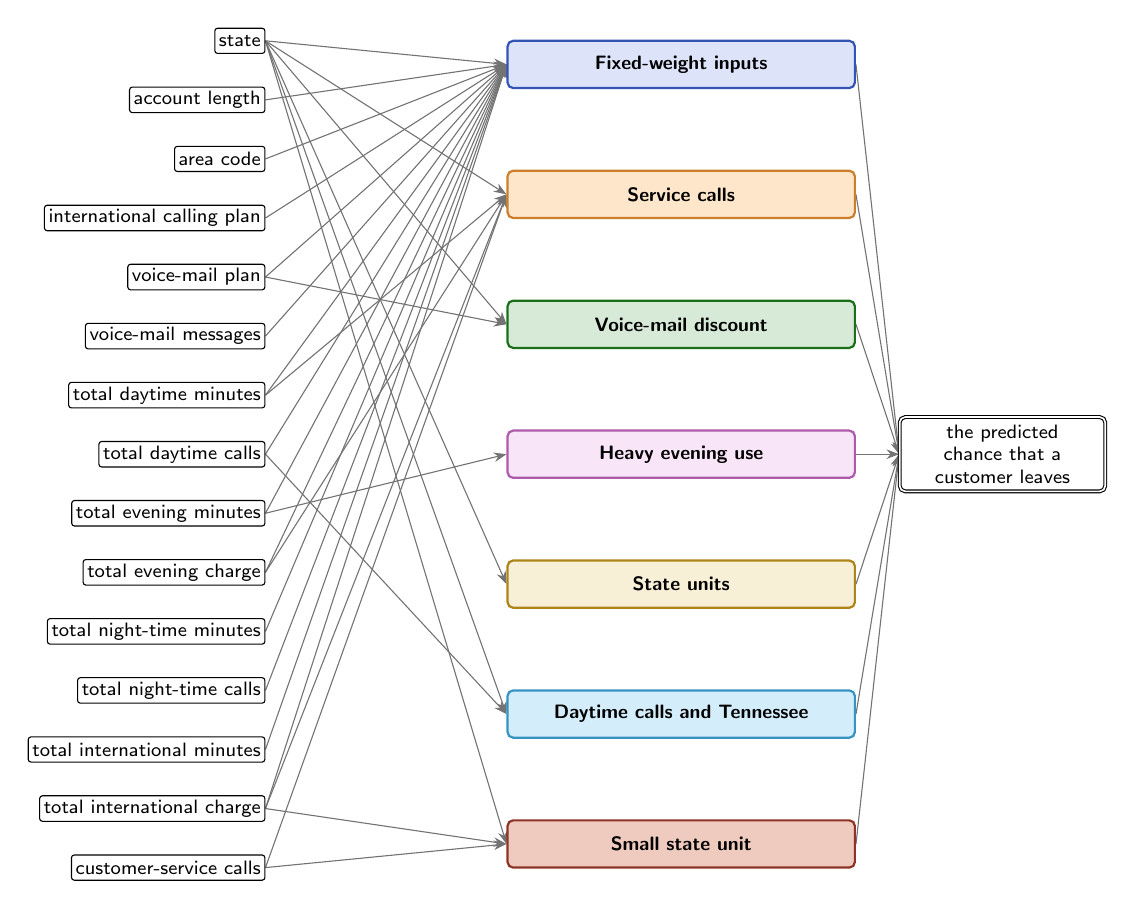
\begin{tikzpicture}[
  font=\sffamily\scriptsize, >={Stealth[length=1.6mm]},
  inp/.style={draw, rounded corners=1pt, fill=white, inner sep=1.5pt, minimum height=3.2mm, anchor=east},
  abox/.style={draw, thick, rounded corners=2pt, align=center, inner sep=3pt, minimum height=6mm, text width=42mm},
  outp/.style={draw, double, rounded corners=2pt, fill=white, align=center, inner sep=3pt, text width=24mm},
  agg/.style={draw=black!55},
]
\node[inp] (i0) at (0,5.25) {state};
\node[inp] (i1) at (0,4.5) {account length};
\node[inp] (i2) at (0,3.75) {area code};
\node[inp] (i3) at (0,3.0) {international calling plan};
\node[inp] (i4) at (0,2.25) {voice-mail plan};
\node[inp] (i5) at (0,1.5) {voice-mail messages};
\node[inp] (i6) at (0,0.75) {total daytime minutes};
\node[inp] (i7) at (0,-0.0) {total daytime calls};
\node[inp] (i8) at (0,-0.75) {total evening minutes};
\node[inp] (i9) at (0,-1.5) {total evening charge};
\node[inp] (i10) at (0,-2.25) {total night-time minutes};
\node[inp] (i11) at (0,-3.0) {total night-time calls};
\node[inp] (i12) at (0,-3.75) {total international minutes};
\node[inp] (i13) at (0,-4.5) {total international charge};
\node[inp] (i14) at (0,-5.25) {customer-service calls};
\node[abox, fill=RoyalBlue!18, draw=RoyalBlue!80!black] (b0) at (5.28,4.95) {\textbf{Fixed-weight inputs}};
\node[abox, fill=BurntOrange!18, draw=BurntOrange!80!black] (b1) at (5.28,3.3) {\textbf{Service calls}};
\node[abox, fill=ForestGreen!18, draw=ForestGreen!80!black] (b2) at (5.28,1.65) {\textbf{Voice-mail discount}};
\node[abox, fill=Orchid!18, draw=Orchid!80!black] (b3) at (5.28,0.0) {\textbf{Heavy evening use}};
\node[abox, fill=Goldenrod!18, draw=Goldenrod!80!black] (b4) at (5.28,-1.65) {\textbf{State units}};
\node[abox, fill=Cerulean!18, draw=Cerulean!80!black] (b5) at (5.28,-3.3) {\textbf{Daytime calls and Tennessee}};
\node[abox, fill=Mahogany!18, draw=Mahogany!80!black] (b6) at (5.28,-4.95) {\textbf{Small state unit}};
\node[outp] (out) at (9.36,0) {the predicted chance that a customer leaves};
\begin{scope}[on background layer]
\draw[->, agg, thin] (i0.east) -- (b0.west);
\draw[->, agg, thin] (i1.east) -- (b0.west);
\draw[->, agg, thin] (i2.east) -- (b0.west);
\draw[->, agg, thin] (i3.east) -- (b0.west);
\draw[->, agg, thin] (i4.east) -- (b0.west);
\draw[->, agg, thin] (i5.east) -- (b0.west);
\draw[->, agg, thin] (i6.east) -- (b0.west);
\draw[->, agg, thin] (i7.east) -- (b0.west);
\draw[->, agg, thin] (i8.east) -- (b0.west);
\draw[->, agg, thin] (i9.east) -- (b0.west);
\draw[->, agg, thin] (i10.east) -- (b0.west);
\draw[->, agg, thin] (i11.east) -- (b0.west);
\draw[->, agg, thin] (i12.east) -- (b0.west);
\draw[->, agg, thin] (i13.east) -- (b0.west);
\draw[->, agg] (b0.east) -- (out.west);
\draw[->, agg, thin] (i0.east) -- (b1.west);
\draw[->, agg, thin] (i6.east) -- (b1.west);
\draw[->, agg, thin] (i9.east) -- (b1.west);
\draw[->, agg, thin] (i13.east) -- (b1.west);
\draw[->, agg, thin] (i14.east) -- (b1.west);
\draw[->, agg] (b1.east) -- (out.west);
\draw[->, agg, thin] (i0.east) -- (b2.west);
\draw[->, agg, thin] (i4.east) -- (b2.west);
\draw[->, agg] (b2.east) -- (out.west);
\draw[->, agg, thin] (i8.east) -- (b3.west);
\draw[->, agg] (b3.east) -- (out.west);
\draw[->, agg, thin] (i0.east) -- (b4.west);
\draw[->, agg] (b4.east) -- (out.west);
\draw[->, agg, thin] (i0.east) -- (b5.west);
\draw[->, agg, thin] (i7.east) -- (b5.west);
\draw[->, agg] (b5.east) -- (out.west);
\draw[->, agg, thin] (i0.east) -- (b6.west);
\draw[->, agg, thin] (i13.east) -- (b6.west);
\draw[->, agg, thin] (i14.east) -- (b6.west);
\draw[->, agg] (b6.east) -- (out.west);
\end{scope}
\end{tikzpicture}}}%
\caption{The model at the level of the summary: one box per part.}
\label{fig:churn100s2c1:summary}
\end{figure}
\paragraph{Fixed-weight inputs.} This part adds up most inputs with fixed weights, and daytime minutes count most: they raise a typical customer's chance of leaving steadily, from under 1\% at 112 to about 13\% at 249 minutes.\,{\scriptsize\textcolor{NavyBlue}{[C057]}} An international plan takes the chance from about 1\% to about 13\%, a voice-mail plan lowers it to under 1\%, and more voice-mail messages raise it steadily, from about 1\% at 0 to about 5\% at 32 messages.\,{\scriptsize\textcolor{NavyBlue}{[C058, C067, C059]}} A higher international charge, more evening minutes, a higher evening charge and more night-time minutes also raise it steadily, each by one to two points.\,{\scriptsize\textcolor{NavyBlue}{[C062, C063, C064, C070]}} Through it, the state moves the chance from about 1\% in West Virginia to about 4\% in California and in Washington, and to under 1\% in Hawaii, Vermont and Colorado (41 to 80 training customers per state).\,{\scriptsize\textcolor{NavyBlue}{[C060, C061, C066, C068, C071]}}
\paragraph{Service calls.} This part adds up two parts: customer-service calls combined with low daytime use, and a rise from 4 calls upwards.\,{\scriptsize\textcolor{NavyBlue}{[C111]}} Through it, daytime minutes lower the chance only while they stay below about 170 minutes (between 147 and 216 minutes for different customers), in an uneven way: for a typical customer, from about 38\% at 91 minutes to about 1\% at 352 minutes.\,{\scriptsize\textcolor{NavyBlue}{[C107]}} With an evening charge above 17.12 US dollars, the chance is lowest at about 154 minutes of daytime use and higher either side: from about 1\% at 112 minutes to about 17\% at 249 minutes, against about 2\% to about 10\% at or below that charge.\,{\scriptsize\textcolor{NavyBlue}{[C103]}} Customer-service calls add to it from 4 calls upwards, in an uneven way: for a typical such customer, from about 3\% at 0 calls to about 11\% at 4 calls.\,{\scriptsize\textcolor{NavyBlue}{[C108]}}
\paragraph{Voice-mail discount.} This part reads the voice-mail plan and a few states: through it, a voice-mail plan lowers a typical customer's chance by less than a point, and customers in states other than Alabama, North Carolina and West Virginia get about 2\% instead of about 1\%.\,{\scriptsize\textcolor{NavyBlue}{[C125, C126]}}
\paragraph{Heavy evening use.} Through this part, evening minutes add nothing until about 239 minutes, then lower the chance steadily; it acts on 885 of 4000 training customers, 165 of whom left, and for the typical customer it acts on, the chance is about 5\% without it and about 4\% with it.\,{\scriptsize\textcolor{NavyBlue}{[C135, C136]}}
\paragraph{State units.} This part reads only the state and moves the chance by less than half a point: up in Arizona and Ohio, down in Nevada.\,{\scriptsize\textcolor{NavyBlue}{[C138, C139, C140]}}
\paragraph{Daytime calls and Tennessee.} This part reads the state and daytime calls: being in Tennessee raises a typical customer's chance from about 1\% to about 2\%, and daytime calls barely change it.\,{\scriptsize\textcolor{NavyBlue}{[C144, C145]}}
\paragraph{Small state unit.} This small part moves the chance by less than a tenth of a point, up in Arkansas and Utah.\,{\scriptsize\textcolor{NavyBlue}{[C150, C153]}}
\paragraph{The whole network.} Figure~\ref{fig:churn100s2c1:overview} (next page, landscape) draws every unit and connection of the explained model, nested by part: shaded clusters are the parts of the model and darker boxes the parts inside them; circles are hidden units (h1, h2, \ldots); each cluster's rectangle is its output, and a dashed `sum' stands for an addition the next unit does (drawn, not a unit of the model); the hexagon is the model's output. An input used by several parts is drawn under each of them (same label, dotted outline, the first copy marked with the number of copies): it is the same input, repeated for readability. Not used by the model (input columns with no connection): state: 20 of 51 levels, total daytime charge, total evening calls, total night-time charge, total international calls.
\begin{landscape}
\begin{figure}[p]\centering
\resizebox{\linewidth}{!}{%
\definecolor{netup}{HTML}{D95F02}\definecolor{netdown}{HTML}{1B9E77}\definecolor{netmixed}{HTML}{7F7F7F}%
\begin{tikzpicture}[
  font=\sffamily\scriptsize, >={Stealth[length=1.4mm]},
  inp/.style={draw, circle, fill=white, minimum size=3.2mm, inner sep=0pt},
  hid/.style={draw, circle, fill=white, minimum size=5.2mm, inner sep=0.5pt, font=\sffamily\tiny},
  exitbox/.style={draw, thick, rectangle, fill=white, align=center, text width=17mm, minimum height=5mm, inner sep=1.5pt, font=\sffamily\tiny},
  sumbox/.style={draw, thick, dashed, rectangle, fill=white, align=center, text width=17mm, minimum height=5mm, inner sep=1.5pt, font=\sffamily\tiny},
  outp/.style={draw, thick, regular polygon, regular polygon sides=6, fill=white, minimum size=10mm, inner sep=0pt, font=\sffamily\tiny, align=center},
  stub/.style={draw, dashed, rounded corners=2pt, fill=white, align=center, inner sep=2pt, font=\sffamily\tiny, text width=15mm},
  inlab/.style={font=\sffamily\tiny, align=center, text width=15mm, inner sep=1pt, fill=white, fill opacity=0.8, text opacity=1},
  wpos/.style={draw=NavyBlue}, wneg/.style={draw=BrickRed}, wagg/.style={draw=black!45, line width=1.2pt},
  wmix/.style={draw=Plum},
]
\node[outp] (n0) at (27.65,8.85) {churn};
\node[hid] (n10249) at (35.07,1.9) {h14};
\node[hid] (n1133) at (26.34,3.25) {h5};
\node[exitbox] (n11427) at (45.66,1.9) {Daytime calls and Tennessee $\uparrow$};
\node[hid] (n11951) at (36.57,1.9) {h16};
\node[hid] (n1264) at (14.74,5.95) {h6};
\node[hid] (n12926) at (13.99,1.9) {h17};
\node[hid] (n13827) at (38.07,4.6) {h18};
\node[hid] (n14942) at (38.07,1.9) {h19};
\node[hid] (n161) at (51.85,1.9) {h1};
\node[hid] (n17032) at (18.57,1.9) {h20};
\node[exitbox] (n252) at (52.6,4.6) {Small state unit $\uparrow$};
\node[hid] (n2627xa) at (52.6,3.25) {h21};
\node[hid] (n2627xb) at (13.99,3.25) {h22};
\node[hid] (n2796) at (15.49,3.25) {h7};
\node[hid] (n3861) at (39.57,1.9) {h8};
\node[hid] (n4051) at (26.34,4.6) {h9};
\node[exitbox] (n476) at (31.48,1.9) {Heavy evening use $\downarrow$};
\node[hid] (n5577) at (26.34,1.9) {h10};
\node[hid] (n6730) at (38.07,3.25) {h11};
\node[hid] (n7208) at (18.57,3.25) {h12};
\node[hid] (n807) at (14.74,4.6) {h4};
\node[hid] (n8896) at (41.07,1.9) {h13};
\node[hid] (n9555xa) at (53.35,1.9) {h23};
\node[hid] (n9555xb) at (15.49,1.9) {h24};
\node[exitbox] (nidentityxlin) at (5.85,1.9) {Fixed-weight inputs $\uparrow$};
\node[exitbox] (nidentityxsvc) at (21.9,7.3) {Service calls $\uparrow$};
\node[sumbox] (ncsumxxannx95) at (26.34,5.95) {sum: Voice-mail discount $\downarrow$};
\node[sumbox] (ncsumxxannx96) at (38.07,5.95) {sum: State units $\updownarrow$};
\node[inp, densely dotted, thick, draw=netmixed, very thick] (ngrpxxstatexxannx92) at (50.8,0.0) {};
\path (ngrpxxstatexxannx92.south) node[inlab, anchor=north] (labngrpxxstatexxannx92) {state (31 of 51 used) ($\times$6) $\updownarrow$};
\node[inp, densely dotted, thick, draw=netmixed, very thick] (ngrpxxstatexxannx95) at (27.24,0.0) {};
\path (ngrpxxstatexxannx95.south) node[inlab, anchor=north] (labngrpxxstatexxannx95) {state (31 of 51 used) $\updownarrow$};
\node[inp, densely dotted, thick, draw=netmixed, very thick] (ngrpxxstatexxannx96) at (38.07,0.0) {};
\path (ngrpxxstatexxannx96.south) node[inlab, anchor=north] (labngrpxxstatexxannx96) {state (31 of 51 used) $\updownarrow$};
\node[inp, densely dotted, thick, draw=netmixed, very thick] (ngrpxxstatexxannx97) at (44.76,0.0) {};
\path (ngrpxxstatexxannx97.south) node[inlab, anchor=north] (labngrpxxstatexxannx97) {state (31 of 51 used) $\updownarrow$};
\node[inp, densely dotted, thick, draw=netup, very thick] (ninxxnumberxcustomerxservicexcallsxxannx101) at (18.07,0.0) {};
\path (ninxxnumberxcustomerxservicexcallsxxannx101.south) node[inlab, anchor=north] (labninxxnumberxcustomerxservicexcallsxxannx101) {customer-service calls ($\times$2) $\uparrow$};
\node[inp, densely dotted, thick, draw=netdown, very thick] (ninxxtotalxintlxchargexxannx92) at (52.6,0.0) {};
\path (ninxxtotalxintlxchargexxannx92.south) node[inlab, anchor=north] (labninxxtotalxintlxchargexxannx92) {total international charge ($\times$3) $\downarrow$};
\node[inp, densely dotted, thick, draw=netdown, very thick] (ninxxtotalxintlxchargexxannx101) at (16.27,0.0) {};
\path (ninxxtotalxintlxchargexxannx101.south) node[inlab, anchor=north] (labninxxtotalxintlxchargexxannx101) {total international charge $\downarrow$};
\node[inp, densely dotted, thick, draw=netdown, very thick] (ninxxtotalxevexchargexxannx101) at (19.87,0.0) {};
\path (ninxxtotalxevexchargexxannx101.south) node[inlab, anchor=north] (labninxxtotalxevexchargexxannx101) {total evening charge ($\times$2) $\downarrow$};
\node[inp, densely dotted, thick, draw=netdown, very thick] (ninxxtotalxevexminutesxxannx94) at (31.48,0.0) {};
\path (ninxxtotalxevexminutesxxannx94.south) node[inlab, anchor=north] (labninxxtotalxevexminutesxxannx94) {total evening minutes ($\times$2) $\downarrow$};
\node[inp, densely dotted, thick, draw=netdown, very thick] (ninxxtotalxdayxcallsxxannx97) at (46.56,0.0) {};
\path (ninxxtotalxdayxcallsxxannx97.south) node[inlab, anchor=north] (labninxxtotalxdayxcallsxxannx97) {total daytime calls ($\times$2) $\downarrow$};
\node[inp, densely dotted, thick, draw=netdown, very thick] (ninxxtotalxdayxminutesxxannx101) at (14.47,0.0) {};
\path (ninxxtotalxdayxminutesxxannx101.south) node[inlab, anchor=north] (labninxxtotalxdayxminutesxxannx101) {total daytime minutes ($\times$2) $\downarrow$};
\node[inp, densely dotted, thick, draw=netdown, very thick] (ninxxvoicexmailxplanxxannx95) at (25.44,0.0) {};
\path (ninxxvoicexmailxplanxxannx95.south) node[inlab, anchor=north] (labninxxvoicexmailxplanxxannx95) {a voice-mail plan ($\times$2) $\downarrow$};
\node[inp, densely dotted, thick, draw=netmixed, very thick] (ngrpxxstatexxannx101) at (21.67,0.0) {};
\path (ngrpxxstatexxannx101.south) node[inlab, anchor=north] (labngrpxxstatexxannx101) {state (31 of 51 used) $\updownarrow$};
\node[inp, densely dotted, thick, draw=netdown, very thick] (ninxxnumberxcustomerxservicexcallsxxannx92) at (54.4,0.0) {};
\path (ninxxnumberxcustomerxservicexcallsxxannx92.south) node[inlab, anchor=north] (labninxxnumberxcustomerxservicexcallsxxannx92) {customer-service calls $\downarrow$};
\node[inp, densely dotted, thick, draw=netmixed, very thick] (ngrpxxstatexxannx99) at (4.5,0.0) {};
\path (ngrpxxstatexxannx99.south) node[inlab, anchor=north] (labngrpxxstatexxannx99) {state (31 of 51 used) $\updownarrow$};
\node[inp, draw=netup, very thick] (ninxxaccountxlengthxxannx99) at (0.9,-2.1) {};
\path (ninxxaccountxlengthxxannx99.south) node[inlab, anchor=north] (labninxxaccountxlengthxxannx99) {account length $\uparrow$};
\node[inp, draw=netdown, very thick] (ninxxareaxcodex408xxannx99) at (2.7,0.0) {};
\path (ninxxareaxcodex408xxannx99.south) node[inlab, anchor=north] (labninxxareaxcodex408xxannx99) {area code 408 $\downarrow$};
\node[inp, draw=netup, very thick] (ninxxareaxcodex415xxannx99) at (2.7,-2.1) {};
\path (ninxxareaxcodex415xxannx99.south) node[inlab, anchor=north] (labninxxareaxcodex415xxannx99) {area code 415 $\uparrow$};
\node[inp, draw=netdown, very thick] (ninxxareaxcodex510xxannx99) at (3.6,-1.05) {};
\path (ninxxareaxcodex510xxannx99.south) node[inlab, anchor=north] (labninxxareaxcodex510xxannx99) {area code 510 $\downarrow$};
\node[inp, draw=netup, very thick] (ninxxinternationalxplanxxannx99) at (1.8,-1.05) {};
\path (ninxxinternationalxplanxxannx99.south) node[inlab, anchor=north] (labninxxinternationalxplanxxannx99) {an international plan $\uparrow$};
\node[inp, draw=netup, very thick] (ninxxnumberxvmailxmessagesxxannx99) at (10.8,-1.05) {};
\path (ninxxnumberxvmailxmessagesxxannx99.south) node[inlab, anchor=north] (labninxxnumberxvmailxmessagesxxannx99) {voice-mail messages $\uparrow$};
\node[inp, draw=netup, very thick] (ninxxtotalxnightxminutesxxannx99) at (9.9,0.0) {};
\path (ninxxtotalxnightxminutesxxannx99.south) node[inlab, anchor=north] (labninxxtotalxnightxminutesxxannx99) {total night-time minutes $\uparrow$};
\node[inp, draw=netdown, very thick] (ninxxtotalxnightxcallsxxannx99) at (9.0,-1.05) {};
\path (ninxxtotalxnightxcallsxxannx99.south) node[inlab, anchor=north] (labninxxtotalxnightxcallsxxannx99) {total night-time calls $\downarrow$};
\node[inp, draw=netdown, very thick] (ninxxtotalxintlxminutesxxannx99) at (8.1,0.0) {};
\path (ninxxtotalxintlxminutesxxannx99.south) node[inlab, anchor=north] (labninxxtotalxintlxminutesxxannx99) {total international minutes $\downarrow$};
\node[inp, densely dotted, thick, draw=netup, very thick] (ninxxtotalxintlxchargexxannx99) at (7.2,-1.05) {};
\path (ninxxtotalxintlxchargexxannx99.south) node[inlab, anchor=north] (labninxxtotalxintlxchargexxannx99) {total international charge $\uparrow$};
\node[inp, densely dotted, thick, draw=netup, very thick] (ninxxtotalxevexchargexxannx99) at (6.3,0.0) {};
\path (ninxxtotalxevexchargexxannx99.south) node[inlab, anchor=north] (labninxxtotalxevexchargexxannx99) {total evening charge $\uparrow$};
\node[inp, densely dotted, thick, draw=netup, very thick] (ninxxtotalxevexminutesxxannx99) at (6.3,-2.1) {};
\path (ninxxtotalxevexminutesxxannx99.south) node[inlab, anchor=north] (labninxxtotalxevexminutesxxannx99) {total evening minutes $\uparrow$};
\node[inp, densely dotted, thick, draw=netup, very thick] (ninxxtotalxdayxcallsxxannx99) at (4.5,-2.1) {};
\path (ninxxtotalxdayxcallsxxannx99.south) node[inlab, anchor=north] (labninxxtotalxdayxcallsxxannx99) {total daytime calls $\uparrow$};
\node[inp, densely dotted, thick, draw=netup, very thick] (ninxxtotalxdayxminutesxxannx99) at (5.4,-1.05) {};
\path (ninxxtotalxdayxminutesxxannx99.south) node[inlab, anchor=north] (labninxxtotalxdayxminutesxxannx99) {total daytime minutes $\uparrow$};
\node[inp, densely dotted, thick, draw=netdown, very thick] (ninxxvoicexmailxplanxxannx99) at (0.9,0.0) {};
\path (ninxxvoicexmailxplanxxannx99.south) node[inlab, anchor=north] (labninxxvoicexmailxplanxxannx99) {a voice-mail plan $\downarrow$};
\node[font=\sffamily\tiny\bfseries, text=ForestGreen!60!black, inner sep=1pt] (subt0) at (14.74,6.45) {Calls with low usage};
\node[font=\sffamily\tiny\bfseries, text=ForestGreen!60!black, inner sep=1pt] (subt1) at (18.57,3.75) {Many service calls};
\begin{scope}[on background layer]
\node[fit=(nidentityxlin) , inner sep=8pt, rounded corners=5pt, fill=BurntOrange!10, draw=BurntOrange!45] (clu1) {};
\node[fit=(n1264) (n12926) (n17032) (n2627xb) (n2796) (n7208) (n807) (n9555xb) (nidentityxsvc) (subt0) (subt1), inner sep=8pt, rounded corners=5pt, fill=ForestGreen!10, draw=ForestGreen!45] (clu2) {};
\node[fit=(n1133) (n4051) (n5577) (ncsumxxannx95) , inner sep=8pt, rounded corners=5pt, fill=Orchid!10, draw=Orchid!45] (clu3) {};
\node[fit=(n476) , inner sep=8pt, rounded corners=5pt, fill=Goldenrod!10, draw=Goldenrod!45] (clu4) {};
\node[fit=(n10249) (n11951) (n13827) (n14942) (n3861) (n6730) (n8896) (ncsumxxannx96) , inner sep=8pt, rounded corners=5pt, fill=Cerulean!10, draw=Cerulean!45] (clu5) {};
\node[fit=(n11427) , inner sep=8pt, rounded corners=5pt, fill=Mahogany!10, draw=Mahogany!45] (clu6) {};
\node[fit=(n161) (n252) (n2627xa) (n9555xa) , inner sep=8pt, rounded corners=5pt, fill=OliveGreen!10, draw=OliveGreen!45] (clu7) {};
\node[fit=(n1264) (n12926) (n2627xb) (n2796) (n807) (n9555xb) (subt0), inner sep=4pt, rounded corners=3pt, fill=ForestGreen!26, draw=ForestGreen!70] {};
\node[fit=(n17032) (n7208) (subt1), inner sep=4pt, rounded corners=3pt, fill=ForestGreen!26, draw=ForestGreen!70] {};
\draw[->, wpos, line width=0.26pt] (n252) -- (n0);
\draw[->, wneg, line width=0.44pt] (n476) -- (n0);
\draw[->, wneg, line width=0.58pt] (n1133) -- (ncsumxxannx95);
\draw[->, wneg, line width=0.30pt] (n3861) -- (ncsumxxannx96);
\draw[->, wneg, line width=0.60pt] (n4051) -- (ncsumxxannx95);
\draw[->, wpos, line width=0.26pt] (n8896) -- (ncsumxxannx96);
\draw[->, wpos, line width=0.26pt] (n10249) -- (ncsumxxannx96);
\draw[->, wpos, line width=0.27pt] (n11427) -- (n0);
\draw[->, wpos, line width=0.40pt] (n13827) -- (ncsumxxannx96);
\draw[->, wpos, line width=0.26pt] (n14942) -- (ncsumxxannx96);
\draw[->, wpos, line width=0.53pt] (n161) -- (n252);
\draw[->, wpos, line width=0.47pt] (n2796) -- (n807);
\draw[->, wpos, line width=0.38pt] (n807) -- (n1264);
\draw[->, wpos, line width=0.65pt] (n1133) -- (n4051);
\draw[->, wpos, line width=0.30pt] (n5577) -- (n1133);
\draw[->, wneg, line width=0.25pt] (n11951) -- (n6730);
\draw[->, wpos, line width=0.37pt] (n12926) -- (n2796);
\draw[->, wpos, line width=0.44pt] (n17032) -- (n7208);
\draw[->, wpos, line width=0.60pt] (n6730) -- (n13827);
\draw[->, wneg, line width=0.38pt] (n2627xa) -- (n252);
\draw[->, wpos, line width=0.49pt] (n2627xb) -- (n807);
\draw[->, wpos, line width=0.36pt] (n9555xa) -- (n2627xa);
\draw[->, wpos, line width=0.36pt] (n9555xb) -- (n2627xb);
\draw[->, wpos, line width=0.60pt] (ninxxnumberxcustomerxservicexcallsxxannx101) -- (n17032);
\draw[->, wneg, line width=0.55pt] (ninxxtotalxintlxchargexxannx92) -- (n252);
\draw[->, wneg, line width=0.36pt] (ninxxtotalxintlxchargexxannx101) -- (n1264);
\draw[->, wneg, line width=0.60pt] (ninxxtotalxevexchargexxannx101) -- (n2796);
\draw[->, wpos, line width=0.63pt] (ninxxtotalxevexminutesxxannx94) -- (n476);
\draw[->, wneg, line width=0.29pt] (ninxxtotalxdayxcallsxxannx97) -- (n11427);
\draw[->, wneg, line width=0.74pt] (ninxxtotalxdayxminutesxxannx101) -- (n807);
\draw[->, wpos, line width=0.60pt] (ninxxvoicexmailxplanxxannx95) -- (n5577);
\draw[->, wpos, line width=0.26pt] (ninxxnumberxcustomerxservicexcallsxxannx101) -- (n807);
\draw[->, wpos, line width=0.38pt] (ninxxnumberxcustomerxservicexcallsxxannx101) -- (n2796);
\draw[->, wpos, line width=0.60pt] (ninxxnumberxcustomerxservicexcallsxxannx101) -- (n12926);
\draw[->, wpos, line width=0.35pt] (ninxxnumberxcustomerxservicexcallsxxannx101) -- (n2627xb);
\draw[->, wpos, line width=0.55pt] (ninxxnumberxcustomerxservicexcallsxxannx101) -- (n9555xb);
\draw[->, wpos, line width=0.35pt] (ninxxnumberxcustomerxservicexcallsxxannx92) -- (n2627xa);
\draw[->, wpos, line width=0.55pt] (ninxxnumberxcustomerxservicexcallsxxannx92) -- (n9555xa);
\draw[->, wpos, line width=0.30pt] (ninxxaccountxlengthxxannx99) -- (nidentityxlin);
\draw[->, wneg, line width=0.26pt] (ninxxareaxcodex408xxannx99) -- (nidentityxlin);
\draw[->, wpos, line width=0.27pt] (ninxxareaxcodex415xxannx99) -- (nidentityxlin);
\draw[->, wneg, line width=0.26pt] (ninxxareaxcodex510xxannx99) -- (nidentityxlin);
\draw[->, wpos, line width=0.51pt] (ninxxinternationalxplanxxannx99) -- (nidentityxlin);
\draw[->, wpos, line width=0.47pt] (ninxxnumberxvmailxmessagesxxannx99) -- (nidentityxlin);
\draw[->, wpos, line width=0.36pt] (ninxxtotalxnightxminutesxxannx99) -- (nidentityxlin);
\draw[->, wneg, line width=0.25pt] (ninxxtotalxnightxcallsxxannx99) -- (nidentityxlin);
\draw[->, wneg, line width=0.26pt] (ninxxtotalxintlxminutesxxannx99) -- (nidentityxlin);
\draw[->, wpos, line width=0.50pt] (ninxxtotalxintlxchargexxannx99) -- (nidentityxlin);
\draw[->, wpos, line width=0.41pt] (ninxxtotalxevexchargexxannx99) -- (nidentityxlin);
\draw[->, wpos, line width=0.43pt] (ninxxtotalxevexminutesxxannx99) -- (nidentityxlin);
\draw[->, wpos, line width=0.29pt] (ninxxtotalxdayxcallsxxannx99) -- (nidentityxlin);
\draw[->, wpos, line width=0.96pt] (ninxxtotalxdayxminutesxxannx99) -- (nidentityxlin);
\draw[->, wneg, line width=0.56pt] (ninxxvoicexmailxplanxxannx99) -- (nidentityxlin);
\draw[->, wpos, line width=0.60pt] (nidentityxlin) -- (n0);
\draw[->, wpos, line width=0.81pt] (n807) -- (nidentityxsvc);
\draw[->, wpos, line width=0.88pt] (n1264) -- (nidentityxsvc);
\draw[->, wpos, line width=0.77pt] (n7208) -- (nidentityxsvc);
\draw[->, wpos, line width=0.60pt] (nidentityxsvc) -- (n0);
\draw[->, wagg] (ncsumxxannx95) -- (n0);
\draw[->, wagg] (ncsumxxannx96) -- (n0);
\draw[->, wneg, line width=0.25pt] (ngrpxxstatexxannx92) -- node[pos=0.8, sloped, above, font=\sffamily\tiny, inner sep=1pt, fill=white, fill opacity=0.8, text opacity=1] {-0.01} (n161);
\draw[->, wpos, line width=0.34pt] (ngrpxxstatexxannx95) -- node[pos=0.8, sloped, above, font=\sffamily\tiny, inner sep=1pt, fill=white, fill opacity=0.8, text opacity=1] {+0.26} (n5577);
\draw[->, wpos, line width=0.52pt] (ngrpxxstatexxannx92) -- node[pos=0.8, sloped, above, font=\sffamily\tiny, inner sep=1pt, fill=white, fill opacity=0.8, text opacity=1] {2 edges, +0.44 to +0.76} (n252);
\draw[->, wneg, line width=0.60pt] (ngrpxxstatexxannx96) -- node[pos=0.8, sloped, above, font=\sffamily\tiny, inner sep=1pt, fill=white, fill opacity=0.8, text opacity=1] {-1.00} (n8896);
\draw[->, wmix, line width=0.40pt] (ngrpxxstatexxannx96) -- node[pos=0.8, sloped, above, font=\sffamily\tiny, inner sep=1pt, fill=white, fill opacity=0.8, text opacity=1] {3 edges, -0.42 to +0.00} (n6730);
\draw[->, wpos, line width=0.60pt] (ngrpxxstatexxannx97) -- node[pos=0.8, sloped, above, font=\sffamily\tiny, inner sep=1pt, fill=white, fill opacity=0.8, text opacity=1] {+1.00} (n11427);
\draw[->, wneg, line width=0.52pt] (ngrpxxstatexxannx96) -- node[pos=0.8, sloped, above, font=\sffamily\tiny, inner sep=1pt, fill=white, fill opacity=0.8, text opacity=1] {-0.77} (n3861);
\draw[->, wpos, line width=0.27pt] (ngrpxxstatexxannx95) -- node[pos=0.8, sloped, above, font=\sffamily\tiny, inner sep=1pt, fill=white, fill opacity=0.8, text opacity=1] {+0.06} (n4051);
\draw[->, wneg, line width=0.38pt] (ngrpxxstatexxannx101) -- node[pos=0.8, sloped, above, font=\sffamily\tiny, inner sep=1pt, fill=white, fill opacity=0.8, text opacity=1] {-0.36} (n7208);
\draw[->, wpos, line width=0.30pt] (ngrpxxstatexxannx101) -- node[pos=0.8, sloped, above, font=\sffamily\tiny, inner sep=1pt, fill=white, fill opacity=0.8, text opacity=1] {+0.15} (n2796);
\draw[->, wpos, line width=0.60pt] (ngrpxxstatexxannx96) -- node[pos=0.8, sloped, above, font=\sffamily\tiny, inner sep=1pt, fill=white, fill opacity=0.8, text opacity=1] {+1.00} (n10249);
\draw[->, wpos, line width=0.26pt] (ngrpxxstatexxannx95) -- node[pos=0.8, sloped, above, font=\sffamily\tiny, inner sep=1pt, fill=white, fill opacity=0.8, text opacity=1] {+0.02} (n1133);
\draw[->, wpos, line width=0.60pt] (ngrpxxstatexxannx96) -- node[pos=0.8, sloped, above, font=\sffamily\tiny, inner sep=1pt, fill=white, fill opacity=0.8, text opacity=1] {+1.00} (n11951);
\draw[->, wpos, line width=0.60pt] (ngrpxxstatexxannx96) -- node[pos=0.8, sloped, above, font=\sffamily\tiny, inner sep=1pt, fill=white, fill opacity=0.8, text opacity=1] {+1.00} (n14942);
\draw[->, wmix, line width=0.36pt] (ngrpxxstatexxannx99) -- node[pos=0.8, sloped, above, font=\sffamily\tiny, inner sep=1pt, fill=white, fill opacity=0.8, text opacity=1] {25 edges, -0.30 to +0.15} (nidentityxlin);
\end{scope}
\node[font=\sffamily\scriptsize\bfseries, text=BurntOrange!55!black, anchor=south west, inner sep=1pt, fill=white, fill opacity=0.85, text opacity=1] at (clu1.north west) {Fixed-weight inputs};
\node[font=\sffamily\scriptsize\bfseries, text=ForestGreen!55!black, anchor=south west, inner sep=1pt, fill=white, fill opacity=0.85, text opacity=1] at (clu2.north west) {Service calls};
\node[font=\sffamily\scriptsize\bfseries, text=Orchid!55!black, anchor=south west, inner sep=1pt, fill=white, fill opacity=0.85, text opacity=1] at (clu3.north west) {Voice-mail discount};
\node[font=\sffamily\scriptsize\bfseries, text=Goldenrod!55!black, anchor=south west, inner sep=1pt, fill=white, fill opacity=0.85, text opacity=1] at (clu4.north west) {Heavy evening use};
\node[font=\sffamily\scriptsize\bfseries, text=Cerulean!55!black, anchor=south west, inner sep=1pt, fill=white, fill opacity=0.85, text opacity=1] at (clu5.north west) {State units};
\node[font=\sffamily\scriptsize\bfseries, text=Mahogany!55!black, anchor=south west, inner sep=1pt, fill=white, fill opacity=0.85, text opacity=1] at (clu6.north west) {Daytime calls and Tennessee};
\node[font=\sffamily\scriptsize\bfseries, text=OliveGreen!55!black, anchor=south west, inner sep=1pt, fill=white, fill opacity=0.85, text opacity=1] at (clu7.north west) {Small state unit};
\end{tikzpicture}}%
\caption{Every unit and connection of the explained model, nested by part. Blue: positive weight (raises the score); red: negative weight (lowers it); thicker: larger weight. Orange outline and up arrow: raises the final prediction; teal and down arrow: lowers it; grey and double arrow: depends.}
\label{fig:churn100s2c1:overview}
\end{figure}
\end{landscape}
\paragraph{Worth checking against what is known.} Worth checking: the state moves the chance by several points (for example California and Washington about 6\% and 5\%, Hawaii under 1\%), based on 41 to 122 training customers per state.\,{\scriptsize\textcolor{NavyBlue}{[C003, C004, C016]}} Worth checking: the model treats a voice-mail plan as lowering the chance of leaving but more voice-mail messages as raising it.\,{\scriptsize\textcolor{NavyBlue}{[C012, C005]}} Worth checking: the many-service-calls part is switched off for customers in West Virginia, the state of the typical customer.\,{\scriptsize\textcolor{NavyBlue}{[C130]}} Worth checking: daytime minutes, the evening charge and the international charge raise the chance through the fixed-weight inputs but lower it through calls with low usage.\,{\scriptsize\textcolor{NavyBlue}{[C057, C112, C064, C115, C062, C114]}}
\subsection{The model, read from the top down}
\noindent{\small Each part of the explanation in turn, from the whole model down to the smallest parts: what it does for the prediction (hypothesis), what was checked (evidence), a diagram one level down, and where to read on. The technical record of each part is in ``Technical detail'' at the end.\par}
\subsubsection{The whole model}\label{rd:ann102}
\noindent{\small Figure~\ref{fig:churn100s2c1:parts-ann102} shows what feeds this part; Figure~\ref{fig:churn100s2c1:units-ann102} its units and every connection into them (dashed boxes: connections from or to other parts, drawn in their own sections).\par}
\begin{figure}[H]\centering
\resizebox{!}{\ifdim\height>0.5\textheight 0.5\textheight\else\height\fi}{%
\resizebox{\ifdim\width>\linewidth\linewidth\else\width\fi}{!}{%
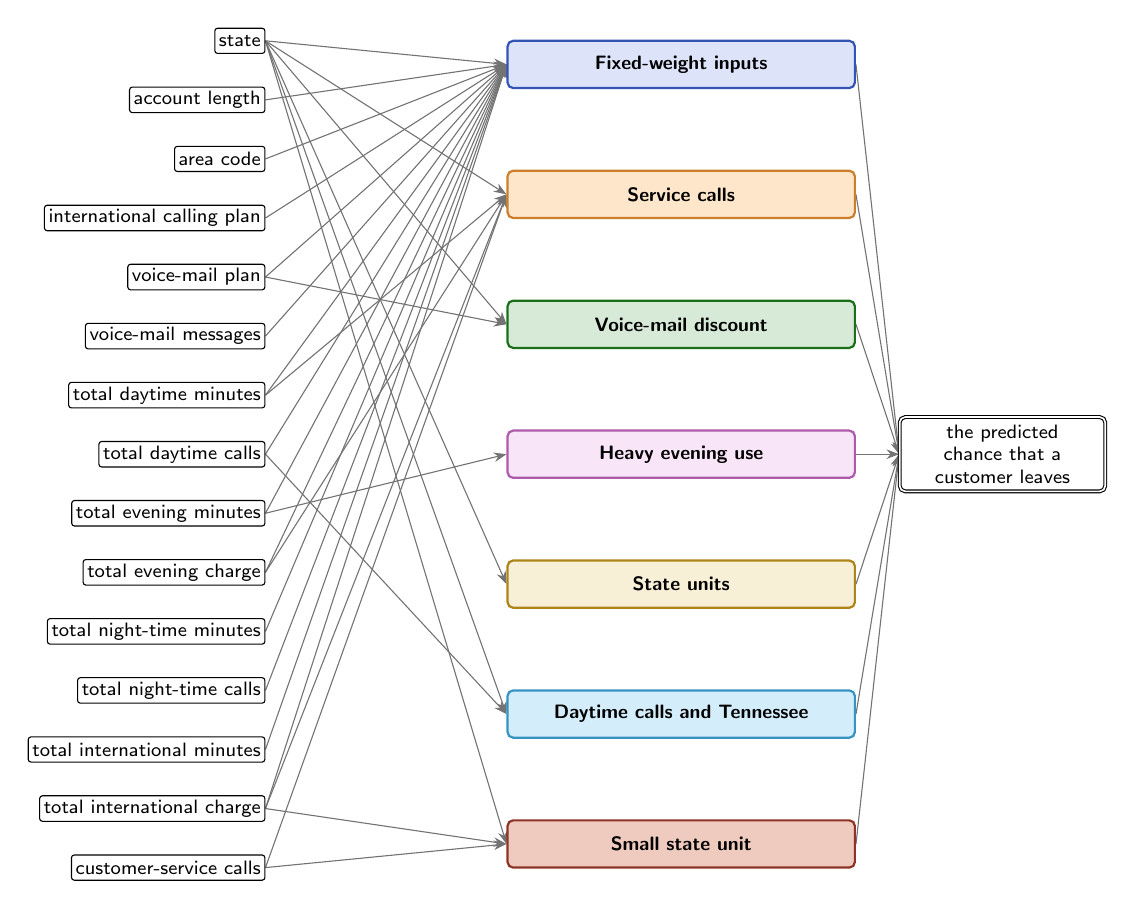
\begin{tikzpicture}[
  font=\sffamily\scriptsize, >={Stealth[length=1.6mm]},
  inp/.style={draw, rounded corners=1pt, fill=white, inner sep=1.5pt, minimum height=3.2mm, anchor=east},
  abox/.style={draw, thick, rounded corners=2pt, align=center, inner sep=3pt, minimum height=6mm, text width=42mm},
  outp/.style={draw, double, rounded corners=2pt, fill=white, align=center, inner sep=3pt, text width=24mm},
  agg/.style={draw=black!55},
]
\node[inp] (i0) at (0,5.25) {state};
\node[inp] (i1) at (0,4.5) {account length};
\node[inp] (i2) at (0,3.75) {area code};
\node[inp] (i3) at (0,3.0) {international calling plan};
\node[inp] (i4) at (0,2.25) {voice-mail plan};
\node[inp] (i5) at (0,1.5) {voice-mail messages};
\node[inp] (i6) at (0,0.75) {total daytime minutes};
\node[inp] (i7) at (0,-0.0) {total daytime calls};
\node[inp] (i8) at (0,-0.75) {total evening minutes};
\node[inp] (i9) at (0,-1.5) {total evening charge};
\node[inp] (i10) at (0,-2.25) {total night-time minutes};
\node[inp] (i11) at (0,-3.0) {total night-time calls};
\node[inp] (i12) at (0,-3.75) {total international minutes};
\node[inp] (i13) at (0,-4.5) {total international charge};
\node[inp] (i14) at (0,-5.25) {customer-service calls};
\node[abox, fill=RoyalBlue!18, draw=RoyalBlue!80!black] (b0) at (5.28,4.95) {\textbf{Fixed-weight inputs}};
\node[abox, fill=BurntOrange!18, draw=BurntOrange!80!black] (b1) at (5.28,3.3) {\textbf{Service calls}};
\node[abox, fill=ForestGreen!18, draw=ForestGreen!80!black] (b2) at (5.28,1.65) {\textbf{Voice-mail discount}};
\node[abox, fill=Orchid!18, draw=Orchid!80!black] (b3) at (5.28,0.0) {\textbf{Heavy evening use}};
\node[abox, fill=Goldenrod!18, draw=Goldenrod!80!black] (b4) at (5.28,-1.65) {\textbf{State units}};
\node[abox, fill=Cerulean!18, draw=Cerulean!80!black] (b5) at (5.28,-3.3) {\textbf{Daytime calls and Tennessee}};
\node[abox, fill=Mahogany!18, draw=Mahogany!80!black] (b6) at (5.28,-4.95) {\textbf{Small state unit}};
\node[outp] (out) at (9.36,0) {the predicted chance that a customer leaves};
\begin{scope}[on background layer]
\draw[->, agg, thin] (i0.east) -- (b0.west);
\draw[->, agg, thin] (i1.east) -- (b0.west);
\draw[->, agg, thin] (i2.east) -- (b0.west);
\draw[->, agg, thin] (i3.east) -- (b0.west);
\draw[->, agg, thin] (i4.east) -- (b0.west);
\draw[->, agg, thin] (i5.east) -- (b0.west);
\draw[->, agg, thin] (i6.east) -- (b0.west);
\draw[->, agg, thin] (i7.east) -- (b0.west);
\draw[->, agg, thin] (i8.east) -- (b0.west);
\draw[->, agg, thin] (i9.east) -- (b0.west);
\draw[->, agg, thin] (i10.east) -- (b0.west);
\draw[->, agg, thin] (i11.east) -- (b0.west);
\draw[->, agg, thin] (i12.east) -- (b0.west);
\draw[->, agg, thin] (i13.east) -- (b0.west);
\draw[->, agg] (b0.east) -- (out.west);
\draw[->, agg, thin] (i0.east) -- (b1.west);
\draw[->, agg, thin] (i6.east) -- (b1.west);
\draw[->, agg, thin] (i9.east) -- (b1.west);
\draw[->, agg, thin] (i13.east) -- (b1.west);
\draw[->, agg, thin] (i14.east) -- (b1.west);
\draw[->, agg] (b1.east) -- (out.west);
\draw[->, agg, thin] (i0.east) -- (b2.west);
\draw[->, agg, thin] (i4.east) -- (b2.west);
\draw[->, agg] (b2.east) -- (out.west);
\draw[->, agg, thin] (i8.east) -- (b3.west);
\draw[->, agg] (b3.east) -- (out.west);
\draw[->, agg, thin] (i0.east) -- (b4.west);
\draw[->, agg] (b4.east) -- (out.west);
\draw[->, agg, thin] (i0.east) -- (b5.west);
\draw[->, agg, thin] (i7.east) -- (b5.west);
\draw[->, agg] (b5.east) -- (out.west);
\draw[->, agg, thin] (i0.east) -- (b6.west);
\draw[->, agg, thin] (i13.east) -- (b6.west);
\draw[->, agg, thin] (i14.east) -- (b6.west);
\draw[->, agg] (b6.east) -- (out.west);
\end{scope}
\end{tikzpicture}}}%
\caption{The whole model: what feeds it, one level down.}
\label{fig:churn100s2c1:parts-ann102}
\end{figure}
\begin{figure}[H]\centering
\resizebox{\ifdim\width>\linewidth\linewidth\else\width\fi}{!}{%
\definecolor{netup}{HTML}{D95F02}\definecolor{netdown}{HTML}{1B9E77}\definecolor{netmixed}{HTML}{7F7F7F}%
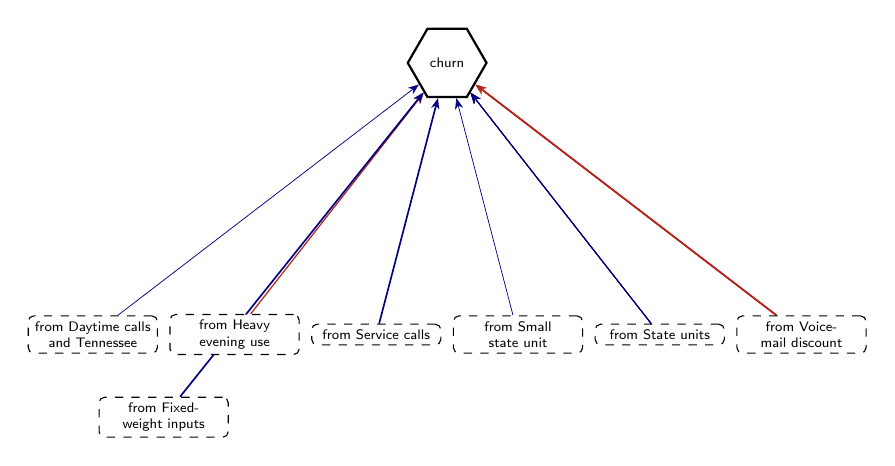
\begin{tikzpicture}[
  font=\sffamily\scriptsize, >={Stealth[length=1.4mm]},
  inp/.style={draw, circle, fill=white, minimum size=3.2mm, inner sep=0pt},
  hid/.style={draw, circle, fill=white, minimum size=5.2mm, inner sep=0.5pt, font=\sffamily\tiny},
  exitbox/.style={draw, thick, rectangle, fill=white, align=center, text width=17mm, minimum height=5mm, inner sep=1.5pt, font=\sffamily\tiny},
  sumbox/.style={draw, thick, dashed, rectangle, fill=white, align=center, text width=17mm, minimum height=5mm, inner sep=1.5pt, font=\sffamily\tiny},
  outp/.style={draw, thick, regular polygon, regular polygon sides=6, fill=white, minimum size=10mm, inner sep=0pt, font=\sffamily\tiny, align=center},
  stub/.style={draw, dashed, rounded corners=2pt, fill=white, align=center, inner sep=2pt, font=\sffamily\tiny, text width=15mm},
  inlab/.style={font=\sffamily\tiny, align=center, text width=15mm, inner sep=1pt, fill=white, fill opacity=0.8, text opacity=1},
  wpos/.style={draw=NavyBlue}, wneg/.style={draw=BrickRed}, wagg/.style={draw=black!45, line width=1.2pt},
  wmix/.style={draw=Plum},
]
\node[outp] (n0) at (5.4,3.45) {churn};
\node[stub] (nfromxxSmallxstatexunit) at (6.3,0.0) {from Small state unit};
\node[stub] (nfromxxHeavyxeveningxuse) at (2.7,0.0) {from Heavy evening use};
\node[stub] (nfromxxVoicemmailxdiscount) at (9.9,0.0) {from Voice-mail discount};
\node[stub] (nfromxxStatexunits) at (8.1,0.0) {from State units};
\node[stub] (nfromxxDaytimexcallsxandxTennessee) at (0.9,0.0) {from Daytime calls and Tennessee};
\node[stub] (nfromxxFixedmweightxinputs) at (1.8,-1.05) {from Fixed-weight inputs};
\node[stub] (nfromxxServicexcalls) at (4.5,0.0) {from Service calls};
\begin{scope}[on background layer]
\draw[->, wpos, line width=0.26pt] (nfromxxSmallxstatexunit) -- (n0);
\draw[->, wneg, line width=0.44pt] (nfromxxHeavyxeveningxuse) -- (n0);
\draw[->, wneg, line width=0.58pt] (nfromxxVoicemmailxdiscount) -- (n0);
\draw[->, wneg, line width=0.30pt] (nfromxxStatexunits) -- (n0);
\draw[->, wneg, line width=0.60pt] (nfromxxVoicemmailxdiscount) -- (n0);
\draw[->, wpos, line width=0.26pt] (nfromxxStatexunits) -- (n0);
\draw[->, wpos, line width=0.26pt] (nfromxxStatexunits) -- (n0);
\draw[->, wpos, line width=0.27pt] (nfromxxDaytimexcallsxandxTennessee) -- (n0);
\draw[->, wpos, line width=0.40pt] (nfromxxStatexunits) -- (n0);
\draw[->, wpos, line width=0.26pt] (nfromxxStatexunits) -- (n0);
\draw[->, wpos, line width=0.60pt] (nfromxxFixedmweightxinputs) -- (n0);
\draw[->, wpos, line width=0.60pt] (nfromxxServicexcalls) -- (n0);
\end{scope}
\end{tikzpicture}}%
\caption{The whole model: its units and every connection into them. Blue: positive weight (raises the score); red: negative weight (lowers it); thicker: larger weight. Orange outline and up arrow: raises the final prediction; teal and down arrow: lowers it; grey and double arrow: depends.}
\label{fig:churn100s2c1:units-ann102}
\end{figure}
\paragraph{Hypothesis.} The model adds up seven parts into one score: fixed-weight inputs, service calls, a voice-mail discount, heavy evening use, state units, a daytime-calls unit and a small state unit.\,{\scriptsize\textcolor{NavyBlue}{[C056]}}
\paragraph{Evidence.} It is made up of these seven parts (each explained below); the score is their sum, which was checked on all 4000 training customers.\,{\scriptsize\textcolor{NavyBlue}{[C056]}} Changing one input at a time across the whole model, an international plan takes a typical customer's chance of leaving from about 1\% to about 13\%, and a voice-mail plan lowers it to under 1\%.\,{\scriptsize\textcolor{NavyBlue}{[C001, C012]}} More customer-service calls raise it in an uneven way, from about 1\% at 0 calls to about 3\% at 3 calls.\,{\scriptsize\textcolor{NavyBlue}{[C008]}} The model ignores the daytime charge, evening calls, international calls and the night-time charge.\,{\scriptsize\textcolor{NavyBlue}{[C052, C053, C054, C055]}}
\par\noindent{\small Evidence plots: Figure~\ref{fig:churn100s2c1:plot-ann102-0}, Figure~\ref{fig:churn100s2c1:plot-ann102-1}.\par}
\begin{figure}[H]\centering
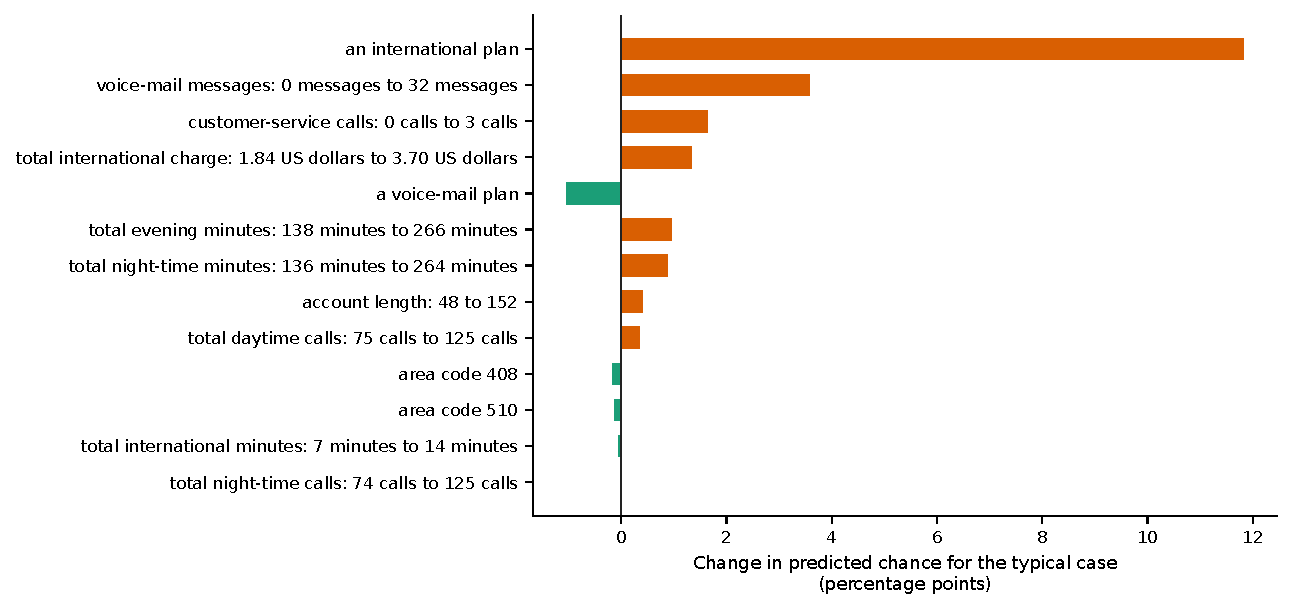
\includegraphics[width=\linewidth,height=0.88\textheight,keepaspectratio]{figures/churn100-s2-c1/ann_102-effects.pdf}
\caption{The whole model: Each input's change in the predicted value for the typical case across the whole model, largest first (orange: raises it, teal: lowers it).}
\label{fig:churn100s2c1:plot-ann102-0}
\end{figure}
\begin{figure}[H]\centering
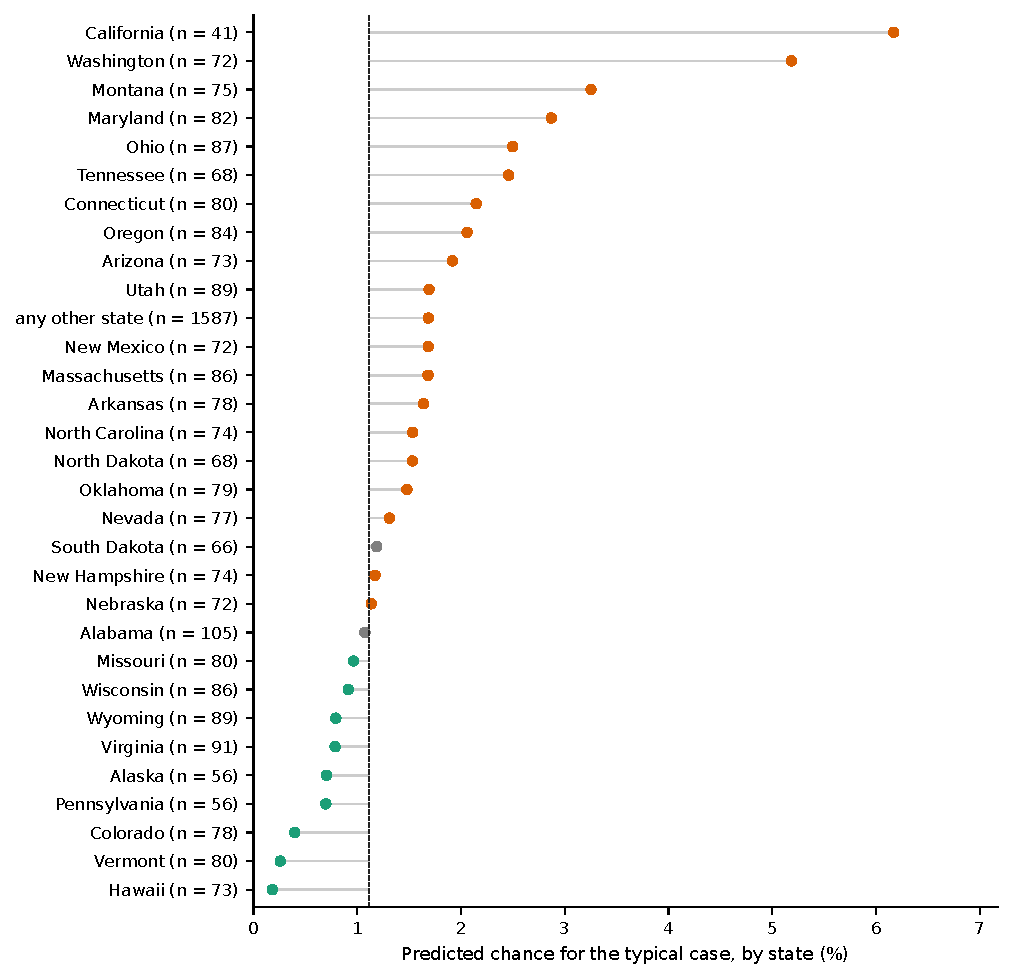
\includegraphics[width=\linewidth,height=0.88\textheight,keepaspectratio]{figures/churn100-s2-c1/ann_102-levels-state.pdf}
\caption{The whole model: Every level of state the model reads: the predicted value for the typical case at that level (dashed: the reference level); n = training customers; grey: few customers or not supported.}
\label{fig:churn100s2c1:plot-ann102-1}
\end{figure}
\par\smallskip\noindent{\small \textbf{Dive deeper:} Fixed-weight inputs (\ref{rd:ann99}); Service calls (\ref{rd:ann101}); Voice-mail discount (\ref{rd:ann95}); Heavy evening use (\ref{rd:ann94}); State units (\ref{rd:ann96}); Daytime calls and Tennessee (\ref{rd:ann97}); Small state unit (\ref{rd:ann92}). Technical detail: \ref{tech:ann102}.\par}
\subsubsection{Fixed-weight inputs}\label{rd:ann99}
\noindent{\footnotesize Part of: The whole model (\ref{rd:ann102}).\par}
\noindent{\small Figure~\ref{fig:churn100s2c1:parts-ann99} shows what feeds this part; Figure~\ref{fig:churn100s2c1:units-ann99} its units and every connection into them (dashed boxes: connections from or to other parts, drawn in their own sections).\par}
\begin{figure}[H]\centering
\resizebox{!}{\ifdim\height>0.5\textheight 0.5\textheight\else\height\fi}{%
\resizebox{\ifdim\width>\linewidth\linewidth\else\width\fi}{!}{%
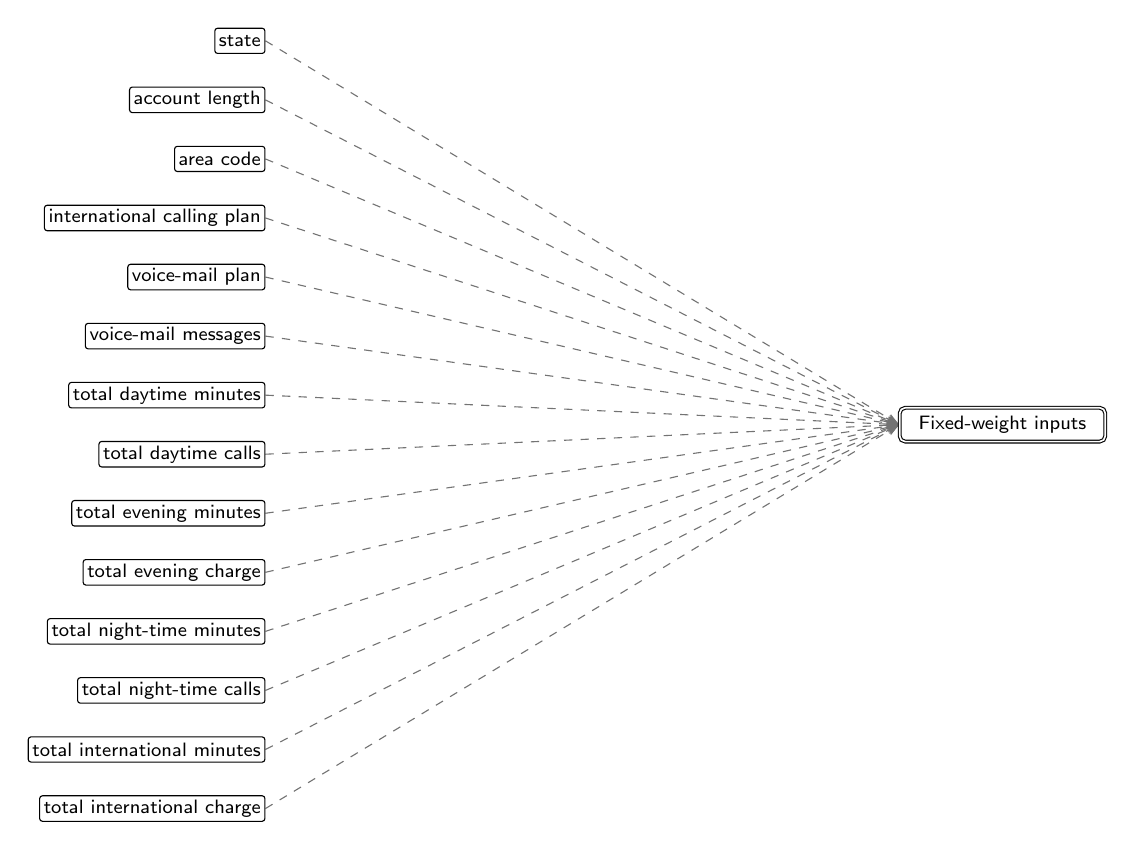
\begin{tikzpicture}[
  font=\sffamily\scriptsize, >={Stealth[length=1.6mm]},
  inp/.style={draw, rounded corners=1pt, fill=white, inner sep=1.5pt, minimum height=3.2mm, anchor=east},
  abox/.style={draw, thick, rounded corners=2pt, align=center, inner sep=3pt, minimum height=6mm, text width=42mm},
  outp/.style={draw, double, rounded corners=2pt, fill=white, align=center, inner sep=3pt, text width=24mm},
  agg/.style={draw=black!55},
]
\node[inp] (i0) at (0,4.875) {state};
\node[inp] (i1) at (0,4.125) {account length};
\node[inp] (i2) at (0,3.375) {area code};
\node[inp] (i3) at (0,2.625) {international calling plan};
\node[inp] (i4) at (0,1.875) {voice-mail plan};
\node[inp] (i5) at (0,1.125) {voice-mail messages};
\node[inp] (i6) at (0,0.375) {total daytime minutes};
\node[inp] (i7) at (0,-0.375) {total daytime calls};
\node[inp] (i8) at (0,-1.125) {total evening minutes};
\node[inp] (i9) at (0,-1.875) {total evening charge};
\node[inp] (i10) at (0,-2.625) {total night-time minutes};
\node[inp] (i11) at (0,-3.375) {total night-time calls};
\node[inp] (i12) at (0,-4.125) {total international minutes};
\node[inp] (i13) at (0,-4.875) {total international charge};
\node[outp] (out) at (9.36,0) {Fixed-weight inputs};
\begin{scope}[on background layer]
\draw[->, agg, thin, dashed] (i0.east) -- (out.west);
\draw[->, agg, thin, dashed] (i1.east) -- (out.west);
\draw[->, agg, thin, dashed] (i2.east) -- (out.west);
\draw[->, agg, thin, dashed] (i3.east) -- (out.west);
\draw[->, agg, thin, dashed] (i4.east) -- (out.west);
\draw[->, agg, thin, dashed] (i5.east) -- (out.west);
\draw[->, agg, thin, dashed] (i6.east) -- (out.west);
\draw[->, agg, thin, dashed] (i7.east) -- (out.west);
\draw[->, agg, thin, dashed] (i8.east) -- (out.west);
\draw[->, agg, thin, dashed] (i9.east) -- (out.west);
\draw[->, agg, thin, dashed] (i10.east) -- (out.west);
\draw[->, agg, thin, dashed] (i11.east) -- (out.west);
\draw[->, agg, thin, dashed] (i12.east) -- (out.west);
\draw[->, agg, thin, dashed] (i13.east) -- (out.west);
\end{scope}
\end{tikzpicture}}}%
\caption{Fixed-weight inputs: what feeds it, one level down.}
\label{fig:churn100s2c1:parts-ann99}
\end{figure}
\begin{figure}[H]\centering
\resizebox{\ifdim\width>\linewidth\linewidth\else\width\fi}{!}{%
\definecolor{netup}{HTML}{D95F02}\definecolor{netdown}{HTML}{1B9E77}\definecolor{netmixed}{HTML}{7F7F7F}%
\begin{tikzpicture}[
  font=\sffamily\scriptsize, >={Stealth[length=1.4mm]},
  inp/.style={draw, circle, fill=white, minimum size=3.2mm, inner sep=0pt},
  hid/.style={draw, circle, fill=white, minimum size=5.2mm, inner sep=0.5pt, font=\sffamily\tiny},
  exitbox/.style={draw, thick, rectangle, fill=white, align=center, text width=17mm, minimum height=5mm, inner sep=1.5pt, font=\sffamily\tiny},
  sumbox/.style={draw, thick, dashed, rectangle, fill=white, align=center, text width=17mm, minimum height=5mm, inner sep=1.5pt, font=\sffamily\tiny},
  outp/.style={draw, thick, regular polygon, regular polygon sides=6, fill=white, minimum size=10mm, inner sep=0pt, font=\sffamily\tiny, align=center},
  stub/.style={draw, dashed, rounded corners=2pt, fill=white, align=center, inner sep=2pt, font=\sffamily\tiny, text width=15mm},
  inlab/.style={font=\sffamily\tiny, align=center, text width=15mm, inner sep=1pt, fill=white, fill opacity=0.8, text opacity=1},
  wpos/.style={draw=NavyBlue}, wneg/.style={draw=BrickRed}, wagg/.style={draw=black!45, line width=1.2pt},
  wmix/.style={draw=Plum},
]
\node[exitbox] (nidentityxlin) at (5.85,1.9) {Fixed-weight inputs $\uparrow$};
\node[inp, draw=netmixed, very thick] (ngrpxxstate) at (4.5,0.0) {};
\path (ngrpxxstate.south) node[inlab, anchor=north] (labngrpxxstate) {state (31 of 51 used) $\updownarrow$};
\node[inp, draw=netup, very thick] (ninxxaccountxlength) at (0.9,-2.1) {};
\path (ninxxaccountxlength.south) node[inlab, anchor=north] (labninxxaccountxlength) {account length $\uparrow$};
\node[inp, draw=netdown, very thick] (ninxxareaxcodex408) at (2.7,0.0) {};
\path (ninxxareaxcodex408.south) node[inlab, anchor=north] (labninxxareaxcodex408) {area code 408 $\downarrow$};
\node[inp, draw=netup, very thick] (ninxxareaxcodex415) at (2.7,-2.1) {};
\path (ninxxareaxcodex415.south) node[inlab, anchor=north] (labninxxareaxcodex415) {area code 415 $\uparrow$};
\node[inp, draw=netdown, very thick] (ninxxareaxcodex510) at (3.6,-1.05) {};
\path (ninxxareaxcodex510.south) node[inlab, anchor=north] (labninxxareaxcodex510) {area code 510 $\downarrow$};
\node[inp, draw=netup, very thick] (ninxxinternationalxplan) at (1.8,-1.05) {};
\path (ninxxinternationalxplan.south) node[inlab, anchor=north] (labninxxinternationalxplan) {an international plan $\uparrow$};
\node[inp, draw=netup, very thick] (ninxxnumberxvmailxmessages) at (10.8,-1.05) {};
\path (ninxxnumberxvmailxmessages.south) node[inlab, anchor=north] (labninxxnumberxvmailxmessages) {voice-mail messages $\uparrow$};
\node[inp, draw=netup, very thick] (ninxxtotalxnightxminutes) at (9.9,0.0) {};
\path (ninxxtotalxnightxminutes.south) node[inlab, anchor=north] (labninxxtotalxnightxminutes) {total night-time minutes $\uparrow$};
\node[inp, draw=netdown, very thick] (ninxxtotalxnightxcalls) at (9.0,-1.05) {};
\path (ninxxtotalxnightxcalls.south) node[inlab, anchor=north] (labninxxtotalxnightxcalls) {total night-time calls $\downarrow$};
\node[inp, draw=netdown, very thick] (ninxxtotalxintlxminutes) at (8.1,0.0) {};
\path (ninxxtotalxintlxminutes.south) node[inlab, anchor=north] (labninxxtotalxintlxminutes) {total international minutes $\downarrow$};
\node[inp, draw=netup, very thick] (ninxxtotalxintlxcharge) at (7.2,-1.05) {};
\path (ninxxtotalxintlxcharge.south) node[inlab, anchor=north] (labninxxtotalxintlxcharge) {total international charge $\uparrow$};
\node[inp, draw=netup, very thick] (ninxxtotalxevexcharge) at (6.3,0.0) {};
\path (ninxxtotalxevexcharge.south) node[inlab, anchor=north] (labninxxtotalxevexcharge) {total evening charge $\uparrow$};
\node[inp, draw=netup, very thick] (ninxxtotalxevexminutes) at (6.3,-2.1) {};
\path (ninxxtotalxevexminutes.south) node[inlab, anchor=north] (labninxxtotalxevexminutes) {total evening minutes $\uparrow$};
\node[inp, draw=netup, very thick] (ninxxtotalxdayxcalls) at (4.5,-2.1) {};
\path (ninxxtotalxdayxcalls.south) node[inlab, anchor=north] (labninxxtotalxdayxcalls) {total daytime calls $\uparrow$};
\node[inp, draw=netup, very thick] (ninxxtotalxdayxminutes) at (5.4,-1.05) {};
\path (ninxxtotalxdayxminutes.south) node[inlab, anchor=north] (labninxxtotalxdayxminutes) {total daytime minutes $\uparrow$};
\node[inp, draw=netdown, very thick] (ninxxvoicexmailxplan) at (0.9,0.0) {};
\path (ninxxvoicexmailxplan.south) node[inlab, anchor=north] (labninxxvoicexmailxplan) {a voice-mail plan $\downarrow$};
\node[stub] (ntoxxthexmodelxoutput) at (5.85,3.45) {to the model output};
\begin{scope}[on background layer]
\node[fit=(nidentityxlin) , inner sep=8pt, rounded corners=5pt, fill=BurntOrange!10, draw=BurntOrange!45] (clu0) {};
\draw[->, wpos, line width=0.30pt] (ninxxaccountxlength) -- (nidentityxlin);
\draw[->, wneg, line width=0.26pt] (ninxxareaxcodex408) -- (nidentityxlin);
\draw[->, wpos, line width=0.27pt] (ninxxareaxcodex415) -- (nidentityxlin);
\draw[->, wneg, line width=0.26pt] (ninxxareaxcodex510) -- (nidentityxlin);
\draw[->, wpos, line width=0.51pt] (ninxxinternationalxplan) -- (nidentityxlin);
\draw[->, wpos, line width=0.47pt] (ninxxnumberxvmailxmessages) -- (nidentityxlin);
\draw[->, wpos, line width=0.36pt] (ninxxtotalxnightxminutes) -- (nidentityxlin);
\draw[->, wneg, line width=0.25pt] (ninxxtotalxnightxcalls) -- (nidentityxlin);
\draw[->, wneg, line width=0.26pt] (ninxxtotalxintlxminutes) -- (nidentityxlin);
\draw[->, wpos, line width=0.50pt] (ninxxtotalxintlxcharge) -- (nidentityxlin);
\draw[->, wpos, line width=0.41pt] (ninxxtotalxevexcharge) -- (nidentityxlin);
\draw[->, wpos, line width=0.43pt] (ninxxtotalxevexminutes) -- (nidentityxlin);
\draw[->, wpos, line width=0.29pt] (ninxxtotalxdayxcalls) -- (nidentityxlin);
\draw[->, wpos, line width=0.96pt] (ninxxtotalxdayxminutes) -- (nidentityxlin);
\draw[->, wneg, line width=0.56pt] (ninxxvoicexmailxplan) -- (nidentityxlin);
\draw[->, wpos, line width=0.60pt] (nidentityxlin) -- (ntoxxthexmodelxoutput);
\draw[->, wmix, line width=0.36pt] (ngrpxxstate) -- node[pos=0.8, sloped, above, font=\sffamily\tiny, inner sep=1pt, fill=white, fill opacity=0.8, text opacity=1] {25 edges, -0.30 to +0.15} (nidentityxlin);
\end{scope}
\node[font=\sffamily\scriptsize\bfseries, text=BurntOrange!55!black, anchor=south west, inner sep=1pt, fill=white, fill opacity=0.85, text opacity=1] at (clu0.north west) {Fixed-weight inputs};
\end{tikzpicture}}%
\caption{Fixed-weight inputs: its units and every connection into them. Blue: positive weight (raises the score); red: negative weight (lowers it); thicker: larger weight. Orange outline and up arrow: raises the final prediction; teal and down arrow: lowers it; grey and double arrow: depends.}
\label{fig:churn100s2c1:units-ann99}
\end{figure}
\paragraph{Hypothesis.} This part adds up most inputs with fixed weights: daytime minutes, an international plan and voice-mail messages raise the chance of leaving, steadily for the minutes and messages, and a voice-mail plan lowers it.\,{\scriptsize\textcolor{NavyBlue}{[C057, C058, C059, C067]}}
\paragraph{Evidence.} Through it, daytime minutes take a typical customer steadily from under 1\% at 112 to about 13\% at 249 minutes, and an international plan from about 1\% to about 13\%; a voice-mail plan lowers the chance to under 1\%.\,{\scriptsize\textcolor{NavyBlue}{[C057, C058, C067]}} The state moves it from about 1\% in West Virginia to about 4\% in California and Washington, and to under 1\% in Hawaii and Vermont.\,{\scriptsize\textcolor{NavyBlue}{[C060, C061, C066, C068]}} Its formula reproduces the part exactly on all 4000 training customers.\,{\scriptsize\textcolor{NavyBlue}{[C096]}}
\par\noindent{\small Evidence plots: Figure~\ref{fig:churn100s2c1:plot-ann99-0}, Figure~\ref{fig:churn100s2c1:plot-ann99-1}, Figure~\ref{fig:churn100s2c1:plot-ann99-2}, Figure~\ref{fig:churn100s2c1:plot-ann99-3}.\par}
\begin{figure}[H]\centering
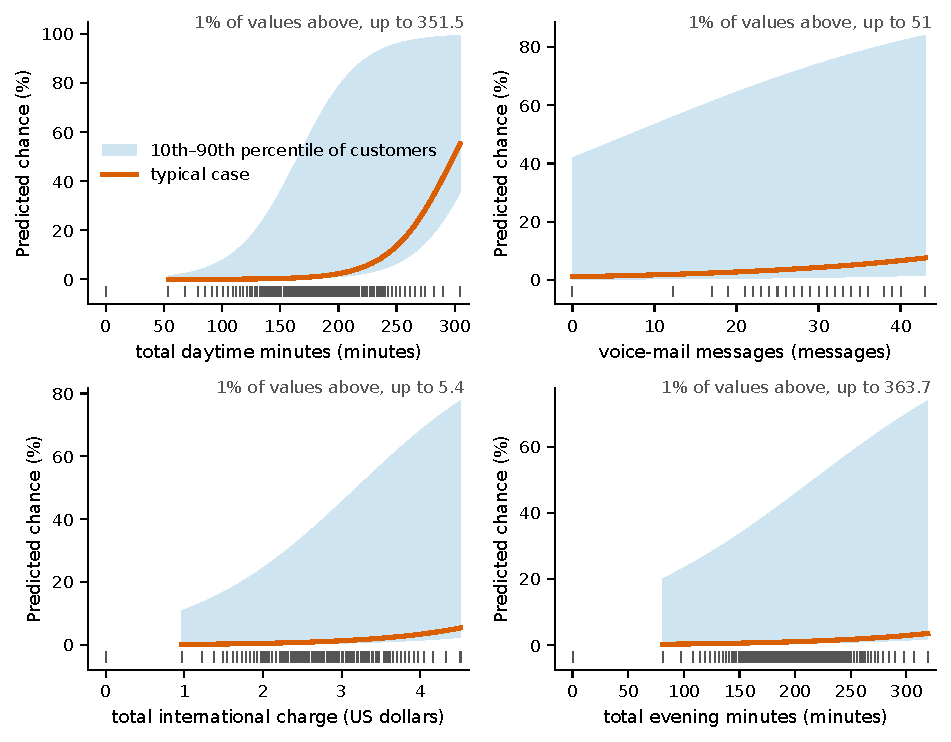
\includegraphics[width=\linewidth,height=0.88\textheight,keepaspectratio]{figures/churn100-s2-c1/ann_99-response.pdf}
\caption{Fixed-weight inputs: Response curves through this part: the typical case (bold), the 10th to 90th percentile of individual customers (band), the fold or step point (dashed) with its spread across them (grey), and the observed values (ticks).}
\label{fig:churn100s2c1:plot-ann99-0}
\end{figure}
\begin{figure}[H]\centering
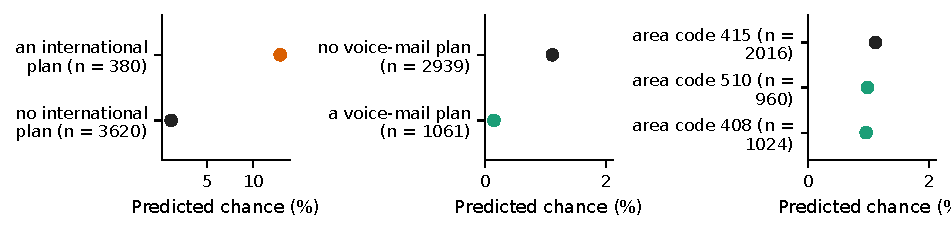
\includegraphics[width=\linewidth,height=0.88\textheight,keepaspectratio]{figures/churn100-s2-c1/ann_99-categories-small.pdf}
\caption{Fixed-weight inputs: The predicted value for the typical case at each level, through this part (n = training customers; grey: fewer than 20).}
\label{fig:churn100s2c1:plot-ann99-1}
\end{figure}
\begin{figure}[H]\centering
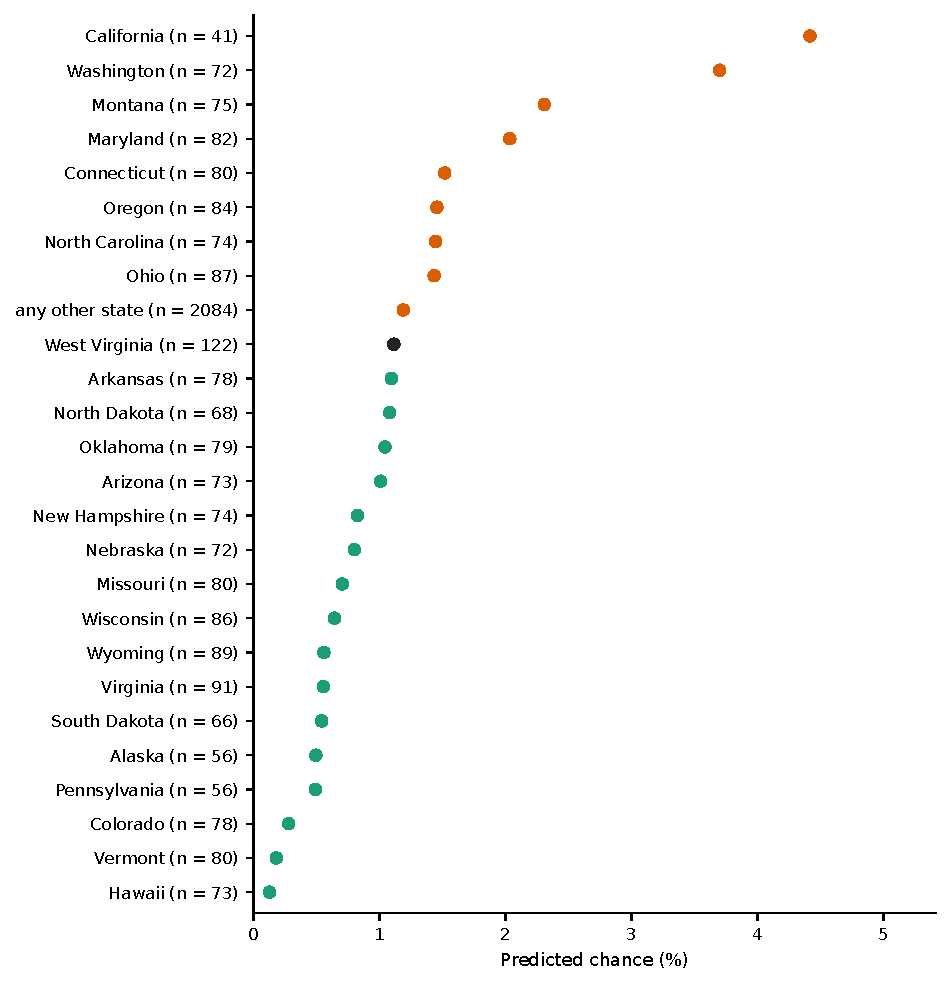
\includegraphics[width=\linewidth,height=0.88\textheight,keepaspectratio]{figures/churn100-s2-c1/ann_99-categories-C060.pdf}
\caption{Fixed-weight inputs: The predicted value for the typical case at each level, through this part (n = training customers; grey: fewer than 20).}
\label{fig:churn100s2c1:plot-ann99-2}
\end{figure}
\begin{figure}[H]\centering
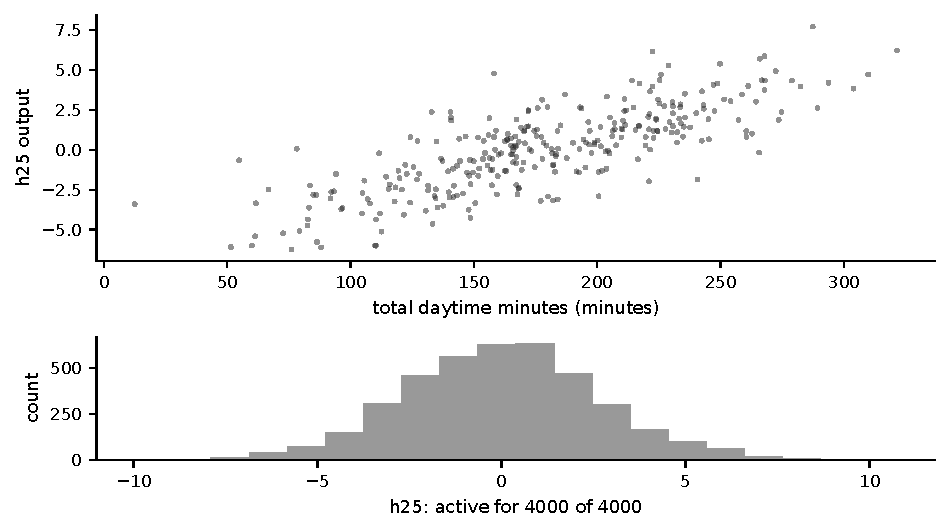
\includegraphics[width=\linewidth,height=0.88\textheight,keepaspectratio]{figures/churn100-s2-c1/ann_99-units.pdf}
\caption{Fixed-weight inputs: This part's hidden units: each unit's output against its main numeric input (top) and how often it is active (bottom).}
\label{fig:churn100s2c1:plot-ann99-3}
\end{figure}
\par\smallskip\noindent{\small Technical detail: \ref{tech:ann99}.\par}
\subsubsection{Service calls}\label{rd:ann101}
\noindent{\footnotesize Part of: The whole model (\ref{rd:ann102}).\par}
\noindent{\small Figure~\ref{fig:churn100s2c1:parts-ann101} shows what feeds this part; Figure~\ref{fig:churn100s2c1:units-ann101} its units and every connection into them (dashed boxes: connections from or to other parts, drawn in their own sections).\par}
\begin{figure}[H]\centering
\resizebox{!}{\ifdim\height>0.5\textheight 0.5\textheight\else\height\fi}{%
\resizebox{\ifdim\width>\linewidth\linewidth\else\width\fi}{!}{%
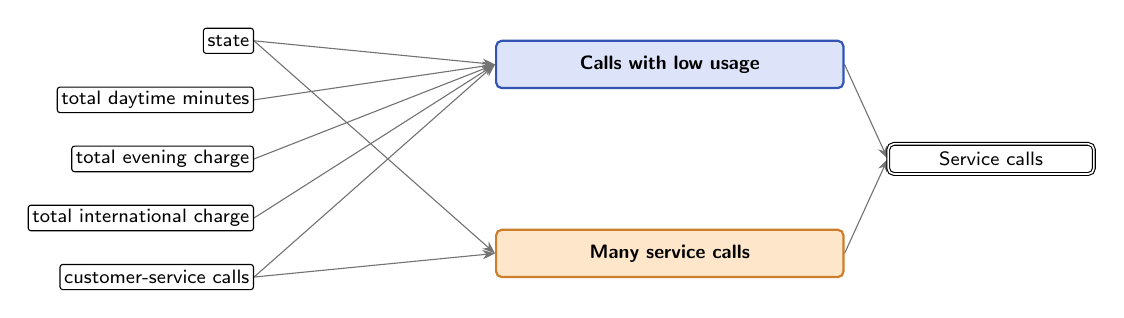
\begin{tikzpicture}[
  font=\sffamily\scriptsize, >={Stealth[length=1.6mm]},
  inp/.style={draw, rounded corners=1pt, fill=white, inner sep=1.5pt, minimum height=3.2mm, anchor=east},
  abox/.style={draw, thick, rounded corners=2pt, align=center, inner sep=3pt, minimum height=6mm, text width=42mm},
  outp/.style={draw, double, rounded corners=2pt, fill=white, align=center, inner sep=3pt, text width=24mm},
  agg/.style={draw=black!55},
]
\node[inp] (i0) at (0,1.5) {state};
\node[inp] (i1) at (0,0.75) {total daytime minutes};
\node[inp] (i2) at (0,-0.0) {total evening charge};
\node[inp] (i3) at (0,-0.75) {total international charge};
\node[inp] (i4) at (0,-1.5) {customer-service calls};
\node[abox, fill=RoyalBlue!18, draw=RoyalBlue!80!black] (b0) at (5.28,1.2) {\textbf{Calls with low usage}};
\node[abox, fill=BurntOrange!18, draw=BurntOrange!80!black] (b1) at (5.28,-1.2) {\textbf{Many service calls}};
\node[outp] (out) at (9.36,0) {Service calls};
\begin{scope}[on background layer]
\draw[->, agg, thin] (i0.east) -- (b0.west);
\draw[->, agg, thin] (i1.east) -- (b0.west);
\draw[->, agg, thin] (i2.east) -- (b0.west);
\draw[->, agg, thin] (i3.east) -- (b0.west);
\draw[->, agg, thin] (i4.east) -- (b0.west);
\draw[->, agg] (b0.east) -- (out.west);
\draw[->, agg, thin] (i0.east) -- (b1.west);
\draw[->, agg, thin] (i4.east) -- (b1.west);
\draw[->, agg] (b1.east) -- (out.west);
\end{scope}
\end{tikzpicture}}}%
\caption{Service calls: what feeds it, one level down.}
\label{fig:churn100s2c1:parts-ann101}
\end{figure}
\begin{figure}[H]\centering
\resizebox{\ifdim\width>\linewidth\linewidth\else\width\fi}{!}{%
\definecolor{netup}{HTML}{D95F02}\definecolor{netdown}{HTML}{1B9E77}\definecolor{netmixed}{HTML}{7F7F7F}%
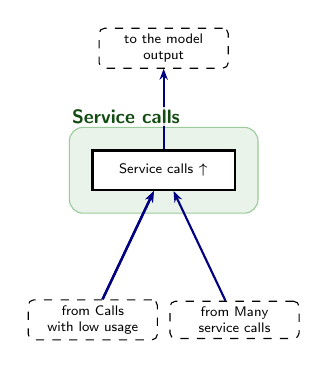
\begin{tikzpicture}[
  font=\sffamily\scriptsize, >={Stealth[length=1.4mm]},
  inp/.style={draw, circle, fill=white, minimum size=3.2mm, inner sep=0pt},
  hid/.style={draw, circle, fill=white, minimum size=5.2mm, inner sep=0.5pt, font=\sffamily\tiny},
  exitbox/.style={draw, thick, rectangle, fill=white, align=center, text width=17mm, minimum height=5mm, inner sep=1.5pt, font=\sffamily\tiny},
  sumbox/.style={draw, thick, dashed, rectangle, fill=white, align=center, text width=17mm, minimum height=5mm, inner sep=1.5pt, font=\sffamily\tiny},
  outp/.style={draw, thick, regular polygon, regular polygon sides=6, fill=white, minimum size=10mm, inner sep=0pt, font=\sffamily\tiny, align=center},
  stub/.style={draw, dashed, rounded corners=2pt, fill=white, align=center, inner sep=2pt, font=\sffamily\tiny, text width=15mm},
  inlab/.style={font=\sffamily\tiny, align=center, text width=15mm, inner sep=1pt, fill=white, fill opacity=0.8, text opacity=1},
  wpos/.style={draw=NavyBlue}, wneg/.style={draw=BrickRed}, wagg/.style={draw=black!45, line width=1.2pt},
  wmix/.style={draw=Plum},
]
\node[exitbox] (nidentityxsvc) at (1.8,1.9) {Service calls $\uparrow$};
\node[stub] (nfromxxCallsxwithxlowxusage) at (0.9,0.0) {from Calls with low usage};
\node[stub] (nfromxxManyxservicexcalls) at (2.7,0.0) {from Many service calls};
\node[stub] (ntoxxthexmodelxoutput) at (1.8,3.45) {to the model output};
\begin{scope}[on background layer]
\node[fit=(nidentityxsvc) , inner sep=8pt, rounded corners=5pt, fill=ForestGreen!10, draw=ForestGreen!45] (clu0) {};
\draw[->, wpos, line width=0.81pt] (nfromxxCallsxwithxlowxusage) -- (nidentityxsvc);
\draw[->, wpos, line width=0.88pt] (nfromxxCallsxwithxlowxusage) -- (nidentityxsvc);
\draw[->, wpos, line width=0.77pt] (nfromxxManyxservicexcalls) -- (nidentityxsvc);
\draw[->, wpos, line width=0.60pt] (nidentityxsvc) -- (ntoxxthexmodelxoutput);
\end{scope}
\node[font=\sffamily\scriptsize\bfseries, text=ForestGreen!55!black, anchor=south west, inner sep=1pt, fill=white, fill opacity=0.85, text opacity=1] at (clu0.north west) {Service calls};
\end{tikzpicture}}%
\caption{Service calls: its units and every connection into them. Blue: positive weight (raises the score); red: negative weight (lowers it); thicker: larger weight. Orange outline and up arrow: raises the final prediction; teal and down arrow: lowers it; grey and double arrow: depends.}
\label{fig:churn100s2c1:units-ann101}
\end{figure}
\paragraph{Hypothesis.} This part raises the chance of leaving with calls to customer service, from 4 calls upwards and in an uneven way, and more so for customers with low daytime use; it adds up two parts.\,{\scriptsize\textcolor{NavyBlue}{[C111, C108, C107]}}
\paragraph{Evidence.} It is made of two parts that are added: calls with low usage, and many service calls.\,{\scriptsize\textcolor{NavyBlue}{[C111]}} Through it, daytime minutes lower a typical customer's chance only while they stay below about 170 minutes (between 147 and 216 minutes for different customers), in an uneven way, from about 38\% at 91 minutes to about 1\% at 352 minutes.\,{\scriptsize\textcolor{NavyBlue}{[C107]}} Customer-service calls add to it from 4 calls upwards, in an uneven way: for a typical such customer, from about 3\% at 0 calls to about 11\% at 4 calls.\,{\scriptsize\textcolor{NavyBlue}{[C108]}} With an evening charge above 17.12 US dollars, the chance is lowest at about 154 minutes of daytime use and higher either side: from about 1\% at 112 minutes to about 17\% at 249 minutes, against about 2\% to about 10\% at or below that charge.\,{\scriptsize\textcolor{NavyBlue}{[C103]}}
\par\noindent{\small Evidence plots: Figure~\ref{fig:churn100s2c1:plot-ann101-0}, Figure~\ref{fig:churn100s2c1:plot-ann101-1}, Figure~\ref{fig:churn100s2c1:plot-ann101-2}, Figure~\ref{fig:churn100s2c1:plot-ann101-3}, Figure~\ref{fig:churn100s2c1:plot-ann101-4}, Figure~\ref{fig:churn100s2c1:plot-ann101-5}, Figure~\ref{fig:churn100s2c1:plot-ann101-6}, Figure~\ref{fig:churn100s2c1:plot-ann101-7}.\par}
\par\noindent{\small Figure~\ref{fig:churn100s2c1:plot-ann101-6} shows this part's own output, unit h26: over its two main inputs, with the line where it switches on.\par}
\begin{figure}[H]\centering
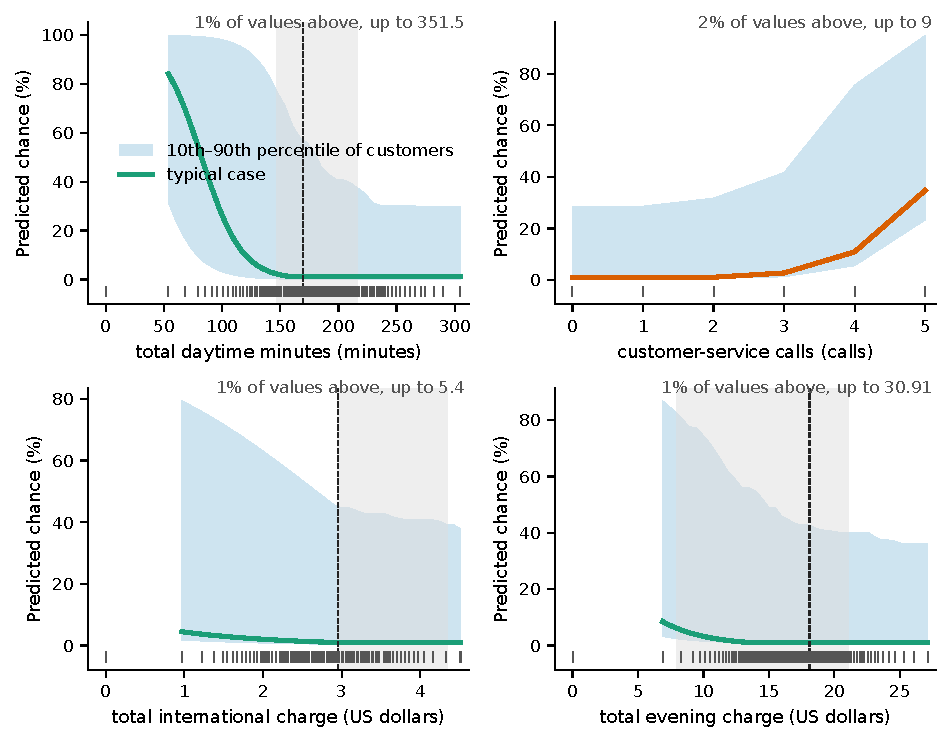
\includegraphics[width=\linewidth,height=0.88\textheight,keepaspectratio]{figures/churn100-s2-c1/ann_101-response.pdf}
\caption{Service calls: Response curves through this part: the typical case (bold), the 10th to 90th percentile of individual customers (band), the fold or step point (dashed) with its spread across them (grey), and the observed values (ticks).}
\label{fig:churn100s2c1:plot-ann101-0}
\end{figure}
\begin{figure}[H]\centering
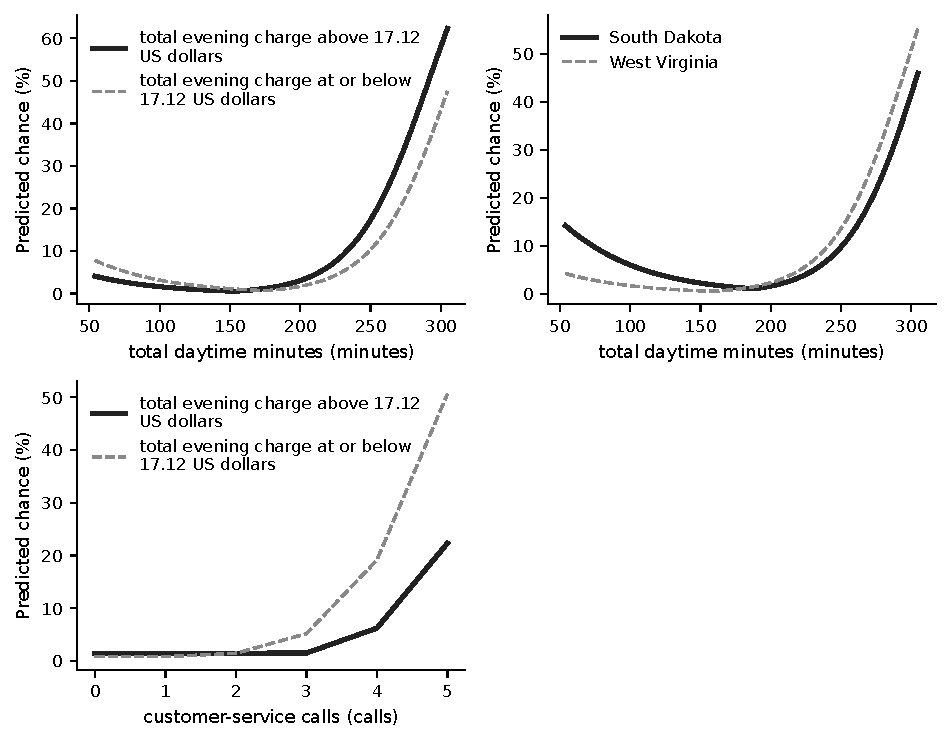
\includegraphics[width=\linewidth,height=0.88\textheight,keepaspectratio]{figures/churn100-s2-c1/ann_101-interaction.pdf}
\caption{Service calls: How the effect differs between groups: one curve per group, for the typical case of each group.}
\label{fig:churn100s2c1:plot-ann101-1}
\end{figure}
\begin{figure}[H]\centering
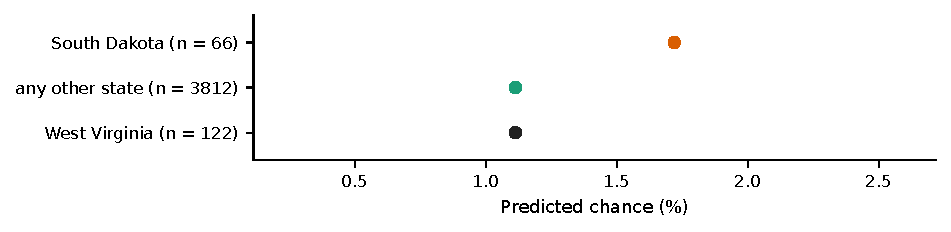
\includegraphics[width=\linewidth,height=0.88\textheight,keepaspectratio]{figures/churn100-s2-c1/ann_101-categories-small.pdf}
\caption{Service calls: The predicted value for the typical case at each level, through this part (n = training customers; grey: fewer than 20).}
\label{fig:churn100s2c1:plot-ann101-2}
\end{figure}
\begin{figure}[H]\centering
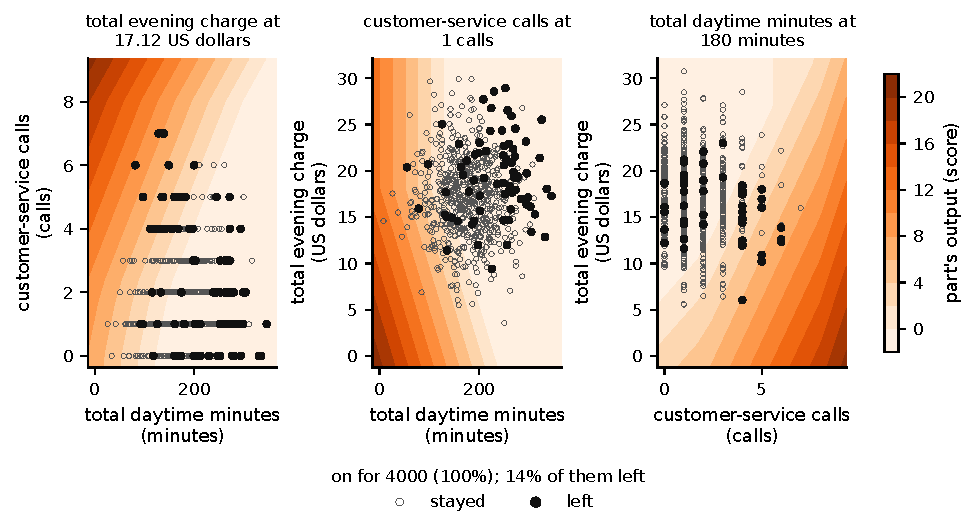
\includegraphics[width=\linewidth,height=0.88\textheight,keepaspectratio]{figures/churn100-s2-c1/ann_101-deep-map.pdf}
\caption{Service calls: The part's own output over each pair of its three main inputs (the third held at its median, named above each panel; the points are the training rows whose third input is between its 40th and 60th percentile), other inputs at the typical case: colour where it is on, flat grey where it is switched off, the black line where it switches on; training customers as hollow (no event) and filled (event) points, so the part can be seen catching the events (the predicted-chance overlay was harder to read). The switch-on line is traced on this map only; the boundary claim (C162) did not pass its check on the data, so no rule is stated.}
\label{fig:churn100s2c1:plot-ann101-3}
\end{figure}
\begin{figure}[H]\centering
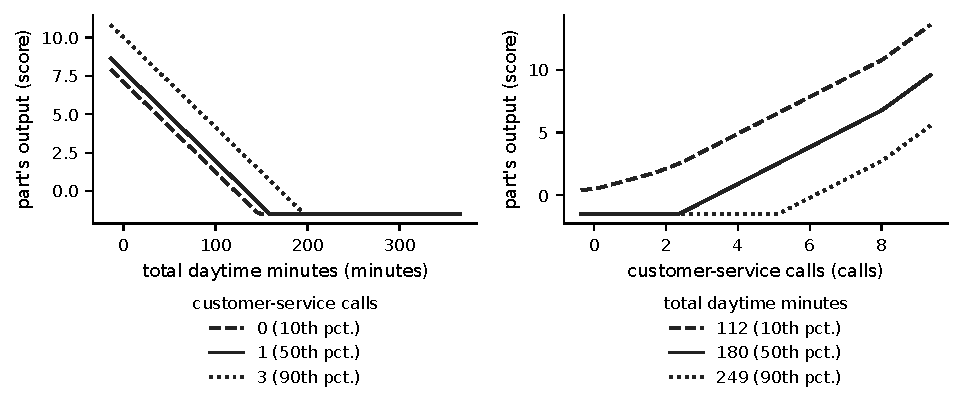
\includegraphics[width=\linewidth,height=0.88\textheight,keepaspectratio]{figures/churn100-s2-c1/ann_101-deep-slices.pdf}
\caption{Service calls: Slices of the same map: the part's own output against each input at three values of the other, so the tilted boundary shows as a shifting hinge. The switch-on line is traced on this map only; the boundary claim (C162) did not pass its check on the data, so no rule is stated.}
\label{fig:churn100s2c1:plot-ann101-4}
\end{figure}
\begin{figure}[H]\centering
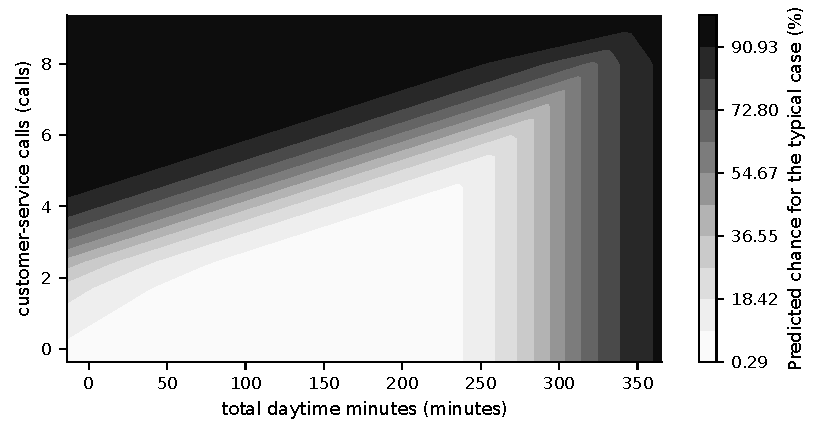
\includegraphics[width=\linewidth,height=0.88\textheight,keepaspectratio]{figures/churn100-s2-c1/ann_101-deep-risk.pdf}
\caption{Service calls: The same map on the final scale: the predicted value for the typical case, with the switch-on line (orange). The switch-on line is traced on this map only; the boundary claim (C162) did not pass its check on the data, so no rule is stated.}
\label{fig:churn100s2c1:plot-ann101-5}
\end{figure}
\begin{figure}[H]\centering
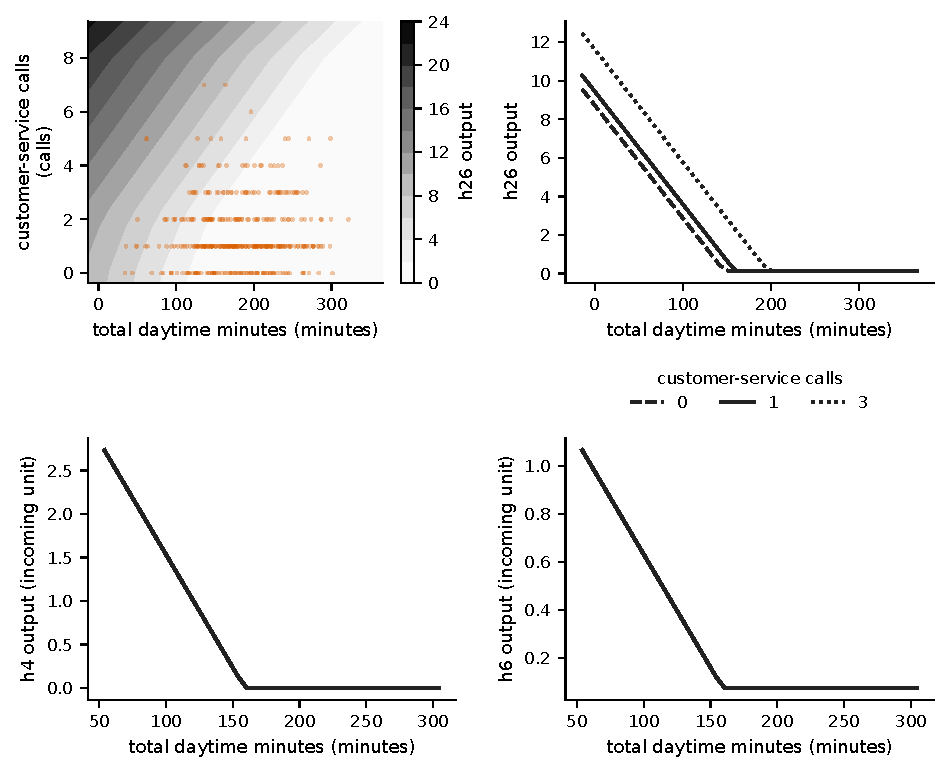
\includegraphics[width=\linewidth,height=0.88\textheight,keepaspectratio]{figures/churn100-s2-c1/ann_101-partial-identity_svc.pdf}
\caption{Service calls: This part's own output, unit h26 (combines 3 non-linear units), on its own scale (its activation), with every other input at the typical case; it is active for 3145 of 4000. Left: its output over its two main inputs (orange line: where it switches on; dots: the data); right: slices at three values of the second input; then each incoming non-linear unit against its own main input.}
\label{fig:churn100s2c1:plot-ann101-6}
\end{figure}
\begin{figure}[H]\centering
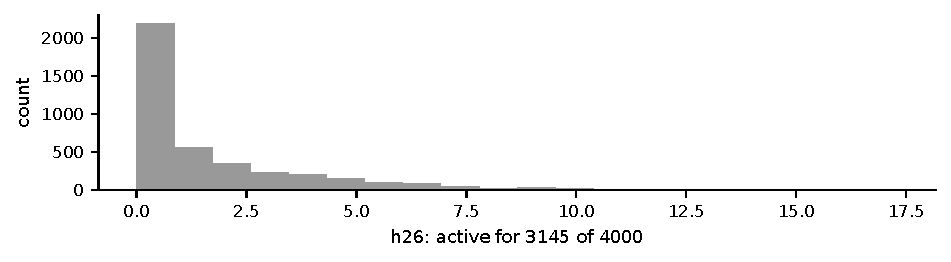
\includegraphics[width=\linewidth,height=0.88\textheight,keepaspectratio]{figures/churn100-s2-c1/ann_101-units.pdf}
\caption{Service calls: This part's hidden units: each unit's output against its main numeric input (top) and how often it is active (bottom).}
\label{fig:churn100s2c1:plot-ann101-7}
\end{figure}
\par\smallskip\noindent{\small \textbf{Dive deeper:} Calls with low usage (\ref{rd:ann91}); Many service calls (\ref{rd:ann93}). Technical detail: \ref{tech:ann101}.\par}
\subsubsection{Calls with low usage}\label{rd:ann91}
\noindent{\footnotesize Part of: Service calls (\ref{rd:ann101}).\par}
\noindent{\small Figure~\ref{fig:churn100s2c1:parts-ann91} shows what feeds this part; Figure~\ref{fig:churn100s2c1:units-ann91} its units and every connection into them (dashed boxes: connections from or to other parts, drawn in their own sections).\par}
\begin{figure}[H]\centering
\resizebox{!}{\ifdim\height>0.5\textheight 0.5\textheight\else\height\fi}{%
\resizebox{\ifdim\width>\linewidth\linewidth\else\width\fi}{!}{%
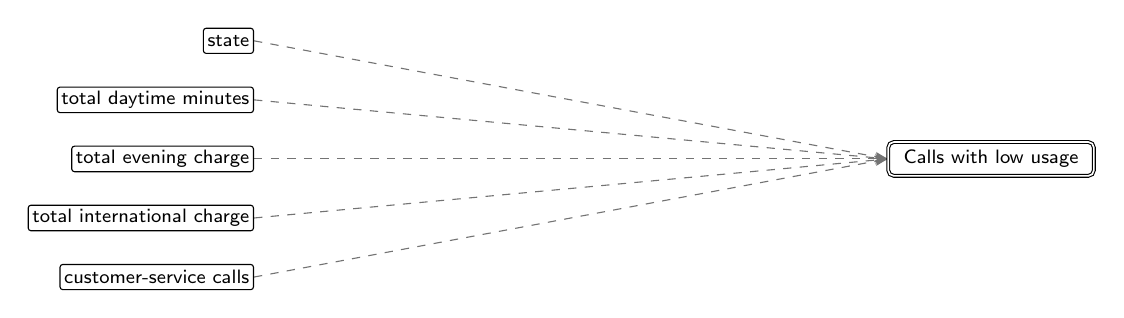
\begin{tikzpicture}[
  font=\sffamily\scriptsize, >={Stealth[length=1.6mm]},
  inp/.style={draw, rounded corners=1pt, fill=white, inner sep=1.5pt, minimum height=3.2mm, anchor=east},
  abox/.style={draw, thick, rounded corners=2pt, align=center, inner sep=3pt, minimum height=6mm, text width=42mm},
  outp/.style={draw, double, rounded corners=2pt, fill=white, align=center, inner sep=3pt, text width=24mm},
  agg/.style={draw=black!55},
]
\node[inp] (i0) at (0,1.5) {state};
\node[inp] (i1) at (0,0.75) {total daytime minutes};
\node[inp] (i2) at (0,-0.0) {total evening charge};
\node[inp] (i3) at (0,-0.75) {total international charge};
\node[inp] (i4) at (0,-1.5) {customer-service calls};
\node[outp] (out) at (9.36,0) {Calls with low usage};
\begin{scope}[on background layer]
\draw[->, agg, thin, dashed] (i0.east) -- (out.west);
\draw[->, agg, thin, dashed] (i1.east) -- (out.west);
\draw[->, agg, thin, dashed] (i2.east) -- (out.west);
\draw[->, agg, thin, dashed] (i3.east) -- (out.west);
\draw[->, agg, thin, dashed] (i4.east) -- (out.west);
\end{scope}
\end{tikzpicture}}}%
\caption{Calls with low usage: what feeds it, one level down.}
\label{fig:churn100s2c1:parts-ann91}
\end{figure}
\begin{figure}[H]\centering
\resizebox{\ifdim\width>\linewidth\linewidth\else\width\fi}{!}{%
\definecolor{netup}{HTML}{D95F02}\definecolor{netdown}{HTML}{1B9E77}\definecolor{netmixed}{HTML}{7F7F7F}%
\begin{tikzpicture}[
  font=\sffamily\scriptsize, >={Stealth[length=1.4mm]},
  inp/.style={draw, circle, fill=white, minimum size=3.2mm, inner sep=0pt},
  hid/.style={draw, circle, fill=white, minimum size=5.2mm, inner sep=0.5pt, font=\sffamily\tiny},
  exitbox/.style={draw, thick, rectangle, fill=white, align=center, text width=17mm, minimum height=5mm, inner sep=1.5pt, font=\sffamily\tiny},
  sumbox/.style={draw, thick, dashed, rectangle, fill=white, align=center, text width=17mm, minimum height=5mm, inner sep=1.5pt, font=\sffamily\tiny},
  outp/.style={draw, thick, regular polygon, regular polygon sides=6, fill=white, minimum size=10mm, inner sep=0pt, font=\sffamily\tiny, align=center},
  stub/.style={draw, dashed, rounded corners=2pt, fill=white, align=center, inner sep=2pt, font=\sffamily\tiny, text width=15mm},
  inlab/.style={font=\sffamily\tiny, align=center, text width=15mm, inner sep=1pt, fill=white, fill opacity=0.8, text opacity=1},
  wpos/.style={draw=NavyBlue}, wneg/.style={draw=BrickRed}, wagg/.style={draw=black!45, line width=1.2pt},
  wmix/.style={draw=Plum},
]
\node[hid] (n9555xb) at (5.25,1.9) {h24};
\node[hid] (n2627xb) at (3.75,3.25) {h22};
\node[hid] (n2796) at (5.25,3.25) {h7};
\node[hid] (n12926) at (3.75,1.9) {h17};
\node[hid] (n1264) at (4.5,5.95) {h6};
\node[hid] (n807) at (4.5,4.6) {h4};
\node[inp, draw=netdown, very thick] (ninxxtotalxintlxcharge) at (4.5,0.0) {};
\path (ninxxtotalxintlxcharge.south) node[inlab, anchor=north] (labninxxtotalxintlxcharge) {total international charge $\downarrow$};
\node[inp, draw=netdown, very thick] (ninxxtotalxevexcharge) at (8.1,0.0) {};
\path (ninxxtotalxevexcharge.south) node[inlab, anchor=north] (labninxxtotalxevexcharge) {total evening charge $\downarrow$};
\node[inp, draw=netdown, very thick] (ninxxtotalxdayxminutes) at (2.7,0.0) {};
\path (ninxxtotalxdayxminutes.south) node[inlab, anchor=north] (labninxxtotalxdayxminutes) {total daytime minutes $\downarrow$};
\node[inp, draw=netmixed, very thick] (ngrpxxstate) at (6.3,0.0) {};
\path (ngrpxxstate.south) node[inlab, anchor=north] (labngrpxxstate) {state (31 of 51 used) $\updownarrow$};
\node[inp, draw=netup, very thick] (ninxxnumberxcustomerxservicexcalls) at (0.9,0.0) {};
\path (ninxxnumberxcustomerxservicexcalls.south) node[inlab, anchor=north] (labninxxnumberxcustomerxservicexcalls) {customer-service calls $\uparrow$};
\node[stub] (ntoxxServicexcalls) at (4.5,7.5) {to Service calls};
\begin{scope}[on background layer]
\node[fit=(n9555xb) (n2627xb) (n2796) (n12926) (n1264) (n807) , inner sep=8pt, rounded corners=5pt, fill=ForestGreen!10, draw=ForestGreen!45] (clu0) {};
\draw[->, wpos, line width=0.47pt] (n2796) -- (n807);
\draw[->, wpos, line width=0.38pt] (n807) -- (n1264);
\draw[->, wpos, line width=0.37pt] (n12926) -- (n2796);
\draw[->, wpos, line width=0.49pt] (n2627xb) -- (n807);
\draw[->, wpos, line width=0.36pt] (n9555xb) -- (n2627xb);
\draw[->, wneg, line width=0.36pt] (ninxxtotalxintlxcharge) -- (n1264);
\draw[->, wneg, line width=0.60pt] (ninxxtotalxevexcharge) -- (n2796);
\draw[->, wneg, line width=0.74pt] (ninxxtotalxdayxminutes) -- (n807);
\draw[->, wpos, line width=0.26pt] (ninxxnumberxcustomerxservicexcalls) -- (n807);
\draw[->, wpos, line width=0.38pt] (ninxxnumberxcustomerxservicexcalls) -- (n2796);
\draw[->, wpos, line width=0.60pt] (ninxxnumberxcustomerxservicexcalls) -- (n12926);
\draw[->, wpos, line width=0.35pt] (ninxxnumberxcustomerxservicexcalls) -- (n2627xb);
\draw[->, wpos, line width=0.55pt] (ninxxnumberxcustomerxservicexcalls) -- (n9555xb);
\draw[->, wpos, line width=0.81pt] (n807) -- (ntoxxServicexcalls);
\draw[->, wpos, line width=0.88pt] (n1264) -- (ntoxxServicexcalls);
\draw[->, wpos, line width=0.30pt] (ngrpxxstate) -- node[pos=0.8, sloped, above, font=\sffamily\tiny, inner sep=1pt, fill=white, fill opacity=0.8, text opacity=1] {+0.15} (n2796);
\end{scope}
\node[font=\sffamily\scriptsize\bfseries, text=ForestGreen!55!black, anchor=south west, inner sep=1pt, fill=white, fill opacity=0.85, text opacity=1] at (clu0.north west) {Calls with low usage};
\end{tikzpicture}}%
\caption{Calls with low usage: its units and every connection into them. Blue: positive weight (raises the score); red: negative weight (lowers it); thicker: larger weight. Orange outline and up arrow: raises the final prediction; teal and down arrow: lowers it; grey and double arrow: depends.}
\label{fig:churn100s2c1:units-ann91}
\end{figure}
\paragraph{Hypothesis.} This part raises the chance of leaving for customers with low usage, more so when they call customer service: daytime minutes lower it only while they stay below about 170 minutes (between 147 and 216 minutes for different customers), and calls raise it, both in an uneven way.\,{\scriptsize\textcolor{NavyBlue}{[C119, C113]}}
\paragraph{Evidence.} It acts on 3121 of 4000 training customers, 402 of whom left; for the typical customer it acts on, it changes the chance by less than a point.\,{\scriptsize\textcolor{NavyBlue}{[C123]}} Through it, a typical customer's chance falls in an uneven way from about 38\% at 91 minutes of daytime use to about 1\% at 352 minutes, with no further fall past about 170 minutes (between 147 and 216 minutes for different customers).\,{\scriptsize\textcolor{NavyBlue}{[C119]}} A higher international charge lowers it only while it stays below about 2.95 US dollars (between 2.95 and 4.34 US dollars for different customers), in an uneven way, from about 3\% to about 1\%.\,{\scriptsize\textcolor{NavyBlue}{[C121]}} Customer-service calls raise it in an uneven way, from about 1\% at 0 calls to about 3\% at 3 calls.\,{\scriptsize\textcolor{NavyBlue}{[C113]}} Its formula reproduces the part exactly on all 4000 training customers.\,{\scriptsize\textcolor{NavyBlue}{[C124]}}
\par\noindent{\small Evidence plots: Figure~\ref{fig:churn100s2c1:plot-ann91-0}, Figure~\ref{fig:churn100s2c1:plot-ann91-1}, Figure~\ref{fig:churn100s2c1:plot-ann91-2}, Figure~\ref{fig:churn100s2c1:plot-ann91-3}, Figure~\ref{fig:churn100s2c1:plot-ann91-4}, Figure~\ref{fig:churn100s2c1:plot-ann91-5}, Figure~\ref{fig:churn100s2c1:plot-ann91-6}, Figure~\ref{fig:churn100s2c1:plot-ann91-7}, Figure~\ref{fig:churn100s2c1:plot-ann91-8}.\par}
\par\noindent{\small Figure~\ref{fig:churn100s2c1:plot-ann91-6} shows this part's own output, unit h4: over its two main inputs, with the line where it switches on.\par}
\par\noindent{\small Figure~\ref{fig:churn100s2c1:plot-ann91-7} shows this part's own output, unit h6: over its two main inputs, with the line where it switches on.\par}
\begin{figure}[H]\centering
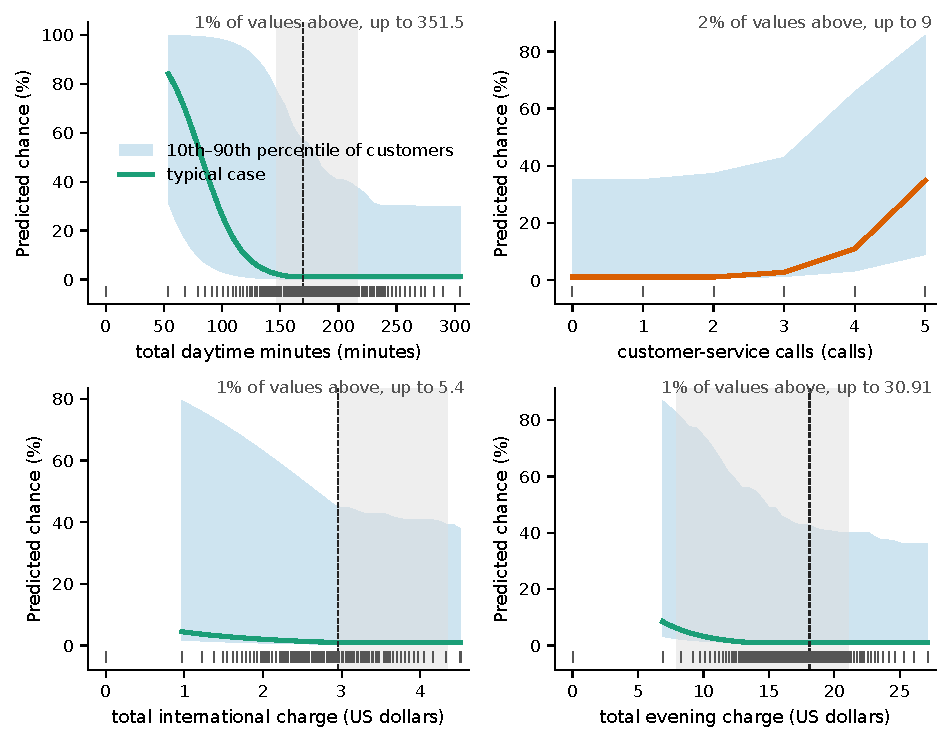
\includegraphics[width=\linewidth,height=0.88\textheight,keepaspectratio]{figures/churn100-s2-c1/ann_91-response.pdf}
\caption{Calls with low usage: Response curves through this part: the typical case (bold), the 10th to 90th percentile of individual customers (band), the fold or step point (dashed) with its spread across them (grey), and the observed values (ticks).}
\label{fig:churn100s2c1:plot-ann91-0}
\end{figure}
\begin{figure}[H]\centering
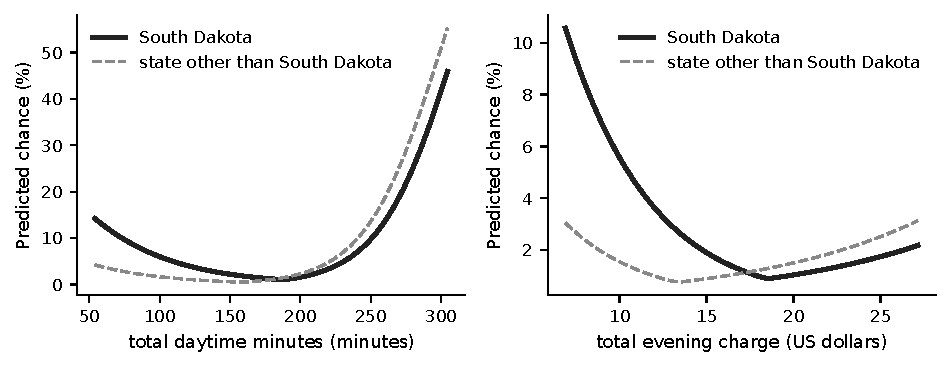
\includegraphics[width=\linewidth,height=0.88\textheight,keepaspectratio]{figures/churn100-s2-c1/ann_91-interaction.pdf}
\caption{Calls with low usage: How the effect differs between groups: one curve per group, for the typical case of each group.}
\label{fig:churn100s2c1:plot-ann91-1}
\end{figure}
\begin{figure}[H]\centering
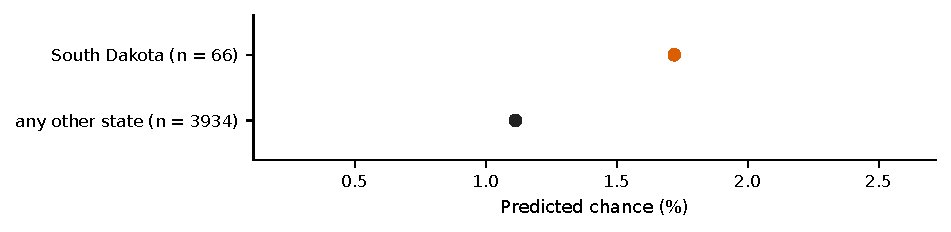
\includegraphics[width=\linewidth,height=0.88\textheight,keepaspectratio]{figures/churn100-s2-c1/ann_91-categories-small.pdf}
\caption{Calls with low usage: The predicted value for the typical case at each level, through this part (n = training customers; grey: fewer than 20).}
\label{fig:churn100s2c1:plot-ann91-2}
\end{figure}
\begin{figure}[H]\centering
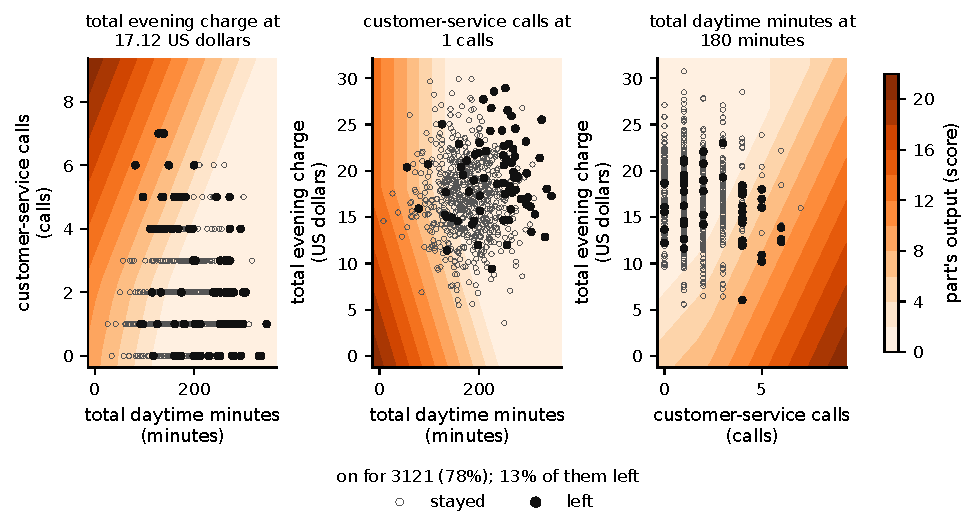
\includegraphics[width=\linewidth,height=0.88\textheight,keepaspectratio]{figures/churn100-s2-c1/ann_91-deep-map.pdf}
\caption{Calls with low usage: The part's own output over each pair of its three main inputs (the third held at its median, named above each panel; the points are the training rows whose third input is between its 40th and 60th percentile), other inputs at the typical case: colour where it is on, flat grey where it is switched off, the black line where it switches on; training customers as hollow (no event) and filled (event) points, so the part can be seen catching the events (the predicted-chance overlay was harder to read). The switch-on line is traced on this map only; the boundary claim (C163) did not pass its check on the data, so no rule is stated.}
\label{fig:churn100s2c1:plot-ann91-3}
\end{figure}
\begin{figure}[H]\centering
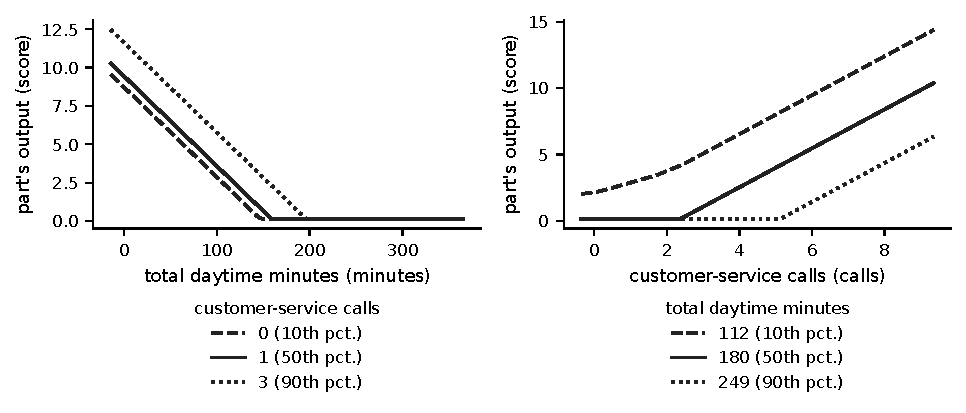
\includegraphics[width=\linewidth,height=0.88\textheight,keepaspectratio]{figures/churn100-s2-c1/ann_91-deep-slices.pdf}
\caption{Calls with low usage: Slices of the same map: the part's own output against each input at three values of the other, so the tilted boundary shows as a shifting hinge. The switch-on line is traced on this map only; the boundary claim (C163) did not pass its check on the data, so no rule is stated.}
\label{fig:churn100s2c1:plot-ann91-4}
\end{figure}
\begin{figure}[H]\centering
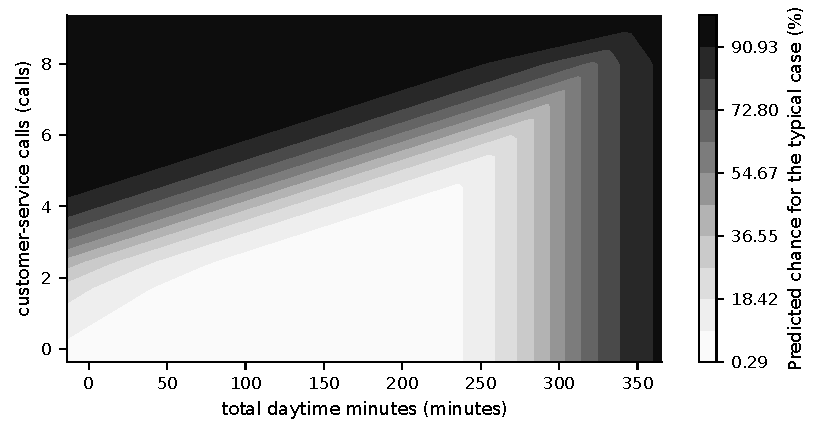
\includegraphics[width=\linewidth,height=0.88\textheight,keepaspectratio]{figures/churn100-s2-c1/ann_91-deep-risk.pdf}
\caption{Calls with low usage: The same map on the final scale: the predicted value for the typical case, with the switch-on line (orange). The switch-on line is traced on this map only; the boundary claim (C163) did not pass its check on the data, so no rule is stated.}
\label{fig:churn100s2c1:plot-ann91-5}
\end{figure}
\begin{figure}[H]\centering
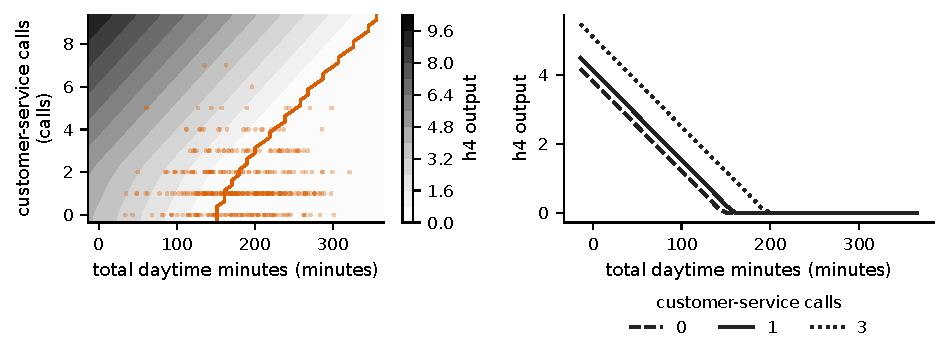
\includegraphics[width=\linewidth,height=0.88\textheight,keepaspectratio]{figures/churn100-s2-c1/ann_91-partial-807.pdf}
\caption{Calls with low usage: This part's own output, unit h4 (the output of 'Calls with low usage'), on its own scale (its activation), with every other input at the typical case; it is active for 1840 of 4000. Left: its output over its two main inputs (orange line: where it switches on; dots: the data); right: slices at three values of the second input.}
\label{fig:churn100s2c1:plot-ann91-6}
\end{figure}
\begin{figure}[H]\centering
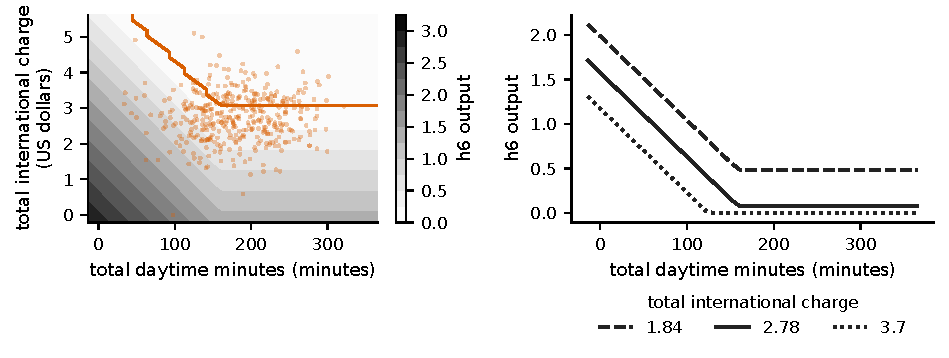
\includegraphics[width=\linewidth,height=0.88\textheight,keepaspectratio]{figures/churn100-s2-c1/ann_91-partial-1264.pdf}
\caption{Calls with low usage: This part's own output, unit h6 (the output of 'Calls with low usage'), on its own scale (its activation), with every other input at the typical case; it is active for 2901 of 4000. Left: its output over its two main inputs (orange line: where it switches on; dots: the data); right: slices at three values of the second input.}
\label{fig:churn100s2c1:plot-ann91-7}
\end{figure}
\begin{figure}[H]\centering
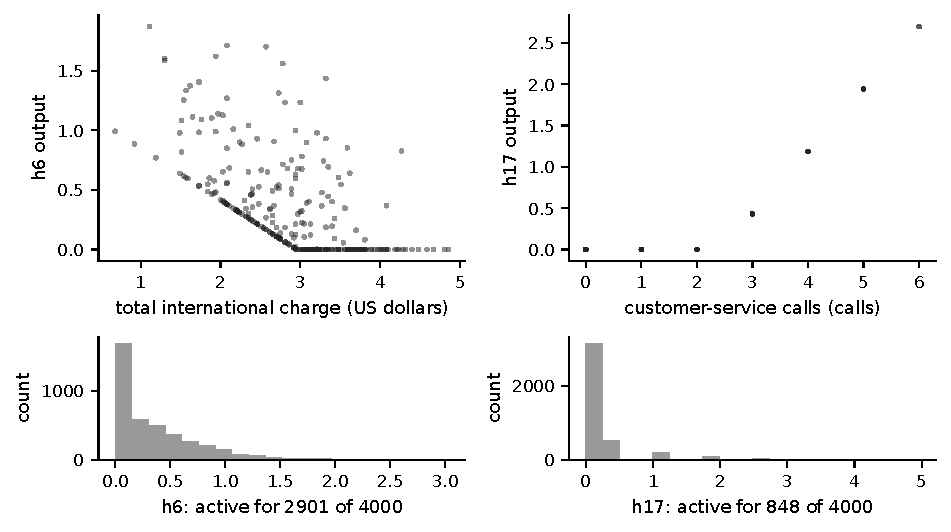
\includegraphics[width=\linewidth,height=0.88\textheight,keepaspectratio]{figures/churn100-s2-c1/ann_91-units.pdf}
\caption{Calls with low usage: This part's hidden units: each unit's output against its main numeric input (top) and how often it is active (bottom).}
\label{fig:churn100s2c1:plot-ann91-8}
\end{figure}
\par\smallskip\noindent{\small Technical detail: \ref{tech:ann91}.\par}
\subsubsection{Many service calls}\label{rd:ann93}
\noindent{\footnotesize Part of: Service calls (\ref{rd:ann101}).\par}
\noindent{\small Figure~\ref{fig:churn100s2c1:parts-ann93} shows what feeds this part; Figure~\ref{fig:churn100s2c1:units-ann93} its units and every connection into them (dashed boxes: connections from or to other parts, drawn in their own sections).\par}
\begin{figure}[H]\centering
\resizebox{!}{\ifdim\height>0.5\textheight 0.5\textheight\else\height\fi}{%
\resizebox{\ifdim\width>\linewidth\linewidth\else\width\fi}{!}{%
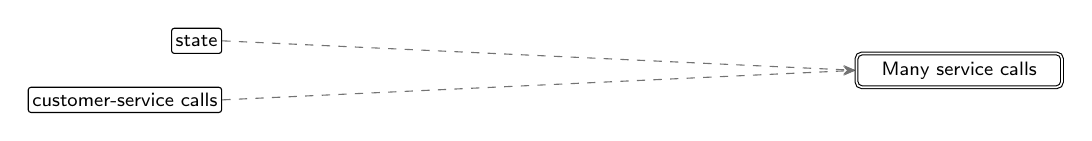
\begin{tikzpicture}[
  font=\sffamily\scriptsize, >={Stealth[length=1.6mm]},
  inp/.style={draw, rounded corners=1pt, fill=white, inner sep=1.5pt, minimum height=3.2mm, anchor=east},
  abox/.style={draw, thick, rounded corners=2pt, align=center, inner sep=3pt, minimum height=6mm, text width=42mm},
  outp/.style={draw, double, rounded corners=2pt, fill=white, align=center, inner sep=3pt, text width=24mm},
  agg/.style={draw=black!55},
]
\node[inp] (i0) at (0,0.375) {state};
\node[inp] (i1) at (0,-0.375) {customer-service calls};
\node[outp] (out) at (9.36,0) {Many service calls};
\begin{scope}[on background layer]
\draw[->, agg, thin, dashed] (i0.east) -- (out.west);
\draw[->, agg, thin, dashed] (i1.east) -- (out.west);
\end{scope}
\end{tikzpicture}}}%
\caption{Many service calls: what feeds it, one level down.}
\label{fig:churn100s2c1:parts-ann93}
\end{figure}
\begin{figure}[H]\centering
\resizebox{\ifdim\width>\linewidth\linewidth\else\width\fi}{!}{%
\definecolor{netup}{HTML}{D95F02}\definecolor{netdown}{HTML}{1B9E77}\definecolor{netmixed}{HTML}{7F7F7F}%
\begin{tikzpicture}[
  font=\sffamily\scriptsize, >={Stealth[length=1.4mm]},
  inp/.style={draw, circle, fill=white, minimum size=3.2mm, inner sep=0pt},
  hid/.style={draw, circle, fill=white, minimum size=5.2mm, inner sep=0.5pt, font=\sffamily\tiny},
  exitbox/.style={draw, thick, rectangle, fill=white, align=center, text width=17mm, minimum height=5mm, inner sep=1.5pt, font=\sffamily\tiny},
  sumbox/.style={draw, thick, dashed, rectangle, fill=white, align=center, text width=17mm, minimum height=5mm, inner sep=1.5pt, font=\sffamily\tiny},
  outp/.style={draw, thick, regular polygon, regular polygon sides=6, fill=white, minimum size=10mm, inner sep=0pt, font=\sffamily\tiny, align=center},
  stub/.style={draw, dashed, rounded corners=2pt, fill=white, align=center, inner sep=2pt, font=\sffamily\tiny, text width=15mm},
  inlab/.style={font=\sffamily\tiny, align=center, text width=15mm, inner sep=1pt, fill=white, fill opacity=0.8, text opacity=1},
  wpos/.style={draw=NavyBlue}, wneg/.style={draw=BrickRed}, wagg/.style={draw=black!45, line width=1.2pt},
  wmix/.style={draw=Plum},
]
\node[hid] (n17032) at (1.8,1.9) {h20};
\node[exitbox] (n7208) at (1.8,3.25) {Many service calls $\uparrow$};
\node[inp, draw=netup, very thick] (ninxxnumberxcustomerxservicexcalls) at (0.9,0.0) {};
\path (ninxxnumberxcustomerxservicexcalls.south) node[inlab, anchor=north] (labninxxnumberxcustomerxservicexcalls) {customer-service calls $\uparrow$};
\node[inp, draw=netmixed, very thick] (ngrpxxstate) at (2.7,0.0) {};
\path (ngrpxxstate.south) node[inlab, anchor=north] (labngrpxxstate) {state (31 of 51 used) $\updownarrow$};
\node[stub] (ntoxxServicexcalls) at (1.8,4.8) {to Service calls};
\begin{scope}[on background layer]
\node[fit=(n17032) (n7208) , inner sep=8pt, rounded corners=5pt, fill=ForestGreen!10, draw=ForestGreen!45] (clu0) {};
\draw[->, wpos, line width=0.44pt] (n17032) -- (n7208);
\draw[->, wpos, line width=0.60pt] (ninxxnumberxcustomerxservicexcalls) -- (n17032);
\draw[->, wpos, line width=0.77pt] (n7208) -- (ntoxxServicexcalls);
\draw[->, wneg, line width=0.38pt] (ngrpxxstate) -- node[pos=0.8, sloped, above, font=\sffamily\tiny, inner sep=1pt, fill=white, fill opacity=0.8, text opacity=1] {-0.36} (n7208);
\end{scope}
\node[font=\sffamily\scriptsize\bfseries, text=ForestGreen!55!black, anchor=south west, inner sep=1pt, fill=white, fill opacity=0.85, text opacity=1] at (clu0.north west) {Many service calls};
\end{tikzpicture}}%
\caption{Many service calls: its units and every connection into them. Blue: positive weight (raises the score); red: negative weight (lowers it); thicker: larger weight. Orange outline and up arrow: raises the final prediction; teal and down arrow: lowers it; grey and double arrow: depends.}
\label{fig:churn100s2c1:units-ann93}
\end{figure}
\paragraph{Hypothesis.} This part raises the chance of leaving with calls to customer service, adding nothing until about 3 calls, then steadily, except in West Virginia.\,{\scriptsize\textcolor{NavyBlue}{[C131, C130]}}
\paragraph{Evidence.} It acts on 306 of 4000 training customers, 154 of whom left; for the typical customer it acts on, the chance is about 16\% without it and about 26\% with it.\,{\scriptsize\textcolor{NavyBlue}{[C132]}} It is switched off in West Virginia: for the typical customer it acts on, being in any other state takes the chance from about 16\% to about 26\%.\,{\scriptsize\textcolor{NavyBlue}{[C130]}} Its formula reproduces the part exactly on all 4000 training customers.\,{\scriptsize\textcolor{NavyBlue}{[C133]}}
\par\noindent{\small Evidence plots: Figure~\ref{fig:churn100s2c1:plot-ann93-0}, Figure~\ref{fig:churn100s2c1:plot-ann93-1}, Figure~\ref{fig:churn100s2c1:plot-ann93-2}.\par}
\par\noindent{\small Figure~\ref{fig:churn100s2c1:plot-ann93-1} shows this part's own output, unit h12.\par}
\begin{figure}[H]\centering
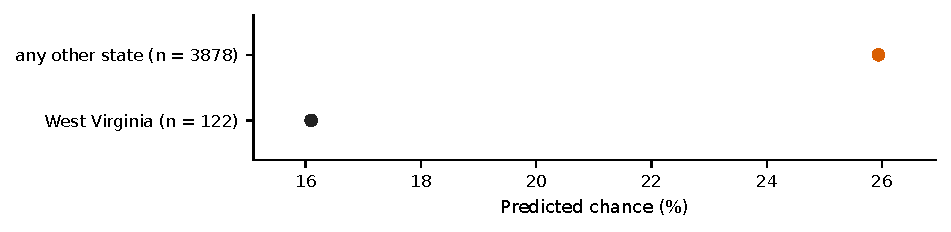
\includegraphics[width=\linewidth,height=0.88\textheight,keepaspectratio]{figures/churn100-s2-c1/ann_93-categories-small.pdf}
\caption{Many service calls: The predicted value for the typical case at each level, through this part (n = training customers; grey: fewer than 20).}
\label{fig:churn100s2c1:plot-ann93-0}
\end{figure}
\begin{figure}[H]\centering
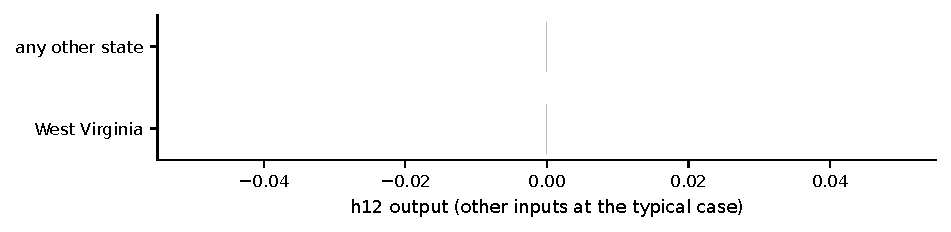
\includegraphics[width=\linewidth,height=0.88\textheight,keepaspectratio]{figures/churn100-s2-c1/ann_93-partial-7208.pdf}
\caption{Many service calls: This part's own output, unit h12 (the output of 'Many service calls'), on its own scale (its activation), with every other input at the typical case; it is active for 306 of 4000. Its output for each combination of the levels it reads.}
\label{fig:churn100s2c1:plot-ann93-1}
\end{figure}
\begin{figure}[H]\centering
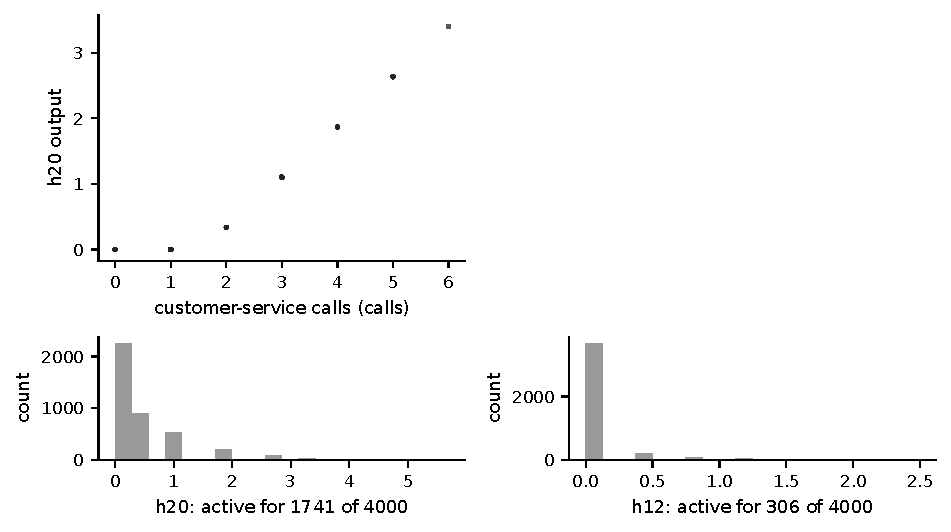
\includegraphics[width=\linewidth,height=0.88\textheight,keepaspectratio]{figures/churn100-s2-c1/ann_93-units.pdf}
\caption{Many service calls: This part's hidden units: each unit's output against its main numeric input (top) and how often it is active (bottom).}
\label{fig:churn100s2c1:plot-ann93-2}
\end{figure}
\par\smallskip\noindent{\small Technical detail: \ref{tech:ann93}.\par}
\subsubsection{Voice-mail discount}\label{rd:ann95}
\noindent{\footnotesize Part of: The whole model (\ref{rd:ann102}).\par}
\noindent{\small Figure~\ref{fig:churn100s2c1:parts-ann95} shows what feeds this part; Figure~\ref{fig:churn100s2c1:units-ann95} its units and every connection into them (dashed boxes: connections from or to other parts, drawn in their own sections).\par}
\begin{figure}[H]\centering
\resizebox{!}{\ifdim\height>0.5\textheight 0.5\textheight\else\height\fi}{%
\resizebox{\ifdim\width>\linewidth\linewidth\else\width\fi}{!}{%
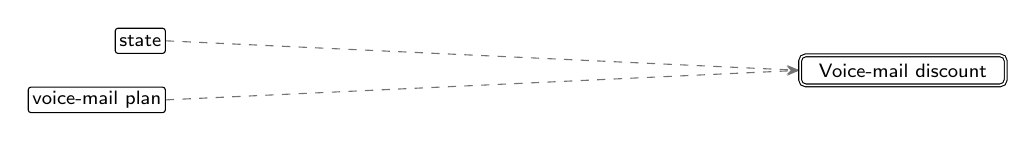
\begin{tikzpicture}[
  font=\sffamily\scriptsize, >={Stealth[length=1.6mm]},
  inp/.style={draw, rounded corners=1pt, fill=white, inner sep=1.5pt, minimum height=3.2mm, anchor=east},
  abox/.style={draw, thick, rounded corners=2pt, align=center, inner sep=3pt, minimum height=6mm, text width=42mm},
  outp/.style={draw, double, rounded corners=2pt, fill=white, align=center, inner sep=3pt, text width=24mm},
  agg/.style={draw=black!55},
]
\node[inp] (i0) at (0,0.375) {state};
\node[inp] (i1) at (0,-0.375) {voice-mail plan};
\node[outp] (out) at (9.36,0) {Voice-mail discount};
\begin{scope}[on background layer]
\draw[->, agg, thin, dashed] (i0.east) -- (out.west);
\draw[->, agg, thin, dashed] (i1.east) -- (out.west);
\end{scope}
\end{tikzpicture}}}%
\caption{Voice-mail discount: what feeds it, one level down.}
\label{fig:churn100s2c1:parts-ann95}
\end{figure}
\begin{figure}[H]\centering
\resizebox{\ifdim\width>\linewidth\linewidth\else\width\fi}{!}{%
\definecolor{netup}{HTML}{D95F02}\definecolor{netdown}{HTML}{1B9E77}\definecolor{netmixed}{HTML}{7F7F7F}%
\begin{tikzpicture}[
  font=\sffamily\scriptsize, >={Stealth[length=1.4mm]},
  inp/.style={draw, circle, fill=white, minimum size=3.2mm, inner sep=0pt},
  hid/.style={draw, circle, fill=white, minimum size=5.2mm, inner sep=0.5pt, font=\sffamily\tiny},
  exitbox/.style={draw, thick, rectangle, fill=white, align=center, text width=17mm, minimum height=5mm, inner sep=1.5pt, font=\sffamily\tiny},
  sumbox/.style={draw, thick, dashed, rectangle, fill=white, align=center, text width=17mm, minimum height=5mm, inner sep=1.5pt, font=\sffamily\tiny},
  outp/.style={draw, thick, regular polygon, regular polygon sides=6, fill=white, minimum size=10mm, inner sep=0pt, font=\sffamily\tiny, align=center},
  stub/.style={draw, dashed, rounded corners=2pt, fill=white, align=center, inner sep=2pt, font=\sffamily\tiny, text width=15mm},
  inlab/.style={font=\sffamily\tiny, align=center, text width=15mm, inner sep=1pt, fill=white, fill opacity=0.8, text opacity=1},
  wpos/.style={draw=NavyBlue}, wneg/.style={draw=BrickRed}, wagg/.style={draw=black!45, line width=1.2pt},
  wmix/.style={draw=Plum},
]
\node[hid] (n5577) at (1.9,1.9) {h10};
\node[hid] (n1133) at (1.9,3.25) {h5};
\node[hid] (n4051) at (1.9,4.6) {h9};
\node[inp, draw=netmixed, very thick] (ngrpxxstate) at (1.0,0.0) {};
\path (ngrpxxstate.south) node[inlab, anchor=north] (labngrpxxstate) {state (31 of 51 used) $\updownarrow$};
\node[inp, draw=netdown, very thick] (ninxxvoicexmailxplan) at (2.8,0.0) {};
\path (ninxxvoicexmailxplan.south) node[inlab, anchor=north] (labninxxvoicexmailxplan) {a voice-mail plan $\downarrow$};
\node[stub] (ntoxxthexmodelxoutput) at (1.9,6.15) {to the model output};
\begin{scope}[on background layer]
\node[fit=(n5577) (n1133) (n4051) , inner sep=8pt, rounded corners=5pt, fill=Orchid!10, draw=Orchid!45] (clu0) {};
\draw[->, wpos, line width=0.65pt] (n1133) -- (n4051);
\draw[->, wpos, line width=0.30pt] (n5577) -- (n1133);
\draw[->, wpos, line width=0.60pt] (ninxxvoicexmailxplan) -- (n5577);
\draw[->, wneg, line width=0.58pt] (n1133) -- (ntoxxthexmodelxoutput);
\draw[->, wneg, line width=0.60pt] (n4051) -- (ntoxxthexmodelxoutput);
\draw[->, wpos, line width=0.34pt] (ngrpxxstate) -- node[pos=0.8, sloped, above, font=\sffamily\tiny, inner sep=1pt, fill=white, fill opacity=0.8, text opacity=1] {+0.26} (n5577);
\draw[->, wpos, line width=0.27pt] (ngrpxxstate) -- node[pos=0.8, sloped, above, font=\sffamily\tiny, inner sep=1pt, fill=white, fill opacity=0.8, text opacity=1] {+0.06} (n4051);
\draw[->, wpos, line width=0.26pt] (ngrpxxstate) -- node[pos=0.8, sloped, above, font=\sffamily\tiny, inner sep=1pt, fill=white, fill opacity=0.8, text opacity=1] {+0.02} (n1133);
\end{scope}
\node[font=\sffamily\scriptsize\bfseries, text=Orchid!55!black, anchor=south west, inner sep=1pt, fill=white, fill opacity=0.85, text opacity=1] at (clu0.north west) {Voice-mail discount};
\end{tikzpicture}}%
\caption{Voice-mail discount: its units and every connection into them. Blue: positive weight (raises the score); red: negative weight (lowers it); thicker: larger weight. Orange outline and up arrow: raises the final prediction; teal and down arrow: lowers it; grey and double arrow: depends.}
\label{fig:churn100s2c1:units-ann95}
\end{figure}
\paragraph{Hypothesis.} This part gives customers with a voice-mail plan a small discount on the chance of leaving.\,{\scriptsize\textcolor{NavyBlue}{[C125]}}
\paragraph{Evidence.} Through it, a voice-mail plan lowers a typical customer's chance by less than a point, and customers in states other than Alabama, North Carolina and West Virginia get about 2\% instead of about 1\%.\,{\scriptsize\textcolor{NavyBlue}{[C125, C126]}} Its formula reproduces the part exactly on all 4000 training customers.\,{\scriptsize\textcolor{NavyBlue}{[C129]}}
\par\noindent{\small Evidence plots: Figure~\ref{fig:churn100s2c1:plot-ann95-0}, Figure~\ref{fig:churn100s2c1:plot-ann95-1}.\par}
\begin{figure}[H]\centering
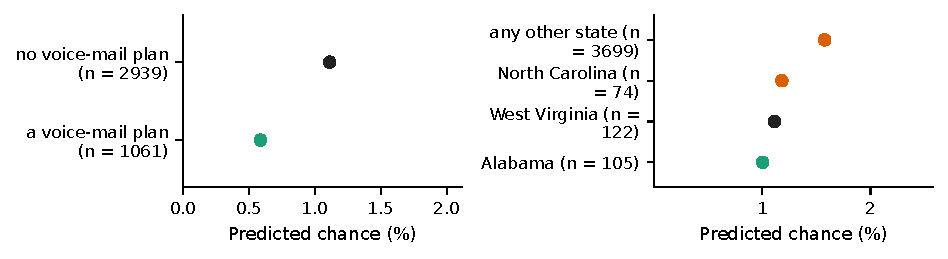
\includegraphics[width=\linewidth,height=0.88\textheight,keepaspectratio]{figures/churn100-s2-c1/ann_95-categories-small.pdf}
\caption{Voice-mail discount: The predicted value for the typical case at each level, through this part (n = training customers; grey: fewer than 20).}
\label{fig:churn100s2c1:plot-ann95-0}
\end{figure}
\begin{figure}[H]\centering
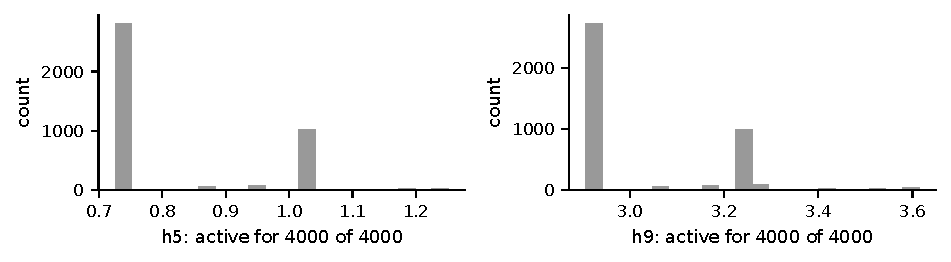
\includegraphics[width=\linewidth,height=0.88\textheight,keepaspectratio]{figures/churn100-s2-c1/ann_95-units.pdf}
\caption{Voice-mail discount: This part's hidden units: each unit's output against its main numeric input (top) and how often it is active (bottom).}
\label{fig:churn100s2c1:plot-ann95-1}
\end{figure}
\par\smallskip\noindent{\small Technical detail: \ref{tech:ann95}.\par}
\subsubsection{Heavy evening use}\label{rd:ann94}
\noindent{\footnotesize Part of: The whole model (\ref{rd:ann102}).\par}
\noindent{\small Figure~\ref{fig:churn100s2c1:parts-ann94} shows what feeds this part; Figure~\ref{fig:churn100s2c1:units-ann94} its units and every connection into them (dashed boxes: connections from or to other parts, drawn in their own sections).\par}
\begin{figure}[H]\centering
\resizebox{!}{\ifdim\height>0.5\textheight 0.5\textheight\else\height\fi}{%
\resizebox{\ifdim\width>\linewidth\linewidth\else\width\fi}{!}{%
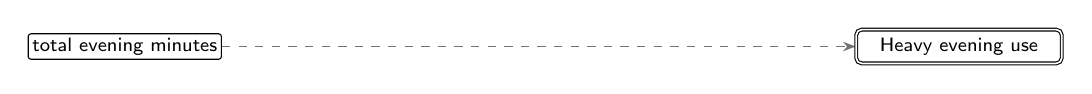
\begin{tikzpicture}[
  font=\sffamily\scriptsize, >={Stealth[length=1.6mm]},
  inp/.style={draw, rounded corners=1pt, fill=white, inner sep=1.5pt, minimum height=3.2mm, anchor=east},
  abox/.style={draw, thick, rounded corners=2pt, align=center, inner sep=3pt, minimum height=6mm, text width=42mm},
  outp/.style={draw, double, rounded corners=2pt, fill=white, align=center, inner sep=3pt, text width=24mm},
  agg/.style={draw=black!55},
]
\node[inp] (i0) at (0,-0.0) {total evening minutes};
\node[outp] (out) at (9.36,0) {Heavy evening use};
\begin{scope}[on background layer]
\draw[->, agg, thin, dashed] (i0.east) -- (out.west);
\end{scope}
\end{tikzpicture}}}%
\caption{Heavy evening use: what feeds it, one level down.}
\label{fig:churn100s2c1:parts-ann94}
\end{figure}
\begin{figure}[H]\centering
\resizebox{\ifdim\width>\linewidth\linewidth\else\width\fi}{!}{%
\definecolor{netup}{HTML}{D95F02}\definecolor{netdown}{HTML}{1B9E77}\definecolor{netmixed}{HTML}{7F7F7F}%
\begin{tikzpicture}[
  font=\sffamily\scriptsize, >={Stealth[length=1.4mm]},
  inp/.style={draw, circle, fill=white, minimum size=3.2mm, inner sep=0pt},
  hid/.style={draw, circle, fill=white, minimum size=5.2mm, inner sep=0.5pt, font=\sffamily\tiny},
  exitbox/.style={draw, thick, rectangle, fill=white, align=center, text width=17mm, minimum height=5mm, inner sep=1.5pt, font=\sffamily\tiny},
  sumbox/.style={draw, thick, dashed, rectangle, fill=white, align=center, text width=17mm, minimum height=5mm, inner sep=1.5pt, font=\sffamily\tiny},
  outp/.style={draw, thick, regular polygon, regular polygon sides=6, fill=white, minimum size=10mm, inner sep=0pt, font=\sffamily\tiny, align=center},
  stub/.style={draw, dashed, rounded corners=2pt, fill=white, align=center, inner sep=2pt, font=\sffamily\tiny, text width=15mm},
  inlab/.style={font=\sffamily\tiny, align=center, text width=15mm, inner sep=1pt, fill=white, fill opacity=0.8, text opacity=1},
  wpos/.style={draw=NavyBlue}, wneg/.style={draw=BrickRed}, wagg/.style={draw=black!45, line width=1.2pt},
  wmix/.style={draw=Plum},
]
\node[exitbox] (n476) at (1.7,1.9) {Heavy evening use $\downarrow$};
\node[inp, draw=netdown, very thick] (ninxxtotalxevexminutes) at (1.7,0.0) {};
\path (ninxxtotalxevexminutes.south) node[inlab, anchor=north] (labninxxtotalxevexminutes) {total evening minutes $\downarrow$};
\node[stub] (ntoxxthexmodelxoutput) at (1.7,3.45) {to the model output};
\begin{scope}[on background layer]
\node[fit=(n476) , inner sep=8pt, rounded corners=5pt, fill=Goldenrod!10, draw=Goldenrod!45] (clu0) {};
\draw[->, wpos, line width=0.63pt] (ninxxtotalxevexminutes) -- (n476);
\draw[->, wneg, line width=0.44pt] (n476) -- (ntoxxthexmodelxoutput);
\end{scope}
\node[font=\sffamily\scriptsize\bfseries, text=Goldenrod!55!black, anchor=south west, inner sep=1pt, fill=white, fill opacity=0.85, text opacity=1] at (clu0.north west) {Heavy evening use};
\end{tikzpicture}}%
\caption{Heavy evening use: its units and every connection into them. Blue: positive weight (raises the score); red: negative weight (lowers it); thicker: larger weight. Orange outline and up arrow: raises the final prediction; teal and down arrow: lowers it; grey and double arrow: depends.}
\label{fig:churn100s2c1:units-ann94}
\end{figure}
\paragraph{Hypothesis.} This part lowers the chance of leaving a little for customers with heavy evening use: evening minutes add nothing until about 239 minutes, then lower it steadily.\,{\scriptsize\textcolor{NavyBlue}{[C134]}}
\paragraph{Evidence.} It acts on 885 of 4000 training customers, 165 of whom left; for the typical customer it acts on, the chance is about 5\% without it and about 4\% with it.\,{\scriptsize\textcolor{NavyBlue}{[C136]}} Through it, evening minutes change nothing until about 239 minutes, then lower a typical customer's chance steadily, from about 1\% at 138 minutes to under 1\% at 266 minutes.\,{\scriptsize\textcolor{NavyBlue}{[C134]}} Its formula reproduces the part exactly on all 4000 training customers.\,{\scriptsize\textcolor{NavyBlue}{[C137]}}
\par\noindent{\small Evidence plots: Figure~\ref{fig:churn100s2c1:plot-ann94-0}, Figure~\ref{fig:churn100s2c1:plot-ann94-1}, Figure~\ref{fig:churn100s2c1:plot-ann94-2}.\par}
\par\noindent{\small Figure~\ref{fig:churn100s2c1:plot-ann94-1} shows this part's own output, unit h3: it switches on at about 238.8 minutes of total evening minutes, and is zero below.\par}
\begin{figure}[H]\centering
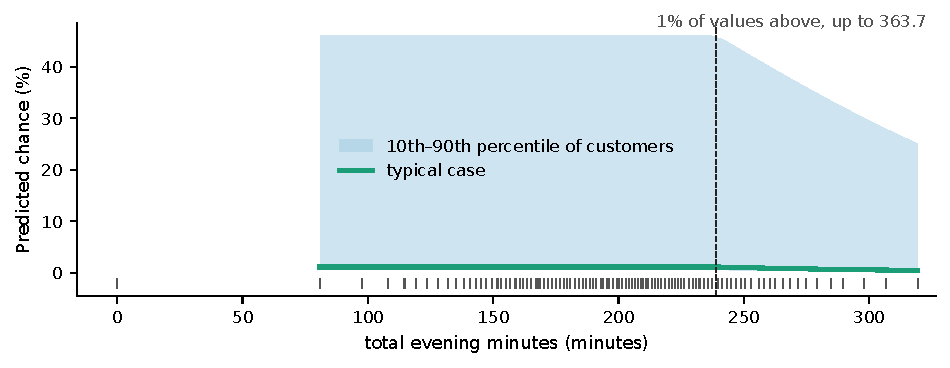
\includegraphics[width=\linewidth,height=0.88\textheight,keepaspectratio]{figures/churn100-s2-c1/ann_94-response.pdf}
\caption{Heavy evening use: Response curves through this part: the typical case (bold), the 10th to 90th percentile of individual customers (band), the fold or step point (dashed) with its spread across them (grey), and the observed values (ticks).}
\label{fig:churn100s2c1:plot-ann94-0}
\end{figure}
\begin{figure}[H]\centering
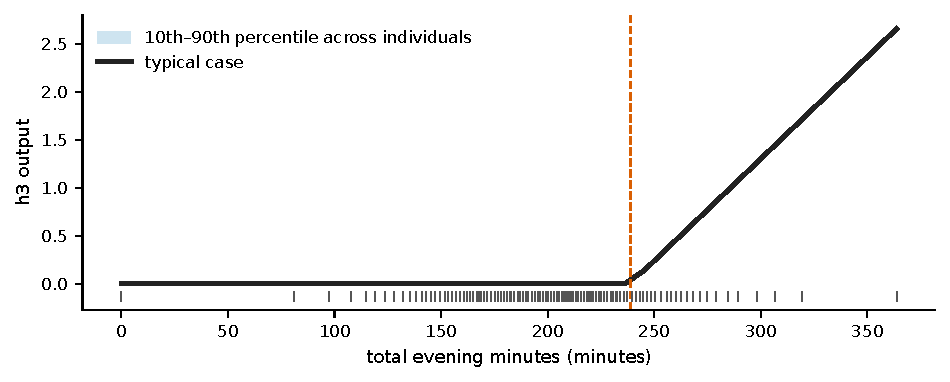
\includegraphics[width=\linewidth,height=0.88\textheight,keepaspectratio]{figures/churn100-s2-c1/ann_94-partial-476.pdf}
\caption{Heavy evening use: This part's own output, unit h3 (the output of 'Heavy evening use'), on its own scale (its activation), with every other input at the typical case; it is active for 885 of 4000. Bold: the typical case; band: 10th to 90th percentile across individuals; dashed: where it switches on; ticks: the data.}
\label{fig:churn100s2c1:plot-ann94-1}
\end{figure}
\begin{figure}[H]\centering
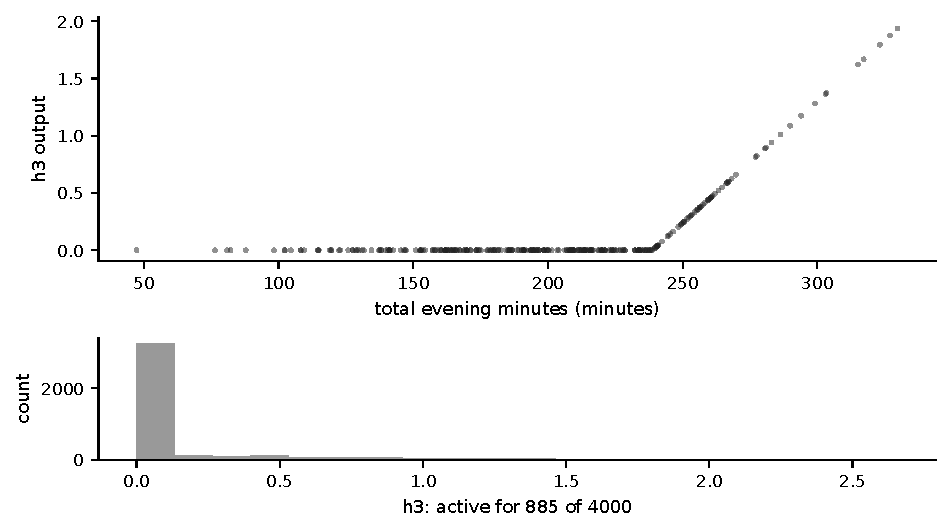
\includegraphics[width=\linewidth,height=0.88\textheight,keepaspectratio]{figures/churn100-s2-c1/ann_94-units.pdf}
\caption{Heavy evening use: This part's hidden units: each unit's output against its main numeric input (top) and how often it is active (bottom).}
\label{fig:churn100s2c1:plot-ann94-2}
\end{figure}
\par\smallskip\noindent{\small Technical detail: \ref{tech:ann94}.\par}
\subsubsection{State units}\label{rd:ann96}
\noindent{\footnotesize Part of: The whole model (\ref{rd:ann102}).\par}
\noindent{\small Figure~\ref{fig:churn100s2c1:parts-ann96} shows what feeds this part; Figure~\ref{fig:churn100s2c1:units-ann96} its units and every connection into them (dashed boxes: connections from or to other parts, drawn in their own sections).\par}
\begin{figure}[H]\centering
\resizebox{!}{\ifdim\height>0.5\textheight 0.5\textheight\else\height\fi}{%
\resizebox{\ifdim\width>\linewidth\linewidth\else\width\fi}{!}{%
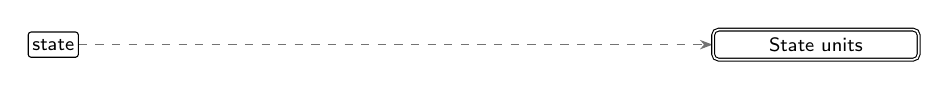
\begin{tikzpicture}[
  font=\sffamily\scriptsize, >={Stealth[length=1.6mm]},
  inp/.style={draw, rounded corners=1pt, fill=white, inner sep=1.5pt, minimum height=3.2mm, anchor=east},
  abox/.style={draw, thick, rounded corners=2pt, align=center, inner sep=3pt, minimum height=6mm, text width=42mm},
  outp/.style={draw, double, rounded corners=2pt, fill=white, align=center, inner sep=3pt, text width=24mm},
  agg/.style={draw=black!55},
]
\node[inp] (i0) at (0,-0.0) {state};
\node[outp] (out) at (9.36,0) {State units};
\begin{scope}[on background layer]
\draw[->, agg, thin, dashed] (i0.east) -- (out.west);
\end{scope}
\end{tikzpicture}}}%
\caption{State units: what feeds it, one level down.}
\label{fig:churn100s2c1:parts-ann96}
\end{figure}
\begin{figure}[H]\centering
\resizebox{\ifdim\width>\linewidth\linewidth\else\width\fi}{!}{%
\definecolor{netup}{HTML}{D95F02}\definecolor{netdown}{HTML}{1B9E77}\definecolor{netmixed}{HTML}{7F7F7F}%
\begin{tikzpicture}[
  font=\sffamily\scriptsize, >={Stealth[length=1.4mm]},
  inp/.style={draw, circle, fill=white, minimum size=3.2mm, inner sep=0pt},
  hid/.style={draw, circle, fill=white, minimum size=5.2mm, inner sep=0.5pt, font=\sffamily\tiny},
  exitbox/.style={draw, thick, rectangle, fill=white, align=center, text width=17mm, minimum height=5mm, inner sep=1.5pt, font=\sffamily\tiny},
  sumbox/.style={draw, thick, dashed, rectangle, fill=white, align=center, text width=17mm, minimum height=5mm, inner sep=1.5pt, font=\sffamily\tiny},
  outp/.style={draw, thick, regular polygon, regular polygon sides=6, fill=white, minimum size=10mm, inner sep=0pt, font=\sffamily\tiny, align=center},
  stub/.style={draw, dashed, rounded corners=2pt, fill=white, align=center, inner sep=2pt, font=\sffamily\tiny, text width=15mm},
  inlab/.style={font=\sffamily\tiny, align=center, text width=15mm, inner sep=1pt, fill=white, fill opacity=0.8, text opacity=1},
  wpos/.style={draw=NavyBlue}, wneg/.style={draw=BrickRed}, wagg/.style={draw=black!45, line width=1.2pt},
  wmix/.style={draw=Plum},
]
\node[hid] (n14942) at (3.35,1.9) {h19};
\node[hid] (n6730) at (3.35,3.25) {h11};
\node[hid] (n13827) at (3.35,4.6) {h18};
\node[hid] (n11951) at (1.85,1.9) {h16};
\node[hid] (n10249) at (0.35,1.9) {h14};
\node[hid] (n8896) at (6.35,1.9) {h13};
\node[hid] (n3861) at (4.85,1.9) {h8};
\node[inp, draw=netmixed, very thick] (ngrpxxstate) at (3.35,0.0) {};
\path (ngrpxxstate.south) node[inlab, anchor=north] (labngrpxxstate) {state (31 of 51 used) $\updownarrow$};
\node[stub] (ntoxxthexmodelxoutput) at (3.35,6.15) {to the model output};
\begin{scope}[on background layer]
\node[fit=(n14942) (n6730) (n13827) (n11951) (n10249) (n8896) (n3861) , inner sep=8pt, rounded corners=5pt, fill=Cerulean!10, draw=Cerulean!45] (clu0) {};
\draw[->, wneg, line width=0.25pt] (n11951) -- (n6730);
\draw[->, wpos, line width=0.60pt] (n6730) -- (n13827);
\draw[->, wneg, line width=0.30pt] (n3861) -- (ntoxxthexmodelxoutput);
\draw[->, wpos, line width=0.26pt] (n8896) -- (ntoxxthexmodelxoutput);
\draw[->, wpos, line width=0.26pt] (n10249) -- (ntoxxthexmodelxoutput);
\draw[->, wpos, line width=0.40pt] (n13827) -- (ntoxxthexmodelxoutput);
\draw[->, wpos, line width=0.26pt] (n14942) -- (ntoxxthexmodelxoutput);
\draw[->, wneg, line width=0.60pt] (ngrpxxstate) -- node[pos=0.8, sloped, above, font=\sffamily\tiny, inner sep=1pt, fill=white, fill opacity=0.8, text opacity=1] {-1.00} (n8896);
\draw[->, wmix, line width=0.40pt] (ngrpxxstate) -- node[pos=0.8, sloped, above, font=\sffamily\tiny, inner sep=1pt, fill=white, fill opacity=0.8, text opacity=1] {3 edges, -0.42 to +0.00} (n6730);
\draw[->, wneg, line width=0.52pt] (ngrpxxstate) -- node[pos=0.8, sloped, above, font=\sffamily\tiny, inner sep=1pt, fill=white, fill opacity=0.8, text opacity=1] {-0.77} (n3861);
\draw[->, wpos, line width=0.60pt] (ngrpxxstate) -- node[pos=0.8, sloped, above, font=\sffamily\tiny, inner sep=1pt, fill=white, fill opacity=0.8, text opacity=1] {+1.00} (n10249);
\draw[->, wpos, line width=0.60pt] (ngrpxxstate) -- node[pos=0.8, sloped, above, font=\sffamily\tiny, inner sep=1pt, fill=white, fill opacity=0.8, text opacity=1] {+1.00} (n11951);
\draw[->, wpos, line width=0.60pt] (ngrpxxstate) -- node[pos=0.8, sloped, above, font=\sffamily\tiny, inner sep=1pt, fill=white, fill opacity=0.8, text opacity=1] {+1.00} (n14942);
\end{scope}
\node[font=\sffamily\scriptsize\bfseries, text=Cerulean!55!black, anchor=south west, inner sep=1pt, fill=white, fill opacity=0.85, text opacity=1] at (clu0.north west) {State units};
\end{tikzpicture}}%
\caption{State units: its units and every connection into them. Blue: positive weight (raises the score); red: negative weight (lowers it); thicker: larger weight. Orange outline and up arrow: raises the final prediction; teal and down arrow: lowers it; grey and double arrow: depends.}
\label{fig:churn100s2c1:units-ann96}
\end{figure}
\paragraph{Hypothesis.} This part adds small state offsets: up in Arizona and Ohio, down in Nevada.\,{\scriptsize\textcolor{NavyBlue}{[C138, C139, C140]}}
\paragraph{Evidence.} Through it, a typical customer's chance moves by less than half a point: up in Arizona and Ohio, down in Nevada, with Missouri and Massachusetts almost unchanged.\,{\scriptsize\textcolor{NavyBlue}{[C138, C139, C140, C141, C142]}} Its formula reproduces the part exactly on all 4000 training customers.\,{\scriptsize\textcolor{NavyBlue}{[C143]}}
\par\noindent{\small Evidence plots: Figure~\ref{fig:churn100s2c1:plot-ann96-0}, Figure~\ref{fig:churn100s2c1:plot-ann96-1}.\par}
\begin{figure}[H]\centering
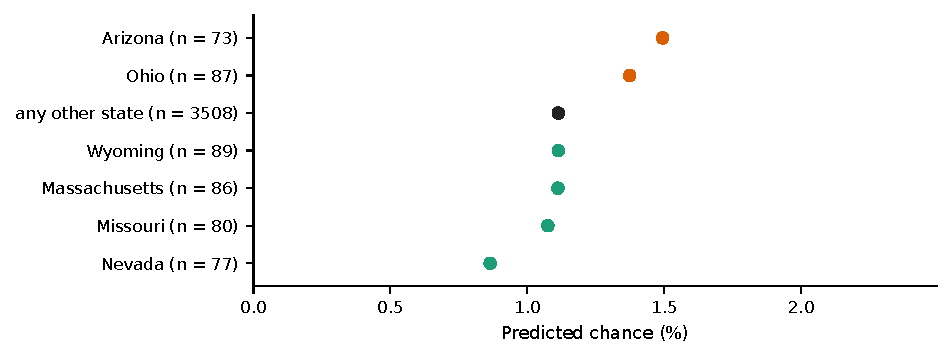
\includegraphics[width=\linewidth,height=0.88\textheight,keepaspectratio]{figures/churn100-s2-c1/ann_96-categories-C138.pdf}
\caption{State units: The predicted value for the typical case at each level, through this part (n = training customers; grey: fewer than 20).}
\label{fig:churn100s2c1:plot-ann96-0}
\end{figure}
\begin{figure}[H]\centering
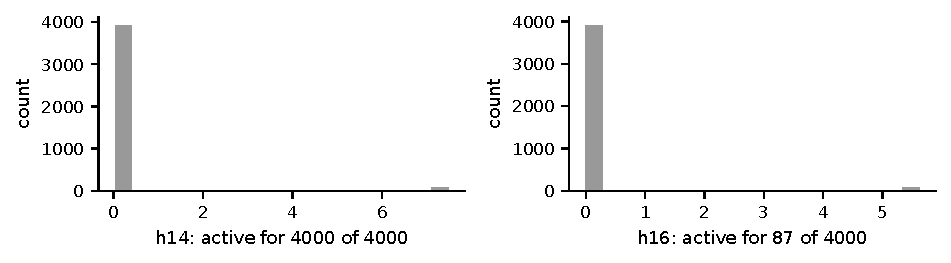
\includegraphics[width=\linewidth,height=0.88\textheight,keepaspectratio]{figures/churn100-s2-c1/ann_96-units.pdf}
\caption{State units: This part's hidden units: each unit's output against its main numeric input (top) and how often it is active (bottom).}
\label{fig:churn100s2c1:plot-ann96-1}
\end{figure}
\par\smallskip\noindent{\small Technical detail: \ref{tech:ann96}.\par}
\subsubsection{Daytime calls and Tennessee}\label{rd:ann97}
\noindent{\footnotesize Part of: The whole model (\ref{rd:ann102}).\par}
\noindent{\small Figure~\ref{fig:churn100s2c1:parts-ann97} shows what feeds this part; Figure~\ref{fig:churn100s2c1:units-ann97} its units and every connection into them (dashed boxes: connections from or to other parts, drawn in their own sections).\par}
\begin{figure}[H]\centering
\resizebox{!}{\ifdim\height>0.5\textheight 0.5\textheight\else\height\fi}{%
\resizebox{\ifdim\width>\linewidth\linewidth\else\width\fi}{!}{%
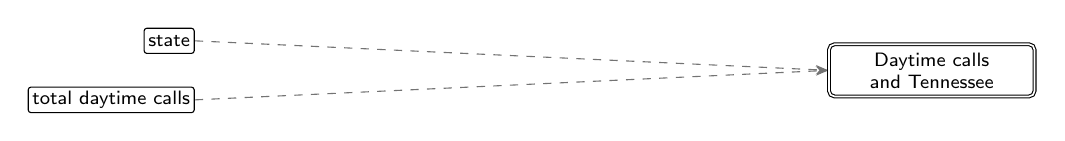
\begin{tikzpicture}[
  font=\sffamily\scriptsize, >={Stealth[length=1.6mm]},
  inp/.style={draw, rounded corners=1pt, fill=white, inner sep=1.5pt, minimum height=3.2mm, anchor=east},
  abox/.style={draw, thick, rounded corners=2pt, align=center, inner sep=3pt, minimum height=6mm, text width=42mm},
  outp/.style={draw, double, rounded corners=2pt, fill=white, align=center, inner sep=3pt, text width=24mm},
  agg/.style={draw=black!55},
]
\node[inp] (i0) at (0,0.375) {state};
\node[inp] (i1) at (0,-0.375) {total daytime calls};
\node[outp] (out) at (9.36,0) {Daytime calls and Tennessee};
\begin{scope}[on background layer]
\draw[->, agg, thin, dashed] (i0.east) -- (out.west);
\draw[->, agg, thin, dashed] (i1.east) -- (out.west);
\end{scope}
\end{tikzpicture}}}%
\caption{Daytime calls and Tennessee: what feeds it, one level down.}
\label{fig:churn100s2c1:parts-ann97}
\end{figure}
\begin{figure}[H]\centering
\resizebox{\ifdim\width>\linewidth\linewidth\else\width\fi}{!}{%
\definecolor{netup}{HTML}{D95F02}\definecolor{netdown}{HTML}{1B9E77}\definecolor{netmixed}{HTML}{7F7F7F}%
\begin{tikzpicture}[
  font=\sffamily\scriptsize, >={Stealth[length=1.4mm]},
  inp/.style={draw, circle, fill=white, minimum size=3.2mm, inner sep=0pt},
  hid/.style={draw, circle, fill=white, minimum size=5.2mm, inner sep=0.5pt, font=\sffamily\tiny},
  exitbox/.style={draw, thick, rectangle, fill=white, align=center, text width=17mm, minimum height=5mm, inner sep=1.5pt, font=\sffamily\tiny},
  sumbox/.style={draw, thick, dashed, rectangle, fill=white, align=center, text width=17mm, minimum height=5mm, inner sep=1.5pt, font=\sffamily\tiny},
  outp/.style={draw, thick, regular polygon, regular polygon sides=6, fill=white, minimum size=10mm, inner sep=0pt, font=\sffamily\tiny, align=center},
  stub/.style={draw, dashed, rounded corners=2pt, fill=white, align=center, inner sep=2pt, font=\sffamily\tiny, text width=15mm},
  inlab/.style={font=\sffamily\tiny, align=center, text width=15mm, inner sep=1pt, fill=white, fill opacity=0.8, text opacity=1},
  wpos/.style={draw=NavyBlue}, wneg/.style={draw=BrickRed}, wagg/.style={draw=black!45, line width=1.2pt},
  wmix/.style={draw=Plum},
]
\node[exitbox] (n11427) at (2.7,1.9) {Daytime calls and Tennessee $\uparrow$};
\node[inp, draw=netmixed, very thick] (ngrpxxstate) at (1.8,0.0) {};
\path (ngrpxxstate.south) node[inlab, anchor=north] (labngrpxxstate) {state (31 of 51 used) $\updownarrow$};
\node[inp, draw=netdown, very thick] (ninxxtotalxdayxcalls) at (3.6,0.0) {};
\path (ninxxtotalxdayxcalls.south) node[inlab, anchor=north] (labninxxtotalxdayxcalls) {total daytime calls $\downarrow$};
\node[stub] (ntoxxthexmodelxoutput) at (2.7,3.45) {to the model output};
\begin{scope}[on background layer]
\node[fit=(n11427) , inner sep=8pt, rounded corners=5pt, fill=Mahogany!10, draw=Mahogany!45] (clu0) {};
\draw[->, wneg, line width=0.29pt] (ninxxtotalxdayxcalls) -- (n11427);
\draw[->, wpos, line width=0.27pt] (n11427) -- (ntoxxthexmodelxoutput);
\draw[->, wpos, line width=0.60pt] (ngrpxxstate) -- node[pos=0.8, sloped, above, font=\sffamily\tiny, inner sep=1pt, fill=white, fill opacity=0.8, text opacity=1] {+1.00} (n11427);
\end{scope}
\node[font=\sffamily\scriptsize\bfseries, text=Mahogany!55!black, anchor=south west, inner sep=1pt, fill=white, fill opacity=0.85, text opacity=1] at (clu0.north west) {Daytime calls and Tennessee};
\end{tikzpicture}}%
\caption{Daytime calls and Tennessee: its units and every connection into them. Blue: positive weight (raises the score); red: negative weight (lowers it); thicker: larger weight. Orange outline and up arrow: raises the final prediction; teal and down arrow: lowers it; grey and double arrow: depends.}
\label{fig:churn100s2c1:units-ann97}
\end{figure}
\paragraph{Hypothesis.} This part gives customers in Tennessee a small rise in the chance of leaving; daytime calls barely change it.\,{\scriptsize\textcolor{NavyBlue}{[C144, C145]}}
\paragraph{Evidence.} Through it, being in Tennessee takes a typical customer's chance from about 1\% to about 2\%, and going from 75 to 125 daytime calls barely changes it.\,{\scriptsize\textcolor{NavyBlue}{[C144, C145]}} Its formula reproduces the part exactly on all 4000 training customers.\,{\scriptsize\textcolor{NavyBlue}{[C149]}}
\par\noindent{\small Evidence plots: Figure~\ref{fig:churn100s2c1:plot-ann97-0}, Figure~\ref{fig:churn100s2c1:plot-ann97-1}, Figure~\ref{fig:churn100s2c1:plot-ann97-2}, Figure~\ref{fig:churn100s2c1:plot-ann97-3}.\par}
\par\noindent{\small Figure~\ref{fig:churn100s2c1:plot-ann97-2} shows this part's own output, unit h15: it switches on at about 113 calls of total daytime calls, and is zero below.\par}
\begin{figure}[H]\centering
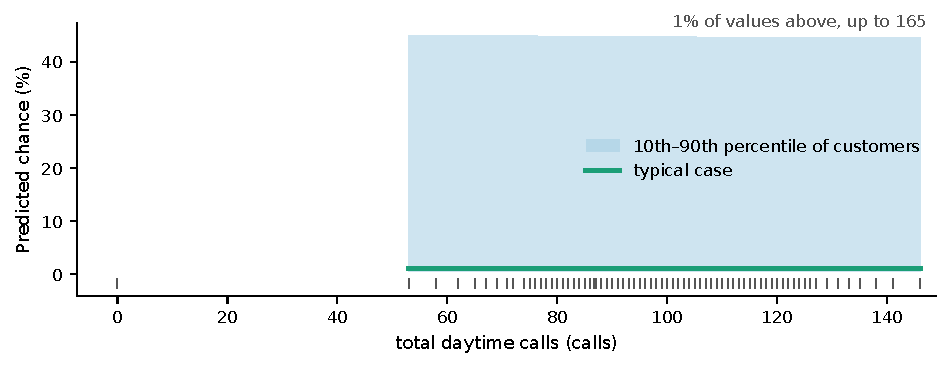
\includegraphics[width=\linewidth,height=0.88\textheight,keepaspectratio]{figures/churn100-s2-c1/ann_97-response.pdf}
\caption{Daytime calls and Tennessee: Response curves through this part: the typical case (bold), the 10th to 90th percentile of individual customers (band), the fold or step point (dashed) with its spread across them (grey), and the observed values (ticks).}
\label{fig:churn100s2c1:plot-ann97-0}
\end{figure}
\begin{figure}[H]\centering
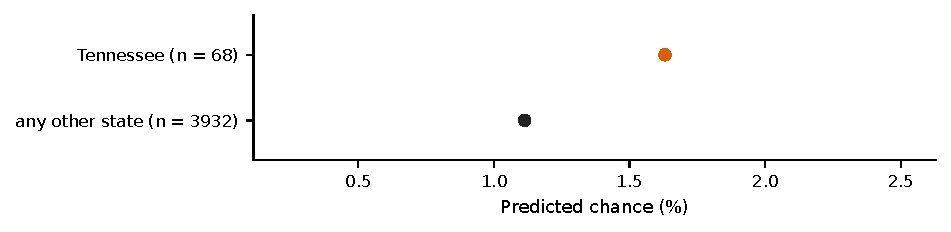
\includegraphics[width=\linewidth,height=0.88\textheight,keepaspectratio]{figures/churn100-s2-c1/ann_97-categories-small.pdf}
\caption{Daytime calls and Tennessee: The predicted value for the typical case at each level, through this part (n = training customers; grey: fewer than 20).}
\label{fig:churn100s2c1:plot-ann97-1}
\end{figure}
\begin{figure}[H]\centering
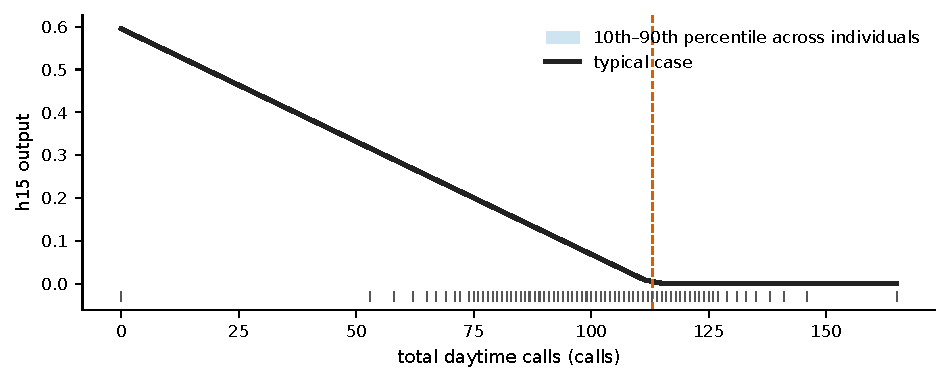
\includegraphics[width=\linewidth,height=0.88\textheight,keepaspectratio]{figures/churn100-s2-c1/ann_97-partial-11427.pdf}
\caption{Daytime calls and Tennessee: This part's own output, unit h15 (the output of 'Daytime calls and Tennessee'), on its own scale (its activation), with every other input at the typical case; it is active for 2994 of 4000. Bold: the typical case; band: 10th to 90th percentile across individuals; dashed: where it switches on; ticks: the data.}
\label{fig:churn100s2c1:plot-ann97-2}
\end{figure}
\begin{figure}[H]\centering
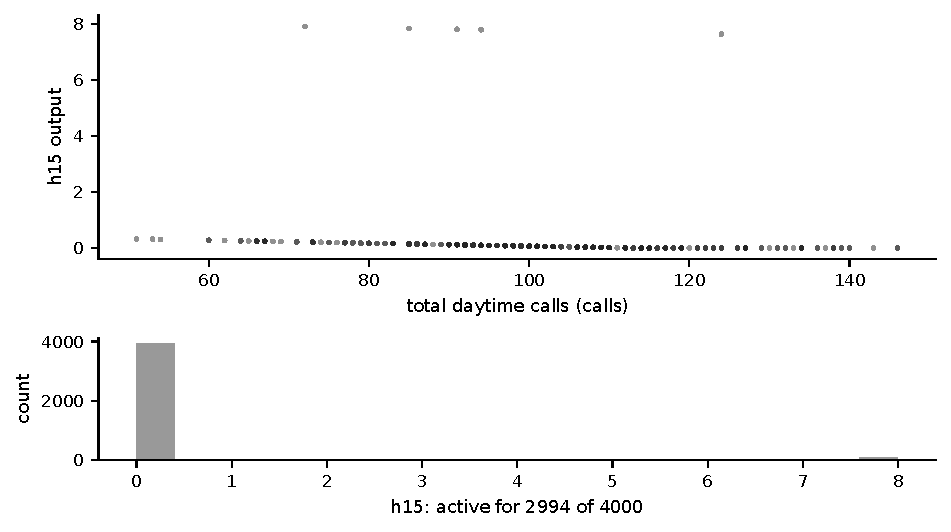
\includegraphics[width=\linewidth,height=0.88\textheight,keepaspectratio]{figures/churn100-s2-c1/ann_97-units.pdf}
\caption{Daytime calls and Tennessee: This part's hidden units: each unit's output against its main numeric input (top) and how often it is active (bottom).}
\label{fig:churn100s2c1:plot-ann97-3}
\end{figure}
\par\smallskip\noindent{\small Technical detail: \ref{tech:ann97}.\par}
\subsubsection{Small state unit}\label{rd:ann92}
\noindent{\footnotesize Part of: The whole model (\ref{rd:ann102}).\par}
\noindent{\small Figure~\ref{fig:churn100s2c1:parts-ann92} shows what feeds this part; Figure~\ref{fig:churn100s2c1:units-ann92} its units and every connection into them (dashed boxes: connections from or to other parts, drawn in their own sections).\par}
\begin{figure}[H]\centering
\resizebox{!}{\ifdim\height>0.5\textheight 0.5\textheight\else\height\fi}{%
\resizebox{\ifdim\width>\linewidth\linewidth\else\width\fi}{!}{%
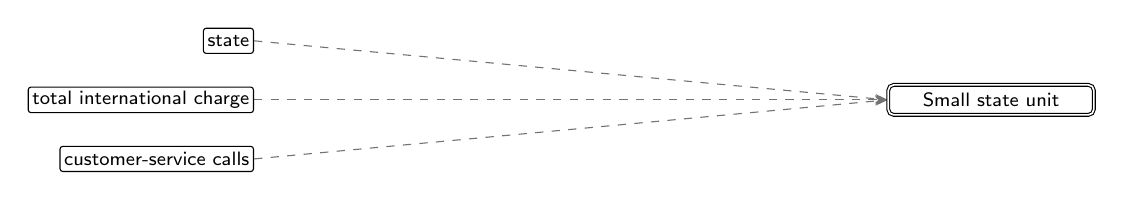
\begin{tikzpicture}[
  font=\sffamily\scriptsize, >={Stealth[length=1.6mm]},
  inp/.style={draw, rounded corners=1pt, fill=white, inner sep=1.5pt, minimum height=3.2mm, anchor=east},
  abox/.style={draw, thick, rounded corners=2pt, align=center, inner sep=3pt, minimum height=6mm, text width=42mm},
  outp/.style={draw, double, rounded corners=2pt, fill=white, align=center, inner sep=3pt, text width=24mm},
  agg/.style={draw=black!55},
]
\node[inp] (i0) at (0,0.75) {state};
\node[inp] (i1) at (0,-0.0) {total international charge};
\node[inp] (i2) at (0,-0.75) {customer-service calls};
\node[outp] (out) at (9.36,0) {Small state unit};
\begin{scope}[on background layer]
\draw[->, agg, thin, dashed] (i0.east) -- (out.west);
\draw[->, agg, thin, dashed] (i1.east) -- (out.west);
\draw[->, agg, thin, dashed] (i2.east) -- (out.west);
\end{scope}
\end{tikzpicture}}}%
\caption{Small state unit: what feeds it, one level down.}
\label{fig:churn100s2c1:parts-ann92}
\end{figure}
\begin{figure}[H]\centering
\resizebox{\ifdim\width>\linewidth\linewidth\else\width\fi}{!}{%
\definecolor{netup}{HTML}{D95F02}\definecolor{netdown}{HTML}{1B9E77}\definecolor{netmixed}{HTML}{7F7F7F}%
\begin{tikzpicture}[
  font=\sffamily\scriptsize, >={Stealth[length=1.4mm]},
  inp/.style={draw, circle, fill=white, minimum size=3.2mm, inner sep=0pt},
  hid/.style={draw, circle, fill=white, minimum size=5.2mm, inner sep=0.5pt, font=\sffamily\tiny},
  exitbox/.style={draw, thick, rectangle, fill=white, align=center, text width=17mm, minimum height=5mm, inner sep=1.5pt, font=\sffamily\tiny},
  sumbox/.style={draw, thick, dashed, rectangle, fill=white, align=center, text width=17mm, minimum height=5mm, inner sep=1.5pt, font=\sffamily\tiny},
  outp/.style={draw, thick, regular polygon, regular polygon sides=6, fill=white, minimum size=10mm, inner sep=0pt, font=\sffamily\tiny, align=center},
  stub/.style={draw, dashed, rounded corners=2pt, fill=white, align=center, inner sep=2pt, font=\sffamily\tiny, text width=15mm},
  inlab/.style={font=\sffamily\tiny, align=center, text width=15mm, inner sep=1pt, fill=white, fill opacity=0.8, text opacity=1},
  wpos/.style={draw=NavyBlue}, wneg/.style={draw=BrickRed}, wagg/.style={draw=black!45, line width=1.2pt},
  wmix/.style={draw=Plum},
]
\node[hid] (n2627xa) at (2.7,3.25) {h21};
\node[hid] (n161) at (1.95,1.9) {h1};
\node[hid] (n9555xa) at (3.45,1.9) {h23};
\node[exitbox] (n252) at (2.7,4.6) {Small state unit $\uparrow$};
\node[inp, draw=netmixed, very thick] (ngrpxxstate) at (0.9,0.0) {};
\path (ngrpxxstate.south) node[inlab, anchor=north] (labngrpxxstate) {state (31 of 51 used) $\updownarrow$};
\node[inp, draw=netdown, very thick] (ninxxtotalxintlxcharge) at (2.7,0.0) {};
\path (ninxxtotalxintlxcharge.south) node[inlab, anchor=north] (labninxxtotalxintlxcharge) {total international charge $\downarrow$};
\node[inp, draw=netdown, very thick] (ninxxnumberxcustomerxservicexcalls) at (4.5,0.0) {};
\path (ninxxnumberxcustomerxservicexcalls.south) node[inlab, anchor=north] (labninxxnumberxcustomerxservicexcalls) {customer-service calls $\downarrow$};
\node[stub] (ntoxxthexmodelxoutput) at (2.7,6.15) {to the model output};
\begin{scope}[on background layer]
\node[fit=(n2627xa) (n161) (n9555xa) (n252) , inner sep=8pt, rounded corners=5pt, fill=OliveGreen!10, draw=OliveGreen!45] (clu0) {};
\draw[->, wpos, line width=0.53pt] (n161) -- (n252);
\draw[->, wneg, line width=0.38pt] (n2627xa) -- (n252);
\draw[->, wpos, line width=0.36pt] (n9555xa) -- (n2627xa);
\draw[->, wneg, line width=0.55pt] (ninxxtotalxintlxcharge) -- (n252);
\draw[->, wpos, line width=0.35pt] (ninxxnumberxcustomerxservicexcalls) -- (n2627xa);
\draw[->, wpos, line width=0.55pt] (ninxxnumberxcustomerxservicexcalls) -- (n9555xa);
\draw[->, wpos, line width=0.26pt] (n252) -- (ntoxxthexmodelxoutput);
\draw[->, wneg, line width=0.25pt] (ngrpxxstate) -- node[pos=0.8, sloped, above, font=\sffamily\tiny, inner sep=1pt, fill=white, fill opacity=0.8, text opacity=1] {-0.01} (n161);
\draw[->, wpos, line width=0.52pt] (ngrpxxstate) -- node[pos=0.8, sloped, above, font=\sffamily\tiny, inner sep=1pt, fill=white, fill opacity=0.8, text opacity=1] {2 edges, +0.44 to +0.76} (n252);
\end{scope}
\node[font=\sffamily\scriptsize\bfseries, text=OliveGreen!55!black, anchor=south west, inner sep=1pt, fill=white, fill opacity=0.85, text opacity=1] at (clu0.north west) {Small state unit};
\end{tikzpicture}}%
\caption{Small state unit: its units and every connection into them. Blue: positive weight (raises the score); red: negative weight (lowers it); thicker: larger weight. Orange outline and up arrow: raises the final prediction; teal and down arrow: lowers it; grey and double arrow: depends.}
\label{fig:churn100s2c1:units-ann92}
\end{figure}
\paragraph{Hypothesis.} This small part barely changes the chance of leaving: it adds less than a tenth of a point in Arkansas and Utah.\,{\scriptsize\textcolor{NavyBlue}{[C150, C153]}}
\paragraph{Evidence.} Through it, the chance moves by less than a tenth of a point in Arkansas and Utah, a higher international charge lowers it steadily by even less, and customer-service calls barely move it.\,{\scriptsize\textcolor{NavyBlue}{[C150, C153, C151, C152]}} Its formula reproduces the part exactly on all 4000 training customers.\,{\scriptsize\textcolor{NavyBlue}{[C161]}}
\par\noindent{\small Evidence plots: Figure~\ref{fig:churn100s2c1:plot-ann92-0}, Figure~\ref{fig:churn100s2c1:plot-ann92-1}, Figure~\ref{fig:churn100s2c1:plot-ann92-2}, Figure~\ref{fig:churn100s2c1:plot-ann92-3}, Figure~\ref{fig:churn100s2c1:plot-ann92-4}, Figure~\ref{fig:churn100s2c1:plot-ann92-5}.\par}
\par\medskip\noindent\textbf{Worked example: reading this part.} Figure~\ref{fig:churn100s2c1:plot-ann92-2} maps the part's own output over its main inputs. In the grey region it is switched off and adds nothing; past the black line it switches on, and the colour shows how much it adds to the score. The line is the rule in the claim (C164): it switches on when total international charge plus about 0.07 $\times$ customer-service calls below about 0.50 (for customer-service calls from about 0.00 to 1.73); total international charge plus about 0.14 $\times$ customer-service calls below about 0.62 (for customer-service calls from about 1.73 to 6.04). 153 of 4000 training customers lie on the 'on' side, and 12\% of them left, against 14\% of the others: the 'on' side holds mostly hollow points, so the part picks out low-risk cases. Figure~\ref{fig:churn100s2c1:plot-ann92-3} cuts the map into slices: the hinge moves as the other input changes, which is what a tilted line means. Figure~\ref{fig:churn100s2c1:plot-ann92-4} shows what this does to the final prediction for the typical case.\par
\begin{figure}[H]\centering
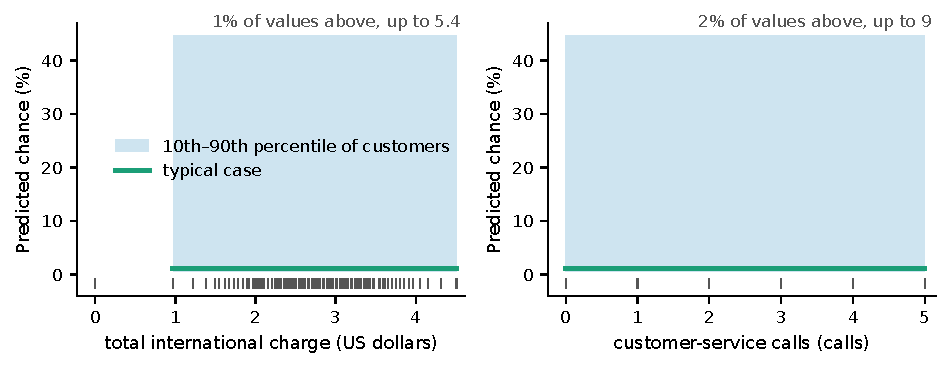
\includegraphics[width=\linewidth,height=0.88\textheight,keepaspectratio]{figures/churn100-s2-c1/ann_92-response.pdf}
\caption{Small state unit: Response curves through this part: the typical case (bold), the 10th to 90th percentile of individual customers (band), the fold or step point (dashed) with its spread across them (grey), and the observed values (ticks).}
\label{fig:churn100s2c1:plot-ann92-0}
\end{figure}
\begin{figure}[H]\centering
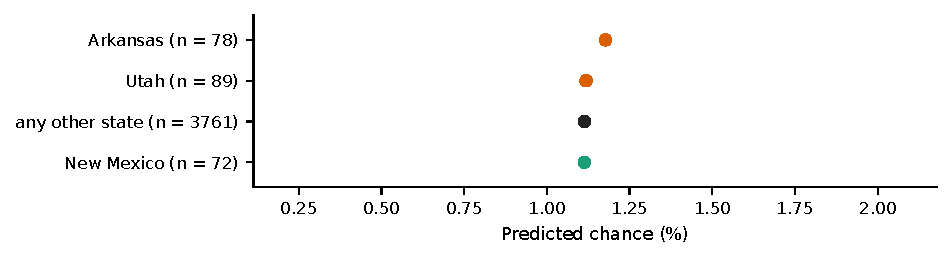
\includegraphics[width=\linewidth,height=0.88\textheight,keepaspectratio]{figures/churn100-s2-c1/ann_92-categories-small.pdf}
\caption{Small state unit: The predicted value for the typical case at each level, through this part (n = training customers; grey: fewer than 20).}
\label{fig:churn100s2c1:plot-ann92-1}
\end{figure}
\begin{figure}[H]\centering
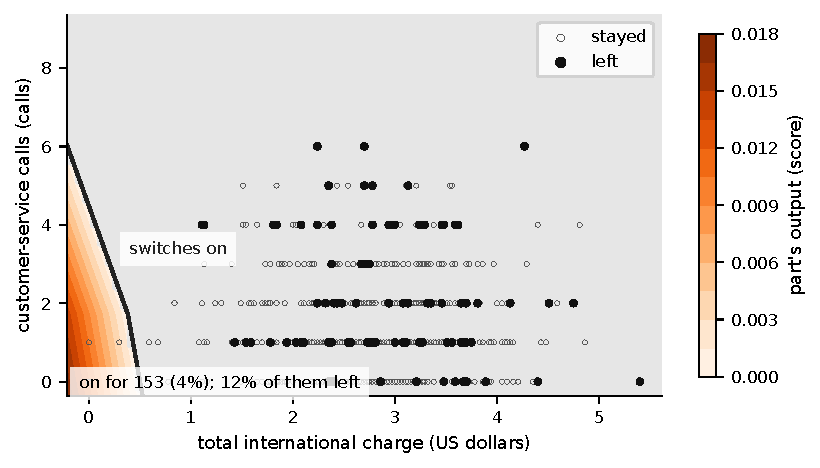
\includegraphics[width=\linewidth,height=0.88\textheight,keepaspectratio]{figures/churn100-s2-c1/ann_92-deep-map.pdf}
\caption{Small state unit: The part's own output over its two numeric inputs, other inputs at the typical case: colour where it is on, flat grey where it is switched off, the black line where it switches on; training customers as hollow (no event) and filled (event) points, so the part can be seen catching the events (the predicted-chance overlay was harder to read).}
\label{fig:churn100s2c1:plot-ann92-2}
\end{figure}
\begin{figure}[H]\centering
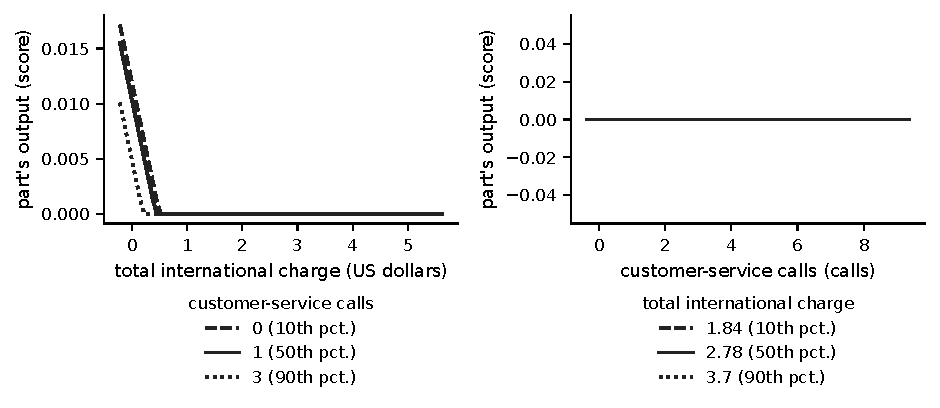
\includegraphics[width=\linewidth,height=0.88\textheight,keepaspectratio]{figures/churn100-s2-c1/ann_92-deep-slices.pdf}
\caption{Small state unit: Slices of the same map: the part's own output against each input at three values of the other, so the tilted boundary shows as a shifting hinge.}
\label{fig:churn100s2c1:plot-ann92-3}
\end{figure}
\begin{figure}[H]\centering
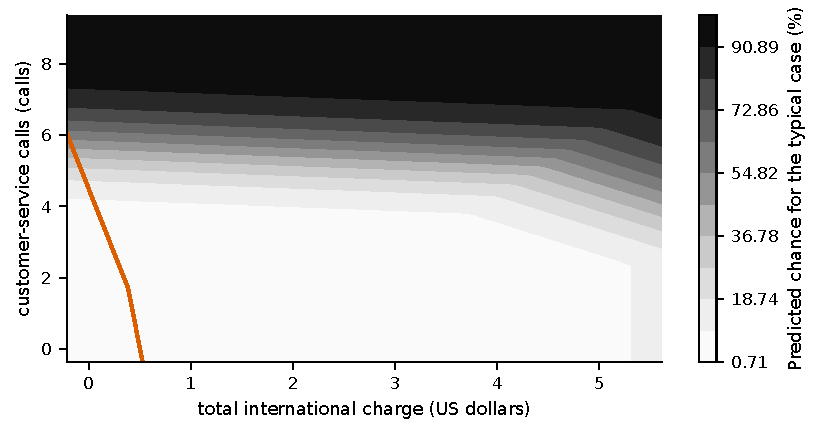
\includegraphics[width=\linewidth,height=0.88\textheight,keepaspectratio]{figures/churn100-s2-c1/ann_92-deep-risk.pdf}
\caption{Small state unit: The same map on the final scale: the predicted value for the typical case, with the switch-on line (orange).}
\label{fig:churn100s2c1:plot-ann92-4}
\end{figure}
\begin{figure}[H]\centering
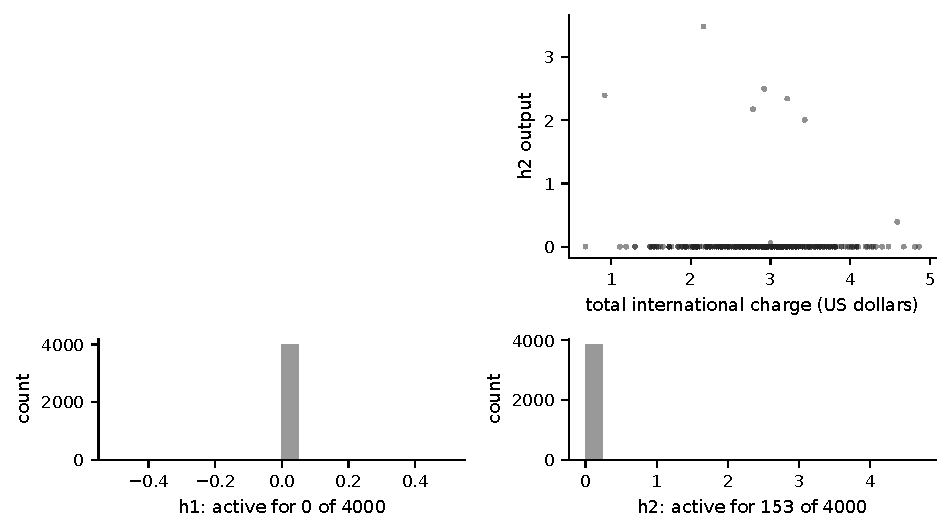
\includegraphics[width=\linewidth,height=0.88\textheight,keepaspectratio]{figures/churn100-s2-c1/ann_92-units.pdf}
\caption{Small state unit: This part's hidden units: each unit's output against its main numeric input (top) and how often it is active (bottom).}
\label{fig:churn100s2c1:plot-ann92-5}
\end{figure}
\par\smallskip\noindent{\small Technical detail: \ref{tech:ann92}.\par}
\subsection{Not supported by the model}
\begin{itemize}\setlength\itemsep{0pt}\small
\item C002: direction claim about total daytime minutes in the whole model: not supported by the model (17\% of patients have the opposite sign (allowed: 10\%)).
\item C017: direction claim about total evening charge in the whole model: not supported by the model (52\% of patients have the opposite sign (allowed: 10\%)).
\item C041: direction claim about state in the whole model: not supported by the model (45\% of patients have the opposite sign (allowed: 10\%)).
\item C044: direction claim about state in the whole model: not supported by the model (92\% of patients have the opposite sign (allowed: 10\%)).
\item C146: interaction claim about total daytime calls and state in part ann\_\allowbreak{}97: not supported by the model (the group difference is below 0.1 log-odds).
\item C147: threshold claim about total daytime calls in part ann\_\allowbreak{}97: not supported by the model (the fold changes the curve by only 0.014 log-odds compared with a straight line (needed 0.1); the effect past the fold is too small or not consistent across patients).
\item C148: subgroup claim about state and total daytime calls in part ann\_\allowbreak{}97: not supported by the model (its effect is negligible).
\item C154: interaction claim about number of calls to customer service and state in part ann\_\allowbreak{}92: not supported by the model (the part's own counterfactual difference has the opposite sign).
\item C155: interaction claim about total international charge and state in part ann\_\allowbreak{}92: not supported by the model (the group difference is below 0.1 log-odds).
\item C156: interaction claim about number of calls to customer service and total international charge in part ann\_\allowbreak{}92: not supported by the model (the group difference is below 0.1 log-odds; the part's own counterfactual difference has the opposite sign).
\item C157: threshold claim about number of calls to customer service in part ann\_\allowbreak{}92: not supported by the model (the fold changes the curve by only 0.015 log-odds compared with a straight line (needed 0.1); the effect past the fold is too small or not consistent across patients).
\item C158: threshold claim about total international charge in part ann\_\allowbreak{}92: not supported by the model (the effect past the fold is too small or not consistent across patients).
\item C159: subgroup claim about state and total international charge in part ann\_\allowbreak{}92: not supported by the model (its effect is negligible).
\item C160: null claim about state and total international charge in part ann\_\allowbreak{}92: not supported by the model (predictions move by up to 0.020).
\item C162: boundary claim about total daytime minutes and number of calls to customer service in part ann\_\allowbreak{}101: not supported by the model (no switch-on line could be traced on the first map to check against the data; no switch-on boundary in the observed range).
\item C163: boundary claim about total daytime minutes and number of calls to customer service in part ann\_\allowbreak{}91: not supported by the model (no switch-on line could be traced on the first map to check against the data; no switch-on boundary in the observed range).
\end{itemize}
\clearpage\section*{Technical detail: churn100-s2-c1}
\addcontentsline{toc}{section}{Technical detail: churn100-s2-c1}
\noindent{\small The record behind each part: the original hypothesis, the closed form, and every claim with its estimate (log-odds and odds ratio), range across patients, n and test check.\par}
\renewcommand{\thesubsection}{T.\arabic{subsection}}\setcounter{subsection}{0}
\subsection{The whole model}\label{tech:ann102}
\noindent{\footnotesize Annotation ann\_\allowbreak{}102 (churn\_\allowbreak{}logit). Reads: state, account length, area code, international calling plan, voice-mail plan, number of voice-mail messages, total daytime minutes, total daytime calls, total daytime charge, total evening minutes, total evening calls, total evening charge, total night-time minutes, total night-time calls, total night-time charge, total international minutes, total international calls, total international charge, number of calls to customer service.\par}
\paragraph{Original hypothesis (unchanged).} Root: logit P(churn) = -1.05 + linear\_\allowbreak{}backbone + service\_\allowbreak{}call\_\allowbreak{}nonlinear (identity\_\allowbreak{}svc = 1.60*807 + 1.81*1264 + 1.48*7208) - 0.95*1133 - 0.99*4051 (voicemail\_\allowbreak{}chain) - 0.55*476 (eve\_\allowbreak{}minutes\_\allowbreak{}hinge) + state\_\allowbreak{}offsets + 0.02*252 + 0.05*11427, purely additive in the logit; the sigmoid is the only coupling. 24 inputs are unconnected (total intl calls, night charge, evening calls, day charge and 20 state indicators) and have zero effect. Train AUC 0.901, accuracy 0.901. Performance sources (train): all children replaced by least-squares linear fits gives AUC 0.837 (an L2 logistic regression refit on all 71 inputs gets 0.843); restoring csc\_\allowbreak{}usage\_\allowbreak{}gate alone gives 0.898, csc\_\allowbreak{}hinge alone 0.851, eve\_\allowbreak{}minutes\_\allowbreak{}hinge alone 0.834, the others 0.837 (exactly or nearly linear). So the gain over linear comes from the service-call x low-usage gate. Rare-category switches: state:11/46/5 offsets of -2.24/-1.89/-1.46 logit on 73-80 customers (empirical -1.35/-0.91/-0.51); state:4 +1.35 (41 rows, empirical +0.80); state:47 +1.16 (72 rows, +0.92); state:49 -0.42 offset, down to -2.87 for 12 customers with 4+ calls (turns off the 4+-calls hinge); state:35 +0.40 (empirical +0.06).
\paragraph{Closed form.} Read through its parts (their formulas are in their own sections).
\paragraph{Split inputs.} To annotate the parts, the explanation split these inputs into copies (a refactoring step that does not change what the model computes); the diagrams draw each input once: customer-service calls (3 copies); total daytime calls (2 copies); total daytime minutes (2 copies); total evening charge (2 copies); total evening minutes (2 copies); total international charge (3 copies); a voice-mail plan (2 copies).
\paragraph{State: every level the model reads.} Whole-model change in the predicted chance for a typical customer when only the state changes from the reference; n = training customers in that level.\par\smallskip
{\scriptsize\rowcolors{2}{black!6}{white}
\begin{longtable}{@{}lllrlc@{}}
\toprule\rowcolor{white}
Claim & From & To & n & Chance & OK \\
\midrule\endhead
\bottomrule\endfoot
C003 & West Virginia & California & 41 & 1\% to 6\% & \textcolor{OliveGreen}{yes} \\
C004 & West Virginia & Washington & 72 & 1\% to 5\% & \textcolor{OliveGreen}{yes} \\
C006 & West Virginia & Montana & 75 & 1\% to 3\% & \textcolor{OliveGreen}{yes} \\
C007 & West Virginia & Maryland & 82 & 1\% to 3\% & \textcolor{OliveGreen}{yes} \\
C009 & West Virginia & Ohio & 87 & 1\% to 2\% & \textcolor{OliveGreen}{yes} \\
C010 & West Virginia & Tennessee & 68 & 1\% to 2\% & \textcolor{OliveGreen}{yes} \\
C013 & West Virginia & Connecticut & 80 & 1\% to 2\% & \textcolor{OliveGreen}{yes} \\
C015 & West Virginia & Oregon & 84 & 1\% to 2\% & \textcolor{OliveGreen}{yes} \\
C020 & West Virginia & Arizona & 73 & 1\% to 2\% & \textcolor{OliveGreen}{yes} \\
C022 & West Virginia & Utah & 89 & 1\% to 2\% & \textcolor{OliveGreen}{yes} \\
C023 & West Virginia & New Mexico & 72 & 1\% to 2\% & \textcolor{OliveGreen}{yes} \\
C024 & West Virginia & state other than Alaska, Alabama, Hawaii, Massachusetts, ... & 1587 & 1\% to 2\% & \textcolor{OliveGreen}{yes} \\
C025 & West Virginia & Massachusetts & 86 & 1\% to 2\% & \textcolor{OliveGreen}{yes} \\
C026 & West Virginia & Arkansas & 78 & 1\% to 2\% & \textcolor{OliveGreen}{yes} \\
C027 & West Virginia & North Carolina & 74 & 1\% to 2\% & \textcolor{OliveGreen}{yes} \\
C028 & West Virginia & North Dakota & 68 & 1\% to 2\% & \textcolor{OliveGreen}{yes} \\
C032 & West Virginia & Oklahoma & 79 & 1\% to 1\% & \textcolor{OliveGreen}{yes} \\
C037 & West Virginia & Nevada & 77 & 1\% to 1\% & \textcolor{OliveGreen}{yes} \\
C041 & West Virginia & South Dakota & 66 & 1\% to 1\% & \textcolor{BrickRed}{no} \\
C042 & West Virginia & New Hampshire & 74 & 1\% to 1\% & \textcolor{OliveGreen}{yes} \\
C045 & West Virginia & Nebraska & 72 & 1\% to 1\% & \textcolor{OliveGreen}{yes} \\
C044 & West Virginia & Alabama & 105 & 1\% to 1\% & \textcolor{BrickRed}{no} \\
C039 & West Virginia & Missouri & 80 & 1\% to 1\% & \textcolor{OliveGreen}{yes} \\
C036 & West Virginia & Wisconsin & 86 & 1\% to 1\% & \textcolor{OliveGreen}{yes} \\
C035 & West Virginia & Wyoming & 89 & 1\% to 1\% & \textcolor{OliveGreen}{yes} \\
C034 & West Virginia & Virginia & 91 & 1\% to 1\% & \textcolor{OliveGreen}{yes} \\
C030 & West Virginia & Alaska & 56 & 1\% to 1\% & \textcolor{OliveGreen}{yes} \\
C029 & West Virginia & Pennsylvania & 56 & 1\% to 1\% & \textcolor{OliveGreen}{yes} \\
C021 & West Virginia & Colorado & 78 & 1\% to $<$1\% & \textcolor{OliveGreen}{yes} \\
C019 & West Virginia & Vermont & 80 & 1\% to $<$1\% & \textcolor{OliveGreen}{yes} \\
C016 & West Virginia & Hawaii & 73 & 1\% to $<$1\% & \textcolor{OliveGreen}{yes} \\
\end{longtable}}
\paragraph{Evidence table} (next page, landscape).
\begin{landscape}
{\scriptsize\setlength{\tabcolsep}{3pt}\renewcommand{\arraystretch}{1.15}
\rowcolors{2}{black!6}{white}
\begin{longtable}{@{}l>{\raggedright\arraybackslash}p{0.36\linewidth}>{\raggedright\arraybackslash}p{0.14\linewidth}rrr>{\raggedright\arraybackslash}p{0.06\linewidth}>{\raggedright\arraybackslash}p{0.17\linewidth}c@{}}
\toprule\rowcolor{white}
ID & What is checked & Risk, typical patient & Log-odds & OR & Range (p10--p90) & n & Test check & OK \\
\midrule\endfirsthead
\toprule\rowcolor{white}
ID & What is checked & Risk, typical patient & Log-odds & OR & Range (p10--p90) & n & Test check & OK \\
\midrule\endhead
\bottomrule\endfoot
C001 & direction: international calling plan: no international plan to an international plan (whole model) \newline{\itshape shape: categorical; highest to lowest: an international plan, no international plan} & 1\% to 13\% & 2.58 & 13.2 & 2.58 to 2.58 & 3620, 380 & agrees; AUC gain 0.060 [0.035, 0.086] & \textcolor{OliveGreen}{yes} \\
C002 & direction: total daytime minutes: 112 minutes to 249 minutes (whole model) \newline{\itshape shape: dip at 160 minutes; 100\% of patients same; verified; risk saturates near 0\%} & 1\% to 13\% & 1.55 & 4.72 & -0.77 to 3.15 & 4000 & agrees; AUC gain 0.092 [0.059, 0.128] & \textcolor{BrickRed}{no} \\
C003 & direction: state: West Virginia to California (whole model) \newline{\itshape shape: categorical; highest to lowest: California, Washington, Montana, Maryland, Ohio, Tennessee ...} & 1\% to 6\% & 1.84 & 6.30 & 1.76 to 1.76 & 122, 41 & disagrees; AUC gain -0.016 [-0.030, -0.004] & \textcolor{OliveGreen}{yes} \\
C004 & direction: state: West Virginia to Washington (whole model) \newline{\itshape shape: categorical; highest to lowest: California, Washington, Montana, Maryland, Ohio, Tennessee ...} & 1\% to 5\% & 1.66 & 5.24 & 1.58 to 1.58 & 122, 72 & disagrees; AUC gain -0.016 [-0.030, -0.004] & \textcolor{OliveGreen}{yes} \\
C005 & direction: voice-mail messages: 0 messages to 32 messages (whole model) \newline{\itshape shape: steady; 100\% of patients same; verified; risk saturates near 0\%} & 1\% to 5\% & 1.48 & 4.37 & 1.48 to 1.48 & 4000 & unclear; AUC gain 0.008 [-0.002, 0.019] & \textcolor{OliveGreen}{yes} \\
C006 & direction: state: West Virginia to Montana (whole model) \newline{\itshape shape: categorical; highest to lowest: California, Washington, Montana, Maryland, Ohio, Tennessee ...} & 1\% to 3\% & 1.17 & 3.22 & 1.09 to 1.09 & 122, 75 & disagrees; AUC gain -0.016 [-0.030, -0.004] & \textcolor{OliveGreen}{yes} \\
C007 & direction: state: West Virginia to Maryland (whole model) \newline{\itshape shape: categorical; highest to lowest: California, Washington, Montana, Maryland, Ohio, Tennessee ...} & 1\% to 3\% & 1.04 & 2.83 & 0.96 to 0.96 & 122, 82 & disagrees; AUC gain -0.016 [-0.030, -0.004] & \textcolor{OliveGreen}{yes} \\
C008 & direction: customer-service calls: 0 calls to 3 calls (whole model) \newline{\itshape shape: accelerating; 84\% of patients same; fallback; risk saturates near 0\%} & 1\% to 3\% & 1.19 & 3.30 & 0.00 to 2.96 & 4000 & agrees; AUC gain 0.097 [0.060, 0.139] & \textcolor{OliveGreen}{yes} \\
C009 & direction: state: West Virginia to Ohio (whole model) \newline{\itshape shape: categorical; highest to lowest: California, Washington, Montana, Maryland, Ohio, Tennessee ...} & 1\% to 2\% & 0.90 & 2.45 & 0.82 to 0.82 & 122, 87 & disagrees; AUC gain -0.016 [-0.030, -0.004] & \textcolor{OliveGreen}{yes} \\
C010 & direction: state: West Virginia to Tennessee (whole model) \newline{\itshape shape: categorical; highest to lowest: California, Washington, Montana, Maryland, Ohio, Tennessee ...} & 1\% to 2\% & 0.88 & 2.41 & 0.80 to 0.81 & 122, 68 & disagrees; AUC gain -0.016 [-0.030, -0.004] & \textcolor{OliveGreen}{yes} \\
C011 & direction: total international charge: 1.84 US dollars to 3.70 US dollars (whole model) \newline{\itshape shape: accelerating; 87\% of patients same; fallback; risk saturates near 0\%} & 1\% to 2\% & 0.67 & 1.95 & 0.29 to 0.88 & 4000 & unclear; AUC gain 0.005 [-0.001, 0.012] & \textcolor{OliveGreen}{yes} \\
C012 & direction: voice-mail plan: no voice-mail plan to a voice-mail plan (whole model) \newline{\itshape shape: categorical; highest to lowest: no voice-mail plan, a voice-mail plan} & 1\% to $<$1\% & -2.68 & 0.07 & -2.68 to -2.68 & 2939, 1061 & agrees; AUC gain 0.033 [0.015, 0.053] & \textcolor{OliveGreen}{yes} \\
C013 & direction: state: West Virginia to Connecticut (whole model) \newline{\itshape shape: categorical; highest to lowest: California, Washington, Montana, Maryland, Ohio, Tennessee ...} & 1\% to 2\% & 0.74 & 2.10 & 0.67 to 0.67 & 122, 80 & disagrees; AUC gain -0.016 [-0.030, -0.004] & \textcolor{OliveGreen}{yes} \\
C014 & direction: total evening minutes: 138 minutes to 266 minutes (whole model) \newline{\itshape shape: several pieces; 100\% of patients same; fallback; risk saturates near 0\%} & 1\% to 2\% & 0.98 & 2.66 & 0.98 to 0.98 & 4000 & agrees; AUC gain 0.009 [0.002, 0.016] & \textcolor{OliveGreen}{yes} \\
C015 & direction: state: West Virginia to Oregon (whole model) \newline{\itshape shape: categorical; highest to lowest: California, Washington, Montana, Maryland, Ohio, Tennessee ...} & 1\% to 2\% & 0.70 & 2.01 & 0.62 to 0.62 & 122, 84 & disagrees; AUC gain -0.016 [-0.030, -0.004] & \textcolor{OliveGreen}{yes} \\
C016 & direction: state: West Virginia to Hawaii (whole model) \newline{\itshape shape: categorical; highest to lowest: California, Washington, Montana, Maryland, Ohio, Tennessee ...} & 1\% to $<$1\% & -1.75 & 0.17 & -1.82 to -1.82 & 122, 73 & disagrees; AUC gain -0.016 [-0.030, -0.004] & \textcolor{OliveGreen}{yes} \\
C017 & direction: total evening charge: 11.76 US dollars to 22.57 US dollars (whole model) \newline{\itshape shape: dip at 13.46 US dollars; 75\% of patients same; fallback; risk saturates near 0\%} & 1\% to 2\% & -0.05 & 0.95 & -1.93 to 1.14 & 4000 & agrees; AUC gain 0.012 [0.002, 0.024] & \textcolor{BrickRed}{no} \\
C018 & direction: total night-time minutes: 136 minutes to 264 minutes (whole model) \newline{\itshape shape: steady; 100\% of patients same; verified; risk saturates near 0\%} & 1\% to 2\% & 0.78 & 2.19 & 0.78 to 0.78 & 4000 & agrees; AUC gain 0.006 [0.0005, 0.012] & \textcolor{OliveGreen}{yes} \\
C019 & direction: state: West Virginia to Vermont (whole model) \newline{\itshape shape: categorical; highest to lowest: California, Washington, Montana, Maryland, Ohio, Tennessee ...} & 1\% to $<$1\% & -1.40 & 0.25 & -1.47 to -1.47 & 122, 80 & disagrees; AUC gain -0.016 [-0.030, -0.004] & \textcolor{OliveGreen}{yes} \\
C020 & direction: state: West Virginia to Arizona (whole model) \newline{\itshape shape: categorical; highest to lowest: California, Washington, Montana, Maryland, Ohio, Tennessee ...} & 1\% to 2\% & 0.63 & 1.87 & 0.55 to 0.55 & 122, 73 & disagrees; AUC gain -0.016 [-0.030, -0.004] & \textcolor{OliveGreen}{yes} \\
C021 & direction: state: West Virginia to Colorado (whole model) \newline{\itshape shape: categorical; highest to lowest: California, Washington, Montana, Maryland, Ohio, Tennessee ...} & 1\% to $<$1\% & -0.96 & 0.38 & -1.04 to -1.04 & 122, 78 & disagrees; AUC gain -0.016 [-0.030, -0.004] & \textcolor{OliveGreen}{yes} \\
C022 & direction: state: West Virginia to Utah (whole model) \newline{\itshape shape: categorical; highest to lowest: California, Washington, Montana, Maryland, Ohio, Tennessee ...} & 1\% to 2\% & 0.50 & 1.65 & 0.42 to 0.46 & 122, 89 & disagrees; AUC gain -0.016 [-0.030, -0.004] & \textcolor{OliveGreen}{yes} \\
C023 & direction: state: West Virginia to New Mexico (whole model) \newline{\itshape shape: categorical; highest to lowest: California, Washington, Montana, Maryland, Ohio, Tennessee ...} & 1\% to 2\% & 0.50 & 1.64 & 0.42 to 0.42 & 122, 72 & disagrees; AUC gain -0.016 [-0.030, -0.004] & \textcolor{OliveGreen}{yes} \\
C024 & direction: state: West Virginia to state other than Alaska, Alabama, Hawaii, Massachusetts, Arkansas, Maryland, Missouri, Montana, North Carolina, North Dakota, Nebraska, Arizona, New Hampshire, New Mexico, Nevada, Ohio, Oklahoma, Oregon, Pennsylvania, California, South Dakota, Tennessee, Utah, Virginia, Vermont, Washington, Wisconsin, West Virginia, Colorado, Wyoming, Connecticut (whole model) \newline{\itshape shape: categorical; highest to lowest: California, Washington, Montana, Maryland, Ohio, Tennessee ...} & 1\% to 2\% & 0.50 & 1.64 & 0.42 to 0.42 & 122, 1587 & disagrees; AUC gain -0.016 [-0.030, -0.004] & \textcolor{OliveGreen}{yes} \\
C025 & direction: state: West Virginia to Massachusetts (whole model) \newline{\itshape shape: categorical; highest to lowest: California, Washington, Montana, Maryland, Ohio, Tennessee ...} & 1\% to 2\% & 0.49 & 1.64 & 0.42 to 0.42 & 122, 86 & disagrees; AUC gain -0.016 [-0.030, -0.004] & \textcolor{OliveGreen}{yes} \\
C026 & direction: state: West Virginia to Arkansas (whole model) \newline{\itshape shape: categorical; highest to lowest: California, Washington, Montana, Maryland, Ohio, Tennessee ...} & 1\% to 2\% & 0.47 & 1.59 & 0.37 to 0.43 & 122, 78 & disagrees; AUC gain -0.016 [-0.030, -0.004] & \textcolor{OliveGreen}{yes} \\
C027 & direction: state: West Virginia to North Carolina (whole model) \newline{\itshape shape: categorical; highest to lowest: California, Washington, Montana, Maryland, Ohio, Tennessee ...} & 1\% to 2\% & 0.40 & 1.49 & 0.33 to 0.33 & 122, 74 & disagrees; AUC gain -0.016 [-0.030, -0.004] & \textcolor{OliveGreen}{yes} \\
C028 & direction: state: West Virginia to North Dakota (whole model) \newline{\itshape shape: categorical; highest to lowest: California, Washington, Montana, Maryland, Ohio, Tennessee ...} & 1\% to 2\% & 0.40 & 1.49 & 0.32 to 0.32 & 122, 68 & disagrees; AUC gain -0.016 [-0.030, -0.004] & \textcolor{OliveGreen}{yes} \\
C029 & direction: state: West Virginia to Pennsylvania (whole model) \newline{\itshape shape: categorical; highest to lowest: California, Washington, Montana, Maryland, Ohio, Tennessee ...} & 1\% to 1\% & -0.40 & 0.67 & -0.47 to -0.47 & 122, 56 & disagrees; AUC gain -0.016 [-0.030, -0.004] & \textcolor{OliveGreen}{yes} \\
C030 & direction: state: West Virginia to Alaska (whole model) \newline{\itshape shape: categorical; highest to lowest: California, Washington, Montana, Maryland, Ohio, Tennessee ...} & 1\% to 1\% & -0.39 & 0.68 & -0.46 to -0.46 & 122, 56 & disagrees; AUC gain -0.016 [-0.030, -0.004] & \textcolor{OliveGreen}{yes} \\
C031 & direction: account length: 48 to 152 (whole model) \newline{\itshape shape: steady; 100\% of patients same; verified; risk saturates near 0\%} & 1\% to 1\% & 0.36 & 1.44 & 0.36 to 0.36 & 4000 & disagrees; AUC gain -0.002 [-0.004, 0.0007] & \textcolor{OliveGreen}{yes} \\
C032 & direction: state: West Virginia to Oklahoma (whole model) \newline{\itshape shape: categorical; highest to lowest: California, Washington, Montana, Maryland, Ohio, Tennessee ...} & 1\% to 1\% & 0.36 & 1.44 & 0.29 to 0.29 & 122, 79 & disagrees; AUC gain -0.016 [-0.030, -0.004] & \textcolor{OliveGreen}{yes} \\
C033 & direction: total daytime calls: 75 calls to 125 calls (whole model) \newline{\itshape shape: steady; 100\% of patients same; verified; risk saturates near 0\%} & 1\% to 1\% & 0.31 & 1.36 & 0.31 to 0.31 & 4000 & disagrees; AUC gain -0.003 [-0.006, -8e-05] & \textcolor{OliveGreen}{yes} \\
C034 & direction: state: West Virginia to Virginia (whole model) \newline{\itshape shape: categorical; highest to lowest: California, Washington, Montana, Maryland, Ohio, Tennessee ...} & 1\% to 1\% & -0.28 & 0.76 & -0.35 to -0.35 & 122, 91 & disagrees; AUC gain -0.016 [-0.030, -0.004] & \textcolor{OliveGreen}{yes} \\
C035 & direction: state: West Virginia to Wyoming (whole model) \newline{\itshape shape: categorical; highest to lowest: California, Washington, Montana, Maryland, Ohio, Tennessee ...} & 1\% to 1\% & -0.27 & 0.77 & -0.34 to -0.34 & 122, 89 & disagrees; AUC gain -0.016 [-0.030, -0.004] & \textcolor{OliveGreen}{yes} \\
C036 & direction: state: West Virginia to Wisconsin (whole model) \newline{\itshape shape: categorical; highest to lowest: California, Washington, Montana, Maryland, Ohio, Tennessee ...} & 1\% to 1\% & -0.13 & 0.88 & -0.20 to -0.20 & 122, 86 & disagrees; AUC gain -0.016 [-0.030, -0.004] & \textcolor{OliveGreen}{yes} \\
C037 & direction: state: West Virginia to Nevada (whole model) \newline{\itshape shape: categorical; highest to lowest: California, Washington, Montana, Maryland, Ohio, Tennessee ...} & 1\% to 1\% & 0.24 & 1.27 & 0.16 to 0.16 & 122, 77 & disagrees; AUC gain -0.016 [-0.030, -0.004] & \textcolor{OliveGreen}{yes} \\
C038 & direction: area code: area code 415 to area code 408 (whole model) \newline{\itshape shape: categorical; highest to lowest: area code 415, area code 510, area code 408} & 1\% to 1\% & -0.15 & 0.86 & -0.15 to -0.15 & 2016, 1024 & disagrees; AUC gain -0.002 [-0.003, -0.0001] & \textcolor{OliveGreen}{yes} \\
C039 & direction: state: West Virginia to Missouri (whole model) \newline{\itshape shape: categorical; highest to lowest: California, Washington, Montana, Maryland, Ohio, Tennessee ...} & 1\% to 1\% & -0.07 & 0.93 & -0.14 to -0.14 & 122, 80 & disagrees; AUC gain -0.016 [-0.030, -0.004] & \textcolor{OliveGreen}{yes} \\
C040 & direction: area code: area code 415 to area code 510 (whole model) \newline{\itshape shape: categorical; highest to lowest: area code 415, area code 510, area code 408} & 1\% to 1\% & -0.13 & 0.88 & -0.13 to -0.13 & 2016, 960 & disagrees; AUC gain -0.002 [-0.003, -0.0001] & \textcolor{OliveGreen}{yes} \\
C041 & direction: state: West Virginia to South Dakota (whole model) \newline{\itshape shape: categorical; highest to lowest: California, Washington, Montana, Maryland, Ohio, Tennessee ...} & 1\% to 1\% & 0.48 & 1.62 & -0.37 to 1.32 & 122, 66 & disagrees; AUC gain -0.016 [-0.030, -0.004] & \textcolor{BrickRed}{no} \\
C042 & direction: state: West Virginia to New Hampshire (whole model) \newline{\itshape shape: categorical; highest to lowest: California, Washington, Montana, Maryland, Ohio, Tennessee ...} & 1\% to 1\% & 0.13 & 1.14 & 0.05 to 0.05 & 122, 74 & disagrees; AUC gain -0.016 [-0.030, -0.004] & \textcolor{OliveGreen}{yes} \\
C043 & direction: total international minutes: 7 minutes to 14 minutes (whole model) \newline{\itshape shape: steady; 100\% of patients same; verified; risk saturates near 0\%} & 1\% to 1\% & -0.04 & 0.96 & -0.04 to -0.04 & 4000 & disagrees; AUC gain -0.0002 [-0.0007, 0.0003] & \textcolor{OliveGreen}{yes} \\
C044 & direction: state: West Virginia to Alabama (whole model) \newline{\itshape shape: categorical; highest to lowest: California, Washington, Montana, Maryland, Ohio, Tennessee ...} & 1\% to 1\% & 0.04 & 1.04 & -0.04 to -0.04 & 122, 105 & disagrees; AUC gain -0.016 [-0.030, -0.004] & \textcolor{BrickRed}{no} \\
C045 & direction: state: West Virginia to Nebraska (whole model) \newline{\itshape shape: categorical; highest to lowest: California, Washington, Montana, Maryland, Ohio, Tennessee ...} & 1\% to 1\% & 0.09 & 1.10 & 0.02 to 0.02 & 122, 72 & disagrees; AUC gain -0.016 [-0.030, -0.004] & \textcolor{OliveGreen}{yes} \\
C046 & direction: total night-time calls: 74 calls to 125 calls (whole model) \newline{\itshape shape: flat; 100\% of patients same; verified; risk saturates near 0\%} & 1\% to 1\% & -0.02 & 0.98 & -0.02 to -0.02 & 4000 & disagrees; AUC gain -0.0001 [-0.0004, 0.0001] & \textcolor{OliveGreen}{yes} \\
C047 & magnitude: international calling plan: no international plan to an international plan, typical patient \newline{\itshape shape: categorical; highest to lowest: an international plan, no international plan} & 1\% to 13\% & 2.58 & 13.2 &  & 3620, 380 & agrees; AUC gain 0.060 [0.035, 0.086] & \textcolor{OliveGreen}{yes} \\
C048 & magnitude: state: West Virginia to California, typical patient \newline{\itshape shape: categorical; highest to lowest: California, Washington, Montana, Maryland, Ohio, Tennessee ...} & 1\% to 6\% & 1.76 & 5.84 &  & 122, 41 & disagrees; AUC gain -0.016 [-0.030, -0.004] & \textcolor{OliveGreen}{yes} \\
C049 & magnitude: voice-mail messages: 0 messages to 32 messages, typical patient \newline{\itshape shape: steady; 100\% of patients same; verified; risk saturates near 0\%} & 1\% to 5\% & 1.48 & 4.37 &  & 4000 & unclear; AUC gain 0.008 [-0.002, 0.019] & \textcolor{OliveGreen}{yes} \\
C050 & magnitude: customer-service calls: 0 calls to 3 calls, typical patient \newline{\itshape shape: accelerating; 84\% of patients same; fallback; risk saturates near 0\%} & 1\% to 3\% & 0.93 & 2.52 &  & 4000 & agrees; AUC gain 0.097 [0.060, 0.139] & \textcolor{OliveGreen}{yes} \\
C051 & magnitude: total international charge: 1.84 US dollars to 3.70 US dollars, typical patient \newline{\itshape shape: accelerating; 87\% of patients same; fallback; risk saturates near 0\%} & 1\% to 2\% & 0.88 & 2.41 &  & 4000 & unclear; AUC gain 0.005 [-0.001, 0.012] & \textcolor{OliveGreen}{yes} \\
C052 & null: model ignores total daytime charge (exact rule) &  & 0.00 &  &  & 4000 & train only & \textcolor{OliveGreen}{yes} \\
C053 & null: model ignores total evening calls (exact rule) &  & 0.00 &  &  & 4000 & train only & \textcolor{OliveGreen}{yes} \\
C054 & null: model ignores total international calls (exact rule) &  & 0.00 &  &  & 4000 & train only & \textcolor{OliveGreen}{yes} \\
C055 & null: model ignores total night-time charge (exact rule) &  & 0.00 &  &  & 4000 & train only & \textcolor{OliveGreen}{yes} \\
C056 & structure: made of linear\_\allowbreak{}backbone, service\_\allowbreak{}call\_\allowbreak{}nonlinear,\allowbreak{} intl\_\allowbreak{}state\_\allowbreak{}unit, eve\_\allowbreak{}minutes\_\allowbreak{}hinge, voicemail\_\allowbreak{}chain, state\_\allowbreak{}offsets, day\_\allowbreak{}calls\_\allowbreak{}state42; added &  &  &  &  & 4000 & train only & \textcolor{OliveGreen}{yes} \\
\end{longtable}}
\end{landscape}
\subsection{Fixed-weight inputs}\label{tech:ann99}
\noindent{\footnotesize Annotation ann\_\allowbreak{}99 (linear\_\allowbreak{}backbone). Reads: state, account length, area code, international calling plan, voice-mail plan, number of voice-mail messages, total daytime minutes, total daytime calls, total evening minutes, total evening charge, total night-time minutes, total night-time calls, total international minutes, total international charge.\par}
\paragraph{Original hypothesis (unchanged).} Direct input-to-output edges collected through identity\_\allowbreak{}lin (identity). Exactly linear in 40 inputs: day minutes +2.04 per SD, voicemail plan -0.90, international plan +0.76, international charge +0.71, voicemail messages +0.62, evening minutes +0.51, evening charge +0.45, night minutes +0.31, state:11 -0.30, state:46 -0.27, state:5 -0.20, state:47 +0.15, account length +0.14, state:4 +0.14, day calls +0.13, and smaller state/area-code terms. Hypothesis: the additive backbone; day minutes and voicemail/\allowbreak{}international plan dominate. Evidence: closed form is exact (identity); sensitivities match the weights.
\paragraph{Closed form} {\footnotesize(weights and biases at 3 significant figures; largest difference from the part on the training patients 3.55271e-15).}
{\small\begingroup\allowdisplaybreaks
\begin{align*}
y_{0} &= 0.154 x_{state:47} + 0.135 x_{state:4} + 0.623 x_{numberVmailMessages} \\
&\qquad + 0.756 x_{internationalPlan} + 0.0267 x_{state:27\_a} + 0.127 x_{totalDayCalls\_a} \\
&\qquad + 2.04 x_{totalDayMinutes\_a} + 0.0346 x_{state:6} + 0.307 x_{totalNightMinutes} \\
&\qquad + 0.0772 x_{state:20} + 0.0915 x_{state:26} + 0.45 x_{totalEveCharge\_a} \\
&\qquad + 0.511 x_{totalEveMinutes\_a} + 0.138 x_{accountLength} + 0.705 x_{totalIntlCharge\_a} \\
&\qquad + 0.0454 x_{areaCode:415} + 0.0276 x_{state:35\_a} + 0.0293 x_{state:37} \\
&\qquad - 0.074 x_{state:24\_a} - 0.0272 x_{areaCode:408} - 0.0115 x_{state:49\_a} \\
&\qquad - 0.0496 x_{state:30} - 0.265 x_{state:46} - 0.0184 x_{state:36} - 0.0899 x_{state:48} \\
&\qquad - 0.0124 x_{state:28} - 0.201 x_{state:5} - 0.112 x_{state:50\_a} - 0.0161 x_{areaCode:510} \\
&\qquad - 0.0175 x_{totalIntlMinutes} - 0.3 x_{state:11} - 0.0223 x_{state:3\_a} \\
&\qquad - 0.0117 x_{state:2\_a} - 0.101 x_{state:41\_a} - 0.104 x_{state:0} - 0.105 x_{state:38} \\
&\qquad - 0.0533 x_{state:29} - 0.899 x_{voiceMailPlan\_a} - 0.00711 x_{totalNightCalls} \\
&\qquad - 0.115 x_{state:45}
\end{align*}\endgroup}

\paragraph{Evidence table} (next page, landscape).
\begin{landscape}
{\scriptsize\setlength{\tabcolsep}{3pt}\renewcommand{\arraystretch}{1.15}
\rowcolors{2}{black!6}{white}
\begin{longtable}{@{}l>{\raggedright\arraybackslash}p{0.36\linewidth}>{\raggedright\arraybackslash}p{0.14\linewidth}rrr>{\raggedright\arraybackslash}p{0.06\linewidth}>{\raggedright\arraybackslash}p{0.17\linewidth}c@{}}
\toprule\rowcolor{white}
ID & What is checked & Risk, typical patient & Log-odds & OR & Range (p10--p90) & n & Test check & OK \\
\midrule\endfirsthead
\toprule\rowcolor{white}
ID & What is checked & Risk, typical patient & Log-odds & OR & Range (p10--p90) & n & Test check & OK \\
\midrule\endhead
\bottomrule\endfoot
C057 & direction: total daytime minutes: 112 minutes to 249 minutes (through this part) \newline{\itshape shape: steady; 100\% of patients same; verified; risk saturates near 0\%} & $<$1\% to 13\% & 5.19 & 179 & 5.19 to 5.19 & 4000 & agrees; AUC gain 0.188 [0.143, 0.234] & \textcolor{OliveGreen}{yes} \\
C058 & direction: international calling plan: no international plan to an international plan (through this part) \newline{\itshape shape: categorical; highest to lowest: an international plan, no international plan} & 1\% to 13\% & 2.58 & 13.2 & 2.58 to 2.58 & 3620, 380 & agrees; AUC gain 0.060 [0.035, 0.086] & \textcolor{OliveGreen}{yes} \\
C059 & direction: voice-mail messages: 0 messages to 32 messages (through this part) \newline{\itshape shape: steady; 100\% of patients same; verified; risk saturates near 0\%} & 1\% to 5\% & 1.48 & 4.37 & 1.48 to 1.48 & 4000 & unclear; AUC gain 0.008 [-0.002, 0.019] & \textcolor{OliveGreen}{yes} \\
C060 & direction: state: West Virginia to California (through this part) \newline{\itshape shape: categorical; highest to lowest: California, Washington, Montana, Maryland, Connecticut, Oregon ...} & 1\% to 4\% & 1.41 & 4.10 & 1.41 to 1.41 & 122, 41 & disagrees; AUC gain -0.012 [-0.025, -0.0006] & \textcolor{OliveGreen}{yes} \\
C061 & direction: state: West Virginia to Washington (through this part) \newline{\itshape shape: categorical; highest to lowest: California, Washington, Montana, Maryland, Connecticut, Oregon ...} & 1\% to 4\% & 1.23 & 3.41 & 1.23 to 1.23 & 122, 72 & disagrees; AUC gain -0.012 [-0.025, -0.0006] & \textcolor{OliveGreen}{yes} \\
C062 & direction: total international charge: 1.84 US dollars to 3.70 US dollars (through this part) \newline{\itshape shape: steady; 100\% of patients same; verified; risk saturates near 0\%} & $<$1\% to 3\% & 1.76 & 5.79 & 1.76 to 1.76 & 4000 & agrees; AUC gain 0.018 [0.006, 0.030] & \textcolor{OliveGreen}{yes} \\
C063 & direction: total evening minutes: 138 minutes to 266 minutes (through this part) \newline{\itshape shape: steady; 100\% of patients same; verified; risk saturates near 0\%} & 1\% to 2\% & 1.30 & 3.66 & 1.30 to 1.30 & 4000 & agrees; AUC gain 0.020 [0.009, 0.032] & \textcolor{OliveGreen}{yes} \\
C064 & direction: total evening charge: 11.76 US dollars to 22.57 US dollars (through this part) \newline{\itshape shape: steady; 100\% of patients same; verified; risk saturates near 0\%} & 1\% to 2\% & 1.14 & 3.12 & 1.14 to 1.14 & 4000 & agrees; AUC gain 0.017 [0.007, 0.027] & \textcolor{OliveGreen}{yes} \\
C065 & direction: state: West Virginia to Montana (through this part) \newline{\itshape shape: categorical; highest to lowest: California, Washington, Montana, Maryland, Connecticut, Oregon ...} & 1\% to 2\% & 0.74 & 2.10 & 0.74 to 0.74 & 122, 75 & disagrees; AUC gain -0.012 [-0.025, -0.0006] & \textcolor{OliveGreen}{yes} \\
C066 & direction: state: West Virginia to Hawaii (through this part) \newline{\itshape shape: categorical; highest to lowest: California, Washington, Montana, Maryland, Connecticut, Oregon ...} & 1\% to $<$1\% & -2.18 & 0.11 & -2.18 to -2.18 & 122, 73 & disagrees; AUC gain -0.012 [-0.025, -0.0006] & \textcolor{OliveGreen}{yes} \\
C067 & direction: voice-mail plan: no voice-mail plan to a voice-mail plan (through this part) \newline{\itshape shape: categorical; highest to lowest: no voice-mail plan, a voice-mail plan} & 1\% to $<$1\% & -2.04 & 0.13 & -2.04 to -2.04 & 2939, 1061 & agrees; AUC gain 0.018 [0.004, 0.034] & \textcolor{OliveGreen}{yes} \\
C068 & direction: state: West Virginia to Vermont (through this part) \newline{\itshape shape: categorical; highest to lowest: California, Washington, Montana, Maryland, Connecticut, Oregon ...} & 1\% to $<$1\% & -1.83 & 0.16 & -1.83 to -1.83 & 122, 80 & disagrees; AUC gain -0.012 [-0.025, -0.0006] & \textcolor{OliveGreen}{yes} \\
C069 & direction: state: West Virginia to Maryland (through this part) \newline{\itshape shape: categorical; highest to lowest: California, Washington, Montana, Maryland, Connecticut, Oregon ...} & 1\% to 2\% & 0.61 & 1.84 & 0.61 to 0.61 & 122, 82 & disagrees; AUC gain -0.012 [-0.025, -0.0006] & \textcolor{OliveGreen}{yes} \\
C070 & direction: total night-time minutes: 136 minutes to 264 minutes (through this part) \newline{\itshape shape: steady; 100\% of patients same; verified; risk saturates near 0\%} & 1\% to 2\% & 0.78 & 2.19 & 0.78 to 0.78 & 4000 & agrees; AUC gain 0.006 [0.0005, 0.012] & \textcolor{OliveGreen}{yes} \\
C071 & direction: state: West Virginia to Colorado (through this part) \newline{\itshape shape: categorical; highest to lowest: California, Washington, Montana, Maryland, Connecticut, Oregon ...} & 1\% to $<$1\% & -1.39 & 0.25 & -1.39 to -1.39 & 122, 78 & disagrees; AUC gain -0.012 [-0.025, -0.0006] & \textcolor{OliveGreen}{yes} \\
C072 & direction: state: West Virginia to Pennsylvania (through this part) \newline{\itshape shape: categorical; highest to lowest: California, Washington, Montana, Maryland, Connecticut, Oregon ...} & 1\% to $<$1\% & -0.83 & 0.44 & -0.83 to -0.83 & 122, 56 & disagrees; AUC gain -0.012 [-0.025, -0.0006] & \textcolor{OliveGreen}{yes} \\
C073 & direction: state: West Virginia to Alaska (through this part) \newline{\itshape shape: categorical; highest to lowest: California, Washington, Montana, Maryland, Connecticut, Oregon ...} & 1\% to $<$1\% & -0.82 & 0.44 & -0.82 to -0.82 & 122, 56 & disagrees; AUC gain -0.012 [-0.025, -0.0006] & \textcolor{OliveGreen}{yes} \\
C074 & direction: state: West Virginia to South Dakota (through this part) \newline{\itshape shape: categorical; highest to lowest: California, Washington, Montana, Maryland, Connecticut, Oregon ...} & 1\% to 1\% & -0.73 & 0.48 & -0.73 to -0.73 & 122, 66 & disagrees; AUC gain -0.012 [-0.025, -0.0006] & \textcolor{OliveGreen}{yes} \\
C075 & direction: state: West Virginia to Virginia (through this part) \newline{\itshape shape: categorical; highest to lowest: California, Washington, Montana, Maryland, Connecticut, Oregon ...} & 1\% to 1\% & -0.70 & 0.49 & -0.70 to -0.70 & 122, 91 & disagrees; AUC gain -0.012 [-0.025, -0.0006] & \textcolor{OliveGreen}{yes} \\
C076 & direction: state: West Virginia to Wyoming (through this part) \newline{\itshape shape: categorical; highest to lowest: California, Washington, Montana, Maryland, Connecticut, Oregon ...} & 1\% to 1\% & -0.69 & 0.50 & -0.69 to -0.69 & 122, 89 & disagrees; AUC gain -0.012 [-0.025, -0.0006] & \textcolor{OliveGreen}{yes} \\
C077 & direction: state: West Virginia to Wisconsin (through this part) \newline{\itshape shape: categorical; highest to lowest: California, Washington, Montana, Maryland, Connecticut, Oregon ...} & 1\% to 1\% & -0.55 & 0.57 & -0.55 to -0.55 & 122, 86 & disagrees; AUC gain -0.012 [-0.025, -0.0006] & \textcolor{OliveGreen}{yes} \\
C078 & direction: state: West Virginia to Missouri (through this part) \newline{\itshape shape: categorical; highest to lowest: California, Washington, Montana, Maryland, Connecticut, Oregon ...} & 1\% to 1\% & -0.46 & 0.63 & -0.46 to -0.46 & 122, 80 & disagrees; AUC gain -0.012 [-0.025, -0.0006] & \textcolor{OliveGreen}{yes} \\
C079 & direction: state: West Virginia to Connecticut (through this part) \newline{\itshape shape: categorical; highest to lowest: California, Washington, Montana, Maryland, Connecticut, Oregon ...} & 1\% to 2\% & 0.31 & 1.37 & 0.31 to 0.31 & 122, 80 & disagrees; AUC gain -0.012 [-0.025, -0.0006] & \textcolor{OliveGreen}{yes} \\
C080 & direction: account length: 48 to 152 (through this part) \newline{\itshape shape: steady; 100\% of patients same; verified; risk saturates near 0\%} & 1\% to 1\% & 0.36 & 1.44 & 0.36 to 0.36 & 4000 & disagrees; AUC gain -0.002 [-0.004, 0.0007] & \textcolor{OliveGreen}{yes} \\
C081 & direction: total daytime calls: 75 calls to 125 calls (through this part) \newline{\itshape shape: steady; 100\% of patients same; verified; risk saturates near 0\%} & 1\% to 1\% & 0.32 & 1.38 & 0.32 to 0.32 & 4000 & disagrees; AUC gain -0.003 [-0.006, -8e-06] & \textcolor{OliveGreen}{yes} \\
C082 & direction: state: West Virginia to Oregon (through this part) \newline{\itshape shape: categorical; highest to lowest: California, Washington, Montana, Maryland, Connecticut, Oregon ...} & 1\% to 1\% & 0.27 & 1.31 & 0.27 to 0.27 & 122, 84 & disagrees; AUC gain -0.012 [-0.025, -0.0006] & \textcolor{OliveGreen}{yes} \\
C083 & direction: state: West Virginia to North Carolina (through this part) \newline{\itshape shape: categorical; highest to lowest: California, Washington, Montana, Maryland, Connecticut, Oregon ...} & 1\% to 1\% & 0.26 & 1.30 & 0.26 to 0.26 & 122, 74 & disagrees; AUC gain -0.012 [-0.025, -0.0006] & \textcolor{OliveGreen}{yes} \\
C084 & direction: state: West Virginia to Ohio (through this part) \newline{\itshape shape: categorical; highest to lowest: California, Washington, Montana, Maryland, Connecticut, Oregon ...} & 1\% to 1\% & 0.26 & 1.29 & 0.26 to 0.26 & 122, 87 & disagrees; AUC gain -0.012 [-0.025, -0.0006] & \textcolor{OliveGreen}{yes} \\
C085 & direction: state: West Virginia to Nebraska (through this part) \newline{\itshape shape: categorical; highest to lowest: California, Washington, Montana, Maryland, Connecticut, Oregon ...} & 1\% to 1\% & -0.33 & 0.72 & -0.33 to -0.33 & 122, 72 & disagrees; AUC gain -0.012 [-0.025, -0.0006] & \textcolor{OliveGreen}{yes} \\
C086 & direction: state: West Virginia to New Hampshire (through this part) \newline{\itshape shape: categorical; highest to lowest: California, Washington, Montana, Maryland, Connecticut, Oregon ...} & 1\% to 1\% & -0.30 & 0.74 & -0.30 to -0.30 & 122, 74 & disagrees; AUC gain -0.012 [-0.025, -0.0006] & \textcolor{OliveGreen}{yes} \\
C087 & direction: area code: area code 415 to area code 408 (through this part) \newline{\itshape shape: categorical; highest to lowest: area code 415, area code 510, area code 408} & 1\% to 1\% & -0.15 & 0.86 & -0.15 to -0.15 & 2016, 1024 & disagrees; AUC gain -0.002 [-0.003, -0.0001] & \textcolor{OliveGreen}{yes} \\
C088 & direction: area code: area code 415 to area code 510 (through this part) \newline{\itshape shape: categorical; highest to lowest: area code 415, area code 510, area code 408} & 1\% to 1\% & -0.13 & 0.88 & -0.13 to -0.13 & 2016, 960 & disagrees; AUC gain -0.002 [-0.003, -0.0001] & \textcolor{OliveGreen}{yes} \\
C089 & direction: state: West Virginia to Arizona (through this part) \newline{\itshape shape: categorical; highest to lowest: California, Washington, Montana, Maryland, Connecticut, Oregon ...} & 1\% to 1\% & -0.10 & 0.91 & -0.10 to -0.10 & 122, 73 & disagrees; AUC gain -0.012 [-0.025, -0.0006] & \textcolor{OliveGreen}{yes} \\
C090 & direction: state: West Virginia to state other than Alaska, Hawaii, Arkansas, Maryland, Missouri, Montana, North Carolina, North Dakota, Nebraska, Arizona, New Hampshire, Ohio, Oklahoma, Oregon, Pennsylvania, California, South Dakota, Virginia, Vermont, Washington, Wisconsin, West Virginia, Colorado, Wyoming, Connecticut (through this part) \newline{\itshape shape: categorical; highest to lowest: California, Washington, Montana, Maryland, Connecticut, Oregon ...} & 1\% to 1\% & 0.07 & 1.07 & 0.07 to 0.07 & 122, 2084 & disagrees; AUC gain -0.012 [-0.025, -0.0006] & \textcolor{OliveGreen}{yes} \\
C091 & direction: state: West Virginia to Oklahoma (through this part) \newline{\itshape shape: categorical; highest to lowest: California, Washington, Montana, Maryland, Connecticut, Oregon ...} & 1\% to 1\% & -0.07 & 0.94 & -0.07 to -0.07 & 122, 79 & disagrees; AUC gain -0.012 [-0.025, -0.0006] & \textcolor{OliveGreen}{yes} \\
C092 & direction: total international minutes: 7 minutes to 14 minutes (through this part) \newline{\itshape shape: steady; 100\% of patients same; verified; risk saturates near 0\%} & 1\% to 1\% & -0.04 & 0.96 & -0.04 to -0.04 & 4000 & disagrees; AUC gain -0.0002 [-0.0007, 0.0003] & \textcolor{OliveGreen}{yes} \\
C093 & direction: state: West Virginia to North Dakota (through this part) \newline{\itshape shape: categorical; highest to lowest: California, Washington, Montana, Maryland, Connecticut, Oregon ...} & 1\% to 1\% & -0.03 & 0.97 & -0.03 to -0.03 & 122, 68 & disagrees; AUC gain -0.012 [-0.025, -0.0006] & \textcolor{OliveGreen}{yes} \\
C094 & direction: total night-time calls: 74 calls to 125 calls (through this part) \newline{\itshape shape: flat; 100\% of patients same; verified; risk saturates near 0\%} & 1\% to 1\% & -0.02 & 0.98 & -0.02 to -0.02 & 4000 & disagrees; AUC gain -0.0001 [-0.0004, 0.0001] & \textcolor{OliveGreen}{yes} \\
C095 & direction: state: West Virginia to Arkansas (through this part) \newline{\itshape shape: categorical; highest to lowest: California, Washington, Montana, Maryland, Connecticut, Oregon ...} & 1\% to 1\% & -0.02 & 0.98 & -0.02 to -0.02 & 122, 78 & disagrees; AUC gain -0.012 [-0.025, -0.0006] & \textcolor{OliveGreen}{yes} \\
C096 & structure: its formula reproduces it on 4000 training patients (largest difference 3.55271e-15) &  & 4e-15 &  &  & 4000 & train only & \textcolor{OliveGreen}{yes} \\
\end{longtable}}
\end{landscape}
\subsection{Service calls}\label{tech:ann101}
\noindent{\footnotesize Annotation ann\_\allowbreak{}101 (service\_\allowbreak{}call\_\allowbreak{}nonlinear). Reads: state, total daytime minutes, total evening charge, total international charge, number of calls to customer service.\par}
\paragraph{Original hypothesis (unchanged).} Composition of csc\_\allowbreak{}usage\_\allowbreak{}gate and csc\_\allowbreak{}hinge: their exits are summed by identity\_\allowbreak{}svc = 1.60*807 + 1.81*1264 + 1.48*7208, which enters the logit with weight 1; they share only the customer-service-calls input (split copies). Hypothesis: all of the model's service-call effect is nonlinear (calls have no direct edge): risk jumps from 4 calls, and for frequent callers low day usage raises risk further (the gate). Evidence: mean-ablating both gives AUC 0.736, linear replacement of both 0.834 (all-linear model 0.837); the gate alone restores 0.898 of 0.901.
\paragraph{Closed form.} Read through its parts (their formulas are in their own sections).
\paragraph{Evidence table} (next page, landscape).
\begin{landscape}
{\scriptsize\setlength{\tabcolsep}{3pt}\renewcommand{\arraystretch}{1.15}
\rowcolors{2}{black!6}{white}
\begin{longtable}{@{}l>{\raggedright\arraybackslash}p{0.36\linewidth}>{\raggedright\arraybackslash}p{0.14\linewidth}rrr>{\raggedright\arraybackslash}p{0.06\linewidth}>{\raggedright\arraybackslash}p{0.17\linewidth}c@{}}
\toprule\rowcolor{white}
ID & What is checked & Risk, typical patient & Log-odds & OR & Range (p10--p90) & n & Test check & OK \\
\midrule\endfirsthead
\toprule\rowcolor{white}
ID & What is checked & Risk, typical patient & Log-odds & OR & Range (p10--p90) & n & Test check & OK \\
\midrule\endhead
\bottomrule\endfoot
C097 & direction: total daytime minutes: 112 minutes to 249 minutes (through this part) \newline{\itshape shape: hinge at 170 minutes; 71\% of patients same; fallback; risk saturates near 0\%; one point with C107 (median fold 170 minutes, typical patient 160 minutes, 10th-90th percentile 147 minutes to 216 minutes, wide)} & 15\% to 1\% & -3.63 & 0.03 & -5.95 to -2.04 & 4000 & agrees; AUC gain 0.062 [0.035, 0.095] & \textcolor{OliveGreen}{yes} \\
C098 & direction: customer-service calls: 0 calls to 3 calls (through this part) \newline{\itshape shape: accelerating; 84\% of patients same; fallback; risk saturates near 0\%} & 1\% to 3\% & 1.19 & 3.30 & 0.00 to 2.96 & 4000 & agrees; AUC gain 0.097 [0.060, 0.139] & \textcolor{OliveGreen}{yes} \\
C099 & direction: total international charge: 1.84 US dollars to 3.70 US dollars (through this part) \newline{\itshape shape: hinge at 2.95 US dollars; 84\% of patients same; fallback; risk saturates near 0\%; one point with C109 (median fold 2.95 US dollars, typical patient 2.92 US dollars, 10th-90th percentile 2.95 US dollars to 4.34 US dollars, wide)} & 2\% to 1\% & -1.08 & 0.34 & -1.46 to -0.88 & 4000 & unclear; AUC gain 0.006 [-0.001, 0.014] & \textcolor{OliveGreen}{yes} \\
C100 & direction: total evening charge: 11.76 US dollars to 22.57 US dollars (through this part) \newline{\itshape shape: hinge at 18.11 US dollars; 65\% of patients same; fallback; risk saturates near 0\%; one point with C110 (median fold 18.11 US dollars, typical patient 13.46 US dollars, 10th-90th percentile 7.97 US dollars to 21.09 US dollars, wide)} & 2\% to 1\% & -1.19 & 0.30 & -3.06 to 0.00 & 4000 & unclear; AUC gain 0.009 [-0.003, 0.020] & \textcolor{OliveGreen}{yes} \\
C101 & direction: state: West Virginia to South Dakota (through this part) \newline{\itshape shape: categorical; highest to lowest: South Dakota, West Virginia, state other than South Dakota, West Virginia} & 1\% to 2\% & 0.86 & 2.36 & 0.00 to 1.70 & 122, 66 & disagrees; AUC gain -0.002 [-0.004, -0.0001] & \textcolor{OliveGreen}{yes} \\
C102 & direction: state: West Virginia to state other than South Dakota, West Virginia (through this part) \newline{\itshape shape: categorical; highest to lowest: South Dakota, West Virginia, state other than South Dakota, West Virginia} & 1\% to 1\% & 0.08 & 1.08 & 0.00 to 0.00 & 122, 3812 & disagrees; AUC gain -0.002 [-0.004, -0.0001] & \textcolor{OliveGreen}{yes} \\
C103 & interaction: effect of total daytime minutes (112 minutes to 249 minutes) by total evening charge: total evening charge above 17.12 US dollars minus total evening charge at or below 17.12 US dollars; stronger in total evening charge above 17.12 US dollars \newline{\itshape shape: dip at 154 minutes; 100\% of patients same; verified; risk saturates near 0\%} & total evening charge above 17.12 US dollars: 1\% to 17\%; total evening charge at or below 17.12 US dollars: 2\% to 10\% & 1.53 & 4.60 &  & 1998, 2002 & agrees; AUC gain 0.009 [-0.003, 0.020] & \textcolor{OliveGreen}{yes} \\
C104 & interaction: effect of total daytime minutes (112 minutes to 249 minutes) by state: South Dakota minus West Virginia; stronger in West Virginia \newline{\itshape shape: dip at 160 minutes; 98\% of patients same; verified; risk saturates near 0\%} & South Dakota: 5\% to 9\%; West Virginia: 1\% to 13\% & -1.09 & 0.34 &  & 66, 122 & agrees; AUC gain -0.002 [-0.004, -0.0001] & \textcolor{OliveGreen}{yes} \\
C105 & interaction: effect of customer-service calls (0 calls to 3 calls) by total evening charge: total evening charge above 17.12 US dollars minus total evening charge at or below 17.12 US dollars; stronger in total evening charge at or below 17.12 US dollars \newline{\itshape shape: accelerating; 89\% of patients same; fallback; risk saturates near 0\%} & total evening charge above 17.12 US dollars: 1\% to 2\%; total evening charge at or below 17.12 US dollars: 1\% to 5\% & -0.81 & 0.45 &  & 1998, 2002 & agrees; AUC gain 0.009 [-0.003, 0.020] & \textcolor{OliveGreen}{yes} \\
C106 & interaction: effect of total evening charge (11.76 US dollars to 22.57 US dollars) by state: South Dakota minus West Virginia; stronger in South Dakota \newline{\itshape shape: dip at 18.53 US dollars; 68\% of patients same; fallback; risk saturates near 0\%} & South Dakota: 4\% to 1\%; West Virginia: 1\% to 2\% & -0.84 & 0.43 &  & 66, 122 & unclear; AUC gain -0.002 [-0.004, -0.0001] & \textcolor{OliveGreen}{yes} \\
C107 & threshold: total daytime minutes: fold at about 170 minutes (stops) \newline{\itshape shape: hinge at 170 minutes; 71\% of patients same; fallback; risk saturates near 0\%; one point with C107 (median fold 170 minutes, typical patient 160 minutes, 10th-90th percentile 147 minutes to 216 minutes, wide)} & 38\% to 1\% (typical patient with a fold) & -4.88 & 0.008 & -7.17 to -3.26 & 3999, 1839 & agrees; AUC gain 0.062 [0.035, 0.095] & \textcolor{OliveGreen}{yes} \\
C108 & threshold: customer-service calls: fold at about 4 calls (starts) \newline{\itshape shape: accelerating; 73\% of patients same; fallback; risk saturates near 0\%} & 3\% to 11\% (typical patient with a fold) & 1.84 & 6.28 & 0.60 to 3.83 & 2668, 577 & agrees; AUC gain 0.097 [0.060, 0.139] & \textcolor{OliveGreen}{yes} \\
C109 & threshold: total international charge: fold at about 2.95 US dollars (stops) \newline{\itshape shape: hinge at 2.95 US dollars; 88\% of patients same; fallback; risk saturates near 0\%; one point with C109 (median fold 2.95 US dollars, typical patient 2.92 US dollars, 10th-90th percentile 2.95 US dollars to 4.34 US dollars, wide)} & 3\% to 1\% (typical patient with a fold) & -1.42 & 0.24 & -2.21 to -1.11 & 3851, 2752 & unclear; AUC gain 0.006 [-0.001, 0.014] & \textcolor{OliveGreen}{yes} \\
C110 & threshold: total evening charge: fold at about 18.11 US dollars (stops) for customers in Colorado \newline{\itshape shape: hinge at 18.11 US dollars; 75\% of patients same; fallback; risk saturates near 0\%; one point with C110 (median fold 18.11 US dollars, typical patient 17.01 US dollars, 10th-90th percentile 7.97 US dollars to 21.09 US dollars, wide)} & 2\% to $<$1\% (typical patient with a fold (customers in Colorado)) & -2.12 & 0.12 & -3.60 to 0.00 & 71, 34 & unclear; AUC gain 0.009 [-0.003, 0.020] & \textcolor{OliveGreen}{yes} \\
C111 & structure: made of csc\_\allowbreak{}usage\_\allowbreak{}gate, csc\_\allowbreak{}hinge; added &  &  &  &  & 4000 & train only & \textcolor{OliveGreen}{yes} \\
C162 & boundary: boundary &  &  &  &  & 4000 & train only & \textcolor{BrickRed}{no} \\
\end{longtable}}
\end{landscape}
\subsection{Calls with low usage}\label{tech:ann91}
\noindent{\footnotesize Annotation ann\_\allowbreak{}91 (csc\_\allowbreak{}usage\_\allowbreak{}gate). Reads: state, total daytime minutes, total evening charge, total international charge, number of calls to customer service.\par}
\paragraph{Original hypothesis (unchanged).} Service-call x low-day-usage gate. 807 = relu(-1.29 - 1.40 dayMin + 0.04 csc + 0.675 g(csc) + 0.622 relu(0.42 - 1.00 eveCharge + 0.36 csc + 0.34 relu(0.99 csc - 0.65) + 0.15 state:41)), with g(csc) = relu(1.01 + 0.28 csc + 0.33 relu(0.86 csc - 0.10)) always active (convex in csc, kink near 2 calls); 1264 = relu(0.08 + 0.36*807 - 0.33 intlCharge). The logit gets +1.60*807 + 1.81*1264. Hypothesis: 807 is a hinge that switches on at LOW day minutes, and its kink moves up with each customer-service call (median kink on train: 147 day minutes at 0 calls, 159 at 1, 174 at 2, 198 at 3, 220 at 4, 244 at 5, 276 at 6); lower evening charge also raises the kink. Below the kink the gate's slope is -3.15 logit per SD of day minutes, which more than cancels the direct +2.04, so the logit is V-shaped in day minutes (net -1.12 per SD below the kink). 1264 adds a second hinge on low international charge that is active on 1281 rows where 807 is off. Evidence (train, n=4000): CSC$>$=4 and day minutes $<$ 160: 113 customers, empirical churn 0.885, model mean 0.655; CSC$<$4 and day minutes $<$ 120: 476 customers, empirical 0.046, model 0.084. Mean churn by calls 0-6: 0.115/\allowbreak{}0.110/\allowbreak{}0.110/\allowbreak{}0.106/\allowbreak{}0.437/\allowbreak{}0.571/\allowbreak{}0.679,\allowbreak{} model 0.098/\allowbreak{}0.092/\allowbreak{}0.099/\allowbreak{}0.147/\allowbreak{}0.333/\allowbreak{}0.645/\allowbreak{}0.923;\allowbreak{} share of rows with 807 on rises 0.32 -$>$ 0.96. Sensitivity: 807 mostly day minutes (0.64), service calls (0.26), evening charge (0.22). Ablation: mean-ablation AUC 0.764 (full 0.901); least-squares linear replacement 0.848 (R2 0.70/0.75); restored alone onto an all-linearised model 0.898 (all-linear 0.837). This is the model's main nonlinearity.
\paragraph{Closed form} {\footnotesize(weights and biases at 3 significant figures; largest difference from the part on the training patients 1.77636e-15).}
{\small\begingroup\allowdisplaybreaks
\begin{align*}
y_{0} &= \operatorname{relu}\bigl(-1.29 + 0.622 \operatorname{relu}\bigl(0.416 \\
&\qquad + 0.154 x_{state:41\_b} + 0.342 \operatorname{relu}\bigl(-0.649 \\
&\qquad + 0.987 x_{numberCustomerServiceCalls\_abcfh}\bigr) \\
&\qquad + 0.36 x_{numberCustomerServiceCalls\_abcfh} - 1.0 x_{totalEveCharge\_b}\bigr) \\
&\qquad + 0.0405 x_{numberCustomerServiceCalls\_abcfh} + 0.675 \operatorname{relu}\bigl(1.01 \\
&\qquad + 0.325 \operatorname{relu}\bigl(-0.0966 + 0.855 x_{numberCustomerServiceCalls\_abcfh}\bigr) \\
&\qquad + 0.278 x_{numberCustomerServiceCalls\_abcfh}\bigr) - 1.4 x_{totalDayMinutes\_b}\bigr) \\
y_{1} &= \operatorname{relu}\bigl(0.0759 + 0.363 \operatorname{relu}\bigl(-1.29 \\
&\qquad + 0.622 \operatorname{relu}\bigl(0.416 + 0.154 x_{state:41\_b} \\
&\qquad + 0.342 \operatorname{relu}\bigl(-0.649 + 0.987 x_{numberCustomerServiceCalls\_abcfh}\bigr) \\
&\qquad + 0.36 x_{numberCustomerServiceCalls\_abcfh} - 1.0 x_{totalEveCharge\_b}\bigr) \\
&\qquad + 0.0405 x_{numberCustomerServiceCalls\_abcfh} + 0.675 \operatorname{relu}\bigl(1.01 \\
&\qquad + 0.325 \operatorname{relu}\bigl(-0.0966 + 0.855 x_{numberCustomerServiceCalls\_abcfh}\bigr) \\
&\qquad + 0.278 x_{numberCustomerServiceCalls\_abcfh}\bigr) - 1.4 x_{totalDayMinutes\_b}\bigr) \\
&\qquad - 0.326 x_{totalIntlCharge\_c}\bigr)
\end{align*}\endgroup}

\paragraph{Evidence table} (next page, landscape).
\begin{landscape}
{\scriptsize\setlength{\tabcolsep}{3pt}\renewcommand{\arraystretch}{1.15}
\rowcolors{2}{black!6}{white}
\begin{longtable}{@{}l>{\raggedright\arraybackslash}p{0.36\linewidth}>{\raggedright\arraybackslash}p{0.14\linewidth}rrr>{\raggedright\arraybackslash}p{0.06\linewidth}>{\raggedright\arraybackslash}p{0.17\linewidth}c@{}}
\toprule\rowcolor{white}
ID & What is checked & Risk, typical patient & Log-odds & OR & Range (p10--p90) & n & Test check & OK \\
\midrule\endfirsthead
\toprule\rowcolor{white}
ID & What is checked & Risk, typical patient & Log-odds & OR & Range (p10--p90) & n & Test check & OK \\
\midrule\endhead
\bottomrule\endfoot
C112 & direction: total daytime minutes: 112 minutes to 249 minutes (through this part) \newline{\itshape shape: hinge at 170 minutes; 71\% of patients same; fallback; risk saturates near 0\%; one point with C119 (median fold 170 minutes, typical patient 160 minutes, 10th-90th percentile 147 minutes to 216 minutes, wide)} & 15\% to 1\% & -3.63 & 0.03 & -5.95 to -2.04 & 4000 & agrees; AUC gain 0.062 [0.035, 0.095] & \textcolor{OliveGreen}{yes} \\
C113 & direction: customer-service calls: 0 calls to 3 calls (through this part) \newline{\itshape shape: accelerating; 80\% of patients same; fallback; risk saturates near 0\%} & 1\% to 3\% & 1.19 & 3.30 & 0.00 to 2.96 & 4000 & agrees; AUC gain 0.061 [0.035, 0.091] & \textcolor{OliveGreen}{yes} \\
C114 & direction: total international charge: 1.84 US dollars to 3.70 US dollars (through this part) \newline{\itshape shape: hinge at 2.95 US dollars; 84\% of patients same; fallback; risk saturates near 0\%; one point with C121 (median fold 2.95 US dollars, typical patient 2.92 US dollars, 10th-90th percentile 2.95 US dollars to 4.34 US dollars, wide)} & 2\% to 1\% & -1.08 & 0.34 & -1.46 to -0.88 & 4000 & unclear; AUC gain 0.006 [-0.001, 0.014] & \textcolor{OliveGreen}{yes} \\
C115 & direction: total evening charge: 11.76 US dollars to 22.57 US dollars (through this part) \newline{\itshape shape: hinge at 18.11 US dollars; 65\% of patients same; fallback; risk saturates near 0\%; one point with C122 (median fold 18.11 US dollars, typical patient 13.46 US dollars, 10th-90th percentile 7.97 US dollars to 21.09 US dollars, wide)} & 2\% to 1\% & -1.19 & 0.30 & -3.06 to 0.00 & 4000 & unclear; AUC gain 0.009 [-0.003, 0.020] & \textcolor{OliveGreen}{yes} \\
C116 & direction: state: state other than South Dakota to South Dakota (through this part) \newline{\itshape shape: categorical; highest to lowest: South Dakota, state other than South Dakota} & 1\% to 2\% & 0.78 & 2.19 & 0.00 to 1.70 & 3934, 66 & disagrees; AUC gain -0.0007 [-0.002, 0.0001] & \textcolor{OliveGreen}{yes} \\
C117 & interaction: effect of total daytime minutes (112 minutes to 249 minutes) by state: South Dakota minus state other than South Dakota; stronger in state other than South Dakota \newline{\itshape shape: dip at 160 minutes; 100\% of patients same; verified; risk saturates near 0\%} & South Dakota: 5\% to 9\%; state other than South Dakota: 1\% to 13\% & -1.26 & 0.28 &  & 66, 3934 & agrees; AUC gain -0.0007 [-0.002, 0.0001] & \textcolor{OliveGreen}{yes} \\
C118 & interaction: effect of total evening charge (11.76 US dollars to 22.57 US dollars) by state: South Dakota minus state other than South Dakota; stronger in South Dakota \newline{\itshape shape: dip at 18.53 US dollars; 68\% of patients same; fallback; risk saturates near 0\%} & South Dakota: 4\% to 1\%; state other than South Dakota: 1\% to 2\% & -0.90 & 0.41 &  & 66, 3934 & unclear; AUC gain -0.0007 [-0.002, 0.0001] & \textcolor{OliveGreen}{yes} \\
C119 & threshold: total daytime minutes: fold at about 170 minutes (stops) \newline{\itshape shape: hinge at 170 minutes; 71\% of patients same; fallback; risk saturates near 0\%; one point with C119 (median fold 170 minutes, typical patient 160 minutes, 10th-90th percentile 147 minutes to 216 minutes, wide)} & 38\% to 1\% (typical patient with a fold) & -4.88 & 0.008 & -7.17 to -3.26 & 3999, 1839 & agrees; AUC gain 0.062 [0.035, 0.095] & \textcolor{OliveGreen}{yes} \\
C120 & threshold: customer-service calls: fold at about 4 calls (starts) for customers in North Carolina \newline{\itshape shape: accelerating; 77\% of patients same; fallback} & 4\% to 10\% (typical patient with a fold (customers in North Carolina)) & 1.01 & 2.75 & 0.00 to 3.02 & 51, 8 (small n) & agrees; AUC gain 0.061 [0.035, 0.091] & \textcolor{OliveGreen}{yes} \\
C121 & threshold: total international charge: fold at about 2.95 US dollars (stops) \newline{\itshape shape: hinge at 2.95 US dollars; 88\% of patients same; fallback; risk saturates near 0\%; one point with C121 (median fold 2.95 US dollars, typical patient 2.92 US dollars, 10th-90th percentile 2.95 US dollars to 4.34 US dollars, wide)} & 3\% to 1\% (typical patient with a fold) & -1.42 & 0.24 & -2.21 to -1.11 & 3851, 2752 & unclear; AUC gain 0.006 [-0.001, 0.014] & \textcolor{OliveGreen}{yes} \\
C122 & threshold: total evening charge: fold at about 18.11 US dollars (stops) for customers in Colorado \newline{\itshape shape: hinge at 18.11 US dollars; 75\% of patients same; fallback; risk saturates near 0\%; one point with C122 (median fold 18.11 US dollars, typical patient 17.01 US dollars, 10th-90th percentile 7.97 US dollars to 21.09 US dollars, wide)} & 2\% to $<$1\% (typical patient with a fold (customers in Colorado)) & -2.12 & 0.12 & -3.60 to 0.00 & 71, 34 & unclear; AUC gain 0.009 [-0.003, 0.020] & \textcolor{OliveGreen}{yes} \\
C123 & subgroup: who this part acts on: 3121 of 4000 patients & $<$1\% to 1\% (typical patient this part acts on (risk without the part, then with it)) & 2.00 & 7.39 & 0.18 to 5.02 & 3121, 879 & agrees; AUC gain 0.141 [0.093, 0.190] & \textcolor{OliveGreen}{yes} \\
C124 & structure: its formula reproduces it on 4000 training patients (largest difference 1.77636e-15) &  & 2e-15 &  &  & 4000 & train only & \textcolor{OliveGreen}{yes} \\
C163 & boundary: boundary &  &  &  &  & 4000 & train only & \textcolor{BrickRed}{no} \\
\end{longtable}}
\end{landscape}
\subsection{Many service calls}\label{tech:ann93}
\noindent{\footnotesize Annotation ann\_\allowbreak{}93 (csc\_\allowbreak{}hinge). Reads: state, number of calls to customer service.\par}
\paragraph{Original hypothesis (unchanged).} 7208 = relu(-0.67 + 0.54 relu(csc + 0.008) - 0.36 state:49), logit weight +1.48. Hypothesis: a hinge on customer-service calls that switches on from 4 calls upward (kink at 3.17 calls) and adds about +0.61 logit per extra call (contribution 0.60 at 4 calls, 1.22 at 5, 1.83 at 6, 2.45 at 7); state:49 switches it off (12 state:49 customers with 4+ calls, 5 of them churned). Active on 306 of 318 customers with 4+ calls. Evidence: line plot of 7208 on train rises from 0 to 2.5 (correlation with calls 0.66); mean ablation AUC 0.8996, linear replacement 0.8986; restored alone onto the all-linear model 0.851 (all-linear 0.837), but redundant once the gate is present (gate alone 0.898).
\paragraph{Closed form} {\footnotesize(weights and biases at 3 significant figures; largest difference from the part on the training patients 2.22045e-16).}
{\small\begingroup\allowdisplaybreaks
\begin{align*}
y_{0} &= \operatorname{relu}\bigl(-0.673 + 0.544 \operatorname{relu}\bigl(0.00784 \\
&\qquad + 1.0 x_{numberCustomerServiceCalls\_d}\bigr) - 0.359 x_{state:49\_c}\bigr)
\end{align*}\endgroup}

\paragraph{Evidence table} (next page, landscape).
\begin{landscape}
{\scriptsize\setlength{\tabcolsep}{3pt}\renewcommand{\arraystretch}{1.15}
\rowcolors{2}{black!6}{white}
\begin{longtable}{@{}l>{\raggedright\arraybackslash}p{0.36\linewidth}>{\raggedright\arraybackslash}p{0.14\linewidth}rrr>{\raggedright\arraybackslash}p{0.06\linewidth}>{\raggedright\arraybackslash}p{0.17\linewidth}c@{}}
\toprule\rowcolor{white}
ID & What is checked & Risk, typical patient & Log-odds & OR & Range (p10--p90) & n & Test check & OK \\
\midrule\endfirsthead
\toprule\rowcolor{white}
ID & What is checked & Risk, typical patient & Log-odds & OR & Range (p10--p90) & n & Test check & OK \\
\midrule\endhead
\bottomrule\endfoot
C130 & direction: state: West Virginia to state other than West Virginia (through this part) \newline{\itshape shape: categorical; highest to lowest: state other than West Virginia, West Virginia} & 16\% to 26\% (typical patient this part acts on) & 0.08 & 1.08 & 0.00 to 0.00 & 122, 3878 & disagrees; AUC gain -0.001 [-0.003, 0.0002] & \textcolor{OliveGreen}{yes} \\
C131 & threshold: customer-service calls: fold at about 4 calls (starts) \newline{\itshape shape: hinge at 3 calls; 100\% of patients same; verified; risk saturates near 0\%; one point with C131 (median fold 4 calls, typical patient 3 calls, 10th-90th percentile 3 calls to 3 calls)} & 1\% to 1\% (typical patient with a fold) & 0.58 & 1.79 & 0.60 to 0.60 & 4000, 306 & unclear; AUC gain 0.002 [-0.001, 0.006] & \textcolor{OliveGreen}{yes} \\
C132 & subgroup: who this part acts on: 306 of 4000 patients & 16\% to 26\% (typical patient this part acts on (risk without the part, then with it)) & 0.95 & 2.58 & 0.60 to 1.83 & 306, 3694 & unclear; AUC gain 0.001 [-0.002, 0.005] & \textcolor{OliveGreen}{yes} \\
C133 & structure: its formula reproduces it on 4000 training patients (largest difference 2.22045e-16) &  & 2e-16 &  &  & 4000 & train only & \textcolor{OliveGreen}{yes} \\
\end{longtable}}
\end{landscape}
\subsection{Voice-mail discount}\label{tech:ann95}
\noindent{\footnotesize Annotation ann\_\allowbreak{}95 (voicemail\_\allowbreak{}chain). Reads: state, voice-mail plan.\par}
\paragraph{Original hypothesis (unchanged).} 5577 = relu(0.99 + 0.99 voiceMailPlan + 0.26 state:1), 1133 = relu(0.68 + 0.14*5577 + 0.02 state:27), 4051 = relu(2.09 + 1.15*1133 + 0.06 state:49). All three are always active on train (minimum pre-activations 0.35, 0.73, 2.91), so the chain is exactly affine in its binary inputs (least-squares R2 = 1.0). Hypothesis: a linear voicemail-plan term (net logit -0.95*1133 - 0.99*4051 = about -0.28 per SD of voicemail plan on top of the direct -0.90) plus small state:1/27/49 offsets. Evidence: exact linear fit; linear replacement AUC 0.9009 (unchanged).
\paragraph{Closed form} {\footnotesize(weights and biases at 3 significant figures; largest difference from the part on the training patients 4.44089e-16).}
{\small\begingroup\allowdisplaybreaks
\begin{align*}
y_{0} &= \operatorname{relu}\bigl(0.68 + 0.137 \operatorname{relu}\bigl(0.991 \\
&\qquad + 0.255 x_{state:1} + 0.991 x_{voiceMailPlan\_b}\bigr) + 0.0189 x_{state:27\_b}\bigr) \\
y_{1} &= \operatorname{relu}\bigl(2.09 + 1.15 \operatorname{relu}\bigl(0.68 \\
&\qquad + 0.137 \operatorname{relu}\bigl(0.991 + 0.255 x_{state:1} + 0.991 x_{voiceMailPlan\_b}\bigr) \\
&\qquad + 0.0189 x_{state:27\_b}\bigr) + 0.0611 x_{state:49\_b}\bigr)
\end{align*}\endgroup}

\paragraph{Evidence table} (next page, landscape).
\begin{landscape}
{\scriptsize\setlength{\tabcolsep}{3pt}\renewcommand{\arraystretch}{1.15}
\rowcolors{2}{black!6}{white}
\begin{longtable}{@{}l>{\raggedright\arraybackslash}p{0.36\linewidth}>{\raggedright\arraybackslash}p{0.14\linewidth}rrr>{\raggedright\arraybackslash}p{0.06\linewidth}>{\raggedright\arraybackslash}p{0.17\linewidth}c@{}}
\toprule\rowcolor{white}
ID & What is checked & Risk, typical patient & Log-odds & OR & Range (p10--p90) & n & Test check & OK \\
\midrule\endfirsthead
\toprule\rowcolor{white}
ID & What is checked & Risk, typical patient & Log-odds & OR & Range (p10--p90) & n & Test check & OK \\
\midrule\endhead
\bottomrule\endfoot
C125 & direction: voice-mail plan: no voice-mail plan to a voice-mail plan (through this part) \newline{\itshape shape: categorical; highest to lowest: no voice-mail plan, a voice-mail plan} & 1\% to 1\% & -0.64 & 0.53 & -0.64 to -0.64 & 2939, 1061 & unclear; AUC gain 0.002 [-0.004, 0.006] & \textcolor{OliveGreen}{yes} \\
C126 & direction: state: West Virginia to state other than Alabama, North Carolina, West Virginia (through this part) \newline{\itshape shape: categorical; highest to lowest: state other than Alabama, North Carolina, West Virginia, North Carolina, West Virginia, Alabama} & 1\% to 2\% & 0.35 & 1.42 & 0.35 to 0.35 & 122, 3699 & disagrees; AUC gain -0.0005 [-0.002, 0.001] & \textcolor{OliveGreen}{yes} \\
C127 & direction: state: West Virginia to Alabama (through this part) \newline{\itshape shape: categorical; highest to lowest: state other than Alabama, North Carolina, West Virginia, North Carolina, West Virginia, Alabama} & 1\% to 1\% & -0.10 & 0.90 & -0.10 to -0.10 & 122, 105 & disagrees; AUC gain -0.0005 [-0.002, 0.001] & \textcolor{OliveGreen}{yes} \\
C128 & direction: state: West Virginia to North Carolina (through this part) \newline{\itshape shape: categorical; highest to lowest: state other than Alabama, North Carolina, West Virginia, North Carolina, West Virginia, Alabama} & 1\% to 1\% & 0.06 & 1.06 & 0.06 to 0.06 & 122, 74 & disagrees; AUC gain -0.0005 [-0.002, 0.001] & \textcolor{OliveGreen}{yes} \\
C129 & structure: its formula reproduces it on 4000 training patients (largest difference 4.44089e-16) &  & 4e-16 &  &  & 4000 & train only & \textcolor{OliveGreen}{yes} \\
\end{longtable}}
\end{landscape}
\subsection{Heavy evening use}\label{tech:ann94}
\noindent{\footnotesize Annotation ann\_\allowbreak{}94 (eve\_\allowbreak{}minutes\_\allowbreak{}hinge). Reads: total evening minutes.\par}
\paragraph{Original hypothesis (unchanged).} 476 = relu(1.07 eveMinutes - 0.81), logit weight -0.55. Hypothesis: above about 239 evening minutes (885 of 4000 training customers) this hinge flattens the direct evening-minutes slope (+0.51 per SD direct, -0.59 per SD through the hinge), so evening minutes stop adding risk above about 239 minutes (evening charge, +0.45 per SD, still adds). Evidence: line plot of 476 on train from 0 to 2.7; mean ablation AUC 0.9002, linear replacement 0.9005; restoring it alone onto the all-linear model lowers AUC (0.834 vs 0.837): a small fit-to-train detail.
\paragraph{Closed form} {\footnotesize(weights and biases at 3 significant figures; largest difference from the part on the training patients 0.0).}
{\small\begingroup\allowdisplaybreaks
\begin{align*}
y_{0} &= \operatorname{relu}\bigl(-0.805 + 1.07 x_{totalEveMinutes\_b}\bigr)
\end{align*}\endgroup}

\paragraph{Evidence table} (next page, landscape).
\begin{landscape}
{\scriptsize\setlength{\tabcolsep}{3pt}\renewcommand{\arraystretch}{1.15}
\rowcolors{2}{black!6}{white}
\begin{longtable}{@{}l>{\raggedright\arraybackslash}p{0.36\linewidth}>{\raggedright\arraybackslash}p{0.14\linewidth}rrr>{\raggedright\arraybackslash}p{0.06\linewidth}>{\raggedright\arraybackslash}p{0.17\linewidth}c@{}}
\toprule\rowcolor{white}
ID & What is checked & Risk, typical patient & Log-odds & OR & Range (p10--p90) & n & Test check & OK \\
\midrule\endfirsthead
\toprule\rowcolor{white}
ID & What is checked & Risk, typical patient & Log-odds & OR & Range (p10--p90) & n & Test check & OK \\
\midrule\endhead
\bottomrule\endfoot
C134 & direction: total evening minutes: 138 minutes to 266 minutes (through this part) \newline{\itshape shape: hinge at 239 minutes; 100\% of patients same; verified; risk saturates near 0\%; one point with C135 (median fold 239 minutes, typical patient 236 minutes, 10th-90th percentile 239 minutes to 239 minutes)} & 1\% to 1\% & -0.32 & 0.73 & -0.32 to -0.32 & 4000 & disagrees; AUC gain -0.004 [-0.009, 0.0002] & \textcolor{OliveGreen}{yes} \\
C135 & threshold: total evening minutes: fold at about 239 minutes (starts) \newline{\itshape shape: hinge at 239 minutes; 100\% of patients same; verified; risk saturates near 0\%; one point with C135 (median fold 239 minutes, typical patient 236 minutes, 10th-90th percentile 239 minutes to 239 minutes)} & 1\% to 1\% (typical patient with a fold) & -0.54 & 0.58 & -0.54 to -0.54 & 4000, 885 & disagrees; AUC gain -0.004 [-0.009, 0.0002] & \textcolor{OliveGreen}{yes} \\
C136 & subgroup: who this part acts on: 885 of 4000 patients & 5\% to 4\% (typical patient this part acts on (risk without the part, then with it)) & -0.35 & 0.70 & -0.77 to -0.05 & 885, 3115 & disagrees; AUC gain -0.004 [-0.009, 0.0002] & \textcolor{OliveGreen}{yes} \\
C137 & structure: its formula reproduces it on 4000 training patients (largest difference 0.0) &  & 0.00 &  &  & 4000 & train only & \textcolor{OliveGreen}{yes} \\
\end{longtable}}
\end{landscape}
\subsection{State units}\label{tech:ann96}
\noindent{\footnotesize Annotation ann\_\allowbreak{}96 (state\_\allowbreak{}offsets). Reads: state.\par}
\paragraph{Original hypothesis (unchanged).} Units 8896 (state:19), 10249 (state:3), 11951 and 14942 (state:35), 6730 -$>$ 13827 (state:33, state:24, state:35), 3861 (state:50, identically 0 on train). Each depends only on state one-hot indicators; since the states are mutually exclusive, every such function is exactly an offset per state (least-squares R2 = 1.0 for every exit). Hypothesis: a per-state logit offset table; the largest offsets here are state:33 about -0.25 (switches off 6730 -$>$ 13827), state:35 +0.21 (14942), state:3 +0.30 (10249). Evidence: linear replacement AUC 0.9009 (unchanged); mean ablation 0.9006.
\paragraph{Closed form} {\footnotesize(weights and biases at 3 significant figures; largest difference from the part on the training patients 2.22045e-16).}
{\small\begingroup\allowdisplaybreaks
\begin{align*}
y_{0} &= \operatorname{relu}\bigl(-0.106 - 1.0 x_{state:19}\bigr) \\
y_{1} &= \operatorname{relu}\bigl(0.172 + 0.998 x_{state:3\_b}\bigr) \\
y_{2} &= \operatorname{relu}\bigl(-1.74 + 1.0 x_{state:35\_bcd}\bigr) \\
y_{3} &= \operatorname{relu}\bigl(-0.737 + 1.01 \operatorname{relu}\bigl(1.26 \\
&\qquad + 0.00244 x_{state:35\_bcd} - 0.0113 x_{state:24\_b} - 0.000939 \operatorname{relu}\bigl(-1.09 \\
&\qquad + 1.0 x_{state:35\_bcd}\bigr) - 0.418 x_{state:33}\bigr)\bigr) \\
y_{4} &= \operatorname{relu}\bigl(-0.431 - 0.771 x_{state:50\_b}\bigr)
\end{align*}\endgroup}

\paragraph{Evidence table} (next page, landscape).
\begin{landscape}
{\scriptsize\setlength{\tabcolsep}{3pt}\renewcommand{\arraystretch}{1.15}
\rowcolors{2}{black!6}{white}
\begin{longtable}{@{}l>{\raggedright\arraybackslash}p{0.36\linewidth}>{\raggedright\arraybackslash}p{0.14\linewidth}rrr>{\raggedright\arraybackslash}p{0.06\linewidth}>{\raggedright\arraybackslash}p{0.17\linewidth}c@{}}
\toprule\rowcolor{white}
ID & What is checked & Risk, typical patient & Log-odds & OR & Range (p10--p90) & n & Test check & OK \\
\midrule\endfirsthead
\toprule\rowcolor{white}
ID & What is checked & Risk, typical patient & Log-odds & OR & Range (p10--p90) & n & Test check & OK \\
\midrule\endhead
\bottomrule\endfoot
C138 & direction: state: state other than Massachusetts, Missouri, Arizona, Nevada, Ohio, Wyoming to Arizona (through this part) \newline{\itshape shape: categorical; highest to lowest: Arizona, Ohio, Wyoming, state other than Massachusetts, Missouri, Arizona, Nevada, Ohio, Wyoming, Massachusetts, Missouri ...} & 1\% to 1\% & 0.30 & 1.35 & 0.30 to 0.30 & 3508, 73 & disagrees; AUC gain -0.0003 [-0.001, 0.001] & \textcolor{OliveGreen}{yes} \\
C139 & direction: state: state other than Massachusetts, Missouri, Arizona, Nevada, Ohio, Wyoming to Ohio (through this part) \newline{\itshape shape: categorical; highest to lowest: Arizona, Ohio, Wyoming, state other than Massachusetts, Missouri, Arizona, Nevada, Ohio, Wyoming, Massachusetts, Missouri ...} & 1\% to 1\% & 0.21 & 1.24 & 0.21 to 0.21 & 3508, 87 & disagrees; AUC gain -0.0003 [-0.001, 0.001] & \textcolor{OliveGreen}{yes} \\
C140 & direction: state: state other than Massachusetts, Missouri, Arizona, Nevada, Ohio, Wyoming to Nevada (through this part) \newline{\itshape shape: categorical; highest to lowest: Arizona, Ohio, Wyoming, state other than Massachusetts, Missouri, Arizona, Nevada, Ohio, Wyoming, Massachusetts, Missouri ...} & 1\% to 1\% & -0.26 & 0.77 & -0.26 to -0.26 & 3508, 77 & disagrees; AUC gain -0.0003 [-0.001, 0.001] & \textcolor{OliveGreen}{yes} \\
C141 & direction: state: state other than Massachusetts, Missouri, Arizona, Nevada, Ohio, Wyoming to Missouri (through this part) \newline{\itshape shape: categorical; highest to lowest: Arizona, Ohio, Wyoming, state other than Massachusetts, Missouri, Arizona, Nevada, Ohio, Wyoming, Massachusetts, Missouri ...} & 1\% to 1\% & -0.04 & 0.97 & -0.04 to -0.04 & 3508, 80 & disagrees; AUC gain -0.0003 [-0.001, 0.001] & \textcolor{OliveGreen}{yes} \\
C142 & direction: state: state other than Massachusetts, Missouri, Arizona, Nevada, Ohio, Wyoming to Massachusetts (through this part) \newline{\itshape shape: categorical; highest to lowest: Arizona, Ohio, Wyoming, state other than Massachusetts, Missouri, Arizona, Nevada, Ohio, Wyoming, Massachusetts, Missouri ...} & 1\% to 1\% & -0.001 & 1.00 & -0.001 to -0.001 & 3508, 86 & disagrees; AUC gain -0.0003 [-0.001, 0.001] & \textcolor{OliveGreen}{yes} \\
C143 & structure: its formula reproduces it on 4000 training patients (largest difference 2.22045e-16) &  & 2e-16 &  &  & 4000 & train only & \textcolor{OliveGreen}{yes} \\
\end{longtable}}
\end{landscape}
\subsection{Daytime calls and Tennessee}\label{tech:ann97}
\noindent{\footnotesize Annotation ann\_\allowbreak{}97 (day\_\allowbreak{}calls\_\allowbreak{}state42). Reads: state, total daytime calls.\par}
\paragraph{Original hypothesis (unchanged).} 11427 = relu(0.20 + 1.00 state:42 - 0.11 dayCalls), logit weight +0.05. Hypothesis: a tiny hinge that is on for up to about 110 day calls and switches off above about 120 (on for 100\% of rows below 110 day calls, 44\% at 110-119, 2\% at 120+), plus a state:42 offset; contribution at most +0.40 logit. Evidence: linear fit R2 0.999; mean ablation and linear replacement leave AUC at 0.9009.
\paragraph{Closed form} {\footnotesize(weights and biases at 3 significant figures; largest difference from the part on the training patients 5.55112e-17).}
{\small\begingroup\allowdisplaybreaks
\begin{align*}
y_{0} &= \operatorname{relu}\bigl(0.198 + 0.995 x_{state:42} - 0.105 x_{totalDayCalls\_b}\bigr)
\end{align*}\endgroup}

\paragraph{Evidence table} (next page, landscape).
\begin{landscape}
{\scriptsize\setlength{\tabcolsep}{3pt}\renewcommand{\arraystretch}{1.15}
\rowcolors{2}{black!6}{white}
\begin{longtable}{@{}l>{\raggedright\arraybackslash}p{0.36\linewidth}>{\raggedright\arraybackslash}p{0.14\linewidth}rrr>{\raggedright\arraybackslash}p{0.06\linewidth}>{\raggedright\arraybackslash}p{0.17\linewidth}c@{}}
\toprule\rowcolor{white}
ID & What is checked & Risk, typical patient & Log-odds & OR & Range (p10--p90) & n & Test check & OK \\
\midrule\endfirsthead
\toprule\rowcolor{white}
ID & What is checked & Risk, typical patient & Log-odds & OR & Range (p10--p90) & n & Test check & OK \\
\midrule\endhead
\bottomrule\endfoot
C144 & direction: state: state other than Tennessee to Tennessee (through this part) \newline{\itshape shape: categorical; highest to lowest: Tennessee, state other than Tennessee} & 1\% to 2\% & 0.39 & 1.47 & 0.38 to 0.39 & 3932, 68 & disagrees; AUC gain -0.0006 [-0.001, -7e-05] & \textcolor{OliveGreen}{yes} \\
C145 & direction: total daytime calls: 75 calls to 125 calls (through this part) \newline{\itshape shape: flat; 100\% of patients same; verified; risk saturates near 0\%} & 1\% to 1\% & -0.01 & 0.99 & -0.01 to -0.01 & 4000 & unclear; AUC gain 4e-05 [-0.0002, 0.0003] & \textcolor{OliveGreen}{yes} \\
C146 & interaction: effect of total daytime calls (75 calls to 125 calls) by state: Tennessee minus state other than Tennessee; stronger in state other than Tennessee \newline{\itshape shape: steady; 100\% of patients same; verified; risk saturates near 0\%} & Tennessee: 2\% to 3\%; state other than Tennessee: 1\% to 1\% & -0.003 & 1.00 &  & 68, 3932 & agrees; AUC gain -0.0006 [-0.001, -7e-05] & \textcolor{BrickRed}{no} \\
C147 & threshold: total daytime calls: fold at about 114 calls (stops) \newline{\itshape shape: flat; 100\% of patients same; verified; risk saturates near 0\%} & 1\% to 1\% (typical patient with a fold) & -0.01 & 0.99 & -0.01 to -0.01 & 3932, 2926 & unclear; AUC gain 4e-05 [-0.0002, 0.0003] & \textcolor{BrickRed}{no} \\
C148 & subgroup: who this part acts on: 2994 of 4000 patients & 1\% to 1\% (typical patient this part acts on (risk without the part, then with it)) & 0.01 & 1.01 & 0.001 to 0.01 & 2994, 1006 & disagrees; AUC gain -0.0005 [-0.001, 9e-06] & \textcolor{BrickRed}{no} \\
C149 & structure: its formula reproduces it on 4000 training patients (largest difference 5.55112e-17) &  & 6e-17 &  &  & 4000 & train only & \textcolor{OliveGreen}{yes} \\
\end{longtable}}
\end{landscape}
\subsection{Small state unit}\label{tech:ann92}
\noindent{\footnotesize Annotation ann\_\allowbreak{}92 (intl\_\allowbreak{}state\_\allowbreak{}unit). Reads: state, total international charge, number of calls to customer service.\par}
\paragraph{Original hypothesis (unchanged).} Near-dead unit 252 = relu(-2.22 + 0.76 state:2 + 0.44 state:44 - 0.87 intlCharge + 0.79*161 - 0.38 g(csc)), with 161 = relu(-0.14 - 0.011 state:32) identically 0 on train (dead). 252 is active on 153 of 4000 training rows (78 in state:2, 55 in state:44, mostly with low international charge); its logit contribution is at most +0.10 (weight 0.02). Hypothesis: a negligible state-specific low-international-charge offset. Evidence: mean ablation and linear replacement leave train AUC at 0.9009; restoring it onto the all-linear model changes AUC by -0.0001.
\paragraph{Closed form} {\footnotesize(weights and biases at 3 significant figures; largest difference from the part on the training patients 8.88178e-16).}
{\small\begingroup\allowdisplaybreaks
\begin{align*}
y_{0} &= \operatorname{relu}\bigl(-2.22 + 0.76 x_{state:2\_b} \\
&\qquad + 0.791 \operatorname{relu}\bigl(-0.14 - 0.0113 x_{state:32}\bigr) + 0.437 x_{state:44} \\
&\qquad - 0.378 \operatorname{relu}\bigl(1.01 + 0.325 \operatorname{relu}\bigl(-0.0966 \\
&\qquad + 0.855 x_{numberCustomerServiceCalls\_eg}\bigr) \\
&\qquad + 0.278 x_{numberCustomerServiceCalls\_eg}\bigr) - 0.869 x_{totalIntlCharge\_b}\bigr)
\end{align*}\endgroup}

\paragraph{Evidence table} (next page, landscape).
\begin{landscape}
{\scriptsize\setlength{\tabcolsep}{3pt}\renewcommand{\arraystretch}{1.15}
\rowcolors{2}{black!6}{white}
\begin{longtable}{@{}l>{\raggedright\arraybackslash}p{0.36\linewidth}>{\raggedright\arraybackslash}p{0.14\linewidth}rrr>{\raggedright\arraybackslash}p{0.06\linewidth}>{\raggedright\arraybackslash}p{0.17\linewidth}c@{}}
\toprule\rowcolor{white}
ID & What is checked & Risk, typical patient & Log-odds & OR & Range (p10--p90) & n & Test check & OK \\
\midrule\endfirsthead
\toprule\rowcolor{white}
ID & What is checked & Risk, typical patient & Log-odds & OR & Range (p10--p90) & n & Test check & OK \\
\midrule\endhead
\bottomrule\endfoot
C150 & direction: state: state other than Arkansas, New Mexico, Utah to Arkansas (through this part) \newline{\itshape shape: categorical; highest to lowest: Arkansas, Utah, New Mexico, state other than Arkansas, New Mexico, Utah} & 1\% to 1\% & 0.05 & 1.06 & 0.03 to 0.08 & 3761, 78 & disagrees; AUC gain -5e-05 [-0.0002, 0.0001] & \textcolor{OliveGreen}{yes} \\
C151 & direction: total international charge: 1.84 US dollars to 3.70 US dollars (through this part) \newline{\itshape shape: steady; 100\% of patients same; verified; risk saturates near 0\%} & 1\% to 1\% (typical patient this part acts on) & -0.001 & 1.00 & 0.00 to 0.00 & 4000 & unclear; AUC gain 2e-05 [-6e-05, 0.0001] & \textcolor{OliveGreen}{yes} \\
C152 & direction: customer-service calls: 0 calls to 3 calls (through this part) \newline{\itshape shape: flat; 100\% of patients same; verified; risk saturates near 0\%} & 1\% to 1\% (typical patient this part acts on) & -0.0003 & 1.00 & 0.00 to 0.00 & 4000 & unclear; AUC gain 0.000 [0.000, 0.000] & \textcolor{OliveGreen}{yes} \\
C153 & direction: state: state other than Arkansas, New Mexico, Utah to Utah (through this part) \newline{\itshape shape: categorical; highest to lowest: Arkansas, Utah, New Mexico, state other than Arkansas, New Mexico, Utah} & 1\% to 1\% & 0.009 & 1.01 & 0.00 to 0.03 & 3761, 89 & disagrees; AUC gain -5e-05 [-0.0002, 0.0001] & \textcolor{OliveGreen}{yes} \\
C154 & interaction: effect of customer-service calls (0 calls to 3 calls) by state: Arkansas minus state other than Arkansas, New Mexico, Utah; stronger in Arkansas \newline{\itshape shape: accelerating; 82\% of patients same; fallback; risk saturates near 0\%} & Arkansas: 2\% to 4\%; state other than Arkansas, New Mexico, Utah: 1\% to 3\% & 0.28 & 1.32 &  & 78, 3761 & disagrees; AUC gain -5e-05 [-0.0002, 0.0001] & \textcolor{BrickRed}{no} \\
C155 & interaction: effect of total international charge (1.84 US dollars to 3.70 US dollars) by state: Arkansas minus state other than Arkansas, New Mexico, Utah; stronger in state other than Arkansas, New Mexico, Utah \newline{\itshape shape: accelerating; 91\% of patients same; verified; risk saturates near 0\%} & Arkansas: 1\% to 3\%; state other than Arkansas, New Mexico, Utah: 1\% to 2\% & -0.07 & 0.93 &  & 78, 3761 & disagrees; AUC gain -5e-05 [-0.0002, 0.0001] & \textcolor{BrickRed}{no} \\
C156 & interaction: effect of customer-service calls (0 calls to 3 calls) by total international charge: total international charge above 2.78 US dollars minus total international charge at or below 2.78 US dollars; stronger in total international charge at or below 2.78 US dollars \newline{\itshape shape: accelerating; 78\% of patients same; fallback; risk saturates near 0\%} & total international charge above 2.78 US dollars: 2\% to 3\%; total international charge at or below 2.78 US dollars: 1\% to 3\% & -0.06 & 0.94 &  & 1999, 2001 & unclear; AUC gain 2e-05 [-6e-05, 0.0001] & \textcolor{BrickRed}{no} \\
C157 & threshold: customer-service calls: fold at about 5 calls (stops) \newline{\itshape shape: flat; 100\% of patients same; verified; risk saturates near 0\%} & 2\% to 2\% (typical patient with a fold) & -0.01 & 0.99 & -0.02 to -0.004 & 66, 63 & unclear; AUC gain 0.000 [0.000, 0.000] & \textcolor{BrickRed}{no} \\
C158 & threshold: total international charge: fold at about 0.43 US dollars (stops) \newline{\itshape shape: flat; 97\% of patients same; verified; risk saturates near 0\%} & 1\% to 1\% (typical patient with a fold) & -0.002 & 1.00 & 0.00 to 0.00 & 3890, 153 & unclear; AUC gain 2e-05 [-6e-05, 0.0001] & \textcolor{BrickRed}{no} \\
C159 & subgroup: who this part acts on: 153 of 4000 patients & 1\% to 1\% (typical patient this part acts on (risk without the part, then with it)) & 0.04 & 1.04 & 0.005 to 0.07 & 153, 3847 & disagrees; AUC gain -2e-05 [-0.0002, 0.0002] & \textcolor{BrickRed}{no} \\
C160 & null: this part barely changes predictions (switched off) &  & 0.02 &  &  & 4000 & train only & \textcolor{BrickRed}{no} \\
C161 & structure: its formula reproduces it on 4000 training patients (largest difference 8.88178e-16) &  & 9e-16 &  &  & 4000 & train only & \textcolor{OliveGreen}{yes} \\
C164 & boundary: boundary &  & 1.00 &  &  & 4000 & train only & \textcolor{OliveGreen}{yes} \\
\end{longtable}}
\end{landscape}
\subsection*{The network before any explanation}\addcontentsline{toc}{subsection}{The network before any explanation} Figure~\ref{fig:churn100s2c1:raw} (next page, landscape) is the trained network as it is, with no parts, no splits and no inserted units: inputs at the bottom, hidden units by depth, the output at the top, every connection drawn, every input column its own node (one-hot levels included).
\begin{landscape}
\begin{figure}[p]\centering
\resizebox{\linewidth}{!}{%
\definecolor{netup}{HTML}{D95F02}\definecolor{netdown}{HTML}{1B9E77}\definecolor{netmixed}{HTML}{7F7F7F}%
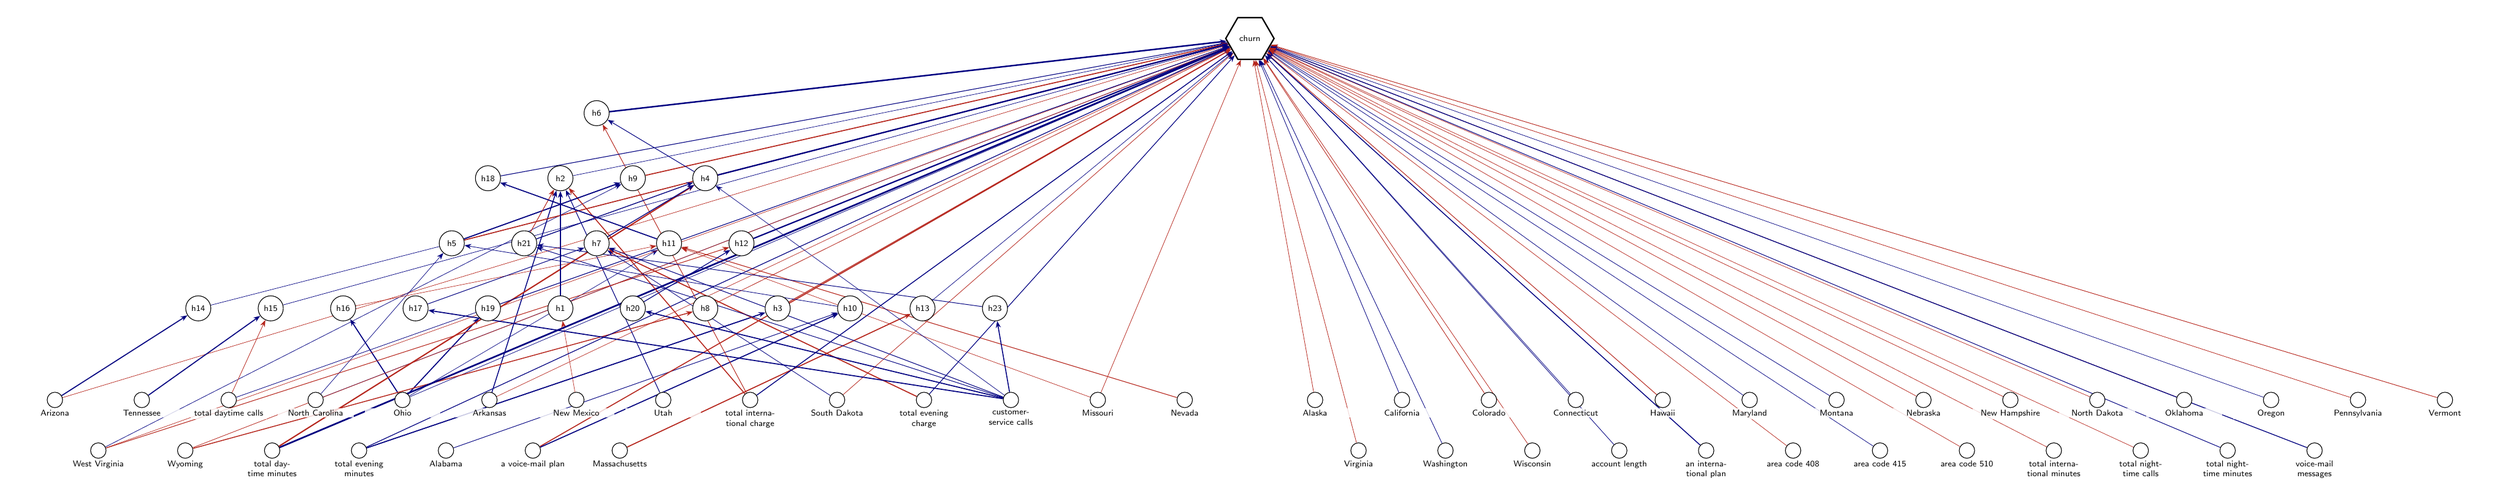
\begin{tikzpicture}[
  font=\sffamily\scriptsize, >={Stealth[length=1.4mm]},
  inp/.style={draw, circle, fill=white, minimum size=3.2mm, inner sep=0pt},
  hid/.style={draw, circle, fill=white, minimum size=5.2mm, inner sep=0.5pt, font=\sffamily\tiny},
  exitbox/.style={draw, thick, rectangle, fill=white, align=center, text width=17mm, minimum height=5mm, inner sep=1.5pt, font=\sffamily\tiny},
  sumbox/.style={draw, thick, dashed, rectangle, fill=white, align=center, text width=17mm, minimum height=5mm, inner sep=1.5pt, font=\sffamily\tiny},
  outp/.style={draw, thick, regular polygon, regular polygon sides=6, fill=white, minimum size=10mm, inner sep=0pt, font=\sffamily\tiny, align=center},
  stub/.style={draw, dashed, rounded corners=2pt, fill=white, align=center, inner sep=2pt, font=\sffamily\tiny, text width=15mm},
  inlab/.style={font=\sffamily\tiny, align=center, text width=15mm, inner sep=1pt, fill=white, fill opacity=0.8, text opacity=1},
  wpos/.style={draw=NavyBlue}, wneg/.style={draw=BrickRed}, wagg/.style={draw=black!45, line width=1.2pt},
  wmix/.style={draw=Plum},
]
\node[inp] (ninxxstatex0) at (26.1,0.0) {};
\path (ninxxstatex0.south) node[inlab, anchor=north] (labninxxstatex0) {Alaska};
\node[inp] (ninxxstatex19) at (11.7,-1.05) {};
\path (ninxxstatex19.south) node[inlab, anchor=north] (labninxxstatex19) {Massachusetts};
\node[inp] (ninxxstatex2) at (9.0,0.0) {};
\path (ninxxstatex2.south) node[inlab, anchor=north] (labninxxstatex2) {Arkansas};
\node[inp] (ninxxstatex20) at (35.1,0.0) {};
\path (ninxxstatex20.south) node[inlab, anchor=north] (labninxxstatex20) {Maryland};
\node[inp] (ninxxstatex24) at (21.6,0.0) {};
\path (ninxxstatex24.south) node[inlab, anchor=north] (labninxxstatex24) {Missouri};
\node[inp] (ninxxstatex1) at (8.1,-1.05) {};
\path (ninxxstatex1.south) node[inlab, anchor=north] (labninxxstatex1) {Alabama};
\node[inp] (ninxxstatex26) at (36.9,0.0) {};
\path (ninxxstatex26.south) node[inlab, anchor=north] (labninxxstatex26) {Montana};
\node[inp] (ninxxstatex27) at (5.4,0.0) {};
\path (ninxxstatex27.south) node[inlab, anchor=north] (labninxxstatex27) {North Carolina};
\node[inp] (ninxxstatex28) at (42.3,0.0) {};
\path (ninxxstatex28.south) node[inlab, anchor=north] (labninxxstatex28) {North Dakota};
\node[inp] (ninxxstatex29) at (38.7,0.0) {};
\path (ninxxstatex29.south) node[inlab, anchor=north] (labninxxstatex29) {Nebraska};
\node[inp] (ninxxstatex3) at (0.0,0.0) {};
\path (ninxxstatex3.south) node[inlab, anchor=north] (labninxxstatex3) {Arizona};
\node[inp] (ninxxstatex30) at (40.5,0.0) {};
\path (ninxxstatex30.south) node[inlab, anchor=north] (labninxxstatex30) {New Hampshire};
\node[inp] (ninxxstatex32) at (10.8,0.0) {};
\path (ninxxstatex32.south) node[inlab, anchor=north] (labninxxstatex32) {New Mexico};
\node[inp] (ninxxstatex33) at (23.4,0.0) {};
\path (ninxxstatex33.south) node[inlab, anchor=north] (labninxxstatex33) {Nevada};
\node[inp] (ninxxstatex35) at (7.2,0.0) {};
\path (ninxxstatex35.south) node[inlab, anchor=north] (labninxxstatex35) {Ohio};
\node[inp] (ninxxstatex36) at (44.1,0.0) {};
\path (ninxxstatex36.south) node[inlab, anchor=north] (labninxxstatex36) {Oklahoma};
\node[inp] (ninxxstatex37) at (45.9,0.0) {};
\path (ninxxstatex37.south) node[inlab, anchor=north] (labninxxstatex37) {Oregon};
\node[inp] (ninxxstatex38) at (47.7,0.0) {};
\path (ninxxstatex38.south) node[inlab, anchor=north] (labninxxstatex38) {Pennsylvania};
\node[inp] (ninxxstatex4) at (27.9,0.0) {};
\path (ninxxstatex4.south) node[inlab, anchor=north] (labninxxstatex4) {California};
\node[inp] (ninxxstatex41) at (16.2,0.0) {};
\path (ninxxstatex41.south) node[inlab, anchor=north] (labninxxstatex41) {South Dakota};
\node[inp] (ninxxstatex42) at (1.8,0.0) {};
\path (ninxxstatex42.south) node[inlab, anchor=north] (labninxxstatex42) {Tennessee};
\node[inp] (ninxxstatex11) at (33.3,0.0) {};
\path (ninxxstatex11.south) node[inlab, anchor=north] (labninxxstatex11) {Hawaii};
\node[inp] (ninxxstatex44) at (12.6,0.0) {};
\path (ninxxstatex44.south) node[inlab, anchor=north] (labninxxstatex44) {Utah};
\node[inp] (ninxxstatex45) at (27.0,-1.05) {};
\path (ninxxstatex45.south) node[inlab, anchor=north] (labninxxstatex45) {Virginia};
\node[inp] (ninxxstatex46) at (49.5,0.0) {};
\path (ninxxstatex46.south) node[inlab, anchor=north] (labninxxstatex46) {Vermont};
\node[inp] (ninxxstatex47) at (28.8,-1.05) {};
\path (ninxxstatex47.south) node[inlab, anchor=north] (labninxxstatex47) {Washington};
\node[inp] (ninxxstatex48) at (30.6,-1.05) {};
\path (ninxxstatex48.south) node[inlab, anchor=north] (labninxxstatex48) {Wisconsin};
\node[inp] (ninxxstatex49) at (0.9,-1.05) {};
\path (ninxxstatex49.south) node[inlab, anchor=north] (labninxxstatex49) {West Virginia};
\node[inp] (ninxxstatex5) at (29.7,0.0) {};
\path (ninxxstatex5.south) node[inlab, anchor=north] (labninxxstatex5) {Colorado};
\node[inp] (ninxxstatex50) at (2.7,-1.05) {};
\path (ninxxstatex50.south) node[inlab, anchor=north] (labninxxstatex50) {Wyoming};
\node[inp] (ninxxstatex6) at (31.5,0.0) {};
\path (ninxxstatex6.south) node[inlab, anchor=north] (labninxxstatex6) {Connecticut};
\node[inp] (ninxxaccountxlength) at (32.4,-1.05) {};
\path (ninxxaccountxlength.south) node[inlab, anchor=north] (labninxxaccountxlength) {account length};
\node[inp] (ninxxareaxcodex408) at (36.0,-1.05) {};
\path (ninxxareaxcodex408.south) node[inlab, anchor=north] (labninxxareaxcodex408) {area code 408};
\node[inp] (ninxxareaxcodex415) at (37.8,-1.05) {};
\path (ninxxareaxcodex415.south) node[inlab, anchor=north] (labninxxareaxcodex415) {area code 415};
\node[inp] (ninxxareaxcodex510) at (39.6,-1.05) {};
\path (ninxxareaxcodex510.south) node[inlab, anchor=north] (labninxxareaxcodex510) {area code 510};
\node[inp] (ninxxinternationalxplan) at (34.2,-1.05) {};
\path (ninxxinternationalxplan.south) node[inlab, anchor=north] (labninxxinternationalxplan) {an international plan};
\node[inp] (ninxxvoicexmailxplan) at (9.9,-1.05) {};
\path (ninxxvoicexmailxplan.south) node[inlab, anchor=north] (labninxxvoicexmailxplan) {a voice-mail plan};
\node[inp] (ninxxnumberxvmailxmessages) at (46.8,-1.05) {};
\path (ninxxnumberxvmailxmessages.south) node[inlab, anchor=north] (labninxxnumberxvmailxmessages) {voice-mail messages};
\node[inp] (ninxxtotalxdayxminutes) at (4.5,-1.05) {};
\path (ninxxtotalxdayxminutes.south) node[inlab, anchor=north] (labninxxtotalxdayxminutes) {total daytime minutes};
\node[inp] (ninxxtotalxdayxcalls) at (3.6,0.0) {};
\path (ninxxtotalxdayxcalls.south) node[inlab, anchor=north] (labninxxtotalxdayxcalls) {total daytime calls};
\node[inp] (ninxxtotalxevexminutes) at (6.3,-1.05) {};
\path (ninxxtotalxevexminutes.south) node[inlab, anchor=north] (labninxxtotalxevexminutes) {total evening minutes};
\node[inp] (ninxxtotalxevexcharge) at (18.0,0.0) {};
\path (ninxxtotalxevexcharge.south) node[inlab, anchor=north] (labninxxtotalxevexcharge) {total evening charge};
\node[inp] (ninxxtotalxnightxminutes) at (45.0,-1.05) {};
\path (ninxxtotalxnightxminutes.south) node[inlab, anchor=north] (labninxxtotalxnightxminutes) {total night-time minutes};
\node[inp] (ninxxtotalxnightxcalls) at (43.2,-1.05) {};
\path (ninxxtotalxnightxcalls.south) node[inlab, anchor=north] (labninxxtotalxnightxcalls) {total night-time calls};
\node[inp] (ninxxtotalxintlxminutes) at (41.4,-1.05) {};
\path (ninxxtotalxintlxminutes.south) node[inlab, anchor=north] (labninxxtotalxintlxminutes) {total international minutes};
\node[inp] (ninxxtotalxintlxcharge) at (14.4,0.0) {};
\path (ninxxtotalxintlxcharge.south) node[inlab, anchor=north] (labninxxtotalxintlxcharge) {total international charge};
\node[inp] (ninxxnumberxcustomerxservicexcalls) at (19.8,0.0) {};
\path (ninxxnumberxcustomerxservicexcalls.south) node[inlab, anchor=north] (labninxxnumberxcustomerxservicexcalls) {customer-service calls};
\node[outp] (n0) at (24.75,7.5) {churn};
\node[hid] (n10249) at (2.97,1.9) {h14};
\node[hid] (n1133) at (8.22,3.25) {h5};
\node[hid] (n11427) at (4.47,1.9) {h15};
\node[hid] (n11951) at (5.97,1.9) {h16};
\node[hid] (n1264) at (11.22,5.95) {h6};
\node[hid] (n12926) at (7.47,1.9) {h17};
\node[hid] (n13827) at (8.97,4.6) {h18};
\node[hid] (n14942) at (8.97,1.9) {h19};
\node[hid] (n161) at (10.47,1.9) {h1};
\node[hid] (n17032) at (11.97,1.9) {h20};
\node[hid] (n252) at (10.47,4.6) {h2};
\node[hid] (n2627) at (9.72,3.25) {h21};
\node[hid] (n2796) at (11.22,3.25) {h7};
\node[hid] (n3861) at (13.47,1.9) {h8};
\node[hid] (n4051) at (11.97,4.6) {h9};
\node[hid] (n476) at (14.97,1.9) {h3};
\node[hid] (n5577) at (16.47,1.9) {h10};
\node[hid] (n6730) at (12.72,3.25) {h11};
\node[hid] (n7208) at (14.22,3.25) {h12};
\node[hid] (n807) at (13.47,4.6) {h4};
\node[hid] (n8896) at (17.97,1.9) {h13};
\node[hid] (n9555) at (19.47,1.9) {h23};
\begin{scope}[on background layer]
\draw[->, wneg, line width=0.29pt] (ninxxstatex0) -- (n0);
\draw[->, wneg, line width=0.60pt] (ninxxstatex19) -- (n8896);
\draw[->, wneg, line width=0.25pt] (ninxxstatex2) -- (n0);
\draw[->, wpos, line width=0.52pt] (ninxxstatex2) -- (n252);
\draw[->, wpos, line width=0.28pt] (ninxxstatex20) -- (n0);
\draw[->, wneg, line width=0.28pt] (ninxxstatex24) -- (n0);
\draw[->, wneg, line width=0.25pt] (ninxxstatex24) -- (n6730);
\draw[->, wpos, line width=0.34pt] (ninxxstatex1) -- (n5577);
\draw[->, wpos, line width=0.28pt] (ninxxstatex26) -- (n0);
\draw[->, wpos, line width=0.26pt] (ninxxstatex27) -- (n0);
\draw[->, wpos, line width=0.26pt] (ninxxstatex27) -- (n1133);
\draw[->, wneg, line width=0.25pt] (ninxxstatex28) -- (n0);
\draw[->, wneg, line width=0.27pt] (ninxxstatex29) -- (n0);
\draw[->, wneg, line width=0.26pt] (ninxxstatex3) -- (n0);
\draw[->, wpos, line width=0.60pt] (ninxxstatex3) -- (n10249);
\draw[->, wneg, line width=0.27pt] (ninxxstatex30) -- (n0);
\draw[->, wneg, line width=0.25pt] (ninxxstatex32) -- (n161);
\draw[->, wneg, line width=0.40pt] (ninxxstatex33) -- (n6730);
\draw[->, wpos, line width=0.26pt] (ninxxstatex35) -- (n0);
\draw[->, wpos, line width=0.60pt] (ninxxstatex35) -- (n11951);
\draw[->, wpos, line width=0.60pt] (ninxxstatex35) -- (n14942);
\draw[->, wpos, line width=0.25pt] (ninxxstatex35) -- (n6730);
\draw[->, wneg, line width=0.26pt] (ninxxstatex36) -- (n0);
\draw[->, wpos, line width=0.26pt] (ninxxstatex37) -- (n0);
\draw[->, wneg, line width=0.29pt] (ninxxstatex38) -- (n0);
\draw[->, wpos, line width=0.30pt] (ninxxstatex4) -- (n0);
\draw[->, wneg, line width=0.29pt] (ninxxstatex41) -- (n0);
\draw[->, wpos, line width=0.30pt] (ninxxstatex41) -- (n2796);
\draw[->, wpos, line width=0.60pt] (ninxxstatex42) -- (n11427);
\draw[->, wneg, line width=0.36pt] (ninxxstatex11) -- (n0);
\draw[->, wpos, line width=0.40pt] (ninxxstatex44) -- (n252);
\draw[->, wneg, line width=0.29pt] (ninxxstatex45) -- (n0);
\draw[->, wneg, line width=0.34pt] (ninxxstatex46) -- (n0);
\draw[->, wpos, line width=0.30pt] (ninxxstatex47) -- (n0);
\draw[->, wneg, line width=0.28pt] (ninxxstatex48) -- (n0);
\draw[->, wneg, line width=0.25pt] (ninxxstatex49) -- (n0);
\draw[->, wpos, line width=0.27pt] (ninxxstatex49) -- (n4051);
\draw[->, wneg, line width=0.38pt] (ninxxstatex49) -- (n7208);
\draw[->, wneg, line width=0.32pt] (ninxxstatex5) -- (n0);
\draw[->, wneg, line width=0.29pt] (ninxxstatex50) -- (n0);
\draw[->, wneg, line width=0.52pt] (ninxxstatex50) -- (n3861);
\draw[->, wpos, line width=0.26pt] (ninxxstatex6) -- (n0);
\draw[->, wpos, line width=0.30pt] (ninxxaccountxlength) -- (n0);
\draw[->, wneg, line width=0.26pt] (ninxxareaxcodex408) -- (n0);
\draw[->, wpos, line width=0.27pt] (ninxxareaxcodex415) -- (n0);
\draw[->, wneg, line width=0.26pt] (ninxxareaxcodex510) -- (n0);
\draw[->, wpos, line width=0.51pt] (ninxxinternationalxplan) -- (n0);
\draw[->, wneg, line width=0.56pt] (ninxxvoicexmailxplan) -- (n0);
\draw[->, wpos, line width=0.60pt] (ninxxvoicexmailxplan) -- (n5577);
\draw[->, wpos, line width=0.47pt] (ninxxnumberxvmailxmessages) -- (n0);
\draw[->, wpos, line width=0.96pt] (ninxxtotalxdayxminutes) -- (n0);
\draw[->, wneg, line width=0.74pt] (ninxxtotalxdayxminutes) -- (n807);
\draw[->, wpos, line width=0.29pt] (ninxxtotalxdayxcalls) -- (n0);
\draw[->, wneg, line width=0.29pt] (ninxxtotalxdayxcalls) -- (n11427);
\draw[->, wpos, line width=0.43pt] (ninxxtotalxevexminutes) -- (n0);
\draw[->, wpos, line width=0.63pt] (ninxxtotalxevexminutes) -- (n476);
\draw[->, wpos, line width=0.41pt] (ninxxtotalxevexcharge) -- (n0);
\draw[->, wneg, line width=0.60pt] (ninxxtotalxevexcharge) -- (n2796);
\draw[->, wpos, line width=0.36pt] (ninxxtotalxnightxminutes) -- (n0);
\draw[->, wneg, line width=0.25pt] (ninxxtotalxnightxcalls) -- (n0);
\draw[->, wneg, line width=0.26pt] (ninxxtotalxintlxminutes) -- (n0);
\draw[->, wpos, line width=0.50pt] (ninxxtotalxintlxcharge) -- (n0);
\draw[->, wneg, line width=0.36pt] (ninxxtotalxintlxcharge) -- (n1264);
\draw[->, wneg, line width=0.55pt] (ninxxtotalxintlxcharge) -- (n252);
\draw[->, wpos, line width=0.60pt] (ninxxnumberxcustomerxservicexcalls) -- (n12926);
\draw[->, wpos, line width=0.60pt] (ninxxnumberxcustomerxservicexcalls) -- (n17032);
\draw[->, wpos, line width=0.35pt] (ninxxnumberxcustomerxservicexcalls) -- (n2627);
\draw[->, wpos, line width=0.38pt] (ninxxnumberxcustomerxservicexcalls) -- (n2796);
\draw[->, wpos, line width=0.26pt] (ninxxnumberxcustomerxservicexcalls) -- (n807);
\draw[->, wpos, line width=0.55pt] (ninxxnumberxcustomerxservicexcalls) -- (n9555);
\draw[->, wpos, line width=0.26pt] (n10249) -- (n0);
\draw[->, wneg, line width=0.58pt] (n1133) -- (n0);
\draw[->, wpos, line width=0.65pt] (n1133) -- (n4051);
\draw[->, wpos, line width=0.27pt] (n11427) -- (n0);
\draw[->, wneg, line width=0.25pt] (n11951) -- (n6730);
\draw[->, wpos, line width=0.88pt] (n1264) -- (n0);
\draw[->, wpos, line width=0.37pt] (n12926) -- (n2796);
\draw[->, wpos, line width=0.40pt] (n13827) -- (n0);
\draw[->, wpos, line width=0.26pt] (n14942) -- (n0);
\draw[->, wpos, line width=0.53pt] (n161) -- (n252);
\draw[->, wpos, line width=0.44pt] (n17032) -- (n7208);
\draw[->, wpos, line width=0.26pt] (n252) -- (n0);
\draw[->, wneg, line width=0.38pt] (n2627) -- (n252);
\draw[->, wpos, line width=0.49pt] (n2627) -- (n807);
\draw[->, wpos, line width=0.47pt] (n2796) -- (n807);
\draw[->, wneg, line width=0.30pt] (n3861) -- (n0);
\draw[->, wneg, line width=0.60pt] (n4051) -- (n0);
\draw[->, wneg, line width=0.44pt] (n476) -- (n0);
\draw[->, wpos, line width=0.30pt] (n5577) -- (n1133);
\draw[->, wpos, line width=0.60pt] (n6730) -- (n13827);
\draw[->, wpos, line width=0.77pt] (n7208) -- (n0);
\draw[->, wpos, line width=0.81pt] (n807) -- (n0);
\draw[->, wpos, line width=0.38pt] (n807) -- (n1264);
\draw[->, wpos, line width=0.26pt] (n8896) -- (n0);
\draw[->, wpos, line width=0.36pt] (n9555) -- (n2627);
\end{scope}
\end{tikzpicture}}%
\caption{The network as trained, before any explanation, in full. Blue: positive weight (raises the score); red: negative weight (lowers it); thicker: larger weight. Orange outline and up arrow: raises the final prediction; teal and down arrow: lowers it; grey and double arrow: depends. Not used (no connection): Georgia, Iowa, Idaho, Illinois, Indiana, Kansas, Kentucky, Louisiana, Maine, Michigan, Minnesota, Mississippi, New Jersey, New York, Rhode Island, South Carolina, Texas, Washington DC, Delaware, Florida, total daytime charge, total evening calls, total night-time charge, total international calls.}
\label{fig:churn100s2c1:raw}
\end{figure}
\end{landscape}
\end{drafted}
\clearpage
\begin{drafted}[plain-language layer: churn100-s2-c2]
\section{churn100-s2-c2}
\noindent{\small Genome \texttt{e5394267-5807-44ae-8629-5e157bcfb43a}, explanation \texttt{4792056e-ee3e-4fde-a1bb-4c4d809e2d61}. Split: train primary (n=4000), test as a check (n=1000). Claims: 147, verified 138, not supported 9.\par}
\noindent{\small\textcolor{BrickRed}{AI-assisted draft for review (unverified)}\par}\smallskip
\noindent{\footnotesize Reference (typical) customer: the typical customer: the median training customer for every number and the most common training category for every category (not a real customer). account length: 100; area code: area code 415; international plan: no international plan; number customer service calls: 1 calls; number vmail messages: 0 messages; state: West Virginia; total day calls: 100 calls; total day charge: 30.69 US dollars; total day minutes: 180 minutes; total eve calls: 100 calls; total eve charge: 17.12 US dollars; total eve minutes: 201 minutes; total intl calls: 4 calls; total intl charge: 2.78 US dollars; total intl minutes: 10 minutes; total night calls: 100 calls; total night charge: 9.02 US dollars; total night minutes: 200 minutes; voice mail plan: no voice-mail plan. Predicted chance that a customer leaves: 1\%.\par}
\subsection{Summary}
\noindent For a typical customer (in West Virginia, area code 415, no international or voice-mail plan, 1 call to customer service and median usage) the model predicts a chance of leaving of about 1\%; it adds up six parts: fixed-weight inputs, service calls, a voice-mail discount, state units, an area-code unit and a small Utah unit.\,{\scriptsize\textcolor{NavyBlue}{[C051]}} Figure~\ref{fig:churn100s2c2:summary} shows the model at this level: one box per paragraph below.
\par\medskip\noindent\fbox{\begin{minipage}{0.96\linewidth}\small\textbf{How to read the diagrams.} Edge colour is the sign of that one connection: blue positive, red negative; thicker is a larger weight. The outline and arrow on an input (and on a part's output box) is its overall effect on the final prediction, read from the verified claims: orange and up arrow raises it, teal and down arrow lowers it, grey and double arrow depends (it goes both ways, or differs between levels). A negative connection into a part that itself raises the prediction means that input lowers the prediction; through a hinge the overall effect can only be read from the claims, not from the edges. Up arrow means towards churn; down arrow, away from it. A double outline marks an input (or a part's output) that acts at a fixed rate everywhere: it adds the same amount to the score per unit, so it is explained by its rate alone (see 'Linear factors'); a dashed double outline, at a fixed rate on the observed data. The normal outline is an input whose effect switches on and off somewhere. For example, total daytime minutes has a negative connection into 'Service calls', a part that raises the predicted chance that a customer leaves, so total daytime minutes lowers it.\end{minipage}}\par\medskip
\begin{figure}[H]\centering
\resizebox{!}{\ifdim\height>0.5\textheight 0.5\textheight\else\height\fi}{%
\resizebox{\ifdim\width>\linewidth\linewidth\else\width\fi}{!}{%
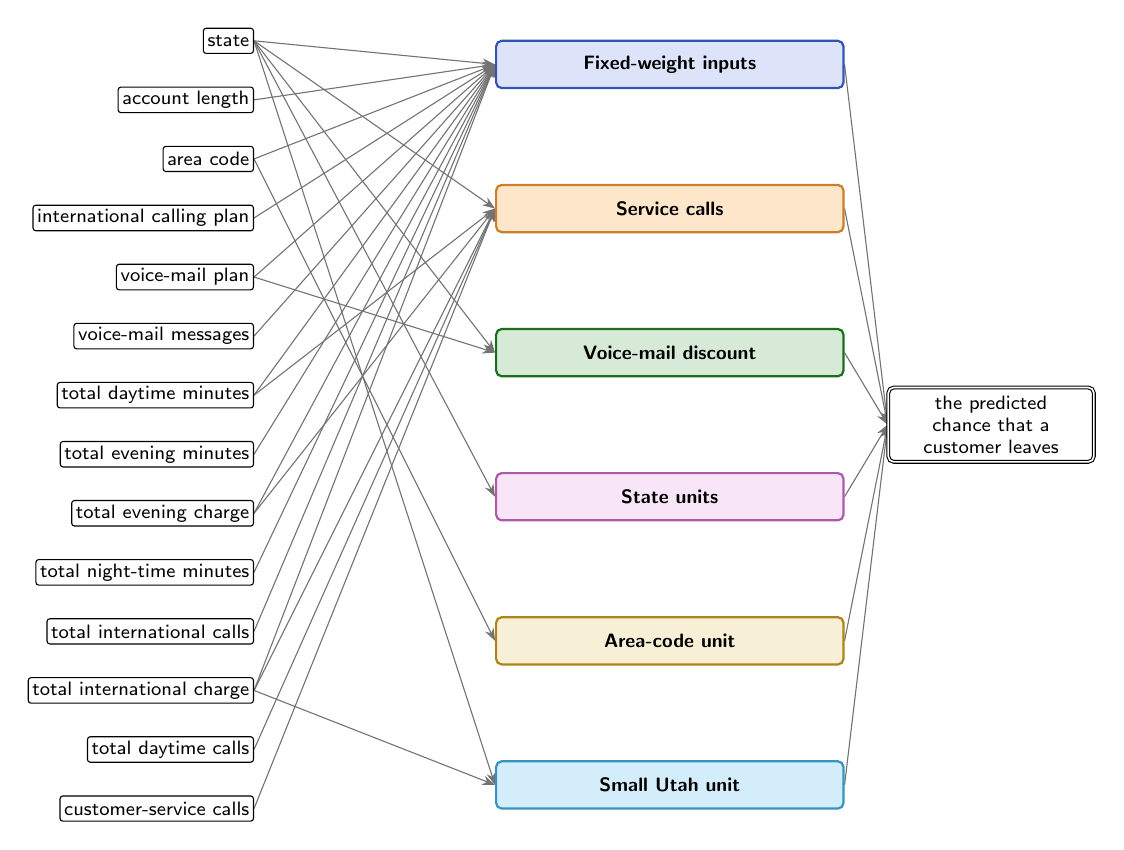
\begin{tikzpicture}[
  font=\sffamily\scriptsize, >={Stealth[length=1.6mm]},
  inp/.style={draw, rounded corners=1pt, fill=white, inner sep=1.5pt, minimum height=3.2mm, anchor=east},
  abox/.style={draw, thick, rounded corners=2pt, align=center, inner sep=3pt, minimum height=6mm, text width=42mm},
  outp/.style={draw, double, rounded corners=2pt, fill=white, align=center, inner sep=3pt, text width=24mm},
  agg/.style={draw=black!55},
]
\node[inp] (i0) at (0,4.875) {state};
\node[inp] (i1) at (0,4.125) {account length};
\node[inp] (i2) at (0,3.375) {area code};
\node[inp] (i3) at (0,2.625) {international calling plan};
\node[inp] (i4) at (0,1.875) {voice-mail plan};
\node[inp] (i5) at (0,1.125) {voice-mail messages};
\node[inp] (i6) at (0,0.375) {total daytime minutes};
\node[inp] (i7) at (0,-0.375) {total evening minutes};
\node[inp] (i8) at (0,-1.125) {total evening charge};
\node[inp] (i9) at (0,-1.875) {total night-time minutes};
\node[inp] (i10) at (0,-2.625) {total international calls};
\node[inp] (i11) at (0,-3.375) {total international charge};
\node[inp] (i12) at (0,-4.125) {total daytime calls};
\node[inp] (i13) at (0,-4.875) {customer-service calls};
\node[abox, fill=RoyalBlue!18, draw=RoyalBlue!80!black] (b0) at (5.28,4.575) {\textbf{Fixed-weight inputs}};
\node[abox, fill=BurntOrange!18, draw=BurntOrange!80!black] (b1) at (5.28,2.745) {\textbf{Service calls}};
\node[abox, fill=ForestGreen!18, draw=ForestGreen!80!black] (b2) at (5.28,0.915) {\textbf{Voice-mail discount}};
\node[abox, fill=Orchid!18, draw=Orchid!80!black] (b3) at (5.28,-0.915) {\textbf{State units}};
\node[abox, fill=Goldenrod!18, draw=Goldenrod!80!black] (b4) at (5.28,-2.745) {\textbf{Area-code unit}};
\node[abox, fill=Cerulean!18, draw=Cerulean!80!black] (b5) at (5.28,-4.575) {\textbf{Small Utah unit}};
\node[outp] (out) at (9.36,0) {the predicted chance that a customer leaves};
\begin{scope}[on background layer]
\draw[->, agg, thin] (i0.east) -- (b0.west);
\draw[->, agg, thin] (i1.east) -- (b0.west);
\draw[->, agg, thin] (i2.east) -- (b0.west);
\draw[->, agg, thin] (i3.east) -- (b0.west);
\draw[->, agg, thin] (i4.east) -- (b0.west);
\draw[->, agg, thin] (i5.east) -- (b0.west);
\draw[->, agg, thin] (i6.east) -- (b0.west);
\draw[->, agg, thin] (i7.east) -- (b0.west);
\draw[->, agg, thin] (i8.east) -- (b0.west);
\draw[->, agg, thin] (i9.east) -- (b0.west);
\draw[->, agg, thin] (i10.east) -- (b0.west);
\draw[->, agg, thin] (i11.east) -- (b0.west);
\draw[->, agg] (b0.east) -- (out.west);
\draw[->, agg, thin] (i0.east) -- (b1.west);
\draw[->, agg, thin] (i6.east) -- (b1.west);
\draw[->, agg, thin] (i12.east) -- (b1.west);
\draw[->, agg, thin] (i8.east) -- (b1.west);
\draw[->, agg, thin] (i11.east) -- (b1.west);
\draw[->, agg, thin] (i13.east) -- (b1.west);
\draw[->, agg] (b1.east) -- (out.west);
\draw[->, agg, thin] (i0.east) -- (b2.west);
\draw[->, agg, thin] (i4.east) -- (b2.west);
\draw[->, agg] (b2.east) -- (out.west);
\draw[->, agg, thin] (i0.east) -- (b3.west);
\draw[->, agg] (b3.east) -- (out.west);
\draw[->, agg, thin] (i2.east) -- (b4.west);
\draw[->, agg] (b4.east) -- (out.west);
\draw[->, agg, thin] (i0.east) -- (b5.west);
\draw[->, agg, thin] (i11.east) -- (b5.west);
\draw[->, agg] (b5.east) -- (out.west);
\end{scope}
\end{tikzpicture}}}%
\caption{The model at the level of the summary: one box per part.}
\label{fig:churn100s2c2:summary}
\end{figure}
\paragraph{Fixed-weight inputs.} This part adds up most inputs with fixed weights, and daytime minutes count most: they raise a typical customer's chance of leaving steadily, from under 1\% at 112 to about 11\% at 249 minutes.\,{\scriptsize\textcolor{NavyBlue}{[C053]}} An international plan takes the chance from about 1\% to about 14\%, a voice-mail plan lowers it to under 1\%, and more voice-mail messages raise it steadily, from about 1\% at 0 to about 4\% at 32 messages.\,{\scriptsize\textcolor{NavyBlue}{[C052, C061, C056]}} A higher international charge, more evening minutes, a higher evening charge and more night-time minutes also raise it steadily, each by one to two points.\,{\scriptsize\textcolor{NavyBlue}{[C057, C059, C060, C065]}} Through it, the state moves the chance from about 1\% in West Virginia to about 5\% in Washington and in California, and to under 1\% in Hawaii (41 to 122 training customers per state).\,{\scriptsize\textcolor{NavyBlue}{[C054, C055, C062]}}
\paragraph{Service calls.} This part adds up two parts: customer-service calls combined with low daytime use, and a rise from 4 calls upwards.\,{\scriptsize\textcolor{NavyBlue}{[C103]}} Through it, daytime minutes lower the chance only while they stay below about 166 minutes (between 145 and 213 minutes for different customers), in an uneven way: for a typical such customer, from about 28\% at 91 minutes to about 1\% at 352 minutes.\,{\scriptsize\textcolor{NavyBlue}{[C098]}} With an evening charge above 17.12 US dollars, the chance is lowest at about 148 minutes of daytime use and higher either side: from about 1\% at 112 minutes to about 13\% at 249 minutes, against about 2\% to about 9\% at or below that charge.\,{\scriptsize\textcolor{NavyBlue}{[C095]}} Customer-service calls add to it from 4 calls upwards, slowly at first, then faster: for a typical such customer, from about 3\% at 0 calls to about 8\% at 4 calls.\,{\scriptsize\textcolor{NavyBlue}{[C099]}}
\paragraph{Voice-mail discount.} This part reads the voice-mail plan and one state: through it, a voice-mail plan lowers a typical customer's chance from about 1\% to under 1\%, and customers in North Carolina get under 1\% instead of about 1\%.\,{\scriptsize\textcolor{NavyBlue}{[C119, C120]}}
\paragraph{State units.} This part reads only the state: it raises a typical customer's chance from about 1\% to about 2\% in Washington and in Montana, and by less than a point in Kentucky and Ohio.\,{\scriptsize\textcolor{NavyBlue}{[C125, C126, C127, C128]}}
\paragraph{Area-code unit.} This part reads the area code and barely changes the predictions (by at most half a point).\,{\scriptsize\textcolor{NavyBlue}{[C137]}}
\paragraph{Small Utah unit.} This small part reads the international charge and being in Utah, and barely changes the predictions (by at most 0.2 points).\,{\scriptsize\textcolor{NavyBlue}{[C144]}}
\paragraph{The whole network.} Figure~\ref{fig:churn100s2c2:overview} (next page, landscape) draws every unit and connection of the explained model, nested by part: shaded clusters are the parts of the model and darker boxes the parts inside them; circles are hidden units (h1, h2, \ldots); each cluster's rectangle is its output, and a dashed `sum' stands for an addition the next unit does (drawn, not a unit of the model); the hexagon is the model's output. An input used by several parts is drawn under each of them (same label, dotted outline, the first copy marked with the number of copies): it is the same input, repeated for readability. Not used by the model (input columns with no connection): state: 25 of 51 levels, total daytime charge, total evening calls, total night-time calls, total night-time charge, total international minutes.
\begin{landscape}
\begin{figure}[p]\centering
\resizebox{\linewidth}{!}{%
\definecolor{netup}{HTML}{D95F02}\definecolor{netdown}{HTML}{1B9E77}\definecolor{netmixed}{HTML}{7F7F7F}%
\begin{tikzpicture}[
  font=\sffamily\scriptsize, >={Stealth[length=1.4mm]},
  inp/.style={draw, circle, fill=white, minimum size=3.2mm, inner sep=0pt},
  hid/.style={draw, circle, fill=white, minimum size=5.2mm, inner sep=0.5pt, font=\sffamily\tiny},
  exitbox/.style={draw, thick, rectangle, fill=white, align=center, text width=17mm, minimum height=5mm, inner sep=1.5pt, font=\sffamily\tiny},
  sumbox/.style={draw, thick, dashed, rectangle, fill=white, align=center, text width=17mm, minimum height=5mm, inner sep=1.5pt, font=\sffamily\tiny},
  outp/.style={draw, thick, regular polygon, regular polygon sides=6, fill=white, minimum size=10mm, inner sep=0pt, font=\sffamily\tiny, align=center},
  stub/.style={draw, dashed, rounded corners=2pt, fill=white, align=center, inner sep=2pt, font=\sffamily\tiny, text width=15mm},
  inlab/.style={font=\sffamily\tiny, align=center, text width=15mm, inner sep=1pt, fill=white, fill opacity=0.8, text opacity=1},
  wpos/.style={draw=NavyBlue}, wneg/.style={draw=BrickRed}, wagg/.style={draw=black!45, line width=1.2pt},
  wmix/.style={draw=Plum},
]
\node[outp] (n0) at (26.2,8.85) {churn};
\node[hid] (n10332) at (31.27,1.9) {h16};
\node[hid] (n11261) at (32.77,1.9) {h17};
\node[hid] (n1133) at (27.48,3.25) {h4};
\node[hid] (n1264) at (15.31,5.95) {h5};
\node[hid] (n13551) at (34.27,1.9) {h18};
\node[hid] (n13725) at (35.77,1.9) {h19};
\node[hid] (n13852) at (25.98,1.9) {h20};
\node[hid] (n14653) at (44.71,1.9) {h21};
\node[hid] (n14955) at (27.48,1.9) {h22};
\node[hid] (n15509) at (14.56,1.9) {h23};
\node[hid] (n161) at (46.21,1.9) {h1};
\node[hid] (n16344) at (37.27,1.9) {h24};
\node[hid] (n16902) at (35.77,3.25) {h25};
\node[exitbox] (n252) at (50.6,1.9) {Small Utah unit $\uparrow$};
\node[hid] (n2627) at (14.56,3.25) {h6};
\node[hid] (n2796) at (16.06,3.25) {h7};
\node[hid] (n4051) at (27.48,4.6) {h8};
\node[hid] (n4967) at (38.77,1.9) {h9};
\node[hid] (n5577) at (28.98,1.9) {h10};
\node[hid] (n7208) at (19.14,1.9) {h11};
\node[hid] (n7647) at (37.27,3.25) {h12};
\node[hid] (n807) at (15.31,4.6) {h3};
\node[hid] (n8418) at (40.27,1.9) {h13};
\node[hid] (n8896) at (41.77,1.9) {h14};
\node[hid] (n9555) at (16.06,1.9) {h15};
\node[exitbox] (nidentityxlin) at (5.85,1.9) {Fixed-weight inputs $\uparrow$};
\node[exitbox] (nidentityxsvc) at (22.47,7.3) {Service calls $\uparrow$};
\node[sumbox] (ncsumxxannx92) at (27.48,5.95) {sum: Voice-mail discount $\downarrow$};
\node[sumbox] (ncsumxxannx94) at (45.46,3.25) {sum: Area-code unit $\updownarrow$};
\node[sumbox] (ncsumxxannx95) at (36.52,4.6) {sum: State units $\updownarrow$};
\node[inp, densely dotted, thick, draw=netmixed, very thick] (ngrpxxstatexxannx93) at (49.7,0.0) {};
\path (ngrpxxstatexxannx93.south) node[inlab, anchor=north] (labngrpxxstatexxannx93) {state (26 of 51 used) ($\times$5) $\updownarrow$};
\node[inp, draw=netup, very thick] (ninxxareaxcodex415xxannx94) at (46.36,0.0) {};
\path (ninxxareaxcodex415xxannx94.south) node[inlab, anchor=north] (labninxxareaxcodex415xxannx94) {area code 415 $\uparrow$};
\node[inp, draw=netup, very thick] (ninxxtotalxdayxcallsxxannx96) at (14.14,0.0) {};
\path (ninxxtotalxdayxcallsxxannx96.south) node[inlab, anchor=north] (labninxxtotalxdayxcallsxxannx96) {total daytime calls $\uparrow$};
\node[inp, densely dotted, thick, draw=netmixed, very thick] (ngrpxxstatexxannx95) at (36.52,0.0) {};
\path (ngrpxxstatexxannx95.south) node[inlab, anchor=north] (labngrpxxstatexxannx95) {state (26 of 51 used) $\updownarrow$};
\node[inp, draw=netdown, very thick] (ninxxareaxcodex408xxannx94) at (44.56,0.0) {};
\path (ninxxareaxcodex408xxannx94.south) node[inlab, anchor=north] (labninxxareaxcodex408xxannx94) {area code 408 $\downarrow$};
\node[inp, draw=netup, very thick] (ninxxnumberxcustomerxservicexcallsxxannx96) at (23.14,0.0) {};
\path (ninxxnumberxcustomerxservicexcallsxxannx96.south) node[inlab, anchor=north] (labninxxnumberxcustomerxservicexcallsxxannx96) {customer-service calls $\uparrow$};
\node[inp, densely dotted, thick, draw=netdown, very thick] (ninxxtotalxintlxchargexxannx93) at (51.5,0.0) {};
\path (ninxxtotalxintlxchargexxannx93.south) node[inlab, anchor=north] (labninxxtotalxintlxchargexxannx93) {total international charge ($\times$3) $\downarrow$};
\node[inp, densely dotted, thick, draw=netdown, very thick] (ninxxtotalxintlxchargexxannx96) at (17.74,0.0) {};
\path (ninxxtotalxintlxchargexxannx96.south) node[inlab, anchor=north] (labninxxtotalxintlxchargexxannx96) {total international charge $\downarrow$};
\node[inp, densely dotted, thick, draw=netdown, very thick] (ninxxtotalxevexchargexxannx96) at (21.34,0.0) {};
\path (ninxxtotalxevexchargexxannx96.south) node[inlab, anchor=north] (labninxxtotalxevexchargexxannx96) {total evening charge ($\times$2) $\downarrow$};
\node[inp, densely dotted, thick, draw=netdown, very thick] (ninxxtotalxdayxminutesxxannx96) at (15.94,0.0) {};
\path (ninxxtotalxdayxminutesxxannx96.south) node[inlab, anchor=north] (labninxxtotalxdayxminutesxxannx96) {total daytime minutes ($\times$2) $\downarrow$};
\node[inp, densely dotted, thick, draw=netmixed, very thick] (ngrpxxstatexxannx96) at (19.54,0.0) {};
\path (ngrpxxstatexxannx96.south) node[inlab, anchor=north] (labngrpxxstatexxannx96) {state (26 of 51 used) $\updownarrow$};
\node[inp, densely dotted, thick, draw=netmixed, very thick] (ngrpxxstatexxannx92) at (28.38,0.0) {};
\path (ngrpxxstatexxannx92.south) node[inlab, anchor=north] (labngrpxxstatexxannx92) {state (26 of 51 used) $\updownarrow$};
\node[inp, densely dotted, thick, draw=netdown, very thick] (ninxxvoicexmailxplanxxannx92) at (26.58,0.0) {};
\path (ninxxvoicexmailxplanxxannx92.south) node[inlab, anchor=north] (labninxxvoicexmailxplanxxannx92) {a voice-mail plan ($\times$2) $\downarrow$};
\node[inp, densely dotted, thick, draw=netmixed, very thick] (ngrpxxstatexxannx89) at (4.5,0.0) {};
\path (ngrpxxstatexxannx89.south) node[inlab, anchor=north] (labngrpxxstatexxannx89) {state (26 of 51 used) $\updownarrow$};
\node[inp, draw=netup, very thick] (ninxxaccountxlengthxxannx89) at (1.8,-1.05) {};
\path (ninxxaccountxlengthxxannx89.south) node[inlab, anchor=north] (labninxxaccountxlengthxxannx89) {account length $\uparrow$};
\node[inp, draw=netdown, very thick] (ninxxareaxcodex510xxannx89) at (3.6,-1.05) {};
\path (ninxxareaxcodex510xxannx89.south) node[inlab, anchor=north] (labninxxareaxcodex510xxannx89) {area code 510 $\downarrow$};
\node[inp, draw=netup, very thick] (ninxxinternationalxplanxxannx89) at (2.7,0.0) {};
\path (ninxxinternationalxplanxxannx89.south) node[inlab, anchor=north] (labninxxinternationalxplanxxannx89) {an international plan $\uparrow$};
\node[inp, draw=netup, very thick] (ninxxnumberxvmailxmessagesxxannx89) at (10.8,-1.05) {};
\path (ninxxnumberxvmailxmessagesxxannx89.south) node[inlab, anchor=north] (labninxxnumberxvmailxmessagesxxannx89) {voice-mail messages $\uparrow$};
\node[inp, draw=netup, very thick] (ninxxtotalxevexminutesxxannx89) at (7.2,-1.05) {};
\path (ninxxtotalxevexminutesxxannx89.south) node[inlab, anchor=north] (labninxxtotalxevexminutesxxannx89) {total evening minutes $\uparrow$};
\node[inp, draw=netup, very thick] (ninxxtotalxnightxminutesxxannx89) at (9.9,0.0) {};
\path (ninxxtotalxnightxminutesxxannx89.south) node[inlab, anchor=north] (labninxxtotalxnightxminutesxxannx89) {total night-time minutes $\uparrow$};
\node[inp, draw=netdown, very thick] (ninxxtotalxintlxcallsxxannx89) at (8.1,0.0) {};
\path (ninxxtotalxintlxcallsxxannx89.south) node[inlab, anchor=north] (labninxxtotalxintlxcallsxxannx89) {total international calls $\downarrow$};
\node[inp, densely dotted, thick, draw=netup, very thick] (ninxxtotalxintlxchargexxannx89) at (9.0,-1.05) {};
\path (ninxxtotalxintlxchargexxannx89.south) node[inlab, anchor=north] (labninxxtotalxintlxchargexxannx89) {total international charge $\uparrow$};
\node[inp, densely dotted, thick, draw=netup, very thick] (ninxxtotalxevexchargexxannx89) at (6.3,0.0) {};
\path (ninxxtotalxevexchargexxannx89.south) node[inlab, anchor=north] (labninxxtotalxevexchargexxannx89) {total evening charge $\uparrow$};
\node[inp, densely dotted, thick, draw=netup, very thick] (ninxxtotalxdayxminutesxxannx89) at (5.4,-1.05) {};
\path (ninxxtotalxdayxminutesxxannx89.south) node[inlab, anchor=north] (labninxxtotalxdayxminutesxxannx89) {total daytime minutes $\uparrow$};
\node[inp, densely dotted, thick, draw=netdown, very thick] (ninxxvoicexmailxplanxxannx89) at (0.9,0.0) {};
\path (ninxxvoicexmailxplanxxannx89.south) node[inlab, anchor=north] (labninxxvoicexmailxplanxxannx89) {a voice-mail plan $\downarrow$};
\node[font=\sffamily\tiny\bfseries, text=ForestGreen!60!black, inner sep=1pt] (subt0) at (15.31,6.45) {Calls with low usage};
\node[font=\sffamily\tiny\bfseries, text=ForestGreen!60!black, inner sep=1pt] (subt1) at (19.14,2.4) {Many service calls};
\begin{scope}[on background layer]
\node[fit=(nidentityxlin) , inner sep=8pt, rounded corners=5pt, fill=BurntOrange!10, draw=BurntOrange!45] (clu1) {};
\node[fit=(n1264) (n15509) (n2627) (n2796) (n7208) (n807) (n9555) (nidentityxsvc) (subt0) (subt1), inner sep=8pt, rounded corners=5pt, fill=ForestGreen!10, draw=ForestGreen!45] (clu2) {};
\node[fit=(n1133) (n13852) (n14955) (n4051) (n5577) (ncsumxxannx92) , inner sep=8pt, rounded corners=5pt, fill=Orchid!10, draw=Orchid!45] (clu3) {};
\node[fit=(n10332) (n11261) (n13551) (n13725) (n16344) (n16902) (n4967) (n7647) (n8418) (n8896) (ncsumxxannx95) , inner sep=8pt, rounded corners=5pt, fill=Goldenrod!10, draw=Goldenrod!45] (clu4) {};
\node[fit=(n14653) (n161) (ncsumxxannx94) , inner sep=8pt, rounded corners=5pt, fill=Cerulean!10, draw=Cerulean!45] (clu5) {};
\node[fit=(n252) , inner sep=8pt, rounded corners=5pt, fill=Mahogany!10, draw=Mahogany!45] (clu6) {};
\node[fit=(n1264) (n15509) (n2627) (n2796) (n807) (n9555) (subt0), inner sep=4pt, rounded corners=3pt, fill=ForestGreen!26, draw=ForestGreen!70] {};
\node[fit=(n7208) (subt1), inner sep=4pt, rounded corners=3pt, fill=ForestGreen!26, draw=ForestGreen!70] {};
\draw[->, wpos, line width=0.27pt] (n161) -- (ncsumxxannx94);
\draw[->, wpos, line width=0.25pt] (n252) -- (n0);
\draw[->, wneg, line width=0.56pt] (n1133) -- (ncsumxxannx92);
\draw[->, wneg, line width=0.60pt] (n4051) -- (ncsumxxannx92);
\draw[->, wneg, line width=0.25pt] (n7647) -- (ncsumxxannx95);
\draw[->, wneg, line width=0.25pt] (n8418) -- (ncsumxxannx95);
\draw[->, wneg, line width=0.25pt] (n8896) -- (ncsumxxannx95);
\draw[->, wpos, line width=0.45pt] (ninxxareaxcodex415xxannx94) -- (n161);
\draw[->, wpos, line width=0.27pt] (ninxxtotalxdayxcallsxxannx96) -- (n807);
\draw[->, wpos, line width=0.29pt] (n10332) -- (ncsumxxannx95);
\draw[->, wpos, line width=0.27pt] (n13551) -- (ncsumxxannx95);
\draw[->, wpos, line width=0.27pt] (n13725) -- (ncsumxxannx95);
\draw[->, wneg, line width=0.34pt] (n14653) -- (ncsumxxannx94);
\draw[->, wpos, line width=0.27pt] (n16344) -- (ncsumxxannx95);
\draw[->, wpos, line width=0.27pt] (n16902) -- (ncsumxxannx95);
\draw[->, wpos, line width=0.46pt] (n2627) -- (n807);
\draw[->, wpos, line width=0.45pt] (n2796) -- (n807);
\draw[->, wpos, line width=0.37pt] (n807) -- (n1264);
\draw[->, wneg, line width=0.44pt] (ninxxareaxcodex408xxannx94) -- (n14653);
\draw[->, wpos, line width=0.58pt] (n1133) -- (n4051);
\draw[->, wpos, line width=0.59pt] (n4967) -- (n7647);
\draw[->, wpos, line width=0.32pt] (n5577) -- (n1133);
\draw[->, wpos, line width=0.38pt] (n9555) -- (n2627);
\draw[->, wpos, line width=0.33pt] (n13852) -- (n1133);
\draw[->, wpos, line width=0.26pt] (n14955) -- (n1133);
\draw[->, wpos, line width=0.38pt] (n15509) -- (n2796);
\draw[->, wpos, line width=0.60pt] (n11261) -- (n16902);
\draw[->, wpos, line width=0.45pt] (ninxxnumberxcustomerxservicexcallsxxannx96) -- (n7208);
\draw[->, wneg, line width=0.55pt] (ninxxtotalxintlxchargexxannx93) -- (n252);
\draw[->, wneg, line width=0.37pt] (ninxxtotalxintlxchargexxannx96) -- (n1264);
\draw[->, wneg, line width=0.60pt] (ninxxtotalxevexchargexxannx96) -- (n2796);
\draw[->, wneg, line width=0.71pt] (ninxxtotalxdayxminutesxxannx96) -- (n807);
\draw[->, wpos, line width=0.33pt] (ninxxnumberxcustomerxservicexcallsxxannx96) -- (n2627);
\draw[->, wpos, line width=0.36pt] (ninxxnumberxcustomerxservicexcallsxxannx96) -- (n2796);
\draw[->, wpos, line width=0.57pt] (ninxxnumberxcustomerxservicexcallsxxannx96) -- (n9555);
\draw[->, wpos, line width=0.60pt] (ninxxnumberxcustomerxservicexcallsxxannx96) -- (n15509);
\draw[->, wpos, line width=0.29pt] (ninxxvoicexmailxplanxxannx92) -- (n1133);
\draw[->, wpos, line width=0.59pt] (ninxxvoicexmailxplanxxannx92) -- (n5577);
\draw[->, wpos, line width=0.60pt] (ninxxvoicexmailxplanxxannx92) -- (n13852);
\draw[->, wpos, line width=0.29pt] (ninxxaccountxlengthxxannx89) -- (nidentityxlin);
\draw[->, wneg, line width=0.26pt] (ninxxareaxcodex510xxannx89) -- (nidentityxlin);
\draw[->, wpos, line width=0.52pt] (ninxxinternationalxplanxxannx89) -- (nidentityxlin);
\draw[->, wpos, line width=0.45pt] (ninxxnumberxvmailxmessagesxxannx89) -- (nidentityxlin);
\draw[->, wpos, line width=0.42pt] (ninxxtotalxevexminutesxxannx89) -- (nidentityxlin);
\draw[->, wpos, line width=0.35pt] (ninxxtotalxnightxminutesxxannx89) -- (nidentityxlin);
\draw[->, wneg, line width=0.31pt] (ninxxtotalxintlxcallsxxannx89) -- (nidentityxlin);
\draw[->, wpos, line width=0.49pt] (ninxxtotalxintlxchargexxannx89) -- (nidentityxlin);
\draw[->, wpos, line width=0.37pt] (ninxxtotalxevexchargexxannx89) -- (nidentityxlin);
\draw[->, wpos, line width=0.90pt] (ninxxtotalxdayxminutesxxannx89) -- (nidentityxlin);
\draw[->, wneg, line width=0.56pt] (ninxxvoicexmailxplanxxannx89) -- (nidentityxlin);
\draw[->, wpos, line width=0.60pt] (nidentityxlin) -- (n0);
\draw[->, wpos, line width=0.80pt] (n807) -- (nidentityxsvc);
\draw[->, wpos, line width=0.88pt] (n1264) -- (nidentityxsvc);
\draw[->, wpos, line width=0.78pt] (n7208) -- (nidentityxsvc);
\draw[->, wpos, line width=0.60pt] (nidentityxsvc) -- (n0);
\draw[->, wagg] (ncsumxxannx92) -- (n0);
\draw[->, wagg] (ncsumxxannx94) -- (n0);
\draw[->, wagg] (ncsumxxannx95) -- (n0);
\draw[->, wpos, line width=0.40pt] (ngrpxxstatexxannx93) -- node[pos=0.8, sloped, above, font=\sffamily\tiny, inner sep=1pt, fill=white, fill opacity=0.8, text opacity=1] {+0.43} (n252);
\draw[->, wpos, line width=0.59pt] (ngrpxxstatexxannx95) -- node[pos=0.8, sloped, above, font=\sffamily\tiny, inner sep=1pt, fill=white, fill opacity=0.8, text opacity=1] {+0.98} (n4967);
\draw[->, wmix, line width=0.60pt] (ngrpxxstatexxannx95) -- node[pos=0.8, sloped, above, font=\sffamily\tiny, inner sep=1pt, fill=white, fill opacity=0.8, text opacity=1] {2 edges, -0.02 to +0.99} (n11261);
\draw[->, wpos, line width=0.60pt] (ngrpxxstatexxannx95) -- node[pos=0.8, sloped, above, font=\sffamily\tiny, inner sep=1pt, fill=white, fill opacity=0.8, text opacity=1] {+1.00} (n13551);
\draw[->, wneg, line width=0.39pt] (ngrpxxstatexxannx96) -- node[pos=0.8, sloped, above, font=\sffamily\tiny, inner sep=1pt, fill=white, fill opacity=0.8, text opacity=1] {-0.40} (n1264);
\draw[->, wpos, line width=0.56pt] (ngrpxxstatexxannx95) -- node[pos=0.8, sloped, above, font=\sffamily\tiny, inner sep=1pt, fill=white, fill opacity=0.8, text opacity=1] {+0.89} (n10332);
\draw[->, wmix, line width=0.74pt] (ngrpxxstatexxannx96) -- node[pos=0.8, sloped, above, font=\sffamily\tiny, inner sep=1pt, fill=white, fill opacity=0.8, text opacity=1] {2 edges, -1.41 to +0.13} (n2796);
\draw[->, wpos, line width=0.60pt] (ngrpxxstatexxannx95) -- node[pos=0.8, sloped, above, font=\sffamily\tiny, inner sep=1pt, fill=white, fill opacity=0.8, text opacity=1] {+1.01} (n8896);
\draw[->, wpos, line width=0.60pt] (ngrpxxstatexxannx95) -- node[pos=0.8, sloped, above, font=\sffamily\tiny, inner sep=1pt, fill=white, fill opacity=0.8, text opacity=1] {+0.99} (n8418);
\draw[->, wpos, line width=0.60pt] (ngrpxxstatexxannx92) -- node[pos=0.8, sloped, above, font=\sffamily\tiny, inner sep=1pt, fill=white, fill opacity=0.8, text opacity=1] {+0.99} (n14955);
\draw[->, wpos, line width=0.60pt] (ngrpxxstatexxannx95) -- node[pos=0.8, sloped, above, font=\sffamily\tiny, inner sep=1pt, fill=white, fill opacity=0.8, text opacity=1] {+0.99} (n13725);
\draw[->, wpos, line width=0.60pt] (ngrpxxstatexxannx95) -- node[pos=0.8, sloped, above, font=\sffamily\tiny, inner sep=1pt, fill=white, fill opacity=0.8, text opacity=1] {+1.00} (n16344);
\draw[->, wmix, line width=0.34pt] (ngrpxxstatexxannx89) -- node[pos=0.8, sloped, above, font=\sffamily\tiny, inner sep=1pt, fill=white, fill opacity=0.8, text opacity=1] {22 edges, -0.26 to +0.18} (nidentityxlin);
\end{scope}
\node[font=\sffamily\scriptsize\bfseries, text=BurntOrange!55!black, anchor=south west, inner sep=1pt, fill=white, fill opacity=0.85, text opacity=1] at (clu1.north west) {Fixed-weight inputs};
\node[font=\sffamily\scriptsize\bfseries, text=ForestGreen!55!black, anchor=south west, inner sep=1pt, fill=white, fill opacity=0.85, text opacity=1] at (clu2.north west) {Service calls};
\node[font=\sffamily\scriptsize\bfseries, text=Orchid!55!black, anchor=south west, inner sep=1pt, fill=white, fill opacity=0.85, text opacity=1] at (clu3.north west) {Voice-mail discount};
\node[font=\sffamily\scriptsize\bfseries, text=Goldenrod!55!black, anchor=south west, inner sep=1pt, fill=white, fill opacity=0.85, text opacity=1] at (clu4.north west) {State units};
\node[font=\sffamily\scriptsize\bfseries, text=Cerulean!55!black, anchor=south west, inner sep=1pt, fill=white, fill opacity=0.85, text opacity=1] at (clu5.north west) {Area-code unit};
\node[font=\sffamily\scriptsize\bfseries, text=Mahogany!55!black, anchor=south west, inner sep=1pt, fill=white, fill opacity=0.85, text opacity=1] at (clu6.north west) {Small Utah unit};
\end{tikzpicture}}%
\caption{Every unit and connection of the explained model, nested by part. Blue: positive weight (raises the score); red: negative weight (lowers it); thicker: larger weight. Orange outline and up arrow: raises the final prediction; teal and down arrow: lowers it; grey and double arrow: depends.}
\label{fig:churn100s2c2:overview}
\end{figure}
\end{landscape}
\paragraph{Worth checking against what is known.} Worth checking: the state moves the chance by several points (for example Washington about 9\% and California about 5\%, Hawaii under 1\%), based on 41 to 122 training customers per state.\,{\scriptsize\textcolor{NavyBlue}{[C003, C004, C012]}} Worth checking: the model treats a voice-mail plan as lowering the chance of leaving but more voice-mail messages as raising it.\,{\scriptsize\textcolor{NavyBlue}{[C010, C005]}} Worth checking: daytime minutes, the evening charge and the international charge raise the chance through the fixed-weight inputs but lower it through calls with low usage.\,{\scriptsize\textcolor{NavyBlue}{[C053, C104, C060, C107, C057, C105]}}
\subsection{The model, read from the top down}
\noindent{\small Each part of the explanation in turn, from the whole model down to the smallest parts: what it does for the prediction (hypothesis), what was checked (evidence), a diagram one level down, and where to read on. The technical record of each part is in ``Technical detail'' at the end.\par}
\subsubsection{The whole model}\label{rd:ann97}
\noindent{\small Figure~\ref{fig:churn100s2c2:parts-ann97} shows what feeds this part; Figure~\ref{fig:churn100s2c2:units-ann97} its units and every connection into them (dashed boxes: connections from or to other parts, drawn in their own sections).\par}
\begin{figure}[H]\centering
\resizebox{!}{\ifdim\height>0.5\textheight 0.5\textheight\else\height\fi}{%
\resizebox{\ifdim\width>\linewidth\linewidth\else\width\fi}{!}{%
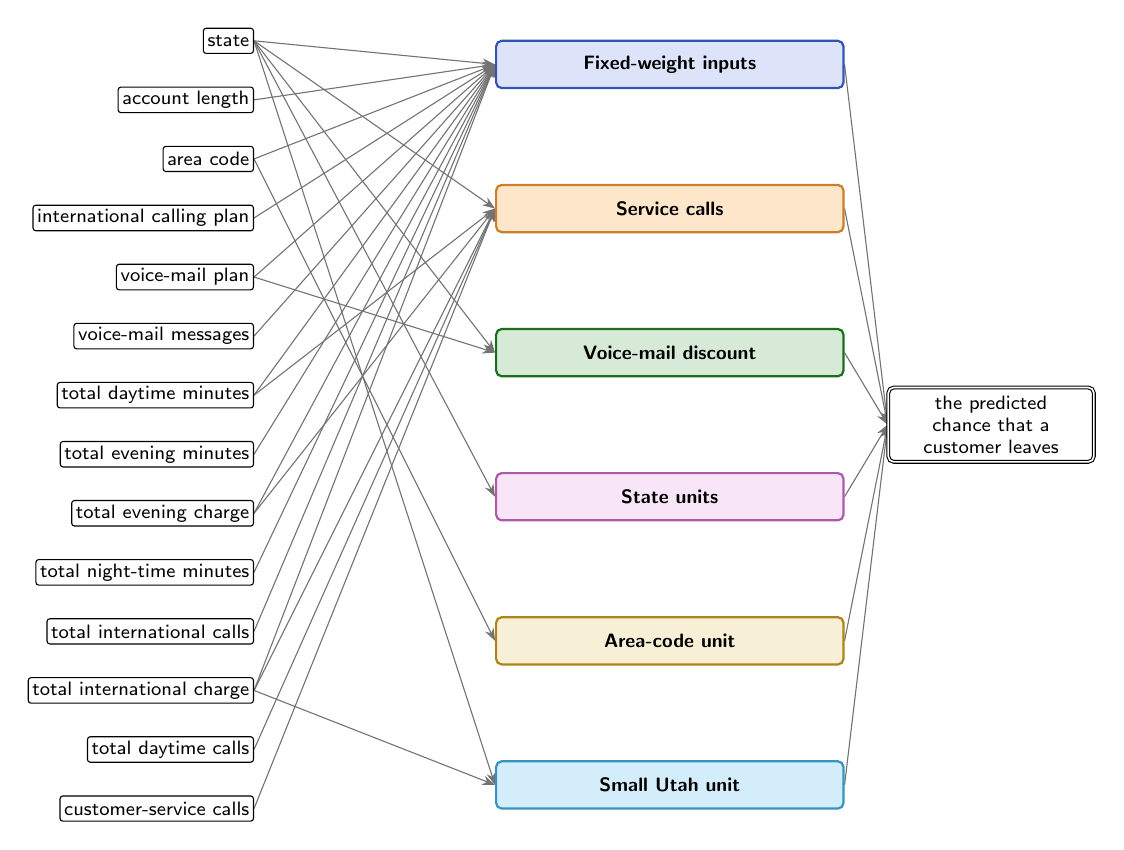
\begin{tikzpicture}[
  font=\sffamily\scriptsize, >={Stealth[length=1.6mm]},
  inp/.style={draw, rounded corners=1pt, fill=white, inner sep=1.5pt, minimum height=3.2mm, anchor=east},
  abox/.style={draw, thick, rounded corners=2pt, align=center, inner sep=3pt, minimum height=6mm, text width=42mm},
  outp/.style={draw, double, rounded corners=2pt, fill=white, align=center, inner sep=3pt, text width=24mm},
  agg/.style={draw=black!55},
]
\node[inp] (i0) at (0,4.875) {state};
\node[inp] (i1) at (0,4.125) {account length};
\node[inp] (i2) at (0,3.375) {area code};
\node[inp] (i3) at (0,2.625) {international calling plan};
\node[inp] (i4) at (0,1.875) {voice-mail plan};
\node[inp] (i5) at (0,1.125) {voice-mail messages};
\node[inp] (i6) at (0,0.375) {total daytime minutes};
\node[inp] (i7) at (0,-0.375) {total evening minutes};
\node[inp] (i8) at (0,-1.125) {total evening charge};
\node[inp] (i9) at (0,-1.875) {total night-time minutes};
\node[inp] (i10) at (0,-2.625) {total international calls};
\node[inp] (i11) at (0,-3.375) {total international charge};
\node[inp] (i12) at (0,-4.125) {total daytime calls};
\node[inp] (i13) at (0,-4.875) {customer-service calls};
\node[abox, fill=RoyalBlue!18, draw=RoyalBlue!80!black] (b0) at (5.28,4.575) {\textbf{Fixed-weight inputs}};
\node[abox, fill=BurntOrange!18, draw=BurntOrange!80!black] (b1) at (5.28,2.745) {\textbf{Service calls}};
\node[abox, fill=ForestGreen!18, draw=ForestGreen!80!black] (b2) at (5.28,0.915) {\textbf{Voice-mail discount}};
\node[abox, fill=Orchid!18, draw=Orchid!80!black] (b3) at (5.28,-0.915) {\textbf{State units}};
\node[abox, fill=Goldenrod!18, draw=Goldenrod!80!black] (b4) at (5.28,-2.745) {\textbf{Area-code unit}};
\node[abox, fill=Cerulean!18, draw=Cerulean!80!black] (b5) at (5.28,-4.575) {\textbf{Small Utah unit}};
\node[outp] (out) at (9.36,0) {the predicted chance that a customer leaves};
\begin{scope}[on background layer]
\draw[->, agg, thin] (i0.east) -- (b0.west);
\draw[->, agg, thin] (i1.east) -- (b0.west);
\draw[->, agg, thin] (i2.east) -- (b0.west);
\draw[->, agg, thin] (i3.east) -- (b0.west);
\draw[->, agg, thin] (i4.east) -- (b0.west);
\draw[->, agg, thin] (i5.east) -- (b0.west);
\draw[->, agg, thin] (i6.east) -- (b0.west);
\draw[->, agg, thin] (i7.east) -- (b0.west);
\draw[->, agg, thin] (i8.east) -- (b0.west);
\draw[->, agg, thin] (i9.east) -- (b0.west);
\draw[->, agg, thin] (i10.east) -- (b0.west);
\draw[->, agg, thin] (i11.east) -- (b0.west);
\draw[->, agg] (b0.east) -- (out.west);
\draw[->, agg, thin] (i0.east) -- (b1.west);
\draw[->, agg, thin] (i6.east) -- (b1.west);
\draw[->, agg, thin] (i12.east) -- (b1.west);
\draw[->, agg, thin] (i8.east) -- (b1.west);
\draw[->, agg, thin] (i11.east) -- (b1.west);
\draw[->, agg, thin] (i13.east) -- (b1.west);
\draw[->, agg] (b1.east) -- (out.west);
\draw[->, agg, thin] (i0.east) -- (b2.west);
\draw[->, agg, thin] (i4.east) -- (b2.west);
\draw[->, agg] (b2.east) -- (out.west);
\draw[->, agg, thin] (i0.east) -- (b3.west);
\draw[->, agg] (b3.east) -- (out.west);
\draw[->, agg, thin] (i2.east) -- (b4.west);
\draw[->, agg] (b4.east) -- (out.west);
\draw[->, agg, thin] (i0.east) -- (b5.west);
\draw[->, agg, thin] (i11.east) -- (b5.west);
\draw[->, agg] (b5.east) -- (out.west);
\end{scope}
\end{tikzpicture}}}%
\caption{The whole model: what feeds it, one level down.}
\label{fig:churn100s2c2:parts-ann97}
\end{figure}
\begin{figure}[H]\centering
\resizebox{\ifdim\width>\linewidth\linewidth\else\width\fi}{!}{%
\definecolor{netup}{HTML}{D95F02}\definecolor{netdown}{HTML}{1B9E77}\definecolor{netmixed}{HTML}{7F7F7F}%
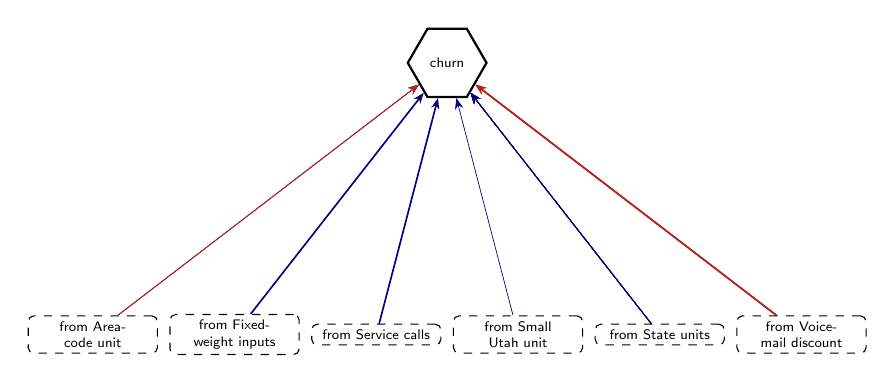
\begin{tikzpicture}[
  font=\sffamily\scriptsize, >={Stealth[length=1.4mm]},
  inp/.style={draw, circle, fill=white, minimum size=3.2mm, inner sep=0pt},
  hid/.style={draw, circle, fill=white, minimum size=5.2mm, inner sep=0.5pt, font=\sffamily\tiny},
  exitbox/.style={draw, thick, rectangle, fill=white, align=center, text width=17mm, minimum height=5mm, inner sep=1.5pt, font=\sffamily\tiny},
  sumbox/.style={draw, thick, dashed, rectangle, fill=white, align=center, text width=17mm, minimum height=5mm, inner sep=1.5pt, font=\sffamily\tiny},
  outp/.style={draw, thick, regular polygon, regular polygon sides=6, fill=white, minimum size=10mm, inner sep=0pt, font=\sffamily\tiny, align=center},
  stub/.style={draw, dashed, rounded corners=2pt, fill=white, align=center, inner sep=2pt, font=\sffamily\tiny, text width=15mm},
  inlab/.style={font=\sffamily\tiny, align=center, text width=15mm, inner sep=1pt, fill=white, fill opacity=0.8, text opacity=1},
  wpos/.style={draw=NavyBlue}, wneg/.style={draw=BrickRed}, wagg/.style={draw=black!45, line width=1.2pt},
  wmix/.style={draw=Plum},
]
\node[outp] (n0) at (5.4,3.45) {churn};
\node[stub] (nfromxxAreamcodexunit) at (0.9,0.0) {from Area-code unit};
\node[stub] (nfromxxSmallxUtahxunit) at (6.3,0.0) {from Small Utah unit};
\node[stub] (nfromxxVoicemmailxdiscount) at (9.9,0.0) {from Voice-mail discount};
\node[stub] (nfromxxStatexunits) at (8.1,0.0) {from State units};
\node[stub] (nfromxxFixedmweightxinputs) at (2.7,0.0) {from Fixed-weight inputs};
\node[stub] (nfromxxServicexcalls) at (4.5,0.0) {from Service calls};
\begin{scope}[on background layer]
\draw[->, wpos, line width=0.27pt] (nfromxxAreamcodexunit) -- (n0);
\draw[->, wpos, line width=0.25pt] (nfromxxSmallxUtahxunit) -- (n0);
\draw[->, wneg, line width=0.56pt] (nfromxxVoicemmailxdiscount) -- (n0);
\draw[->, wneg, line width=0.60pt] (nfromxxVoicemmailxdiscount) -- (n0);
\draw[->, wneg, line width=0.25pt] (nfromxxStatexunits) -- (n0);
\draw[->, wneg, line width=0.25pt] (nfromxxStatexunits) -- (n0);
\draw[->, wneg, line width=0.25pt] (nfromxxStatexunits) -- (n0);
\draw[->, wpos, line width=0.29pt] (nfromxxStatexunits) -- (n0);
\draw[->, wpos, line width=0.27pt] (nfromxxStatexunits) -- (n0);
\draw[->, wpos, line width=0.27pt] (nfromxxStatexunits) -- (n0);
\draw[->, wneg, line width=0.34pt] (nfromxxAreamcodexunit) -- (n0);
\draw[->, wpos, line width=0.27pt] (nfromxxStatexunits) -- (n0);
\draw[->, wpos, line width=0.27pt] (nfromxxStatexunits) -- (n0);
\draw[->, wpos, line width=0.60pt] (nfromxxFixedmweightxinputs) -- (n0);
\draw[->, wpos, line width=0.60pt] (nfromxxServicexcalls) -- (n0);
\end{scope}
\end{tikzpicture}}%
\caption{The whole model: its units and every connection into them. Blue: positive weight (raises the score); red: negative weight (lowers it); thicker: larger weight. Orange outline and up arrow: raises the final prediction; teal and down arrow: lowers it; grey and double arrow: depends.}
\label{fig:churn100s2c2:units-ann97}
\end{figure}
\paragraph{Hypothesis.} The model adds up six parts into one score: fixed-weight inputs, service calls, a voice-mail discount, state units, an area-code unit and a small Utah unit.\,{\scriptsize\textcolor{NavyBlue}{[C051]}}
\paragraph{Evidence.} It is made up of these six parts (each explained below); the score is their sum, which was checked on all 4000 training customers.\,{\scriptsize\textcolor{NavyBlue}{[C051]}} Changing one input at a time across the whole model, an international plan takes a typical customer's chance of leaving from about 1\% to about 14\%, and a voice-mail plan lowers it to under 1\%.\,{\scriptsize\textcolor{NavyBlue}{[C001, C010]}} In Washington the chance is about 9\%, against about 1\% in West Virginia.\,{\scriptsize\textcolor{NavyBlue}{[C003]}} More customer-service calls raise it slowly at first, then faster, from about 1\% at 0 calls to about 2\% at 3 calls.\,{\scriptsize\textcolor{NavyBlue}{[C011]}} The model ignores the daytime charge, evening calls, international minutes, night-time calls and the night-time charge.\,{\scriptsize\textcolor{NavyBlue}{[C046, C047, C048, C049, C050]}}
\par\noindent{\small Evidence plots: Figure~\ref{fig:churn100s2c2:plot-ann97-0}, Figure~\ref{fig:churn100s2c2:plot-ann97-1}.\par}
\begin{figure}[H]\centering
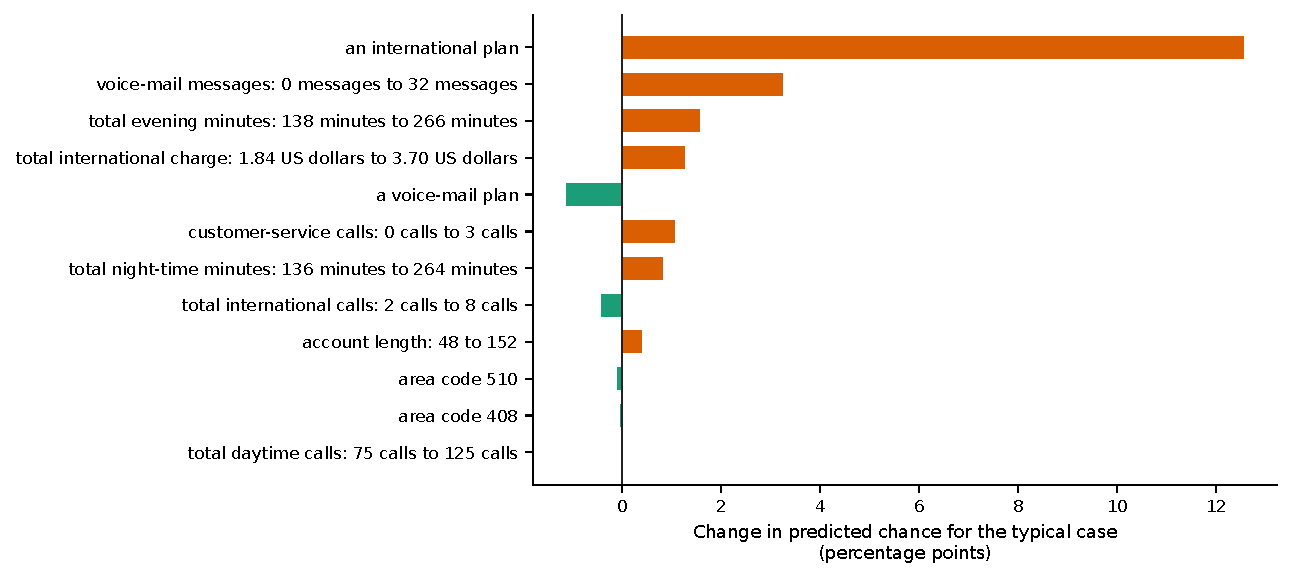
\includegraphics[width=\linewidth,height=0.88\textheight,keepaspectratio]{figures/churn100-s2-c2/ann_97-effects.pdf}
\caption{The whole model: Each input's change in the predicted value for the typical case across the whole model, largest first (orange: raises it, teal: lowers it).}
\label{fig:churn100s2c2:plot-ann97-0}
\end{figure}
\begin{figure}[H]\centering
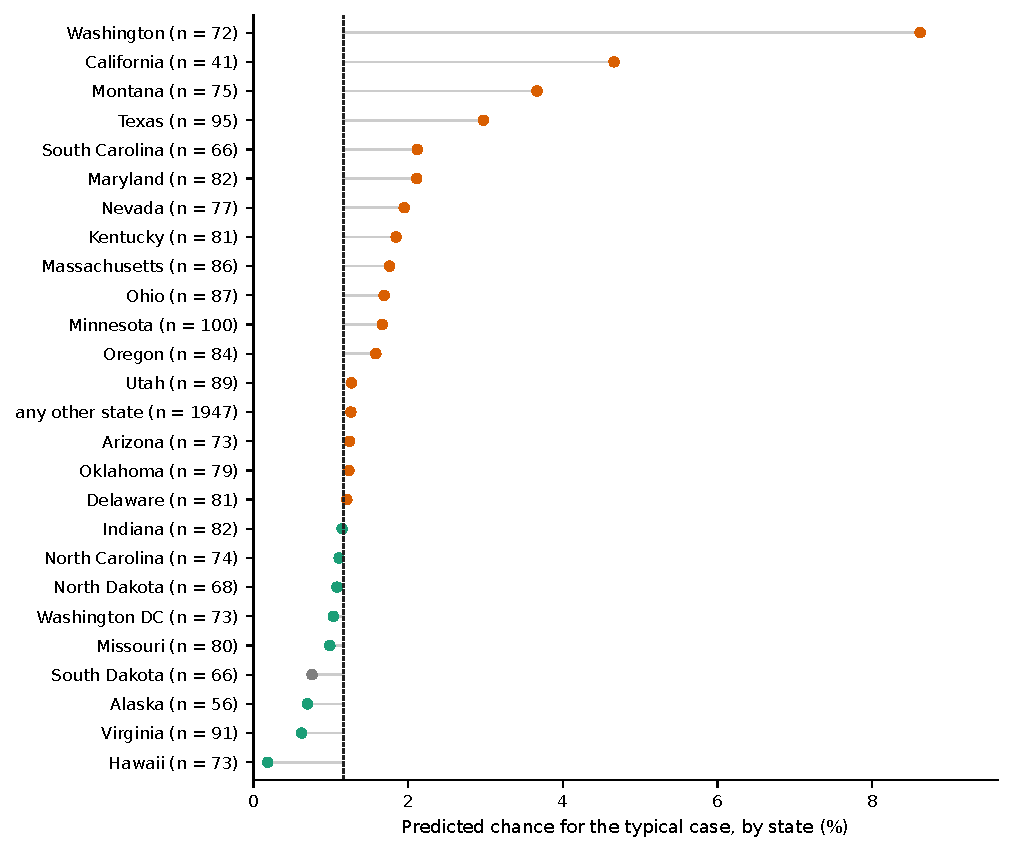
\includegraphics[width=\linewidth,height=0.88\textheight,keepaspectratio]{figures/churn100-s2-c2/ann_97-levels-state.pdf}
\caption{The whole model: Every level of state the model reads: the predicted value for the typical case at that level (dashed: the reference level); n = training customers; grey: few customers or not supported.}
\label{fig:churn100s2c2:plot-ann97-1}
\end{figure}
\par\smallskip\noindent{\small \textbf{Dive deeper:} Fixed-weight inputs (\ref{rd:ann89}); Service calls (\ref{rd:ann96}); Voice-mail discount (\ref{rd:ann92}); State units (\ref{rd:ann95}); Area-code unit (\ref{rd:ann94}); Small Utah unit (\ref{rd:ann93}). Technical detail: \ref{tech:ann97}.\par}
\subsubsection{Fixed-weight inputs}\label{rd:ann89}
\noindent{\footnotesize Part of: The whole model (\ref{rd:ann97}).\par}
\noindent{\small Figure~\ref{fig:churn100s2c2:parts-ann89} shows what feeds this part; Figure~\ref{fig:churn100s2c2:units-ann89} its units and every connection into them (dashed boxes: connections from or to other parts, drawn in their own sections).\par}
\begin{figure}[H]\centering
\resizebox{!}{\ifdim\height>0.5\textheight 0.5\textheight\else\height\fi}{%
\resizebox{\ifdim\width>\linewidth\linewidth\else\width\fi}{!}{%
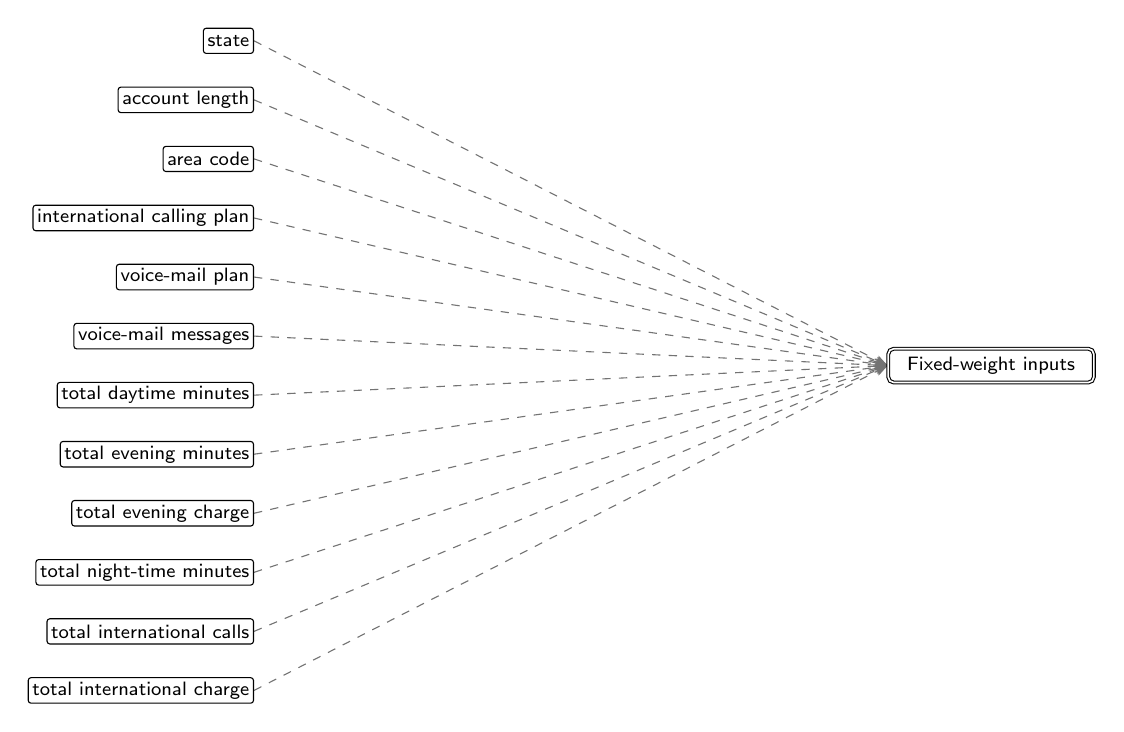
\begin{tikzpicture}[
  font=\sffamily\scriptsize, >={Stealth[length=1.6mm]},
  inp/.style={draw, rounded corners=1pt, fill=white, inner sep=1.5pt, minimum height=3.2mm, anchor=east},
  abox/.style={draw, thick, rounded corners=2pt, align=center, inner sep=3pt, minimum height=6mm, text width=42mm},
  outp/.style={draw, double, rounded corners=2pt, fill=white, align=center, inner sep=3pt, text width=24mm},
  agg/.style={draw=black!55},
]
\node[inp] (i0) at (0,4.125) {state};
\node[inp] (i1) at (0,3.375) {account length};
\node[inp] (i2) at (0,2.625) {area code};
\node[inp] (i3) at (0,1.875) {international calling plan};
\node[inp] (i4) at (0,1.125) {voice-mail plan};
\node[inp] (i5) at (0,0.375) {voice-mail messages};
\node[inp] (i6) at (0,-0.375) {total daytime minutes};
\node[inp] (i7) at (0,-1.125) {total evening minutes};
\node[inp] (i8) at (0,-1.875) {total evening charge};
\node[inp] (i9) at (0,-2.625) {total night-time minutes};
\node[inp] (i10) at (0,-3.375) {total international calls};
\node[inp] (i11) at (0,-4.125) {total international charge};
\node[outp] (out) at (9.36,0) {Fixed-weight inputs};
\begin{scope}[on background layer]
\draw[->, agg, thin, dashed] (i0.east) -- (out.west);
\draw[->, agg, thin, dashed] (i1.east) -- (out.west);
\draw[->, agg, thin, dashed] (i2.east) -- (out.west);
\draw[->, agg, thin, dashed] (i3.east) -- (out.west);
\draw[->, agg, thin, dashed] (i4.east) -- (out.west);
\draw[->, agg, thin, dashed] (i5.east) -- (out.west);
\draw[->, agg, thin, dashed] (i6.east) -- (out.west);
\draw[->, agg, thin, dashed] (i7.east) -- (out.west);
\draw[->, agg, thin, dashed] (i8.east) -- (out.west);
\draw[->, agg, thin, dashed] (i9.east) -- (out.west);
\draw[->, agg, thin, dashed] (i10.east) -- (out.west);
\draw[->, agg, thin, dashed] (i11.east) -- (out.west);
\end{scope}
\end{tikzpicture}}}%
\caption{Fixed-weight inputs: what feeds it, one level down.}
\label{fig:churn100s2c2:parts-ann89}
\end{figure}
\begin{figure}[H]\centering
\resizebox{\ifdim\width>\linewidth\linewidth\else\width\fi}{!}{%
\definecolor{netup}{HTML}{D95F02}\definecolor{netdown}{HTML}{1B9E77}\definecolor{netmixed}{HTML}{7F7F7F}%
\begin{tikzpicture}[
  font=\sffamily\scriptsize, >={Stealth[length=1.4mm]},
  inp/.style={draw, circle, fill=white, minimum size=3.2mm, inner sep=0pt},
  hid/.style={draw, circle, fill=white, minimum size=5.2mm, inner sep=0.5pt, font=\sffamily\tiny},
  exitbox/.style={draw, thick, rectangle, fill=white, align=center, text width=17mm, minimum height=5mm, inner sep=1.5pt, font=\sffamily\tiny},
  sumbox/.style={draw, thick, dashed, rectangle, fill=white, align=center, text width=17mm, minimum height=5mm, inner sep=1.5pt, font=\sffamily\tiny},
  outp/.style={draw, thick, regular polygon, regular polygon sides=6, fill=white, minimum size=10mm, inner sep=0pt, font=\sffamily\tiny, align=center},
  stub/.style={draw, dashed, rounded corners=2pt, fill=white, align=center, inner sep=2pt, font=\sffamily\tiny, text width=15mm},
  inlab/.style={font=\sffamily\tiny, align=center, text width=15mm, inner sep=1pt, fill=white, fill opacity=0.8, text opacity=1},
  wpos/.style={draw=NavyBlue}, wneg/.style={draw=BrickRed}, wagg/.style={draw=black!45, line width=1.2pt},
  wmix/.style={draw=Plum},
]
\node[exitbox] (nidentityxlin) at (5.85,1.9) {Fixed-weight inputs $\uparrow$};
\node[inp, draw=netmixed, very thick] (ngrpxxstate) at (4.5,0.0) {};
\path (ngrpxxstate.south) node[inlab, anchor=north] (labngrpxxstate) {state (26 of 51 used) $\updownarrow$};
\node[inp, draw=netup, very thick] (ninxxaccountxlength) at (1.8,-1.05) {};
\path (ninxxaccountxlength.south) node[inlab, anchor=north] (labninxxaccountxlength) {account length $\uparrow$};
\node[inp, draw=netdown, very thick] (ninxxareaxcodex510) at (3.6,-1.05) {};
\path (ninxxareaxcodex510.south) node[inlab, anchor=north] (labninxxareaxcodex510) {area code 510 $\downarrow$};
\node[inp, draw=netup, very thick] (ninxxinternationalxplan) at (2.7,0.0) {};
\path (ninxxinternationalxplan.south) node[inlab, anchor=north] (labninxxinternationalxplan) {an international plan $\uparrow$};
\node[inp, draw=netup, very thick] (ninxxnumberxvmailxmessages) at (10.8,-1.05) {};
\path (ninxxnumberxvmailxmessages.south) node[inlab, anchor=north] (labninxxnumberxvmailxmessages) {voice-mail messages $\uparrow$};
\node[inp, draw=netup, very thick] (ninxxtotalxevexminutes) at (7.2,-1.05) {};
\path (ninxxtotalxevexminutes.south) node[inlab, anchor=north] (labninxxtotalxevexminutes) {total evening minutes $\uparrow$};
\node[inp, draw=netup, very thick] (ninxxtotalxnightxminutes) at (9.9,0.0) {};
\path (ninxxtotalxnightxminutes.south) node[inlab, anchor=north] (labninxxtotalxnightxminutes) {total night-time minutes $\uparrow$};
\node[inp, draw=netdown, very thick] (ninxxtotalxintlxcalls) at (8.1,0.0) {};
\path (ninxxtotalxintlxcalls.south) node[inlab, anchor=north] (labninxxtotalxintlxcalls) {total international calls $\downarrow$};
\node[inp, draw=netup, very thick] (ninxxtotalxintlxcharge) at (9.0,-1.05) {};
\path (ninxxtotalxintlxcharge.south) node[inlab, anchor=north] (labninxxtotalxintlxcharge) {total international charge $\uparrow$};
\node[inp, draw=netup, very thick] (ninxxtotalxevexcharge) at (6.3,0.0) {};
\path (ninxxtotalxevexcharge.south) node[inlab, anchor=north] (labninxxtotalxevexcharge) {total evening charge $\uparrow$};
\node[inp, draw=netup, very thick] (ninxxtotalxdayxminutes) at (5.4,-1.05) {};
\path (ninxxtotalxdayxminutes.south) node[inlab, anchor=north] (labninxxtotalxdayxminutes) {total daytime minutes $\uparrow$};
\node[inp, draw=netdown, very thick] (ninxxvoicexmailxplan) at (0.9,0.0) {};
\path (ninxxvoicexmailxplan.south) node[inlab, anchor=north] (labninxxvoicexmailxplan) {a voice-mail plan $\downarrow$};
\node[stub] (ntoxxthexmodelxoutput) at (5.85,3.45) {to the model output};
\begin{scope}[on background layer]
\node[fit=(nidentityxlin) , inner sep=8pt, rounded corners=5pt, fill=BurntOrange!10, draw=BurntOrange!45] (clu0) {};
\draw[->, wpos, line width=0.29pt] (ninxxaccountxlength) -- (nidentityxlin);
\draw[->, wneg, line width=0.26pt] (ninxxareaxcodex510) -- (nidentityxlin);
\draw[->, wpos, line width=0.52pt] (ninxxinternationalxplan) -- (nidentityxlin);
\draw[->, wpos, line width=0.45pt] (ninxxnumberxvmailxmessages) -- (nidentityxlin);
\draw[->, wpos, line width=0.42pt] (ninxxtotalxevexminutes) -- (nidentityxlin);
\draw[->, wpos, line width=0.35pt] (ninxxtotalxnightxminutes) -- (nidentityxlin);
\draw[->, wneg, line width=0.31pt] (ninxxtotalxintlxcalls) -- (nidentityxlin);
\draw[->, wpos, line width=0.49pt] (ninxxtotalxintlxcharge) -- (nidentityxlin);
\draw[->, wpos, line width=0.37pt] (ninxxtotalxevexcharge) -- (nidentityxlin);
\draw[->, wpos, line width=0.90pt] (ninxxtotalxdayxminutes) -- (nidentityxlin);
\draw[->, wneg, line width=0.56pt] (ninxxvoicexmailxplan) -- (nidentityxlin);
\draw[->, wpos, line width=0.60pt] (nidentityxlin) -- (ntoxxthexmodelxoutput);
\draw[->, wmix, line width=0.34pt] (ngrpxxstate) -- node[pos=0.8, sloped, above, font=\sffamily\tiny, inner sep=1pt, fill=white, fill opacity=0.8, text opacity=1] {22 edges, -0.26 to +0.18} (nidentityxlin);
\end{scope}
\node[font=\sffamily\scriptsize\bfseries, text=BurntOrange!55!black, anchor=south west, inner sep=1pt, fill=white, fill opacity=0.85, text opacity=1] at (clu0.north west) {Fixed-weight inputs};
\end{tikzpicture}}%
\caption{Fixed-weight inputs: its units and every connection into them. Blue: positive weight (raises the score); red: negative weight (lowers it); thicker: larger weight. Orange outline and up arrow: raises the final prediction; teal and down arrow: lowers it; grey and double arrow: depends.}
\label{fig:churn100s2c2:units-ann89}
\end{figure}
\paragraph{Hypothesis.} This part adds up most inputs with fixed weights: daytime minutes, an international plan and voice-mail messages raise the chance of leaving, steadily for the minutes and messages, and a voice-mail plan lowers it.\,{\scriptsize\textcolor{NavyBlue}{[C053, C052, C056, C061]}}
\paragraph{Evidence.} Through it, daytime minutes take a typical customer steadily from under 1\% at 112 to about 11\% at 249 minutes, and an international plan from about 1\% to about 14\%; a voice-mail plan lowers the chance to under 1\%.\,{\scriptsize\textcolor{NavyBlue}{[C053, C052, C061]}} Through it, the state moves the chance from about 1\% in West Virginia to about 5\% in Washington and in California, and to under 1\% in Hawaii (41 to 122 training customers per state).\,{\scriptsize\textcolor{NavyBlue}{[C054, C055, C062]}} Its formula reproduces the part exactly on all 4000 training customers.\,{\scriptsize\textcolor{NavyBlue}{[C085]}}
\par\noindent{\small Evidence plots: Figure~\ref{fig:churn100s2c2:plot-ann89-0}, Figure~\ref{fig:churn100s2c2:plot-ann89-1}, Figure~\ref{fig:churn100s2c2:plot-ann89-2}, Figure~\ref{fig:churn100s2c2:plot-ann89-3}.\par}
\begin{figure}[H]\centering
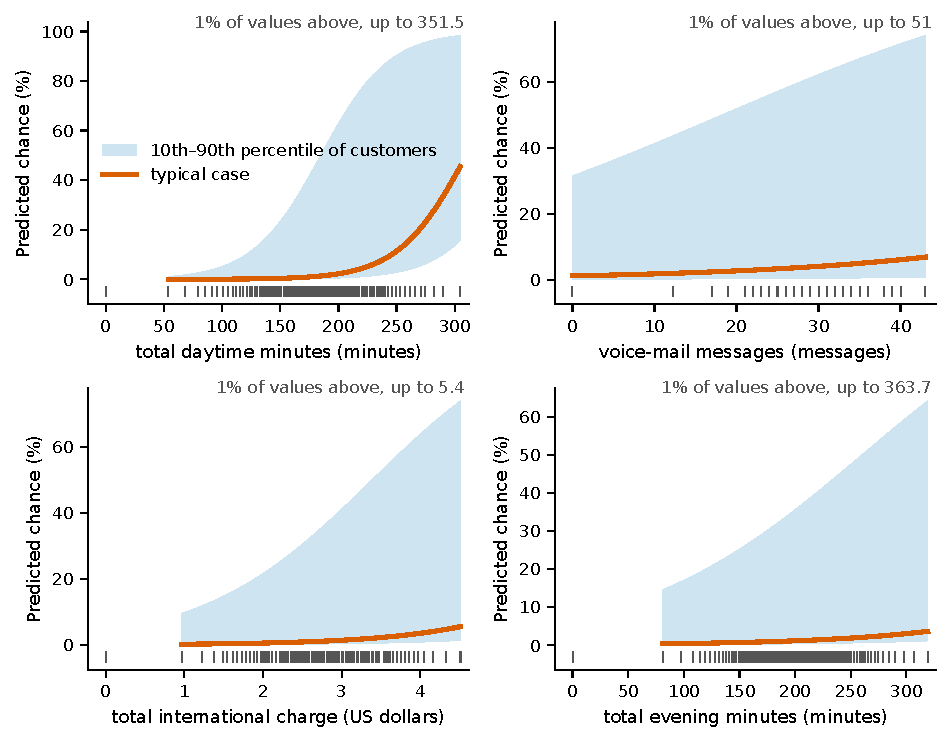
\includegraphics[width=\linewidth,height=0.88\textheight,keepaspectratio]{figures/churn100-s2-c2/ann_89-response.pdf}
\caption{Fixed-weight inputs: Response curves through this part: the typical case (bold), the 10th to 90th percentile of individual customers (band), the fold or step point (dashed) with its spread across them (grey), and the observed values (ticks).}
\label{fig:churn100s2c2:plot-ann89-0}
\end{figure}
\begin{figure}[H]\centering
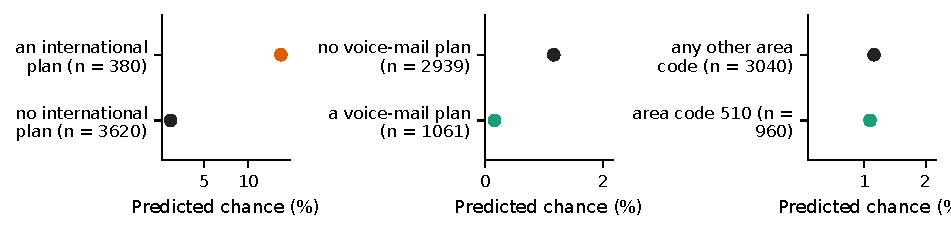
\includegraphics[width=\linewidth,height=0.88\textheight,keepaspectratio]{figures/churn100-s2-c2/ann_89-categories-small.pdf}
\caption{Fixed-weight inputs: The predicted value for the typical case at each level, through this part (n = training customers; grey: fewer than 20).}
\label{fig:churn100s2c2:plot-ann89-1}
\end{figure}
\begin{figure}[H]\centering
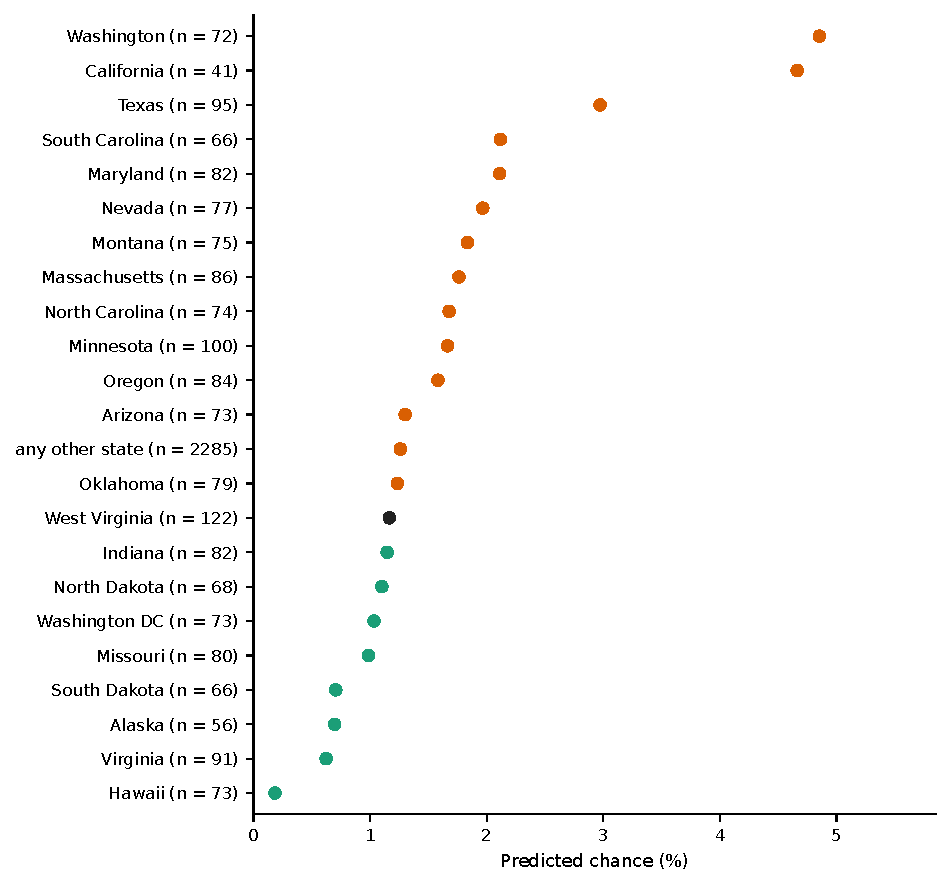
\includegraphics[width=\linewidth,height=0.88\textheight,keepaspectratio]{figures/churn100-s2-c2/ann_89-categories-C054.pdf}
\caption{Fixed-weight inputs: The predicted value for the typical case at each level, through this part (n = training customers; grey: fewer than 20).}
\label{fig:churn100s2c2:plot-ann89-2}
\end{figure}
\begin{figure}[H]\centering
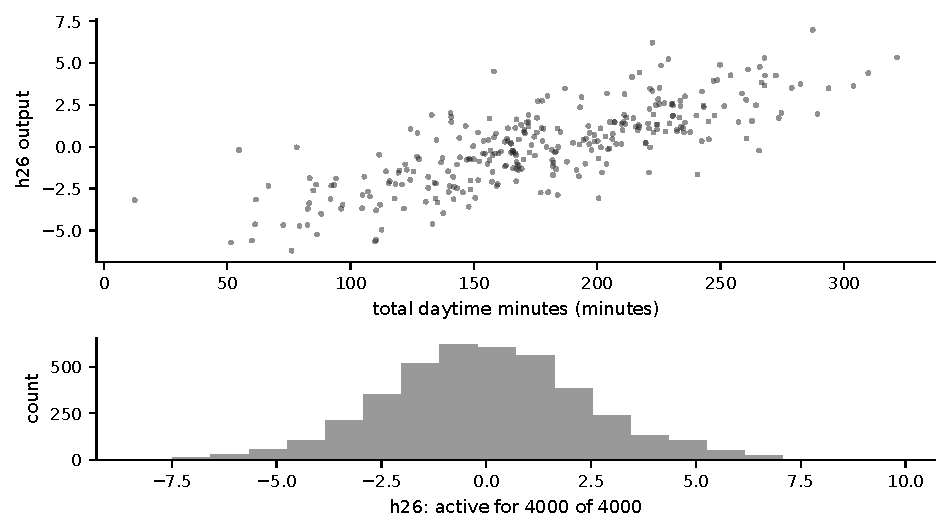
\includegraphics[width=\linewidth,height=0.88\textheight,keepaspectratio]{figures/churn100-s2-c2/ann_89-units.pdf}
\caption{Fixed-weight inputs: This part's hidden units: each unit's output against its main numeric input (top) and how often it is active (bottom).}
\label{fig:churn100s2c2:plot-ann89-3}
\end{figure}
\par\smallskip\noindent{\small Technical detail: \ref{tech:ann89}.\par}
\subsubsection{Service calls}\label{rd:ann96}
\noindent{\footnotesize Part of: The whole model (\ref{rd:ann97}).\par}
\noindent{\small Figure~\ref{fig:churn100s2c2:parts-ann96} shows what feeds this part; Figure~\ref{fig:churn100s2c2:units-ann96} its units and every connection into them (dashed boxes: connections from or to other parts, drawn in their own sections).\par}
\begin{figure}[H]\centering
\resizebox{!}{\ifdim\height>0.5\textheight 0.5\textheight\else\height\fi}{%
\resizebox{\ifdim\width>\linewidth\linewidth\else\width\fi}{!}{%
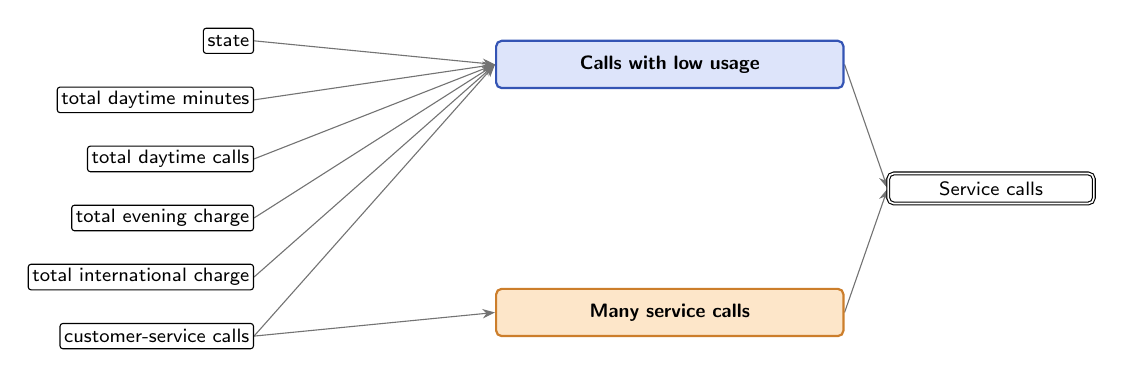
\begin{tikzpicture}[
  font=\sffamily\scriptsize, >={Stealth[length=1.6mm]},
  inp/.style={draw, rounded corners=1pt, fill=white, inner sep=1.5pt, minimum height=3.2mm, anchor=east},
  abox/.style={draw, thick, rounded corners=2pt, align=center, inner sep=3pt, minimum height=6mm, text width=42mm},
  outp/.style={draw, double, rounded corners=2pt, fill=white, align=center, inner sep=3pt, text width=24mm},
  agg/.style={draw=black!55},
]
\node[inp] (i0) at (0,1.875) {state};
\node[inp] (i1) at (0,1.125) {total daytime minutes};
\node[inp] (i2) at (0,0.375) {total daytime calls};
\node[inp] (i3) at (0,-0.375) {total evening charge};
\node[inp] (i4) at (0,-1.125) {total international charge};
\node[inp] (i5) at (0,-1.875) {customer-service calls};
\node[abox, fill=RoyalBlue!18, draw=RoyalBlue!80!black] (b0) at (5.28,1.575) {\textbf{Calls with low usage}};
\node[abox, fill=BurntOrange!18, draw=BurntOrange!80!black] (b1) at (5.28,-1.575) {\textbf{Many service calls}};
\node[outp] (out) at (9.36,0) {Service calls};
\begin{scope}[on background layer]
\draw[->, agg, thin] (i0.east) -- (b0.west);
\draw[->, agg, thin] (i1.east) -- (b0.west);
\draw[->, agg, thin] (i2.east) -- (b0.west);
\draw[->, agg, thin] (i3.east) -- (b0.west);
\draw[->, agg, thin] (i4.east) -- (b0.west);
\draw[->, agg, thin] (i5.east) -- (b0.west);
\draw[->, agg] (b0.east) -- (out.west);
\draw[->, agg, thin] (i5.east) -- (b1.west);
\draw[->, agg] (b1.east) -- (out.west);
\end{scope}
\end{tikzpicture}}}%
\caption{Service calls: what feeds it, one level down.}
\label{fig:churn100s2c2:parts-ann96}
\end{figure}
\begin{figure}[H]\centering
\resizebox{\ifdim\width>\linewidth\linewidth\else\width\fi}{!}{%
\definecolor{netup}{HTML}{D95F02}\definecolor{netdown}{HTML}{1B9E77}\definecolor{netmixed}{HTML}{7F7F7F}%
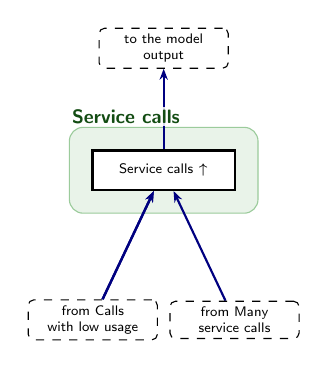
\begin{tikzpicture}[
  font=\sffamily\scriptsize, >={Stealth[length=1.4mm]},
  inp/.style={draw, circle, fill=white, minimum size=3.2mm, inner sep=0pt},
  hid/.style={draw, circle, fill=white, minimum size=5.2mm, inner sep=0.5pt, font=\sffamily\tiny},
  exitbox/.style={draw, thick, rectangle, fill=white, align=center, text width=17mm, minimum height=5mm, inner sep=1.5pt, font=\sffamily\tiny},
  sumbox/.style={draw, thick, dashed, rectangle, fill=white, align=center, text width=17mm, minimum height=5mm, inner sep=1.5pt, font=\sffamily\tiny},
  outp/.style={draw, thick, regular polygon, regular polygon sides=6, fill=white, minimum size=10mm, inner sep=0pt, font=\sffamily\tiny, align=center},
  stub/.style={draw, dashed, rounded corners=2pt, fill=white, align=center, inner sep=2pt, font=\sffamily\tiny, text width=15mm},
  inlab/.style={font=\sffamily\tiny, align=center, text width=15mm, inner sep=1pt, fill=white, fill opacity=0.8, text opacity=1},
  wpos/.style={draw=NavyBlue}, wneg/.style={draw=BrickRed}, wagg/.style={draw=black!45, line width=1.2pt},
  wmix/.style={draw=Plum},
]
\node[exitbox] (nidentityxsvc) at (1.8,1.9) {Service calls $\uparrow$};
\node[stub] (nfromxxCallsxwithxlowxusage) at (0.9,0.0) {from Calls with low usage};
\node[stub] (nfromxxManyxservicexcalls) at (2.7,0.0) {from Many service calls};
\node[stub] (ntoxxthexmodelxoutput) at (1.8,3.45) {to the model output};
\begin{scope}[on background layer]
\node[fit=(nidentityxsvc) , inner sep=8pt, rounded corners=5pt, fill=ForestGreen!10, draw=ForestGreen!45] (clu0) {};
\draw[->, wpos, line width=0.80pt] (nfromxxCallsxwithxlowxusage) -- (nidentityxsvc);
\draw[->, wpos, line width=0.88pt] (nfromxxCallsxwithxlowxusage) -- (nidentityxsvc);
\draw[->, wpos, line width=0.78pt] (nfromxxManyxservicexcalls) -- (nidentityxsvc);
\draw[->, wpos, line width=0.60pt] (nidentityxsvc) -- (ntoxxthexmodelxoutput);
\end{scope}
\node[font=\sffamily\scriptsize\bfseries, text=ForestGreen!55!black, anchor=south west, inner sep=1pt, fill=white, fill opacity=0.85, text opacity=1] at (clu0.north west) {Service calls};
\end{tikzpicture}}%
\caption{Service calls: its units and every connection into them. Blue: positive weight (raises the score); red: negative weight (lowers it); thicker: larger weight. Orange outline and up arrow: raises the final prediction; teal and down arrow: lowers it; grey and double arrow: depends.}
\label{fig:churn100s2c2:units-ann96}
\end{figure}
\paragraph{Hypothesis.} This part raises the chance of leaving with calls to customer service, from 4 calls upwards, slowly at first, then faster, and more so for customers with low daytime use, in an uneven way; it adds up two parts.\,{\scriptsize\textcolor{NavyBlue}{[C103, C099, C098]}}
\paragraph{Evidence.} It is made of two parts that are added: calls with low usage, and many service calls.\,{\scriptsize\textcolor{NavyBlue}{[C103]}} Through it, daytime minutes lower the chance only while they stay below about 166 minutes (between 145 and 213 minutes for different customers), in an uneven way: for a typical such customer, from about 28\% at 91 minutes to about 1\% at 352 minutes.\,{\scriptsize\textcolor{NavyBlue}{[C098]}} Customer-service calls add to it from 4 calls upwards, slowly at first, then faster: for a typical such customer, from about 3\% at 0 calls to about 8\% at 4 calls.\,{\scriptsize\textcolor{NavyBlue}{[C099]}} With an evening charge above 17.12 US dollars, the chance is lowest at about 148 minutes of daytime use and higher either side: from about 1\% at 112 minutes to about 13\% at 249 minutes, against about 2\% to about 9\% at or below that charge.\,{\scriptsize\textcolor{NavyBlue}{[C095]}}
\par\noindent{\small Evidence plots: Figure~\ref{fig:churn100s2c2:plot-ann96-0}, Figure~\ref{fig:churn100s2c2:plot-ann96-1}, Figure~\ref{fig:churn100s2c2:plot-ann96-2}, Figure~\ref{fig:churn100s2c2:plot-ann96-3}, Figure~\ref{fig:churn100s2c2:plot-ann96-4}, Figure~\ref{fig:churn100s2c2:plot-ann96-5}, Figure~\ref{fig:churn100s2c2:plot-ann96-6}, Figure~\ref{fig:churn100s2c2:plot-ann96-7}.\par}
\par\noindent{\small Figure~\ref{fig:churn100s2c2:plot-ann96-6} shows this part's own output, unit h27: over its two main inputs, with the line where it switches on.\par}
\begin{figure}[H]\centering
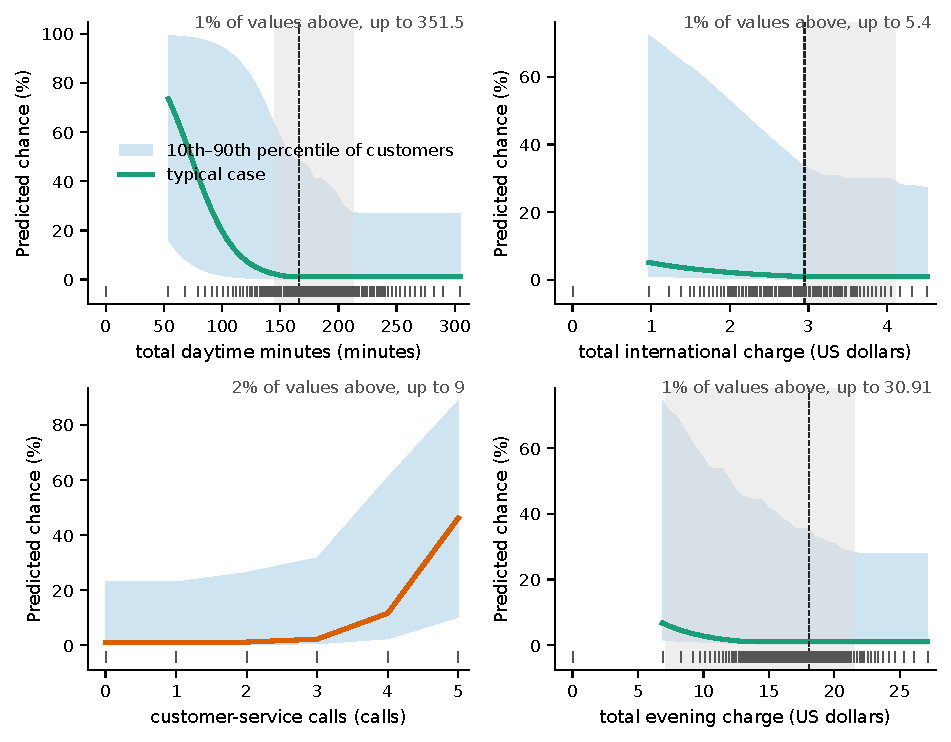
\includegraphics[width=\linewidth,height=0.88\textheight,keepaspectratio]{figures/churn100-s2-c2/ann_96-response.pdf}
\caption{Service calls: Response curves through this part: the typical case (bold), the 10th to 90th percentile of individual customers (band), the fold or step point (dashed) with its spread across them (grey), and the observed values (ticks).}
\label{fig:churn100s2c2:plot-ann96-0}
\end{figure}
\begin{figure}[H]\centering
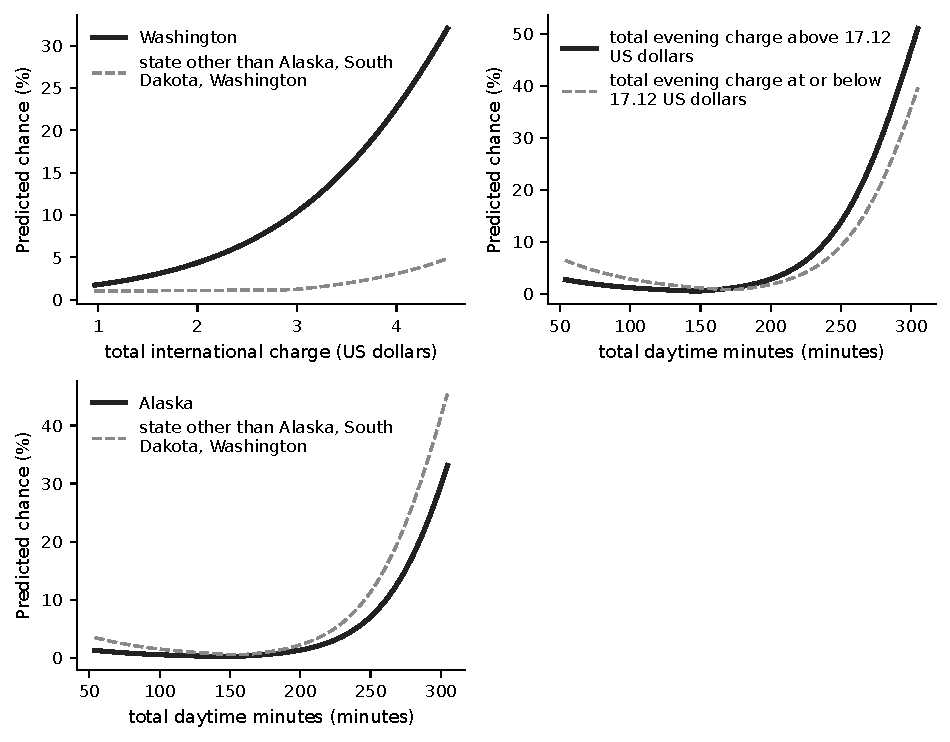
\includegraphics[width=\linewidth,height=0.88\textheight,keepaspectratio]{figures/churn100-s2-c2/ann_96-interaction.pdf}
\caption{Service calls: How the effect differs between groups: one curve per group, for the typical case of each group.}
\label{fig:churn100s2c2:plot-ann96-1}
\end{figure}
\begin{figure}[H]\centering
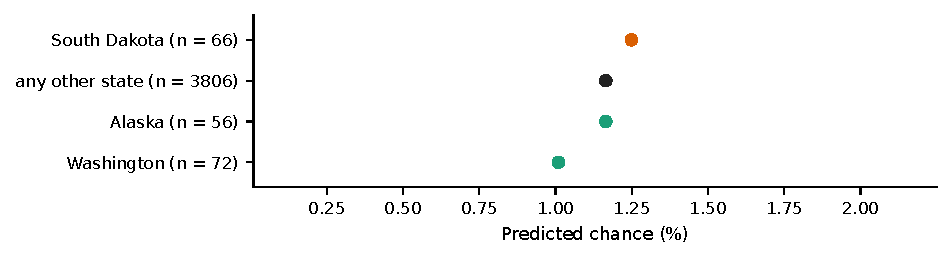
\includegraphics[width=\linewidth,height=0.88\textheight,keepaspectratio]{figures/churn100-s2-c2/ann_96-categories-small.pdf}
\caption{Service calls: The predicted value for the typical case at each level, through this part (n = training customers; grey: fewer than 20).}
\label{fig:churn100s2c2:plot-ann96-2}
\end{figure}
\begin{figure}[H]\centering
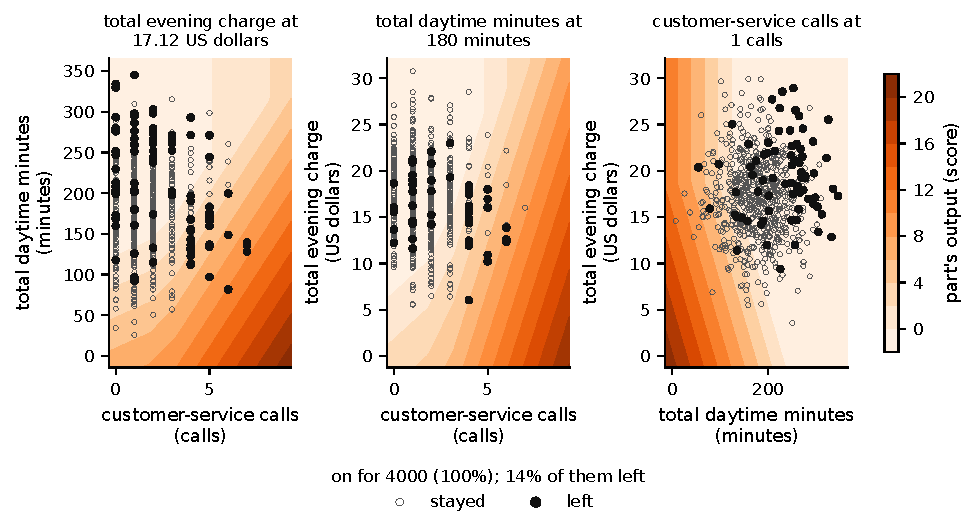
\includegraphics[width=\linewidth,height=0.88\textheight,keepaspectratio]{figures/churn100-s2-c2/ann_96-deep-map.pdf}
\caption{Service calls: The part's own output over each pair of its three main inputs (the third held at its median, named above each panel; the points are the training rows whose third input is between its 40th and 60th percentile), other inputs at the typical case: colour where it is on, flat grey where it is switched off, the black line where it switches on; training customers as hollow (no event) and filled (event) points, so the part can be seen catching the events (the predicted-chance overlay was harder to read). The switch-on line is traced on this map only; the boundary claim (C146) did not pass its check on the data, so no rule is stated.}
\label{fig:churn100s2c2:plot-ann96-3}
\end{figure}
\begin{figure}[H]\centering
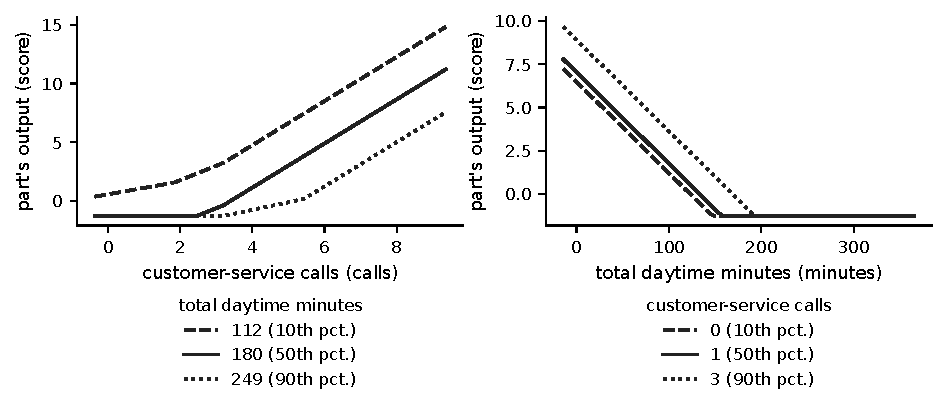
\includegraphics[width=\linewidth,height=0.88\textheight,keepaspectratio]{figures/churn100-s2-c2/ann_96-deep-slices.pdf}
\caption{Service calls: Slices of the same map: the part's own output against each input at three values of the other, so the tilted boundary shows as a shifting hinge. The switch-on line is traced on this map only; the boundary claim (C146) did not pass its check on the data, so no rule is stated.}
\label{fig:churn100s2c2:plot-ann96-4}
\end{figure}
\begin{figure}[H]\centering
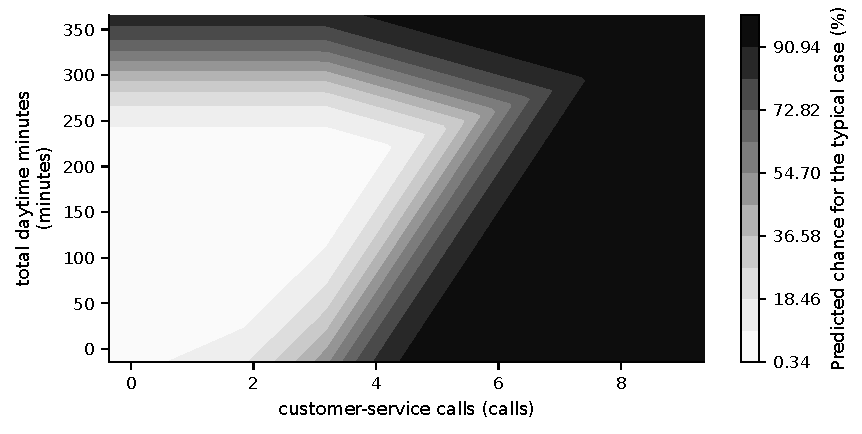
\includegraphics[width=\linewidth,height=0.88\textheight,keepaspectratio]{figures/churn100-s2-c2/ann_96-deep-risk.pdf}
\caption{Service calls: The same map on the final scale: the predicted value for the typical case, with the switch-on line (orange). The switch-on line is traced on this map only; the boundary claim (C146) did not pass its check on the data, so no rule is stated.}
\label{fig:churn100s2c2:plot-ann96-5}
\end{figure}
\begin{figure}[H]\centering
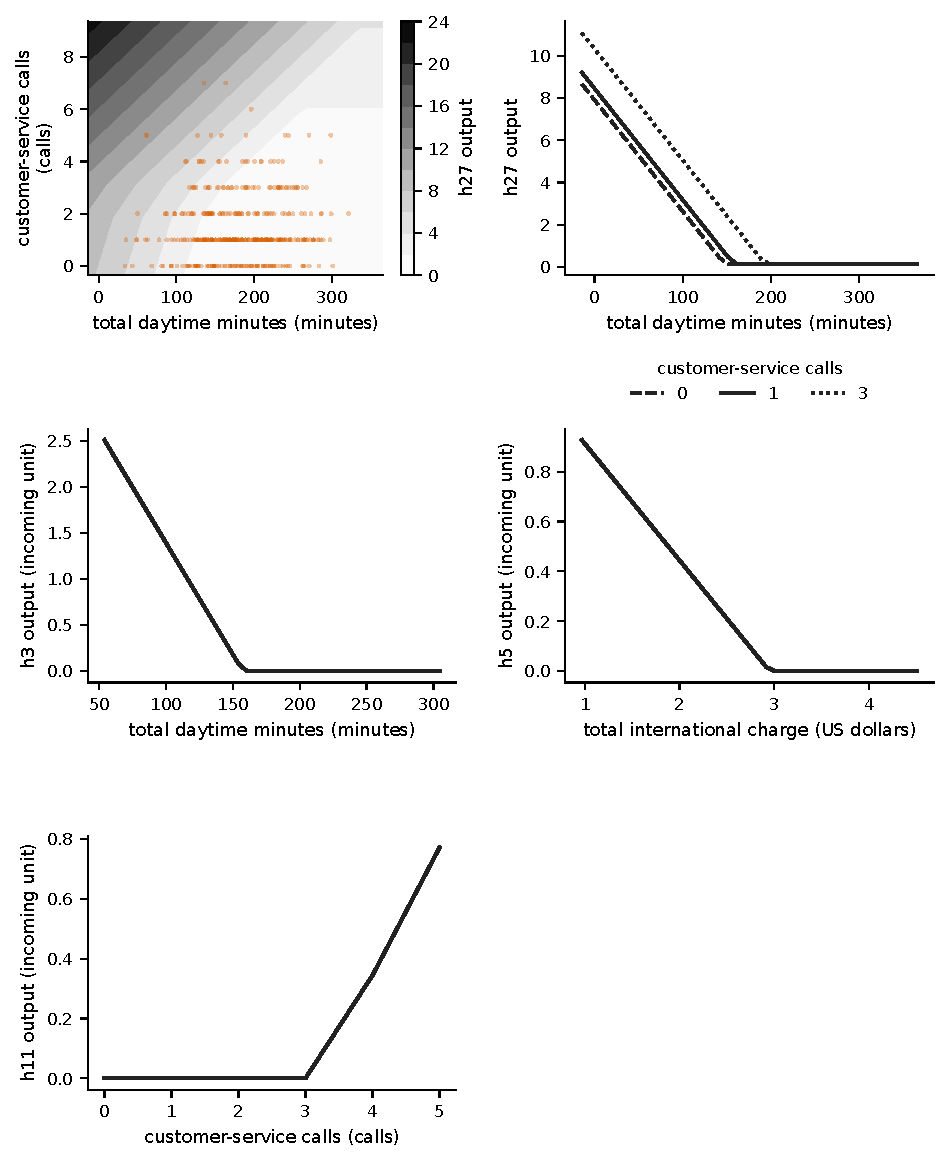
\includegraphics[width=\linewidth,height=0.88\textheight,keepaspectratio]{figures/churn100-s2-c2/ann_96-partial-identity_svc.pdf}
\caption{Service calls: This part's own output, unit h27 (combines 3 non-linear units), on its own scale (its activation), with every other input at the typical case; it is active for 3092 of 4000. Left: its output over its two main inputs (orange line: where it switches on; dots: the data); right: slices at three values of the second input; then each incoming non-linear unit against its own main input.}
\label{fig:churn100s2c2:plot-ann96-6}
\end{figure}
\begin{figure}[H]\centering
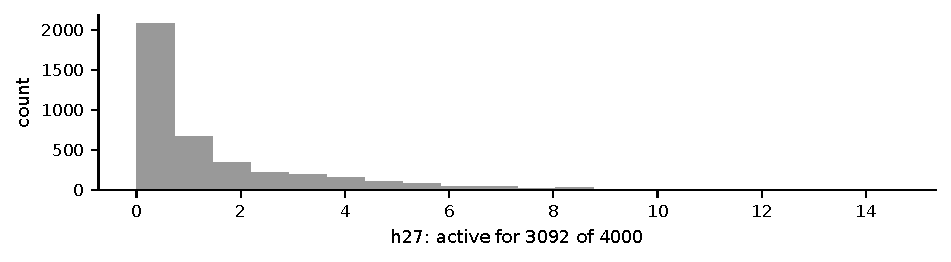
\includegraphics[width=\linewidth,height=0.88\textheight,keepaspectratio]{figures/churn100-s2-c2/ann_96-units.pdf}
\caption{Service calls: This part's hidden units: each unit's output against its main numeric input (top) and how often it is active (bottom).}
\label{fig:churn100s2c2:plot-ann96-7}
\end{figure}
\par\smallskip\noindent{\small \textbf{Dive deeper:} Calls with low usage (\ref{rd:ann90}); Many service calls (\ref{rd:ann91}). Technical detail: \ref{tech:ann96}.\par}
\subsubsection{Calls with low usage}\label{rd:ann90}
\noindent{\footnotesize Part of: Service calls (\ref{rd:ann96}).\par}
\noindent{\small Figure~\ref{fig:churn100s2c2:parts-ann90} shows what feeds this part; Figure~\ref{fig:churn100s2c2:units-ann90} its units and every connection into them (dashed boxes: connections from or to other parts, drawn in their own sections).\par}
\begin{figure}[H]\centering
\resizebox{!}{\ifdim\height>0.5\textheight 0.5\textheight\else\height\fi}{%
\resizebox{\ifdim\width>\linewidth\linewidth\else\width\fi}{!}{%
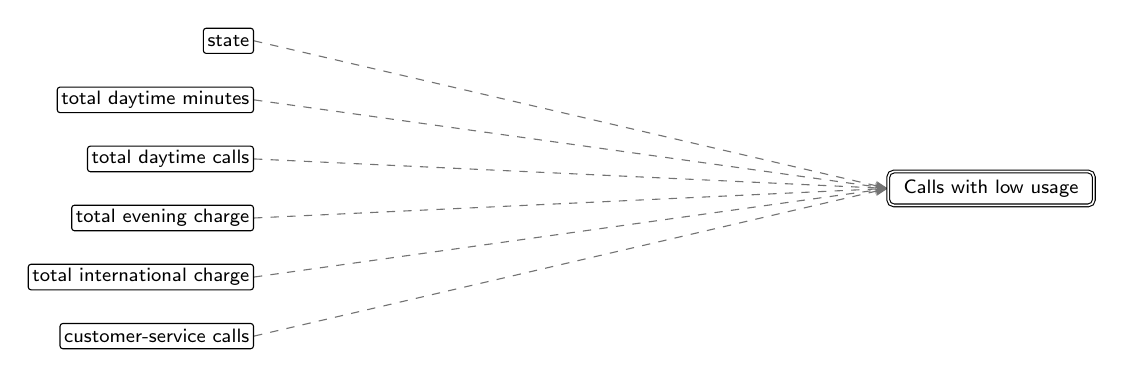
\begin{tikzpicture}[
  font=\sffamily\scriptsize, >={Stealth[length=1.6mm]},
  inp/.style={draw, rounded corners=1pt, fill=white, inner sep=1.5pt, minimum height=3.2mm, anchor=east},
  abox/.style={draw, thick, rounded corners=2pt, align=center, inner sep=3pt, minimum height=6mm, text width=42mm},
  outp/.style={draw, double, rounded corners=2pt, fill=white, align=center, inner sep=3pt, text width=24mm},
  agg/.style={draw=black!55},
]
\node[inp] (i0) at (0,1.875) {state};
\node[inp] (i1) at (0,1.125) {total daytime minutes};
\node[inp] (i2) at (0,0.375) {total daytime calls};
\node[inp] (i3) at (0,-0.375) {total evening charge};
\node[inp] (i4) at (0,-1.125) {total international charge};
\node[inp] (i5) at (0,-1.875) {customer-service calls};
\node[outp] (out) at (9.36,0) {Calls with low usage};
\begin{scope}[on background layer]
\draw[->, agg, thin, dashed] (i0.east) -- (out.west);
\draw[->, agg, thin, dashed] (i1.east) -- (out.west);
\draw[->, agg, thin, dashed] (i2.east) -- (out.west);
\draw[->, agg, thin, dashed] (i3.east) -- (out.west);
\draw[->, agg, thin, dashed] (i4.east) -- (out.west);
\draw[->, agg, thin, dashed] (i5.east) -- (out.west);
\end{scope}
\end{tikzpicture}}}%
\caption{Calls with low usage: what feeds it, one level down.}
\label{fig:churn100s2c2:parts-ann90}
\end{figure}
\begin{figure}[H]\centering
\resizebox{\ifdim\width>\linewidth\linewidth\else\width\fi}{!}{%
\definecolor{netup}{HTML}{D95F02}\definecolor{netdown}{HTML}{1B9E77}\definecolor{netmixed}{HTML}{7F7F7F}%
\begin{tikzpicture}[
  font=\sffamily\scriptsize, >={Stealth[length=1.4mm]},
  inp/.style={draw, circle, fill=white, minimum size=3.2mm, inner sep=0pt},
  hid/.style={draw, circle, fill=white, minimum size=5.2mm, inner sep=0.5pt, font=\sffamily\tiny},
  exitbox/.style={draw, thick, rectangle, fill=white, align=center, text width=17mm, minimum height=5mm, inner sep=1.5pt, font=\sffamily\tiny},
  sumbox/.style={draw, thick, dashed, rectangle, fill=white, align=center, text width=17mm, minimum height=5mm, inner sep=1.5pt, font=\sffamily\tiny},
  outp/.style={draw, thick, regular polygon, regular polygon sides=6, fill=white, minimum size=10mm, inner sep=0pt, font=\sffamily\tiny, align=center},
  stub/.style={draw, dashed, rounded corners=2pt, fill=white, align=center, inner sep=2pt, font=\sffamily\tiny, text width=15mm},
  inlab/.style={font=\sffamily\tiny, align=center, text width=15mm, inner sep=1pt, fill=white, fill opacity=0.8, text opacity=1},
  wpos/.style={draw=NavyBlue}, wneg/.style={draw=BrickRed}, wagg/.style={draw=black!45, line width=1.2pt},
  wmix/.style={draw=Plum},
]
\node[hid] (n15509) at (4.65,1.9) {h23};
\node[hid] (n2627) at (4.65,3.25) {h6};
\node[hid] (n2796) at (6.15,3.25) {h7};
\node[hid] (n9555) at (6.15,1.9) {h15};
\node[hid] (n1264) at (5.4,5.95) {h5};
\node[hid] (n807) at (5.4,4.6) {h3};
\node[inp, draw=netup, very thick] (ninxxtotalxdayxcalls) at (2.7,0.0) {};
\path (ninxxtotalxdayxcalls.south) node[inlab, anchor=north] (labninxxtotalxdayxcalls) {total daytime calls $\uparrow$};
\node[inp, draw=netdown, very thick] (ninxxtotalxintlxcharge) at (6.3,0.0) {};
\path (ninxxtotalxintlxcharge.south) node[inlab, anchor=north] (labninxxtotalxintlxcharge) {total international charge $\downarrow$};
\node[inp, draw=netdown, very thick] (ninxxtotalxevexcharge) at (9.9,0.0) {};
\path (ninxxtotalxevexcharge.south) node[inlab, anchor=north] (labninxxtotalxevexcharge) {total evening charge $\downarrow$};
\node[inp, draw=netdown, very thick] (ninxxtotalxdayxminutes) at (4.5,0.0) {};
\path (ninxxtotalxdayxminutes.south) node[inlab, anchor=north] (labninxxtotalxdayxminutes) {total daytime minutes $\downarrow$};
\node[inp, draw=netmixed, very thick] (ngrpxxstate) at (8.1,0.0) {};
\path (ngrpxxstate.south) node[inlab, anchor=north] (labngrpxxstate) {state (26 of 51 used) $\updownarrow$};
\node[inp, draw=netup, very thick] (ninxxnumberxcustomerxservicexcalls) at (0.9,0.0) {};
\path (ninxxnumberxcustomerxservicexcalls.south) node[inlab, anchor=north] (labninxxnumberxcustomerxservicexcalls) {customer-service calls $\uparrow$};
\node[stub] (ntoxxServicexcalls) at (5.4,7.5) {to Service calls};
\begin{scope}[on background layer]
\node[fit=(n15509) (n2627) (n2796) (n9555) (n1264) (n807) , inner sep=8pt, rounded corners=5pt, fill=ForestGreen!10, draw=ForestGreen!45] (clu0) {};
\draw[->, wpos, line width=0.27pt] (ninxxtotalxdayxcalls) -- (n807);
\draw[->, wpos, line width=0.46pt] (n2627) -- (n807);
\draw[->, wpos, line width=0.45pt] (n2796) -- (n807);
\draw[->, wpos, line width=0.37pt] (n807) -- (n1264);
\draw[->, wpos, line width=0.38pt] (n9555) -- (n2627);
\draw[->, wpos, line width=0.38pt] (n15509) -- (n2796);
\draw[->, wneg, line width=0.37pt] (ninxxtotalxintlxcharge) -- (n1264);
\draw[->, wneg, line width=0.60pt] (ninxxtotalxevexcharge) -- (n2796);
\draw[->, wneg, line width=0.71pt] (ninxxtotalxdayxminutes) -- (n807);
\draw[->, wpos, line width=0.33pt] (ninxxnumberxcustomerxservicexcalls) -- (n2627);
\draw[->, wpos, line width=0.36pt] (ninxxnumberxcustomerxservicexcalls) -- (n2796);
\draw[->, wpos, line width=0.57pt] (ninxxnumberxcustomerxservicexcalls) -- (n9555);
\draw[->, wpos, line width=0.60pt] (ninxxnumberxcustomerxservicexcalls) -- (n15509);
\draw[->, wpos, line width=0.80pt] (n807) -- (ntoxxServicexcalls);
\draw[->, wpos, line width=0.88pt] (n1264) -- (ntoxxServicexcalls);
\draw[->, wneg, line width=0.39pt] (ngrpxxstate) -- node[pos=0.8, sloped, above, font=\sffamily\tiny, inner sep=1pt, fill=white, fill opacity=0.8, text opacity=1] {-0.40} (n1264);
\draw[->, wmix, line width=0.74pt] (ngrpxxstate) -- node[pos=0.8, sloped, above, font=\sffamily\tiny, inner sep=1pt, fill=white, fill opacity=0.8, text opacity=1] {2 edges, -1.41 to +0.13} (n2796);
\end{scope}
\node[font=\sffamily\scriptsize\bfseries, text=ForestGreen!55!black, anchor=south west, inner sep=1pt, fill=white, fill opacity=0.85, text opacity=1] at (clu0.north west) {Calls with low usage};
\end{tikzpicture}}%
\caption{Calls with low usage: its units and every connection into them. Blue: positive weight (raises the score); red: negative weight (lowers it); thicker: larger weight. Orange outline and up arrow: raises the final prediction; teal and down arrow: lowers it; grey and double arrow: depends.}
\label{fig:churn100s2c2:units-ann90}
\end{figure}
\paragraph{Hypothesis.} This part raises the chance of leaving for customers with low usage, more so when they call customer service: daytime minutes lower it only while they stay below about 166 minutes (between 145 and 213 minutes for different customers), and calls raise it, both in an uneven way.\,{\scriptsize\textcolor{NavyBlue}{[C112, C106]}}
\paragraph{Evidence.} It acts on 3063 of 4000 training customers, 393 of whom left; for the typical customer it acts on, it changes the chance by less than a point.\,{\scriptsize\textcolor{NavyBlue}{[C117]}} Through it, a typical customer's chance falls in an uneven way from about 28\% at 91 minutes of daytime use to about 1\% at 352 minutes, with no further fall past about 166 minutes (between 145 and 213 minutes for different customers).\,{\scriptsize\textcolor{NavyBlue}{[C112]}} A higher international charge lowers it steadily up to about 2.95 US dollars (between 2.95 and 4.10 US dollars for different customers), then no further: for a typical such customer, from about 4\% to about 1\%.\,{\scriptsize\textcolor{NavyBlue}{[C115]}} Customer-service calls raise it in an uneven way, from about 1\% at 0 calls to about 2\% at 3 calls.\,{\scriptsize\textcolor{NavyBlue}{[C106]}} Its formula reproduces the part exactly on all 4000 training customers.\,{\scriptsize\textcolor{NavyBlue}{[C118]}}
\par\noindent{\small Evidence plots: Figure~\ref{fig:churn100s2c2:plot-ann90-0}, Figure~\ref{fig:churn100s2c2:plot-ann90-1}, Figure~\ref{fig:churn100s2c2:plot-ann90-2}, Figure~\ref{fig:churn100s2c2:plot-ann90-3}, Figure~\ref{fig:churn100s2c2:plot-ann90-4}, Figure~\ref{fig:churn100s2c2:plot-ann90-5}, Figure~\ref{fig:churn100s2c2:plot-ann90-6}, Figure~\ref{fig:churn100s2c2:plot-ann90-7}.\par}
\par\noindent{\small Figure~\ref{fig:churn100s2c2:plot-ann90-5} shows this part's own output, unit h3: over its two main inputs, with the line where it switches on.\par}
\par\noindent{\small Figure~\ref{fig:churn100s2c2:plot-ann90-6} shows this part's own output, unit h5: over its two main inputs, with the line where it switches on.\par}
\begin{figure}[H]\centering
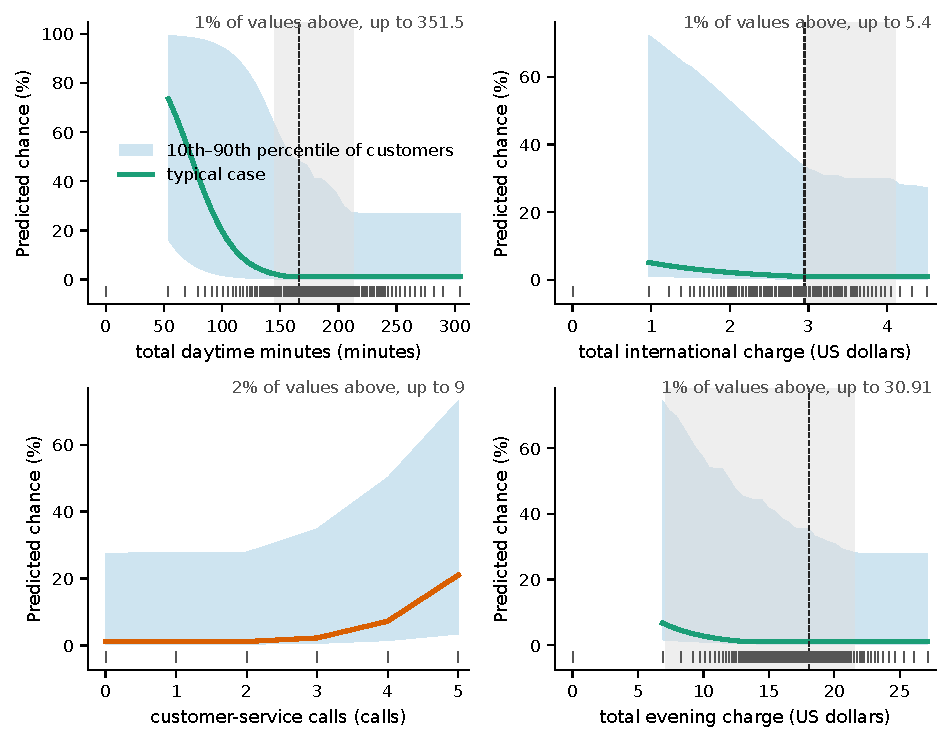
\includegraphics[width=\linewidth,height=0.88\textheight,keepaspectratio]{figures/churn100-s2-c2/ann_90-response.pdf}
\caption{Calls with low usage: Response curves through this part: the typical case (bold), the 10th to 90th percentile of individual customers (band), the fold or step point (dashed) with its spread across them (grey), and the observed values (ticks).}
\label{fig:churn100s2c2:plot-ann90-0}
\end{figure}
\begin{figure}[H]\centering
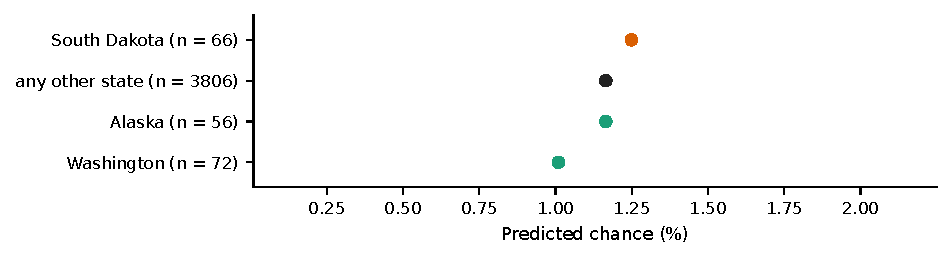
\includegraphics[width=\linewidth,height=0.88\textheight,keepaspectratio]{figures/churn100-s2-c2/ann_90-categories-small.pdf}
\caption{Calls with low usage: The predicted value for the typical case at each level, through this part (n = training customers; grey: fewer than 20).}
\label{fig:churn100s2c2:plot-ann90-1}
\end{figure}
\begin{figure}[H]\centering
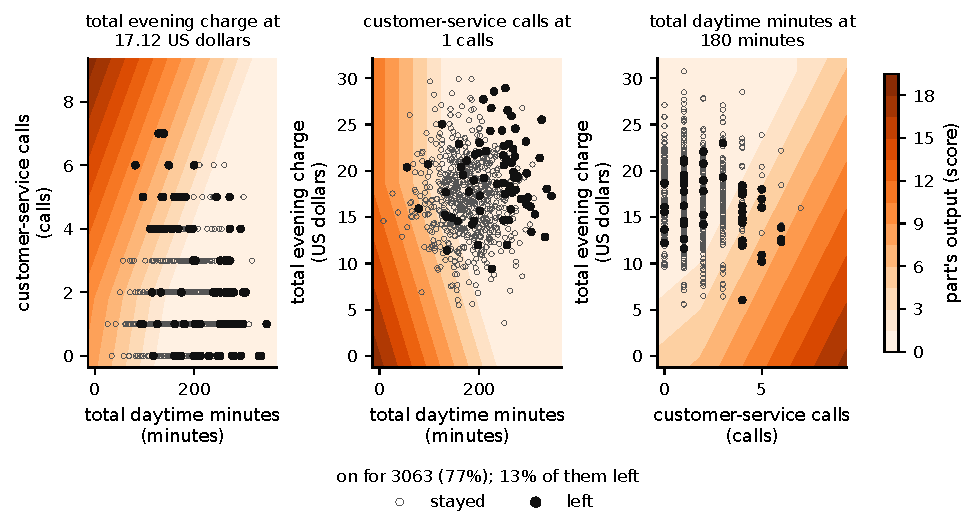
\includegraphics[width=\linewidth,height=0.88\textheight,keepaspectratio]{figures/churn100-s2-c2/ann_90-deep-map.pdf}
\caption{Calls with low usage: The part's own output over each pair of its three main inputs (the third held at its median, named above each panel; the points are the training rows whose third input is between its 40th and 60th percentile), other inputs at the typical case: colour where it is on, flat grey where it is switched off, the black line where it switches on; training customers as hollow (no event) and filled (event) points, so the part can be seen catching the events (the predicted-chance overlay was harder to read). The switch-on line is traced on this map only; the boundary claim (C147) did not pass its check on the data, so no rule is stated.}
\label{fig:churn100s2c2:plot-ann90-2}
\end{figure}
\begin{figure}[H]\centering
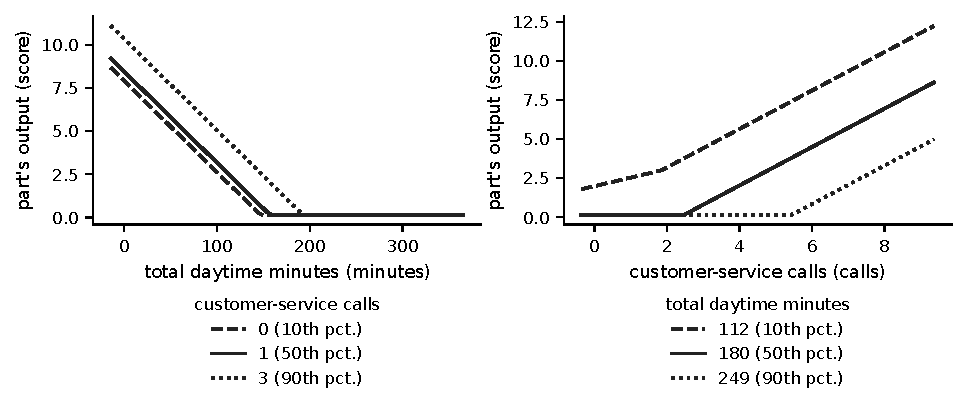
\includegraphics[width=\linewidth,height=0.88\textheight,keepaspectratio]{figures/churn100-s2-c2/ann_90-deep-slices.pdf}
\caption{Calls with low usage: Slices of the same map: the part's own output against each input at three values of the other, so the tilted boundary shows as a shifting hinge. The switch-on line is traced on this map only; the boundary claim (C147) did not pass its check on the data, so no rule is stated.}
\label{fig:churn100s2c2:plot-ann90-3}
\end{figure}
\begin{figure}[H]\centering
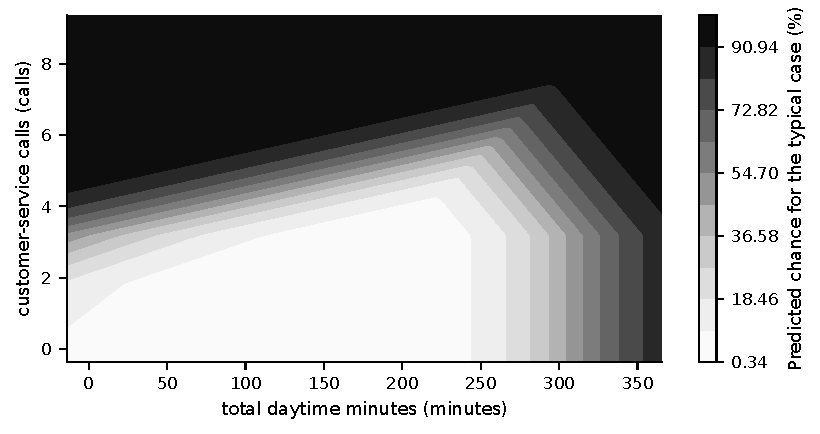
\includegraphics[width=\linewidth,height=0.88\textheight,keepaspectratio]{figures/churn100-s2-c2/ann_90-deep-risk.pdf}
\caption{Calls with low usage: The same map on the final scale: the predicted value for the typical case, with the switch-on line (orange). The switch-on line is traced on this map only; the boundary claim (C147) did not pass its check on the data, so no rule is stated.}
\label{fig:churn100s2c2:plot-ann90-4}
\end{figure}
\begin{figure}[H]\centering
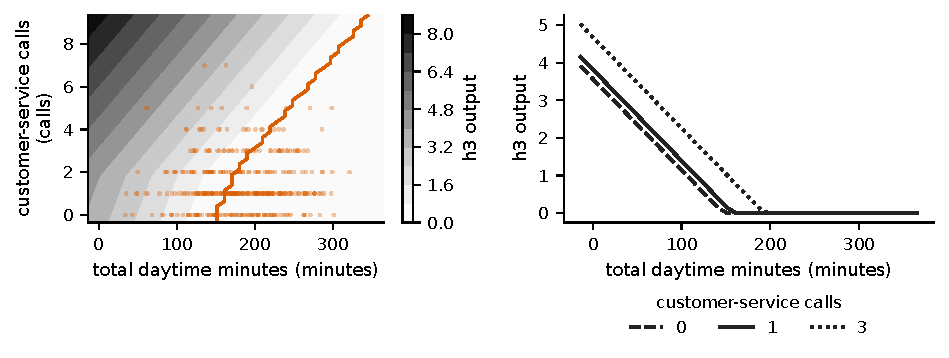
\includegraphics[width=\linewidth,height=0.88\textheight,keepaspectratio]{figures/churn100-s2-c2/ann_90-partial-807.pdf}
\caption{Calls with low usage: This part's own output, unit h3 (the output of 'Calls with low usage'), on its own scale (its activation), with every other input at the typical case; it is active for 1744 of 4000. Left: its output over its two main inputs (orange line: where it switches on; dots: the data); right: slices at three values of the second input.}
\label{fig:churn100s2c2:plot-ann90-5}
\end{figure}
\begin{figure}[H]\centering
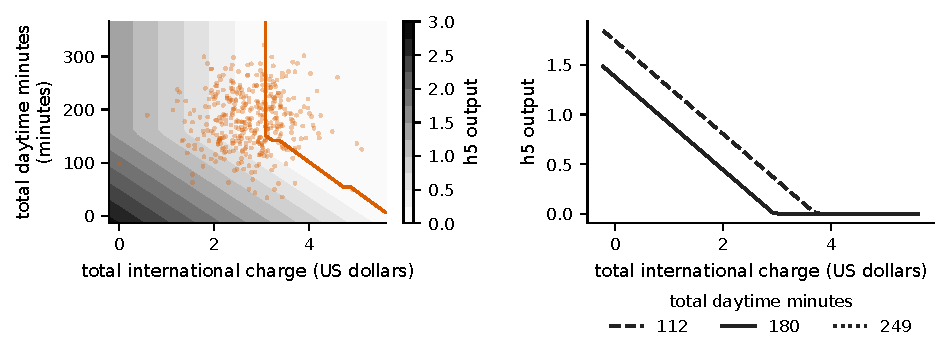
\includegraphics[width=\linewidth,height=0.88\textheight,keepaspectratio]{figures/churn100-s2-c2/ann_90-partial-1264.pdf}
\caption{Calls with low usage: This part's own output, unit h5 (the output of 'Calls with low usage'), on its own scale (its activation), with every other input at the typical case; it is active for 2771 of 4000. Left: its output over its two main inputs (orange line: where it switches on; dots: the data); right: slices at three values of the second input.}
\label{fig:churn100s2c2:plot-ann90-6}
\end{figure}
\begin{figure}[H]\centering
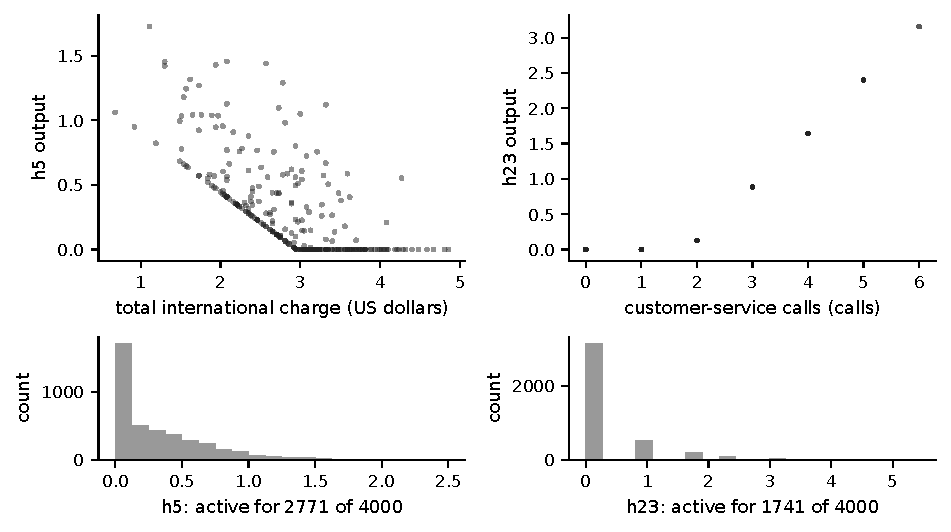
\includegraphics[width=\linewidth,height=0.88\textheight,keepaspectratio]{figures/churn100-s2-c2/ann_90-units.pdf}
\caption{Calls with low usage: This part's hidden units: each unit's output against its main numeric input (top) and how often it is active (bottom).}
\label{fig:churn100s2c2:plot-ann90-7}
\end{figure}
\par\smallskip\noindent{\small Technical detail: \ref{tech:ann90}.\par}
\subsubsection{Many service calls}\label{rd:ann91}
\noindent{\footnotesize Part of: Service calls (\ref{rd:ann96}).\par}
\noindent{\small Figure~\ref{fig:churn100s2c2:parts-ann91} shows what feeds this part; Figure~\ref{fig:churn100s2c2:units-ann91} its units and every connection into them (dashed boxes: connections from or to other parts, drawn in their own sections).\par}
\begin{figure}[H]\centering
\resizebox{!}{\ifdim\height>0.5\textheight 0.5\textheight\else\height\fi}{%
\resizebox{\ifdim\width>\linewidth\linewidth\else\width\fi}{!}{%
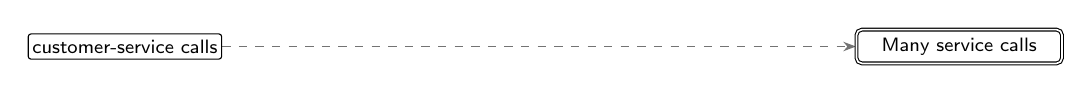
\begin{tikzpicture}[
  font=\sffamily\scriptsize, >={Stealth[length=1.6mm]},
  inp/.style={draw, rounded corners=1pt, fill=white, inner sep=1.5pt, minimum height=3.2mm, anchor=east},
  abox/.style={draw, thick, rounded corners=2pt, align=center, inner sep=3pt, minimum height=6mm, text width=42mm},
  outp/.style={draw, double, rounded corners=2pt, fill=white, align=center, inner sep=3pt, text width=24mm},
  agg/.style={draw=black!55},
]
\node[inp] (i0) at (0,-0.0) {customer-service calls};
\node[outp] (out) at (9.36,0) {Many service calls};
\begin{scope}[on background layer]
\draw[->, agg, thin, dashed] (i0.east) -- (out.west);
\end{scope}
\end{tikzpicture}}}%
\caption{Many service calls: what feeds it, one level down.}
\label{fig:churn100s2c2:parts-ann91}
\end{figure}
\begin{figure}[H]\centering
\resizebox{\ifdim\width>\linewidth\linewidth\else\width\fi}{!}{%
\definecolor{netup}{HTML}{D95F02}\definecolor{netdown}{HTML}{1B9E77}\definecolor{netmixed}{HTML}{7F7F7F}%
\begin{tikzpicture}[
  font=\sffamily\scriptsize, >={Stealth[length=1.4mm]},
  inp/.style={draw, circle, fill=white, minimum size=3.2mm, inner sep=0pt},
  hid/.style={draw, circle, fill=white, minimum size=5.2mm, inner sep=0.5pt, font=\sffamily\tiny},
  exitbox/.style={draw, thick, rectangle, fill=white, align=center, text width=17mm, minimum height=5mm, inner sep=1.5pt, font=\sffamily\tiny},
  sumbox/.style={draw, thick, dashed, rectangle, fill=white, align=center, text width=17mm, minimum height=5mm, inner sep=1.5pt, font=\sffamily\tiny},
  outp/.style={draw, thick, regular polygon, regular polygon sides=6, fill=white, minimum size=10mm, inner sep=0pt, font=\sffamily\tiny, align=center},
  stub/.style={draw, dashed, rounded corners=2pt, fill=white, align=center, inner sep=2pt, font=\sffamily\tiny, text width=15mm},
  inlab/.style={font=\sffamily\tiny, align=center, text width=15mm, inner sep=1pt, fill=white, fill opacity=0.8, text opacity=1},
  wpos/.style={draw=NavyBlue}, wneg/.style={draw=BrickRed}, wagg/.style={draw=black!45, line width=1.2pt},
  wmix/.style={draw=Plum},
]
\node[exitbox] (n7208) at (1.8,1.9) {Many service calls $\uparrow$};
\node[inp, draw=netup, very thick] (ninxxnumberxcustomerxservicexcalls) at (1.8,0.0) {};
\path (ninxxnumberxcustomerxservicexcalls.south) node[inlab, anchor=north] (labninxxnumberxcustomerxservicexcalls) {customer-service calls $\uparrow$};
\node[stub] (ntoxxServicexcalls) at (1.8,3.45) {to Service calls};
\begin{scope}[on background layer]
\node[fit=(n7208) , inner sep=8pt, rounded corners=5pt, fill=ForestGreen!10, draw=ForestGreen!45] (clu0) {};
\draw[->, wpos, line width=0.45pt] (ninxxnumberxcustomerxservicexcalls) -- (n7208);
\draw[->, wpos, line width=0.78pt] (n7208) -- (ntoxxServicexcalls);
\end{scope}
\node[font=\sffamily\scriptsize\bfseries, text=ForestGreen!55!black, anchor=south west, inner sep=1pt, fill=white, fill opacity=0.85, text opacity=1] at (clu0.north west) {Many service calls};
\end{tikzpicture}}%
\caption{Many service calls: its units and every connection into them. Blue: positive weight (raises the score); red: negative weight (lowers it); thicker: larger weight. Orange outline and up arrow: raises the final prediction; teal and down arrow: lowers it; grey and double arrow: depends.}
\label{fig:churn100s2c2:units-ann91}
\end{figure}
\paragraph{Hypothesis.} This part raises the chance of leaving from 4 customer-service calls upwards, slowly at first, then faster.\,{\scriptsize\textcolor{NavyBlue}{[C122]}}
\paragraph{Evidence.} It acts on 318 of 4000 training customers, 159 of whom left; for the typical customer it acts on, the chance is about 7\% without it and about 12\% with it.\,{\scriptsize\textcolor{NavyBlue}{[C123]}} Through it, the chance rises slowly at first, then faster: going from 0 to 4 calls moves a typical such customer's chance from about 1\% to about 2\%.\,{\scriptsize\textcolor{NavyBlue}{[C122]}} Its formula reproduces the part exactly on all 4000 training customers.\,{\scriptsize\textcolor{NavyBlue}{[C124]}}
\par\noindent{\small Evidence plots: Figure~\ref{fig:churn100s2c2:plot-ann91-0}, Figure~\ref{fig:churn100s2c2:plot-ann91-1}.\par}
\par\noindent{\small Figure~\ref{fig:churn100s2c2:plot-ann91-0} shows this part's own output, unit h11: it switches on at about 3.194 calls of customer-service calls, and is zero below.\par}
\begin{figure}[H]\centering
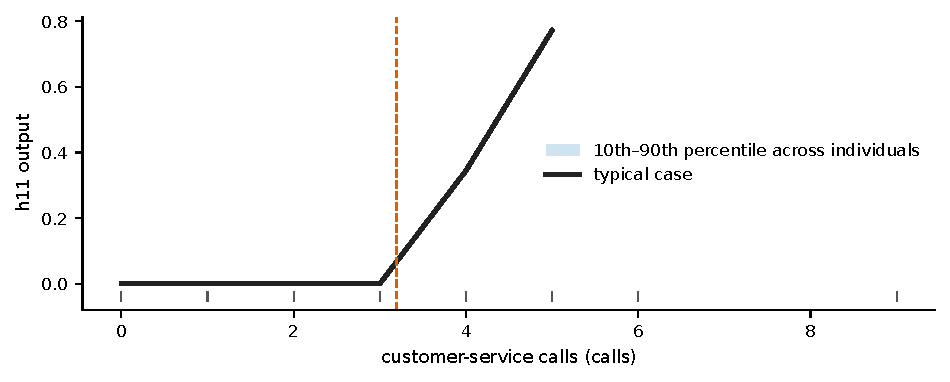
\includegraphics[width=\linewidth,height=0.88\textheight,keepaspectratio]{figures/churn100-s2-c2/ann_91-partial-7208.pdf}
\caption{Many service calls: This part's own output, unit h11 (the output of 'Many service calls'), on its own scale (its activation), with every other input at the typical case; it is active for 318 of 4000. Bold: the typical case; band: 10th to 90th percentile across individuals; dashed: where it switches on; ticks: the data.}
\label{fig:churn100s2c2:plot-ann91-0}
\end{figure}
\begin{figure}[H]\centering
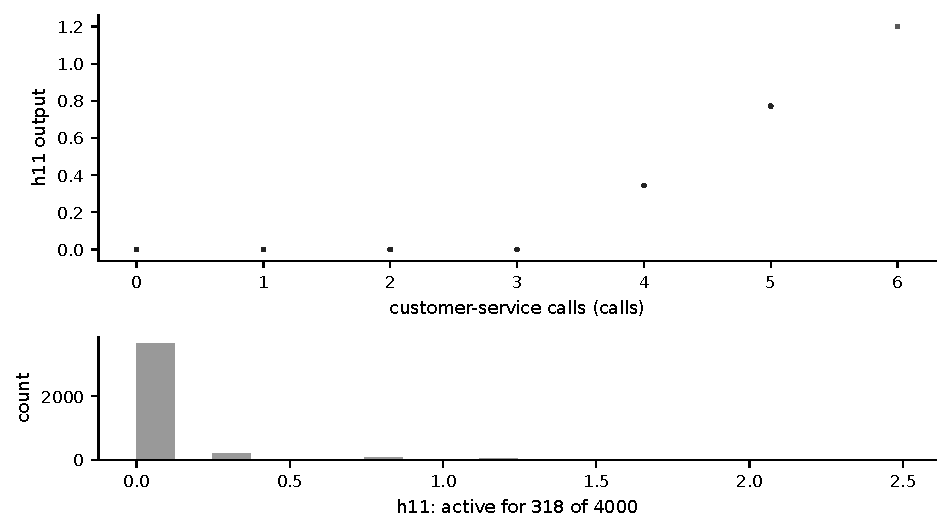
\includegraphics[width=\linewidth,height=0.88\textheight,keepaspectratio]{figures/churn100-s2-c2/ann_91-units.pdf}
\caption{Many service calls: This part's hidden units: each unit's output against its main numeric input (top) and how often it is active (bottom).}
\label{fig:churn100s2c2:plot-ann91-1}
\end{figure}
\par\smallskip\noindent{\small Technical detail: \ref{tech:ann91}.\par}
\subsubsection{Voice-mail discount}\label{rd:ann92}
\noindent{\footnotesize Part of: The whole model (\ref{rd:ann97}).\par}
\noindent{\small Figure~\ref{fig:churn100s2c2:parts-ann92} shows what feeds this part; Figure~\ref{fig:churn100s2c2:units-ann92} its units and every connection into them (dashed boxes: connections from or to other parts, drawn in their own sections).\par}
\begin{figure}[H]\centering
\resizebox{!}{\ifdim\height>0.5\textheight 0.5\textheight\else\height\fi}{%
\resizebox{\ifdim\width>\linewidth\linewidth\else\width\fi}{!}{%
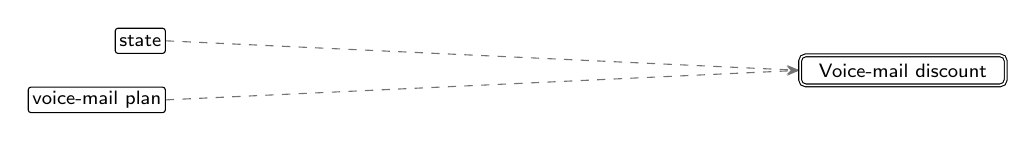
\begin{tikzpicture}[
  font=\sffamily\scriptsize, >={Stealth[length=1.6mm]},
  inp/.style={draw, rounded corners=1pt, fill=white, inner sep=1.5pt, minimum height=3.2mm, anchor=east},
  abox/.style={draw, thick, rounded corners=2pt, align=center, inner sep=3pt, minimum height=6mm, text width=42mm},
  outp/.style={draw, double, rounded corners=2pt, fill=white, align=center, inner sep=3pt, text width=24mm},
  agg/.style={draw=black!55},
]
\node[inp] (i0) at (0,0.375) {state};
\node[inp] (i1) at (0,-0.375) {voice-mail plan};
\node[outp] (out) at (9.36,0) {Voice-mail discount};
\begin{scope}[on background layer]
\draw[->, agg, thin, dashed] (i0.east) -- (out.west);
\draw[->, agg, thin, dashed] (i1.east) -- (out.west);
\end{scope}
\end{tikzpicture}}}%
\caption{Voice-mail discount: what feeds it, one level down.}
\label{fig:churn100s2c2:parts-ann92}
\end{figure}
\begin{figure}[H]\centering
\resizebox{\ifdim\width>\linewidth\linewidth\else\width\fi}{!}{%
\definecolor{netup}{HTML}{D95F02}\definecolor{netdown}{HTML}{1B9E77}\definecolor{netmixed}{HTML}{7F7F7F}%
\begin{tikzpicture}[
  font=\sffamily\scriptsize, >={Stealth[length=1.4mm]},
  inp/.style={draw, circle, fill=white, minimum size=3.2mm, inner sep=0pt},
  hid/.style={draw, circle, fill=white, minimum size=5.2mm, inner sep=0.5pt, font=\sffamily\tiny},
  exitbox/.style={draw, thick, rectangle, fill=white, align=center, text width=17mm, minimum height=5mm, inner sep=1.5pt, font=\sffamily\tiny},
  sumbox/.style={draw, thick, dashed, rectangle, fill=white, align=center, text width=17mm, minimum height=5mm, inner sep=1.5pt, font=\sffamily\tiny},
  outp/.style={draw, thick, regular polygon, regular polygon sides=6, fill=white, minimum size=10mm, inner sep=0pt, font=\sffamily\tiny, align=center},
  stub/.style={draw, dashed, rounded corners=2pt, fill=white, align=center, inner sep=2pt, font=\sffamily\tiny, text width=15mm},
  inlab/.style={font=\sffamily\tiny, align=center, text width=15mm, inner sep=1pt, fill=white, fill opacity=0.8, text opacity=1},
  wpos/.style={draw=NavyBlue}, wneg/.style={draw=BrickRed}, wagg/.style={draw=black!45, line width=1.2pt},
  wmix/.style={draw=Plum},
]
\node[hid] (n4051) at (1.9,4.6) {h8};
\node[hid] (n1133) at (1.9,3.25) {h4};
\node[hid] (n14955) at (1.9,1.9) {h22};
\node[hid] (n13852) at (0.4,1.9) {h20};
\node[hid] (n5577) at (3.4,1.9) {h10};
\node[inp, draw=netmixed, very thick] (ngrpxxstate) at (1.0,0.0) {};
\path (ngrpxxstate.south) node[inlab, anchor=north] (labngrpxxstate) {state (26 of 51 used) $\updownarrow$};
\node[inp, draw=netdown, very thick] (ninxxvoicexmailxplan) at (2.8,0.0) {};
\path (ninxxvoicexmailxplan.south) node[inlab, anchor=north] (labninxxvoicexmailxplan) {a voice-mail plan $\downarrow$};
\node[stub] (ntoxxthexmodelxoutput) at (1.9,6.15) {to the model output};
\begin{scope}[on background layer]
\node[fit=(n4051) (n1133) (n14955) (n13852) (n5577) , inner sep=8pt, rounded corners=5pt, fill=Orchid!10, draw=Orchid!45] (clu0) {};
\draw[->, wpos, line width=0.58pt] (n1133) -- (n4051);
\draw[->, wpos, line width=0.32pt] (n5577) -- (n1133);
\draw[->, wpos, line width=0.33pt] (n13852) -- (n1133);
\draw[->, wpos, line width=0.26pt] (n14955) -- (n1133);
\draw[->, wpos, line width=0.29pt] (ninxxvoicexmailxplan) -- (n1133);
\draw[->, wpos, line width=0.59pt] (ninxxvoicexmailxplan) -- (n5577);
\draw[->, wpos, line width=0.60pt] (ninxxvoicexmailxplan) -- (n13852);
\draw[->, wneg, line width=0.56pt] (n1133) -- (ntoxxthexmodelxoutput);
\draw[->, wneg, line width=0.60pt] (n4051) -- (ntoxxthexmodelxoutput);
\draw[->, wpos, line width=0.60pt] (ngrpxxstate) -- node[pos=0.8, sloped, above, font=\sffamily\tiny, inner sep=1pt, fill=white, fill opacity=0.8, text opacity=1] {+0.99} (n14955);
\end{scope}
\node[font=\sffamily\scriptsize\bfseries, text=Orchid!55!black, anchor=south west, inner sep=1pt, fill=white, fill opacity=0.85, text opacity=1] at (clu0.north west) {Voice-mail discount};
\end{tikzpicture}}%
\caption{Voice-mail discount: its units and every connection into them. Blue: positive weight (raises the score); red: negative weight (lowers it); thicker: larger weight. Orange outline and up arrow: raises the final prediction; teal and down arrow: lowers it; grey and double arrow: depends.}
\label{fig:churn100s2c2:units-ann92}
\end{figure}
\paragraph{Hypothesis.} This part gives customers with a voice-mail plan a further discount on the chance of leaving.\,{\scriptsize\textcolor{NavyBlue}{[C119]}}
\paragraph{Evidence.} Through it, a voice-mail plan lowers a typical customer's chance from about 1\% to under 1\%, and customers in North Carolina get under 1\% instead of about 1\%.\,{\scriptsize\textcolor{NavyBlue}{[C119, C120]}} Its formula reproduces the part exactly on all 4000 training customers.\,{\scriptsize\textcolor{NavyBlue}{[C121]}}
\par\noindent{\small Evidence plots: Figure~\ref{fig:churn100s2c2:plot-ann92-0}, Figure~\ref{fig:churn100s2c2:plot-ann92-1}.\par}
\begin{figure}[H]\centering
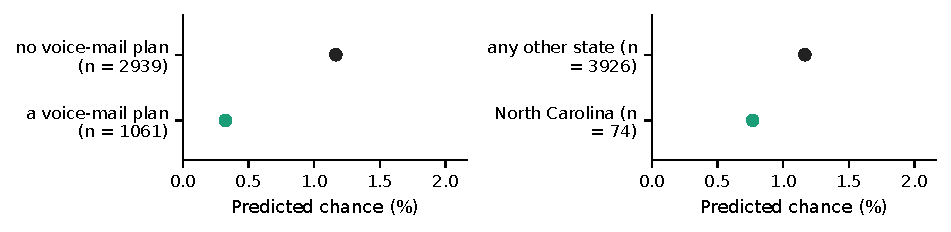
\includegraphics[width=\linewidth,height=0.88\textheight,keepaspectratio]{figures/churn100-s2-c2/ann_92-categories-small.pdf}
\caption{Voice-mail discount: The predicted value for the typical case at each level, through this part (n = training customers; grey: fewer than 20).}
\label{fig:churn100s2c2:plot-ann92-0}
\end{figure}
\begin{figure}[H]\centering
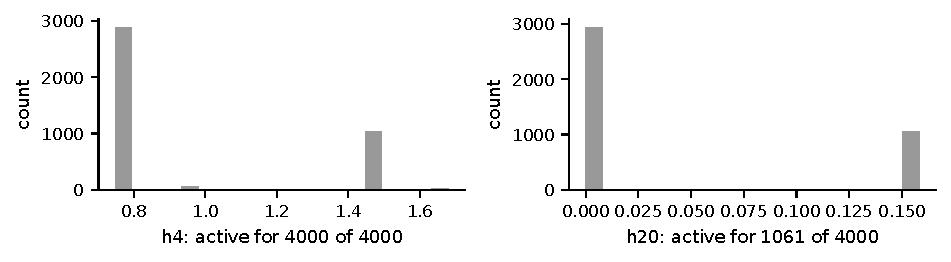
\includegraphics[width=\linewidth,height=0.88\textheight,keepaspectratio]{figures/churn100-s2-c2/ann_92-units.pdf}
\caption{Voice-mail discount: This part's hidden units: each unit's output against its main numeric input (top) and how often it is active (bottom).}
\label{fig:churn100s2c2:plot-ann92-1}
\end{figure}
\par\smallskip\noindent{\small Technical detail: \ref{tech:ann92}.\par}
\subsubsection{State units}\label{rd:ann95}
\noindent{\footnotesize Part of: The whole model (\ref{rd:ann97}).\par}
\noindent{\small Figure~\ref{fig:churn100s2c2:parts-ann95} shows what feeds this part; Figure~\ref{fig:churn100s2c2:units-ann95} its units and every connection into them (dashed boxes: connections from or to other parts, drawn in their own sections).\par}
\begin{figure}[H]\centering
\resizebox{!}{\ifdim\height>0.5\textheight 0.5\textheight\else\height\fi}{%
\resizebox{\ifdim\width>\linewidth\linewidth\else\width\fi}{!}{%
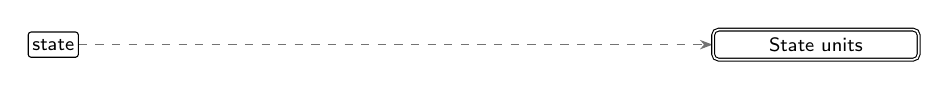
\begin{tikzpicture}[
  font=\sffamily\scriptsize, >={Stealth[length=1.6mm]},
  inp/.style={draw, rounded corners=1pt, fill=white, inner sep=1.5pt, minimum height=3.2mm, anchor=east},
  abox/.style={draw, thick, rounded corners=2pt, align=center, inner sep=3pt, minimum height=6mm, text width=42mm},
  outp/.style={draw, double, rounded corners=2pt, fill=white, align=center, inner sep=3pt, text width=24mm},
  agg/.style={draw=black!55},
]
\node[inp] (i0) at (0,-0.0) {state};
\node[outp] (out) at (9.36,0) {State units};
\begin{scope}[on background layer]
\draw[->, agg, thin, dashed] (i0.east) -- (out.west);
\end{scope}
\end{tikzpicture}}}%
\caption{State units: what feeds it, one level down.}
\label{fig:churn100s2c2:parts-ann95}
\end{figure}
\begin{figure}[H]\centering
\resizebox{\ifdim\width>\linewidth\linewidth\else\width\fi}{!}{%
\definecolor{netup}{HTML}{D95F02}\definecolor{netdown}{HTML}{1B9E77}\definecolor{netmixed}{HTML}{7F7F7F}%
\begin{tikzpicture}[
  font=\sffamily\scriptsize, >={Stealth[length=1.4mm]},
  inp/.style={draw, circle, fill=white, minimum size=3.2mm, inner sep=0pt},
  hid/.style={draw, circle, fill=white, minimum size=5.2mm, inner sep=0.5pt, font=\sffamily\tiny},
  exitbox/.style={draw, thick, rectangle, fill=white, align=center, text width=17mm, minimum height=5mm, inner sep=1.5pt, font=\sffamily\tiny},
  sumbox/.style={draw, thick, dashed, rectangle, fill=white, align=center, text width=17mm, minimum height=5mm, inner sep=1.5pt, font=\sffamily\tiny},
  outp/.style={draw, thick, regular polygon, regular polygon sides=6, fill=white, minimum size=10mm, inner sep=0pt, font=\sffamily\tiny, align=center},
  stub/.style={draw, dashed, rounded corners=2pt, fill=white, align=center, inner sep=2pt, font=\sffamily\tiny, text width=15mm},
  inlab/.style={font=\sffamily\tiny, align=center, text width=15mm, inner sep=1pt, fill=white, fill opacity=0.8, text opacity=1},
  wpos/.style={draw=NavyBlue}, wneg/.style={draw=BrickRed}, wagg/.style={draw=black!45, line width=1.2pt},
  wmix/.style={draw=Plum},
]
\node[hid] (n10332) at (0.35,1.9) {h16};
\node[hid] (n16902) at (4.85,3.25) {h25};
\node[hid] (n8418) at (9.35,1.9) {h13};
\node[hid] (n16344) at (6.35,1.9) {h24};
\node[hid] (n7647) at (6.35,3.25) {h12};
\node[hid] (n13551) at (3.35,1.9) {h18};
\node[hid] (n4967) at (7.85,1.9) {h9};
\node[hid] (n8896) at (10.85,1.9) {h14};
\node[hid] (n11261) at (1.85,1.9) {h17};
\node[hid] (n13725) at (4.85,1.9) {h19};
\node[inp, draw=netmixed, very thick] (ngrpxxstate) at (5.6,0.0) {};
\path (ngrpxxstate.south) node[inlab, anchor=north] (labngrpxxstate) {state (26 of 51 used) $\updownarrow$};
\node[stub] (ntoxxthexmodelxoutput) at (5.6,4.8) {to the model output};
\begin{scope}[on background layer]
\node[fit=(n10332) (n16902) (n8418) (n16344) (n7647) (n13551) (n4967) (n8896) (n11261) (n13725) , inner sep=8pt, rounded corners=5pt, fill=Goldenrod!10, draw=Goldenrod!45] (clu0) {};
\draw[->, wpos, line width=0.59pt] (n4967) -- (n7647);
\draw[->, wpos, line width=0.60pt] (n11261) -- (n16902);
\draw[->, wneg, line width=0.25pt] (n7647) -- (ntoxxthexmodelxoutput);
\draw[->, wneg, line width=0.25pt] (n8418) -- (ntoxxthexmodelxoutput);
\draw[->, wneg, line width=0.25pt] (n8896) -- (ntoxxthexmodelxoutput);
\draw[->, wpos, line width=0.29pt] (n10332) -- (ntoxxthexmodelxoutput);
\draw[->, wpos, line width=0.27pt] (n13551) -- (ntoxxthexmodelxoutput);
\draw[->, wpos, line width=0.27pt] (n13725) -- (ntoxxthexmodelxoutput);
\draw[->, wpos, line width=0.27pt] (n16344) -- (ntoxxthexmodelxoutput);
\draw[->, wpos, line width=0.27pt] (n16902) -- (ntoxxthexmodelxoutput);
\draw[->, wpos, line width=0.59pt] (ngrpxxstate) -- node[pos=0.8, sloped, above, font=\sffamily\tiny, inner sep=1pt, fill=white, fill opacity=0.8, text opacity=1] {+0.98} (n4967);
\draw[->, wmix, line width=0.60pt] (ngrpxxstate) -- node[pos=0.8, sloped, above, font=\sffamily\tiny, inner sep=1pt, fill=white, fill opacity=0.8, text opacity=1] {2 edges, -0.02 to +0.99} (n11261);
\draw[->, wpos, line width=0.60pt] (ngrpxxstate) -- node[pos=0.8, sloped, above, font=\sffamily\tiny, inner sep=1pt, fill=white, fill opacity=0.8, text opacity=1] {+1.00} (n13551);
\draw[->, wpos, line width=0.56pt] (ngrpxxstate) -- node[pos=0.8, sloped, above, font=\sffamily\tiny, inner sep=1pt, fill=white, fill opacity=0.8, text opacity=1] {+0.89} (n10332);
\draw[->, wpos, line width=0.60pt] (ngrpxxstate) -- node[pos=0.8, sloped, above, font=\sffamily\tiny, inner sep=1pt, fill=white, fill opacity=0.8, text opacity=1] {+1.01} (n8896);
\draw[->, wpos, line width=0.60pt] (ngrpxxstate) -- node[pos=0.8, sloped, above, font=\sffamily\tiny, inner sep=1pt, fill=white, fill opacity=0.8, text opacity=1] {+0.99} (n8418);
\draw[->, wpos, line width=0.60pt] (ngrpxxstate) -- node[pos=0.8, sloped, above, font=\sffamily\tiny, inner sep=1pt, fill=white, fill opacity=0.8, text opacity=1] {+0.99} (n13725);
\draw[->, wpos, line width=0.60pt] (ngrpxxstate) -- node[pos=0.8, sloped, above, font=\sffamily\tiny, inner sep=1pt, fill=white, fill opacity=0.8, text opacity=1] {+1.00} (n16344);
\end{scope}
\node[font=\sffamily\scriptsize\bfseries, text=Goldenrod!55!black, anchor=south west, inner sep=1pt, fill=white, fill opacity=0.85, text opacity=1] at (clu0.north west) {State units};
\end{tikzpicture}}%
\caption{State units: its units and every connection into them. Blue: positive weight (raises the score); red: negative weight (lowers it); thicker: larger weight. Orange outline and up arrow: raises the final prediction; teal and down arrow: lowers it; grey and double arrow: depends.}
\label{fig:churn100s2c2:units-ann95}
\end{figure}
\paragraph{Hypothesis.} This part reads only the state and raises the chance of leaving in a few states, most in Washington and Montana.\,{\scriptsize\textcolor{NavyBlue}{[C125, C126]}}
\paragraph{Evidence.} Through it, a typical customer's chance goes from about 1\% to about 2\% in Washington and in Montana, and up by less than a point in Kentucky and Ohio.\,{\scriptsize\textcolor{NavyBlue}{[C125, C126, C127, C128]}} In Arizona, Delaware, North Dakota and Nevada it lowers the chance by less than a tenth of a point.\,{\scriptsize\textcolor{NavyBlue}{[C129, C130, C131, C132]}} Its formula reproduces the part exactly on all 4000 training customers.\,{\scriptsize\textcolor{NavyBlue}{[C133]}}
\par\noindent{\small Evidence plots: Figure~\ref{fig:churn100s2c2:plot-ann95-0}, Figure~\ref{fig:churn100s2c2:plot-ann95-1}.\par}
\begin{figure}[H]\centering
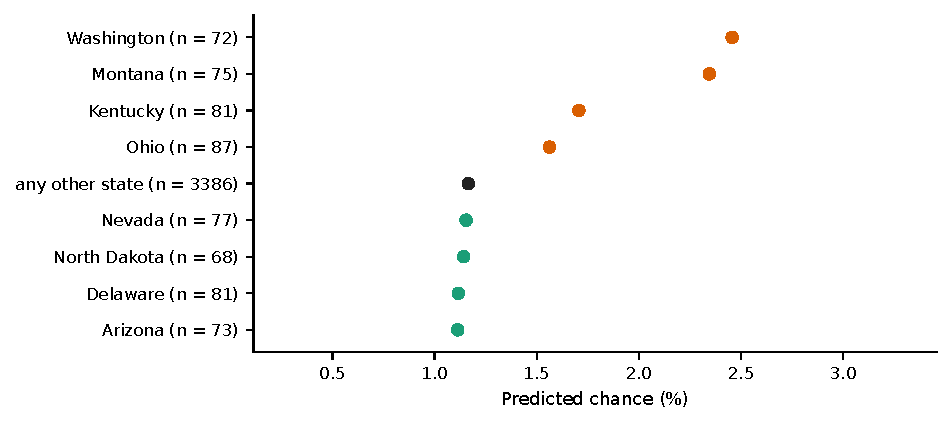
\includegraphics[width=\linewidth,height=0.88\textheight,keepaspectratio]{figures/churn100-s2-c2/ann_95-categories-C125.pdf}
\caption{State units: The predicted value for the typical case at each level, through this part (n = training customers; grey: fewer than 20).}
\label{fig:churn100s2c2:plot-ann95-0}
\end{figure}
\begin{figure}[H]\centering
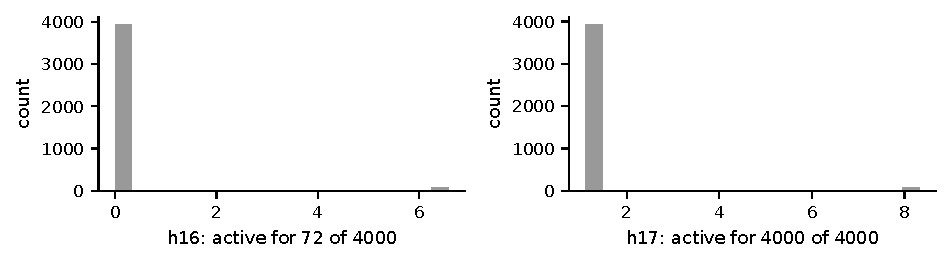
\includegraphics[width=\linewidth,height=0.88\textheight,keepaspectratio]{figures/churn100-s2-c2/ann_95-units.pdf}
\caption{State units: This part's hidden units: each unit's output against its main numeric input (top) and how often it is active (bottom).}
\label{fig:churn100s2c2:plot-ann95-1}
\end{figure}
\par\smallskip\noindent{\small Technical detail: \ref{tech:ann95}.\par}
\subsubsection{Area-code unit}\label{rd:ann94}
\noindent{\footnotesize Part of: The whole model (\ref{rd:ann97}).\par}
\noindent{\small Figure~\ref{fig:churn100s2c2:parts-ann94} shows what feeds this part; Figure~\ref{fig:churn100s2c2:units-ann94} its units and every connection into them (dashed boxes: connections from or to other parts, drawn in their own sections).\par}
\begin{figure}[H]\centering
\resizebox{!}{\ifdim\height>0.5\textheight 0.5\textheight\else\height\fi}{%
\resizebox{\ifdim\width>\linewidth\linewidth\else\width\fi}{!}{%
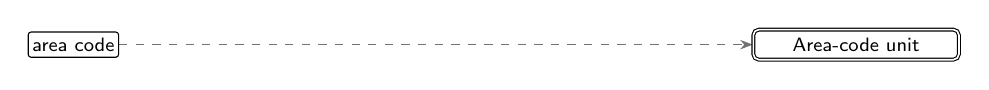
\begin{tikzpicture}[
  font=\sffamily\scriptsize, >={Stealth[length=1.6mm]},
  inp/.style={draw, rounded corners=1pt, fill=white, inner sep=1.5pt, minimum height=3.2mm, anchor=east},
  abox/.style={draw, thick, rounded corners=2pt, align=center, inner sep=3pt, minimum height=6mm, text width=42mm},
  outp/.style={draw, double, rounded corners=2pt, fill=white, align=center, inner sep=3pt, text width=24mm},
  agg/.style={draw=black!55},
]
\node[inp] (i0) at (0,-0.0) {area code};
\node[outp] (out) at (9.36,0) {Area-code unit};
\begin{scope}[on background layer]
\draw[->, agg, thin, dashed] (i0.east) -- (out.west);
\end{scope}
\end{tikzpicture}}}%
\caption{Area-code unit: what feeds it, one level down.}
\label{fig:churn100s2c2:parts-ann94}
\end{figure}
\begin{figure}[H]\centering
\resizebox{\ifdim\width>\linewidth\linewidth\else\width\fi}{!}{%
\definecolor{netup}{HTML}{D95F02}\definecolor{netdown}{HTML}{1B9E77}\definecolor{netmixed}{HTML}{7F7F7F}%
\begin{tikzpicture}[
  font=\sffamily\scriptsize, >={Stealth[length=1.4mm]},
  inp/.style={draw, circle, fill=white, minimum size=3.2mm, inner sep=0pt},
  hid/.style={draw, circle, fill=white, minimum size=5.2mm, inner sep=0.5pt, font=\sffamily\tiny},
  exitbox/.style={draw, thick, rectangle, fill=white, align=center, text width=17mm, minimum height=5mm, inner sep=1.5pt, font=\sffamily\tiny},
  sumbox/.style={draw, thick, dashed, rectangle, fill=white, align=center, text width=17mm, minimum height=5mm, inner sep=1.5pt, font=\sffamily\tiny},
  outp/.style={draw, thick, regular polygon, regular polygon sides=6, fill=white, minimum size=10mm, inner sep=0pt, font=\sffamily\tiny, align=center},
  stub/.style={draw, dashed, rounded corners=2pt, fill=white, align=center, inner sep=2pt, font=\sffamily\tiny, text width=15mm},
  inlab/.style={font=\sffamily\tiny, align=center, text width=15mm, inner sep=1pt, fill=white, fill opacity=0.8, text opacity=1},
  wpos/.style={draw=NavyBlue}, wneg/.style={draw=BrickRed}, wagg/.style={draw=black!45, line width=1.2pt},
  wmix/.style={draw=Plum},
]
\node[hid] (n161) at (2.55,1.9) {h1};
\node[hid] (n14653) at (1.05,1.9) {h21};
\node[inp, draw=netup, very thick] (ninxxareaxcodex415) at (2.7,0.0) {};
\path (ninxxareaxcodex415.south) node[inlab, anchor=north] (labninxxareaxcodex415) {area code 415 $\uparrow$};
\node[inp, draw=netdown, very thick] (ninxxareaxcodex408) at (0.9,0.0) {};
\path (ninxxareaxcodex408.south) node[inlab, anchor=north] (labninxxareaxcodex408) {area code 408 $\downarrow$};
\node[stub] (ntoxxthexmodelxoutput) at (1.8,3.45) {to the model output};
\begin{scope}[on background layer]
\node[fit=(n161) (n14653) , inner sep=8pt, rounded corners=5pt, fill=Cerulean!10, draw=Cerulean!45] (clu0) {};
\draw[->, wpos, line width=0.45pt] (ninxxareaxcodex415) -- (n161);
\draw[->, wneg, line width=0.44pt] (ninxxareaxcodex408) -- (n14653);
\draw[->, wpos, line width=0.27pt] (n161) -- (ntoxxthexmodelxoutput);
\draw[->, wneg, line width=0.34pt] (n14653) -- (ntoxxthexmodelxoutput);
\end{scope}
\node[font=\sffamily\scriptsize\bfseries, text=Cerulean!55!black, anchor=south west, inner sep=1pt, fill=white, fill opacity=0.85, text opacity=1] at (clu0.north west) {Area-code unit};
\end{tikzpicture}}%
\caption{Area-code unit: its units and every connection into them. Blue: positive weight (raises the score); red: negative weight (lowers it); thicker: larger weight. Orange outline and up arrow: raises the final prediction; teal and down arrow: lowers it; grey and double arrow: depends.}
\label{fig:churn100s2c2:units-ann94}
\end{figure}
\paragraph{Hypothesis.} This part reads the area code and barely changes the predictions.\,{\scriptsize\textcolor{NavyBlue}{[C137]}}
\paragraph{Evidence.} Through it, a typical customer's chance stays at about 1\% in area codes 408 and 510, as in area code 415.\,{\scriptsize\textcolor{NavyBlue}{[C134, C135]}} Switching it off changes the predictions by at most half a point.\,{\scriptsize\textcolor{NavyBlue}{[C137]}} Its formula reproduces the part exactly on all 4000 training customers.\,{\scriptsize\textcolor{NavyBlue}{[C138]}}
\par\noindent{\small Evidence plots: Figure~\ref{fig:churn100s2c2:plot-ann94-0}, Figure~\ref{fig:churn100s2c2:plot-ann94-1}.\par}
\begin{figure}[H]\centering
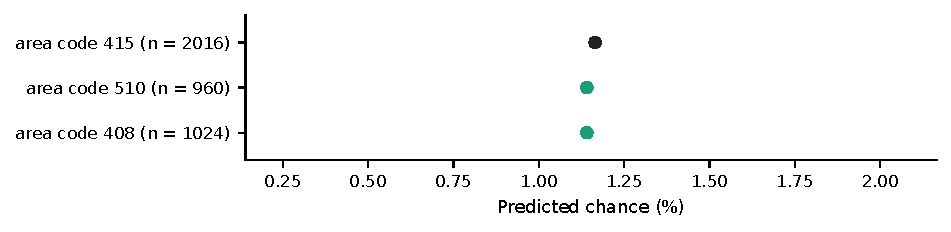
\includegraphics[width=\linewidth,height=0.88\textheight,keepaspectratio]{figures/churn100-s2-c2/ann_94-categories-small.pdf}
\caption{Area-code unit: The predicted value for the typical case at each level, through this part (n = training customers; grey: fewer than 20).}
\label{fig:churn100s2c2:plot-ann94-0}
\end{figure}
\begin{figure}[H]\centering
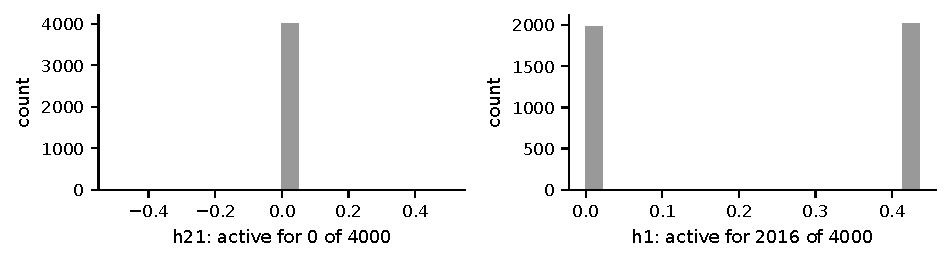
\includegraphics[width=\linewidth,height=0.88\textheight,keepaspectratio]{figures/churn100-s2-c2/ann_94-units.pdf}
\caption{Area-code unit: This part's hidden units: each unit's output against its main numeric input (top) and how often it is active (bottom).}
\label{fig:churn100s2c2:plot-ann94-1}
\end{figure}
\par\smallskip\noindent{\small Technical detail: \ref{tech:ann94}.\par}
\subsubsection{Small Utah unit}\label{rd:ann93}
\noindent{\footnotesize Part of: The whole model (\ref{rd:ann97}).\par}
\noindent{\small Figure~\ref{fig:churn100s2c2:parts-ann93} shows what feeds this part; Figure~\ref{fig:churn100s2c2:units-ann93} its units and every connection into them (dashed boxes: connections from or to other parts, drawn in their own sections).\par}
\begin{figure}[H]\centering
\resizebox{!}{\ifdim\height>0.5\textheight 0.5\textheight\else\height\fi}{%
\resizebox{\ifdim\width>\linewidth\linewidth\else\width\fi}{!}{%
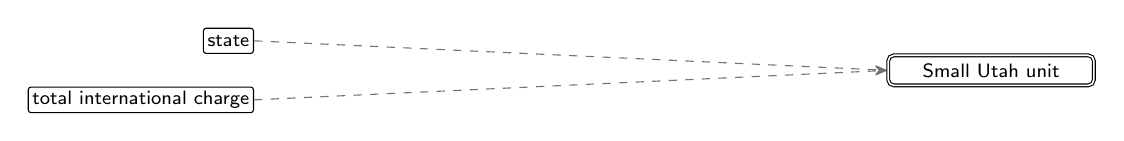
\begin{tikzpicture}[
  font=\sffamily\scriptsize, >={Stealth[length=1.6mm]},
  inp/.style={draw, rounded corners=1pt, fill=white, inner sep=1.5pt, minimum height=3.2mm, anchor=east},
  abox/.style={draw, thick, rounded corners=2pt, align=center, inner sep=3pt, minimum height=6mm, text width=42mm},
  outp/.style={draw, double, rounded corners=2pt, fill=white, align=center, inner sep=3pt, text width=24mm},
  agg/.style={draw=black!55},
]
\node[inp] (i0) at (0,0.375) {state};
\node[inp] (i1) at (0,-0.375) {total international charge};
\node[outp] (out) at (9.36,0) {Small Utah unit};
\begin{scope}[on background layer]
\draw[->, agg, thin, dashed] (i0.east) -- (out.west);
\draw[->, agg, thin, dashed] (i1.east) -- (out.west);
\end{scope}
\end{tikzpicture}}}%
\caption{Small Utah unit: what feeds it, one level down.}
\label{fig:churn100s2c2:parts-ann93}
\end{figure}
\begin{figure}[H]\centering
\resizebox{\ifdim\width>\linewidth\linewidth\else\width\fi}{!}{%
\definecolor{netup}{HTML}{D95F02}\definecolor{netdown}{HTML}{1B9E77}\definecolor{netmixed}{HTML}{7F7F7F}%
\begin{tikzpicture}[
  font=\sffamily\scriptsize, >={Stealth[length=1.4mm]},
  inp/.style={draw, circle, fill=white, minimum size=3.2mm, inner sep=0pt},
  hid/.style={draw, circle, fill=white, minimum size=5.2mm, inner sep=0.5pt, font=\sffamily\tiny},
  exitbox/.style={draw, thick, rectangle, fill=white, align=center, text width=17mm, minimum height=5mm, inner sep=1.5pt, font=\sffamily\tiny},
  sumbox/.style={draw, thick, dashed, rectangle, fill=white, align=center, text width=17mm, minimum height=5mm, inner sep=1.5pt, font=\sffamily\tiny},
  outp/.style={draw, thick, regular polygon, regular polygon sides=6, fill=white, minimum size=10mm, inner sep=0pt, font=\sffamily\tiny, align=center},
  stub/.style={draw, dashed, rounded corners=2pt, fill=white, align=center, inner sep=2pt, font=\sffamily\tiny, text width=15mm},
  inlab/.style={font=\sffamily\tiny, align=center, text width=15mm, inner sep=1pt, fill=white, fill opacity=0.8, text opacity=1},
  wpos/.style={draw=NavyBlue}, wneg/.style={draw=BrickRed}, wagg/.style={draw=black!45, line width=1.2pt},
  wmix/.style={draw=Plum},
]
\node[exitbox] (n252) at (1.8,1.9) {Small Utah unit $\uparrow$};
\node[inp, draw=netmixed, very thick] (ngrpxxstate) at (0.9,0.0) {};
\path (ngrpxxstate.south) node[inlab, anchor=north] (labngrpxxstate) {state (26 of 51 used) $\updownarrow$};
\node[inp, draw=netdown, very thick] (ninxxtotalxintlxcharge) at (2.7,0.0) {};
\path (ninxxtotalxintlxcharge.south) node[inlab, anchor=north] (labninxxtotalxintlxcharge) {total international charge $\downarrow$};
\node[stub] (ntoxxthexmodelxoutput) at (1.8,3.45) {to the model output};
\begin{scope}[on background layer]
\node[fit=(n252) , inner sep=8pt, rounded corners=5pt, fill=Mahogany!10, draw=Mahogany!45] (clu0) {};
\draw[->, wneg, line width=0.55pt] (ninxxtotalxintlxcharge) -- (n252);
\draw[->, wpos, line width=0.25pt] (n252) -- (ntoxxthexmodelxoutput);
\draw[->, wpos, line width=0.40pt] (ngrpxxstate) -- node[pos=0.8, sloped, above, font=\sffamily\tiny, inner sep=1pt, fill=white, fill opacity=0.8, text opacity=1] {+0.43} (n252);
\end{scope}
\node[font=\sffamily\scriptsize\bfseries, text=Mahogany!55!black, anchor=south west, inner sep=1pt, fill=white, fill opacity=0.85, text opacity=1] at (clu0.north west) {Small Utah unit};
\end{tikzpicture}}%
\caption{Small Utah unit: its units and every connection into them. Blue: positive weight (raises the score); red: negative weight (lowers it); thicker: larger weight. Orange outline and up arrow: raises the final prediction; teal and down arrow: lowers it; grey and double arrow: depends.}
\label{fig:churn100s2c2:units-ann93}
\end{figure}
\paragraph{Hypothesis.} This small part reads the international charge and being in Utah, and barely changes the predictions.\,{\scriptsize\textcolor{NavyBlue}{[C144]}}
\paragraph{Evidence.} Through it, the international charge barely changes the chance, which stays at about 1\% for the typical customer it acts on.\,{\scriptsize\textcolor{NavyBlue}{[C139]}} Switching it off changes the predictions by at most 0.2 points.\,{\scriptsize\textcolor{NavyBlue}{[C144]}} Its formula reproduces the part exactly on all 4000 training customers.\,{\scriptsize\textcolor{NavyBlue}{[C145]}}
\par\noindent{\small Evidence plots: Figure~\ref{fig:churn100s2c2:plot-ann93-0}, Figure~\ref{fig:churn100s2c2:plot-ann93-1}, Figure~\ref{fig:churn100s2c2:plot-ann93-2}, Figure~\ref{fig:churn100s2c2:plot-ann93-3}.\par}
\par\noindent{\small Figure~\ref{fig:churn100s2c2:plot-ann93-2} shows this part's own output, unit h2.\par}
\begin{figure}[H]\centering
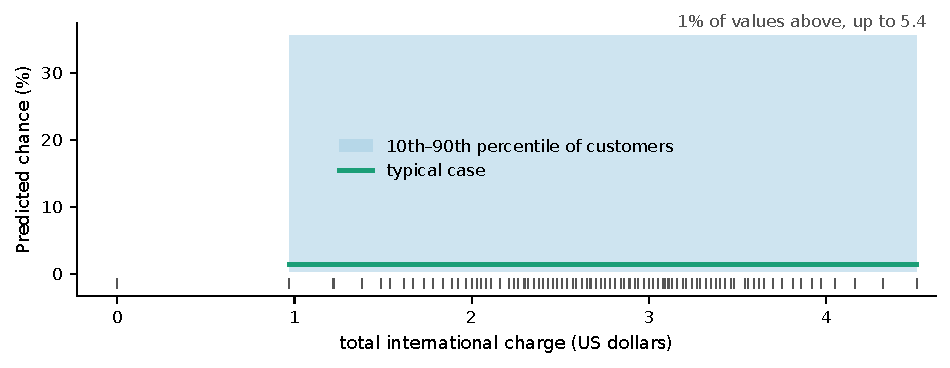
\includegraphics[width=\linewidth,height=0.88\textheight,keepaspectratio]{figures/churn100-s2-c2/ann_93-response.pdf}
\caption{Small Utah unit: Response curves through this part: the typical case (bold), the 10th to 90th percentile of individual customers (band), the fold or step point (dashed) with its spread across them (grey), and the observed values (ticks).}
\label{fig:churn100s2c2:plot-ann93-0}
\end{figure}
\begin{figure}[H]\centering
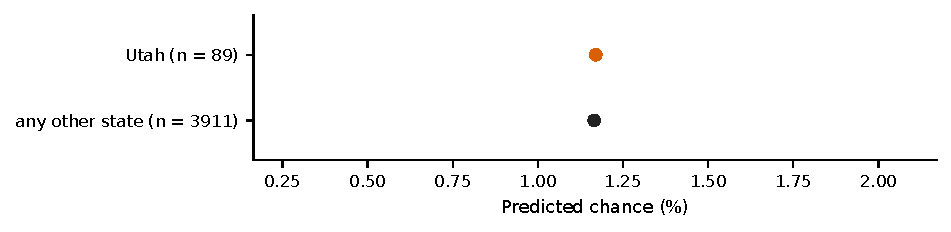
\includegraphics[width=\linewidth,height=0.88\textheight,keepaspectratio]{figures/churn100-s2-c2/ann_93-categories-small.pdf}
\caption{Small Utah unit: The predicted value for the typical case at each level, through this part (n = training customers; grey: fewer than 20).}
\label{fig:churn100s2c2:plot-ann93-1}
\end{figure}
\begin{figure}[H]\centering
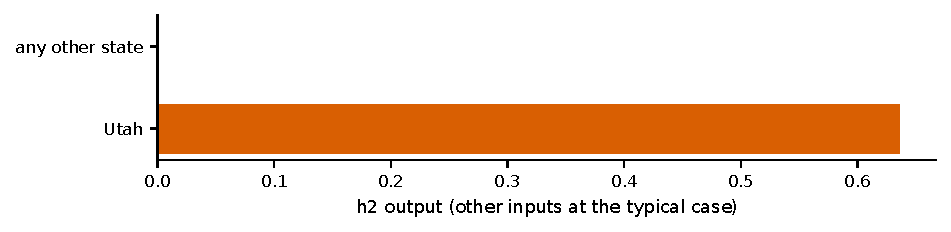
\includegraphics[width=\linewidth,height=0.88\textheight,keepaspectratio]{figures/churn100-s2-c2/ann_93-partial-252.pdf}
\caption{Small Utah unit: This part's own output, unit h2 (the output of 'Small Utah unit'), on its own scale (its activation), with every other input at the typical case; it is active for 100 of 4000. Its output for each combination of the levels it reads.}
\label{fig:churn100s2c2:plot-ann93-2}
\end{figure}
\begin{figure}[H]\centering
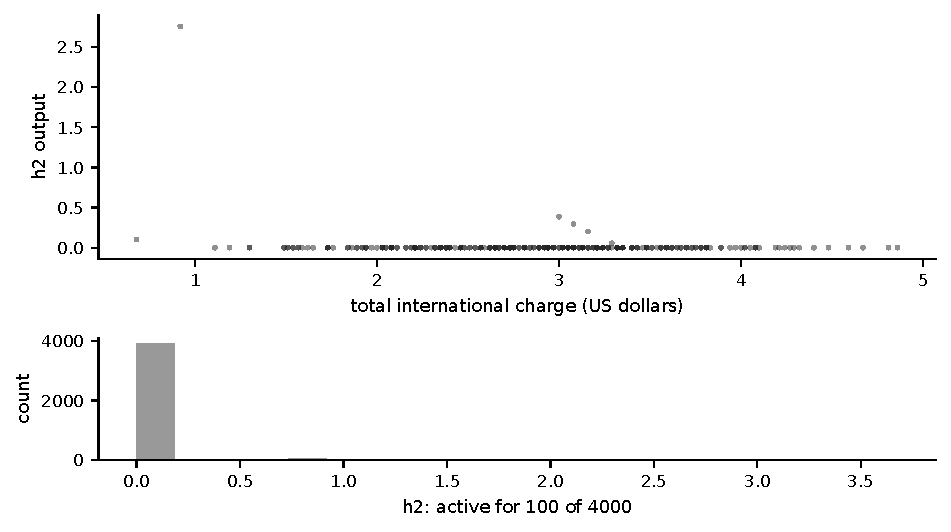
\includegraphics[width=\linewidth,height=0.88\textheight,keepaspectratio]{figures/churn100-s2-c2/ann_93-units.pdf}
\caption{Small Utah unit: This part's hidden units: each unit's output against its main numeric input (top) and how often it is active (bottom).}
\label{fig:churn100s2c2:plot-ann93-3}
\end{figure}
\par\smallskip\noindent{\small Technical detail: \ref{tech:ann93}.\par}
\subsection{Not supported by the model}
\begin{itemize}\setlength\itemsep{0pt}\small
\item C002: direction claim about total daytime minutes in the whole model: not supported by the model (14\% of patients have the opposite sign (allowed: 10\%)).
\item C017: direction claim about total evening charge in the whole model: not supported by the model (52\% of patients have the opposite sign (allowed: 10\%)).
\item C026: direction claim about state in the whole model: not supported by the model (53\% of patients have the opposite sign (allowed: 10\%)).
\item C136: subgroup claim about area code in part ann\_\allowbreak{}94: not supported by the model (its effect is negligible).
\item C141: interaction claim about total international charge and state in part ann\_\allowbreak{}93: not supported by the model (the group difference is below 0.1 log-odds; the part's own counterfactual difference has the opposite sign).
\item C142: threshold claim about total international charge in part ann\_\allowbreak{}93: not supported by the model (the fold changes the curve by only 0.037 log-odds compared with a straight line (needed 0.1); the effect past the fold is too small or not consistent across patients).
\item C143: subgroup claim about state and total international charge in part ann\_\allowbreak{}93: not supported by the model (its effect is negligible).
\item C146: boundary claim about number of calls to customer service and total daytime minutes in part ann\_\allowbreak{}96: not supported by the model (no switch-on line could be traced on the first map to check against the data; no switch-on boundary in the observed range).
\item C147: boundary claim about total daytime minutes and number of calls to customer service in part ann\_\allowbreak{}90: not supported by the model (no switch-on line could be traced on the first map to check against the data; no switch-on boundary in the observed range).
\end{itemize}
\clearpage\section*{Technical detail: churn100-s2-c2}
\addcontentsline{toc}{section}{Technical detail: churn100-s2-c2}
\noindent{\small The record behind each part: the original hypothesis, the closed form, and every claim with its estimate (log-odds and odds ratio), range across patients, n and test check.\par}
\renewcommand{\thesubsection}{T.\arabic{subsection}}\setcounter{subsection}{0}
\subsection{The whole model}\label{tech:ann97}
\noindent{\footnotesize Annotation ann\_\allowbreak{}97 (churn\_\allowbreak{}logit). Reads: state, account length, area code, international calling plan, voice-mail plan, number of voice-mail messages, total daytime minutes, total daytime calls, total daytime charge, total evening minutes, total evening calls, total evening charge, total night-time minutes, total night-time calls, total night-time charge, total international minutes, total international calls, total international charge, number of calls to customer service.\par}
\paragraph{Original hypothesis (unchanged).} Root: logit P(churn) = -1.15 + linear\_\allowbreak{}backbone + service\_\allowbreak{}call\_\allowbreak{}nonlinear (identity\_\allowbreak{}svc) - 0.89*1133 - 1.00*4051 (voicemail\_\allowbreak{}chain) + state\_\allowbreak{}offsets + 0.05*161 - 0.25*14653 (area codes, 14653 dead) + 0.007*252, purely additive in the logit; the sigmoid is the only coupling. 30 inputs are unconnected (international minutes, night charge, night calls, evening calls, day charge and 25 state indicators) and have zero effect. Train AUC 0.8944, accuracy 0.896. Performance sources (train): all children replaced by least-squares linear fits gives AUC 0.8314 (an L2 logistic regression refit on all 71 inputs gets 0.8433); restoring csc\_\allowbreak{}usage\_\allowbreak{}gate alone gives 0.8917, csc\_\allowbreak{}hinge alone 0.8462, the others 0.8314 (exactly or nearly linear). So the gain over linear comes from the service-call x low-usage gate. Rare-category switches: state:11 -1.93 logit (73 rows, empirical -1.35); state:47 +1.47 mean (72 rows, empirical +0.92; direct +1.39, +0.76 via 10332, but it switches off 1264, down to -1.38 for some); state:4 +1.34 (41 rows, +0.80); state:0 -1.13 mean, down to -5.0 (56 rows, -0.76; switches off 2796 in the gate); state:26 +1.09 (75 rows, +0.50; via direct + state offsets); state:43 +0.88 (95 rows, +0.48); state:45 -0.71 (91 rows, -0.85).
\paragraph{Closed form.} Read through its parts (their formulas are in their own sections).
\paragraph{Split inputs.} To annotate the parts, the explanation split these inputs into copies (a refactoring step that does not change what the model computes); the diagrams draw each input once: customer-service calls (2 copies); total daytime minutes (2 copies); total evening charge (2 copies); total international charge (3 copies); a voice-mail plan (2 copies).
\paragraph{State: every level the model reads.} Whole-model change in the predicted chance for a typical customer when only the state changes from the reference; n = training customers in that level.\par\smallskip
{\scriptsize\rowcolors{2}{black!6}{white}
\begin{longtable}{@{}lllrlc@{}}
\toprule\rowcolor{white}
Claim & From & To & n & Chance & OK \\
\midrule\endhead
\bottomrule\endfoot
C003 & West Virginia & Washington & 72 & 1\% to 9\% & \textcolor{OliveGreen}{yes} \\
C004 & West Virginia & California & 41 & 1\% to 5\% & \textcolor{OliveGreen}{yes} \\
C006 & West Virginia & Montana & 75 & 1\% to 4\% & \textcolor{OliveGreen}{yes} \\
C007 & West Virginia & Texas & 95 & 1\% to 3\% & \textcolor{OliveGreen}{yes} \\
C013 & West Virginia & South Carolina & 66 & 1\% to 2\% & \textcolor{OliveGreen}{yes} \\
C014 & West Virginia & Maryland & 82 & 1\% to 2\% & \textcolor{OliveGreen}{yes} \\
C016 & West Virginia & Nevada & 77 & 1\% to 2\% & \textcolor{OliveGreen}{yes} \\
C018 & West Virginia & Kentucky & 81 & 1\% to 2\% & \textcolor{OliveGreen}{yes} \\
C019 & West Virginia & Massachusetts & 86 & 1\% to 2\% & \textcolor{OliveGreen}{yes} \\
C021 & West Virginia & Ohio & 87 & 1\% to 2\% & \textcolor{OliveGreen}{yes} \\
C022 & West Virginia & Minnesota & 100 & 1\% to 2\% & \textcolor{OliveGreen}{yes} \\
C024 & West Virginia & Oregon & 84 & 1\% to 2\% & \textcolor{OliveGreen}{yes} \\
C030 & West Virginia & Utah & 89 & 1\% to 1\% & \textcolor{OliveGreen}{yes} \\
C031 & West Virginia & state other than Alaska, Hawaii, Indiana, Kentucky, Massa... & 1947 & 1\% to 1\% & \textcolor{OliveGreen}{yes} \\
C034 & West Virginia & Arizona & 73 & 1\% to 1\% & \textcolor{OliveGreen}{yes} \\
C035 & West Virginia & Oklahoma & 79 & 1\% to 1\% & \textcolor{OliveGreen}{yes} \\
C037 & West Virginia & Delaware & 81 & 1\% to 1\% & \textcolor{OliveGreen}{yes} \\
C039 & West Virginia & Indiana & 82 & 1\% to 1\% & \textcolor{OliveGreen}{yes} \\
C036 & West Virginia & North Carolina & 74 & 1\% to 1\% & \textcolor{OliveGreen}{yes} \\
C033 & West Virginia & North Dakota & 68 & 1\% to 1\% & \textcolor{OliveGreen}{yes} \\
C029 & West Virginia & Washington DC & 73 & 1\% to 1\% & \textcolor{OliveGreen}{yes} \\
C028 & West Virginia & Missouri & 80 & 1\% to 1\% & \textcolor{OliveGreen}{yes} \\
C026 & West Virginia & South Dakota & 66 & 1\% to 1\% & \textcolor{BrickRed}{no} \\
C023 & West Virginia & Alaska & 56 & 1\% to 1\% & \textcolor{OliveGreen}{yes} \\
C020 & West Virginia & Virginia & 91 & 1\% to 1\% & \textcolor{OliveGreen}{yes} \\
C012 & West Virginia & Hawaii & 73 & 1\% to $<$1\% & \textcolor{OliveGreen}{yes} \\
\end{longtable}}
\paragraph{Evidence table} (next page, landscape).
\begin{landscape}
{\scriptsize\setlength{\tabcolsep}{3pt}\renewcommand{\arraystretch}{1.15}
\rowcolors{2}{black!6}{white}
\begin{longtable}{@{}l>{\raggedright\arraybackslash}p{0.36\linewidth}>{\raggedright\arraybackslash}p{0.14\linewidth}rrr>{\raggedright\arraybackslash}p{0.06\linewidth}>{\raggedright\arraybackslash}p{0.17\linewidth}c@{}}
\toprule\rowcolor{white}
ID & What is checked & Risk, typical patient & Log-odds & OR & Range (p10--p90) & n & Test check & OK \\
\midrule\endfirsthead
\toprule\rowcolor{white}
ID & What is checked & Risk, typical patient & Log-odds & OR & Range (p10--p90) & n & Test check & OK \\
\midrule\endhead
\bottomrule\endfoot
C001 & direction: international calling plan: no international plan to an international plan (whole model) \newline{\itshape shape: categorical; highest to lowest: an international plan, no international plan} & 1\% to 14\% & 2.60 & 13.5 & 2.60 to 2.60 & 3620, 380 & agrees; AUC gain 0.056 [0.032, 0.082] & \textcolor{OliveGreen}{yes} \\
C002 & direction: total daytime minutes: 112 minutes to 249 minutes (whole model) \newline{\itshape shape: dip at 154 minutes; 99\% of patients same; verified; risk saturates near 0\%} & 1\% to 11\% & 1.64 & 5.16 & -0.45 to 3.10 & 4000 & agrees; AUC gain 0.081 [0.053, 0.112] & \textcolor{BrickRed}{no} \\
C003 & direction: state: West Virginia to Washington (whole model) \newline{\itshape shape: categorical; highest to lowest: Washington, California, Montana, Texas, South Carolina, Maryland ...} & 1\% to 9\% & 1.66 & 5.24 & 0.76 to 2.22 & 122, 72 & disagrees; AUC gain -0.002 [-0.012, 0.008] & \textcolor{OliveGreen}{yes} \\
C004 & direction: state: West Virginia to California (whole model) \newline{\itshape shape: categorical; highest to lowest: Washington, California, Montana, Texas, South Carolina, Maryland ...} & 1\% to 5\% & 1.42 & 4.15 & 1.42 to 1.42 & 122, 41 & disagrees; AUC gain -0.002 [-0.012, 0.008] & \textcolor{OliveGreen}{yes} \\
C005 & direction: voice-mail messages: 0 messages to 32 messages (whole model) \newline{\itshape shape: steady; 100\% of patients same; verified; risk saturates near 0\%} & 1\% to 4\% & 1.36 & 3.91 & 1.36 to 1.36 & 4000 & agrees; AUC gain 0.018 [0.006, 0.030] & \textcolor{OliveGreen}{yes} \\
C006 & direction: state: West Virginia to Montana (whole model) \newline{\itshape shape: categorical; highest to lowest: Washington, California, Montana, Texas, South Carolina, Maryland ...} & 1\% to 4\% & 1.17 & 3.23 & 1.17 to 1.17 & 122, 75 & disagrees; AUC gain -0.002 [-0.012, 0.008] & \textcolor{OliveGreen}{yes} \\
C007 & direction: state: West Virginia to Texas (whole model) \newline{\itshape shape: categorical; highest to lowest: Washington, California, Montana, Texas, South Carolina, Maryland ...} & 1\% to 3\% & 0.96 & 2.60 & 0.96 to 0.96 & 122, 95 & disagrees; AUC gain -0.002 [-0.012, 0.008] & \textcolor{OliveGreen}{yes} \\
C008 & direction: total evening minutes: 138 minutes to 266 minutes (whole model) \newline{\itshape shape: steady; 100\% of patients same; verified; risk saturates near 0\%} & 1\% to 2\% & 1.26 & 3.54 & 1.26 to 1.26 & 4000 & agrees; AUC gain 0.014 [0.004, 0.024] & \textcolor{OliveGreen}{yes} \\
C009 & direction: total international charge: 1.84 US dollars to 3.70 US dollars (whole model) \newline{\itshape shape: accelerating; 93\% of patients same; verified; risk saturates near 0\%} & 1\% to 2\% & 0.61 & 1.85 & 0.15 to 0.79 & 4000 & unclear; AUC gain 0.006 [-4e-05, 0.012] & \textcolor{OliveGreen}{yes} \\
C010 & direction: voice-mail plan: no voice-mail plan to a voice-mail plan (whole model) \newline{\itshape shape: categorical; highest to lowest: no voice-mail plan, a voice-mail plan} & 1\% to $<$1\% & -3.26 & 0.04 & -3.26 to -3.26 & 2939, 1061 & agrees; AUC gain 0.024 [0.0005, 0.047] & \textcolor{OliveGreen}{yes} \\
C011 & direction: customer-service calls: 0 calls to 3 calls (whole model) \newline{\itshape shape: accelerating; 94\% of patients same; verified; risk saturates near 0\%} & 1\% to 2\% & 0.94 & 2.56 & 0.00 to 2.43 & 4000 & agrees; AUC gain 0.095 [0.059, 0.134] & \textcolor{OliveGreen}{yes} \\
C012 & direction: state: West Virginia to Hawaii (whole model) \newline{\itshape shape: categorical; highest to lowest: Washington, California, Montana, Texas, South Carolina, Maryland ...} & 1\% to $<$1\% & -1.86 & 0.16 & -1.86 to -1.86 & 122, 73 & disagrees; AUC gain -0.002 [-0.012, 0.008] & \textcolor{OliveGreen}{yes} \\
C013 & direction: state: West Virginia to South Carolina (whole model) \newline{\itshape shape: categorical; highest to lowest: Washington, California, Montana, Texas, South Carolina, Maryland ...} & 1\% to 2\% & 0.61 & 1.84 & 0.61 to 0.61 & 122, 66 & disagrees; AUC gain -0.002 [-0.012, 0.008] & \textcolor{OliveGreen}{yes} \\
C014 & direction: state: West Virginia to Maryland (whole model) \newline{\itshape shape: categorical; highest to lowest: Washington, California, Montana, Texas, South Carolina, Maryland ...} & 1\% to 2\% & 0.60 & 1.83 & 0.60 to 0.60 & 122, 82 & disagrees; AUC gain -0.002 [-0.012, 0.008] & \textcolor{OliveGreen}{yes} \\
C015 & direction: total night-time minutes: 136 minutes to 264 minutes (whole model) \newline{\itshape shape: steady; 100\% of patients same; verified; risk saturates near 0\%} & 1\% to 2\% & 0.70 & 2.01 & 0.70 to 0.70 & 4000 & unclear; AUC gain 0.004 [-0.0008, 0.008] & \textcolor{OliveGreen}{yes} \\
C016 & direction: state: West Virginia to Nevada (whole model) \newline{\itshape shape: categorical; highest to lowest: Washington, California, Montana, Texas, South Carolina, Maryland ...} & 1\% to 2\% & 0.52 & 1.69 & 0.52 to 0.52 & 122, 77 & disagrees; AUC gain -0.002 [-0.012, 0.008] & \textcolor{OliveGreen}{yes} \\
C017 & direction: total evening charge: 11.76 US dollars to 22.57 US dollars (whole model) \newline{\itshape shape: dip at 12.96 US dollars; 71\% of patients same; fallback; risk saturates near 0\%} & 1\% to 2\% & -0.20 & 0.82 & -1.79 to 0.87 & 4000 & unclear; AUC gain 0.005 [-0.005, 0.015] & \textcolor{BrickRed}{no} \\
C018 & direction: state: West Virginia to Kentucky (whole model) \newline{\itshape shape: categorical; highest to lowest: Washington, California, Montana, Texas, South Carolina, Maryland ...} & 1\% to 2\% & 0.47 & 1.59 & 0.47 to 0.47 & 122, 81 & disagrees; AUC gain -0.002 [-0.012, 0.008] & \textcolor{OliveGreen}{yes} \\
C019 & direction: state: West Virginia to Massachusetts (whole model) \newline{\itshape shape: categorical; highest to lowest: Washington, California, Montana, Texas, South Carolina, Maryland ...} & 1\% to 2\% & 0.42 & 1.52 & 0.42 to 0.42 & 122, 86 & disagrees; AUC gain -0.002 [-0.012, 0.008] & \textcolor{OliveGreen}{yes} \\
C020 & direction: state: West Virginia to Virginia (whole model) \newline{\itshape shape: categorical; highest to lowest: Washington, California, Montana, Texas, South Carolina, Maryland ...} & 1\% to 1\% & -0.63 & 0.53 & -0.63 to -0.63 & 122, 91 & disagrees; AUC gain -0.002 [-0.012, 0.008] & \textcolor{OliveGreen}{yes} \\
C021 & direction: state: West Virginia to Ohio (whole model) \newline{\itshape shape: categorical; highest to lowest: Washington, California, Montana, Texas, South Carolina, Maryland ...} & 1\% to 2\% & 0.38 & 1.46 & 0.38 to 0.38 & 122, 87 & disagrees; AUC gain -0.002 [-0.012, 0.008] & \textcolor{OliveGreen}{yes} \\
C022 & direction: state: West Virginia to Minnesota (whole model) \newline{\itshape shape: categorical; highest to lowest: Washington, California, Montana, Texas, South Carolina, Maryland ...} & 1\% to 2\% & 0.36 & 1.44 & 0.36 to 0.36 & 122, 100 & disagrees; AUC gain -0.002 [-0.012, 0.008] & \textcolor{OliveGreen}{yes} \\
C023 & direction: state: West Virginia to Alaska (whole model) \newline{\itshape shape: categorical; highest to lowest: Washington, California, Montana, Texas, South Carolina, Maryland ...} & 1\% to 1\% & -1.01 & 0.36 & -2.44 to -0.52 & 122, 56 & disagrees; AUC gain -0.002 [-0.012, 0.008] & \textcolor{OliveGreen}{yes} \\
C024 & direction: state: West Virginia to Oregon (whole model) \newline{\itshape shape: categorical; highest to lowest: Washington, California, Montana, Texas, South Carolina, Maryland ...} & 1\% to 2\% & 0.31 & 1.36 & 0.31 to 0.31 & 122, 84 & disagrees; AUC gain -0.002 [-0.012, 0.008] & \textcolor{OliveGreen}{yes} \\
C025 & direction: total international calls: 2 calls to 8 calls (whole model) \newline{\itshape shape: steady (equal steps); 100\% of patients same; verified; risk saturates near 0\%} & 1\% to 1\% & -0.38 & 0.68 & -0.38 to -0.38 & 4000 & unclear; AUC gain 0.0005 [-0.002, 0.003] & \textcolor{OliveGreen}{yes} \\
C026 & direction: state: West Virginia to South Dakota (whole model) \newline{\itshape shape: categorical; highest to lowest: Washington, California, Montana, Texas, South Carolina, Maryland ...} & 1\% to 1\% & 0.06 & 1.07 & -0.51 to 0.78 & 122, 66 & disagrees; AUC gain -0.002 [-0.012, 0.008] & \textcolor{BrickRed}{no} \\
C027 & direction: account length: 48 to 152 (whole model) \newline{\itshape shape: steady; 100\% of patients same; verified; risk saturates near 0\%} & 1\% to 1\% & 0.33 & 1.39 & 0.33 to 0.33 & 4000 & disagrees; AUC gain -0.001 [-0.004, 0.0006] & \textcolor{OliveGreen}{yes} \\
C028 & direction: state: West Virginia to Missouri (whole model) \newline{\itshape shape: categorical; highest to lowest: Washington, California, Montana, Texas, South Carolina, Maryland ...} & 1\% to 1\% & -0.17 & 0.85 & -0.17 to -0.17 & 122, 80 & disagrees; AUC gain -0.002 [-0.012, 0.008] & \textcolor{OliveGreen}{yes} \\
C029 & direction: state: West Virginia to Washington DC (whole model) \newline{\itshape shape: categorical; highest to lowest: Washington, California, Montana, Texas, South Carolina, Maryland ...} & 1\% to 1\% & -0.12 & 0.89 & -0.12 to -0.12 & 122, 73 & disagrees; AUC gain -0.002 [-0.012, 0.008] & \textcolor{OliveGreen}{yes} \\
C030 & direction: state: West Virginia to Utah (whole model) \newline{\itshape shape: categorical; highest to lowest: Washington, California, Montana, Texas, South Carolina, Maryland ...} & 1\% to 1\% & 0.08 & 1.09 & 0.08 to 0.09 & 122, 89 & disagrees; AUC gain -0.002 [-0.012, 0.008] & \textcolor{OliveGreen}{yes} \\
C031 & direction: state: West Virginia to state other than Alaska, Hawaii, Indiana, Kentucky, Massachusetts, Maryland, Minnesota, Missouri, Montana, North Carolina, North Dakota, Arizona, Nevada, Ohio, Oklahoma, Oregon, California, South Carolina, South Dakota, Texas, Utah, Virginia, Washington, West Virginia, Washington DC, Delaware (whole model) \newline{\itshape shape: categorical; highest to lowest: Washington, California, Montana, Texas, South Carolina, Maryland ...} & 1\% to 1\% & 0.08 & 1.08 & 0.08 to 0.08 & 122, 1947 & disagrees; AUC gain -0.002 [-0.012, 0.008] & \textcolor{OliveGreen}{yes} \\
C032 & direction: area code: area code 415 to area code 510 (whole model) \newline{\itshape shape: categorical; highest to lowest: area code 415, area code 408, area code 510} & 1\% to 1\% & -0.08 & 0.92 & -0.08 to -0.08 & 2016, 960 & disagrees; AUC gain -0.0003 [-0.001, 0.0004] & \textcolor{OliveGreen}{yes} \\
C033 & direction: state: West Virginia to North Dakota (whole model) \newline{\itshape shape: categorical; highest to lowest: Washington, California, Montana, Texas, South Carolina, Maryland ...} & 1\% to 1\% & -0.08 & 0.93 & -0.08 to -0.08 & 122, 68 & disagrees; AUC gain -0.002 [-0.012, 0.008] & \textcolor{OliveGreen}{yes} \\
C034 & direction: state: West Virginia to Arizona (whole model) \newline{\itshape shape: categorical; highest to lowest: Washington, California, Montana, Texas, South Carolina, Maryland ...} & 1\% to 1\% & 0.07 & 1.07 & 0.07 to 0.07 & 122, 73 & disagrees; AUC gain -0.002 [-0.012, 0.008] & \textcolor{OliveGreen}{yes} \\
C035 & direction: state: West Virginia to Oklahoma (whole model) \newline{\itshape shape: categorical; highest to lowest: Washington, California, Montana, Texas, South Carolina, Maryland ...} & 1\% to 1\% & 0.06 & 1.06 & 0.06 to 0.06 & 122, 79 & disagrees; AUC gain -0.002 [-0.012, 0.008] & \textcolor{OliveGreen}{yes} \\
C036 & direction: state: West Virginia to North Carolina (whole model) \newline{\itshape shape: categorical; highest to lowest: Washington, California, Montana, Texas, South Carolina, Maryland ...} & 1\% to 1\% & -0.05 & 0.95 & -0.05 to -0.05 & 122, 74 & disagrees; AUC gain -0.002 [-0.012, 0.008] & \textcolor{OliveGreen}{yes} \\
C037 & direction: state: West Virginia to Delaware (whole model) \newline{\itshape shape: categorical; highest to lowest: Washington, California, Montana, Texas, South Carolina, Maryland ...} & 1\% to 1\% & 0.04 & 1.04 & 0.04 to 0.04 & 122, 81 & disagrees; AUC gain -0.002 [-0.012, 0.008] & \textcolor{OliveGreen}{yes} \\
C038 & direction: area code: area code 415 to area code 408 (whole model) \newline{\itshape shape: categorical; highest to lowest: area code 415, area code 408, area code 510} & 1\% to 1\% & -0.02 & 0.98 & -0.02 to -0.02 & 2016, 1024 & disagrees; AUC gain -0.0003 [-0.001, 0.0004] & \textcolor{OliveGreen}{yes} \\
C039 & direction: state: West Virginia to Indiana (whole model) \newline{\itshape shape: categorical; highest to lowest: Washington, California, Montana, Texas, South Carolina, Maryland ...} & 1\% to 1\% & -0.02 & 0.98 & -0.02 to -0.02 & 122, 82 & disagrees; AUC gain -0.002 [-0.012, 0.008] & \textcolor{OliveGreen}{yes} \\
C040 & direction: total daytime calls: 75 calls to 125 calls (whole model) \newline{\itshape shape: steady; 87\% of patients same; fallback; risk saturates near 0\%} & 1\% to 1\% & 0.13 & 1.14 & 0.00 to 0.31 & 4000 & disagrees; AUC gain -0.001 [-0.003, 0.0005] & \textcolor{OliveGreen}{yes} \\
C041 & magnitude: international calling plan: no international plan to an international plan, typical patient \newline{\itshape shape: categorical; highest to lowest: an international plan, no international plan} & 1\% to 14\% & 2.60 & 13.5 &  & 3620, 380 & agrees; AUC gain 0.056 [0.032, 0.082] & \textcolor{OliveGreen}{yes} \\
C042 & magnitude: state: West Virginia to Washington, typical patient \newline{\itshape shape: categorical; highest to lowest: Washington, California, Montana, Texas, South Carolina, Maryland ...} & 1\% to 9\% & 2.08 & 8.00 &  & 122, 72 & disagrees; AUC gain -0.002 [-0.012, 0.008] & \textcolor{OliveGreen}{yes} \\
C043 & magnitude: voice-mail messages: 0 messages to 32 messages, typical patient \newline{\itshape shape: steady; 100\% of patients same; verified; risk saturates near 0\%} & 1\% to 4\% & 1.36 & 3.91 &  & 4000 & agrees; AUC gain 0.018 [0.006, 0.030] & \textcolor{OliveGreen}{yes} \\
C044 & magnitude: total evening minutes: 138 minutes to 266 minutes, typical patient \newline{\itshape shape: steady; 100\% of patients same; verified; risk saturates near 0\%} & 1\% to 2\% & 1.26 & 3.54 &  & 4000 & agrees; AUC gain 0.014 [0.004, 0.024] & \textcolor{OliveGreen}{yes} \\
C045 & magnitude: total international charge: 1.84 US dollars to 3.70 US dollars, typical patient \newline{\itshape shape: accelerating; 93\% of patients same; verified; risk saturates near 0\%} & 1\% to 2\% & 0.79 & 2.20 &  & 4000 & unclear; AUC gain 0.006 [-4e-05, 0.012] & \textcolor{OliveGreen}{yes} \\
C046 & null: model ignores total daytime charge (exact rule) &  & 0.00 &  &  & 4000 & train only & \textcolor{OliveGreen}{yes} \\
C047 & null: model ignores total evening calls (exact rule) &  & 0.00 &  &  & 4000 & train only & \textcolor{OliveGreen}{yes} \\
C048 & null: model ignores total international minutes (exact rule) &  & 0.00 &  &  & 4000 & train only & \textcolor{OliveGreen}{yes} \\
C049 & null: model ignores total night-time calls (exact rule) &  & 0.00 &  &  & 4000 & train only & \textcolor{OliveGreen}{yes} \\
C050 & null: model ignores total night-time charge (exact rule) &  & 0.00 &  &  & 4000 & train only & \textcolor{OliveGreen}{yes} \\
C051 & structure: made of linear\_\allowbreak{}backbone, service\_\allowbreak{}call\_\allowbreak{}nonlinear,\allowbreak{} voicemail\_\allowbreak{}chain, intl\_\allowbreak{}state44\_\allowbreak{}unit, area\_\allowbreak{}code\_\allowbreak{}units, state\_\allowbreak{}offsets; added &  &  &  &  & 4000 & train only & \textcolor{OliveGreen}{yes} \\
\end{longtable}}
\end{landscape}
\subsection{Fixed-weight inputs}\label{tech:ann89}
\noindent{\footnotesize Annotation ann\_\allowbreak{}89 (linear\_\allowbreak{}backbone). Reads: state, account length, area code, international calling plan, voice-mail plan, number of voice-mail messages, total daytime minutes, total evening minutes, total evening charge, total night-time minutes, total international calls, total international charge.\par}
\paragraph{Original hypothesis (unchanged).} Direct input-to-output edges collected through identity\_\allowbreak{}lin (an identity node). Exactly linear in 33 inputs: day minutes +1.84 per SD, voicemail plan -0.87, international plan +0.76, international charge +0.69, voicemail messages +0.58, evening minutes +0.50, evening charge +0.35, night minutes +0.27, state:11 -0.26 (-1.93 logit for its 73 customers), state:47 +0.18 (+1.39), state:4 +0.14 (+1.34), state:43 +0.13 (+0.88), account length +0.13, international calls -0.16, state:45 -0.11 (-0.71), and smaller state/area-code terms. Hypothesis: the additive backbone; day minutes, voicemail plan and international plan dominate. Evidence: closed form exact (identity); train sensitivities equal the weights (day minutes 1.84, voicemail plan 0.87, international plan 0.76).
\paragraph{Closed form} {\footnotesize(weights and biases at 3 significant figures; largest difference from the part on the training patients 5.32907e-15).}
{\small\begingroup\allowdisplaybreaks
\begin{align*}
y_{0} &= 0.0518 x_{state:26\_a} + 1.84 x_{totalDayMinutes\_a} + 0.0673 x_{state:40} \\
&\qquad + 0.346 x_{totalEveCharge\_a} + 0.0442 x_{state:23} + 0.497 x_{totalEveMinutes} \\
&\qquad + 0.0622 x_{state:33\_a} + 0.126 x_{accountLength} + 0.0331 x_{state:37} + 0.133 x_{state:43} \\
&\qquad + 0.135 x_{state:4} + 0.00424 x_{state:3\_a} + 0.273 x_{totalNightMinutes} \\
&\qquad + 0.575 x_{numberVmailMessages} + 0.0744 x_{state:20} + 0.0391 x_{state:27\_a} \\
&\qquad + 0.694 x_{totalIntlCharge\_a} + 0.184 x_{state:47\_a} + 0.763 x_{internationalPlan} \\
&\qquad + 0.0494 x_{state:19} - 0.0703 x_{state:0\_a} - 0.159 x_{totalIntlCalls} \\
&\qquad - 0.00299 x_{state:36} - 0.0136 x_{state:49} - 0.0745 x_{state:41\_a} - 0.0346 x_{state:24} \\
&\qquad - 0.0249 x_{areaCode:510} - 0.106 x_{state:45} - 0.0136 x_{state:15} - 0.259 x_{state:11} \\
&\qquad - 0.0176 x_{state:28\_a} - 0.0269 x_{state:7} - 0.872 x_{voiceMailPlan\_a}
\end{align*}\endgroup}

\paragraph{Evidence table} (next page, landscape).
\begin{landscape}
{\scriptsize\setlength{\tabcolsep}{3pt}\renewcommand{\arraystretch}{1.15}
\rowcolors{2}{black!6}{white}
\begin{longtable}{@{}l>{\raggedright\arraybackslash}p{0.36\linewidth}>{\raggedright\arraybackslash}p{0.14\linewidth}rrr>{\raggedright\arraybackslash}p{0.06\linewidth}>{\raggedright\arraybackslash}p{0.17\linewidth}c@{}}
\toprule\rowcolor{white}
ID & What is checked & Risk, typical patient & Log-odds & OR & Range (p10--p90) & n & Test check & OK \\
\midrule\endfirsthead
\toprule\rowcolor{white}
ID & What is checked & Risk, typical patient & Log-odds & OR & Range (p10--p90) & n & Test check & OK \\
\midrule\endhead
\bottomrule\endfoot
C052 & direction: international calling plan: no international plan to an international plan (through this part) \newline{\itshape shape: categorical; highest to lowest: an international plan, no international plan} & 1\% to 14\% & 2.60 & 13.5 & 2.60 to 2.60 & 3620, 380 & agrees; AUC gain 0.056 [0.032, 0.082] & \textcolor{OliveGreen}{yes} \\
C053 & direction: total daytime minutes: 112 minutes to 249 minutes (through this part) \newline{\itshape shape: steady; 100\% of patients same; verified; risk saturates near 0\%} & $<$1\% to 11\% & 4.70 & 110 & 4.70 to 4.70 & 4000 & agrees; AUC gain 0.157 [0.117, 0.200] & \textcolor{OliveGreen}{yes} \\
C054 & direction: state: West Virginia to Washington (through this part) \newline{\itshape shape: categorical; highest to lowest: Washington, California, Texas, South Carolina, Maryland, Nevada ...} & 1\% to 5\% & 1.47 & 4.33 & 1.47 to 1.47 & 122, 72 & disagrees; AUC gain -0.004 [-0.013, 0.004] & \textcolor{OliveGreen}{yes} \\
C055 & direction: state: West Virginia to California (through this part) \newline{\itshape shape: categorical; highest to lowest: Washington, California, Texas, South Carolina, Maryland, Nevada ...} & 1\% to 5\% & 1.42 & 4.15 & 1.42 to 1.42 & 122, 41 & disagrees; AUC gain -0.004 [-0.013, 0.004] & \textcolor{OliveGreen}{yes} \\
C056 & direction: voice-mail messages: 0 messages to 32 messages (through this part) \newline{\itshape shape: steady; 100\% of patients same; verified; risk saturates near 0\%} & 1\% to 4\% & 1.36 & 3.91 & 1.36 to 1.36 & 4000 & agrees; AUC gain 0.018 [0.006, 0.030] & \textcolor{OliveGreen}{yes} \\
C057 & direction: total international charge: 1.84 US dollars to 3.70 US dollars (through this part) \newline{\itshape shape: steady; 100\% of patients same; verified; risk saturates near 0\%} & $<$1\% to 3\% & 1.73 & 5.63 & 1.73 to 1.73 & 4000 & agrees; AUC gain 0.020 [0.008, 0.032] & \textcolor{OliveGreen}{yes} \\
C058 & direction: state: West Virginia to Texas (through this part) \newline{\itshape shape: categorical; highest to lowest: Washington, California, Texas, South Carolina, Maryland, Nevada ...} & 1\% to 3\% & 0.96 & 2.60 & 0.96 to 0.96 & 122, 95 & disagrees; AUC gain -0.004 [-0.013, 0.004] & \textcolor{OliveGreen}{yes} \\
C059 & direction: total evening minutes: 138 minutes to 266 minutes (through this part) \newline{\itshape shape: steady; 100\% of patients same; verified; risk saturates near 0\%} & 1\% to 2\% & 1.26 & 3.54 & 1.26 to 1.26 & 4000 & agrees; AUC gain 0.014 [0.004, 0.024] & \textcolor{OliveGreen}{yes} \\
C060 & direction: total evening charge: 11.76 US dollars to 22.57 US dollars (through this part) \newline{\itshape shape: steady; 100\% of patients same; verified; risk saturates near 0\%} & 1\% to 2\% & 0.87 & 2.40 & 0.87 to 0.87 & 4000 & agrees; AUC gain 0.007 [0.0006, 0.014] & \textcolor{OliveGreen}{yes} \\
C061 & direction: voice-mail plan: no voice-mail plan to a voice-mail plan (through this part) \newline{\itshape shape: categorical; highest to lowest: no voice-mail plan, a voice-mail plan} & 1\% to $<$1\% & -1.98 & 0.14 & -1.98 to -1.98 & 2939, 1061 & disagrees; AUC gain -0.0003 [-0.015, 0.015] & \textcolor{OliveGreen}{yes} \\
C062 & direction: state: West Virginia to Hawaii (through this part) \newline{\itshape shape: categorical; highest to lowest: Washington, California, Texas, South Carolina, Maryland, Nevada ...} & 1\% to $<$1\% & -1.86 & 0.16 & -1.86 to -1.86 & 122, 73 & disagrees; AUC gain -0.004 [-0.013, 0.004] & \textcolor{OliveGreen}{yes} \\
C063 & direction: state: West Virginia to South Carolina (through this part) \newline{\itshape shape: categorical; highest to lowest: Washington, California, Texas, South Carolina, Maryland, Nevada ...} & 1\% to 2\% & 0.61 & 1.84 & 0.61 to 0.61 & 122, 66 & disagrees; AUC gain -0.004 [-0.013, 0.004] & \textcolor{OliveGreen}{yes} \\
C064 & direction: state: West Virginia to Maryland (through this part) \newline{\itshape shape: categorical; highest to lowest: Washington, California, Texas, South Carolina, Maryland, Nevada ...} & 1\% to 2\% & 0.60 & 1.83 & 0.60 to 0.60 & 122, 82 & disagrees; AUC gain -0.004 [-0.013, 0.004] & \textcolor{OliveGreen}{yes} \\
C065 & direction: total night-time minutes: 136 minutes to 264 minutes (through this part) \newline{\itshape shape: steady; 100\% of patients same; verified; risk saturates near 0\%} & 1\% to 2\% & 0.70 & 2.01 & 0.70 to 0.70 & 4000 & unclear; AUC gain 0.004 [-0.0008, 0.008] & \textcolor{OliveGreen}{yes} \\
C066 & direction: state: West Virginia to Nevada (through this part) \newline{\itshape shape: categorical; highest to lowest: Washington, California, Texas, South Carolina, Maryland, Nevada ...} & 1\% to 2\% & 0.53 & 1.70 & 0.53 to 0.53 & 122, 77 & disagrees; AUC gain -0.004 [-0.013, 0.004] & \textcolor{OliveGreen}{yes} \\
C067 & direction: state: West Virginia to Montana (through this part) \newline{\itshape shape: categorical; highest to lowest: Washington, California, Texas, South Carolina, Maryland, Nevada ...} & 1\% to 2\% & 0.46 & 1.59 & 0.46 to 0.46 & 122, 75 & disagrees; AUC gain -0.004 [-0.013, 0.004] & \textcolor{OliveGreen}{yes} \\
C068 & direction: state: West Virginia to Massachusetts (through this part) \newline{\itshape shape: categorical; highest to lowest: Washington, California, Texas, South Carolina, Maryland, Nevada ...} & 1\% to 2\% & 0.42 & 1.52 & 0.42 to 0.42 & 122, 86 & disagrees; AUC gain -0.004 [-0.013, 0.004] & \textcolor{OliveGreen}{yes} \\
C069 & direction: state: West Virginia to Virginia (through this part) \newline{\itshape shape: categorical; highest to lowest: Washington, California, Texas, South Carolina, Maryland, Nevada ...} & 1\% to 1\% & -0.63 & 0.53 & -0.63 to -0.63 & 122, 91 & disagrees; AUC gain -0.004 [-0.013, 0.004] & \textcolor{OliveGreen}{yes} \\
C070 & direction: state: West Virginia to North Carolina (through this part) \newline{\itshape shape: categorical; highest to lowest: Washington, California, Texas, South Carolina, Maryland, Nevada ...} & 1\% to 2\% & 0.37 & 1.45 & 0.37 to 0.37 & 122, 74 & disagrees; AUC gain -0.004 [-0.013, 0.004] & \textcolor{OliveGreen}{yes} \\
C071 & direction: state: West Virginia to Minnesota (through this part) \newline{\itshape shape: categorical; highest to lowest: Washington, California, Texas, South Carolina, Maryland, Nevada ...} & 1\% to 2\% & 0.36 & 1.44 & 0.36 to 0.36 & 122, 100 & disagrees; AUC gain -0.004 [-0.013, 0.004] & \textcolor{OliveGreen}{yes} \\
C072 & direction: state: West Virginia to Alaska (through this part) \newline{\itshape shape: categorical; highest to lowest: Washington, California, Texas, South Carolina, Maryland, Nevada ...} & 1\% to 1\% & -0.52 & 0.59 & -0.52 to -0.52 & 122, 56 & disagrees; AUC gain -0.004 [-0.013, 0.004] & \textcolor{OliveGreen}{yes} \\
C073 & direction: state: West Virginia to South Dakota (through this part) \newline{\itshape shape: categorical; highest to lowest: Washington, California, Texas, South Carolina, Maryland, Nevada ...} & 1\% to 1\% & -0.51 & 0.60 & -0.51 to -0.51 & 122, 66 & disagrees; AUC gain -0.004 [-0.013, 0.004] & \textcolor{OliveGreen}{yes} \\
C074 & direction: state: West Virginia to Oregon (through this part) \newline{\itshape shape: categorical; highest to lowest: Washington, California, Texas, South Carolina, Maryland, Nevada ...} & 1\% to 2\% & 0.31 & 1.36 & 0.31 to 0.31 & 122, 84 & disagrees; AUC gain -0.004 [-0.013, 0.004] & \textcolor{OliveGreen}{yes} \\
C075 & direction: total international calls: 2 calls to 8 calls (through this part) \newline{\itshape shape: steady (equal steps); 100\% of patients same; verified; risk saturates near 0\%} & 1\% to 1\% & -0.38 & 0.68 & -0.38 to -0.38 & 4000 & unclear; AUC gain 0.0005 [-0.002, 0.003] & \textcolor{OliveGreen}{yes} \\
C076 & direction: account length: 48 to 152 (through this part) \newline{\itshape shape: steady; 100\% of patients same; verified; risk saturates near 0\%} & 1\% to 1\% & 0.33 & 1.39 & 0.33 to 0.33 & 4000 & disagrees; AUC gain -0.001 [-0.004, 0.0006] & \textcolor{OliveGreen}{yes} \\
C077 & direction: state: West Virginia to Missouri (through this part) \newline{\itshape shape: categorical; highest to lowest: Washington, California, Texas, South Carolina, Maryland, Nevada ...} & 1\% to 1\% & -0.17 & 0.85 & -0.17 to -0.17 & 122, 80 & disagrees; AUC gain -0.004 [-0.013, 0.004] & \textcolor{OliveGreen}{yes} \\
C078 & direction: state: West Virginia to Arizona (through this part) \newline{\itshape shape: categorical; highest to lowest: Washington, California, Texas, South Carolina, Maryland, Nevada ...} & 1\% to 1\% & 0.11 & 1.12 & 0.11 to 0.11 & 122, 73 & disagrees; AUC gain -0.004 [-0.013, 0.004] & \textcolor{OliveGreen}{yes} \\
C079 & direction: state: West Virginia to Washington DC (through this part) \newline{\itshape shape: categorical; highest to lowest: Washington, California, Texas, South Carolina, Maryland, Nevada ...} & 1\% to 1\% & -0.12 & 0.89 & -0.12 to -0.12 & 122, 73 & disagrees; AUC gain -0.004 [-0.013, 0.004] & \textcolor{OliveGreen}{yes} \\
C080 & direction: state: West Virginia to state other than Alaska, Hawaii, Indiana, Massachusetts, Maryland, Minnesota, Missouri, Montana, North Carolina, North Dakota, Arizona, Nevada, Oklahoma, Oregon, California, South Carolina, South Dakota, Texas, Virginia, Washington, West Virginia, Washington DC (through this part) \newline{\itshape shape: categorical; highest to lowest: Washington, California, Texas, South Carolina, Maryland, Nevada ...} & 1\% to 1\% & 0.08 & 1.08 & 0.08 to 0.08 & 122, 2285 & disagrees; AUC gain -0.004 [-0.013, 0.004] & \textcolor{OliveGreen}{yes} \\
C081 & direction: state: West Virginia to Oklahoma (through this part) \newline{\itshape shape: categorical; highest to lowest: Washington, California, Texas, South Carolina, Maryland, Nevada ...} & 1\% to 1\% & 0.06 & 1.06 & 0.06 to 0.06 & 122, 79 & disagrees; AUC gain -0.004 [-0.013, 0.004] & \textcolor{OliveGreen}{yes} \\
C082 & direction: area code: area code other than area code 510 to area code 510 (through this part) \newline{\itshape shape: categorical; highest to lowest: area code other than area code 510, area code 510} & 1\% to 1\% & -0.06 & 0.94 & -0.06 to -0.06 & 3040, 960 & disagrees; AUC gain -6e-05 [-0.0006, 0.0005] & \textcolor{OliveGreen}{yes} \\
C083 & direction: state: West Virginia to North Dakota (through this part) \newline{\itshape shape: categorical; highest to lowest: Washington, California, Texas, South Carolina, Maryland, Nevada ...} & 1\% to 1\% & -0.06 & 0.94 & -0.06 to -0.06 & 122, 68 & disagrees; AUC gain -0.004 [-0.013, 0.004] & \textcolor{OliveGreen}{yes} \\
C084 & direction: state: West Virginia to Indiana (through this part) \newline{\itshape shape: categorical; highest to lowest: Washington, California, Texas, South Carolina, Maryland, Nevada ...} & 1\% to 1\% & -0.02 & 0.98 & -0.02 to -0.02 & 122, 82 & disagrees; AUC gain -0.004 [-0.013, 0.004] & \textcolor{OliveGreen}{yes} \\
C085 & structure: its formula reproduces it on 4000 training patients (largest difference 5.32907e-15) &  & 5e-15 &  &  & 4000 & train only & \textcolor{OliveGreen}{yes} \\
\end{longtable}}
\end{landscape}
\subsection{Service calls}\label{tech:ann96}
\noindent{\footnotesize Annotation ann\_\allowbreak{}96 (service\_\allowbreak{}call\_\allowbreak{}nonlinear). Reads: state, total daytime minutes, total daytime calls, total evening charge, total international charge, number of calls to customer service.\par}
\paragraph{Original hypothesis (unchanged).} Composition of csc\_\allowbreak{}usage\_\allowbreak{}gate and csc\_\allowbreak{}hinge: their exits are summed by identity\_\allowbreak{}svc = 1.59*807 + 1.81*1264 + 1.52*7208, which enters the logit with weight 1; they share only the customer-service-calls input (split copies). Hypothesis: all of the model's service-call effect is nonlinear (calls have no direct edge): risk jumps from 4 calls, and for frequent callers low day usage raises risk further (the gate). Evidence: mean-ablating both gives AUC 0.7406, linear replacement of both 0.8313 (all-linear model 0.8314); the gate alone restores 0.8917 of 0.8944; sensitivity of identity\_\allowbreak{}svc on train: day minutes 1.18, state:0 0.61, state:47 0.50, service calls 0.46+0.07, international charge 0.44, evening charge 0.43.
\paragraph{Closed form.} Read through its parts (their formulas are in their own sections).
\paragraph{Evidence table} (next page, landscape).
\begin{landscape}
{\scriptsize\setlength{\tabcolsep}{3pt}\renewcommand{\arraystretch}{1.15}
\rowcolors{2}{black!6}{white}
\begin{longtable}{@{}l>{\raggedright\arraybackslash}p{0.36\linewidth}>{\raggedright\arraybackslash}p{0.14\linewidth}rrr>{\raggedright\arraybackslash}p{0.06\linewidth}>{\raggedright\arraybackslash}p{0.17\linewidth}c@{}}
\toprule\rowcolor{white}
ID & What is checked & Risk, typical patient & Log-odds & OR & Range (p10--p90) & n & Test check & OK \\
\midrule\endfirsthead
\toprule\rowcolor{white}
ID & What is checked & Risk, typical patient & Log-odds & OR & Range (p10--p90) & n & Test check & OK \\
\midrule\endhead
\bottomrule\endfoot
C086 & direction: total daytime minutes: 112 minutes to 249 minutes (through this part) \newline{\itshape shape: hinge at 166 minutes; 71\% of patients same; fallback; risk saturates near 0\%; one point with C098 (median fold 166 minutes, typical patient 160 minutes, 10th-90th percentile 145 minutes to 213 minutes, wide)} & 12\% to 1\% & -3.06 & 0.05 & -5.15 to -1.60 & 4000 & agrees; AUC gain 0.059 [0.034, 0.089] & \textcolor{OliveGreen}{yes} \\
C087 & direction: total international charge: 1.84 US dollars to 3.70 US dollars (through this part) \newline{\itshape shape: hinge at 2.95 US dollars; 88\% of patients same; fallback; risk saturates near 0\%; one point with C101 (median fold 2.95 US dollars, typical patient 2.92 US dollars, 10th-90th percentile 2.95 US dollars to 4.10 US dollars, wide)} & 3\% to 1\% & -1.11 & 0.33 & -1.57 to -0.94 & 4000 & unclear; AUC gain 0.004 [-0.004, 0.012] & \textcolor{OliveGreen}{yes} \\
C088 & direction: customer-service calls: 0 calls to 3 calls (through this part) \newline{\itshape shape: accelerating; 94\% of patients same; verified; risk saturates near 0\%} & 1\% to 2\% & 0.94 & 2.56 & 0.00 to 2.43 & 4000 & agrees; AUC gain 0.095 [0.059, 0.134] & \textcolor{OliveGreen}{yes} \\
C089 & direction: total evening charge: 11.76 US dollars to 22.57 US dollars (through this part) \newline{\itshape shape: hinge at 18.08 US dollars; 67\% of patients same; fallback; risk saturates near 0\%; one point with C100 (median fold 18.08 US dollars, typical patient 12.96 US dollars, 10th-90th percentile 7.14 US dollars to 21.50 US dollars, wide)} & 2\% to 1\% & -1.08 & 0.34 & -2.67 to 0.00 & 4000 & unclear; AUC gain 0.008 [-0.003, 0.019] & \textcolor{OliveGreen}{yes} \\
C090 & direction: state: state other than Alaska, South Dakota, Washington to Washington (through this part) \newline{\itshape shape: categorical; highest to lowest: South Dakota, Alaska, state other than Alaska, South Dakota, Washington, Washington} & 1\% to 1\% & -0.57 & 0.57 & -1.46 to 0.00 & 3806, 72 & unclear; AUC gain 0.0004 [-0.0005, 0.001] & \textcolor{OliveGreen}{yes} \\
C091 & direction: state: state other than Alaska, South Dakota, Washington to South Dakota (through this part) \newline{\itshape shape: categorical; highest to lowest: South Dakota, Alaska, state other than Alaska, South Dakota, Washington, Washington} & 1\% to 1\% & 0.57 & 1.77 & 0.00 to 1.29 & 3806, 66 & unclear; AUC gain 0.0004 [-0.0005, 0.001] & \textcolor{OliveGreen}{yes} \\
C092 & direction: state: state other than Alaska, South Dakota, Washington to Alaska (through this part) \newline{\itshape shape: categorical; highest to lowest: South Dakota, Alaska, state other than Alaska, South Dakota, Washington, Washington} & 1\% to 1\% & -0.50 & 0.61 & -1.92 to 0.00 & 3806, 56 & unclear; AUC gain 0.0004 [-0.0005, 0.001] & \textcolor{OliveGreen}{yes} \\
C093 & direction: total daytime calls: 75 calls to 125 calls (through this part) \newline{\itshape shape: steady; 87\% of patients same; fallback; risk saturates near 0\%} & 1\% to 1\% & 0.13 & 1.14 & 0.00 to 0.31 & 4000 & disagrees; AUC gain -0.001 [-0.003, 0.0005] & \textcolor{OliveGreen}{yes} \\
C094 & interaction: effect of total international charge (1.84 US dollars to 3.70 US dollars) by state: Washington minus state other than Alaska, South Dakota, Washington; stronger in Washington \newline{\itshape shape: steady; 100\% of patients same; verified; risk saturates near 0\%} & Washington: 4\% to 18\%; state other than Alaska, South Dakota, Washington: 1\% to 2\% & 1.14 & 3.11 &  & 72, 3806 & agrees; AUC gain 0.0004 [-0.0005, 0.001] & \textcolor{OliveGreen}{yes} \\
C095 & interaction: effect of total daytime minutes (112 minutes to 249 minutes) by total evening charge: total evening charge above 17.12 US dollars minus total evening charge at or below 17.12 US dollars; stronger in total evening charge above 17.12 US dollars \newline{\itshape shape: dip at 148 minutes; 98\% of patients same; verified; risk saturates near 0\%} & total evening charge above 17.12 US dollars: 1\% to 13\%; total evening charge at or below 17.12 US dollars: 2\% to 9\% & 1.47 & 4.36 &  & 1998, 2002 & agrees; AUC gain 0.008 [-0.003, 0.019] & \textcolor{OliveGreen}{yes} \\
C096 & interaction: effect of total daytime minutes (112 minutes to 249 minutes) by state: Alaska minus state other than Alaska, South Dakota, Washington; stronger in Alaska \newline{\itshape shape: dip at 148 minutes; 100\% of patients same; verified; risk saturates near 0\%} & Alaska: $<$1\% to 7\%; state other than Alaska, South Dakota, Washington: 1\% to 11\% & 1.07 & 2.91 &  & 56, 3806 & agrees; AUC gain 0.0004 [-0.0005, 0.001] & \textcolor{OliveGreen}{yes} \\
C097 & interaction: effect of total evening charge (11.76 US dollars to 22.57 US dollars) by state: Alaska minus state other than Alaska, South Dakota, Washington; stronger in Alaska \newline{\itshape shape: steady; 100\% of patients same; verified; risk saturates near 0\%} & Alaska: $<$1\% to 1\%; state other than Alaska, South Dakota, Washington: 1\% to 2\% & 1.08 & 2.95 &  & 56, 3806 & agrees; AUC gain 0.0004 [-0.0005, 0.001] & \textcolor{OliveGreen}{yes} \\
C098 & threshold: total daytime minutes: fold at about 166 minutes (stops) \newline{\itshape shape: hinge at 166 minutes; 72\% of patients same; fallback; risk saturates near 0\%; one point with C098 (median fold 166 minutes, typical patient 160 minutes, 10th-90th percentile 145 minutes to 213 minutes, wide)} & 28\% to 1\% (typical patient with a fold) & -4.16 & 0.02 & -6.25 to -2.68 & 3999, 1743 & agrees; AUC gain 0.059 [0.034, 0.089] & \textcolor{OliveGreen}{yes} \\
C099 & threshold: customer-service calls: fold at about 4 calls (starts) \newline{\itshape shape: accelerating; 93\% of patients same; verified} & 3\% to 8\% (typical patient with a fold) & 1.47 & 4.35 & 0.52 to 3.17 & 2700, 528 & agrees; AUC gain 0.095 [0.059, 0.134] & \textcolor{OliveGreen}{yes} \\
C100 & threshold: total evening charge: fold at about 18.08 US dollars (stops) for customers in Colorado \newline{\itshape shape: hinge at 18.08 US dollars; 68\% of patients same; fallback; risk saturates near 0\%; one point with C100 (median fold 18.08 US dollars, typical patient 16.50 US dollars, 10th-90th percentile 7.14 US dollars to 21.50 US dollars, wide)} & 4\% to 1\% (typical patient with a fold (customers in Colorado)) & -1.95 & 0.14 & -3.27 to 0.00 & 71, 35 & unclear; AUC gain 0.008 [-0.003, 0.019] & \textcolor{OliveGreen}{yes} \\
C101 & threshold: total international charge: fold at about 2.95 US dollars (stops) \newline{\itshape shape: hinge at 2.95 US dollars; 93\% of patients same; verified; risk saturates near 0\%; one point with C101 (median fold 2.95 US dollars, typical patient 2.92 US dollars, 10th-90th percentile 2.95 US dollars to 4.10 US dollars, wide)} & 4\% to 1\% (typical patient with a fold) & -1.47 & 0.23 & -2.17 to -1.19 & 3886, 2729 & unclear; AUC gain 0.004 [-0.004, 0.012] & \textcolor{OliveGreen}{yes} \\
C102 & threshold: total daytime calls: fold at about 75 calls (starts) for customers in Louisiana \newline{\itshape shape: hinge at 93 calls; 80\% of patients same; fallback; risk saturates near 0\%; one point with C102 (median fold 75 calls, typical patient 93 calls, 10th-90th percentile 37 calls to 139 calls, wide)} & 1\% to 1\% (typical patient with a fold (customers in Louisiana)) & 0.31 & 1.37 & 0.02 to 0.45 & 12, 9 (small n) & disagrees; AUC gain -0.001 [-0.003, 0.0005] & \textcolor{OliveGreen}{yes} \\
C103 & structure: made of csc\_\allowbreak{}usage\_\allowbreak{}gate, csc\_\allowbreak{}hinge; added &  &  &  &  & 4000 & train only & \textcolor{OliveGreen}{yes} \\
C146 & boundary: boundary &  &  &  &  & 4000 & train only & \textcolor{BrickRed}{no} \\
\end{longtable}}
\end{landscape}
\subsection{Calls with low usage}\label{tech:ann90}
\noindent{\footnotesize Annotation ann\_\allowbreak{}90 (csc\_\allowbreak{}usage\_\allowbreak{}gate). Reads: state, total daytime minutes, total daytime calls, total evening charge, total international charge, number of calls to customer service.\par}
\paragraph{Original hypothesis (unchanged).} Service-call x low-day-usage gate. 807 = relu(-1.30 - 1.30 dayMin + 0.06 dayCalls + 0.61 g1(csc) + 0.58 g2), with g1 = relu(0.95 + 0.24 csc + 0.36 relu(0.92 csc - 0.20)) always active (convex in calls) and g2 = 2796 = relu(0.38 + 0.31 csc + 0.36 relu(0.99 csc - 0.20) - 1.00 eveCharge - 1.41 state:0 + 0.13 state:41); 1264 = relu(0.03 + 0.33*807 - 0.35 intlCharge - 0.40 state:47). The logit gets +1.59*807 + 1.81*1264. Hypothesis: 807 is a hinge that switches on at LOW day minutes, and its kink moves up with each customer-service call (median kink on train: 147 day minutes at 0 calls, 157 at 1, 170 at 2, 194 at 3, 215 at 4, 237 at 5, 270 at 6); high evening charge lowers the kink (2796 is on for 98\% of customers in the lowest evening-charge band, 22\% in the highest) and state:0 switches 2796 off (all 56 customers). Below the kink the gate's slope is about -2.84 logit per SD of day minutes, more than cancelling the direct +1.84, so the logit is V-shaped in day minutes. 1264 passes 807 on and adds a low-international-charge hinge (on for 1319 rows where 807 is off); state:47 switches 1264 off. Evidence (train, n=4000): CSC$>$=4 and day minutes $<$ 160: 113 customers, empirical churn 0.88, model mean 0.52 (under-predicted); CSC$<$4 and day minutes $<$ 120: 476 customers, empirical 0.05, model 0.06. Mean churn by calls 0-6: 0.115/\allowbreak{}0.110/\allowbreak{}0.110/\allowbreak{}0.106/\allowbreak{}0.437/\allowbreak{}0.571/\allowbreak{}0.679,\allowbreak{} model 0.087/\allowbreak{}0.078/\allowbreak{}0.080/\allowbreak{}0.113/\allowbreak{}0.246/\allowbreak{}0.503/\allowbreak{}0.820;\allowbreak{} share with 807 on rises 0.31 -$>$ 0.93. Sensitivity (807): day minutes 0.57, state:0 0.29, service calls 0.22, evening charge 0.21. Ablation: mean-ablation AUC 0.7690 (full 0.8944); least-squares linear replacement 0.8461 (R2 0.68/0.74); restored alone onto an all-linearised model 0.8917 (all-linear 0.8314). This is the model's main nonlinearity.
\paragraph{Closed form} {\footnotesize(weights and biases at 3 significant figures; largest difference from the part on the training patients 1.33227e-15).}
{\small\begingroup\allowdisplaybreaks
\begin{align*}
y_{0} &= \operatorname{relu}\bigl(-1.3 + 0.584 \operatorname{relu}\bigl(0.382 \\
&\qquad + 0.314 x_{numberCustomerServiceCalls\_abde} + 0.359 \operatorname{relu}\bigl(-0.2 \\
&\qquad + 0.99 x_{numberCustomerServiceCalls\_abde}\bigr) + 0.129 x_{state:41\_b} \\
&\qquad - 1.41 x_{state:0\_b} - 0.996 x_{totalEveCharge\_b}\bigr) \\
&\qquad + 0.608 \operatorname{relu}\bigl(0.951 + 0.362 \operatorname{relu}\bigl(-0.199 \\
&\qquad + 0.917 x_{numberCustomerServiceCalls\_abde}\bigr) \\
&\qquad + 0.235 x_{numberCustomerServiceCalls\_abde}\bigr) + 0.0575 x_{totalDayCalls} \\
&\qquad - 1.3 x_{totalDayMinutes\_b}\bigr) \\
y_{1} &= \operatorname{relu}\bigl(0.0266 + 0.329 \operatorname{relu}\bigl(-1.3 \\
&\qquad + 0.584 \operatorname{relu}\bigl(0.382 + 0.314 x_{numberCustomerServiceCalls\_abde} \\
&\qquad + 0.359 \operatorname{relu}\bigl(-0.2 + 0.99 x_{numberCustomerServiceCalls\_abde}\bigr) \\
&\qquad + 0.129 x_{state:41\_b} - 1.41 x_{state:0\_b} - 0.996 x_{totalEveCharge\_b}\bigr) \\
&\qquad + 0.608 \operatorname{relu}\bigl(0.951 + 0.362 \operatorname{relu}\bigl(-0.199 \\
&\qquad + 0.917 x_{numberCustomerServiceCalls\_abde}\bigr) \\
&\qquad + 0.235 x_{numberCustomerServiceCalls\_abde}\bigr) + 0.0575 x_{totalDayCalls} \\
&\qquad - 1.3 x_{totalDayMinutes\_b}\bigr) - 0.349 x_{totalIntlCharge\_c} \\
&\qquad - 0.397 x_{state:47\_b}\bigr)
\end{align*}\endgroup}

\paragraph{Evidence table} (next page, landscape).
\begin{landscape}
{\scriptsize\setlength{\tabcolsep}{3pt}\renewcommand{\arraystretch}{1.15}
\rowcolors{2}{black!6}{white}
\begin{longtable}{@{}l>{\raggedright\arraybackslash}p{0.36\linewidth}>{\raggedright\arraybackslash}p{0.14\linewidth}rrr>{\raggedright\arraybackslash}p{0.06\linewidth}>{\raggedright\arraybackslash}p{0.17\linewidth}c@{}}
\toprule\rowcolor{white}
ID & What is checked & Risk, typical patient & Log-odds & OR & Range (p10--p90) & n & Test check & OK \\
\midrule\endfirsthead
\toprule\rowcolor{white}
ID & What is checked & Risk, typical patient & Log-odds & OR & Range (p10--p90) & n & Test check & OK \\
\midrule\endhead
\bottomrule\endfoot
C104 & direction: total daytime minutes: 112 minutes to 249 minutes (through this part) \newline{\itshape shape: hinge at 166 minutes; 71\% of patients same; fallback; risk saturates near 0\%; one point with C112 (median fold 166 minutes, typical patient 160 minutes, 10th-90th percentile 145 minutes to 213 minutes, wide)} & 12\% to 1\% & -3.06 & 0.05 & -5.15 to -1.60 & 4000 & agrees; AUC gain 0.059 [0.034, 0.089] & \textcolor{OliveGreen}{yes} \\
C105 & direction: total international charge: 1.84 US dollars to 3.70 US dollars (through this part) \newline{\itshape shape: hinge at 2.95 US dollars; 88\% of patients same; fallback; risk saturates near 0\%; one point with C115 (median fold 2.95 US dollars, typical patient 2.92 US dollars, 10th-90th percentile 2.95 US dollars to 4.10 US dollars, wide)} & 3\% to 1\% & -1.11 & 0.33 & -1.57 to -0.94 & 4000 & unclear; AUC gain 0.004 [-0.004, 0.012] & \textcolor{OliveGreen}{yes} \\
C106 & direction: customer-service calls: 0 calls to 3 calls (through this part) \newline{\itshape shape: accelerating; 77\% of patients same; fallback; risk saturates near 0\%} & 1\% to 2\% & 0.94 & 2.56 & 0.00 to 2.43 & 4000 & agrees; AUC gain 0.062 [0.036, 0.092] & \textcolor{OliveGreen}{yes} \\
C107 & direction: total evening charge: 11.76 US dollars to 22.57 US dollars (through this part) \newline{\itshape shape: hinge at 18.08 US dollars; 67\% of patients same; fallback; risk saturates near 0\%; one point with C113 (median fold 18.08 US dollars, typical patient 12.96 US dollars, 10th-90th percentile 7.14 US dollars to 21.50 US dollars, wide)} & 2\% to 1\% & -1.08 & 0.34 & -2.67 to 0.00 & 4000 & unclear; AUC gain 0.008 [-0.003, 0.019] & \textcolor{OliveGreen}{yes} \\
C108 & direction: state: state other than Alaska, South Dakota, Washington to Washington (through this part) \newline{\itshape shape: categorical; highest to lowest: South Dakota, Alaska, state other than Alaska, South Dakota, Washington, Washington} & 1\% to 1\% & -0.57 & 0.57 & -1.46 to 0.00 & 3806, 72 & unclear; AUC gain 0.0004 [-0.0005, 0.001] & \textcolor{OliveGreen}{yes} \\
C109 & direction: state: state other than Alaska, South Dakota, Washington to South Dakota (through this part) \newline{\itshape shape: categorical; highest to lowest: South Dakota, Alaska, state other than Alaska, South Dakota, Washington, Washington} & 1\% to 1\% & 0.57 & 1.77 & 0.00 to 1.29 & 3806, 66 & unclear; AUC gain 0.0004 [-0.0005, 0.001] & \textcolor{OliveGreen}{yes} \\
C110 & direction: state: state other than Alaska, South Dakota, Washington to Alaska (through this part) \newline{\itshape shape: categorical; highest to lowest: South Dakota, Alaska, state other than Alaska, South Dakota, Washington, Washington} & 1\% to 1\% (typical patient this part acts on) & -0.50 & 0.61 & -1.92 to 0.00 & 3806, 56 & unclear; AUC gain 0.0004 [-0.0005, 0.001] & \textcolor{OliveGreen}{yes} \\
C111 & direction: total daytime calls: 75 calls to 125 calls (through this part) \newline{\itshape shape: steady; 87\% of patients same; fallback; risk saturates near 0\%} & 1\% to 1\% (typical patient this part acts on) & 0.13 & 1.14 & 0.00 to 0.31 & 4000 & disagrees; AUC gain -0.001 [-0.003, 0.0005] & \textcolor{OliveGreen}{yes} \\
C112 & threshold: total daytime minutes: fold at about 166 minutes (stops) \newline{\itshape shape: hinge at 166 minutes; 72\% of patients same; fallback; risk saturates near 0\%; one point with C112 (median fold 166 minutes, typical patient 160 minutes, 10th-90th percentile 145 minutes to 213 minutes, wide)} & 28\% to 1\% (typical patient with a fold) & -4.16 & 0.02 & -6.25 to -2.68 & 3999, 1743 & agrees; AUC gain 0.059 [0.034, 0.089] & \textcolor{OliveGreen}{yes} \\
C113 & threshold: total evening charge: fold at about 18.08 US dollars (stops) for customers in Colorado \newline{\itshape shape: hinge at 18.08 US dollars; 68\% of patients same; fallback; risk saturates near 0\%; one point with C113 (median fold 18.08 US dollars, typical patient 16.50 US dollars, 10th-90th percentile 7.14 US dollars to 21.50 US dollars, wide)} & 4\% to 1\% (typical patient with a fold (customers in Colorado)) & -1.95 & 0.14 & -3.27 to 0.00 & 71, 35 & unclear; AUC gain 0.008 [-0.003, 0.019] & \textcolor{OliveGreen}{yes} \\
C114 & threshold: customer-service calls: fold at about 4 calls (starts) for customers in Wisconsin \newline{\itshape shape: accelerating; 61\% of patients same; fallback; risk saturates near 0\%} & 2\% to 5\% (typical patient with a fold (customers in Wisconsin)) & 1.11 & 3.04 & 0.00 to 2.88 & 59, 12 (small n) & agrees; AUC gain 0.062 [0.036, 0.092] & \textcolor{OliveGreen}{yes} \\
C115 & threshold: total international charge: fold at about 2.95 US dollars (stops) \newline{\itshape shape: hinge at 2.95 US dollars; 93\% of patients same; verified; risk saturates near 0\%; one point with C115 (median fold 2.95 US dollars, typical patient 2.92 US dollars, 10th-90th percentile 2.95 US dollars to 4.10 US dollars, wide)} & 4\% to 1\% (typical patient with a fold) & -1.47 & 0.23 & -2.17 to -1.19 & 3886, 2729 & unclear; AUC gain 0.004 [-0.004, 0.012] & \textcolor{OliveGreen}{yes} \\
C116 & threshold: total daytime calls: fold at about 75 calls (starts) for customers in Louisiana \newline{\itshape shape: hinge at 93 calls; 80\% of patients same; fallback; risk saturates near 0\%; one point with C116 (median fold 75 calls, typical patient 93 calls, 10th-90th percentile 37 calls to 139 calls, wide)} & 1\% to 1\% (typical patient with a fold (customers in Louisiana)) & 0.31 & 1.37 & 0.02 to 0.45 & 12, 9 (small n) & disagrees; AUC gain -0.001 [-0.003, 0.0005] & \textcolor{OliveGreen}{yes} \\
C117 & subgroup: who this part acts on: 3063 of 4000 patients & 1\% to 1\% (typical patient this part acts on (risk without the part, then with it)) & 1.77 & 5.84 & 0.17 to 4.40 & 3063, 937 & agrees; AUC gain 0.134 [0.089, 0.181] & \textcolor{OliveGreen}{yes} \\
C118 & structure: its formula reproduces it on 4000 training patients (largest difference 1.33227e-15) &  & 1e-15 &  &  & 4000 & train only & \textcolor{OliveGreen}{yes} \\
C147 & boundary: boundary &  &  &  &  & 4000 & train only & \textcolor{BrickRed}{no} \\
\end{longtable}}
\end{landscape}
\subsection{Many service calls}\label{tech:ann91}
\noindent{\footnotesize Annotation ann\_\allowbreak{}91 (csc\_\allowbreak{}hinge). Reads: number of calls to customer service.\par}
\paragraph{Original hypothesis (unchanged).} 7208 = relu(-0.70 + 0.56 csc), logit weight +1.52. Hypothesis: a hinge on customer-service calls that is off for 0-3 calls and switches on from 4 calls (kink at 3.2 calls), adding about +0.65 logit per extra call (contribution +0.52 at 4 calls, +1.17 at 5, +1.82 at 6). Active on exactly the 318 customers with 4+ calls (empirical churn jumps from 0.11 at 3 calls to 0.44 at 4). Evidence: line plot of 7208 on train rises from 0 to 2.5 (correlation with calls 0.67); mean ablation AUC 0.8901, linear replacement 0.8916; restored alone onto the all-linear model 0.8462 (all-linear 0.8314), but largely redundant once the gate is present (gate alone 0.8917).
\paragraph{Closed form} {\footnotesize(weights and biases at 3 significant figures; largest difference from the part on the training patients 0.0).}
{\small\begingroup\allowdisplaybreaks
\begin{align*}
y_{0} &= \operatorname{relu}\bigl(-0.695 + 0.559 x_{numberCustomerServiceCalls\_c}\bigr)
\end{align*}\endgroup}

\paragraph{Evidence table} (next page, landscape).
\begin{landscape}
{\scriptsize\setlength{\tabcolsep}{3pt}\renewcommand{\arraystretch}{1.15}
\rowcolors{2}{black!6}{white}
\begin{longtable}{@{}l>{\raggedright\arraybackslash}p{0.36\linewidth}>{\raggedright\arraybackslash}p{0.14\linewidth}rrr>{\raggedright\arraybackslash}p{0.06\linewidth}>{\raggedright\arraybackslash}p{0.17\linewidth}c@{}}
\toprule\rowcolor{white}
ID & What is checked & Risk, typical patient & Log-odds & OR & Range (p10--p90) & n & Test check & OK \\
\midrule\endfirsthead
\toprule\rowcolor{white}
ID & What is checked & Risk, typical patient & Log-odds & OR & Range (p10--p90) & n & Test check & OK \\
\midrule\endhead
\bottomrule\endfoot
C122 & threshold: customer-service calls: fold at about 4 calls (starts) \newline{\itshape shape: accelerating; 100\% of patients same; verified; risk saturates near 0\%} & 1\% to 2\% (typical patient with a fold) & 0.52 & 1.69 & 0.52 to 0.52 & 4000, 318 & agrees; AUC gain 0.006 [0.0008, 0.012] & \textcolor{OliveGreen}{yes} \\
C123 & subgroup: who this part acts on: 318 of 4000 patients & 7\% to 12\% (typical patient this part acts on (risk without the part, then with it)) & 0.89 & 2.44 & 0.52 to 1.82 & 318, 3682 & agrees; AUC gain 0.006 [0.0008, 0.012] & \textcolor{OliveGreen}{yes} \\
C124 & structure: its formula reproduces it on 4000 training patients (largest difference 0.0) &  & 0.00 &  &  & 4000 & train only & \textcolor{OliveGreen}{yes} \\
\end{longtable}}
\end{landscape}
\subsection{Voice-mail discount}\label{tech:ann92}
\noindent{\footnotesize Annotation ann\_\allowbreak{}92 (voicemail\_\allowbreak{}chain). Reads: state, voice-mail plan.\par}
\paragraph{Original hypothesis (unchanged).} 5577 = relu(0.99 + 0.96 vmPlan), 13852 = relu(-1.52 + 1.01 vmPlan) (on exactly for the 26.5\% with a voicemail plan), 14955 = relu(0.51 + 0.99 state:27), 1133 = relu(0.72 + 0.11 vmPlan + 0.19*5577 + 0.22*13852 + 0.03*14955), 4051 = relu(2.09 + 0.94*1133). All but 13852 are always active, and voicemail plan and state:27 are binary, so the chain is exactly affine in them (least-squares R2 = 1.0). Hypothesis: a further voicemail-plan penalty (chain logit -4.76 with a plan vs -3.47 without, i.e. -1.29 on top of the direct -1.97 for having a plan) plus a small state:27 offset. Evidence: exact linear fit; linear replacement AUC 0.8944 (unchanged). Mean ablation RAISES train AUC to 0.8979: the chain's extra voicemail penalty slightly hurts ranking.
\paragraph{Closed form} {\footnotesize(weights and biases at 3 significant figures; largest difference from the part on the training patients 2.22045e-16).}
{\small\begingroup\allowdisplaybreaks
\begin{align*}
y_{0} &= \operatorname{relu}\bigl(0.723 + 0.111 x_{voiceMailPlan\_bcd} \\
&\qquad + 0.191 \operatorname{relu}\bigl(0.994 + 0.962 x_{voiceMailPlan\_bcd}\bigr) \\
&\qquad + 0.221 \operatorname{relu}\bigl(-1.52 + 1.01 x_{voiceMailPlan\_bcd}\bigr) \\
&\qquad + 0.0312 \operatorname{relu}\bigl(0.513 + 0.993 x_{state:27\_b}\bigr)\bigr) \\
y_{1} &= \operatorname{relu}\bigl(2.09 + 0.942 \operatorname{relu}\bigl(0.723 \\
&\qquad + 0.111 x_{voiceMailPlan\_bcd} + 0.191 \operatorname{relu}\bigl(0.994 \\
&\qquad + 0.962 x_{voiceMailPlan\_bcd}\bigr) + 0.221 \operatorname{relu}\bigl(-1.52 \\
&\qquad + 1.01 x_{voiceMailPlan\_bcd}\bigr) + 0.0312 \operatorname{relu}\bigl(0.513 \\
&\qquad + 0.993 x_{state:27\_b}\bigr)\bigr)\bigr)
\end{align*}\endgroup}

\paragraph{Evidence table} (next page, landscape).
\begin{landscape}
{\scriptsize\setlength{\tabcolsep}{3pt}\renewcommand{\arraystretch}{1.15}
\rowcolors{2}{black!6}{white}
\begin{longtable}{@{}l>{\raggedright\arraybackslash}p{0.36\linewidth}>{\raggedright\arraybackslash}p{0.14\linewidth}rrr>{\raggedright\arraybackslash}p{0.06\linewidth}>{\raggedright\arraybackslash}p{0.17\linewidth}c@{}}
\toprule\rowcolor{white}
ID & What is checked & Risk, typical patient & Log-odds & OR & Range (p10--p90) & n & Test check & OK \\
\midrule\endfirsthead
\toprule\rowcolor{white}
ID & What is checked & Risk, typical patient & Log-odds & OR & Range (p10--p90) & n & Test check & OK \\
\midrule\endhead
\bottomrule\endfoot
C119 & direction: voice-mail plan: no voice-mail plan to a voice-mail plan (through this part) \newline{\itshape shape: categorical; highest to lowest: no voice-mail plan, a voice-mail plan} & 1\% to $<$1\% & -1.29 & 0.28 & -1.29 to -1.29 & 2939, 1061 & disagrees; AUC gain -0.005 [-0.015, 0.005] & \textcolor{OliveGreen}{yes} \\
C120 & direction: state: state other than North Carolina to North Carolina (through this part) \newline{\itshape shape: categorical; highest to lowest: state other than North Carolina, North Carolina} & 1\% to 1\% & -0.42 & 0.66 & -0.42 to -0.42 & 3926, 74 & agrees; AUC gain 0.0004 [0.0001, 0.0008] & \textcolor{OliveGreen}{yes} \\
C121 & structure: its formula reproduces it on 4000 training patients (largest difference 2.22045e-16) &  & 2e-16 &  &  & 4000 & train only & \textcolor{OliveGreen}{yes} \\
\end{longtable}}
\end{landscape}
\subsection{State units}\label{tech:ann95}
\noindent{\footnotesize Annotation ann\_\allowbreak{}95 (state\_\allowbreak{}offsets). Reads: state.\par}
\paragraph{Original hypothesis (unchanged).} Units 4967 -$>$ 7647 (state:8), 8418 (state:28), 8896 (state:3), 10332 (state:47), 13551 (state:35), 13725 and 16344 (state:26), 11261 -$>$ 16902 (state:17, state:33). Each depends only on state one-hot indicators; since the states are mutually exclusive, every such function is exactly an offset per state (least-squares R2 = 1.0 for every exit). Hypothesis: a per-state logit offset table; the largest offsets here: state:47 +0.76 (10332, adding to its direct +1.39), state:26 +0.71 (13725 + 16344, adding to its direct +0.38), state:17 +0.39 (16902), state:35 +0.30 (13551); state:8/28/3 under 0.05. Evidence: linear replacement AUC 0.8944 (unchanged); mean ablation 0.8935.
\paragraph{Closed form} {\footnotesize(weights and biases at 3 significant figures; largest difference from the part on the training patients 1.77636e-15).}
{\small\begingroup\allowdisplaybreaks
\begin{align*}
y_{0} &= \operatorname{relu}\bigl(-1.83 + 0.984 \operatorname{relu}\bigl(1.76 \\
&\qquad + 0.979 x_{state:8}\bigr)\bigr) \\
y_{1} &= \operatorname{relu}\bigl(0.806 + 0.987 x_{state:28\_b}\bigr) \\
y_{2} &= \operatorname{relu}\bigl(-0.144 + 1.01 x_{state:3\_b}\bigr) \\
y_{3} &= \operatorname{relu}\bigl(-0.0137 + 0.894 x_{state:47\_c}\bigr) \\
y_{4} &= \operatorname{relu}\bigl(-0.23 + 0.998 x_{state:35}\bigr) \\
y_{5} &= \operatorname{relu}\bigl(-0.597 + 0.991 x_{state:26\_bc}\bigr) \\
y_{6} &= \operatorname{relu}\bigl(1.04 + 0.997 x_{state:26\_bc}\bigr) \\
y_{7} &= \operatorname{relu}\bigl(0.0457 + 1.0 \operatorname{relu}\bigl(1.42 \\
&\qquad + 0.99 x_{state:17} - 0.0231 x_{state:33\_b}\bigr)\bigr)
\end{align*}\endgroup}

\paragraph{Evidence table} (next page, landscape).
\begin{landscape}
{\scriptsize\setlength{\tabcolsep}{3pt}\renewcommand{\arraystretch}{1.15}
\rowcolors{2}{black!6}{white}
\begin{longtable}{@{}l>{\raggedright\arraybackslash}p{0.36\linewidth}>{\raggedright\arraybackslash}p{0.14\linewidth}rrr>{\raggedright\arraybackslash}p{0.06\linewidth}>{\raggedright\arraybackslash}p{0.17\linewidth}c@{}}
\toprule\rowcolor{white}
ID & What is checked & Risk, typical patient & Log-odds & OR & Range (p10--p90) & n & Test check & OK \\
\midrule\endfirsthead
\toprule\rowcolor{white}
ID & What is checked & Risk, typical patient & Log-odds & OR & Range (p10--p90) & n & Test check & OK \\
\midrule\endhead
\bottomrule\endfoot
C125 & direction: state: state other than Kentucky, Montana, North Dakota, Arizona, Nevada, Ohio, Washington, Delaware to Washington (through this part) \newline{\itshape shape: categorical; highest to lowest: Washington, Montana, Kentucky, Ohio, state other than Kentucky, Montana, North Dakota, Arizona, Nevada, Ohio, Washington, Delaware, Nevada ...} & 1\% to 2\% & 0.76 & 2.14 & 0.76 to 0.76 & 3386, 72 & unclear; AUC gain 0.0005 [-0.004, 0.005] & \textcolor{OliveGreen}{yes} \\
C126 & direction: state: state other than Kentucky, Montana, North Dakota, Arizona, Nevada, Ohio, Washington, Delaware to Montana (through this part) \newline{\itshape shape: categorical; highest to lowest: Washington, Montana, Kentucky, Ohio, state other than Kentucky, Montana, North Dakota, Arizona, Nevada, Ohio, Washington, Delaware, Nevada ...} & 1\% to 2\% & 0.71 & 2.04 & 0.71 to 0.71 & 3386, 75 & unclear; AUC gain 0.0005 [-0.004, 0.005] & \textcolor{OliveGreen}{yes} \\
C127 & direction: state: state other than Kentucky, Montana, North Dakota, Arizona, Nevada, Ohio, Washington, Delaware to Kentucky (through this part) \newline{\itshape shape: categorical; highest to lowest: Washington, Montana, Kentucky, Ohio, state other than Kentucky, Montana, North Dakota, Arizona, Nevada, Ohio, Washington, Delaware, Nevada ...} & 1\% to 2\% & 0.39 & 1.47 & 0.39 to 0.39 & 3386, 81 & unclear; AUC gain 0.0005 [-0.004, 0.005] & \textcolor{OliveGreen}{yes} \\
C128 & direction: state: state other than Kentucky, Montana, North Dakota, Arizona, Nevada, Ohio, Washington, Delaware to Ohio (through this part) \newline{\itshape shape: categorical; highest to lowest: Washington, Montana, Kentucky, Ohio, state other than Kentucky, Montana, North Dakota, Arizona, Nevada, Ohio, Washington, Delaware, Nevada ...} & 1\% to 2\% & 0.30 & 1.35 & 0.30 to 0.30 & 3386, 87 & unclear; AUC gain 0.0005 [-0.004, 0.005] & \textcolor{OliveGreen}{yes} \\
C129 & direction: state: state other than Kentucky, Montana, North Dakota, Arizona, Nevada, Ohio, Washington, Delaware to Arizona (through this part) \newline{\itshape shape: categorical; highest to lowest: Washington, Montana, Kentucky, Ohio, state other than Kentucky, Montana, North Dakota, Arizona, Nevada, Ohio, Washington, Delaware, Nevada ...} & 1\% to 1\% & -0.05 & 0.96 & -0.05 to -0.05 & 3386, 73 & unclear; AUC gain 0.0005 [-0.004, 0.005] & \textcolor{OliveGreen}{yes} \\
C130 & direction: state: state other than Kentucky, Montana, North Dakota, Arizona, Nevada, Ohio, Washington, Delaware to Delaware (through this part) \newline{\itshape shape: categorical; highest to lowest: Washington, Montana, Kentucky, Ohio, state other than Kentucky, Montana, North Dakota, Arizona, Nevada, Ohio, Washington, Delaware, Nevada ...} & 1\% to 1\% & -0.04 & 0.96 & -0.04 to -0.04 & 3386, 81 & unclear; AUC gain 0.0005 [-0.004, 0.005] & \textcolor{OliveGreen}{yes} \\
C131 & direction: state: state other than Kentucky, Montana, North Dakota, Arizona, Nevada, Ohio, Washington, Delaware to North Dakota (through this part) \newline{\itshape shape: categorical; highest to lowest: Washington, Montana, Kentucky, Ohio, state other than Kentucky, Montana, North Dakota, Arizona, Nevada, Ohio, Washington, Delaware, Nevada ...} & 1\% to 1\% & -0.02 & 0.98 & -0.02 to -0.02 & 3386, 68 & unclear; AUC gain 0.0005 [-0.004, 0.005] & \textcolor{OliveGreen}{yes} \\
C132 & direction: state: state other than Kentucky, Montana, North Dakota, Arizona, Nevada, Ohio, Washington, Delaware to Nevada (through this part) \newline{\itshape shape: categorical; highest to lowest: Washington, Montana, Kentucky, Ohio, state other than Kentucky, Montana, North Dakota, Arizona, Nevada, Ohio, Washington, Delaware, Nevada ...} & 1\% to 1\% & -0.009 & 0.99 & -0.009 to -0.009 & 3386, 77 & unclear; AUC gain 0.0005 [-0.004, 0.005] & \textcolor{OliveGreen}{yes} \\
C133 & structure: its formula reproduces it on 4000 training patients (largest difference 1.77636e-15) &  & 2e-15 &  &  & 4000 & train only & \textcolor{OliveGreen}{yes} \\
\end{longtable}}
\end{landscape}
\subsection{Area-code unit}\label{tech:ann94}
\noindent{\footnotesize Annotation ann\_\allowbreak{}94 (area\_\allowbreak{}code\_\allowbreak{}units). Reads: area code.\par}
\paragraph{Original hypothesis (unchanged).} 161 = relu(-0.14 + 0.58 areaCode:415), logit weight +0.05: on exactly for area code 415 (binary), so exactly affine (+0.02 logit for area code 415). 14653 = relu(-1.07 - 0.54 areaCode:408) is never active on train (dead). Hypothesis: area code barely matters (direct area code 510 term -0.02 per SD in the backbone). Evidence: sensitivity 0.29 for 161 on its unit scale, 0 for 14653; linear R2 1.0; mean ablation AUC 0.8945.
\paragraph{Closed form} {\footnotesize(weights and biases at 3 significant figures; largest difference from the part on the training patients 0.0).}
{\small\begingroup\allowdisplaybreaks
\begin{align*}
y_{0} &= \operatorname{relu}\bigl(-0.137 + 0.577 x_{areaCode:415}\bigr) \\
y_{1} &= \operatorname{relu}\bigl(-1.07 - 0.535 x_{areaCode:408}\bigr)
\end{align*}\endgroup}

\paragraph{Evidence table} (next page, landscape).
\begin{landscape}
{\scriptsize\setlength{\tabcolsep}{3pt}\renewcommand{\arraystretch}{1.15}
\rowcolors{2}{black!6}{white}
\begin{longtable}{@{}l>{\raggedright\arraybackslash}p{0.36\linewidth}>{\raggedright\arraybackslash}p{0.14\linewidth}rrr>{\raggedright\arraybackslash}p{0.06\linewidth}>{\raggedright\arraybackslash}p{0.17\linewidth}c@{}}
\toprule\rowcolor{white}
ID & What is checked & Risk, typical patient & Log-odds & OR & Range (p10--p90) & n & Test check & OK \\
\midrule\endfirsthead
\toprule\rowcolor{white}
ID & What is checked & Risk, typical patient & Log-odds & OR & Range (p10--p90) & n & Test check & OK \\
\midrule\endhead
\bottomrule\endfoot
C134 & direction: area code: area code 415 to area code 408 (through this part) \newline{\itshape shape: categorical; highest to lowest: area code 415, area code 408, area code 510} & 1\% to 1\% & -0.02 & 0.98 & -0.02 to -0.02 & 2016, 1024 & disagrees; AUC gain -0.0002 [-0.0005, 6e-05] & \textcolor{OliveGreen}{yes} \\
C135 & direction: area code: area code 415 to area code 510 (through this part) \newline{\itshape shape: categorical; highest to lowest: area code 415, area code 408, area code 510} & 1\% to 1\% & -0.02 & 0.98 & -0.02 to -0.02 & 2016, 960 & disagrees; AUC gain -0.0002 [-0.0005, 6e-05] & \textcolor{OliveGreen}{yes} \\
C136 & subgroup: who this part acts on: 2016 of 4000 patients & 1\% to 1\% (typical patient this part acts on (risk without the part, then with it)) & 0.02 & 1.02 & 0.02 to 0.02 & 2016, 1984 & disagrees; AUC gain -0.0002 [-0.0005, 6e-05] & \textcolor{BrickRed}{no} \\
C137 & null: this part barely changes predictions (switched off) &  & 0.005 &  &  & 4000 & train only & \textcolor{OliveGreen}{yes} \\
C138 & structure: its formula reproduces it on 4000 training patients (largest difference 0.0) &  & 0.00 &  &  & 4000 & train only & \textcolor{OliveGreen}{yes} \\
\end{longtable}}
\end{landscape}
\subsection{Small Utah unit}\label{tech:ann93}
\noindent{\footnotesize Annotation ann\_\allowbreak{}93 (intl\_\allowbreak{}state44\_\allowbreak{}unit). Reads: state, total international charge.\par}
\paragraph{Original hypothesis (unchanged).} 252 = relu(-2.22 + 0.43 state:44 - 0.85 intlCharge), logit weight +0.007. Active on 100 of 4000 training rows (71 in state:44, the rest with very low international charge); logit contribution at most +0.03. Hypothesis: a negligible state:44 / low-international-charge offset. Evidence: sensitivity 0.01/0.02; mean ablation and linear replacement leave train AUC at 0.8944.
\paragraph{Closed form} {\footnotesize(weights and biases at 3 significant figures; largest difference from the part on the training patients 4.44089e-16).}
{\small\begingroup\allowdisplaybreaks
\begin{align*}
y_{0} &= \operatorname{relu}\bigl(-2.22 + 0.432 x_{state:44} \\
&\qquad - 0.851 x_{totalIntlCharge\_b}\bigr)
\end{align*}\endgroup}

\paragraph{Evidence table} (next page, landscape).
\begin{landscape}
{\scriptsize\setlength{\tabcolsep}{3pt}\renewcommand{\arraystretch}{1.15}
\rowcolors{2}{black!6}{white}
\begin{longtable}{@{}l>{\raggedright\arraybackslash}p{0.36\linewidth}>{\raggedright\arraybackslash}p{0.14\linewidth}rrr>{\raggedright\arraybackslash}p{0.06\linewidth}>{\raggedright\arraybackslash}p{0.17\linewidth}c@{}}
\toprule\rowcolor{white}
ID & What is checked & Risk, typical patient & Log-odds & OR & Range (p10--p90) & n & Test check & OK \\
\midrule\endfirsthead
\toprule\rowcolor{white}
ID & What is checked & Risk, typical patient & Log-odds & OR & Range (p10--p90) & n & Test check & OK \\
\midrule\endhead
\bottomrule\endfoot
C139 & direction: total international charge: 1.84 US dollars to 3.70 US dollars (through this part) \newline{\itshape shape: flat; 100\% of patients same; verified; risk saturates near 0\%} & 1\% to 1\% (typical patient this part acts on) & -0.0003 & 1.00 & 0.00 to 0.00 & 4000 & unclear; AUC gain 8e-06 [0.000, 5e-05] & \textcolor{OliveGreen}{yes} \\
C140 & direction: state: state other than Utah to Utah (through this part) \newline{\itshape shape: categorical; highest to lowest: Utah, state other than Utah} & 1\% to 1\% & 0.005 & 1.01 & 0.00 to 0.01 & 3911, 89 & unclear; AUC gain 8e-06 [0.000, 5e-05] & \textcolor{OliveGreen}{yes} \\
C141 & interaction: effect of total international charge (1.84 US dollars to 3.70 US dollars) by state: Utah minus state other than Utah; stronger in Utah \newline{\itshape shape: accelerating; 96\% of patients same; verified; risk saturates near 0\%} & Utah: 1\% to 3\%; state other than Utah: 1\% to 2\% & 0.003 & 1.00 &  & 89, 3911 & unclear; AUC gain 8e-06 [0.000, 5e-05] & \textcolor{BrickRed}{no} \\
C142 & threshold: total international charge: fold at about 0.77 US dollars (stops) \newline{\itshape shape: flat; 100\% of patients same; verified; risk saturates near 0\%} & 1\% to 1\% (typical patient with a fold) & -0.0003 & 1.00 & 0.00 to 0.00 & 4000, 100 & unclear; AUC gain 8e-06 [0.000, 5e-05] & \textcolor{BrickRed}{no} \\
C143 & subgroup: who this part acts on: 100 of 4000 patients & 1\% to 1\% (typical patient this part acts on (risk without the part, then with it)) & 0.007 & 1.01 & 0.001 to 0.01 & 100, 3900 & unclear; AUC gain 0.000 [0.000, 0.000] & \textcolor{BrickRed}{no} \\
C144 & null: this part barely changes predictions (switched off) &  & 0.002 &  &  & 4000 & train only & \textcolor{OliveGreen}{yes} \\
C145 & structure: its formula reproduces it on 4000 training patients (largest difference 4.44089e-16) &  & 4e-16 &  &  & 4000 & train only & \textcolor{OliveGreen}{yes} \\
\end{longtable}}
\end{landscape}
\subsection*{The network before any explanation}\addcontentsline{toc}{subsection}{The network before any explanation} Figure~\ref{fig:churn100s2c2:raw} (next page, landscape) is the trained network as it is, with no parts, no splits and no inserted units: inputs at the bottom, hidden units by depth, the output at the top, every connection drawn, every input column its own node (one-hot levels included).
\begin{landscape}
\begin{figure}[p]\centering
\resizebox{\linewidth}{!}{%
\definecolor{netup}{HTML}{D95F02}\definecolor{netdown}{HTML}{1B9E77}\definecolor{netmixed}{HTML}{7F7F7F}%
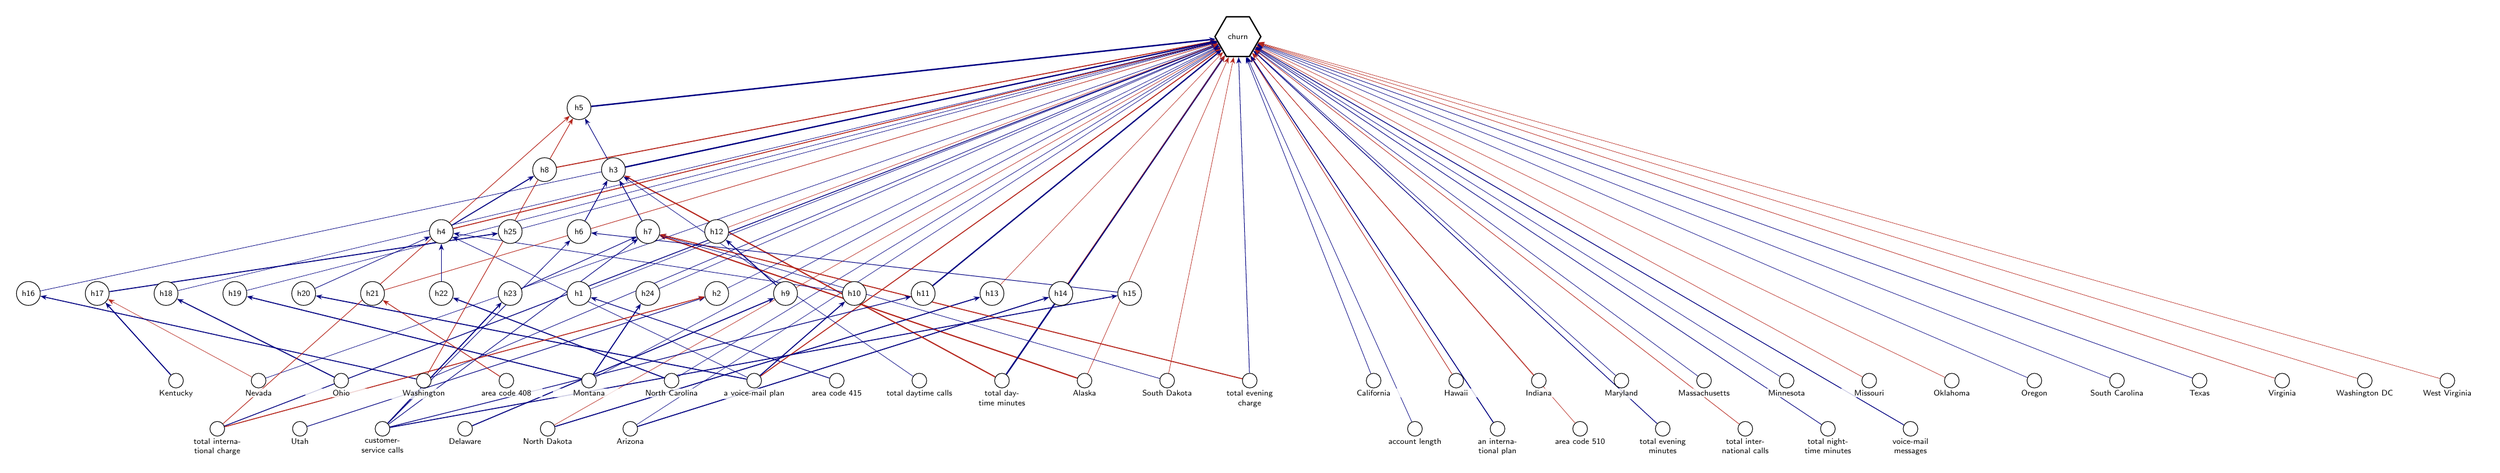
\begin{tikzpicture}[
  font=\sffamily\scriptsize, >={Stealth[length=1.4mm]},
  inp/.style={draw, circle, fill=white, minimum size=3.2mm, inner sep=0pt},
  hid/.style={draw, circle, fill=white, minimum size=5.2mm, inner sep=0.5pt, font=\sffamily\tiny},
  exitbox/.style={draw, thick, rectangle, fill=white, align=center, text width=17mm, minimum height=5mm, inner sep=1.5pt, font=\sffamily\tiny},
  sumbox/.style={draw, thick, dashed, rectangle, fill=white, align=center, text width=17mm, minimum height=5mm, inner sep=1.5pt, font=\sffamily\tiny},
  outp/.style={draw, thick, regular polygon, regular polygon sides=6, fill=white, minimum size=10mm, inner sep=0pt, font=\sffamily\tiny, align=center},
  stub/.style={draw, dashed, rounded corners=2pt, fill=white, align=center, inner sep=2pt, font=\sffamily\tiny, text width=15mm},
  inlab/.style={font=\sffamily\tiny, align=center, text width=15mm, inner sep=1pt, fill=white, fill opacity=0.8, text opacity=1},
  wpos/.style={draw=NavyBlue}, wneg/.style={draw=BrickRed}, wagg/.style={draw=black!45, line width=1.2pt},
  wmix/.style={draw=Plum},
]
\node[inp] (ninxxstatex17) at (0.0,0.0) {};
\path (ninxxstatex17.south) node[inlab, anchor=north] (labninxxstatex17) {Kentucky};
\node[inp] (ninxxstatex19) at (33.3,0.0) {};
\path (ninxxstatex19.south) node[inlab, anchor=north] (labninxxstatex19) {Massachusetts};
\node[inp] (ninxxstatex20) at (31.5,0.0) {};
\path (ninxxstatex20.south) node[inlab, anchor=north] (labninxxstatex20) {Maryland};
\node[inp] (ninxxstatex23) at (35.1,0.0) {};
\path (ninxxstatex23.south) node[inlab, anchor=north] (labninxxstatex23) {Minnesota};
\node[inp] (ninxxstatex24) at (36.9,0.0) {};
\path (ninxxstatex24.south) node[inlab, anchor=north] (labninxxstatex24) {Missouri};
\node[inp] (ninxxstatex0) at (19.8,0.0) {};
\path (ninxxstatex0.south) node[inlab, anchor=north] (labninxxstatex0) {Alaska};
\node[inp] (ninxxstatex26) at (9.0,0.0) {};
\path (ninxxstatex26.south) node[inlab, anchor=north] (labninxxstatex26) {Montana};
\node[inp] (ninxxstatex27) at (10.8,0.0) {};
\path (ninxxstatex27.south) node[inlab, anchor=north] (labninxxstatex27) {North Carolina};
\node[inp] (ninxxstatex28) at (8.1,-1.05) {};
\path (ninxxstatex28.south) node[inlab, anchor=north] (labninxxstatex28) {North Dakota};
\node[inp] (ninxxstatex3) at (9.9,-1.05) {};
\path (ninxxstatex3.south) node[inlab, anchor=north] (labninxxstatex3) {Arizona};
\node[inp] (ninxxstatex33) at (1.8,0.0) {};
\path (ninxxstatex33.south) node[inlab, anchor=north] (labninxxstatex33) {Nevada};
\node[inp] (ninxxstatex35) at (3.6,0.0) {};
\path (ninxxstatex35.south) node[inlab, anchor=north] (labninxxstatex35) {Ohio};
\node[inp] (ninxxstatex36) at (38.7,0.0) {};
\path (ninxxstatex36.south) node[inlab, anchor=north] (labninxxstatex36) {Oklahoma};
\node[inp] (ninxxstatex37) at (40.5,0.0) {};
\path (ninxxstatex37.south) node[inlab, anchor=north] (labninxxstatex37) {Oregon};
\node[inp] (ninxxstatex4) at (26.1,0.0) {};
\path (ninxxstatex4.south) node[inlab, anchor=north] (labninxxstatex4) {California};
\node[inp] (ninxxstatex40) at (42.3,0.0) {};
\path (ninxxstatex40.south) node[inlab, anchor=north] (labninxxstatex40) {South Carolina};
\node[inp] (ninxxstatex41) at (21.6,0.0) {};
\path (ninxxstatex41.south) node[inlab, anchor=north] (labninxxstatex41) {South Dakota};
\node[inp] (ninxxstatex43) at (44.1,0.0) {};
\path (ninxxstatex43.south) node[inlab, anchor=north] (labninxxstatex43) {Texas};
\node[inp] (ninxxstatex11) at (27.9,0.0) {};
\path (ninxxstatex11.south) node[inlab, anchor=north] (labninxxstatex11) {Hawaii};
\node[inp] (ninxxstatex44) at (2.7,-1.05) {};
\path (ninxxstatex44.south) node[inlab, anchor=north] (labninxxstatex44) {Utah};
\node[inp] (ninxxstatex45) at (45.9,0.0) {};
\path (ninxxstatex45.south) node[inlab, anchor=north] (labninxxstatex45) {Virginia};
\node[inp] (ninxxstatex47) at (5.4,0.0) {};
\path (ninxxstatex47.south) node[inlab, anchor=north] (labninxxstatex47) {Washington};
\node[inp] (ninxxstatex49) at (49.5,0.0) {};
\path (ninxxstatex49.south) node[inlab, anchor=north] (labninxxstatex49) {West Virginia};
\node[inp] (ninxxstatex7) at (47.7,0.0) {};
\path (ninxxstatex7.south) node[inlab, anchor=north] (labninxxstatex7) {Washington DC};
\node[inp] (ninxxstatex8) at (6.3,-1.05) {};
\path (ninxxstatex8.south) node[inlab, anchor=north] (labninxxstatex8) {Delaware};
\node[inp] (ninxxaccountxlength) at (27.0,-1.05) {};
\path (ninxxaccountxlength.south) node[inlab, anchor=north] (labninxxaccountxlength) {account length};
\node[inp] (ninxxareaxcodex408) at (7.2,0.0) {};
\path (ninxxareaxcodex408.south) node[inlab, anchor=north] (labninxxareaxcodex408) {area code 408};
\node[inp] (ninxxareaxcodex415) at (14.4,0.0) {};
\path (ninxxareaxcodex415.south) node[inlab, anchor=north] (labninxxareaxcodex415) {area code 415};
\node[inp] (ninxxareaxcodex510) at (30.6,-1.05) {};
\path (ninxxareaxcodex510.south) node[inlab, anchor=north] (labninxxareaxcodex510) {area code 510};
\node[inp] (ninxxinternationalxplan) at (28.8,-1.05) {};
\path (ninxxinternationalxplan.south) node[inlab, anchor=north] (labninxxinternationalxplan) {an international plan};
\node[inp] (ninxxvoicexmailxplan) at (12.6,0.0) {};
\path (ninxxvoicexmailxplan.south) node[inlab, anchor=north] (labninxxvoicexmailxplan) {a voice-mail plan};
\node[inp] (ninxxnumberxvmailxmessages) at (37.8,-1.05) {};
\path (ninxxnumberxvmailxmessages.south) node[inlab, anchor=north] (labninxxnumberxvmailxmessages) {voice-mail messages};
\node[inp] (ninxxtotalxdayxminutes) at (18.0,0.0) {};
\path (ninxxtotalxdayxminutes.south) node[inlab, anchor=north] (labninxxtotalxdayxminutes) {total daytime minutes};
\node[inp] (ninxxtotalxdayxcalls) at (16.2,0.0) {};
\path (ninxxtotalxdayxcalls.south) node[inlab, anchor=north] (labninxxtotalxdayxcalls) {total daytime calls};
\node[inp] (ninxxtotalxevexminutes) at (32.4,-1.05) {};
\path (ninxxtotalxevexminutes.south) node[inlab, anchor=north] (labninxxtotalxevexminutes) {total evening minutes};
\node[inp] (ninxxtotalxevexcharge) at (23.4,0.0) {};
\path (ninxxtotalxevexcharge.south) node[inlab, anchor=north] (labninxxtotalxevexcharge) {total evening charge};
\node[inp] (ninxxtotalxnightxminutes) at (36.0,-1.05) {};
\path (ninxxtotalxnightxminutes.south) node[inlab, anchor=north] (labninxxtotalxnightxminutes) {total night-time minutes};
\node[inp] (ninxxtotalxintlxcalls) at (34.2,-1.05) {};
\path (ninxxtotalxintlxcalls.south) node[inlab, anchor=north] (labninxxtotalxintlxcalls) {total international calls};
\node[inp] (ninxxtotalxintlxcharge) at (0.9,-1.05) {};
\path (ninxxtotalxintlxcharge.south) node[inlab, anchor=north] (labninxxtotalxintlxcharge) {total international charge};
\node[inp] (ninxxnumberxcustomerxservicexcalls) at (4.5,-1.05) {};
\path (ninxxnumberxcustomerxservicexcalls.south) node[inlab, anchor=north] (labninxxnumberxcustomerxservicexcalls) {customer-service calls};
\node[inp] (ninxxstatex15) at (29.7,0.0) {};
\path (ninxxstatex15.south) node[inlab, anchor=north] (labninxxstatex15) {Indiana};
\node[outp] (n0) at (23.142,7.5) {churn};
\node[hid] (n10332) at (-3.217,1.9) {h16};
\node[hid] (n11261) at (-1.717,1.9) {h17};
\node[hid] (n1133) at (5.783,3.25) {h4};
\node[hid] (n1264) at (8.783,5.95) {h5};
\node[hid] (n13551) at (-0.217,1.9) {h18};
\node[hid] (n13725) at (1.283,1.9) {h19};
\node[hid] (n13852) at (2.783,1.9) {h20};
\node[hid] (n14653) at (4.283,1.9) {h21};
\node[hid] (n14955) at (5.783,1.9) {h22};
\node[hid] (n15509) at (7.283,1.9) {h23};
\node[hid] (n161) at (8.783,1.9) {h1};
\node[hid] (n16344) at (10.283,1.9) {h24};
\node[hid] (n16902) at (7.283,3.25) {h25};
\node[hid] (n252) at (11.783,1.9) {h2};
\node[hid] (n2627) at (8.783,3.25) {h6};
\node[hid] (n2796) at (10.283,3.25) {h7};
\node[hid] (n4051) at (8.033,4.6) {h8};
\node[hid] (n4967) at (13.283,1.9) {h9};
\node[hid] (n5577) at (14.783,1.9) {h10};
\node[hid] (n7208) at (16.283,1.9) {h11};
\node[hid] (n7647) at (11.783,3.25) {h12};
\node[hid] (n807) at (9.533,4.6) {h3};
\node[hid] (n8418) at (17.783,1.9) {h13};
\node[hid] (n8896) at (19.283,1.9) {h14};
\node[hid] (n9555) at (20.783,1.9) {h15};
\begin{scope}[on background layer]
\draw[->, wneg, line width=0.27pt] (ninxxstatex0) -- (n0);
\draw[->, wneg, line width=0.74pt] (ninxxstatex0) -- (n2796);
\draw[->, wpos, line width=0.60pt] (ninxxstatex17) -- (n11261);
\draw[->, wpos, line width=0.27pt] (ninxxstatex19) -- (n0);
\draw[->, wpos, line width=0.28pt] (ninxxstatex20) -- (n0);
\draw[->, wpos, line width=0.27pt] (ninxxstatex23) -- (n0);
\draw[->, wneg, line width=0.26pt] (ninxxstatex24) -- (n0);
\draw[->, wpos, line width=0.27pt] (ninxxstatex26) -- (n0);
\draw[->, wpos, line width=0.60pt] (ninxxstatex26) -- (n13725);
\draw[->, wpos, line width=0.60pt] (ninxxstatex26) -- (n16344);
\draw[->, wpos, line width=0.26pt] (ninxxstatex27) -- (n0);
\draw[->, wpos, line width=0.60pt] (ninxxstatex27) -- (n14955);
\draw[->, wneg, line width=0.26pt] (ninxxstatex28) -- (n0);
\draw[->, wpos, line width=0.60pt] (ninxxstatex28) -- (n8418);
\draw[->, wpos, line width=0.25pt] (ninxxstatex3) -- (n0);
\draw[->, wpos, line width=0.60pt] (ninxxstatex3) -- (n8896);
\draw[->, wpos, line width=0.27pt] (ninxxstatex33) -- (n0);
\draw[->, wneg, line width=0.26pt] (ninxxstatex33) -- (n11261);
\draw[->, wpos, line width=0.60pt] (ninxxstatex35) -- (n13551);
\draw[->, wneg, line width=0.25pt] (ninxxstatex36) -- (n0);
\draw[->, wpos, line width=0.26pt] (ninxxstatex37) -- (n0);
\draw[->, wpos, line width=0.30pt] (ninxxstatex4) -- (n0);
\draw[->, wpos, line width=0.27pt] (ninxxstatex40) -- (n0);
\draw[->, wneg, line width=0.28pt] (ninxxstatex41) -- (n0);
\draw[->, wpos, line width=0.30pt] (ninxxstatex41) -- (n2796);
\draw[->, wpos, line width=0.30pt] (ninxxstatex43) -- (n0);
\draw[->, wneg, line width=0.34pt] (ninxxstatex11) -- (n0);
\draw[->, wpos, line width=0.40pt] (ninxxstatex44) -- (n252);
\draw[->, wneg, line width=0.29pt] (ninxxstatex45) -- (n0);
\draw[->, wpos, line width=0.31pt] (ninxxstatex47) -- (n0);
\draw[->, wpos, line width=0.56pt] (ninxxstatex47) -- (n10332);
\draw[->, wneg, line width=0.39pt] (ninxxstatex47) -- (n1264);
\draw[->, wneg, line width=0.25pt] (ninxxstatex49) -- (n0);
\draw[->, wneg, line width=0.26pt] (ninxxstatex7) -- (n0);
\draw[->, wpos, line width=0.59pt] (ninxxstatex8) -- (n4967);
\draw[->, wpos, line width=0.29pt] (ninxxaccountxlength) -- (n0);
\draw[->, wneg, line width=0.44pt] (ninxxareaxcodex408) -- (n14653);
\draw[->, wpos, line width=0.45pt] (ninxxareaxcodex415) -- (n161);
\draw[->, wneg, line width=0.26pt] (ninxxareaxcodex510) -- (n0);
\draw[->, wpos, line width=0.52pt] (ninxxinternationalxplan) -- (n0);
\draw[->, wneg, line width=0.56pt] (ninxxvoicexmailxplan) -- (n0);
\draw[->, wpos, line width=0.29pt] (ninxxvoicexmailxplan) -- (n1133);
\draw[->, wpos, line width=0.60pt] (ninxxvoicexmailxplan) -- (n13852);
\draw[->, wpos, line width=0.59pt] (ninxxvoicexmailxplan) -- (n5577);
\draw[->, wpos, line width=0.45pt] (ninxxnumberxvmailxmessages) -- (n0);
\draw[->, wpos, line width=0.90pt] (ninxxtotalxdayxminutes) -- (n0);
\draw[->, wneg, line width=0.71pt] (ninxxtotalxdayxminutes) -- (n807);
\draw[->, wpos, line width=0.27pt] (ninxxtotalxdayxcalls) -- (n807);
\draw[->, wpos, line width=0.42pt] (ninxxtotalxevexminutes) -- (n0);
\draw[->, wpos, line width=0.37pt] (ninxxtotalxevexcharge) -- (n0);
\draw[->, wneg, line width=0.60pt] (ninxxtotalxevexcharge) -- (n2796);
\draw[->, wpos, line width=0.35pt] (ninxxtotalxnightxminutes) -- (n0);
\draw[->, wneg, line width=0.31pt] (ninxxtotalxintlxcalls) -- (n0);
\draw[->, wpos, line width=0.49pt] (ninxxtotalxintlxcharge) -- (n0);
\draw[->, wneg, line width=0.37pt] (ninxxtotalxintlxcharge) -- (n1264);
\draw[->, wneg, line width=0.55pt] (ninxxtotalxintlxcharge) -- (n252);
\draw[->, wpos, line width=0.60pt] (ninxxnumberxcustomerxservicexcalls) -- (n15509);
\draw[->, wpos, line width=0.33pt] (ninxxnumberxcustomerxservicexcalls) -- (n2627);
\draw[->, wpos, line width=0.36pt] (ninxxnumberxcustomerxservicexcalls) -- (n2796);
\draw[->, wpos, line width=0.45pt] (ninxxnumberxcustomerxservicexcalls) -- (n7208);
\draw[->, wpos, line width=0.57pt] (ninxxnumberxcustomerxservicexcalls) -- (n9555);
\draw[->, wneg, line width=0.25pt] (ninxxstatex15) -- (n0);
\draw[->, wpos, line width=0.29pt] (n10332) -- (n0);
\draw[->, wpos, line width=0.60pt] (n11261) -- (n16902);
\draw[->, wneg, line width=0.56pt] (n1133) -- (n0);
\draw[->, wpos, line width=0.58pt] (n1133) -- (n4051);
\draw[->, wpos, line width=0.88pt] (n1264) -- (n0);
\draw[->, wpos, line width=0.27pt] (n13551) -- (n0);
\draw[->, wpos, line width=0.27pt] (n13725) -- (n0);
\draw[->, wpos, line width=0.33pt] (n13852) -- (n1133);
\draw[->, wneg, line width=0.34pt] (n14653) -- (n0);
\draw[->, wpos, line width=0.26pt] (n14955) -- (n1133);
\draw[->, wpos, line width=0.38pt] (n15509) -- (n2796);
\draw[->, wpos, line width=0.27pt] (n161) -- (n0);
\draw[->, wpos, line width=0.27pt] (n16344) -- (n0);
\draw[->, wpos, line width=0.27pt] (n16902) -- (n0);
\draw[->, wpos, line width=0.25pt] (n252) -- (n0);
\draw[->, wpos, line width=0.46pt] (n2627) -- (n807);
\draw[->, wpos, line width=0.45pt] (n2796) -- (n807);
\draw[->, wneg, line width=0.60pt] (n4051) -- (n0);
\draw[->, wpos, line width=0.59pt] (n4967) -- (n7647);
\draw[->, wpos, line width=0.32pt] (n5577) -- (n1133);
\draw[->, wpos, line width=0.78pt] (n7208) -- (n0);
\draw[->, wneg, line width=0.25pt] (n7647) -- (n0);
\draw[->, wpos, line width=0.80pt] (n807) -- (n0);
\draw[->, wpos, line width=0.37pt] (n807) -- (n1264);
\draw[->, wneg, line width=0.25pt] (n8418) -- (n0);
\draw[->, wneg, line width=0.25pt] (n8896) -- (n0);
\draw[->, wpos, line width=0.38pt] (n9555) -- (n2627);
\end{scope}
\end{tikzpicture}}%
\caption{The network as trained, before any explanation, in full. Blue: positive weight (raises the score); red: negative weight (lowers it); thicker: larger weight. Orange outline and up arrow: raises the final prediction; teal and down arrow: lowers it; grey and double arrow: depends. Not used (no connection): Alabama, Georgia, Iowa, Idaho, Illinois, Kansas, Louisiana, Arkansas, Maine, Michigan, Mississippi, Nebraska, New Hampshire, New Jersey, New Mexico, New York, Pennsylvania, Rhode Island, Tennessee, Vermont, Wisconsin, Colorado, Wyoming, Connecticut, Florida, total daytime charge, total evening calls, total night-time calls, total night-time charge, total international minutes.}
\label{fig:churn100s2c2:raw}
\end{figure}
\end{landscape}
\end{drafted}
\clearpage
\begin{drafted}[plain-language layer: churn100-s4-c2]
\section{churn100-s4-c2}
\noindent{\small Genome \texttt{4206744f-b5ce-4488-bc53-a39aa08fe972}, explanation \texttt{33d6db5d-fbdf-41c8-a597-fc997715b92f}. Split: train primary (n=4000), test as a check (n=1000). Claims: 113, verified 110, not supported 3.\par}
\noindent{\small\textcolor{BrickRed}{AI-assisted draft for review (unverified)}\par}\smallskip
\noindent{\footnotesize Reference (typical) customer: the typical customer: the median training customer for every number and the most common training category for every category (not a real customer). account length: 100; area code: area code 415; international plan: no international plan; number customer service calls: 1 calls; number vmail messages: 0 messages; state: West Virginia; total day calls: 100 calls; total day charge: 30.69 US dollars; total day minutes: 180 minutes; total eve calls: 100 calls; total eve charge: 17.12 US dollars; total eve minutes: 201 minutes; total intl calls: 4 calls; total intl charge: 2.78 US dollars; total intl minutes: 10 minutes; total night calls: 100 calls; total night charge: 9.02 US dollars; total night minutes: 200 minutes; voice mail plan: no voice-mail plan. Predicted chance that a customer leaves: 3\%.\par}
\subsection{Summary}
\noindent For a typical customer (in West Virginia, area code 415, no international or voice-mail plan, no voice-mail messages, 1 call to customer service and median usage) the model predicts a chance of leaving of about 3\%; it adds up six parts: fixed-weight inputs, service calls, heavy daytime use, state units, an evening unit and a small voice-mail unit.\,{\scriptsize\textcolor{NavyBlue}{[C046]}} Figure~\ref{fig:churn100s4c2:summary} shows the model at this level: one box per paragraph below.
\par\medskip\noindent\fbox{\begin{minipage}{0.96\linewidth}\small\textbf{How to read the diagrams.} Edge colour is the sign of that one connection: blue positive, red negative; thicker is a larger weight. The outline and arrow on an input (and on a part's output box) is its overall effect on the final prediction, read from the verified claims: orange and up arrow raises it, teal and down arrow lowers it, grey and double arrow depends (it goes both ways, or differs between levels). A negative connection into a part that itself raises the prediction means that input lowers the prediction; through a hinge the overall effect can only be read from the claims, not from the edges. Up arrow means towards churn; down arrow, away from it. A double outline marks an input (or a part's output) that acts at a fixed rate everywhere: it adds the same amount to the score per unit, so it is explained by its rate alone (see 'Linear factors'); a dashed double outline, at a fixed rate on the observed data. The normal outline is an input whose effect switches on and off somewhere. For example, a voice-mail plan has a negative connection into 'Fixed-weight inputs', a part that raises the predicted chance that a customer leaves, so a voice-mail plan lowers it.\end{minipage}}\par\medskip
\begin{figure}[H]\centering
\resizebox{!}{\ifdim\height>0.5\textheight 0.5\textheight\else\height\fi}{%
\resizebox{\ifdim\width>\linewidth\linewidth\else\width\fi}{!}{%
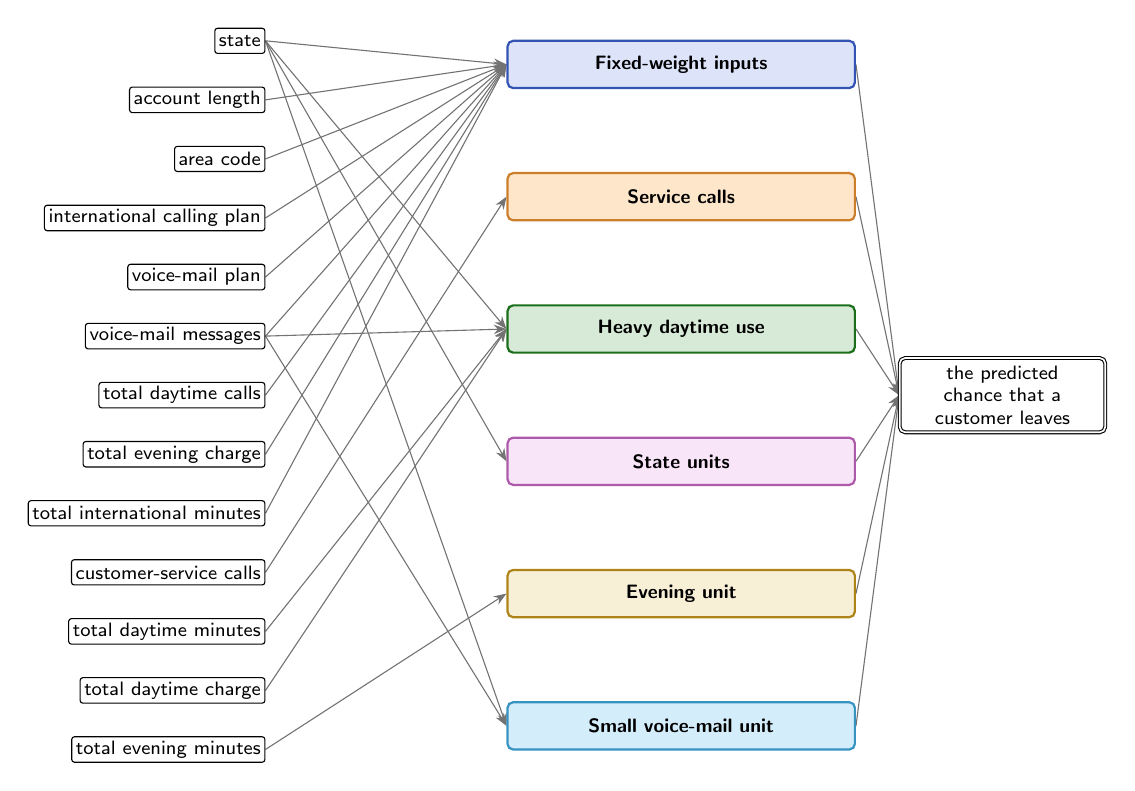
\begin{tikzpicture}[
  font=\sffamily\scriptsize, >={Stealth[length=1.6mm]},
  inp/.style={draw, rounded corners=1pt, fill=white, inner sep=1.5pt, minimum height=3.2mm, anchor=east},
  abox/.style={draw, thick, rounded corners=2pt, align=center, inner sep=3pt, minimum height=6mm, text width=42mm},
  outp/.style={draw, double, rounded corners=2pt, fill=white, align=center, inner sep=3pt, text width=24mm},
  agg/.style={draw=black!55},
]
\node[inp] (i0) at (0,4.5) {state};
\node[inp] (i1) at (0,3.75) {account length};
\node[inp] (i2) at (0,3.0) {area code};
\node[inp] (i3) at (0,2.25) {international calling plan};
\node[inp] (i4) at (0,1.5) {voice-mail plan};
\node[inp] (i5) at (0,0.75) {voice-mail messages};
\node[inp] (i6) at (0,-0.0) {total daytime calls};
\node[inp] (i7) at (0,-0.75) {total evening charge};
\node[inp] (i8) at (0,-1.5) {total international minutes};
\node[inp] (i9) at (0,-2.25) {customer-service calls};
\node[inp] (i10) at (0,-3.0) {total daytime minutes};
\node[inp] (i11) at (0,-3.75) {total daytime charge};
\node[inp] (i12) at (0,-4.5) {total evening minutes};
\node[abox, fill=RoyalBlue!18, draw=RoyalBlue!80!black] (b0) at (5.28,4.2) {\textbf{Fixed-weight inputs}};
\node[abox, fill=BurntOrange!18, draw=BurntOrange!80!black] (b1) at (5.28,2.52) {\textbf{Service calls}};
\node[abox, fill=ForestGreen!18, draw=ForestGreen!80!black] (b2) at (5.28,0.84) {\textbf{Heavy daytime use}};
\node[abox, fill=Orchid!18, draw=Orchid!80!black] (b3) at (5.28,-0.84) {\textbf{State units}};
\node[abox, fill=Goldenrod!18, draw=Goldenrod!80!black] (b4) at (5.28,-2.52) {\textbf{Evening unit}};
\node[abox, fill=Cerulean!18, draw=Cerulean!80!black] (b5) at (5.28,-4.2) {\textbf{Small voice-mail unit}};
\node[outp] (out) at (9.36,0) {the predicted chance that a customer leaves};
\begin{scope}[on background layer]
\draw[->, agg, thin] (i0.east) -- (b0.west);
\draw[->, agg, thin] (i1.east) -- (b0.west);
\draw[->, agg, thin] (i2.east) -- (b0.west);
\draw[->, agg, thin] (i3.east) -- (b0.west);
\draw[->, agg, thin] (i4.east) -- (b0.west);
\draw[->, agg, thin] (i5.east) -- (b0.west);
\draw[->, agg, thin] (i6.east) -- (b0.west);
\draw[->, agg, thin] (i7.east) -- (b0.west);
\draw[->, agg, thin] (i8.east) -- (b0.west);
\draw[->, agg] (b0.east) -- (out.west);
\draw[->, agg, thin] (i9.east) -- (b1.west);
\draw[->, agg] (b1.east) -- (out.west);
\draw[->, agg, thin] (i0.east) -- (b2.west);
\draw[->, agg, thin] (i5.east) -- (b2.west);
\draw[->, agg, thin] (i10.east) -- (b2.west);
\draw[->, agg, thin] (i11.east) -- (b2.west);
\draw[->, agg] (b2.east) -- (out.west);
\draw[->, agg, thin] (i0.east) -- (b3.west);
\draw[->, agg] (b3.east) -- (out.west);
\draw[->, agg, thin] (i12.east) -- (b4.west);
\draw[->, agg] (b4.east) -- (out.west);
\draw[->, agg, thin] (i0.east) -- (b5.west);
\draw[->, agg, thin] (i5.east) -- (b5.west);
\draw[->, agg] (b5.east) -- (out.west);
\end{scope}
\end{tikzpicture}}}%
\caption{The model at the level of the summary: one box per part.}
\label{fig:churn100s4c2:summary}
\end{figure}
\paragraph{Fixed-weight inputs.} This part adds up most inputs with fixed weights: an international plan raises a typical customer's chance of leaving from about 3\% to about 31\%, and a voice-mail plan lowers it to under 1\%.\,{\scriptsize\textcolor{NavyBlue}{[C047, C051]}} More voice-mail messages raise it steadily, from about 3\% at 0 to about 10\% at 32 messages, flattening out near the bottom because the predicted chance cannot go much lower.\,{\scriptsize\textcolor{NavyBlue}{[C049]}} A higher evening charge and more international minutes also raise it steadily, each from about 2\% to about 4\% across their usual range.\,{\scriptsize\textcolor{NavyBlue}{[C055, C056]}} Through it, the state moves the chance from about 3\% in West Virginia to about 11\% in Washington and about 7\% in New Jersey, and to under 1\% in Hawaii and in Rhode Island (72 to 122 training customers per state).\,{\scriptsize\textcolor{NavyBlue}{[C048, C050, C052, C053]}}
\paragraph{Service calls.} This part adds up two parts: a rise from 3 customer-service calls upwards and a second rise from 4 calls upwards.\,{\scriptsize\textcolor{NavyBlue}{[C079]}} From 3 calls upwards it adds to the chance slowly at first, then faster: for a typical such customer, 4 calls take it from about 3\% to about 18\%.\,{\scriptsize\textcolor{NavyBlue}{[C078]}} Up to 3 calls it barely moves a typical customer's chance, which stays at about 3\%, rising slowly at first, then faster.\,{\scriptsize\textcolor{NavyBlue}{[C077]}}
\paragraph{Heavy daytime use.} Daytime minutes add to the chance only once they rise above about 221 minutes (between 186 and 221 minutes for different customers), in an uneven way: for a typical such customer, from about 3\% at 0 minutes to about 19\% at 271 minutes.\,{\scriptsize\textcolor{NavyBlue}{[C088]}} More voice-mail messages lower it in an uneven way: for the typical customer it acts on, from about 12\% at 0 to about 6\% at 32 messages.\,{\scriptsize\textcolor{NavyBlue}{[C080]}} Customers in Washington get less from it: about 7\% instead of about 12\% for the typical customer it acts on.\,{\scriptsize\textcolor{NavyBlue}{[C082]}}
\paragraph{State units.} This part reads only the state: it raises a typical customer's chance from about 3\% to about 22\% in Rhode Island, and by less than a point in Indiana.\,{\scriptsize\textcolor{NavyBlue}{[C100, C101]}}
\paragraph{Evening unit.} This part reads evening minutes: nothing until about 217 minutes, then steadily, but a typical customer's chance stays at about 3\%.\,{\scriptsize\textcolor{NavyBlue}{[C103, C104]}}
\paragraph{Small voice-mail unit.} This small part reads voice-mail messages and being in Louisiana, and barely changes the predictions (by at most one point).\,{\scriptsize\textcolor{NavyBlue}{[C111]}}
\paragraph{The whole network.} Figure~\ref{fig:churn100s4c2:overview} (next page, landscape) draws every unit and connection of the explained model, nested by part: shaded clusters are the parts of the model and darker boxes the parts inside them; circles are hidden units (h1, h2, \ldots); each cluster's rectangle is its output, and a dashed `sum' stands for an addition the next unit does (drawn, not a unit of the model); the hexagon is the model's output. An input used by several parts is drawn under each of them (same label, dotted outline, the first copy marked with the number of copies): it is the same input, repeated for readability. Not used by the model (input columns with no connection): state: 29 of 51 levels, area code 408, area code 510, total evening calls, total night-time minutes, total night-time calls, total night-time charge, total international calls, total international charge.
\begin{landscape}
\begin{figure}[p]\centering
\resizebox{\linewidth}{!}{%
\definecolor{netup}{HTML}{D95F02}\definecolor{netdown}{HTML}{1B9E77}\definecolor{netmixed}{HTML}{7F7F7F}%
\begin{tikzpicture}[
  font=\sffamily\scriptsize, >={Stealth[length=1.4mm]},
  inp/.style={draw, circle, fill=white, minimum size=3.2mm, inner sep=0pt},
  hid/.style={draw, circle, fill=white, minimum size=5.2mm, inner sep=0.5pt, font=\sffamily\tiny},
  exitbox/.style={draw, thick, rectangle, fill=white, align=center, text width=17mm, minimum height=5mm, inner sep=1.5pt, font=\sffamily\tiny},
  sumbox/.style={draw, thick, dashed, rectangle, fill=white, align=center, text width=17mm, minimum height=5mm, inner sep=1.5pt, font=\sffamily\tiny},
  outp/.style={draw, thick, regular polygon, regular polygon sides=6, fill=white, minimum size=10mm, inner sep=0pt, font=\sffamily\tiny, align=center},
  stub/.style={draw, dashed, rounded corners=2pt, fill=white, align=center, inner sep=2pt, font=\sffamily\tiny, text width=15mm},
  inlab/.style={font=\sffamily\tiny, align=center, text width=15mm, inner sep=1pt, fill=white, fill opacity=0.8, text opacity=1},
  wpos/.style={draw=NavyBlue}, wneg/.style={draw=BrickRed}, wagg/.style={draw=black!45, line width=1.2pt},
  wmix/.style={draw=Plum},
]
\node[outp] (n0) at (22.53,7.5) {churn};
\node[hid] (n10131) at (27.59,1.9) {h9};
\node[hid] (n12171) at (18.72,3.25) {h10};
\node[hid] (n12730) at (18.72,1.9) {h11};
\node[hid] (n1295) at (33.83,1.9) {h1};
\node[hid] (n14484) at (38.42,1.9) {h12};
\node[exitbox] (n15524) at (38.42,3.25) {Evening unit $\uparrow$};
\node[hid] (n3118) at (29.09,1.9) {h2};
\node[hid] (n5268) at (18.72,4.6) {h3};
\node[exitbox] (n6089) at (43.26,1.9) {Small voice-mail unit $\uparrow$};
\node[hid] (n6713) at (14.74,3.25) {h5};
\node[hid] (n7872) at (34.58,3.25) {h6};
\node[hid] (n9436) at (14.74,1.9) {h7};
\node[hid] (n9954) at (35.33,1.9) {h8};
\node[exitbox] (nidentityxlin) at (5.85,1.9) {Fixed-weight inputs $\uparrow$};
\node[exitbox] (nidentityxsvc) at (22.2,5.95) {Service calls $\uparrow$};
\node[sumbox] (ncsumxxannx82) at (28.34,3.25) {sum: Heavy daytime use $\uparrow$};
\node[sumbox] (ncsumxxannx85) at (34.58,4.6) {sum: State units $\updownarrow$};
\node[inp, densely dotted, thick, draw=netmixed, very thick] (ngrpxxstatexxannx85) at (34.58,0.0) {};
\path (ngrpxxstatexxannx85.south) node[inlab, anchor=north] (labngrpxxstatexxannx85) {state (22 of 51 used) ($\times$4) $\updownarrow$};
\node[inp, draw=netup, very thick] (ninxxtotalxdayxminutesxxannx82) at (27.44,0.0) {};
\path (ninxxtotalxdayxminutesxxannx82.south) node[inlab, anchor=north] (labninxxtotalxdayxminutesxxannx82) {total daytime minutes $\uparrow$};
\node[inp, draw=netup, very thick] (ninxxtotalxdayxchargexxannx82) at (29.24,0.0) {};
\path (ninxxtotalxdayxchargexxannx82.south) node[inlab, anchor=north] (labninxxtotalxdayxchargexxannx82) {total daytime charge $\uparrow$};
\node[inp, draw=netup, very thick] (ninxxtotalxevexminutesxxannx83) at (38.42,0.0) {};
\path (ninxxtotalxevexminutesxxannx83.south) node[inlab, anchor=north] (labninxxtotalxevexminutesxxannx83) {total evening minutes $\uparrow$};
\node[inp, draw=netup, very thick] (ninxxnumberxcustomerxservicexcallsxxannx86) at (18.22,0.0) {};
\path (ninxxnumberxcustomerxservicexcallsxxannx86.south) node[inlab, anchor=north] (labninxxnumberxcustomerxservicexcallsxxannx86) {customer-service calls $\uparrow$};
\node[inp, densely dotted, thick, draw=netdown, very thick] (ninxxnumberxvmailxmessagesxxannx82) at (31.04,0.0) {};
\path (ninxxnumberxvmailxmessagesxxannx82.south) node[inlab, anchor=north] (labninxxnumberxvmailxmessagesxxannx82) {voice-mail messages ($\times$3) $\downarrow$};
\node[inp, densely dotted, thick, draw=netup, very thick] (ninxxnumberxvmailxmessagesxxannx84) at (44.16,0.0) {};
\path (ninxxnumberxvmailxmessagesxxannx84.south) node[inlab, anchor=north] (labninxxnumberxvmailxmessagesxxannx84) {voice-mail messages $\uparrow$};
\node[inp, densely dotted, thick, draw=netmixed, very thick] (ngrpxxstatexxannx82) at (25.64,0.0) {};
\path (ngrpxxstatexxannx82.south) node[inlab, anchor=north] (labngrpxxstatexxannx82) {state (22 of 51 used) $\updownarrow$};
\node[inp, densely dotted, thick, draw=netmixed, very thick] (ngrpxxstatexxannx84) at (42.36,0.0) {};
\path (ngrpxxstatexxannx84.south) node[inlab, anchor=north] (labngrpxxstatexxannx84) {state (22 of 51 used) $\updownarrow$};
\node[inp, densely dotted, thick, draw=netmixed, very thick] (ngrpxxstatexxannx79) at (4.5,0.0) {};
\path (ngrpxxstatexxannx79.south) node[inlab, anchor=north] (labngrpxxstatexxannx79) {state (22 of 51 used) $\updownarrow$};
\node[inp, draw=netup, very thick] (ninxxaccountxlengthxxannx79) at (1.8,-1.05) {};
\path (ninxxaccountxlengthxxannx79.south) node[inlab, anchor=north] (labninxxaccountxlengthxxannx79) {account length $\uparrow$};
\node[inp, draw=netup, very thick] (ninxxareaxcodex415xxannx79) at (3.6,-1.05) {};
\path (ninxxareaxcodex415xxannx79.south) node[inlab, anchor=north] (labninxxareaxcodex415xxannx79) {area code 415 $\uparrow$};
\node[inp, draw=netup, very thick] (ninxxinternationalxplanxxannx79) at (2.7,0.0) {};
\path (ninxxinternationalxplanxxannx79.south) node[inlab, anchor=north] (labninxxinternationalxplanxxannx79) {an international plan $\uparrow$};
\node[inp, draw=netdown, very thick] (ninxxvoicexmailxplanxxannx79) at (0.9,0.0) {};
\path (ninxxvoicexmailxplanxxannx79.south) node[inlab, anchor=north] (labninxxvoicexmailxplanxxannx79) {a voice-mail plan $\downarrow$};
\node[inp, draw=netup, very thick] (ninxxtotalxdayxcallsxxannx79) at (5.4,-1.05) {};
\path (ninxxtotalxdayxcallsxxannx79.south) node[inlab, anchor=north] (labninxxtotalxdayxcallsxxannx79) {total daytime calls $\uparrow$};
\node[inp, draw=netup, very thick] (ninxxtotalxevexchargexxannx79) at (6.3,0.0) {};
\path (ninxxtotalxevexchargexxannx79.south) node[inlab, anchor=north] (labninxxtotalxevexchargexxannx79) {total evening charge $\uparrow$};
\node[inp, draw=netup, very thick] (ninxxtotalxintlxminutesxxannx79) at (8.1,0.0) {};
\path (ninxxtotalxintlxminutesxxannx79.south) node[inlab, anchor=north] (labninxxtotalxintlxminutesxxannx79) {total international minutes $\uparrow$};
\node[inp, densely dotted, thick, draw=netup, very thick] (ninxxnumberxvmailxmessagesxxannx79) at (9.9,0.0) {};
\path (ninxxnumberxvmailxmessagesxxannx79.south) node[inlab, anchor=north] (labninxxnumberxvmailxmessagesxxannx79) {voice-mail messages $\uparrow$};
\node[font=\sffamily\tiny\bfseries, text=ForestGreen!60!black, inner sep=1pt] (subt0) at (14.74,3.75) {Calls from 4 upwards};
\node[font=\sffamily\tiny\bfseries, text=ForestGreen!60!black, inner sep=1pt] (subt1) at (18.72,5.1) {Calls from 3 upwards};
\begin{scope}[on background layer]
\node[fit=(nidentityxlin) , inner sep=8pt, rounded corners=5pt, fill=BurntOrange!10, draw=BurntOrange!45] (clu1) {};
\node[fit=(n12171) (n12730) (n5268) (n6713) (n9436) (nidentityxsvc) (subt0) (subt1), inner sep=8pt, rounded corners=5pt, fill=ForestGreen!10, draw=ForestGreen!45] (clu2) {};
\node[fit=(n10131) (n3118) (ncsumxxannx82) , inner sep=8pt, rounded corners=5pt, fill=Orchid!10, draw=Orchid!45] (clu3) {};
\node[fit=(n1295) (n7872) (n9954) (ncsumxxannx85) , inner sep=8pt, rounded corners=5pt, fill=Goldenrod!10, draw=Goldenrod!45] (clu4) {};
\node[fit=(n14484) (n15524) , inner sep=8pt, rounded corners=5pt, fill=Cerulean!10, draw=Cerulean!45] (clu5) {};
\node[fit=(n6089) , inner sep=8pt, rounded corners=5pt, fill=Mahogany!10, draw=Mahogany!45] (clu6) {};
\node[fit=(n6713) (n9436) (subt0), inner sep=4pt, rounded corners=3pt, fill=ForestGreen!26, draw=ForestGreen!70] {};
\node[fit=(n12171) (n12730) (n5268) (subt1), inner sep=4pt, rounded corners=3pt, fill=ForestGreen!26, draw=ForestGreen!70] {};
\draw[->, wneg, line width=0.60pt] (n1295) -- (ncsumxxannx85);
\draw[->, wpos, line width=0.79pt] (n3118) -- (ncsumxxannx82);
\draw[->, wpos, line width=0.25pt] (n6089) -- (n0);
\draw[->, wneg, line width=0.67pt] (n7872) -- (ncsumxxannx85);
\draw[->, wpos, line width=0.26pt] (n9954) -- (ncsumxxannx85);
\draw[->, wpos, line width=0.92pt] (n10131) -- (ncsumxxannx82);
\draw[->, wpos, line width=0.32pt] (n15524) -- (n0);
\draw[->, wpos, line width=0.44pt] (ninxxtotalxdayxminutesxxannx82) -- (n3118);
\draw[->, wpos, line width=0.38pt] (ninxxtotalxdayxchargexxannx82) -- (n3118);
\draw[->, wpos, line width=0.54pt] (ninxxtotalxdayxminutesxxannx82) -- (n10131);
\draw[->, wpos, line width=0.60pt] (ninxxtotalxevexminutesxxannx83) -- (n14484);
\draw[->, wpos, line width=0.61pt] (n1295) -- (n7872);
\draw[->, wpos, line width=0.75pt] (n9436) -- (n6713);
\draw[->, wpos, line width=0.38pt] (n12171) -- (n5268);
\draw[->, wpos, line width=0.50pt] (n12730) -- (n12171);
\draw[->, wpos, line width=0.61pt] (n14484) -- (n15524);
\draw[->, wpos, line width=0.41pt] (ninxxnumberxcustomerxservicexcallsxxannx86) -- (n9436);
\draw[->, wneg, line width=0.48pt] (ninxxnumberxvmailxmessagesxxannx82) -- (n3118);
\draw[->, wpos, line width=0.54pt] (ninxxnumberxvmailxmessagesxxannx84) -- (n6089);
\draw[->, wpos, line width=0.34pt] (ninxxnumberxcustomerxservicexcallsxxannx86) -- (n5268);
\draw[->, wpos, line width=0.55pt] (ninxxnumberxcustomerxservicexcallsxxannx86) -- (n12171);
\draw[->, wpos, line width=0.53pt] (ninxxnumberxcustomerxservicexcallsxxannx86) -- (n12730);
\draw[->, wpos, line width=0.29pt] (ninxxaccountxlengthxxannx79) -- (nidentityxlin);
\draw[->, wpos, line width=0.25pt] (ninxxareaxcodex415xxannx79) -- (nidentityxlin);
\draw[->, wpos, line width=0.54pt] (ninxxinternationalxplanxxannx79) -- (nidentityxlin);
\draw[->, wneg, line width=0.64pt] (ninxxvoicexmailxplanxxannx79) -- (nidentityxlin);
\draw[->, wpos, line width=0.30pt] (ninxxtotalxdayxcallsxxannx79) -- (nidentityxlin);
\draw[->, wpos, line width=0.37pt] (ninxxtotalxevexchargexxannx79) -- (nidentityxlin);
\draw[->, wpos, line width=0.37pt] (ninxxtotalxintlxminutesxxannx79) -- (nidentityxlin);
\draw[->, wpos, line width=0.47pt] (ninxxnumberxvmailxmessagesxxannx79) -- (nidentityxlin);
\draw[->, wpos, line width=0.60pt] (nidentityxlin) -- (n0);
\draw[->, wpos, line width=0.83pt] (n5268) -- (nidentityxsvc);
\draw[->, wpos, line width=0.87pt] (n9436) -- (nidentityxsvc);
\draw[->, wpos, line width=0.79pt] (n6713) -- (nidentityxsvc);
\draw[->, wpos, line width=0.60pt] (nidentityxsvc) -- (n0);
\draw[->, wagg] (ncsumxxannx82) -- (n0);
\draw[->, wagg] (ncsumxxannx85) -- (n0);
\draw[->, wpos, line width=0.60pt] (ngrpxxstatexxannx85) -- node[pos=0.8, sloped, above, font=\sffamily\tiny, inner sep=1pt, fill=white, fill opacity=0.8, text opacity=1] {+1.01} (n9954);
\draw[->, wneg, line width=0.49pt] (ngrpxxstatexxannx82) -- node[pos=0.8, sloped, above, font=\sffamily\tiny, inner sep=1pt, fill=white, fill opacity=0.8, text opacity=1] {-0.67} (n10131);
\draw[->, wneg, line width=0.69pt] (ngrpxxstatexxannx85) -- node[pos=0.8, sloped, above, font=\sffamily\tiny, inner sep=1pt, fill=white, fill opacity=0.8, text opacity=1] {-1.27} (n1295);
\draw[->, wpos, line width=0.65pt] (ngrpxxstatexxannx84) -- node[pos=0.8, sloped, above, font=\sffamily\tiny, inner sep=1pt, fill=white, fill opacity=0.8, text opacity=1] {+1.14} (n6089);
\draw[->, wmix, line width=0.38pt] (ngrpxxstatexxannx79) -- node[pos=0.8, sloped, above, font=\sffamily\tiny, inner sep=1pt, fill=white, fill opacity=0.8, text opacity=1] {21 edges, -0.37 to +0.16} (nidentityxlin);
\end{scope}
\node[font=\sffamily\scriptsize\bfseries, text=BurntOrange!55!black, anchor=south west, inner sep=1pt, fill=white, fill opacity=0.85, text opacity=1] at (clu1.north west) {Fixed-weight inputs};
\node[font=\sffamily\scriptsize\bfseries, text=ForestGreen!55!black, anchor=south west, inner sep=1pt, fill=white, fill opacity=0.85, text opacity=1] at (clu2.north west) {Service calls};
\node[font=\sffamily\scriptsize\bfseries, text=Orchid!55!black, anchor=south west, inner sep=1pt, fill=white, fill opacity=0.85, text opacity=1] at (clu3.north west) {Heavy daytime use};
\node[font=\sffamily\scriptsize\bfseries, text=Goldenrod!55!black, anchor=south west, inner sep=1pt, fill=white, fill opacity=0.85, text opacity=1] at (clu4.north west) {State units};
\node[font=\sffamily\scriptsize\bfseries, text=Cerulean!55!black, anchor=south west, inner sep=1pt, fill=white, fill opacity=0.85, text opacity=1] at (clu5.north west) {Evening unit};
\node[font=\sffamily\scriptsize\bfseries, text=Mahogany!55!black, anchor=south west, inner sep=1pt, fill=white, fill opacity=0.85, text opacity=1] at (clu6.north west) {Small voice-mail unit};
\end{tikzpicture}}%
\caption{Every unit and connection of the explained model, nested by part. Blue: positive weight (raises the score); red: negative weight (lowers it); thicker: larger weight. Orange outline and up arrow: raises the final prediction; teal and down arrow: lowers it; grey and double arrow: depends.}
\label{fig:churn100s4c2:overview}
\end{figure}
\end{landscape}
\paragraph{Worth checking against what is known.} Worth checking: for customers in Rhode Island the fixed-weight inputs lower the chance to under 1\% while the state units raise it to about 22\%, so overall it stays at about 3\%.\,{\scriptsize\textcolor{NavyBlue}{[C053, C100, C033]}} Worth checking: the state moves the chance by several points (Washington about 11\%, New Jersey about 7\%, Hawaii under 1\%), based on 72 to 122 training customers per state.\,{\scriptsize\textcolor{NavyBlue}{[C002, C005, C007]}} Worth checking: the model treats a voice-mail plan as lowering the chance of leaving but more voice-mail messages as raising it.\,{\scriptsize\textcolor{NavyBlue}{[C006, C003]}} Worth checking: voice-mail messages raise the chance through the fixed-weight inputs but lower it through heavy daytime use.\,{\scriptsize\textcolor{NavyBlue}{[C049, C080]}}
\subsection{The model, read from the top down}
\noindent{\small Each part of the explanation in turn, from the whole model down to the smallest parts: what it does for the prediction (hypothesis), what was checked (evidence), a diagram one level down, and where to read on. The technical record of each part is in ``Technical detail'' at the end.\par}
\subsubsection{The whole model}\label{rd:ann87}
\noindent{\small Figure~\ref{fig:churn100s4c2:parts-ann87} shows what feeds this part; Figure~\ref{fig:churn100s4c2:units-ann87} its units and every connection into them (dashed boxes: connections from or to other parts, drawn in their own sections).\par}
\begin{figure}[H]\centering
\resizebox{!}{\ifdim\height>0.5\textheight 0.5\textheight\else\height\fi}{%
\resizebox{\ifdim\width>\linewidth\linewidth\else\width\fi}{!}{%
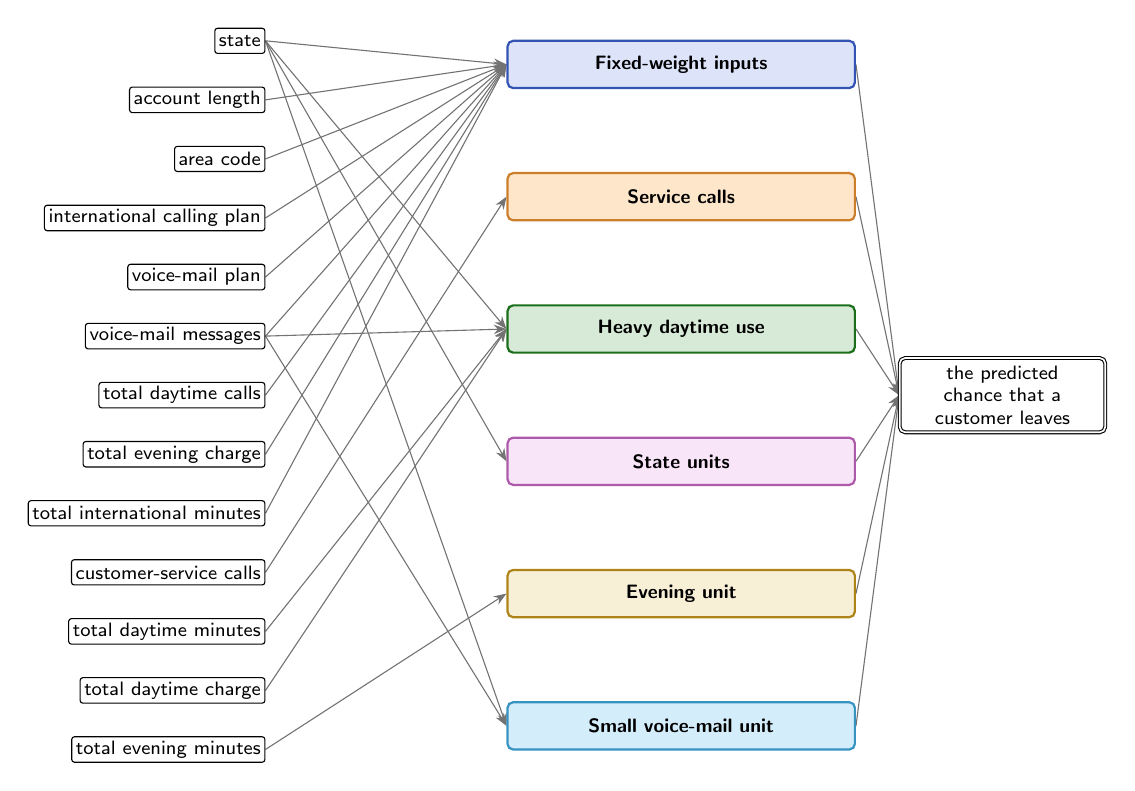
\begin{tikzpicture}[
  font=\sffamily\scriptsize, >={Stealth[length=1.6mm]},
  inp/.style={draw, rounded corners=1pt, fill=white, inner sep=1.5pt, minimum height=3.2mm, anchor=east},
  abox/.style={draw, thick, rounded corners=2pt, align=center, inner sep=3pt, minimum height=6mm, text width=42mm},
  outp/.style={draw, double, rounded corners=2pt, fill=white, align=center, inner sep=3pt, text width=24mm},
  agg/.style={draw=black!55},
]
\node[inp] (i0) at (0,4.5) {state};
\node[inp] (i1) at (0,3.75) {account length};
\node[inp] (i2) at (0,3.0) {area code};
\node[inp] (i3) at (0,2.25) {international calling plan};
\node[inp] (i4) at (0,1.5) {voice-mail plan};
\node[inp] (i5) at (0,0.75) {voice-mail messages};
\node[inp] (i6) at (0,-0.0) {total daytime calls};
\node[inp] (i7) at (0,-0.75) {total evening charge};
\node[inp] (i8) at (0,-1.5) {total international minutes};
\node[inp] (i9) at (0,-2.25) {customer-service calls};
\node[inp] (i10) at (0,-3.0) {total daytime minutes};
\node[inp] (i11) at (0,-3.75) {total daytime charge};
\node[inp] (i12) at (0,-4.5) {total evening minutes};
\node[abox, fill=RoyalBlue!18, draw=RoyalBlue!80!black] (b0) at (5.28,4.2) {\textbf{Fixed-weight inputs}};
\node[abox, fill=BurntOrange!18, draw=BurntOrange!80!black] (b1) at (5.28,2.52) {\textbf{Service calls}};
\node[abox, fill=ForestGreen!18, draw=ForestGreen!80!black] (b2) at (5.28,0.84) {\textbf{Heavy daytime use}};
\node[abox, fill=Orchid!18, draw=Orchid!80!black] (b3) at (5.28,-0.84) {\textbf{State units}};
\node[abox, fill=Goldenrod!18, draw=Goldenrod!80!black] (b4) at (5.28,-2.52) {\textbf{Evening unit}};
\node[abox, fill=Cerulean!18, draw=Cerulean!80!black] (b5) at (5.28,-4.2) {\textbf{Small voice-mail unit}};
\node[outp] (out) at (9.36,0) {the predicted chance that a customer leaves};
\begin{scope}[on background layer]
\draw[->, agg, thin] (i0.east) -- (b0.west);
\draw[->, agg, thin] (i1.east) -- (b0.west);
\draw[->, agg, thin] (i2.east) -- (b0.west);
\draw[->, agg, thin] (i3.east) -- (b0.west);
\draw[->, agg, thin] (i4.east) -- (b0.west);
\draw[->, agg, thin] (i5.east) -- (b0.west);
\draw[->, agg, thin] (i6.east) -- (b0.west);
\draw[->, agg, thin] (i7.east) -- (b0.west);
\draw[->, agg, thin] (i8.east) -- (b0.west);
\draw[->, agg] (b0.east) -- (out.west);
\draw[->, agg, thin] (i9.east) -- (b1.west);
\draw[->, agg] (b1.east) -- (out.west);
\draw[->, agg, thin] (i0.east) -- (b2.west);
\draw[->, agg, thin] (i5.east) -- (b2.west);
\draw[->, agg, thin] (i10.east) -- (b2.west);
\draw[->, agg, thin] (i11.east) -- (b2.west);
\draw[->, agg] (b2.east) -- (out.west);
\draw[->, agg, thin] (i0.east) -- (b3.west);
\draw[->, agg] (b3.east) -- (out.west);
\draw[->, agg, thin] (i12.east) -- (b4.west);
\draw[->, agg] (b4.east) -- (out.west);
\draw[->, agg, thin] (i0.east) -- (b5.west);
\draw[->, agg, thin] (i5.east) -- (b5.west);
\draw[->, agg] (b5.east) -- (out.west);
\end{scope}
\end{tikzpicture}}}%
\caption{The whole model: what feeds it, one level down.}
\label{fig:churn100s4c2:parts-ann87}
\end{figure}
\begin{figure}[H]\centering
\resizebox{\ifdim\width>\linewidth\linewidth\else\width\fi}{!}{%
\definecolor{netup}{HTML}{D95F02}\definecolor{netdown}{HTML}{1B9E77}\definecolor{netmixed}{HTML}{7F7F7F}%
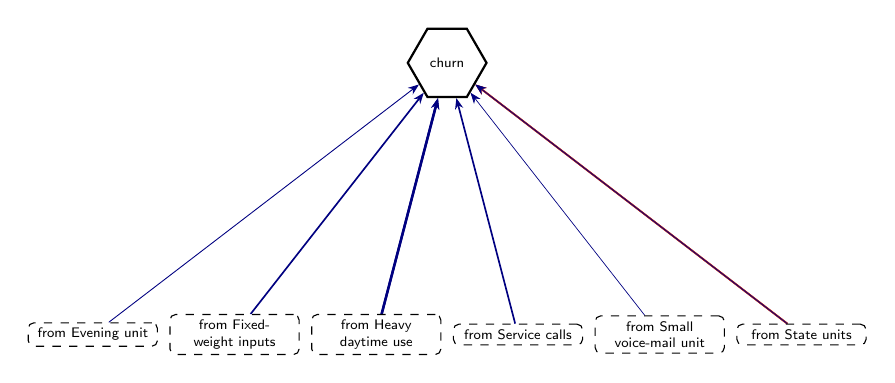
\begin{tikzpicture}[
  font=\sffamily\scriptsize, >={Stealth[length=1.4mm]},
  inp/.style={draw, circle, fill=white, minimum size=3.2mm, inner sep=0pt},
  hid/.style={draw, circle, fill=white, minimum size=5.2mm, inner sep=0.5pt, font=\sffamily\tiny},
  exitbox/.style={draw, thick, rectangle, fill=white, align=center, text width=17mm, minimum height=5mm, inner sep=1.5pt, font=\sffamily\tiny},
  sumbox/.style={draw, thick, dashed, rectangle, fill=white, align=center, text width=17mm, minimum height=5mm, inner sep=1.5pt, font=\sffamily\tiny},
  outp/.style={draw, thick, regular polygon, regular polygon sides=6, fill=white, minimum size=10mm, inner sep=0pt, font=\sffamily\tiny, align=center},
  stub/.style={draw, dashed, rounded corners=2pt, fill=white, align=center, inner sep=2pt, font=\sffamily\tiny, text width=15mm},
  inlab/.style={font=\sffamily\tiny, align=center, text width=15mm, inner sep=1pt, fill=white, fill opacity=0.8, text opacity=1},
  wpos/.style={draw=NavyBlue}, wneg/.style={draw=BrickRed}, wagg/.style={draw=black!45, line width=1.2pt},
  wmix/.style={draw=Plum},
]
\node[outp] (n0) at (5.4,3.45) {churn};
\node[stub] (nfromxxStatexunits) at (9.9,0.0) {from State units};
\node[stub] (nfromxxHeavyxdaytimexuse) at (4.5,0.0) {from Heavy daytime use};
\node[stub] (nfromxxSmallxvoicemmailxunit) at (8.1,0.0) {from Small voice-mail unit};
\node[stub] (nfromxxEveningxunit) at (0.9,0.0) {from Evening unit};
\node[stub] (nfromxxFixedmweightxinputs) at (2.7,0.0) {from Fixed-weight inputs};
\node[stub] (nfromxxServicexcalls) at (6.3,0.0) {from Service calls};
\begin{scope}[on background layer]
\draw[->, wneg, line width=0.60pt] (nfromxxStatexunits) -- (n0);
\draw[->, wpos, line width=0.79pt] (nfromxxHeavyxdaytimexuse) -- (n0);
\draw[->, wpos, line width=0.25pt] (nfromxxSmallxvoicemmailxunit) -- (n0);
\draw[->, wneg, line width=0.67pt] (nfromxxStatexunits) -- (n0);
\draw[->, wpos, line width=0.26pt] (nfromxxStatexunits) -- (n0);
\draw[->, wpos, line width=0.92pt] (nfromxxHeavyxdaytimexuse) -- (n0);
\draw[->, wpos, line width=0.32pt] (nfromxxEveningxunit) -- (n0);
\draw[->, wpos, line width=0.60pt] (nfromxxFixedmweightxinputs) -- (n0);
\draw[->, wpos, line width=0.60pt] (nfromxxServicexcalls) -- (n0);
\end{scope}
\end{tikzpicture}}%
\caption{The whole model: its units and every connection into them. Blue: positive weight (raises the score); red: negative weight (lowers it); thicker: larger weight. Orange outline and up arrow: raises the final prediction; teal and down arrow: lowers it; grey and double arrow: depends.}
\label{fig:churn100s4c2:units-ann87}
\end{figure}
\paragraph{Hypothesis.} The model adds up six parts into one score: fixed-weight inputs, service calls, heavy daytime use, state units, an evening unit and a small voice-mail unit.\,{\scriptsize\textcolor{NavyBlue}{[C046]}}
\paragraph{Evidence.} It is made up of these six parts (each explained below); the score is their sum, which was checked on all 4000 training customers.\,{\scriptsize\textcolor{NavyBlue}{[C046]}} Changing one input at a time across the whole model, an international plan takes a typical customer's chance of leaving from about 3\% to about 31\%, and a voice-mail plan lowers it to under 1\%.\,{\scriptsize\textcolor{NavyBlue}{[C001, C006]}} More daytime minutes raise it in an uneven way, from about 3\% at 112 minutes to about 8\% at 249 minutes, flattening out near the bottom because the predicted chance cannot go much lower.\,{\scriptsize\textcolor{NavyBlue}{[C004]}} In Washington the chance is about 11\%, against about 3\% in West Virginia.\,{\scriptsize\textcolor{NavyBlue}{[C002]}} The model ignores evening calls, international calls, the international charge, night-time calls, the night-time charge and night-time minutes.\,{\scriptsize\textcolor{NavyBlue}{[C040, C041, C042, C043, C044, C045]}}
\par\noindent{\small Evidence plots: Figure~\ref{fig:churn100s4c2:plot-ann87-0}, Figure~\ref{fig:churn100s4c2:plot-ann87-1}.\par}
\begin{figure}[H]\centering
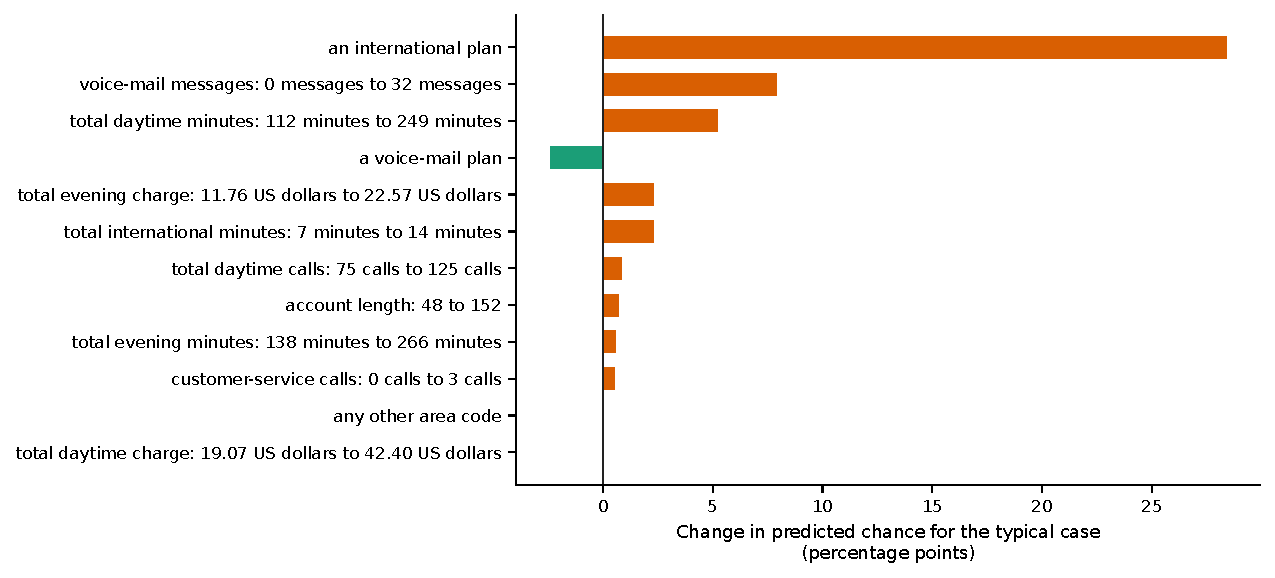
\includegraphics[width=\linewidth,height=0.88\textheight,keepaspectratio]{figures/churn100-s4-c2/ann_87-effects.pdf}
\caption{The whole model: Each input's change in the predicted value for the typical case across the whole model, largest first (orange: raises it, teal: lowers it).}
\label{fig:churn100s4c2:plot-ann87-0}
\end{figure}
\begin{figure}[H]\centering
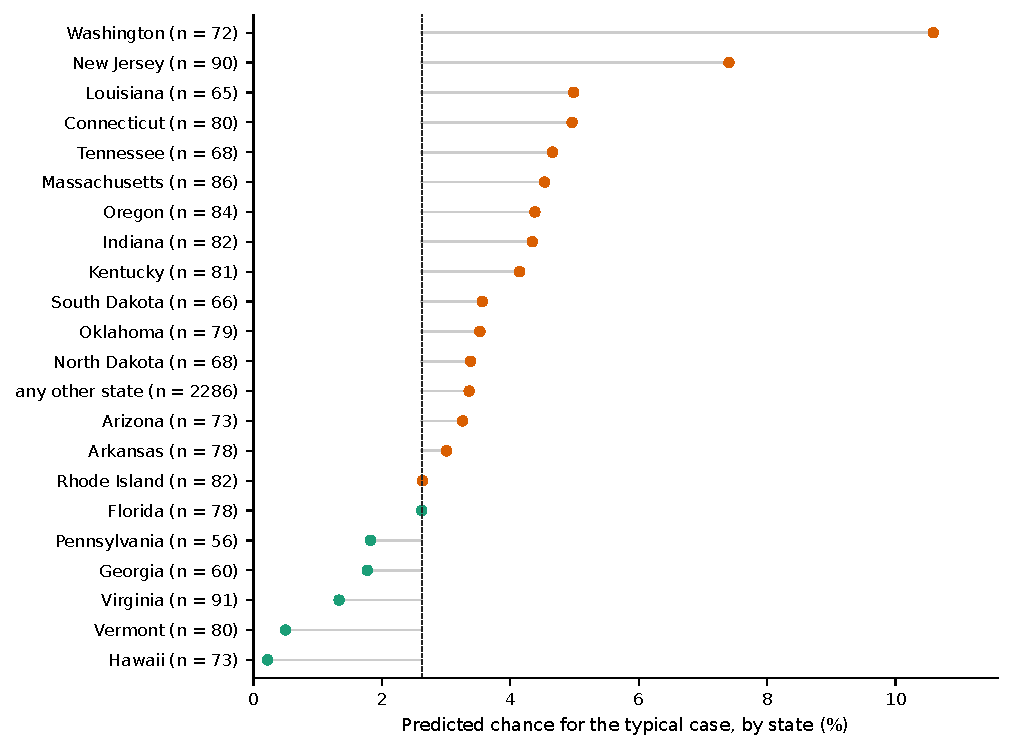
\includegraphics[width=\linewidth,height=0.88\textheight,keepaspectratio]{figures/churn100-s4-c2/ann_87-levels-state.pdf}
\caption{The whole model: Every level of state the model reads: the predicted value for the typical case at that level (dashed: the reference level); n = training customers; grey: few customers or not supported.}
\label{fig:churn100s4c2:plot-ann87-1}
\end{figure}
\par\smallskip\noindent{\small \textbf{Dive deeper:} Fixed-weight inputs (\ref{rd:ann79}); Service calls (\ref{rd:ann86}); Heavy daytime use (\ref{rd:ann82}); State units (\ref{rd:ann85}); Evening unit (\ref{rd:ann83}); Small voice-mail unit (\ref{rd:ann84}). Technical detail: \ref{tech:ann87}.\par}
\subsubsection{Fixed-weight inputs}\label{rd:ann79}
\noindent{\footnotesize Part of: The whole model (\ref{rd:ann87}).\par}
\noindent{\small Figure~\ref{fig:churn100s4c2:parts-ann79} shows what feeds this part; Figure~\ref{fig:churn100s4c2:units-ann79} its units and every connection into them (dashed boxes: connections from or to other parts, drawn in their own sections).\par}
\begin{figure}[H]\centering
\resizebox{!}{\ifdim\height>0.5\textheight 0.5\textheight\else\height\fi}{%
\resizebox{\ifdim\width>\linewidth\linewidth\else\width\fi}{!}{%
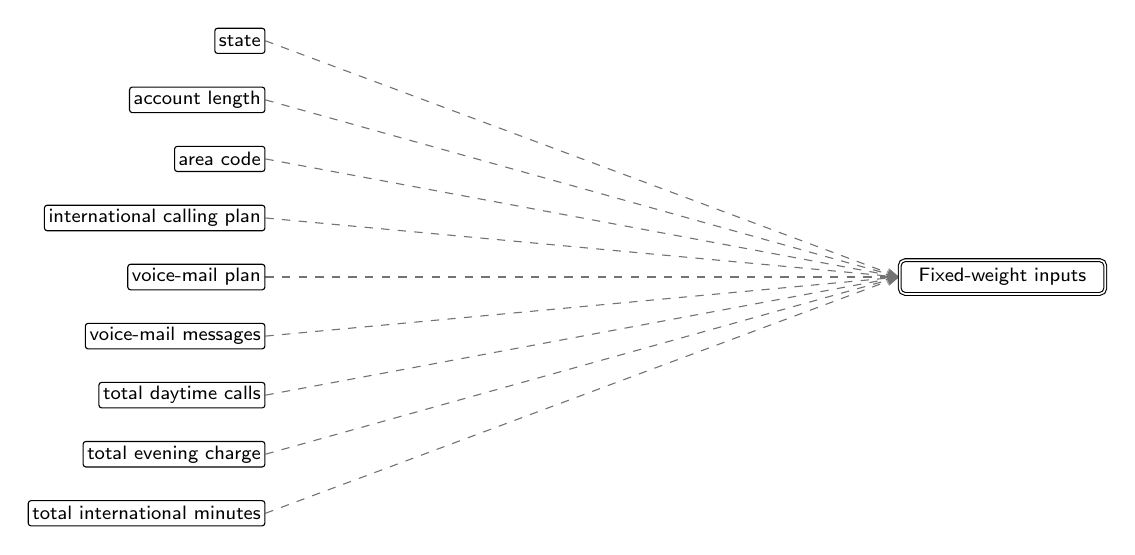
\begin{tikzpicture}[
  font=\sffamily\scriptsize, >={Stealth[length=1.6mm]},
  inp/.style={draw, rounded corners=1pt, fill=white, inner sep=1.5pt, minimum height=3.2mm, anchor=east},
  abox/.style={draw, thick, rounded corners=2pt, align=center, inner sep=3pt, minimum height=6mm, text width=42mm},
  outp/.style={draw, double, rounded corners=2pt, fill=white, align=center, inner sep=3pt, text width=24mm},
  agg/.style={draw=black!55},
]
\node[inp] (i0) at (0,3.0) {state};
\node[inp] (i1) at (0,2.25) {account length};
\node[inp] (i2) at (0,1.5) {area code};
\node[inp] (i3) at (0,0.75) {international calling plan};
\node[inp] (i4) at (0,-0.0) {voice-mail plan};
\node[inp] (i5) at (0,-0.75) {voice-mail messages};
\node[inp] (i6) at (0,-1.5) {total daytime calls};
\node[inp] (i7) at (0,-2.25) {total evening charge};
\node[inp] (i8) at (0,-3.0) {total international minutes};
\node[outp] (out) at (9.36,0) {Fixed-weight inputs};
\begin{scope}[on background layer]
\draw[->, agg, thin, dashed] (i0.east) -- (out.west);
\draw[->, agg, thin, dashed] (i1.east) -- (out.west);
\draw[->, agg, thin, dashed] (i2.east) -- (out.west);
\draw[->, agg, thin, dashed] (i3.east) -- (out.west);
\draw[->, agg, thin, dashed] (i4.east) -- (out.west);
\draw[->, agg, thin, dashed] (i5.east) -- (out.west);
\draw[->, agg, thin, dashed] (i6.east) -- (out.west);
\draw[->, agg, thin, dashed] (i7.east) -- (out.west);
\draw[->, agg, thin, dashed] (i8.east) -- (out.west);
\end{scope}
\end{tikzpicture}}}%
\caption{Fixed-weight inputs: what feeds it, one level down.}
\label{fig:churn100s4c2:parts-ann79}
\end{figure}
\begin{figure}[H]\centering
\resizebox{\ifdim\width>\linewidth\linewidth\else\width\fi}{!}{%
\definecolor{netup}{HTML}{D95F02}\definecolor{netdown}{HTML}{1B9E77}\definecolor{netmixed}{HTML}{7F7F7F}%
\begin{tikzpicture}[
  font=\sffamily\scriptsize, >={Stealth[length=1.4mm]},
  inp/.style={draw, circle, fill=white, minimum size=3.2mm, inner sep=0pt},
  hid/.style={draw, circle, fill=white, minimum size=5.2mm, inner sep=0.5pt, font=\sffamily\tiny},
  exitbox/.style={draw, thick, rectangle, fill=white, align=center, text width=17mm, minimum height=5mm, inner sep=1.5pt, font=\sffamily\tiny},
  sumbox/.style={draw, thick, dashed, rectangle, fill=white, align=center, text width=17mm, minimum height=5mm, inner sep=1.5pt, font=\sffamily\tiny},
  outp/.style={draw, thick, regular polygon, regular polygon sides=6, fill=white, minimum size=10mm, inner sep=0pt, font=\sffamily\tiny, align=center},
  stub/.style={draw, dashed, rounded corners=2pt, fill=white, align=center, inner sep=2pt, font=\sffamily\tiny, text width=15mm},
  inlab/.style={font=\sffamily\tiny, align=center, text width=15mm, inner sep=1pt, fill=white, fill opacity=0.8, text opacity=1},
  wpos/.style={draw=NavyBlue}, wneg/.style={draw=BrickRed}, wagg/.style={draw=black!45, line width=1.2pt},
  wmix/.style={draw=Plum},
]
\node[exitbox] (nidentityxlin) at (5.85,1.9) {Fixed-weight inputs $\uparrow$};
\node[inp, draw=netmixed, very thick] (ngrpxxstate) at (4.5,0.0) {};
\path (ngrpxxstate.south) node[inlab, anchor=north] (labngrpxxstate) {state (22 of 51 used) $\updownarrow$};
\node[inp, draw=netup, very thick] (ninxxaccountxlength) at (1.8,-1.05) {};
\path (ninxxaccountxlength.south) node[inlab, anchor=north] (labninxxaccountxlength) {account length $\uparrow$};
\node[inp, draw=netup, very thick] (ninxxareaxcodex415) at (3.6,-1.05) {};
\path (ninxxareaxcodex415.south) node[inlab, anchor=north] (labninxxareaxcodex415) {area code 415 $\uparrow$};
\node[inp, draw=netup, very thick] (ninxxinternationalxplan) at (2.7,0.0) {};
\path (ninxxinternationalxplan.south) node[inlab, anchor=north] (labninxxinternationalxplan) {an international plan $\uparrow$};
\node[inp, draw=netdown, very thick] (ninxxvoicexmailxplan) at (0.9,0.0) {};
\path (ninxxvoicexmailxplan.south) node[inlab, anchor=north] (labninxxvoicexmailxplan) {a voice-mail plan $\downarrow$};
\node[inp, draw=netup, very thick] (ninxxtotalxdayxcalls) at (5.4,-1.05) {};
\path (ninxxtotalxdayxcalls.south) node[inlab, anchor=north] (labninxxtotalxdayxcalls) {total daytime calls $\uparrow$};
\node[inp, draw=netup, very thick] (ninxxtotalxevexcharge) at (6.3,0.0) {};
\path (ninxxtotalxevexcharge.south) node[inlab, anchor=north] (labninxxtotalxevexcharge) {total evening charge $\uparrow$};
\node[inp, draw=netup, very thick] (ninxxtotalxintlxminutes) at (8.1,0.0) {};
\path (ninxxtotalxintlxminutes.south) node[inlab, anchor=north] (labninxxtotalxintlxminutes) {total international minutes $\uparrow$};
\node[inp, draw=netup, very thick] (ninxxnumberxvmailxmessages) at (9.9,0.0) {};
\path (ninxxnumberxvmailxmessages.south) node[inlab, anchor=north] (labninxxnumberxvmailxmessages) {voice-mail messages $\uparrow$};
\node[stub] (ntoxxthexmodelxoutput) at (5.4,3.45) {to the model output};
\begin{scope}[on background layer]
\node[fit=(nidentityxlin) , inner sep=8pt, rounded corners=5pt, fill=BurntOrange!10, draw=BurntOrange!45] (clu0) {};
\draw[->, wpos, line width=0.29pt] (ninxxaccountxlength) -- (nidentityxlin);
\draw[->, wpos, line width=0.25pt] (ninxxareaxcodex415) -- (nidentityxlin);
\draw[->, wpos, line width=0.54pt] (ninxxinternationalxplan) -- (nidentityxlin);
\draw[->, wneg, line width=0.64pt] (ninxxvoicexmailxplan) -- (nidentityxlin);
\draw[->, wpos, line width=0.30pt] (ninxxtotalxdayxcalls) -- (nidentityxlin);
\draw[->, wpos, line width=0.37pt] (ninxxtotalxevexcharge) -- (nidentityxlin);
\draw[->, wpos, line width=0.37pt] (ninxxtotalxintlxminutes) -- (nidentityxlin);
\draw[->, wpos, line width=0.47pt] (ninxxnumberxvmailxmessages) -- (nidentityxlin);
\draw[->, wpos, line width=0.60pt] (nidentityxlin) -- (ntoxxthexmodelxoutput);
\draw[->, wmix, line width=0.38pt] (ngrpxxstate) -- node[pos=0.8, sloped, above, font=\sffamily\tiny, inner sep=1pt, fill=white, fill opacity=0.8, text opacity=1] {21 edges, -0.37 to +0.16} (nidentityxlin);
\end{scope}
\node[font=\sffamily\scriptsize\bfseries, text=BurntOrange!55!black, anchor=south west, inner sep=1pt, fill=white, fill opacity=0.85, text opacity=1] at (clu0.north west) {Fixed-weight inputs};
\end{tikzpicture}}%
\caption{Fixed-weight inputs: its units and every connection into them. Blue: positive weight (raises the score); red: negative weight (lowers it); thicker: larger weight. Orange outline and up arrow: raises the final prediction; teal and down arrow: lowers it; grey and double arrow: depends.}
\label{fig:churn100s4c2:units-ann79}
\end{figure}
\paragraph{Hypothesis.} This part adds up most inputs with fixed weights: an international plan, voice-mail messages, the evening charge and international minutes raise the chance of leaving, steadily for the numbers, and a voice-mail plan lowers it.\,{\scriptsize\textcolor{NavyBlue}{[C047, C049, C055, C056, C051]}}
\paragraph{Evidence.} Through it, an international plan takes a typical customer from about 3\% to about 31\%, and a voice-mail plan lowers the chance to under 1\%.\,{\scriptsize\textcolor{NavyBlue}{[C047, C051]}} More voice-mail messages raise it steadily, from about 3\% at 0 to about 10\% at 32 messages, flattening out near the bottom because the predicted chance cannot go much lower.\,{\scriptsize\textcolor{NavyBlue}{[C049]}} Through it, the state moves the chance from about 3\% in West Virginia to about 11\% in Washington and about 7\% in New Jersey, and to under 1\% in Hawaii and in Rhode Island (72 to 122 training customers per state).\,{\scriptsize\textcolor{NavyBlue}{[C048, C050, C052, C053]}} Its formula reproduces the part exactly on all 4000 training customers.\,{\scriptsize\textcolor{NavyBlue}{[C076]}}
\par\noindent{\small Evidence plots: Figure~\ref{fig:churn100s4c2:plot-ann79-0}, Figure~\ref{fig:churn100s4c2:plot-ann79-1}, Figure~\ref{fig:churn100s4c2:plot-ann79-2}, Figure~\ref{fig:churn100s4c2:plot-ann79-3}.\par}
\begin{figure}[H]\centering
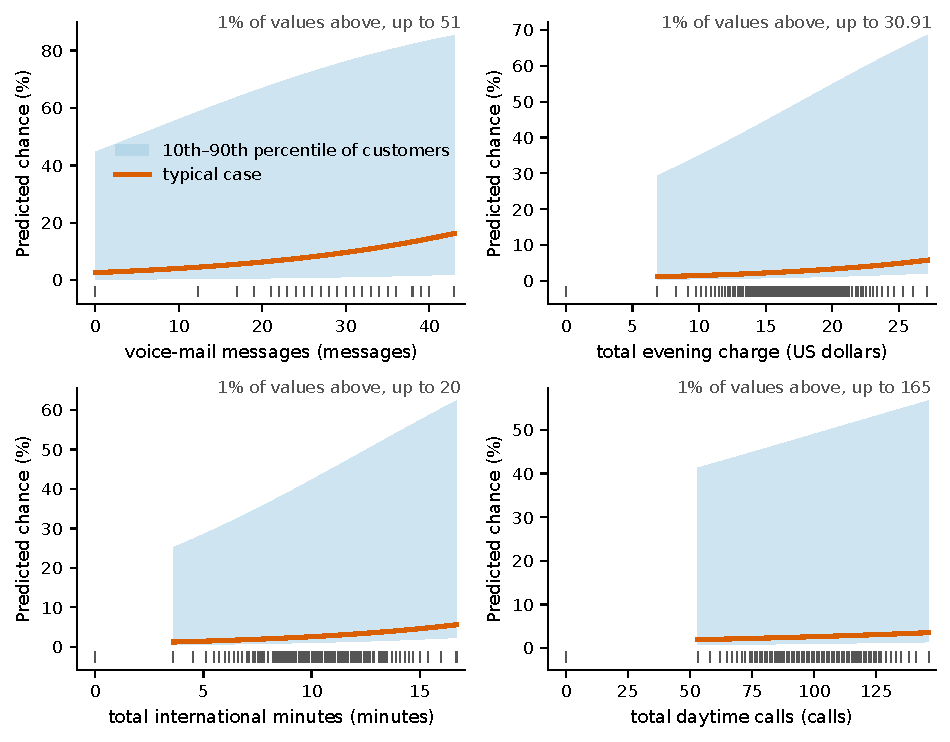
\includegraphics[width=\linewidth,height=0.88\textheight,keepaspectratio]{figures/churn100-s4-c2/ann_79-response.pdf}
\caption{Fixed-weight inputs: Response curves through this part: the typical case (bold), the 10th to 90th percentile of individual customers (band), the fold or step point (dashed) with its spread across them (grey), and the observed values (ticks).}
\label{fig:churn100s4c2:plot-ann79-0}
\end{figure}
\begin{figure}[H]\centering
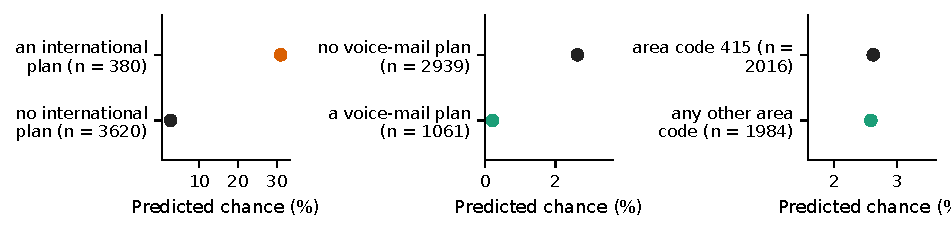
\includegraphics[width=\linewidth,height=0.88\textheight,keepaspectratio]{figures/churn100-s4-c2/ann_79-categories-small.pdf}
\caption{Fixed-weight inputs: The predicted value for the typical case at each level, through this part (n = training customers; grey: fewer than 20).}
\label{fig:churn100s4c2:plot-ann79-1}
\end{figure}
\begin{figure}[H]\centering
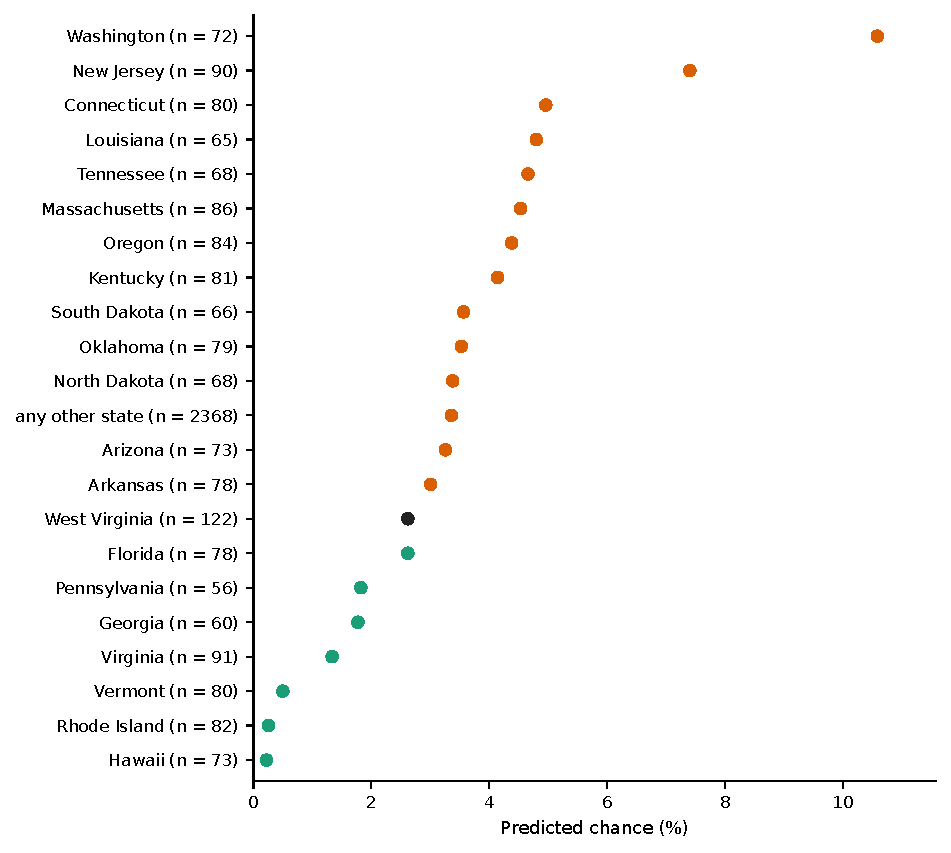
\includegraphics[width=\linewidth,height=0.88\textheight,keepaspectratio]{figures/churn100-s4-c2/ann_79-categories-C048.pdf}
\caption{Fixed-weight inputs: The predicted value for the typical case at each level, through this part (n = training customers; grey: fewer than 20).}
\label{fig:churn100s4c2:plot-ann79-2}
\end{figure}
\begin{figure}[H]\centering
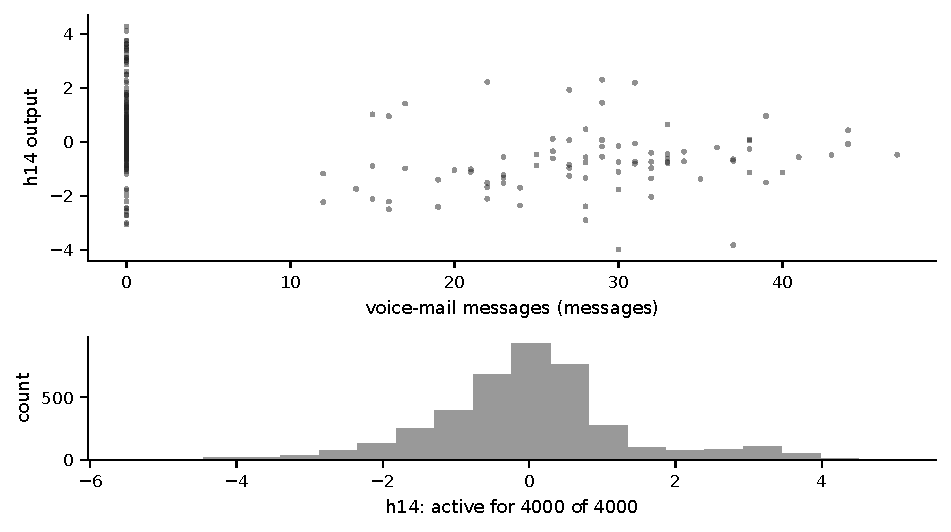
\includegraphics[width=\linewidth,height=0.88\textheight,keepaspectratio]{figures/churn100-s4-c2/ann_79-units.pdf}
\caption{Fixed-weight inputs: This part's hidden units: each unit's output against its main numeric input (top) and how often it is active (bottom).}
\label{fig:churn100s4c2:plot-ann79-3}
\end{figure}
\par\smallskip\noindent{\small Technical detail: \ref{tech:ann79}.\par}
\subsubsection{Service calls}\label{rd:ann86}
\noindent{\footnotesize Part of: The whole model (\ref{rd:ann87}).\par}
\noindent{\small Figure~\ref{fig:churn100s4c2:parts-ann86} shows what feeds this part; Figure~\ref{fig:churn100s4c2:units-ann86} its units and every connection into them (dashed boxes: connections from or to other parts, drawn in their own sections).\par}
\begin{figure}[H]\centering
\resizebox{!}{\ifdim\height>0.5\textheight 0.5\textheight\else\height\fi}{%
\resizebox{\ifdim\width>\linewidth\linewidth\else\width\fi}{!}{%
\begin{tikzpicture}[
  font=\sffamily\scriptsize, >={Stealth[length=1.6mm]},
  inp/.style={draw, rounded corners=1pt, fill=white, inner sep=1.5pt, minimum height=3.2mm, anchor=east},
  abox/.style={draw, thick, rounded corners=2pt, align=center, inner sep=3pt, minimum height=6mm, text width=42mm},
  outp/.style={draw, double, rounded corners=2pt, fill=white, align=center, inner sep=3pt, text width=24mm},
  agg/.style={draw=black!55},
]
\node[inp] (i0) at (0,-0.0) {customer-service calls};
\node[abox, fill=RoyalBlue!18, draw=RoyalBlue!80!black] (b0) at (5.28,0.5) {\textbf{Calls from 4 upwards}};
\node[abox, fill=BurntOrange!18, draw=BurntOrange!80!black] (b1) at (5.28,-0.5) {\textbf{Calls from 3 upwards}};
\node[outp] (out) at (9.36,0) {Service calls};
\begin{scope}[on background layer]
\draw[->, agg, thin] (i0.east) -- (b0.west);
\draw[->, agg] (b0.east) -- (out.west);
\draw[->, agg, thin] (i0.east) -- (b1.west);
\draw[->, agg] (b1.east) -- (out.west);
\end{scope}
\end{tikzpicture}}}%
\caption{Service calls: what feeds it, one level down.}
\label{fig:churn100s4c2:parts-ann86}
\end{figure}
\begin{figure}[H]\centering
\resizebox{\ifdim\width>\linewidth\linewidth\else\width\fi}{!}{%
\definecolor{netup}{HTML}{D95F02}\definecolor{netdown}{HTML}{1B9E77}\definecolor{netmixed}{HTML}{7F7F7F}%
\begin{tikzpicture}[
  font=\sffamily\scriptsize, >={Stealth[length=1.4mm]},
  inp/.style={draw, circle, fill=white, minimum size=3.2mm, inner sep=0pt},
  hid/.style={draw, circle, fill=white, minimum size=5.2mm, inner sep=0.5pt, font=\sffamily\tiny},
  exitbox/.style={draw, thick, rectangle, fill=white, align=center, text width=17mm, minimum height=5mm, inner sep=1.5pt, font=\sffamily\tiny},
  sumbox/.style={draw, thick, dashed, rectangle, fill=white, align=center, text width=17mm, minimum height=5mm, inner sep=1.5pt, font=\sffamily\tiny},
  outp/.style={draw, thick, regular polygon, regular polygon sides=6, fill=white, minimum size=10mm, inner sep=0pt, font=\sffamily\tiny, align=center},
  stub/.style={draw, dashed, rounded corners=2pt, fill=white, align=center, inner sep=2pt, font=\sffamily\tiny, text width=15mm},
  inlab/.style={font=\sffamily\tiny, align=center, text width=15mm, inner sep=1pt, fill=white, fill opacity=0.8, text opacity=1},
  wpos/.style={draw=NavyBlue}, wneg/.style={draw=BrickRed}, wagg/.style={draw=black!45, line width=1.2pt},
  wmix/.style={draw=Plum},
]
\node[exitbox] (nidentityxsvc) at (1.8,1.9) {Service calls $\uparrow$};
\node[stub] (nfromxxCallsxfromx3xupwards) at (0.9,0.0) {from Calls from 3 upwards};
\node[stub] (nfromxxCallsxfromx4xupwards) at (2.7,0.0) {from Calls from 4 upwards};
\node[stub] (ntoxxthexmodelxoutput) at (1.8,3.45) {to the model output};
\begin{scope}[on background layer]
\node[fit=(nidentityxsvc) , inner sep=8pt, rounded corners=5pt, fill=ForestGreen!10, draw=ForestGreen!45] (clu0) {};
\draw[->, wpos, line width=0.83pt] (nfromxxCallsxfromx3xupwards) -- (nidentityxsvc);
\draw[->, wpos, line width=0.87pt] (nfromxxCallsxfromx4xupwards) -- (nidentityxsvc);
\draw[->, wpos, line width=0.79pt] (nfromxxCallsxfromx4xupwards) -- (nidentityxsvc);
\draw[->, wpos, line width=0.60pt] (nidentityxsvc) -- (ntoxxthexmodelxoutput);
\end{scope}
\node[font=\sffamily\scriptsize\bfseries, text=ForestGreen!55!black, anchor=south west, inner sep=1pt, fill=white, fill opacity=0.85, text opacity=1] at (clu0.north west) {Service calls};
\end{tikzpicture}}%
\caption{Service calls: its units and every connection into them. Blue: positive weight (raises the score); red: negative weight (lowers it); thicker: larger weight. Orange outline and up arrow: raises the final prediction; teal and down arrow: lowers it; grey and double arrow: depends.}
\label{fig:churn100s4c2:units-ann86}
\end{figure}
\paragraph{Hypothesis.} This part raises the chance of leaving with calls to customer service from 3 calls upwards, slowly at first, then faster; it adds up two parts.\,{\scriptsize\textcolor{NavyBlue}{[C079, C078, C077]}}
\paragraph{Evidence.} It is made of two parts that are added: calls from 3 upwards and calls from 4 upwards.\,{\scriptsize\textcolor{NavyBlue}{[C079]}} From 3 calls upwards it adds to the chance slowly at first, then faster: for a typical such customer, 4 calls take it from about 3\% to about 18\%.\,{\scriptsize\textcolor{NavyBlue}{[C078]}} Up to 3 calls it barely moves a typical customer's chance, which stays at about 3\%, rising slowly at first, then faster.\,{\scriptsize\textcolor{NavyBlue}{[C077]}}
\par\noindent{\small Evidence plots: Figure~\ref{fig:churn100s4c2:plot-ann86-0}, Figure~\ref{fig:churn100s4c2:plot-ann86-1}, Figure~\ref{fig:churn100s4c2:plot-ann86-2}.\par}
\par\noindent{\small Figure~\ref{fig:churn100s4c2:plot-ann86-1} shows this part's own output, unit h15: it switches on at about 2.899 calls of customer-service calls, and is zero below.\par}
\begin{figure}[H]\centering
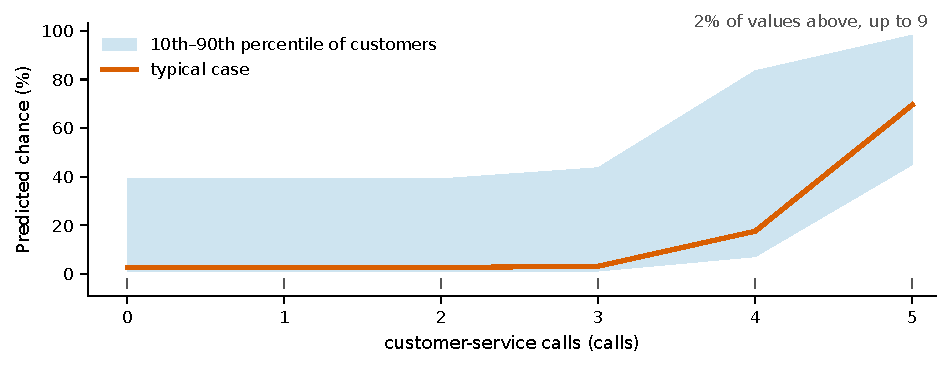
\includegraphics[width=\linewidth,height=0.88\textheight,keepaspectratio]{figures/churn100-s4-c2/ann_86-response.pdf}
\caption{Service calls: Response curves through this part: the typical case (bold), the 10th to 90th percentile of individual customers (band), the fold or step point (dashed) with its spread across them (grey), and the observed values (ticks).}
\label{fig:churn100s4c2:plot-ann86-0}
\end{figure}
\begin{figure}[H]\centering
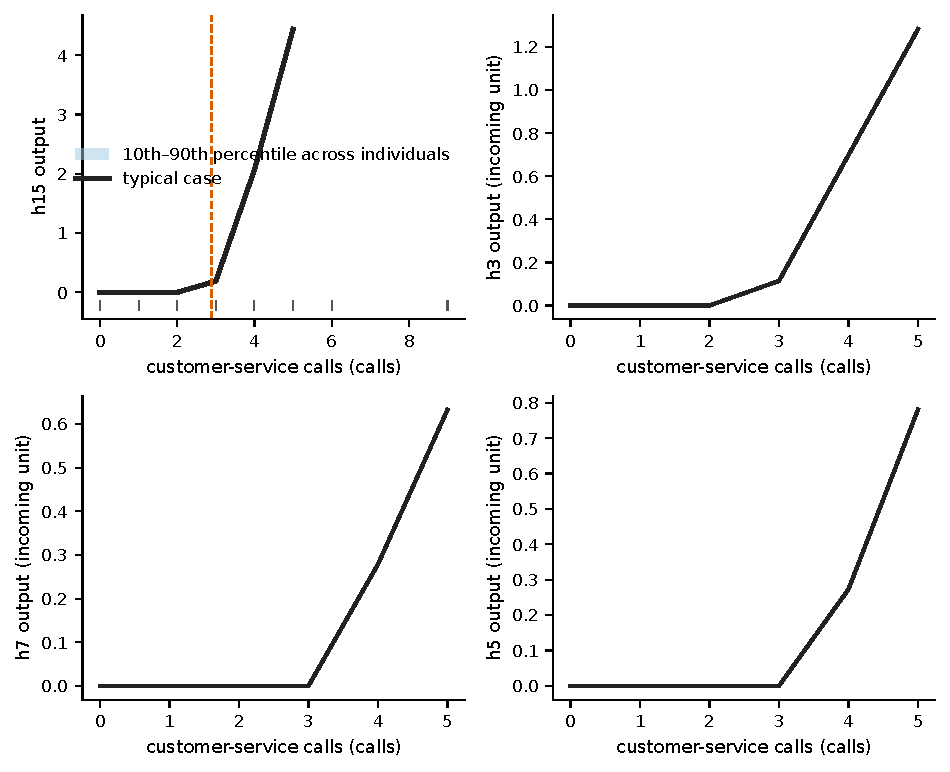
\includegraphics[width=\linewidth,height=0.88\textheight,keepaspectratio]{figures/churn100-s4-c2/ann_86-partial-identity_svc.pdf}
\caption{Service calls: This part's own output, unit h15 (combines 3 non-linear units), on its own scale (its activation), with every other input at the typical case; it is active for 848 of 4000. Bold: the typical case; band: 10th to 90th percentile across individuals; dashed: where it switches on; ticks: the data.}
\label{fig:churn100s4c2:plot-ann86-1}
\end{figure}
\begin{figure}[H]\centering
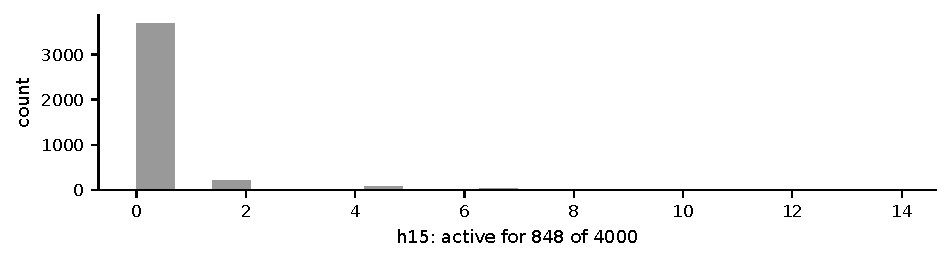
\includegraphics[width=\linewidth,height=0.88\textheight,keepaspectratio]{figures/churn100-s4-c2/ann_86-units.pdf}
\caption{Service calls: This part's hidden units: each unit's output against its main numeric input (top) and how often it is active (bottom).}
\label{fig:churn100s4c2:plot-ann86-2}
\end{figure}
\par\smallskip\noindent{\small \textbf{Dive deeper:} Calls from 4 upwards (\ref{rd:ann81}); Calls from 3 upwards (\ref{rd:ann80}). Technical detail: \ref{tech:ann86}.\par}
\subsubsection{Calls from 4 upwards}\label{rd:ann81}
\noindent{\footnotesize Part of: Service calls (\ref{rd:ann86}).\par}
\noindent{\small Figure~\ref{fig:churn100s4c2:parts-ann81} shows what feeds this part; Figure~\ref{fig:churn100s4c2:units-ann81} its units and every connection into them (dashed boxes: connections from or to other parts, drawn in their own sections).\par}
\begin{figure}[H]\centering
\resizebox{!}{\ifdim\height>0.5\textheight 0.5\textheight\else\height\fi}{%
\resizebox{\ifdim\width>\linewidth\linewidth\else\width\fi}{!}{%
\begin{tikzpicture}[
  font=\sffamily\scriptsize, >={Stealth[length=1.6mm]},
  inp/.style={draw, rounded corners=1pt, fill=white, inner sep=1.5pt, minimum height=3.2mm, anchor=east},
  abox/.style={draw, thick, rounded corners=2pt, align=center, inner sep=3pt, minimum height=6mm, text width=42mm},
  outp/.style={draw, double, rounded corners=2pt, fill=white, align=center, inner sep=3pt, text width=24mm},
  agg/.style={draw=black!55},
]
\node[inp] (i0) at (0,-0.0) {customer-service calls};
\node[outp] (out) at (9.36,0) {Calls from 4 upwards};
\begin{scope}[on background layer]
\draw[->, agg, thin, dashed] (i0.east) -- (out.west);
\end{scope}
\end{tikzpicture}}}%
\caption{Calls from 4 upwards: what feeds it, one level down.}
\label{fig:churn100s4c2:parts-ann81}
\end{figure}
\begin{figure}[H]\centering
\resizebox{\ifdim\width>\linewidth\linewidth\else\width\fi}{!}{%
\definecolor{netup}{HTML}{D95F02}\definecolor{netdown}{HTML}{1B9E77}\definecolor{netmixed}{HTML}{7F7F7F}%
\begin{tikzpicture}[
  font=\sffamily\scriptsize, >={Stealth[length=1.4mm]},
  inp/.style={draw, circle, fill=white, minimum size=3.2mm, inner sep=0pt},
  hid/.style={draw, circle, fill=white, minimum size=5.2mm, inner sep=0.5pt, font=\sffamily\tiny},
  exitbox/.style={draw, thick, rectangle, fill=white, align=center, text width=17mm, minimum height=5mm, inner sep=1.5pt, font=\sffamily\tiny},
  sumbox/.style={draw, thick, dashed, rectangle, fill=white, align=center, text width=17mm, minimum height=5mm, inner sep=1.5pt, font=\sffamily\tiny},
  outp/.style={draw, thick, regular polygon, regular polygon sides=6, fill=white, minimum size=10mm, inner sep=0pt, font=\sffamily\tiny, align=center},
  stub/.style={draw, dashed, rounded corners=2pt, fill=white, align=center, inner sep=2pt, font=\sffamily\tiny, text width=15mm},
  inlab/.style={font=\sffamily\tiny, align=center, text width=15mm, inner sep=1pt, fill=white, fill opacity=0.8, text opacity=1},
  wpos/.style={draw=NavyBlue}, wneg/.style={draw=BrickRed}, wagg/.style={draw=black!45, line width=1.2pt},
  wmix/.style={draw=Plum},
]
\node[hid] (n6713) at (2.0,3.25) {h5};
\node[hid] (n9436) at (2.0,1.9) {h7};
\node[inp, draw=netup, very thick] (ninxxnumberxcustomerxservicexcalls) at (2.0,0.0) {};
\path (ninxxnumberxcustomerxservicexcalls.south) node[inlab, anchor=north] (labninxxnumberxcustomerxservicexcalls) {customer-service calls $\uparrow$};
\node[stub] (ntoxxServicexcalls) at (2.0,4.8) {to Service calls};
\begin{scope}[on background layer]
\node[fit=(n6713) (n9436) , inner sep=8pt, rounded corners=5pt, fill=ForestGreen!10, draw=ForestGreen!45] (clu0) {};
\draw[->, wpos, line width=0.75pt] (n9436) -- (n6713);
\draw[->, wpos, line width=0.41pt] (ninxxnumberxcustomerxservicexcalls) -- (n9436);
\draw[->, wpos, line width=0.87pt] (n9436) -- (ntoxxServicexcalls);
\draw[->, wpos, line width=0.79pt] (n6713) -- (ntoxxServicexcalls);
\end{scope}
\node[font=\sffamily\scriptsize\bfseries, text=ForestGreen!55!black, anchor=south west, inner sep=1pt, fill=white, fill opacity=0.85, text opacity=1] at (clu0.north west) {Calls from 4 upwards};
\end{tikzpicture}}%
\caption{Calls from 4 upwards: its units and every connection into them. Blue: positive weight (raises the score); red: negative weight (lowers it); thicker: larger weight. Orange outline and up arrow: raises the final prediction; teal and down arrow: lowers it; grey and double arrow: depends.}
\label{fig:churn100s4c2:units-ann81}
\end{figure}
\paragraph{Hypothesis.} This part raises the chance of leaving from 4 customer-service calls upwards, slowly at first, then faster.\,{\scriptsize\textcolor{NavyBlue}{[C093]}}
\paragraph{Evidence.} It acts on 318 of 4000 training customers, 159 of whom left; for the typical customer it acts on, the chance is about 8\% without it and about 18\% with it.\,{\scriptsize\textcolor{NavyBlue}{[C094]}} Through it, the chance rises slowly at first, then faster: 4 calls take a typical such customer from about 3\% to about 6\%.\,{\scriptsize\textcolor{NavyBlue}{[C093]}} Its formula reproduces the part exactly on all 4000 training customers.\,{\scriptsize\textcolor{NavyBlue}{[C095]}}
\par\noindent{\small Evidence plots: Figure~\ref{fig:churn100s4c2:plot-ann81-0}, Figure~\ref{fig:churn100s4c2:plot-ann81-1}, Figure~\ref{fig:churn100s4c2:plot-ann81-2}.\par}
\par\noindent{\small Figure~\ref{fig:churn100s4c2:plot-ann81-0} shows this part's own output, unit h7: it switches on at about 3.212 calls of customer-service calls, and is zero below.\par}
\par\noindent{\small Figure~\ref{fig:churn100s4c2:plot-ann81-1} shows this part's own output, unit h5: it switches on at about 3.463 calls of customer-service calls, and is zero below.\par}
\begin{figure}[H]\centering
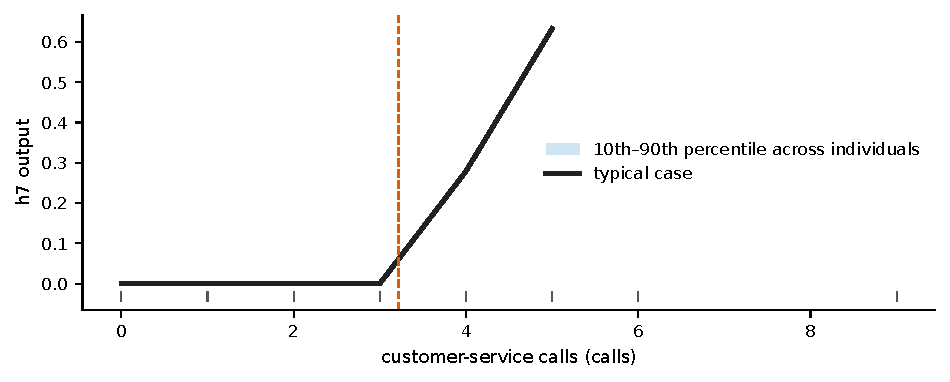
\includegraphics[width=\linewidth,height=0.88\textheight,keepaspectratio]{figures/churn100-s4-c2/ann_81-partial-9436.pdf}
\caption{Calls from 4 upwards: This part's own output, unit h7 (the output of 'Calls from 4 upwards'), on its own scale (its activation), with every other input at the typical case; it is active for 318 of 4000. Bold: the typical case; band: 10th to 90th percentile across individuals; dashed: where it switches on; ticks: the data.}
\label{fig:churn100s4c2:plot-ann81-0}
\end{figure}
\begin{figure}[H]\centering
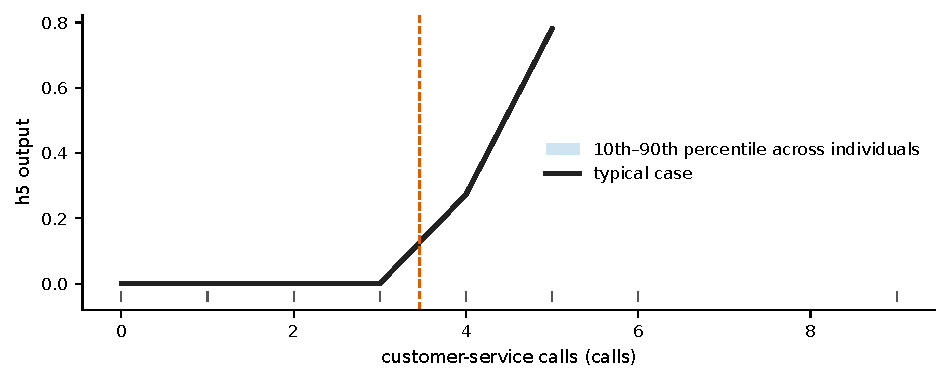
\includegraphics[width=\linewidth,height=0.88\textheight,keepaspectratio]{figures/churn100-s4-c2/ann_81-partial-6713.pdf}
\caption{Calls from 4 upwards: This part's own output, unit h5 (the output of 'Calls from 4 upwards'), on its own scale (its activation), with every other input at the typical case; it is active for 318 of 4000. Bold: the typical case; band: 10th to 90th percentile across individuals; dashed: where it switches on; ticks: the data.}
\label{fig:churn100s4c2:plot-ann81-1}
\end{figure}
\begin{figure}[H]\centering
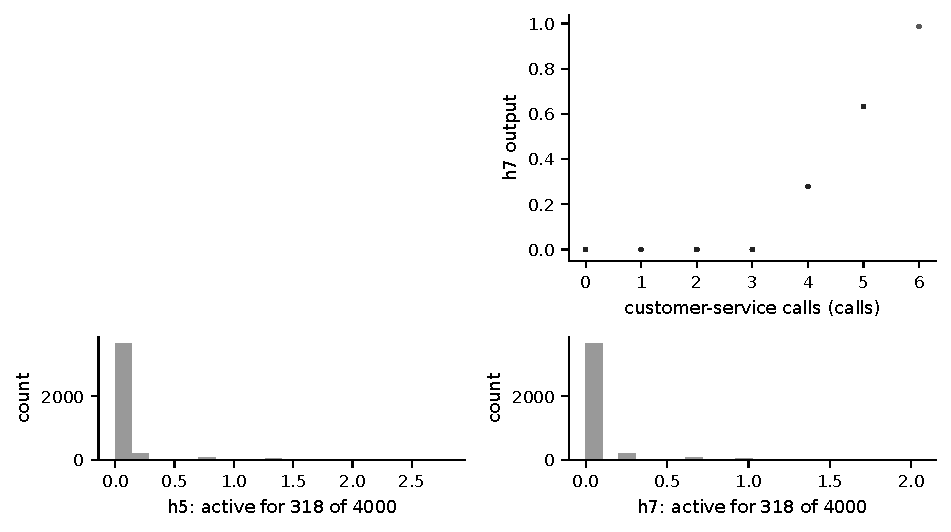
\includegraphics[width=\linewidth,height=0.88\textheight,keepaspectratio]{figures/churn100-s4-c2/ann_81-units.pdf}
\caption{Calls from 4 upwards: This part's hidden units: each unit's output against its main numeric input (top) and how often it is active (bottom).}
\label{fig:churn100s4c2:plot-ann81-2}
\end{figure}
\par\smallskip\noindent{\small Technical detail: \ref{tech:ann81}.\par}
\subsubsection{Calls from 3 upwards}\label{rd:ann80}
\noindent{\footnotesize Part of: Service calls (\ref{rd:ann86}).\par}
\noindent{\small Figure~\ref{fig:churn100s4c2:parts-ann80} shows what feeds this part; Figure~\ref{fig:churn100s4c2:units-ann80} its units and every connection into them (dashed boxes: connections from or to other parts, drawn in their own sections).\par}
\begin{figure}[H]\centering
\resizebox{!}{\ifdim\height>0.5\textheight 0.5\textheight\else\height\fi}{%
\resizebox{\ifdim\width>\linewidth\linewidth\else\width\fi}{!}{%
\begin{tikzpicture}[
  font=\sffamily\scriptsize, >={Stealth[length=1.6mm]},
  inp/.style={draw, rounded corners=1pt, fill=white, inner sep=1.5pt, minimum height=3.2mm, anchor=east},
  abox/.style={draw, thick, rounded corners=2pt, align=center, inner sep=3pt, minimum height=6mm, text width=42mm},
  outp/.style={draw, double, rounded corners=2pt, fill=white, align=center, inner sep=3pt, text width=24mm},
  agg/.style={draw=black!55},
]
\node[inp] (i0) at (0,-0.0) {customer-service calls};
\node[outp] (out) at (9.36,0) {Calls from 3 upwards};
\begin{scope}[on background layer]
\draw[->, agg, thin, dashed] (i0.east) -- (out.west);
\end{scope}
\end{tikzpicture}}}%
\caption{Calls from 3 upwards: what feeds it, one level down.}
\label{fig:churn100s4c2:parts-ann80}
\end{figure}
\begin{figure}[H]\centering
\resizebox{\ifdim\width>\linewidth\linewidth\else\width\fi}{!}{%
\definecolor{netup}{HTML}{D95F02}\definecolor{netdown}{HTML}{1B9E77}\definecolor{netmixed}{HTML}{7F7F7F}%
\begin{tikzpicture}[
  font=\sffamily\scriptsize, >={Stealth[length=1.4mm]},
  inp/.style={draw, circle, fill=white, minimum size=3.2mm, inner sep=0pt},
  hid/.style={draw, circle, fill=white, minimum size=5.2mm, inner sep=0.5pt, font=\sffamily\tiny},
  exitbox/.style={draw, thick, rectangle, fill=white, align=center, text width=17mm, minimum height=5mm, inner sep=1.5pt, font=\sffamily\tiny},
  sumbox/.style={draw, thick, dashed, rectangle, fill=white, align=center, text width=17mm, minimum height=5mm, inner sep=1.5pt, font=\sffamily\tiny},
  outp/.style={draw, thick, regular polygon, regular polygon sides=6, fill=white, minimum size=10mm, inner sep=0pt, font=\sffamily\tiny, align=center},
  stub/.style={draw, dashed, rounded corners=2pt, fill=white, align=center, inner sep=2pt, font=\sffamily\tiny, text width=15mm},
  inlab/.style={font=\sffamily\tiny, align=center, text width=15mm, inner sep=1pt, fill=white, fill opacity=0.8, text opacity=1},
  wpos/.style={draw=NavyBlue}, wneg/.style={draw=BrickRed}, wagg/.style={draw=black!45, line width=1.2pt},
  wmix/.style={draw=Plum},
]
\node[hid] (n12171) at (2.0,3.25) {h10};
\node[exitbox] (n5268) at (2.0,4.6) {Calls from 3 upwards $\uparrow$};
\node[hid] (n12730) at (2.0,1.9) {h11};
\node[inp, draw=netup, very thick] (ninxxnumberxcustomerxservicexcalls) at (2.0,0.0) {};
\path (ninxxnumberxcustomerxservicexcalls.south) node[inlab, anchor=north] (labninxxnumberxcustomerxservicexcalls) {customer-service calls $\uparrow$};
\node[stub] (ntoxxServicexcalls) at (2.0,6.15) {to Service calls};
\begin{scope}[on background layer]
\node[fit=(n12171) (n5268) (n12730) , inner sep=8pt, rounded corners=5pt, fill=ForestGreen!10, draw=ForestGreen!45] (clu0) {};
\draw[->, wpos, line width=0.38pt] (n12171) -- (n5268);
\draw[->, wpos, line width=0.50pt] (n12730) -- (n12171);
\draw[->, wpos, line width=0.34pt] (ninxxnumberxcustomerxservicexcalls) -- (n5268);
\draw[->, wpos, line width=0.55pt] (ninxxnumberxcustomerxservicexcalls) -- (n12171);
\draw[->, wpos, line width=0.53pt] (ninxxnumberxcustomerxservicexcalls) -- (n12730);
\draw[->, wpos, line width=0.83pt] (n5268) -- (ntoxxServicexcalls);
\end{scope}
\node[font=\sffamily\scriptsize\bfseries, text=ForestGreen!55!black, anchor=south west, inner sep=1pt, fill=white, fill opacity=0.85, text opacity=1] at (clu0.north west) {Calls from 3 upwards};
\end{tikzpicture}}%
\caption{Calls from 3 upwards: its units and every connection into them. Blue: positive weight (raises the score); red: negative weight (lowers it); thicker: larger weight. Orange outline and up arrow: raises the final prediction; teal and down arrow: lowers it; grey and double arrow: depends.}
\label{fig:churn100s4c2:units-ann80}
\end{figure}
\paragraph{Hypothesis.} This part raises the chance of leaving from 3 customer-service calls upwards, slowly at first, then faster.\,{\scriptsize\textcolor{NavyBlue}{[C097, C096]}}
\paragraph{Evidence.} It acts on 848 of 4000 training customers, 215 of whom left; for the typical customer it acts on, the chance is about 3\% without it and about 4\% with it.\,{\scriptsize\textcolor{NavyBlue}{[C098]}} Through it, the chance rises slowly at first, then faster: 4 calls take a typical such customer from about 3\% to about 8\%.\,{\scriptsize\textcolor{NavyBlue}{[C097]}} Its formula reproduces the part exactly on all 4000 training customers.\,{\scriptsize\textcolor{NavyBlue}{[C099]}}
\par\noindent{\small Evidence plots: Figure~\ref{fig:churn100s4c2:plot-ann80-0}, Figure~\ref{fig:churn100s4c2:plot-ann80-1}, Figure~\ref{fig:churn100s4c2:plot-ann80-2}.\par}
\par\noindent{\small Figure~\ref{fig:churn100s4c2:plot-ann80-1} shows this part's own output, unit h3: it switches on at about 2.805 calls of customer-service calls, and is zero below.\par}
\begin{figure}[H]\centering
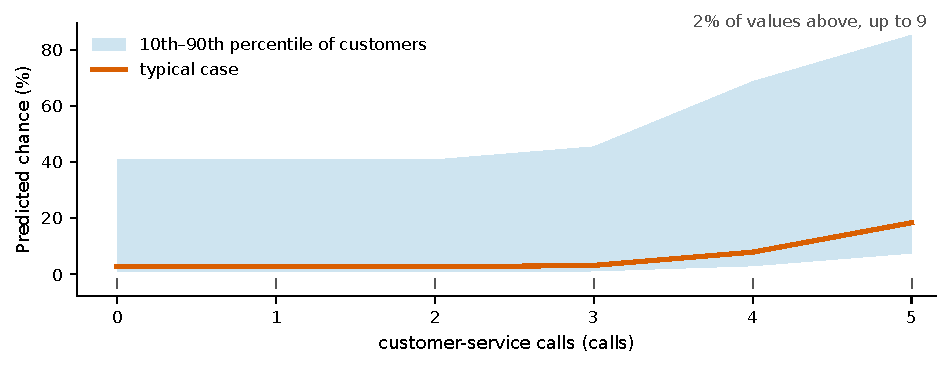
\includegraphics[width=\linewidth,height=0.88\textheight,keepaspectratio]{figures/churn100-s4-c2/ann_80-response.pdf}
\caption{Calls from 3 upwards: Response curves through this part: the typical case (bold), the 10th to 90th percentile of individual customers (band), the fold or step point (dashed) with its spread across them (grey), and the observed values (ticks).}
\label{fig:churn100s4c2:plot-ann80-0}
\end{figure}
\begin{figure}[H]\centering
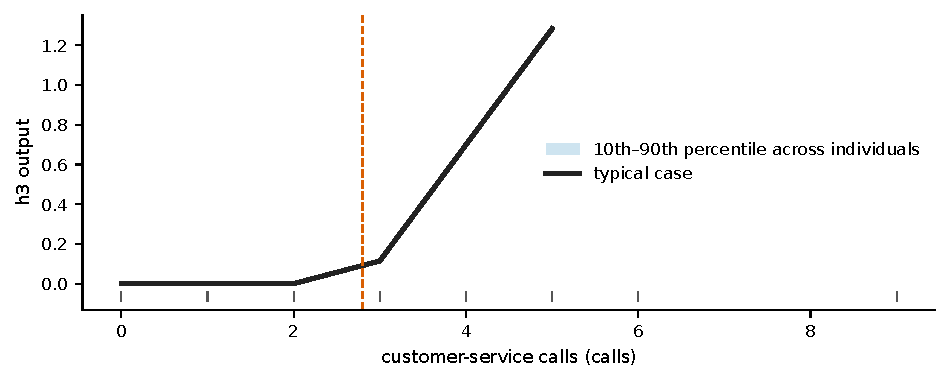
\includegraphics[width=\linewidth,height=0.88\textheight,keepaspectratio]{figures/churn100-s4-c2/ann_80-partial-5268.pdf}
\caption{Calls from 3 upwards: This part's own output, unit h3 (the output of 'Calls from 3 upwards'), on its own scale (its activation), with every other input at the typical case; it is active for 848 of 4000. Bold: the typical case; band: 10th to 90th percentile across individuals; dashed: where it switches on; ticks: the data.}
\label{fig:churn100s4c2:plot-ann80-1}
\end{figure}
\begin{figure}[H]\centering
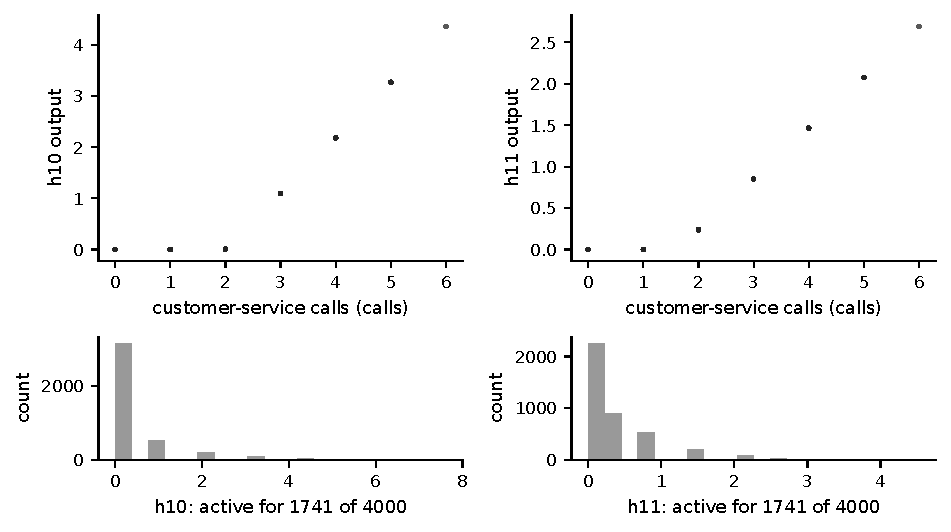
\includegraphics[width=\linewidth,height=0.88\textheight,keepaspectratio]{figures/churn100-s4-c2/ann_80-units.pdf}
\caption{Calls from 3 upwards: This part's hidden units: each unit's output against its main numeric input (top) and how often it is active (bottom).}
\label{fig:churn100s4c2:plot-ann80-2}
\end{figure}
\par\smallskip\noindent{\small Technical detail: \ref{tech:ann80}.\par}
\subsubsection{Heavy daytime use}\label{rd:ann82}
\noindent{\footnotesize Part of: The whole model (\ref{rd:ann87}).\par}
\noindent{\small Figure~\ref{fig:churn100s4c2:parts-ann82} shows what feeds this part; Figure~\ref{fig:churn100s4c2:units-ann82} its units and every connection into them (dashed boxes: connections from or to other parts, drawn in their own sections).\par}
\begin{figure}[H]\centering
\resizebox{!}{\ifdim\height>0.5\textheight 0.5\textheight\else\height\fi}{%
\resizebox{\ifdim\width>\linewidth\linewidth\else\width\fi}{!}{%
\begin{tikzpicture}[
  font=\sffamily\scriptsize, >={Stealth[length=1.6mm]},
  inp/.style={draw, rounded corners=1pt, fill=white, inner sep=1.5pt, minimum height=3.2mm, anchor=east},
  abox/.style={draw, thick, rounded corners=2pt, align=center, inner sep=3pt, minimum height=6mm, text width=42mm},
  outp/.style={draw, double, rounded corners=2pt, fill=white, align=center, inner sep=3pt, text width=24mm},
  agg/.style={draw=black!55},
]
\node[inp] (i0) at (0,1.125) {state};
\node[inp] (i1) at (0,0.375) {voice-mail messages};
\node[inp] (i2) at (0,-0.375) {total daytime minutes};
\node[inp] (i3) at (0,-1.125) {total daytime charge};
\node[outp] (out) at (9.36,0) {Heavy daytime use};
\begin{scope}[on background layer]
\draw[->, agg, thin, dashed] (i0.east) -- (out.west);
\draw[->, agg, thin, dashed] (i1.east) -- (out.west);
\draw[->, agg, thin, dashed] (i2.east) -- (out.west);
\draw[->, agg, thin, dashed] (i3.east) -- (out.west);
\end{scope}
\end{tikzpicture}}}%
\caption{Heavy daytime use: what feeds it, one level down.}
\label{fig:churn100s4c2:parts-ann82}
\end{figure}
\begin{figure}[H]\centering
\resizebox{\ifdim\width>\linewidth\linewidth\else\width\fi}{!}{%
\definecolor{netup}{HTML}{D95F02}\definecolor{netdown}{HTML}{1B9E77}\definecolor{netmixed}{HTML}{7F7F7F}%
\begin{tikzpicture}[
  font=\sffamily\scriptsize, >={Stealth[length=1.4mm]},
  inp/.style={draw, circle, fill=white, minimum size=3.2mm, inner sep=0pt},
  hid/.style={draw, circle, fill=white, minimum size=5.2mm, inner sep=0.5pt, font=\sffamily\tiny},
  exitbox/.style={draw, thick, rectangle, fill=white, align=center, text width=17mm, minimum height=5mm, inner sep=1.5pt, font=\sffamily\tiny},
  sumbox/.style={draw, thick, dashed, rectangle, fill=white, align=center, text width=17mm, minimum height=5mm, inner sep=1.5pt, font=\sffamily\tiny},
  outp/.style={draw, thick, regular polygon, regular polygon sides=6, fill=white, minimum size=10mm, inner sep=0pt, font=\sffamily\tiny, align=center},
  stub/.style={draw, dashed, rounded corners=2pt, fill=white, align=center, inner sep=2pt, font=\sffamily\tiny, text width=15mm},
  inlab/.style={font=\sffamily\tiny, align=center, text width=15mm, inner sep=1pt, fill=white, fill opacity=0.8, text opacity=1},
  wpos/.style={draw=NavyBlue}, wneg/.style={draw=BrickRed}, wagg/.style={draw=black!45, line width=1.2pt},
  wmix/.style={draw=Plum},
]
\node[hid] (n3118) at (4.35,1.9) {h2};
\node[hid] (n10131) at (2.85,1.9) {h9};
\node[inp, draw=netup, very thick] (ninxxtotalxdayxminutes) at (2.7,0.0) {};
\path (ninxxtotalxdayxminutes.south) node[inlab, anchor=north] (labninxxtotalxdayxminutes) {total daytime minutes $\uparrow$};
\node[inp, draw=netup, very thick] (ninxxtotalxdayxcharge) at (4.5,0.0) {};
\path (ninxxtotalxdayxcharge.south) node[inlab, anchor=north] (labninxxtotalxdayxcharge) {total daytime charge $\uparrow$};
\node[inp, draw=netdown, very thick] (ninxxnumberxvmailxmessages) at (6.3,0.0) {};
\path (ninxxnumberxvmailxmessages.south) node[inlab, anchor=north] (labninxxnumberxvmailxmessages) {voice-mail messages $\downarrow$};
\node[inp, draw=netmixed, very thick] (ngrpxxstate) at (0.9,0.0) {};
\path (ngrpxxstate.south) node[inlab, anchor=north] (labngrpxxstate) {state (22 of 51 used) $\updownarrow$};
\node[stub] (ntoxxthexmodelxoutput) at (3.6,3.45) {to the model output};
\begin{scope}[on background layer]
\node[fit=(n3118) (n10131) , inner sep=8pt, rounded corners=5pt, fill=Orchid!10, draw=Orchid!45] (clu0) {};
\draw[->, wpos, line width=0.44pt] (ninxxtotalxdayxminutes) -- (n3118);
\draw[->, wpos, line width=0.38pt] (ninxxtotalxdayxcharge) -- (n3118);
\draw[->, wpos, line width=0.54pt] (ninxxtotalxdayxminutes) -- (n10131);
\draw[->, wneg, line width=0.48pt] (ninxxnumberxvmailxmessages) -- (n3118);
\draw[->, wpos, line width=0.79pt] (n3118) -- (ntoxxthexmodelxoutput);
\draw[->, wpos, line width=0.92pt] (n10131) -- (ntoxxthexmodelxoutput);
\draw[->, wneg, line width=0.49pt] (ngrpxxstate) -- node[pos=0.8, sloped, above, font=\sffamily\tiny, inner sep=1pt, fill=white, fill opacity=0.8, text opacity=1] {-0.67} (n10131);
\end{scope}
\node[font=\sffamily\scriptsize\bfseries, text=Orchid!55!black, anchor=south west, inner sep=1pt, fill=white, fill opacity=0.85, text opacity=1] at (clu0.north west) {Heavy daytime use};
\end{tikzpicture}}%
\caption{Heavy daytime use: its units and every connection into them. Blue: positive weight (raises the score); red: negative weight (lowers it); thicker: larger weight. Orange outline and up arrow: raises the final prediction; teal and down arrow: lowers it; grey and double arrow: depends.}
\label{fig:churn100s4c2:units-ann82}
\end{figure}
\paragraph{Hypothesis.} This part raises the chance of leaving for heavy daytime users: daytime minutes add to it only above about 221 minutes (between 186 and 221 minutes for different customers), in an uneven way, and voice-mail messages and being in Washington lower it.\,{\scriptsize\textcolor{NavyBlue}{[C088, C080, C082]}}
\paragraph{Evidence.} This part acts on 1099 of 4000 training customers, 291 of whom left; for the typical customer it acts on, the chance is about 3\% without it and about 12\% with it.\,{\scriptsize\textcolor{NavyBlue}{[C091]}} Daytime minutes add to the chance only once they rise above about 221 minutes (between 186 and 221 minutes for different customers), in an uneven way: for a typical such customer, from about 3\% at 0 minutes to about 19\% at 271 minutes.\,{\scriptsize\textcolor{NavyBlue}{[C088]}} More voice-mail messages lower it in an uneven way: for the typical customer it acts on, from about 12\% at 0 to about 6\% at 32 messages.\,{\scriptsize\textcolor{NavyBlue}{[C080]}} Customers in Washington get less from it: about 7\% instead of about 12\% for the typical customer it acts on.\,{\scriptsize\textcolor{NavyBlue}{[C082]}} Its formula reproduces the part exactly on all 4000 training customers.\,{\scriptsize\textcolor{NavyBlue}{[C092]}}
\par\noindent{\small Evidence plots: Figure~\ref{fig:churn100s4c2:plot-ann82-0}, Figure~\ref{fig:churn100s4c2:plot-ann82-1}, Figure~\ref{fig:churn100s4c2:plot-ann82-2}, Figure~\ref{fig:churn100s4c2:plot-ann82-3}, Figure~\ref{fig:churn100s4c2:plot-ann82-4}, Figure~\ref{fig:churn100s4c2:plot-ann82-5}, Figure~\ref{fig:churn100s4c2:plot-ann82-6}, Figure~\ref{fig:churn100s4c2:plot-ann82-7}, Figure~\ref{fig:churn100s4c2:plot-ann82-8}.\par}
\par\noindent{\small Figure~\ref{fig:churn100s4c2:plot-ann82-6} shows this part's own output, unit h2: over its two main inputs, with the line where it switches on.\par}
\par\noindent{\small Figure~\ref{fig:churn100s4c2:plot-ann82-7} shows this part's own output, unit h9: it switches on at about 221.1 minutes of total daytime minutes, and is zero below.\par}
\begin{figure}[H]\centering
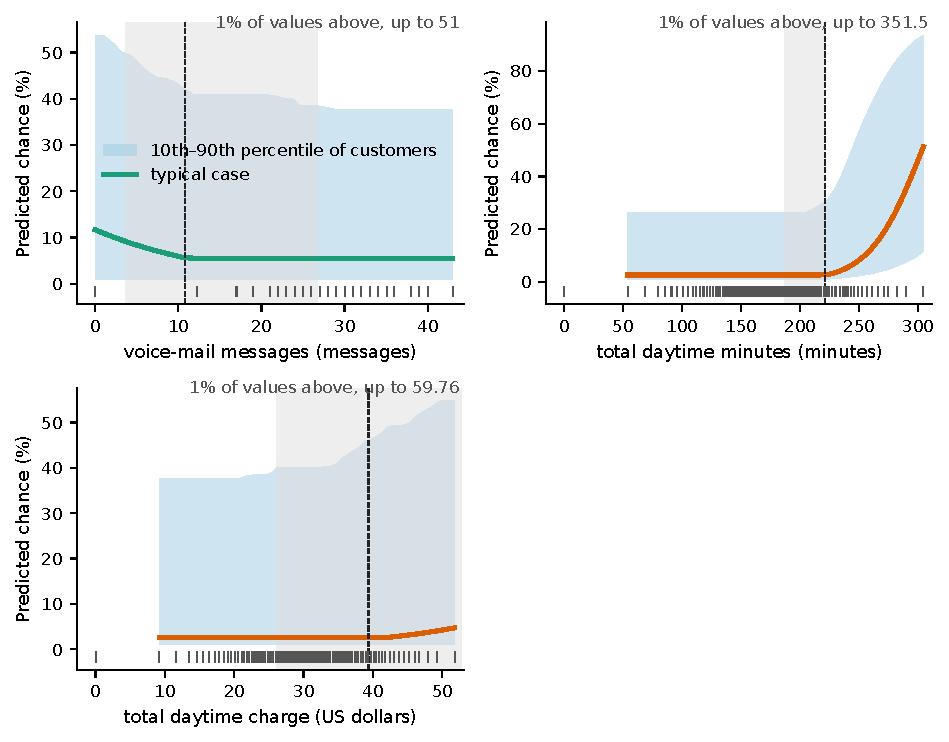
\includegraphics[width=\linewidth,height=0.88\textheight,keepaspectratio]{figures/churn100-s4-c2/ann_82-response.pdf}
\caption{Heavy daytime use: Response curves through this part: the typical case (bold), the 10th to 90th percentile of individual customers (band), the fold or step point (dashed) with its spread across them (grey), and the observed values (ticks).}
\label{fig:churn100s4c2:plot-ann82-0}
\end{figure}
\begin{figure}[H]\centering
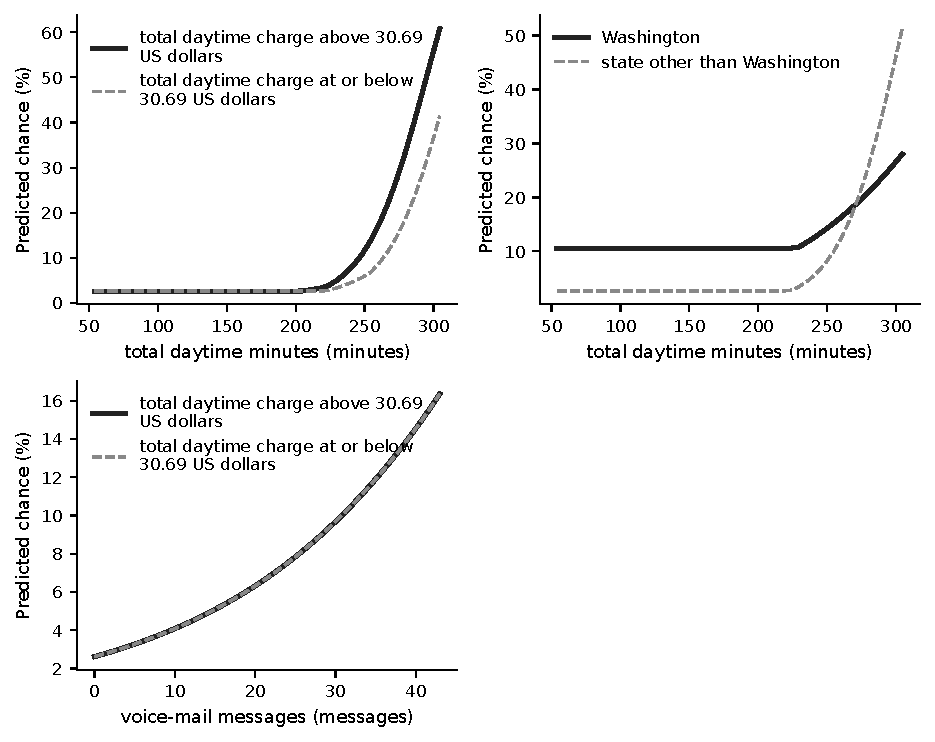
\includegraphics[width=\linewidth,height=0.88\textheight,keepaspectratio]{figures/churn100-s4-c2/ann_82-interaction.pdf}
\caption{Heavy daytime use: How the effect differs between groups: one curve per group, for the typical case of each group.}
\label{fig:churn100s4c2:plot-ann82-1}
\end{figure}
\begin{figure}[H]\centering
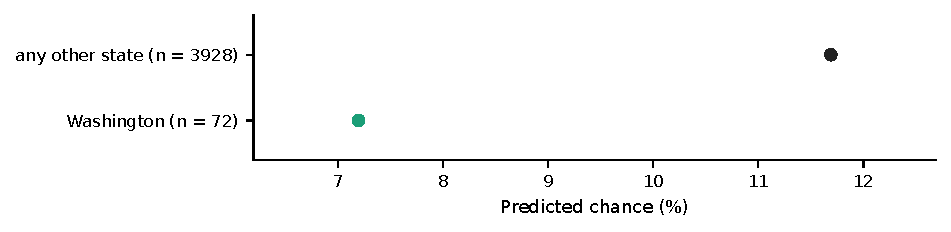
\includegraphics[width=\linewidth,height=0.88\textheight,keepaspectratio]{figures/churn100-s4-c2/ann_82-categories-small.pdf}
\caption{Heavy daytime use: The predicted value for the typical case at each level, through this part (n = training customers; grey: fewer than 20).}
\label{fig:churn100s4c2:plot-ann82-2}
\end{figure}
\begin{figure}[H]\centering
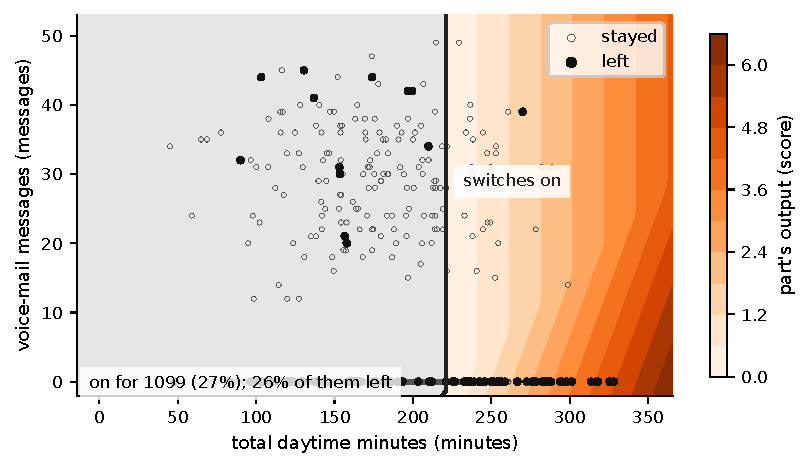
\includegraphics[width=\linewidth,height=0.88\textheight,keepaspectratio]{figures/churn100-s4-c2/ann_82-deep-map.pdf}
\caption{Heavy daytime use: The part's own output over its two numeric inputs, other inputs at the typical case: colour where it is on, flat grey where it is switched off, the black line where it switches on; training customers as hollow (no event) and filled (event) points, so the part can be seen catching the events (the predicted-chance overlay was harder to read). The switch-on line is traced on this map only; the boundary claim (C113) did not pass its check on the data, so no rule is stated.}
\label{fig:churn100s4c2:plot-ann82-3}
\end{figure}
\begin{figure}[H]\centering
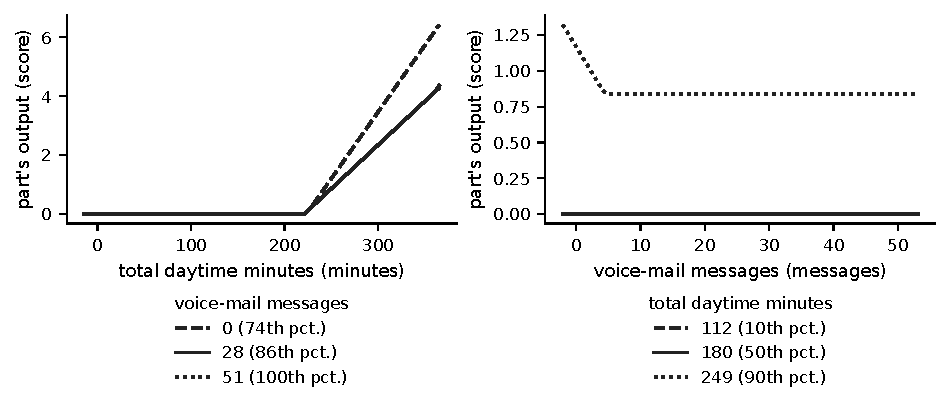
\includegraphics[width=\linewidth,height=0.88\textheight,keepaspectratio]{figures/churn100-s4-c2/ann_82-deep-slices.pdf}
\caption{Heavy daytime use: Slices of the same map: the part's own output against each input at three values of the other, so the tilted boundary shows as a shifting hinge. The switch-on line is traced on this map only; the boundary claim (C113) did not pass its check on the data, so no rule is stated.}
\label{fig:churn100s4c2:plot-ann82-4}
\end{figure}
\begin{figure}[H]\centering
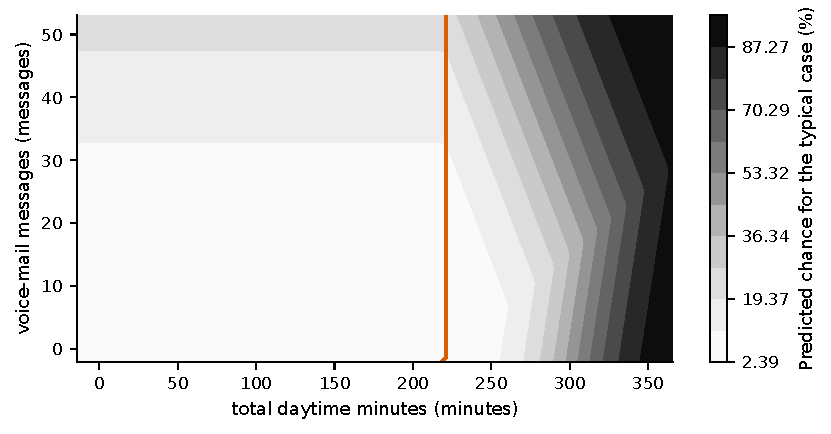
\includegraphics[width=\linewidth,height=0.88\textheight,keepaspectratio]{figures/churn100-s4-c2/ann_82-deep-risk.pdf}
\caption{Heavy daytime use: The same map on the final scale: the predicted value for the typical case, with the switch-on line (orange). The switch-on line is traced on this map only; the boundary claim (C113) did not pass its check on the data, so no rule is stated.}
\label{fig:churn100s4c2:plot-ann82-5}
\end{figure}
\begin{figure}[H]\centering
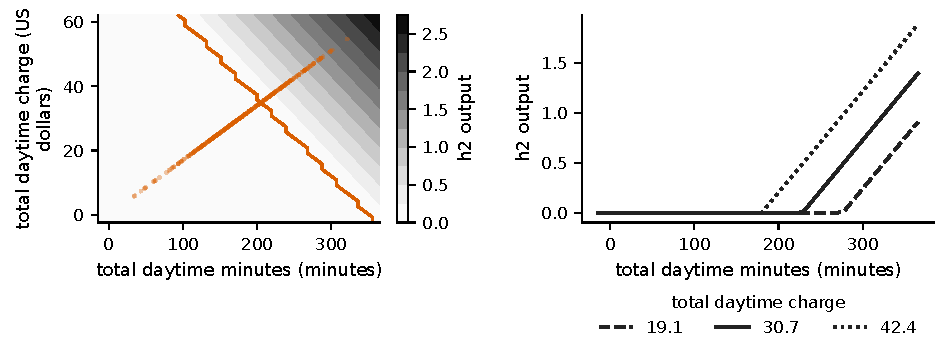
\includegraphics[width=\linewidth,height=0.88\textheight,keepaspectratio]{figures/churn100-s4-c2/ann_82-partial-3118.pdf}
\caption{Heavy daytime use: This part's own output, unit h2 (the output of 'Heavy daytime use'), on its own scale (its activation), with every other input at the typical case; it is active for 896 of 4000. Left: its output over its two main inputs (orange line: where it switches on; dots: the data); right: slices at three values of the second input.}
\label{fig:churn100s4c2:plot-ann82-6}
\end{figure}
\begin{figure}[H]\centering
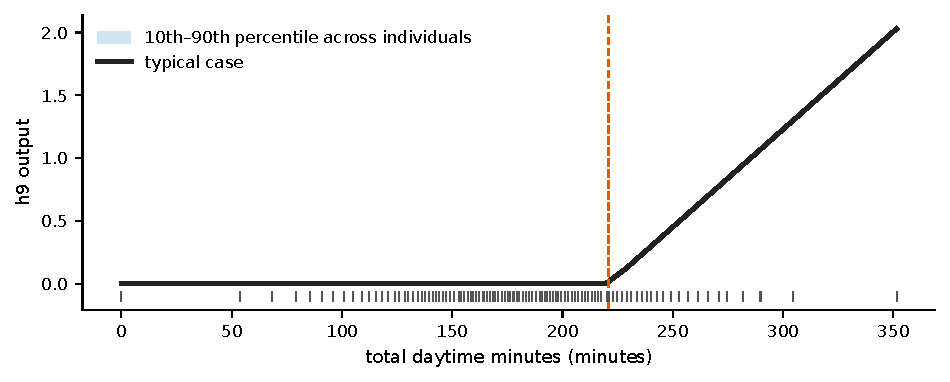
\includegraphics[width=\linewidth,height=0.88\textheight,keepaspectratio]{figures/churn100-s4-c2/ann_82-partial-10131.pdf}
\caption{Heavy daytime use: This part's own output, unit h9 (the output of 'Heavy daytime use'), on its own scale (its activation), with every other input at the typical case; it is active for 870 of 4000. Bold: the typical case; band: 10th to 90th percentile across individuals; dashed: where it switches on; ticks: the data.}
\label{fig:churn100s4c2:plot-ann82-7}
\end{figure}
\begin{figure}[H]\centering
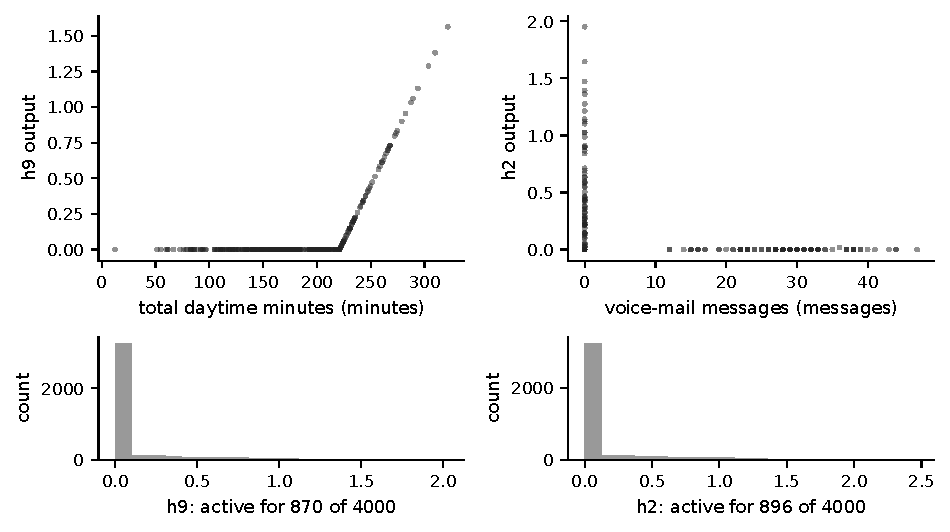
\includegraphics[width=\linewidth,height=0.88\textheight,keepaspectratio]{figures/churn100-s4-c2/ann_82-units.pdf}
\caption{Heavy daytime use: This part's hidden units: each unit's output against its main numeric input (top) and how often it is active (bottom).}
\label{fig:churn100s4c2:plot-ann82-8}
\end{figure}
\par\smallskip\noindent{\small Technical detail: \ref{tech:ann82}.\par}
\subsubsection{State units}\label{rd:ann85}
\noindent{\footnotesize Part of: The whole model (\ref{rd:ann87}).\par}
\noindent{\small Figure~\ref{fig:churn100s4c2:parts-ann85} shows what feeds this part; Figure~\ref{fig:churn100s4c2:units-ann85} its units and every connection into them (dashed boxes: connections from or to other parts, drawn in their own sections).\par}
\begin{figure}[H]\centering
\resizebox{!}{\ifdim\height>0.5\textheight 0.5\textheight\else\height\fi}{%
\resizebox{\ifdim\width>\linewidth\linewidth\else\width\fi}{!}{%
\begin{tikzpicture}[
  font=\sffamily\scriptsize, >={Stealth[length=1.6mm]},
  inp/.style={draw, rounded corners=1pt, fill=white, inner sep=1.5pt, minimum height=3.2mm, anchor=east},
  abox/.style={draw, thick, rounded corners=2pt, align=center, inner sep=3pt, minimum height=6mm, text width=42mm},
  outp/.style={draw, double, rounded corners=2pt, fill=white, align=center, inner sep=3pt, text width=24mm},
  agg/.style={draw=black!55},
]
\node[inp] (i0) at (0,-0.0) {state};
\node[outp] (out) at (9.36,0) {State units};
\begin{scope}[on background layer]
\draw[->, agg, thin, dashed] (i0.east) -- (out.west);
\end{scope}
\end{tikzpicture}}}%
\caption{State units: what feeds it, one level down.}
\label{fig:churn100s4c2:parts-ann85}
\end{figure}
\begin{figure}[H]\centering
\resizebox{\ifdim\width>\linewidth\linewidth\else\width\fi}{!}{%
\definecolor{netup}{HTML}{D95F02}\definecolor{netdown}{HTML}{1B9E77}\definecolor{netmixed}{HTML}{7F7F7F}%
\begin{tikzpicture}[
  font=\sffamily\scriptsize, >={Stealth[length=1.4mm]},
  inp/.style={draw, circle, fill=white, minimum size=3.2mm, inner sep=0pt},
  hid/.style={draw, circle, fill=white, minimum size=5.2mm, inner sep=0.5pt, font=\sffamily\tiny},
  exitbox/.style={draw, thick, rectangle, fill=white, align=center, text width=17mm, minimum height=5mm, inner sep=1.5pt, font=\sffamily\tiny},
  sumbox/.style={draw, thick, dashed, rectangle, fill=white, align=center, text width=17mm, minimum height=5mm, inner sep=1.5pt, font=\sffamily\tiny},
  outp/.style={draw, thick, regular polygon, regular polygon sides=6, fill=white, minimum size=10mm, inner sep=0pt, font=\sffamily\tiny, align=center},
  stub/.style={draw, dashed, rounded corners=2pt, fill=white, align=center, inner sep=2pt, font=\sffamily\tiny, text width=15mm},
  inlab/.style={font=\sffamily\tiny, align=center, text width=15mm, inner sep=1pt, fill=white, fill opacity=0.8, text opacity=1},
  wpos/.style={draw=NavyBlue}, wneg/.style={draw=BrickRed}, wagg/.style={draw=black!45, line width=1.2pt},
  wmix/.style={draw=Plum},
]
\node[hid] (n1295) at (0.35,1.9) {h1};
\node[hid] (n7872) at (1.1,3.25) {h6};
\node[hid] (n9954) at (1.85,1.9) {h8};
\node[inp, draw=netmixed, very thick] (ngrpxxstate) at (1.1,0.0) {};
\path (ngrpxxstate.south) node[inlab, anchor=north] (labngrpxxstate) {state (22 of 51 used) $\updownarrow$};
\node[stub] (ntoxxthexmodelxoutput) at (1.1,4.8) {to the model output};
\begin{scope}[on background layer]
\node[fit=(n1295) (n7872) (n9954) , inner sep=8pt, rounded corners=5pt, fill=Goldenrod!10, draw=Goldenrod!45] (clu0) {};
\draw[->, wpos, line width=0.61pt] (n1295) -- (n7872);
\draw[->, wneg, line width=0.60pt] (n1295) -- (ntoxxthexmodelxoutput);
\draw[->, wneg, line width=0.67pt] (n7872) -- (ntoxxthexmodelxoutput);
\draw[->, wpos, line width=0.26pt] (n9954) -- (ntoxxthexmodelxoutput);
\draw[->, wpos, line width=0.60pt] (ngrpxxstate) -- node[pos=0.8, sloped, above, font=\sffamily\tiny, inner sep=1pt, fill=white, fill opacity=0.8, text opacity=1] {+1.01} (n9954);
\draw[->, wneg, line width=0.69pt] (ngrpxxstate) -- node[pos=0.8, sloped, above, font=\sffamily\tiny, inner sep=1pt, fill=white, fill opacity=0.8, text opacity=1] {-1.27} (n1295);
\end{scope}
\node[font=\sffamily\scriptsize\bfseries, text=Goldenrod!55!black, anchor=south west, inner sep=1pt, fill=white, fill opacity=0.85, text opacity=1] at (clu0.north west) {State units};
\end{tikzpicture}}%
\caption{State units: its units and every connection into them. Blue: positive weight (raises the score); red: negative weight (lowers it); thicker: larger weight. Orange outline and up arrow: raises the final prediction; teal and down arrow: lowers it; grey and double arrow: depends.}
\label{fig:churn100s4c2:units-ann85}
\end{figure}
\paragraph{Hypothesis.} This part reads only the state and raises the chance of leaving in Rhode Island, and a little in Indiana.\,{\scriptsize\textcolor{NavyBlue}{[C100, C101]}}
\paragraph{Evidence.} Through it, a typical customer's chance goes from about 3\% to about 22\% in Rhode Island, and up by less than a point in Indiana.\,{\scriptsize\textcolor{NavyBlue}{[C100, C101]}} Its formula reproduces the part exactly on all 4000 training customers.\,{\scriptsize\textcolor{NavyBlue}{[C102]}}
\par\noindent{\small Evidence plots: Figure~\ref{fig:churn100s4c2:plot-ann85-0}, Figure~\ref{fig:churn100s4c2:plot-ann85-1}.\par}
\begin{figure}[H]\centering
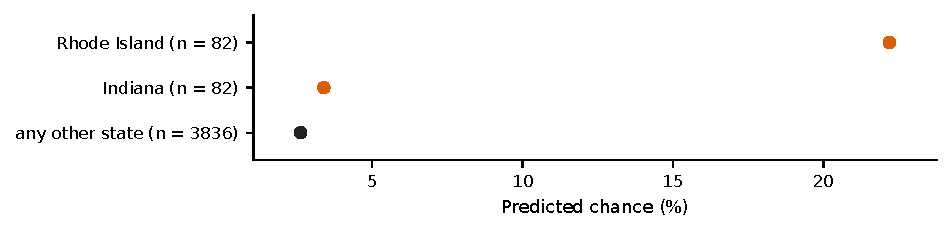
\includegraphics[width=\linewidth,height=0.88\textheight,keepaspectratio]{figures/churn100-s4-c2/ann_85-categories-small.pdf}
\caption{State units: The predicted value for the typical case at each level, through this part (n = training customers; grey: fewer than 20).}
\label{fig:churn100s4c2:plot-ann85-0}
\end{figure}
\begin{figure}[H]\centering
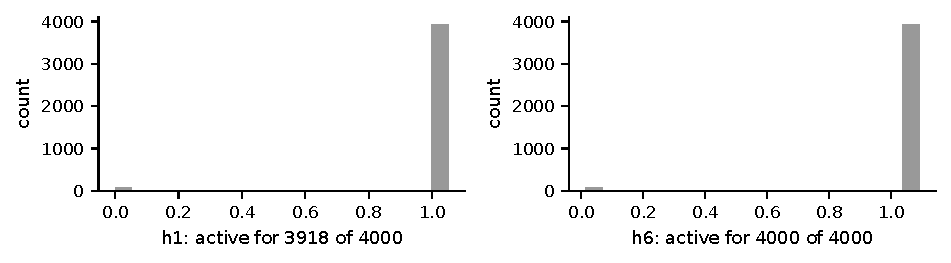
\includegraphics[width=\linewidth,height=0.88\textheight,keepaspectratio]{figures/churn100-s4-c2/ann_85-units.pdf}
\caption{State units: This part's hidden units: each unit's output against its main numeric input (top) and how often it is active (bottom).}
\label{fig:churn100s4c2:plot-ann85-1}
\end{figure}
\par\smallskip\noindent{\small Technical detail: \ref{tech:ann85}.\par}
\subsubsection{Evening unit}\label{rd:ann83}
\noindent{\footnotesize Part of: The whole model (\ref{rd:ann87}).\par}
\noindent{\small Figure~\ref{fig:churn100s4c2:parts-ann83} shows what feeds this part; Figure~\ref{fig:churn100s4c2:units-ann83} its units and every connection into them (dashed boxes: connections from or to other parts, drawn in their own sections).\par}
\begin{figure}[H]\centering
\resizebox{!}{\ifdim\height>0.5\textheight 0.5\textheight\else\height\fi}{%
\resizebox{\ifdim\width>\linewidth\linewidth\else\width\fi}{!}{%
\begin{tikzpicture}[
  font=\sffamily\scriptsize, >={Stealth[length=1.6mm]},
  inp/.style={draw, rounded corners=1pt, fill=white, inner sep=1.5pt, minimum height=3.2mm, anchor=east},
  abox/.style={draw, thick, rounded corners=2pt, align=center, inner sep=3pt, minimum height=6mm, text width=42mm},
  outp/.style={draw, double, rounded corners=2pt, fill=white, align=center, inner sep=3pt, text width=24mm},
  agg/.style={draw=black!55},
]
\node[inp] (i0) at (0,-0.0) {total evening minutes};
\node[outp] (out) at (9.36,0) {Evening unit};
\begin{scope}[on background layer]
\draw[->, agg, thin, dashed] (i0.east) -- (out.west);
\end{scope}
\end{tikzpicture}}}%
\caption{Evening unit: what feeds it, one level down.}
\label{fig:churn100s4c2:parts-ann83}
\end{figure}
\begin{figure}[H]\centering
\resizebox{\ifdim\width>\linewidth\linewidth\else\width\fi}{!}{%
\definecolor{netup}{HTML}{D95F02}\definecolor{netdown}{HTML}{1B9E77}\definecolor{netmixed}{HTML}{7F7F7F}%
\begin{tikzpicture}[
  font=\sffamily\scriptsize, >={Stealth[length=1.4mm]},
  inp/.style={draw, circle, fill=white, minimum size=3.2mm, inner sep=0pt},
  hid/.style={draw, circle, fill=white, minimum size=5.2mm, inner sep=0.5pt, font=\sffamily\tiny},
  exitbox/.style={draw, thick, rectangle, fill=white, align=center, text width=17mm, minimum height=5mm, inner sep=1.5pt, font=\sffamily\tiny},
  sumbox/.style={draw, thick, dashed, rectangle, fill=white, align=center, text width=17mm, minimum height=5mm, inner sep=1.5pt, font=\sffamily\tiny},
  outp/.style={draw, thick, regular polygon, regular polygon sides=6, fill=white, minimum size=10mm, inner sep=0pt, font=\sffamily\tiny, align=center},
  stub/.style={draw, dashed, rounded corners=2pt, fill=white, align=center, inner sep=2pt, font=\sffamily\tiny, text width=15mm},
  inlab/.style={font=\sffamily\tiny, align=center, text width=15mm, inner sep=1pt, fill=white, fill opacity=0.8, text opacity=1},
  wpos/.style={draw=NavyBlue}, wneg/.style={draw=BrickRed}, wagg/.style={draw=black!45, line width=1.2pt},
  wmix/.style={draw=Plum},
]
\node[exitbox] (n15524) at (1.2,3.25) {Evening unit $\uparrow$};
\node[hid] (n14484) at (1.2,1.9) {h12};
\node[inp, draw=netup, very thick] (ninxxtotalxevexminutes) at (1.2,0.0) {};
\path (ninxxtotalxevexminutes.south) node[inlab, anchor=north] (labninxxtotalxevexminutes) {total evening minutes $\uparrow$};
\node[stub] (ntoxxthexmodelxoutput) at (1.2,4.8) {to the model output};
\begin{scope}[on background layer]
\node[fit=(n15524) (n14484) , inner sep=8pt, rounded corners=5pt, fill=Cerulean!10, draw=Cerulean!45] (clu0) {};
\draw[->, wpos, line width=0.60pt] (ninxxtotalxevexminutes) -- (n14484);
\draw[->, wpos, line width=0.61pt] (n14484) -- (n15524);
\draw[->, wpos, line width=0.32pt] (n15524) -- (ntoxxthexmodelxoutput);
\end{scope}
\node[font=\sffamily\scriptsize\bfseries, text=Cerulean!55!black, anchor=south west, inner sep=1pt, fill=white, fill opacity=0.85, text opacity=1] at (clu0.north west) {Evening unit};
\end{tikzpicture}}%
\caption{Evening unit: its units and every connection into them. Blue: positive weight (raises the score); red: negative weight (lowers it); thicker: larger weight. Orange outline and up arrow: raises the final prediction; teal and down arrow: lowers it; grey and double arrow: depends.}
\label{fig:churn100s4c2:units-ann83}
\end{figure}
\paragraph{Hypothesis.} This part reads evening minutes and barely changes the chance of leaving: nothing until about 217 minutes, then steadily.\,{\scriptsize\textcolor{NavyBlue}{[C103, C104]}}
\paragraph{Evidence.} Through it, evening minutes change nothing until about 217 minutes, then raise the chance steadily, but a typical customer's chance stays at about 3\% from 138 to 266 minutes.\,{\scriptsize\textcolor{NavyBlue}{[C103]}} Its formula reproduces the part exactly on all 4000 training customers.\,{\scriptsize\textcolor{NavyBlue}{[C105]}}
\par\noindent{\small Evidence plots: Figure~\ref{fig:churn100s4c2:plot-ann83-0}, Figure~\ref{fig:churn100s4c2:plot-ann83-1}.\par}
\begin{figure}[H]\centering
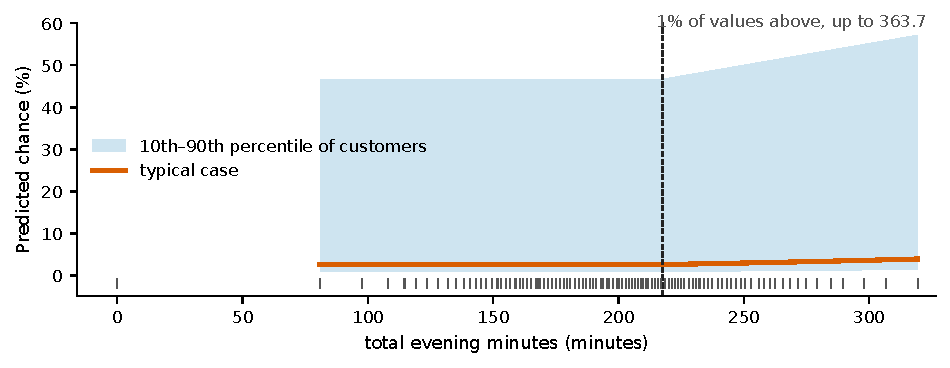
\includegraphics[width=\linewidth,height=0.88\textheight,keepaspectratio]{figures/churn100-s4-c2/ann_83-response.pdf}
\caption{Evening unit: Response curves through this part: the typical case (bold), the 10th to 90th percentile of individual customers (band), the fold or step point (dashed) with its spread across them (grey), and the observed values (ticks).}
\label{fig:churn100s4c2:plot-ann83-0}
\end{figure}
\begin{figure}[H]\centering
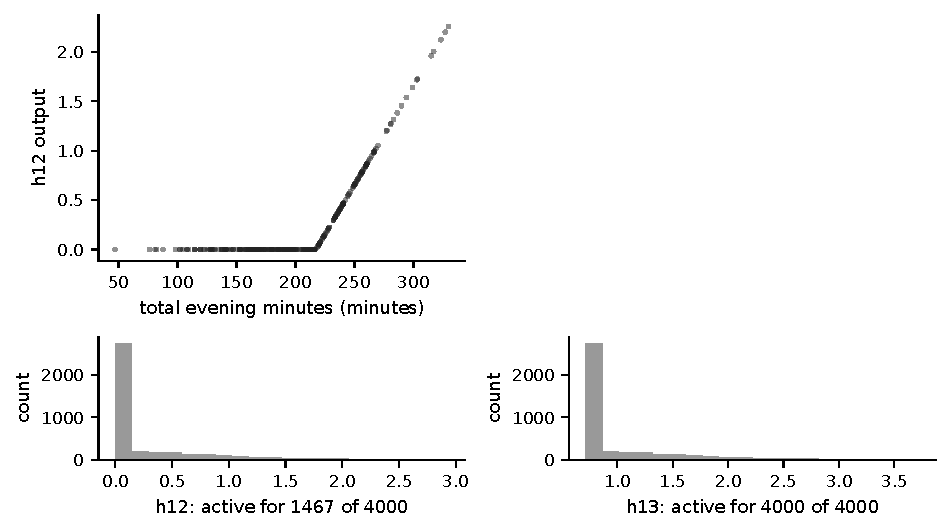
\includegraphics[width=\linewidth,height=0.88\textheight,keepaspectratio]{figures/churn100-s4-c2/ann_83-units.pdf}
\caption{Evening unit: This part's hidden units: each unit's output against its main numeric input (top) and how often it is active (bottom).}
\label{fig:churn100s4c2:plot-ann83-1}
\end{figure}
\par\smallskip\noindent{\small Technical detail: \ref{tech:ann83}.\par}
\subsubsection{Small voice-mail unit}\label{rd:ann84}
\noindent{\footnotesize Part of: The whole model (\ref{rd:ann87}).\par}
\noindent{\small Figure~\ref{fig:churn100s4c2:parts-ann84} shows what feeds this part; Figure~\ref{fig:churn100s4c2:units-ann84} its units and every connection into them (dashed boxes: connections from or to other parts, drawn in their own sections).\par}
\begin{figure}[H]\centering
\resizebox{!}{\ifdim\height>0.5\textheight 0.5\textheight\else\height\fi}{%
\resizebox{\ifdim\width>\linewidth\linewidth\else\width\fi}{!}{%
\begin{tikzpicture}[
  font=\sffamily\scriptsize, >={Stealth[length=1.6mm]},
  inp/.style={draw, rounded corners=1pt, fill=white, inner sep=1.5pt, minimum height=3.2mm, anchor=east},
  abox/.style={draw, thick, rounded corners=2pt, align=center, inner sep=3pt, minimum height=6mm, text width=42mm},
  outp/.style={draw, double, rounded corners=2pt, fill=white, align=center, inner sep=3pt, text width=24mm},
  agg/.style={draw=black!55},
]
\node[inp] (i0) at (0,0.375) {state};
\node[inp] (i1) at (0,-0.375) {voice-mail messages};
\node[outp] (out) at (9.36,0) {Small voice-mail unit};
\begin{scope}[on background layer]
\draw[->, agg, thin, dashed] (i0.east) -- (out.west);
\draw[->, agg, thin, dashed] (i1.east) -- (out.west);
\end{scope}
\end{tikzpicture}}}%
\caption{Small voice-mail unit: what feeds it, one level down.}
\label{fig:churn100s4c2:parts-ann84}
\end{figure}
\begin{figure}[H]\centering
\resizebox{\ifdim\width>\linewidth\linewidth\else\width\fi}{!}{%
\definecolor{netup}{HTML}{D95F02}\definecolor{netdown}{HTML}{1B9E77}\definecolor{netmixed}{HTML}{7F7F7F}%
\begin{tikzpicture}[
  font=\sffamily\scriptsize, >={Stealth[length=1.4mm]},
  inp/.style={draw, circle, fill=white, minimum size=3.2mm, inner sep=0pt},
  hid/.style={draw, circle, fill=white, minimum size=5.2mm, inner sep=0.5pt, font=\sffamily\tiny},
  exitbox/.style={draw, thick, rectangle, fill=white, align=center, text width=17mm, minimum height=5mm, inner sep=1.5pt, font=\sffamily\tiny},
  sumbox/.style={draw, thick, dashed, rectangle, fill=white, align=center, text width=17mm, minimum height=5mm, inner sep=1.5pt, font=\sffamily\tiny},
  outp/.style={draw, thick, regular polygon, regular polygon sides=6, fill=white, minimum size=10mm, inner sep=0pt, font=\sffamily\tiny, align=center},
  stub/.style={draw, dashed, rounded corners=2pt, fill=white, align=center, inner sep=2pt, font=\sffamily\tiny, text width=15mm},
  inlab/.style={font=\sffamily\tiny, align=center, text width=15mm, inner sep=1pt, fill=white, fill opacity=0.8, text opacity=1},
  wpos/.style={draw=NavyBlue}, wneg/.style={draw=BrickRed}, wagg/.style={draw=black!45, line width=1.2pt},
  wmix/.style={draw=Plum},
]
\node[exitbox] (n6089) at (2.1,1.9) {Small voice-mail unit $\uparrow$};
\node[inp, draw=netup, very thick] (ninxxnumberxvmailxmessages) at (3.0,0.0) {};
\path (ninxxnumberxvmailxmessages.south) node[inlab, anchor=north] (labninxxnumberxvmailxmessages) {voice-mail messages $\uparrow$};
\node[inp, draw=netmixed, very thick] (ngrpxxstate) at (1.2,0.0) {};
\path (ngrpxxstate.south) node[inlab, anchor=north] (labngrpxxstate) {state (22 of 51 used) $\updownarrow$};
\node[stub] (ntoxxthexmodelxoutput) at (2.1,3.45) {to the model output};
\begin{scope}[on background layer]
\node[fit=(n6089) , inner sep=8pt, rounded corners=5pt, fill=Mahogany!10, draw=Mahogany!45] (clu0) {};
\draw[->, wpos, line width=0.54pt] (ninxxnumberxvmailxmessages) -- (n6089);
\draw[->, wpos, line width=0.25pt] (n6089) -- (ntoxxthexmodelxoutput);
\draw[->, wpos, line width=0.65pt] (ngrpxxstate) -- node[pos=0.8, sloped, above, font=\sffamily\tiny, inner sep=1pt, fill=white, fill opacity=0.8, text opacity=1] {+1.14} (n6089);
\end{scope}
\node[font=\sffamily\scriptsize\bfseries, text=Mahogany!55!black, anchor=south west, inner sep=1pt, fill=white, fill opacity=0.85, text opacity=1] at (clu0.north west) {Small voice-mail unit};
\end{tikzpicture}}%
\caption{Small voice-mail unit: its units and every connection into them. Blue: positive weight (raises the score); red: negative weight (lowers it); thicker: larger weight. Orange outline and up arrow: raises the final prediction; teal and down arrow: lowers it; grey and double arrow: depends.}
\label{fig:churn100s4c2:units-ann84}
\end{figure}
\paragraph{Hypothesis.} This small part reads voice-mail messages and being in Louisiana, and barely changes the predictions.\,{\scriptsize\textcolor{NavyBlue}{[C111]}}
\paragraph{Evidence.} Through it, a typical customer's chance stays at about 3\% in Louisiana as elsewhere, and voice-mail messages barely change it (about 3\% at 0 and at 32 messages).\,{\scriptsize\textcolor{NavyBlue}{[C106, C107]}} Switching it off changes the predictions by at most one point.\,{\scriptsize\textcolor{NavyBlue}{[C111]}} Its formula reproduces the part exactly on all 4000 training customers.\,{\scriptsize\textcolor{NavyBlue}{[C112]}}
\par\noindent{\small Evidence plots: Figure~\ref{fig:churn100s4c2:plot-ann84-0}, Figure~\ref{fig:churn100s4c2:plot-ann84-1}, Figure~\ref{fig:churn100s4c2:plot-ann84-2}, Figure~\ref{fig:churn100s4c2:plot-ann84-3}.\par}
\begin{figure}[H]\centering
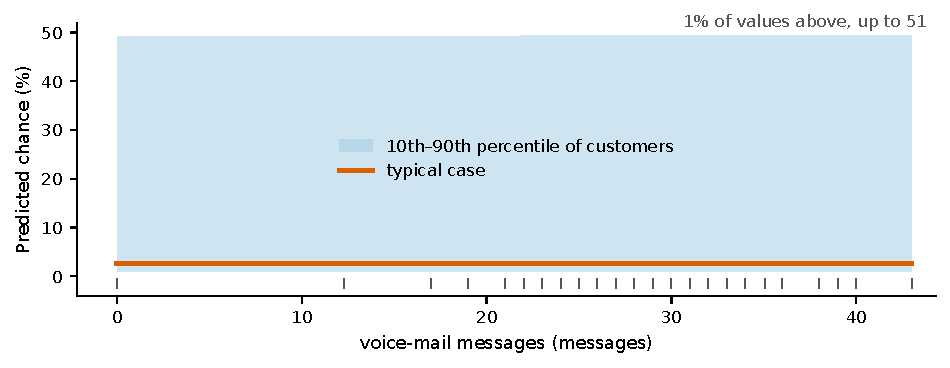
\includegraphics[width=\linewidth,height=0.88\textheight,keepaspectratio]{figures/churn100-s4-c2/ann_84-response.pdf}
\caption{Small voice-mail unit: Response curves through this part: the typical case (bold), the 10th to 90th percentile of individual customers (band), the fold or step point (dashed) with its spread across them (grey), and the observed values (ticks).}
\label{fig:churn100s4c2:plot-ann84-0}
\end{figure}
\begin{figure}[H]\centering
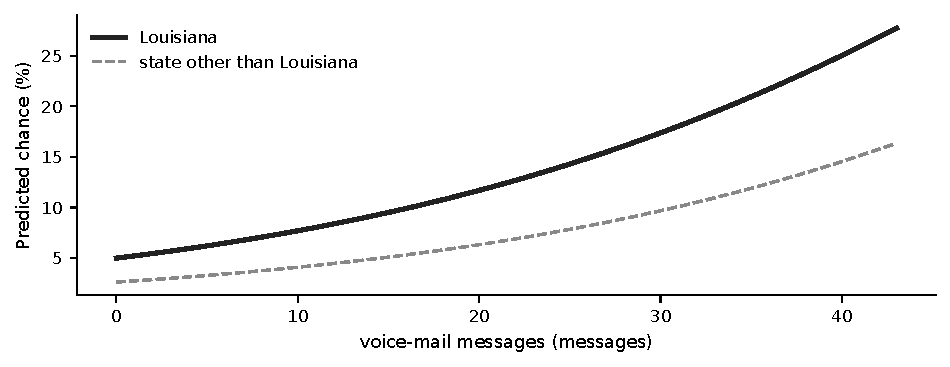
\includegraphics[width=\linewidth,height=0.88\textheight,keepaspectratio]{figures/churn100-s4-c2/ann_84-interaction.pdf}
\caption{Small voice-mail unit: How the effect differs between groups: one curve per group, for the typical case of each group.}
\label{fig:churn100s4c2:plot-ann84-1}
\end{figure}
\begin{figure}[H]\centering
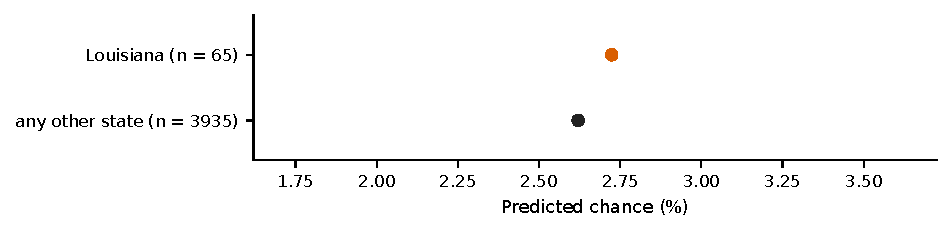
\includegraphics[width=\linewidth,height=0.88\textheight,keepaspectratio]{figures/churn100-s4-c2/ann_84-categories-small.pdf}
\caption{Small voice-mail unit: The predicted value for the typical case at each level, through this part (n = training customers; grey: fewer than 20).}
\label{fig:churn100s4c2:plot-ann84-2}
\end{figure}
\begin{figure}[H]\centering
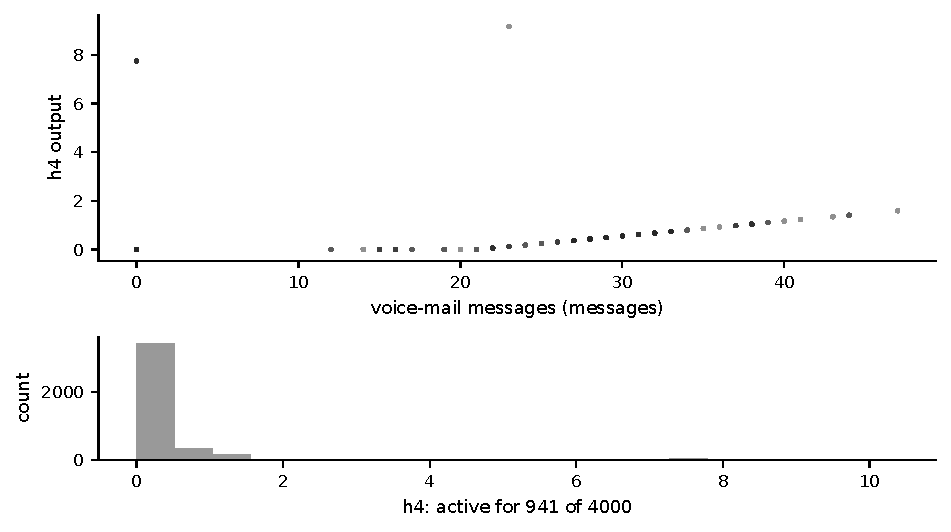
\includegraphics[width=\linewidth,height=0.88\textheight,keepaspectratio]{figures/churn100-s4-c2/ann_84-units.pdf}
\caption{Small voice-mail unit: This part's hidden units: each unit's output against its main numeric input (top) and how often it is active (bottom).}
\label{fig:churn100s4c2:plot-ann84-3}
\end{figure}
\par\smallskip\noindent{\small Technical detail: \ref{tech:ann84}.\par}
\subsection{Not supported by the model}
\begin{itemize}\setlength\itemsep{0pt}\small
\item C109: threshold claim about number of voice-mail messages in part ann\_\allowbreak{}84: not supported by the model (the fold changes the curve by only 0.007 log-odds compared with a straight line (needed 0.1); the effect past the fold is too small or not consistent across patients).
\item C110: subgroup claim about state and number of voice-mail messages in part ann\_\allowbreak{}84: not supported by the model (its effect is negligible).
\item C113: boundary claim about total daytime minutes and number of voice-mail messages in part ann\_\allowbreak{}82: not supported by the model (the boundary rule matches 0.0 of training rows (needs 0.99)).
\end{itemize}
\clearpage\section*{Technical detail: churn100-s4-c2}
\addcontentsline{toc}{section}{Technical detail: churn100-s4-c2}
\noindent{\small The record behind each part: the original hypothesis, the closed form, and every claim with its estimate (log-odds and odds ratio), range across patients, n and test check.\par}
\renewcommand{\thesubsection}{T.\arabic{subsection}}\setcounter{subsection}{0}
\subsection{The whole model}\label{tech:ann87}
\noindent{\footnotesize Annotation ann\_\allowbreak{}87 (churn\_\allowbreak{}logit). Reads: state, account length, area code, international calling plan, voice-mail plan, number of voice-mail messages, total daytime minutes, total daytime calls, total daytime charge, total evening minutes, total evening calls, total evening charge, total night-time minutes, total night-time calls, total night-time charge, total international minutes, total international calls, total international charge, number of calls to customer service.\par}
\paragraph{Original hypothesis (unchanged).} Root: logit P(churn) = -1.30 + linear\_\allowbreak{}backbone (identity\_\allowbreak{}lin) + service\_\allowbreak{}calls (identity\_\allowbreak{}svc) + 1.53*3118 + 1.91*10131 (day\_\allowbreak{}usage\_\allowbreak{}hinges) + 0.20*15524 (evening\_\allowbreak{}hinge) - 1.01*1295 - 1.21*7872 + 0.04*9954 (state\_\allowbreak{}offsets) + 0.005*6089, purely additive in the logit; the sigmoid is the only coupling. 37 inputs are unconnected (international charge and calls, night minutes/\allowbreak{}charge/\allowbreak{}calls,\allowbreak{} evening calls, area codes 408/510 and 29 state indicators) and have zero effect. Train AUC 0.8908, accuracy 0.888. Performance sources (train): all children replaced by least-squares linear fits gives AUC 0.8333 (an L2 logistic regression refit on all 71 inputs gets 0.8433); restoring day\_\allowbreak{}usage\_\allowbreak{}hinges alone gives 0.8707, service\_\allowbreak{}calls alone 0.8659, both 0.8907; evening, state and voicemail units restore nothing. So the gain over linear (+0.058) comes from the day-usage and service-call thresholds, which are complementary. Rare-category switches: state:11 -2.75 logit (73 rows, empirical -1.35); state:46 -1.94 (80 rows, -0.91); state:45 -0.94 (91, -0.85); state:47 +0.90 mean (72 rows, empirical +0.92; direct +1.23, but it switches off 10131 so heavy day users lose up to 2.75); state:31 +0.83 (90, +0.67); state:18 +0.41 (65 rows, empirical -0.48: opposite sign); state:39 -0.25 net (82, -0.93: direct -2.61 almost cancelled by the state units).
\paragraph{Closed form.} Read through its parts (their formulas are in their own sections).
\paragraph{Split inputs.} To annotate the parts, the explanation split these inputs into copies (a refactoring step that does not change what the model computes); the diagrams draw each input once: customer-service calls (2 copies); voice-mail messages (3 copies).
\paragraph{State: every level the model reads.} Whole-model change in the predicted chance for a typical customer when only the state changes from the reference; n = training customers in that level.\par\smallskip
{\scriptsize\rowcolors{2}{black!6}{white}
\begin{longtable}{@{}lllrlc@{}}
\toprule\rowcolor{white}
Claim & From & To & n & Chance & OK \\
\midrule\endhead
\bottomrule\endfoot
C002 & West Virginia & Washington & 72 & 3\% to 11\% & \textcolor{OliveGreen}{yes} \\
C005 & West Virginia & New Jersey & 90 & 3\% to 7\% & \textcolor{OliveGreen}{yes} \\
C008 & West Virginia & Louisiana & 65 & 3\% to 5\% & \textcolor{OliveGreen}{yes} \\
C009 & West Virginia & Connecticut & 80 & 3\% to 5\% & \textcolor{OliveGreen}{yes} \\
C013 & West Virginia & Tennessee & 68 & 3\% to 5\% & \textcolor{OliveGreen}{yes} \\
C014 & West Virginia & Massachusetts & 86 & 3\% to 5\% & \textcolor{OliveGreen}{yes} \\
C015 & West Virginia & Oregon & 84 & 3\% to 4\% & \textcolor{OliveGreen}{yes} \\
C016 & West Virginia & Indiana & 82 & 3\% to 4\% & \textcolor{OliveGreen}{yes} \\
C017 & West Virginia & Kentucky & 81 & 3\% to 4\% & \textcolor{OliveGreen}{yes} \\
C019 & West Virginia & South Dakota & 66 & 3\% to 4\% & \textcolor{OliveGreen}{yes} \\
C020 & West Virginia & Oklahoma & 79 & 3\% to 4\% & \textcolor{OliveGreen}{yes} \\
C024 & West Virginia & North Dakota & 68 & 3\% to 3\% & \textcolor{OliveGreen}{yes} \\
C025 & West Virginia & state other than Georgia, Hawaii, Indiana, Kentucky, Loui... & 2286 & 3\% to 3\% & \textcolor{OliveGreen}{yes} \\
C027 & West Virginia & Arizona & 73 & 3\% to 3\% & \textcolor{OliveGreen}{yes} \\
C030 & West Virginia & Arkansas & 78 & 3\% to 3\% & \textcolor{OliveGreen}{yes} \\
C033 & West Virginia & Rhode Island & 82 & 3\% to 3\% & \textcolor{OliveGreen}{yes} \\
C034 & West Virginia & Florida & 78 & 3\% to 3\% & \textcolor{OliveGreen}{yes} \\
C023 & West Virginia & Pennsylvania & 56 & 3\% to 2\% & \textcolor{OliveGreen}{yes} \\
C022 & West Virginia & Georgia & 60 & 3\% to 2\% & \textcolor{OliveGreen}{yes} \\
C018 & West Virginia & Virginia & 91 & 3\% to 1\% & \textcolor{OliveGreen}{yes} \\
C012 & West Virginia & Vermont & 80 & 3\% to $<$1\% & \textcolor{OliveGreen}{yes} \\
C007 & West Virginia & Hawaii & 73 & 3\% to $<$1\% & \textcolor{OliveGreen}{yes} \\
\end{longtable}}
\paragraph{Evidence table} (next page, landscape).
\begin{landscape}
{\scriptsize\setlength{\tabcolsep}{3pt}\renewcommand{\arraystretch}{1.15}
\rowcolors{2}{black!6}{white}
\begin{longtable}{@{}l>{\raggedright\arraybackslash}p{0.36\linewidth}>{\raggedright\arraybackslash}p{0.14\linewidth}rrr>{\raggedright\arraybackslash}p{0.06\linewidth}>{\raggedright\arraybackslash}p{0.17\linewidth}c@{}}
\toprule\rowcolor{white}
ID & What is checked & Risk, typical patient & Log-odds & OR & Range (p10--p90) & n & Test check & OK \\
\midrule\endfirsthead
\toprule\rowcolor{white}
ID & What is checked & Risk, typical patient & Log-odds & OR & Range (p10--p90) & n & Test check & OK \\
\midrule\endhead
\bottomrule\endfoot
C001 & direction: international calling plan: no international plan to an international plan (whole model) \newline{\itshape shape: categorical; highest to lowest: an international plan, no international plan} & 3\% to 31\% & 2.82 & 16.7 & 2.82 to 2.82 & 3620, 380 & agrees; AUC gain 0.060 [0.032, 0.090] & \textcolor{OliveGreen}{yes} \\
C002 & direction: state: West Virginia to Washington (whole model) \newline{\itshape shape: categorical; highest to lowest: Washington, New Jersey, Louisiana, Connecticut, Tennessee, Massachusetts ...} & 3\% to 11\% & 1.27 & 3.58 & 0.64 to 1.48 & 122, 72 & disagrees; AUC gain -0.012 [-0.026, 0.0005] & \textcolor{OliveGreen}{yes} \\
C003 & direction: voice-mail messages: 0 messages to 32 messages (whole model) \newline{\itshape shape: steady; 72\% of patients same; fallback; risk saturates near 0\%} & 3\% to 11\% & 1.21 & 3.35 & 0.39 to 1.47 & 4000 & agrees; AUC gain 0.017 [0.005, 0.031] & \textcolor{OliveGreen}{yes} \\
C004 & direction: total daytime minutes: 112 minutes to 249 minutes (whole model) \newline{\itshape shape: hinge at 223 minutes; 50\% of patients same; fallback; risk saturates near 0\%; matches the fold at 221 minutes} & 3\% to 8\% & 1.13 & 3.10 & 0.83 to 1.79 & 4000 & agrees; AUC gain 0.036 [0.015, 0.059] & \textcolor{OliveGreen}{yes} \\
C005 & direction: state: West Virginia to New Jersey (whole model) \newline{\itshape shape: categorical; highest to lowest: Washington, New Jersey, Louisiana, Connecticut, Tennessee, Massachusetts ...} & 3\% to 7\% & 1.09 & 2.97 & 1.09 to 1.09 & 122, 90 & disagrees; AUC gain -0.012 [-0.026, 0.0005] & \textcolor{OliveGreen}{yes} \\
C006 & direction: voice-mail plan: no voice-mail plan to a voice-mail plan (whole model) \newline{\itshape shape: categorical; highest to lowest: no voice-mail plan, a voice-mail plan} & 3\% to $<$1\% & -2.54 & 0.08 & -2.54 to -2.54 & 2939, 1061 & agrees; AUC gain 0.033 [0.014, 0.053] & \textcolor{OliveGreen}{yes} \\
C007 & direction: state: West Virginia to Hawaii (whole model) \newline{\itshape shape: categorical; highest to lowest: Washington, New Jersey, Louisiana, Connecticut, Tennessee, Massachusetts ...} & 3\% to $<$1\% & -2.50 & 0.08 & -2.50 to -2.50 & 122, 73 & disagrees; AUC gain -0.012 [-0.026, 0.0005] & \textcolor{OliveGreen}{yes} \\
C008 & direction: state: West Virginia to Louisiana (whole model) \newline{\itshape shape: categorical; highest to lowest: Washington, New Jersey, Louisiana, Connecticut, Tennessee, Massachusetts ...} & 3\% to 5\% & 0.67 & 1.95 & 0.67 to 0.67 & 122, 65 & disagrees; AUC gain -0.012 [-0.026, 0.0005] & \textcolor{OliveGreen}{yes} \\
C009 & direction: state: West Virginia to Connecticut (whole model) \newline{\itshape shape: categorical; highest to lowest: Washington, New Jersey, Louisiana, Connecticut, Tennessee, Massachusetts ...} & 3\% to 5\% & 0.66 & 1.94 & 0.66 to 0.66 & 122, 80 & disagrees; AUC gain -0.012 [-0.026, 0.0005] & \textcolor{OliveGreen}{yes} \\
C010 & direction: total evening charge: 11.76 US dollars to 22.57 US dollars (whole model) \newline{\itshape shape: steady; 100\% of patients same; verified; risk saturates near 0\%} & 2\% to 4\% & 0.88 & 2.42 & 0.88 to 0.88 & 4000 & agrees; AUC gain 0.013 [0.004, 0.022] & \textcolor{OliveGreen}{yes} \\
C011 & direction: total international minutes: 7 minutes to 14 minutes (whole model) \newline{\itshape shape: steady; 100\% of patients same; verified; risk saturates near 0\%} & 2\% to 4\% & 0.85 & 2.35 & 0.85 to 0.85 & 4000 & unclear; AUC gain 0.0008 [-0.007, 0.008] & \textcolor{OliveGreen}{yes} \\
C012 & direction: state: West Virginia to Vermont (whole model) \newline{\itshape shape: categorical; highest to lowest: Washington, New Jersey, Louisiana, Connecticut, Tennessee, Massachusetts ...} & 3\% to $<$1\% & -1.68 & 0.19 & -1.68 to -1.68 & 122, 80 & disagrees; AUC gain -0.012 [-0.026, 0.0005] & \textcolor{OliveGreen}{yes} \\
C013 & direction: state: West Virginia to Tennessee (whole model) \newline{\itshape shape: categorical; highest to lowest: Washington, New Jersey, Louisiana, Connecticut, Tennessee, Massachusetts ...} & 3\% to 5\% & 0.60 & 1.82 & 0.60 to 0.60 & 122, 68 & disagrees; AUC gain -0.012 [-0.026, 0.0005] & \textcolor{OliveGreen}{yes} \\
C014 & direction: state: West Virginia to Massachusetts (whole model) \newline{\itshape shape: categorical; highest to lowest: Washington, New Jersey, Louisiana, Connecticut, Tennessee, Massachusetts ...} & 3\% to 5\% & 0.57 & 1.77 & 0.57 to 0.57 & 122, 86 & disagrees; AUC gain -0.012 [-0.026, 0.0005] & \textcolor{OliveGreen}{yes} \\
C015 & direction: state: West Virginia to Oregon (whole model) \newline{\itshape shape: categorical; highest to lowest: Washington, New Jersey, Louisiana, Connecticut, Tennessee, Massachusetts ...} & 3\% to 4\% & 0.53 & 1.70 & 0.53 to 0.53 & 122, 84 & disagrees; AUC gain -0.012 [-0.026, 0.0005] & \textcolor{OliveGreen}{yes} \\
C016 & direction: state: West Virginia to Indiana (whole model) \newline{\itshape shape: categorical; highest to lowest: Washington, New Jersey, Louisiana, Connecticut, Tennessee, Massachusetts ...} & 3\% to 4\% & 0.52 & 1.69 & 0.52 to 0.52 & 122, 82 & disagrees; AUC gain -0.012 [-0.026, 0.0005] & \textcolor{OliveGreen}{yes} \\
C017 & direction: state: West Virginia to Kentucky (whole model) \newline{\itshape shape: categorical; highest to lowest: Washington, New Jersey, Louisiana, Connecticut, Tennessee, Massachusetts ...} & 3\% to 4\% & 0.47 & 1.61 & 0.47 to 0.47 & 122, 81 & disagrees; AUC gain -0.012 [-0.026, 0.0005] & \textcolor{OliveGreen}{yes} \\
C018 & direction: state: West Virginia to Virginia (whole model) \newline{\itshape shape: categorical; highest to lowest: Washington, New Jersey, Louisiana, Connecticut, Tennessee, Massachusetts ...} & 3\% to 1\% & -0.69 & 0.50 & -0.69 to -0.69 & 122, 91 & disagrees; AUC gain -0.012 [-0.026, 0.0005] & \textcolor{OliveGreen}{yes} \\
C019 & direction: state: West Virginia to South Dakota (whole model) \newline{\itshape shape: categorical; highest to lowest: Washington, New Jersey, Louisiana, Connecticut, Tennessee, Massachusetts ...} & 3\% to 4\% & 0.32 & 1.37 & 0.32 to 0.32 & 122, 66 & disagrees; AUC gain -0.012 [-0.026, 0.0005] & \textcolor{OliveGreen}{yes} \\
C020 & direction: state: West Virginia to Oklahoma (whole model) \newline{\itshape shape: categorical; highest to lowest: Washington, New Jersey, Louisiana, Connecticut, Tennessee, Massachusetts ...} & 3\% to 4\% & 0.31 & 1.36 & 0.31 to 0.31 & 122, 79 & disagrees; AUC gain -0.012 [-0.026, 0.0005] & \textcolor{OliveGreen}{yes} \\
C021 & direction: total daytime calls: 75 calls to 125 calls (whole model) \newline{\itshape shape: steady; 100\% of patients same; verified; risk saturates near 0\%} & 2\% to 3\% & 0.33 & 1.40 & 0.33 to 0.33 & 4000 & disagrees; AUC gain -0.002 [-0.005, 0.0008] & \textcolor{OliveGreen}{yes} \\
C022 & direction: state: West Virginia to Georgia (whole model) \newline{\itshape shape: categorical; highest to lowest: Washington, New Jersey, Louisiana, Connecticut, Tennessee, Massachusetts ...} & 3\% to 2\% & -0.40 & 0.67 & -0.40 to -0.40 & 122, 60 & disagrees; AUC gain -0.012 [-0.026, 0.0005] & \textcolor{OliveGreen}{yes} \\
C023 & direction: state: West Virginia to Pennsylvania (whole model) \newline{\itshape shape: categorical; highest to lowest: Washington, New Jersey, Louisiana, Connecticut, Tennessee, Massachusetts ...} & 3\% to 2\% & -0.37 & 0.69 & -0.37 to -0.37 & 122, 56 & disagrees; AUC gain -0.012 [-0.026, 0.0005] & \textcolor{OliveGreen}{yes} \\
C024 & direction: state: West Virginia to North Dakota (whole model) \newline{\itshape shape: categorical; highest to lowest: Washington, New Jersey, Louisiana, Connecticut, Tennessee, Massachusetts ...} & 3\% to 3\% & 0.26 & 1.30 & 0.26 to 0.26 & 122, 68 & disagrees; AUC gain -0.012 [-0.026, 0.0005] & \textcolor{OliveGreen}{yes} \\
C025 & direction: state: West Virginia to state other than Georgia, Hawaii, Indiana, Kentucky, Louisiana, Massachusetts, Arkansas, North Dakota, Arizona, New Jersey, Oklahoma, Oregon, Pennsylvania, Rhode Island, South Dakota, Tennessee, Virginia, Vermont, Washington, West Virginia, Connecticut, Florida (whole model) \newline{\itshape shape: categorical; highest to lowest: Washington, New Jersey, Louisiana, Connecticut, Tennessee, Massachusetts ...} & 3\% to 3\% & 0.26 & 1.29 & 0.26 to 0.26 & 122, 2286 & disagrees; AUC gain -0.012 [-0.026, 0.0005] & \textcolor{OliveGreen}{yes} \\
C026 & direction: account length: 48 to 152 (whole model) \newline{\itshape shape: steady; 100\% of patients same; verified; risk saturates near 0\%} & 2\% to 3\% & 0.28 & 1.32 & 0.28 to 0.28 & 4000 & disagrees; AUC gain -0.001 [-0.004, 0.0006] & \textcolor{OliveGreen}{yes} \\
C027 & direction: state: West Virginia to Arizona (whole model) \newline{\itshape shape: categorical; highest to lowest: Washington, New Jersey, Louisiana, Connecticut, Tennessee, Massachusetts ...} & 3\% to 3\% & 0.22 & 1.25 & 0.22 to 0.22 & 122, 73 & disagrees; AUC gain -0.012 [-0.026, 0.0005] & \textcolor{OliveGreen}{yes} \\
C028 & direction: total evening minutes: 138 minutes to 266 minutes (whole model) \newline{\itshape shape: hinge at 218 minutes; 100\% of patients same; verified; risk saturates near 0\%; matches the fold at 217 minutes} & 3\% to 3\% & 0.20 & 1.22 & 0.20 to 0.20 & 4000 & unclear; AUC gain 0.003 [-8e-05, 0.005] & \textcolor{OliveGreen}{yes} \\
C029 & direction: customer-service calls: 0 calls to 3 calls (whole model) \newline{\itshape shape: accelerating; 100\% of patients same; verified; risk saturates near 0\%} & 3\% to 3\% & 0.19 & 1.21 & 0.19 to 0.19 & 4000 & agrees; AUC gain 0.111 [0.070, 0.152] & \textcolor{OliveGreen}{yes} \\
C030 & direction: state: West Virginia to Arkansas (whole model) \newline{\itshape shape: categorical; highest to lowest: Washington, New Jersey, Louisiana, Connecticut, Tennessee, Massachusetts ...} & 3\% to 3\% & 0.14 & 1.15 & 0.14 to 0.14 & 122, 78 & disagrees; AUC gain -0.012 [-0.026, 0.0005] & \textcolor{OliveGreen}{yes} \\
C031 & direction: area code: area code 415 to area code other than area code 415 (whole model) \newline{\itshape shape: categorical; highest to lowest: area code 415, area code other than area code 415} & 3\% to 3\% & -0.01 & 0.99 & -0.01 to -0.01 & 2016, 1984 & disagrees; AUC gain -0.0002 [-0.0004, 5e-05] & \textcolor{OliveGreen}{yes} \\
C032 & direction: total daytime charge: 19.07 US dollars to 42.40 US dollars (whole model) \newline{\itshape shape: hinge at 42.20 US dollars; 77\% of patients same; fallback; risk saturates near 0\%; matches the fold at 39.34 US dollars} & 3\% to 3\% & 0.24 & 1.27 & 0.00 to 0.94 & 4000 & unclear; AUC gain 0.005 [-0.0004, 0.012] & \textcolor{OliveGreen}{yes} \\
C033 & direction: state: West Virginia to Rhode Island (whole model) \newline{\itshape shape: categorical; highest to lowest: Washington, New Jersey, Louisiana, Connecticut, Tennessee, Massachusetts ...} & 3\% to 3\% & 0.004 & 1.00 & 0.004 to 0.004 & 122, 82 & disagrees; AUC gain -0.012 [-0.026, 0.0005] & \textcolor{OliveGreen}{yes} \\
C034 & direction: state: West Virginia to Florida (whole model) \newline{\itshape shape: categorical; highest to lowest: Washington, New Jersey, Louisiana, Connecticut, Tennessee, Massachusetts ...} & 3\% to 3\% & -0.0006 & 1.00 & -0.0006 to -0.0006 & 122, 78 & disagrees; AUC gain -0.012 [-0.026, 0.0005] & \textcolor{OliveGreen}{yes} \\
C035 & magnitude: international calling plan: no international plan to an international plan, typical patient \newline{\itshape shape: categorical; highest to lowest: an international plan, no international plan} & 3\% to 31\% & 2.82 & 16.7 &  & 3620, 380 & agrees; AUC gain 0.060 [0.032, 0.090] & \textcolor{OliveGreen}{yes} \\
C036 & magnitude: state: West Virginia to Washington, typical patient \newline{\itshape shape: categorical; highest to lowest: Washington, New Jersey, Louisiana, Connecticut, Tennessee, Massachusetts ...} & 3\% to 11\% & 1.48 & 4.40 &  & 122, 72 & disagrees; AUC gain -0.012 [-0.026, 0.0005] & \textcolor{OliveGreen}{yes} \\
C037 & magnitude: voice-mail messages: 0 messages to 32 messages, typical patient \newline{\itshape shape: steady; 72\% of patients same; fallback; risk saturates near 0\%} & 3\% to 11\% & 1.47 & 4.37 &  & 4000 & agrees; AUC gain 0.017 [0.005, 0.031] & \textcolor{OliveGreen}{yes} \\
C038 & magnitude: total daytime minutes: 112 minutes to 249 minutes, typical patient \newline{\itshape shape: hinge at 223 minutes; 50\% of patients same; fallback; risk saturates near 0\%; matches the fold at 221 minutes} & 3\% to 8\% & 1.15 & 3.17 &  & 4000 & agrees; AUC gain 0.036 [0.015, 0.059] & \textcolor{OliveGreen}{yes} \\
C039 & magnitude: voice-mail plan: no voice-mail plan to a voice-mail plan, typical patient \newline{\itshape shape: categorical; highest to lowest: no voice-mail plan, a voice-mail plan} & 3\% to $<$1\% & -2.54 & 0.08 &  & 2939, 1061 & agrees; AUC gain 0.033 [0.014, 0.053] & \textcolor{OliveGreen}{yes} \\
C040 & null: model ignores total evening calls (exact rule) &  & 0.00 &  &  & 4000 & train only & \textcolor{OliveGreen}{yes} \\
C041 & null: model ignores total international calls (exact rule) &  & 0.00 &  &  & 4000 & train only & \textcolor{OliveGreen}{yes} \\
C042 & null: model ignores total international charge (exact rule) &  & 0.00 &  &  & 4000 & train only & \textcolor{OliveGreen}{yes} \\
C043 & null: model ignores total night-time calls (exact rule) &  & 0.00 &  &  & 4000 & train only & \textcolor{OliveGreen}{yes} \\
C044 & null: model ignores total night-time charge (exact rule) &  & 0.00 &  &  & 4000 & train only & \textcolor{OliveGreen}{yes} \\
C045 & null: model ignores total night-time minutes (exact rule) &  & 0.00 &  &  & 4000 & train only & \textcolor{OliveGreen}{yes} \\
C046 & structure: made of linear\_\allowbreak{}backbone, service\_\allowbreak{}calls, day\_\allowbreak{}usage\_\allowbreak{}hinges, evening\_\allowbreak{}hinge, vmail\_\allowbreak{}state18\_\allowbreak{}unit, state\_\allowbreak{}offsets; added &  &  &  &  & 4000 & train only & \textcolor{OliveGreen}{yes} \\
\end{longtable}}
\end{landscape}
\subsection{Fixed-weight inputs}\label{tech:ann79}
\noindent{\footnotesize Annotation ann\_\allowbreak{}79 (linear\_\allowbreak{}backbone). Reads: state, account length, area code, international calling plan, voice-mail plan, number of voice-mail messages, total daytime calls, total evening charge, total international minutes.\par}
\paragraph{Original hypothesis (unchanged).} Direct input-to-output edges collected through identity\_\allowbreak{}lin (an identity node). Exactly linear in 29 inputs: voicemail plan -1.12 per SD (-2.54 logit for having a plan, mostly offset for heavy message users by voicemail messages +0.62 per SD), international plan +0.83 (+2.82 logit for having one), evening charge +0.35, international minutes +0.34, day calls +0.13, account length +0.11, and state offsets: state:11 -0.37 (-2.75 logit for its 73 customers), state:39 -0.37 (-2.61, but the state\_\allowbreak{}offsets units give back +2.36), state:46 -0.27 (-1.94), state:47 +0.16 (+1.23), state:31 +0.12 (+0.83), state:45 -0.14 (-0.94), then smaller states and area code 415 (+0.01). Day minutes, day charge and customer-service calls have NO direct edge: they act only through hinges. Evidence: closed form exact (identity); train sensitivities equal the weights (voicemail plan 1.12, voicemail messages 0.62, international plan 0.83).
\paragraph{Closed form} {\footnotesize(weights and biases at 3 significant figures; largest difference from the part on the training patients 1.33227e-15).}
{\small\begingroup\allowdisplaybreaks
\begin{align*}
y_{0} &= 0.00719 x_{areaCode:415} + 0.106 x_{accountLength} + 0.0569 x_{state:6} \\
&\qquad + 0.163 x_{state:47\_a} + 0.133 x_{totalDayCalls} + 0.337 x_{totalIntlMinutes} \\
&\qquad + 0.044 x_{state:42} + 0.007 x_{state:36} + 0.00781 x_{state:41} \\
&\qquad + 0.621 x_{numberVmailMessages\_a} + 0.0397 x_{state:37} + 0.35 x_{totalEveCharge} \\
&\qquad + 0.0453 x_{state:19} + 0.047 x_{state:18\_a} + 0.826 x_{internationalPlan} \\
&\qquad + 0.000897 x_{state:28} + 0.0307 x_{state:17} + 0.124 x_{state:31} - 0.37 x_{state:39\_a} \\
&\qquad - 0.0355 x_{state:9} - 0.0158 x_{state:2} - 0.00422 x_{state:3} - 0.271 x_{state:46} \\
&\qquad - 1.12 x_{voiceMailPlan} - 0.141 x_{state:45} - 0.044 x_{state:49} - 0.0737 x_{state:38} \\
&\qquad - 0.0797 x_{state:10} - 0.368 x_{state:11}
\end{align*}\endgroup}

\paragraph{Evidence table} (next page, landscape).
\begin{landscape}
{\scriptsize\setlength{\tabcolsep}{3pt}\renewcommand{\arraystretch}{1.15}
\rowcolors{2}{black!6}{white}
\begin{longtable}{@{}l>{\raggedright\arraybackslash}p{0.36\linewidth}>{\raggedright\arraybackslash}p{0.14\linewidth}rrr>{\raggedright\arraybackslash}p{0.06\linewidth}>{\raggedright\arraybackslash}p{0.17\linewidth}c@{}}
\toprule\rowcolor{white}
ID & What is checked & Risk, typical patient & Log-odds & OR & Range (p10--p90) & n & Test check & OK \\
\midrule\endfirsthead
\toprule\rowcolor{white}
ID & What is checked & Risk, typical patient & Log-odds & OR & Range (p10--p90) & n & Test check & OK \\
\midrule\endhead
\bottomrule\endfoot
C047 & direction: international calling plan: no international plan to an international plan (through this part) \newline{\itshape shape: categorical; highest to lowest: an international plan, no international plan} & 3\% to 31\% & 2.82 & 16.7 & 2.82 to 2.82 & 3620, 380 & agrees; AUC gain 0.060 [0.032, 0.090] & \textcolor{OliveGreen}{yes} \\
C048 & direction: state: West Virginia to Washington (through this part) \newline{\itshape shape: categorical; highest to lowest: Washington, New Jersey, Connecticut, Louisiana, Tennessee, Massachusetts ...} & 3\% to 11\% & 1.48 & 4.40 & 1.48 to 1.48 & 122, 72 & disagrees; AUC gain -0.008 [-0.022, 0.005] & \textcolor{OliveGreen}{yes} \\
C049 & direction: voice-mail messages: 0 messages to 32 messages (through this part) \newline{\itshape shape: steady; 100\% of patients same; verified; risk saturates near 0\%} & 3\% to 10\% & 1.47 & 4.35 & 1.47 to 1.47 & 4000 & agrees; AUC gain 0.016 [0.003, 0.029] & \textcolor{OliveGreen}{yes} \\
C050 & direction: state: West Virginia to New Jersey (through this part) \newline{\itshape shape: categorical; highest to lowest: Washington, New Jersey, Connecticut, Louisiana, Tennessee, Massachusetts ...} & 3\% to 7\% & 1.09 & 2.97 & 1.09 to 1.09 & 122, 90 & disagrees; AUC gain -0.008 [-0.022, 0.005] & \textcolor{OliveGreen}{yes} \\
C051 & direction: voice-mail plan: no voice-mail plan to a voice-mail plan (through this part) \newline{\itshape shape: categorical; highest to lowest: no voice-mail plan, a voice-mail plan} & 3\% to $<$1\% & -2.54 & 0.08 & -2.54 to -2.54 & 2939, 1061 & agrees; AUC gain 0.033 [0.014, 0.053] & \textcolor{OliveGreen}{yes} \\
C052 & direction: state: West Virginia to Hawaii (through this part) \newline{\itshape shape: categorical; highest to lowest: Washington, New Jersey, Connecticut, Louisiana, Tennessee, Massachusetts ...} & 3\% to $<$1\% & -2.50 & 0.08 & -2.50 to -2.50 & 122, 73 & disagrees; AUC gain -0.008 [-0.022, 0.005] & \textcolor{OliveGreen}{yes} \\
C053 & direction: state: West Virginia to Rhode Island (through this part) \newline{\itshape shape: categorical; highest to lowest: Washington, New Jersey, Connecticut, Louisiana, Tennessee, Massachusetts ...} & 3\% to $<$1\% & -2.36 & 0.09 & -2.36 to -2.36 & 122, 82 & disagrees; AUC gain -0.008 [-0.022, 0.005] & \textcolor{OliveGreen}{yes} \\
C054 & direction: state: West Virginia to Connecticut (through this part) \newline{\itshape shape: categorical; highest to lowest: Washington, New Jersey, Connecticut, Louisiana, Tennessee, Massachusetts ...} & 3\% to 5\% & 0.66 & 1.94 & 0.66 to 0.66 & 122, 80 & disagrees; AUC gain -0.008 [-0.022, 0.005] & \textcolor{OliveGreen}{yes} \\
C055 & direction: total evening charge: 11.76 US dollars to 22.57 US dollars (through this part) \newline{\itshape shape: steady; 100\% of patients same; verified; risk saturates near 0\%} & 2\% to 4\% & 0.88 & 2.42 & 0.88 to 0.88 & 4000 & agrees; AUC gain 0.013 [0.004, 0.022] & \textcolor{OliveGreen}{yes} \\
C056 & direction: total international minutes: 7 minutes to 14 minutes (through this part) \newline{\itshape shape: steady; 100\% of patients same; verified; risk saturates near 0\%} & 2\% to 4\% & 0.85 & 2.35 & 0.85 to 0.85 & 4000 & unclear; AUC gain 0.0008 [-0.007, 0.008] & \textcolor{OliveGreen}{yes} \\
C057 & direction: state: West Virginia to Louisiana (through this part) \newline{\itshape shape: categorical; highest to lowest: Washington, New Jersey, Connecticut, Louisiana, Tennessee, Massachusetts ...} & 3\% to 5\% & 0.63 & 1.87 & 0.63 to 0.63 & 122, 65 & disagrees; AUC gain -0.008 [-0.022, 0.005] & \textcolor{OliveGreen}{yes} \\
C058 & direction: state: West Virginia to Vermont (through this part) \newline{\itshape shape: categorical; highest to lowest: Washington, New Jersey, Connecticut, Louisiana, Tennessee, Massachusetts ...} & 3\% to $<$1\% & -1.68 & 0.19 & -1.68 to -1.68 & 122, 80 & disagrees; AUC gain -0.008 [-0.022, 0.005] & \textcolor{OliveGreen}{yes} \\
C059 & direction: state: West Virginia to Tennessee (through this part) \newline{\itshape shape: categorical; highest to lowest: Washington, New Jersey, Connecticut, Louisiana, Tennessee, Massachusetts ...} & 3\% to 5\% & 0.60 & 1.82 & 0.60 to 0.60 & 122, 68 & disagrees; AUC gain -0.008 [-0.022, 0.005] & \textcolor{OliveGreen}{yes} \\
C060 & direction: state: West Virginia to Massachusetts (through this part) \newline{\itshape shape: categorical; highest to lowest: Washington, New Jersey, Connecticut, Louisiana, Tennessee, Massachusetts ...} & 3\% to 5\% & 0.57 & 1.77 & 0.57 to 0.57 & 122, 86 & disagrees; AUC gain -0.008 [-0.022, 0.005] & \textcolor{OliveGreen}{yes} \\
C061 & direction: state: West Virginia to Oregon (through this part) \newline{\itshape shape: categorical; highest to lowest: Washington, New Jersey, Connecticut, Louisiana, Tennessee, Massachusetts ...} & 3\% to 4\% & 0.53 & 1.70 & 0.53 to 0.53 & 122, 84 & disagrees; AUC gain -0.008 [-0.022, 0.005] & \textcolor{OliveGreen}{yes} \\
C062 & direction: state: West Virginia to Kentucky (through this part) \newline{\itshape shape: categorical; highest to lowest: Washington, New Jersey, Connecticut, Louisiana, Tennessee, Massachusetts ...} & 3\% to 4\% & 0.47 & 1.61 & 0.47 to 0.47 & 122, 81 & disagrees; AUC gain -0.008 [-0.022, 0.005] & \textcolor{OliveGreen}{yes} \\
C063 & direction: state: West Virginia to Virginia (through this part) \newline{\itshape shape: categorical; highest to lowest: Washington, New Jersey, Connecticut, Louisiana, Tennessee, Massachusetts ...} & 3\% to 1\% & -0.69 & 0.50 & -0.69 to -0.69 & 122, 91 & disagrees; AUC gain -0.008 [-0.022, 0.005] & \textcolor{OliveGreen}{yes} \\
C064 & direction: state: West Virginia to South Dakota (through this part) \newline{\itshape shape: categorical; highest to lowest: Washington, New Jersey, Connecticut, Louisiana, Tennessee, Massachusetts ...} & 3\% to 4\% & 0.32 & 1.37 & 0.32 to 0.32 & 122, 66 & disagrees; AUC gain -0.008 [-0.022, 0.005] & \textcolor{OliveGreen}{yes} \\
C065 & direction: state: West Virginia to Oklahoma (through this part) \newline{\itshape shape: categorical; highest to lowest: Washington, New Jersey, Connecticut, Louisiana, Tennessee, Massachusetts ...} & 3\% to 4\% & 0.31 & 1.36 & 0.31 to 0.31 & 122, 79 & disagrees; AUC gain -0.008 [-0.022, 0.005] & \textcolor{OliveGreen}{yes} \\
C066 & direction: total daytime calls: 75 calls to 125 calls (through this part) \newline{\itshape shape: steady; 100\% of patients same; verified; risk saturates near 0\%} & 2\% to 3\% & 0.33 & 1.40 & 0.33 to 0.33 & 4000 & disagrees; AUC gain -0.002 [-0.005, 0.0008] & \textcolor{OliveGreen}{yes} \\
C067 & direction: state: West Virginia to Georgia (through this part) \newline{\itshape shape: categorical; highest to lowest: Washington, New Jersey, Connecticut, Louisiana, Tennessee, Massachusetts ...} & 3\% to 2\% & -0.40 & 0.67 & -0.40 to -0.40 & 122, 60 & disagrees; AUC gain -0.008 [-0.022, 0.005] & \textcolor{OliveGreen}{yes} \\
C068 & direction: state: West Virginia to Pennsylvania (through this part) \newline{\itshape shape: categorical; highest to lowest: Washington, New Jersey, Connecticut, Louisiana, Tennessee, Massachusetts ...} & 3\% to 2\% & -0.37 & 0.69 & -0.37 to -0.37 & 122, 56 & disagrees; AUC gain -0.008 [-0.022, 0.005] & \textcolor{OliveGreen}{yes} \\
C069 & direction: state: West Virginia to North Dakota (through this part) \newline{\itshape shape: categorical; highest to lowest: Washington, New Jersey, Connecticut, Louisiana, Tennessee, Massachusetts ...} & 3\% to 3\% & 0.26 & 1.30 & 0.26 to 0.26 & 122, 68 & disagrees; AUC gain -0.008 [-0.022, 0.005] & \textcolor{OliveGreen}{yes} \\
C070 & direction: state: West Virginia to state other than Georgia, Hawaii, Kentucky, Louisiana, Massachusetts, Arkansas, North Dakota, Arizona, New Jersey, Oklahoma, Oregon, Pennsylvania, Rhode Island, South Dakota, Tennessee, Virginia, Vermont, Washington, West Virginia, Connecticut, Florida (through this part) \newline{\itshape shape: categorical; highest to lowest: Washington, New Jersey, Connecticut, Louisiana, Tennessee, Massachusetts ...} & 3\% to 3\% & 0.26 & 1.29 & 0.26 to 0.26 & 122, 2368 & disagrees; AUC gain -0.008 [-0.022, 0.005] & \textcolor{OliveGreen}{yes} \\
C071 & direction: account length: 48 to 152 (through this part) \newline{\itshape shape: steady; 100\% of patients same; verified; risk saturates near 0\%} & 2\% to 3\% & 0.28 & 1.32 & 0.28 to 0.28 & 4000 & disagrees; AUC gain -0.001 [-0.004, 0.0006] & \textcolor{OliveGreen}{yes} \\
C072 & direction: state: West Virginia to Arizona (through this part) \newline{\itshape shape: categorical; highest to lowest: Washington, New Jersey, Connecticut, Louisiana, Tennessee, Massachusetts ...} & 3\% to 3\% & 0.22 & 1.25 & 0.22 to 0.22 & 122, 73 & disagrees; AUC gain -0.008 [-0.022, 0.005] & \textcolor{OliveGreen}{yes} \\
C073 & direction: state: West Virginia to Arkansas (through this part) \newline{\itshape shape: categorical; highest to lowest: Washington, New Jersey, Connecticut, Louisiana, Tennessee, Massachusetts ...} & 3\% to 3\% & 0.14 & 1.15 & 0.14 to 0.14 & 122, 78 & disagrees; AUC gain -0.008 [-0.022, 0.005] & \textcolor{OliveGreen}{yes} \\
C074 & direction: area code: area code 415 to area code other than area code 415 (through this part) \newline{\itshape shape: categorical; highest to lowest: area code 415, area code other than area code 415} & 3\% to 3\% & -0.01 & 0.99 & -0.01 to -0.01 & 2016, 1984 & disagrees; AUC gain -0.0002 [-0.0004, 5e-05] & \textcolor{OliveGreen}{yes} \\
C075 & direction: state: West Virginia to Florida (through this part) \newline{\itshape shape: categorical; highest to lowest: Washington, New Jersey, Connecticut, Louisiana, Tennessee, Massachusetts ...} & 3\% to 3\% & -0.0006 & 1.00 & -0.0006 to -0.0006 & 122, 78 & disagrees; AUC gain -0.008 [-0.022, 0.005] & \textcolor{OliveGreen}{yes} \\
C076 & structure: its formula reproduces it on 4000 training patients (largest difference 1.33227e-15) &  & 1e-15 &  &  & 4000 & train only & \textcolor{OliveGreen}{yes} \\
\end{longtable}}
\end{landscape}
\subsection{Service calls}\label{tech:ann86}
\noindent{\footnotesize Annotation ann\_\allowbreak{}86 (service\_\allowbreak{}calls). Reads: number of calls to customer service.\par}
\paragraph{Original hypothesis (unchanged).} Composition of csc\_\allowbreak{}moderate\_\allowbreak{}chain and csc\_\allowbreak{}high\_\allowbreak{}hinge: their exits are summed by identity\_\allowbreak{}svc = 1.66*5268 + 1.76*9436 + 1.54*6713, which enters the logit with weight 1; they read the same input (two split copies of customer-service calls). Hypothesis: all of the model's service-call effect is a threshold: nothing for 0-2 calls, +0.19 logit at 3 calls, then about +2.4 logit per extra call (+2.07 at 4, +4.44 at 5, +6.81 at 6, +9.18 at 7). Evidence (train): churn by calls 0-7 is 0.115/\allowbreak{}0.110/\allowbreak{}0.110/\allowbreak{}0.106/\allowbreak{}0.437/\allowbreak{}0.571/\allowbreak{}0.679/\allowbreak{}0.545 against model 0.118/\allowbreak{}0.108/\allowbreak{}0.105/\allowbreak{}0.115/\allowbreak{}0.327/\allowbreak{}0.749/\allowbreak{}0.956/\allowbreak{}0.986: the threshold is right, but the model under-predicts at 4 calls and is over-confident from 5 calls (116 customers). Mean-ablating both children gives AUC 0.7976, linear replacement 0.8711; restoring service\_\allowbreak{}calls alone onto the all-linear model gives 0.8659 (all-linear 0.8333).
\paragraph{Closed form.} Read through its parts (their formulas are in their own sections).
\paragraph{Evidence table} (next page, landscape).
\begin{landscape}
{\scriptsize\setlength{\tabcolsep}{3pt}\renewcommand{\arraystretch}{1.15}
\rowcolors{2}{black!6}{white}
\begin{longtable}{@{}l>{\raggedright\arraybackslash}p{0.36\linewidth}>{\raggedright\arraybackslash}p{0.14\linewidth}rrr>{\raggedright\arraybackslash}p{0.06\linewidth}>{\raggedright\arraybackslash}p{0.17\linewidth}c@{}}
\toprule\rowcolor{white}
ID & What is checked & Risk, typical patient & Log-odds & OR & Range (p10--p90) & n & Test check & OK \\
\midrule\endfirsthead
\toprule\rowcolor{white}
ID & What is checked & Risk, typical patient & Log-odds & OR & Range (p10--p90) & n & Test check & OK \\
\midrule\endhead
\bottomrule\endfoot
C077 & direction: customer-service calls: 0 calls to 3 calls (through this part) \newline{\itshape shape: accelerating; 100\% of patients same; verified; risk saturates near 0\%} & 3\% to 3\% & 0.19 & 1.21 & 0.19 to 0.19 & 4000 & agrees; AUC gain 0.111 [0.070, 0.152] & \textcolor{OliveGreen}{yes} \\
C078 & threshold: customer-service calls: fold at about 3 calls (starts) \newline{\itshape shape: accelerating; 100\% of patients same; verified; risk saturates near 0\%} & 3\% to 18\% (typical patient with a fold) & 2.07 & 7.90 & 2.07 to 2.07 & 4000, 848 & agrees; AUC gain 0.111 [0.070, 0.152] & \textcolor{OliveGreen}{yes} \\
C079 & structure: made of csc\_\allowbreak{}moderate\_\allowbreak{}chain, csc\_\allowbreak{}high\_\allowbreak{}hinge; added &  &  &  &  & 4000 & train only & \textcolor{OliveGreen}{yes} \\
\end{longtable}}
\end{landscape}
\subsection{Calls from 4 upwards}\label{tech:ann81}
\noindent{\footnotesize Annotation ann\_\allowbreak{}81 (csc\_\allowbreak{}high\_\allowbreak{}hinge). Reads: number of calls to customer service.\par}
\paragraph{Original hypothesis (unchanged).} 9436 = relu(-0.58 + 0.46 csc), 6713 = relu(-0.13 + 1.43*9436); logit weights +1.76 and +1.54 (via identity\_\allowbreak{}svc). Hypothesis: a second hinge on customer-service calls, off for 0-3 calls and switching on from 4 calls, adding about +1.4 logit per extra call (+0.91 at 4, +2.32 at 5, +3.72 at 6). Active on exactly the 8\% of customers with 4+ calls (318 rows; empirical churn jumps from 0.11 at 3 calls to 0.44 at 4). Evidence: line plot correlation 0.66; mean ablation AUC 0.8761; linear replacement 0.8857 (R2 0.44/0.41); restored alone onto all-linear 0.8571.
\paragraph{Closed form} {\footnotesize(weights and biases at 3 significant figures; largest difference from the part on the training patients 0.0).}
{\small\begingroup\allowdisplaybreaks
\begin{align*}
y_{0} &= \operatorname{relu}\bigl(-0.582 + 0.462 x_{numberCustomerServiceCalls\_b}\bigr) \\
y_{1} &= \operatorname{relu}\bigl(-0.127 + 1.43 \operatorname{relu}\bigl(-0.582 \\
&\qquad + 0.462 x_{numberCustomerServiceCalls\_b}\bigr)\bigr)
\end{align*}\endgroup}

\paragraph{Evidence table} (next page, landscape).
\begin{landscape}
{\scriptsize\setlength{\tabcolsep}{3pt}\renewcommand{\arraystretch}{1.15}
\rowcolors{2}{black!6}{white}
\begin{longtable}{@{}l>{\raggedright\arraybackslash}p{0.36\linewidth}>{\raggedright\arraybackslash}p{0.14\linewidth}rrr>{\raggedright\arraybackslash}p{0.06\linewidth}>{\raggedright\arraybackslash}p{0.17\linewidth}c@{}}
\toprule\rowcolor{white}
ID & What is checked & Risk, typical patient & Log-odds & OR & Range (p10--p90) & n & Test check & OK \\
\midrule\endfirsthead
\toprule\rowcolor{white}
ID & What is checked & Risk, typical patient & Log-odds & OR & Range (p10--p90) & n & Test check & OK \\
\midrule\endhead
\bottomrule\endfoot
C093 & threshold: customer-service calls: fold at about 4 calls (starts) \newline{\itshape shape: accelerating; 100\% of patients same; verified; risk saturates near 0\%} & 3\% to 6\% (typical patient with a fold) & 0.91 & 2.49 & 0.91 to 0.91 & 4000, 318 & agrees; AUC gain 0.023 [0.012, 0.035] & \textcolor{OliveGreen}{yes} \\
C094 & subgroup: who this part acts on: 318 of 4000 patients & 8\% to 18\% (typical patient this part acts on (risk without the part, then with it)) & 1.71 & 5.51 & 0.91 to 3.72 & 318, 3682 & agrees; AUC gain 0.023 [0.012, 0.035] & \textcolor{OliveGreen}{yes} \\
C095 & structure: its formula reproduces it on 4000 training patients (largest difference 0.0) &  & 0.00 &  &  & 4000 & train only & \textcolor{OliveGreen}{yes} \\
\end{longtable}}
\end{landscape}
\subsection{Calls from 3 upwards}\label{tech:ann80}
\noindent{\footnotesize Annotation ann\_\allowbreak{}80 (csc\_\allowbreak{}moderate\_\allowbreak{}chain). Reads: number of calls to customer service.\par}
\paragraph{Original hypothesis (unchanged).} 12730 = relu(-0.03 + 0.80 csc), 12171 = relu(-0.44 + 0.84 csc + 0.72*12730), 5268 = relu(-0.56 + 0.25 csc + 0.36*12171); logit weight +1.66 (via identity\_\allowbreak{}svc). Hypothesis: a convex hinge on customer-service calls that is zero for 0-2 calls, just switches on at 3 calls (mean logit +0.19) and then adds about +1.0 logit per extra call (+1.16 at 4, +2.12 at 5, +3.09 at 6). Evidence (train, n=4000): line plot of 5268 against calls rises from 0 to 3.6 (correlation 0.74); 5268 active on 21\% of customers (all with 3+ calls). Mean ablation AUC 0.8733 (full 0.8908); linear replacement 0.8852 (R2 0.55); restored alone onto the all-linearised model 0.8565 (all-linear 0.8333).
\paragraph{Closed form} {\footnotesize(weights and biases at 3 significant figures; largest difference from the part on the training patients 4.44089e-16).}
{\small\begingroup\allowdisplaybreaks
\begin{align*}
y_{0} &= \operatorname{relu}\bigl(-0.557 + 0.358 \operatorname{relu}\bigl(-0.443 \\
&\qquad + 0.719 \operatorname{relu}\bigl(-0.0259 + 0.801 x_{numberCustomerServiceCalls\_acd}\bigr) \\
&\qquad + 0.845 x_{numberCustomerServiceCalls\_acd}\bigr) \\
&\qquad + 0.254 x_{numberCustomerServiceCalls\_acd}\bigr)
\end{align*}\endgroup}

\paragraph{Evidence table} (next page, landscape).
\begin{landscape}
{\scriptsize\setlength{\tabcolsep}{3pt}\renewcommand{\arraystretch}{1.15}
\rowcolors{2}{black!6}{white}
\begin{longtable}{@{}l>{\raggedright\arraybackslash}p{0.36\linewidth}>{\raggedright\arraybackslash}p{0.14\linewidth}rrr>{\raggedright\arraybackslash}p{0.06\linewidth}>{\raggedright\arraybackslash}p{0.17\linewidth}c@{}}
\toprule\rowcolor{white}
ID & What is checked & Risk, typical patient & Log-odds & OR & Range (p10--p90) & n & Test check & OK \\
\midrule\endfirsthead
\toprule\rowcolor{white}
ID & What is checked & Risk, typical patient & Log-odds & OR & Range (p10--p90) & n & Test check & OK \\
\midrule\endhead
\bottomrule\endfoot
C096 & direction: customer-service calls: 0 calls to 3 calls (through this part) \newline{\itshape shape: accelerating; 100\% of patients same; verified; risk saturates near 0\%} & 3\% to 3\% & 0.19 & 1.21 & 0.19 to 0.19 & 4000 & agrees; AUC gain 0.028 [0.014, 0.042] & \textcolor{OliveGreen}{yes} \\
C097 & threshold: customer-service calls: fold at about 3 calls (starts) \newline{\itshape shape: accelerating; 100\% of patients same; verified; risk saturates near 0\%} & 3\% to 8\% (typical patient with a fold) & 1.16 & 3.18 & 1.16 to 1.16 & 4000, 848 & agrees; AUC gain 0.028 [0.014, 0.042] & \textcolor{OliveGreen}{yes} \\
C098 & subgroup: who this part acts on: 848 of 4000 patients & 3\% to 4\% (typical patient this part acts on (risk without the part, then with it)) & 0.76 & 2.13 & 0.19 to 2.12 & 848, 3152 & agrees; AUC gain 0.028 [0.014, 0.042] & \textcolor{OliveGreen}{yes} \\
C099 & structure: its formula reproduces it on 4000 training patients (largest difference 4.44089e-16) &  & 4e-16 &  &  & 4000 & train only & \textcolor{OliveGreen}{yes} \\
\end{longtable}}
\end{landscape}
\subsection{Heavy daytime use}\label{tech:ann82}
\noindent{\footnotesize Annotation ann\_\allowbreak{}82 (day\_\allowbreak{}usage\_\allowbreak{}hinges). Reads: state, number of voice-mail messages, total daytime minutes, total daytime charge.\par}
\paragraph{Original hypothesis (unchanged).} 3118 = relu(-0.86 + 0.55 dayMin + 0.38 dayCharge - 0.65 vmailMessages), logit weight +1.53; 10131 = relu(-0.72 + 0.84 dayMin - 0.67 state:47), logit weight +1.91. Day minutes and day charge are collinear (r = 1.0000), so 3118 is one hinge in day usage. Hypothesis: day usage has no effect below about 200 minutes, then raises churn risk steeply. 3118 switches on at about 209 day minutes for customers with no voicemail messages (its kink moves up about 25 minutes per 10 messages: 267 at 20, 292 at 30), so it is on for only 2\% of message users; 10131 switches on at about 221 day minutes for everyone except state:47 (off for all 72 state:47 customers). Evidence (train): combined logit contribution 0 below 200 minutes, +0.62 at 220-240, +1.61 at 240-260, +2.59 at 260-280, +4.26 above 280; churn by band 0.06 (200-220), 0.14, 0.26, 0.46, 0.67 vs model 0.08, 0.15, 0.28, 0.43, 0.68 (well calibrated). Sensitivity: 3118 vmail messages 0.15, day minutes 0.12, day charge 0.09; 10131 day minutes 0.18, state:47 0.14. Mean ablation AUC 0.8107 (the largest single drop); linear replacement 0.8657 (R2 0.46/0.45); restored alone onto all-linear 0.8707 (all-linear 0.8333).
\paragraph{Closed form} {\footnotesize(weights and biases at 3 significant figures; largest difference from the part on the training patients 4.44089e-16).}
{\small\begingroup\allowdisplaybreaks
\begin{align*}
y_{0} &= \operatorname{relu}\bigl(-0.856 + 0.382 x_{totalDayCharge} + 0.547 x_{totalDayMinutes} \\
&\qquad - 0.65 x_{numberVmailMessages\_b}\bigr) \\
y_{1} &= \operatorname{relu}\bigl(-0.721 + 0.837 x_{totalDayMinutes} \\
&\qquad - 0.672 x_{state:47\_b}\bigr)
\end{align*}\endgroup}

\paragraph{Evidence table} (next page, landscape).
\begin{landscape}
{\scriptsize\setlength{\tabcolsep}{3pt}\renewcommand{\arraystretch}{1.15}
\rowcolors{2}{black!6}{white}
\begin{longtable}{@{}l>{\raggedright\arraybackslash}p{0.36\linewidth}>{\raggedright\arraybackslash}p{0.14\linewidth}rrr>{\raggedright\arraybackslash}p{0.06\linewidth}>{\raggedright\arraybackslash}p{0.17\linewidth}c@{}}
\toprule\rowcolor{white}
ID & What is checked & Risk, typical patient & Log-odds & OR & Range (p10--p90) & n & Test check & OK \\
\midrule\endfirsthead
\toprule\rowcolor{white}
ID & What is checked & Risk, typical patient & Log-odds & OR & Range (p10--p90) & n & Test check & OK \\
\midrule\endhead
\bottomrule\endfoot
C080 & direction: voice-mail messages: 0 messages to 32 messages (through this part) \newline{\itshape shape: hinge at 11 messages; 64\% of patients same; fallback; one point with C089 (median fold 11 messages, typical patient 11 messages, 10th-90th percentile 4 messages to 27 messages, wide)} & 12\% to 6\% (typical patient this part acts on) & -0.26 & 0.77 & -1.08 to 0.00 & 4000 & agrees; AUC gain 0.006 [0.003, 0.009] & \textcolor{OliveGreen}{yes} \\
C081 & direction: total daytime minutes: 112 minutes to 249 minutes (through this part) \newline{\itshape shape: hinge at 221 minutes; 50\% of patients same; fallback; risk saturates near 0\%; one point with C088 (median fold 221 minutes, typical patient 223 minutes, 10th-90th percentile 186 minutes to 221 minutes, wide)} & 3\% to 8\% & 1.13 & 3.10 & 0.83 to 1.79 & 4000 & agrees; AUC gain 0.036 [0.015, 0.059] & \textcolor{OliveGreen}{yes} \\
C082 & direction: state: state other than Washington to Washington (through this part) \newline{\itshape shape: categorical; highest to lowest: state other than Washington, Washington} & 12\% to 7\% (typical patient this part acts on) & -0.21 & 0.81 & -0.84 to 0.00 & 3928, 72 & agrees; AUC gain 0.0004 [2e-05, 0.0008] & \textcolor{OliveGreen}{yes} \\
C083 & direction: total daytime charge: 19.07 US dollars to 42.40 US dollars (through this part) \newline{\itshape shape: hinge at 39.34 US dollars; 77\% of patients same; fallback; risk saturates near 0\%; one point with C090 (median fold 39.34 US dollars, typical patient 42.20 US dollars, 10th-90th percentile 26.14 US dollars to 52.75 US dollars, wide)} & 3\% to 3\% & 0.24 & 1.27 & 0.00 to 0.94 & 4000 & unclear; AUC gain 0.005 [-0.0004, 0.012] & \textcolor{OliveGreen}{yes} \\
C084 & interaction: effect of total daytime minutes (112 minutes to 249 minutes) by total daytime charge: total daytime charge above 30.69 US dollars minus total daytime charge at or below 30.69 US dollars; stronger in total daytime charge above 30.69 US dollars \newline{\itshape shape: accelerating; 74\% of patients same; fallback; risk saturates near 0\%} & total daytime charge above 30.69 US dollars: 3\% to 11\%; total daytime charge at or below 30.69 US dollars: 3\% to 6\% & 0.54 & 1.71 &  & 1997, 2003 & agrees; AUC gain 0.005 [-0.0004, 0.012] & \textcolor{OliveGreen}{yes} \\
C085 & interaction: effect of total daytime minutes (112 minutes to 249 minutes) by state: Washington minus state other than Washington; stronger in state other than Washington \newline{\itshape shape: hinge at 223 minutes; 51\% of patients same; fallback; risk saturates near 0\%} & Washington: 11\% to 14\%; state other than Washington: 3\% to 8\% & -0.75 & 0.47 &  & 72, 3928 & agrees; AUC gain 0.0004 [2e-05, 0.0008] & \textcolor{OliveGreen}{yes} \\
C086 & interaction: effect of voice-mail messages (0 messages to 32 messages) by total daytime charge: total daytime charge above 30.69 US dollars minus total daytime charge at or below 30.69 US dollars; stronger in total daytime charge at or below 30.69 US dollars \newline{\itshape shape: steady; 100\% of patients same; verified; risk saturates near 0\%} & total daytime charge above 30.69 US dollars: 3\% to 11\%; total daytime charge at or below 30.69 US dollars: 3\% to 11\% & -0.53 & 0.59 &  & 1997, 2003 & agrees; AUC gain 0.005 [-0.0004, 0.012] & \textcolor{OliveGreen}{yes} \\
C087 & interaction: effect of voice-mail messages (0 messages to 32 messages) by total daytime minutes: total daytime minutes above 180 minutes minus total daytime minutes at or below 180 minutes; stronger in total daytime minutes at or below 180 minutes \newline{\itshape shape: steady; 100\% of patients same; verified; risk saturates near 0\%} & total daytime minutes above 180 minutes: 3\% to 11\%; total daytime minutes at or below 180 minutes: 3\% to 11\% & -0.53 & 0.59 &  & 1997, 2003 & agrees; AUC gain 0.036 [0.015, 0.059] & \textcolor{OliveGreen}{yes} \\
C088 & threshold: total daytime minutes: fold at about 221 minutes (starts) \newline{\itshape shape: hinge at 221 minutes; 48\% of patients same; fallback; risk saturates near 0\%; one point with C088 (median fold 221 minutes, typical patient 223 minutes, 10th-90th percentile 186 minutes to 221 minutes, wide)} & 3\% to 19\% (typical patient with a fold) & 1.98 & 7.25 & 1.48 to 2.79 & 3995, 1099 & agrees; AUC gain 0.036 [0.015, 0.059] & \textcolor{OliveGreen}{yes} \\
C089 & threshold: voice-mail messages: fold at about 11 messages (stops) for customers in New Jersey \newline{\itshape shape: hinge at 11 messages; 74\% of patients same; fallback; one point with C089 (median fold 11 messages, typical patient 11 messages, 10th-90th percentile 4 messages to 27 messages, wide)} & 24\% to 13\% (typical patient with a fold (customers in New Jersey)) & -0.93 & 0.40 & -1.97 to -0.27 & 36, 26 & agrees; AUC gain 0.006 [0.003, 0.009] & \textcolor{OliveGreen}{yes} \\
C090 & threshold: total daytime charge: fold at about 39.34 US dollars (starts) for customers in North Carolina \newline{\itshape shape: hinge at 39.34 US dollars; 88\% of patients same; fallback; one point with C090 (median fold 39.34 US dollars, typical patient 39.00 US dollars, 10th-90th percentile 26.14 US dollars to 52.75 US dollars, wide)} & 4\% to 5\% (typical patient with a fold (customers in North Carolina)) & 0.51 & 1.67 & 0.00 to 1.28 & 50, 17 (small n) & unclear; AUC gain 0.005 [-0.0004, 0.012] & \textcolor{OliveGreen}{yes} \\
C091 & subgroup: who this part acts on: 1099 of 4000 patients & 3\% to 12\% (typical patient this part acts on (risk without the part, then with it)) & 1.49 & 4.42 & 0.12 to 3.47 & 1099, 2901 & agrees; AUC gain 0.080 [0.048, 0.112] & \textcolor{OliveGreen}{yes} \\
C092 & structure: its formula reproduces it on 4000 training patients (largest difference 4.44089e-16) &  & 4e-16 &  &  & 4000 & train only & \textcolor{OliveGreen}{yes} \\
C113 & boundary: boundary &  & 0.00 &  &  & 4000 & train only & \textcolor{BrickRed}{no} \\
\end{longtable}}
\end{landscape}
\subsection{State units}\label{tech:ann85}
\noindent{\footnotesize Annotation ann\_\allowbreak{}85 (state\_\allowbreak{}offsets). Reads: state.\par}
\paragraph{Original hypothesis (unchanged).} 1295 = relu(0.87 - 1.27 state:39) -$>$ 7872 = relu(0.01 + 1.02*1295) (logit weights -1.01, -1.21); 9954 = relu(-0.38 + 1.01 state:15) (weight +0.04). Each depends only on one binary state indicator, so each is exactly an offset (least-squares R2 = 1.0). Hypothesis: the pair is a constant -2.33 logit for everyone except state:39 customers, for whom it is switched off (+2.36 logit), almost cancelling state:39's direct -2.61 (net -0.25, against an empirical log-odds offset of -0.93 for its 82 customers); 9954 adds +0.27 for state:15. Evidence: sensitivity 1.24/1.27 for state:39, 0.02 for state:15; linear replacement AUC 0.8908 (unchanged); mean ablation 0.8898.
\paragraph{Closed form} {\footnotesize(weights and biases at 3 significant figures; largest difference from the part on the training patients 0.0).}
{\small\begingroup\allowdisplaybreaks
\begin{align*}
y_{0} &= \operatorname{relu}\bigl(0.868 - 1.27 x_{state:39\_b}\bigr) \\
y_{1} &= \operatorname{relu}\bigl(0.0138 + 1.02 \operatorname{relu}\bigl(0.868 \\
&\qquad - 1.27 x_{state:39\_b}\bigr)\bigr) \\
y_{2} &= \operatorname{relu}\bigl(-0.38 + 1.01 x_{state:15}\bigr)
\end{align*}\endgroup}

\paragraph{Evidence table} (next page, landscape).
\begin{landscape}
{\scriptsize\setlength{\tabcolsep}{3pt}\renewcommand{\arraystretch}{1.15}
\rowcolors{2}{black!6}{white}
\begin{longtable}{@{}l>{\raggedright\arraybackslash}p{0.36\linewidth}>{\raggedright\arraybackslash}p{0.14\linewidth}rrr>{\raggedright\arraybackslash}p{0.06\linewidth}>{\raggedright\arraybackslash}p{0.17\linewidth}c@{}}
\toprule\rowcolor{white}
ID & What is checked & Risk, typical patient & Log-odds & OR & Range (p10--p90) & n & Test check & OK \\
\midrule\endfirsthead
\toprule\rowcolor{white}
ID & What is checked & Risk, typical patient & Log-odds & OR & Range (p10--p90) & n & Test check & OK \\
\midrule\endhead
\bottomrule\endfoot
C100 & direction: state: state other than Indiana, Rhode Island to Rhode Island (through this part) \newline{\itshape shape: categorical; highest to lowest: Rhode Island, Indiana, state other than Indiana, Rhode Island} & 3\% to 22\% & 2.36 & 10.6 & 2.36 to 2.36 & 3836, 82 & unclear; AUC gain 0.005 [-0.002, 0.016] & \textcolor{OliveGreen}{yes} \\
C101 & direction: state: state other than Indiana, Rhode Island to Indiana (through this part) \newline{\itshape shape: categorical; highest to lowest: Rhode Island, Indiana, state other than Indiana, Rhode Island} & 3\% to 3\% & 0.27 & 1.31 & 0.27 to 0.27 & 3836, 82 & unclear; AUC gain 0.005 [-0.002, 0.016] & \textcolor{OliveGreen}{yes} \\
C102 & structure: its formula reproduces it on 4000 training patients (largest difference 0.0) &  & 0.00 &  &  & 4000 & train only & \textcolor{OliveGreen}{yes} \\
\end{longtable}}
\end{landscape}
\subsection{Evening unit}\label{tech:ann83}
\noindent{\footnotesize Annotation ann\_\allowbreak{}83 (evening\_\allowbreak{}hinge). Reads: total evening minutes.\par}
\paragraph{Original hypothesis (unchanged).} 14484 = relu(-0.33 + 1.01 eveMinutes), 15524 = relu(0.71 + 1.02*14484) (always active); logit weight +0.20. Hypothesis: a small hinge in evening minutes, constant (+0.14 logit) below about 217 evening minutes and rising steadily above (+0.21 at 220-250, +0.36 at 250-300, +0.56 above 300); it adds to the direct evening-charge term (+0.35 per SD). Evidence: line plot correlation 0.79; mean ablation AUC 0.8907, linear replacement 0.8907 (R2 0.62): negligible for ranking.
\paragraph{Closed form} {\footnotesize(weights and biases at 3 significant figures; largest difference from the part on the training patients 0.0).}
{\small\begingroup\allowdisplaybreaks
\begin{align*}
y_{0} &= \operatorname{relu}\bigl(0.714 + 1.02 \operatorname{relu}\bigl(-0.33 \\
&\qquad + 1.01 x_{totalEveMinutes}\bigr)\bigr)
\end{align*}\endgroup}

\paragraph{Evidence table} (next page, landscape).
\begin{landscape}
{\scriptsize\setlength{\tabcolsep}{3pt}\renewcommand{\arraystretch}{1.15}
\rowcolors{2}{black!6}{white}
\begin{longtable}{@{}l>{\raggedright\arraybackslash}p{0.36\linewidth}>{\raggedright\arraybackslash}p{0.14\linewidth}rrr>{\raggedright\arraybackslash}p{0.06\linewidth}>{\raggedright\arraybackslash}p{0.17\linewidth}c@{}}
\toprule\rowcolor{white}
ID & What is checked & Risk, typical patient & Log-odds & OR & Range (p10--p90) & n & Test check & OK \\
\midrule\endfirsthead
\toprule\rowcolor{white}
ID & What is checked & Risk, typical patient & Log-odds & OR & Range (p10--p90) & n & Test check & OK \\
\midrule\endhead
\bottomrule\endfoot
C103 & direction: total evening minutes: 138 minutes to 266 minutes (through this part) \newline{\itshape shape: hinge at 217 minutes; 100\% of patients same; verified; risk saturates near 0\%; one point with C104 (median fold 217 minutes, typical patient 218 minutes, 10th-90th percentile 217 minutes to 217 minutes)} & 3\% to 3\% & 0.20 & 1.22 & 0.20 to 0.20 & 4000 & unclear; AUC gain 0.003 [-8e-05, 0.005] & \textcolor{OliveGreen}{yes} \\
C104 & threshold: total evening minutes: fold at about 217 minutes (starts) \newline{\itshape shape: hinge at 217 minutes; 100\% of patients same; verified; risk saturates near 0\%; one point with C104 (median fold 217 minutes, typical patient 218 minutes, 10th-90th percentile 217 minutes to 217 minutes)} & 3\% to 3\% (typical patient with a fold) & 0.28 & 1.32 & 0.28 to 0.28 & 4000, 1467 & unclear; AUC gain 0.003 [-8e-05, 0.005] & \textcolor{OliveGreen}{yes} \\
C105 & structure: its formula reproduces it on 4000 training patients (largest difference 0.0) &  & 0.00 &  &  & 4000 & train only & \textcolor{OliveGreen}{yes} \\
\end{longtable}}
\end{landscape}
\subsection{Small voice-mail unit}\label{tech:ann84}
\noindent{\footnotesize Annotation ann\_\allowbreak{}84 (vmail\_\allowbreak{}state18\_\allowbreak{}unit). Reads: state, number of voice-mail messages.\par}
\paragraph{Original hypothesis (unchanged).} 6089 = relu(-0.67 + 1.14 state:18 + 0.83 vmailMessages), logit weight +0.005. On for customers with more than about 21 voicemail messages and for all 65 state:18 customers; logit contribution at most +0.05. Hypothesis: negligible. Evidence: mean ablation and linear replacement both leave train AUC at 0.8908.
\paragraph{Closed form} {\footnotesize(weights and biases at 3 significant figures; largest difference from the part on the training patients 1.77636e-15).}
{\small\begingroup\allowdisplaybreaks
\begin{align*}
y_{0} &= \operatorname{relu}\bigl(-0.668 + 1.14 x_{state:18\_b} \\
&\qquad + 0.828 x_{numberVmailMessages\_c}\bigr)
\end{align*}\endgroup}

\paragraph{Evidence table} (next page, landscape).
\begin{landscape}
{\scriptsize\setlength{\tabcolsep}{3pt}\renewcommand{\arraystretch}{1.15}
\rowcolors{2}{black!6}{white}
\begin{longtable}{@{}l>{\raggedright\arraybackslash}p{0.36\linewidth}>{\raggedright\arraybackslash}p{0.14\linewidth}rrr>{\raggedright\arraybackslash}p{0.06\linewidth}>{\raggedright\arraybackslash}p{0.17\linewidth}c@{}}
\toprule\rowcolor{white}
ID & What is checked & Risk, typical patient & Log-odds & OR & Range (p10--p90) & n & Test check & OK \\
\midrule\endfirsthead
\toprule\rowcolor{white}
ID & What is checked & Risk, typical patient & Log-odds & OR & Range (p10--p90) & n & Test check & OK \\
\midrule\endhead
\bottomrule\endfoot
C106 & direction: state: state other than Louisiana to Louisiana (through this part) \newline{\itshape shape: categorical; highest to lowest: Louisiana, state other than Louisiana} & 3\% to 3\% & 0.04 & 1.04 & 0.04 to 0.05 & 3935, 65 & disagrees; AUC gain -6e-05 [-0.0002, 5e-05] & \textcolor{OliveGreen}{yes} \\
C107 & direction: voice-mail messages: 0 messages to 32 messages (through this part) \newline{\itshape shape: flat; 100\% of patients same; verified; risk saturates near 0\%} & 3\% to 3\% & 0.004 & 1.00 & 0.003 to 0.003 & 4000 & unclear; AUC gain 2e-05 [-9e-05, 0.0001] & \textcolor{OliveGreen}{yes} \\
C108 & interaction: effect of voice-mail messages (0 messages to 32 messages) by state: Louisiana minus state other than Louisiana; stronger in Louisiana \newline{\itshape shape: steady; 78\% of patients same; fallback} & Louisiana: 5\% to 19\%; state other than Louisiana: 3\% to 11\% & 0.14 & 1.15 &  & 65, 3935 & unclear; AUC gain -6e-05 [-0.0002, 5e-05] & \textcolor{OliveGreen}{yes} \\
C109 & threshold: voice-mail messages: fold at about 22 messages (starts) \newline{\itshape shape: flat; 100\% of patients same; verified; risk saturates near 0\%} & 3\% to 3\% (typical patient with a fold) & 0.005 & 1.00 & 0.005 to 0.005 & 3935, 876 & unclear; AUC gain 2e-05 [-9e-05, 0.0001] & \textcolor{BrickRed}{no} \\
C110 & subgroup: who this part acts on: 941 of 4000 patients & 2\% to 2\% (typical patient this part acts on (risk without the part, then with it)) & 0.006 & 1.01 & 0.0009 to 0.007 & 941, 3059 & disagrees; AUC gain -5e-05 [-0.0002, 9e-05] & \textcolor{BrickRed}{no} \\
C111 & null: this part barely changes predictions (switched off) &  & 0.01 &  &  & 4000 & train only & \textcolor{OliveGreen}{yes} \\
C112 & structure: its formula reproduces it on 4000 training patients (largest difference 1.77636e-15) &  & 2e-15 &  &  & 4000 & train only & \textcolor{OliveGreen}{yes} \\
\end{longtable}}
\end{landscape}
\subsection*{The network before any explanation}\addcontentsline{toc}{subsection}{The network before any explanation} Figure~\ref{fig:churn100s4c2:raw} (next page, landscape) is the trained network as it is, with no parts, no splits and no inserted units: inputs at the bottom, hidden units by depth, the output at the top, every connection drawn, every input column its own node (one-hot levels included).
\begin{landscape}
\begin{figure}[p]\centering
\resizebox{\linewidth}{!}{%
\definecolor{netup}{HTML}{D95F02}\definecolor{netdown}{HTML}{1B9E77}\definecolor{netmixed}{HTML}{7F7F7F}%
\begin{tikzpicture}[
  font=\sffamily\scriptsize, >={Stealth[length=1.4mm]},
  inp/.style={draw, circle, fill=white, minimum size=3.2mm, inner sep=0pt},
  hid/.style={draw, circle, fill=white, minimum size=5.2mm, inner sep=0.5pt, font=\sffamily\tiny},
  exitbox/.style={draw, thick, rectangle, fill=white, align=center, text width=17mm, minimum height=5mm, inner sep=1.5pt, font=\sffamily\tiny},
  sumbox/.style={draw, thick, dashed, rectangle, fill=white, align=center, text width=17mm, minimum height=5mm, inner sep=1.5pt, font=\sffamily\tiny},
  outp/.style={draw, thick, regular polygon, regular polygon sides=6, fill=white, minimum size=10mm, inner sep=0pt, font=\sffamily\tiny, align=center},
  stub/.style={draw, dashed, rounded corners=2pt, fill=white, align=center, inner sep=2pt, font=\sffamily\tiny, text width=15mm},
  inlab/.style={font=\sffamily\tiny, align=center, text width=15mm, inner sep=1pt, fill=white, fill opacity=0.8, text opacity=1},
  wpos/.style={draw=NavyBlue}, wneg/.style={draw=BrickRed}, wagg/.style={draw=black!45, line width=1.2pt},
  wmix/.style={draw=Plum},
]
\node[inp] (ninxxstatex17) at (27.0,0.0) {};
\path (ninxxstatex17.south) node[inlab, anchor=north] (labninxxstatex17) {Kentucky};
\node[inp] (ninxxstatex18) at (12.6,0.0) {};
\path (ninxxstatex18.south) node[inlab, anchor=north] (labninxxstatex18) {Louisiana};
\node[inp] (ninxxstatex19) at (28.8,0.0) {};
\path (ninxxstatex19.south) node[inlab, anchor=north] (labninxxstatex19) {Massachusetts};
\node[inp] (ninxxstatex2) at (18.0,0.0) {};
\path (ninxxstatex2.south) node[inlab, anchor=north] (labninxxstatex2) {Arkansas};
\node[inp] (ninxxstatex28) at (32.4,0.0) {};
\path (ninxxstatex28.south) node[inlab, anchor=north] (labninxxstatex28) {North Dakota};
\node[inp] (ninxxstatex3) at (16.2,0.0) {};
\path (ninxxstatex3.south) node[inlab, anchor=north] (labninxxstatex3) {Arizona};
\node[inp] (ninxxstatex31) at (30.6,0.0) {};
\path (ninxxstatex31.south) node[inlab, anchor=north] (labninxxstatex31) {New Jersey};
\node[inp] (ninxxstatex10) at (23.4,0.0) {};
\path (ninxxstatex10.south) node[inlab, anchor=north] (labninxxstatex10) {Georgia};
\node[inp] (ninxxstatex36) at (34.2,0.0) {};
\path (ninxxstatex36.south) node[inlab, anchor=north] (labninxxstatex36) {Oklahoma};
\node[inp] (ninxxstatex37) at (36.0,0.0) {};
\path (ninxxstatex37.south) node[inlab, anchor=north] (labninxxstatex37) {Oregon};
\node[inp] (ninxxstatex38) at (37.8,0.0) {};
\path (ninxxstatex38.south) node[inlab, anchor=north] (labninxxstatex38) {Pennsylvania};
\node[inp] (ninxxstatex39) at (1.8,0.0) {};
\path (ninxxstatex39.south) node[inlab, anchor=north] (labninxxstatex39) {Rhode Island};
\node[inp] (ninxxstatex41) at (39.6,0.0) {};
\path (ninxxstatex41.south) node[inlab, anchor=north] (labninxxstatex41) {South Dakota};
\node[inp] (ninxxstatex42) at (17.1,-1.05) {};
\path (ninxxstatex42.south) node[inlab, anchor=north] (labninxxstatex42) {Tennessee};
\node[inp] (ninxxstatex11) at (25.2,0.0) {};
\path (ninxxstatex11.south) node[inlab, anchor=north] (labninxxstatex11) {Hawaii};
\node[inp] (ninxxstatex45) at (20.7,-1.05) {};
\path (ninxxstatex45.south) node[inlab, anchor=north] (labninxxstatex45) {Virginia};
\node[inp] (ninxxstatex46) at (18.9,-1.05) {};
\path (ninxxstatex46.south) node[inlab, anchor=north] (labninxxstatex46) {Vermont};
\node[inp] (ninxxstatex47) at (0.0,0.0) {};
\path (ninxxstatex47.south) node[inlab, anchor=north] (labninxxstatex47) {Washington};
\node[inp] (ninxxstatex49) at (22.5,-1.05) {};
\path (ninxxstatex49.south) node[inlab, anchor=north] (labninxxstatex49) {West Virginia};
\node[inp] (ninxxstatex6) at (19.8,0.0) {};
\path (ninxxstatex6.south) node[inlab, anchor=north] (labninxxstatex6) {Connecticut};
\node[inp] (ninxxstatex9) at (21.6,0.0) {};
\path (ninxxstatex9.south) node[inlab, anchor=north] (labninxxstatex9) {Florida};
\node[inp] (ninxxaccountxlength) at (26.1,-1.05) {};
\path (ninxxaccountxlength.south) node[inlab, anchor=north] (labninxxaccountxlength) {account length};
\node[inp] (ninxxareaxcodex415) at (29.7,-1.05) {};
\path (ninxxareaxcodex415.south) node[inlab, anchor=north] (labninxxareaxcodex415) {area code 415};
\node[inp] (ninxxinternationalxplan) at (27.9,-1.05) {};
\path (ninxxinternationalxplan.south) node[inlab, anchor=north] (labninxxinternationalxplan) {an international plan};
\node[inp] (ninxxvoicexmailxplan) at (24.3,-1.05) {};
\path (ninxxvoicexmailxplan.south) node[inlab, anchor=north] (labninxxvoicexmailxplan) {a voice-mail plan};
\node[inp] (ninxxnumberxvmailxmessages) at (10.8,0.0) {};
\path (ninxxnumberxvmailxmessages.south) node[inlab, anchor=north] (labninxxnumberxvmailxmessages) {voice-mail messages};
\node[inp] (ninxxtotalxdayxminutes) at (3.6,0.0) {};
\path (ninxxtotalxdayxminutes.south) node[inlab, anchor=north] (labninxxtotalxdayxminutes) {total daytime minutes};
\node[inp] (ninxxtotalxdayxcalls) at (31.5,-1.05) {};
\path (ninxxtotalxdayxcalls.south) node[inlab, anchor=north] (labninxxtotalxdayxcalls) {total daytime calls};
\node[inp] (ninxxtotalxdayxcharge) at (9.0,0.0) {};
\path (ninxxtotalxdayxcharge.south) node[inlab, anchor=north] (labninxxtotalxdayxcharge) {total daytime charge};
\node[inp] (ninxxtotalxevexminutes) at (5.4,0.0) {};
\path (ninxxtotalxevexminutes.south) node[inlab, anchor=north] (labninxxtotalxevexminutes) {total evening minutes};
\node[inp] (ninxxtotalxevexcharge) at (33.3,-1.05) {};
\path (ninxxtotalxevexcharge.south) node[inlab, anchor=north] (labninxxtotalxevexcharge) {total evening charge};
\node[inp] (ninxxtotalxintlxminutes) at (35.1,-1.05) {};
\path (ninxxtotalxintlxminutes.south) node[inlab, anchor=north] (labninxxtotalxintlxminutes) {total international minutes};
\node[inp] (ninxxnumberxcustomerxservicexcalls) at (7.2,0.0) {};
\path (ninxxnumberxcustomerxservicexcalls.south) node[inlab, anchor=north] (labninxxnumberxcustomerxservicexcalls) {customer-service calls};
\node[inp] (ninxxstatex15) at (14.4,0.0) {};
\path (ninxxstatex15.south) node[inlab, anchor=north] (labninxxstatex15) {Indiana};
\node[outp] (n0) at (19.8,6.15) {churn};
\node[hid] (n10131) at (1.95,1.9) {h9};
\node[hid] (n12171) at (4.95,3.25) {h10};
\node[hid] (n12730) at (3.45,1.9) {h11};
\node[hid] (n1295) at (4.95,1.9) {h1};
\node[hid] (n14484) at (6.45,1.9) {h12};
\node[hid] (n15524) at (6.45,3.25) {h13};
\node[hid] (n3118) at (7.95,1.9) {h2};
\node[hid] (n5268) at (7.2,4.6) {h3};
\node[hid] (n6089) at (9.45,1.9) {h4};
\node[hid] (n6713) at (7.95,3.25) {h5};
\node[hid] (n7872) at (9.45,3.25) {h6};
\node[hid] (n9436) at (10.95,1.9) {h7};
\node[hid] (n9954) at (12.45,1.9) {h8};
\begin{scope}[on background layer]
\draw[->, wpos, line width=0.26pt] (ninxxstatex17) -- (n0);
\draw[->, wpos, line width=0.27pt] (ninxxstatex18) -- (n0);
\draw[->, wpos, line width=0.65pt] (ninxxstatex18) -- (n6089);
\draw[->, wpos, line width=0.27pt] (ninxxstatex19) -- (n0);
\draw[->, wneg, line width=0.26pt] (ninxxstatex2) -- (n0);
\draw[->, wpos, line width=0.25pt] (ninxxstatex28) -- (n0);
\draw[->, wneg, line width=0.25pt] (ninxxstatex3) -- (n0);
\draw[->, wpos, line width=0.29pt] (ninxxstatex31) -- (n0);
\draw[->, wneg, line width=0.28pt] (ninxxstatex10) -- (n0);
\draw[->, wpos, line width=0.25pt] (ninxxstatex36) -- (n0);
\draw[->, wpos, line width=0.26pt] (ninxxstatex37) -- (n0);
\draw[->, wneg, line width=0.28pt] (ninxxstatex38) -- (n0);
\draw[->, wneg, line width=0.38pt] (ninxxstatex39) -- (n0);
\draw[->, wneg, line width=0.69pt] (ninxxstatex39) -- (n1295);
\draw[->, wpos, line width=0.25pt] (ninxxstatex41) -- (n0);
\draw[->, wpos, line width=0.27pt] (ninxxstatex42) -- (n0);
\draw[->, wneg, line width=0.38pt] (ninxxstatex11) -- (n0);
\draw[->, wneg, line width=0.30pt] (ninxxstatex45) -- (n0);
\draw[->, wneg, line width=0.34pt] (ninxxstatex46) -- (n0);
\draw[->, wpos, line width=0.31pt] (ninxxstatex47) -- (n0);
\draw[->, wneg, line width=0.49pt] (ninxxstatex47) -- (n10131);
\draw[->, wneg, line width=0.27pt] (ninxxstatex49) -- (n0);
\draw[->, wpos, line width=0.27pt] (ninxxstatex6) -- (n0);
\draw[->, wneg, line width=0.26pt] (ninxxstatex9) -- (n0);
\draw[->, wpos, line width=0.29pt] (ninxxaccountxlength) -- (n0);
\draw[->, wpos, line width=0.25pt] (ninxxareaxcodex415) -- (n0);
\draw[->, wpos, line width=0.54pt] (ninxxinternationalxplan) -- (n0);
\draw[->, wneg, line width=0.64pt] (ninxxvoicexmailxplan) -- (n0);
\draw[->, wpos, line width=0.47pt] (ninxxnumberxvmailxmessages) -- (n0);
\draw[->, wneg, line width=0.48pt] (ninxxnumberxvmailxmessages) -- (n3118);
\draw[->, wpos, line width=0.54pt] (ninxxnumberxvmailxmessages) -- (n6089);
\draw[->, wpos, line width=0.54pt] (ninxxtotalxdayxminutes) -- (n10131);
\draw[->, wpos, line width=0.44pt] (ninxxtotalxdayxminutes) -- (n3118);
\draw[->, wpos, line width=0.30pt] (ninxxtotalxdayxcalls) -- (n0);
\draw[->, wpos, line width=0.38pt] (ninxxtotalxdayxcharge) -- (n3118);
\draw[->, wpos, line width=0.60pt] (ninxxtotalxevexminutes) -- (n14484);
\draw[->, wpos, line width=0.37pt] (ninxxtotalxevexcharge) -- (n0);
\draw[->, wpos, line width=0.37pt] (ninxxtotalxintlxminutes) -- (n0);
\draw[->, wpos, line width=0.55pt] (ninxxnumberxcustomerxservicexcalls) -- (n12171);
\draw[->, wpos, line width=0.53pt] (ninxxnumberxcustomerxservicexcalls) -- (n12730);
\draw[->, wpos, line width=0.34pt] (ninxxnumberxcustomerxservicexcalls) -- (n5268);
\draw[->, wpos, line width=0.41pt] (ninxxnumberxcustomerxservicexcalls) -- (n9436);
\draw[->, wpos, line width=0.60pt] (ninxxstatex15) -- (n9954);
\draw[->, wpos, line width=0.92pt] (n10131) -- (n0);
\draw[->, wpos, line width=0.38pt] (n12171) -- (n5268);
\draw[->, wpos, line width=0.50pt] (n12730) -- (n12171);
\draw[->, wneg, line width=0.60pt] (n1295) -- (n0);
\draw[->, wpos, line width=0.61pt] (n1295) -- (n7872);
\draw[->, wpos, line width=0.61pt] (n14484) -- (n15524);
\draw[->, wpos, line width=0.32pt] (n15524) -- (n0);
\draw[->, wpos, line width=0.79pt] (n3118) -- (n0);
\draw[->, wpos, line width=0.83pt] (n5268) -- (n0);
\draw[->, wpos, line width=0.25pt] (n6089) -- (n0);
\draw[->, wpos, line width=0.79pt] (n6713) -- (n0);
\draw[->, wneg, line width=0.67pt] (n7872) -- (n0);
\draw[->, wpos, line width=0.87pt] (n9436) -- (n0);
\draw[->, wpos, line width=0.75pt] (n9436) -- (n6713);
\draw[->, wpos, line width=0.26pt] (n9954) -- (n0);
\end{scope}
\end{tikzpicture}}%
\caption{The network as trained, before any explanation, in full. Blue: positive weight (raises the score); red: negative weight (lowers it); thicker: larger weight. Orange outline and up arrow: raises the final prediction; teal and down arrow: lowers it; grey and double arrow: depends. Not used (no connection): Alaska, Alabama, Iowa, Idaho, Illinois, Kansas, Maryland, Maine, Michigan, Minnesota, Missouri, Mississippi, Montana, North Carolina, Nebraska, New Hampshire, New Mexico, Nevada, New York, Ohio, California, South Carolina, Texas, Utah, Wisconsin, Colorado, Wyoming, Washington DC, Delaware, area code 408, area code 510, total evening calls, total night-time minutes, total night-time calls, total night-time charge, total international calls, total international charge.}
\label{fig:churn100s4c2:raw}
\end{figure}
\end{landscape}
\end{drafted}
\clearpage
\begin{drafted}[plain-language layer: churn100-s4-c3]
\section{churn100-s4-c3}
\noindent{\small Genome \texttt{27f540ac-6acb-4d58-9972-cd71fae31cf0}, explanation \texttt{ffdb207f-1e0f-4d2e-a330-f47b1ca75c4a}. Split: train primary (n=4000), test as a check (n=1000). Claims: 123, verified 121, not supported 2.\par}
\noindent{\small\textcolor{BrickRed}{AI-assisted draft for review (unverified)}\par}\smallskip
\noindent{\footnotesize Reference (typical) customer: the typical customer: the median training customer for every number and the most common training category for every category (not a real customer). account length: 100; area code: area code 415; international plan: no international plan; number customer service calls: 1 calls; number vmail messages: 0 messages; state: West Virginia; total day calls: 100 calls; total day charge: 30.69 US dollars; total day minutes: 180 minutes; total eve calls: 100 calls; total eve charge: 17.12 US dollars; total eve minutes: 201 minutes; total intl calls: 4 calls; total intl charge: 2.78 US dollars; total intl minutes: 10 minutes; total night calls: 100 calls; total night charge: 9.02 US dollars; total night minutes: 200 minutes; voice mail plan: no voice-mail plan. Predicted chance that a customer leaves: 1\%.\par}
\subsection{Summary}
\noindent For a typical customer (in West Virginia, area code 415, no international or voice-mail plan, no voice-mail messages, 1 call to customer service and median usage) the model predicts a chance of leaving of about 1\%; it adds up four parts: fixed-weight inputs, service calls, heavy daytime use and state units.\,{\scriptsize\textcolor{NavyBlue}{[C054]}} Figure~\ref{fig:churn100s4c3:summary} shows the model at this level: one box per paragraph below.
\par\medskip\noindent\fbox{\begin{minipage}{0.96\linewidth}\small\textbf{How to read the diagrams.} Edge colour is the sign of that one connection: blue positive, red negative; thicker is a larger weight. The outline and arrow on an input (and on a part's output box) is its overall effect on the final prediction, read from the verified claims: orange and up arrow raises it, teal and down arrow lowers it, grey and double arrow depends (it goes both ways, or differs between levels). A negative connection into a part that itself raises the prediction means that input lowers the prediction; through a hinge the overall effect can only be read from the claims, not from the edges. Up arrow means towards churn; down arrow, away from it. A double outline marks an input (or a part's output) that acts at a fixed rate everywhere: it adds the same amount to the score per unit, so it is explained by its rate alone (see 'Linear factors'); a dashed double outline, at a fixed rate on the observed data. The normal outline is an input whose effect switches on and off somewhere. For example, a voice-mail plan has a negative connection into 'Fixed-weight inputs', a part that raises the predicted chance that a customer leaves, so a voice-mail plan lowers it.\end{minipage}}\par\medskip
\begin{figure}[H]\centering
\resizebox{!}{\ifdim\height>0.5\textheight 0.5\textheight\else\height\fi}{%
\resizebox{\ifdim\width>\linewidth\linewidth\else\width\fi}{!}{%
\begin{tikzpicture}[
  font=\sffamily\scriptsize, >={Stealth[length=1.6mm]},
  inp/.style={draw, rounded corners=1pt, fill=white, inner sep=1.5pt, minimum height=3.2mm, anchor=east},
  abox/.style={draw, thick, rounded corners=2pt, align=center, inner sep=3pt, minimum height=6mm, text width=42mm},
  outp/.style={draw, double, rounded corners=2pt, fill=white, align=center, inner sep=3pt, text width=24mm},
  agg/.style={draw=black!55},
]
\node[inp] (i0) at (0,3.75) {state};
\node[inp] (i1) at (0,3.0) {account length};
\node[inp] (i2) at (0,2.25) {area code};
\node[inp] (i3) at (0,1.5) {international calling plan};
\node[inp] (i4) at (0,0.75) {voice-mail plan};
\node[inp] (i5) at (0,-0.0) {voice-mail messages};
\node[inp] (i6) at (0,-0.75) {total daytime calls};
\node[inp] (i7) at (0,-1.5) {total evening charge};
\node[inp] (i8) at (0,-2.25) {customer-service calls};
\node[inp] (i9) at (0,-3.0) {total daytime minutes};
\node[inp] (i10) at (0,-3.75) {total daytime charge};
\node[abox, fill=RoyalBlue!18, draw=RoyalBlue!80!black] (b0) at (5.28,3.45) {\textbf{Fixed-weight inputs}};
\node[abox, fill=BurntOrange!18, draw=BurntOrange!80!black] (b1) at (5.28,1.15) {\textbf{Service calls}};
\node[abox, fill=ForestGreen!18, draw=ForestGreen!80!black] (b2) at (5.28,-1.15) {\textbf{Heavy daytime use}};
\node[abox, fill=Orchid!18, draw=Orchid!80!black] (b3) at (5.28,-3.45) {\textbf{State units}};
\node[outp] (out) at (9.36,0) {the predicted chance that a customer leaves};
\begin{scope}[on background layer]
\draw[->, agg, thin] (i0.east) -- (b0.west);
\draw[->, agg, thin] (i1.east) -- (b0.west);
\draw[->, agg, thin] (i2.east) -- (b0.west);
\draw[->, agg, thin] (i3.east) -- (b0.west);
\draw[->, agg, thin] (i4.east) -- (b0.west);
\draw[->, agg, thin] (i5.east) -- (b0.west);
\draw[->, agg, thin] (i6.east) -- (b0.west);
\draw[->, agg, thin] (i7.east) -- (b0.west);
\draw[->, agg] (b0.east) -- (out.west);
\draw[->, agg, thin] (i0.east) -- (b1.west);
\draw[->, agg, thin] (i8.east) -- (b1.west);
\draw[->, agg] (b1.east) -- (out.west);
\draw[->, agg, thin] (i4.east) -- (b2.west);
\draw[->, agg, thin] (i9.east) -- (b2.west);
\draw[->, agg, thin] (i10.east) -- (b2.west);
\draw[->, agg] (b2.east) -- (out.west);
\draw[->, agg, thin] (i0.east) -- (b3.west);
\draw[->, agg, thin] (i6.east) -- (b3.west);
\draw[->, agg] (b3.east) -- (out.west);
\end{scope}
\end{tikzpicture}}}%
\caption{The model at the level of the summary: one box per part.}
\label{fig:churn100s4c3:summary}
\end{figure}
\paragraph{Fixed-weight inputs.} This part adds up most inputs with fixed weights: an international plan raises a typical customer's chance of leaving from about 1\% to about 18\%, and a voice-mail plan lowers it to below 1\%.\,{\scriptsize\textcolor{NavyBlue}{[C055, C063]}} More voice-mail messages raise it steadily, from about 1\% at 0 to about 6\% at 32 messages, flattening out near the bottom because the predicted chance cannot go much lower.\,{\scriptsize\textcolor{NavyBlue}{[C056]}} A higher evening charge also raises it steadily, from about 1\% at 11.76 US dollars to about 2\% at 22.57 US dollars, flattening out near the bottom because the predicted chance cannot go much lower.\,{\scriptsize\textcolor{NavyBlue}{[C059]}} Through it, the state moves the chance from about 1\% in West Virginia to about 5\% in Washington and about 4\% in Nevada, and to below 1\% in Rhode Island, Hawaii and Vermont (72 to 82 training customers per state).\,{\scriptsize\textcolor{NavyBlue}{[C057, C058, C061, C062, C064]}}
\paragraph{Service calls.} This part adds up two parts: an early rise and a late rise in calls to customer service.\,{\scriptsize\textcolor{NavyBlue}{[C090]}} From about 3 calls upwards it adds to the chance slowly at first, then faster: for a typical such customer, 4 calls take it from about 1\% to about 10\%, flattening out near the bottom because the predicted chance cannot go much lower.\,{\scriptsize\textcolor{NavyBlue}{[C089]}} Up to 3 calls the chance rises slowly at first, then faster, from about 1\% to about 2\% for a typical customer, flattening out near the bottom because the predicted chance cannot go much lower.\,{\scriptsize\textcolor{NavyBlue}{[C084]}} That early rise happens only outside Nebraska, California and Colorado: in Nebraska the chance stays at about 1\% from 0 to 3 calls, against a rise from about 1\% to about 2\% elsewhere, slowly at first, then faster, flattening out near the bottom because the predicted chance cannot go much lower.\,{\scriptsize\textcolor{NavyBlue}{[C088]}}
\paragraph{Heavy daytime use.} Daytime minutes add to the chance only once they rise above about 209 minutes, in an uneven way: for a typical such customer, from about 1\% at 0 minutes to about 16\% at 271 minutes, flattening out near the bottom because the predicted chance cannot go much lower.\,{\scriptsize\textcolor{NavyBlue}{[C100]}} The rise is much larger without a voice-mail plan: from 112 to 249 daytime minutes the chance goes from about 1\% to about 6\% without one, but stays below 1\% with one, in an uneven way, flattening out near the bottom because the predicted chance cannot go much lower.\,{\scriptsize\textcolor{NavyBlue}{[C099]}} This part acts on 1074 of 4000 training customers, 290 of whom left; for the typical customer it acts on, the chance is about 1\% without it and about 4\% with it.\,{\scriptsize\textcolor{NavyBlue}{[C102]}}
\paragraph{State units.} This part reads only the state: it raises a typical customer's chance from about 1\% to about 12\% in Rhode Island, to about 3\% in Vermont and to about 2\% in Tennessee.\,{\scriptsize\textcolor{NavyBlue}{[C104, C105, C106]}} It lowers the chance to below 1\% in Virginia and in Nevada.\,{\scriptsize\textcolor{NavyBlue}{[C107, C108]}}
\paragraph{The whole network.} Figure~\ref{fig:churn100s4c3:overview} (next page, landscape) draws every unit and connection of the explained model, nested by part: shaded clusters are the parts of the model and darker boxes the parts inside them; circles are hidden units (h1, h2, \ldots); each cluster's rectangle is its output, and a dashed `sum' stands for an addition the next unit does (drawn, not a unit of the model); the hexagon is the model's output. An input used by several parts is drawn under each of them (same label, dotted outline, the first copy marked with the number of copies): it is the same input, repeated for readability. Not used by the model (input columns with no connection): state: 20 of 51 levels, area code 408, area code 510, total evening minutes, total evening calls, total night-time minutes, total night-time calls, total night-time charge, total international minutes, total international calls, total international charge.
\begin{landscape}
\begin{figure}[p]\centering
\resizebox{\linewidth}{!}{%
\definecolor{netup}{HTML}{D95F02}\definecolor{netdown}{HTML}{1B9E77}\definecolor{netmixed}{HTML}{7F7F7F}%
\begin{tikzpicture}[
  font=\sffamily\scriptsize, >={Stealth[length=1.4mm]},
  inp/.style={draw, circle, fill=white, minimum size=3.2mm, inner sep=0pt},
  hid/.style={draw, circle, fill=white, minimum size=5.2mm, inner sep=0.5pt, font=\sffamily\tiny},
  exitbox/.style={draw, thick, rectangle, fill=white, align=center, text width=17mm, minimum height=5mm, inner sep=1.5pt, font=\sffamily\tiny},
  sumbox/.style={draw, thick, dashed, rectangle, fill=white, align=center, text width=17mm, minimum height=5mm, inner sep=1.5pt, font=\sffamily\tiny},
  outp/.style={draw, thick, regular polygon, regular polygon sides=6, fill=white, minimum size=10mm, inner sep=0pt, font=\sffamily\tiny, align=center},
  stub/.style={draw, dashed, rounded corners=2pt, fill=white, align=center, inner sep=2pt, font=\sffamily\tiny, text width=15mm},
  inlab/.style={font=\sffamily\tiny, align=center, text width=15mm, inner sep=1pt, fill=white, fill opacity=0.8, text opacity=1},
  wpos/.style={draw=NavyBlue}, wneg/.style={draw=BrickRed}, wagg/.style={draw=black!45, line width=1.2pt},
  wmix/.style={draw=Plum},
]
\node[outp] (n0) at (22.99,6.15) {churn};
\node[hid] (n10131) at (25.49,1.9) {h13};
\node[hid] (n11361) at (31.58,1.9) {h14};
\node[hid] (n12374) at (17.67,1.9) {h15};
\node[hid] (n12690) at (33.08,1.9) {h16};
\node[hid] (n1295) at (34.58,1.9) {h2};
\node[hid] (n13068) at (36.08,1.9) {h17};
\node[hid] (n1390) at (37.58,1.9) {h3};
\node[hid] (n15362) at (39.08,1.9) {h18};
\node[hid] (n15490) at (40.58,1.9) {h19};
\node[hid] (n15904) at (36.83,3.25) {h20};
\node[hid] (n17102) at (42.08,1.9) {h21};
\node[hid] (n3118) at (26.99,1.9) {h4};
\node[hid] (n349) at (19.17,1.9) {h1};
\node[hid] (n4000) at (28.49,1.9) {h5};
\node[hid] (n5268) at (18.42,3.25) {h6};
\node[hid] (n5533) at (38.33,3.25) {h7};
\node[hid] (n5786) at (43.58,1.9) {h8};
\node[hid] (n6713) at (14.665,3.25) {h9};
\node[hid] (n7872) at (39.83,3.25) {h10};
\node[hid] (n9436) at (14.665,1.9) {h11};
\node[hid] (n9954) at (45.08,1.9) {h12};
\node[exitbox] (nidentityxlin) at (5.85,1.9) {Fixed-weight inputs $\uparrow$};
\node[exitbox] (nidentityxsvc) at (21.75,4.6) {Service calls $\uparrow$};
\node[sumbox] (ncsumxxannx85) at (26.99,3.25) {sum: Heavy daytime use $\uparrow$};
\node[sumbox] (ncsumxxannx86) at (38.33,4.6) {sum: State units $\updownarrow$};
\node[inp, densely dotted, thick, draw=netmixed, very thick] (ngrpxxstatexxannx87) at (17.095,0.0) {};
\path (ngrpxxstatexxannx87.south) node[inlab, anchor=north] (labngrpxxstatexxannx87) {state (31 of 51 used) ($\times$3) $\updownarrow$};
\node[inp, densely dotted, thick, draw=netmixed, very thick] (ngrpxxstatexxannx86) at (37.43,0.0) {};
\path (ngrpxxstatexxannx86.south) node[inlab, anchor=north] (labngrpxxstatexxannx86) {state (31 of 51 used) $\updownarrow$};
\node[inp, draw=netup, very thick] (ninxxtotalxdayxminutesxxannx85) at (28.79,0.0) {};
\path (ninxxtotalxdayxminutesxxannx85.south) node[inlab, anchor=north] (labninxxtotalxdayxminutesxxannx85) {total daytime minutes $\uparrow$};
\node[inp] (ninxxtotalxdayxchargexxannx85) at (26.99,0.0) {};
\path (ninxxtotalxdayxchargexxannx85.south) node[inlab, anchor=north] (labninxxtotalxdayxchargexxannx85) {total daytime charge};
\node[inp, draw=netup, very thick] (ninxxnumberxcustomerxservicexcallsxxannx87) at (18.895,0.0) {};
\path (ninxxnumberxcustomerxservicexcallsxxannx87.south) node[inlab, anchor=north] (labninxxnumberxcustomerxservicexcallsxxannx87) {customer-service calls $\uparrow$};
\node[inp, densely dotted, thick, draw=netup, very thick] (ninxxtotalxdayxcallsxxannx86) at (39.23,0.0) {};
\path (ninxxtotalxdayxcallsxxannx86.south) node[inlab, anchor=north] (labninxxtotalxdayxcallsxxannx86) {total daytime calls ($\times$2) $\uparrow$};
\node[inp, densely dotted, thick, draw=netdown, very thick] (ninxxvoicexmailxplanxxannx85) at (25.19,0.0) {};
\path (ninxxvoicexmailxplanxxannx85.south) node[inlab, anchor=north] (labninxxvoicexmailxplanxxannx85) {a voice-mail plan ($\times$2) $\downarrow$};
\node[inp, densely dotted, thick, draw=netmixed, very thick] (ngrpxxstatexxannx82) at (4.5,0.0) {};
\path (ngrpxxstatexxannx82.south) node[inlab, anchor=north] (labngrpxxstatexxannx82) {state (31 of 51 used) $\updownarrow$};
\node[inp, draw=netup, very thick] (ninxxaccountxlengthxxannx82) at (1.8,-1.05) {};
\path (ninxxaccountxlengthxxannx82.south) node[inlab, anchor=north] (labninxxaccountxlengthxxannx82) {account length $\uparrow$};
\node[inp, draw=netup, very thick] (ninxxareaxcodex415xxannx82) at (3.6,-1.05) {};
\path (ninxxareaxcodex415xxannx82.south) node[inlab, anchor=north] (labninxxareaxcodex415xxannx82) {area code 415 $\uparrow$};
\node[inp, draw=netup, very thick] (ninxxinternationalxplanxxannx82) at (2.7,0.0) {};
\path (ninxxinternationalxplanxxannx82.south) node[inlab, anchor=north] (labninxxinternationalxplanxxannx82) {an international plan $\uparrow$};
\node[inp, draw=netup, very thick] (ninxxnumberxvmailxmessagesxxannx82) at (9.9,0.0) {};
\path (ninxxnumberxvmailxmessagesxxannx82.south) node[inlab, anchor=north] (labninxxnumberxvmailxmessagesxxannx82) {voice-mail messages $\uparrow$};
\node[inp, draw=netup, very thick] (ninxxtotalxevexchargexxannx82) at (8.1,0.0) {};
\path (ninxxtotalxevexchargexxannx82.south) node[inlab, anchor=north] (labninxxtotalxevexchargexxannx82) {total evening charge $\uparrow$};
\node[inp, densely dotted, thick, draw=netup, very thick] (ninxxtotalxdayxcallsxxannx82) at (6.3,0.0) {};
\path (ninxxtotalxdayxcallsxxannx82.south) node[inlab, anchor=north] (labninxxtotalxdayxcallsxxannx82) {total daytime calls $\uparrow$};
\node[inp, densely dotted, thick, draw=netdown, very thick] (ninxxvoicexmailxplanxxannx82) at (0.9,0.0) {};
\path (ninxxvoicexmailxplanxxannx82.south) node[inlab, anchor=north] (labninxxvoicexmailxplanxxannx82) {a voice-mail plan $\downarrow$};
\node[font=\sffamily\tiny\bfseries, text=ForestGreen!60!black, inner sep=1pt] (subt0) at (14.665,3.75) {Early rise in calls};
\node[font=\sffamily\tiny\bfseries, text=ForestGreen!60!black, inner sep=1pt] (subt1) at (18.42,3.75) {Late rise in calls};
\begin{scope}[on background layer]
\node[fit=(nidentityxlin) , inner sep=8pt, rounded corners=5pt, fill=BurntOrange!10, draw=BurntOrange!45] (clu1) {};
\node[fit=(n12374) (n349) (n5268) (n6713) (n9436) (nidentityxsvc) (subt0) (subt1), inner sep=8pt, rounded corners=5pt, fill=ForestGreen!10, draw=ForestGreen!45] (clu2) {};
\node[fit=(n10131) (n3118) (n4000) (ncsumxxannx85) , inner sep=8pt, rounded corners=5pt, fill=Orchid!10, draw=Orchid!45] (clu3) {};
\node[fit=(n11361) (n12690) (n1295) (n13068) (n1390) (n15362) (n15490) (n15904) (n17102) (n5533) (n5786) (n7872) (n9954) (ncsumxxannx86) , inner sep=8pt, rounded corners=5pt, fill=Goldenrod!10, draw=Goldenrod!45] (clu4) {};
\node[fit=(n6713) (n9436) (subt0), inner sep=4pt, rounded corners=3pt, fill=ForestGreen!26, draw=ForestGreen!70] {};
\node[fit=(n12374) (n349) (n5268) (subt1), inner sep=4pt, rounded corners=3pt, fill=ForestGreen!26, draw=ForestGreen!70] {};
\draw[->, wneg, line width=0.64pt] (n1295) -- (ncsumxxannx86);
\draw[->, wneg, line width=0.66pt] (n1390) -- (ncsumxxannx86);
\draw[->, wpos, line width=0.77pt] (n3118) -- (ncsumxxannx85);
\draw[->, wpos, line width=0.77pt] (n4000) -- (ncsumxxannx85);
\draw[->, wpos, line width=0.94pt] (n5533) -- (ncsumxxannx86);
\draw[->, wneg, line width=0.44pt] (n5786) -- (ncsumxxannx86);
\draw[->, wneg, line width=0.69pt] (n7872) -- (ncsumxxannx86);
\draw[->, wpos, line width=0.27pt] (n9954) -- (ncsumxxannx86);
\draw[->, wpos, line width=0.91pt] (n10131) -- (ncsumxxannx85);
\draw[->, wpos, line width=0.27pt] (n11361) -- (ncsumxxannx86);
\draw[->, wneg, line width=0.26pt] (n12690) -- (ncsumxxannx86);
\draw[->, wneg, line width=0.26pt] (n13068) -- (ncsumxxannx86);
\draw[->, wpos, line width=0.27pt] (n15362) -- (ncsumxxannx86);
\draw[->, wpos, line width=0.26pt] (n15490) -- (ncsumxxannx86);
\draw[->, wpos, line width=0.27pt] (n15904) -- (ncsumxxannx86);
\draw[->, wneg, line width=0.30pt] (n17102) -- (ncsumxxannx86);
\draw[->, wpos, line width=0.50pt] (ninxxtotalxdayxminutesxxannx85) -- (n4000);
\draw[->, wpos, line width=0.38pt] (ninxxtotalxdayxchargexxannx85) -- (n3118);
\draw[->, wneg, line width=0.74pt] (n349) -- (n5268);
\draw[->, wpos, line width=0.53pt] (ninxxtotalxdayxminutesxxannx85) -- (n10131);
\draw[->, wpos, line width=0.61pt] (n1295) -- (n7872);
\draw[->, wpos, line width=0.48pt] (n5786) -- (n5533);
\draw[->, wpos, line width=0.77pt] (n9436) -- (n6713);
\draw[->, wpos, line width=0.34pt] (n12374) -- (n5268);
\draw[->, wpos, line width=0.60pt] (n15490) -- (n15904);
\draw[->, wpos, line width=0.43pt] (ninxxnumberxcustomerxservicexcallsxxannx87) -- (n9436);
\draw[->, wneg, line width=0.25pt] (ninxxtotalxdayxcallsxxannx86) -- (n5533);
\draw[->, wneg, line width=0.37pt] (ninxxvoicexmailxplanxxannx85) -- (n10131);
\draw[->, wpos, line width=0.36pt] (ninxxnumberxcustomerxservicexcallsxxannx87) -- (n5268);
\draw[->, wpos, line width=0.51pt] (ninxxnumberxcustomerxservicexcallsxxannx87) -- (n12374);
\draw[->, wpos, line width=0.29pt] (ninxxaccountxlengthxxannx82) -- (nidentityxlin);
\draw[->, wpos, line width=0.25pt] (ninxxareaxcodex415xxannx82) -- (nidentityxlin);
\draw[->, wpos, line width=0.53pt] (ninxxinternationalxplanxxannx82) -- (nidentityxlin);
\draw[->, wpos, line width=0.49pt] (ninxxnumberxvmailxmessagesxxannx82) -- (nidentityxlin);
\draw[->, wpos, line width=0.39pt] (ninxxtotalxevexchargexxannx82) -- (nidentityxlin);
\draw[->, wpos, line width=0.29pt] (ninxxtotalxdayxcallsxxannx82) -- (nidentityxlin);
\draw[->, wneg, line width=0.62pt] (ninxxvoicexmailxplanxxannx82) -- (nidentityxlin);
\draw[->, wpos, line width=0.60pt] (nidentityxlin) -- (n0);
\draw[->, wpos, line width=0.85pt] (n5268) -- (nidentityxsvc);
\draw[->, wpos, line width=0.91pt] (n9436) -- (nidentityxsvc);
\draw[->, wpos, line width=0.86pt] (n6713) -- (nidentityxsvc);
\draw[->, wpos, line width=0.60pt] (nidentityxsvc) -- (n0);
\draw[->, wagg] (ncsumxxannx85) -- (n0);
\draw[->, wagg] (ncsumxxannx86) -- (n0);
\draw[->, wmix, line width=0.90pt] (ngrpxxstatexxannx87) -- node[pos=0.8, sloped, above, font=\sffamily\tiny, inner sep=1pt, fill=white, fill opacity=0.8, text opacity=1] {2 edges, -1.86 to +0.41} (n349);
\draw[->, wpos, line width=0.60pt] (ngrpxxstatexxannx86) -- node[pos=0.8, sloped, above, font=\sffamily\tiny, inner sep=1pt, fill=white, fill opacity=0.8, text opacity=1] {+1.01} (n9954);
\draw[->, wneg, line width=0.45pt] (ngrpxxstatexxannx86) -- node[pos=0.8, sloped, above, font=\sffamily\tiny, inner sep=1pt, fill=white, fill opacity=0.8, text opacity=1] {-0.57} (n1390);
\draw[->, wmix, line width=0.78pt] (ngrpxxstatexxannx86) -- node[pos=0.8, sloped, above, font=\sffamily\tiny, inner sep=1pt, fill=white, fill opacity=0.8, text opacity=1] {3 edges, -1.50 to +0.16} (n5786);
\draw[->, wpos, line width=0.60pt] (ngrpxxstatexxannx86) -- node[pos=0.8, sloped, above, font=\sffamily\tiny, inner sep=1pt, fill=white, fill opacity=0.8, text opacity=1] {+1.00} (n15362);
\draw[->, wpos, line width=0.59pt] (ngrpxxstatexxannx86) -- node[pos=0.8, sloped, above, font=\sffamily\tiny, inner sep=1pt, fill=white, fill opacity=0.8, text opacity=1] {+0.98} (n15490);
\draw[->, wpos, line width=0.60pt] (ngrpxxstatexxannx86) -- node[pos=0.8, sloped, above, font=\sffamily\tiny, inner sep=1pt, fill=white, fill opacity=0.8, text opacity=1] {+0.99} (n17102);
\draw[->, wpos, line width=0.60pt] (ngrpxxstatexxannx86) -- node[pos=0.8, sloped, above, font=\sffamily\tiny, inner sep=1pt, fill=white, fill opacity=0.8, text opacity=1] {+1.00} (n12690);
\draw[->, wpos, line width=0.61pt] (ngrpxxstatexxannx86) -- node[pos=0.8, sloped, above, font=\sffamily\tiny, inner sep=1pt, fill=white, fill opacity=0.8, text opacity=1] {+1.02} (n13068);
\draw[->, wpos, line width=0.83pt] (ngrpxxstatexxannx86) -- node[pos=0.8, sloped, above, font=\sffamily\tiny, inner sep=1pt, fill=white, fill opacity=0.8, text opacity=1] {+1.65} (n11361);
\draw[->, wneg, line width=0.70pt] (ngrpxxstatexxannx86) -- node[pos=0.8, sloped, above, font=\sffamily\tiny, inner sep=1pt, fill=white, fill opacity=0.8, text opacity=1] {-1.28} (n1295);
\draw[->, wneg, line width=0.64pt] (ngrpxxstatexxannx87) -- node[pos=0.8, sloped, above, font=\sffamily\tiny, inner sep=1pt, fill=white, fill opacity=0.8, text opacity=1] {-1.12} (n9436);
\draw[->, wmix, line width=0.39pt] (ngrpxxstatexxannx82) -- node[pos=0.8, sloped, above, font=\sffamily\tiny, inner sep=1pt, fill=white, fill opacity=0.8, text opacity=1] {21 edges, -0.40 to +0.18} (nidentityxlin);
\end{scope}
\node[font=\sffamily\scriptsize\bfseries, text=BurntOrange!55!black, anchor=south west, inner sep=1pt, fill=white, fill opacity=0.85, text opacity=1] at (clu1.north west) {Fixed-weight inputs};
\node[font=\sffamily\scriptsize\bfseries, text=ForestGreen!55!black, anchor=south west, inner sep=1pt, fill=white, fill opacity=0.85, text opacity=1] at (clu2.north west) {Service calls};
\node[font=\sffamily\scriptsize\bfseries, text=Orchid!55!black, anchor=south west, inner sep=1pt, fill=white, fill opacity=0.85, text opacity=1] at (clu3.north west) {Heavy daytime use};
\node[font=\sffamily\scriptsize\bfseries, text=Goldenrod!55!black, anchor=south west, inner sep=1pt, fill=white, fill opacity=0.85, text opacity=1] at (clu4.north west) {State units};
\end{tikzpicture}}%
\caption{Every unit and connection of the explained model, nested by part. Blue: positive weight (raises the score); red: negative weight (lowers it); thicker: larger weight. Orange outline and up arrow: raises the final prediction; teal and down arrow: lowers it; grey and double arrow: depends.}
\label{fig:churn100s4c3:overview}
\end{figure}
\end{landscape}
\paragraph{Worth checking against what is known.} Worth checking: for customers in Rhode Island the fixed-weight inputs lower the chance to below 1\% while the state units raise it to about 12\%, so overall it is about 1\%.\,{\scriptsize\textcolor{NavyBlue}{[C061, C104, C025]}} Worth checking: for customers in Nevada the fixed-weight inputs raise the chance to about 4\% while the state units lower it to below 1\%, so overall it is about 2\%.\,{\scriptsize\textcolor{NavyBlue}{[C058, C108, C018]}} Worth checking: the state moves the chance by several points (Washington about 5\%, Maine about 3\%, Hawaii below 1\%), based on 72 to 86 training customers per state.\,{\scriptsize\textcolor{NavyBlue}{[C004, C006, C007]}} Worth checking: the model treats a voice-mail plan as lowering the chance of leaving but more voice-mail messages as raising it.\,{\scriptsize\textcolor{NavyBlue}{[C008, C002]}} Worth checking: the early rise with customer-service calls does not happen for customers in Nebraska.\,{\scriptsize\textcolor{NavyBlue}{[C093]}}
\subsection{The model, read from the top down}
\noindent{\small Each part of the explanation in turn, from the whole model down to the smallest parts: what it does for the prediction (hypothesis), what was checked (evidence), a diagram one level down, and where to read on. The technical record of each part is in ``Technical detail'' at the end.\par}
\subsubsection{The whole model}\label{rd:ann88}
\noindent{\small Figure~\ref{fig:churn100s4c3:parts-ann88} shows what feeds this part; Figure~\ref{fig:churn100s4c3:units-ann88} its units and every connection into them (dashed boxes: connections from or to other parts, drawn in their own sections).\par}
\begin{figure}[H]\centering
\resizebox{!}{\ifdim\height>0.5\textheight 0.5\textheight\else\height\fi}{%
\resizebox{\ifdim\width>\linewidth\linewidth\else\width\fi}{!}{%
\begin{tikzpicture}[
  font=\sffamily\scriptsize, >={Stealth[length=1.6mm]},
  inp/.style={draw, rounded corners=1pt, fill=white, inner sep=1.5pt, minimum height=3.2mm, anchor=east},
  abox/.style={draw, thick, rounded corners=2pt, align=center, inner sep=3pt, minimum height=6mm, text width=42mm},
  outp/.style={draw, double, rounded corners=2pt, fill=white, align=center, inner sep=3pt, text width=24mm},
  agg/.style={draw=black!55},
]
\node[inp] (i0) at (0,3.75) {state};
\node[inp] (i1) at (0,3.0) {account length};
\node[inp] (i2) at (0,2.25) {area code};
\node[inp] (i3) at (0,1.5) {international calling plan};
\node[inp] (i4) at (0,0.75) {voice-mail plan};
\node[inp] (i5) at (0,-0.0) {voice-mail messages};
\node[inp] (i6) at (0,-0.75) {total daytime calls};
\node[inp] (i7) at (0,-1.5) {total evening charge};
\node[inp] (i8) at (0,-2.25) {customer-service calls};
\node[inp] (i9) at (0,-3.0) {total daytime minutes};
\node[inp] (i10) at (0,-3.75) {total daytime charge};
\node[abox, fill=RoyalBlue!18, draw=RoyalBlue!80!black] (b0) at (5.28,3.45) {\textbf{Fixed-weight inputs}};
\node[abox, fill=BurntOrange!18, draw=BurntOrange!80!black] (b1) at (5.28,1.15) {\textbf{Service calls}};
\node[abox, fill=ForestGreen!18, draw=ForestGreen!80!black] (b2) at (5.28,-1.15) {\textbf{Heavy daytime use}};
\node[abox, fill=Orchid!18, draw=Orchid!80!black] (b3) at (5.28,-3.45) {\textbf{State units}};
\node[outp] (out) at (9.36,0) {the predicted chance that a customer leaves};
\begin{scope}[on background layer]
\draw[->, agg, thin] (i0.east) -- (b0.west);
\draw[->, agg, thin] (i1.east) -- (b0.west);
\draw[->, agg, thin] (i2.east) -- (b0.west);
\draw[->, agg, thin] (i3.east) -- (b0.west);
\draw[->, agg, thin] (i4.east) -- (b0.west);
\draw[->, agg, thin] (i5.east) -- (b0.west);
\draw[->, agg, thin] (i6.east) -- (b0.west);
\draw[->, agg, thin] (i7.east) -- (b0.west);
\draw[->, agg] (b0.east) -- (out.west);
\draw[->, agg, thin] (i0.east) -- (b1.west);
\draw[->, agg, thin] (i8.east) -- (b1.west);
\draw[->, agg] (b1.east) -- (out.west);
\draw[->, agg, thin] (i4.east) -- (b2.west);
\draw[->, agg, thin] (i9.east) -- (b2.west);
\draw[->, agg, thin] (i10.east) -- (b2.west);
\draw[->, agg] (b2.east) -- (out.west);
\draw[->, agg, thin] (i0.east) -- (b3.west);
\draw[->, agg, thin] (i6.east) -- (b3.west);
\draw[->, agg] (b3.east) -- (out.west);
\end{scope}
\end{tikzpicture}}}%
\caption{The whole model: what feeds it, one level down.}
\label{fig:churn100s4c3:parts-ann88}
\end{figure}
\begin{figure}[H]\centering
\resizebox{\ifdim\width>\linewidth\linewidth\else\width\fi}{!}{%
\definecolor{netup}{HTML}{D95F02}\definecolor{netdown}{HTML}{1B9E77}\definecolor{netmixed}{HTML}{7F7F7F}%
\begin{tikzpicture}[
  font=\sffamily\scriptsize, >={Stealth[length=1.4mm]},
  inp/.style={draw, circle, fill=white, minimum size=3.2mm, inner sep=0pt},
  hid/.style={draw, circle, fill=white, minimum size=5.2mm, inner sep=0.5pt, font=\sffamily\tiny},
  exitbox/.style={draw, thick, rectangle, fill=white, align=center, text width=17mm, minimum height=5mm, inner sep=1.5pt, font=\sffamily\tiny},
  sumbox/.style={draw, thick, dashed, rectangle, fill=white, align=center, text width=17mm, minimum height=5mm, inner sep=1.5pt, font=\sffamily\tiny},
  outp/.style={draw, thick, regular polygon, regular polygon sides=6, fill=white, minimum size=10mm, inner sep=0pt, font=\sffamily\tiny, align=center},
  stub/.style={draw, dashed, rounded corners=2pt, fill=white, align=center, inner sep=2pt, font=\sffamily\tiny, text width=15mm},
  inlab/.style={font=\sffamily\tiny, align=center, text width=15mm, inner sep=1pt, fill=white, fill opacity=0.8, text opacity=1},
  wpos/.style={draw=NavyBlue}, wneg/.style={draw=BrickRed}, wagg/.style={draw=black!45, line width=1.2pt},
  wmix/.style={draw=Plum},
]
\node[outp] (n0) at (3.6,3.45) {churn};
\node[stub] (nfromxxStatexunits) at (6.3,0.0) {from State units};
\node[stub] (nfromxxHeavyxdaytimexuse) at (2.7,0.0) {from Heavy daytime use};
\node[stub] (nfromxxFixedmweightxinputs) at (0.9,0.0) {from Fixed-weight inputs};
\node[stub] (nfromxxServicexcalls) at (4.5,0.0) {from Service calls};
\begin{scope}[on background layer]
\draw[->, wneg, line width=0.64pt] (nfromxxStatexunits) -- (n0);
\draw[->, wneg, line width=0.66pt] (nfromxxStatexunits) -- (n0);
\draw[->, wpos, line width=0.77pt] (nfromxxHeavyxdaytimexuse) -- (n0);
\draw[->, wpos, line width=0.77pt] (nfromxxHeavyxdaytimexuse) -- (n0);
\draw[->, wpos, line width=0.94pt] (nfromxxStatexunits) -- (n0);
\draw[->, wneg, line width=0.44pt] (nfromxxStatexunits) -- (n0);
\draw[->, wneg, line width=0.69pt] (nfromxxStatexunits) -- (n0);
\draw[->, wpos, line width=0.27pt] (nfromxxStatexunits) -- (n0);
\draw[->, wpos, line width=0.91pt] (nfromxxHeavyxdaytimexuse) -- (n0);
\draw[->, wpos, line width=0.27pt] (nfromxxStatexunits) -- (n0);
\draw[->, wneg, line width=0.26pt] (nfromxxStatexunits) -- (n0);
\draw[->, wneg, line width=0.26pt] (nfromxxStatexunits) -- (n0);
\draw[->, wpos, line width=0.27pt] (nfromxxStatexunits) -- (n0);
\draw[->, wpos, line width=0.26pt] (nfromxxStatexunits) -- (n0);
\draw[->, wpos, line width=0.27pt] (nfromxxStatexunits) -- (n0);
\draw[->, wneg, line width=0.30pt] (nfromxxStatexunits) -- (n0);
\draw[->, wpos, line width=0.60pt] (nfromxxFixedmweightxinputs) -- (n0);
\draw[->, wpos, line width=0.60pt] (nfromxxServicexcalls) -- (n0);
\end{scope}
\end{tikzpicture}}%
\caption{The whole model: its units and every connection into them. Blue: positive weight (raises the score); red: negative weight (lowers it); thicker: larger weight. Orange outline and up arrow: raises the final prediction; teal and down arrow: lowers it; grey and double arrow: depends.}
\label{fig:churn100s4c3:units-ann88}
\end{figure}
\paragraph{Hypothesis.} The model adds up four parts into one score: fixed-weight inputs, service calls, heavy daytime use and state units.\,{\scriptsize\textcolor{NavyBlue}{[C054]}}
\paragraph{Evidence.} It is made up of these four parts (each explained below); the score is their sum, which was checked on all 4000 training customers.\,{\scriptsize\textcolor{NavyBlue}{[C054]}} Changing one input at a time across the whole model, an international plan takes a typical customer's chance of leaving from about 1\% to about 18\%, and a voice-mail plan lowers it to below 1\%.\,{\scriptsize\textcolor{NavyBlue}{[C001, C008]}} More voice-mail messages raise it steadily, from about 1\% at 0 to about 6\% at 32 messages, flattening out near the bottom because the predicted chance cannot go much lower.\,{\scriptsize\textcolor{NavyBlue}{[C002]}} More daytime minutes raise it in an uneven way, from about 1\% at 112 minutes to about 6\% at 249 minutes, flattening out near the bottom because the predicted chance cannot go much lower.\,{\scriptsize\textcolor{NavyBlue}{[C003]}} The model ignores evening calls, evening minutes, international calls, the international charge, international minutes, night-time calls, the night-time charge and night-time minutes.\,{\scriptsize\textcolor{NavyBlue}{[C046, C047, C048, C049, C050, C051, C052, C053]}}
\par\noindent{\small Evidence plots: Figure~\ref{fig:churn100s4c3:plot-ann88-0}, Figure~\ref{fig:churn100s4c3:plot-ann88-1}.\par}
\begin{figure}[H]\centering
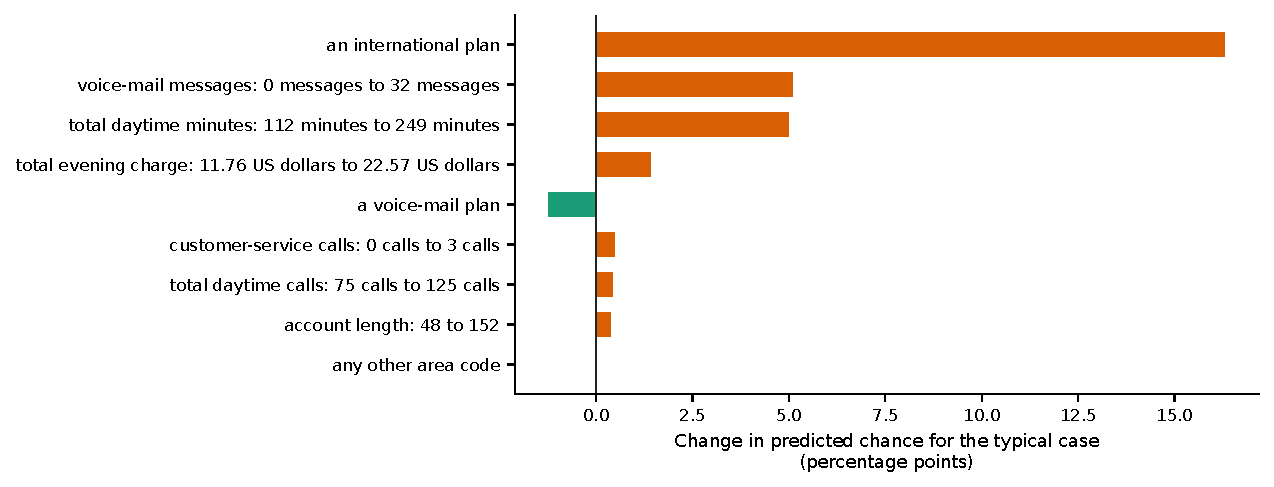
\includegraphics[width=\linewidth,height=0.88\textheight,keepaspectratio]{figures/churn100-s4-c3/ann_88-effects.pdf}
\caption{The whole model: Each input's change in the predicted value for the typical case across the whole model, largest first (orange: raises it, teal: lowers it).}
\label{fig:churn100s4c3:plot-ann88-0}
\end{figure}
\begin{figure}[H]\centering
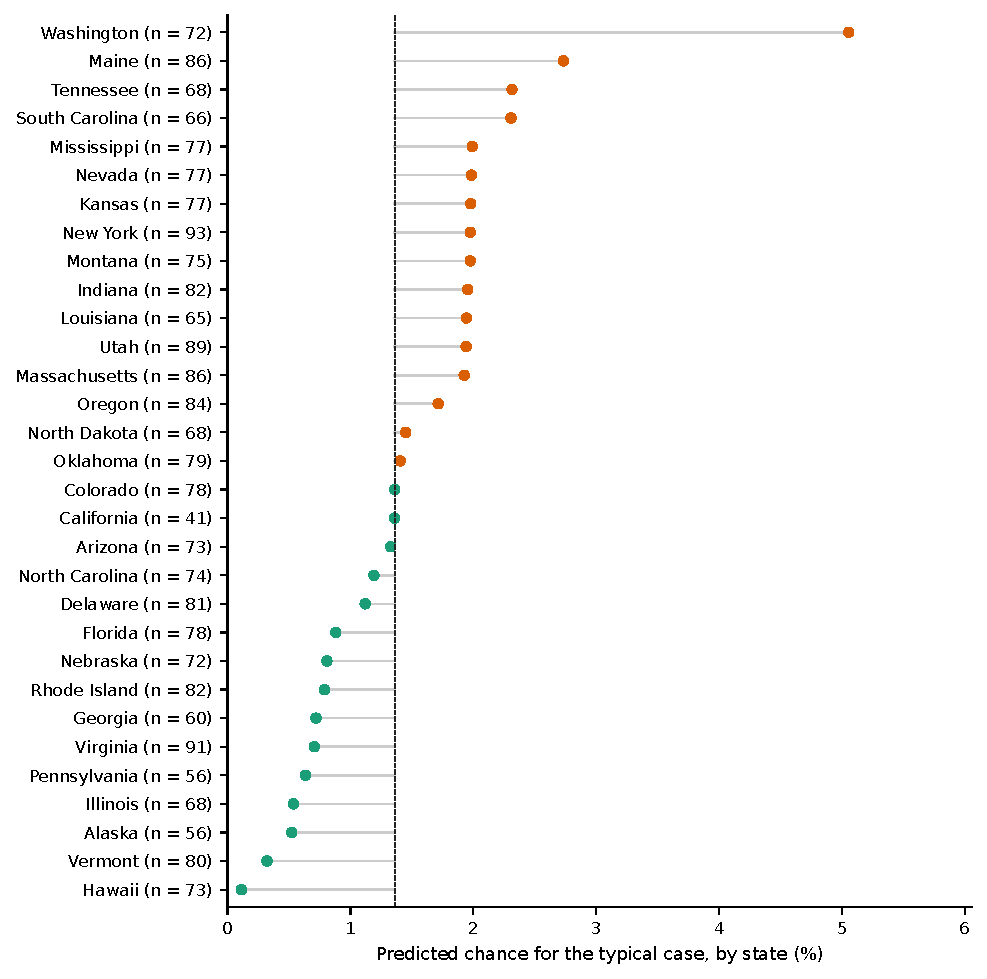
\includegraphics[width=\linewidth,height=0.88\textheight,keepaspectratio]{figures/churn100-s4-c3/ann_88-levels-state.pdf}
\caption{The whole model: Every level of state the model reads: the predicted value for the typical case at that level (dashed: the reference level); n = training customers; grey: few customers or not supported.}
\label{fig:churn100s4c3:plot-ann88-1}
\end{figure}
\par\smallskip\noindent{\small \textbf{Dive deeper:} Fixed-weight inputs (\ref{rd:ann82}); Service calls (\ref{rd:ann87}); Heavy daytime use (\ref{rd:ann85}); State units (\ref{rd:ann86}). Technical detail: \ref{tech:ann88}.\par}
\subsubsection{Fixed-weight inputs}\label{rd:ann82}
\noindent{\footnotesize Part of: The whole model (\ref{rd:ann88}).\par}
\noindent{\small Figure~\ref{fig:churn100s4c3:parts-ann82} shows what feeds this part; Figure~\ref{fig:churn100s4c3:units-ann82} its units and every connection into them (dashed boxes: connections from or to other parts, drawn in their own sections).\par}
\begin{figure}[H]\centering
\resizebox{!}{\ifdim\height>0.5\textheight 0.5\textheight\else\height\fi}{%
\resizebox{\ifdim\width>\linewidth\linewidth\else\width\fi}{!}{%
\begin{tikzpicture}[
  font=\sffamily\scriptsize, >={Stealth[length=1.6mm]},
  inp/.style={draw, rounded corners=1pt, fill=white, inner sep=1.5pt, minimum height=3.2mm, anchor=east},
  abox/.style={draw, thick, rounded corners=2pt, align=center, inner sep=3pt, minimum height=6mm, text width=42mm},
  outp/.style={draw, double, rounded corners=2pt, fill=white, align=center, inner sep=3pt, text width=24mm},
  agg/.style={draw=black!55},
]
\node[inp] (i0) at (0,2.625) {state};
\node[inp] (i1) at (0,1.875) {account length};
\node[inp] (i2) at (0,1.125) {area code};
\node[inp] (i3) at (0,0.375) {international calling plan};
\node[inp] (i4) at (0,-0.375) {voice-mail plan};
\node[inp] (i5) at (0,-1.125) {voice-mail messages};
\node[inp] (i6) at (0,-1.875) {total daytime calls};
\node[inp] (i7) at (0,-2.625) {total evening charge};
\node[outp] (out) at (9.36,0) {Fixed-weight inputs};
\begin{scope}[on background layer]
\draw[->, agg, thin, dashed] (i0.east) -- (out.west);
\draw[->, agg, thin, dashed] (i1.east) -- (out.west);
\draw[->, agg, thin, dashed] (i2.east) -- (out.west);
\draw[->, agg, thin, dashed] (i3.east) -- (out.west);
\draw[->, agg, thin, dashed] (i4.east) -- (out.west);
\draw[->, agg, thin, dashed] (i5.east) -- (out.west);
\draw[->, agg, thin, dashed] (i6.east) -- (out.west);
\draw[->, agg, thin, dashed] (i7.east) -- (out.west);
\end{scope}
\end{tikzpicture}}}%
\caption{Fixed-weight inputs: what feeds it, one level down.}
\label{fig:churn100s4c3:parts-ann82}
\end{figure}
\begin{figure}[H]\centering
\resizebox{\ifdim\width>\linewidth\linewidth\else\width\fi}{!}{%
\definecolor{netup}{HTML}{D95F02}\definecolor{netdown}{HTML}{1B9E77}\definecolor{netmixed}{HTML}{7F7F7F}%
\begin{tikzpicture}[
  font=\sffamily\scriptsize, >={Stealth[length=1.4mm]},
  inp/.style={draw, circle, fill=white, minimum size=3.2mm, inner sep=0pt},
  hid/.style={draw, circle, fill=white, minimum size=5.2mm, inner sep=0.5pt, font=\sffamily\tiny},
  exitbox/.style={draw, thick, rectangle, fill=white, align=center, text width=17mm, minimum height=5mm, inner sep=1.5pt, font=\sffamily\tiny},
  sumbox/.style={draw, thick, dashed, rectangle, fill=white, align=center, text width=17mm, minimum height=5mm, inner sep=1.5pt, font=\sffamily\tiny},
  outp/.style={draw, thick, regular polygon, regular polygon sides=6, fill=white, minimum size=10mm, inner sep=0pt, font=\sffamily\tiny, align=center},
  stub/.style={draw, dashed, rounded corners=2pt, fill=white, align=center, inner sep=2pt, font=\sffamily\tiny, text width=15mm},
  inlab/.style={font=\sffamily\tiny, align=center, text width=15mm, inner sep=1pt, fill=white, fill opacity=0.8, text opacity=1},
  wpos/.style={draw=NavyBlue}, wneg/.style={draw=BrickRed}, wagg/.style={draw=black!45, line width=1.2pt},
  wmix/.style={draw=Plum},
]
\node[exitbox] (nidentityxlin) at (5.85,1.9) {Fixed-weight inputs $\uparrow$};
\node[inp, draw=netmixed, very thick] (ngrpxxstate) at (4.5,0.0) {};
\path (ngrpxxstate.south) node[inlab, anchor=north] (labngrpxxstate) {state (31 of 51 used) $\updownarrow$};
\node[inp, draw=netup, very thick] (ninxxaccountxlength) at (1.8,-1.05) {};
\path (ninxxaccountxlength.south) node[inlab, anchor=north] (labninxxaccountxlength) {account length $\uparrow$};
\node[inp, draw=netup, very thick] (ninxxareaxcodex415) at (3.6,-1.05) {};
\path (ninxxareaxcodex415.south) node[inlab, anchor=north] (labninxxareaxcodex415) {area code 415 $\uparrow$};
\node[inp, draw=netup, very thick] (ninxxinternationalxplan) at (2.7,0.0) {};
\path (ninxxinternationalxplan.south) node[inlab, anchor=north] (labninxxinternationalxplan) {an international plan $\uparrow$};
\node[inp, draw=netup, very thick] (ninxxnumberxvmailxmessages) at (9.9,0.0) {};
\path (ninxxnumberxvmailxmessages.south) node[inlab, anchor=north] (labninxxnumberxvmailxmessages) {voice-mail messages $\uparrow$};
\node[inp, draw=netup, very thick] (ninxxtotalxevexcharge) at (8.1,0.0) {};
\path (ninxxtotalxevexcharge.south) node[inlab, anchor=north] (labninxxtotalxevexcharge) {total evening charge $\uparrow$};
\node[inp, draw=netup, very thick] (ninxxtotalxdayxcalls) at (6.3,0.0) {};
\path (ninxxtotalxdayxcalls.south) node[inlab, anchor=north] (labninxxtotalxdayxcalls) {total daytime calls $\uparrow$};
\node[inp, draw=netdown, very thick] (ninxxvoicexmailxplan) at (0.9,0.0) {};
\path (ninxxvoicexmailxplan.south) node[inlab, anchor=north] (labninxxvoicexmailxplan) {a voice-mail plan $\downarrow$};
\node[stub] (ntoxxthexmodelxoutput) at (5.4,3.45) {to the model output};
\begin{scope}[on background layer]
\node[fit=(nidentityxlin) , inner sep=8pt, rounded corners=5pt, fill=BurntOrange!10, draw=BurntOrange!45] (clu0) {};
\draw[->, wpos, line width=0.29pt] (ninxxaccountxlength) -- (nidentityxlin);
\draw[->, wpos, line width=0.25pt] (ninxxareaxcodex415) -- (nidentityxlin);
\draw[->, wpos, line width=0.53pt] (ninxxinternationalxplan) -- (nidentityxlin);
\draw[->, wpos, line width=0.49pt] (ninxxnumberxvmailxmessages) -- (nidentityxlin);
\draw[->, wpos, line width=0.39pt] (ninxxtotalxevexcharge) -- (nidentityxlin);
\draw[->, wpos, line width=0.29pt] (ninxxtotalxdayxcalls) -- (nidentityxlin);
\draw[->, wneg, line width=0.62pt] (ninxxvoicexmailxplan) -- (nidentityxlin);
\draw[->, wpos, line width=0.60pt] (nidentityxlin) -- (ntoxxthexmodelxoutput);
\draw[->, wmix, line width=0.39pt] (ngrpxxstate) -- node[pos=0.8, sloped, above, font=\sffamily\tiny, inner sep=1pt, fill=white, fill opacity=0.8, text opacity=1] {21 edges, -0.40 to +0.18} (nidentityxlin);
\end{scope}
\node[font=\sffamily\scriptsize\bfseries, text=BurntOrange!55!black, anchor=south west, inner sep=1pt, fill=white, fill opacity=0.85, text opacity=1] at (clu0.north west) {Fixed-weight inputs};
\end{tikzpicture}}%
\caption{Fixed-weight inputs: its units and every connection into them. Blue: positive weight (raises the score); red: negative weight (lowers it); thicker: larger weight. Orange outline and up arrow: raises the final prediction; teal and down arrow: lowers it; grey and double arrow: depends.}
\label{fig:churn100s4c3:units-ann82}
\end{figure}
\paragraph{Hypothesis.} This part adds up most inputs with fixed weights: an international plan, voice-mail messages and the evening charge raise the chance of leaving, steadily for the numbers, and a voice-mail plan lowers it.\,{\scriptsize\textcolor{NavyBlue}{[C055, C056, C059, C063]}}
\paragraph{Evidence.} Through it, an international plan takes a typical customer from about 1\% to about 18\%, and a voice-mail plan lowers the chance to below 1\%.\,{\scriptsize\textcolor{NavyBlue}{[C055, C063]}} More voice-mail messages raise it steadily, from about 1\% at 0 to about 6\% at 32 messages, flattening out near the bottom because the predicted chance cannot go much lower.\,{\scriptsize\textcolor{NavyBlue}{[C056]}} A higher evening charge also raises it steadily, from about 1\% at 11.76 US dollars to about 2\% at 22.57 US dollars, flattening out near the bottom because the predicted chance cannot go much lower.\,{\scriptsize\textcolor{NavyBlue}{[C059]}} Through it, the state moves the chance from about 1\% in West Virginia to about 5\% in Washington and about 4\% in Nevada, and to below 1\% in Rhode Island, Hawaii and Vermont (72 to 82 training customers per state).\,{\scriptsize\textcolor{NavyBlue}{[C057, C058, C061, C062, C064]}} Its formula reproduces the part exactly on all 4000 training customers.\,{\scriptsize\textcolor{NavyBlue}{[C083]}}
\par\noindent{\small Evidence plots: Figure~\ref{fig:churn100s4c3:plot-ann82-0}, Figure~\ref{fig:churn100s4c3:plot-ann82-1}, Figure~\ref{fig:churn100s4c3:plot-ann82-2}, Figure~\ref{fig:churn100s4c3:plot-ann82-3}.\par}
\begin{figure}[H]\centering
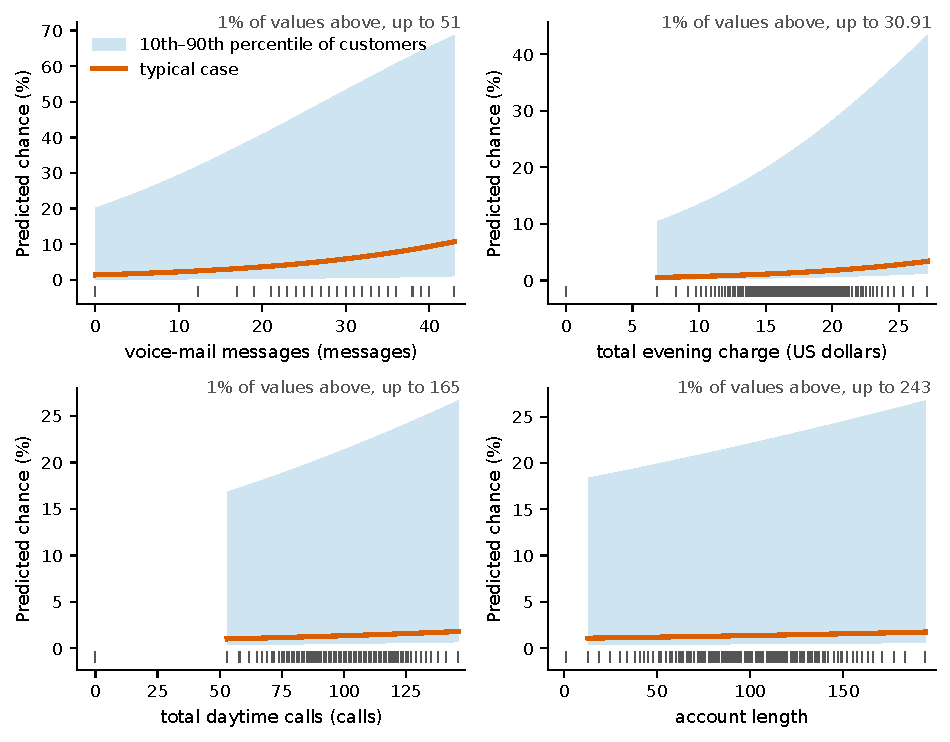
\includegraphics[width=\linewidth,height=0.88\textheight,keepaspectratio]{figures/churn100-s4-c3/ann_82-response.pdf}
\caption{Fixed-weight inputs: Response curves through this part: the typical case (bold), the 10th to 90th percentile of individual customers (band), the fold or step point (dashed) with its spread across them (grey), and the observed values (ticks).}
\label{fig:churn100s4c3:plot-ann82-0}
\end{figure}
\begin{figure}[H]\centering
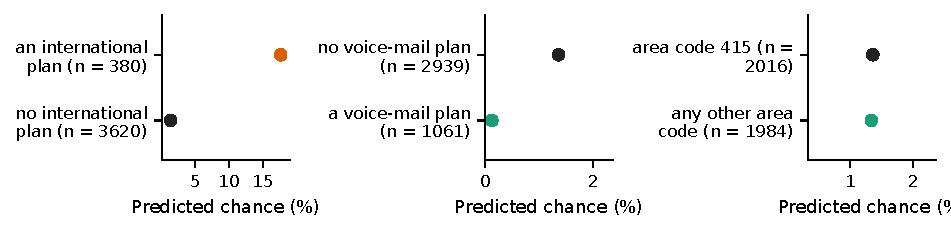
\includegraphics[width=\linewidth,height=0.88\textheight,keepaspectratio]{figures/churn100-s4-c3/ann_82-categories-small.pdf}
\caption{Fixed-weight inputs: The predicted value for the typical case at each level, through this part (n = training customers; grey: fewer than 20).}
\label{fig:churn100s4c3:plot-ann82-1}
\end{figure}
\begin{figure}[H]\centering
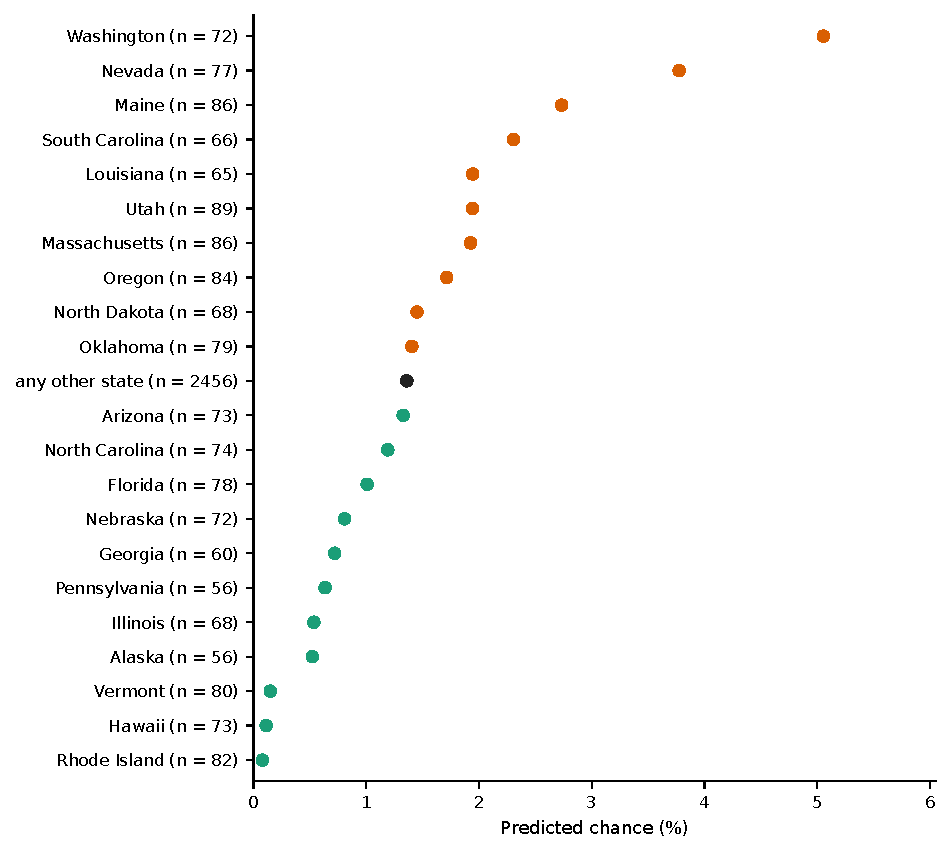
\includegraphics[width=\linewidth,height=0.88\textheight,keepaspectratio]{figures/churn100-s4-c3/ann_82-categories-C057.pdf}
\caption{Fixed-weight inputs: The predicted value for the typical case at each level, through this part (n = training customers; grey: fewer than 20).}
\label{fig:churn100s4c3:plot-ann82-2}
\end{figure}
\begin{figure}[H]\centering
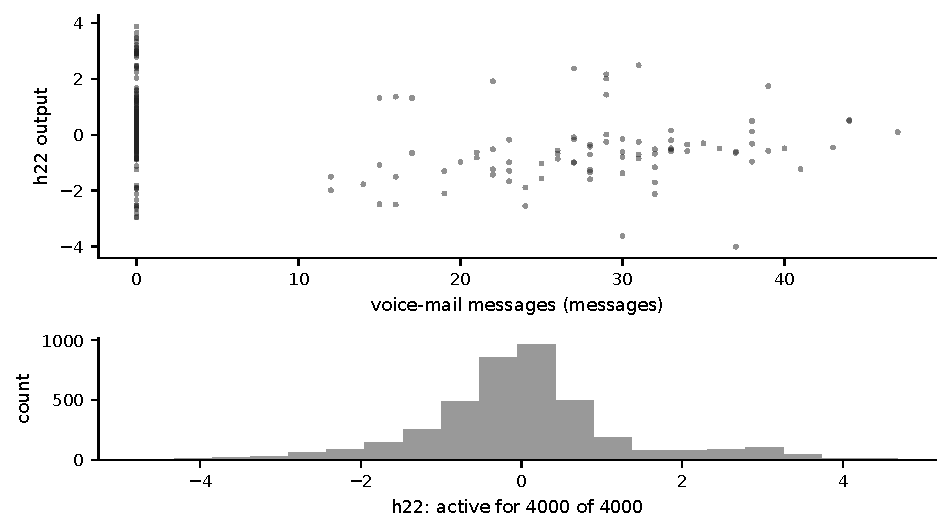
\includegraphics[width=\linewidth,height=0.88\textheight,keepaspectratio]{figures/churn100-s4-c3/ann_82-units.pdf}
\caption{Fixed-weight inputs: This part's hidden units: each unit's output against its main numeric input (top) and how often it is active (bottom).}
\label{fig:churn100s4c3:plot-ann82-3}
\end{figure}
\par\smallskip\noindent{\small Technical detail: \ref{tech:ann82}.\par}
\subsubsection{Service calls}\label{rd:ann87}
\noindent{\footnotesize Part of: The whole model (\ref{rd:ann88}).\par}
\noindent{\small Figure~\ref{fig:churn100s4c3:parts-ann87} shows what feeds this part; Figure~\ref{fig:churn100s4c3:units-ann87} its units and every connection into them (dashed boxes: connections from or to other parts, drawn in their own sections).\par}
\begin{figure}[H]\centering
\resizebox{!}{\ifdim\height>0.5\textheight 0.5\textheight\else\height\fi}{%
\resizebox{\ifdim\width>\linewidth\linewidth\else\width\fi}{!}{%
\begin{tikzpicture}[
  font=\sffamily\scriptsize, >={Stealth[length=1.6mm]},
  inp/.style={draw, rounded corners=1pt, fill=white, inner sep=1.5pt, minimum height=3.2mm, anchor=east},
  abox/.style={draw, thick, rounded corners=2pt, align=center, inner sep=3pt, minimum height=6mm, text width=42mm},
  outp/.style={draw, double, rounded corners=2pt, fill=white, align=center, inner sep=3pt, text width=24mm},
  agg/.style={draw=black!55},
]
\node[inp] (i0) at (0,0.375) {state};
\node[inp] (i1) at (0,-0.375) {customer-service calls};
\node[abox, fill=RoyalBlue!18, draw=RoyalBlue!80!black] (b0) at (5.28,0.5) {\textbf{Early rise in calls}};
\node[abox, fill=BurntOrange!18, draw=BurntOrange!80!black] (b1) at (5.28,-0.5) {\textbf{Late rise in calls}};
\node[outp] (out) at (9.36,0) {Service calls};
\begin{scope}[on background layer]
\draw[->, agg, thin] (i0.east) -- (b0.west);
\draw[->, agg, thin] (i1.east) -- (b0.west);
\draw[->, agg] (b0.east) -- (out.west);
\draw[->, agg, thin] (i0.east) -- (b1.west);
\draw[->, agg, thin] (i1.east) -- (b1.west);
\draw[->, agg] (b1.east) -- (out.west);
\end{scope}
\end{tikzpicture}}}%
\caption{Service calls: what feeds it, one level down.}
\label{fig:churn100s4c3:parts-ann87}
\end{figure}
\begin{figure}[H]\centering
\resizebox{\ifdim\width>\linewidth\linewidth\else\width\fi}{!}{%
\definecolor{netup}{HTML}{D95F02}\definecolor{netdown}{HTML}{1B9E77}\definecolor{netmixed}{HTML}{7F7F7F}%
\begin{tikzpicture}[
  font=\sffamily\scriptsize, >={Stealth[length=1.4mm]},
  inp/.style={draw, circle, fill=white, minimum size=3.2mm, inner sep=0pt},
  hid/.style={draw, circle, fill=white, minimum size=5.2mm, inner sep=0.5pt, font=\sffamily\tiny},
  exitbox/.style={draw, thick, rectangle, fill=white, align=center, text width=17mm, minimum height=5mm, inner sep=1.5pt, font=\sffamily\tiny},
  sumbox/.style={draw, thick, dashed, rectangle, fill=white, align=center, text width=17mm, minimum height=5mm, inner sep=1.5pt, font=\sffamily\tiny},
  outp/.style={draw, thick, regular polygon, regular polygon sides=6, fill=white, minimum size=10mm, inner sep=0pt, font=\sffamily\tiny, align=center},
  stub/.style={draw, dashed, rounded corners=2pt, fill=white, align=center, inner sep=2pt, font=\sffamily\tiny, text width=15mm},
  inlab/.style={font=\sffamily\tiny, align=center, text width=15mm, inner sep=1pt, fill=white, fill opacity=0.8, text opacity=1},
  wpos/.style={draw=NavyBlue}, wneg/.style={draw=BrickRed}, wagg/.style={draw=black!45, line width=1.2pt},
  wmix/.style={draw=Plum},
]
\node[exitbox] (nidentityxsvc) at (1.8,1.9) {Service calls $\uparrow$};
\node[stub] (nfromxxLatexrisexinxcalls) at (2.7,0.0) {from Late rise in calls};
\node[stub] (nfromxxEarlyxrisexinxcalls) at (0.9,0.0) {from Early rise in calls};
\node[stub] (ntoxxthexmodelxoutput) at (1.8,3.45) {to the model output};
\begin{scope}[on background layer]
\node[fit=(nidentityxsvc) , inner sep=8pt, rounded corners=5pt, fill=ForestGreen!10, draw=ForestGreen!45] (clu0) {};
\draw[->, wpos, line width=0.85pt] (nfromxxLatexrisexinxcalls) -- (nidentityxsvc);
\draw[->, wpos, line width=0.91pt] (nfromxxEarlyxrisexinxcalls) -- (nidentityxsvc);
\draw[->, wpos, line width=0.86pt] (nfromxxEarlyxrisexinxcalls) -- (nidentityxsvc);
\draw[->, wpos, line width=0.60pt] (nidentityxsvc) -- (ntoxxthexmodelxoutput);
\end{scope}
\node[font=\sffamily\scriptsize\bfseries, text=ForestGreen!55!black, anchor=south west, inner sep=1pt, fill=white, fill opacity=0.85, text opacity=1] at (clu0.north west) {Service calls};
\end{tikzpicture}}%
\caption{Service calls: its units and every connection into them. Blue: positive weight (raises the score); red: negative weight (lowers it); thicker: larger weight. Orange outline and up arrow: raises the final prediction; teal and down arrow: lowers it; grey and double arrow: depends.}
\label{fig:churn100s4c3:units-ann87}
\end{figure}
\paragraph{Hypothesis.} This part raises the chance of leaving with calls to customer service, slowly at first, then faster from about 3 calls upwards; it adds up two parts.\,{\scriptsize\textcolor{NavyBlue}{[C090, C089]}}
\paragraph{Evidence.} It is made of two parts that are added: an early rise and a late rise in calls to customer service.\,{\scriptsize\textcolor{NavyBlue}{[C090]}} From about 3 calls upwards it adds to the chance slowly at first, then faster: for a typical such customer, 4 calls take it from about 1\% to about 10\%, flattening out near the bottom because the predicted chance cannot go much lower.\,{\scriptsize\textcolor{NavyBlue}{[C089]}} Up to 3 calls the chance rises slowly at first, then faster, from about 1\% to about 2\% for a typical customer, flattening out near the bottom because the predicted chance cannot go much lower.\,{\scriptsize\textcolor{NavyBlue}{[C084]}} That early rise happens only outside Nebraska, California and Colorado: in Nebraska the chance stays at about 1\% from 0 to 3 calls, against a rise from about 1\% to about 2\% elsewhere, slowly at first, then faster, flattening out near the bottom because the predicted chance cannot go much lower.\,{\scriptsize\textcolor{NavyBlue}{[C088]}}
\par\noindent{\small Evidence plots: Figure~\ref{fig:churn100s4c3:plot-ann87-0}, Figure~\ref{fig:churn100s4c3:plot-ann87-1}, Figure~\ref{fig:churn100s4c3:plot-ann87-2}, Figure~\ref{fig:churn100s4c3:plot-ann87-3}, Figure~\ref{fig:churn100s4c3:plot-ann87-4}.\par}
\par\noindent{\small Figure~\ref{fig:churn100s4c3:plot-ann87-3} shows this part's own output, unit h23: it switches on at about 2.827 calls of customer-service calls, and is zero below.\par}
\begin{figure}[H]\centering
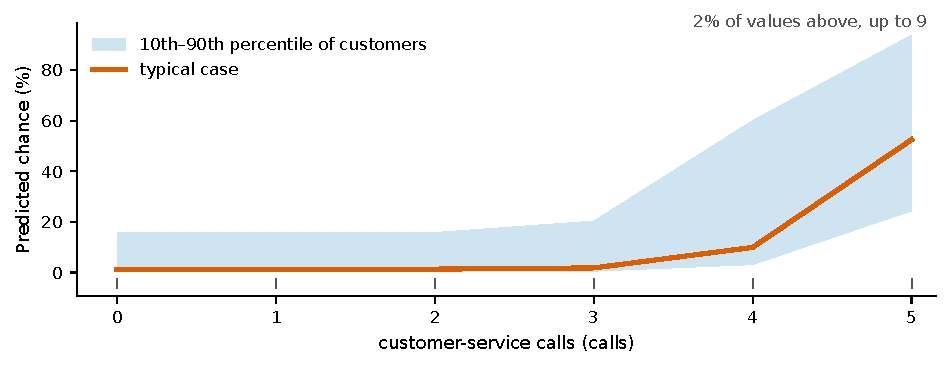
\includegraphics[width=\linewidth,height=0.88\textheight,keepaspectratio]{figures/churn100-s4-c3/ann_87-response.pdf}
\caption{Service calls: Response curves through this part: the typical case (bold), the 10th to 90th percentile of individual customers (band), the fold or step point (dashed) with its spread across them (grey), and the observed values (ticks).}
\label{fig:churn100s4c3:plot-ann87-0}
\end{figure}
\begin{figure}[H]\centering
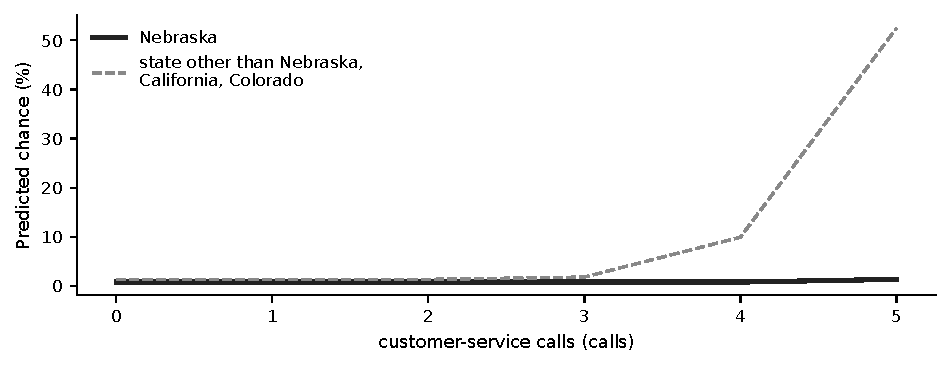
\includegraphics[width=\linewidth,height=0.88\textheight,keepaspectratio]{figures/churn100-s4-c3/ann_87-interaction.pdf}
\caption{Service calls: How the effect differs between groups: one curve per group, for the typical case of each group.}
\label{fig:churn100s4c3:plot-ann87-1}
\end{figure}
\begin{figure}[H]\centering
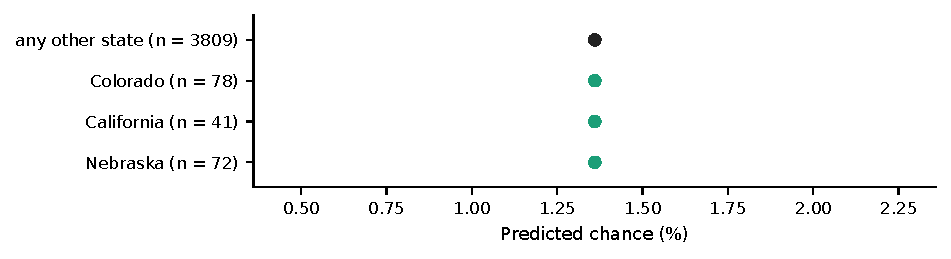
\includegraphics[width=\linewidth,height=0.88\textheight,keepaspectratio]{figures/churn100-s4-c3/ann_87-categories-small.pdf}
\caption{Service calls: The predicted value for the typical case at each level, through this part (n = training customers; grey: fewer than 20).}
\label{fig:churn100s4c3:plot-ann87-2}
\end{figure}
\begin{figure}[H]\centering
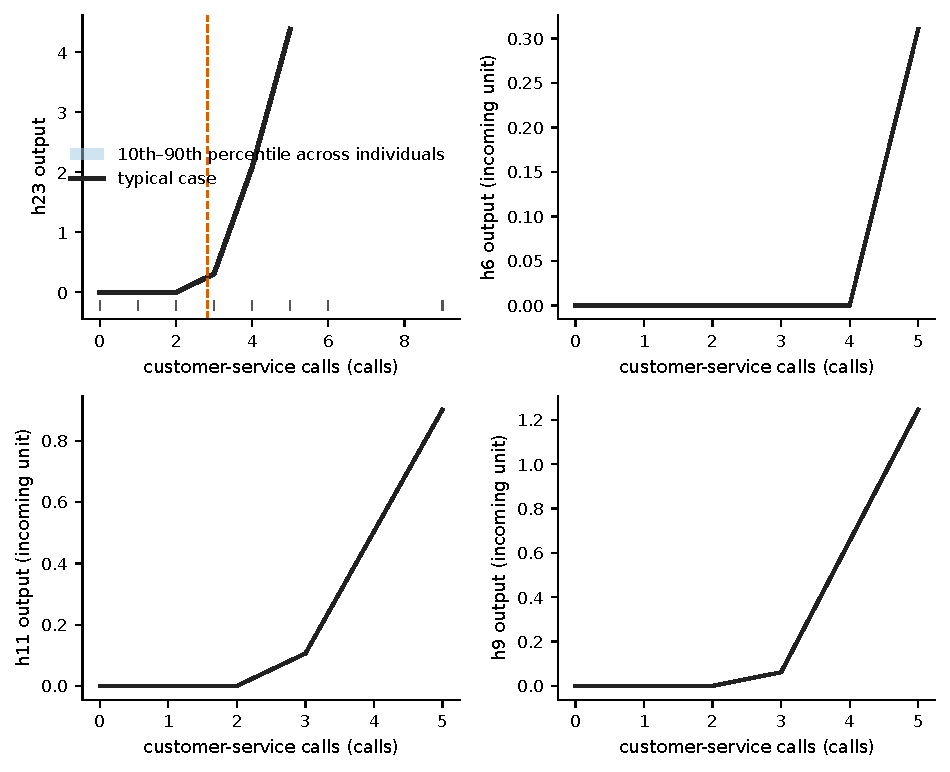
\includegraphics[width=\linewidth,height=0.88\textheight,keepaspectratio]{figures/churn100-s4-c3/ann_87-partial-identity_svc.pdf}
\caption{Service calls: This part's own output, unit h23 (combines 3 non-linear units), on its own scale (its activation), with every other input at the typical case; it is active for 831 of 4000. Bold: the typical case; band: 10th to 90th percentile across individuals; dashed: where it switches on; ticks: the data.}
\label{fig:churn100s4c3:plot-ann87-3}
\end{figure}
\begin{figure}[H]\centering
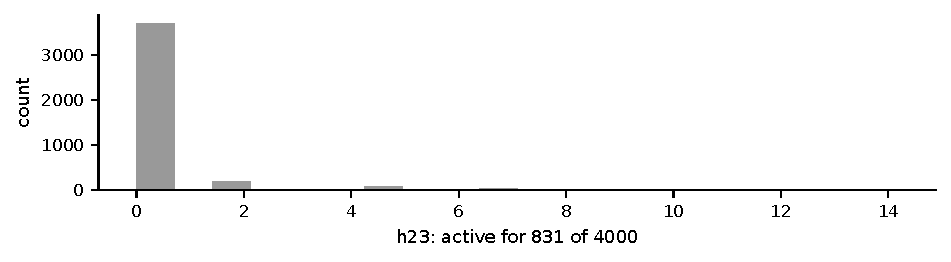
\includegraphics[width=\linewidth,height=0.88\textheight,keepaspectratio]{figures/churn100-s4-c3/ann_87-units.pdf}
\caption{Service calls: This part's hidden units: each unit's output against its main numeric input (top) and how often it is active (bottom).}
\label{fig:churn100s4c3:plot-ann87-4}
\end{figure}
\par\smallskip\noindent{\small \textbf{Dive deeper:} Early rise in calls (\ref{rd:ann84}); Late rise in calls (\ref{rd:ann83}). Technical detail: \ref{tech:ann87}.\par}
\subsubsection{Early rise in calls}\label{rd:ann84}
\noindent{\footnotesize Part of: Service calls (\ref{rd:ann87}).\par}
\noindent{\small Figure~\ref{fig:churn100s4c3:parts-ann84} shows what feeds this part; Figure~\ref{fig:churn100s4c3:units-ann84} its units and every connection into them (dashed boxes: connections from or to other parts, drawn in their own sections).\par}
\begin{figure}[H]\centering
\resizebox{!}{\ifdim\height>0.5\textheight 0.5\textheight\else\height\fi}{%
\resizebox{\ifdim\width>\linewidth\linewidth\else\width\fi}{!}{%
\begin{tikzpicture}[
  font=\sffamily\scriptsize, >={Stealth[length=1.6mm]},
  inp/.style={draw, rounded corners=1pt, fill=white, inner sep=1.5pt, minimum height=3.2mm, anchor=east},
  abox/.style={draw, thick, rounded corners=2pt, align=center, inner sep=3pt, minimum height=6mm, text width=42mm},
  outp/.style={draw, double, rounded corners=2pt, fill=white, align=center, inner sep=3pt, text width=24mm},
  agg/.style={draw=black!55},
]
\node[inp] (i0) at (0,0.375) {state};
\node[inp] (i1) at (0,-0.375) {customer-service calls};
\node[outp] (out) at (9.36,0) {Early rise in calls};
\begin{scope}[on background layer]
\draw[->, agg, thin, dashed] (i0.east) -- (out.west);
\draw[->, agg, thin, dashed] (i1.east) -- (out.west);
\end{scope}
\end{tikzpicture}}}%
\caption{Early rise in calls: what feeds it, one level down.}
\label{fig:churn100s4c3:parts-ann84}
\end{figure}
\begin{figure}[H]\centering
\resizebox{\ifdim\width>\linewidth\linewidth\else\width\fi}{!}{%
\definecolor{netup}{HTML}{D95F02}\definecolor{netdown}{HTML}{1B9E77}\definecolor{netmixed}{HTML}{7F7F7F}%
\begin{tikzpicture}[
  font=\sffamily\scriptsize, >={Stealth[length=1.4mm]},
  inp/.style={draw, circle, fill=white, minimum size=3.2mm, inner sep=0pt},
  hid/.style={draw, circle, fill=white, minimum size=5.2mm, inner sep=0.5pt, font=\sffamily\tiny},
  exitbox/.style={draw, thick, rectangle, fill=white, align=center, text width=17mm, minimum height=5mm, inner sep=1.5pt, font=\sffamily\tiny},
  sumbox/.style={draw, thick, dashed, rectangle, fill=white, align=center, text width=17mm, minimum height=5mm, inner sep=1.5pt, font=\sffamily\tiny},
  outp/.style={draw, thick, regular polygon, regular polygon sides=6, fill=white, minimum size=10mm, inner sep=0pt, font=\sffamily\tiny, align=center},
  stub/.style={draw, dashed, rounded corners=2pt, fill=white, align=center, inner sep=2pt, font=\sffamily\tiny, text width=15mm},
  inlab/.style={font=\sffamily\tiny, align=center, text width=15mm, inner sep=1pt, fill=white, fill opacity=0.8, text opacity=1},
  wpos/.style={draw=NavyBlue}, wneg/.style={draw=BrickRed}, wagg/.style={draw=black!45, line width=1.2pt},
  wmix/.style={draw=Plum},
]
\node[hid] (n6713) at (1.9,3.25) {h9};
\node[hid] (n9436) at (1.9,1.9) {h11};
\node[inp, draw=netup, very thick] (ninxxnumberxcustomerxservicexcalls) at (1.0,0.0) {};
\path (ninxxnumberxcustomerxservicexcalls.south) node[inlab, anchor=north] (labninxxnumberxcustomerxservicexcalls) {customer-service calls $\uparrow$};
\node[inp, draw=netmixed, very thick] (ngrpxxstate) at (2.8,0.0) {};
\path (ngrpxxstate.south) node[inlab, anchor=north] (labngrpxxstate) {state (31 of 51 used) $\updownarrow$};
\node[stub] (ntoxxServicexcalls) at (1.9,4.8) {to Service calls};
\begin{scope}[on background layer]
\node[fit=(n6713) (n9436) , inner sep=8pt, rounded corners=5pt, fill=ForestGreen!10, draw=ForestGreen!45] (clu0) {};
\draw[->, wpos, line width=0.77pt] (n9436) -- (n6713);
\draw[->, wpos, line width=0.43pt] (ninxxnumberxcustomerxservicexcalls) -- (n9436);
\draw[->, wpos, line width=0.91pt] (n9436) -- (ntoxxServicexcalls);
\draw[->, wpos, line width=0.86pt] (n6713) -- (ntoxxServicexcalls);
\draw[->, wneg, line width=0.64pt] (ngrpxxstate) -- node[pos=0.8, sloped, above, font=\sffamily\tiny, inner sep=1pt, fill=white, fill opacity=0.8, text opacity=1] {-1.12} (n9436);
\end{scope}
\node[font=\sffamily\scriptsize\bfseries, text=ForestGreen!55!black, anchor=south west, inner sep=1pt, fill=white, fill opacity=0.85, text opacity=1] at (clu0.north west) {Early rise in calls};
\end{tikzpicture}}%
\caption{Early rise in calls: its units and every connection into them. Blue: positive weight (raises the score); red: negative weight (lowers it); thicker: larger weight. Orange outline and up arrow: raises the final prediction; teal and down arrow: lowers it; grey and double arrow: depends.}
\label{fig:churn100s4c3:units-ann84}
\end{figure}
\paragraph{Hypothesis.} This part raises the chance of leaving from about 3 customer-service calls upwards, in an uneven way.\,{\scriptsize\textcolor{NavyBlue}{[C094]}}
\paragraph{Evidence.} It acts on 830 of 4000 training customers, 213 of whom left; for the typical customer it acts on, the chance is about 1\% without it and about 2\% with it.\,{\scriptsize\textcolor{NavyBlue}{[C095]}} Through it, calls add to the chance only from about 3 calls upwards, in an uneven way: for a typical such customer, 4 calls take it from about 1\% to about 10\%, flattening out near the bottom because the predicted chance cannot go much lower.\,{\scriptsize\textcolor{NavyBlue}{[C094]}} Up to 3 calls it raises the chance slowly at first, then faster, but only outside Nebraska: there from about 1\% to about 2\%, while in Nebraska it stays at about 1\%, flattening out near the bottom because the predicted chance cannot go much lower.\,{\scriptsize\textcolor{NavyBlue}{[C093]}} Its formula reproduces the part exactly on all 4000 training customers.\,{\scriptsize\textcolor{NavyBlue}{[C096]}}
\par\noindent{\small Evidence plots: Figure~\ref{fig:churn100s4c3:plot-ann84-0}, Figure~\ref{fig:churn100s4c3:plot-ann84-1}, Figure~\ref{fig:churn100s4c3:plot-ann84-2}, Figure~\ref{fig:churn100s4c3:plot-ann84-3}, Figure~\ref{fig:churn100s4c3:plot-ann84-4}, Figure~\ref{fig:churn100s4c3:plot-ann84-5}.\par}
\par\noindent{\small Figure~\ref{fig:churn100s4c3:plot-ann84-3} shows this part's own output, unit h11: it switches on at about 2.734 calls of customer-service calls, and is zero below.\par}
\par\noindent{\small Figure~\ref{fig:churn100s4c3:plot-ann84-4} shows this part's own output, unit h9: it switches on at about 2.896 calls of customer-service calls, and is zero below.\par}
\begin{figure}[H]\centering
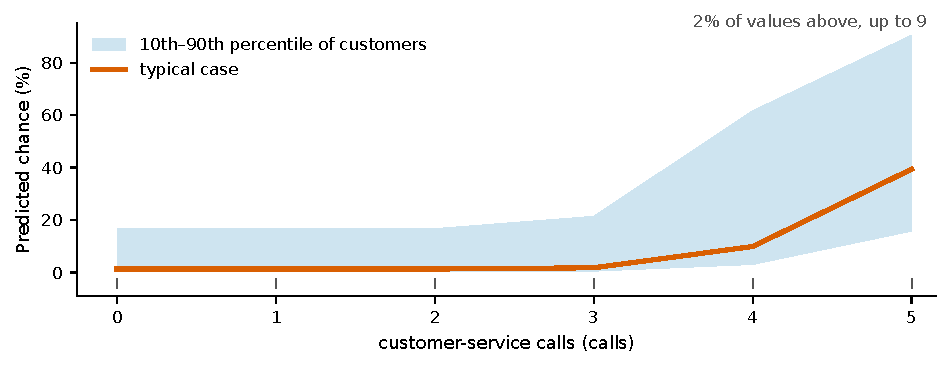
\includegraphics[width=\linewidth,height=0.88\textheight,keepaspectratio]{figures/churn100-s4-c3/ann_84-response.pdf}
\caption{Early rise in calls: Response curves through this part: the typical case (bold), the 10th to 90th percentile of individual customers (band), the fold or step point (dashed) with its spread across them (grey), and the observed values (ticks).}
\label{fig:churn100s4c3:plot-ann84-0}
\end{figure}
\begin{figure}[H]\centering
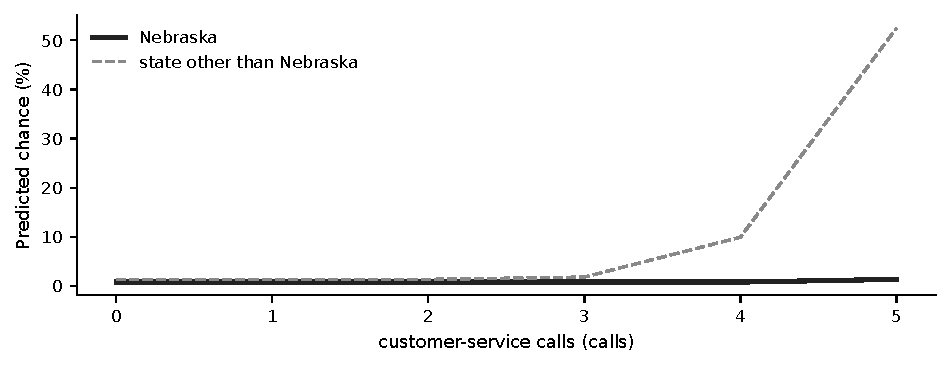
\includegraphics[width=\linewidth,height=0.88\textheight,keepaspectratio]{figures/churn100-s4-c3/ann_84-interaction.pdf}
\caption{Early rise in calls: How the effect differs between groups: one curve per group, for the typical case of each group.}
\label{fig:churn100s4c3:plot-ann84-1}
\end{figure}
\begin{figure}[H]\centering
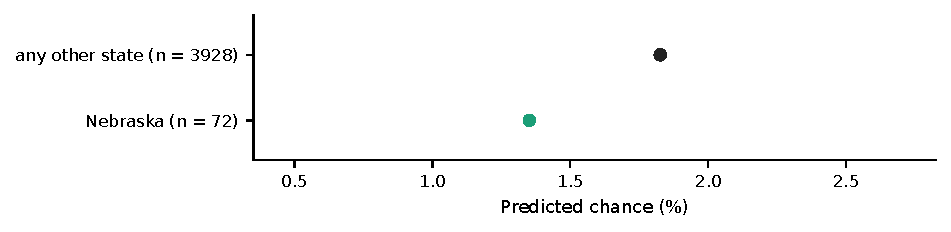
\includegraphics[width=\linewidth,height=0.88\textheight,keepaspectratio]{figures/churn100-s4-c3/ann_84-categories-small.pdf}
\caption{Early rise in calls: The predicted value for the typical case at each level, through this part (n = training customers; grey: fewer than 20).}
\label{fig:churn100s4c3:plot-ann84-2}
\end{figure}
\begin{figure}[H]\centering
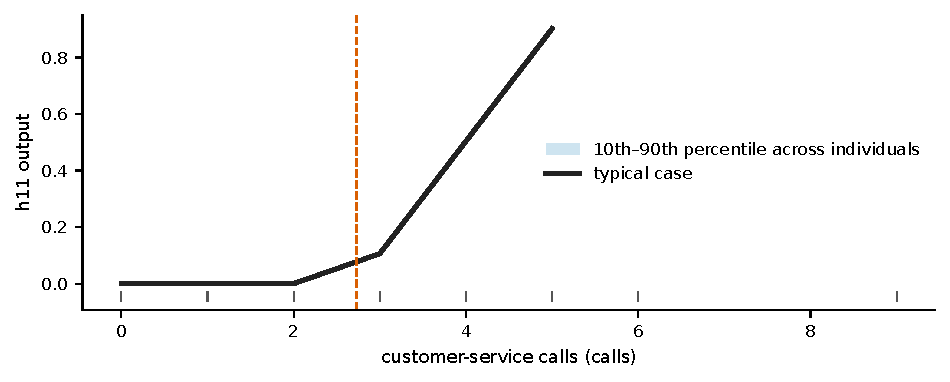
\includegraphics[width=\linewidth,height=0.88\textheight,keepaspectratio]{figures/churn100-s4-c3/ann_84-partial-9436.pdf}
\caption{Early rise in calls: This part's own output, unit h11 (the output of 'Early rise in calls'), on its own scale (its activation), with every other input at the typical case; it is active for 830 of 4000. Bold: the typical case; band: 10th to 90th percentile across individuals; dashed: where it switches on; ticks: the data.}
\label{fig:churn100s4c3:plot-ann84-3}
\end{figure}
\begin{figure}[H]\centering
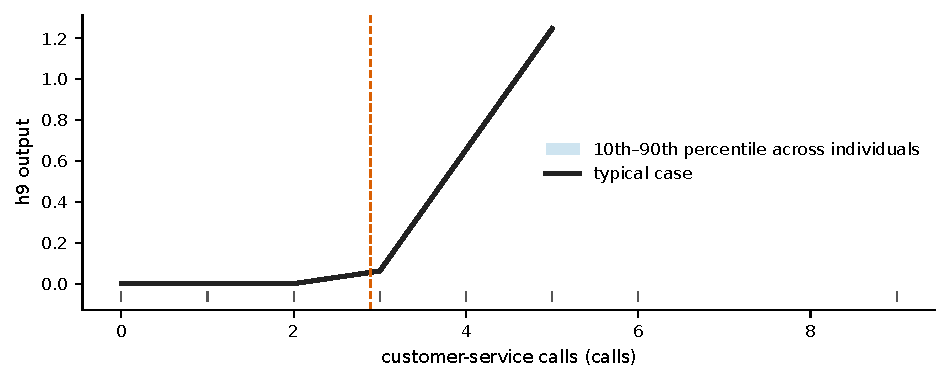
\includegraphics[width=\linewidth,height=0.88\textheight,keepaspectratio]{figures/churn100-s4-c3/ann_84-partial-6713.pdf}
\caption{Early rise in calls: This part's own output, unit h9 (the output of 'Early rise in calls'), on its own scale (its activation), with every other input at the typical case; it is active for 830 of 4000. Bold: the typical case; band: 10th to 90th percentile across individuals; dashed: where it switches on; ticks: the data.}
\label{fig:churn100s4c3:plot-ann84-4}
\end{figure}
\begin{figure}[H]\centering
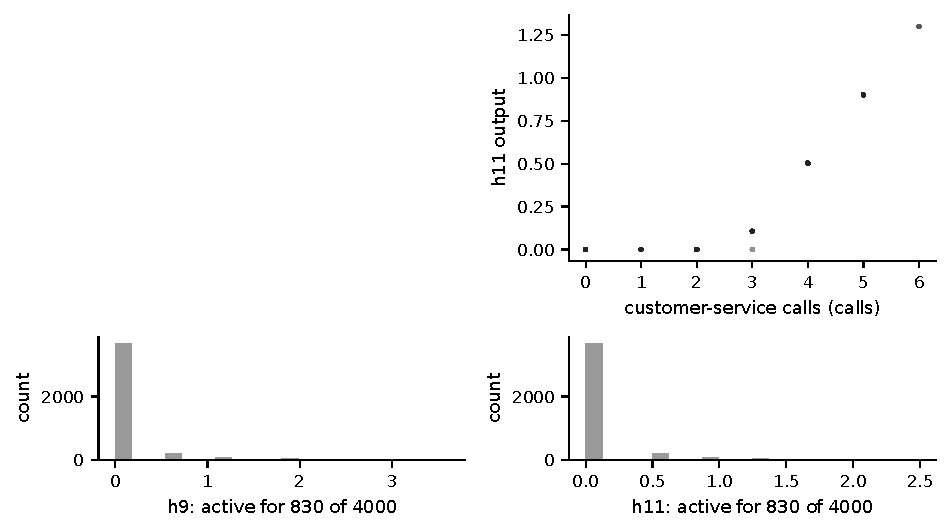
\includegraphics[width=\linewidth,height=0.88\textheight,keepaspectratio]{figures/churn100-s4-c3/ann_84-units.pdf}
\caption{Early rise in calls: This part's hidden units: each unit's output against its main numeric input (top) and how often it is active (bottom).}
\label{fig:churn100s4c3:plot-ann84-5}
\end{figure}
\par\smallskip\noindent{\small Technical detail: \ref{tech:ann84}.\par}
\subsubsection{Late rise in calls}\label{rd:ann83}
\noindent{\footnotesize Part of: Service calls (\ref{rd:ann87}).\par}
\noindent{\small Figure~\ref{fig:churn100s4c3:parts-ann83} shows what feeds this part; Figure~\ref{fig:churn100s4c3:units-ann83} its units and every connection into them (dashed boxes: connections from or to other parts, drawn in their own sections).\par}
\begin{figure}[H]\centering
\resizebox{!}{\ifdim\height>0.5\textheight 0.5\textheight\else\height\fi}{%
\resizebox{\ifdim\width>\linewidth\linewidth\else\width\fi}{!}{%
\begin{tikzpicture}[
  font=\sffamily\scriptsize, >={Stealth[length=1.6mm]},
  inp/.style={draw, rounded corners=1pt, fill=white, inner sep=1.5pt, minimum height=3.2mm, anchor=east},
  abox/.style={draw, thick, rounded corners=2pt, align=center, inner sep=3pt, minimum height=6mm, text width=42mm},
  outp/.style={draw, double, rounded corners=2pt, fill=white, align=center, inner sep=3pt, text width=24mm},
  agg/.style={draw=black!55},
]
\node[inp] (i0) at (0,0.375) {state};
\node[inp] (i1) at (0,-0.375) {customer-service calls};
\node[outp] (out) at (9.36,0) {Late rise in calls};
\begin{scope}[on background layer]
\draw[->, agg, thin, dashed] (i0.east) -- (out.west);
\draw[->, agg, thin, dashed] (i1.east) -- (out.west);
\end{scope}
\end{tikzpicture}}}%
\caption{Late rise in calls: what feeds it, one level down.}
\label{fig:churn100s4c3:parts-ann83}
\end{figure}
\begin{figure}[H]\centering
\resizebox{\ifdim\width>\linewidth\linewidth\else\width\fi}{!}{%
\definecolor{netup}{HTML}{D95F02}\definecolor{netdown}{HTML}{1B9E77}\definecolor{netmixed}{HTML}{7F7F7F}%
\begin{tikzpicture}[
  font=\sffamily\scriptsize, >={Stealth[length=1.4mm]},
  inp/.style={draw, circle, fill=white, minimum size=3.2mm, inner sep=0pt},
  hid/.style={draw, circle, fill=white, minimum size=5.2mm, inner sep=0.5pt, font=\sffamily\tiny},
  exitbox/.style={draw, thick, rectangle, fill=white, align=center, text width=17mm, minimum height=5mm, inner sep=1.5pt, font=\sffamily\tiny},
  sumbox/.style={draw, thick, dashed, rectangle, fill=white, align=center, text width=17mm, minimum height=5mm, inner sep=1.5pt, font=\sffamily\tiny},
  outp/.style={draw, thick, regular polygon, regular polygon sides=6, fill=white, minimum size=10mm, inner sep=0pt, font=\sffamily\tiny, align=center},
  stub/.style={draw, dashed, rounded corners=2pt, fill=white, align=center, inner sep=2pt, font=\sffamily\tiny, text width=15mm},
  inlab/.style={font=\sffamily\tiny, align=center, text width=15mm, inner sep=1pt, fill=white, fill opacity=0.8, text opacity=1},
  wpos/.style={draw=NavyBlue}, wneg/.style={draw=BrickRed}, wagg/.style={draw=black!45, line width=1.2pt},
  wmix/.style={draw=Plum},
]
\node[exitbox] (n5268) at (1.8,3.25) {Late rise in calls $\uparrow$};
\node[hid] (n12374) at (1.05,1.9) {h15};
\node[hid] (n349) at (2.55,1.9) {h1};
\node[inp, draw=netmixed, very thick] (ngrpxxstate) at (2.7,0.0) {};
\path (ngrpxxstate.south) node[inlab, anchor=north] (labngrpxxstate) {state (31 of 51 used) $\updownarrow$};
\node[inp, draw=netup, very thick] (ninxxnumberxcustomerxservicexcalls) at (0.9,0.0) {};
\path (ninxxnumberxcustomerxservicexcalls.south) node[inlab, anchor=north] (labninxxnumberxcustomerxservicexcalls) {customer-service calls $\uparrow$};
\node[stub] (ntoxxServicexcalls) at (1.8,4.8) {to Service calls};
\begin{scope}[on background layer]
\node[fit=(n5268) (n12374) (n349) , inner sep=8pt, rounded corners=5pt, fill=ForestGreen!10, draw=ForestGreen!45] (clu0) {};
\draw[->, wneg, line width=0.74pt] (n349) -- (n5268);
\draw[->, wpos, line width=0.34pt] (n12374) -- (n5268);
\draw[->, wpos, line width=0.36pt] (ninxxnumberxcustomerxservicexcalls) -- (n5268);
\draw[->, wpos, line width=0.51pt] (ninxxnumberxcustomerxservicexcalls) -- (n12374);
\draw[->, wpos, line width=0.85pt] (n5268) -- (ntoxxServicexcalls);
\draw[->, wmix, line width=0.90pt] (ngrpxxstate) -- node[pos=0.8, sloped, above, font=\sffamily\tiny, inner sep=1pt, fill=white, fill opacity=0.8, text opacity=1] {2 edges, -1.86 to +0.41} (n349);
\end{scope}
\node[font=\sffamily\scriptsize\bfseries, text=ForestGreen!55!black, anchor=south west, inner sep=1pt, fill=white, fill opacity=0.85, text opacity=1] at (clu0.north west) {Late rise in calls};
\end{tikzpicture}}%
\caption{Late rise in calls: its units and every connection into them. Blue: positive weight (raises the score); red: negative weight (lowers it); thicker: larger weight. Orange outline and up arrow: raises the final prediction; teal and down arrow: lowers it; grey and double arrow: depends.}
\label{fig:churn100s4c3:units-ann83}
\end{figure}
\paragraph{Hypothesis.} This part raises the chance of leaving for a small group of customers, more in Colorado and less in California.\,{\scriptsize\textcolor{NavyBlue}{[C122, C117, C118]}}
\paragraph{Evidence.} It acts on 134 of 4000 training customers, 74 of whom left; for the typical customer it acts on, the chance is about 39\% without it and about 75\% with it.\,{\scriptsize\textcolor{NavyBlue}{[C122]}} For the typical customer it acts on, the chance through it is about 75\% in Colorado and about 39\% in California, against about 52\% in other states.\,{\scriptsize\textcolor{NavyBlue}{[C117, C118]}} Its formula reproduces the part exactly on all 4000 training customers.\,{\scriptsize\textcolor{NavyBlue}{[C123]}}
\par\noindent{\small Evidence plots: Figure~\ref{fig:churn100s4c3:plot-ann83-0}, Figure~\ref{fig:churn100s4c3:plot-ann83-1}, Figure~\ref{fig:churn100s4c3:plot-ann83-2}, Figure~\ref{fig:churn100s4c3:plot-ann83-3}, Figure~\ref{fig:churn100s4c3:plot-ann83-4}.\par}
\par\noindent{\small Figure~\ref{fig:churn100s4c3:plot-ann83-3} shows this part's own output, unit h6: it switches on at about 5 calls of customer-service calls, and is zero below.\par}
\begin{figure}[H]\centering
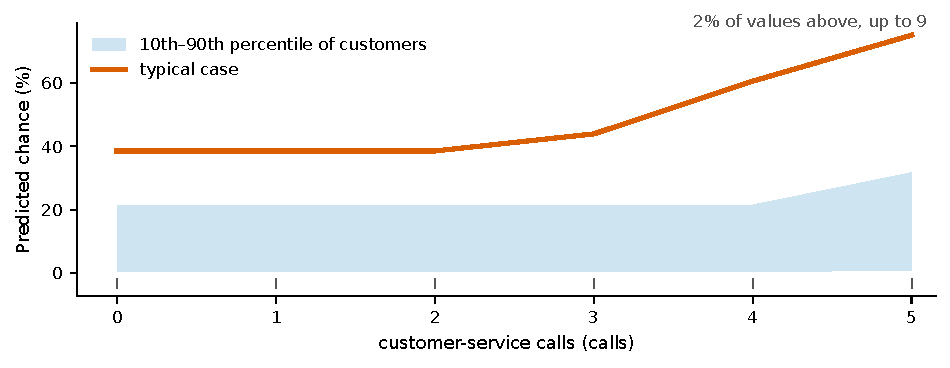
\includegraphics[width=\linewidth,height=0.88\textheight,keepaspectratio]{figures/churn100-s4-c3/ann_83-response.pdf}
\caption{Late rise in calls: Response curves through this part: the typical case (bold), the 10th to 90th percentile of individual customers (band), the fold or step point (dashed) with its spread across them (grey), and the observed values (ticks).}
\label{fig:churn100s4c3:plot-ann83-0}
\end{figure}
\begin{figure}[H]\centering
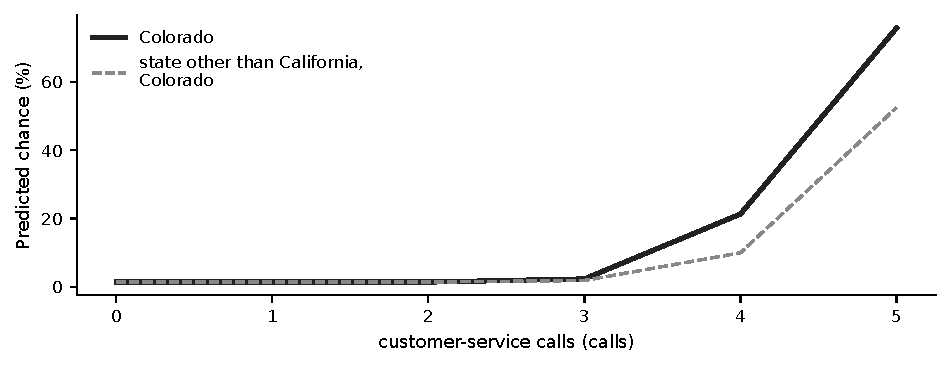
\includegraphics[width=\linewidth,height=0.88\textheight,keepaspectratio]{figures/churn100-s4-c3/ann_83-interaction.pdf}
\caption{Late rise in calls: How the effect differs between groups: one curve per group, for the typical case of each group.}
\label{fig:churn100s4c3:plot-ann83-1}
\end{figure}
\begin{figure}[H]\centering
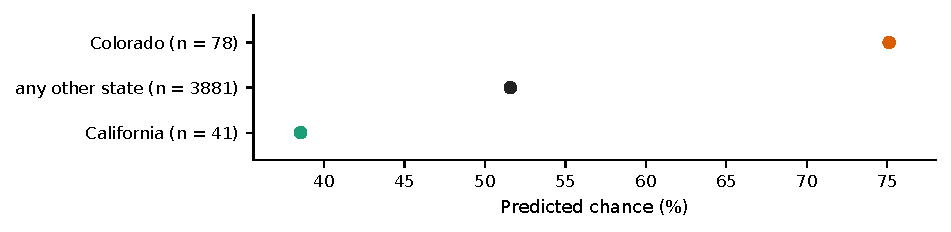
\includegraphics[width=\linewidth,height=0.88\textheight,keepaspectratio]{figures/churn100-s4-c3/ann_83-categories-small.pdf}
\caption{Late rise in calls: The predicted value for the typical case at each level, through this part (n = training customers; grey: fewer than 20).}
\label{fig:churn100s4c3:plot-ann83-2}
\end{figure}
\begin{figure}[H]\centering
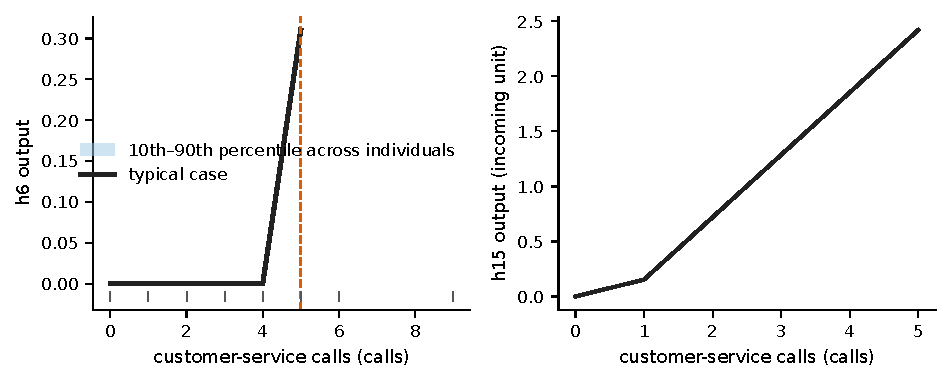
\includegraphics[width=\linewidth,height=0.88\textheight,keepaspectratio]{figures/churn100-s4-c3/ann_83-partial-5268.pdf}
\caption{Late rise in calls: This part's own output, unit h6 (combines 2 non-linear units), on its own scale (its activation), with every other input at the typical case; it is active for 134 of 4000. Bold: the typical case; band: 10th to 90th percentile across individuals; dashed: where it switches on; ticks: the data.}
\label{fig:churn100s4c3:plot-ann83-3}
\end{figure}
\begin{figure}[H]\centering
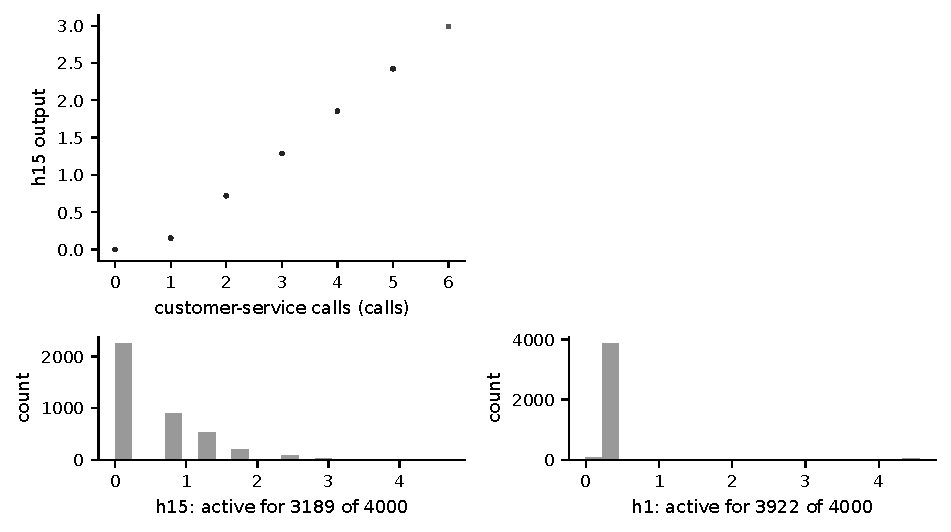
\includegraphics[width=\linewidth,height=0.88\textheight,keepaspectratio]{figures/churn100-s4-c3/ann_83-units.pdf}
\caption{Late rise in calls: This part's hidden units: each unit's output against its main numeric input (top) and how often it is active (bottom).}
\label{fig:churn100s4c3:plot-ann83-4}
\end{figure}
\par\smallskip\noindent{\small Technical detail: \ref{tech:ann83}.\par}
\subsubsection{Heavy daytime use}\label{rd:ann85}
\noindent{\footnotesize Part of: The whole model (\ref{rd:ann88}).\par}
\noindent{\small Figure~\ref{fig:churn100s4c3:parts-ann85} shows what feeds this part; Figure~\ref{fig:churn100s4c3:units-ann85} its units and every connection into them (dashed boxes: connections from or to other parts, drawn in their own sections).\par}
\begin{figure}[H]\centering
\resizebox{!}{\ifdim\height>0.5\textheight 0.5\textheight\else\height\fi}{%
\resizebox{\ifdim\width>\linewidth\linewidth\else\width\fi}{!}{%
\begin{tikzpicture}[
  font=\sffamily\scriptsize, >={Stealth[length=1.6mm]},
  inp/.style={draw, rounded corners=1pt, fill=white, inner sep=1.5pt, minimum height=3.2mm, anchor=east},
  abox/.style={draw, thick, rounded corners=2pt, align=center, inner sep=3pt, minimum height=6mm, text width=42mm},
  outp/.style={draw, double, rounded corners=2pt, fill=white, align=center, inner sep=3pt, text width=24mm},
  agg/.style={draw=black!55},
]
\node[inp] (i0) at (0,0.75) {voice-mail plan};
\node[inp] (i1) at (0,-0.0) {total daytime minutes};
\node[inp] (i2) at (0,-0.75) {total daytime charge};
\node[outp] (out) at (9.36,0) {Heavy daytime use};
\begin{scope}[on background layer]
\draw[->, agg, thin, dashed] (i0.east) -- (out.west);
\draw[->, agg, thin, dashed] (i1.east) -- (out.west);
\draw[->, agg, thin, dashed] (i2.east) -- (out.west);
\end{scope}
\end{tikzpicture}}}%
\caption{Heavy daytime use: what feeds it, one level down.}
\label{fig:churn100s4c3:parts-ann85}
\end{figure}
\begin{figure}[H]\centering
\resizebox{\ifdim\width>\linewidth\linewidth\else\width\fi}{!}{%
\definecolor{netup}{HTML}{D95F02}\definecolor{netdown}{HTML}{1B9E77}\definecolor{netmixed}{HTML}{7F7F7F}%
\begin{tikzpicture}[
  font=\sffamily\scriptsize, >={Stealth[length=1.4mm]},
  inp/.style={draw, circle, fill=white, minimum size=3.2mm, inner sep=0pt},
  hid/.style={draw, circle, fill=white, minimum size=5.2mm, inner sep=0.5pt, font=\sffamily\tiny},
  exitbox/.style={draw, thick, rectangle, fill=white, align=center, text width=17mm, minimum height=5mm, inner sep=1.5pt, font=\sffamily\tiny},
  sumbox/.style={draw, thick, dashed, rectangle, fill=white, align=center, text width=17mm, minimum height=5mm, inner sep=1.5pt, font=\sffamily\tiny},
  outp/.style={draw, thick, regular polygon, regular polygon sides=6, fill=white, minimum size=10mm, inner sep=0pt, font=\sffamily\tiny, align=center},
  stub/.style={draw, dashed, rounded corners=2pt, fill=white, align=center, inner sep=2pt, font=\sffamily\tiny, text width=15mm},
  inlab/.style={font=\sffamily\tiny, align=center, text width=15mm, inner sep=1pt, fill=white, fill opacity=0.8, text opacity=1},
  wpos/.style={draw=NavyBlue}, wneg/.style={draw=BrickRed}, wagg/.style={draw=black!45, line width=1.2pt},
  wmix/.style={draw=Plum},
]
\node[hid] (n3118) at (2.7,1.9) {h4};
\node[hid] (n10131) at (1.2,1.9) {h13};
\node[hid] (n4000) at (4.2,1.9) {h5};
\node[inp, draw=netup, very thick] (ninxxtotalxdayxminutes) at (4.5,0.0) {};
\path (ninxxtotalxdayxminutes.south) node[inlab, anchor=north] (labninxxtotalxdayxminutes) {total daytime minutes $\uparrow$};
\node[inp] (ninxxtotalxdayxcharge) at (2.7,0.0) {};
\path (ninxxtotalxdayxcharge.south) node[inlab, anchor=north] (labninxxtotalxdayxcharge) {total daytime charge};
\node[inp, draw=netdown, very thick] (ninxxvoicexmailxplan) at (0.9,0.0) {};
\path (ninxxvoicexmailxplan.south) node[inlab, anchor=north] (labninxxvoicexmailxplan) {a voice-mail plan $\downarrow$};
\node[stub] (ntoxxthexmodelxoutput) at (2.7,3.45) {to the model output};
\begin{scope}[on background layer]
\node[fit=(n3118) (n10131) (n4000) , inner sep=8pt, rounded corners=5pt, fill=Orchid!10, draw=Orchid!45] (clu0) {};
\draw[->, wpos, line width=0.50pt] (ninxxtotalxdayxminutes) -- (n4000);
\draw[->, wpos, line width=0.38pt] (ninxxtotalxdayxcharge) -- (n3118);
\draw[->, wpos, line width=0.53pt] (ninxxtotalxdayxminutes) -- (n10131);
\draw[->, wneg, line width=0.37pt] (ninxxvoicexmailxplan) -- (n10131);
\draw[->, wpos, line width=0.77pt] (n3118) -- (ntoxxthexmodelxoutput);
\draw[->, wpos, line width=0.77pt] (n4000) -- (ntoxxthexmodelxoutput);
\draw[->, wpos, line width=0.91pt] (n10131) -- (ntoxxthexmodelxoutput);
\end{scope}
\node[font=\sffamily\scriptsize\bfseries, text=Orchid!55!black, anchor=south west, inner sep=1pt, fill=white, fill opacity=0.85, text opacity=1] at (clu0.north west) {Heavy daytime use};
\end{tikzpicture}}%
\caption{Heavy daytime use: its units and every connection into them. Blue: positive weight (raises the score); red: negative weight (lowers it); thicker: larger weight. Orange outline and up arrow: raises the final prediction; teal and down arrow: lowers it; grey and double arrow: depends.}
\label{fig:churn100s4c3:units-ann85}
\end{figure}
\paragraph{Hypothesis.} This part raises the chance of leaving for heavy daytime users: daytime minutes add to it only above about 209 minutes, in an uneven way, and much less with a voice-mail plan.\,{\scriptsize\textcolor{NavyBlue}{[C100, C099]}}
\paragraph{Evidence.} This part acts on 1074 of 4000 training customers, 290 of whom left; for the typical customer it acts on, the chance is about 1\% without it and about 4\% with it.\,{\scriptsize\textcolor{NavyBlue}{[C102]}} Daytime minutes add to the chance only once they rise above about 209 minutes, in an uneven way: for a typical such customer, from about 1\% at 0 minutes to about 16\% at 271 minutes, flattening out near the bottom because the predicted chance cannot go much lower.\,{\scriptsize\textcolor{NavyBlue}{[C100]}} The rise is much larger without a voice-mail plan: from 112 to 249 daytime minutes the chance goes from about 1\% to about 6\% without one, but stays below 1\% with one, in an uneven way, flattening out near the bottom because the predicted chance cannot go much lower.\,{\scriptsize\textcolor{NavyBlue}{[C099]}} A voice-mail plan lowers it: for the typical customer it acts on, from about 4\% to about 2\%.\,{\scriptsize\textcolor{NavyBlue}{[C098]}} Its formula reproduces the part exactly on all 4000 training customers.\,{\scriptsize\textcolor{NavyBlue}{[C103]}}
\par\noindent{\small Evidence plots: Figure~\ref{fig:churn100s4c3:plot-ann85-0}, Figure~\ref{fig:churn100s4c3:plot-ann85-1}, Figure~\ref{fig:churn100s4c3:plot-ann85-2}, Figure~\ref{fig:churn100s4c3:plot-ann85-3}, Figure~\ref{fig:churn100s4c3:plot-ann85-4}, Figure~\ref{fig:churn100s4c3:plot-ann85-5}.\par}
\par\noindent{\small Figure~\ref{fig:churn100s4c3:plot-ann85-3} shows this part's own output, unit h13: it switches on at about 209 minutes of total daytime minutes, and is zero below.\par}
\par\noindent{\small Figure~\ref{fig:churn100s4c3:plot-ann85-4} shows this part's own output, unit h5: it switches on at about 223.9 minutes of total daytime minutes, and is zero below.\par}
\begin{figure}[H]\centering
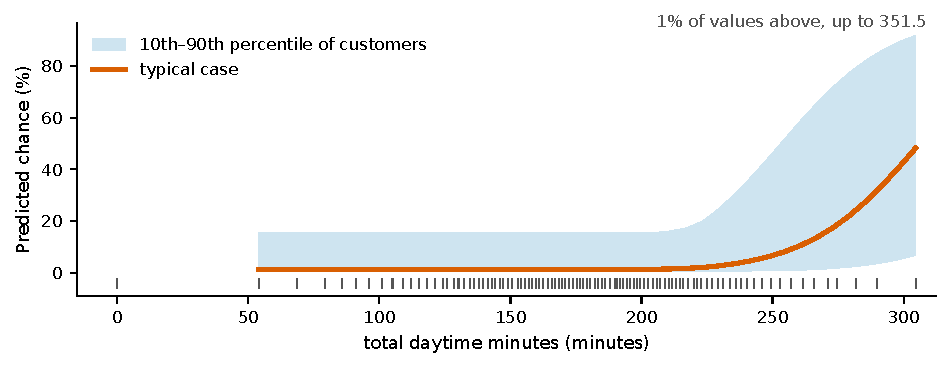
\includegraphics[width=\linewidth,height=0.88\textheight,keepaspectratio]{figures/churn100-s4-c3/ann_85-response.pdf}
\caption{Heavy daytime use: Response curves through this part: the typical case (bold), the 10th to 90th percentile of individual customers (band), the fold or step point (dashed) with its spread across them (grey), and the observed values (ticks).}
\label{fig:churn100s4c3:plot-ann85-0}
\end{figure}
\begin{figure}[H]\centering
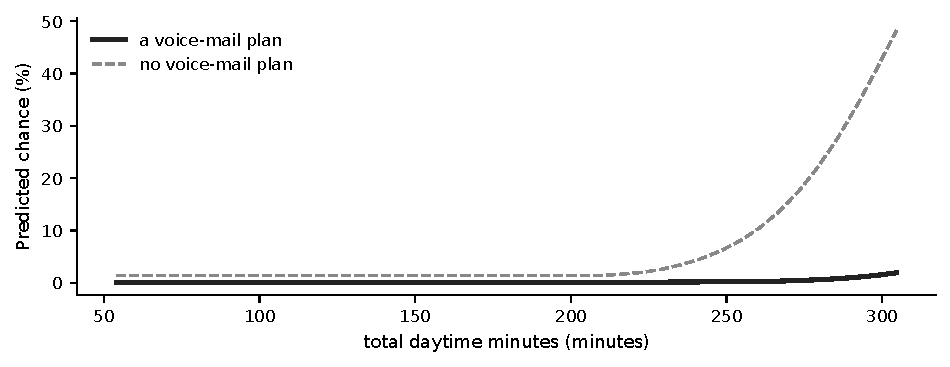
\includegraphics[width=\linewidth,height=0.88\textheight,keepaspectratio]{figures/churn100-s4-c3/ann_85-interaction.pdf}
\caption{Heavy daytime use: How the effect differs between groups: one curve per group, for the typical case of each group.}
\label{fig:churn100s4c3:plot-ann85-1}
\end{figure}
\begin{figure}[H]\centering
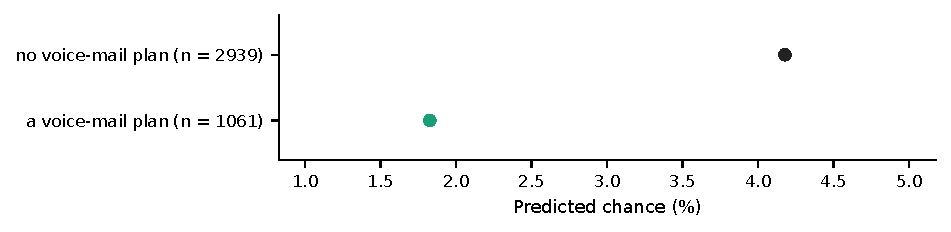
\includegraphics[width=\linewidth,height=0.88\textheight,keepaspectratio]{figures/churn100-s4-c3/ann_85-categories-small.pdf}
\caption{Heavy daytime use: The predicted value for the typical case at each level, through this part (n = training customers; grey: fewer than 20).}
\label{fig:churn100s4c3:plot-ann85-2}
\end{figure}
\begin{figure}[H]\centering
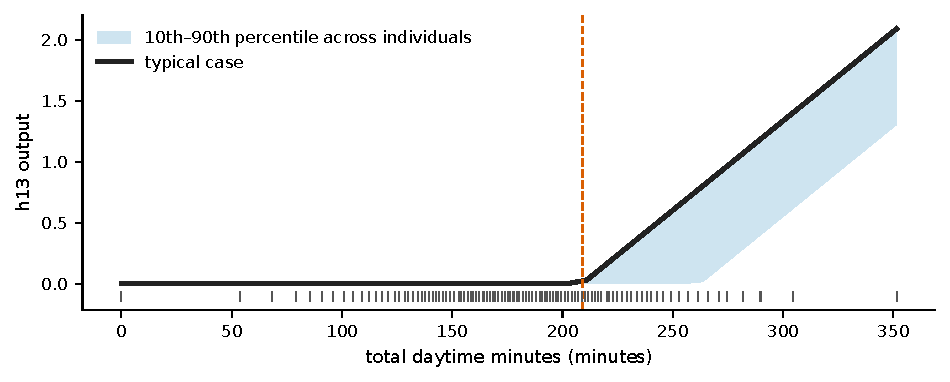
\includegraphics[width=\linewidth,height=0.88\textheight,keepaspectratio]{figures/churn100-s4-c3/ann_85-partial-10131.pdf}
\caption{Heavy daytime use: This part's own output, unit h13 (the output of 'Heavy daytime use'), on its own scale (its activation), with every other input at the typical case; it is active for 929 of 4000. Bold: the typical case; band: 10th to 90th percentile across individuals; dashed: where it switches on; ticks: the data.}
\label{fig:churn100s4c3:plot-ann85-3}
\end{figure}
\begin{figure}[H]\centering
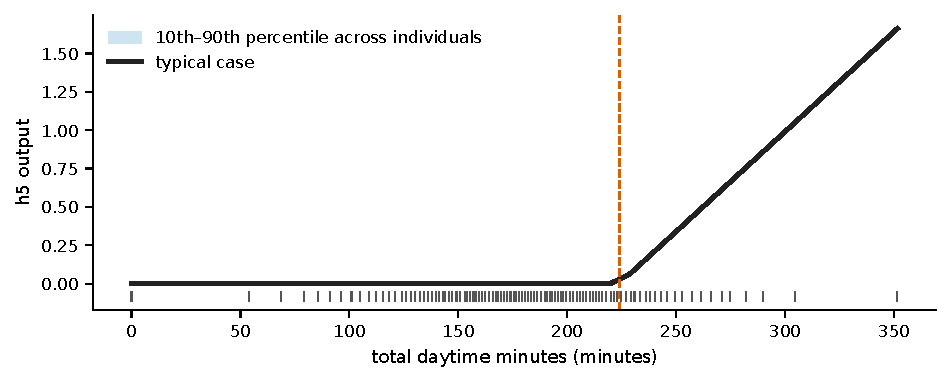
\includegraphics[width=\linewidth,height=0.88\textheight,keepaspectratio]{figures/churn100-s4-c3/ann_85-partial-4000.pdf}
\caption{Heavy daytime use: This part's own output, unit h5 (the output of 'Heavy daytime use'), on its own scale (its activation), with every other input at the typical case; it is active for 818 of 4000. Bold: the typical case; band: 10th to 90th percentile across individuals; dashed: where it switches on; ticks: the data.}
\label{fig:churn100s4c3:plot-ann85-4}
\end{figure}
\begin{figure}[H]\centering
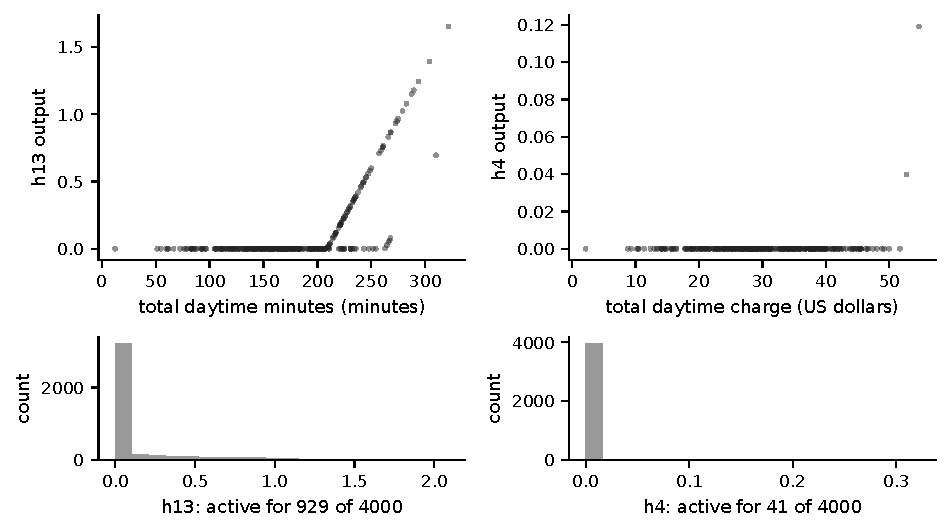
\includegraphics[width=\linewidth,height=0.88\textheight,keepaspectratio]{figures/churn100-s4-c3/ann_85-units.pdf}
\caption{Heavy daytime use: This part's hidden units: each unit's output against its main numeric input (top) and how often it is active (bottom).}
\label{fig:churn100s4c3:plot-ann85-5}
\end{figure}
\par\smallskip\noindent{\small Technical detail: \ref{tech:ann85}.\par}
\subsubsection{State units}\label{rd:ann86}
\noindent{\footnotesize Part of: The whole model (\ref{rd:ann88}).\par}
\noindent{\small Figure~\ref{fig:churn100s4c3:parts-ann86} shows what feeds this part; Figure~\ref{fig:churn100s4c3:units-ann86} its units and every connection into them (dashed boxes: connections from or to other parts, drawn in their own sections).\par}
\begin{figure}[H]\centering
\resizebox{!}{\ifdim\height>0.5\textheight 0.5\textheight\else\height\fi}{%
\resizebox{\ifdim\width>\linewidth\linewidth\else\width\fi}{!}{%
\begin{tikzpicture}[
  font=\sffamily\scriptsize, >={Stealth[length=1.6mm]},
  inp/.style={draw, rounded corners=1pt, fill=white, inner sep=1.5pt, minimum height=3.2mm, anchor=east},
  abox/.style={draw, thick, rounded corners=2pt, align=center, inner sep=3pt, minimum height=6mm, text width=42mm},
  outp/.style={draw, double, rounded corners=2pt, fill=white, align=center, inner sep=3pt, text width=24mm},
  agg/.style={draw=black!55},
]
\node[inp] (i0) at (0,0.375) {state};
\node[inp] (i1) at (0,-0.375) {total daytime calls};
\node[outp] (out) at (9.36,0) {State units};
\begin{scope}[on background layer]
\draw[->, agg, thin, dashed] (i0.east) -- (out.west);
\draw[->, agg, thin, dashed] (i1.east) -- (out.west);
\end{scope}
\end{tikzpicture}}}%
\caption{State units: what feeds it, one level down.}
\label{fig:churn100s4c3:parts-ann86}
\end{figure}
\begin{figure}[H]\centering
\resizebox{\ifdim\width>\linewidth\linewidth\else\width\fi}{!}{%
\definecolor{netup}{HTML}{D95F02}\definecolor{netdown}{HTML}{1B9E77}\definecolor{netmixed}{HTML}{7F7F7F}%
\begin{tikzpicture}[
  font=\sffamily\scriptsize, >={Stealth[length=1.4mm]},
  inp/.style={draw, circle, fill=white, minimum size=3.2mm, inner sep=0pt},
  hid/.style={draw, circle, fill=white, minimum size=5.2mm, inner sep=0.5pt, font=\sffamily\tiny},
  exitbox/.style={draw, thick, rectangle, fill=white, align=center, text width=17mm, minimum height=5mm, inner sep=1.5pt, font=\sffamily\tiny},
  sumbox/.style={draw, thick, dashed, rectangle, fill=white, align=center, text width=17mm, minimum height=5mm, inner sep=1.5pt, font=\sffamily\tiny},
  outp/.style={draw, thick, regular polygon, regular polygon sides=6, fill=white, minimum size=10mm, inner sep=0pt, font=\sffamily\tiny, align=center},
  stub/.style={draw, dashed, rounded corners=2pt, fill=white, align=center, inner sep=2pt, font=\sffamily\tiny, text width=15mm},
  inlab/.style={font=\sffamily\tiny, align=center, text width=15mm, inner sep=1pt, fill=white, fill opacity=0.8, text opacity=1},
  wpos/.style={draw=NavyBlue}, wneg/.style={draw=BrickRed}, wagg/.style={draw=black!45, line width=1.2pt},
  wmix/.style={draw=Plum},
]
\node[hid] (n11361) at (0.35,1.9) {h14};
\node[hid] (n13068) at (4.85,1.9) {h17};
\node[hid] (n12690) at (1.85,1.9) {h16};
\node[hid] (n1390) at (6.35,1.9) {h3};
\node[hid] (n15904) at (5.6,3.25) {h20};
\node[hid] (n1295) at (3.35,1.9) {h2};
\node[hid] (n15490) at (9.35,1.9) {h19};
\node[hid] (n17102) at (10.85,1.9) {h21};
\node[hid] (n5533) at (7.1,3.25) {h7};
\node[hid] (n7872) at (8.6,3.25) {h10};
\node[hid] (n15362) at (7.85,1.9) {h18};
\node[hid] (n5786) at (12.35,1.9) {h8};
\node[hid] (n9954) at (13.85,1.9) {h12};
\node[inp, draw=netmixed, very thick] (ngrpxxstate) at (6.2,0.0) {};
\path (ngrpxxstate.south) node[inlab, anchor=north] (labngrpxxstate) {state (31 of 51 used) $\updownarrow$};
\node[inp, draw=netup, very thick] (ninxxtotalxdayxcalls) at (8.0,0.0) {};
\path (ninxxtotalxdayxcalls.south) node[inlab, anchor=north] (labninxxtotalxdayxcalls) {total daytime calls $\uparrow$};
\node[stub] (ntoxxthexmodelxoutput) at (7.1,4.8) {to the model output};
\begin{scope}[on background layer]
\node[fit=(n11361) (n13068) (n12690) (n1390) (n15904) (n1295) (n15490) (n17102) (n5533) (n7872) (n15362) (n5786) (n9954) , inner sep=8pt, rounded corners=5pt, fill=Goldenrod!10, draw=Goldenrod!45] (clu0) {};
\draw[->, wpos, line width=0.61pt] (n1295) -- (n7872);
\draw[->, wpos, line width=0.48pt] (n5786) -- (n5533);
\draw[->, wpos, line width=0.60pt] (n15490) -- (n15904);
\draw[->, wneg, line width=0.25pt] (ninxxtotalxdayxcalls) -- (n5533);
\draw[->, wneg, line width=0.64pt] (n1295) -- (ntoxxthexmodelxoutput);
\draw[->, wneg, line width=0.66pt] (n1390) -- (ntoxxthexmodelxoutput);
\draw[->, wpos, line width=0.94pt] (n5533) -- (ntoxxthexmodelxoutput);
\draw[->, wneg, line width=0.44pt] (n5786) -- (ntoxxthexmodelxoutput);
\draw[->, wneg, line width=0.69pt] (n7872) -- (ntoxxthexmodelxoutput);
\draw[->, wpos, line width=0.27pt] (n9954) -- (ntoxxthexmodelxoutput);
\draw[->, wpos, line width=0.27pt] (n11361) -- (ntoxxthexmodelxoutput);
\draw[->, wneg, line width=0.26pt] (n12690) -- (ntoxxthexmodelxoutput);
\draw[->, wneg, line width=0.26pt] (n13068) -- (ntoxxthexmodelxoutput);
\draw[->, wpos, line width=0.27pt] (n15362) -- (ntoxxthexmodelxoutput);
\draw[->, wpos, line width=0.26pt] (n15490) -- (ntoxxthexmodelxoutput);
\draw[->, wpos, line width=0.27pt] (n15904) -- (ntoxxthexmodelxoutput);
\draw[->, wneg, line width=0.30pt] (n17102) -- (ntoxxthexmodelxoutput);
\draw[->, wpos, line width=0.60pt] (ngrpxxstate) -- node[pos=0.8, sloped, above, font=\sffamily\tiny, inner sep=1pt, fill=white, fill opacity=0.8, text opacity=1] {+1.01} (n9954);
\draw[->, wneg, line width=0.45pt] (ngrpxxstate) -- node[pos=0.8, sloped, above, font=\sffamily\tiny, inner sep=1pt, fill=white, fill opacity=0.8, text opacity=1] {-0.57} (n1390);
\draw[->, wmix, line width=0.78pt] (ngrpxxstate) -- node[pos=0.8, sloped, above, font=\sffamily\tiny, inner sep=1pt, fill=white, fill opacity=0.8, text opacity=1] {3 edges, -1.50 to +0.16} (n5786);
\draw[->, wpos, line width=0.60pt] (ngrpxxstate) -- node[pos=0.8, sloped, above, font=\sffamily\tiny, inner sep=1pt, fill=white, fill opacity=0.8, text opacity=1] {+1.00} (n15362);
\draw[->, wpos, line width=0.59pt] (ngrpxxstate) -- node[pos=0.8, sloped, above, font=\sffamily\tiny, inner sep=1pt, fill=white, fill opacity=0.8, text opacity=1] {+0.98} (n15490);
\draw[->, wpos, line width=0.60pt] (ngrpxxstate) -- node[pos=0.8, sloped, above, font=\sffamily\tiny, inner sep=1pt, fill=white, fill opacity=0.8, text opacity=1] {+0.99} (n17102);
\draw[->, wpos, line width=0.60pt] (ngrpxxstate) -- node[pos=0.8, sloped, above, font=\sffamily\tiny, inner sep=1pt, fill=white, fill opacity=0.8, text opacity=1] {+1.00} (n12690);
\draw[->, wpos, line width=0.61pt] (ngrpxxstate) -- node[pos=0.8, sloped, above, font=\sffamily\tiny, inner sep=1pt, fill=white, fill opacity=0.8, text opacity=1] {+1.02} (n13068);
\draw[->, wpos, line width=0.83pt] (ngrpxxstate) -- node[pos=0.8, sloped, above, font=\sffamily\tiny, inner sep=1pt, fill=white, fill opacity=0.8, text opacity=1] {+1.65} (n11361);
\draw[->, wneg, line width=0.70pt] (ngrpxxstate) -- node[pos=0.8, sloped, above, font=\sffamily\tiny, inner sep=1pt, fill=white, fill opacity=0.8, text opacity=1] {-1.28} (n1295);
\end{scope}
\node[font=\sffamily\scriptsize\bfseries, text=Goldenrod!55!black, anchor=south west, inner sep=1pt, fill=white, fill opacity=0.85, text opacity=1] at (clu0.north west) {State units};
\end{tikzpicture}}%
\caption{State units: its units and every connection into them. Blue: positive weight (raises the score); red: negative weight (lowers it); thicker: larger weight. Orange outline and up arrow: raises the final prediction; teal and down arrow: lowers it; grey and double arrow: depends.}
\label{fig:churn100s4c3:units-ann86}
\end{figure}
\paragraph{Hypothesis.} This part reads only the state: it raises the chance of leaving in Rhode Island, Vermont and Tennessee, and lowers it in Virginia and Nevada.\,{\scriptsize\textcolor{NavyBlue}{[C104, C105, C106, C107, C108]}}
\paragraph{Evidence.} This part reads only the state: it raises a typical customer's chance from about 1\% to about 12\% in Rhode Island, to about 3\% in Vermont and to about 2\% in Tennessee.\,{\scriptsize\textcolor{NavyBlue}{[C104, C105, C106]}} It lowers the chance to below 1\% in Virginia and in Nevada.\,{\scriptsize\textcolor{NavyBlue}{[C107, C108]}} Its formula reproduces the part exactly on all 4000 training customers.\,{\scriptsize\textcolor{NavyBlue}{[C116]}}
\par\noindent{\small Evidence plots: Figure~\ref{fig:churn100s4c3:plot-ann86-0}, Figure~\ref{fig:churn100s4c3:plot-ann86-1}.\par}
\begin{figure}[H]\centering
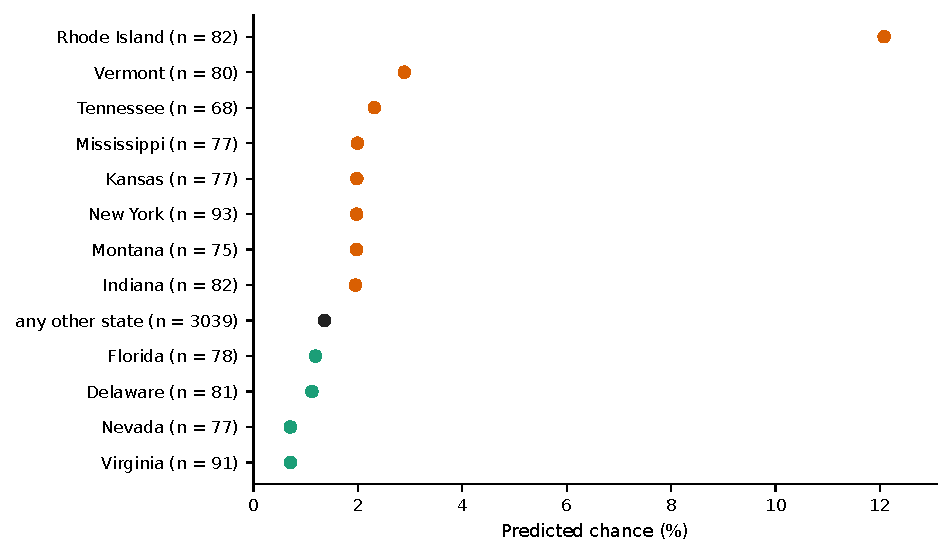
\includegraphics[width=\linewidth,height=0.88\textheight,keepaspectratio]{figures/churn100-s4-c3/ann_86-categories-C104.pdf}
\caption{State units: The predicted value for the typical case at each level, through this part (n = training customers; grey: fewer than 20).}
\label{fig:churn100s4c3:plot-ann86-0}
\end{figure}
\begin{figure}[H]\centering
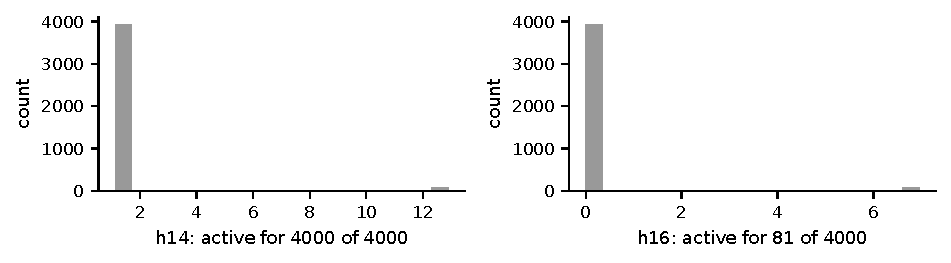
\includegraphics[width=\linewidth,height=0.88\textheight,keepaspectratio]{figures/churn100-s4-c3/ann_86-units.pdf}
\caption{State units: This part's hidden units: each unit's output against its main numeric input (top) and how often it is active (bottom).}
\label{fig:churn100s4c3:plot-ann86-1}
\end{figure}
\par\smallskip\noindent{\small Technical detail: \ref{tech:ann86}.\par}
\subsection{Not supported by the model}
\begin{itemize}\setlength\itemsep{0pt}\small
\item C101: threshold claim about total daytime charge in part ann\_\allowbreak{}85: not supported by the model (the effect past the fold is too small or not consistent across patients).
\item C121: threshold claim about number of calls to customer service in part ann\_\allowbreak{}83: not supported by the model (the effect past the fold is too small or not consistent across patients).
\end{itemize}
\clearpage\section*{Technical detail: churn100-s4-c3}
\addcontentsline{toc}{section}{Technical detail: churn100-s4-c3}
\noindent{\small The record behind each part: the original hypothesis, the closed form, and every claim with its estimate (log-odds and odds ratio), range across patients, n and test check.\par}
\renewcommand{\thesubsection}{T.\arabic{subsection}}\setcounter{subsection}{0}
\subsection{The whole model}\label{tech:ann88}
\noindent{\footnotesize Annotation ann\_\allowbreak{}88 (churn\_\allowbreak{}logit). Reads: state, account length, area code, international calling plan, voice-mail plan, number of voice-mail messages, total daytime minutes, total daytime calls, total daytime charge, total evening minutes, total evening calls, total evening charge, total night-time minutes, total night-time calls, total night-time charge, total international minutes, total international calls, total international charge, number of calls to customer service.\par}
\paragraph{Original hypothesis (unchanged).} Root: logit P(churn) = -1.35 + linear\_\allowbreak{}backbone (identity\_\allowbreak{}lin) + service\_\allowbreak{}calls (identity\_\allowbreak{}svc) + 1.48*3118 + 1.50*4000 + 1.89*10131 (day\_\allowbreak{}usage\_\allowbreak{}hinges) + the state\_\allowbreak{}offsets units (-1.11*1295 - 1.25*7872 - 1.17*1390 - 0.56*5786 + small terms; 5533 is never active), purely additive in the logit; the sigmoid is the only coupling. 30 inputs are unconnected (international minutes, calls and charge, night minutes/\allowbreak{}charge/\allowbreak{}calls,\allowbreak{} evening minutes and calls, area codes 408/510 and 20 state indicators) and have zero effect. Train AUC 0.8884, accuracy 0.8795; the mean predicted churn is 0.082 against a base rate of 0.1415 (the model ranks well but under-predicts). Performance sources (train): all children replaced by least-squares linear fits gives AUC 0.8352 (an L2 logistic regression refit on all 71 inputs gets 0.8433); restoring day\_\allowbreak{}usage\_\allowbreak{}hinges alone gives 0.8713, service\_\allowbreak{}calls alone 0.8657, both 0.8884; the state units restore nothing (exactly linear). So the gain over linear (+0.053) comes from the day-usage and service-call thresholds, which are complementary. Rare-category switches: state:11 -2.50 logit (73 rows, empirical -1.35); state:46 -1.46 net (80 rows, -0.91); state:47 +1.35 (72 rows, +0.92); state:0 -0.97 (56, -0.76); state:14 -0.94 (68, -0.53); state:29 -0.53 direct plus switching off the early service-call hinge (mean -0.78, down to -6.15 for many-call customers; 72 rows, -0.79); state:39 -0.55 net (82, -0.93: direct -2.85 mostly cancelled by the state units); state:33 +0.38 net (direct +1.05, unit -0.68); state:18 +0.36 (65 rows, empirical -0.48: opposite sign); state:4 switches off the late chain (41 rows, empirical +0.80).
\paragraph{Closed form.} Read through its parts (their formulas are in their own sections).
\paragraph{Split inputs.} To annotate the parts, the explanation split these inputs into copies (a refactoring step that does not change what the model computes); the diagrams draw each input once: customer-service calls (2 copies); total daytime calls (2 copies); a voice-mail plan (2 copies).
\paragraph{State: every level the model reads.} Whole-model change in the predicted chance for a typical customer when only the state changes from the reference; n = training customers in that level.\par\smallskip
{\scriptsize\rowcolors{2}{black!6}{white}
\begin{longtable}{@{}lllrlc@{}}
\toprule\rowcolor{white}
Claim & From & To & n & Chance & OK \\
\midrule\endhead
\bottomrule\endfoot
C004 & state other than Alaska, Georgia, Hawaii, Illinois, Indiana, Kansas, Louisiana, Massachusetts, Maine, Mississippi, Montana, North Carolina, North Dakota, Nebraska, Arizona, Nevada, New York, Oklahoma, Oregon, Pennsylvania, Rhode Island, California, South Carolina, Tennessee, Utah, Virginia, Vermont, Washington, Colorado, Delaware, Florida & Washington & 72 & 1\% to 5\% & \textcolor{OliveGreen}{yes} \\
C006 & state other than Alaska, Georgia, Hawaii, Illinois, Indiana, Kansas, Louisiana, Massachusetts, Maine, Mississippi, Montana, North Carolina, North Dakota, Nebraska, Arizona, Nevada, New York, Oklahoma, Oregon, Pennsylvania, Rhode Island, California, South Carolina, Tennessee, Utah, Virginia, Vermont, Washington, Colorado, Delaware, Florida & Maine & 86 & 1\% to 3\% & \textcolor{OliveGreen}{yes} \\
C010 & state other than Alaska, Georgia, Hawaii, Illinois, Indiana, Kansas, Louisiana, Massachusetts, Maine, Mississippi, Montana, North Carolina, North Dakota, Nebraska, Arizona, Nevada, New York, Oklahoma, Oregon, Pennsylvania, Rhode Island, California, South Carolina, Tennessee, Utah, Virginia, Vermont, Washington, Colorado, Delaware, Florida & Tennessee & 68 & 1\% to 2\% & \textcolor{OliveGreen}{yes} \\
C011 & state other than Alaska, Georgia, Hawaii, Illinois, Indiana, Kansas, Louisiana, Massachusetts, Maine, Mississippi, Montana, North Carolina, North Dakota, Nebraska, Arizona, Nevada, New York, Oklahoma, Oregon, Pennsylvania, Rhode Island, California, South Carolina, Tennessee, Utah, Virginia, Vermont, Washington, Colorado, Delaware, Florida & South Carolina & 66 & 1\% to 2\% & \textcolor{OliveGreen}{yes} \\
C017 & state other than Alaska, Georgia, Hawaii, Illinois, Indiana, Kansas, Louisiana, Massachusetts, Maine, Mississippi, Montana, North Carolina, North Dakota, Nebraska, Arizona, Nevada, New York, Oklahoma, Oregon, Pennsylvania, Rhode Island, California, South Carolina, Tennessee, Utah, Virginia, Vermont, Washington, Colorado, Delaware, Florida & Mississippi & 77 & 1\% to 2\% & \textcolor{OliveGreen}{yes} \\
C018 & state other than Alaska, Georgia, Hawaii, Illinois, Indiana, Kansas, Louisiana, Massachusetts, Maine, Mississippi, Montana, North Carolina, North Dakota, Nebraska, Arizona, Nevada, New York, Oklahoma, Oregon, Pennsylvania, Rhode Island, California, South Carolina, Tennessee, Utah, Virginia, Vermont, Washington, Colorado, Delaware, Florida & Nevada & 77 & 1\% to 2\% & \textcolor{OliveGreen}{yes} \\
C019 & state other than Alaska, Georgia, Hawaii, Illinois, Indiana, Kansas, Louisiana, Massachusetts, Maine, Mississippi, Montana, North Carolina, North Dakota, Nebraska, Arizona, Nevada, New York, Oklahoma, Oregon, Pennsylvania, Rhode Island, California, South Carolina, Tennessee, Utah, Virginia, Vermont, Washington, Colorado, Delaware, Florida & Kansas & 77 & 1\% to 2\% & \textcolor{OliveGreen}{yes} \\
C020 & state other than Alaska, Georgia, Hawaii, Illinois, Indiana, Kansas, Louisiana, Massachusetts, Maine, Mississippi, Montana, North Carolina, North Dakota, Nebraska, Arizona, Nevada, New York, Oklahoma, Oregon, Pennsylvania, Rhode Island, California, South Carolina, Tennessee, Utah, Virginia, Vermont, Washington, Colorado, Delaware, Florida & Montana & 75 & 1\% to 2\% & \textcolor{OliveGreen}{yes} \\
C021 & state other than Alaska, Georgia, Hawaii, Illinois, Indiana, Kansas, Louisiana, Massachusetts, Maine, Mississippi, Montana, North Carolina, North Dakota, Nebraska, Arizona, Nevada, New York, Oklahoma, Oregon, Pennsylvania, Rhode Island, California, South Carolina, Tennessee, Utah, Virginia, Vermont, Washington, Colorado, Delaware, Florida & New York & 93 & 1\% to 2\% & \textcolor{OliveGreen}{yes} \\
C022 & state other than Alaska, Georgia, Hawaii, Illinois, Indiana, Kansas, Louisiana, Massachusetts, Maine, Mississippi, Montana, North Carolina, North Dakota, Nebraska, Arizona, Nevada, New York, Oklahoma, Oregon, Pennsylvania, Rhode Island, California, South Carolina, Tennessee, Utah, Virginia, Vermont, Washington, Colorado, Delaware, Florida & Indiana & 82 & 1\% to 2\% & \textcolor{OliveGreen}{yes} \\
C023 & state other than Alaska, Georgia, Hawaii, Illinois, Indiana, Kansas, Louisiana, Massachusetts, Maine, Mississippi, Montana, North Carolina, North Dakota, Nebraska, Arizona, Nevada, New York, Oklahoma, Oregon, Pennsylvania, Rhode Island, California, South Carolina, Tennessee, Utah, Virginia, Vermont, Washington, Colorado, Delaware, Florida & Louisiana & 65 & 1\% to 2\% & \textcolor{OliveGreen}{yes} \\
C024 & state other than Alaska, Georgia, Hawaii, Illinois, Indiana, Kansas, Louisiana, Massachusetts, Maine, Mississippi, Montana, North Carolina, North Dakota, Nebraska, Arizona, Nevada, New York, Oklahoma, Oregon, Pennsylvania, Rhode Island, California, South Carolina, Tennessee, Utah, Virginia, Vermont, Washington, Colorado, Delaware, Florida & Utah & 89 & 1\% to 2\% & \textcolor{OliveGreen}{yes} \\
C026 & state other than Alaska, Georgia, Hawaii, Illinois, Indiana, Kansas, Louisiana, Massachusetts, Maine, Mississippi, Montana, North Carolina, North Dakota, Nebraska, Arizona, Nevada, New York, Oklahoma, Oregon, Pennsylvania, Rhode Island, California, South Carolina, Tennessee, Utah, Virginia, Vermont, Washington, Colorado, Delaware, Florida & Massachusetts & 86 & 1\% to 2\% & \textcolor{OliveGreen}{yes} \\
C032 & state other than Alaska, Georgia, Hawaii, Illinois, Indiana, Kansas, Louisiana, Massachusetts, Maine, Mississippi, Montana, North Carolina, North Dakota, Nebraska, Arizona, Nevada, New York, Oklahoma, Oregon, Pennsylvania, Rhode Island, California, South Carolina, Tennessee, Utah, Virginia, Vermont, Washington, Colorado, Delaware, Florida & Oregon & 84 & 1\% to 2\% & \textcolor{OliveGreen}{yes} \\
C035 & state other than Alaska, Georgia, Hawaii, Illinois, Indiana, Kansas, Louisiana, Massachusetts, Maine, Mississippi, Montana, North Carolina, North Dakota, Nebraska, Arizona, Nevada, New York, Oklahoma, Oregon, Pennsylvania, Rhode Island, California, South Carolina, Tennessee, Utah, Virginia, Vermont, Washington, Colorado, Delaware, Florida & North Dakota & 68 & 1\% to 1\% & \textcolor{OliveGreen}{yes} \\
C036 & state other than Alaska, Georgia, Hawaii, Illinois, Indiana, Kansas, Louisiana, Massachusetts, Maine, Mississippi, Montana, North Carolina, North Dakota, Nebraska, Arizona, Nevada, New York, Oklahoma, Oregon, Pennsylvania, Rhode Island, California, South Carolina, Tennessee, Utah, Virginia, Vermont, Washington, Colorado, Delaware, Florida & Oklahoma & 79 & 1\% to 1\% & \textcolor{OliveGreen}{yes} \\
C039 & state other than Alaska, Georgia, Hawaii, Illinois, Indiana, Kansas, Louisiana, Massachusetts, Maine, Mississippi, Montana, North Carolina, North Dakota, Nebraska, Arizona, Nevada, New York, Oklahoma, Oregon, Pennsylvania, Rhode Island, California, South Carolina, Tennessee, Utah, Virginia, Vermont, Washington, Colorado, Delaware, Florida & California & 41 & 1\% to 1\% & \textcolor{OliveGreen}{yes} \\
C040 & state other than Alaska, Georgia, Hawaii, Illinois, Indiana, Kansas, Louisiana, Massachusetts, Maine, Mississippi, Montana, North Carolina, North Dakota, Nebraska, Arizona, Nevada, New York, Oklahoma, Oregon, Pennsylvania, Rhode Island, California, South Carolina, Tennessee, Utah, Virginia, Vermont, Washington, Colorado, Delaware, Florida & Colorado & 78 & 1\% to 1\% & \textcolor{OliveGreen}{yes} \\
C037 & state other than Alaska, Georgia, Hawaii, Illinois, Indiana, Kansas, Louisiana, Massachusetts, Maine, Mississippi, Montana, North Carolina, North Dakota, Nebraska, Arizona, Nevada, New York, Oklahoma, Oregon, Pennsylvania, Rhode Island, California, South Carolina, Tennessee, Utah, Virginia, Vermont, Washington, Colorado, Delaware, Florida & Arizona & 73 & 1\% to 1\% & \textcolor{OliveGreen}{yes} \\
C034 & state other than Alaska, Georgia, Hawaii, Illinois, Indiana, Kansas, Louisiana, Massachusetts, Maine, Mississippi, Montana, North Carolina, North Dakota, Nebraska, Arizona, Nevada, New York, Oklahoma, Oregon, Pennsylvania, Rhode Island, California, South Carolina, Tennessee, Utah, Virginia, Vermont, Washington, Colorado, Delaware, Florida & North Carolina & 74 & 1\% to 1\% & \textcolor{OliveGreen}{yes} \\
C033 & state other than Alaska, Georgia, Hawaii, Illinois, Indiana, Kansas, Louisiana, Massachusetts, Maine, Mississippi, Montana, North Carolina, North Dakota, Nebraska, Arizona, Nevada, New York, Oklahoma, Oregon, Pennsylvania, Rhode Island, California, South Carolina, Tennessee, Utah, Virginia, Vermont, Washington, Colorado, Delaware, Florida & Delaware & 81 & 1\% to 1\% & \textcolor{OliveGreen}{yes} \\
C028 & state other than Alaska, Georgia, Hawaii, Illinois, Indiana, Kansas, Louisiana, Massachusetts, Maine, Mississippi, Montana, North Carolina, North Dakota, Nebraska, Arizona, Nevada, New York, Oklahoma, Oregon, Pennsylvania, Rhode Island, California, South Carolina, Tennessee, Utah, Virginia, Vermont, Washington, Colorado, Delaware, Florida & Florida & 78 & 1\% to 1\% & \textcolor{OliveGreen}{yes} \\
C027 & state other than Alaska, Georgia, Hawaii, Illinois, Indiana, Kansas, Louisiana, Massachusetts, Maine, Mississippi, Montana, North Carolina, North Dakota, Nebraska, Arizona, Nevada, New York, Oklahoma, Oregon, Pennsylvania, Rhode Island, California, South Carolina, Tennessee, Utah, Virginia, Vermont, Washington, Colorado, Delaware, Florida & Nebraska & 72 & 1\% to 1\% & \textcolor{OliveGreen}{yes} \\
C025 & state other than Alaska, Georgia, Hawaii, Illinois, Indiana, Kansas, Louisiana, Massachusetts, Maine, Mississippi, Montana, North Carolina, North Dakota, Nebraska, Arizona, Nevada, New York, Oklahoma, Oregon, Pennsylvania, Rhode Island, California, South Carolina, Tennessee, Utah, Virginia, Vermont, Washington, Colorado, Delaware, Florida & Rhode Island & 82 & 1\% to 1\% & \textcolor{OliveGreen}{yes} \\
C016 & state other than Alaska, Georgia, Hawaii, Illinois, Indiana, Kansas, Louisiana, Massachusetts, Maine, Mississippi, Montana, North Carolina, North Dakota, Nebraska, Arizona, Nevada, New York, Oklahoma, Oregon, Pennsylvania, Rhode Island, California, South Carolina, Tennessee, Utah, Virginia, Vermont, Washington, Colorado, Delaware, Florida & Georgia & 60 & 1\% to 1\% & \textcolor{OliveGreen}{yes} \\
C015 & state other than Alaska, Georgia, Hawaii, Illinois, Indiana, Kansas, Louisiana, Massachusetts, Maine, Mississippi, Montana, North Carolina, North Dakota, Nebraska, Arizona, Nevada, New York, Oklahoma, Oregon, Pennsylvania, Rhode Island, California, South Carolina, Tennessee, Utah, Virginia, Vermont, Washington, Colorado, Delaware, Florida & Virginia & 91 & 1\% to 1\% & \textcolor{OliveGreen}{yes} \\
C014 & state other than Alaska, Georgia, Hawaii, Illinois, Indiana, Kansas, Louisiana, Massachusetts, Maine, Mississippi, Montana, North Carolina, North Dakota, Nebraska, Arizona, Nevada, New York, Oklahoma, Oregon, Pennsylvania, Rhode Island, California, South Carolina, Tennessee, Utah, Virginia, Vermont, Washington, Colorado, Delaware, Florida & Pennsylvania & 56 & 1\% to 1\% & \textcolor{OliveGreen}{yes} \\
C013 & state other than Alaska, Georgia, Hawaii, Illinois, Indiana, Kansas, Louisiana, Massachusetts, Maine, Mississippi, Montana, North Carolina, North Dakota, Nebraska, Arizona, Nevada, New York, Oklahoma, Oregon, Pennsylvania, Rhode Island, California, South Carolina, Tennessee, Utah, Virginia, Vermont, Washington, Colorado, Delaware, Florida & Illinois & 68 & 1\% to 1\% & \textcolor{OliveGreen}{yes} \\
C012 & state other than Alaska, Georgia, Hawaii, Illinois, Indiana, Kansas, Louisiana, Massachusetts, Maine, Mississippi, Montana, North Carolina, North Dakota, Nebraska, Arizona, Nevada, New York, Oklahoma, Oregon, Pennsylvania, Rhode Island, California, South Carolina, Tennessee, Utah, Virginia, Vermont, Washington, Colorado, Delaware, Florida & Alaska & 56 & 1\% to 1\% & \textcolor{OliveGreen}{yes} \\
C009 & state other than Alaska, Georgia, Hawaii, Illinois, Indiana, Kansas, Louisiana, Massachusetts, Maine, Mississippi, Montana, North Carolina, North Dakota, Nebraska, Arizona, Nevada, New York, Oklahoma, Oregon, Pennsylvania, Rhode Island, California, South Carolina, Tennessee, Utah, Virginia, Vermont, Washington, Colorado, Delaware, Florida & Vermont & 80 & 1\% to $<$1\% & \textcolor{OliveGreen}{yes} \\
C007 & state other than Alaska, Georgia, Hawaii, Illinois, Indiana, Kansas, Louisiana, Massachusetts, Maine, Mississippi, Montana, North Carolina, North Dakota, Nebraska, Arizona, Nevada, New York, Oklahoma, Oregon, Pennsylvania, Rhode Island, California, South Carolina, Tennessee, Utah, Virginia, Vermont, Washington, Colorado, Delaware, Florida & Hawaii & 73 & 1\% to $<$1\% & \textcolor{OliveGreen}{yes} \\
\end{longtable}}
\paragraph{Evidence table} (next page, landscape).
\begin{landscape}
{\scriptsize\setlength{\tabcolsep}{3pt}\renewcommand{\arraystretch}{1.15}
\rowcolors{2}{black!6}{white}
\begin{longtable}{@{}l>{\raggedright\arraybackslash}p{0.36\linewidth}>{\raggedright\arraybackslash}p{0.14\linewidth}rrr>{\raggedright\arraybackslash}p{0.06\linewidth}>{\raggedright\arraybackslash}p{0.17\linewidth}c@{}}
\toprule\rowcolor{white}
ID & What is checked & Risk, typical patient & Log-odds & OR & Range (p10--p90) & n & Test check & OK \\
\midrule\endfirsthead
\toprule\rowcolor{white}
ID & What is checked & Risk, typical patient & Log-odds & OR & Range (p10--p90) & n & Test check & OK \\
\midrule\endhead
\bottomrule\endfoot
C001 & direction: international calling plan: no international plan to an international plan (whole model) \newline{\itshape shape: categorical; highest to lowest: an international plan, no international plan} & 1\% to 18\% & 2.74 & 15.6 & 2.74 to 2.74 & 3620, 380 & agrees; AUC gain 0.066 [0.035, 0.098] & \textcolor{OliveGreen}{yes} \\
C002 & direction: voice-mail messages: 0 messages to 32 messages (whole model) \newline{\itshape shape: steady; 100\% of patients same; verified; risk saturates near 0\%} & 1\% to 6\% & 1.61 & 5.00 & 1.61 to 1.61 & 4000 & agrees; AUC gain 0.014 [0.0002, 0.029] & \textcolor{OliveGreen}{yes} \\
C003 & direction: total daytime minutes: 112 minutes to 249 minutes (whole model) \newline{\itshape shape: accelerating; 100\% of patients same; fallback; risk saturates near 0\%} & 1\% to 6\% & 1.30 & 3.67 & 0.49 to 1.59 & 4000 & agrees; AUC gain 0.074 [0.044, 0.105] & \textcolor{OliveGreen}{yes} \\
C004 & direction: state: state other than Alaska, Georgia, Hawaii, Illinois, Indiana, Kansas, Louisiana, Massachusetts, Maine, Mississippi, Montana, North Carolina, North Dakota, Nebraska, Arizona, Nevada, New York, Oklahoma, Oregon, Pennsylvania, Rhode Island, California, South Carolina, Tennessee, Utah, Virginia, Vermont, Washington, Colorado, Delaware, Florida to Washington (whole model) \newline{\itshape shape: categorical; highest to lowest: Washington, Maine, Tennessee, South Carolina, Mississippi, Nevada ...} & 1\% to 5\% & 1.35 & 3.86 & 1.35 to 1.35 & 1693, 72 & disagrees; AUC gain -0.013 [-0.028, -0.0007] & \textcolor{OliveGreen}{yes} \\
C005 & direction: total evening charge: 11.76 US dollars to 22.57 US dollars (whole model) \newline{\itshape shape: steady; 100\% of patients same; verified; risk saturates near 0\%} & 1\% to 2\% & 1.01 & 2.73 & 1.01 to 1.01 & 4000 & agrees; AUC gain 0.014 [0.003, 0.026] & \textcolor{OliveGreen}{yes} \\
C006 & direction: state: state other than Alaska, Georgia, Hawaii, Illinois, Indiana, Kansas, Louisiana, Massachusetts, Maine, Mississippi, Montana, North Carolina, North Dakota, Nebraska, Arizona, Nevada, New York, Oklahoma, Oregon, Pennsylvania, Rhode Island, California, South Carolina, Tennessee, Utah, Virginia, Vermont, Washington, Colorado, Delaware, Florida to Maine (whole model) \newline{\itshape shape: categorical; highest to lowest: Washington, Maine, Tennessee, South Carolina, Mississippi, Nevada ...} & 1\% to 3\% & 0.71 & 2.04 & 0.71 to 0.71 & 1693, 86 & disagrees; AUC gain -0.013 [-0.028, -0.0007] & \textcolor{OliveGreen}{yes} \\
C007 & direction: state: state other than Alaska, Georgia, Hawaii, Illinois, Indiana, Kansas, Louisiana, Massachusetts, Maine, Mississippi, Montana, North Carolina, North Dakota, Nebraska, Arizona, Nevada, New York, Oklahoma, Oregon, Pennsylvania, Rhode Island, California, South Carolina, Tennessee, Utah, Virginia, Vermont, Washington, Colorado, Delaware, Florida to Hawaii (whole model) \newline{\itshape shape: categorical; highest to lowest: Washington, Maine, Tennessee, South Carolina, Mississippi, Nevada ...} & 1\% to $<$1\% & -2.50 & 0.08 & -2.50 to -2.50 & 1693, 73 & disagrees; AUC gain -0.013 [-0.028, -0.0007] & \textcolor{OliveGreen}{yes} \\
C008 & direction: voice-mail plan: no voice-mail plan to a voice-mail plan (whole model) \newline{\itshape shape: categorical; highest to lowest: no voice-mail plan, a voice-mail plan} & 1\% to $<$1\% & -2.62 & 0.07 & -3.50 to -2.38 & 2939, 1061 & agrees; AUC gain 0.049 [0.028, 0.072] & \textcolor{OliveGreen}{yes} \\
C009 & direction: state: state other than Alaska, Georgia, Hawaii, Illinois, Indiana, Kansas, Louisiana, Massachusetts, Maine, Mississippi, Montana, North Carolina, North Dakota, Nebraska, Arizona, Nevada, New York, Oklahoma, Oregon, Pennsylvania, Rhode Island, California, South Carolina, Tennessee, Utah, Virginia, Vermont, Washington, Colorado, Delaware, Florida to Vermont (whole model) \newline{\itshape shape: categorical; highest to lowest: Washington, Maine, Tennessee, South Carolina, Mississippi, Nevada ...} & 1\% to $<$1\% & -1.46 & 0.23 & -1.46 to -1.46 & 1693, 80 & disagrees; AUC gain -0.013 [-0.028, -0.0007] & \textcolor{OliveGreen}{yes} \\
C010 & direction: state: state other than Alaska, Georgia, Hawaii, Illinois, Indiana, Kansas, Louisiana, Massachusetts, Maine, Mississippi, Montana, North Carolina, North Dakota, Nebraska, Arizona, Nevada, New York, Oklahoma, Oregon, Pennsylvania, Rhode Island, California, South Carolina, Tennessee, Utah, Virginia, Vermont, Washington, Colorado, Delaware, Florida to Tennessee (whole model) \newline{\itshape shape: categorical; highest to lowest: Washington, Maine, Tennessee, South Carolina, Mississippi, Nevada ...} & 1\% to 2\% & 0.54 & 1.72 & 0.54 to 0.54 & 1693, 68 & disagrees; AUC gain -0.013 [-0.028, -0.0007] & \textcolor{OliveGreen}{yes} \\
C011 & direction: state: state other than Alaska, Georgia, Hawaii, Illinois, Indiana, Kansas, Louisiana, Massachusetts, Maine, Mississippi, Montana, North Carolina, North Dakota, Nebraska, Arizona, Nevada, New York, Oklahoma, Oregon, Pennsylvania, Rhode Island, California, South Carolina, Tennessee, Utah, Virginia, Vermont, Washington, Colorado, Delaware, Florida to South Carolina (whole model) \newline{\itshape shape: categorical; highest to lowest: Washington, Maine, Tennessee, South Carolina, Mississippi, Nevada ...} & 1\% to 2\% & 0.54 & 1.71 & 0.54 to 0.54 & 1693, 66 & disagrees; AUC gain -0.013 [-0.028, -0.0007] & \textcolor{OliveGreen}{yes} \\
C012 & direction: state: state other than Alaska, Georgia, Hawaii, Illinois, Indiana, Kansas, Louisiana, Massachusetts, Maine, Mississippi, Montana, North Carolina, North Dakota, Nebraska, Arizona, Nevada, New York, Oklahoma, Oregon, Pennsylvania, Rhode Island, California, South Carolina, Tennessee, Utah, Virginia, Vermont, Washington, Colorado, Delaware, Florida to Alaska (whole model) \newline{\itshape shape: categorical; highest to lowest: Washington, Maine, Tennessee, South Carolina, Mississippi, Nevada ...} & 1\% to 1\% & -0.97 & 0.38 & -0.97 to -0.97 & 1693, 56 & disagrees; AUC gain -0.013 [-0.028, -0.0007] & \textcolor{OliveGreen}{yes} \\
C013 & direction: state: state other than Alaska, Georgia, Hawaii, Illinois, Indiana, Kansas, Louisiana, Massachusetts, Maine, Mississippi, Montana, North Carolina, North Dakota, Nebraska, Arizona, Nevada, New York, Oklahoma, Oregon, Pennsylvania, Rhode Island, California, South Carolina, Tennessee, Utah, Virginia, Vermont, Washington, Colorado, Delaware, Florida to Illinois (whole model) \newline{\itshape shape: categorical; highest to lowest: Washington, Maine, Tennessee, South Carolina, Mississippi, Nevada ...} & 1\% to 1\% & -0.94 & 0.39 & -0.94 to -0.94 & 1693, 68 & disagrees; AUC gain -0.013 [-0.028, -0.0007] & \textcolor{OliveGreen}{yes} \\
C014 & direction: state: state other than Alaska, Georgia, Hawaii, Illinois, Indiana, Kansas, Louisiana, Massachusetts, Maine, Mississippi, Montana, North Carolina, North Dakota, Nebraska, Arizona, Nevada, New York, Oklahoma, Oregon, Pennsylvania, Rhode Island, California, South Carolina, Tennessee, Utah, Virginia, Vermont, Washington, Colorado, Delaware, Florida to Pennsylvania (whole model) \newline{\itshape shape: categorical; highest to lowest: Washington, Maine, Tennessee, South Carolina, Mississippi, Nevada ...} & 1\% to 1\% & -0.77 & 0.46 & -0.77 to -0.77 & 1693, 56 & disagrees; AUC gain -0.013 [-0.028, -0.0007] & \textcolor{OliveGreen}{yes} \\
C015 & direction: state: state other than Alaska, Georgia, Hawaii, Illinois, Indiana, Kansas, Louisiana, Massachusetts, Maine, Mississippi, Montana, North Carolina, North Dakota, Nebraska, Arizona, Nevada, New York, Oklahoma, Oregon, Pennsylvania, Rhode Island, California, South Carolina, Tennessee, Utah, Virginia, Vermont, Washington, Colorado, Delaware, Florida to Virginia (whole model) \newline{\itshape shape: categorical; highest to lowest: Washington, Maine, Tennessee, South Carolina, Mississippi, Nevada ...} & 1\% to 1\% & -0.66 & 0.52 & -0.66 to -0.66 & 1693, 91 & disagrees; AUC gain -0.013 [-0.028, -0.0007] & \textcolor{OliveGreen}{yes} \\
C016 & direction: state: state other than Alaska, Georgia, Hawaii, Illinois, Indiana, Kansas, Louisiana, Massachusetts, Maine, Mississippi, Montana, North Carolina, North Dakota, Nebraska, Arizona, Nevada, New York, Oklahoma, Oregon, Pennsylvania, Rhode Island, California, South Carolina, Tennessee, Utah, Virginia, Vermont, Washington, Colorado, Delaware, Florida to Georgia (whole model) \newline{\itshape shape: categorical; highest to lowest: Washington, Maine, Tennessee, South Carolina, Mississippi, Nevada ...} & 1\% to 1\% & -0.64 & 0.53 & -0.64 to -0.64 & 1693, 60 & disagrees; AUC gain -0.013 [-0.028, -0.0007] & \textcolor{OliveGreen}{yes} \\
C017 & direction: state: state other than Alaska, Georgia, Hawaii, Illinois, Indiana, Kansas, Louisiana, Massachusetts, Maine, Mississippi, Montana, North Carolina, North Dakota, Nebraska, Arizona, Nevada, New York, Oklahoma, Oregon, Pennsylvania, Rhode Island, California, South Carolina, Tennessee, Utah, Virginia, Vermont, Washington, Colorado, Delaware, Florida to Mississippi (whole model) \newline{\itshape shape: categorical; highest to lowest: Washington, Maine, Tennessee, South Carolina, Mississippi, Nevada ...} & 1\% to 2\% & 0.39 & 1.47 & 0.39 to 0.39 & 1693, 77 & disagrees; AUC gain -0.013 [-0.028, -0.0007] & \textcolor{OliveGreen}{yes} \\
C018 & direction: state: state other than Alaska, Georgia, Hawaii, Illinois, Indiana, Kansas, Louisiana, Massachusetts, Maine, Mississippi, Montana, North Carolina, North Dakota, Nebraska, Arizona, Nevada, New York, Oklahoma, Oregon, Pennsylvania, Rhode Island, California, South Carolina, Tennessee, Utah, Virginia, Vermont, Washington, Colorado, Delaware, Florida to Nevada (whole model) \newline{\itshape shape: categorical; highest to lowest: Washington, Maine, Tennessee, South Carolina, Mississippi, Nevada ...} & 1\% to 2\% & 0.38 & 1.47 & 0.38 to 0.38 & 1693, 77 & disagrees; AUC gain -0.013 [-0.028, -0.0007] & \textcolor{OliveGreen}{yes} \\
C019 & direction: state: state other than Alaska, Georgia, Hawaii, Illinois, Indiana, Kansas, Louisiana, Massachusetts, Maine, Mississippi, Montana, North Carolina, North Dakota, Nebraska, Arizona, Nevada, New York, Oklahoma, Oregon, Pennsylvania, Rhode Island, California, South Carolina, Tennessee, Utah, Virginia, Vermont, Washington, Colorado, Delaware, Florida to Kansas (whole model) \newline{\itshape shape: categorical; highest to lowest: Washington, Maine, Tennessee, South Carolina, Mississippi, Nevada ...} & 1\% to 2\% & 0.38 & 1.46 & 0.38 to 0.38 & 1693, 77 & disagrees; AUC gain -0.013 [-0.028, -0.0007] & \textcolor{OliveGreen}{yes} \\
C020 & direction: state: state other than Alaska, Georgia, Hawaii, Illinois, Indiana, Kansas, Louisiana, Massachusetts, Maine, Mississippi, Montana, North Carolina, North Dakota, Nebraska, Arizona, Nevada, New York, Oklahoma, Oregon, Pennsylvania, Rhode Island, California, South Carolina, Tennessee, Utah, Virginia, Vermont, Washington, Colorado, Delaware, Florida to Montana (whole model) \newline{\itshape shape: categorical; highest to lowest: Washington, Maine, Tennessee, South Carolina, Mississippi, Nevada ...} & 1\% to 2\% & 0.38 & 1.46 & 0.38 to 0.38 & 1693, 75 & disagrees; AUC gain -0.013 [-0.028, -0.0007] & \textcolor{OliveGreen}{yes} \\
C021 & direction: state: state other than Alaska, Georgia, Hawaii, Illinois, Indiana, Kansas, Louisiana, Massachusetts, Maine, Mississippi, Montana, North Carolina, North Dakota, Nebraska, Arizona, Nevada, New York, Oklahoma, Oregon, Pennsylvania, Rhode Island, California, South Carolina, Tennessee, Utah, Virginia, Vermont, Washington, Colorado, Delaware, Florida to New York (whole model) \newline{\itshape shape: categorical; highest to lowest: Washington, Maine, Tennessee, South Carolina, Mississippi, Nevada ...} & 1\% to 2\% & 0.38 & 1.46 & 0.38 to 0.38 & 1693, 93 & disagrees; AUC gain -0.013 [-0.028, -0.0007] & \textcolor{OliveGreen}{yes} \\
C022 & direction: state: state other than Alaska, Georgia, Hawaii, Illinois, Indiana, Kansas, Louisiana, Massachusetts, Maine, Mississippi, Montana, North Carolina, North Dakota, Nebraska, Arizona, Nevada, New York, Oklahoma, Oregon, Pennsylvania, Rhode Island, California, South Carolina, Tennessee, Utah, Virginia, Vermont, Washington, Colorado, Delaware, Florida to Indiana (whole model) \newline{\itshape shape: categorical; highest to lowest: Washington, Maine, Tennessee, South Carolina, Mississippi, Nevada ...} & 1\% to 2\% & 0.37 & 1.45 & 0.37 to 0.37 & 1693, 82 & disagrees; AUC gain -0.013 [-0.028, -0.0007] & \textcolor{OliveGreen}{yes} \\
C023 & direction: state: state other than Alaska, Georgia, Hawaii, Illinois, Indiana, Kansas, Louisiana, Massachusetts, Maine, Mississippi, Montana, North Carolina, North Dakota, Nebraska, Arizona, Nevada, New York, Oklahoma, Oregon, Pennsylvania, Rhode Island, California, South Carolina, Tennessee, Utah, Virginia, Vermont, Washington, Colorado, Delaware, Florida to Louisiana (whole model) \newline{\itshape shape: categorical; highest to lowest: Washington, Maine, Tennessee, South Carolina, Mississippi, Nevada ...} & 1\% to 2\% & 0.36 & 1.44 & 0.36 to 0.36 & 1693, 65 & disagrees; AUC gain -0.013 [-0.028, -0.0007] & \textcolor{OliveGreen}{yes} \\
C024 & direction: state: state other than Alaska, Georgia, Hawaii, Illinois, Indiana, Kansas, Louisiana, Massachusetts, Maine, Mississippi, Montana, North Carolina, North Dakota, Nebraska, Arizona, Nevada, New York, Oklahoma, Oregon, Pennsylvania, Rhode Island, California, South Carolina, Tennessee, Utah, Virginia, Vermont, Washington, Colorado, Delaware, Florida to Utah (whole model) \newline{\itshape shape: categorical; highest to lowest: Washington, Maine, Tennessee, South Carolina, Mississippi, Nevada ...} & 1\% to 2\% & 0.36 & 1.44 & 0.36 to 0.36 & 1693, 89 & disagrees; AUC gain -0.013 [-0.028, -0.0007] & \textcolor{OliveGreen}{yes} \\
C025 & direction: state: state other than Alaska, Georgia, Hawaii, Illinois, Indiana, Kansas, Louisiana, Massachusetts, Maine, Mississippi, Montana, North Carolina, North Dakota, Nebraska, Arizona, Nevada, New York, Oklahoma, Oregon, Pennsylvania, Rhode Island, California, South Carolina, Tennessee, Utah, Virginia, Vermont, Washington, Colorado, Delaware, Florida to Rhode Island (whole model) \newline{\itshape shape: categorical; highest to lowest: Washington, Maine, Tennessee, South Carolina, Mississippi, Nevada ...} & 1\% to 1\% & -0.55 & 0.58 & -0.55 to -0.55 & 1693, 82 & disagrees; AUC gain -0.013 [-0.028, -0.0007] & \textcolor{OliveGreen}{yes} \\
C026 & direction: state: state other than Alaska, Georgia, Hawaii, Illinois, Indiana, Kansas, Louisiana, Massachusetts, Maine, Mississippi, Montana, North Carolina, North Dakota, Nebraska, Arizona, Nevada, New York, Oklahoma, Oregon, Pennsylvania, Rhode Island, California, South Carolina, Tennessee, Utah, Virginia, Vermont, Washington, Colorado, Delaware, Florida to Massachusetts (whole model) \newline{\itshape shape: categorical; highest to lowest: Washington, Maine, Tennessee, South Carolina, Mississippi, Nevada ...} & 1\% to 2\% & 0.35 & 1.42 & 0.35 to 0.35 & 1693, 86 & disagrees; AUC gain -0.013 [-0.028, -0.0007] & \textcolor{OliveGreen}{yes} \\
C027 & direction: state: state other than Alaska, Georgia, Hawaii, Illinois, Indiana, Kansas, Louisiana, Massachusetts, Maine, Mississippi, Montana, North Carolina, North Dakota, Nebraska, Arizona, Nevada, New York, Oklahoma, Oregon, Pennsylvania, Rhode Island, California, South Carolina, Tennessee, Utah, Virginia, Vermont, Washington, Colorado, Delaware, Florida to Nebraska (whole model) \newline{\itshape shape: categorical; highest to lowest: Washington, Maine, Tennessee, South Carolina, Mississippi, Nevada ...} & 1\% to 1\% & -0.81 & 0.44 & -0.83 to -0.53 & 1693, 72 & disagrees; AUC gain -0.013 [-0.028, -0.0007] & \textcolor{OliveGreen}{yes} \\
C028 & direction: state: state other than Alaska, Georgia, Hawaii, Illinois, Indiana, Kansas, Louisiana, Massachusetts, Maine, Mississippi, Montana, North Carolina, North Dakota, Nebraska, Arizona, Nevada, New York, Oklahoma, Oregon, Pennsylvania, Rhode Island, California, South Carolina, Tennessee, Utah, Virginia, Vermont, Washington, Colorado, Delaware, Florida to Florida (whole model) \newline{\itshape shape: categorical; highest to lowest: Washington, Maine, Tennessee, South Carolina, Mississippi, Nevada ...} & 1\% to 1\% & -0.44 & 0.64 & -0.44 to -0.44 & 1693, 78 & disagrees; AUC gain -0.013 [-0.028, -0.0007] & \textcolor{OliveGreen}{yes} \\
C029 & direction: customer-service calls: 0 calls to 3 calls (whole model) \newline{\itshape shape: accelerating; 99\% of patients same; verified; risk saturates near 0\%} & 1\% to 2\% & 0.30 & 1.36 & 0.31 to 0.31 & 4000 & agrees; AUC gain 0.106 [0.065, 0.145] & \textcolor{OliveGreen}{yes} \\
C030 & direction: total daytime calls: 75 calls to 125 calls (whole model) \newline{\itshape shape: steady; 100\% of patients same; verified; risk saturates near 0\%} & 1\% to 2\% & 0.32 & 1.37 & 0.32 to 0.32 & 4000 & disagrees; AUC gain -0.002 [-0.005, 0.001] & \textcolor{OliveGreen}{yes} \\
C031 & direction: account length: 48 to 152 (whole model) \newline{\itshape shape: steady; 100\% of patients same; verified; risk saturates near 0\%} & 1\% to 2\% & 0.28 & 1.32 & 0.28 to 0.28 & 4000 & disagrees; AUC gain -0.001 [-0.004, 0.001] & \textcolor{OliveGreen}{yes} \\
C032 & direction: state: state other than Alaska, Georgia, Hawaii, Illinois, Indiana, Kansas, Louisiana, Massachusetts, Maine, Mississippi, Montana, North Carolina, North Dakota, Nebraska, Arizona, Nevada, New York, Oklahoma, Oregon, Pennsylvania, Rhode Island, California, South Carolina, Tennessee, Utah, Virginia, Vermont, Washington, Colorado, Delaware, Florida to Oregon (whole model) \newline{\itshape shape: categorical; highest to lowest: Washington, Maine, Tennessee, South Carolina, Mississippi, Nevada ...} & 1\% to 2\% & 0.23 & 1.26 & 0.23 to 0.23 & 1693, 84 & disagrees; AUC gain -0.013 [-0.028, -0.0007] & \textcolor{OliveGreen}{yes} \\
C033 & direction: state: state other than Alaska, Georgia, Hawaii, Illinois, Indiana, Kansas, Louisiana, Massachusetts, Maine, Mississippi, Montana, North Carolina, North Dakota, Nebraska, Arizona, Nevada, New York, Oklahoma, Oregon, Pennsylvania, Rhode Island, California, South Carolina, Tennessee, Utah, Virginia, Vermont, Washington, Colorado, Delaware, Florida to Delaware (whole model) \newline{\itshape shape: categorical; highest to lowest: Washington, Maine, Tennessee, South Carolina, Mississippi, Nevada ...} & 1\% to 1\% & -0.20 & 0.82 & -0.20 to -0.20 & 1693, 81 & disagrees; AUC gain -0.013 [-0.028, -0.0007] & \textcolor{OliveGreen}{yes} \\
C034 & direction: state: state other than Alaska, Georgia, Hawaii, Illinois, Indiana, Kansas, Louisiana, Massachusetts, Maine, Mississippi, Montana, North Carolina, North Dakota, Nebraska, Arizona, Nevada, New York, Oklahoma, Oregon, Pennsylvania, Rhode Island, California, South Carolina, Tennessee, Utah, Virginia, Vermont, Washington, Colorado, Delaware, Florida to North Carolina (whole model) \newline{\itshape shape: categorical; highest to lowest: Washington, Maine, Tennessee, South Carolina, Mississippi, Nevada ...} & 1\% to 1\% & -0.13 & 0.87 & -0.13 to -0.13 & 1693, 74 & disagrees; AUC gain -0.013 [-0.028, -0.0007] & \textcolor{OliveGreen}{yes} \\
C035 & direction: state: state other than Alaska, Georgia, Hawaii, Illinois, Indiana, Kansas, Louisiana, Massachusetts, Maine, Mississippi, Montana, North Carolina, North Dakota, Nebraska, Arizona, Nevada, New York, Oklahoma, Oregon, Pennsylvania, Rhode Island, California, South Carolina, Tennessee, Utah, Virginia, Vermont, Washington, Colorado, Delaware, Florida to North Dakota (whole model) \newline{\itshape shape: categorical; highest to lowest: Washington, Maine, Tennessee, South Carolina, Mississippi, Nevada ...} & 1\% to 1\% & 0.06 & 1.07 & 0.06 to 0.06 & 1693, 68 & disagrees; AUC gain -0.013 [-0.028, -0.0007] & \textcolor{OliveGreen}{yes} \\
C036 & direction: state: state other than Alaska, Georgia, Hawaii, Illinois, Indiana, Kansas, Louisiana, Massachusetts, Maine, Mississippi, Montana, North Carolina, North Dakota, Nebraska, Arizona, Nevada, New York, Oklahoma, Oregon, Pennsylvania, Rhode Island, California, South Carolina, Tennessee, Utah, Virginia, Vermont, Washington, Colorado, Delaware, Florida to Oklahoma (whole model) \newline{\itshape shape: categorical; highest to lowest: Washington, Maine, Tennessee, South Carolina, Mississippi, Nevada ...} & 1\% to 1\% & 0.03 & 1.03 & 0.03 to 0.03 & 1693, 79 & disagrees; AUC gain -0.013 [-0.028, -0.0007] & \textcolor{OliveGreen}{yes} \\
C037 & direction: state: state other than Alaska, Georgia, Hawaii, Illinois, Indiana, Kansas, Louisiana, Massachusetts, Maine, Mississippi, Montana, North Carolina, North Dakota, Nebraska, Arizona, Nevada, New York, Oklahoma, Oregon, Pennsylvania, Rhode Island, California, South Carolina, Tennessee, Utah, Virginia, Vermont, Washington, Colorado, Delaware, Florida to Arizona (whole model) \newline{\itshape shape: categorical; highest to lowest: Washington, Maine, Tennessee, South Carolina, Mississippi, Nevada ...} & 1\% to 1\% & -0.02 & 0.98 & -0.02 to -0.02 & 1693, 73 & disagrees; AUC gain -0.013 [-0.028, -0.0007] & \textcolor{OliveGreen}{yes} \\
C038 & direction: area code: area code 415 to area code other than area code 415 (whole model) \newline{\itshape shape: categorical; highest to lowest: area code 415, area code other than area code 415} & 1\% to 1\% & -0.02 & 0.98 & -0.02 to -0.02 & 2016, 1984 & disagrees; AUC gain -7e-05 [-0.0004, 0.0003] & \textcolor{OliveGreen}{yes} \\
C039 & direction: state: state other than Alaska, Georgia, Hawaii, Illinois, Indiana, Kansas, Louisiana, Massachusetts, Maine, Mississippi, Montana, North Carolina, North Dakota, Nebraska, Arizona, Nevada, New York, Oklahoma, Oregon, Pennsylvania, Rhode Island, California, South Carolina, Tennessee, Utah, Virginia, Vermont, Washington, Colorado, Delaware, Florida to California (whole model) \newline{\itshape shape: categorical; highest to lowest: Washington, Maine, Tennessee, South Carolina, Mississippi, Nevada ...} & 1\% to 1\% & -0.03 & 0.97 & 0.00 to 0.00 & 1693, 41 & disagrees; AUC gain -0.013 [-0.028, -0.0007] & \textcolor{OliveGreen}{yes} \\
C040 & direction: state: state other than Alaska, Georgia, Hawaii, Illinois, Indiana, Kansas, Louisiana, Massachusetts, Maine, Mississippi, Montana, North Carolina, North Dakota, Nebraska, Arizona, Nevada, New York, Oklahoma, Oregon, Pennsylvania, Rhode Island, California, South Carolina, Tennessee, Utah, Virginia, Vermont, Washington, Colorado, Delaware, Florida to Colorado (whole model) \newline{\itshape shape: categorical; highest to lowest: Washington, Maine, Tennessee, South Carolina, Mississippi, Nevada ...} & 1\% to 1\% & 0.11 & 1.11 & 0.00 to 0.22 & 1693, 78 & disagrees; AUC gain -0.013 [-0.028, -0.0007] & \textcolor{OliveGreen}{yes} \\
C041 & magnitude: international calling plan: no international plan to an international plan, typical patient \newline{\itshape shape: categorical; highest to lowest: an international plan, no international plan} & 1\% to 18\% & 2.74 & 15.6 &  & 3620, 380 & agrees; AUC gain 0.066 [0.035, 0.098] & \textcolor{OliveGreen}{yes} \\
C042 & magnitude: voice-mail messages: 0 messages to 32 messages, typical patient \newline{\itshape shape: steady; 100\% of patients same; verified; risk saturates near 0\%} & 1\% to 6\% & 1.61 & 5.00 &  & 4000 & agrees; AUC gain 0.014 [0.0002, 0.029] & \textcolor{OliveGreen}{yes} \\
C043 & magnitude: total daytime minutes: 112 minutes to 249 minutes, typical patient \newline{\itshape shape: accelerating; 100\% of patients same; fallback; risk saturates near 0\%} & 1\% to 6\% & 1.59 & 4.92 &  & 4000 & agrees; AUC gain 0.074 [0.044, 0.105] & \textcolor{OliveGreen}{yes} \\
C044 & magnitude: state: state other than Alaska, Georgia, Hawaii, Illinois, Indiana, Kansas, Louisiana, Massachusetts, Maine, Mississippi, Montana, North Carolina, North Dakota, Nebraska, Arizona, Nevada, New York, Oklahoma, Oregon, Pennsylvania, Rhode Island, California, South Carolina, Tennessee, Utah, Virginia, Vermont, Washington, Colorado, Delaware, Florida to Washington, typical patient \newline{\itshape shape: categorical; highest to lowest: Washington, Maine, Tennessee, South Carolina, Mississippi, Nevada ...} & 1\% to 5\% & 1.35 & 3.86 &  & 1693, 72 & disagrees; AUC gain -0.013 [-0.028, -0.0007] & \textcolor{OliveGreen}{yes} \\
C045 & magnitude: total evening charge: 11.76 US dollars to 22.57 US dollars, typical patient \newline{\itshape shape: steady; 100\% of patients same; verified; risk saturates near 0\%} & 1\% to 2\% & 1.01 & 2.73 &  & 4000 & agrees; AUC gain 0.014 [0.003, 0.026] & \textcolor{OliveGreen}{yes} \\
C046 & null: model ignores total evening calls (exact rule) &  & 0.00 &  &  & 4000 & train only & \textcolor{OliveGreen}{yes} \\
C047 & null: model ignores total evening minutes (exact rule) &  & 0.00 &  &  & 4000 & train only & \textcolor{OliveGreen}{yes} \\
C048 & null: model ignores total international calls (exact rule) &  & 0.00 &  &  & 4000 & train only & \textcolor{OliveGreen}{yes} \\
C049 & null: model ignores total international charge (exact rule) &  & 0.00 &  &  & 4000 & train only & \textcolor{OliveGreen}{yes} \\
C050 & null: model ignores total international minutes (exact rule) &  & 0.00 &  &  & 4000 & train only & \textcolor{OliveGreen}{yes} \\
C051 & null: model ignores total night-time calls (exact rule) &  & 0.00 &  &  & 4000 & train only & \textcolor{OliveGreen}{yes} \\
C052 & null: model ignores total night-time charge (exact rule) &  & 0.00 &  &  & 4000 & train only & \textcolor{OliveGreen}{yes} \\
C053 & null: model ignores total night-time minutes (exact rule) &  & 0.00 &  &  & 4000 & train only & \textcolor{OliveGreen}{yes} \\
C054 & structure: made of linear\_\allowbreak{}backbone, service\_\allowbreak{}calls, day\_\allowbreak{}usage\_\allowbreak{}hinges, state\_\allowbreak{}offsets; added &  &  &  &  & 4000 & train only & \textcolor{OliveGreen}{yes} \\
\end{longtable}}
\end{landscape}
\subsection{Fixed-weight inputs}\label{tech:ann82}
\noindent{\footnotesize Annotation ann\_\allowbreak{}82 (linear\_\allowbreak{}backbone). Reads: state, account length, area code, international calling plan, voice-mail plan, number of voice-mail messages, total daytime calls, total evening charge.\par}
\paragraph{Original hypothesis (unchanged).} Direct input-to-output edges collected through identity\_\allowbreak{}lin (an identity node). Exactly linear in 28 inputs: voicemail plan -1.05 per SD (-2.61 logit for having a plan), international plan +0.80 (+2.75 logit for having one), voicemail messages +0.68 per SD (offsets most of the plan effect for heavy message users), evening charge +0.40, day calls +0.13, account length +0.11, and state offsets: state:39 -0.40 per SD (-2.85 logit, but state\_\allowbreak{}offsets gives back +2.30), state:11 -0.33 (-2.50), state:46 -0.31 (-2.22, of which state\_\allowbreak{}offsets gives back +0.77), state:47 +0.18 (+1.35), state:33 +0.14 (+1.05, of which state\_\allowbreak{}offsets takes back -0.68), state:0 -0.97, state:14 -0.94, state:38 -0.77, state:21 +0.71, state:10 -0.64, state:40 +0.54, state:29 -0.53, then smaller states and area code 415 (+0.01). Day minutes, day charge and customer-service calls have NO direct edge: they act only through hinges. Evidence: closed form exact (identity); train sensitivities equal the weights (voicemail plan 1.05, international plan 0.80, voicemail messages 0.68, state:39 0.40, evening charge 0.40).
\paragraph{Closed form} {\footnotesize(weights and biases at 3 significant figures; largest difference from the part on the training patients 1.77636e-15).}
{\small\begingroup\allowdisplaybreaks
\begin{align*}
y_{0} &= 0.0337 x_{state:37} + 0.144 x_{state:33\_a} + 0.679 x_{numberVmailMessages} \\
&\qquad + 0.0685 x_{state:40} + 0.00461 x_{state:36} + 0.18 x_{state:47} + 0.398 x_{totalEveCharge} \\
&\qquad + 0.103 x_{state:21} + 0.126 x_{totalDayCalls\_a} + 0.00838 x_{state:28} \\
&\qquad + 0.00889 x_{areaCode:415} + 0.0459 x_{state:18} + 0.805 x_{internationalPlan} \\
&\qquad + 0.0513 x_{state:19} + 0.106 x_{accountLength} + 0.0534 x_{state:44} \\
&\qquad - 1.05 x_{voiceMailPlan\_a} - 0.335 x_{state:11} - 0.404 x_{state:39\_a} \\
&\qquad - 0.311 x_{state:46\_a} - 0.0781 x_{state:10} - 0.0904 x_{state:38} - 0.00327 x_{state:3} \\
&\qquad - 0.114 x_{state:0} - 0.07 x_{state:29\_a} - 0.0181 x_{state:27} - 0.0419 x_{state:9\_a} \\
&\qquad - 0.122 x_{state:14}
\end{align*}\endgroup}

\paragraph{Evidence table} (next page, landscape).
\begin{landscape}
{\scriptsize\setlength{\tabcolsep}{3pt}\renewcommand{\arraystretch}{1.15}
\rowcolors{2}{black!6}{white}
\begin{longtable}{@{}l>{\raggedright\arraybackslash}p{0.36\linewidth}>{\raggedright\arraybackslash}p{0.14\linewidth}rrr>{\raggedright\arraybackslash}p{0.06\linewidth}>{\raggedright\arraybackslash}p{0.17\linewidth}c@{}}
\toprule\rowcolor{white}
ID & What is checked & Risk, typical patient & Log-odds & OR & Range (p10--p90) & n & Test check & OK \\
\midrule\endfirsthead
\toprule\rowcolor{white}
ID & What is checked & Risk, typical patient & Log-odds & OR & Range (p10--p90) & n & Test check & OK \\
\midrule\endhead
\bottomrule\endfoot
C055 & direction: international calling plan: no international plan to an international plan (through this part) \newline{\itshape shape: categorical; highest to lowest: an international plan, no international plan} & 1\% to 18\% & 2.74 & 15.6 & 2.74 to 2.74 & 3620, 380 & agrees; AUC gain 0.066 [0.035, 0.098] & \textcolor{OliveGreen}{yes} \\
C056 & direction: voice-mail messages: 0 messages to 32 messages (through this part) \newline{\itshape shape: steady; 100\% of patients same; verified; risk saturates near 0\%} & 1\% to 6\% & 1.61 & 5.00 & 1.61 to 1.61 & 4000 & agrees; AUC gain 0.014 [0.0002, 0.029] & \textcolor{OliveGreen}{yes} \\
C057 & direction: state: state other than Alaska, Georgia, Hawaii, Illinois, Louisiana, Massachusetts, Maine, North Carolina, North Dakota, Nebraska, Arizona, Nevada, Oklahoma, Oregon, Pennsylvania, Rhode Island, South Carolina, Utah, Vermont, Washington, Florida to Washington (through this part) \newline{\itshape shape: categorical; highest to lowest: Washington, Nevada, Maine, South Carolina, Louisiana, Utah ...} & 1\% to 5\% & 1.35 & 3.86 & 1.35 to 1.35 & 2456, 72 & disagrees; AUC gain -0.013 [-0.030, 0.002] & \textcolor{OliveGreen}{yes} \\
C058 & direction: state: state other than Alaska, Georgia, Hawaii, Illinois, Louisiana, Massachusetts, Maine, North Carolina, North Dakota, Nebraska, Arizona, Nevada, Oklahoma, Oregon, Pennsylvania, Rhode Island, South Carolina, Utah, Vermont, Washington, Florida to Nevada (through this part) \newline{\itshape shape: categorical; highest to lowest: Washington, Nevada, Maine, South Carolina, Louisiana, Utah ...} & 1\% to 4\% & 1.05 & 2.85 & 1.05 to 1.05 & 2456, 77 & disagrees; AUC gain -0.013 [-0.030, 0.002] & \textcolor{OliveGreen}{yes} \\
C059 & direction: total evening charge: 11.76 US dollars to 22.57 US dollars (through this part) \newline{\itshape shape: steady; 100\% of patients same; verified; risk saturates near 0\%} & 1\% to 2\% & 1.01 & 2.73 & 1.01 to 1.01 & 4000 & agrees; AUC gain 0.014 [0.003, 0.026] & \textcolor{OliveGreen}{yes} \\
C060 & direction: state: state other than Alaska, Georgia, Hawaii, Illinois, Louisiana, Massachusetts, Maine, North Carolina, North Dakota, Nebraska, Arizona, Nevada, Oklahoma, Oregon, Pennsylvania, Rhode Island, South Carolina, Utah, Vermont, Washington, Florida to Maine (through this part) \newline{\itshape shape: categorical; highest to lowest: Washington, Nevada, Maine, South Carolina, Louisiana, Utah ...} & 1\% to 3\% & 0.71 & 2.04 & 0.71 to 0.71 & 2456, 86 & disagrees; AUC gain -0.013 [-0.030, 0.002] & \textcolor{OliveGreen}{yes} \\
C061 & direction: state: state other than Alaska, Georgia, Hawaii, Illinois, Louisiana, Massachusetts, Maine, North Carolina, North Dakota, Nebraska, Arizona, Nevada, Oklahoma, Oregon, Pennsylvania, Rhode Island, South Carolina, Utah, Vermont, Washington, Florida to Rhode Island (through this part) \newline{\itshape shape: categorical; highest to lowest: Washington, Nevada, Maine, South Carolina, Louisiana, Utah ...} & 1\% to $<$1\% & -2.85 & 0.06 & -2.85 to -2.85 & 2456, 82 & disagrees; AUC gain -0.013 [-0.030, 0.002] & \textcolor{OliveGreen}{yes} \\
C062 & direction: state: state other than Alaska, Georgia, Hawaii, Illinois, Louisiana, Massachusetts, Maine, North Carolina, North Dakota, Nebraska, Arizona, Nevada, Oklahoma, Oregon, Pennsylvania, Rhode Island, South Carolina, Utah, Vermont, Washington, Florida to Hawaii (through this part) \newline{\itshape shape: categorical; highest to lowest: Washington, Nevada, Maine, South Carolina, Louisiana, Utah ...} & 1\% to $<$1\% & -2.50 & 0.08 & -2.50 to -2.50 & 2456, 73 & disagrees; AUC gain -0.013 [-0.030, 0.002] & \textcolor{OliveGreen}{yes} \\
C063 & direction: voice-mail plan: no voice-mail plan to a voice-mail plan (through this part) \newline{\itshape shape: categorical; highest to lowest: no voice-mail plan, a voice-mail plan} & 1\% to $<$1\% & -2.38 & 0.09 & -2.38 to -2.38 & 2939, 1061 & agrees; AUC gain 0.038 [0.017, 0.061] & \textcolor{OliveGreen}{yes} \\
C064 & direction: state: state other than Alaska, Georgia, Hawaii, Illinois, Louisiana, Massachusetts, Maine, North Carolina, North Dakota, Nebraska, Arizona, Nevada, Oklahoma, Oregon, Pennsylvania, Rhode Island, South Carolina, Utah, Vermont, Washington, Florida to Vermont (through this part) \newline{\itshape shape: categorical; highest to lowest: Washington, Nevada, Maine, South Carolina, Louisiana, Utah ...} & 1\% to $<$1\% & -2.22 & 0.11 & -2.22 to -2.22 & 2456, 80 & disagrees; AUC gain -0.013 [-0.030, 0.002] & \textcolor{OliveGreen}{yes} \\
C065 & direction: state: state other than Alaska, Georgia, Hawaii, Illinois, Louisiana, Massachusetts, Maine, North Carolina, North Dakota, Nebraska, Arizona, Nevada, Oklahoma, Oregon, Pennsylvania, Rhode Island, South Carolina, Utah, Vermont, Washington, Florida to South Carolina (through this part) \newline{\itshape shape: categorical; highest to lowest: Washington, Nevada, Maine, South Carolina, Louisiana, Utah ...} & 1\% to 2\% & 0.54 & 1.71 & 0.54 to 0.54 & 2456, 66 & disagrees; AUC gain -0.013 [-0.030, 0.002] & \textcolor{OliveGreen}{yes} \\
C066 & direction: state: state other than Alaska, Georgia, Hawaii, Illinois, Louisiana, Massachusetts, Maine, North Carolina, North Dakota, Nebraska, Arizona, Nevada, Oklahoma, Oregon, Pennsylvania, Rhode Island, South Carolina, Utah, Vermont, Washington, Florida to Alaska (through this part) \newline{\itshape shape: categorical; highest to lowest: Washington, Nevada, Maine, South Carolina, Louisiana, Utah ...} & 1\% to 1\% & -0.97 & 0.38 & -0.97 to -0.97 & 2456, 56 & disagrees; AUC gain -0.013 [-0.030, 0.002] & \textcolor{OliveGreen}{yes} \\
C067 & direction: state: state other than Alaska, Georgia, Hawaii, Illinois, Louisiana, Massachusetts, Maine, North Carolina, North Dakota, Nebraska, Arizona, Nevada, Oklahoma, Oregon, Pennsylvania, Rhode Island, South Carolina, Utah, Vermont, Washington, Florida to Illinois (through this part) \newline{\itshape shape: categorical; highest to lowest: Washington, Nevada, Maine, South Carolina, Louisiana, Utah ...} & 1\% to 1\% & -0.94 & 0.39 & -0.94 to -0.94 & 2456, 68 & disagrees; AUC gain -0.013 [-0.030, 0.002] & \textcolor{OliveGreen}{yes} \\
C068 & direction: state: state other than Alaska, Georgia, Hawaii, Illinois, Louisiana, Massachusetts, Maine, North Carolina, North Dakota, Nebraska, Arizona, Nevada, Oklahoma, Oregon, Pennsylvania, Rhode Island, South Carolina, Utah, Vermont, Washington, Florida to Pennsylvania (through this part) \newline{\itshape shape: categorical; highest to lowest: Washington, Nevada, Maine, South Carolina, Louisiana, Utah ...} & 1\% to 1\% & -0.77 & 0.46 & -0.77 to -0.77 & 2456, 56 & disagrees; AUC gain -0.013 [-0.030, 0.002] & \textcolor{OliveGreen}{yes} \\
C069 & direction: state: state other than Alaska, Georgia, Hawaii, Illinois, Louisiana, Massachusetts, Maine, North Carolina, North Dakota, Nebraska, Arizona, Nevada, Oklahoma, Oregon, Pennsylvania, Rhode Island, South Carolina, Utah, Vermont, Washington, Florida to Georgia (through this part) \newline{\itshape shape: categorical; highest to lowest: Washington, Nevada, Maine, South Carolina, Louisiana, Utah ...} & 1\% to 1\% & -0.64 & 0.53 & -0.64 to -0.64 & 2456, 60 & disagrees; AUC gain -0.013 [-0.030, 0.002] & \textcolor{OliveGreen}{yes} \\
C070 & direction: state: state other than Alaska, Georgia, Hawaii, Illinois, Louisiana, Massachusetts, Maine, North Carolina, North Dakota, Nebraska, Arizona, Nevada, Oklahoma, Oregon, Pennsylvania, Rhode Island, South Carolina, Utah, Vermont, Washington, Florida to Louisiana (through this part) \newline{\itshape shape: categorical; highest to lowest: Washington, Nevada, Maine, South Carolina, Louisiana, Utah ...} & 1\% to 2\% & 0.36 & 1.44 & 0.36 to 0.36 & 2456, 65 & disagrees; AUC gain -0.013 [-0.030, 0.002] & \textcolor{OliveGreen}{yes} \\
C071 & direction: state: state other than Alaska, Georgia, Hawaii, Illinois, Louisiana, Massachusetts, Maine, North Carolina, North Dakota, Nebraska, Arizona, Nevada, Oklahoma, Oregon, Pennsylvania, Rhode Island, South Carolina, Utah, Vermont, Washington, Florida to Utah (through this part) \newline{\itshape shape: categorical; highest to lowest: Washington, Nevada, Maine, South Carolina, Louisiana, Utah ...} & 1\% to 2\% & 0.36 & 1.44 & 0.36 to 0.36 & 2456, 89 & disagrees; AUC gain -0.013 [-0.030, 0.002] & \textcolor{OliveGreen}{yes} \\
C072 & direction: state: state other than Alaska, Georgia, Hawaii, Illinois, Louisiana, Massachusetts, Maine, North Carolina, North Dakota, Nebraska, Arizona, Nevada, Oklahoma, Oregon, Pennsylvania, Rhode Island, South Carolina, Utah, Vermont, Washington, Florida to Massachusetts (through this part) \newline{\itshape shape: categorical; highest to lowest: Washington, Nevada, Maine, South Carolina, Louisiana, Utah ...} & 1\% to 2\% & 0.35 & 1.42 & 0.35 to 0.35 & 2456, 86 & disagrees; AUC gain -0.013 [-0.030, 0.002] & \textcolor{OliveGreen}{yes} \\
C073 & direction: state: state other than Alaska, Georgia, Hawaii, Illinois, Louisiana, Massachusetts, Maine, North Carolina, North Dakota, Nebraska, Arizona, Nevada, Oklahoma, Oregon, Pennsylvania, Rhode Island, South Carolina, Utah, Vermont, Washington, Florida to Nebraska (through this part) \newline{\itshape shape: categorical; highest to lowest: Washington, Nevada, Maine, South Carolina, Louisiana, Utah ...} & 1\% to 1\% & -0.53 & 0.59 & -0.53 to -0.53 & 2456, 72 & disagrees; AUC gain -0.013 [-0.030, 0.002] & \textcolor{OliveGreen}{yes} \\
C074 & direction: total daytime calls: 75 calls to 125 calls (through this part) \newline{\itshape shape: steady; 100\% of patients same; verified; risk saturates near 0\%} & 1\% to 2\% & 0.32 & 1.37 & 0.32 to 0.32 & 4000 & disagrees; AUC gain -0.002 [-0.005, 0.001] & \textcolor{OliveGreen}{yes} \\
C075 & direction: account length: 48 to 152 (through this part) \newline{\itshape shape: steady; 100\% of patients same; verified; risk saturates near 0\%} & 1\% to 2\% & 0.28 & 1.32 & 0.28 to 0.28 & 4000 & disagrees; AUC gain -0.001 [-0.004, 0.001] & \textcolor{OliveGreen}{yes} \\
C076 & direction: state: state other than Alaska, Georgia, Hawaii, Illinois, Louisiana, Massachusetts, Maine, North Carolina, North Dakota, Nebraska, Arizona, Nevada, Oklahoma, Oregon, Pennsylvania, Rhode Island, South Carolina, Utah, Vermont, Washington, Florida to Oregon (through this part) \newline{\itshape shape: categorical; highest to lowest: Washington, Nevada, Maine, South Carolina, Louisiana, Utah ...} & 1\% to 2\% & 0.23 & 1.26 & 0.23 to 0.23 & 2456, 84 & disagrees; AUC gain -0.013 [-0.030, 0.002] & \textcolor{OliveGreen}{yes} \\
C077 & direction: state: state other than Alaska, Georgia, Hawaii, Illinois, Louisiana, Massachusetts, Maine, North Carolina, North Dakota, Nebraska, Arizona, Nevada, Oklahoma, Oregon, Pennsylvania, Rhode Island, South Carolina, Utah, Vermont, Washington, Florida to Florida (through this part) \newline{\itshape shape: categorical; highest to lowest: Washington, Nevada, Maine, South Carolina, Louisiana, Utah ...} & 1\% to 1\% & -0.30 & 0.74 & -0.30 to -0.30 & 2456, 78 & disagrees; AUC gain -0.013 [-0.030, 0.002] & \textcolor{OliveGreen}{yes} \\
C078 & direction: state: state other than Alaska, Georgia, Hawaii, Illinois, Louisiana, Massachusetts, Maine, North Carolina, North Dakota, Nebraska, Arizona, Nevada, Oklahoma, Oregon, Pennsylvania, Rhode Island, South Carolina, Utah, Vermont, Washington, Florida to North Carolina (through this part) \newline{\itshape shape: categorical; highest to lowest: Washington, Nevada, Maine, South Carolina, Louisiana, Utah ...} & 1\% to 1\% & -0.13 & 0.87 & -0.13 to -0.13 & 2456, 74 & disagrees; AUC gain -0.013 [-0.030, 0.002] & \textcolor{OliveGreen}{yes} \\
C079 & direction: state: state other than Alaska, Georgia, Hawaii, Illinois, Louisiana, Massachusetts, Maine, North Carolina, North Dakota, Nebraska, Arizona, Nevada, Oklahoma, Oregon, Pennsylvania, Rhode Island, South Carolina, Utah, Vermont, Washington, Florida to North Dakota (through this part) \newline{\itshape shape: categorical; highest to lowest: Washington, Nevada, Maine, South Carolina, Louisiana, Utah ...} & 1\% to 1\% & 0.06 & 1.07 & 0.06 to 0.06 & 2456, 68 & disagrees; AUC gain -0.013 [-0.030, 0.002] & \textcolor{OliveGreen}{yes} \\
C080 & direction: state: state other than Alaska, Georgia, Hawaii, Illinois, Louisiana, Massachusetts, Maine, North Carolina, North Dakota, Nebraska, Arizona, Nevada, Oklahoma, Oregon, Pennsylvania, Rhode Island, South Carolina, Utah, Vermont, Washington, Florida to Oklahoma (through this part) \newline{\itshape shape: categorical; highest to lowest: Washington, Nevada, Maine, South Carolina, Louisiana, Utah ...} & 1\% to 1\% & 0.03 & 1.03 & 0.03 to 0.03 & 2456, 79 & disagrees; AUC gain -0.013 [-0.030, 0.002] & \textcolor{OliveGreen}{yes} \\
C081 & direction: state: state other than Alaska, Georgia, Hawaii, Illinois, Louisiana, Massachusetts, Maine, North Carolina, North Dakota, Nebraska, Arizona, Nevada, Oklahoma, Oregon, Pennsylvania, Rhode Island, South Carolina, Utah, Vermont, Washington, Florida to Arizona (through this part) \newline{\itshape shape: categorical; highest to lowest: Washington, Nevada, Maine, South Carolina, Louisiana, Utah ...} & 1\% to 1\% & -0.02 & 0.98 & -0.02 to -0.02 & 2456, 73 & disagrees; AUC gain -0.013 [-0.030, 0.002] & \textcolor{OliveGreen}{yes} \\
C082 & direction: area code: area code 415 to area code other than area code 415 (through this part) \newline{\itshape shape: categorical; highest to lowest: area code 415, area code other than area code 415} & 1\% to 1\% & -0.02 & 0.98 & -0.02 to -0.02 & 2016, 1984 & disagrees; AUC gain -7e-05 [-0.0004, 0.0003] & \textcolor{OliveGreen}{yes} \\
C083 & structure: its formula reproduces it on 4000 training patients (largest difference 1.77636e-15) &  & 2e-15 &  &  & 4000 & train only & \textcolor{OliveGreen}{yes} \\
\end{longtable}}
\end{landscape}
\subsection{Service calls}\label{tech:ann87}
\noindent{\footnotesize Annotation ann\_\allowbreak{}87 (service\_\allowbreak{}calls). Reads: state, number of calls to customer service.\par}
\paragraph{Original hypothesis (unchanged).} Composition of csc\_\allowbreak{}early\_\allowbreak{}hinge and csc\_\allowbreak{}late\_\allowbreak{}chain: their exits are summed by identity\_\allowbreak{}svc = 1.88*9436 + 1.73*6713 + 1.71*5268, which enters the logit with weight 1; they read the same input (two copies of customer-service calls) plus state:29 (early hinge) and state:4/state:5 (late chain). Hypothesis: all of the model's service-call effect is a threshold: nothing for 0-2 calls, +0.30 logit at 3 calls, then about +2.3 logit per extra call (+2.06 at 4, +4.40 at 5, +6.67 at 6, +9.28 at 7); the early hinge carries most of it, the late chain adds an extra bend from 5 calls. For state:29 customers only the late chain remains. Evidence (train): churn by calls 0-7 is 0.115/\allowbreak{}0.110/\allowbreak{}0.110/\allowbreak{}0.106/\allowbreak{}0.437/\allowbreak{}0.571/\allowbreak{}0.679/\allowbreak{}0.545 against model 0.058/\allowbreak{}0.055/\allowbreak{}0.050/\allowbreak{}0.062/\allowbreak{}0.209/\allowbreak{}0.573/\allowbreak{}0.890/\allowbreak{}0.979: the threshold is right, but the model under-predicts up to 4 calls and is over-confident from 6 calls (42 customers). Sensitivity of identity\_\allowbreak{}svc: state:29 1.04, calls (early copy) 0.48, state:4 0.13. Mean-ablating both children gives AUC 0.8016, linear replacement 0.8713; restoring service\_\allowbreak{}calls alone onto the all-linear model gives 0.8657 (all-linear 0.8352).
\paragraph{Closed form.} Read through its parts (their formulas are in their own sections).
\paragraph{Evidence table} (next page, landscape).
\begin{landscape}
{\scriptsize\setlength{\tabcolsep}{3pt}\renewcommand{\arraystretch}{1.15}
\rowcolors{2}{black!6}{white}
\begin{longtable}{@{}l>{\raggedright\arraybackslash}p{0.36\linewidth}>{\raggedright\arraybackslash}p{0.14\linewidth}rrr>{\raggedright\arraybackslash}p{0.06\linewidth}>{\raggedright\arraybackslash}p{0.17\linewidth}c@{}}
\toprule\rowcolor{white}
ID & What is checked & Risk, typical patient & Log-odds & OR & Range (p10--p90) & n & Test check & OK \\
\midrule\endfirsthead
\toprule\rowcolor{white}
ID & What is checked & Risk, typical patient & Log-odds & OR & Range (p10--p90) & n & Test check & OK \\
\midrule\endhead
\bottomrule\endfoot
C084 & direction: customer-service calls: 0 calls to 3 calls (through this part) \newline{\itshape shape: accelerating; 99\% of patients same; verified; risk saturates near 0\%} & 1\% to 2\% & 0.30 & 1.36 & 0.31 to 0.31 & 4000 & agrees; AUC gain 0.106 [0.065, 0.145] & \textcolor{OliveGreen}{yes} \\
C085 & direction: state: state other than Nebraska, California, Colorado to Nebraska (through this part) \newline{\itshape shape: categorical; highest to lowest: Nebraska, California, Colorado, state other than Nebraska, California, Colorado} & 1\% to 1\% & -0.29 & 0.75 & -0.31 to 0.00 & 3809, 72 & unclear; AUC gain 0.0001 [-0.0007, 0.002] & \textcolor{OliveGreen}{yes} \\
C086 & direction: state: state other than Nebraska, California, Colorado to California (through this part) \newline{\itshape shape: categorical; highest to lowest: Nebraska, California, Colorado, state other than Nebraska, California, Colorado} & 1\% to 1\% & -0.03 & 0.97 & 0.00 to 0.00 & 3809, 41 & unclear; AUC gain 0.0001 [-0.0007, 0.002] & \textcolor{OliveGreen}{yes} \\
C087 & direction: state: state other than Nebraska, California, Colorado to Colorado (through this part) \newline{\itshape shape: categorical; highest to lowest: Nebraska, California, Colorado, state other than Nebraska, California, Colorado} & 1\% to 1\% & 0.11 & 1.11 & 0.00 to 0.22 & 3809, 78 & unclear; AUC gain 0.0001 [-0.0007, 0.002] & \textcolor{OliveGreen}{yes} \\
C088 & interaction: effect of customer-service calls (0 calls to 3 calls) by state: Nebraska minus state other than Nebraska, California, Colorado; stronger in state other than Nebraska, California, Colorado \newline{\itshape shape: accelerating; 100\% of patients same; verified; risk saturates near 0\%} & Nebraska: 1\% to 1\%; state other than Nebraska, California, Colorado: 1\% to 2\% & -0.31 & 0.74 &  & 72, 3809 & agrees; AUC gain 0.0001 [-0.0007, 0.002] & \textcolor{OliveGreen}{yes} \\
C089 & threshold: customer-service calls: fold at about 3 calls (starts) \newline{\itshape shape: accelerating; 99\% of patients same; verified; risk saturates near 0\%} & 1\% to 10\% (typical patient with a fold) & 2.06 & 7.84 & 2.08 to 2.08 & 4000, 831 & agrees; AUC gain 0.106 [0.065, 0.145] & \textcolor{OliveGreen}{yes} \\
C090 & structure: made of csc\_\allowbreak{}late\_\allowbreak{}chain, csc\_\allowbreak{}early\_\allowbreak{}hinge; added &  &  &  &  & 4000 & train only & \textcolor{OliveGreen}{yes} \\
\end{longtable}}
\end{landscape}
\subsection{Early rise in calls}\label{tech:ann84}
\noindent{\footnotesize Annotation ann\_\allowbreak{}84 (csc\_\allowbreak{}early\_\allowbreak{}hinge). Reads: state, number of calls to customer service.\par}
\paragraph{Original hypothesis (unchanged).} 9436 = relu(-0.62 + 0.52 csc - 1.12 state:29), 6713 = relu(-0.10 + 1.49*9436); logit weights +1.88 and +1.73 (via identity\_\allowbreak{}svc). Hypothesis: the main hinge on customer-service calls: off for 0-2 calls, just on at 3 calls (+0.30 logit), then about +1.8 logit per extra call (+2.04 at 4, +3.85 at 5, +5.43 at 6, +7.40 at 7); never on for the 72 state:29 customers. Active on 20.7\% of customers (all with 3+ calls, outside state:29); empirical churn jumps from 0.11 at 3 calls to 0.44 at 4. Evidence: sensitivity 0.35 (6713) / 0.23 (9436) to state:29 and 0.16 / 0.11 to calls; the line\_\allowbreak{}plot sweeps state:29 (first entry), so it is flat at 0 (tool quirk: line plots vary only the first entry). Mean ablation AUC 0.8281; linear replacement 0.8736 (R2 0.57/0.50); restored alone onto all-linear 0.8654.
\paragraph{Closed form} {\footnotesize(weights and biases at 3 significant figures; largest difference from the part on the training patients 8.88178e-16).}
{\small\begingroup\allowdisplaybreaks
\begin{align*}
y_{0} &= \operatorname{relu}\bigl(-0.615 + 0.52 x_{numberCustomerServiceCalls\_b} \\
&\qquad - 1.12 x_{state:29\_b}\bigr) \\
y_{1} &= \operatorname{relu}\bigl(-0.0961 + 1.49 \operatorname{relu}\bigl(-0.615 \\
&\qquad + 0.52 x_{numberCustomerServiceCalls\_b} - 1.12 x_{state:29\_b}\bigr)\bigr)
\end{align*}\endgroup}

\paragraph{Evidence table} (next page, landscape).
\begin{landscape}
{\scriptsize\setlength{\tabcolsep}{3pt}\renewcommand{\arraystretch}{1.15}
\rowcolors{2}{black!6}{white}
\begin{longtable}{@{}l>{\raggedright\arraybackslash}p{0.36\linewidth}>{\raggedright\arraybackslash}p{0.14\linewidth}rrr>{\raggedright\arraybackslash}p{0.06\linewidth}>{\raggedright\arraybackslash}p{0.17\linewidth}c@{}}
\toprule\rowcolor{white}
ID & What is checked & Risk, typical patient & Log-odds & OR & Range (p10--p90) & n & Test check & OK \\
\midrule\endfirsthead
\toprule\rowcolor{white}
ID & What is checked & Risk, typical patient & Log-odds & OR & Range (p10--p90) & n & Test check & OK \\
\midrule\endhead
\bottomrule\endfoot
C091 & direction: customer-service calls: 0 calls to 3 calls (through this part) \newline{\itshape shape: accelerating; 100\% of patients same; fallback; risk saturates near 0\%} & 1\% to 2\% & 0.30 & 1.35 & 0.31 to 0.31 & 4000 & agrees; AUC gain 0.082 [0.050, 0.114] & \textcolor{OliveGreen}{yes} \\
C092 & direction: state: state other than Nebraska to Nebraska (through this part) \newline{\itshape shape: categorical; highest to lowest: state other than Nebraska, Nebraska} & 2\% to 1\% (typical patient this part acts on) & -0.29 & 0.75 & -0.31 to 0.00 & 3928, 72 & unclear; AUC gain 8e-05 [-0.0002, 0.0003] & \textcolor{OliveGreen}{yes} \\
C093 & interaction: effect of customer-service calls (0 calls to 3 calls) by state: Nebraska minus state other than Nebraska; stronger in state other than Nebraska \newline{\itshape shape: accelerating; 100\% of patients same; verified; risk saturates near 0\%} & Nebraska: 1\% to 1\%; state other than Nebraska: 1\% to 2\% & -0.31 & 0.73 &  & 72, 3928 & agrees; AUC gain 8e-05 [-0.0002, 0.0003] & \textcolor{OliveGreen}{yes} \\
C094 & threshold: customer-service calls: fold at about 3 calls (starts) \newline{\itshape shape: accelerating; 100\% of patients same; fallback; risk saturates near 0\%} & 1\% to 10\% (typical patient with a fold) & 2.08 & 8.00 & 2.08 to 2.08 & 3928, 830 & agrees; AUC gain 0.082 [0.050, 0.114] & \textcolor{OliveGreen}{yes} \\
C095 & subgroup: who this part acts on: 830 of 4000 patients & 1\% to 2\% (typical patient this part acts on (risk without the part, then with it)) & 1.36 & 3.88 & 0.31 to 3.85 & 830, 3170 & agrees; AUC gain 0.083 [0.051, 0.116] & \textcolor{OliveGreen}{yes} \\
C096 & structure: its formula reproduces it on 4000 training patients (largest difference 8.88178e-16) &  & 9e-16 &  &  & 4000 & train only & \textcolor{OliveGreen}{yes} \\
\end{longtable}}
\end{landscape}
\subsection{Late rise in calls}\label{tech:ann83}
\noindent{\footnotesize Annotation ann\_\allowbreak{}83 (csc\_\allowbreak{}late\_\allowbreak{}chain). Reads: state, number of calls to customer service.\par}
\paragraph{Original hypothesis (unchanged).} 12374 = relu(0.48 + 0.74 csc) (always active except at 0 calls, where it is just below its kink), 349 = relu(0.22 + 0.41 state:4 - 1.86 state:5), 5268 = relu(-0.56 + 0.33 csc + 0.26*12374 - 1.39*349); logit weight +1.71 (via identity\_\allowbreak{}svc). 349 takes three values: 0.44 for most customers, 0 in state:5 (78 customers) and 4.55 in state:4 (41 customers). Hypothesis: a late hinge on customer-service calls that is off for 0-4 calls for most customers and adds about +0.65 logit per call from 5 calls (+0.55 at 5, +1.24 at 6, +1.88 at 7); in state:5 it starts one call earlier (on from 3 calls) and in state:4 it is always off. Evidence (train, n=4000): 5268 is active on 3.4\% of customers (on for 3\% at 4 calls, 99\% at 5); sensitivity of 5268 is 0.074 to state:4, 0.017 to calls, 0.017 to state:5; line plot correlation 0.51. Mean ablation AUC 0.8889 (full 0.8884): it adds nothing to ranking on its own; linear replacement 0.8887 (R2 0.27); restored alone onto the all-linearised model 0.8401 (all-linear 0.8352).
\paragraph{Closed form} {\footnotesize(weights and biases at 3 significant figures; largest difference from the part on the training patients 2.22045e-16).}
{\small\begingroup\allowdisplaybreaks
\begin{align*}
y_{0} &= \operatorname{relu}\bigl(-0.557 + 0.256 \operatorname{relu}\bigl(0.476 \\
&\qquad + 0.74 x_{numberCustomerServiceCalls\_ac}\bigr) + 0.327 x_{numberCustomerServiceCalls\_ac} \\
&\qquad - 1.39 \operatorname{relu}\bigl(0.219 + 0.414 x_{state:4} - 1.86 x_{state:5}\bigr)\bigr)
\end{align*}\endgroup}

\paragraph{Evidence table} (next page, landscape).
\begin{landscape}
{\scriptsize\setlength{\tabcolsep}{3pt}\renewcommand{\arraystretch}{1.15}
\rowcolors{2}{black!6}{white}
\begin{longtable}{@{}l>{\raggedright\arraybackslash}p{0.36\linewidth}>{\raggedright\arraybackslash}p{0.14\linewidth}rrr>{\raggedright\arraybackslash}p{0.06\linewidth}>{\raggedright\arraybackslash}p{0.17\linewidth}c@{}}
\toprule\rowcolor{white}
ID & What is checked & Risk, typical patient & Log-odds & OR & Range (p10--p90) & n & Test check & OK \\
\midrule\endfirsthead
\toprule\rowcolor{white}
ID & What is checked & Risk, typical patient & Log-odds & OR & Range (p10--p90) & n & Test check & OK \\
\midrule\endhead
\bottomrule\endfoot
C117 & direction: state: state other than California, Colorado to Colorado (through this part) \newline{\itshape shape: categorical; highest to lowest: Colorado, state other than California, Colorado, California} & 52\% to 75\% (typical patient this part acts on) & 0.11 & 1.11 & 0.00 to 0.22 & 3881, 78 & unclear; AUC gain 2e-05 [-0.0009, 0.001] & \textcolor{OliveGreen}{yes} \\
C118 & direction: state: state other than California, Colorado to California (through this part) \newline{\itshape shape: categorical; highest to lowest: Colorado, state other than California, Colorado, California} & 52\% to 39\% (typical patient this part acts on) & -0.03 & 0.97 & 0.00 to 0.00 & 3881, 41 & unclear; AUC gain 2e-05 [-0.0009, 0.001] & \textcolor{OliveGreen}{yes} \\
C119 & direction: customer-service calls: 0 calls to 3 calls (through this part) \newline{\itshape shape: accelerating; 2\% of patients same; fallback} & 39\% to 44\% (typical patient this part acts on) & 0.004 & 1.00 & 0.00 to 0.00 & 4000 & unclear; AUC gain 0.0003 [-0.0007, 0.002] & \textcolor{OliveGreen}{yes} \\
C120 & interaction: effect of customer-service calls (0 calls to 3 calls) by state: Colorado minus state other than California, Colorado; stronger in Colorado \newline{\itshape shape: accelerating; 100\% of patients same; verified; risk saturates near 0\%} & Colorado: 1\% to 2\%; state other than California, Colorado: 1\% to 2\% & 0.23 & 1.26 &  & 78, 3881 & agrees; AUC gain 2e-05 [-0.0009, 0.001] & \textcolor{OliveGreen}{yes} \\
C121 & threshold: customer-service calls: fold at about 5 calls (starts) \newline{\itshape shape: hinge at 4 calls; 98\% of patients same; verified; risk saturates near 0\%} & 1\% to 1\% (typical patient with a fold) & 0.02 & 1.02 & 0.00 to 0.00 & 3959, 134 & unclear; AUC gain 0.0003 [-0.0007, 0.002] & \textcolor{BrickRed}{no} \\
C122 & subgroup: who this part acts on: 134 of 4000 patients & 39\% to 75\% (typical patient this part acts on (risk without the part, then with it)) & 0.85 & 2.35 & 0.53 to 1.88 & 134, 3866 & unclear; AUC gain 0.0003 [-0.0008, 0.002] & \textcolor{OliveGreen}{yes} \\
C123 & structure: its formula reproduces it on 4000 training patients (largest difference 2.22045e-16) &  & 2e-16 &  &  & 4000 & train only & \textcolor{OliveGreen}{yes} \\
\end{longtable}}
\end{landscape}
\subsection{Heavy daytime use}\label{tech:ann85}
\noindent{\footnotesize Annotation ann\_\allowbreak{}85 (day\_\allowbreak{}usage\_\allowbreak{}hinges). Reads: voice-mail plan, total daytime minutes, total daytime charge.\par}
\paragraph{Original hypothesis (unchanged).} 10131 = relu(-0.63 + 0.79 dayMin - 0.35 voiceMailPlan), logit weight +1.89; 4000 = relu(-0.56 + 0.70 dayMin), weight +1.50; 3118 = relu(-0.84 + 0.36 dayCharge), weight +1.48. Day minutes and day charge are collinear (r = 1.0000), so all three are hinges in day usage. Hypothesis: day usage has no effect below about 200 minutes, then raises churn risk steeply in three stages: 10131 switches on at about 209 day minutes without a voicemail plan (about 263 with one), 4000 at about 224 minutes, and 3118 at a day charge of about 51.7 (about 304 minutes; on for only 1\% of customers). Evidence (train): combined logit contribution 0 below 200 minutes, +0.05 at 200-220, +0.51 at 220-240, +1.31 at 240-260, +2.19 at 260-280, +3.10 at 280-300, +4.69 above 300 (voicemail-plan holders about 1.1-1.7 lower from 240 minutes up); churn by band 0.06/\allowbreak{}0.14/\allowbreak{}0.26/\allowbreak{}0.46/\allowbreak{}0.58/\allowbreak{}0.79 against model 0.04/\allowbreak{}0.08/\allowbreak{}0.15/\allowbreak{}0.24/\allowbreak{}0.37/\allowbreak{}0.64 (right shape, under-predicted, as is the whole model). Sensitivity: 10131 day minutes 0.18, voicemail plan 0.08; 4000 day minutes 0.14; 3118 day charge 0.004. Mean ablation AUC 0.8083 (the largest single drop); linear replacement 0.8657 (R2 0.47/0.44/0.05); restored alone onto all-linear 0.8713 (all-linear 0.8352).
\paragraph{Closed form} {\footnotesize(weights and biases at 3 significant figures; largest difference from the part on the training patients 2.22045e-16).}
{\small\begingroup\allowdisplaybreaks
\begin{align*}
y_{0} &= \operatorname{relu}\bigl(-0.836 + 0.365 x_{totalDayCharge}\bigr) \\
y_{1} &= \operatorname{relu}\bigl(-0.565 + 0.7 x_{totalDayMinutes}\bigr) \\
y_{2} &= \operatorname{relu}\bigl(-0.625 + 0.789 x_{totalDayMinutes} \\
&\qquad - 0.347 x_{voiceMailPlan\_b}\bigr)
\end{align*}\endgroup}

\paragraph{Evidence table} (next page, landscape).
\begin{landscape}
{\scriptsize\setlength{\tabcolsep}{3pt}\renewcommand{\arraystretch}{1.15}
\rowcolors{2}{black!6}{white}
\begin{longtable}{@{}l>{\raggedright\arraybackslash}p{0.36\linewidth}>{\raggedright\arraybackslash}p{0.14\linewidth}rrr>{\raggedright\arraybackslash}p{0.06\linewidth}>{\raggedright\arraybackslash}p{0.17\linewidth}c@{}}
\toprule\rowcolor{white}
ID & What is checked & Risk, typical patient & Log-odds & OR & Range (p10--p90) & n & Test check & OK \\
\midrule\endfirsthead
\toprule\rowcolor{white}
ID & What is checked & Risk, typical patient & Log-odds & OR & Range (p10--p90) & n & Test check & OK \\
\midrule\endhead
\bottomrule\endfoot
C097 & direction: total daytime minutes: 112 minutes to 249 minutes (through this part) \newline{\itshape shape: accelerating; 100\% of patients same; fallback; risk saturates near 0\%} & 1\% to 6\% & 1.30 & 3.67 & 0.49 to 1.59 & 4000 & agrees; AUC gain 0.074 [0.044, 0.105] & \textcolor{OliveGreen}{yes} \\
C098 & direction: voice-mail plan: no voice-mail plan to a voice-mail plan (through this part) \newline{\itshape shape: categorical; highest to lowest: no voice-mail plan, a voice-mail plan} & 4\% to 2\% (typical patient this part acts on) & -0.24 & 0.79 & -1.12 to 0.00 & 2939, 1061 & agrees; AUC gain 0.007 [0.003, 0.011] & \textcolor{OliveGreen}{yes} \\
C099 & interaction: effect of total daytime minutes (112 minutes to 249 minutes) by voice-mail plan: a voice-mail plan minus no voice-mail plan; stronger in no voice-mail plan \newline{\itshape shape: accelerating; 100\% of patients same; fallback; risk saturates near 0\%} & a voice-mail plan: $<$1\% to $<$1\%; no voice-mail plan: 1\% to 6\% & -1.11 & 0.33 &  & 1061, 2939 & agrees; AUC gain 0.007 [0.003, 0.011] & \textcolor{OliveGreen}{yes} \\
C100 & threshold: total daytime minutes: fold at about 209 minutes (starts) \newline{\itshape shape: accelerating; 100\% of patients same; fallback; risk saturates near 0\%} & 1\% to 16\% (typical patient with a fold) & 2.24 & 9.41 & 1.15 to 2.63 & 4000, 1074 & agrees; AUC gain 0.074 [0.044, 0.105] & \textcolor{OliveGreen}{yes} \\
C101 & threshold: total daytime charge: fold at about 51.68 US dollars (starts) \newline{\itshape shape: flat; 100\% of patients same; verified; risk saturates near 0\%} & 1\% to 1\% (typical patient with a fold) & 0.00 & 1.00 & 0.00 to 0.00 & 4000, 41 & unclear; AUC gain 3e-05 [-3e-05, 0.0001] & \textcolor{BrickRed}{no} \\
C102 & subgroup: who this part acts on: 1074 of 4000 patients & 1\% to 4\% (typical patient this part acts on (risk without the part, then with it)) & 1.28 & 3.61 & 0.12 to 3.02 & 1074, 2926 & agrees; AUC gain 0.080 [0.049, 0.113] & \textcolor{OliveGreen}{yes} \\
C103 & structure: its formula reproduces it on 4000 training patients (largest difference 2.22045e-16) &  & 2e-16 &  &  & 4000 & train only & \textcolor{OliveGreen}{yes} \\
\end{longtable}}
\end{landscape}
\subsection{State units}\label{tech:ann86}
\noindent{\footnotesize Annotation ann\_\allowbreak{}86 (state\_\allowbreak{}offsets). Reads: state, total daytime calls.\par}
\paragraph{Original hypothesis (unchanged).} Thirteen units, each reading only one-hot state indicators, so each is exactly an offset per state (least-squares R2 = 1.0): 1295 -$>$ 7872 (state:39; weights -1.11, -1.25: a constant -2.32 logit for everyone except state:39, where it is switched off, +2.30, against state:39's direct -2.85; net -0.55 vs empirical log-odds offset -0.93, 82 customers), 11361 (state:46, +0.77 against direct -2.22), 5786 (state:26/33/34: +0.38 for state:26 and state:34, -0.68 for state:33 against its direct +1.05), 1390 (state:25 +0.39), 17102 (state:45 -0.66), 15490 -$>$ 15904 (state:42 +0.54), 15362 (state:16 +0.38), 9954 (state:15 +0.37), 12690 (state:8 -0.20), 13068 (state:9 -0.14, plus direct -0.30), and 5533, which also reads day calls but is never active on train (pre-activation at most -0.30), so it contributes exactly 0. Evidence: sensitivities are on the matching state only (state:39 1.25/1.28, state:46 1.65, state:42 0.98); linear replacement AUC 0.8884 (unchanged); mean ablation 0.8856.
\paragraph{Closed form} {\footnotesize(weights and biases at 3 significant figures; largest difference from the part on the training patients 1.11022e-16).}
{\small\begingroup\allowdisplaybreaks
\begin{align*}
y_{0} &= \operatorname{relu}\bigl(0.78 - 1.28 x_{state:39\_b}\bigr) \\
y_{1} &= \operatorname{relu}\bigl(0.0571 + 1.02 \operatorname{relu}\bigl(0.78 \\
&\qquad - 1.28 x_{state:39\_b}\bigr)\bigr) \\
y_{2} &= \operatorname{relu}\bigl(0.252 - 0.574 x_{state:25}\bigr) \\
y_{3} &= \operatorname{relu}\bigl(-0.38 + 1.01 x_{state:15}\bigr) \\
y_{4} &= \operatorname{relu}\bigl(1.36 + 1.65 x_{state:46\_b}\bigr) \\
y_{5} &= \operatorname{relu}\bigl(-0.0337 + 1.0 x_{state:8}\bigr) \\
y_{6} &= \operatorname{relu}\bigl(-0.372 + 1.02 x_{state:9\_b}\bigr) \\
y_{7} &= \operatorname{relu}\bigl(-0.581 + 0.999 x_{state:16}\bigr) \\
y_{8} &= \operatorname{relu}\bigl(0.361 + 0.984 x_{state:42}\bigr) \\
y_{9} &= \operatorname{relu}\bigl(-0.0356 + 0.993 \operatorname{relu}\bigl(0.361 \\
&\qquad + 0.984 x_{state:42}\bigr)\bigr) \\
y_{10} &= \operatorname{relu}\bigl(-1.42 + 0.995 x_{state:45}\bigr) \\
y_{11} &= \operatorname{relu}\bigl(0.383 + 0.163 x_{state:33\_b} - 1.5 x_{state:26} \\
&\qquad - 0.732 x_{state:34}\bigr) \\
y_{12} &= \operatorname{relu}\bigl(-1.54 + 0.655 \operatorname{relu}\bigl(0.383 \\
&\qquad + 0.163 x_{state:33\_b} - 1.5 x_{state:26} - 0.732 x_{state:34}\bigr) \\
&\qquad - 0.00543 x_{totalDayCalls\_b}\bigr)
\end{align*}\endgroup}

\paragraph{Evidence table} (next page, landscape).
\begin{landscape}
{\scriptsize\setlength{\tabcolsep}{3pt}\renewcommand{\arraystretch}{1.15}
\rowcolors{2}{black!6}{white}
\begin{longtable}{@{}l>{\raggedright\arraybackslash}p{0.36\linewidth}>{\raggedright\arraybackslash}p{0.14\linewidth}rrr>{\raggedright\arraybackslash}p{0.06\linewidth}>{\raggedright\arraybackslash}p{0.17\linewidth}c@{}}
\toprule\rowcolor{white}
ID & What is checked & Risk, typical patient & Log-odds & OR & Range (p10--p90) & n & Test check & OK \\
\midrule\endfirsthead
\toprule\rowcolor{white}
ID & What is checked & Risk, typical patient & Log-odds & OR & Range (p10--p90) & n & Test check & OK \\
\midrule\endhead
\bottomrule\endfoot
C104 & direction: state: state other than Indiana, Kansas, Mississippi, Montana, Nevada, New York, Rhode Island, Tennessee, Virginia, Vermont, Delaware, Florida to Rhode Island (through this part) \newline{\itshape shape: categorical; highest to lowest: Rhode Island, Vermont, Tennessee, Mississippi, Kansas, Montana ...} & 1\% to 12\% & 2.30 & 9.97 & 2.30 to 2.30 & 3039, 82 & agrees; AUC gain 0.015 [0.003, 0.029] & \textcolor{OliveGreen}{yes} \\
C105 & direction: state: state other than Indiana, Kansas, Mississippi, Montana, Nevada, New York, Rhode Island, Tennessee, Virginia, Vermont, Delaware, Florida to Vermont (through this part) \newline{\itshape shape: categorical; highest to lowest: Rhode Island, Vermont, Tennessee, Mississippi, Kansas, Montana ...} & 1\% to 3\% & 0.77 & 2.16 & 0.77 to 0.77 & 3039, 80 & agrees; AUC gain 0.015 [0.003, 0.029] & \textcolor{OliveGreen}{yes} \\
C106 & direction: state: state other than Indiana, Kansas, Mississippi, Montana, Nevada, New York, Rhode Island, Tennessee, Virginia, Vermont, Delaware, Florida to Tennessee (through this part) \newline{\itshape shape: categorical; highest to lowest: Rhode Island, Vermont, Tennessee, Mississippi, Kansas, Montana ...} & 1\% to 2\% & 0.54 & 1.72 & 0.54 to 0.54 & 3039, 68 & agrees; AUC gain 0.015 [0.003, 0.029] & \textcolor{OliveGreen}{yes} \\
C107 & direction: state: state other than Indiana, Kansas, Mississippi, Montana, Nevada, New York, Rhode Island, Tennessee, Virginia, Vermont, Delaware, Florida to Virginia (through this part) \newline{\itshape shape: categorical; highest to lowest: Rhode Island, Vermont, Tennessee, Mississippi, Kansas, Montana ...} & 1\% to 1\% & -0.66 & 0.52 & -0.66 to -0.66 & 3039, 91 & agrees; AUC gain 0.015 [0.003, 0.029] & \textcolor{OliveGreen}{yes} \\
C108 & direction: state: state other than Indiana, Kansas, Mississippi, Montana, Nevada, New York, Rhode Island, Tennessee, Virginia, Vermont, Delaware, Florida to Nevada (through this part) \newline{\itshape shape: categorical; highest to lowest: Rhode Island, Vermont, Tennessee, Mississippi, Kansas, Montana ...} & 1\% to 1\% & -0.66 & 0.52 & -0.66 to -0.66 & 3039, 77 & agrees; AUC gain 0.015 [0.003, 0.029] & \textcolor{OliveGreen}{yes} \\
C109 & direction: state: state other than Indiana, Kansas, Mississippi, Montana, Nevada, New York, Rhode Island, Tennessee, Virginia, Vermont, Delaware, Florida to Mississippi (through this part) \newline{\itshape shape: categorical; highest to lowest: Rhode Island, Vermont, Tennessee, Mississippi, Kansas, Montana ...} & 1\% to 2\% & 0.39 & 1.47 & 0.39 to 0.39 & 3039, 77 & agrees; AUC gain 0.015 [0.003, 0.029] & \textcolor{OliveGreen}{yes} \\
C110 & direction: state: state other than Indiana, Kansas, Mississippi, Montana, Nevada, New York, Rhode Island, Tennessee, Virginia, Vermont, Delaware, Florida to Kansas (through this part) \newline{\itshape shape: categorical; highest to lowest: Rhode Island, Vermont, Tennessee, Mississippi, Kansas, Montana ...} & 1\% to 2\% & 0.38 & 1.46 & 0.38 to 0.38 & 3039, 77 & agrees; AUC gain 0.015 [0.003, 0.029] & \textcolor{OliveGreen}{yes} \\
C111 & direction: state: state other than Indiana, Kansas, Mississippi, Montana, Nevada, New York, Rhode Island, Tennessee, Virginia, Vermont, Delaware, Florida to Montana (through this part) \newline{\itshape shape: categorical; highest to lowest: Rhode Island, Vermont, Tennessee, Mississippi, Kansas, Montana ...} & 1\% to 2\% & 0.38 & 1.46 & 0.38 to 0.38 & 3039, 75 & agrees; AUC gain 0.015 [0.003, 0.029] & \textcolor{OliveGreen}{yes} \\
C112 & direction: state: state other than Indiana, Kansas, Mississippi, Montana, Nevada, New York, Rhode Island, Tennessee, Virginia, Vermont, Delaware, Florida to New York (through this part) \newline{\itshape shape: categorical; highest to lowest: Rhode Island, Vermont, Tennessee, Mississippi, Kansas, Montana ...} & 1\% to 2\% & 0.38 & 1.46 & 0.38 to 0.38 & 3039, 93 & agrees; AUC gain 0.015 [0.003, 0.029] & \textcolor{OliveGreen}{yes} \\
C113 & direction: state: state other than Indiana, Kansas, Mississippi, Montana, Nevada, New York, Rhode Island, Tennessee, Virginia, Vermont, Delaware, Florida to Indiana (through this part) \newline{\itshape shape: categorical; highest to lowest: Rhode Island, Vermont, Tennessee, Mississippi, Kansas, Montana ...} & 1\% to 2\% & 0.37 & 1.45 & 0.37 to 0.37 & 3039, 82 & agrees; AUC gain 0.015 [0.003, 0.029] & \textcolor{OliveGreen}{yes} \\
C114 & direction: state: state other than Indiana, Kansas, Mississippi, Montana, Nevada, New York, Rhode Island, Tennessee, Virginia, Vermont, Delaware, Florida to Delaware (through this part) \newline{\itshape shape: categorical; highest to lowest: Rhode Island, Vermont, Tennessee, Mississippi, Kansas, Montana ...} & 1\% to 1\% & -0.20 & 0.82 & -0.20 to -0.20 & 3039, 81 & agrees; AUC gain 0.015 [0.003, 0.029] & \textcolor{OliveGreen}{yes} \\
C115 & direction: state: state other than Indiana, Kansas, Mississippi, Montana, Nevada, New York, Rhode Island, Tennessee, Virginia, Vermont, Delaware, Florida to Florida (through this part) \newline{\itshape shape: categorical; highest to lowest: Rhode Island, Vermont, Tennessee, Mississippi, Kansas, Montana ...} & 1\% to 1\% & -0.14 & 0.87 & -0.14 to -0.14 & 3039, 78 & agrees; AUC gain 0.015 [0.003, 0.029] & \textcolor{OliveGreen}{yes} \\
C116 & structure: its formula reproduces it on 4000 training patients (largest difference 1.11022e-16) &  & 1e-16 &  &  & 4000 & train only & \textcolor{OliveGreen}{yes} \\
\end{longtable}}
\end{landscape}
\subsection*{The network before any explanation}\addcontentsline{toc}{subsection}{The network before any explanation} Figure~\ref{fig:churn100s4c3:raw} (next page, landscape) is the trained network as it is, with no parts, no splits and no inserted units: inputs at the bottom, hidden units by depth, the output at the top, every connection drawn, every input column its own node (one-hot levels included).
\begin{landscape}
\begin{figure}[p]\centering
\resizebox{\linewidth}{!}{%
\definecolor{netup}{HTML}{D95F02}\definecolor{netdown}{HTML}{1B9E77}\definecolor{netmixed}{HTML}{7F7F7F}%
\begin{tikzpicture}[
  font=\sffamily\scriptsize, >={Stealth[length=1.4mm]},
  inp/.style={draw, circle, fill=white, minimum size=3.2mm, inner sep=0pt},
  hid/.style={draw, circle, fill=white, minimum size=5.2mm, inner sep=0.5pt, font=\sffamily\tiny},
  exitbox/.style={draw, thick, rectangle, fill=white, align=center, text width=17mm, minimum height=5mm, inner sep=1.5pt, font=\sffamily\tiny},
  sumbox/.style={draw, thick, dashed, rectangle, fill=white, align=center, text width=17mm, minimum height=5mm, inner sep=1.5pt, font=\sffamily\tiny},
  outp/.style={draw, thick, regular polygon, regular polygon sides=6, fill=white, minimum size=10mm, inner sep=0pt, font=\sffamily\tiny, align=center},
  stub/.style={draw, dashed, rounded corners=2pt, fill=white, align=center, inner sep=2pt, font=\sffamily\tiny, text width=15mm},
  inlab/.style={font=\sffamily\tiny, align=center, text width=15mm, inner sep=1pt, fill=white, fill opacity=0.8, text opacity=1},
  wpos/.style={draw=NavyBlue}, wneg/.style={draw=BrickRed}, wagg/.style={draw=black!45, line width=1.2pt},
  wmix/.style={draw=Plum},
]
\node[inp] (ninxxstatex0) at (26.1,0.0) {};
\path (ninxxstatex0.south) node[inlab, anchor=north] (labninxxstatex0) {Alaska};
\node[inp] (ninxxstatex18) at (35.1,0.0) {};
\path (ninxxstatex18.south) node[inlab, anchor=north] (labninxxstatex18) {Louisiana};
\node[inp] (ninxxstatex19) at (38.7,0.0) {};
\path (ninxxstatex19.south) node[inlab, anchor=north] (labninxxstatex19) {Massachusetts};
\node[inp] (ninxxstatex21) at (36.9,0.0) {};
\path (ninxxstatex21.south) node[inlab, anchor=north] (labninxxstatex21) {Maine};
\node[inp] (ninxxstatex25) at (10.8,0.0) {};
\path (ninxxstatex25.south) node[inlab, anchor=north] (labninxxstatex25) {Mississippi};
\node[inp] (ninxxstatex26) at (2.7,-1.05) {};
\path (ninxxstatex26.south) node[inlab, anchor=north] (labninxxstatex26) {Montana};
\node[inp] (ninxxstatex27) at (40.5,0.0) {};
\path (ninxxstatex27.south) node[inlab, anchor=north] (labninxxstatex27) {North Carolina};
\node[inp] (ninxxstatex28) at (42.3,0.0) {};
\path (ninxxstatex28.south) node[inlab, anchor=north] (labninxxstatex28) {North Dakota};
\node[inp] (ninxxstatex29) at (8.1,-1.05) {};
\path (ninxxstatex29.south) node[inlab, anchor=north] (labninxxstatex29) {Nebraska};
\node[inp] (ninxxstatex3) at (27.9,0.0) {};
\path (ninxxstatex3.south) node[inlab, anchor=north] (labninxxstatex3) {Arizona};
\node[inp] (ninxxstatex33) at (4.5,-1.05) {};
\path (ninxxstatex33.south) node[inlab, anchor=north] (labninxxstatex33) {Nevada};
\node[inp] (ninxxstatex34) at (6.3,-1.05) {};
\path (ninxxstatex34.south) node[inlab, anchor=north] (labninxxstatex34) {New York};
\node[inp] (ninxxstatex10) at (29.7,0.0) {};
\path (ninxxstatex10.south) node[inlab, anchor=north] (labninxxstatex10) {Georgia};
\node[inp] (ninxxstatex36) at (44.1,0.0) {};
\path (ninxxstatex36.south) node[inlab, anchor=north] (labninxxstatex36) {Oklahoma};
\node[inp] (ninxxstatex37) at (45.9,0.0) {};
\path (ninxxstatex37.south) node[inlab, anchor=north] (labninxxstatex37) {Oregon};
\node[inp] (ninxxstatex38) at (47.7,0.0) {};
\path (ninxxstatex38.south) node[inlab, anchor=north] (labninxxstatex38) {Pennsylvania};
\node[inp] (ninxxstatex39) at (5.4,0.0) {};
\path (ninxxstatex39.south) node[inlab, anchor=north] (labninxxstatex39) {Rhode Island};
\node[inp] (ninxxstatex4) at (23.4,0.0) {};
\path (ninxxstatex4.south) node[inlab, anchor=north] (labninxxstatex4) {California};
\node[inp] (ninxxstatex40) at (49.5,0.0) {};
\path (ninxxstatex40.south) node[inlab, anchor=north] (labninxxstatex40) {South Carolina};
\node[inp] (ninxxstatex42) at (18.0,0.0) {};
\path (ninxxstatex42.south) node[inlab, anchor=north] (labninxxstatex42) {Tennessee};
\node[inp] (ninxxstatex11) at (31.5,0.0) {};
\path (ninxxstatex11.south) node[inlab, anchor=north] (labninxxstatex11) {Hawaii};
\node[inp] (ninxxstatex44) at (27.0,-1.05) {};
\path (ninxxstatex44.south) node[inlab, anchor=north] (labninxxstatex44) {Utah};
\node[inp] (ninxxstatex45) at (19.8,0.0) {};
\path (ninxxstatex45.south) node[inlab, anchor=north] (labninxxstatex45) {Virginia};
\node[inp] (ninxxstatex46) at (1.8,0.0) {};
\path (ninxxstatex46.south) node[inlab, anchor=north] (labninxxstatex46) {Vermont};
\node[inp] (ninxxstatex47) at (28.8,-1.05) {};
\path (ninxxstatex47.south) node[inlab, anchor=north] (labninxxstatex47) {Washington};
\node[inp] (ninxxstatex5) at (0.9,-1.05) {};
\path (ninxxstatex5.south) node[inlab, anchor=north] (labninxxstatex5) {Colorado};
\node[inp] (ninxxstatex8) at (3.6,0.0) {};
\path (ninxxstatex8.south) node[inlab, anchor=north] (labninxxstatex8) {Delaware};
\node[inp] (ninxxstatex9) at (7.2,0.0) {};
\path (ninxxstatex9.south) node[inlab, anchor=north] (labninxxstatex9) {Florida};
\node[inp] (ninxxaccountxlength) at (30.6,-1.05) {};
\path (ninxxaccountxlength.south) node[inlab, anchor=north] (labninxxaccountxlength) {account length};
\node[inp] (ninxxareaxcodex415) at (34.2,-1.05) {};
\path (ninxxareaxcodex415.south) node[inlab, anchor=north] (labninxxareaxcodex415) {area code 415};
\node[inp] (ninxxinternationalxplan) at (32.4,-1.05) {};
\path (ninxxinternationalxplan.south) node[inlab, anchor=north] (labninxxinternationalxplan) {an international plan};
\node[inp] (ninxxvoicexmailxplan) at (0.0,0.0) {};
\path (ninxxvoicexmailxplan.south) node[inlab, anchor=north] (labninxxvoicexmailxplan) {a voice-mail plan};
\node[inp] (ninxxnumberxvmailxmessages) at (37.8,-1.05) {};
\path (ninxxnumberxvmailxmessages.south) node[inlab, anchor=north] (labninxxnumberxvmailxmessages) {voice-mail messages};
\node[inp] (ninxxtotalxdayxminutes) at (9.0,0.0) {};
\path (ninxxtotalxdayxminutes.south) node[inlab, anchor=north] (labninxxtotalxdayxminutes) {total daytime minutes};
\node[inp] (ninxxtotalxdayxcalls) at (16.2,0.0) {};
\path (ninxxtotalxdayxcalls.south) node[inlab, anchor=north] (labninxxtotalxdayxcalls) {total daytime calls};
\node[inp] (ninxxtotalxdayxcharge) at (21.6,0.0) {};
\path (ninxxtotalxdayxcharge.south) node[inlab, anchor=north] (labninxxtotalxdayxcharge) {total daytime charge};
\node[inp] (ninxxtotalxevexcharge) at (36.0,-1.05) {};
\path (ninxxtotalxevexcharge.south) node[inlab, anchor=north] (labninxxtotalxevexcharge) {total evening charge};
\node[inp] (ninxxstatex14) at (33.3,0.0) {};
\path (ninxxstatex14.south) node[inlab, anchor=north] (labninxxstatex14) {Illinois};
\node[inp] (ninxxnumberxcustomerxservicexcalls) at (14.4,0.0) {};
\path (ninxxnumberxcustomerxservicexcalls.south) node[inlab, anchor=north] (labninxxnumberxcustomerxservicexcalls) {customer-service calls};
\node[inp] (ninxxstatex15) at (9.9,-1.05) {};
\path (ninxxstatex15.south) node[inlab, anchor=north] (labninxxstatex15) {Indiana};
\node[inp] (ninxxstatex16) at (12.6,0.0) {};
\path (ninxxstatex16.south) node[inlab, anchor=north] (labninxxstatex16) {Kansas};
\node[outp] (n0) at (24.212,4.8) {churn};
\node[hid] (n10131) at (-1.076,1.9) {h13};
\node[hid] (n11361) at (0.424,1.9) {h14};
\node[hid] (n12374) at (1.924,1.9) {h15};
\node[hid] (n12690) at (3.424,1.9) {h16};
\node[hid] (n1295) at (4.924,1.9) {h2};
\node[hid] (n13068) at (6.424,1.9) {h17};
\node[hid] (n1390) at (7.924,1.9) {h3};
\node[hid] (n15362) at (9.424,1.9) {h18};
\node[hid] (n15490) at (10.924,1.9) {h19};
\node[hid] (n15904) at (7.174,3.25) {h20};
\node[hid] (n17102) at (12.424,1.9) {h21};
\node[hid] (n3118) at (13.924,1.9) {h4};
\node[hid] (n349) at (15.424,1.9) {h1};
\node[hid] (n4000) at (16.924,1.9) {h5};
\node[hid] (n5268) at (8.674,3.25) {h6};
\node[hid] (n5533) at (10.174,3.25) {h7};
\node[hid] (n5786) at (18.424,1.9) {h8};
\node[hid] (n6713) at (11.674,3.25) {h9};
\node[hid] (n7872) at (13.174,3.25) {h10};
\node[hid] (n9436) at (19.924,1.9) {h11};
\node[hid] (n9954) at (21.424,1.9) {h12};
\begin{scope}[on background layer]
\draw[->, wneg, line width=0.29pt] (ninxxstatex0) -- (n0);
\draw[->, wpos, line width=0.27pt] (ninxxstatex18) -- (n0);
\draw[->, wpos, line width=0.27pt] (ninxxstatex19) -- (n0);
\draw[->, wpos, line width=0.29pt] (ninxxstatex21) -- (n0);
\draw[->, wneg, line width=0.45pt] (ninxxstatex25) -- (n1390);
\draw[->, wneg, line width=0.78pt] (ninxxstatex26) -- (n5786);
\draw[->, wneg, line width=0.26pt] (ninxxstatex27) -- (n0);
\draw[->, wpos, line width=0.25pt] (ninxxstatex28) -- (n0);
\draw[->, wneg, line width=0.27pt] (ninxxstatex29) -- (n0);
\draw[->, wneg, line width=0.64pt] (ninxxstatex29) -- (n9436);
\draw[->, wneg, line width=0.25pt] (ninxxstatex3) -- (n0);
\draw[->, wpos, line width=0.30pt] (ninxxstatex33) -- (n0);
\draw[->, wpos, line width=0.31pt] (ninxxstatex33) -- (n5786);
\draw[->, wneg, line width=0.51pt] (ninxxstatex34) -- (n5786);
\draw[->, wneg, line width=0.28pt] (ninxxstatex10) -- (n0);
\draw[->, wpos, line width=0.25pt] (ninxxstatex36) -- (n0);
\draw[->, wpos, line width=0.26pt] (ninxxstatex37) -- (n0);
\draw[->, wneg, line width=0.28pt] (ninxxstatex38) -- (n0);
\draw[->, wneg, line width=0.39pt] (ninxxstatex39) -- (n0);
\draw[->, wneg, line width=0.70pt] (ninxxstatex39) -- (n1295);
\draw[->, wpos, line width=0.39pt] (ninxxstatex4) -- (n349);
\draw[->, wpos, line width=0.27pt] (ninxxstatex40) -- (n0);
\draw[->, wpos, line width=0.59pt] (ninxxstatex42) -- (n15490);
\draw[->, wneg, line width=0.37pt] (ninxxstatex11) -- (n0);
\draw[->, wpos, line width=0.27pt] (ninxxstatex44) -- (n0);
\draw[->, wpos, line width=0.60pt] (ninxxstatex45) -- (n17102);
\draw[->, wneg, line width=0.36pt] (ninxxstatex46) -- (n0);
\draw[->, wpos, line width=0.83pt] (ninxxstatex46) -- (n11361);
\draw[->, wpos, line width=0.31pt] (ninxxstatex47) -- (n0);
\draw[->, wneg, line width=0.90pt] (ninxxstatex5) -- (n349);
\draw[->, wpos, line width=0.60pt] (ninxxstatex8) -- (n12690);
\draw[->, wneg, line width=0.26pt] (ninxxstatex9) -- (n0);
\draw[->, wpos, line width=0.61pt] (ninxxstatex9) -- (n13068);
\draw[->, wpos, line width=0.29pt] (ninxxaccountxlength) -- (n0);
\draw[->, wpos, line width=0.25pt] (ninxxareaxcodex415) -- (n0);
\draw[->, wpos, line width=0.53pt] (ninxxinternationalxplan) -- (n0);
\draw[->, wneg, line width=0.62pt] (ninxxvoicexmailxplan) -- (n0);
\draw[->, wneg, line width=0.37pt] (ninxxvoicexmailxplan) -- (n10131);
\draw[->, wpos, line width=0.49pt] (ninxxnumberxvmailxmessages) -- (n0);
\draw[->, wpos, line width=0.53pt] (ninxxtotalxdayxminutes) -- (n10131);
\draw[->, wpos, line width=0.50pt] (ninxxtotalxdayxminutes) -- (n4000);
\draw[->, wpos, line width=0.29pt] (ninxxtotalxdayxcalls) -- (n0);
\draw[->, wneg, line width=0.25pt] (ninxxtotalxdayxcalls) -- (n5533);
\draw[->, wpos, line width=0.38pt] (ninxxtotalxdayxcharge) -- (n3118);
\draw[->, wpos, line width=0.39pt] (ninxxtotalxevexcharge) -- (n0);
\draw[->, wneg, line width=0.29pt] (ninxxstatex14) -- (n0);
\draw[->, wpos, line width=0.51pt] (ninxxnumberxcustomerxservicexcalls) -- (n12374);
\draw[->, wpos, line width=0.36pt] (ninxxnumberxcustomerxservicexcalls) -- (n5268);
\draw[->, wpos, line width=0.43pt] (ninxxnumberxcustomerxservicexcalls) -- (n9436);
\draw[->, wpos, line width=0.60pt] (ninxxstatex15) -- (n9954);
\draw[->, wpos, line width=0.60pt] (ninxxstatex16) -- (n15362);
\draw[->, wpos, line width=0.91pt] (n10131) -- (n0);
\draw[->, wpos, line width=0.27pt] (n11361) -- (n0);
\draw[->, wpos, line width=0.34pt] (n12374) -- (n5268);
\draw[->, wneg, line width=0.26pt] (n12690) -- (n0);
\draw[->, wneg, line width=0.64pt] (n1295) -- (n0);
\draw[->, wpos, line width=0.61pt] (n1295) -- (n7872);
\draw[->, wneg, line width=0.26pt] (n13068) -- (n0);
\draw[->, wneg, line width=0.66pt] (n1390) -- (n0);
\draw[->, wpos, line width=0.27pt] (n15362) -- (n0);
\draw[->, wpos, line width=0.26pt] (n15490) -- (n0);
\draw[->, wpos, line width=0.60pt] (n15490) -- (n15904);
\draw[->, wpos, line width=0.27pt] (n15904) -- (n0);
\draw[->, wneg, line width=0.30pt] (n17102) -- (n0);
\draw[->, wpos, line width=0.77pt] (n3118) -- (n0);
\draw[->, wneg, line width=0.74pt] (n349) -- (n5268);
\draw[->, wpos, line width=0.77pt] (n4000) -- (n0);
\draw[->, wpos, line width=0.85pt] (n5268) -- (n0);
\draw[->, wpos, line width=0.94pt] (n5533) -- (n0);
\draw[->, wneg, line width=0.44pt] (n5786) -- (n0);
\draw[->, wpos, line width=0.48pt] (n5786) -- (n5533);
\draw[->, wpos, line width=0.86pt] (n6713) -- (n0);
\draw[->, wneg, line width=0.69pt] (n7872) -- (n0);
\draw[->, wpos, line width=0.91pt] (n9436) -- (n0);
\draw[->, wpos, line width=0.77pt] (n9436) -- (n6713);
\draw[->, wpos, line width=0.27pt] (n9954) -- (n0);
\end{scope}
\end{tikzpicture}}%
\caption{The network as trained, before any explanation, in full. Blue: positive weight (raises the score); red: negative weight (lowers it); thicker: larger weight. Orange outline and up arrow: raises the final prediction; teal and down arrow: lowers it; grey and double arrow: depends. Not used (no connection): Alabama, Iowa, Idaho, Kentucky, Arkansas, Maryland, Michigan, Minnesota, Missouri, New Hampshire, New Jersey, New Mexico, Ohio, South Dakota, Texas, Wisconsin, West Virginia, Wyoming, Connecticut, Washington DC, area code 408, area code 510, total evening minutes, total evening calls, total night-time minutes, total night-time calls, total night-time charge, total international minutes, total international calls, total international charge.}
\label{fig:churn100s4c3:raw}
\end{figure}
\end{landscape}
\end{drafted}
\clearpage
\begin{drafted}[plain-language layer: churn100-s7-c1]
\section{churn100-s7-c1}
\noindent{\small Genome \texttt{32d24e98-266e-450c-88c8-5bdc1abbf5dd}, explanation \texttt{b370983e-3d7d-40c8-8b8f-f37c41a96cc1}. Split: train primary (n=4000), test as a check (n=1000). Claims: 119, verified 109, not supported 10.\par}
\noindent{\small\textcolor{BrickRed}{AI-assisted draft for review (unverified)}\par}\smallskip
\noindent{\footnotesize Reference (typical) customer: the typical customer: the median training customer for every number and the most common training category for every category (not a real customer). account length: 100; area code: area code 415; international plan: no international plan; number customer service calls: 1 calls; number vmail messages: 0 messages; state: West Virginia; total day calls: 100 calls; total day charge: 30.69 US dollars; total day minutes: 180 minutes; total eve calls: 100 calls; total eve charge: 17.12 US dollars; total eve minutes: 201 minutes; total intl calls: 4 calls; total intl charge: 2.78 US dollars; total intl minutes: 10 minutes; total night calls: 100 calls; total night charge: 9.02 US dollars; total night minutes: 200 minutes; voice mail plan: no voice-mail plan. Predicted chance that a customer leaves: 1\%.\par}
\subsection{Summary}
\noindent For a typical customer (in West Virginia, area code 415, no international or voice-mail plan, 1 call to customer service and median usage) the model predicts a chance of leaving of about 1\%; it adds up five parts: usage and service calls, the international plan, fixed-weight inputs, a voice-mail and South Dakota adjustment and state adjustments.\,{\scriptsize\textcolor{NavyBlue}{[C047]}} Figure~\ref{fig:churn100s7c1:summary} shows the model at this level: one box per paragraph below.
\par\medskip\noindent\fbox{\begin{minipage}{0.96\linewidth}\small\textbf{How to read the diagrams.} Edge colour is the sign of that one connection: blue positive, red negative; thicker is a larger weight. The outline and arrow on an input (and on a part's output box) is its overall effect on the final prediction, read from the verified claims: orange and up arrow raises it, teal and down arrow lowers it, grey and double arrow depends (it goes both ways, or differs between levels). A negative connection into a part that itself raises the prediction means that input lowers the prediction; through a hinge the overall effect can only be read from the claims, not from the edges. Up arrow means towards churn; down arrow, away from it. A double outline marks an input (or a part's output) that acts at a fixed rate everywhere: it adds the same amount to the score per unit, so it is explained by its rate alone (see 'Linear factors'); a dashed double outline, at a fixed rate on the observed data. The normal outline is an input whose effect switches on and off somewhere. For example, a voice-mail plan has a negative connection into 'Usage and service calls', a part that raises the predicted chance that a customer leaves, so a voice-mail plan lowers it.\end{minipage}}\par\medskip
\begin{figure}[H]\centering
\resizebox{!}{\ifdim\height>0.5\textheight 0.5\textheight\else\height\fi}{%
\resizebox{\ifdim\width>\linewidth\linewidth\else\width\fi}{!}{%
\begin{tikzpicture}[
  font=\sffamily\scriptsize, >={Stealth[length=1.6mm]},
  inp/.style={draw, rounded corners=1pt, fill=white, inner sep=1.5pt, minimum height=3.2mm, anchor=east},
  abox/.style={draw, thick, rounded corners=2pt, align=center, inner sep=3pt, minimum height=6mm, text width=42mm},
  outp/.style={draw, double, rounded corners=2pt, fill=white, align=center, inner sep=3pt, text width=24mm},
  agg/.style={draw=black!55},
]
\node[inp] (i0) at (0,4.875) {state};
\node[inp] (i1) at (0,4.125) {voice-mail plan};
\node[inp] (i2) at (0,3.375) {total daytime minutes};
\node[inp] (i3) at (0,2.625) {total daytime charge};
\node[inp] (i4) at (0,1.875) {total evening minutes};
\node[inp] (i5) at (0,1.125) {total night-time minutes};
\node[inp] (i6) at (0,0.375) {customer-service calls};
\node[inp] (i7) at (0,-0.375) {international calling plan};
\node[inp] (i8) at (0,-1.125) {account length};
\node[inp] (i9) at (0,-1.875) {area code};
\node[inp] (i10) at (0,-2.625) {voice-mail messages};
\node[inp] (i11) at (0,-3.375) {total night-time calls};
\node[inp] (i12) at (0,-4.125) {total international calls};
\node[inp] (i13) at (0,-4.875) {total international charge};
\node[abox, fill=RoyalBlue!18, draw=RoyalBlue!80!black] (b0) at (5.28,4.575) {\textbf{Usage and service calls}};
\node[abox, fill=BurntOrange!18, draw=BurntOrange!80!black] (b1) at (5.28,2.288) {\textbf{International plan}};
\node[abox, fill=ForestGreen!18, draw=ForestGreen!80!black] (b2) at (5.28,-0.0) {\textbf{Fixed-weight inputs}};
\node[abox, fill=Orchid!18, draw=Orchid!80!black] (b3) at (5.28,-2.288) {\textbf{Voice mail and South Dakota}};
\node[abox, fill=Goldenrod!18, draw=Goldenrod!80!black] (b4) at (5.28,-4.575) {\textbf{State adjustments}};
\node[outp] (out) at (9.36,0) {the predicted chance that a customer leaves};
\begin{scope}[on background layer]
\draw[->, agg, thin] (i0.east) -- (b0.west);
\draw[->, agg, thin] (i1.east) -- (b0.west);
\draw[->, agg, thin] (i2.east) -- (b0.west);
\draw[->, agg, thin] (i3.east) -- (b0.west);
\draw[->, agg, thin] (i4.east) -- (b0.west);
\draw[->, agg, thin] (i5.east) -- (b0.west);
\draw[->, agg, thin] (i6.east) -- (b0.west);
\draw[->, agg] (b0.east) -- (out.west);
\draw[->, agg, thin] (i7.east) -- (b1.west);
\draw[->, agg] (b1.east) -- (out.west);
\draw[->, agg, thin] (i0.east) -- (b2.west);
\draw[->, agg, thin] (i8.east) -- (b2.west);
\draw[->, agg, thin] (i9.east) -- (b2.west);
\draw[->, agg, thin] (i10.east) -- (b2.west);
\draw[->, agg, thin] (i4.east) -- (b2.west);
\draw[->, agg, thin] (i5.east) -- (b2.west);
\draw[->, agg, thin] (i11.east) -- (b2.west);
\draw[->, agg, thin] (i12.east) -- (b2.west);
\draw[->, agg, thin] (i13.east) -- (b2.west);
\draw[->, agg] (b2.east) -- (out.west);
\draw[->, agg, thin] (i0.east) -- (b3.west);
\draw[->, agg, thin] (i1.east) -- (b3.west);
\draw[->, agg] (b3.east) -- (out.west);
\draw[->, agg, thin] (i0.east) -- (b4.west);
\draw[->, agg] (b4.east) -- (out.west);
\end{scope}
\end{tikzpicture}}}%
\caption{The model at the level of the summary: one box per part.}
\label{fig:churn100s7c1:summary}
\end{figure}
\paragraph{Usage and service calls.} This part combines a usage score, built from daytime, evening and night-time minutes and the voice-mail plan, with calls to customer service, not as a simple sum.\,{\scriptsize\textcolor{NavyBlue}{[C060]}} Customer-service calls add only from about 3 calls upwards, for most customers slowly at first, then faster, but for some customers without a voice-mail plan they add nothing until a point, then steadily: going from 0 to 4 calls takes a typical customer from about 1\% to about 15\%.\,{\scriptsize\textcolor{NavyBlue}{[C055]}} Through it, daytime minutes add to the chance only above about 187 minutes for customers without a voice-mail plan, in an uneven way: for a typical customer, going from 0 to 271 minutes takes it from about 1\% to about 11\%.\,{\scriptsize\textcolor{NavyBlue}{[C056]}} Daytime minutes count more with more than 201 evening minutes, in an uneven way: from about 1\% to about 11\% between 112 and 249 minutes, against about 1\% to about 2\% with fewer.\,{\scriptsize\textcolor{NavyBlue}{[C067]}}
\paragraph{International plan.} This part reads the international plan alone and acts on the 380 of 4000 training customers who have one, 161 of whom left; for the typical customer it acts on, the chance is about 2\% without it and about 26\% with it.\,{\scriptsize\textcolor{NavyBlue}{[C078]}} For a typical customer, an international plan takes the chance of leaving from about 1\% to about 15\%.\,{\scriptsize\textcolor{NavyBlue}{[C077]}}
\paragraph{Fixed-weight inputs.} This part adds up many inputs with fixed weights, each moving a typical customer's chance by a few points at most: compared with most other states, Washington raises it to about 3\% and Montana to about 2\%, and Vermont, Rhode Island and Colorado lower it to under 1\%.\,{\scriptsize\textcolor{NavyBlue}{[C080, C081, C082, C084, C085]}} A higher international charge raises it steadily, from under 1\% at 1.84 to about 1\% at 3.70 US dollars, and more voice-mail messages and a longer account also raise it steadily, by less than a point.\,{\scriptsize\textcolor{NavyBlue}{[C083, C086, C098]}} More international calls lower it, each extra call taking away about the same, from about 1\% at 2 to under 1\% at 8 calls, and more evening and night-time minutes lower it steadily through this part, by less than a point.\,{\scriptsize\textcolor{NavyBlue}{[C087, C092, C096]}}
\paragraph{Voice mail and South Dakota.} This part reads the voice-mail plan and the state: through it, a customer in South Dakota has under 1\% instead of about 1\%, and a voice-mail plan also lowers a typical customer's chance to under 1\%.\,{\scriptsize\textcolor{NavyBlue}{[C108, C109]}}
\paragraph{State adjustments.} This part reads only the state: it moves a typical customer's chance from about 1\% in West Virginia to about 5\% in South Dakota and about 2\% in Indiana and in most other states, and keeps it under 1\% in Virginia (66 to 122 training customers per named state; the full list is in the technical detail).\,{\scriptsize\textcolor{NavyBlue}{[C111, C112, C114, C115]}}
\paragraph{The whole network.} Figure~\ref{fig:churn100s7c1:overview} (next page, landscape) draws every unit and connection of the explained model, nested by part: shaded clusters are the parts of the model and darker boxes the parts inside them; circles are hidden units (h1, h2, \ldots); each cluster's rectangle is its output, and a dashed `sum' stands for an addition the next unit does (drawn, not a unit of the model); the hexagon is the model's output. An input used by several parts is drawn under each of them (same label, dotted outline, the first copy marked with the number of copies): it is the same input, repeated for readability. Not used by the model (input columns with no connection): state: 28 of 51 levels, area code 408, area code 415, total daytime calls, total evening calls, total evening charge, total night-time charge, total international minutes.
\begin{landscape}
\begin{figure}[p]\centering
\resizebox{\linewidth}{!}{%
\definecolor{netup}{HTML}{D95F02}\definecolor{netdown}{HTML}{1B9E77}\definecolor{netmixed}{HTML}{7F7F7F}%
\begin{tikzpicture}[
  font=\sffamily\scriptsize, >={Stealth[length=1.4mm]},
  inp/.style={draw, circle, fill=white, minimum size=3.2mm, inner sep=0pt},
  hid/.style={draw, circle, fill=white, minimum size=5.2mm, inner sep=0.5pt, font=\sffamily\tiny},
  exitbox/.style={draw, thick, rectangle, fill=white, align=center, text width=17mm, minimum height=5mm, inner sep=1.5pt, font=\sffamily\tiny},
  sumbox/.style={draw, thick, dashed, rectangle, fill=white, align=center, text width=17mm, minimum height=5mm, inner sep=1.5pt, font=\sffamily\tiny},
  outp/.style={draw, thick, regular polygon, regular polygon sides=6, fill=white, minimum size=10mm, inner sep=0pt, font=\sffamily\tiny, align=center},
  stub/.style={draw, dashed, rounded corners=2pt, fill=white, align=center, inner sep=2pt, font=\sffamily\tiny, text width=15mm},
  inlab/.style={font=\sffamily\tiny, align=center, text width=15mm, inner sep=1pt, fill=white, fill opacity=0.8, text opacity=1},
  wpos/.style={draw=NavyBlue}, wneg/.style={draw=BrickRed}, wagg/.style={draw=black!45, line width=1.2pt},
  wmix/.style={draw=Plum},
]
\node[outp] (n0) at (23.655,10.2) {churn};
\node[hid] (n10552) at (7.165,7.3) {h10};
\node[hid] (n12726) at (38.91,1.9) {h11};
\node[hid] (n13164) at (40.41,1.9) {h12};
\node[hid] (n13420) at (41.91,1.9) {h13};
\node[hid] (n1406) at (4.26,1.9) {h3};
\node[hid] (n14351) at (6.415,5.95) {h14};
\node[hid] (n2067) at (43.41,1.9) {h4};
\node[hid] (n4344) at (7.915,5.95) {h5};
\node[hid] (n5667) at (44.91,1.9) {h6};
\node[exitbox] (n582) at (34.32,1.9) {Voice mail and South Dakota $\downarrow$};
\node[hid] (n5821) at (46.41,1.9) {h7};
\node[exitbox] (n6711) at (15.04,1.9) {International plan $\uparrow$};
\node[hid] (n7558) at (4.26,3.25) {h9};
\node[hid] (n879) at (4.26,4.6) {h2};
\node[exitbox] (nidentityxlin) at (24.23,1.9) {Fixed-weight inputs $\uparrow$};
\node[exitbox] (nidentityxusage) at (7.165,8.65) {Usage and service calls $\uparrow$};
\node[sumbox] (ncsumxxannx82) at (42.66,3.25) {sum: State adjustments $\updownarrow$};
\node[inp, densely dotted, thick, draw=netmixed, very thick] (ngrpxxstatexxannx82) at (42.66,0.0) {};
\path (ngrpxxstatexxannx82.south) node[inlab, anchor=north] (labngrpxxstatexxannx82) {state (23 of 51 used) ($\times$4) $\updownarrow$};
\node[inp, draw=netup, very thick] (ninxxtotalxdayxminutesxxannx83) at (4.5,0.0) {};
\path (ninxxtotalxdayxminutesxxannx83.south) node[inlab, anchor=north] (labninxxtotalxdayxminutesxxannx83) {total daytime minutes $\uparrow$};
\node[inp, draw=netup, very thick] (ninxxinternationalxplanxxannx81) at (15.04,0.0) {};
\path (ninxxinternationalxplanxxannx81.south) node[inlab, anchor=north] (labninxxinternationalxplanxxannx81) {an international plan $\uparrow$};
\node[inp, draw=netup, very thick] (ninxxtotalxdayxchargexxannx83) at (2.7,0.0) {};
\path (ninxxtotalxdayxchargexxannx83.south) node[inlab, anchor=north] (labninxxtotalxdayxchargexxannx83) {total daytime charge $\uparrow$};
\node[inp, draw=netup, very thick] (ninxxnumberxcustomerxservicexcallsxxannx83) at (9.9,0.0) {};
\path (ninxxnumberxcustomerxservicexcallsxxannx83.south) node[inlab, anchor=north] (labninxxnumberxcustomerxservicexcallsxxannx83) {customer-service calls $\uparrow$};
\node[inp, densely dotted, thick, draw=netmixed, very thick] (ngrpxxstatexxannx80) at (35.22,0.0) {};
\path (ngrpxxstatexxannx80.south) node[inlab, anchor=north] (labngrpxxstatexxannx80) {state (23 of 51 used) $\updownarrow$};
\node[inp, densely dotted, thick, draw=netmixed, very thick] (ngrpxxstatexxannx83) at (1.8,-1.05) {};
\path (ngrpxxstatexxannx83.south) node[inlab, anchor=north] (labngrpxxstatexxannx83) {state (23 of 51 used) $\updownarrow$};
\node[inp, densely dotted, thick, draw=netdown, very thick] (ninxxvoicexmailxplanxxannx80) at (33.42,0.0) {};
\path (ninxxvoicexmailxplanxxannx80.south) node[inlab, anchor=north] (labninxxvoicexmailxplanxxannx80) {a voice-mail plan ($\times$2) $\downarrow$};
\node[inp, densely dotted, thick, draw=netdown, very thick] (ninxxvoicexmailxplanxxannx83) at (0.9,0.0) {};
\path (ninxxvoicexmailxplanxxannx83.south) node[inlab, anchor=north] (labninxxvoicexmailxplanxxannx83) {a voice-mail plan $\downarrow$};
\node[inp, densely dotted, thick, draw=netup, very thick] (ninxxtotalxevexminutesxxannx83) at (6.3,0.0) {};
\path (ninxxtotalxevexminutesxxannx83.south) node[inlab, anchor=north] (labninxxtotalxevexminutesxxannx83) {total evening minutes ($\times$2) $\uparrow$};
\node[inp, densely dotted, thick, draw=netup, very thick] (ninxxtotalxnightxminutesxxannx83) at (8.1,0.0) {};
\path (ninxxtotalxnightxminutesxxannx83.south) node[inlab, anchor=north] (labninxxtotalxnightxminutesxxannx83) {total night-time minutes ($\times$2) $\uparrow$};
\node[inp, densely dotted, thick, draw=netmixed, very thick] (ngrpxxstatexxannx78) at (21.08,0.0) {};
\path (ngrpxxstatexxannx78.south) node[inlab, anchor=north] (labngrpxxstatexxannx78) {state (23 of 51 used) $\updownarrow$};
\node[inp, draw=netup, very thick] (ninxxaccountxlengthxxannx78) at (19.28,0.0) {};
\path (ninxxaccountxlengthxxannx78.south) node[inlab, anchor=north] (labninxxaccountxlengthxxannx78) {account length $\uparrow$};
\node[inp, draw=netup, very thick] (ninxxareaxcodex510xxannx78) at (20.18,-1.05) {};
\path (ninxxareaxcodex510xxannx78.south) node[inlab, anchor=north] (labninxxareaxcodex510xxannx78) {area code 510 $\uparrow$};
\node[inp, draw=netup, very thick] (ninxxnumberxvmailxmessagesxxannx78) at (28.28,0.0) {};
\path (ninxxnumberxvmailxmessagesxxannx78.south) node[inlab, anchor=north] (labninxxnumberxvmailxmessagesxxannx78) {voice-mail messages $\uparrow$};
\node[inp, draw=netup, very thick] (ninxxtotalxnightxcallsxxannx78) at (24.68,0.0) {};
\path (ninxxtotalxnightxcallsxxannx78.south) node[inlab, anchor=north] (labninxxtotalxnightxcallsxxannx78) {total night-time calls $\uparrow$};
\node[inp, draw=netdown, very thick] (ninxxtotalxintlxcallsxxannx78) at (22.88,0.0) {};
\path (ninxxtotalxintlxcallsxxannx78.south) node[inlab, anchor=north] (labninxxtotalxintlxcallsxxannx78) {total international calls $\downarrow$};
\node[inp, draw=netup, very thick] (ninxxtotalxintlxchargexxannx78) at (23.78,-1.05) {};
\path (ninxxtotalxintlxchargexxannx78.south) node[inlab, anchor=north] (labninxxtotalxintlxchargexxannx78) {total international charge $\uparrow$};
\node[inp, densely dotted, thick, draw=netdown, very thick] (ninxxtotalxevexminutesxxannx78) at (21.98,-1.05) {};
\path (ninxxtotalxevexminutesxxannx78.south) node[inlab, anchor=north] (labninxxtotalxevexminutesxxannx78) {total evening minutes $\downarrow$};
\node[inp, densely dotted, thick, draw=netdown, very thick] (ninxxtotalxnightxminutesxxannx78) at (26.48,0.0) {};
\path (ninxxtotalxnightxminutesxxannx78.south) node[inlab, anchor=north] (labninxxtotalxnightxminutesxxannx78) {total night-time minutes $\downarrow$};
\node[font=\sffamily\tiny\bfseries, text=BurntOrange!60!black, inner sep=1pt] (subt0) at (4.26,5.1) {Usage score};
\begin{scope}[on background layer]
\node[fit=(n10552) (n1406) (n14351) (n4344) (n7558) (n879) (nidentityxusage) (subt0), inner sep=8pt, rounded corners=5pt, fill=BurntOrange!10, draw=BurntOrange!45] (clu1) {};
\node[fit=(n6711) , inner sep=8pt, rounded corners=5pt, fill=ForestGreen!10, draw=ForestGreen!45] (clu2) {};
\node[fit=(nidentityxlin) , inner sep=8pt, rounded corners=5pt, fill=Orchid!10, draw=Orchid!45] (clu3) {};
\node[fit=(n582) , inner sep=8pt, rounded corners=5pt, fill=Goldenrod!10, draw=Goldenrod!45] (clu4) {};
\node[fit=(n12726) (n13164) (n13420) (n2067) (n5667) (n5821) (ncsumxxannx82) , inner sep=8pt, rounded corners=5pt, fill=Cerulean!10, draw=Cerulean!45] (clu5) {};
\node[fit=(n1406) (n7558) (n879) (subt0), inner sep=4pt, rounded corners=3pt, fill=BurntOrange!26, draw=BurntOrange!70] {};
\draw[->, wneg, line width=0.74pt] (n582) -- (n0);
\draw[->, wneg, line width=0.34pt] (n2067) -- (ncsumxxannx82);
\draw[->, wpos, line width=0.26pt] (n5667) -- (ncsumxxannx82);
\draw[->, wneg, line width=0.28pt] (n5821) -- (ncsumxxannx82);
\draw[->, wpos, line width=0.84pt] (n6711) -- (n0);
\draw[->, wpos, line width=0.43pt] (ninxxtotalxdayxminutesxxannx83) -- (n879);
\draw[->, wpos, line width=0.26pt] (n12726) -- (ncsumxxannx82);
\draw[->, wpos, line width=0.30pt] (n13164) -- (ncsumxxannx82);
\draw[->, wneg, line width=0.29pt] (n13420) -- (ncsumxxannx82);
\draw[->, wpos, line width=0.47pt] (ninxxinternationalxplanxxannx81) -- (n6711);
\draw[->, wpos, line width=0.44pt] (ninxxtotalxdayxchargexxannx83) -- (n1406);
\draw[->, wpos, line width=0.51pt] (ninxxnumberxcustomerxservicexcallsxxannx83) -- (n4344);
\draw[->, wpos, line width=0.44pt] (n7558) -- (n879);
\draw[->, wneg, line width=1.38pt] (n879) -- (n4344);
\draw[->, wpos, line width=0.67pt] (n1406) -- (n7558);
\draw[->, wpos, line width=0.63pt] (n879) -- (n14351);
\draw[->, wpos, line width=0.66pt] (n14351) -- (n10552);
\draw[->, wpos, line width=0.31pt] (ninxxvoicexmailxplanxxannx80) -- (n582);
\draw[->, wneg, line width=0.60pt] (ninxxvoicexmailxplanxxannx83) -- (n879);
\draw[->, wpos, line width=0.48pt] (ninxxtotalxevexminutesxxannx83) -- (n7558);
\draw[->, wpos, line width=0.33pt] (ninxxtotalxnightxminutesxxannx83) -- (n879);
\draw[->, wpos, line width=0.28pt] (ninxxaccountxlengthxxannx78) -- (nidentityxlin);
\draw[->, wpos, line width=0.27pt] (ninxxareaxcodex510xxannx78) -- (nidentityxlin);
\draw[->, wpos, line width=0.32pt] (ninxxnumberxvmailxmessagesxxannx78) -- (nidentityxlin);
\draw[->, wpos, line width=0.26pt] (ninxxtotalxnightxcallsxxannx78) -- (nidentityxlin);
\draw[->, wneg, line width=0.34pt] (ninxxtotalxintlxcallsxxannx78) -- (nidentityxlin);
\draw[->, wpos, line width=0.36pt] (ninxxtotalxintlxchargexxannx78) -- (nidentityxlin);
\draw[->, wneg, line width=0.30pt] (ninxxtotalxevexminutesxxannx78) -- (nidentityxlin);
\draw[->, wneg, line width=0.29pt] (ninxxtotalxnightxminutesxxannx78) -- (nidentityxlin);
\draw[->, wpos, line width=0.60pt] (nidentityxlin) -- (n0);
\draw[->, wpos, line width=1.15pt] (n879) -- (nidentityxusage);
\draw[->, wpos, line width=1.26pt] (n4344) -- (nidentityxusage);
\draw[->, wpos, line width=1.32pt] (n10552) -- (nidentityxusage);
\draw[->, wpos, line width=0.60pt] (nidentityxusage) -- (n0);
\draw[->, wagg] (ncsumxxannx82) -- (n0);
\draw[->, wpos, line width=0.61pt] (ngrpxxstatexxannx82) -- node[pos=0.8, sloped, above, font=\sffamily\tiny, inner sep=1pt, fill=white, fill opacity=0.8, text opacity=1] {+1.02} (n5821);
\draw[->, wneg, line width=0.26pt] (ngrpxxstatexxannx82) -- node[pos=0.8, sloped, above, font=\sffamily\tiny, inner sep=1pt, fill=white, fill opacity=0.8, text opacity=1] {-0.03} (n5667);
\draw[->, wpos, line width=0.56pt] (ngrpxxstatexxannx82) -- node[pos=0.8, sloped, above, font=\sffamily\tiny, inner sep=1pt, fill=white, fill opacity=0.8, text opacity=1] {+0.88} (n12726);
\draw[->, wpos, line width=0.60pt] (ngrpxxstatexxannx82) -- node[pos=0.8, sloped, above, font=\sffamily\tiny, inner sep=1pt, fill=white, fill opacity=0.8, text opacity=1] {+1.01} (n13420);
\draw[->, wpos, line width=0.28pt] (ngrpxxstatexxannx80) -- node[pos=0.8, sloped, above, font=\sffamily\tiny, inner sep=1pt, fill=white, fill opacity=0.8, text opacity=1] {+0.09} (n582);
\draw[->, wneg, line width=0.56pt] (ngrpxxstatexxannx83) -- node[pos=0.8, sloped, above, font=\sffamily\tiny, inner sep=1pt, fill=white, fill opacity=0.8, text opacity=1] {-0.88} (n1406);
\draw[->, wpos, line width=0.61pt] (ngrpxxstatexxannx82) -- node[pos=0.8, sloped, above, font=\sffamily\tiny, inner sep=1pt, fill=white, fill opacity=0.8, text opacity=1] {+1.02} (n13164);
\draw[->, wpos, line width=0.52pt] (ngrpxxstatexxannx82) -- node[pos=0.8, sloped, above, font=\sffamily\tiny, inner sep=1pt, fill=white, fill opacity=0.8, text opacity=1] {+0.76} (n2067);
\draw[->, wmix, line width=0.34pt] (ngrpxxstatexxannx78) -- node[pos=0.8, sloped, above, font=\sffamily\tiny, inner sep=1pt, fill=white, fill opacity=0.8, text opacity=1] {19 edges, -0.26 to +0.15} (nidentityxlin);
\end{scope}
\node[font=\sffamily\scriptsize\bfseries, text=BurntOrange!55!black, anchor=south west, inner sep=1pt, fill=white, fill opacity=0.85, text opacity=1] at (clu1.north west) {Usage and service calls};
\node[font=\sffamily\scriptsize\bfseries, text=ForestGreen!55!black, anchor=south west, inner sep=1pt, fill=white, fill opacity=0.85, text opacity=1] at (clu2.north west) {International plan};
\node[font=\sffamily\scriptsize\bfseries, text=Orchid!55!black, anchor=south west, inner sep=1pt, fill=white, fill opacity=0.85, text opacity=1] at (clu3.north west) {Fixed-weight inputs};
\node[font=\sffamily\scriptsize\bfseries, text=Goldenrod!55!black, anchor=south west, inner sep=1pt, fill=white, fill opacity=0.85, text opacity=1] at (clu4.north west) {Voice mail and South Dakota};
\node[font=\sffamily\scriptsize\bfseries, text=Cerulean!55!black, anchor=south west, inner sep=1pt, fill=white, fill opacity=0.85, text opacity=1] at (clu5.north west) {State adjustments};
\end{tikzpicture}}%
\caption{Every unit and connection of the explained model, nested by part. Blue: positive weight (raises the score); red: negative weight (lowers it); thicker: larger weight. Orange outline and up arrow: raises the final prediction; teal and down arrow: lowers it; grey and double arrow: depends.}
\label{fig:churn100s7c1:overview}
\end{figure}
\end{landscape}
\paragraph{Worth checking against what is known.} Worth checking: the state moves the chance by several points (for example Washington about 5\% and Vermont under 1\% across the whole model), based on 72 to 122 training customers per state.\,{\scriptsize\textcolor{NavyBlue}{[C002, C022]}} Worth checking: South Dakota gets a rise through the state adjustments (to about 5\%) and a fall through the voice-mail and South Dakota adjustment (to under 1\%), so the two pull against each other.\,{\scriptsize\textcolor{NavyBlue}{[C111, C108]}} Worth checking: more evening and night-time minutes raise the chance through the usage score but lower it through the fixed-weight inputs.\,{\scriptsize\textcolor{NavyBlue}{[C063, C064, C092, C096]}} Worth checking: the model treats a voice-mail plan as lowering the chance of leaving but more voice-mail messages as raising it.\,{\scriptsize\textcolor{NavyBlue}{[C027, C023]}}
\subsection{The model, read from the top down}
\noindent{\small Each part of the explanation in turn, from the whole model down to the smallest parts: what it does for the prediction (hypothesis), what was checked (evidence), a diagram one level down, and where to read on. The technical record of each part is in ``Technical detail'' at the end.\par}
\subsubsection{The whole model}\label{rd:ann84}
\noindent{\small Figure~\ref{fig:churn100s7c1:parts-ann84} shows what feeds this part; Figure~\ref{fig:churn100s7c1:units-ann84} its units and every connection into them (dashed boxes: connections from or to other parts, drawn in their own sections).\par}
\begin{figure}[H]\centering
\resizebox{!}{\ifdim\height>0.5\textheight 0.5\textheight\else\height\fi}{%
\resizebox{\ifdim\width>\linewidth\linewidth\else\width\fi}{!}{%
\begin{tikzpicture}[
  font=\sffamily\scriptsize, >={Stealth[length=1.6mm]},
  inp/.style={draw, rounded corners=1pt, fill=white, inner sep=1.5pt, minimum height=3.2mm, anchor=east},
  abox/.style={draw, thick, rounded corners=2pt, align=center, inner sep=3pt, minimum height=6mm, text width=42mm},
  outp/.style={draw, double, rounded corners=2pt, fill=white, align=center, inner sep=3pt, text width=24mm},
  agg/.style={draw=black!55},
]
\node[inp] (i0) at (0,4.875) {state};
\node[inp] (i1) at (0,4.125) {voice-mail plan};
\node[inp] (i2) at (0,3.375) {total daytime minutes};
\node[inp] (i3) at (0,2.625) {total daytime charge};
\node[inp] (i4) at (0,1.875) {total evening minutes};
\node[inp] (i5) at (0,1.125) {total night-time minutes};
\node[inp] (i6) at (0,0.375) {customer-service calls};
\node[inp] (i7) at (0,-0.375) {international calling plan};
\node[inp] (i8) at (0,-1.125) {account length};
\node[inp] (i9) at (0,-1.875) {area code};
\node[inp] (i10) at (0,-2.625) {voice-mail messages};
\node[inp] (i11) at (0,-3.375) {total night-time calls};
\node[inp] (i12) at (0,-4.125) {total international calls};
\node[inp] (i13) at (0,-4.875) {total international charge};
\node[abox, fill=RoyalBlue!18, draw=RoyalBlue!80!black] (b0) at (5.28,4.575) {\textbf{Usage and service calls}};
\node[abox, fill=BurntOrange!18, draw=BurntOrange!80!black] (b1) at (5.28,2.288) {\textbf{International plan}};
\node[abox, fill=ForestGreen!18, draw=ForestGreen!80!black] (b2) at (5.28,-0.0) {\textbf{Fixed-weight inputs}};
\node[abox, fill=Orchid!18, draw=Orchid!80!black] (b3) at (5.28,-2.288) {\textbf{Voice mail and South Dakota}};
\node[abox, fill=Goldenrod!18, draw=Goldenrod!80!black] (b4) at (5.28,-4.575) {\textbf{State adjustments}};
\node[outp] (out) at (9.36,0) {the predicted chance that a customer leaves};
\begin{scope}[on background layer]
\draw[->, agg, thin] (i0.east) -- (b0.west);
\draw[->, agg, thin] (i1.east) -- (b0.west);
\draw[->, agg, thin] (i2.east) -- (b0.west);
\draw[->, agg, thin] (i3.east) -- (b0.west);
\draw[->, agg, thin] (i4.east) -- (b0.west);
\draw[->, agg, thin] (i5.east) -- (b0.west);
\draw[->, agg, thin] (i6.east) -- (b0.west);
\draw[->, agg] (b0.east) -- (out.west);
\draw[->, agg, thin] (i7.east) -- (b1.west);
\draw[->, agg] (b1.east) -- (out.west);
\draw[->, agg, thin] (i0.east) -- (b2.west);
\draw[->, agg, thin] (i8.east) -- (b2.west);
\draw[->, agg, thin] (i9.east) -- (b2.west);
\draw[->, agg, thin] (i10.east) -- (b2.west);
\draw[->, agg, thin] (i4.east) -- (b2.west);
\draw[->, agg, thin] (i5.east) -- (b2.west);
\draw[->, agg, thin] (i11.east) -- (b2.west);
\draw[->, agg, thin] (i12.east) -- (b2.west);
\draw[->, agg, thin] (i13.east) -- (b2.west);
\draw[->, agg] (b2.east) -- (out.west);
\draw[->, agg, thin] (i0.east) -- (b3.west);
\draw[->, agg, thin] (i1.east) -- (b3.west);
\draw[->, agg] (b3.east) -- (out.west);
\draw[->, agg, thin] (i0.east) -- (b4.west);
\draw[->, agg] (b4.east) -- (out.west);
\end{scope}
\end{tikzpicture}}}%
\caption{The whole model: what feeds it, one level down.}
\label{fig:churn100s7c1:parts-ann84}
\end{figure}
\begin{figure}[H]\centering
\resizebox{\ifdim\width>\linewidth\linewidth\else\width\fi}{!}{%
\definecolor{netup}{HTML}{D95F02}\definecolor{netdown}{HTML}{1B9E77}\definecolor{netmixed}{HTML}{7F7F7F}%
\begin{tikzpicture}[
  font=\sffamily\scriptsize, >={Stealth[length=1.4mm]},
  inp/.style={draw, circle, fill=white, minimum size=3.2mm, inner sep=0pt},
  hid/.style={draw, circle, fill=white, minimum size=5.2mm, inner sep=0.5pt, font=\sffamily\tiny},
  exitbox/.style={draw, thick, rectangle, fill=white, align=center, text width=17mm, minimum height=5mm, inner sep=1.5pt, font=\sffamily\tiny},
  sumbox/.style={draw, thick, dashed, rectangle, fill=white, align=center, text width=17mm, minimum height=5mm, inner sep=1.5pt, font=\sffamily\tiny},
  outp/.style={draw, thick, regular polygon, regular polygon sides=6, fill=white, minimum size=10mm, inner sep=0pt, font=\sffamily\tiny, align=center},
  stub/.style={draw, dashed, rounded corners=2pt, fill=white, align=center, inner sep=2pt, font=\sffamily\tiny, text width=15mm},
  inlab/.style={font=\sffamily\tiny, align=center, text width=15mm, inner sep=1pt, fill=white, fill opacity=0.8, text opacity=1},
  wpos/.style={draw=NavyBlue}, wneg/.style={draw=BrickRed}, wagg/.style={draw=black!45, line width=1.2pt},
  wmix/.style={draw=Plum},
]
\node[outp] (n0) at (4.5,3.45) {churn};
\node[stub] (nfromxxVoicexmailxandxSouthxDakota) at (8.1,0.0) {from Voice mail and South Dakota};
\node[stub] (nfromxxStatexadjustments) at (4.5,0.0) {from State adjustments};
\node[stub] (nfromxxInternationalxplan) at (2.7,0.0) {from International plan};
\node[stub] (nfromxxFixedmweightxinputs) at (0.9,0.0) {from Fixed-weight inputs};
\node[stub] (nfromxxUsagexandxservicexcalls) at (6.3,0.0) {from Usage and service calls};
\begin{scope}[on background layer]
\draw[->, wneg, line width=0.74pt] (nfromxxVoicexmailxandxSouthxDakota) -- (n0);
\draw[->, wneg, line width=0.34pt] (nfromxxStatexadjustments) -- (n0);
\draw[->, wpos, line width=0.26pt] (nfromxxStatexadjustments) -- (n0);
\draw[->, wneg, line width=0.28pt] (nfromxxStatexadjustments) -- (n0);
\draw[->, wpos, line width=0.84pt] (nfromxxInternationalxplan) -- (n0);
\draw[->, wpos, line width=0.26pt] (nfromxxStatexadjustments) -- (n0);
\draw[->, wpos, line width=0.30pt] (nfromxxStatexadjustments) -- (n0);
\draw[->, wneg, line width=0.29pt] (nfromxxStatexadjustments) -- (n0);
\draw[->, wpos, line width=0.60pt] (nfromxxFixedmweightxinputs) -- (n0);
\draw[->, wpos, line width=0.60pt] (nfromxxUsagexandxservicexcalls) -- (n0);
\end{scope}
\end{tikzpicture}}%
\caption{The whole model: its units and every connection into them. Blue: positive weight (raises the score); red: negative weight (lowers it); thicker: larger weight. Orange outline and up arrow: raises the final prediction; teal and down arrow: lowers it; grey and double arrow: depends.}
\label{fig:churn100s7c1:units-ann84}
\end{figure}
\paragraph{Hypothesis.} The model adds up five parts into one score: usage and service calls, the international plan, fixed-weight inputs, a voice-mail and South Dakota adjustment, and state adjustments.\,{\scriptsize\textcolor{NavyBlue}{[C047]}}
\paragraph{Evidence.} It is made up of these five parts (each explained below); the score is their sum, which was checked on all 4000 training customers.\,{\scriptsize\textcolor{NavyBlue}{[C047]}} Changing one input at a time across the whole model, an international plan takes a typical customer's chance of leaving from about 1\% to about 15\%, and more daytime minutes raise it in an uneven way, from about 1\% at 112 to about 4\% at 249 minutes.\,{\scriptsize\textcolor{NavyBlue}{[C001, C004]}} In Washington the chance is about 5\% and in Montana about 4\%, against about 1\% in West Virginia and under 1\% in Vermont.\,{\scriptsize\textcolor{NavyBlue}{[C002, C003, C022]}} The model ignores daytime calls, evening calls, the evening charge, international minutes and the night-time charge.\,{\scriptsize\textcolor{NavyBlue}{[C042, C043, C044, C045, C046]}}
\par\noindent{\small Evidence plots: Figure~\ref{fig:churn100s7c1:plot-ann84-0}, Figure~\ref{fig:churn100s7c1:plot-ann84-1}.\par}
\begin{figure}[H]\centering
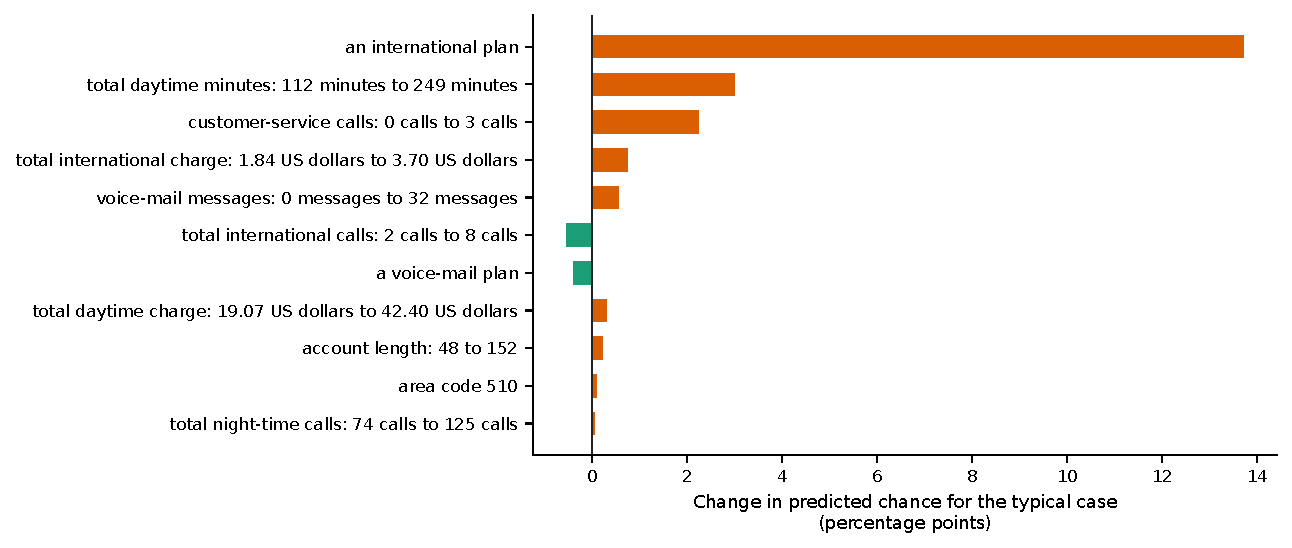
\includegraphics[width=\linewidth,height=0.88\textheight,keepaspectratio]{figures/churn100-s7-c1/ann_84-effects.pdf}
\caption{The whole model: Each input's change in the predicted value for the typical case across the whole model, largest first (orange: raises it, teal: lowers it).}
\label{fig:churn100s7c1:plot-ann84-0}
\end{figure}
\begin{figure}[H]\centering
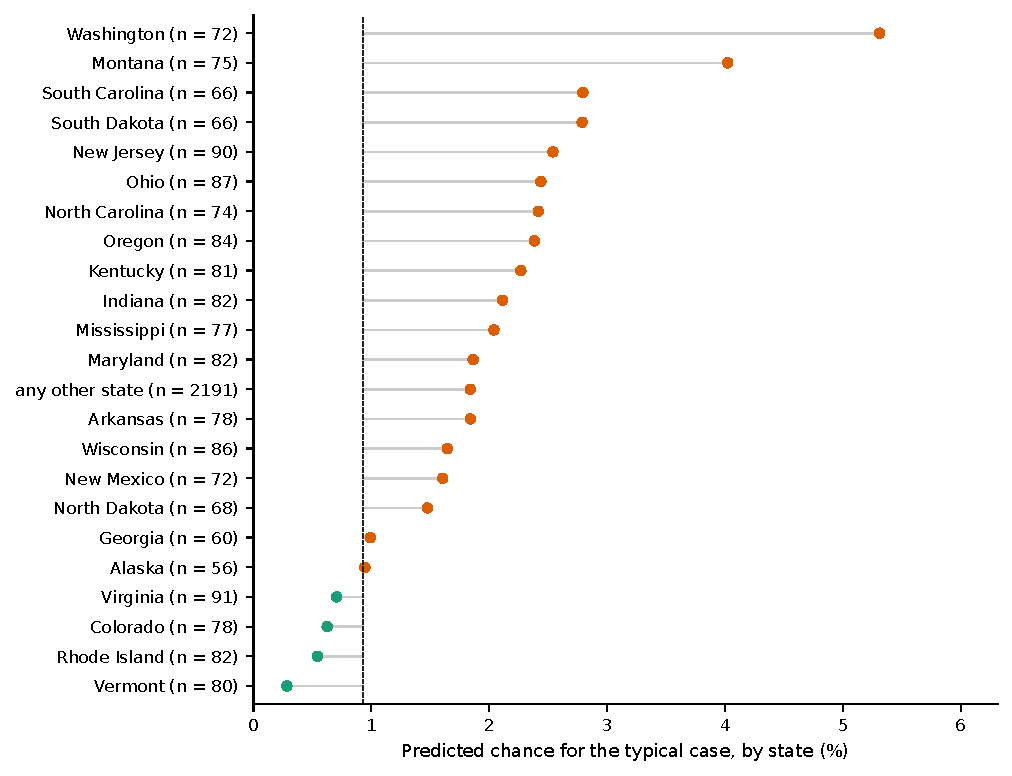
\includegraphics[width=\linewidth,height=0.88\textheight,keepaspectratio]{figures/churn100-s7-c1/ann_84-levels-state.pdf}
\caption{The whole model: Every level of state the model reads: the predicted value for the typical case at that level (dashed: the reference level); n = training customers; grey: few customers or not supported.}
\label{fig:churn100s7c1:plot-ann84-1}
\end{figure}
\par\smallskip\noindent{\small \textbf{Dive deeper:} Usage and service calls (\ref{rd:ann83}); International plan (\ref{rd:ann81}); Fixed-weight inputs (\ref{rd:ann78}); Voice mail and South Dakota (\ref{rd:ann80}); State adjustments (\ref{rd:ann82}). Technical detail: \ref{tech:ann84}.\par}
\subsubsection{Usage and service calls}\label{rd:ann83}
\noindent{\footnotesize Part of: The whole model (\ref{rd:ann84}).\par}
\noindent{\small Figure~\ref{fig:churn100s7c1:parts-ann83} shows what feeds this part; Figure~\ref{fig:churn100s7c1:units-ann83} its units and every connection into them (dashed boxes: connections from or to other parts, drawn in their own sections).\par}
\begin{figure}[H]\centering
\resizebox{!}{\ifdim\height>0.5\textheight 0.5\textheight\else\height\fi}{%
\resizebox{\ifdim\width>\linewidth\linewidth\else\width\fi}{!}{%
\begin{tikzpicture}[
  font=\sffamily\scriptsize, >={Stealth[length=1.6mm]},
  inp/.style={draw, rounded corners=1pt, fill=white, inner sep=1.5pt, minimum height=3.2mm, anchor=east},
  abox/.style={draw, thick, rounded corners=2pt, align=center, inner sep=3pt, minimum height=6mm, text width=42mm},
  outp/.style={draw, double, rounded corners=2pt, fill=white, align=center, inner sep=3pt, text width=24mm},
  agg/.style={draw=black!55},
]
\node[inp] (i0) at (0,2.25) {state};
\node[inp] (i1) at (0,1.5) {voice-mail plan};
\node[inp] (i2) at (0,0.75) {total daytime minutes};
\node[inp] (i3) at (0,-0.0) {total daytime charge};
\node[inp] (i4) at (0,-0.75) {total evening minutes};
\node[inp] (i5) at (0,-1.5) {total night-time minutes};
\node[inp] (i6) at (0,-2.25) {customer-service calls};
\node[abox, fill=RoyalBlue!18, draw=RoyalBlue!80!black] (b0) at (5.28,0.0) {\textbf{Usage score}};
\node[outp] (out) at (9.36,0) {Usage and service calls};
\begin{scope}[on background layer]
\draw[->, agg, thin] (i0.east) -- (b0.west);
\draw[->, agg, thin] (i1.east) -- (b0.west);
\draw[->, agg, thin] (i2.east) -- (b0.west);
\draw[->, agg, thin] (i3.east) -- (b0.west);
\draw[->, agg, thin] (i4.east) -- (b0.west);
\draw[->, agg, thin] (i5.east) -- (b0.west);
\draw[->, agg] (b0.east) -- (out.west);
\draw[->, agg, thin, dashed] (i6.east) -- (out.west);
\end{scope}
\end{tikzpicture}}}%
\caption{Usage and service calls: what feeds it, one level down.}
\label{fig:churn100s7c1:parts-ann83}
\end{figure}
\begin{figure}[H]\centering
\resizebox{\ifdim\width>\linewidth\linewidth\else\width\fi}{!}{%
\definecolor{netup}{HTML}{D95F02}\definecolor{netdown}{HTML}{1B9E77}\definecolor{netmixed}{HTML}{7F7F7F}%
\begin{tikzpicture}[
  font=\sffamily\scriptsize, >={Stealth[length=1.4mm]},
  inp/.style={draw, circle, fill=white, minimum size=3.2mm, inner sep=0pt},
  hid/.style={draw, circle, fill=white, minimum size=5.2mm, inner sep=0.5pt, font=\sffamily\tiny},
  exitbox/.style={draw, thick, rectangle, fill=white, align=center, text width=17mm, minimum height=5mm, inner sep=1.5pt, font=\sffamily\tiny},
  sumbox/.style={draw, thick, dashed, rectangle, fill=white, align=center, text width=17mm, minimum height=5mm, inner sep=1.5pt, font=\sffamily\tiny},
  outp/.style={draw, thick, regular polygon, regular polygon sides=6, fill=white, minimum size=10mm, inner sep=0pt, font=\sffamily\tiny, align=center},
  stub/.style={draw, dashed, rounded corners=2pt, fill=white, align=center, inner sep=2pt, font=\sffamily\tiny, text width=15mm},
  inlab/.style={font=\sffamily\tiny, align=center, text width=15mm, inner sep=1pt, fill=white, fill opacity=0.8, text opacity=1},
  wpos/.style={draw=NavyBlue}, wneg/.style={draw=BrickRed}, wagg/.style={draw=black!45, line width=1.2pt},
  wmix/.style={draw=Plum},
]
\node[hid] (n4344) at (3.05,1.9) {h5};
\node[hid] (n14351) at (1.55,1.9) {h14};
\node[exitbox] (nidentityxusage) at (2.3,4.6) {Usage and service calls $\uparrow$};
\node[hid] (n10552) at (2.3,3.25) {h10};
\node[inp, draw=netup, very thick] (ninxxnumberxcustomerxservicexcalls) at (3.2,0.0) {};
\path (ninxxnumberxcustomerxservicexcalls.south) node[inlab, anchor=north] (labninxxnumberxcustomerxservicexcalls) {customer-service calls $\uparrow$};
\node[stub] (nfromxxUsagexscore) at (1.4,0.0) {from Usage score};
\node[stub] (ntoxxthexmodelxoutput) at (2.3,6.15) {to the model output};
\begin{scope}[on background layer]
\node[fit=(n4344) (n14351) (nidentityxusage) (n10552) , inner sep=8pt, rounded corners=5pt, fill=BurntOrange!10, draw=BurntOrange!45] (clu0) {};
\draw[->, wpos, line width=0.51pt] (ninxxnumberxcustomerxservicexcalls) -- (n4344);
\draw[->, wneg, line width=1.38pt] (nfromxxUsagexscore) -- (n4344);
\draw[->, wpos, line width=0.63pt] (nfromxxUsagexscore) -- (n14351);
\draw[->, wpos, line width=0.66pt] (n14351) -- (n10552);
\draw[->, wpos, line width=1.15pt] (nfromxxUsagexscore) -- (nidentityxusage);
\draw[->, wpos, line width=1.26pt] (n4344) -- (nidentityxusage);
\draw[->, wpos, line width=1.32pt] (n10552) -- (nidentityxusage);
\draw[->, wpos, line width=0.60pt] (nidentityxusage) -- (ntoxxthexmodelxoutput);
\end{scope}
\node[font=\sffamily\scriptsize\bfseries, text=BurntOrange!55!black, anchor=south west, inner sep=1pt, fill=white, fill opacity=0.85, text opacity=1] at (clu0.north west) {Usage and service calls};
\end{tikzpicture}}%
\caption{Usage and service calls: its units and every connection into them. Blue: positive weight (raises the score); red: negative weight (lowers it); thicker: larger weight. Orange outline and up arrow: raises the final prediction; teal and down arrow: lowers it; grey and double arrow: depends.}
\label{fig:churn100s7c1:units-ann83}
\end{figure}
\paragraph{Hypothesis.} This part raises the chance of leaving for heavy daytime users without a voice-mail plan and for customers who call customer service 3 times or more: daytime minutes in an uneven way, and calls for most customers slowly at first, then faster, but for some customers without a voice-mail plan nothing until a point, then steadily.\,{\scriptsize\textcolor{NavyBlue}{[C056, C055]}}
\paragraph{Evidence.} It is made up of the usage score (explained below) together with customer-service calls, combined in a way that is not a simple sum.\,{\scriptsize\textcolor{NavyBlue}{[C060]}} Through it, daytime minutes add only above about 187 minutes for customers without a voice-mail plan, in an uneven way, from about 1\% to about 11\% between 0 and 271 minutes for a typical customer.\,{\scriptsize\textcolor{NavyBlue}{[C056]}} Customer-service calls add only from about 3 calls upwards, for most customers slowly at first, then faster, but for some customers without a voice-mail plan nothing until a point, then steadily, from about 1\% to about 15\% between 0 and 4 calls.\,{\scriptsize\textcolor{NavyBlue}{[C055]}}
\par\noindent{\small Evidence plots: Figure~\ref{fig:churn100s7c1:plot-ann83-0}, Figure~\ref{fig:churn100s7c1:plot-ann83-1}, Figure~\ref{fig:churn100s7c1:plot-ann83-2}, Figure~\ref{fig:churn100s7c1:plot-ann83-3}, Figure~\ref{fig:churn100s7c1:plot-ann83-4}, Figure~\ref{fig:churn100s7c1:plot-ann83-5}, Figure~\ref{fig:churn100s7c1:plot-ann83-6}.\par}
\par\noindent{\small Figure~\ref{fig:churn100s7c1:plot-ann83-5} shows this part's own output, unit h16: over its two main inputs, with the line where it switches on.\par}
\begin{figure}[H]\centering
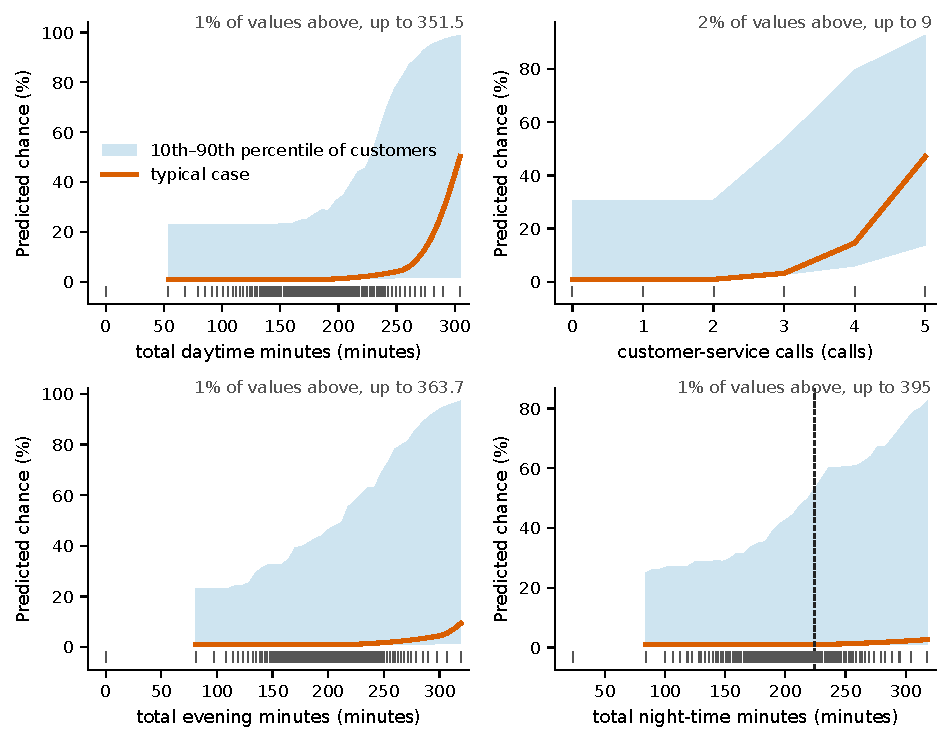
\includegraphics[width=\linewidth,height=0.88\textheight,keepaspectratio]{figures/churn100-s7-c1/ann_83-response.pdf}
\caption{Usage and service calls: Response curves through this part: the typical case (bold), the 10th to 90th percentile of individual customers (band), the fold or step point (dashed) with its spread across them (grey), and the observed values (ticks).}
\label{fig:churn100s7c1:plot-ann83-0}
\end{figure}
\begin{figure}[H]\centering
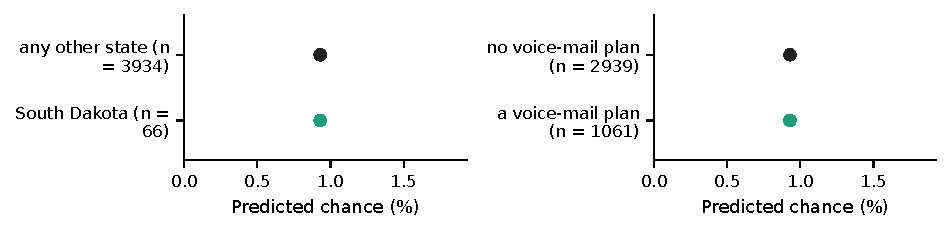
\includegraphics[width=\linewidth,height=0.88\textheight,keepaspectratio]{figures/churn100-s7-c1/ann_83-categories-small.pdf}
\caption{Usage and service calls: The predicted value for the typical case at each level, through this part (n = training customers; grey: fewer than 20).}
\label{fig:churn100s7c1:plot-ann83-1}
\end{figure}
\begin{figure}[H]\centering
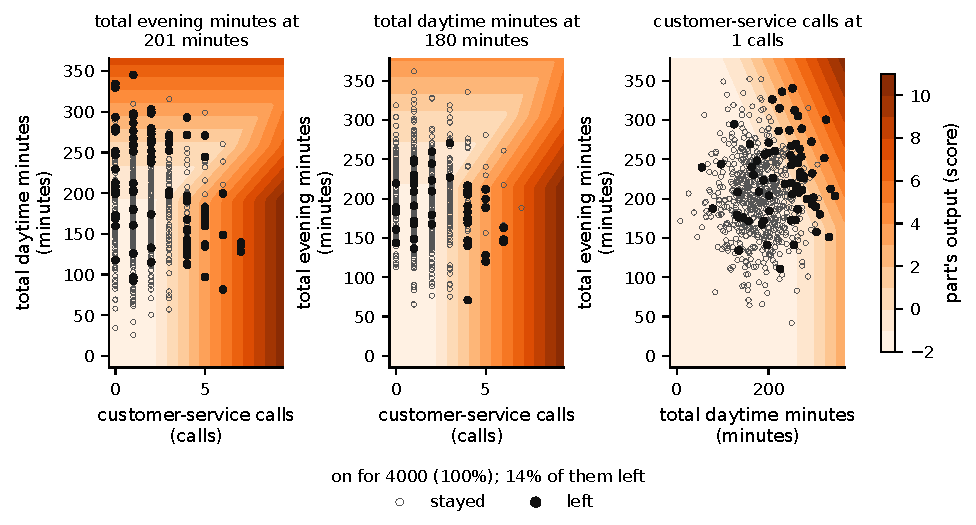
\includegraphics[width=\linewidth,height=0.88\textheight,keepaspectratio]{figures/churn100-s7-c1/ann_83-deep-map.pdf}
\caption{Usage and service calls: The part's own output over each pair of its three main inputs (the third held at its median, named above each panel; the points are the training rows whose third input is between its 40th and 60th percentile), other inputs at the typical case: colour where it is on, flat grey where it is switched off, the black line where it switches on; training customers as hollow (no event) and filled (event) points, so the part can be seen catching the events (the predicted-chance overlay was harder to read). The switch-on line is traced on this map only; the boundary claim (C118) did not pass its check on the data, so no rule is stated.}
\label{fig:churn100s7c1:plot-ann83-2}
\end{figure}
\begin{figure}[H]\centering
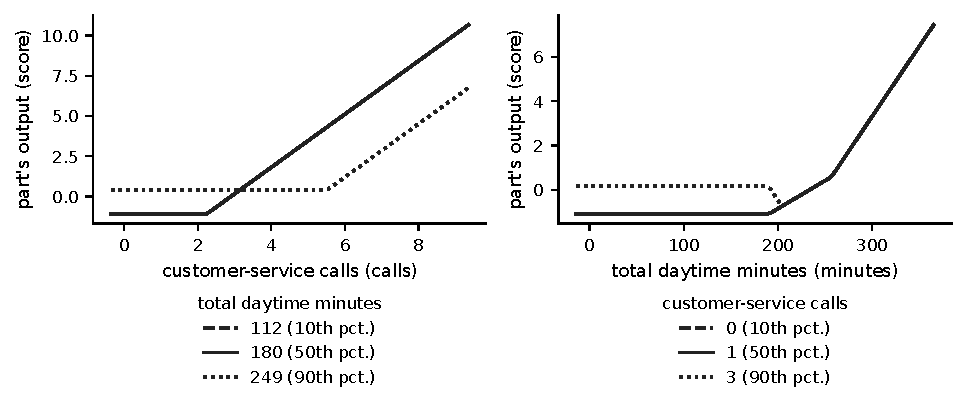
\includegraphics[width=\linewidth,height=0.88\textheight,keepaspectratio]{figures/churn100-s7-c1/ann_83-deep-slices.pdf}
\caption{Usage and service calls: Slices of the same map: the part's own output against each input at three values of the other, so the tilted boundary shows as a shifting hinge. The switch-on line is traced on this map only; the boundary claim (C118) did not pass its check on the data, so no rule is stated.}
\label{fig:churn100s7c1:plot-ann83-3}
\end{figure}
\begin{figure}[H]\centering
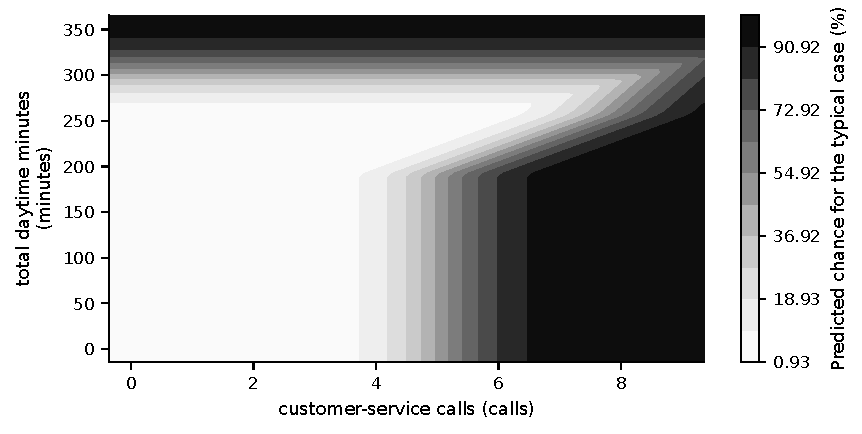
\includegraphics[width=\linewidth,height=0.88\textheight,keepaspectratio]{figures/churn100-s7-c1/ann_83-deep-risk.pdf}
\caption{Usage and service calls: The same map on the final scale: the predicted value for the typical case, with the switch-on line (orange). The switch-on line is traced on this map only; the boundary claim (C118) did not pass its check on the data, so no rule is stated.}
\label{fig:churn100s7c1:plot-ann83-4}
\end{figure}
\begin{figure}[H]\centering
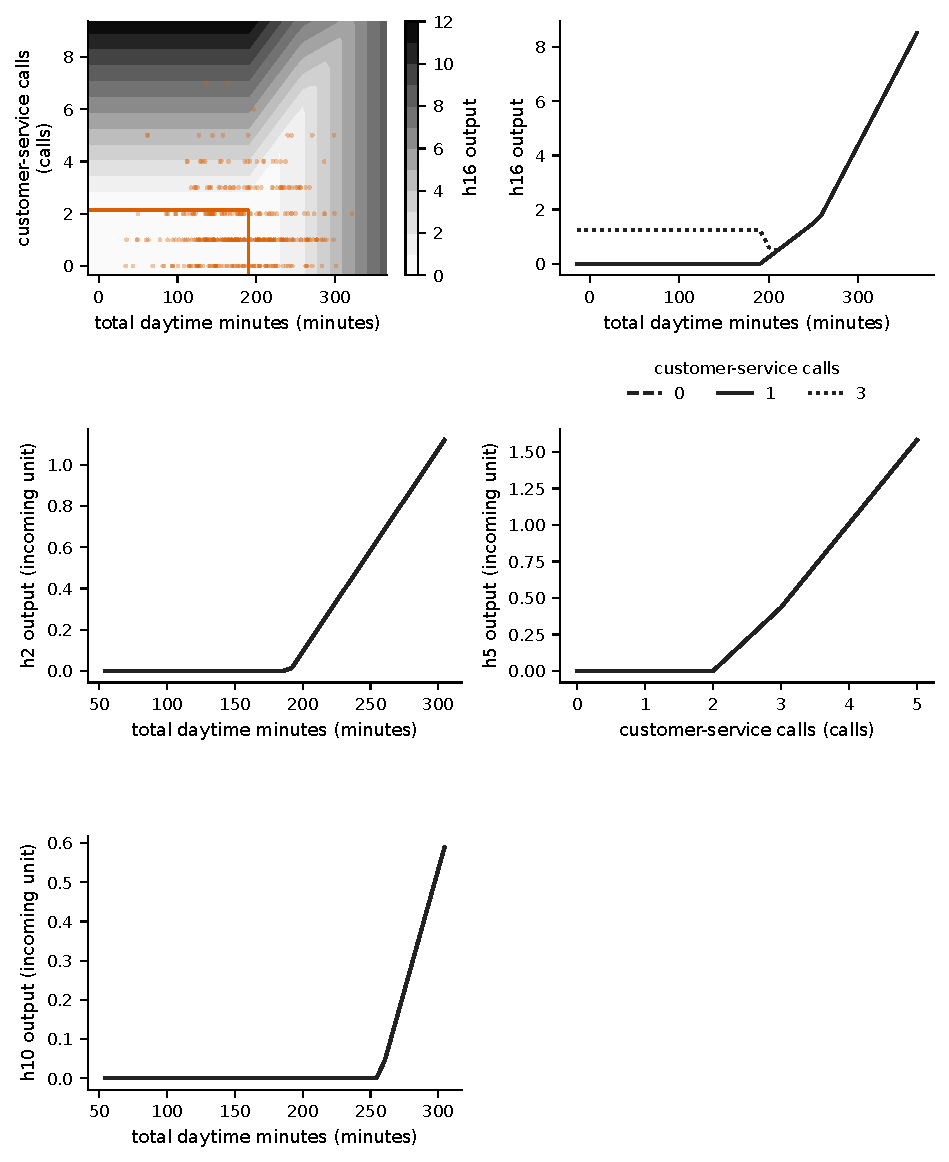
\includegraphics[width=\linewidth,height=0.88\textheight,keepaspectratio]{figures/churn100-s7-c1/ann_83-partial-identity_usage.pdf}
\caption{Usage and service calls: This part's own output, unit h16 (combines 3 non-linear units), on its own scale (its activation), with every other input at the typical case; it is active for 1927 of 4000. Left: its output over its two main inputs (orange line: where it switches on; dots: the data); right: slices at three values of the second input; then each incoming non-linear unit against its own main input.}
\label{fig:churn100s7c1:plot-ann83-5}
\end{figure}
\begin{figure}[H]\centering
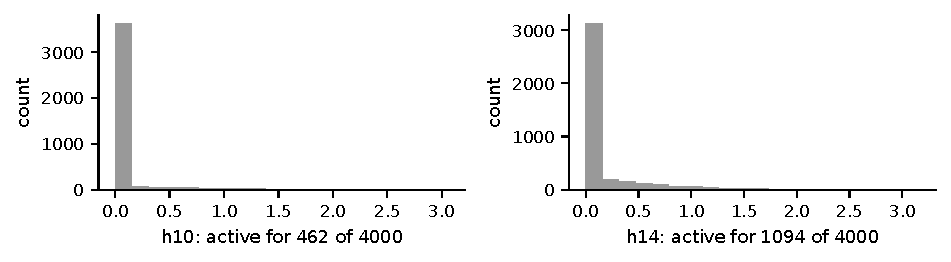
\includegraphics[width=\linewidth,height=0.88\textheight,keepaspectratio]{figures/churn100-s7-c1/ann_83-units.pdf}
\caption{Usage and service calls: This part's hidden units: each unit's output against its main numeric input (top) and how often it is active (bottom).}
\label{fig:churn100s7c1:plot-ann83-6}
\end{figure}
\par\smallskip\noindent{\small \textbf{Dive deeper:} Usage score (\ref{rd:ann79}). Technical detail: \ref{tech:ann83}.\par}
\subsubsection{Usage score}\label{rd:ann79}
\noindent{\footnotesize Part of: Usage and service calls (\ref{rd:ann83}).\par}
\noindent{\small Figure~\ref{fig:churn100s7c1:parts-ann79} shows what feeds this part; Figure~\ref{fig:churn100s7c1:units-ann79} its units and every connection into them (dashed boxes: connections from or to other parts, drawn in their own sections).\par}
\begin{figure}[H]\centering
\resizebox{!}{\ifdim\height>0.5\textheight 0.5\textheight\else\height\fi}{%
\resizebox{\ifdim\width>\linewidth\linewidth\else\width\fi}{!}{%
\begin{tikzpicture}[
  font=\sffamily\scriptsize, >={Stealth[length=1.6mm]},
  inp/.style={draw, rounded corners=1pt, fill=white, inner sep=1.5pt, minimum height=3.2mm, anchor=east},
  abox/.style={draw, thick, rounded corners=2pt, align=center, inner sep=3pt, minimum height=6mm, text width=42mm},
  outp/.style={draw, double, rounded corners=2pt, fill=white, align=center, inner sep=3pt, text width=24mm},
  agg/.style={draw=black!55},
]
\node[inp] (i0) at (0,1.875) {state};
\node[inp] (i1) at (0,1.125) {voice-mail plan};
\node[inp] (i2) at (0,0.375) {total daytime minutes};
\node[inp] (i3) at (0,-0.375) {total daytime charge};
\node[inp] (i4) at (0,-1.125) {total evening minutes};
\node[inp] (i5) at (0,-1.875) {total night-time minutes};
\node[outp] (out) at (9.36,0) {Usage score};
\begin{scope}[on background layer]
\draw[->, agg, thin, dashed] (i0.east) -- (out.west);
\draw[->, agg, thin, dashed] (i1.east) -- (out.west);
\draw[->, agg, thin, dashed] (i2.east) -- (out.west);
\draw[->, agg, thin, dashed] (i3.east) -- (out.west);
\draw[->, agg, thin, dashed] (i4.east) -- (out.west);
\draw[->, agg, thin, dashed] (i5.east) -- (out.west);
\end{scope}
\end{tikzpicture}}}%
\caption{Usage score: what feeds it, one level down.}
\label{fig:churn100s7c1:parts-ann79}
\end{figure}
\begin{figure}[H]\centering
\resizebox{\ifdim\width>\linewidth\linewidth\else\width\fi}{!}{%
\definecolor{netup}{HTML}{D95F02}\definecolor{netdown}{HTML}{1B9E77}\definecolor{netmixed}{HTML}{7F7F7F}%
\begin{tikzpicture}[
  font=\sffamily\scriptsize, >={Stealth[length=1.4mm]},
  inp/.style={draw, circle, fill=white, minimum size=3.2mm, inner sep=0pt},
  hid/.style={draw, circle, fill=white, minimum size=5.2mm, inner sep=0.5pt, font=\sffamily\tiny},
  exitbox/.style={draw, thick, rectangle, fill=white, align=center, text width=17mm, minimum height=5mm, inner sep=1.5pt, font=\sffamily\tiny},
  sumbox/.style={draw, thick, dashed, rectangle, fill=white, align=center, text width=17mm, minimum height=5mm, inner sep=1.5pt, font=\sffamily\tiny},
  outp/.style={draw, thick, regular polygon, regular polygon sides=6, fill=white, minimum size=10mm, inner sep=0pt, font=\sffamily\tiny, align=center},
  stub/.style={draw, dashed, rounded corners=2pt, fill=white, align=center, inner sep=2pt, font=\sffamily\tiny, text width=15mm},
  inlab/.style={font=\sffamily\tiny, align=center, text width=15mm, inner sep=1pt, fill=white, fill opacity=0.8, text opacity=1},
  wpos/.style={draw=NavyBlue}, wneg/.style={draw=BrickRed}, wagg/.style={draw=black!45, line width=1.2pt},
  wmix/.style={draw=Plum},
]
\node[hid] (n7558) at (5.4,3.25) {h9};
\node[exitbox] (n879) at (5.4,4.6) {Usage score $\updownarrow$};
\node[hid] (n1406) at (5.4,1.9) {h3};
\node[inp, draw=netup, very thick] (ninxxtotalxdayxminutes) at (6.3,0.0) {};
\path (ninxxtotalxdayxminutes.south) node[inlab, anchor=north] (labninxxtotalxdayxminutes) {total daytime minutes $\uparrow$};
\node[inp, draw=netup, very thick] (ninxxtotalxdayxcharge) at (4.5,0.0) {};
\path (ninxxtotalxdayxcharge.south) node[inlab, anchor=north] (labninxxtotalxdayxcharge) {total daytime charge $\uparrow$};
\node[inp, draw=netmixed, very thick] (ngrpxxstate) at (2.7,0.0) {};
\path (ngrpxxstate.south) node[inlab, anchor=north] (labngrpxxstate) {state (23 of 51 used) $\updownarrow$};
\node[inp, draw=netdown, very thick] (ninxxvoicexmailxplan) at (0.9,0.0) {};
\path (ninxxvoicexmailxplan.south) node[inlab, anchor=north] (labninxxvoicexmailxplan) {a voice-mail plan $\downarrow$};
\node[inp, draw=netup, very thick] (ninxxtotalxevexminutes) at (8.1,0.0) {};
\path (ninxxtotalxevexminutes.south) node[inlab, anchor=north] (labninxxtotalxevexminutes) {total evening minutes $\uparrow$};
\node[inp, draw=netup, very thick] (ninxxtotalxnightxminutes) at (9.9,0.0) {};
\path (ninxxtotalxnightxminutes.south) node[inlab, anchor=north] (labninxxtotalxnightxminutes) {total night-time minutes $\uparrow$};
\node[stub] (ntoxxUsagexandxservicexcalls) at (5.4,6.15) {to Usage and service calls};
\begin{scope}[on background layer]
\node[fit=(n7558) (n879) (n1406) , inner sep=8pt, rounded corners=5pt, fill=BurntOrange!10, draw=BurntOrange!45] (clu0) {};
\draw[->, wpos, line width=0.43pt] (ninxxtotalxdayxminutes) -- (n879);
\draw[->, wpos, line width=0.44pt] (ninxxtotalxdayxcharge) -- (n1406);
\draw[->, wpos, line width=0.44pt] (n7558) -- (n879);
\draw[->, wpos, line width=0.67pt] (n1406) -- (n7558);
\draw[->, wneg, line width=0.60pt] (ninxxvoicexmailxplan) -- (n879);
\draw[->, wpos, line width=0.48pt] (ninxxtotalxevexminutes) -- (n7558);
\draw[->, wpos, line width=0.33pt] (ninxxtotalxnightxminutes) -- (n879);
\draw[->, wneg, line width=1.38pt] (n879) -- (ntoxxUsagexandxservicexcalls);
\draw[->, wpos, line width=0.63pt] (n879) -- (ntoxxUsagexandxservicexcalls);
\draw[->, wpos, line width=1.15pt] (n879) -- (ntoxxUsagexandxservicexcalls);
\draw[->, wneg, line width=0.56pt] (ngrpxxstate) -- node[pos=0.8, sloped, above, font=\sffamily\tiny, inner sep=1pt, fill=white, fill opacity=0.8, text opacity=1] {-0.88} (n1406);
\end{scope}
\node[font=\sffamily\scriptsize\bfseries, text=BurntOrange!55!black, anchor=south west, inner sep=1pt, fill=white, fill opacity=0.85, text opacity=1] at (clu0.north west) {Usage score};
\end{tikzpicture}}%
\caption{Usage score: its units and every connection into them. Blue: positive weight (raises the score); red: negative weight (lowers it); thicker: larger weight. Orange outline and up arrow: raises the final prediction; teal and down arrow: lowers it; grey and double arrow: depends.}
\label{fig:churn100s7c1:units-ann79}
\end{figure}
\paragraph{Hypothesis.} This part builds a usage score: heavy daytime use raises the chance of leaving, in an uneven way and more so with high evening minutes, and a voice-mail plan lowers it.\,{\scriptsize\textcolor{NavyBlue}{[C071, C067, C062]}}
\paragraph{Evidence.} Through it, daytime minutes add only above about 187 minutes for customers without a voice-mail plan, in an uneven way, from about 1\% to about 11\% between 0 and 271 minutes.\,{\scriptsize\textcolor{NavyBlue}{[C071]}} Daytime minutes count more with more than 201 evening minutes (about 1\% to about 11\%, against about 1\% to about 2\%) and with more than 200 night-time minutes (about 1\% to about 7\%, against about 1\% to about 3\%), in an uneven way.\,{\scriptsize\textcolor{NavyBlue}{[C067, C068]}} A voice-mail plan lowers the chance through it from about 3\% to about 1\% for the typical customer it acts on.\,{\scriptsize\textcolor{NavyBlue}{[C062]}} Its formula reproduces the part exactly on all 4000 training customers.\,{\scriptsize\textcolor{NavyBlue}{[C076]}}
\par\noindent{\small Evidence plots: Figure~\ref{fig:churn100s7c1:plot-ann79-0}, Figure~\ref{fig:churn100s7c1:plot-ann79-1}, Figure~\ref{fig:churn100s7c1:plot-ann79-2}, Figure~\ref{fig:churn100s7c1:plot-ann79-3}, Figure~\ref{fig:churn100s7c1:plot-ann79-4}, Figure~\ref{fig:churn100s7c1:plot-ann79-5}, Figure~\ref{fig:churn100s7c1:plot-ann79-6}, Figure~\ref{fig:churn100s7c1:plot-ann79-7}.\par}
\par\medskip\noindent\textbf{Worked example: reading this part.} Figure~\ref{fig:churn100s7c1:plot-ann79-3} maps the part's own output over its main inputs. In the grey region it is switched off and adds nothing; past the black line it switches on, and the colour shows how much it adds to the score. The line is the rule in the claim (C119): it switches on when total daytime minutes above about 220 (for total evening minutes from about 0.00 to 164); total daytime minutes plus about 0.75 $\times$ total evening minutes above about 341 (for total evening minutes from about 164 to 364). 1382 of 4000 training customers lie on the 'on' side, and 23\% of them left, against 10\% of the others: the filled points crowd on the 'on' side. Figure~\ref{fig:churn100s7c1:plot-ann79-4} cuts the map into slices: the hinge moves as the other input changes, which is what a tilted line means. Figure~\ref{fig:churn100s7c1:plot-ann79-5} shows what this does to the final prediction for the typical case.\par
\par\noindent{\small Figure~\ref{fig:churn100s7c1:plot-ann79-6} shows this part's own output, unit h2: over its two main inputs, with the line where it switches on.\par}
\begin{figure}[H]\centering
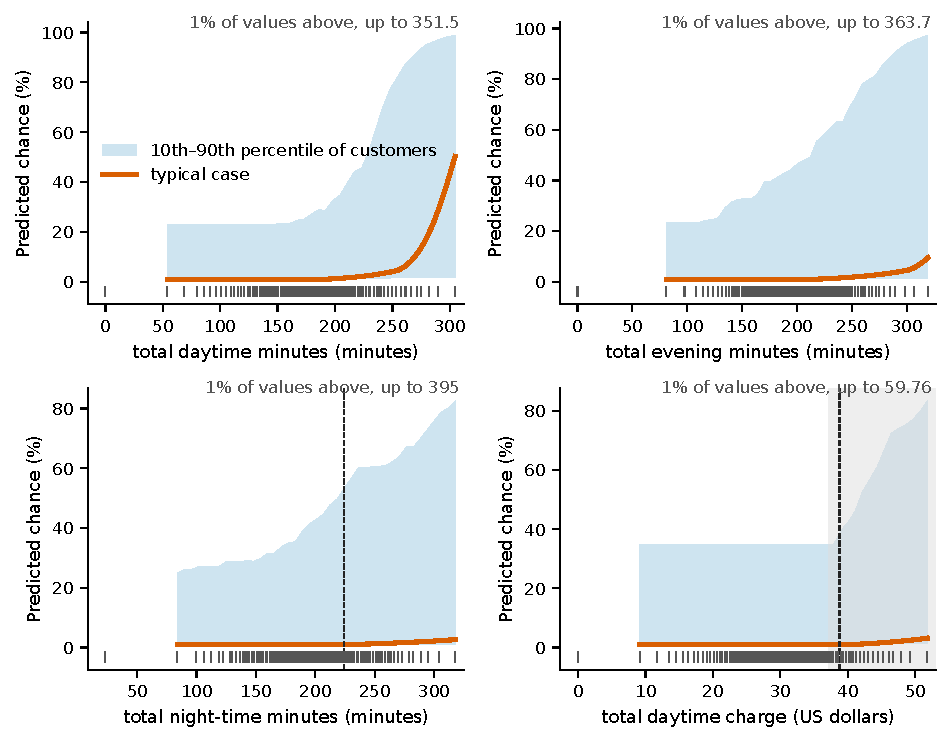
\includegraphics[width=\linewidth,height=0.88\textheight,keepaspectratio]{figures/churn100-s7-c1/ann_79-response.pdf}
\caption{Usage score: Response curves through this part: the typical case (bold), the 10th to 90th percentile of individual customers (band), the fold or step point (dashed) with its spread across them (grey), and the observed values (ticks).}
\label{fig:churn100s7c1:plot-ann79-0}
\end{figure}
\begin{figure}[H]\centering
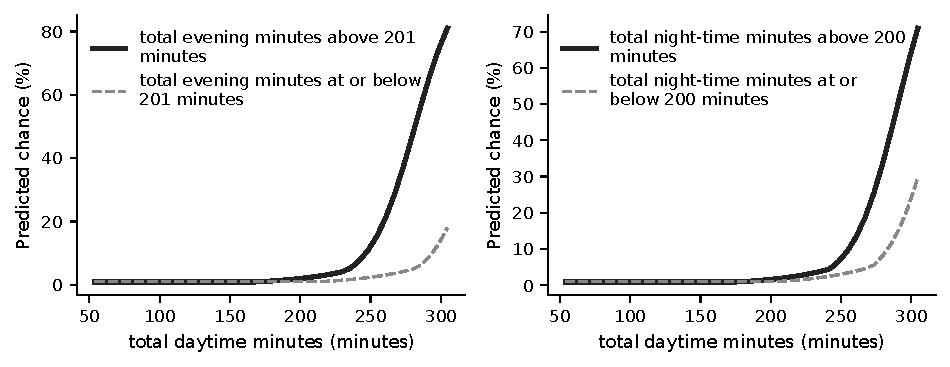
\includegraphics[width=\linewidth,height=0.88\textheight,keepaspectratio]{figures/churn100-s7-c1/ann_79-interaction.pdf}
\caption{Usage score: How the effect differs between groups: one curve per group, for the typical case of each group.}
\label{fig:churn100s7c1:plot-ann79-1}
\end{figure}
\begin{figure}[H]\centering
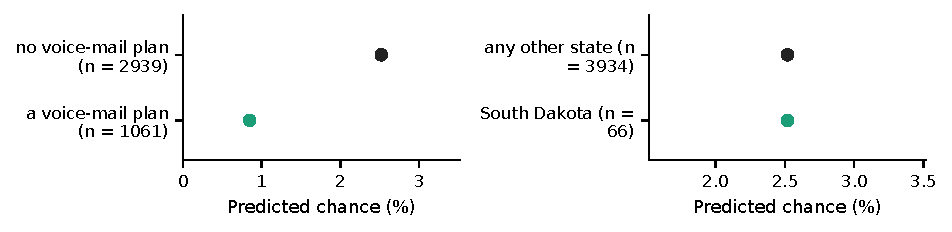
\includegraphics[width=\linewidth,height=0.88\textheight,keepaspectratio]{figures/churn100-s7-c1/ann_79-categories-small.pdf}
\caption{Usage score: The predicted value for the typical case at each level, through this part (n = training customers; grey: fewer than 20).}
\label{fig:churn100s7c1:plot-ann79-2}
\end{figure}
\begin{figure}[H]\centering
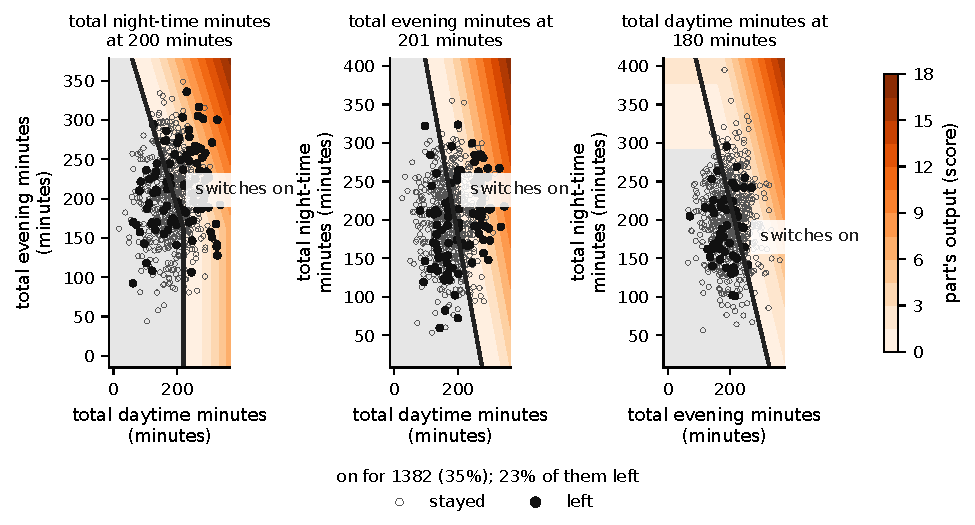
\includegraphics[width=\linewidth,height=0.88\textheight,keepaspectratio]{figures/churn100-s7-c1/ann_79-deep-map.pdf}
\caption{Usage score: The part's own output over each pair of its three main inputs (the third held at its median, named above each panel; the points are the training rows whose third input is between its 40th and 60th percentile), other inputs at the typical case: colour where it is on, flat grey where it is switched off, the black line where it switches on; training customers as hollow (no event) and filled (event) points, so the part can be seen catching the events (the predicted-chance overlay was harder to read).}
\label{fig:churn100s7c1:plot-ann79-3}
\end{figure}
\begin{figure}[H]\centering
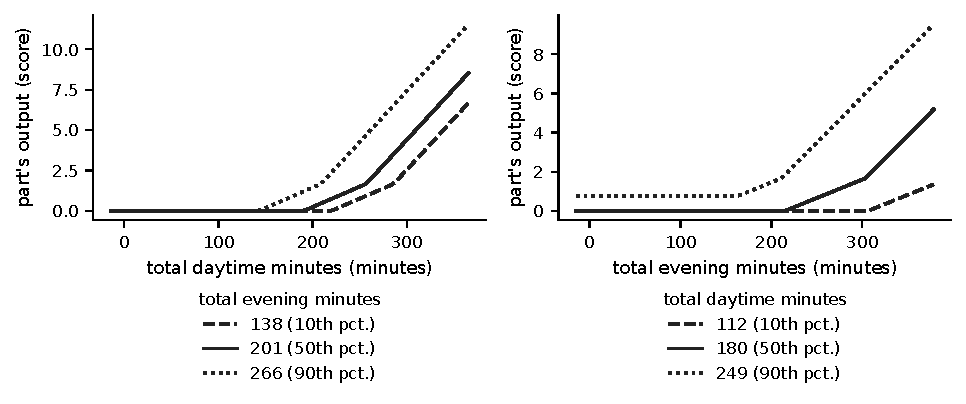
\includegraphics[width=\linewidth,height=0.88\textheight,keepaspectratio]{figures/churn100-s7-c1/ann_79-deep-slices.pdf}
\caption{Usage score: Slices of the same map: the part's own output against each input at three values of the other, so the tilted boundary shows as a shifting hinge.}
\label{fig:churn100s7c1:plot-ann79-4}
\end{figure}
\begin{figure}[H]\centering
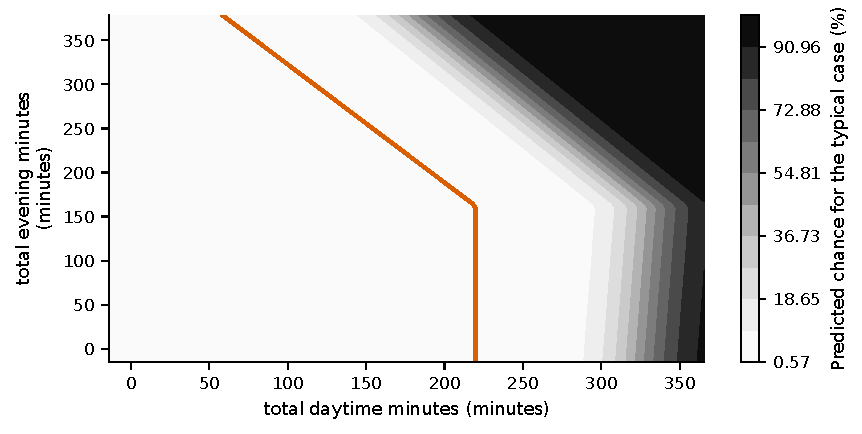
\includegraphics[width=\linewidth,height=0.88\textheight,keepaspectratio]{figures/churn100-s7-c1/ann_79-deep-risk.pdf}
\caption{Usage score: The same map on the final scale: the predicted value for the typical case, with the switch-on line (orange).}
\label{fig:churn100s7c1:plot-ann79-5}
\end{figure}
\begin{figure}[H]\centering
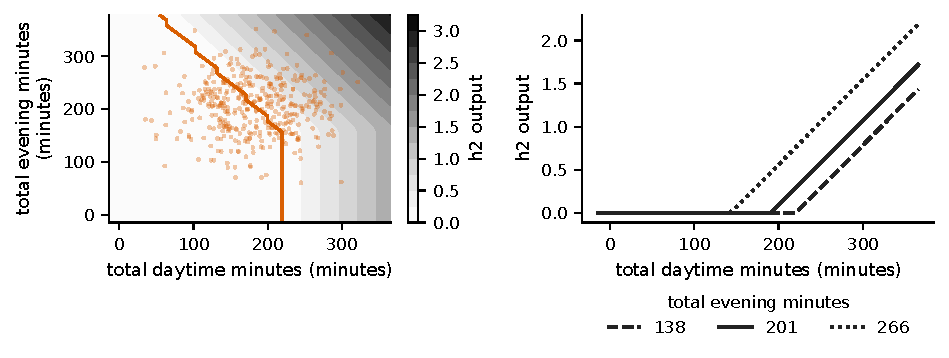
\includegraphics[width=\linewidth,height=0.88\textheight,keepaspectratio]{figures/churn100-s7-c1/ann_79-partial-879.pdf}
\caption{Usage score: This part's own output, unit h2 (the output of 'Usage score'), on its own scale (its activation), with every other input at the typical case; it is active for 1382 of 4000. Left: its output over its two main inputs (orange line: where it switches on; dots: the data); right: slices at three values of the second input.}
\label{fig:churn100s7c1:plot-ann79-6}
\end{figure}
\begin{figure}[H]\centering
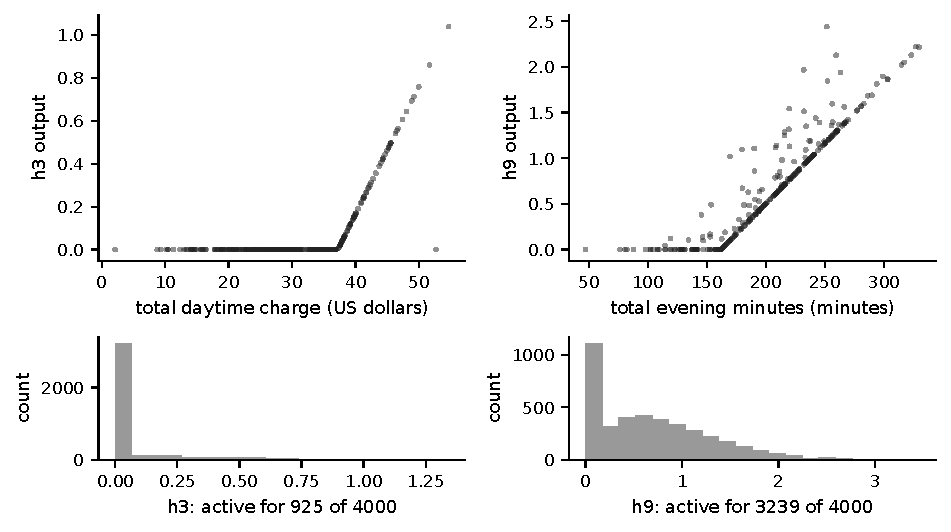
\includegraphics[width=\linewidth,height=0.88\textheight,keepaspectratio]{figures/churn100-s7-c1/ann_79-units.pdf}
\caption{Usage score: This part's hidden units: each unit's output against its main numeric input (top) and how often it is active (bottom).}
\label{fig:churn100s7c1:plot-ann79-7}
\end{figure}
\par\smallskip\noindent{\small Technical detail: \ref{tech:ann79}.\par}
\subsubsection{International plan}\label{rd:ann81}
\noindent{\footnotesize Part of: The whole model (\ref{rd:ann84}).\par}
\noindent{\small Figure~\ref{fig:churn100s7c1:parts-ann81} shows what feeds this part; Figure~\ref{fig:churn100s7c1:units-ann81} its units and every connection into them (dashed boxes: connections from or to other parts, drawn in their own sections).\par}
\begin{figure}[H]\centering
\resizebox{!}{\ifdim\height>0.5\textheight 0.5\textheight\else\height\fi}{%
\resizebox{\ifdim\width>\linewidth\linewidth\else\width\fi}{!}{%
\begin{tikzpicture}[
  font=\sffamily\scriptsize, >={Stealth[length=1.6mm]},
  inp/.style={draw, rounded corners=1pt, fill=white, inner sep=1.5pt, minimum height=3.2mm, anchor=east},
  abox/.style={draw, thick, rounded corners=2pt, align=center, inner sep=3pt, minimum height=6mm, text width=42mm},
  outp/.style={draw, double, rounded corners=2pt, fill=white, align=center, inner sep=3pt, text width=24mm},
  agg/.style={draw=black!55},
]
\node[inp] (i0) at (0,-0.0) {international calling plan};
\node[outp] (out) at (9.36,0) {International plan};
\begin{scope}[on background layer]
\draw[->, agg, thin, dashed] (i0.east) -- (out.west);
\end{scope}
\end{tikzpicture}}}%
\caption{International plan: what feeds it, one level down.}
\label{fig:churn100s7c1:parts-ann81}
\end{figure}
\begin{figure}[H]\centering
\resizebox{\ifdim\width>\linewidth\linewidth\else\width\fi}{!}{%
\definecolor{netup}{HTML}{D95F02}\definecolor{netdown}{HTML}{1B9E77}\definecolor{netmixed}{HTML}{7F7F7F}%
\begin{tikzpicture}[
  font=\sffamily\scriptsize, >={Stealth[length=1.4mm]},
  inp/.style={draw, circle, fill=white, minimum size=3.2mm, inner sep=0pt},
  hid/.style={draw, circle, fill=white, minimum size=5.2mm, inner sep=0.5pt, font=\sffamily\tiny},
  exitbox/.style={draw, thick, rectangle, fill=white, align=center, text width=17mm, minimum height=5mm, inner sep=1.5pt, font=\sffamily\tiny},
  sumbox/.style={draw, thick, dashed, rectangle, fill=white, align=center, text width=17mm, minimum height=5mm, inner sep=1.5pt, font=\sffamily\tiny},
  outp/.style={draw, thick, regular polygon, regular polygon sides=6, fill=white, minimum size=10mm, inner sep=0pt, font=\sffamily\tiny, align=center},
  stub/.style={draw, dashed, rounded corners=2pt, fill=white, align=center, inner sep=2pt, font=\sffamily\tiny, text width=15mm},
  inlab/.style={font=\sffamily\tiny, align=center, text width=15mm, inner sep=1pt, fill=white, fill opacity=0.8, text opacity=1},
  wpos/.style={draw=NavyBlue}, wneg/.style={draw=BrickRed}, wagg/.style={draw=black!45, line width=1.2pt},
  wmix/.style={draw=Plum},
]
\node[exitbox] (n6711) at (1.8,1.9) {International plan $\uparrow$};
\node[inp, draw=netup, very thick] (ninxxinternationalxplan) at (1.8,0.0) {};
\path (ninxxinternationalxplan.south) node[inlab, anchor=north] (labninxxinternationalxplan) {an international plan $\uparrow$};
\node[stub] (ntoxxthexmodelxoutput) at (1.8,3.45) {to the model output};
\begin{scope}[on background layer]
\node[fit=(n6711) , inner sep=8pt, rounded corners=5pt, fill=ForestGreen!10, draw=ForestGreen!45] (clu0) {};
\draw[->, wpos, line width=0.47pt] (ninxxinternationalxplan) -- (n6711);
\draw[->, wpos, line width=0.84pt] (n6711) -- (ntoxxthexmodelxoutput);
\end{scope}
\node[font=\sffamily\scriptsize\bfseries, text=ForestGreen!55!black, anchor=south west, inner sep=1pt, fill=white, fill opacity=0.85, text opacity=1] at (clu0.north west) {International plan};
\end{tikzpicture}}%
\caption{International plan: its units and every connection into them. Blue: positive weight (raises the score); red: negative weight (lowers it); thicker: larger weight. Orange outline and up arrow: raises the final prediction; teal and down arrow: lowers it; grey and double arrow: depends.}
\label{fig:churn100s7c1:units-ann81}
\end{figure}
\paragraph{Hypothesis.} This part raises the chance of leaving for customers with an international plan.\,{\scriptsize\textcolor{NavyBlue}{[C077]}}
\paragraph{Evidence.} It acts on the 380 of 4000 training customers with an international plan, 161 of whom left; for the typical customer it acts on, the chance is about 2\% without it and about 26\% with it.\,{\scriptsize\textcolor{NavyBlue}{[C078]}} For a typical customer, an international plan takes the chance from about 1\% to about 15\%.\,{\scriptsize\textcolor{NavyBlue}{[C077]}} Its formula reproduces the part exactly on all 4000 training customers.\,{\scriptsize\textcolor{NavyBlue}{[C079]}}
\par\noindent{\small Evidence plots: Figure~\ref{fig:churn100s7c1:plot-ann81-0}, Figure~\ref{fig:churn100s7c1:plot-ann81-1}.\par}
\begin{figure}[H]\centering
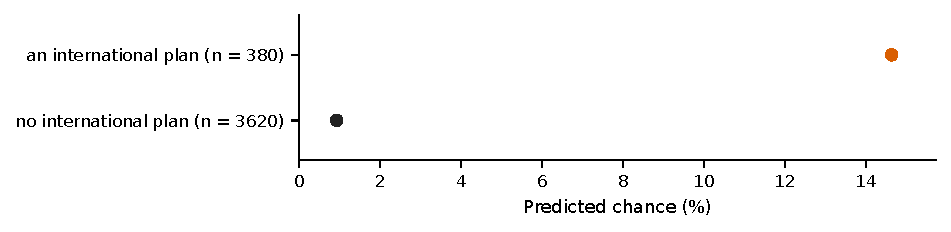
\includegraphics[width=\linewidth,height=0.88\textheight,keepaspectratio]{figures/churn100-s7-c1/ann_81-categories-small.pdf}
\caption{International plan: The predicted value for the typical case at each level, through this part (n = training customers; grey: fewer than 20).}
\label{fig:churn100s7c1:plot-ann81-0}
\end{figure}
\begin{figure}[H]\centering
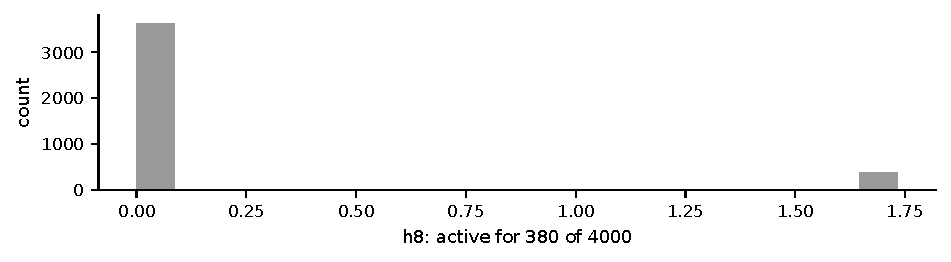
\includegraphics[width=\linewidth,height=0.88\textheight,keepaspectratio]{figures/churn100-s7-c1/ann_81-units.pdf}
\caption{International plan: This part's hidden units: each unit's output against its main numeric input (top) and how often it is active (bottom).}
\label{fig:churn100s7c1:plot-ann81-1}
\end{figure}
\par\smallskip\noindent{\small Technical detail: \ref{tech:ann81}.\par}
\subsubsection{Fixed-weight inputs}\label{rd:ann78}
\noindent{\footnotesize Part of: The whole model (\ref{rd:ann84}).\par}
\noindent{\small Figure~\ref{fig:churn100s7c1:parts-ann78} shows what feeds this part; Figure~\ref{fig:churn100s7c1:units-ann78} its units and every connection into them (dashed boxes: connections from or to other parts, drawn in their own sections).\par}
\begin{figure}[H]\centering
\resizebox{!}{\ifdim\height>0.5\textheight 0.5\textheight\else\height\fi}{%
\resizebox{\ifdim\width>\linewidth\linewidth\else\width\fi}{!}{%
\begin{tikzpicture}[
  font=\sffamily\scriptsize, >={Stealth[length=1.6mm]},
  inp/.style={draw, rounded corners=1pt, fill=white, inner sep=1.5pt, minimum height=3.2mm, anchor=east},
  abox/.style={draw, thick, rounded corners=2pt, align=center, inner sep=3pt, minimum height=6mm, text width=42mm},
  outp/.style={draw, double, rounded corners=2pt, fill=white, align=center, inner sep=3pt, text width=24mm},
  agg/.style={draw=black!55},
]
\node[inp] (i0) at (0,3.0) {state};
\node[inp] (i1) at (0,2.25) {account length};
\node[inp] (i2) at (0,1.5) {area code};
\node[inp] (i3) at (0,0.75) {voice-mail messages};
\node[inp] (i4) at (0,-0.0) {total evening minutes};
\node[inp] (i5) at (0,-0.75) {total night-time minutes};
\node[inp] (i6) at (0,-1.5) {total night-time calls};
\node[inp] (i7) at (0,-2.25) {total international calls};
\node[inp] (i8) at (0,-3.0) {total international charge};
\node[outp] (out) at (9.36,0) {Fixed-weight inputs};
\begin{scope}[on background layer]
\draw[->, agg, thin, dashed] (i0.east) -- (out.west);
\draw[->, agg, thin, dashed] (i1.east) -- (out.west);
\draw[->, agg, thin, dashed] (i2.east) -- (out.west);
\draw[->, agg, thin, dashed] (i3.east) -- (out.west);
\draw[->, agg, thin, dashed] (i4.east) -- (out.west);
\draw[->, agg, thin, dashed] (i5.east) -- (out.west);
\draw[->, agg, thin, dashed] (i6.east) -- (out.west);
\draw[->, agg, thin, dashed] (i7.east) -- (out.west);
\draw[->, agg, thin, dashed] (i8.east) -- (out.west);
\end{scope}
\end{tikzpicture}}}%
\caption{Fixed-weight inputs: what feeds it, one level down.}
\label{fig:churn100s7c1:parts-ann78}
\end{figure}
\begin{figure}[H]\centering
\resizebox{\ifdim\width>\linewidth\linewidth\else\width\fi}{!}{%
\definecolor{netup}{HTML}{D95F02}\definecolor{netdown}{HTML}{1B9E77}\definecolor{netmixed}{HTML}{7F7F7F}%
\begin{tikzpicture}[
  font=\sffamily\scriptsize, >={Stealth[length=1.4mm]},
  inp/.style={draw, circle, fill=white, minimum size=3.2mm, inner sep=0pt},
  hid/.style={draw, circle, fill=white, minimum size=5.2mm, inner sep=0.5pt, font=\sffamily\tiny},
  exitbox/.style={draw, thick, rectangle, fill=white, align=center, text width=17mm, minimum height=5mm, inner sep=1.5pt, font=\sffamily\tiny},
  sumbox/.style={draw, thick, dashed, rectangle, fill=white, align=center, text width=17mm, minimum height=5mm, inner sep=1.5pt, font=\sffamily\tiny},
  outp/.style={draw, thick, regular polygon, regular polygon sides=6, fill=white, minimum size=10mm, inner sep=0pt, font=\sffamily\tiny, align=center},
  stub/.style={draw, dashed, rounded corners=2pt, fill=white, align=center, inner sep=2pt, font=\sffamily\tiny, text width=15mm},
  inlab/.style={font=\sffamily\tiny, align=center, text width=15mm, inner sep=1pt, fill=white, fill opacity=0.8, text opacity=1},
  wpos/.style={draw=NavyBlue}, wneg/.style={draw=BrickRed}, wagg/.style={draw=black!45, line width=1.2pt},
  wmix/.style={draw=Plum},
]
\node[exitbox] (nidentityxlin) at (5.85,1.9) {Fixed-weight inputs $\uparrow$};
\node[inp, draw=netmixed, very thick] (ngrpxxstate) at (2.7,0.0) {};
\path (ngrpxxstate.south) node[inlab, anchor=north] (labngrpxxstate) {state (23 of 51 used) $\updownarrow$};
\node[inp, draw=netup, very thick] (ninxxaccountxlength) at (0.9,0.0) {};
\path (ninxxaccountxlength.south) node[inlab, anchor=north] (labninxxaccountxlength) {account length $\uparrow$};
\node[inp, draw=netup, very thick] (ninxxareaxcodex510) at (1.8,-1.05) {};
\path (ninxxareaxcodex510.south) node[inlab, anchor=north] (labninxxareaxcodex510) {area code 510 $\uparrow$};
\node[inp, draw=netup, very thick] (ninxxnumberxvmailxmessages) at (9.9,0.0) {};
\path (ninxxnumberxvmailxmessages.south) node[inlab, anchor=north] (labninxxnumberxvmailxmessages) {voice-mail messages $\uparrow$};
\node[inp, draw=netup, very thick] (ninxxtotalxnightxcalls) at (6.3,0.0) {};
\path (ninxxtotalxnightxcalls.south) node[inlab, anchor=north] (labninxxtotalxnightxcalls) {total night-time calls $\uparrow$};
\node[inp, draw=netdown, very thick] (ninxxtotalxintlxcalls) at (4.5,0.0) {};
\path (ninxxtotalxintlxcalls.south) node[inlab, anchor=north] (labninxxtotalxintlxcalls) {total international calls $\downarrow$};
\node[inp, draw=netup, very thick] (ninxxtotalxintlxcharge) at (5.4,-1.05) {};
\path (ninxxtotalxintlxcharge.south) node[inlab, anchor=north] (labninxxtotalxintlxcharge) {total international charge $\uparrow$};
\node[inp, draw=netdown, very thick] (ninxxtotalxevexminutes) at (3.6,-1.05) {};
\path (ninxxtotalxevexminutes.south) node[inlab, anchor=north] (labninxxtotalxevexminutes) {total evening minutes $\downarrow$};
\node[inp, draw=netdown, very thick] (ninxxtotalxnightxminutes) at (8.1,0.0) {};
\path (ninxxtotalxnightxminutes.south) node[inlab, anchor=north] (labninxxtotalxnightxminutes) {total night-time minutes $\downarrow$};
\node[stub] (ntoxxthexmodelxoutput) at (5.4,3.45) {to the model output};
\begin{scope}[on background layer]
\node[fit=(nidentityxlin) , inner sep=8pt, rounded corners=5pt, fill=Orchid!10, draw=Orchid!45] (clu0) {};
\draw[->, wpos, line width=0.28pt] (ninxxaccountxlength) -- (nidentityxlin);
\draw[->, wpos, line width=0.27pt] (ninxxareaxcodex510) -- (nidentityxlin);
\draw[->, wpos, line width=0.32pt] (ninxxnumberxvmailxmessages) -- (nidentityxlin);
\draw[->, wpos, line width=0.26pt] (ninxxtotalxnightxcalls) -- (nidentityxlin);
\draw[->, wneg, line width=0.34pt] (ninxxtotalxintlxcalls) -- (nidentityxlin);
\draw[->, wpos, line width=0.36pt] (ninxxtotalxintlxcharge) -- (nidentityxlin);
\draw[->, wneg, line width=0.30pt] (ninxxtotalxevexminutes) -- (nidentityxlin);
\draw[->, wneg, line width=0.29pt] (ninxxtotalxnightxminutes) -- (nidentityxlin);
\draw[->, wpos, line width=0.60pt] (nidentityxlin) -- (ntoxxthexmodelxoutput);
\draw[->, wmix, line width=0.34pt] (ngrpxxstate) -- node[pos=0.8, sloped, above, font=\sffamily\tiny, inner sep=1pt, fill=white, fill opacity=0.8, text opacity=1] {19 edges, -0.26 to +0.15} (nidentityxlin);
\end{scope}
\node[font=\sffamily\scriptsize\bfseries, text=Orchid!55!black, anchor=south west, inner sep=1pt, fill=white, fill opacity=0.85, text opacity=1] at (clu0.north west) {Fixed-weight inputs};
\end{tikzpicture}}%
\caption{Fixed-weight inputs: its units and every connection into them. Blue: positive weight (raises the score); red: negative weight (lowers it); thicker: larger weight. Orange outline and up arrow: raises the final prediction; teal and down arrow: lowers it; grey and double arrow: depends.}
\label{fig:churn100s7c1:units-ann78}
\end{figure}
\paragraph{Hypothesis.} This part adds small fixed-weight effects: a higher international charge, more voice-mail messages and a longer account raise the chance steadily, more international calls lower it, each extra call taking away about the same, and some states shift it up or down.\,{\scriptsize\textcolor{NavyBlue}{[C083, C086, C098, C087, C080, C082]}}
\paragraph{Evidence.} Through it, compared with most other states, Washington raises a typical customer's chance to about 3\% and Montana to about 2\%, and Vermont, Rhode Island and Colorado lower it to under 1\%.\,{\scriptsize\textcolor{NavyBlue}{[C080, C081, C082, C084, C085]}} The international charge raises it steadily, from under 1\% at 1.84 to about 1\% at 3.70 US dollars, and international calls lower it from about 1\% at 2 to under 1\% at 8 calls, each extra call taking away about the same.\,{\scriptsize\textcolor{NavyBlue}{[C083, C087]}} More evening and night-time minutes lower it steadily through this part, by less than a point.\,{\scriptsize\textcolor{NavyBlue}{[C092, C096]}} Its formula reproduces the part exactly on all 4000 training customers.\,{\scriptsize\textcolor{NavyBlue}{[C107]}}
\par\noindent{\small Evidence plots: Figure~\ref{fig:churn100s7c1:plot-ann78-0}, Figure~\ref{fig:churn100s7c1:plot-ann78-1}, Figure~\ref{fig:churn100s7c1:plot-ann78-2}, Figure~\ref{fig:churn100s7c1:plot-ann78-3}.\par}
\begin{figure}[H]\centering
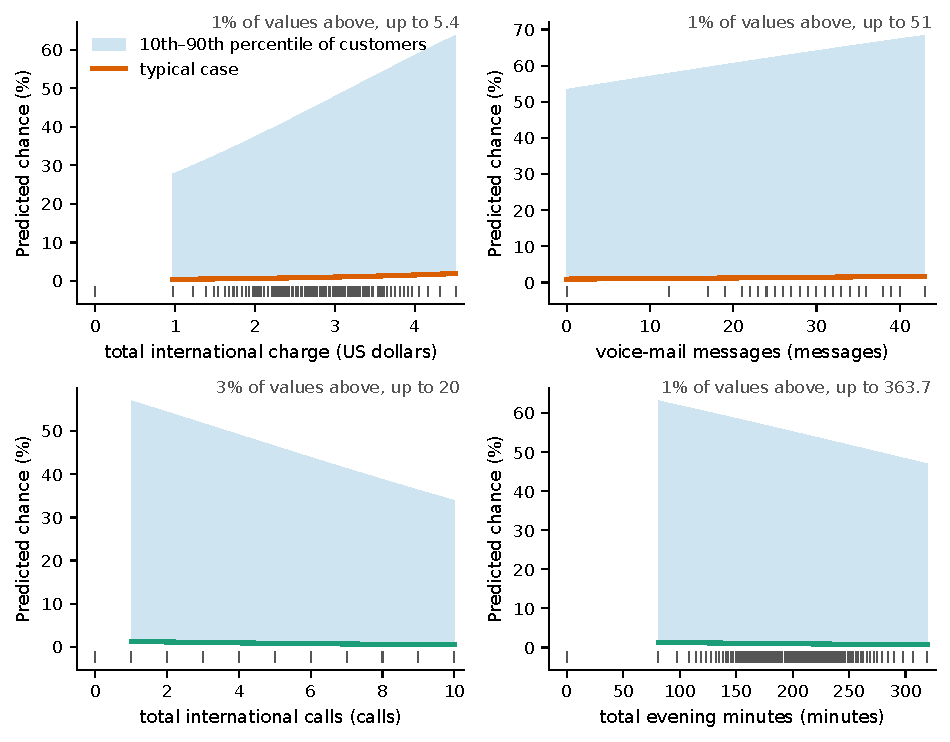
\includegraphics[width=\linewidth,height=0.88\textheight,keepaspectratio]{figures/churn100-s7-c1/ann_78-response.pdf}
\caption{Fixed-weight inputs: Response curves through this part: the typical case (bold), the 10th to 90th percentile of individual customers (band), the fold or step point (dashed) with its spread across them (grey), and the observed values (ticks).}
\label{fig:churn100s7c1:plot-ann78-0}
\end{figure}
\begin{figure}[H]\centering
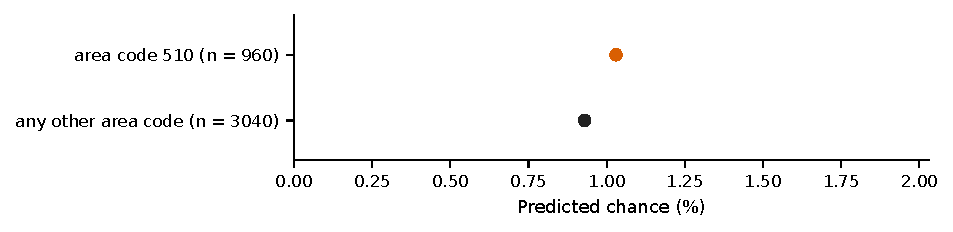
\includegraphics[width=\linewidth,height=0.88\textheight,keepaspectratio]{figures/churn100-s7-c1/ann_78-categories-small.pdf}
\caption{Fixed-weight inputs: The predicted value for the typical case at each level, through this part (n = training customers; grey: fewer than 20).}
\label{fig:churn100s7c1:plot-ann78-1}
\end{figure}
\begin{figure}[H]\centering
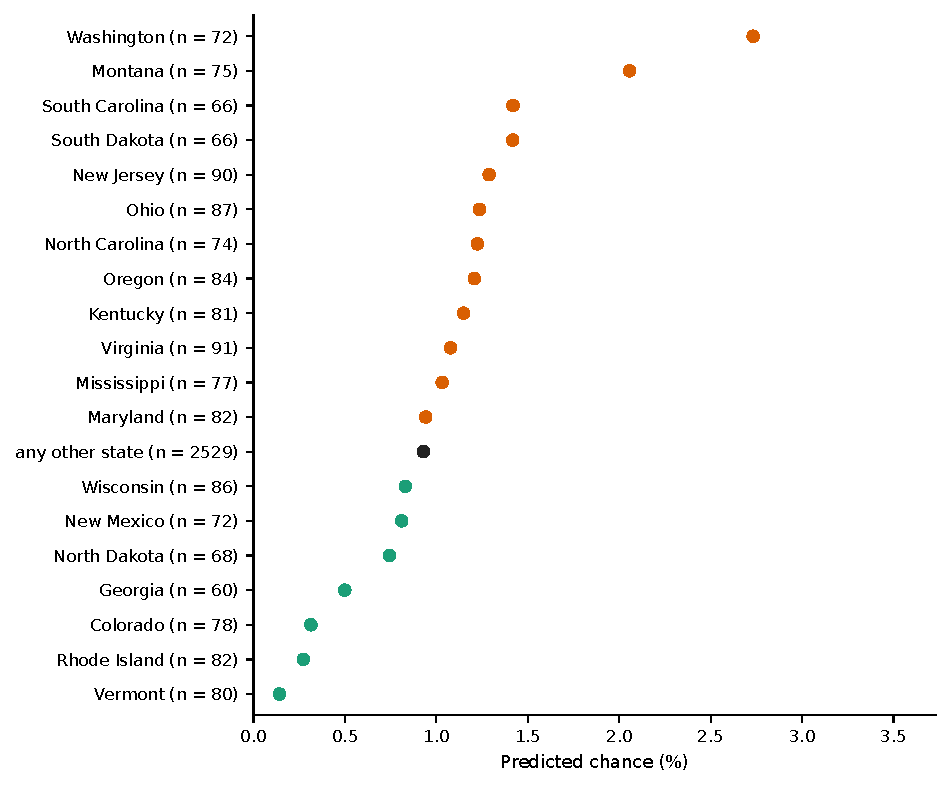
\includegraphics[width=\linewidth,height=0.88\textheight,keepaspectratio]{figures/churn100-s7-c1/ann_78-categories-C080.pdf}
\caption{Fixed-weight inputs: The predicted value for the typical case at each level, through this part (n = training customers; grey: fewer than 20).}
\label{fig:churn100s7c1:plot-ann78-2}
\end{figure}
\begin{figure}[H]\centering
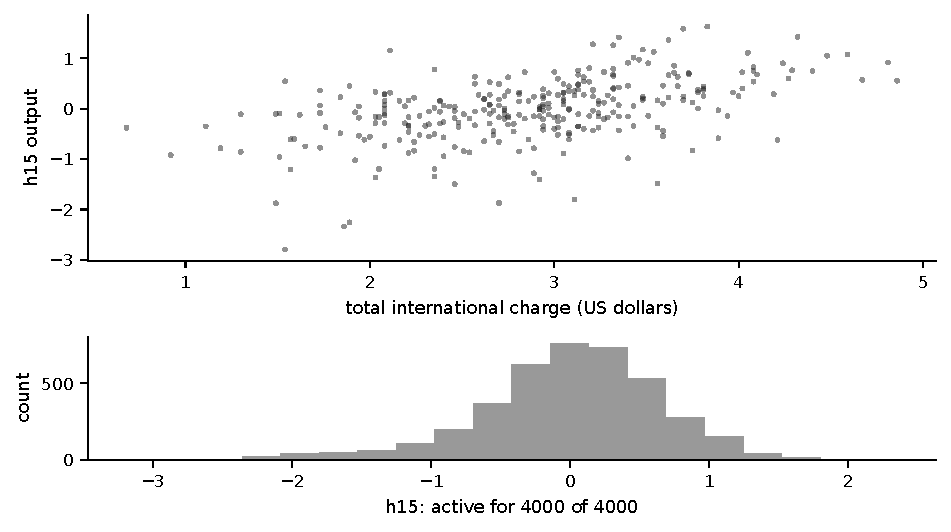
\includegraphics[width=\linewidth,height=0.88\textheight,keepaspectratio]{figures/churn100-s7-c1/ann_78-units.pdf}
\caption{Fixed-weight inputs: This part's hidden units: each unit's output against its main numeric input (top) and how often it is active (bottom).}
\label{fig:churn100s7c1:plot-ann78-3}
\end{figure}
\par\smallskip\noindent{\small Technical detail: \ref{tech:ann78}.\par}
\subsubsection{Voice mail and South Dakota}\label{rd:ann80}
\noindent{\footnotesize Part of: The whole model (\ref{rd:ann84}).\par}
\noindent{\small Figure~\ref{fig:churn100s7c1:parts-ann80} shows what feeds this part; Figure~\ref{fig:churn100s7c1:units-ann80} its units and every connection into them (dashed boxes: connections from or to other parts, drawn in their own sections).\par}
\begin{figure}[H]\centering
\resizebox{!}{\ifdim\height>0.5\textheight 0.5\textheight\else\height\fi}{%
\resizebox{\ifdim\width>\linewidth\linewidth\else\width\fi}{!}{%
\begin{tikzpicture}[
  font=\sffamily\scriptsize, >={Stealth[length=1.6mm]},
  inp/.style={draw, rounded corners=1pt, fill=white, inner sep=1.5pt, minimum height=3.2mm, anchor=east},
  abox/.style={draw, thick, rounded corners=2pt, align=center, inner sep=3pt, minimum height=6mm, text width=42mm},
  outp/.style={draw, double, rounded corners=2pt, fill=white, align=center, inner sep=3pt, text width=24mm},
  agg/.style={draw=black!55},
]
\node[inp] (i0) at (0,0.375) {state};
\node[inp] (i1) at (0,-0.375) {voice-mail plan};
\node[outp] (out) at (9.36,0) {Voice mail and South Dakota};
\begin{scope}[on background layer]
\draw[->, agg, thin, dashed] (i0.east) -- (out.west);
\draw[->, agg, thin, dashed] (i1.east) -- (out.west);
\end{scope}
\end{tikzpicture}}}%
\caption{Voice mail and South Dakota: what feeds it, one level down.}
\label{fig:churn100s7c1:parts-ann80}
\end{figure}
\begin{figure}[H]\centering
\resizebox{\ifdim\width>\linewidth\linewidth\else\width\fi}{!}{%
\definecolor{netup}{HTML}{D95F02}\definecolor{netdown}{HTML}{1B9E77}\definecolor{netmixed}{HTML}{7F7F7F}%
\begin{tikzpicture}[
  font=\sffamily\scriptsize, >={Stealth[length=1.4mm]},
  inp/.style={draw, circle, fill=white, minimum size=3.2mm, inner sep=0pt},
  hid/.style={draw, circle, fill=white, minimum size=5.2mm, inner sep=0.5pt, font=\sffamily\tiny},
  exitbox/.style={draw, thick, rectangle, fill=white, align=center, text width=17mm, minimum height=5mm, inner sep=1.5pt, font=\sffamily\tiny},
  sumbox/.style={draw, thick, dashed, rectangle, fill=white, align=center, text width=17mm, minimum height=5mm, inner sep=1.5pt, font=\sffamily\tiny},
  outp/.style={draw, thick, regular polygon, regular polygon sides=6, fill=white, minimum size=10mm, inner sep=0pt, font=\sffamily\tiny, align=center},
  stub/.style={draw, dashed, rounded corners=2pt, fill=white, align=center, inner sep=2pt, font=\sffamily\tiny, text width=15mm},
  inlab/.style={font=\sffamily\tiny, align=center, text width=15mm, inner sep=1pt, fill=white, fill opacity=0.8, text opacity=1},
  wpos/.style={draw=NavyBlue}, wneg/.style={draw=BrickRed}, wagg/.style={draw=black!45, line width=1.2pt},
  wmix/.style={draw=Plum},
]
\node[exitbox] (n582) at (2.7,1.9) {Voice mail and South Dakota $\downarrow$};
\node[inp, draw=netmixed, very thick] (ngrpxxstate) at (3.6,0.0) {};
\path (ngrpxxstate.south) node[inlab, anchor=north] (labngrpxxstate) {state (23 of 51 used) $\updownarrow$};
\node[inp, draw=netdown, very thick] (ninxxvoicexmailxplan) at (1.8,0.0) {};
\path (ninxxvoicexmailxplan.south) node[inlab, anchor=north] (labninxxvoicexmailxplan) {a voice-mail plan $\downarrow$};
\node[stub] (ntoxxthexmodelxoutput) at (2.7,3.45) {to the model output};
\begin{scope}[on background layer]
\node[fit=(n582) , inner sep=8pt, rounded corners=5pt, fill=Goldenrod!10, draw=Goldenrod!45] (clu0) {};
\draw[->, wpos, line width=0.31pt] (ninxxvoicexmailxplan) -- (n582);
\draw[->, wneg, line width=0.74pt] (n582) -- (ntoxxthexmodelxoutput);
\draw[->, wpos, line width=0.28pt] (ngrpxxstate) -- node[pos=0.8, sloped, above, font=\sffamily\tiny, inner sep=1pt, fill=white, fill opacity=0.8, text opacity=1] {+0.09} (n582);
\end{scope}
\node[font=\sffamily\scriptsize\bfseries, text=Goldenrod!55!black, anchor=south west, inner sep=1pt, fill=white, fill opacity=0.85, text opacity=1] at (clu0.north west) {Voice mail and South Dakota};
\end{tikzpicture}}%
\caption{Voice mail and South Dakota: its units and every connection into them. Blue: positive weight (raises the score); red: negative weight (lowers it); thicker: larger weight. Orange outline and up arrow: raises the final prediction; teal and down arrow: lowers it; grey and double arrow: depends.}
\label{fig:churn100s7c1:units-ann80}
\end{figure}
\paragraph{Hypothesis.} This part lowers the chance of leaving for customers in South Dakota and for customers with a voice-mail plan.\,{\scriptsize\textcolor{NavyBlue}{[C108, C109]}}
\paragraph{Evidence.} Through it, a customer in South Dakota has under 1\% instead of about 1\%, and a voice-mail plan also takes a typical customer to under 1\%.\,{\scriptsize\textcolor{NavyBlue}{[C108, C109]}} Its formula reproduces the part exactly on all 4000 training customers.\,{\scriptsize\textcolor{NavyBlue}{[C110]}}
\par\noindent{\small Evidence plots: Figure~\ref{fig:churn100s7c1:plot-ann80-0}, Figure~\ref{fig:churn100s7c1:plot-ann80-1}.\par}
\begin{figure}[H]\centering
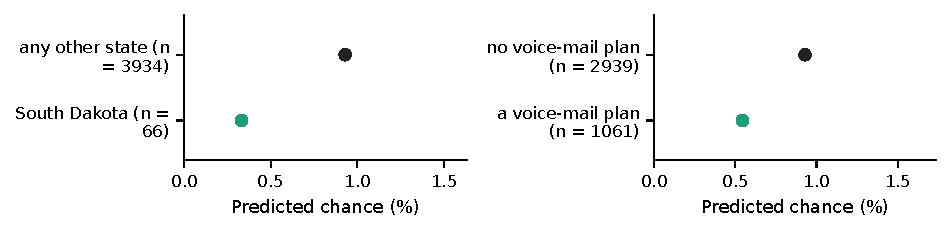
\includegraphics[width=\linewidth,height=0.88\textheight,keepaspectratio]{figures/churn100-s7-c1/ann_80-categories-small.pdf}
\caption{Voice mail and South Dakota: The predicted value for the typical case at each level, through this part (n = training customers; grey: fewer than 20).}
\label{fig:churn100s7c1:plot-ann80-0}
\end{figure}
\begin{figure}[H]\centering
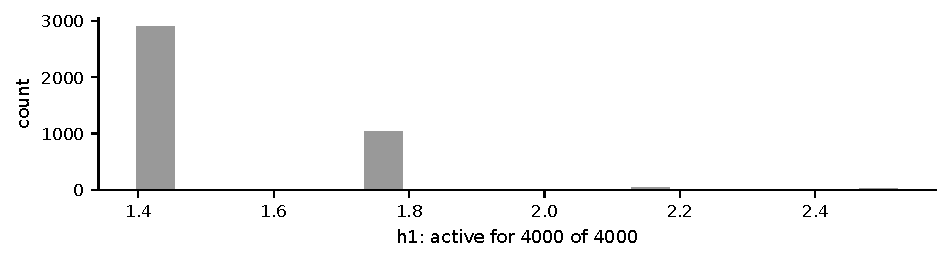
\includegraphics[width=\linewidth,height=0.88\textheight,keepaspectratio]{figures/churn100-s7-c1/ann_80-units.pdf}
\caption{Voice mail and South Dakota: This part's hidden units: each unit's output against its main numeric input (top) and how often it is active (bottom).}
\label{fig:churn100s7c1:plot-ann80-1}
\end{figure}
\par\smallskip\noindent{\small Technical detail: \ref{tech:ann80}.\par}
\subsubsection{State adjustments}\label{rd:ann82}
\noindent{\footnotesize Part of: The whole model (\ref{rd:ann84}).\par}
\noindent{\small Figure~\ref{fig:churn100s7c1:parts-ann82} shows what feeds this part; Figure~\ref{fig:churn100s7c1:units-ann82} its units and every connection into them (dashed boxes: connections from or to other parts, drawn in their own sections).\par}
\begin{figure}[H]\centering
\resizebox{!}{\ifdim\height>0.5\textheight 0.5\textheight\else\height\fi}{%
\resizebox{\ifdim\width>\linewidth\linewidth\else\width\fi}{!}{%
\begin{tikzpicture}[
  font=\sffamily\scriptsize, >={Stealth[length=1.6mm]},
  inp/.style={draw, rounded corners=1pt, fill=white, inner sep=1.5pt, minimum height=3.2mm, anchor=east},
  abox/.style={draw, thick, rounded corners=2pt, align=center, inner sep=3pt, minimum height=6mm, text width=42mm},
  outp/.style={draw, double, rounded corners=2pt, fill=white, align=center, inner sep=3pt, text width=24mm},
  agg/.style={draw=black!55},
]
\node[inp] (i0) at (0,-0.0) {state};
\node[outp] (out) at (9.36,0) {State adjustments};
\begin{scope}[on background layer]
\draw[->, agg, thin, dashed] (i0.east) -- (out.west);
\end{scope}
\end{tikzpicture}}}%
\caption{State adjustments: what feeds it, one level down.}
\label{fig:churn100s7c1:parts-ann82}
\end{figure}
\begin{figure}[H]\centering
\resizebox{\ifdim\width>\linewidth\linewidth\else\width\fi}{!}{%
\definecolor{netup}{HTML}{D95F02}\definecolor{netdown}{HTML}{1B9E77}\definecolor{netmixed}{HTML}{7F7F7F}%
\begin{tikzpicture}[
  font=\sffamily\scriptsize, >={Stealth[length=1.4mm]},
  inp/.style={draw, circle, fill=white, minimum size=3.2mm, inner sep=0pt},
  hid/.style={draw, circle, fill=white, minimum size=5.2mm, inner sep=0.5pt, font=\sffamily\tiny},
  exitbox/.style={draw, thick, rectangle, fill=white, align=center, text width=17mm, minimum height=5mm, inner sep=1.5pt, font=\sffamily\tiny},
  sumbox/.style={draw, thick, dashed, rectangle, fill=white, align=center, text width=17mm, minimum height=5mm, inner sep=1.5pt, font=\sffamily\tiny},
  outp/.style={draw, thick, regular polygon, regular polygon sides=6, fill=white, minimum size=10mm, inner sep=0pt, font=\sffamily\tiny, align=center},
  stub/.style={draw, dashed, rounded corners=2pt, fill=white, align=center, inner sep=2pt, font=\sffamily\tiny, text width=15mm},
  inlab/.style={font=\sffamily\tiny, align=center, text width=15mm, inner sep=1pt, fill=white, fill opacity=0.8, text opacity=1},
  wpos/.style={draw=NavyBlue}, wneg/.style={draw=BrickRed}, wagg/.style={draw=black!45, line width=1.2pt},
  wmix/.style={draw=Plum},
]
\node[hid] (n5667) at (6.35,1.9) {h6};
\node[hid] (n2067) at (4.85,1.9) {h4};
\node[hid] (n5821) at (7.85,1.9) {h7};
\node[hid] (n13164) at (1.85,1.9) {h12};
\node[hid] (n13420) at (3.35,1.9) {h13};
\node[hid] (n12726) at (0.35,1.9) {h11};
\node[inp, draw=netmixed, very thick] (ngrpxxstate) at (4.1,0.0) {};
\path (ngrpxxstate.south) node[inlab, anchor=north] (labngrpxxstate) {state (23 of 51 used) $\updownarrow$};
\node[stub] (ntoxxthexmodelxoutput) at (4.1,3.45) {to the model output};
\begin{scope}[on background layer]
\node[fit=(n5667) (n2067) (n5821) (n13164) (n13420) (n12726) , inner sep=8pt, rounded corners=5pt, fill=Cerulean!10, draw=Cerulean!45] (clu0) {};
\draw[->, wneg, line width=0.34pt] (n2067) -- (ntoxxthexmodelxoutput);
\draw[->, wpos, line width=0.26pt] (n5667) -- (ntoxxthexmodelxoutput);
\draw[->, wneg, line width=0.28pt] (n5821) -- (ntoxxthexmodelxoutput);
\draw[->, wpos, line width=0.26pt] (n12726) -- (ntoxxthexmodelxoutput);
\draw[->, wpos, line width=0.30pt] (n13164) -- (ntoxxthexmodelxoutput);
\draw[->, wneg, line width=0.29pt] (n13420) -- (ntoxxthexmodelxoutput);
\draw[->, wpos, line width=0.61pt] (ngrpxxstate) -- node[pos=0.8, sloped, above, font=\sffamily\tiny, inner sep=1pt, fill=white, fill opacity=0.8, text opacity=1] {+1.02} (n5821);
\draw[->, wneg, line width=0.26pt] (ngrpxxstate) -- node[pos=0.8, sloped, above, font=\sffamily\tiny, inner sep=1pt, fill=white, fill opacity=0.8, text opacity=1] {-0.03} (n5667);
\draw[->, wpos, line width=0.56pt] (ngrpxxstate) -- node[pos=0.8, sloped, above, font=\sffamily\tiny, inner sep=1pt, fill=white, fill opacity=0.8, text opacity=1] {+0.88} (n12726);
\draw[->, wpos, line width=0.60pt] (ngrpxxstate) -- node[pos=0.8, sloped, above, font=\sffamily\tiny, inner sep=1pt, fill=white, fill opacity=0.8, text opacity=1] {+1.01} (n13420);
\draw[->, wpos, line width=0.61pt] (ngrpxxstate) -- node[pos=0.8, sloped, above, font=\sffamily\tiny, inner sep=1pt, fill=white, fill opacity=0.8, text opacity=1] {+1.02} (n13164);
\draw[->, wpos, line width=0.52pt] (ngrpxxstate) -- node[pos=0.8, sloped, above, font=\sffamily\tiny, inner sep=1pt, fill=white, fill opacity=0.8, text opacity=1] {+0.76} (n2067);
\end{scope}
\node[font=\sffamily\scriptsize\bfseries, text=Cerulean!55!black, anchor=south west, inner sep=1pt, fill=white, fill opacity=0.85, text opacity=1] at (clu0.north west) {State adjustments};
\end{tikzpicture}}%
\caption{State adjustments: its units and every connection into them. Blue: positive weight (raises the score); red: negative weight (lowers it); thicker: larger weight. Orange outline and up arrow: raises the final prediction; teal and down arrow: lowers it; grey and double arrow: depends.}
\label{fig:churn100s7c1:units-ann82}
\end{figure}
\paragraph{Hypothesis.} This part shifts the chance of leaving by state: it is lowest in West Virginia and Virginia and highest in South Dakota.\,{\scriptsize\textcolor{NavyBlue}{[C111, C114, C115]}}
\paragraph{Evidence.} Through it, a typical customer's chance is about 5\% in South Dakota and about 2\% in Indiana and in most other states, against about 1\% in West Virginia and under 1\% in Virginia.\,{\scriptsize\textcolor{NavyBlue}{[C111, C112, C114, C115]}} Its formula reproduces the part exactly on all 4000 training customers.\,{\scriptsize\textcolor{NavyBlue}{[C117]}}
\par\noindent{\small Evidence plots: Figure~\ref{fig:churn100s7c1:plot-ann82-0}, Figure~\ref{fig:churn100s7c1:plot-ann82-1}.\par}
\begin{figure}[H]\centering
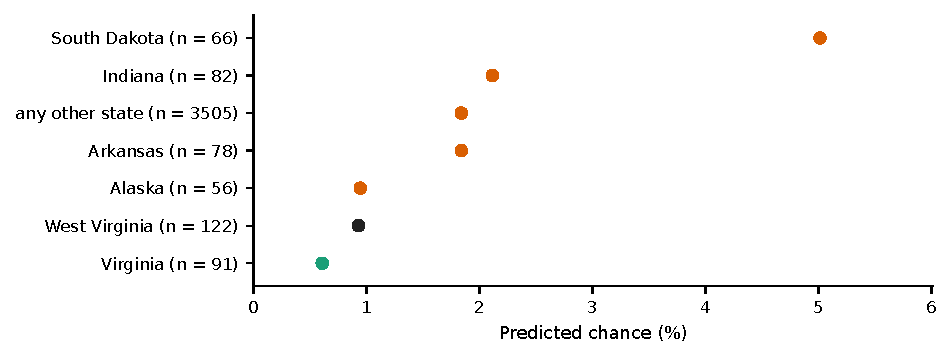
\includegraphics[width=\linewidth,height=0.88\textheight,keepaspectratio]{figures/churn100-s7-c1/ann_82-categories-C111.pdf}
\caption{State adjustments: The predicted value for the typical case at each level, through this part (n = training customers; grey: fewer than 20).}
\label{fig:churn100s7c1:plot-ann82-0}
\end{figure}
\begin{figure}[H]\centering
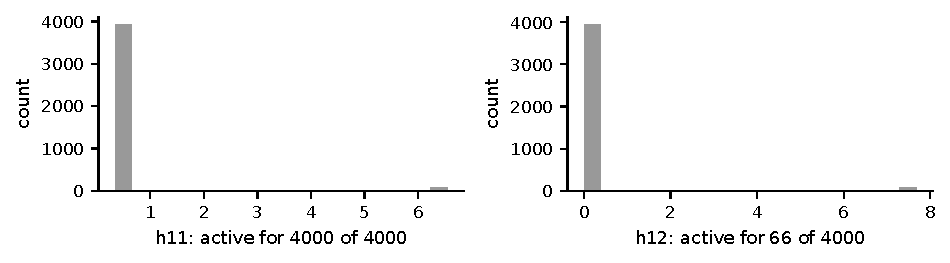
\includegraphics[width=\linewidth,height=0.88\textheight,keepaspectratio]{figures/churn100-s7-c1/ann_82-units.pdf}
\caption{State adjustments: This part's hidden units: each unit's output against its main numeric input (top) and how often it is active (bottom).}
\label{fig:churn100s7c1:plot-ann82-1}
\end{figure}
\par\smallskip\noindent{\small Technical detail: \ref{tech:ann82}.\par}
\subsection{Not supported by the model}
\begin{itemize}\setlength\itemsep{0pt}\small
\item C016: direction claim about total evening minutes in the whole model: not supported by the model (58\% of patients have the opposite sign (allowed: 10\%)).
\item C032: direction claim about total night-time minutes in the whole model: not supported by the model (63\% of patients have the opposite sign (allowed: 10\%)).
\item C058: threshold claim about total night-time minutes in part ann\_\allowbreak{}83: not supported by the model (the folds are spread over 39\% of the observed range (allowed 20\%), also within each category group: no single threshold; the effect past the fold is too small or not consistent across patients).
\item C059: threshold claim about total evening minutes in part ann\_\allowbreak{}83: not supported by the model (the effect past the fold is too small or not consistent across patients; no training patient is past the fold).
\item C069: interaction claim about total daytime minutes and voice-mail plan in part ann\_\allowbreak{}79: not supported by the model (the part's counterfactual difference has the same sign for only 89\% of affected patients).
\item C070: interaction claim about total evening minutes and voice-mail plan in part ann\_\allowbreak{}79: not supported by the model (the part's counterfactual difference has the same sign for only 89\% of affected patients).
\item C073: threshold claim about total night-time minutes in part ann\_\allowbreak{}79: not supported by the model (the folds are spread over 39\% of the observed range (allowed 20\%), also within each category group: no single threshold; the effect past the fold is too small or not consistent across patients).
\item C074: threshold claim about total evening minutes in part ann\_\allowbreak{}79: not supported by the model (the effect past the fold is too small or not consistent across patients; no training patient is past the fold).
\item C075: subgroup claim about state and voice-mail plan in part ann\_\allowbreak{}79: not supported by the model (its effect goes both ways across the patients it acts on).
\item C118: boundary claim about number of calls to customer service and total daytime minutes in part ann\_\allowbreak{}83: not supported by the model (no switch-on line could be traced on the first map to check against the data; no switch-on boundary in the observed range).
\end{itemize}
\clearpage\section*{Technical detail: churn100-s7-c1}
\addcontentsline{toc}{section}{Technical detail: churn100-s7-c1}
\noindent{\small The record behind each part: the original hypothesis, the closed form, and every claim with its estimate (log-odds and odds ratio), range across patients, n and test check.\par}
\renewcommand{\thesubsection}{T.\arabic{subsection}}\setcounter{subsection}{0}
\subsection{The whole model}\label{tech:ann84}
\noindent{\footnotesize Annotation ann\_\allowbreak{}84 (churn\_\allowbreak{}logit). Reads: state, account length, area code, international calling plan, voice-mail plan, number of voice-mail messages, total daytime minutes, total daytime calls, total daytime charge, total evening minutes, total evening calls, total evening charge, total night-time minutes, total night-time calls, total night-time charge, total international minutes, total international calls, total international charge, number of calls to customer service.\par}
\paragraph{Original hypothesis (unchanged).} Root: logit P(churn) = -1.96 + linear\_\allowbreak{}backbone (identity\_\allowbreak{}lin) + usage\_\allowbreak{}response (identity\_\allowbreak{}usage) + 1.68*6711 (intl\_\allowbreak{}plan\_\allowbreak{}switch) - 1.40*582 (vmail\_\allowbreak{}state41\_\allowbreak{}unit) + state\_\allowbreak{}offsets (-0.26*2067 - 0.10*5821 + 0.02*12726 + 0.13*13164 - 0.12*13420 + 0.03*5667), purely additive in the logit; the sigmoid is the only coupling. 35 inputs are unconnected (international minutes, night charge, evening charge and calls, day calls, area codes 408/415 and 29 state indicators) and have zero effect. Train AUC 0.9189, accuracy 0.921. Performance sources (train): all units replaced by least-squares linear fits gives AUC 0.8336 (an L2 logistic regression refit on all 71 inputs gets 0.8433); restoring usage\_\allowbreak{}response alone gives 0.9189 (all the gain); its parts alone: usage hinge 0.8803, heavy-use hinge 0.8870, service-calls gate 0.8731. The international-plan, voicemail and state units are exact switches/offsets and restore nothing. Rare-category switches: state:46 -1.89 logit (80 rows, empirical log-odds offset -0.91); state:39 -1.23 (82, -0.93); state:47 +1.10 (72, +0.92); state:5 -1.09 (78, -0.51); state:45 -0.97 (91, -0.85); state:26 +0.81 (75, +0.50); state:49 -0.69 (122, -0.32); state:0 -0.68 (56, -0.76); state:10 -0.63 (60, -0.22); state:41 +0.25 mean, range -3.85..+0.43 (66, -0.04: it switches off the 1406 day-charge hinge, so heavy users lose up to 3.85).
\paragraph{Closed form.} Read through its parts (their formulas are in their own sections).
\paragraph{Split inputs.} To annotate the parts, the explanation split these inputs into copies (a refactoring step that does not change what the model computes); the diagrams draw each input once: total evening minutes (2 copies); total night-time minutes (2 copies); a voice-mail plan (2 copies).
\paragraph{State: every level the model reads.} Whole-model change in the predicted chance for a typical customer when only the state changes from the reference; n = training customers in that level.\par\smallskip
{\scriptsize\rowcolors{2}{black!6}{white}
\begin{longtable}{@{}lllrlc@{}}
\toprule\rowcolor{white}
Claim & From & To & n & Chance & OK \\
\midrule\endhead
\bottomrule\endfoot
C002 & West Virginia & Washington & 72 & 1\% to 5\% & \textcolor{OliveGreen}{yes} \\
C003 & West Virginia & Montana & 75 & 1\% to 4\% & \textcolor{OliveGreen}{yes} \\
C006 & West Virginia & South Carolina & 66 & 1\% to 3\% & \textcolor{OliveGreen}{yes} \\
C007 & West Virginia & South Dakota & 66 & 1\% to 3\% & \textcolor{OliveGreen}{yes} \\
C008 & West Virginia & New Jersey & 90 & 1\% to 3\% & \textcolor{OliveGreen}{yes} \\
C009 & West Virginia & Ohio & 87 & 1\% to 2\% & \textcolor{OliveGreen}{yes} \\
C010 & West Virginia & North Carolina & 74 & 1\% to 2\% & \textcolor{OliveGreen}{yes} \\
C011 & West Virginia & Oregon & 84 & 1\% to 2\% & \textcolor{OliveGreen}{yes} \\
C012 & West Virginia & Kentucky & 81 & 1\% to 2\% & \textcolor{OliveGreen}{yes} \\
C013 & West Virginia & Indiana & 82 & 1\% to 2\% & \textcolor{OliveGreen}{yes} \\
C014 & West Virginia & Mississippi & 77 & 1\% to 2\% & \textcolor{OliveGreen}{yes} \\
C015 & West Virginia & Maryland & 82 & 1\% to 2\% & \textcolor{OliveGreen}{yes} \\
C017 & West Virginia & Arkansas & 78 & 1\% to 2\% & \textcolor{OliveGreen}{yes} \\
C018 & West Virginia & state other than Alaska, Georgia, Indiana, Kentucky, Arka... & 2191 & 1\% to 2\% & \textcolor{OliveGreen}{yes} \\
C020 & West Virginia & Wisconsin & 86 & 1\% to 2\% & \textcolor{OliveGreen}{yes} \\
C021 & West Virginia & New Mexico & 72 & 1\% to 2\% & \textcolor{OliveGreen}{yes} \\
C024 & West Virginia & North Dakota & 68 & 1\% to 1\% & \textcolor{OliveGreen}{yes} \\
C034 & West Virginia & Georgia & 60 & 1\% to 1\% & \textcolor{OliveGreen}{yes} \\
C036 & West Virginia & Alaska & 56 & 1\% to 1\% & \textcolor{OliveGreen}{yes} \\
C030 & West Virginia & Virginia & 91 & 1\% to 1\% & \textcolor{OliveGreen}{yes} \\
C028 & West Virginia & Colorado & 78 & 1\% to 1\% & \textcolor{OliveGreen}{yes} \\
C026 & West Virginia & Rhode Island & 82 & 1\% to 1\% & \textcolor{OliveGreen}{yes} \\
C022 & West Virginia & Vermont & 80 & 1\% to $<$1\% & \textcolor{OliveGreen}{yes} \\
\end{longtable}}
\paragraph{Evidence table} (next page, landscape).
\begin{landscape}
{\scriptsize\setlength{\tabcolsep}{3pt}\renewcommand{\arraystretch}{1.15}
\rowcolors{2}{black!6}{white}
\begin{longtable}{@{}l>{\raggedright\arraybackslash}p{0.36\linewidth}>{\raggedright\arraybackslash}p{0.14\linewidth}rrr>{\raggedright\arraybackslash}p{0.06\linewidth}>{\raggedright\arraybackslash}p{0.17\linewidth}c@{}}
\toprule\rowcolor{white}
ID & What is checked & Risk, typical patient & Log-odds & OR & Range (p10--p90) & n & Test check & OK \\
\midrule\endfirsthead
\toprule\rowcolor{white}
ID & What is checked & Risk, typical patient & Log-odds & OR & Range (p10--p90) & n & Test check & OK \\
\midrule\endhead
\bottomrule\endfoot
C001 & direction: international calling plan: no international plan to an international plan (whole model) \newline{\itshape shape: categorical; highest to lowest: an international plan, no international plan} & 1\% to 15\% & 2.91 & 18.3 & 2.91 to 2.91 & 3620, 380 & agrees; AUC gain 0.060 [0.033, 0.090] & \textcolor{OliveGreen}{yes} \\
C002 & direction: state: West Virginia to Washington (whole model) \newline{\itshape shape: categorical; highest to lowest: Washington, Montana, South Carolina, South Dakota, New Jersey, Ohio ...} & 1\% to 5\% & 1.79 & 5.98 & 1.79 to 1.79 & 122, 72 & disagrees; AUC gain -0.004 [-0.017, 0.006] & \textcolor{OliveGreen}{yes} \\
C003 & direction: state: West Virginia to Montana (whole model) \newline{\itshape shape: categorical; highest to lowest: Washington, Montana, South Carolina, South Dakota, New Jersey, Ohio ...} & 1\% to 4\% & 1.50 & 4.47 & 1.50 to 1.50 & 122, 75 & disagrees; AUC gain -0.004 [-0.017, 0.006] & \textcolor{OliveGreen}{yes} \\
C004 & direction: total daytime minutes: 112 minutes to 249 minutes (whole model) \newline{\itshape shape: accelerating; 67\% of patients same; fallback; risk saturates near 0\%} & 1\% to 4\% & 1.37 & 3.93 & 0.00 to 4.32 & 4000 & agrees; AUC gain 0.035 [0.016, 0.052] & \textcolor{OliveGreen}{yes} \\
C005 & direction: customer-service calls: 0 calls to 3 calls (whole model) \newline{\itshape shape: accelerating; 89\% of patients same; mixed (but hinge for customers without a voice-mail plan); risk saturates near 0\%} & 1\% to 3\% & 0.86 & 2.37 & 0.00 to 1.25 & 4000 & agrees; AUC gain 0.097 [0.061, 0.136] & \textcolor{OliveGreen}{yes} \\
C006 & direction: state: West Virginia to South Carolina (whole model) \newline{\itshape shape: categorical; highest to lowest: Washington, Montana, South Carolina, South Dakota, New Jersey, Ohio ...} & 1\% to 3\% & 1.12 & 3.06 & 1.12 to 1.12 & 122, 66 & disagrees; AUC gain -0.004 [-0.017, 0.006] & \textcolor{OliveGreen}{yes} \\
C007 & direction: state: West Virginia to South Dakota (whole model) \newline{\itshape shape: categorical; highest to lowest: Washington, Montana, South Carolina, South Dakota, New Jersey, Ohio ...} & 1\% to 3\% & 0.94 & 2.55 & 0.79 to 1.12 & 122, 66 & disagrees; AUC gain -0.004 [-0.017, 0.006] & \textcolor{OliveGreen}{yes} \\
C008 & direction: state: West Virginia to New Jersey (whole model) \newline{\itshape shape: categorical; highest to lowest: Washington, Montana, South Carolina, South Dakota, New Jersey, Ohio ...} & 1\% to 3\% & 1.02 & 2.78 & 1.02 to 1.02 & 122, 90 & disagrees; AUC gain -0.004 [-0.017, 0.006] & \textcolor{OliveGreen}{yes} \\
C009 & direction: state: West Virginia to Ohio (whole model) \newline{\itshape shape: categorical; highest to lowest: Washington, Montana, South Carolina, South Dakota, New Jersey, Ohio ...} & 1\% to 2\% & 0.98 & 2.66 & 0.98 to 0.98 & 122, 87 & disagrees; AUC gain -0.004 [-0.017, 0.006] & \textcolor{OliveGreen}{yes} \\
C010 & direction: state: West Virginia to North Carolina (whole model) \newline{\itshape shape: categorical; highest to lowest: Washington, Montana, South Carolina, South Dakota, New Jersey, Ohio ...} & 1\% to 2\% & 0.97 & 2.64 & 0.97 to 0.97 & 122, 74 & disagrees; AUC gain -0.004 [-0.017, 0.006] & \textcolor{OliveGreen}{yes} \\
C011 & direction: state: West Virginia to Oregon (whole model) \newline{\itshape shape: categorical; highest to lowest: Washington, Montana, South Carolina, South Dakota, New Jersey, Ohio ...} & 1\% to 2\% & 0.96 & 2.60 & 0.96 to 0.96 & 122, 84 & disagrees; AUC gain -0.004 [-0.017, 0.006] & \textcolor{OliveGreen}{yes} \\
C012 & direction: state: West Virginia to Kentucky (whole model) \newline{\itshape shape: categorical; highest to lowest: Washington, Montana, South Carolina, South Dakota, New Jersey, Ohio ...} & 1\% to 2\% & 0.91 & 2.47 & 0.91 to 0.91 & 122, 81 & disagrees; AUC gain -0.004 [-0.017, 0.006] & \textcolor{OliveGreen}{yes} \\
C013 & direction: state: West Virginia to Indiana (whole model) \newline{\itshape shape: categorical; highest to lowest: Washington, Montana, South Carolina, South Dakota, New Jersey, Ohio ...} & 1\% to 2\% & 0.83 & 2.30 & 0.83 to 0.83 & 122, 82 & disagrees; AUC gain -0.004 [-0.017, 0.006] & \textcolor{OliveGreen}{yes} \\
C014 & direction: state: West Virginia to Mississippi (whole model) \newline{\itshape shape: categorical; highest to lowest: Washington, Montana, South Carolina, South Dakota, New Jersey, Ohio ...} & 1\% to 2\% & 0.80 & 2.22 & 0.80 to 0.80 & 122, 77 & disagrees; AUC gain -0.004 [-0.017, 0.006] & \textcolor{OliveGreen}{yes} \\
C015 & direction: state: West Virginia to Maryland (whole model) \newline{\itshape shape: categorical; highest to lowest: Washington, Montana, South Carolina, South Dakota, New Jersey, Ohio ...} & 1\% to 2\% & 0.70 & 2.02 & 0.70 to 0.70 & 122, 82 & disagrees; AUC gain -0.004 [-0.017, 0.006] & \textcolor{OliveGreen}{yes} \\
C016 & direction: total evening minutes: 138 minutes to 266 minutes (whole model) \newline{\itshape shape: dip at 212 minutes; 36\% of patients same; fallback; risk saturates near 0\%} & 1\% to 2\% & 0.67 & 1.96 & -0.35 to 3.65 & 4000 & agrees; AUC gain 0.030 [0.010, 0.050] & \textcolor{BrickRed}{no} \\
C017 & direction: state: West Virginia to Arkansas (whole model) \newline{\itshape shape: categorical; highest to lowest: Washington, Montana, South Carolina, South Dakota, New Jersey, Ohio ...} & 1\% to 2\% & 0.69 & 2.00 & 0.69 to 0.69 & 122, 78 & disagrees; AUC gain -0.004 [-0.017, 0.006] & \textcolor{OliveGreen}{yes} \\
C018 & direction: state: West Virginia to state other than Alaska, Georgia, Indiana, Kentucky, Arkansas, Maryland, Mississippi, Montana, North Carolina, North Dakota, New Jersey, New Mexico, Ohio, Oregon, Rhode Island, South Carolina, South Dakota, Virginia, Vermont, Washington, Wisconsin, West Virginia, Colorado (whole model) \newline{\itshape shape: categorical; highest to lowest: Washington, Montana, South Carolina, South Dakota, New Jersey, Ohio ...} & 1\% to 2\% & 0.69 & 2.00 & 0.69 to 0.69 & 122, 2191 & disagrees; AUC gain -0.004 [-0.017, 0.006] & \textcolor{OliveGreen}{yes} \\
C019 & direction: total international charge: 1.84 US dollars to 3.70 US dollars (whole model) \newline{\itshape shape: steady; 100\% of patients same; verified; risk saturates near 0\%} & 1\% to 1\% & 0.80 & 2.23 & 0.80 to 0.80 & 4000 & unclear; AUC gain 0.003 [-0.005, 0.011] & \textcolor{OliveGreen}{yes} \\
C020 & direction: state: West Virginia to Wisconsin (whole model) \newline{\itshape shape: categorical; highest to lowest: Washington, Montana, South Carolina, South Dakota, New Jersey, Ohio ...} & 1\% to 2\% & 0.58 & 1.78 & 0.58 to 0.58 & 122, 86 & disagrees; AUC gain -0.004 [-0.017, 0.006] & \textcolor{OliveGreen}{yes} \\
C021 & direction: state: West Virginia to New Mexico (whole model) \newline{\itshape shape: categorical; highest to lowest: Washington, Montana, South Carolina, South Dakota, New Jersey, Ohio ...} & 1\% to 2\% & 0.55 & 1.74 & 0.55 to 0.55 & 122, 72 & disagrees; AUC gain -0.004 [-0.017, 0.006] & \textcolor{OliveGreen}{yes} \\
C022 & direction: state: West Virginia to Vermont (whole model) \newline{\itshape shape: categorical; highest to lowest: Washington, Montana, South Carolina, South Dakota, New Jersey, Ohio ...} & 1\% to $<$1\% & -1.20 & 0.30 & -1.20 to -1.20 & 122, 80 & disagrees; AUC gain -0.004 [-0.017, 0.006] & \textcolor{OliveGreen}{yes} \\
C023 & direction: voice-mail messages: 0 messages to 32 messages (whole model) \newline{\itshape shape: steady; 100\% of patients same; verified; risk saturates near 0\%} & 1\% to 1\% & 0.47 & 1.60 & 0.47 to 0.47 & 4000 & unclear; AUC gain 0.0008 [-0.004, 0.006] & \textcolor{OliveGreen}{yes} \\
C024 & direction: state: West Virginia to North Dakota (whole model) \newline{\itshape shape: categorical; highest to lowest: Washington, Montana, South Carolina, South Dakota, New Jersey, Ohio ...} & 1\% to 1\% & 0.47 & 1.60 & 0.47 to 0.47 & 122, 68 & disagrees; AUC gain -0.004 [-0.017, 0.006] & \textcolor{OliveGreen}{yes} \\
C025 & direction: total international calls: 2 calls to 8 calls (whole model) \newline{\itshape shape: steady (equal steps); 100\% of patients same; verified; risk saturates near 0\%} & 1\% to 1\% & -0.63 & 0.53 & -0.63 to -0.63 & 4000 & unclear; AUC gain 0.002 [-0.004, 0.008] & \textcolor{OliveGreen}{yes} \\
C026 & direction: state: West Virginia to Rhode Island (whole model) \newline{\itshape shape: categorical; highest to lowest: Washington, Montana, South Carolina, South Dakota, New Jersey, Ohio ...} & 1\% to 1\% & -0.54 & 0.58 & -0.54 to -0.54 & 122, 82 & disagrees; AUC gain -0.004 [-0.017, 0.006] & \textcolor{OliveGreen}{yes} \\
C027 & direction: voice-mail plan: no voice-mail plan to a voice-mail plan (whole model) \newline{\itshape shape: categorical; highest to lowest: no voice-mail plan, a voice-mail plan} & 1\% to 1\% & -1.37 & 0.25 & -3.46 to -0.54 & 2939, 1061 & agrees; AUC gain 0.019 [0.005, 0.031] & \textcolor{OliveGreen}{yes} \\
C028 & direction: state: West Virginia to Colorado (whole model) \newline{\itshape shape: categorical; highest to lowest: Washington, Montana, South Carolina, South Dakota, New Jersey, Ohio ...} & 1\% to 1\% & -0.40 & 0.67 & -0.40 to -0.40 & 122, 78 & disagrees; AUC gain -0.004 [-0.017, 0.006] & \textcolor{OliveGreen}{yes} \\
C029 & direction: total daytime charge: 19.07 US dollars to 42.40 US dollars (whole model) \newline{\itshape shape: hinge at 40.06 US dollars; 50\% of patients same; fallback; risk saturates near 0\%; matches the fold at 38.81 US dollars} & 1\% to 1\% & 0.24 & 1.27 & 0.00 to 1.11 & 4000 & unclear; AUC gain 0.0003 [-0.007, 0.008] & \textcolor{OliveGreen}{yes} \\
C030 & direction: state: West Virginia to Virginia (whole model) \newline{\itshape shape: categorical; highest to lowest: Washington, Montana, South Carolina, South Dakota, New Jersey, Ohio ...} & 1\% to 1\% & -0.28 & 0.76 & -0.28 to -0.28 & 122, 91 & disagrees; AUC gain -0.004 [-0.017, 0.006] & \textcolor{OliveGreen}{yes} \\
C031 & direction: account length: 48 to 152 (whole model) \newline{\itshape shape: steady; 100\% of patients same; verified; risk saturates near 0\%} & 1\% to 1\% & 0.23 & 1.26 & 0.23 to 0.23 & 4000 & disagrees; AUC gain -0.001 [-0.003, 0.001] & \textcolor{OliveGreen}{yes} \\
C032 & direction: total night-time minutes: 136 minutes to 264 minutes (whole model) \newline{\itshape shape: dip at 218 minutes; 30\% of patients same; fallback; risk saturates near 0\%} & 1\% to 1\% & 0.34 & 1.40 & -0.29 to 2.38 & 4000 & agrees; AUC gain 0.007 [0.0006, 0.013] & \textcolor{BrickRed}{no} \\
C033 & direction: area code: area code other than area code 510 to area code 510 (whole model) \newline{\itshape shape: categorical; highest to lowest: area code 510, area code other than area code 510} & 1\% to 1\% & 0.10 & 1.11 & 0.10 to 0.10 & 3040, 960 & unclear; AUC gain 8e-05 [-0.001, 0.002] & \textcolor{OliveGreen}{yes} \\
C034 & direction: state: West Virginia to Georgia (whole model) \newline{\itshape shape: categorical; highest to lowest: Washington, Montana, South Carolina, South Dakota, New Jersey, Ohio ...} & 1\% to 1\% & 0.07 & 1.07 & 0.07 to 0.07 & 122, 60 & disagrees; AUC gain -0.004 [-0.017, 0.006] & \textcolor{OliveGreen}{yes} \\
C035 & direction: total night-time calls: 74 calls to 125 calls (whole model) \newline{\itshape shape: steady; 100\% of patients same; verified; risk saturates near 0\%} & 1\% to 1\% & 0.06 & 1.07 & 0.06 to 0.06 & 4000 & disagrees; AUC gain -9e-05 [-0.0008, 0.0006] & \textcolor{OliveGreen}{yes} \\
C036 & direction: state: West Virginia to Alaska (whole model) \newline{\itshape shape: categorical; highest to lowest: Washington, Montana, South Carolina, South Dakota, New Jersey, Ohio ...} & 1\% to 1\% & 0.02 & 1.02 & 0.02 to 0.02 & 122, 56 & disagrees; AUC gain -0.004 [-0.017, 0.006] & \textcolor{OliveGreen}{yes} \\
C037 & magnitude: international calling plan: no international plan to an international plan, typical patient \newline{\itshape shape: categorical; highest to lowest: an international plan, no international plan} & 1\% to 15\% & 2.91 & 18.3 &  & 3620, 380 & agrees; AUC gain 0.060 [0.033, 0.090] & \textcolor{OliveGreen}{yes} \\
C038 & magnitude: state: West Virginia to Washington, typical patient \newline{\itshape shape: categorical; highest to lowest: Washington, Montana, South Carolina, South Dakota, New Jersey, Ohio ...} & 1\% to 5\% & 1.79 & 5.98 &  & 122, 72 & disagrees; AUC gain -0.004 [-0.017, 0.006] & \textcolor{OliveGreen}{yes} \\
C039 & magnitude: total daytime minutes: 112 minutes to 249 minutes, typical patient \newline{\itshape shape: accelerating; 67\% of patients same; fallback; risk saturates near 0\%} & 1\% to 4\% & 1.47 & 4.37 &  & 4000 & agrees; AUC gain 0.035 [0.016, 0.052] & \textcolor{OliveGreen}{yes} \\
C040 & magnitude: customer-service calls: 0 calls to 3 calls, typical patient \newline{\itshape shape: accelerating; 89\% of patients same; mixed (but hinge for customers without a voice-mail plan); risk saturates near 0\%} & 1\% to 3\% & 1.25 & 3.50 &  & 4000 & agrees; AUC gain 0.097 [0.061, 0.136] & \textcolor{OliveGreen}{yes} \\
C041 & magnitude: total international charge: 1.84 US dollars to 3.70 US dollars, typical patient \newline{\itshape shape: steady; 100\% of patients same; verified; risk saturates near 0\%} & 1\% to 1\% & 0.80 & 2.23 &  & 4000 & unclear; AUC gain 0.003 [-0.005, 0.011] & \textcolor{OliveGreen}{yes} \\
C042 & null: model ignores total daytime calls (exact rule) &  & 0.00 &  &  & 4000 & train only & \textcolor{OliveGreen}{yes} \\
C043 & null: model ignores total evening calls (exact rule) &  & 0.00 &  &  & 4000 & train only & \textcolor{OliveGreen}{yes} \\
C044 & null: model ignores total evening charge (exact rule) &  & 0.00 &  &  & 4000 & train only & \textcolor{OliveGreen}{yes} \\
C045 & null: model ignores total international minutes (exact rule) &  & 0.00 &  &  & 4000 & train only & \textcolor{OliveGreen}{yes} \\
C046 & null: model ignores total night-time charge (exact rule) &  & 0.00 &  &  & 4000 & train only & \textcolor{OliveGreen}{yes} \\
C047 & structure: made of linear\_\allowbreak{}backbone, usage\_\allowbreak{}response, intl\_\allowbreak{}plan\_\allowbreak{}switch, vmail\_\allowbreak{}state41\_\allowbreak{}unit, state\_\allowbreak{}offsets; added &  &  &  &  & 4000 & train only & \textcolor{OliveGreen}{yes} \\
\end{longtable}}
\end{landscape}
\subsection{Usage and service calls}\label{tech:ann83}
\noindent{\footnotesize Annotation ann\_\allowbreak{}83 (usage\_\allowbreak{}response). Reads: state, voice-mail plan, total daytime minutes, total daytime charge, total evening minutes, total night-time minutes, number of calls to customer service.\par}
\paragraph{Original hypothesis (unchanged).} Composition on usage\_\allowbreak{}hinge: identity\_\allowbreak{}usage = 2.57*879 + 3.06*10552 + 2.88*4344 enters the logit with weight 1. 10552 = relu(-0.64 + 1.17*relu(-0.16 + 1.08*879)) is a second, steeper hinge that opens once 879 exceeds 0.65 (about 240 day minutes at median other use; active for 12\% of customers), so the usage effect accelerates. 4344 = relu(-0.38 + 0.75 calls - 3.24*879) is a service-calls gate: shut for 0-2 calls, open from 3 calls, and closed again by usage (at 3 calls once 879 $>$ 0.14, at 5 calls once 879 $>$ 0.49). Hypothesis: usage and service calls interact non-additively: service calls raise churn only for low-usage customers (or voicemail-plan customers, for whom usage is off), heavy users get the usage hinges instead. Evidence (train): usage logit (879+10552) by day minutes 0.14 ($<$200), 0.58 (200-220), 1.08 (220-240), 2.02 (240-260), 3.43 (260-280), 6.37 ($>$=280); churn 0.10/\allowbreak{}0.06/\allowbreak{}0.14/\allowbreak{}0.26/\allowbreak{}0.46/\allowbreak{}0.67 vs model 0.09/\allowbreak{}0.09/\allowbreak{}0.17/\allowbreak{}0.30/\allowbreak{}0.49/\allowbreak{}0.69. Without a voicemail plan churn reaches 0.84 above 280 minutes (model 0.86), with a plan 0.04 (model 0.09). Gate logit at 0-7 calls: 0/\allowbreak{}0/\allowbreak{}0/\allowbreak{}0.80/\allowbreak{}2.11/\allowbreak{}3.59/\allowbreak{}5.30/\allowbreak{}7.08 (1.25/2.90/4.55/6.20 at 3-6 calls when usage is off, 0.10/0.50/1.05/2.01 when it is on). Churn by calls 0.115/\allowbreak{}0.110/\allowbreak{}0.110/\allowbreak{}0.106/\allowbreak{}0.437/\allowbreak{}0.571/\allowbreak{}0.679/\allowbreak{}0.545 vs model 0.116/\allowbreak{}0.111/\allowbreak{}0.109/\allowbreak{}0.150/\allowbreak{}0.319/\allowbreak{}0.598/\allowbreak{}0.849/\allowbreak{}0.940: the gate opens one call too early (3 calls: +0.80 logit, empirical churn unchanged) and is over-confident from 6 calls (39 customers). Mean ablation of all three terms AUC 0.6557 (the largest drop: full 0.9189); gate alone 0.8202, heavy-use hinge alone 0.9093; linear replacement 0.8336 (R2 0.53/0.29/0.53); restoring usage\_\allowbreak{}response alone onto the all-linear model recovers 0.9189 (all-linear 0.8336), i.e. all of the gain.
\paragraph{Closed form.} Read through its parts (their formulas are in their own sections).
\paragraph{Evidence table} (next page, landscape).
\begin{landscape}
{\scriptsize\setlength{\tabcolsep}{3pt}\renewcommand{\arraystretch}{1.15}
\rowcolors{2}{black!6}{white}
\begin{longtable}{@{}l>{\raggedright\arraybackslash}p{0.36\linewidth}>{\raggedright\arraybackslash}p{0.14\linewidth}rrr>{\raggedright\arraybackslash}p{0.06\linewidth}>{\raggedright\arraybackslash}p{0.17\linewidth}c@{}}
\toprule\rowcolor{white}
ID & What is checked & Risk, typical patient & Log-odds & OR & Range (p10--p90) & n & Test check & OK \\
\midrule\endfirsthead
\toprule\rowcolor{white}
ID & What is checked & Risk, typical patient & Log-odds & OR & Range (p10--p90) & n & Test check & OK \\
\midrule\endhead
\bottomrule\endfoot
C048 & direction: total daytime minutes: 112 minutes to 249 minutes (through this part) \newline{\itshape shape: accelerating; 67\% of patients same; fallback; risk saturates near 0\%} & 1\% to 4\% & 1.37 & 3.93 & 0.00 to 4.32 & 4000 & agrees; AUC gain 0.035 [0.016, 0.052] & \textcolor{OliveGreen}{yes} \\
C049 & direction: customer-service calls: 0 calls to 3 calls (through this part) \newline{\itshape shape: accelerating; 89\% of patients same; mixed (but hinge for customers without a voice-mail plan); risk saturates near 0\%} & 1\% to 3\% & 0.86 & 2.37 & 0.00 to 1.25 & 4000 & agrees; AUC gain 0.097 [0.061, 0.136] & \textcolor{OliveGreen}{yes} \\
C050 & direction: total evening minutes: 138 minutes to 266 minutes (through this part) \newline{\itshape shape: accelerating; 40\% of patients same; fallback; risk saturates near 0\%} & 1\% to 2\% & 1.03 & 2.79 & 0.00 to 4.01 & 4000 & agrees; AUC gain 0.034 [0.013, 0.055] & \textcolor{OliveGreen}{yes} \\
C051 & direction: total night-time minutes: 136 minutes to 264 minutes (through this part) \newline{\itshape shape: hinge at 224 minutes; 35\% of patients same; fallback; risk saturates near 0\%} & 1\% to 1\% & 0.63 & 1.87 & 0.00 to 2.67 & 4000 & agrees; AUC gain 0.01 [0.003, 0.016] & \textcolor{OliveGreen}{yes} \\
C052 & direction: total daytime charge: 19.07 US dollars to 42.40 US dollars (through this part) \newline{\itshape shape: hinge at 38.81 US dollars; 50\% of patients same; fallback; risk saturates near 0\%; one point with C057 (median fold 38.81 US dollars, typical patient 40.06 US dollars, 10th-90th percentile 37.22 US dollars to 53.94 US dollars, wide)} & 1\% to 1\% & 0.24 & 1.27 & 0.00 to 1.11 & 4000 & unclear; AUC gain 0.0003 [-0.007, 0.008] & \textcolor{OliveGreen}{yes} \\
C053 & direction: state: state other than South Dakota to South Dakota (through this part) \newline{\itshape shape: categorical; highest to lowest: South Dakota, state other than South Dakota} & 1\% to 1\% & -0.18 & 0.83 & -0.32 to 0.00 & 3934, 66 & unclear; AUC gain 0.0002 [-0.0002, 0.0007] & \textcolor{OliveGreen}{yes} \\
C054 & direction: voice-mail plan: no voice-mail plan to a voice-mail plan (through this part) \newline{\itshape shape: categorical; highest to lowest: a voice-mail plan, no voice-mail plan} & 1\% to 1\% & -0.83 & 0.44 & -2.92 to 0.00 & 2939, 1061 & agrees; AUC gain 0.013 [0.0009, 0.023] & \textcolor{OliveGreen}{yes} \\
C055 & threshold: customer-service calls: fold at about 3 calls (starts) \newline{\itshape shape: accelerating; 86\% of patients same; mixed (but hinge for customers without a voice-mail plan); risk saturates near 0\%} & 1\% to 15\% (typical patient with a fold) & 2.20 & 9.02 & 0.00 to 2.90 & 3833, 614 & agrees; AUC gain 0.097 [0.061, 0.136] & \textcolor{OliveGreen}{yes} \\
C056 & threshold: total daytime minutes: fold at about 187 minutes (starts) for customers without a voice-mail plan \newline{\itshape shape: accelerating; 67\% of patients same; fallback; risk saturates near 0\%} & 1\% to 11\% (typical patient with a fold) & 2.80 & 16.4 & 0.00 to 6.18 & 3014, 1382 & agrees; AUC gain 0.035 [0.016, 0.052] & \textcolor{OliveGreen}{yes} \\
C057 & threshold: total daytime charge: fold at about 38.81 US dollars (starts) for customers without a voice-mail plan \newline{\itshape shape: hinge at 38.81 US dollars; 45\% of patients same; fallback; risk saturates near 0\%; one point with C057 (median fold 38.81 US dollars, typical patient 36.87 US dollars, 10th-90th percentile 37.22 US dollars to 53.94 US dollars, wide)} & 1\% to 2\% (typical patient with a fold) & 0.73 & 2.07 & 0.00 to 2.28 & 2578, 579 & unclear; AUC gain 0.0003 [-0.007, 0.008] & \textcolor{OliveGreen}{yes} \\
C058 & threshold: total night-time minutes: fold at about 220 minutes (starts) for customers without a voice-mail plan \newline{\itshape shape: hinge at 230 minutes; 45\% of patients same; fallback; risk saturates near 0\%} & 1\% to 2\% (typical patient with a fold) & 0.75 & 2.11 & -0.06 to 2.45 & 2340, 1023 & agrees; AUC gain 0.01 [0.003, 0.016] & \textcolor{BrickRed}{no} \\
C059 & threshold: total evening minutes: fold at about 318 minutes (starts) for customers with a voice-mail plan \newline{\itshape shape: step at 307 minutes; 50\% of patients same; fallback; risk saturates near 0\%} & 2\% to 2\% (typical patient with a fold (customers with a voice-mail plan)) & -0.01 & 0.99 & 0.00 to 0.00 & 43, 0 (small n) & agrees; AUC gain 0.034 [0.013, 0.055] & \textcolor{BrickRed}{no} \\
C060 & structure: made of usage\_\allowbreak{}hinge and inputs number customer service calls; combined non-additively &  &  &  &  & 4000 & train only & \textcolor{OliveGreen}{yes} \\
C118 & boundary: boundary &  &  &  &  & 4000 & train only & \textcolor{BrickRed}{no} \\
\end{longtable}}
\end{landscape}
\subsection{Usage score}\label{tech:ann79}
\noindent{\footnotesize Annotation ann\_\allowbreak{}79 (usage\_\allowbreak{}hinge). Reads: state, voice-mail plan, total daytime minutes, total daytime charge, total evening minutes, total night-time minutes.\par}
\paragraph{Original hypothesis (unchanged).} 879 = relu(-0.99 + 0.53 dayMin + 0.22 nightMin - 1.01 vmailPlan + 0.55*7558), 7558 = relu(0.51 + 0.67 eveMin + 1.21*1406), 1406 = relu(-0.50 + 0.54 dayCharge - 0.88 state:41). Day minutes and day charge are collinear (r = 1.0000), so 879 is a hinge in total usage, dominated by day use. Hypothesis: a usage hinge that is never active for voicemail-plan customers (0 of 1061) and active for 47\% of the rest; at median evening/night use it switches on at about 190 day minutes and rises steadily, with a second slope from the 1406 day-charge hinge (on for 24\% of customers, never in state:41). Its exit feeds the logit directly (weight 2.57) and drives the heavy-use hinge and the service-calls gate in usage\_\allowbreak{}response. Evidence (train, n=4000): sensitivity of 879 to voicemail plan 0.35, day minutes 0.18, evening minutes 0.12, state:41 0.09, night minutes 0.08, day charge 0.05. Mean ablation of its direct logit term AUC 0.9017; linear replacement 0.9107 (R2 0.53); restored alone onto the all-linearised model 0.8803 (all-linear 0.8336).
\paragraph{Closed form} {\footnotesize(weights and biases at 3 significant figures; largest difference from the part on the training patients 8.88178e-16).}
{\small\begingroup\allowdisplaybreaks
\begin{align*}
y_{0} &= \operatorname{relu}\bigl(-0.993 + 0.219 x_{totalNightMinutes\_b} \\
&\qquad + 0.527 x_{totalDayMinutes} + 0.554 \operatorname{relu}\bigl(0.515 \\
&\qquad + 1.21 \operatorname{relu}\bigl(-0.503 + 0.545 x_{totalDayCharge} \\
&\qquad - 0.885 x_{state:41\_c}\bigr) + 0.665 x_{totalEveMinutes\_b}\bigr) \\
&\qquad - 1.01 x_{voiceMailPlan\_b}\bigr)
\end{align*}\endgroup}

\paragraph{Evidence table} (next page, landscape).
\begin{landscape}
{\scriptsize\setlength{\tabcolsep}{3pt}\renewcommand{\arraystretch}{1.15}
\rowcolors{2}{black!6}{white}
\begin{longtable}{@{}l>{\raggedright\arraybackslash}p{0.36\linewidth}>{\raggedright\arraybackslash}p{0.14\linewidth}rrr>{\raggedright\arraybackslash}p{0.06\linewidth}>{\raggedright\arraybackslash}p{0.17\linewidth}c@{}}
\toprule\rowcolor{white}
ID & What is checked & Risk, typical patient & Log-odds & OR & Range (p10--p90) & n & Test check & OK \\
\midrule\endfirsthead
\toprule\rowcolor{white}
ID & What is checked & Risk, typical patient & Log-odds & OR & Range (p10--p90) & n & Test check & OK \\
\midrule\endhead
\bottomrule\endfoot
C061 & direction: total daytime minutes: 112 minutes to 249 minutes (through this part) \newline{\itshape shape: accelerating; 67\% of patients same; fallback; risk saturates near 0\%} & 1\% to 4\% & 1.37 & 3.93 & 0.00 to 4.32 & 4000 & agrees; AUC gain 0.035 [0.016, 0.052] & \textcolor{OliveGreen}{yes} \\
C062 & direction: voice-mail plan: no voice-mail plan to a voice-mail plan (through this part) \newline{\itshape shape: categorical; highest to lowest: no voice-mail plan, a voice-mail plan} & 3\% to 1\% (typical patient this part acts on) & -0.83 & 0.44 & -2.92 to 0.00 & 2939, 1061 & agrees; AUC gain 0.013 [0.0009, 0.023] & \textcolor{OliveGreen}{yes} \\
C063 & direction: total evening minutes: 138 minutes to 266 minutes (through this part) \newline{\itshape shape: accelerating; 40\% of patients same; fallback; risk saturates near 0\%} & 1\% to 2\% & 1.03 & 2.79 & 0.00 to 4.01 & 4000 & agrees; AUC gain 0.034 [0.013, 0.055] & \textcolor{OliveGreen}{yes} \\
C064 & direction: total night-time minutes: 136 minutes to 264 minutes (through this part) \newline{\itshape shape: hinge at 224 minutes; 35\% of patients same; fallback; risk saturates near 0\%} & 1\% to 1\% & 0.63 & 1.87 & 0.00 to 2.67 & 4000 & agrees; AUC gain 0.01 [0.003, 0.016] & \textcolor{OliveGreen}{yes} \\
C065 & direction: total daytime charge: 19.07 US dollars to 42.40 US dollars (through this part) \newline{\itshape shape: hinge at 38.81 US dollars; 50\% of patients same; fallback; risk saturates near 0\%; one point with C072 (median fold 38.81 US dollars, typical patient 40.06 US dollars, 10th-90th percentile 37.22 US dollars to 53.94 US dollars, wide)} & 1\% to 1\% & 0.24 & 1.27 & 0.00 to 1.11 & 4000 & unclear; AUC gain 0.0003 [-0.007, 0.008] & \textcolor{OliveGreen}{yes} \\
C066 & direction: state: state other than South Dakota to South Dakota (through this part) \newline{\itshape shape: categorical; highest to lowest: South Dakota, state other than South Dakota} & 3\% to 3\% (typical patient this part acts on) & -0.18 & 0.83 & -0.32 to 0.00 & 3934, 66 & unclear; AUC gain 0.0002 [-0.0002, 0.0007] & \textcolor{OliveGreen}{yes} \\
C067 & interaction: effect of total daytime minutes (112 minutes to 249 minutes) by total evening minutes: total evening minutes above 201 minutes minus total evening minutes at or below 201 minutes; stronger in total evening minutes above 201 minutes \newline{\itshape shape: accelerating; 75\% of patients same; fallback; risk saturates near 0\%} & total evening minutes above 201 minutes: 1\% to 11\%; total evening minutes at or below 201 minutes: 1\% to 2\% & 1.54 & 4.66 &  & 1998, 2002 & agrees; AUC gain 0.034 [0.013, 0.055] & \textcolor{OliveGreen}{yes} \\
C068 & interaction: effect of total daytime minutes (112 minutes to 249 minutes) by total night-time minutes: total night-time minutes above 200 minutes minus total night-time minutes at or below 200 minutes; stronger in total night-time minutes above 200 minutes \newline{\itshape shape: accelerating; 74\% of patients same; fallback; risk saturates near 0\%} & total night-time minutes above 200 minutes: 1\% to 7\%; total night-time minutes at or below 200 minutes: 1\% to 3\% & 1.00 & 2.71 &  & 2000, 2000 & agrees; AUC gain 0.01 [0.003, 0.016] & \textcolor{OliveGreen}{yes} \\
C069 & interaction: effect of total daytime minutes (112 minutes to 249 minutes) by voice-mail plan: a voice-mail plan minus no voice-mail plan; stronger in no voice-mail plan \newline{\itshape shape: accelerating; 70\% of patients same; fallback; risk saturates near 0\%} & a voice-mail plan: 1\% to 1\%; no voice-mail plan: 1\% to 4\% & -1.86 & 0.16 &  & 1061, 2939 & agrees; AUC gain 0.013 [0.0009, 0.023] & \textcolor{BrickRed}{no} \\
C070 & interaction: effect of total evening minutes (138 minutes to 266 minutes) by voice-mail plan: a voice-mail plan minus no voice-mail plan; stronger in no voice-mail plan \newline{\itshape shape: dip at 212 minutes; 48\% of patients same; fallback; risk saturates near 0\%} & a voice-mail plan: 1\% to $<$1\%; no voice-mail plan: 1\% to 2\% & -1.40 & 0.25 &  & 1061, 2939 & agrees; AUC gain 0.013 [0.0009, 0.023] & \textcolor{BrickRed}{no} \\
C071 & threshold: total daytime minutes: fold at about 187 minutes (starts) for customers without a voice-mail plan \newline{\itshape shape: accelerating; 67\% of patients same; fallback; risk saturates near 0\%} & 1\% to 11\% (typical patient with a fold) & 2.80 & 16.4 & 0.00 to 6.18 & 3014, 1382 & agrees; AUC gain 0.035 [0.016, 0.052] & \textcolor{OliveGreen}{yes} \\
C072 & threshold: total daytime charge: fold at about 38.81 US dollars (starts) for customers without a voice-mail plan \newline{\itshape shape: hinge at 38.81 US dollars; 45\% of patients same; fallback; risk saturates near 0\%; one point with C072 (median fold 38.81 US dollars, typical patient 36.87 US dollars, 10th-90th percentile 37.22 US dollars to 53.94 US dollars, wide)} & 1\% to 2\% (typical patient with a fold) & 0.73 & 2.07 & 0.00 to 2.28 & 2578, 579 & unclear; AUC gain 0.0003 [-0.007, 0.008] & \textcolor{OliveGreen}{yes} \\
C073 & threshold: total night-time minutes: fold at about 220 minutes (starts) for customers without a voice-mail plan \newline{\itshape shape: hinge at 230 minutes; 45\% of patients same; fallback; risk saturates near 0\%} & 1\% to 2\% (typical patient with a fold) & 0.75 & 2.11 & -0.06 to 2.45 & 2340, 1023 & agrees; AUC gain 0.01 [0.003, 0.016] & \textcolor{BrickRed}{no} \\
C074 & threshold: total evening minutes: fold at about 318 minutes (starts) for customers with a voice-mail plan \newline{\itshape shape: step at 307 minutes; 50\% of patients same; fallback; risk saturates near 0\%} & 2\% to 2\% (typical patient with a fold (customers with a voice-mail plan)) & -0.01 & 0.99 & 0.00 to 0.00 & 43, 0 (small n) & agrees; AUC gain 0.034 [0.013, 0.055] & \textcolor{BrickRed}{no} \\
C075 & subgroup: who this part acts on: 1382 of 4000 patients & 1\% to 3\% (typical patient this part acts on (risk without the part, then with it)) & 1.77 & 5.86 & -0.34 to 5.50 & 1382, 2618 & agrees; AUC gain 0.214 [0.160, 0.273] & \textcolor{BrickRed}{no} \\
C076 & structure: its formula reproduces it on 4000 training patients (largest difference 8.88178e-16) &  & 9e-16 &  &  & 4000 & train only & \textcolor{OliveGreen}{yes} \\
C119 & boundary: boundary &  & 1.00 &  &  & 4000 & train only & \textcolor{OliveGreen}{yes} \\
\end{longtable}}
\end{landscape}
\subsection{International plan}\label{tech:ann81}
\noindent{\footnotesize Annotation ann\_\allowbreak{}81 (intl\_\allowbreak{}plan\_\allowbreak{}switch). Reads: international calling plan.\par}
\paragraph{Original hypothesis (unchanged).} 6711 = relu(-0.23 + 0.64 intlPlan), logit weight +1.68: exactly 0 for customers without an international plan and +2.91 logit for the 380 with one (R2 1.0). Hypothesis: an international-plan switch, the model's only route for the plan (no direct edge). Empirical churn 0.42 with the plan vs 0.11 without; model 0.45 vs 0.11. No interaction with international usage (international minutes are unconnected; international charge and calls act linearly in the backbone). Evidence: line plot correlation 1.00; mean ablation AUC 0.8611; linear replacement 0.9189 (identical, exact switch).
\paragraph{Closed form} {\footnotesize(weights and biases at 3 significant figures; largest difference from the part on the training patients 0.0).}
{\small\begingroup\allowdisplaybreaks
\begin{align*}
y_{0} &= \operatorname{relu}\bigl(-0.228 + 0.635 x_{internationalPlan}\bigr)
\end{align*}\endgroup}

\paragraph{Evidence table} (next page, landscape).
\begin{landscape}
{\scriptsize\setlength{\tabcolsep}{3pt}\renewcommand{\arraystretch}{1.15}
\rowcolors{2}{black!6}{white}
\begin{longtable}{@{}l>{\raggedright\arraybackslash}p{0.36\linewidth}>{\raggedright\arraybackslash}p{0.14\linewidth}rrr>{\raggedright\arraybackslash}p{0.06\linewidth}>{\raggedright\arraybackslash}p{0.17\linewidth}c@{}}
\toprule\rowcolor{white}
ID & What is checked & Risk, typical patient & Log-odds & OR & Range (p10--p90) & n & Test check & OK \\
\midrule\endfirsthead
\toprule\rowcolor{white}
ID & What is checked & Risk, typical patient & Log-odds & OR & Range (p10--p90) & n & Test check & OK \\
\midrule\endhead
\bottomrule\endfoot
C077 & direction: international calling plan: no international plan to an international plan (through this part) \newline{\itshape shape: categorical; highest to lowest: an international plan, no international plan} & 1\% to 15\% & 2.91 & 18.3 & 2.91 to 2.91 & 3620, 380 & agrees; AUC gain 0.060 [0.033, 0.090] & \textcolor{OliveGreen}{yes} \\
C078 & subgroup: who this part acts on: 380 of 4000 patients & 2\% to 26\% (typical patient this part acts on (risk without the part, then with it)) & 2.91 & 18.3 & 2.91 to 2.91 & 380, 3620 & agrees; AUC gain 0.060 [0.033, 0.090] & \textcolor{OliveGreen}{yes} \\
C079 & structure: its formula reproduces it on 4000 training patients (largest difference 0.0) &  & 0.00 &  &  & 4000 & train only & \textcolor{OliveGreen}{yes} \\
\end{longtable}}
\end{landscape}
\subsection{Fixed-weight inputs}\label{tech:ann78}
\noindent{\footnotesize Annotation ann\_\allowbreak{}78 (linear\_\allowbreak{}backbone). Reads: state, account length, area code, number of voice-mail messages, total evening minutes, total night-time minutes, total night-time calls, total international calls, total international charge.\par}
\paragraph{Original hypothesis (unchanged).} Direct input-to-output edges collected through identity\_\allowbreak{}lin (an identity node). Exactly linear in 27 inputs, all with small weights (at most 0.32 per SD): international charge +0.32, international calls -0.26, voicemail messages +0.20, evening minutes -0.14 and night minutes -0.11 (these two also feed the usage hinge with positive weights), account length +0.09, area code 510 +0.04 (+0.10 logit), and state offsets: state:46 -1.89 logit (80 customers), state:39 -1.23 (82), state:47 +1.10 (72), state:5 -1.09 (78), state:26 +0.81, state:10 -0.63, state:40 +0.43, state:41 +0.43, state:31 +0.33, then smaller. International plan, voicemail plan, day minutes and customer-service calls have NO direct edge. Evidence: closed form exact (identity, R2 1.0); train sensitivities equal the weights (international charge 0.32, international calls 0.26, state:46 0.26, voicemail messages 0.20). Mean ablation AUC 0.9076 (full 0.9189).
\paragraph{Closed form} {\footnotesize(weights and biases at 3 significant figures; largest difference from the part on the training patients 6.66134e-16).}
{\small\begingroup\allowdisplaybreaks
\begin{align*}
y_{0} &= 0.321 x_{totalIntlCharge} + 0.199 x_{numberVmailMessages} + 0.042 x_{state:35} \\
&\qquad + 0.0442 x_{areaCode:510} + 0.0249 x_{totalNightCalls} + 0.0544 x_{state:41\_a} \\
&\qquad + 0.0545 x_{state:40} + 0.0145 x_{state:25} + 0.00187 x_{state:20} + 0.0301 x_{state:17} \\
&\qquad + 0.146 x_{state:47} + 0.0375 x_{state:27} + 0.0379 x_{state:37} + 0.0871 x_{accountLength} \\
&\qquad + 0.0223 x_{state:45\_a} + 0.049 x_{state:31} + 0.109 x_{state:26} - 0.0289 x_{state:28} \\
&\qquad - 0.139 x_{totalEveMinutes\_a} - 0.175 x_{state:39} - 0.264 x_{totalIntlCalls} \\
&\qquad - 0.0184 x_{state:32} - 0.0761 x_{state:10} - 0.114 x_{totalNightMinutes\_a} \\
&\qquad - 0.0165 x_{state:48} - 0.264 x_{state:46} - 0.151 x_{state:5}
\end{align*}\endgroup}

\paragraph{Evidence table} (next page, landscape).
\begin{landscape}
{\scriptsize\setlength{\tabcolsep}{3pt}\renewcommand{\arraystretch}{1.15}
\rowcolors{2}{black!6}{white}
\begin{longtable}{@{}l>{\raggedright\arraybackslash}p{0.36\linewidth}>{\raggedright\arraybackslash}p{0.14\linewidth}rrr>{\raggedright\arraybackslash}p{0.06\linewidth}>{\raggedright\arraybackslash}p{0.17\linewidth}c@{}}
\toprule\rowcolor{white}
ID & What is checked & Risk, typical patient & Log-odds & OR & Range (p10--p90) & n & Test check & OK \\
\midrule\endfirsthead
\toprule\rowcolor{white}
ID & What is checked & Risk, typical patient & Log-odds & OR & Range (p10--p90) & n & Test check & OK \\
\midrule\endhead
\bottomrule\endfoot
C080 & direction: state: state other than Georgia, Kentucky, Maryland, Mississippi, Montana, North Carolina, North Dakota, New Jersey, New Mexico, Ohio, Oregon, Rhode Island, South Carolina, South Dakota, Virginia, Vermont, Washington, Wisconsin, Colorado to Washington (through this part) \newline{\itshape shape: categorical; highest to lowest: Washington, Montana, South Carolina, South Dakota, New Jersey, Ohio ...} & 1\% to 3\% & 1.10 & 2.99 & 1.10 to 1.10 & 2529, 72 & disagrees; AUC gain -0.004 [-0.016, 0.006] & \textcolor{OliveGreen}{yes} \\
C081 & direction: state: state other than Georgia, Kentucky, Maryland, Mississippi, Montana, North Carolina, North Dakota, New Jersey, New Mexico, Ohio, Oregon, Rhode Island, South Carolina, South Dakota, Virginia, Vermont, Washington, Wisconsin, Colorado to Montana (through this part) \newline{\itshape shape: categorical; highest to lowest: Washington, Montana, South Carolina, South Dakota, New Jersey, Ohio ...} & 1\% to 2\% & 0.81 & 2.24 & 0.81 to 0.81 & 2529, 75 & disagrees; AUC gain -0.004 [-0.016, 0.006] & \textcolor{OliveGreen}{yes} \\
C082 & direction: state: state other than Georgia, Kentucky, Maryland, Mississippi, Montana, North Carolina, North Dakota, New Jersey, New Mexico, Ohio, Oregon, Rhode Island, South Carolina, South Dakota, Virginia, Vermont, Washington, Wisconsin, Colorado to Vermont (through this part) \newline{\itshape shape: categorical; highest to lowest: Washington, Montana, South Carolina, South Dakota, New Jersey, Ohio ...} & 1\% to $<$1\% & -1.89 & 0.15 & -1.89 to -1.89 & 2529, 80 & disagrees; AUC gain -0.004 [-0.016, 0.006] & \textcolor{OliveGreen}{yes} \\
C083 & direction: total international charge: 1.84 US dollars to 3.70 US dollars (through this part) \newline{\itshape shape: steady; 100\% of patients same; verified; risk saturates near 0\%} & 1\% to 1\% & 0.80 & 2.23 & 0.80 to 0.80 & 4000 & unclear; AUC gain 0.003 [-0.005, 0.011] & \textcolor{OliveGreen}{yes} \\
C084 & direction: state: state other than Georgia, Kentucky, Maryland, Mississippi, Montana, North Carolina, North Dakota, New Jersey, New Mexico, Ohio, Oregon, Rhode Island, South Carolina, South Dakota, Virginia, Vermont, Washington, Wisconsin, Colorado to Rhode Island (through this part) \newline{\itshape shape: categorical; highest to lowest: Washington, Montana, South Carolina, South Dakota, New Jersey, Ohio ...} & 1\% to $<$1\% & -1.23 & 0.29 & -1.23 to -1.23 & 2529, 82 & disagrees; AUC gain -0.004 [-0.016, 0.006] & \textcolor{OliveGreen}{yes} \\
C085 & direction: state: state other than Georgia, Kentucky, Maryland, Mississippi, Montana, North Carolina, North Dakota, New Jersey, New Mexico, Ohio, Oregon, Rhode Island, South Carolina, South Dakota, Virginia, Vermont, Washington, Wisconsin, Colorado to Colorado (through this part) \newline{\itshape shape: categorical; highest to lowest: Washington, Montana, South Carolina, South Dakota, New Jersey, Ohio ...} & 1\% to $<$1\% & -1.09 & 0.34 & -1.09 to -1.09 & 2529, 78 & disagrees; AUC gain -0.004 [-0.016, 0.006] & \textcolor{OliveGreen}{yes} \\
C086 & direction: voice-mail messages: 0 messages to 32 messages (through this part) \newline{\itshape shape: steady; 100\% of patients same; verified; risk saturates near 0\%} & 1\% to 1\% & 0.47 & 1.60 & 0.47 to 0.47 & 4000 & unclear; AUC gain 0.0008 [-0.004, 0.006] & \textcolor{OliveGreen}{yes} \\
C087 & direction: total international calls: 2 calls to 8 calls (through this part) \newline{\itshape shape: steady (equal steps); 100\% of patients same; verified; risk saturates near 0\%} & 1\% to 1\% & -0.63 & 0.53 & -0.63 to -0.63 & 4000 & unclear; AUC gain 0.002 [-0.004, 0.008] & \textcolor{OliveGreen}{yes} \\
C088 & direction: state: state other than Georgia, Kentucky, Maryland, Mississippi, Montana, North Carolina, North Dakota, New Jersey, New Mexico, Ohio, Oregon, Rhode Island, South Carolina, South Dakota, Virginia, Vermont, Washington, Wisconsin, Colorado to South Carolina (through this part) \newline{\itshape shape: categorical; highest to lowest: Washington, Montana, South Carolina, South Dakota, New Jersey, Ohio ...} & 1\% to 1\% & 0.43 & 1.53 & 0.43 to 0.43 & 2529, 66 & disagrees; AUC gain -0.004 [-0.016, 0.006] & \textcolor{OliveGreen}{yes} \\
C089 & direction: state: state other than Georgia, Kentucky, Maryland, Mississippi, Montana, North Carolina, North Dakota, New Jersey, New Mexico, Ohio, Oregon, Rhode Island, South Carolina, South Dakota, Virginia, Vermont, Washington, Wisconsin, Colorado to South Dakota (through this part) \newline{\itshape shape: categorical; highest to lowest: Washington, Montana, South Carolina, South Dakota, New Jersey, Ohio ...} & 1\% to 1\% & 0.43 & 1.53 & 0.43 to 0.43 & 2529, 66 & disagrees; AUC gain -0.004 [-0.016, 0.006] & \textcolor{OliveGreen}{yes} \\
C090 & direction: state: state other than Georgia, Kentucky, Maryland, Mississippi, Montana, North Carolina, North Dakota, New Jersey, New Mexico, Ohio, Oregon, Rhode Island, South Carolina, South Dakota, Virginia, Vermont, Washington, Wisconsin, Colorado to Georgia (through this part) \newline{\itshape shape: categorical; highest to lowest: Washington, Montana, South Carolina, South Dakota, New Jersey, Ohio ...} & 1\% to $<$1\% & -0.63 & 0.53 & -0.63 to -0.63 & 2529, 60 & disagrees; AUC gain -0.004 [-0.016, 0.006] & \textcolor{OliveGreen}{yes} \\
C091 & direction: state: state other than Georgia, Kentucky, Maryland, Mississippi, Montana, North Carolina, North Dakota, New Jersey, New Mexico, Ohio, Oregon, Rhode Island, South Carolina, South Dakota, Virginia, Vermont, Washington, Wisconsin, Colorado to New Jersey (through this part) \newline{\itshape shape: categorical; highest to lowest: Washington, Montana, South Carolina, South Dakota, New Jersey, Ohio ...} & 1\% to 1\% & 0.33 & 1.39 & 0.33 to 0.33 & 2529, 90 & disagrees; AUC gain -0.004 [-0.016, 0.006] & \textcolor{OliveGreen}{yes} \\
C092 & direction: total evening minutes: 138 minutes to 266 minutes (through this part) \newline{\itshape shape: steady; 100\% of patients same; verified; risk saturates near 0\%} & 1\% to 1\% & -0.35 & 0.70 & -0.35 to -0.35 & 4000 & disagrees; AUC gain -0.002 [-0.005, 0.0005] & \textcolor{OliveGreen}{yes} \\
C093 & direction: state: state other than Georgia, Kentucky, Maryland, Mississippi, Montana, North Carolina, North Dakota, New Jersey, New Mexico, Ohio, Oregon, Rhode Island, South Carolina, South Dakota, Virginia, Vermont, Washington, Wisconsin, Colorado to Ohio (through this part) \newline{\itshape shape: categorical; highest to lowest: Washington, Montana, South Carolina, South Dakota, New Jersey, Ohio ...} & 1\% to 1\% & 0.29 & 1.33 & 0.29 to 0.29 & 2529, 87 & disagrees; AUC gain -0.004 [-0.016, 0.006] & \textcolor{OliveGreen}{yes} \\
C094 & direction: state: state other than Georgia, Kentucky, Maryland, Mississippi, Montana, North Carolina, North Dakota, New Jersey, New Mexico, Ohio, Oregon, Rhode Island, South Carolina, South Dakota, Virginia, Vermont, Washington, Wisconsin, Colorado to North Carolina (through this part) \newline{\itshape shape: categorical; highest to lowest: Washington, Montana, South Carolina, South Dakota, New Jersey, Ohio ...} & 1\% to 1\% & 0.28 & 1.32 & 0.28 to 0.28 & 2529, 74 & disagrees; AUC gain -0.004 [-0.016, 0.006] & \textcolor{OliveGreen}{yes} \\
C095 & direction: state: state other than Georgia, Kentucky, Maryland, Mississippi, Montana, North Carolina, North Dakota, New Jersey, New Mexico, Ohio, Oregon, Rhode Island, South Carolina, South Dakota, Virginia, Vermont, Washington, Wisconsin, Colorado to Oregon (through this part) \newline{\itshape shape: categorical; highest to lowest: Washington, Montana, South Carolina, South Dakota, New Jersey, Ohio ...} & 1\% to 1\% & 0.26 & 1.30 & 0.26 to 0.26 & 2529, 84 & disagrees; AUC gain -0.004 [-0.016, 0.006] & \textcolor{OliveGreen}{yes} \\
C096 & direction: total night-time minutes: 136 minutes to 264 minutes (through this part) \newline{\itshape shape: steady; 100\% of patients same; verified; risk saturates near 0\%} & 1\% to 1\% & -0.29 & 0.75 & -0.29 to -0.29 & 4000 & disagrees; AUC gain -0.002 [-0.006, 0.0006] & \textcolor{OliveGreen}{yes} \\
C097 & direction: state: state other than Georgia, Kentucky, Maryland, Mississippi, Montana, North Carolina, North Dakota, New Jersey, New Mexico, Ohio, Oregon, Rhode Island, South Carolina, South Dakota, Virginia, Vermont, Washington, Wisconsin, Colorado to Kentucky (through this part) \newline{\itshape shape: categorical; highest to lowest: Washington, Montana, South Carolina, South Dakota, New Jersey, Ohio ...} & 1\% to 1\% & 0.21 & 1.24 & 0.21 to 0.21 & 2529, 81 & disagrees; AUC gain -0.004 [-0.016, 0.006] & \textcolor{OliveGreen}{yes} \\
C098 & direction: account length: 48 to 152 (through this part) \newline{\itshape shape: steady; 100\% of patients same; verified; risk saturates near 0\%} & 1\% to 1\% & 0.23 & 1.26 & 0.23 to 0.23 & 4000 & disagrees; AUC gain -0.001 [-0.003, 0.001] & \textcolor{OliveGreen}{yes} \\
C099 & direction: state: state other than Georgia, Kentucky, Maryland, Mississippi, Montana, North Carolina, North Dakota, New Jersey, New Mexico, Ohio, Oregon, Rhode Island, South Carolina, South Dakota, Virginia, Vermont, Washington, Wisconsin, Colorado to North Dakota (through this part) \newline{\itshape shape: categorical; highest to lowest: Washington, Montana, South Carolina, South Dakota, New Jersey, Ohio ...} & 1\% to 1\% & -0.22 & 0.80 & -0.22 to -0.22 & 2529, 68 & disagrees; AUC gain -0.004 [-0.016, 0.006] & \textcolor{OliveGreen}{yes} \\
C100 & direction: state: state other than Georgia, Kentucky, Maryland, Mississippi, Montana, North Carolina, North Dakota, New Jersey, New Mexico, Ohio, Oregon, Rhode Island, South Carolina, South Dakota, Virginia, Vermont, Washington, Wisconsin, Colorado to Virginia (through this part) \newline{\itshape shape: categorical; highest to lowest: Washington, Montana, South Carolina, South Dakota, New Jersey, Ohio ...} & 1\% to 1\% & 0.15 & 1.16 & 0.15 to 0.15 & 2529, 91 & disagrees; AUC gain -0.004 [-0.016, 0.006] & \textcolor{OliveGreen}{yes} \\
C101 & direction: state: state other than Georgia, Kentucky, Maryland, Mississippi, Montana, North Carolina, North Dakota, New Jersey, New Mexico, Ohio, Oregon, Rhode Island, South Carolina, South Dakota, Virginia, Vermont, Washington, Wisconsin, Colorado to New Mexico (through this part) \newline{\itshape shape: categorical; highest to lowest: Washington, Montana, South Carolina, South Dakota, New Jersey, Ohio ...} & 1\% to 1\% & -0.14 & 0.87 & -0.14 to -0.14 & 2529, 72 & disagrees; AUC gain -0.004 [-0.016, 0.006] & \textcolor{OliveGreen}{yes} \\
C102 & direction: state: state other than Georgia, Kentucky, Maryland, Mississippi, Montana, North Carolina, North Dakota, New Jersey, New Mexico, Ohio, Oregon, Rhode Island, South Carolina, South Dakota, Virginia, Vermont, Washington, Wisconsin, Colorado to Mississippi (through this part) \newline{\itshape shape: categorical; highest to lowest: Washington, Montana, South Carolina, South Dakota, New Jersey, Ohio ...} & 1\% to 1\% & 0.11 & 1.11 & 0.11 to 0.11 & 2529, 77 & disagrees; AUC gain -0.004 [-0.016, 0.006] & \textcolor{OliveGreen}{yes} \\
C103 & direction: area code: area code other than area code 510 to area code 510 (through this part) \newline{\itshape shape: categorical; highest to lowest: area code 510, area code other than area code 510} & 1\% to 1\% & 0.10 & 1.11 & 0.10 to 0.10 & 3040, 960 & unclear; AUC gain 8e-05 [-0.001, 0.002] & \textcolor{OliveGreen}{yes} \\
C104 & direction: state: state other than Georgia, Kentucky, Maryland, Mississippi, Montana, North Carolina, North Dakota, New Jersey, New Mexico, Ohio, Oregon, Rhode Island, South Carolina, South Dakota, Virginia, Vermont, Washington, Wisconsin, Colorado to Wisconsin (through this part) \newline{\itshape shape: categorical; highest to lowest: Washington, Montana, South Carolina, South Dakota, New Jersey, Ohio ...} & 1\% to 1\% & -0.11 & 0.89 & -0.11 to -0.11 & 2529, 86 & disagrees; AUC gain -0.004 [-0.016, 0.006] & \textcolor{OliveGreen}{yes} \\
C105 & direction: total night-time calls: 74 calls to 125 calls (through this part) \newline{\itshape shape: steady; 100\% of patients same; verified; risk saturates near 0\%} & 1\% to 1\% & 0.06 & 1.07 & 0.06 to 0.06 & 4000 & disagrees; AUC gain -9e-05 [-0.0008, 0.0006] & \textcolor{OliveGreen}{yes} \\
C106 & direction: state: state other than Georgia, Kentucky, Maryland, Mississippi, Montana, North Carolina, North Dakota, New Jersey, New Mexico, Ohio, Oregon, Rhode Island, South Carolina, South Dakota, Virginia, Vermont, Washington, Wisconsin, Colorado to Maryland (through this part) \newline{\itshape shape: categorical; highest to lowest: Washington, Montana, South Carolina, South Dakota, New Jersey, Ohio ...} & 1\% to 1\% & 0.01 & 1.01 & 0.01 to 0.01 & 2529, 82 & disagrees; AUC gain -0.004 [-0.016, 0.006] & \textcolor{OliveGreen}{yes} \\
C107 & structure: its formula reproduces it on 4000 training patients (largest difference 6.66134e-16) &  & 7e-16 &  &  & 4000 & train only & \textcolor{OliveGreen}{yes} \\
\end{longtable}}
\end{landscape}
\subsection{Voice mail and South Dakota}\label{tech:ann80}
\noindent{\footnotesize Annotation ann\_\allowbreak{}80 (vmail\_\allowbreak{}state41\_\allowbreak{}unit). Reads: state, voice-mail plan.\par}
\paragraph{Original hypothesis (unchanged).} 582 = relu(1.51 + 0.17 vmailPlan + 0.09 state:41), logit weight -1.40. The pre-activation stays between 1.40 and 2.52 on train, so the unit is always active and exactly affine (R2 1.0): a constant -1.96 logit for customers without a voicemail plan outside state:41, -0.54 extra for a voicemail plan and -1.04 extra for state:41. Hypothesis: a fixed offset plus a voicemail-plan and state:41 discount. Evidence: sensitivity 0.17 (voicemail plan), 0.09 (state:41); linear replacement AUC 0.9189 (unchanged), mean ablation 0.9184.
\paragraph{Closed form} {\footnotesize(weights and biases at 3 significant figures; largest difference from the part on the training patients 4.44089e-16).}
{\small\begingroup\allowdisplaybreaks
\begin{align*}
y_{0} &= \operatorname{relu}\bigl(1.51 + 0.17 x_{voiceMailPlan\_a} \\
&\qquad + 0.0942 x_{state:41\_b}\bigr)
\end{align*}\endgroup}

\paragraph{Evidence table} (next page, landscape).
\begin{landscape}
{\scriptsize\setlength{\tabcolsep}{3pt}\renewcommand{\arraystretch}{1.15}
\rowcolors{2}{black!6}{white}
\begin{longtable}{@{}l>{\raggedright\arraybackslash}p{0.36\linewidth}>{\raggedright\arraybackslash}p{0.14\linewidth}rrr>{\raggedright\arraybackslash}p{0.06\linewidth}>{\raggedright\arraybackslash}p{0.17\linewidth}c@{}}
\toprule\rowcolor{white}
ID & What is checked & Risk, typical patient & Log-odds & OR & Range (p10--p90) & n & Test check & OK \\
\midrule\endfirsthead
\toprule\rowcolor{white}
ID & What is checked & Risk, typical patient & Log-odds & OR & Range (p10--p90) & n & Test check & OK \\
\midrule\endhead
\bottomrule\endfoot
C108 & direction: state: state other than South Dakota to South Dakota (through this part) \newline{\itshape shape: categorical; highest to lowest: state other than South Dakota, South Dakota} & 1\% to $<$1\% & -1.04 & 0.35 & -1.04 to -1.04 & 3934, 66 & agrees; AUC gain 0.001 [0.0004, 0.002] & \textcolor{OliveGreen}{yes} \\
C109 & direction: voice-mail plan: no voice-mail plan to a voice-mail plan (through this part) \newline{\itshape shape: categorical; highest to lowest: no voice-mail plan, a voice-mail plan} & 1\% to 1\% & -0.54 & 0.58 & -0.54 to -0.54 & 2939, 1061 & unclear; AUC gain 0.002 [-0.003, 0.008] & \textcolor{OliveGreen}{yes} \\
C110 & structure: its formula reproduces it on 4000 training patients (largest difference 4.44089e-16) &  & 4e-16 &  &  & 4000 & train only & \textcolor{OliveGreen}{yes} \\
\end{longtable}}
\end{landscape}
\subsection{State adjustments}\label{tech:ann82}
\noindent{\footnotesize Annotation ann\_\allowbreak{}82 (state\_\allowbreak{}offsets). Reads: state.\par}
\paragraph{Original hypothesis (unchanged).} Six single-state units, each a function of one binary indicator and so exactly an offset (R2 1.0): 2067 state:45 -1.12 logit (91 customers; with its direct +0.15, net -0.97), 13164 state:41 +1.04 (66; it offsets most of state:41's -1.04 in vmail\_\allowbreak{}state41\_\allowbreak{}unit), 13420 state:49 -0.69 (122), 5821 state:0 -0.68 (56), 12726 state:15 +0.14 (82; always active, constant +0.008), 5667 state:2 is never active (dead unit, zero effect). Hypothesis: per-state offsets. Evidence: sensitivities as listed; linear replacement AUC 0.9189 (unchanged); mean ablation 0.9167.
\paragraph{Closed form} {\footnotesize(weights and biases at 3 significant figures; largest difference from the part on the training patients 0.0).}
{\small\begingroup\allowdisplaybreaks
\begin{align*}
y_{0} &= \operatorname{relu}\bigl(-0.691 + 0.757 x_{state:45\_b}\bigr) \\
y_{1} &= \operatorname{relu}\bigl(-1.7 + 1.02 x_{state:0}\bigr) \\
y_{2} &= \operatorname{relu}\bigl(0.47 + 0.878 x_{state:15}\bigr) \\
y_{3} &= \operatorname{relu}\bigl(-0.236 + 1.02 x_{state:41\_d}\bigr) \\
y_{4} &= \operatorname{relu}\bigl(0.00575 + 1.01 x_{state:49}\bigr) \\
y_{5} &= \operatorname{relu}\bigl(-0.325 - 0.0317 x_{state:2}\bigr)
\end{align*}\endgroup}

\paragraph{Evidence table} (next page, landscape).
\begin{landscape}
{\scriptsize\setlength{\tabcolsep}{3pt}\renewcommand{\arraystretch}{1.15}
\rowcolors{2}{black!6}{white}
\begin{longtable}{@{}l>{\raggedright\arraybackslash}p{0.36\linewidth}>{\raggedright\arraybackslash}p{0.14\linewidth}rrr>{\raggedright\arraybackslash}p{0.06\linewidth}>{\raggedright\arraybackslash}p{0.17\linewidth}c@{}}
\toprule\rowcolor{white}
ID & What is checked & Risk, typical patient & Log-odds & OR & Range (p10--p90) & n & Test check & OK \\
\midrule\endfirsthead
\toprule\rowcolor{white}
ID & What is checked & Risk, typical patient & Log-odds & OR & Range (p10--p90) & n & Test check & OK \\
\midrule\endhead
\bottomrule\endfoot
C111 & direction: state: West Virginia to South Dakota (through this part) \newline{\itshape shape: categorical; highest to lowest: South Dakota, Indiana, Arkansas, state other than Alaska, Indiana, Arkansas, South Dakota, Virginia, West Virginia, Alaska, West Virginia ...} & 1\% to 5\% & 1.73 & 5.62 & 1.73 to 1.73 & 122, 66 & disagrees; AUC gain -0.0004 [-0.006, 0.004] & \textcolor{OliveGreen}{yes} \\
C112 & direction: state: West Virginia to Indiana (through this part) \newline{\itshape shape: categorical; highest to lowest: South Dakota, Indiana, Arkansas, state other than Alaska, Indiana, Arkansas, South Dakota, Virginia, West Virginia, Alaska, West Virginia ...} & 1\% to 2\% & 0.83 & 2.30 & 0.83 to 0.83 & 122, 82 & disagrees; AUC gain -0.0004 [-0.006, 0.004] & \textcolor{OliveGreen}{yes} \\
C113 & direction: state: West Virginia to Arkansas (through this part) \newline{\itshape shape: categorical; highest to lowest: South Dakota, Indiana, Arkansas, state other than Alaska, Indiana, Arkansas, South Dakota, Virginia, West Virginia, Alaska, West Virginia ...} & 1\% to 2\% & 0.69 & 2.00 & 0.69 to 0.69 & 122, 78 & disagrees; AUC gain -0.0004 [-0.006, 0.004] & \textcolor{OliveGreen}{yes} \\
C114 & direction: state: West Virginia to state other than Alaska, Indiana, Arkansas, South Dakota, Virginia, West Virginia (through this part) \newline{\itshape shape: categorical; highest to lowest: South Dakota, Indiana, Arkansas, state other than Alaska, Indiana, Arkansas, South Dakota, Virginia, West Virginia, Alaska, West Virginia ...} & 1\% to 2\% & 0.69 & 2.00 & 0.69 to 0.69 & 122, 3505 & disagrees; AUC gain -0.0004 [-0.006, 0.004] & \textcolor{OliveGreen}{yes} \\
C115 & direction: state: West Virginia to Virginia (through this part) \newline{\itshape shape: categorical; highest to lowest: South Dakota, Indiana, Arkansas, state other than Alaska, Indiana, Arkansas, South Dakota, Virginia, West Virginia, Alaska, West Virginia ...} & 1\% to 1\% & -0.43 & 0.65 & -0.43 to -0.43 & 122, 91 & disagrees; AUC gain -0.0004 [-0.006, 0.004] & \textcolor{OliveGreen}{yes} \\
C116 & direction: state: West Virginia to Alaska (through this part) \newline{\itshape shape: categorical; highest to lowest: South Dakota, Indiana, Arkansas, state other than Alaska, Indiana, Arkansas, South Dakota, Virginia, West Virginia, Alaska, West Virginia ...} & 1\% to 1\% & 0.02 & 1.02 & 0.02 to 0.02 & 122, 56 & disagrees; AUC gain -0.0004 [-0.006, 0.004] & \textcolor{OliveGreen}{yes} \\
C117 & structure: its formula reproduces it on 4000 training patients (largest difference 0.0) &  & 0.00 &  &  & 4000 & train only & \textcolor{OliveGreen}{yes} \\
\end{longtable}}
\end{landscape}
\subsection*{The network before any explanation}\addcontentsline{toc}{subsection}{The network before any explanation} Figure~\ref{fig:churn100s7c1:raw} (next page, landscape) is the trained network as it is, with no parts, no splits and no inserted units: inputs at the bottom, hidden units by depth, the output at the top, every connection drawn, every input column its own node (one-hot levels included).
\begin{landscape}
\begin{figure}[p]\centering
\resizebox{\linewidth}{!}{%
\definecolor{netup}{HTML}{D95F02}\definecolor{netdown}{HTML}{1B9E77}\definecolor{netmixed}{HTML}{7F7F7F}%
\begin{tikzpicture}[
  font=\sffamily\scriptsize, >={Stealth[length=1.4mm]},
  inp/.style={draw, circle, fill=white, minimum size=3.2mm, inner sep=0pt},
  hid/.style={draw, circle, fill=white, minimum size=5.2mm, inner sep=0.5pt, font=\sffamily\tiny},
  exitbox/.style={draw, thick, rectangle, fill=white, align=center, text width=17mm, minimum height=5mm, inner sep=1.5pt, font=\sffamily\tiny},
  sumbox/.style={draw, thick, dashed, rectangle, fill=white, align=center, text width=17mm, minimum height=5mm, inner sep=1.5pt, font=\sffamily\tiny},
  outp/.style={draw, thick, regular polygon, regular polygon sides=6, fill=white, minimum size=10mm, inner sep=0pt, font=\sffamily\tiny, align=center},
  stub/.style={draw, dashed, rounded corners=2pt, fill=white, align=center, inner sep=2pt, font=\sffamily\tiny, text width=15mm},
  inlab/.style={font=\sffamily\tiny, align=center, text width=15mm, inner sep=1pt, fill=white, fill opacity=0.8, text opacity=1},
  wpos/.style={draw=NavyBlue}, wneg/.style={draw=BrickRed}, wagg/.style={draw=black!45, line width=1.2pt},
  wmix/.style={draw=Plum},
]
\node[inp] (ninxxstatex0) at (19.8,0.0) {};
\path (ninxxstatex0.south) node[inlab, anchor=north] (labninxxstatex0) {Alaska};
\node[inp] (ninxxstatex17) at (27.0,0.0) {};
\path (ninxxstatex17.south) node[inlab, anchor=north] (labninxxstatex17) {Kentucky};
\node[inp] (ninxxstatex2) at (16.2,0.0) {};
\path (ninxxstatex2.south) node[inlab, anchor=north] (labninxxstatex2) {Arkansas};
\node[inp] (ninxxstatex20) at (28.8,0.0) {};
\path (ninxxstatex20.south) node[inlab, anchor=north] (labninxxstatex20) {Maryland};
\node[inp] (ninxxstatex25) at (30.6,0.0) {};
\path (ninxxstatex25.south) node[inlab, anchor=north] (labninxxstatex25) {Mississippi};
\node[inp] (ninxxstatex26) at (32.4,0.0) {};
\path (ninxxstatex26.south) node[inlab, anchor=north] (labninxxstatex26) {Montana};
\node[inp] (ninxxstatex27) at (37.8,0.0) {};
\path (ninxxstatex27.south) node[inlab, anchor=north] (labninxxstatex27) {North Carolina};
\node[inp] (ninxxstatex28) at (39.6,0.0) {};
\path (ninxxstatex28.south) node[inlab, anchor=north] (labninxxstatex28) {North Dakota};
\node[inp] (ninxxstatex31) at (34.2,0.0) {};
\path (ninxxstatex31.south) node[inlab, anchor=north] (labninxxstatex31) {New Jersey};
\node[inp] (ninxxstatex32) at (36.0,0.0) {};
\path (ninxxstatex32.south) node[inlab, anchor=north] (labninxxstatex32) {New Mexico};
\node[inp] (ninxxstatex10) at (25.2,0.0) {};
\path (ninxxstatex10.south) node[inlab, anchor=north] (labninxxstatex10) {Georgia};
\node[inp] (ninxxstatex35) at (41.4,0.0) {};
\path (ninxxstatex35.south) node[inlab, anchor=north] (labninxxstatex35) {Ohio};
\node[inp] (ninxxstatex37) at (43.2,0.0) {};
\path (ninxxstatex37.south) node[inlab, anchor=north] (labninxxstatex37) {Oregon};
\node[inp] (ninxxstatex39) at (45.0,0.0) {};
\path (ninxxstatex39.south) node[inlab, anchor=north] (labninxxstatex39) {Rhode Island};
\node[inp] (ninxxstatex40) at (46.8,0.0) {};
\path (ninxxstatex40.south) node[inlab, anchor=north] (labninxxstatex40) {South Carolina};
\node[inp] (ninxxstatex41) at (5.4,0.0) {};
\path (ninxxstatex41.south) node[inlab, anchor=north] (labninxxstatex41) {South Dakota};
\node[inp] (ninxxstatex45) at (7.2,0.0) {};
\path (ninxxstatex45.south) node[inlab, anchor=north] (labninxxstatex45) {Virginia};
\node[inp] (ninxxstatex46) at (24.3,-1.05) {};
\path (ninxxstatex46.south) node[inlab, anchor=north] (labninxxstatex46) {Vermont};
\node[inp] (ninxxstatex47) at (26.1,-1.05) {};
\path (ninxxstatex47.south) node[inlab, anchor=north] (labninxxstatex47) {Washington};
\node[inp] (ninxxstatex48) at (27.9,-1.05) {};
\path (ninxxstatex48.south) node[inlab, anchor=north] (labninxxstatex48) {Wisconsin};
\node[inp] (ninxxstatex49) at (1.8,0.0) {};
\path (ninxxstatex49.south) node[inlab, anchor=north] (labninxxstatex49) {West Virginia};
\node[inp] (ninxxstatex5) at (23.4,0.0) {};
\path (ninxxstatex5.south) node[inlab, anchor=north] (labninxxstatex5) {Colorado};
\node[inp] (ninxxaccountxlength) at (29.7,-1.05) {};
\path (ninxxaccountxlength.south) node[inlab, anchor=north] (labninxxaccountxlength) {account length};
\node[inp] (ninxxareaxcodex510) at (31.5,-1.05) {};
\path (ninxxareaxcodex510.south) node[inlab, anchor=north] (labninxxareaxcodex510) {area code 510};
\node[inp] (ninxxinternationalxplan) at (21.6,0.0) {};
\path (ninxxinternationalxplan.south) node[inlab, anchor=north] (labninxxinternationalxplan) {an international plan};
\node[inp] (ninxxvoicexmailxplan) at (18.0,0.0) {};
\path (ninxxvoicexmailxplan.south) node[inlab, anchor=north] (labninxxvoicexmailxplan) {a voice-mail plan};
\node[inp] (ninxxnumberxvmailxmessages) at (38.7,-1.05) {};
\path (ninxxnumberxvmailxmessages.south) node[inlab, anchor=north] (labninxxnumberxvmailxmessages) {voice-mail messages};
\node[inp] (ninxxtotalxdayxminutes) at (9.0,0.0) {};
\path (ninxxtotalxdayxminutes.south) node[inlab, anchor=north] (labninxxtotalxdayxminutes) {total daytime minutes};
\node[inp] (ninxxtotalxdayxcharge) at (3.6,0.0) {};
\path (ninxxtotalxdayxcharge.south) node[inlab, anchor=north] (labninxxtotalxdayxcharge) {total daytime charge};
\node[inp] (ninxxtotalxevexminutes) at (10.8,0.0) {};
\path (ninxxtotalxevexminutes.south) node[inlab, anchor=north] (labninxxtotalxevexminutes) {total evening minutes};
\node[inp] (ninxxtotalxnightxminutes) at (12.6,0.0) {};
\path (ninxxtotalxnightxminutes.south) node[inlab, anchor=north] (labninxxtotalxnightxminutes) {total night-time minutes};
\node[inp] (ninxxtotalxnightxcalls) at (36.9,-1.05) {};
\path (ninxxtotalxnightxcalls.south) node[inlab, anchor=north] (labninxxtotalxnightxcalls) {total night-time calls};
\node[inp] (ninxxtotalxintlxcalls) at (33.3,-1.05) {};
\path (ninxxtotalxintlxcalls.south) node[inlab, anchor=north] (labninxxtotalxintlxcalls) {total international calls};
\node[inp] (ninxxtotalxintlxcharge) at (35.1,-1.05) {};
\path (ninxxtotalxintlxcharge.south) node[inlab, anchor=north] (labninxxtotalxintlxcharge) {total international charge};
\node[inp] (ninxxnumberxcustomerxservicexcalls) at (14.4,0.0) {};
\path (ninxxnumberxcustomerxservicexcalls.south) node[inlab, anchor=north] (labninxxnumberxcustomerxservicexcalls) {customer-service calls};
\node[inp] (ninxxstatex15) at (0.0,0.0) {};
\path (ninxxstatex15.south) node[inlab, anchor=north] (labninxxstatex15) {Indiana};
\node[outp] (n0) at (23.4,8.85) {churn};
\node[hid] (n10552) at (10.575,7.3) {h10};
\node[hid] (n12726) at (4.575,1.9) {h11};
\node[hid] (n13164) at (6.075,1.9) {h12};
\node[hid] (n13420) at (7.575,1.9) {h13};
\node[hid] (n1406) at (9.075,1.9) {h3};
\node[hid] (n14351) at (9.825,5.95) {h14};
\node[hid] (n2067) at (10.575,1.9) {h4};
\node[hid] (n4344) at (11.325,5.95) {h5};
\node[hid] (n5667) at (12.075,1.9) {h6};
\node[hid] (n582) at (13.575,1.9) {h1};
\node[hid] (n5821) at (15.075,1.9) {h7};
\node[hid] (n6711) at (16.575,1.9) {h8};
\node[hid] (n7558) at (10.575,3.25) {h9};
\node[hid] (n879) at (10.575,4.6) {h2};
\begin{scope}[on background layer]
\draw[->, wpos, line width=0.61pt] (ninxxstatex0) -- (n5821);
\draw[->, wpos, line width=0.26pt] (ninxxstatex17) -- (n0);
\draw[->, wneg, line width=0.26pt] (ninxxstatex2) -- (n5667);
\draw[->, wpos, line width=0.25pt] (ninxxstatex20) -- (n0);
\draw[->, wpos, line width=0.26pt] (ninxxstatex25) -- (n0);
\draw[->, wpos, line width=0.29pt] (ninxxstatex26) -- (n0);
\draw[->, wpos, line width=0.26pt] (ninxxstatex27) -- (n0);
\draw[->, wneg, line width=0.26pt] (ninxxstatex28) -- (n0);
\draw[->, wpos, line width=0.27pt] (ninxxstatex31) -- (n0);
\draw[->, wneg, line width=0.26pt] (ninxxstatex32) -- (n0);
\draw[->, wneg, line width=0.28pt] (ninxxstatex10) -- (n0);
\draw[->, wpos, line width=0.26pt] (ninxxstatex35) -- (n0);
\draw[->, wpos, line width=0.26pt] (ninxxstatex37) -- (n0);
\draw[->, wneg, line width=0.31pt] (ninxxstatex39) -- (n0);
\draw[->, wpos, line width=0.27pt] (ninxxstatex40) -- (n0);
\draw[->, wpos, line width=0.27pt] (ninxxstatex41) -- (n0);
\draw[->, wpos, line width=0.61pt] (ninxxstatex41) -- (n13164);
\draw[->, wneg, line width=0.56pt] (ninxxstatex41) -- (n1406);
\draw[->, wpos, line width=0.28pt] (ninxxstatex41) -- (n582);
\draw[->, wpos, line width=0.26pt] (ninxxstatex45) -- (n0);
\draw[->, wpos, line width=0.52pt] (ninxxstatex45) -- (n2067);
\draw[->, wneg, line width=0.34pt] (ninxxstatex46) -- (n0);
\draw[->, wpos, line width=0.30pt] (ninxxstatex47) -- (n0);
\draw[->, wneg, line width=0.26pt] (ninxxstatex48) -- (n0);
\draw[->, wpos, line width=0.60pt] (ninxxstatex49) -- (n13420);
\draw[->, wneg, line width=0.30pt] (ninxxstatex5) -- (n0);
\draw[->, wpos, line width=0.28pt] (ninxxaccountxlength) -- (n0);
\draw[->, wpos, line width=0.27pt] (ninxxareaxcodex510) -- (n0);
\draw[->, wpos, line width=0.47pt] (ninxxinternationalxplan) -- (n6711);
\draw[->, wpos, line width=0.31pt] (ninxxvoicexmailxplan) -- (n582);
\draw[->, wneg, line width=0.60pt] (ninxxvoicexmailxplan) -- (n879);
\draw[->, wpos, line width=0.32pt] (ninxxnumberxvmailxmessages) -- (n0);
\draw[->, wpos, line width=0.43pt] (ninxxtotalxdayxminutes) -- (n879);
\draw[->, wpos, line width=0.44pt] (ninxxtotalxdayxcharge) -- (n1406);
\draw[->, wneg, line width=0.30pt] (ninxxtotalxevexminutes) -- (n0);
\draw[->, wpos, line width=0.48pt] (ninxxtotalxevexminutes) -- (n7558);
\draw[->, wneg, line width=0.29pt] (ninxxtotalxnightxminutes) -- (n0);
\draw[->, wpos, line width=0.33pt] (ninxxtotalxnightxminutes) -- (n879);
\draw[->, wpos, line width=0.26pt] (ninxxtotalxnightxcalls) -- (n0);
\draw[->, wneg, line width=0.34pt] (ninxxtotalxintlxcalls) -- (n0);
\draw[->, wpos, line width=0.36pt] (ninxxtotalxintlxcharge) -- (n0);
\draw[->, wpos, line width=0.51pt] (ninxxnumberxcustomerxservicexcalls) -- (n4344);
\draw[->, wpos, line width=0.56pt] (ninxxstatex15) -- (n12726);
\draw[->, wpos, line width=1.32pt] (n10552) -- (n0);
\draw[->, wpos, line width=0.26pt] (n12726) -- (n0);
\draw[->, wpos, line width=0.30pt] (n13164) -- (n0);
\draw[->, wneg, line width=0.29pt] (n13420) -- (n0);
\draw[->, wpos, line width=0.67pt] (n1406) -- (n7558);
\draw[->, wpos, line width=0.66pt] (n14351) -- (n10552);
\draw[->, wneg, line width=0.34pt] (n2067) -- (n0);
\draw[->, wpos, line width=1.26pt] (n4344) -- (n0);
\draw[->, wpos, line width=0.26pt] (n5667) -- (n0);
\draw[->, wneg, line width=0.74pt] (n582) -- (n0);
\draw[->, wneg, line width=0.28pt] (n5821) -- (n0);
\draw[->, wpos, line width=0.84pt] (n6711) -- (n0);
\draw[->, wpos, line width=0.44pt] (n7558) -- (n879);
\draw[->, wpos, line width=1.15pt] (n879) -- (n0);
\draw[->, wpos, line width=0.63pt] (n879) -- (n14351);
\draw[->, wneg, line width=1.38pt] (n879) -- (n4344);
\end{scope}
\end{tikzpicture}}%
\caption{The network as trained, before any explanation, in full. Blue: positive weight (raises the score); red: negative weight (lowers it); thicker: larger weight. Orange outline and up arrow: raises the final prediction; teal and down arrow: lowers it; grey and double arrow: depends. Not used (no connection): Alabama, Hawaii, Iowa, Idaho, Illinois, Kansas, Louisiana, Massachusetts, Maine, Michigan, Minnesota, Missouri, Nebraska, Arizona, New Hampshire, Nevada, New York, Oklahoma, Pennsylvania, California, Tennessee, Texas, Utah, Wyoming, Connecticut, Washington DC, Delaware, Florida, area code 408, area code 415, total daytime calls, total evening calls, total evening charge, total night-time charge, total international minutes.}
\label{fig:churn100s7c1:raw}
\end{figure}
\end{landscape}
\end{drafted}
\clearpage
\begin{drafted}[plain-language layer: heart-s1-c1]
\section{heart-s1-c1}
\noindent{\small Genome \texttt{a2df22ce-983d-47b6-bbd6-3176d38ed5ff}, explanation \texttt{492866e6-a73b-4465-92a8-ecad82a2adcc}. Split: train primary (n=242), test as a check (n=61). Claims: 47, verified 47, not supported 0.\par}
\noindent{\small\textcolor{BrickRed}{AI-assisted draft for review (unverified)}\par}\smallskip
\noindent{\footnotesize Reference (typical) patient: the typical patient: the median training patient for every number and the most common training category for every category (not a real patient). age: 56 years; ca: 0 vessels; chol: 240 mg/dL (6.2 mmol/L); cp: no chest pain (asymptomatic); exang: no chest pain on exercise; fbs: fasting blood sugar of 120 mg/dL or less; oldpeak: 0.8 mm; restecg: a normal resting ECG; sex: male; slope: an upsloping ST segment; thal: a normal thallium scan; thalach: 152 beats per minute; trestbps: 130 mm Hg. Predicted risk of heart disease: 18\%.\par}
\subsection{Summary}
\noindent For a typical patient (a 56-year-old man with no chest pain symptoms and median test results) the model predicts a risk of heart disease of about 18\%; it adds up most of its inputs independently, and five parts add to that sum: two add more for each extra vessel coloured, one lowers the risk for typical angina, one lowers it for non-anginal chest pain, one acts only on the 42 of 242 training patients with a normal resting ECG and marked ST depression, and one lowers it for a higher maximum heart rate, with nothing until about 145 beats per minute, then steadily.\,{\scriptsize\textcolor{NavyBlue}{[C29, C30, C40, C31, C43, C38, C46]}} Figure~\ref{fig:hearts1c1:summary} shows the model at this level: one box per paragraph below.
\par\medskip\noindent\fbox{\begin{minipage}{0.96\linewidth}\small\textbf{How to read the diagrams.} Edge colour is the sign of that one connection: blue positive, red negative; thicker is a larger weight. The outline and arrow on an input (and on a part's output box) is its overall effect on the final prediction, read from the verified claims: orange and up arrow raises it, teal and down arrow lowers it, grey and double arrow depends (it goes both ways, or differs between levels). A negative connection into a part that itself raises the prediction means that input lowers the prediction; through a hinge the overall effect can only be read from the claims, not from the edges. Up arrow means towards heart disease; down arrow, away from it. A double outline marks an input (or a part's output) that acts at a fixed rate everywhere: it adds the same amount to the score per unit, so it is explained by its rate alone (see 'Linear factors'); a dashed double outline, at a fixed rate on the observed data. The normal outline is an input whose effect switches on and off somewhere. For example, normal ECG has a positive connection into 'ST depression with a normal ECG', a part that raises the predicted risk of heart disease, so normal ECG raises it.\end{minipage}}\par\medskip
\begin{figure}[H]\centering
\resizebox{!}{\ifdim\height>0.5\textheight 0.5\textheight\else\height\fi}{%
\resizebox{\ifdim\width>\linewidth\linewidth\else\width\fi}{!}{%
\begin{tikzpicture}[
  font=\sffamily\scriptsize, >={Stealth[length=1.6mm]},
  inp/.style={draw, rounded corners=1pt, fill=white, inner sep=1.5pt, minimum height=3.2mm, anchor=east},
  abox/.style={draw, thick, rounded corners=2pt, align=center, inner sep=3pt, minimum height=6mm, text width=42mm},
  outp/.style={draw, double, rounded corners=2pt, fill=white, align=center, inner sep=3pt, text width=24mm},
  agg/.style={draw=black!55},
]
\node[inp] (i0) at (0,1.875) {chest pain type};
\node[inp] (i1) at (0,1.125) {number of vessels coloured by fluoroscopy};
\node[inp] (i2) at (0,0.375) {resting ECG};
\node[inp] (i3) at (0,-0.375) {ST depression on exercise};
\node[inp] (i4) at (0,-1.125) {slope of the ST segment at peak exercise};
\node[inp] (i5) at (0,-1.875) {maximum heart rate};
\node[abox, fill=RoyalBlue!18, draw=RoyalBlue!80!black] (b0) at (5.28,2.5) {\textbf{Inputs that add up}\\[1pt]{\tiny age\\ sex\\ chest pain type\\ resting blood pressure\\ serum cholesterol\\ fasting blood sugar\\ maximum heart rate\\ slope of the ST segment at peak exercise\\ number of vessels coloured by fluoroscopy\\ thallium stress test result}};
\node[abox, fill=BurntOrange!18, draw=BurntOrange!80!black] (b1) at (5.28,-0.0) {\textbf{Typical angina with vessels}};
\node[abox, fill=ForestGreen!18, draw=ForestGreen!80!black] (b2) at (5.28,-1.0) {\textbf{ST depression with a normal ECG}};
\node[abox, fill=Orchid!18, draw=Orchid!80!black] (b3) at (5.28,-2.0) {\textbf{Vessels with flat ST segment}};
\node[abox, fill=Goldenrod!18, draw=Goldenrod!80!black] (b4) at (5.28,-3.0) {\textbf{Non-anginal chest pain relay}};
\node[abox, fill=Cerulean!18, draw=Cerulean!80!black] (b5) at (5.28,-4.0) {\textbf{Maximum heart rate}};
\node[outp] (out) at (9.36,0) {the predicted risk of heart disease};
\begin{scope}[on background layer]
\draw[->, agg] (b0.east) -- (out.west);
\draw[->, agg, thin] (i0.east) -- (b1.west);
\draw[->, agg, thin] (i1.east) -- (b1.west);
\draw[->, agg] (b1.east) -- (out.west);
\draw[->, agg, thin] (i2.east) -- (b2.west);
\draw[->, agg, thin] (i3.east) -- (b2.west);
\draw[->, agg] (b2.east) -- (out.west);
\draw[->, agg, thin] (i4.east) -- (b3.west);
\draw[->, agg, thin] (i1.east) -- (b3.west);
\draw[->, agg] (b3.east) -- (out.west);
\draw[->, agg, thin] (i0.east) -- (b4.west);
\draw[->, agg] (b4.east) -- (out.west);
\draw[->, agg, thin] (i5.east) -- (b5.west);
\draw[->, agg] (b5.east) -- (out.west);
\end{scope}
\end{tikzpicture}}}%
\caption{The model at the level of the summary: one box per part.}
\label{fig:hearts1c1:summary}
\end{figure}
\paragraph{Inputs that add up.} \par\noindent\textit{Lowering the risk.}  These add up independently, and these lower the risk: being a woman takes a typical patient's predicted risk from about 18\% to below 1\% and fasting blood sugar above 120 mg/dL to about 8\%; through this sum alone, compared with no chest pain symptoms, typical angina or non-anginal chest pain lowers it to about 2\% and atypical angina to about 5\% (chest pain type also acts through the parts below).\,{\scriptsize\textcolor{NavyBlue}{[C10, C19, C12, C17]}} \par\noindent\textit{Raising the risk.}  A reversible defect (or the undefined code 4) on the thallium scan raises it to about 55\%; higher cholesterol (from about 8\% at 193 mg/dL to about 45\% at 308 mg/dL), higher resting blood pressure (from about 9\% at 110 mm Hg to about 35\% at 155 mm Hg) and older age (from about 10\% at 42 years to about 25\% at 66 years) raise it steadily.\,{\scriptsize\textcolor{NavyBlue}{[C05, C07, C08, C13]}} Through this sum alone, each extra vessel coloured by fluoroscopy adds about the same (from about 18\% at 0 to about 80\% at 2 vessels) and a flat ST segment raises it to about 87\%, while the maximum heart rate barely changes it; all three also act through the parts below.\,{\scriptsize\textcolor{NavyBlue}{[C04, C03, C21]}} \par\noindent\textit{Rare results.}  Rarer results also count (the model has little data on this, n = 15 and 17): a fixed defect on the thallium scan lowers the risk to about 3\%, and through this sum alone a downsloping ST segment raises it to about 32\%; the model ignores exercise-induced angina.\,{\scriptsize\textcolor{NavyBlue}{[C14, C15, C28]}}
\paragraph{Typical angina with vessels.} This part combines chest pain type with the number of vessels coloured: through it, typical angina lowers a typical patient's predicted risk from about 18\% to about 2\%, and each extra vessel adds about the same, from about 18\% at 0 to about 61\% at 2 vessels.\,{\scriptsize\textcolor{NavyBlue}{[C31, C30]}} Across the whole model, more vessels raise the predicted risk, and even more so with typical angina, each extra vessel adding about the same: going from 0 to 2 vessels moves a typical patient from below 1\% to about 55\% with typical angina, and from about 18\% to about 99\% with any other chest pain type.\,{\scriptsize\textcolor{NavyBlue}{[C32]}} Across the whole model, typical angina takes a typical patient's predicted risk to below 1\%.\,{\scriptsize\textcolor{NavyBlue}{[C09]}}
\paragraph{ST depression with a normal ECG.} This part combines the resting ECG with ST depression on exercise and acts on 42 of 242 training patients, nearly all with a normal resting ECG, 26 of whom had heart disease; for the typical patient it acts on, the predicted risk is about 98\% without it and about 99\% with it.\,{\scriptsize\textcolor{NavyBlue}{[C38]}} Through it, more ST depression raises the predicted risk only once it rises above about 1.0 mm, for patients with a normal resting ECG, in an uneven way: for a typical such patient from about 13\% at 0 mm to about 63\% at 3.5 mm.\,{\scriptsize\textcolor{NavyBlue}{[C37]}} More ST depression therefore raises the predicted risk, but only if the resting ECG is normal: going from 0 to 2.8 mm moves a typical patient from about 18\% to about 55\% with a normal resting ECG, in an uneven way, and leaves it at about 18\% otherwise.\,{\scriptsize\textcolor{NavyBlue}{[C36]}}
\paragraph{Vessels with flat ST segment.} This part combines the number of vessels coloured with a flat ST segment: through it, each extra vessel adds about the same, from about 18\% at 0 to about 36\% at 2 vessels for a typical patient, and a flat ST segment raises the risk from about 18\% to about 23\%.\,{\scriptsize\textcolor{NavyBlue}{[C40, C41]}} Across the whole model, each extra vessel takes a typical patient from about 18\% at 0 to about 99\% at 2 vessels, about the same for each, flattening out near the top because the predicted risk cannot go much higher, and a flat ST segment takes it to about 91\%.\,{\scriptsize\textcolor{NavyBlue}{[C01, C02]}}
\paragraph{Non-anginal chest pain relay.} This part reads only non-anginal chest pain: through it, non-anginal chest pain lowers a typical patient's predicted risk from about 18\% to about 8\%.\,{\scriptsize\textcolor{NavyBlue}{[C43]}} Across the whole model, non-anginal chest pain takes it to about 1\%.\,{\scriptsize\textcolor{NavyBlue}{[C11]}}
\paragraph{Maximum heart rate.} This part reads only the maximum heart rate: a higher maximum heart rate lowers the predicted risk with nothing until about 145 beats per minute, then steadily, for a typical patient from about 19\% at 118 to about 14\% at 175 beats per minute.\,{\scriptsize\textcolor{NavyBlue}{[C45, C46]}} Across the whole model the same holds, from about 19\% at 118 to about 14\% at 175 beats per minute.\,{\scriptsize\textcolor{NavyBlue}{[C20]}}
\paragraph{The whole network.} Figure~\ref{fig:hearts1c1:overview} (next page, landscape) draws every unit and connection of the explained model, nested by part: shaded clusters are the parts of the model and darker boxes the parts inside them; circles are hidden units (h1, h2, \ldots); each cluster's rectangle is its output, and a dashed `sum' stands for an addition the next unit does (drawn, not a unit of the model); the hexagon is the model's output. An input used by several parts is drawn under each of them (same label, dotted outline, the first copy marked with the number of copies): it is the same input, repeated for readability. Not used by the model (input columns with no connection): male, sugar 120 or less, ST-T abnormal ECG, LVH on ECG, no exercise pain, exercise pain, upsloping ST, thallium code 4, reversible defect.
\begin{landscape}
\begin{figure}[p]\centering
\resizebox{\linewidth}{!}{%
\definecolor{netup}{HTML}{D95F02}\definecolor{netdown}{HTML}{1B9E77}\definecolor{netmixed}{HTML}{7F7F7F}%
\begin{tikzpicture}[
  font=\sffamily\scriptsize, >={Stealth[length=1.4mm]},
  inp/.style={draw, circle, fill=white, minimum size=3.2mm, inner sep=0pt},
  hid/.style={draw, circle, fill=white, minimum size=5.2mm, inner sep=0.5pt, font=\sffamily\tiny},
  exitbox/.style={draw, thick, rectangle, fill=white, align=center, text width=17mm, minimum height=5mm, inner sep=1.5pt, font=\sffamily\tiny},
  sumbox/.style={draw, thick, dashed, rectangle, fill=white, align=center, text width=17mm, minimum height=5mm, inner sep=1.5pt, font=\sffamily\tiny},
  outp/.style={draw, thick, regular polygon, regular polygon sides=6, fill=white, minimum size=10mm, inner sep=0pt, font=\sffamily\tiny, align=center},
  stub/.style={draw, dashed, rounded corners=2pt, fill=white, align=center, inner sep=2pt, font=\sffamily\tiny, text width=15mm},
  inlab/.style={font=\sffamily\tiny, align=center, text width=15mm, inner sep=1pt, fill=white, fill opacity=0.8, text opacity=1},
  wpos/.style={draw=NavyBlue}, wneg/.style={draw=BrickRed}, wagg/.style={draw=black!45, line width=1.2pt},
  wmix/.style={draw=Plum},
]
\node[outp] (n0) at (22.45,6.15) {heart disease};
\node[exitbox] (n1173) at (37.86,1.9) {Non-anginal chest pain relay $\downarrow$};
\node[exitbox] (n1801) at (23.28,1.9) {ST depression with a normal ECG $\uparrow$};
\node[hid] (n2009) at (44.0,1.9) {h4};
\node[hid] (n2245) at (15.94,1.9) {h5};
\node[hid] (n2650) at (44.0,3.25) {h6};
\node[hid] (n3210) at (15.94,3.25) {h7};
\node[exitbox] (n664) at (30.72,1.9) {Vessels with flat ST segment $\uparrow$};
\node[sumbox] (ncsumxxannx32) at (44.0,4.6) {sum: Maximum heart rate $\downarrow$};
\node[sumbox] (ncsumxxannx33) at (15.94,4.6) {sum: Typical angina with vessels $\updownarrow$};
\node[sumbox] (nxxsumxx) at (5.85,1.9) {sum: Inputs that add up};
\node[inp, draw=netup, very thick] (ninxxagexxadditive) at (0.9,0.0) {};
\path (ninxxagexxadditive.south) node[inlab, anchor=north] (labninxxagexxadditive) {age $\uparrow$};
\node[inp, draw=netdown, very thick] (ninxxsexx0xxadditive) at (4.5,0.0) {};
\path (ninxxsexx0xxadditive.south) node[inlab, anchor=north] (labninxxsexx0xxadditive) {female $\downarrow$};
\node[inp, draw=netdown, very thick] (ninxxcpx2xxadditive) at (0.9,-2.1) {};
\path (ninxxcpx2xxadditive.south) node[inlab, anchor=north] (labninxxcpx2xxadditive) {atypical angina $\downarrow$};
\node[inp, draw=netup, very thick] (ninxxcpx4xxadditive) at (8.1,0.0) {};
\path (ninxxcpx4xxadditive.south) node[inlab, anchor=north] (labninxxcpx4xxadditive) {no chest pain $\uparrow$};
\node[inp, draw=netup, very thick] (ninxxtrestbpsxxadditive) at (1.8,-1.05) {};
\path (ninxxtrestbpsxxadditive.south) node[inlab, anchor=north] (labninxxtrestbpsxxadditive) {blood pressure $\uparrow$};
\node[inp, draw=netup, very thick] (ninxxcholxxadditive) at (2.7,0.0) {};
\path (ninxxcholxxadditive.south) node[inlab, anchor=north] (labninxxcholxxadditive) {cholesterol $\uparrow$};
\node[inp, draw=netdown, very thick] (ninxxfbsx1xxadditive) at (9.9,0.0) {};
\path (ninxxfbsx1xxadditive.south) node[inlab, anchor=north] (labninxxfbsx1xxadditive) {sugar above 120 $\downarrow$};
\node[inp, draw=netup, very thick] (ninxxslopex3xxadditive) at (3.6,-1.05) {};
\path (ninxxslopex3xxadditive.south) node[inlab, anchor=north] (labninxxslopex3xxadditive) {downsloping ST $\uparrow$};
\node[inp, draw=netmixed, very thick] (ninxxthalx3xxadditive) at (9.0,-1.05) {};
\path (ninxxthalx3xxadditive.south) node[inlab, anchor=north] (labninxxthalx3xxadditive) {normal thallium $\updownarrow$};
\node[inp, draw=netdown, very thick] (ninxxthalx6xxadditive) at (5.4,-1.05) {};
\path (ninxxthalx6xxadditive.south) node[inlab, anchor=north] (labninxxthalx6xxadditive) {fixed defect $\downarrow$};
\node[inp, draw=netdown, very thick] (ninxxcpx1xxannx33) at (15.04,0.0) {};
\path (ninxxcpx1xxannx33.south) node[inlab, anchor=north] (labninxxcpx1xxannx33) {typical angina $\downarrow$};
\node[inp, draw=netdown, very thick] (ninxxcpx3xxannx30) at (37.86,0.0) {};
\path (ninxxcpx3xxannx30.south) node[inlab, anchor=north] (labninxxcpx3xxannx30) {non-anginal pain $\downarrow$};
\node[inp, draw=netup, very thick] (ninxxrestecgx0xxannx31) at (24.18,0.0) {};
\path (ninxxrestecgx0xxannx31.south) node[inlab, anchor=north] (labninxxrestecgx0xxannx31) {normal ECG $\uparrow$};
\node[inp, draw=netup, very thick] (ninxxoldpeakxxannx31) at (22.38,0.0) {};
\path (ninxxoldpeakxxannx31.south) node[inlab, anchor=north] (labninxxoldpeakxxannx31) {ST depression $\uparrow$};
\node[inp, densely dotted, thick, draw=netup, very thick] (ninxxcaxxadditive) at (10.8,-1.05) {};
\path (ninxxcaxxadditive.south) node[inlab, anchor=north] (labninxxcaxxadditive) {vessels ($\times$3) $\uparrow$};
\node[inp, densely dotted, thick, draw=netup, very thick] (ninxxcaxxannx29) at (31.62,0.0) {};
\path (ninxxcaxxannx29.south) node[inlab, anchor=north] (labninxxcaxxannx29) {vessels $\uparrow$};
\node[inp, densely dotted, thick, draw=netup, very thick] (ninxxcaxxannx33) at (16.84,0.0) {};
\path (ninxxcaxxannx33.south) node[inlab, anchor=north] (labninxxcaxxannx33) {vessels $\uparrow$};
\node[inp, densely dotted, thick, draw=netup, very thick] (ninxxslopex2xxadditive) at (6.3,0.0) {};
\path (ninxxslopex2xxadditive.south) node[inlab, anchor=north] (labninxxslopex2xxadditive) {flat ST ($\times$2) $\uparrow$};
\node[inp, densely dotted, thick, draw=netup, very thick] (ninxxslopex2xxannx29) at (29.82,0.0) {};
\path (ninxxslopex2xxannx29.south) node[inlab, anchor=north] (labninxxslopex2xxannx29) {flat ST $\uparrow$};
\node[inp, densely dotted, thick, draw=netup, very thick] (ninxxthalachxxadditive) at (7.2,-1.05) {};
\path (ninxxthalachxxadditive.south) node[inlab, anchor=north] (labninxxthalachxxadditive) {max heart rate ($\times$2) $\uparrow$};
\node[inp, densely dotted, thick, draw=netdown, very thick] (ninxxthalachxxannx32) at (44.0,0.0) {};
\path (ninxxthalachxxannx32.south) node[inlab, anchor=north] (labninxxthalachxxannx32) {max heart rate $\downarrow$};
\begin{scope}[on background layer]
\node[fit=(nxxsumxx) , inner sep=8pt, rounded corners=5pt, fill=RoyalBlue!10, draw=RoyalBlue!45] (clu0) {};
\node[fit=(n2245) (n3210) (ncsumxxannx33) , inner sep=8pt, rounded corners=5pt, fill=BurntOrange!10, draw=BurntOrange!45] (clu1) {};
\node[fit=(n1801) , inner sep=8pt, rounded corners=5pt, fill=ForestGreen!10, draw=ForestGreen!45] (clu2) {};
\node[fit=(n664) , inner sep=8pt, rounded corners=5pt, fill=Orchid!10, draw=Orchid!45] (clu3) {};
\node[fit=(n1173) , inner sep=8pt, rounded corners=5pt, fill=Goldenrod!10, draw=Goldenrod!45] (clu4) {};
\node[fit=(n2009) (n2650) (ncsumxxannx32) , inner sep=8pt, rounded corners=5pt, fill=Cerulean!10, draw=Cerulean!45] (clu5) {};
\draw[->, wpos, line width=0.39pt] (ninxxagexxadditive) -- (nxxsumxx);
\draw[->, wneg, line width=0.90pt] (ninxxsexx0xxadditive) -- (nxxsumxx);
\draw[->, wpos, line width=0.41pt] (ninxxcpx2xxadditive) -- (nxxsumxx);
\draw[->, wpos, line width=0.69pt] (ninxxcpx4xxadditive) -- (nxxsumxx);
\draw[->, wpos, line width=0.48pt] (ninxxtrestbpsxxadditive) -- (nxxsumxx);
\draw[->, wpos, line width=0.58pt] (ninxxcholxxadditive) -- (nxxsumxx);
\draw[->, wneg, line width=0.36pt] (ninxxfbsx1xxadditive) -- (nxxsumxx);
\draw[->, wpos, line width=0.32pt] (ninxxslopex3xxadditive) -- (nxxsumxx);
\draw[->, wneg, line width=0.55pt] (ninxxthalx3xxadditive) -- (nxxsumxx);
\draw[->, wneg, line width=0.55pt] (ninxxthalx6xxadditive) -- (nxxsumxx);
\draw[->, wpos, line width=0.57pt] (n664) -- (n0);
\draw[->, wneg, line width=0.68pt] (n1173) -- (n0);
\draw[->, wpos, line width=0.74pt] (n1801) -- (n0);
\draw[->, wneg, line width=0.30pt] (n2009) -- (ncsumxxannx32);
\draw[->, wpos, line width=0.78pt] (n2245) -- (ncsumxxannx33);
\draw[->, wneg, line width=0.31pt] (n2650) -- (ncsumxxannx32);
\draw[->, wneg, line width=0.54pt] (n3210) -- (ncsumxxannx33);
\draw[->, wpos, line width=0.57pt] (ninxxcpx1xxannx33) -- (n3210);
\draw[->, wpos, line width=0.37pt] (ninxxcpx3xxannx30) -- (n1173);
\draw[->, wpos, line width=0.79pt] (ninxxrestecgx0xxannx31) -- (n1801);
\draw[->, wpos, line width=0.54pt] (ninxxoldpeakxxannx31) -- (n1801);
\draw[->, wpos, line width=0.59pt] (n2009) -- (n2650);
\draw[->, wneg, line width=0.48pt] (n2245) -- (n3210);
\draw[->, wpos, line width=0.70pt] (ninxxcaxxadditive) -- (nxxsumxx);
\draw[->, wpos, line width=0.41pt] (ninxxcaxxannx29) -- (n664);
\draw[->, wpos, line width=0.45pt] (ninxxcaxxannx33) -- (n2245);
\draw[->, wpos, line width=0.85pt] (ninxxslopex2xxadditive) -- (nxxsumxx);
\draw[->, wpos, line width=0.31pt] (ninxxslopex2xxannx29) -- (n664);
\draw[->, wpos, line width=0.25pt] (ninxxthalachxxadditive) -- (nxxsumxx);
\draw[->, wpos, line width=0.54pt] (ninxxthalachxxannx32) -- (n2009);
\draw[->, wagg] (ncsumxxannx32) -- (n0);
\draw[->, wagg] (ncsumxxannx33) -- (n0);
\draw[->, wagg] (nxxsumxx) -- (n0);
\end{scope}
\node[font=\sffamily\scriptsize\bfseries, text=RoyalBlue!55!black, anchor=south west, inner sep=1pt, fill=white, fill opacity=0.85, text opacity=1] at (clu0.north west) {Inputs that add up};
\node[font=\sffamily\scriptsize\bfseries, text=BurntOrange!55!black, anchor=south west, inner sep=1pt, fill=white, fill opacity=0.85, text opacity=1] at (clu1.north west) {Typical angina with vessels};
\node[font=\sffamily\scriptsize\bfseries, text=ForestGreen!55!black, anchor=south west, inner sep=1pt, fill=white, fill opacity=0.85, text opacity=1] at (clu2.north west) {ST depression with a normal ECG};
\node[font=\sffamily\scriptsize\bfseries, text=Orchid!55!black, anchor=south west, inner sep=1pt, fill=white, fill opacity=0.85, text opacity=1] at (clu3.north west) {Vessels with flat ST segment};
\node[font=\sffamily\scriptsize\bfseries, text=Goldenrod!55!black, anchor=south west, inner sep=1pt, fill=white, fill opacity=0.85, text opacity=1] at (clu4.north west) {Non-anginal chest pain relay};
\node[font=\sffamily\scriptsize\bfseries, text=Cerulean!55!black, anchor=south west, inner sep=1pt, fill=white, fill opacity=0.85, text opacity=1] at (clu5.north west) {Maximum heart rate};
\end{tikzpicture}}%
\caption{Every unit and connection of the explained model, nested by part. Blue: positive weight (raises the score); red: negative weight (lowers it); thicker: larger weight. Orange outline and up arrow: raises the final prediction; teal and down arrow: lowers it; grey and double arrow: depends.}
\label{fig:hearts1c1:overview}
\end{figure}
\end{landscape}
\paragraph{Worth checking against what is known.} Worth checking: patients with typical angina or non-anginal chest pain get the lowest predicted risk of all chest pain types (below 1\% and about 1\% for a typical patient), below patients with no chest pain symptoms.\,{\scriptsize\textcolor{NavyBlue}{[C09, C11]}} Worth checking: the model treats a fixed defect on the thallium scan as lowering the risk compared with a normal scan, from only 15 training patients.\,{\scriptsize\textcolor{NavyBlue}{[C14]}} Worth checking: the model treats fasting blood sugar above 120 mg/dL as lowering the risk of heart disease (for a typical patient from about 18\% to about 8\%).\,{\scriptsize\textcolor{NavyBlue}{[C19]}} Worth checking: going from 0 to 2 vessels coloured moves a typical patient's predicted risk from about 18\% to about 99\%.\,{\scriptsize\textcolor{NavyBlue}{[C01]}} Worth checking: ST depression on exercise raises the predicted risk only when the resting ECG is normal.\,{\scriptsize\textcolor{NavyBlue}{[C36]}} Worth checking: the model ignores exercise-induced angina.\,{\scriptsize\textcolor{NavyBlue}{[C28]}}
\subsection{The model, read from the top down}
\noindent{\small Each part of the explanation in turn, from the whole model down to the smallest parts: what it does for the prediction (hypothesis), what was checked (evidence), a diagram one level down, and where to read on. The technical record of each part is in ``Technical detail'' at the end.\par}
\subsubsection{The whole model}\label{rd:ann34}
\noindent{\small Figure~\ref{fig:hearts1c1:parts-ann34} shows what feeds this part; Figure~\ref{fig:hearts1c1:units-ann34} its units and every connection into them (dashed boxes: connections from or to other parts, drawn in their own sections).\par}
\begin{figure}[H]\centering
\resizebox{!}{\ifdim\height>0.5\textheight 0.5\textheight\else\height\fi}{%
\resizebox{\ifdim\width>\linewidth\linewidth\else\width\fi}{!}{%
\begin{tikzpicture}[
  font=\sffamily\scriptsize, >={Stealth[length=1.6mm]},
  inp/.style={draw, rounded corners=1pt, fill=white, inner sep=1.5pt, minimum height=3.2mm, anchor=east},
  abox/.style={draw, thick, rounded corners=2pt, align=center, inner sep=3pt, minimum height=6mm, text width=42mm},
  outp/.style={draw, double, rounded corners=2pt, fill=white, align=center, inner sep=3pt, text width=24mm},
  agg/.style={draw=black!55},
]
\node[inp] (i0) at (0,1.875) {chest pain type};
\node[inp] (i1) at (0,1.125) {number of vessels coloured by fluoroscopy};
\node[inp] (i2) at (0,0.375) {resting ECG};
\node[inp] (i3) at (0,-0.375) {ST depression on exercise};
\node[inp] (i4) at (0,-1.125) {slope of the ST segment at peak exercise};
\node[inp] (i5) at (0,-1.875) {maximum heart rate};
\node[abox, fill=RoyalBlue!18, draw=RoyalBlue!80!black] (b0) at (5.28,2.5) {\textbf{Inputs that add up}\\[1pt]{\tiny age\\ sex\\ chest pain type\\ resting blood pressure\\ serum cholesterol\\ fasting blood sugar\\ maximum heart rate\\ slope of the ST segment at peak exercise\\ number of vessels coloured by fluoroscopy\\ thallium stress test result}};
\node[abox, fill=BurntOrange!18, draw=BurntOrange!80!black] (b1) at (5.28,-0.0) {\textbf{Typical angina with vessels}};
\node[abox, fill=ForestGreen!18, draw=ForestGreen!80!black] (b2) at (5.28,-1.0) {\textbf{ST depression with a normal ECG}};
\node[abox, fill=Orchid!18, draw=Orchid!80!black] (b3) at (5.28,-2.0) {\textbf{Vessels with flat ST segment}};
\node[abox, fill=Goldenrod!18, draw=Goldenrod!80!black] (b4) at (5.28,-3.0) {\textbf{Non-anginal chest pain relay}};
\node[abox, fill=Cerulean!18, draw=Cerulean!80!black] (b5) at (5.28,-4.0) {\textbf{Maximum heart rate}};
\node[outp] (out) at (9.36,0) {the predicted risk of heart disease};
\begin{scope}[on background layer]
\draw[->, agg] (b0.east) -- (out.west);
\draw[->, agg, thin] (i0.east) -- (b1.west);
\draw[->, agg, thin] (i1.east) -- (b1.west);
\draw[->, agg] (b1.east) -- (out.west);
\draw[->, agg, thin] (i2.east) -- (b2.west);
\draw[->, agg, thin] (i3.east) -- (b2.west);
\draw[->, agg] (b2.east) -- (out.west);
\draw[->, agg, thin] (i4.east) -- (b3.west);
\draw[->, agg, thin] (i1.east) -- (b3.west);
\draw[->, agg] (b3.east) -- (out.west);
\draw[->, agg, thin] (i0.east) -- (b4.west);
\draw[->, agg] (b4.east) -- (out.west);
\draw[->, agg, thin] (i5.east) -- (b5.west);
\draw[->, agg] (b5.east) -- (out.west);
\end{scope}
\end{tikzpicture}}}%
\caption{The whole model: what feeds it, one level down.}
\label{fig:hearts1c1:parts-ann34}
\end{figure}
\begin{figure}[H]\centering
\resizebox{\ifdim\width>\linewidth\linewidth\else\width\fi}{!}{%
\definecolor{netup}{HTML}{D95F02}\definecolor{netdown}{HTML}{1B9E77}\definecolor{netmixed}{HTML}{7F7F7F}%
\begin{tikzpicture}[
  font=\sffamily\scriptsize, >={Stealth[length=1.4mm]},
  inp/.style={draw, circle, fill=white, minimum size=3.2mm, inner sep=0pt},
  hid/.style={draw, circle, fill=white, minimum size=5.2mm, inner sep=0.5pt, font=\sffamily\tiny},
  exitbox/.style={draw, thick, rectangle, fill=white, align=center, text width=17mm, minimum height=5mm, inner sep=1.5pt, font=\sffamily\tiny},
  sumbox/.style={draw, thick, dashed, rectangle, fill=white, align=center, text width=17mm, minimum height=5mm, inner sep=1.5pt, font=\sffamily\tiny},
  outp/.style={draw, thick, regular polygon, regular polygon sides=6, fill=white, minimum size=10mm, inner sep=0pt, font=\sffamily\tiny, align=center},
  stub/.style={draw, dashed, rounded corners=2pt, fill=white, align=center, inner sep=2pt, font=\sffamily\tiny, text width=15mm},
  inlab/.style={font=\sffamily\tiny, align=center, text width=15mm, inner sep=1pt, fill=white, fill opacity=0.8, text opacity=1},
  wpos/.style={draw=NavyBlue}, wneg/.style={draw=BrickRed}, wagg/.style={draw=black!45, line width=1.2pt},
  wmix/.style={draw=Plum},
]
\node[outp] (n0) at (11.12,3.45) {heart disease};
\node[inp, draw=netup, very thick] (ninxxage) at (0.9,0.0) {};
\path (ninxxage.south) node[inlab, anchor=north] (labninxxage) {age $\uparrow$};
\node[sumbox] (nxxsumxx) at (5.85,1.9) {sum: Inputs that add up};
\node[inp, draw=netdown, very thick] (ninxxsexx0) at (4.5,0.0) {};
\path (ninxxsexx0.south) node[inlab, anchor=north] (labninxxsexx0) {female $\downarrow$};
\node[inp, draw=netdown, very thick] (ninxxcpx2) at (0.9,-2.1) {};
\path (ninxxcpx2.south) node[inlab, anchor=north] (labninxxcpx2) {atypical angina $\downarrow$};
\node[inp, draw=netup, very thick] (ninxxcpx4) at (8.1,0.0) {};
\path (ninxxcpx4.south) node[inlab, anchor=north] (labninxxcpx4) {no chest pain $\uparrow$};
\node[inp, draw=netup, very thick] (ninxxtrestbps) at (1.8,-1.05) {};
\path (ninxxtrestbps.south) node[inlab, anchor=north] (labninxxtrestbps) {blood pressure $\uparrow$};
\node[inp, draw=netup, very thick] (ninxxchol) at (2.7,0.0) {};
\path (ninxxchol.south) node[inlab, anchor=north] (labninxxchol) {cholesterol $\uparrow$};
\node[inp, draw=netdown, very thick] (ninxxfbsx1) at (9.9,0.0) {};
\path (ninxxfbsx1.south) node[inlab, anchor=north] (labninxxfbsx1) {sugar above 120 $\downarrow$};
\node[inp, draw=netup, very thick] (ninxxslopex3) at (3.6,-1.05) {};
\path (ninxxslopex3.south) node[inlab, anchor=north] (labninxxslopex3) {downsloping ST $\uparrow$};
\node[inp, draw=netmixed, very thick] (ninxxthalx3) at (9.0,-1.05) {};
\path (ninxxthalx3.south) node[inlab, anchor=north] (labninxxthalx3) {normal thallium $\updownarrow$};
\node[inp, draw=netdown, very thick] (ninxxthalx6) at (5.4,-1.05) {};
\path (ninxxthalx6.south) node[inlab, anchor=north] (labninxxthalx6) {fixed defect $\downarrow$};
\node[stub] (nfromxxVesselsxwithxflatxSTxsegment) at (21.34,0.0) {from Vessels with flat ST segment};
\node[stub] (nfromxxNonmanginalxchestxpainxrelay) at (15.94,0.0) {from Non-anginal chest pain relay};
\node[stub] (nfromxxSTxdepressionxwithxaxnormalxECG) at (17.74,0.0) {from ST depression with a normal ECG};
\node[stub] (nfromxxMaximumxheartxrate) at (14.14,0.0) {from Maximum heart rate};
\node[stub] (nfromxxTypicalxanginaxwithxvessels) at (19.54,0.0) {from Typical angina with vessels};
\node[inp, draw=netup, very thick] (ninxxca) at (10.8,-1.05) {};
\path (ninxxca.south) node[inlab, anchor=north] (labninxxca) {vessels $\uparrow$};
\node[inp, draw=netup, very thick] (ninxxslopex2) at (6.3,0.0) {};
\path (ninxxslopex2.south) node[inlab, anchor=north] (labninxxslopex2) {flat ST $\uparrow$};
\node[inp, draw=netup, very thick] (ninxxthalach) at (7.2,-1.05) {};
\path (ninxxthalach.south) node[inlab, anchor=north] (labninxxthalach) {max heart rate $\uparrow$};
\begin{scope}[on background layer]
\node[fit=(nxxsumxx) , inner sep=8pt, rounded corners=5pt, fill=RoyalBlue!10, draw=RoyalBlue!45] (clu0) {};
\draw[->, wpos, line width=0.39pt] (ninxxage) -- (nxxsumxx);
\draw[->, wneg, line width=0.90pt] (ninxxsexx0) -- (nxxsumxx);
\draw[->, wpos, line width=0.41pt] (ninxxcpx2) -- (nxxsumxx);
\draw[->, wpos, line width=0.69pt] (ninxxcpx4) -- (nxxsumxx);
\draw[->, wpos, line width=0.48pt] (ninxxtrestbps) -- (nxxsumxx);
\draw[->, wpos, line width=0.58pt] (ninxxchol) -- (nxxsumxx);
\draw[->, wneg, line width=0.36pt] (ninxxfbsx1) -- (nxxsumxx);
\draw[->, wpos, line width=0.32pt] (ninxxslopex3) -- (nxxsumxx);
\draw[->, wneg, line width=0.55pt] (ninxxthalx3) -- (nxxsumxx);
\draw[->, wneg, line width=0.55pt] (ninxxthalx6) -- (nxxsumxx);
\draw[->, wpos, line width=0.57pt] (nfromxxVesselsxwithxflatxSTxsegment) -- (n0);
\draw[->, wneg, line width=0.68pt] (nfromxxNonmanginalxchestxpainxrelay) -- (n0);
\draw[->, wpos, line width=0.74pt] (nfromxxSTxdepressionxwithxaxnormalxECG) -- (n0);
\draw[->, wneg, line width=0.30pt] (nfromxxMaximumxheartxrate) -- (n0);
\draw[->, wpos, line width=0.78pt] (nfromxxTypicalxanginaxwithxvessels) -- (n0);
\draw[->, wneg, line width=0.31pt] (nfromxxMaximumxheartxrate) -- (n0);
\draw[->, wneg, line width=0.54pt] (nfromxxTypicalxanginaxwithxvessels) -- (n0);
\draw[->, wpos, line width=0.70pt] (ninxxca) -- (nxxsumxx);
\draw[->, wpos, line width=0.85pt] (ninxxslopex2) -- (nxxsumxx);
\draw[->, wpos, line width=0.25pt] (ninxxthalach) -- (nxxsumxx);
\draw[->, wagg] (nxxsumxx) -- (n0);
\end{scope}
\node[font=\sffamily\scriptsize\bfseries, text=RoyalBlue!55!black, anchor=south west, inner sep=1pt, fill=white, fill opacity=0.85, text opacity=1] at (clu0.north west) {Inputs that add up};
\end{tikzpicture}}%
\caption{The whole model: its units and every connection into them. Blue: positive weight (raises the score); red: negative weight (lowers it); thicker: larger weight. Orange outline and up arrow: raises the final prediction; teal and down arrow: lowers it; grey and double arrow: depends.}
\label{fig:hearts1c1:units-ann34}
\end{figure}
\paragraph{Hypothesis.} The model adds up its inputs into one score: the vessels coloured (each extra vessel adding about the same), the ST segment, chest pain type and sex each move the predicted risk on their own, five parts add to that sum, and exercise-induced angina is ignored.\,{\scriptsize\textcolor{NavyBlue}{[C29, C01, C02, C10, C28]}}
\paragraph{Evidence.} It is made up of the inputs that feed the score directly and five parts: vessels with a flat ST segment, the non-anginal chest pain relay, ST depression with a normal ECG, the maximum heart rate part and typical angina with vessels (each explained below); the score is their sum, which was checked on all 242 training patients.\,{\scriptsize\textcolor{NavyBlue}{[C29]}} Changing one input at a time across the whole model, each extra vessel adds about the same, taking a typical patient's predicted risk from about 18\% at 0 to about 99\% at 2 vessels, flattening out near the top because the predicted risk cannot go much higher, against about 80\% through the sum alone.\,{\scriptsize\textcolor{NavyBlue}{[C01, C04]}} More ST depression raises it in an uneven way across the whole model, from about 18\% at 0 mm to about 55\% at 2.8 mm; it enters the score only through the part with a normal ECG.\,{\scriptsize\textcolor{NavyBlue}{[C06]}} The model ignores exercise-induced angina.\,{\scriptsize\textcolor{NavyBlue}{[C28]}}
\par\noindent{\small Evidence plots: Figure~\ref{fig:hearts1c1:plot-ann34-0}.\par}
\begin{figure}[H]\centering
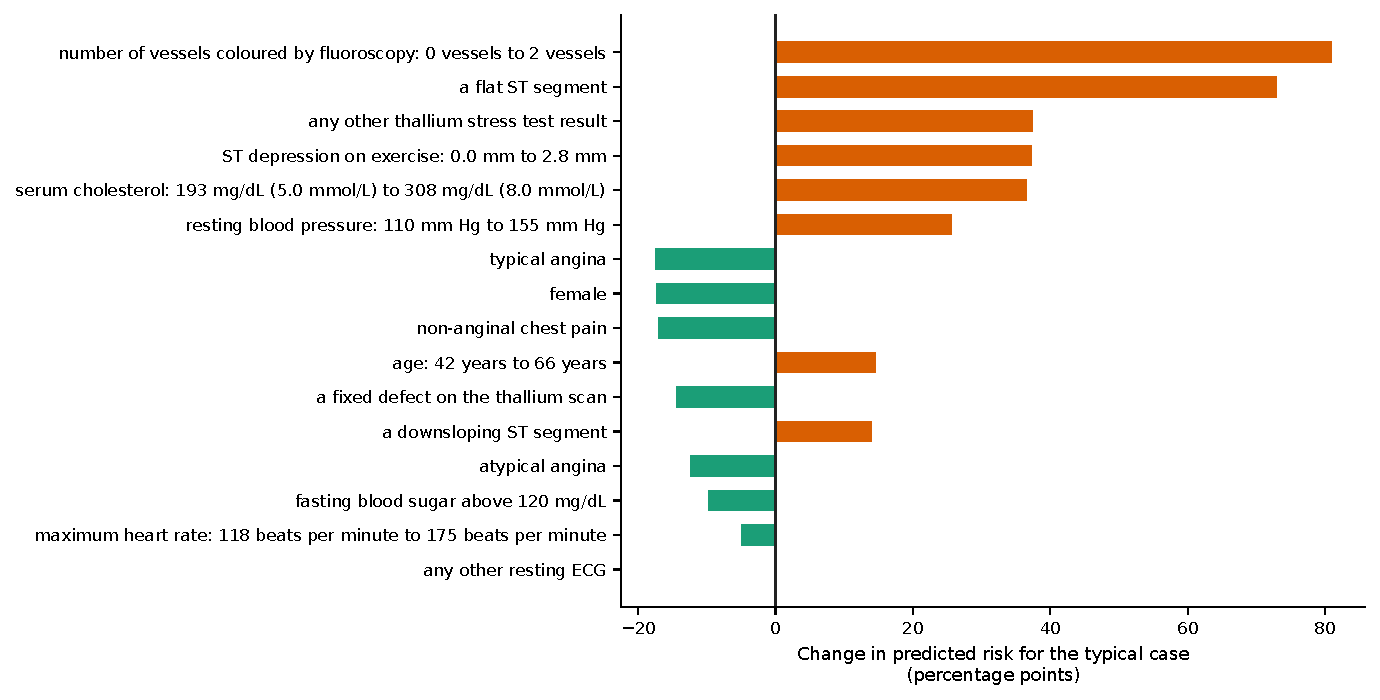
\includegraphics[width=\linewidth,height=0.88\textheight,keepaspectratio]{figures/heart-s1-c1/ann_34-effects.pdf}
\caption{The whole model: Each input's change in the predicted value for the typical case across the whole model, largest first (orange: raises it, teal: lowers it).}
\label{fig:hearts1c1:plot-ann34-0}
\end{figure}
\par\smallskip\noindent{\small \textbf{Dive deeper:} Typical angina with vessels (\ref{rd:ann33}); ST depression with a normal ECG (\ref{rd:ann31}); Vessels with flat ST segment (\ref{rd:ann29}); Non-anginal chest pain relay (\ref{rd:ann30}); Maximum heart rate (\ref{rd:ann32}). Technical detail: \ref{tech:ann34}.\par}
\subsubsection{Typical angina with vessels}\label{rd:ann33}
\noindent{\footnotesize Part of: The whole model (\ref{rd:ann34}).\par}
\noindent{\small Figure~\ref{fig:hearts1c1:parts-ann33} shows what feeds this part; Figure~\ref{fig:hearts1c1:units-ann33} its units and every connection into them (dashed boxes: connections from or to other parts, drawn in their own sections).\par}
\begin{figure}[H]\centering
\resizebox{!}{\ifdim\height>0.5\textheight 0.5\textheight\else\height\fi}{%
\resizebox{\ifdim\width>\linewidth\linewidth\else\width\fi}{!}{%
\begin{tikzpicture}[
  font=\sffamily\scriptsize, >={Stealth[length=1.6mm]},
  inp/.style={draw, rounded corners=1pt, fill=white, inner sep=1.5pt, minimum height=3.2mm, anchor=east},
  abox/.style={draw, thick, rounded corners=2pt, align=center, inner sep=3pt, minimum height=6mm, text width=42mm},
  outp/.style={draw, double, rounded corners=2pt, fill=white, align=center, inner sep=3pt, text width=24mm},
  agg/.style={draw=black!55},
]
\node[inp] (i0) at (0,0.375) {chest pain type};
\node[inp] (i1) at (0,-0.375) {number of vessels coloured by fluoroscopy};
\node[outp] (out) at (9.36,0) {Typical angina with vessels};
\begin{scope}[on background layer]
\draw[->, agg, thin, dashed] (i0.east) -- (out.west);
\draw[->, agg, thin, dashed] (i1.east) -- (out.west);
\end{scope}
\end{tikzpicture}}}%
\caption{Typical angina with vessels: what feeds it, one level down.}
\label{fig:hearts1c1:parts-ann33}
\end{figure}
\begin{figure}[H]\centering
\resizebox{\ifdim\width>\linewidth\linewidth\else\width\fi}{!}{%
\definecolor{netup}{HTML}{D95F02}\definecolor{netdown}{HTML}{1B9E77}\definecolor{netmixed}{HTML}{7F7F7F}%
\begin{tikzpicture}[
  font=\sffamily\scriptsize, >={Stealth[length=1.4mm]},
  inp/.style={draw, circle, fill=white, minimum size=3.2mm, inner sep=0pt},
  hid/.style={draw, circle, fill=white, minimum size=5.2mm, inner sep=0.5pt, font=\sffamily\tiny},
  exitbox/.style={draw, thick, rectangle, fill=white, align=center, text width=17mm, minimum height=5mm, inner sep=1.5pt, font=\sffamily\tiny},
  sumbox/.style={draw, thick, dashed, rectangle, fill=white, align=center, text width=17mm, minimum height=5mm, inner sep=1.5pt, font=\sffamily\tiny},
  outp/.style={draw, thick, regular polygon, regular polygon sides=6, fill=white, minimum size=10mm, inner sep=0pt, font=\sffamily\tiny, align=center},
  stub/.style={draw, dashed, rounded corners=2pt, fill=white, align=center, inner sep=2pt, font=\sffamily\tiny, text width=15mm},
  inlab/.style={font=\sffamily\tiny, align=center, text width=15mm, inner sep=1pt, fill=white, fill opacity=0.8, text opacity=1},
  wpos/.style={draw=NavyBlue}, wneg/.style={draw=BrickRed}, wagg/.style={draw=black!45, line width=1.2pt},
  wmix/.style={draw=Plum},
]
\node[hid] (n3210) at (2.7,3.25) {h7};
\node[hid] (n2245) at (2.7,1.9) {h5};
\node[inp, draw=netdown, very thick] (ninxxcpx1) at (1.8,0.0) {};
\path (ninxxcpx1.south) node[inlab, anchor=north] (labninxxcpx1) {typical angina $\downarrow$};
\node[inp, draw=netup, very thick] (ninxxca) at (3.6,0.0) {};
\path (ninxxca.south) node[inlab, anchor=north] (labninxxca) {vessels $\uparrow$};
\node[stub] (ntoxxthexmodelxoutput) at (2.7,4.8) {to the model output};
\begin{scope}[on background layer]
\node[fit=(n3210) (n2245) , inner sep=8pt, rounded corners=5pt, fill=BurntOrange!10, draw=BurntOrange!45] (clu0) {};
\draw[->, wpos, line width=0.57pt] (ninxxcpx1) -- (n3210);
\draw[->, wneg, line width=0.48pt] (n2245) -- (n3210);
\draw[->, wpos, line width=0.45pt] (ninxxca) -- (n2245);
\draw[->, wpos, line width=0.78pt] (n2245) -- (ntoxxthexmodelxoutput);
\draw[->, wneg, line width=0.54pt] (n3210) -- (ntoxxthexmodelxoutput);
\end{scope}
\node[font=\sffamily\scriptsize\bfseries, text=BurntOrange!55!black, anchor=south west, inner sep=1pt, fill=white, fill opacity=0.85, text opacity=1] at (clu0.north west) {Typical angina with vessels};
\end{tikzpicture}}%
\caption{Typical angina with vessels: its units and every connection into them. Blue: positive weight (raises the score); red: negative weight (lowers it); thicker: larger weight. Orange outline and up arrow: raises the final prediction; teal and down arrow: lowers it; grey and double arrow: depends.}
\label{fig:hearts1c1:units-ann33}
\end{figure}
\paragraph{Hypothesis.} This part lowers the predicted risk for typical angina and adds risk for each extra vessel coloured, about the same for each, with the vessels counting more for patients with typical angina.\,{\scriptsize\textcolor{NavyBlue}{[C31, C30, C32]}}
\paragraph{Evidence.} Through it, typical angina takes a typical patient's predicted risk from about 18\% to about 2\%, and each extra vessel adds about the same, from about 18\% at 0 to about 61\% at 2 vessels.\,{\scriptsize\textcolor{NavyBlue}{[C31, C30]}} Across the whole model, going from 0 to 2 vessels moves a typical patient from below 1\% to about 55\% with typical angina, each extra vessel adding about the same, and from about 18\% to about 99\% with any other chest pain type.\,{\scriptsize\textcolor{NavyBlue}{[C32]}} Its formula reproduces the part exactly on all 242 training patients.\,{\scriptsize\textcolor{NavyBlue}{[C33]}}
\par\noindent{\small Evidence plots: Figure~\ref{fig:hearts1c1:plot-ann33-0}, Figure~\ref{fig:hearts1c1:plot-ann33-1}, Figure~\ref{fig:hearts1c1:plot-ann33-2}, Figure~\ref{fig:hearts1c1:plot-ann33-3}, Figure~\ref{fig:hearts1c1:plot-ann33-4}, Figure~\ref{fig:hearts1c1:plot-ann33-5}.\par}
\par\noindent{\small Figure~\ref{fig:hearts1c1:plot-ann33-3} shows this part's own output, unit h5.\par}
\par\noindent{\small Figure~\ref{fig:hearts1c1:plot-ann33-4} shows this part's own output, unit h7.\par}
\begin{figure}[H]\centering
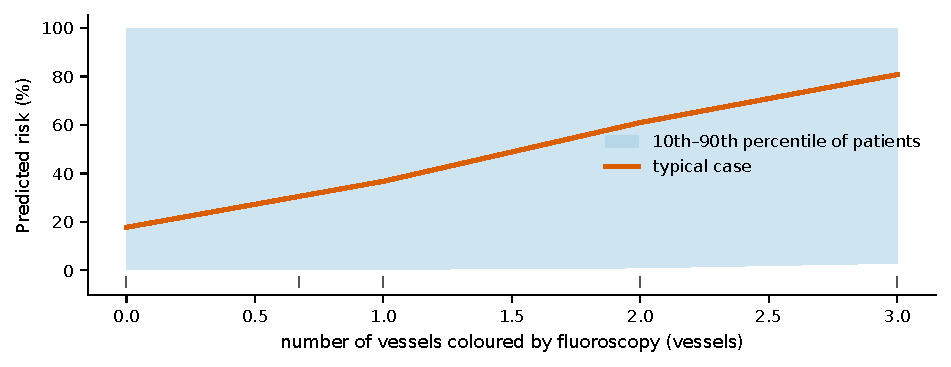
\includegraphics[width=\linewidth,height=0.88\textheight,keepaspectratio]{figures/heart-s1-c1/ann_33-response.pdf}
\caption{Typical angina with vessels: Response curves through this part: the typical case (bold), the 10th to 90th percentile of individual patients (band), the fold or step point (dashed) with its spread across them (grey), and the observed values (ticks).}
\label{fig:hearts1c1:plot-ann33-0}
\end{figure}
\begin{figure}[H]\centering
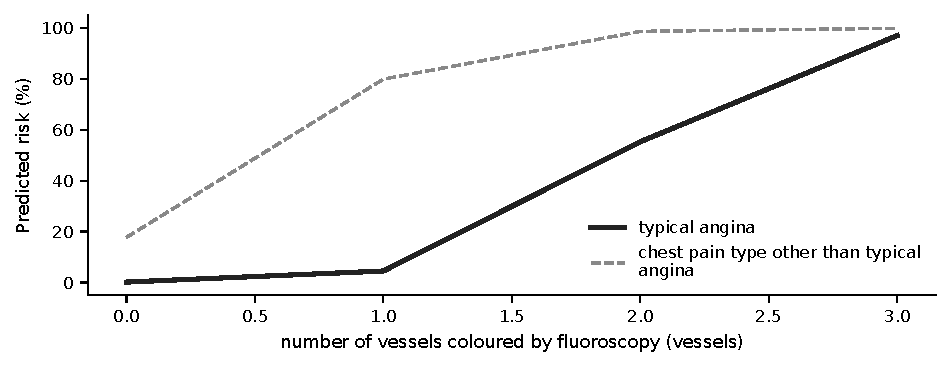
\includegraphics[width=\linewidth,height=0.88\textheight,keepaspectratio]{figures/heart-s1-c1/ann_33-interaction.pdf}
\caption{Typical angina with vessels: How the effect differs between groups: one curve per group, for the typical case of each group.}
\label{fig:hearts1c1:plot-ann33-1}
\end{figure}
\begin{figure}[H]\centering
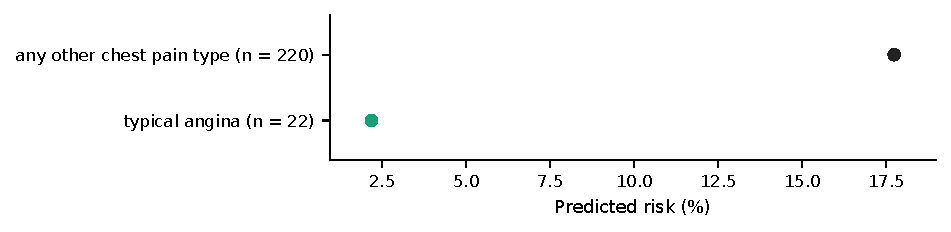
\includegraphics[width=\linewidth,height=0.88\textheight,keepaspectratio]{figures/heart-s1-c1/ann_33-categories-small.pdf}
\caption{Typical angina with vessels: The predicted value for the typical case at each level, through this part (n = training patients; grey: fewer than 20).}
\label{fig:hearts1c1:plot-ann33-2}
\end{figure}
\begin{figure}[H]\centering
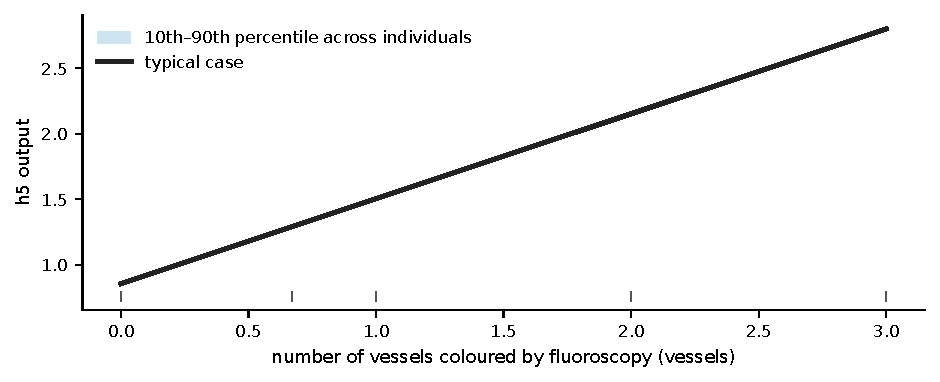
\includegraphics[width=\linewidth,height=0.88\textheight,keepaspectratio]{figures/heart-s1-c1/ann_33-partial-2245.pdf}
\caption{Typical angina with vessels: This part's own output, unit h5 (the output of 'Typical angina with vessels'), on its own scale (its activation), with every other input at the typical case; it is active for 242 of 242. Bold: the typical case; band: 10th to 90th percentile across individuals; ticks: the data.}
\label{fig:hearts1c1:plot-ann33-3}
\end{figure}
\begin{figure}[H]\centering
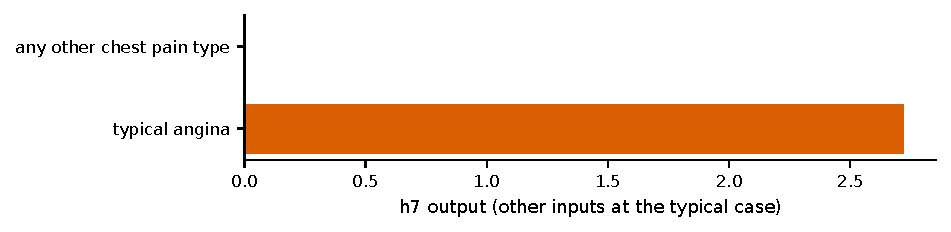
\includegraphics[width=\linewidth,height=0.88\textheight,keepaspectratio]{figures/heart-s1-c1/ann_33-partial-3210.pdf}
\caption{Typical angina with vessels: This part's own output, unit h7 (the output of 'Typical angina with vessels'), on its own scale (its activation), with every other input at the typical case; it is active for 22 of 242. Its output for each combination of the levels it reads.}
\label{fig:hearts1c1:plot-ann33-4}
\end{figure}
\begin{figure}[H]\centering
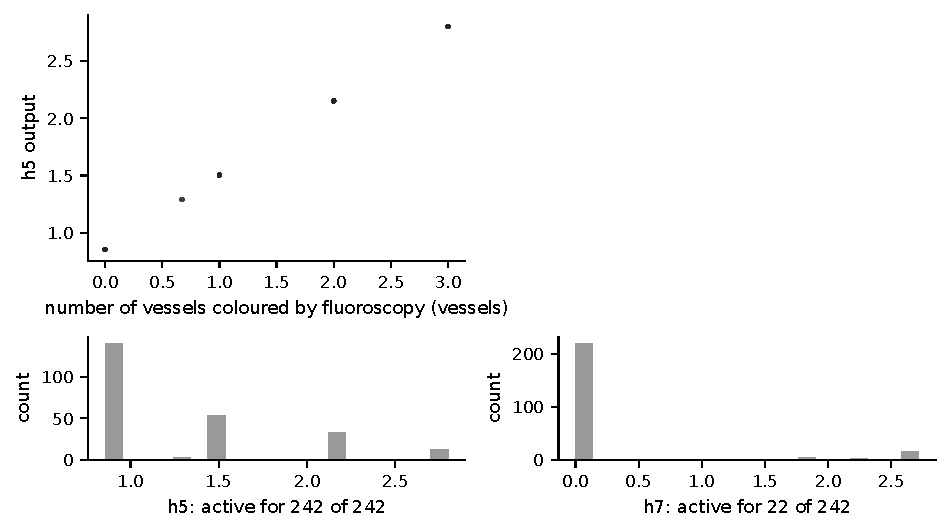
\includegraphics[width=\linewidth,height=0.88\textheight,keepaspectratio]{figures/heart-s1-c1/ann_33-units.pdf}
\caption{Typical angina with vessels: This part's hidden units: each unit's output against its main numeric input (top) and how often it is active (bottom).}
\label{fig:hearts1c1:plot-ann33-5}
\end{figure}
\par\smallskip\noindent{\small Technical detail: \ref{tech:ann33}.\par}
\subsubsection{ST depression with a normal ECG}\label{rd:ann31}
\noindent{\footnotesize Part of: The whole model (\ref{rd:ann34}).\par}
\noindent{\small Figure~\ref{fig:hearts1c1:parts-ann31} shows what feeds this part; Figure~\ref{fig:hearts1c1:units-ann31} its units and every connection into them (dashed boxes: connections from or to other parts, drawn in their own sections).\par}
\begin{figure}[H]\centering
\resizebox{!}{\ifdim\height>0.5\textheight 0.5\textheight\else\height\fi}{%
\resizebox{\ifdim\width>\linewidth\linewidth\else\width\fi}{!}{%
\begin{tikzpicture}[
  font=\sffamily\scriptsize, >={Stealth[length=1.6mm]},
  inp/.style={draw, rounded corners=1pt, fill=white, inner sep=1.5pt, minimum height=3.2mm, anchor=east},
  abox/.style={draw, thick, rounded corners=2pt, align=center, inner sep=3pt, minimum height=6mm, text width=42mm},
  outp/.style={draw, double, rounded corners=2pt, fill=white, align=center, inner sep=3pt, text width=24mm},
  agg/.style={draw=black!55},
]
\node[inp] (i0) at (0,0.375) {resting ECG};
\node[inp] (i1) at (0,-0.375) {ST depression on exercise};
\node[outp] (out) at (9.36,0) {ST depression with a normal ECG};
\begin{scope}[on background layer]
\draw[->, agg, thin, dashed] (i0.east) -- (out.west);
\draw[->, agg, thin, dashed] (i1.east) -- (out.west);
\end{scope}
\end{tikzpicture}}}%
\caption{ST depression with a normal ECG: what feeds it, one level down.}
\label{fig:hearts1c1:parts-ann31}
\end{figure}
\begin{figure}[H]\centering
\resizebox{\ifdim\width>\linewidth\linewidth\else\width\fi}{!}{%
\definecolor{netup}{HTML}{D95F02}\definecolor{netdown}{HTML}{1B9E77}\definecolor{netmixed}{HTML}{7F7F7F}%
\begin{tikzpicture}[
  font=\sffamily\scriptsize, >={Stealth[length=1.4mm]},
  inp/.style={draw, circle, fill=white, minimum size=3.2mm, inner sep=0pt},
  hid/.style={draw, circle, fill=white, minimum size=5.2mm, inner sep=0.5pt, font=\sffamily\tiny},
  exitbox/.style={draw, thick, rectangle, fill=white, align=center, text width=17mm, minimum height=5mm, inner sep=1.5pt, font=\sffamily\tiny},
  sumbox/.style={draw, thick, dashed, rectangle, fill=white, align=center, text width=17mm, minimum height=5mm, inner sep=1.5pt, font=\sffamily\tiny},
  outp/.style={draw, thick, regular polygon, regular polygon sides=6, fill=white, minimum size=10mm, inner sep=0pt, font=\sffamily\tiny, align=center},
  stub/.style={draw, dashed, rounded corners=2pt, fill=white, align=center, inner sep=2pt, font=\sffamily\tiny, text width=15mm},
  inlab/.style={font=\sffamily\tiny, align=center, text width=15mm, inner sep=1pt, fill=white, fill opacity=0.8, text opacity=1},
  wpos/.style={draw=NavyBlue}, wneg/.style={draw=BrickRed}, wagg/.style={draw=black!45, line width=1.2pt},
  wmix/.style={draw=Plum},
]
\node[exitbox] (n1801) at (3.1,1.9) {ST depression with a normal ECG $\uparrow$};
\node[inp, draw=netup, very thick] (ninxxrestecgx0) at (4.0,0.0) {};
\path (ninxxrestecgx0.south) node[inlab, anchor=north] (labninxxrestecgx0) {normal ECG $\uparrow$};
\node[inp, draw=netup, very thick] (ninxxoldpeak) at (2.2,0.0) {};
\path (ninxxoldpeak.south) node[inlab, anchor=north] (labninxxoldpeak) {ST depression $\uparrow$};
\node[stub] (ntoxxthexmodelxoutput) at (3.1,3.45) {to the model output};
\begin{scope}[on background layer]
\node[fit=(n1801) , inner sep=8pt, rounded corners=5pt, fill=ForestGreen!10, draw=ForestGreen!45] (clu0) {};
\draw[->, wpos, line width=0.79pt] (ninxxrestecgx0) -- (n1801);
\draw[->, wpos, line width=0.54pt] (ninxxoldpeak) -- (n1801);
\draw[->, wpos, line width=0.74pt] (n1801) -- (ntoxxthexmodelxoutput);
\end{scope}
\node[font=\sffamily\scriptsize\bfseries, text=ForestGreen!55!black, anchor=south west, inner sep=1pt, fill=white, fill opacity=0.85, text opacity=1] at (clu0.north west) {ST depression with a normal ECG};
\end{tikzpicture}}%
\caption{ST depression with a normal ECG: its units and every connection into them. Blue: positive weight (raises the score); red: negative weight (lowers it); thicker: larger weight. Orange outline and up arrow: raises the final prediction; teal and down arrow: lowers it; grey and double arrow: depends.}
\label{fig:hearts1c1:units-ann31}
\end{figure}
\paragraph{Hypothesis.} This part raises the predicted risk with ST depression on exercise, in an uneven way, only for patients with a normal resting ECG, once it rises above about 1.0 mm.\,{\scriptsize\textcolor{NavyBlue}{[C37, C36]}}
\paragraph{Evidence.} It acts on 42 of 242 training patients, nearly all with a normal resting ECG, 26 of whom had heart disease; for the typical patient it acts on, the predicted risk is about 98\% without it and about 99\% with it.\,{\scriptsize\textcolor{NavyBlue}{[C38]}} Through it, more ST depression raises the predicted risk only once it rises above about 1.0 mm, in an uneven way: for a typical patient with a normal resting ECG from about 13\% at 0 mm to about 63\% at 3.5 mm.\,{\scriptsize\textcolor{NavyBlue}{[C37]}} Going from 0 to 2.8 mm of ST depression moves a typical patient from about 18\% to about 55\% with a normal resting ECG, in an uneven way, and leaves it at about 18\% otherwise.\,{\scriptsize\textcolor{NavyBlue}{[C36]}} Its formula reproduces the part exactly on all 242 training patients.\,{\scriptsize\textcolor{NavyBlue}{[C39]}}
\par\noindent{\small Evidence plots: Figure~\ref{fig:hearts1c1:plot-ann31-0}, Figure~\ref{fig:hearts1c1:plot-ann31-1}, Figure~\ref{fig:hearts1c1:plot-ann31-2}, Figure~\ref{fig:hearts1c1:plot-ann31-3}, Figure~\ref{fig:hearts1c1:plot-ann31-4}.\par}
\par\noindent{\small Figure~\ref{fig:hearts1c1:plot-ann31-3} shows this part's own output, unit h3: it switches on at about 1.006 mm of ST depression on exercise, and is zero below.\par}
\begin{figure}[H]\centering
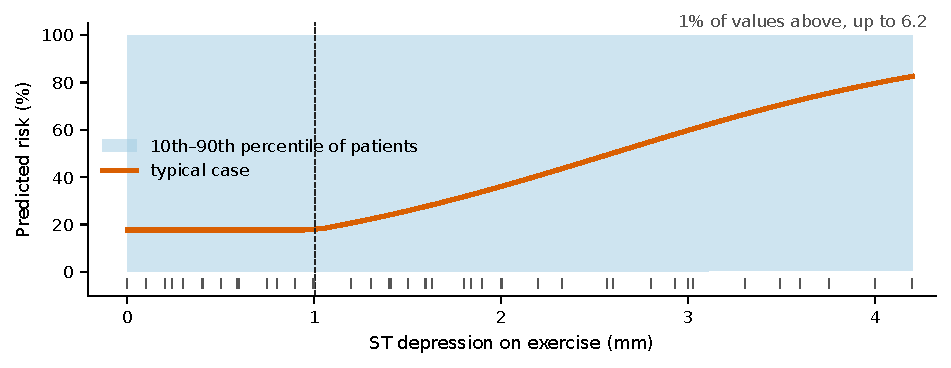
\includegraphics[width=\linewidth,height=0.88\textheight,keepaspectratio]{figures/heart-s1-c1/ann_31-response.pdf}
\caption{ST depression with a normal ECG: Response curves through this part: the typical case (bold), the 10th to 90th percentile of individual patients (band), the fold or step point (dashed) with its spread across them (grey), and the observed values (ticks).}
\label{fig:hearts1c1:plot-ann31-0}
\end{figure}
\begin{figure}[H]\centering
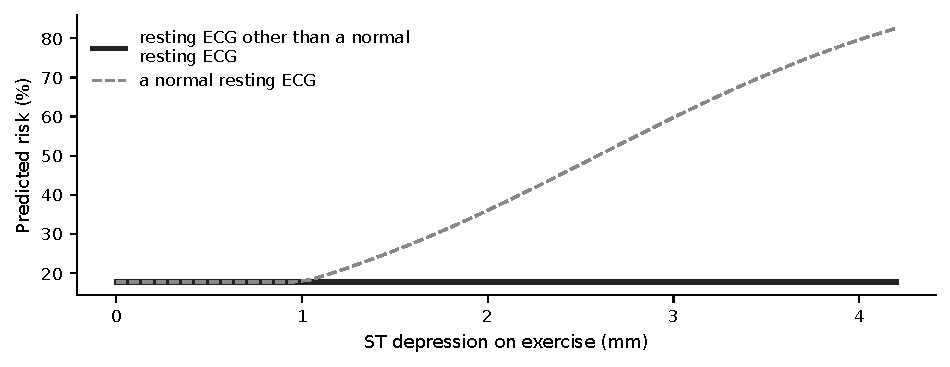
\includegraphics[width=\linewidth,height=0.88\textheight,keepaspectratio]{figures/heart-s1-c1/ann_31-interaction.pdf}
\caption{ST depression with a normal ECG: How the effect differs between groups: one curve per group, for the typical case of each group.}
\label{fig:hearts1c1:plot-ann31-1}
\end{figure}
\begin{figure}[H]\centering
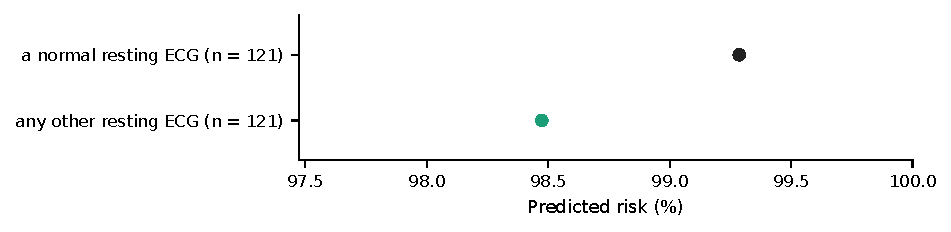
\includegraphics[width=\linewidth,height=0.88\textheight,keepaspectratio]{figures/heart-s1-c1/ann_31-categories-small.pdf}
\caption{ST depression with a normal ECG: The predicted value for the typical case at each level, through this part (n = training patients; grey: fewer than 20).}
\label{fig:hearts1c1:plot-ann31-2}
\end{figure}
\begin{figure}[H]\centering
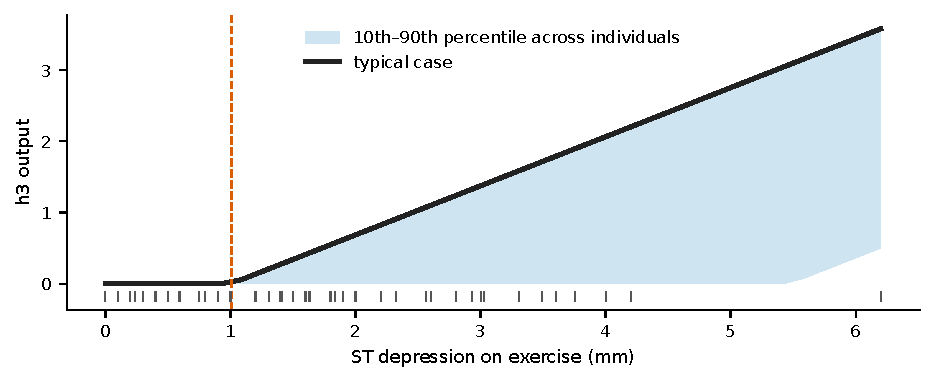
\includegraphics[width=\linewidth,height=0.88\textheight,keepaspectratio]{figures/heart-s1-c1/ann_31-partial-1801.pdf}
\caption{ST depression with a normal ECG: This part's own output, unit h3 (the output of 'ST depression with a normal ECG'), on its own scale (its activation), with every other input at the typical case; it is active for 42 of 242. Bold: the typical case; band: 10th to 90th percentile across individuals; dashed: where it switches on; ticks: the data.}
\label{fig:hearts1c1:plot-ann31-3}
\end{figure}
\begin{figure}[H]\centering
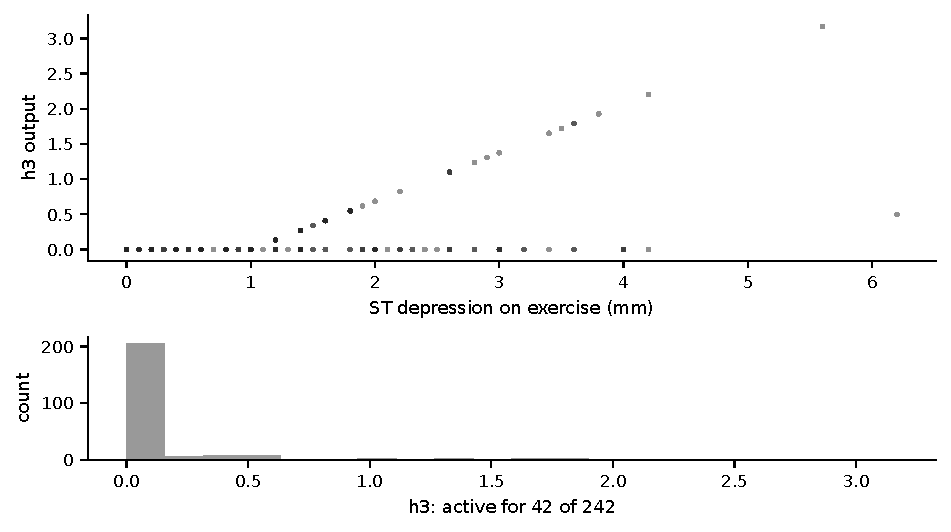
\includegraphics[width=\linewidth,height=0.88\textheight,keepaspectratio]{figures/heart-s1-c1/ann_31-units.pdf}
\caption{ST depression with a normal ECG: This part's hidden units: each unit's output against its main numeric input (top) and how often it is active (bottom).}
\label{fig:hearts1c1:plot-ann31-4}
\end{figure}
\par\smallskip\noindent{\small Technical detail: \ref{tech:ann31}.\par}
\subsubsection{Vessels with flat ST segment}\label{rd:ann29}
\noindent{\footnotesize Part of: The whole model (\ref{rd:ann34}).\par}
\noindent{\small Figure~\ref{fig:hearts1c1:parts-ann29} shows what feeds this part; Figure~\ref{fig:hearts1c1:units-ann29} its units and every connection into them (dashed boxes: connections from or to other parts, drawn in their own sections).\par}
\begin{figure}[H]\centering
\resizebox{!}{\ifdim\height>0.5\textheight 0.5\textheight\else\height\fi}{%
\resizebox{\ifdim\width>\linewidth\linewidth\else\width\fi}{!}{%
\begin{tikzpicture}[
  font=\sffamily\scriptsize, >={Stealth[length=1.6mm]},
  inp/.style={draw, rounded corners=1pt, fill=white, inner sep=1.5pt, minimum height=3.2mm, anchor=east},
  abox/.style={draw, thick, rounded corners=2pt, align=center, inner sep=3pt, minimum height=6mm, text width=42mm},
  outp/.style={draw, double, rounded corners=2pt, fill=white, align=center, inner sep=3pt, text width=24mm},
  agg/.style={draw=black!55},
]
\node[inp] (i0) at (0,0.375) {slope of the ST segment at peak exercise};
\node[inp] (i1) at (0,-0.375) {number of vessels coloured by fluoroscopy};
\node[outp] (out) at (9.36,0) {Vessels with flat ST segment};
\begin{scope}[on background layer]
\draw[->, agg, thin, dashed] (i0.east) -- (out.west);
\draw[->, agg, thin, dashed] (i1.east) -- (out.west);
\end{scope}
\end{tikzpicture}}}%
\caption{Vessels with flat ST segment: what feeds it, one level down.}
\label{fig:hearts1c1:parts-ann29}
\end{figure}
\begin{figure}[H]\centering
\resizebox{\ifdim\width>\linewidth\linewidth\else\width\fi}{!}{%
\definecolor{netup}{HTML}{D95F02}\definecolor{netdown}{HTML}{1B9E77}\definecolor{netmixed}{HTML}{7F7F7F}%
\begin{tikzpicture}[
  font=\sffamily\scriptsize, >={Stealth[length=1.4mm]},
  inp/.style={draw, circle, fill=white, minimum size=3.2mm, inner sep=0pt},
  hid/.style={draw, circle, fill=white, minimum size=5.2mm, inner sep=0.5pt, font=\sffamily\tiny},
  exitbox/.style={draw, thick, rectangle, fill=white, align=center, text width=17mm, minimum height=5mm, inner sep=1.5pt, font=\sffamily\tiny},
  sumbox/.style={draw, thick, dashed, rectangle, fill=white, align=center, text width=17mm, minimum height=5mm, inner sep=1.5pt, font=\sffamily\tiny},
  outp/.style={draw, thick, regular polygon, regular polygon sides=6, fill=white, minimum size=10mm, inner sep=0pt, font=\sffamily\tiny, align=center},
  stub/.style={draw, dashed, rounded corners=2pt, fill=white, align=center, inner sep=2pt, font=\sffamily\tiny, text width=15mm},
  inlab/.style={font=\sffamily\tiny, align=center, text width=15mm, inner sep=1pt, fill=white, fill opacity=0.8, text opacity=1},
  wpos/.style={draw=NavyBlue}, wneg/.style={draw=BrickRed}, wagg/.style={draw=black!45, line width=1.2pt},
  wmix/.style={draw=Plum},
]
\node[exitbox] (n664) at (2.8,1.9) {Vessels with flat ST segment $\uparrow$};
\node[inp, draw=netup, very thick] (ninxxca) at (3.7,0.0) {};
\path (ninxxca.south) node[inlab, anchor=north] (labninxxca) {vessels $\uparrow$};
\node[inp, draw=netup, very thick] (ninxxslopex2) at (1.9,0.0) {};
\path (ninxxslopex2.south) node[inlab, anchor=north] (labninxxslopex2) {flat ST $\uparrow$};
\node[stub] (ntoxxthexmodelxoutput) at (2.8,3.45) {to the model output};
\begin{scope}[on background layer]
\node[fit=(n664) , inner sep=8pt, rounded corners=5pt, fill=Orchid!10, draw=Orchid!45] (clu0) {};
\draw[->, wpos, line width=0.41pt] (ninxxca) -- (n664);
\draw[->, wpos, line width=0.31pt] (ninxxslopex2) -- (n664);
\draw[->, wpos, line width=0.57pt] (n664) -- (ntoxxthexmodelxoutput);
\end{scope}
\node[font=\sffamily\scriptsize\bfseries, text=Orchid!55!black, anchor=south west, inner sep=1pt, fill=white, fill opacity=0.85, text opacity=1] at (clu0.north west) {Vessels with flat ST segment};
\end{tikzpicture}}%
\caption{Vessels with flat ST segment: its units and every connection into them. Blue: positive weight (raises the score); red: negative weight (lowers it); thicker: larger weight. Orange outline and up arrow: raises the final prediction; teal and down arrow: lowers it; grey and double arrow: depends.}
\label{fig:hearts1c1:units-ann29}
\end{figure}
\paragraph{Hypothesis.} This part adds risk for each extra vessel coloured, about the same for each, and for a flat ST segment.\,{\scriptsize\textcolor{NavyBlue}{[C40, C41]}}
\paragraph{Evidence.} Through it, each extra vessel adds about the same, from about 18\% at 0 to about 36\% at 2 vessels for a typical patient, and a flat ST segment raises the risk from about 18\% to about 23\%.\,{\scriptsize\textcolor{NavyBlue}{[C40, C41]}} Its formula reproduces the part exactly on all 242 training patients.\,{\scriptsize\textcolor{NavyBlue}{[C42]}}
\par\noindent{\small Evidence plots: Figure~\ref{fig:hearts1c1:plot-ann29-0}, Figure~\ref{fig:hearts1c1:plot-ann29-1}, Figure~\ref{fig:hearts1c1:plot-ann29-2}.\par}
\begin{figure}[H]\centering
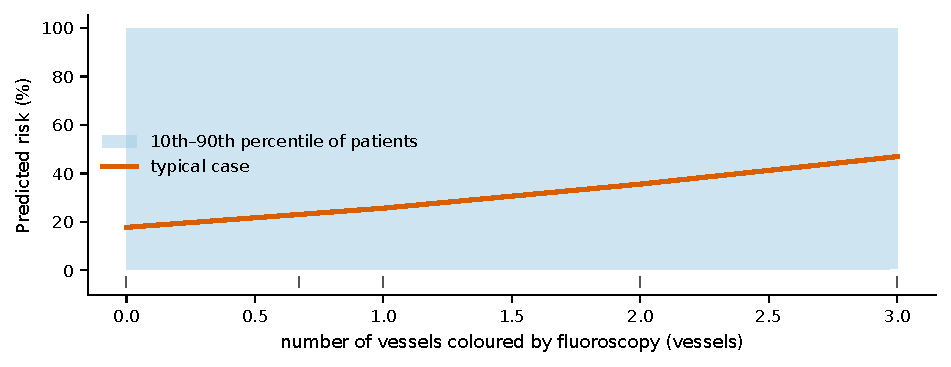
\includegraphics[width=\linewidth,height=0.88\textheight,keepaspectratio]{figures/heart-s1-c1/ann_29-response.pdf}
\caption{Vessels with flat ST segment: Response curves through this part: the typical case (bold), the 10th to 90th percentile of individual patients (band), the fold or step point (dashed) with its spread across them (grey), and the observed values (ticks).}
\label{fig:hearts1c1:plot-ann29-0}
\end{figure}
\begin{figure}[H]\centering
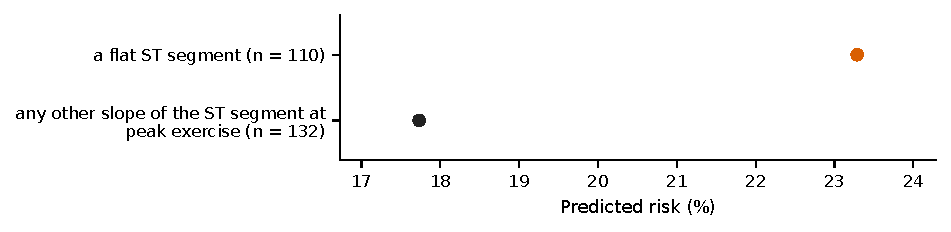
\includegraphics[width=\linewidth,height=0.88\textheight,keepaspectratio]{figures/heart-s1-c1/ann_29-categories-small.pdf}
\caption{Vessels with flat ST segment: The predicted value for the typical case at each level, through this part (n = training patients; grey: fewer than 20).}
\label{fig:hearts1c1:plot-ann29-1}
\end{figure}
\begin{figure}[H]\centering
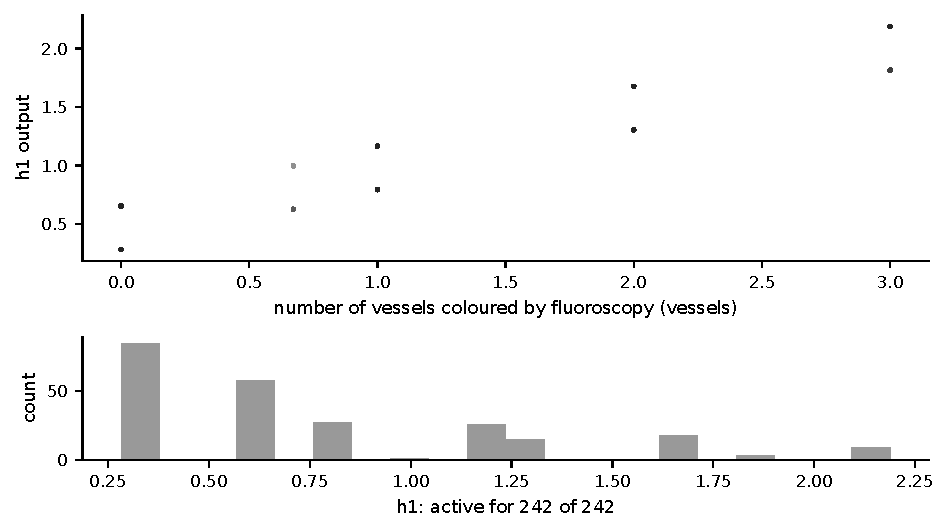
\includegraphics[width=\linewidth,height=0.88\textheight,keepaspectratio]{figures/heart-s1-c1/ann_29-units.pdf}
\caption{Vessels with flat ST segment: This part's hidden units: each unit's output against its main numeric input (top) and how often it is active (bottom).}
\label{fig:hearts1c1:plot-ann29-2}
\end{figure}
\par\smallskip\noindent{\small Technical detail: \ref{tech:ann29}.\par}
\subsubsection{Non-anginal chest pain relay}\label{rd:ann30}
\noindent{\footnotesize Part of: The whole model (\ref{rd:ann34}).\par}
\noindent{\small Figure~\ref{fig:hearts1c1:parts-ann30} shows what feeds this part; Figure~\ref{fig:hearts1c1:units-ann30} its units and every connection into them (dashed boxes: connections from or to other parts, drawn in their own sections).\par}
\begin{figure}[H]\centering
\resizebox{!}{\ifdim\height>0.5\textheight 0.5\textheight\else\height\fi}{%
\resizebox{\ifdim\width>\linewidth\linewidth\else\width\fi}{!}{%
\begin{tikzpicture}[
  font=\sffamily\scriptsize, >={Stealth[length=1.6mm]},
  inp/.style={draw, rounded corners=1pt, fill=white, inner sep=1.5pt, minimum height=3.2mm, anchor=east},
  abox/.style={draw, thick, rounded corners=2pt, align=center, inner sep=3pt, minimum height=6mm, text width=42mm},
  outp/.style={draw, double, rounded corners=2pt, fill=white, align=center, inner sep=3pt, text width=24mm},
  agg/.style={draw=black!55},
]
\node[inp] (i0) at (0,-0.0) {chest pain type};
\node[outp] (out) at (9.36,0) {Non-anginal chest pain relay};
\begin{scope}[on background layer]
\draw[->, agg, thin, dashed] (i0.east) -- (out.west);
\end{scope}
\end{tikzpicture}}}%
\caption{Non-anginal chest pain relay: what feeds it, one level down.}
\label{fig:hearts1c1:parts-ann30}
\end{figure}
\begin{figure}[H]\centering
\resizebox{\ifdim\width>\linewidth\linewidth\else\width\fi}{!}{%
\definecolor{netup}{HTML}{D95F02}\definecolor{netdown}{HTML}{1B9E77}\definecolor{netmixed}{HTML}{7F7F7F}%
\begin{tikzpicture}[
  font=\sffamily\scriptsize, >={Stealth[length=1.4mm]},
  inp/.style={draw, circle, fill=white, minimum size=3.2mm, inner sep=0pt},
  hid/.style={draw, circle, fill=white, minimum size=5.2mm, inner sep=0.5pt, font=\sffamily\tiny},
  exitbox/.style={draw, thick, rectangle, fill=white, align=center, text width=17mm, minimum height=5mm, inner sep=1.5pt, font=\sffamily\tiny},
  sumbox/.style={draw, thick, dashed, rectangle, fill=white, align=center, text width=17mm, minimum height=5mm, inner sep=1.5pt, font=\sffamily\tiny},
  outp/.style={draw, thick, regular polygon, regular polygon sides=6, fill=white, minimum size=10mm, inner sep=0pt, font=\sffamily\tiny, align=center},
  stub/.style={draw, dashed, rounded corners=2pt, fill=white, align=center, inner sep=2pt, font=\sffamily\tiny, text width=15mm},
  inlab/.style={font=\sffamily\tiny, align=center, text width=15mm, inner sep=1pt, fill=white, fill opacity=0.8, text opacity=1},
  wpos/.style={draw=NavyBlue}, wneg/.style={draw=BrickRed}, wagg/.style={draw=black!45, line width=1.2pt},
  wmix/.style={draw=Plum},
]
\node[exitbox] (n1173) at (2.8,1.9) {Non-anginal chest pain relay $\downarrow$};
\node[inp, draw=netdown, very thick] (ninxxcpx3) at (2.8,0.0) {};
\path (ninxxcpx3.south) node[inlab, anchor=north] (labninxxcpx3) {non-anginal pain $\downarrow$};
\node[stub] (ntoxxthexmodelxoutput) at (2.8,3.45) {to the model output};
\begin{scope}[on background layer]
\node[fit=(n1173) , inner sep=8pt, rounded corners=5pt, fill=Goldenrod!10, draw=Goldenrod!45] (clu0) {};
\draw[->, wpos, line width=0.37pt] (ninxxcpx3) -- (n1173);
\draw[->, wneg, line width=0.68pt] (n1173) -- (ntoxxthexmodelxoutput);
\end{scope}
\node[font=\sffamily\scriptsize\bfseries, text=Goldenrod!55!black, anchor=south west, inner sep=1pt, fill=white, fill opacity=0.85, text opacity=1] at (clu0.north west) {Non-anginal chest pain relay};
\end{tikzpicture}}%
\caption{Non-anginal chest pain relay: its units and every connection into them. Blue: positive weight (raises the score); red: negative weight (lowers it); thicker: larger weight. Orange outline and up arrow: raises the final prediction; teal and down arrow: lowers it; grey and double arrow: depends.}
\label{fig:hearts1c1:units-ann30}
\end{figure}
\paragraph{Hypothesis.} This part lowers the predicted risk for patients with non-anginal chest pain.\,{\scriptsize\textcolor{NavyBlue}{[C43]}}
\paragraph{Evidence.} Through it, non-anginal chest pain takes a typical patient's predicted risk from about 18\% to about 8\%.\,{\scriptsize\textcolor{NavyBlue}{[C43]}} Its formula reproduces the part exactly on all 242 training patients.\,{\scriptsize\textcolor{NavyBlue}{[C44]}}
\par\noindent{\small Evidence plots: Figure~\ref{fig:hearts1c1:plot-ann30-0}, Figure~\ref{fig:hearts1c1:plot-ann30-1}.\par}
\begin{figure}[H]\centering
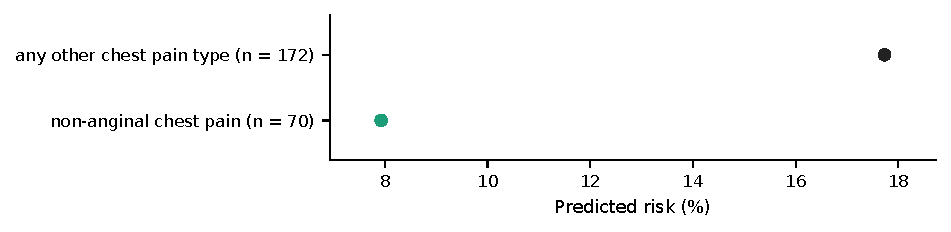
\includegraphics[width=\linewidth,height=0.88\textheight,keepaspectratio]{figures/heart-s1-c1/ann_30-categories-small.pdf}
\caption{Non-anginal chest pain relay: The predicted value for the typical case at each level, through this part (n = training patients; grey: fewer than 20).}
\label{fig:hearts1c1:plot-ann30-0}
\end{figure}
\begin{figure}[H]\centering
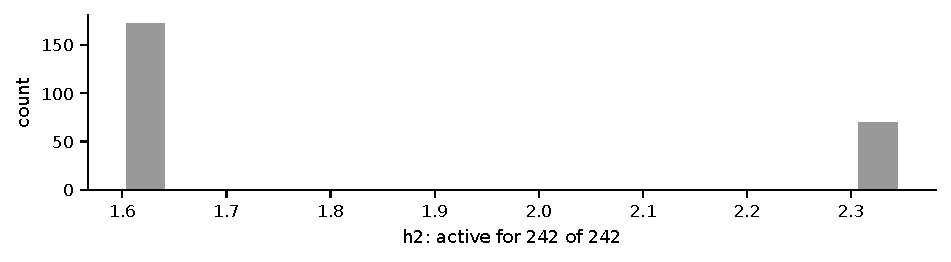
\includegraphics[width=\linewidth,height=0.88\textheight,keepaspectratio]{figures/heart-s1-c1/ann_30-units.pdf}
\caption{Non-anginal chest pain relay: This part's hidden units: each unit's output against its main numeric input (top) and how often it is active (bottom).}
\label{fig:hearts1c1:plot-ann30-1}
\end{figure}
\par\smallskip\noindent{\small Technical detail: \ref{tech:ann30}.\par}
\subsubsection{Maximum heart rate}\label{rd:ann32}
\noindent{\footnotesize Part of: The whole model (\ref{rd:ann34}).\par}
\noindent{\small Figure~\ref{fig:hearts1c1:parts-ann32} shows what feeds this part; Figure~\ref{fig:hearts1c1:units-ann32} its units and every connection into them (dashed boxes: connections from or to other parts, drawn in their own sections).\par}
\begin{figure}[H]\centering
\resizebox{!}{\ifdim\height>0.5\textheight 0.5\textheight\else\height\fi}{%
\resizebox{\ifdim\width>\linewidth\linewidth\else\width\fi}{!}{%
\begin{tikzpicture}[
  font=\sffamily\scriptsize, >={Stealth[length=1.6mm]},
  inp/.style={draw, rounded corners=1pt, fill=white, inner sep=1.5pt, minimum height=3.2mm, anchor=east},
  abox/.style={draw, thick, rounded corners=2pt, align=center, inner sep=3pt, minimum height=6mm, text width=42mm},
  outp/.style={draw, double, rounded corners=2pt, fill=white, align=center, inner sep=3pt, text width=24mm},
  agg/.style={draw=black!55},
]
\node[inp] (i0) at (0,-0.0) {maximum heart rate};
\node[outp] (out) at (9.36,0) {Maximum heart rate};
\begin{scope}[on background layer]
\draw[->, agg, thin, dashed] (i0.east) -- (out.west);
\end{scope}
\end{tikzpicture}}}%
\caption{Maximum heart rate: what feeds it, one level down.}
\label{fig:hearts1c1:parts-ann32}
\end{figure}
\begin{figure}[H]\centering
\resizebox{\ifdim\width>\linewidth\linewidth\else\width\fi}{!}{%
\definecolor{netup}{HTML}{D95F02}\definecolor{netdown}{HTML}{1B9E77}\definecolor{netmixed}{HTML}{7F7F7F}%
\begin{tikzpicture}[
  font=\sffamily\scriptsize, >={Stealth[length=1.4mm]},
  inp/.style={draw, circle, fill=white, minimum size=3.2mm, inner sep=0pt},
  hid/.style={draw, circle, fill=white, minimum size=5.2mm, inner sep=0.5pt, font=\sffamily\tiny},
  exitbox/.style={draw, thick, rectangle, fill=white, align=center, text width=17mm, minimum height=5mm, inner sep=1.5pt, font=\sffamily\tiny},
  sumbox/.style={draw, thick, dashed, rectangle, fill=white, align=center, text width=17mm, minimum height=5mm, inner sep=1.5pt, font=\sffamily\tiny},
  outp/.style={draw, thick, regular polygon, regular polygon sides=6, fill=white, minimum size=10mm, inner sep=0pt, font=\sffamily\tiny, align=center},
  stub/.style={draw, dashed, rounded corners=2pt, fill=white, align=center, inner sep=2pt, font=\sffamily\tiny, text width=15mm},
  inlab/.style={font=\sffamily\tiny, align=center, text width=15mm, inner sep=1pt, fill=white, fill opacity=0.8, text opacity=1},
  wpos/.style={draw=NavyBlue}, wneg/.style={draw=BrickRed}, wagg/.style={draw=black!45, line width=1.2pt},
  wmix/.style={draw=Plum},
]
\node[hid] (n2650) at (1.8,3.25) {h6};
\node[hid] (n2009) at (1.8,1.9) {h4};
\node[inp, draw=netdown, very thick] (ninxxthalach) at (1.8,0.0) {};
\path (ninxxthalach.south) node[inlab, anchor=north] (labninxxthalach) {max heart rate $\downarrow$};
\node[stub] (ntoxxthexmodelxoutput) at (1.8,4.8) {to the model output};
\begin{scope}[on background layer]
\node[fit=(n2650) (n2009) , inner sep=8pt, rounded corners=5pt, fill=Cerulean!10, draw=Cerulean!45] (clu0) {};
\draw[->, wpos, line width=0.59pt] (n2009) -- (n2650);
\draw[->, wpos, line width=0.54pt] (ninxxthalach) -- (n2009);
\draw[->, wneg, line width=0.30pt] (n2009) -- (ntoxxthexmodelxoutput);
\draw[->, wneg, line width=0.31pt] (n2650) -- (ntoxxthexmodelxoutput);
\end{scope}
\node[font=\sffamily\scriptsize\bfseries, text=Cerulean!55!black, anchor=south west, inner sep=1pt, fill=white, fill opacity=0.85, text opacity=1] at (clu0.north west) {Maximum heart rate};
\end{tikzpicture}}%
\caption{Maximum heart rate: its units and every connection into them. Blue: positive weight (raises the score); red: negative weight (lowers it); thicker: larger weight. Orange outline and up arrow: raises the final prediction; teal and down arrow: lowers it; grey and double arrow: depends.}
\label{fig:hearts1c1:units-ann32}
\end{figure}
\paragraph{Hypothesis.} This part lowers the predicted risk for a higher maximum heart rate: nothing until about 145 beats per minute, then steadily.\,{\scriptsize\textcolor{NavyBlue}{[C45, C46]}}
\paragraph{Evidence.} Through it, a higher maximum heart rate takes a typical patient from about 19\% at 71 to about 13\% at 182 beats per minute, with nothing until about 145 beats per minute, then steadily.\,{\scriptsize\textcolor{NavyBlue}{[C46]}} Its formula reproduces the part exactly on all 242 training patients.\,{\scriptsize\textcolor{NavyBlue}{[C47]}}
\par\noindent{\small Evidence plots: Figure~\ref{fig:hearts1c1:plot-ann32-0}, Figure~\ref{fig:hearts1c1:plot-ann32-1}, Figure~\ref{fig:hearts1c1:plot-ann32-2}, Figure~\ref{fig:hearts1c1:plot-ann32-3}.\par}
\par\noindent{\small Figure~\ref{fig:hearts1c1:plot-ann32-1} shows this part's own output, unit h4: it switches on at about 144.7 beats per minute of maximum heart rate, and is zero below.\par}
\par\noindent{\small Figure~\ref{fig:hearts1c1:plot-ann32-2} shows this part's own output, unit h6.\par}
\begin{figure}[H]\centering
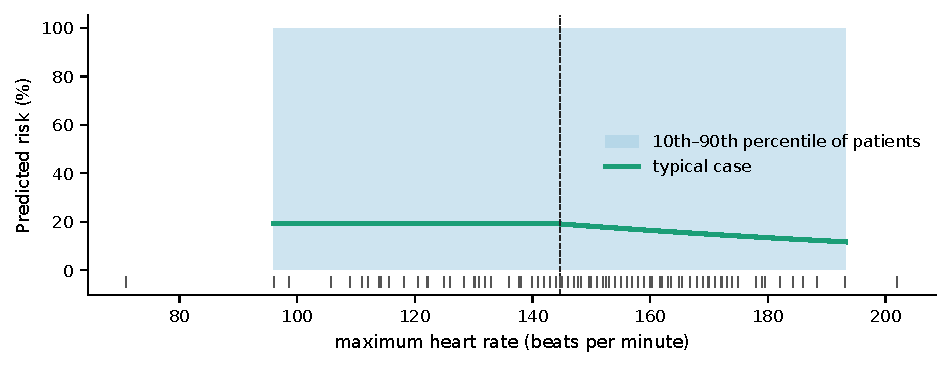
\includegraphics[width=\linewidth,height=0.88\textheight,keepaspectratio]{figures/heart-s1-c1/ann_32-response.pdf}
\caption{Maximum heart rate: Response curves through this part: the typical case (bold), the 10th to 90th percentile of individual patients (band), the fold or step point (dashed) with its spread across them (grey), and the observed values (ticks).}
\label{fig:hearts1c1:plot-ann32-0}
\end{figure}
\begin{figure}[H]\centering
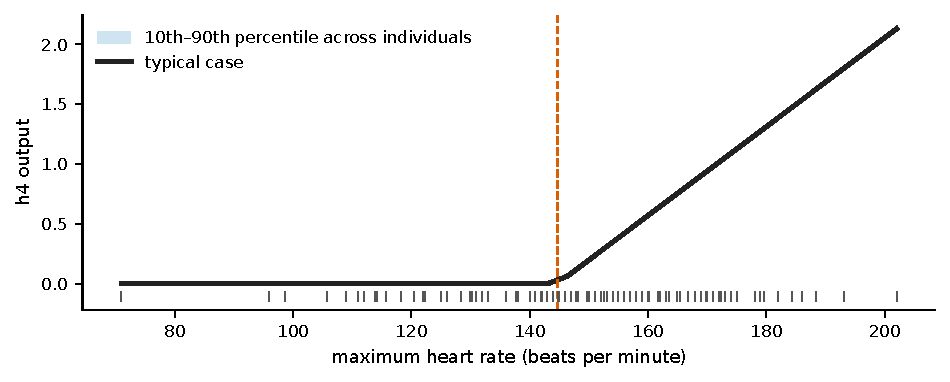
\includegraphics[width=\linewidth,height=0.88\textheight,keepaspectratio]{figures/heart-s1-c1/ann_32-partial-2009.pdf}
\caption{Maximum heart rate: This part's own output, unit h4 (the output of 'Maximum heart rate'), on its own scale (its activation), with every other input at the typical case; it is active for 155 of 242. Bold: the typical case; band: 10th to 90th percentile across individuals; dashed: where it switches on; ticks: the data.}
\label{fig:hearts1c1:plot-ann32-1}
\end{figure}
\begin{figure}[H]\centering
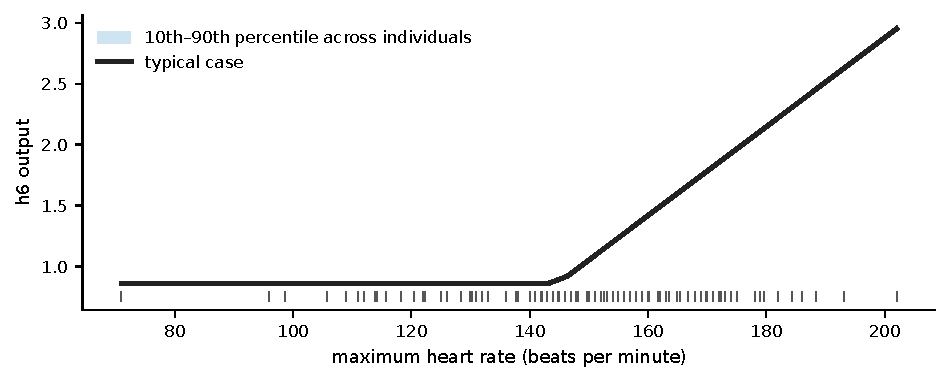
\includegraphics[width=\linewidth,height=0.88\textheight,keepaspectratio]{figures/heart-s1-c1/ann_32-partial-2650.pdf}
\caption{Maximum heart rate: This part's own output, unit h6 (the output of 'Maximum heart rate'), on its own scale (its activation), with every other input at the typical case; it is active for 242 of 242. Bold: the typical case; band: 10th to 90th percentile across individuals; ticks: the data.}
\label{fig:hearts1c1:plot-ann32-2}
\end{figure}
\begin{figure}[H]\centering
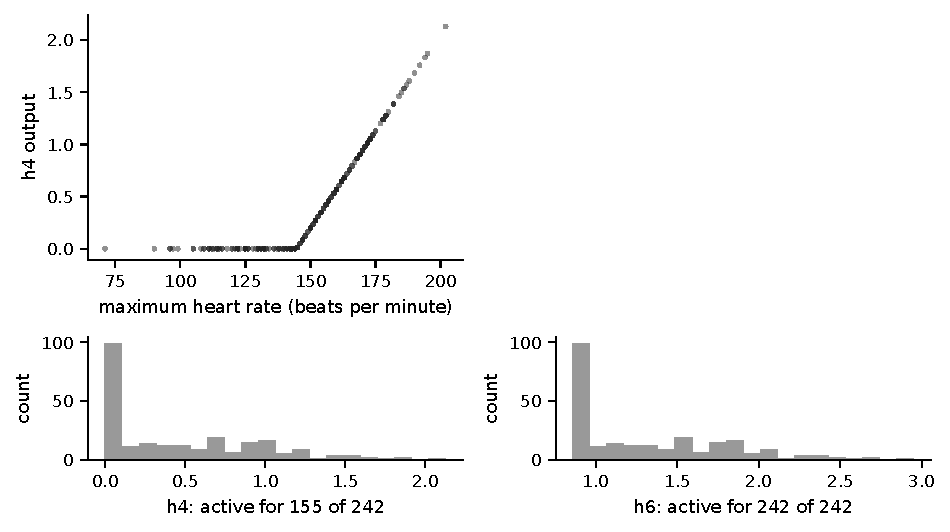
\includegraphics[width=\linewidth,height=0.88\textheight,keepaspectratio]{figures/heart-s1-c1/ann_32-units.pdf}
\caption{Maximum heart rate: This part's hidden units: each unit's output against its main numeric input (top) and how often it is active (bottom).}
\label{fig:hearts1c1:plot-ann32-3}
\end{figure}
\par\smallskip\noindent{\small Technical detail: \ref{tech:ann32}.\par}
\subsection{Not supported by the model}
\noindent{\small Every claim passed its checks.}
\clearpage\section*{Technical detail: heart-s1-c1}
\addcontentsline{toc}{section}{Technical detail: heart-s1-c1}
\noindent{\small The record behind each part: the original hypothesis, the closed form, and every claim with its estimate (log-odds and odds ratio), range across patients, n and test check.\par}
\renewcommand{\thesubsection}{T.\arabic{subsection}}\setcounter{subsection}{0}
\subsection{The whole model}\label{tech:ann34}
\noindent{\footnotesize Annotation ann\_\allowbreak{}34 (heart\_\allowbreak{}disease\_\allowbreak{}logit). Reads: age, sex, chest pain type, resting blood pressure, serum cholesterol, fasting blood sugar, resting ECG, maximum heart rate reached during the exercise test, exercise-induced angina, ST depression during exercise (compared with rest), slope of the ST segment at peak exercise, number of major vessels coloured by fluoroscopy, thallium stress test result.\par}
\paragraph{Original hypothesis (unchanged).} Hypothesis: the heart-disease logit is essentially a logistic regression. 13 direct input-$>$output edges (largest: sex:0 -1.87, slope:2 +1.72, ca +1.30, cp:4 +1.25, chol +0.93, thal:3 -0.87, thal:6 -0.86, trestbps +0.67, cp:2 +0.44, age +0.40, fbs:1 -0.32, slope:3 +0.20, thalach +0.002) are added to five children: ca\_\allowbreak{}slope2\_\allowbreak{}relay and the 2245 relay (raise the effective ca weight to 2.60 per SD), cp3\_\allowbreak{}relay (non-anginal pain lowers risk), st\_\allowbreak{}depression\_\allowbreak{}normal\_\allowbreak{}ecg\_\allowbreak{}gate (ST depression raises risk only with a normal resting ECG), typical\_\allowbreak{}angina\_\allowbreak{}ca\_\allowbreak{}switch's 3210 (typical angina lowers risk, less with more vessels) and max\_\allowbreak{}heart\_\allowbreak{}rate\_\allowbreak{}hinge (small). Nine inputs are unconnected (sex:1, fbs:0, restecg:1, restecg:2, exang:0, exang:1, slope:1, thal:4, thal:7): exercise-induced angina is ignored. Evidence (train, n=242): AUC 0.9392; all hidden units replaced by their best linear fits 0.9355 (= L2 logistic regression 0.9355); all ReLUs as identity 0.9078; all hidden mean-ablated 0.9241. The gain over linear (+0.0037) comes from the ECG/ST gate (+0.0034 restored alone), the heart-rate hinge (+0.0008) and the typical-angina switch (+0.0003); the relays contribute none. Direct edges carry logit SD 4.25 of 5.63.
\paragraph{Closed form.} Read through its parts (their formulas are in their own sections).
\paragraph{Split inputs.} To annotate the parts, the explanation split these inputs into copies (a refactoring step that does not change what the model computes); the diagrams draw each input once: vessels (3 copies); flat ST (2 copies); max heart rate (2 copies).
\paragraph{Evidence table} (next page, landscape).
\begin{landscape}
{\scriptsize\setlength{\tabcolsep}{3pt}\renewcommand{\arraystretch}{1.15}
\rowcolors{2}{black!6}{white}
\begin{longtable}{@{}l>{\raggedright\arraybackslash}p{0.36\linewidth}>{\raggedright\arraybackslash}p{0.14\linewidth}rrr>{\raggedright\arraybackslash}p{0.06\linewidth}>{\raggedright\arraybackslash}p{0.17\linewidth}c@{}}
\toprule\rowcolor{white}
ID & What is checked & Risk, typical patient & Log-odds & OR & Range (p10--p90) & n & Test check & OK \\
\midrule\endfirsthead
\toprule\rowcolor{white}
ID & What is checked & Risk, typical patient & Log-odds & OR & Range (p10--p90) & n & Test check & OK \\
\midrule\endhead
\bottomrule\endfoot
C01 & direction: number of vessels coloured by fluoroscopy: 0 vessels to 2 vessels (whole model) \newline{\itshape shape: steady (equal steps); 100\% of patients same; verified; risk saturates near 100\%} & 18\% to 99\% & 5.89 & 362 & 5.83 to 5.83 & 242 & unclear; AUC gain 0.041 [-0.032, 0.123] & \textcolor{OliveGreen}{yes} \\
C02 & direction: slope of the ST segment at peak exercise: an upsloping ST segment to a flat ST segment (whole model) \newline{\itshape shape: categorical; highest to lowest: a flat ST segment, a downsloping ST segment, an upsloping ST segment} & 18\% to 91\% & 3.81 & 44.9 & 3.81 to 3.81 & 115, 110 & disagrees; AUC gain -0.011 [-0.065, 0.036] & \textcolor{OliveGreen}{yes} \\
C03 & direction: slope of the ST segment at peak exercise: an upsloping ST segment to a flat ST segment (direct contribution only, not through any part) \newline{\itshape shape: categorical; highest to lowest: a flat ST segment, a downsloping ST segment, an upsloping ST segment} & 18\% to 87\% & 3.46 & 31.9 & 3.46 to 3.46 & 115, 110 & disagrees; AUC gain -0.012 [-0.059, 0.030] & \textcolor{OliveGreen}{yes} \\
C04 & direction: number of vessels coloured by fluoroscopy: 0 vessels to 2 vessels (direct contribution only, not through any part) \newline{\itshape shape: steady (equal steps); 100\% of patients same; verified} & 18\% to 80\% & 2.91 & 18.3 & 2.91 to 2.91 & 242 & disagrees; AUC gain -0.001 [-0.039, 0.032] & \textcolor{OliveGreen}{yes} \\
C05 & direction: thallium stress test result: a normal thallium scan to thallium stress test result other than a normal thallium scan, a fixed defect on the thallium scan (whole model) \newline{\itshape shape: categorical; highest to lowest: thallium stress test result other than a normal thallium scan, a fixed defect on the thallium scan, a normal thallium scan, a fixed defect on the thallium scan} & 18\% to 55\% & 1.74 & 5.71 & 1.74 to 1.74 & 135, 92 & unclear; AUC gain 0.012 [-0.017, 0.044] & \textcolor{OliveGreen}{yes} \\
C06 & direction: ST depression on exercise: 0.0 mm to 2.8 mm (whole model) \newline{\itshape shape: hinge at 1.0 mm; 100\% of patients same; fallback; matches the fold at 1.0 mm} & 18\% to 55\% & 0.87 & 2.38 & 0.00 to 1.74 & 242 & unclear; AUC gain 0.005 [-0.005, 0.022] & \textcolor{OliveGreen}{yes} \\
C07 & direction: serum cholesterol: 193 mg/dL (5.0 mmol/L) to 308 mg/dL (8.0 mmol/L) (whole model) \newline{\itshape shape: steady; 100\% of patients same; verified} & 8\% to 45\% & 2.22 & 9.23 & 2.22 to 2.22 & 242 & disagrees; AUC gain -0.022 [-0.066, 0.011] & \textcolor{OliveGreen}{yes} \\
C08 & direction: resting blood pressure: 110 mm Hg to 155 mm Hg (whole model) \newline{\itshape shape: steady; 100\% of patients same; verified} & 9\% to 35\% & 1.65 & 5.20 & 1.65 to 1.65 & 242 & unclear; AUC gain 0.000 [-0.022, 0.020] & \textcolor{OliveGreen}{yes} \\
C09 & direction: chest pain type: no chest pain (asymptomatic) to typical angina (whole model) \newline{\itshape shape: categorical; highest to lowest: no chest pain (asymptomatic), atypical angina, non-anginal chest pain, typical angina} & 18\% to $<$1\% & -4.55 & 0.01 & -4.78 to -4.08 & 108, 22 & agrees; AUC gain 0.041 [0.003, 0.083] & \textcolor{OliveGreen}{yes} \\
C10 & direction: sex: male to female (whole model) \newline{\itshape shape: categorical; highest to lowest: male, female} & 18\% to $<$1\% & -3.94 & 0.02 & -3.94 to -3.94 & 159, 83 & unclear; AUC gain 0.023 [-0.014, 0.068] & \textcolor{OliveGreen}{yes} \\
C11 & direction: chest pain type: no chest pain (asymptomatic) to non-anginal chest pain (whole model) \newline{\itshape shape: categorical; highest to lowest: no chest pain (asymptomatic), atypical angina, non-anginal chest pain, typical angina} & 18\% to 1\% & -3.43 & 0.03 & -3.43 to -3.43 & 108, 70 & agrees; AUC gain 0.041 [0.003, 0.083] & \textcolor{OliveGreen}{yes} \\
C12 & direction: chest pain type: no chest pain (asymptomatic) to chest pain type other than atypical angina, no chest pain (asymptomatic) (direct contribution only, not through any part) \newline{\itshape shape: categorical; highest to lowest: no chest pain (asymptomatic), atypical angina, chest pain type other than atypical angina, no chest pain (asymptomatic)} & 18\% to 2\% & -2.51 & 0.08 & -2.51 to -2.51 & 108, 92 & agrees; AUC gain 0.037 [0.006, 0.074] & \textcolor{OliveGreen}{yes} \\
C13 & direction: age: 42 years to 66 years (whole model) \newline{\itshape shape: steady; 100\% of patients same; verified} & 10\% to 25\% & 1.05 & 2.87 & 1.05 to 1.05 & 242 & disagrees; AUC gain -0.008 [-0.018, 0.001] & \textcolor{OliveGreen}{yes} \\
C14 & direction: thallium stress test result: a normal thallium scan to a fixed defect on the thallium scan (whole model) \newline{\itshape shape: categorical; highest to lowest: thallium stress test result other than a normal thallium scan, a fixed defect on the thallium scan, a normal thallium scan, a fixed defect on the thallium scan} & 18\% to 3\% & -1.83 & 0.16 & -1.83 to -1.83 & 135, 15 (small n) & unclear; AUC gain 0.012 [-0.017, 0.044] & \textcolor{OliveGreen}{yes} \\
C15 & direction: slope of the ST segment at peak exercise: an upsloping ST segment to a downsloping ST segment (direct contribution only, not through any part) \newline{\itshape shape: categorical; highest to lowest: a flat ST segment, a downsloping ST segment, an upsloping ST segment} & 18\% to 32\% & 0.77 & 2.16 & 0.77 to 0.77 & 115, 17 (small n) & disagrees; AUC gain -0.012 [-0.059, 0.030] & \textcolor{OliveGreen}{yes} \\
C16 & direction: slope of the ST segment at peak exercise: an upsloping ST segment to a downsloping ST segment (whole model) \newline{\itshape shape: categorical; highest to lowest: a flat ST segment, a downsloping ST segment, an upsloping ST segment} & 18\% to 32\% & 0.77 & 2.16 & 0.77 to 0.77 & 115, 17 (small n) & disagrees; AUC gain -0.011 [-0.065, 0.036] & \textcolor{OliveGreen}{yes} \\
C17 & direction: chest pain type: no chest pain (asymptomatic) to atypical angina (direct contribution only, not through any part) \newline{\itshape shape: categorical; highest to lowest: no chest pain (asymptomatic), atypical angina, chest pain type other than atypical angina, no chest pain (asymptomatic)} & 18\% to 5\% & -1.34 & 0.26 & -1.34 to -1.34 & 108, 42 & agrees; AUC gain 0.037 [0.006, 0.074] & \textcolor{OliveGreen}{yes} \\
C18 & direction: chest pain type: no chest pain (asymptomatic) to atypical angina (whole model) \newline{\itshape shape: categorical; highest to lowest: no chest pain (asymptomatic), atypical angina, non-anginal chest pain, typical angina} & 18\% to 5\% & -1.34 & 0.26 & -1.34 to -1.34 & 108, 42 & agrees; AUC gain 0.041 [0.003, 0.083] & \textcolor{OliveGreen}{yes} \\
C19 & direction: fasting blood sugar: fasting blood sugar of 120 mg/dL or less to fasting blood sugar above 120 mg/dL (whole model) \newline{\itshape shape: categorical; highest to lowest: fasting blood sugar of 120 mg/dL or less, fasting blood sugar above 120 mg/dL} & 18\% to 8\% & -0.92 & 0.40 & -0.92 to -0.92 & 209, 33 & disagrees; AUC gain -0.001 [-0.010, 0.009] & \textcolor{OliveGreen}{yes} \\
C20 & direction: maximum heart rate: 118 beats per minute to 175 beats per minute (whole model) \newline{\itshape shape: hinge at 145 beats per minute; 100\% of patients same; verified; matches the fold at 145 beats per minute} & 19\% to 14\% & -0.36 & 0.70 & -0.36 to -0.36 & 242 & unclear; AUC gain 0.002 [0.000, 0.009] & \textcolor{OliveGreen}{yes} \\
C21 & direction: maximum heart rate: 118 beats per minute to 175 beats per minute (direct contribution only, not through any part) \newline{\itshape shape: flat; 100\% of patients same; verified} & 18\% to 18\% & 0.005 & 1.00 & 0.005 to 0.005 & 242 & unclear; AUC gain 0.000 [0.000, 0.000] & \textcolor{OliveGreen}{yes} \\
C22 & direction: resting ECG: a normal resting ECG to resting ECG other than a normal resting ECG (whole model) \newline{\itshape shape: categorical; highest to lowest: a normal resting ECG, resting ECG other than a normal resting ECG} & 18\% to 18\% & -0.46 & 0.63 & -1.74 to 0.00 & 121, 121 & disagrees; AUC gain -0.008 [-0.021, 0.000] & \textcolor{OliveGreen}{yes} \\
C23 & magnitude: number of vessels coloured by fluoroscopy: 0 vessels to 2 vessels, typical patient \newline{\itshape shape: steady (equal steps); 100\% of patients same; verified; risk saturates near 100\%} & 18\% to 99\% & 5.83 & 340 &  & 242 & unclear; AUC gain 0.041 [-0.032, 0.123] & \textcolor{OliveGreen}{yes} \\
C24 & magnitude: slope of the ST segment at peak exercise: an upsloping ST segment to a flat ST segment, typical patient \newline{\itshape shape: categorical; highest to lowest: a flat ST segment, a downsloping ST segment, an upsloping ST segment} & 18\% to 91\% & 3.81 & 44.9 &  & 115, 110 & disagrees; AUC gain -0.011 [-0.065, 0.036] & \textcolor{OliveGreen}{yes} \\
C25 & magnitude: thallium stress test result: a normal thallium scan to thallium stress test result other than a normal thallium scan, a fixed defect on the thallium scan, typical patient \newline{\itshape shape: categorical; highest to lowest: thallium stress test result other than a normal thallium scan, a fixed defect on the thallium scan, a normal thallium scan, a fixed defect on the thallium scan} & 18\% to 55\% & 1.74 & 5.71 &  & 135, 92 & unclear; AUC gain 0.012 [-0.017, 0.044] & \textcolor{OliveGreen}{yes} \\
C26 & magnitude: ST depression on exercise: 0.0 mm to 2.8 mm, typical patient \newline{\itshape shape: hinge at 1.0 mm; 100\% of patients same; fallback; matches the fold at 1.0 mm} & 18\% to 55\% & 1.74 & 5.68 &  & 242 & unclear; AUC gain 0.005 [-0.005, 0.022] & \textcolor{OliveGreen}{yes} \\
C27 & magnitude: serum cholesterol: 193 mg/dL (5.0 mmol/L) to 308 mg/dL (8.0 mmol/L), typical patient \newline{\itshape shape: steady; 100\% of patients same; verified} & 8\% to 45\% & 2.22 & 9.23 &  & 242 & disagrees; AUC gain -0.022 [-0.066, 0.011] & \textcolor{OliveGreen}{yes} \\
C28 & null: model ignores exercise-induced angina (exact rule) &  & 0.00 &  &  & 242 & train only & \textcolor{OliveGreen}{yes} \\
C29 & structure: made of ca\_\allowbreak{}slope2\_\allowbreak{}relay, cp3\_\allowbreak{}relay, st\_\allowbreak{}depression\_\allowbreak{}normal\_\allowbreak{}ecg\_\allowbreak{}gate,\allowbreak{} max\_\allowbreak{}heart\_\allowbreak{}rate\_\allowbreak{}hinge,\allowbreak{} typical\_\allowbreak{}angina\_\allowbreak{}ca\_\allowbreak{}switch and inputs age, sex, cp, trestbps, chol, fbs, thalach, slope, ca, thal; added &  &  &  &  & 242 & train only & \textcolor{OliveGreen}{yes} \\
\end{longtable}}
\end{landscape}
\subsection{Typical angina with vessels}\label{tech:ann33}
\noindent{\footnotesize Annotation ann\_\allowbreak{}33 (typical\_\allowbreak{}angina\_\allowbreak{}ca\_\allowbreak{}switch). Reads: chest pain type, number of major vessels coloured by fluoroscopy.\par}
\paragraph{Original hypothesis (unchanged).} Hypothesis: (i) node 2245 = ReLU(0.578 ca + 1.276) is an always-on ca relay adding +0.88 logit per SD of ca (output weight 1.528); (ii) node 3210 = ReLU(0.901 cp:1 - 0.644*2245 + 0.420) is a typical-angina switch: it is on only for cp:1 patients and then lowers the logit by 0.833 x its activation, from about -2.26 at the lowest ca (-0.73 SD) to about -1.22 at the highest ca (2.64 SD). So typical angina lowers predicted risk, and the reduction shrinks with more narrowed vessels. Evidence (train, n=242): 2245 never clips (0.86..2.80); 3210 active for all 22 cp:1 patients and none of the 220 others. Mean ablation AUC 2245 0.9339, 3210 0.9354; linear replacement 0.9392 / 0.9391 (3210 is a cp:1 switch whose within-group response is linear in ca).
\paragraph{Closed form} {\footnotesize(weights and biases at 3 significant figures; largest difference from the part on the training patients 0.0).}
{\small\begingroup\allowdisplaybreaks
\begin{align*}
y_{0} &= \operatorname{relu}\bigl(1.28 + 0.578 x_{ca\_c}\bigr) \\
y_{1} &= \operatorname{relu}\bigl(0.42 + 0.901 x_{cp:1} - 0.644 \operatorname{relu}\bigl(1.28 \\
&\qquad + 0.578 x_{ca\_c}\bigr)\bigr)
\end{align*}\endgroup}

\paragraph{Evidence table} (next page, landscape).
\begin{landscape}
{\scriptsize\setlength{\tabcolsep}{3pt}\renewcommand{\arraystretch}{1.15}
\rowcolors{2}{black!6}{white}
\begin{longtable}{@{}l>{\raggedright\arraybackslash}p{0.36\linewidth}>{\raggedright\arraybackslash}p{0.14\linewidth}rrr>{\raggedright\arraybackslash}p{0.06\linewidth}>{\raggedright\arraybackslash}p{0.17\linewidth}c@{}}
\toprule\rowcolor{white}
ID & What is checked & Risk, typical patient & Log-odds & OR & Range (p10--p90) & n & Test check & OK \\
\midrule\endfirsthead
\toprule\rowcolor{white}
ID & What is checked & Risk, typical patient & Log-odds & OR & Range (p10--p90) & n & Test check & OK \\
\midrule\endhead
\bottomrule\endfoot
C30 & direction: number of vessels coloured by fluoroscopy: 0 vessels to 2 vessels (through this part) \newline{\itshape shape: steady (equal steps); 100\% of patients same; verified} & 18\% to 61\% & 2.04 & 7.73 & 1.98 to 1.98 & 242 & disagrees; AUC gain -0.003 [-0.032, 0.019] & \textcolor{OliveGreen}{yes} \\
C31 & direction: chest pain type: chest pain type other than typical angina to typical angina (through this part) \newline{\itshape shape: categorical; highest to lowest: chest pain type other than typical angina, typical angina} & 18\% to 2\% & -2.04 & 0.13 & -2.26 to -1.57 & 220, 22 & unclear; AUC gain 0.001 [-0.005, 0.008] & \textcolor{OliveGreen}{yes} \\
C32 & interaction: effect of number of vessels coloured by fluoroscopy (0 vessels to 2 vessels) by chest pain type: typical angina minus chest pain type other than typical angina; stronger in typical angina \newline{\itshape shape: steady (equal steps); 100\% of patients same; verified; risk saturates near 0\%} & typical angina: $<$1\% to 55\%; chest pain type other than typical angina: 18\% to 99\% & 0.70 & 2.00 &  & 22, 220 & agrees; AUC gain 0.001 [-0.005, 0.008] & \textcolor{OliveGreen}{yes} \\
C33 & structure: its formula reproduces it on 242 training patients (largest difference 0.0) &  & 0.00 &  &  & 242 & train only & \textcolor{OliveGreen}{yes} \\
\end{longtable}}
\end{landscape}
\subsection{ST depression with a normal ECG}\label{tech:ann31}
\noindent{\footnotesize Annotation ann\_\allowbreak{}31 (st\_\allowbreak{}depression\_\allowbreak{}normal\_\allowbreak{}ecg\_\allowbreak{}gate). Reads: resting ECG, ST depression during exercise (compared with rest).\par}
\paragraph{Original hypothesis (unchanged).} Hypothesis: node 1801 = ReLU(1.542 restecg:0 + 0.817 oldpeak - 1.521) is a gate in which ST depression (oldpeak) raises predicted risk only for patients with a normal resting ECG (restecg:0), once oldpeak is above about its mean (threshold -0.03 SD); with an abnormal resting ECG the threshold is 3.75 SD and the gate is effectively closed. Evidence (train, n=242): active for 41 of 121 normal-ECG patients and 1 of 121 others; adds 1.40 x activation = +1.14 logit per SD oldpeak when open. It is the model's main nonlinearity: mean ablation AUC 0.9339, linear replacement 0.9362, and restoring it onto the all-linear model gains +0.0034 AUC. oldpeak has no direct edge, so the model ignores ST depression for patients with an abnormal resting ECG.
\paragraph{Closed form} {\footnotesize(weights and biases at 3 significant figures; largest difference from the part on the training patients 2.22045e-16).}
{\small\begingroup\allowdisplaybreaks
\begin{align*}
y_{0} &= \operatorname{relu}\bigl(-1.52 + 1.54 x_{restecg:0} + 0.818 x_{oldpeak}\bigr)
\end{align*}\endgroup}

\paragraph{Evidence table} (next page, landscape).
\begin{landscape}
{\scriptsize\setlength{\tabcolsep}{3pt}\renewcommand{\arraystretch}{1.15}
\rowcolors{2}{black!6}{white}
\begin{longtable}{@{}l>{\raggedright\arraybackslash}p{0.36\linewidth}>{\raggedright\arraybackslash}p{0.14\linewidth}rrr>{\raggedright\arraybackslash}p{0.06\linewidth}>{\raggedright\arraybackslash}p{0.17\linewidth}c@{}}
\toprule\rowcolor{white}
ID & What is checked & Risk, typical patient & Log-odds & OR & Range (p10--p90) & n & Test check & OK \\
\midrule\endfirsthead
\toprule\rowcolor{white}
ID & What is checked & Risk, typical patient & Log-odds & OR & Range (p10--p90) & n & Test check & OK \\
\midrule\endhead
\bottomrule\endfoot
C34 & direction: ST depression on exercise: 0.0 mm to 2.8 mm (through this part) \newline{\itshape shape: hinge at 1.0 mm; 100\% of patients same; fallback; one point with C37 (median fold 1.0 mm, typical patient 1.0 mm, 10th-90th percentile 1.0 mm to 1.0 mm)} & 18\% to 55\% & 0.87 & 2.38 & 0.00 to 1.74 & 242 & unclear; AUC gain 0.005 [-0.005, 0.022] & \textcolor{OliveGreen}{yes} \\
C35 & direction: resting ECG: a normal resting ECG to resting ECG other than a normal resting ECG (through this part) \newline{\itshape shape: categorical; highest to lowest: a normal resting ECG, resting ECG other than a normal resting ECG} & 99\% to 98\% (typical patient this part acts on) & -0.46 & 0.63 & -1.74 to 0.00 & 121, 121 & disagrees; AUC gain -0.008 [-0.021, 0.000] & \textcolor{OliveGreen}{yes} \\
C36 & interaction: effect of ST depression on exercise (0.0 mm to 2.8 mm) by resting ECG: resting ECG other than a normal resting ECG minus a normal resting ECG; stronger in a normal resting ECG \newline{\itshape shape: hinge at 1.0 mm; 100\% of patients same; fallback} & resting ECG other than a normal resting ECG: 18\% to 18\%; a normal resting ECG: 18\% to 55\% & -1.74 & 0.18 &  & 121, 121 & agrees; AUC gain -0.008 [-0.021, 0.000] & \textcolor{OliveGreen}{yes} \\
C37 & threshold: ST depression on exercise: fold at about 1.0 mm (starts) for patients with a normal resting ECG \newline{\itshape shape: hinge at 1.0 mm; 100\% of patients same; fallback; one point with C37 (median fold 1.0 mm, typical patient 1.0 mm, 10th-90th percentile 1.0 mm to 1.0 mm)} & 13\% to 63\% (typical patient with a fold (patients with a normal resting ECG)) & 2.41 & 11.1 & 2.41 to 2.41 & 121, 41 & unclear; AUC gain 0.005 [-0.005, 0.022] & \textcolor{OliveGreen}{yes} \\
C38 & subgroup: who this part acts on: 42 of 242 patients & 98\% to 99\% (typical patient this part acts on (risk without the part, then with it)) & 1.08 & 2.95 & 0.19 to 2.50 & 42, 200 & unclear; AUC gain 0.005 [-0.006, 0.025] & \textcolor{OliveGreen}{yes} \\
C39 & structure: its formula reproduces it on 242 training patients (largest difference 2.22045e-16) &  & 2e-16 &  &  & 242 & train only & \textcolor{OliveGreen}{yes} \\
\end{longtable}}
\end{landscape}
\subsection{Vessels with flat ST segment}\label{tech:ann29}
\noindent{\footnotesize Annotation ann\_\allowbreak{}29 (ca\_\allowbreak{}slope2\_\allowbreak{}relay). Reads: slope of the ST segment at peak exercise, number of major vessels coloured by fluoroscopy.\par}
\paragraph{Original hypothesis (unchanged).} Hypothesis: node 664 = ReLU(0.456 ca + 0.185 slope:2 + 0.783) is an affine relay that strengthens the direct ca and flat-ST-slope (slope:2) effects. Evidence (train, n=242): pre-activation 0.28..2.19, never clips, so the part is exactly affine on the data; it adds +0.42 logit per SD of ca and +0.17 per SD of slope:2 (output weight 0.92). Mean ablation AUC 0.9392 -$>$ 0.9375; linear replacement leaves AUC at 0.9392. No concept beyond reweighting.
\paragraph{Closed form} {\footnotesize(weights and biases at 3 significant figures; largest difference from the part on the training patients 2.22045e-16).}
{\small\begingroup\allowdisplaybreaks
\begin{align*}
y_{0} &= \operatorname{relu}\bigl(0.783 + 0.185 x_{slope:2\_b} + 0.456 x_{ca\_b}\bigr)
\end{align*}\endgroup}

\paragraph{Evidence table} (next page, landscape).
\begin{landscape}
{\scriptsize\setlength{\tabcolsep}{3pt}\renewcommand{\arraystretch}{1.15}
\rowcolors{2}{black!6}{white}
\begin{longtable}{@{}l>{\raggedright\arraybackslash}p{0.36\linewidth}>{\raggedright\arraybackslash}p{0.14\linewidth}rrr>{\raggedright\arraybackslash}p{0.06\linewidth}>{\raggedright\arraybackslash}p{0.17\linewidth}c@{}}
\toprule\rowcolor{white}
ID & What is checked & Risk, typical patient & Log-odds & OR & Range (p10--p90) & n & Test check & OK \\
\midrule\endfirsthead
\toprule\rowcolor{white}
ID & What is checked & Risk, typical patient & Log-odds & OR & Range (p10--p90) & n & Test check & OK \\
\midrule\endhead
\bottomrule\endfoot
C40 & direction: number of vessels coloured by fluoroscopy: 0 vessels to 2 vessels (through this part) \newline{\itshape shape: steady (equal steps); 100\% of patients same; verified} & 18\% to 36\% & 0.94 & 2.56 & 0.94 to 0.94 & 242 & disagrees; AUC gain -0.002 [-0.019, 0.011] & \textcolor{OliveGreen}{yes} \\
C41 & direction: slope of the ST segment at peak exercise: slope of the ST segment at peak exercise other than a flat ST segment to a flat ST segment (through this part) \newline{\itshape shape: categorical; highest to lowest: a flat ST segment, slope of the ST segment at peak exercise other than a flat ST segment} & 18\% to 23\% & 0.34 & 1.41 & 0.34 to 0.34 & 132, 110 & disagrees; AUC gain -0.003 [-0.016, 0.005] & \textcolor{OliveGreen}{yes} \\
C42 & structure: its formula reproduces it on 242 training patients (largest difference 2.22045e-16) &  & 2e-16 &  &  & 242 & train only & \textcolor{OliveGreen}{yes} \\
\end{longtable}}
\end{landscape}
\subsection{Non-anginal chest pain relay}\label{tech:ann30}
\noindent{\footnotesize Annotation ann\_\allowbreak{}30 (cp3\_\allowbreak{}relay). Reads: chest pain type.\par}
\paragraph{Original hypothesis (unchanged).} Hypothesis: node 1173 = ReLU(0.336 cp:3 + 1.818) is an always-on relay through which non-anginal chest pain (cp:3) lowers predicted risk. Evidence (train, n=242): pre-activation 1.60..2.34, never clips (entry-exit correlation 1.0); with output weight -1.24 it contributes -0.417 logit per SD of cp:3, about -0.92 logit for non-anginal pain vs other types. cp:3 has no direct edge, so this is its only route. Mean ablation AUC 0.9373; linear replacement 0.9392.
\paragraph{Closed form} {\footnotesize(weights and biases at 3 significant figures; largest difference from the part on the training patients 0.0).}
{\small\begingroup\allowdisplaybreaks
\begin{align*}
y_{0} &= \operatorname{relu}\bigl(1.82 + 0.336 x_{cp:3}\bigr)
\end{align*}\endgroup}

\paragraph{Evidence table} (next page, landscape).
\begin{landscape}
{\scriptsize\setlength{\tabcolsep}{3pt}\renewcommand{\arraystretch}{1.15}
\rowcolors{2}{black!6}{white}
\begin{longtable}{@{}l>{\raggedright\arraybackslash}p{0.36\linewidth}>{\raggedright\arraybackslash}p{0.14\linewidth}rrr>{\raggedright\arraybackslash}p{0.06\linewidth}>{\raggedright\arraybackslash}p{0.17\linewidth}c@{}}
\toprule\rowcolor{white}
ID & What is checked & Risk, typical patient & Log-odds & OR & Range (p10--p90) & n & Test check & OK \\
\midrule\endfirsthead
\toprule\rowcolor{white}
ID & What is checked & Risk, typical patient & Log-odds & OR & Range (p10--p90) & n & Test check & OK \\
\midrule\endhead
\bottomrule\endfoot
C43 & direction: chest pain type: chest pain type other than non-anginal chest pain to non-anginal chest pain (through this part) \newline{\itshape shape: categorical; highest to lowest: chest pain type other than non-anginal chest pain, non-anginal chest pain} & 18\% to 8\% & -0.92 & 0.40 & -0.92 to -0.92 & 172, 70 & unclear; AUC gain 0.001 [-0.008, 0.013] & \textcolor{OliveGreen}{yes} \\
C44 & structure: its formula reproduces it on 242 training patients (largest difference 0.0) &  & 0.00 &  &  & 242 & train only & \textcolor{OliveGreen}{yes} \\
\end{longtable}}
\end{landscape}
\subsection{Maximum heart rate}\label{tech:ann32}
\noindent{\footnotesize Annotation ann\_\allowbreak{}32 (max\_\allowbreak{}heart\_\allowbreak{}rate\_\allowbreak{}hinge). Reads: maximum heart rate reached during the exercise test.\par}
\paragraph{Original hypothesis (unchanged).} Hypothesis: a small hinge on maximum heart rate (thalach). Node 2009 = ReLU(0.833 thalach + 0.201) feeds the output (-0.151) and the always-on relay 2650 = ReLU(0.982*2009 + 0.859) (-0.172), a net -0.32 x 2009: higher maximum heart rate lowers predicted risk, but only above about -0.24 SD; below that it has no effect (the direct thalach edge, +0.002, is negligible). Evidence (train, n=242): 2009 active for 64\% of patients; logit contribution SD 0.16 (small); mean ablation AUC 0.9391, linear replacement 0.9392, restore-onto-linear gain +0.0008.
\paragraph{Closed form} {\footnotesize(weights and biases at 3 significant figures; largest difference from the part on the training patients 0.0).}
{\small\begingroup\allowdisplaybreaks
\begin{align*}
y_{0} &= \operatorname{relu}\bigl(0.201 + 0.833 x_{thalach\_b}\bigr) \\
y_{1} &= \operatorname{relu}\bigl(0.859 + 0.982 \operatorname{relu}\bigl(0.201 \\
&\qquad + 0.833 x_{thalach\_b}\bigr)\bigr)
\end{align*}\endgroup}

\paragraph{Evidence table} (next page, landscape).
\begin{landscape}
{\scriptsize\setlength{\tabcolsep}{3pt}\renewcommand{\arraystretch}{1.15}
\rowcolors{2}{black!6}{white}
\begin{longtable}{@{}l>{\raggedright\arraybackslash}p{0.36\linewidth}>{\raggedright\arraybackslash}p{0.14\linewidth}rrr>{\raggedright\arraybackslash}p{0.06\linewidth}>{\raggedright\arraybackslash}p{0.17\linewidth}c@{}}
\toprule\rowcolor{white}
ID & What is checked & Risk, typical patient & Log-odds & OR & Range (p10--p90) & n & Test check & OK \\
\midrule\endfirsthead
\toprule\rowcolor{white}
ID & What is checked & Risk, typical patient & Log-odds & OR & Range (p10--p90) & n & Test check & OK \\
\midrule\endhead
\bottomrule\endfoot
C45 & direction: maximum heart rate: 118 beats per minute to 175 beats per minute (through this part) \newline{\itshape shape: hinge at 145 beats per minute; 100\% of patients same; verified; one point with C46 (median fold 145 beats per minute, typical patient 145 beats per minute, 10th-90th percentile 145 beats per minute to 145 beats per minute)} & 19\% to 14\% & -0.36 & 0.70 & -0.36 to -0.36 & 242 & unclear; AUC gain 0.002 [0.000, 0.009] & \textcolor{OliveGreen}{yes} \\
C46 & threshold: maximum heart rate: fold at about 145 beats per minute (starts) \newline{\itshape shape: hinge at 145 beats per minute; 100\% of patients same; verified; one point with C46 (median fold 145 beats per minute, typical patient 145 beats per minute, 10th-90th percentile 145 beats per minute to 145 beats per minute)} & 19\% to 13\% (typical patient with a fold) & -0.44 & 0.64 & -0.44 to -0.44 & 242, 155 & unclear; AUC gain 0.002 [0.000, 0.009] & \textcolor{OliveGreen}{yes} \\
C47 & structure: its formula reproduces it on 242 training patients (largest difference 0.0) &  & 0.00 &  &  & 242 & train only & \textcolor{OliveGreen}{yes} \\
\end{longtable}}
\end{landscape}
\subsection*{The network before any explanation}\addcontentsline{toc}{subsection}{The network before any explanation} Figure~\ref{fig:hearts1c1:raw} (next page, landscape) is the trained network as it is, with no parts, no splits and no inserted units: inputs at the bottom, hidden units by depth, the output at the top, every connection drawn, every input column its own node (one-hot levels included).
\begin{landscape}
\begin{figure}[p]\centering
\resizebox{\linewidth}{!}{%
\definecolor{netup}{HTML}{D95F02}\definecolor{netdown}{HTML}{1B9E77}\definecolor{netmixed}{HTML}{7F7F7F}%
\begin{tikzpicture}[
  font=\sffamily\scriptsize, >={Stealth[length=1.4mm]},
  inp/.style={draw, circle, fill=white, minimum size=3.2mm, inner sep=0pt},
  hid/.style={draw, circle, fill=white, minimum size=5.2mm, inner sep=0.5pt, font=\sffamily\tiny},
  exitbox/.style={draw, thick, rectangle, fill=white, align=center, text width=17mm, minimum height=5mm, inner sep=1.5pt, font=\sffamily\tiny},
  sumbox/.style={draw, thick, dashed, rectangle, fill=white, align=center, text width=17mm, minimum height=5mm, inner sep=1.5pt, font=\sffamily\tiny},
  outp/.style={draw, thick, regular polygon, regular polygon sides=6, fill=white, minimum size=10mm, inner sep=0pt, font=\sffamily\tiny, align=center},
  stub/.style={draw, dashed, rounded corners=2pt, fill=white, align=center, inner sep=2pt, font=\sffamily\tiny, text width=15mm},
  inlab/.style={font=\sffamily\tiny, align=center, text width=15mm, inner sep=1pt, fill=white, fill opacity=0.8, text opacity=1},
  wpos/.style={draw=NavyBlue}, wneg/.style={draw=BrickRed}, wagg/.style={draw=black!45, line width=1.2pt},
  wmix/.style={draw=Plum},
]
\node[inp] (ninxxage) at (12.6,0.0) {};
\path (ninxxage.south) node[inlab, anchor=north] (labninxxage) {age};
\node[inp] (ninxxfbsx1) at (28.8,0.0) {};
\path (ninxxfbsx1.south) node[inlab, anchor=north] (labninxxfbsx1) {sugar above 120};
\node[inp] (ninxxrestecgx0) at (3.6,0.0) {};
\path (ninxxrestecgx0.south) node[inlab, anchor=north] (labninxxrestecgx0) {normal ECG};
\node[inp] (ninxxthalach) at (5.4,0.0) {};
\path (ninxxthalach.south) node[inlab, anchor=north] (labninxxthalach) {max heart rate};
\node[inp] (ninxxoldpeak) at (1.8,0.0) {};
\path (ninxxoldpeak.south) node[inlab, anchor=north] (labninxxoldpeak) {ST depression};
\node[inp] (ninxxsexx0) at (21.6,0.0) {};
\path (ninxxsexx0.south) node[inlab, anchor=north] (labninxxsexx0) {female};
\node[inp] (ninxxslopex2) at (10.8,0.0) {};
\path (ninxxslopex2.south) node[inlab, anchor=north] (labninxxslopex2) {flat ST};
\node[inp] (ninxxslopex3) at (19.8,0.0) {};
\path (ninxxslopex3.south) node[inlab, anchor=north] (labninxxslopex3) {downsloping ST};
\node[inp] (ninxxca) at (9.0,0.0) {};
\path (ninxxca.south) node[inlab, anchor=north] (labninxxca) {vessels};
\node[inp] (ninxxthalx3) at (27.0,0.0) {};
\path (ninxxthalx3.south) node[inlab, anchor=north] (labninxxthalx3) {normal thallium};
\node[inp] (ninxxthalx6) at (23.4,0.0) {};
\path (ninxxthalx6.south) node[inlab, anchor=north] (labninxxthalx6) {fixed defect};
\node[inp] (ninxxcpx1) at (7.2,0.0) {};
\path (ninxxcpx1.south) node[inlab, anchor=north] (labninxxcpx1) {typical angina};
\node[inp] (ninxxcpx2) at (14.4,0.0) {};
\path (ninxxcpx2.south) node[inlab, anchor=north] (labninxxcpx2) {atypical angina};
\node[inp] (ninxxcpx3) at (0.0,0.0) {};
\path (ninxxcpx3.south) node[inlab, anchor=north] (labninxxcpx3) {non-anginal pain};
\node[inp] (ninxxcpx4) at (25.2,0.0) {};
\path (ninxxcpx4.south) node[inlab, anchor=north] (labninxxcpx4) {no chest pain};
\node[inp] (ninxxtrestbps) at (16.2,0.0) {};
\path (ninxxtrestbps.south) node[inlab, anchor=north] (labninxxtrestbps) {blood pressure};
\node[inp] (ninxxchol) at (18.0,0.0) {};
\path (ninxxchol.south) node[inlab, anchor=north] (labninxxchol) {cholesterol};
\node[outp] (n0) at (14.4,4.8) {heart disease};
\node[hid] (n1173) at (2.85,1.9) {h2};
\node[hid] (n1801) at (4.35,1.9) {h3};
\node[hid] (n2009) at (5.85,1.9) {h4};
\node[hid] (n2245) at (7.35,1.9) {h5};
\node[hid] (n2650) at (5.1,3.25) {h6};
\node[hid] (n3210) at (6.6,3.25) {h7};
\node[hid] (n664) at (8.85,1.9) {h1};
\begin{scope}[on background layer]
\draw[->, wpos, line width=0.39pt] (ninxxage) -- (n0);
\draw[->, wneg, line width=0.36pt] (ninxxfbsx1) -- (n0);
\draw[->, wpos, line width=0.79pt] (ninxxrestecgx0) -- (n1801);
\draw[->, wpos, line width=0.25pt] (ninxxthalach) -- (n0);
\draw[->, wpos, line width=0.54pt] (ninxxthalach) -- (n2009);
\draw[->, wpos, line width=0.54pt] (ninxxoldpeak) -- (n1801);
\draw[->, wneg, line width=0.90pt] (ninxxsexx0) -- (n0);
\draw[->, wpos, line width=0.85pt] (ninxxslopex2) -- (n0);
\draw[->, wpos, line width=0.31pt] (ninxxslopex2) -- (n664);
\draw[->, wpos, line width=0.32pt] (ninxxslopex3) -- (n0);
\draw[->, wpos, line width=0.70pt] (ninxxca) -- (n0);
\draw[->, wpos, line width=0.45pt] (ninxxca) -- (n2245);
\draw[->, wpos, line width=0.41pt] (ninxxca) -- (n664);
\draw[->, wneg, line width=0.55pt] (ninxxthalx3) -- (n0);
\draw[->, wneg, line width=0.55pt] (ninxxthalx6) -- (n0);
\draw[->, wpos, line width=0.57pt] (ninxxcpx1) -- (n3210);
\draw[->, wpos, line width=0.41pt] (ninxxcpx2) -- (n0);
\draw[->, wpos, line width=0.37pt] (ninxxcpx3) -- (n1173);
\draw[->, wpos, line width=0.69pt] (ninxxcpx4) -- (n0);
\draw[->, wpos, line width=0.48pt] (ninxxtrestbps) -- (n0);
\draw[->, wpos, line width=0.58pt] (ninxxchol) -- (n0);
\draw[->, wneg, line width=0.68pt] (n1173) -- (n0);
\draw[->, wpos, line width=0.74pt] (n1801) -- (n0);
\draw[->, wneg, line width=0.30pt] (n2009) -- (n0);
\draw[->, wpos, line width=0.59pt] (n2009) -- (n2650);
\draw[->, wpos, line width=0.78pt] (n2245) -- (n0);
\draw[->, wneg, line width=0.48pt] (n2245) -- (n3210);
\draw[->, wneg, line width=0.31pt] (n2650) -- (n0);
\draw[->, wneg, line width=0.54pt] (n3210) -- (n0);
\draw[->, wpos, line width=0.57pt] (n664) -- (n0);
\end{scope}
\end{tikzpicture}}%
\caption{The network as trained, before any explanation, in full. Blue: positive weight (raises the score); red: negative weight (lowers it); thicker: larger weight. Orange outline and up arrow: raises the final prediction; teal and down arrow: lowers it; grey and double arrow: depends. Not used (no connection): male, sugar 120 or less, ST-T abnormal ECG, LVH on ECG, no exercise pain, exercise pain, upsloping ST, thallium code 4, reversible defect.}
\label{fig:hearts1c1:raw}
\end{figure}
\end{landscape}
\end{drafted}
\clearpage
\begin{drafted}[plain-language layer: heart-s2-c1]
\section{heart-s2-c1}
\noindent{\small Genome \texttt{22757c22-3eac-4248-961b-ed0cd500a680}, explanation \texttt{eac2ad3d-7d0e-4112-9d34-7f0f217a2c31}. Split: train primary (n=242), test as a check (n=61). Claims: 55, verified 54, not supported 1.\par}
\noindent{\small\textcolor{BrickRed}{AI-assisted draft for review (unverified)}\par}\smallskip
\noindent{\footnotesize Reference (typical) patient: the typical patient: the median training patient for every number and the most common training category for every category (not a real patient). age: 56 years; ca: 0 vessels; chol: 240 mg/dL (6.2 mmol/L); cp: no chest pain (asymptomatic); exang: no chest pain on exercise; fbs: fasting blood sugar of 120 mg/dL or less; oldpeak: 0.8 mm; restecg: a normal resting ECG; sex: male; slope: an upsloping ST segment; thal: a normal thallium scan; thalach: 152 beats per minute; trestbps: 130 mm Hg. Predicted risk of heart disease: 29\%.\par}
\subsection{Summary}
\noindent For a typical patient (a 56-year-old man with no chest pain symptoms and median test results) the model predicts a risk of heart disease of about 29\%; it adds up most of its inputs independently, and three parts add to that sum: one acts on 80 of 242 training patients through age and maximum heart rate, one on 121 through ST depression on exercise, and one on 117 through the ST segment, ST depression and cholesterol.\,{\scriptsize\textcolor{NavyBlue}{[C29, C38, C42, C52]}} Figure~\ref{fig:hearts2c1:summary} shows the model at this level: one box per paragraph below.
\par\medskip\noindent\fbox{\begin{minipage}{0.96\linewidth}\small\textbf{How to read the diagrams.} Edge colour is the sign of that one connection: blue positive, red negative; thicker is a larger weight. The outline and arrow on an input (and on a part's output box) is its overall effect on the final prediction, read from the verified claims: orange and up arrow raises it, teal and down arrow lowers it, grey and double arrow depends (it goes both ways, or differs between levels). A negative connection into a part that itself raises the prediction means that input lowers the prediction; through a hinge the overall effect can only be read from the claims, not from the edges. Up arrow means towards heart disease; down arrow, away from it. A double outline marks an input (or a part's output) that acts at a fixed rate everywhere: it adds the same amount to the score per unit, so it is explained by its rate alone (see 'Linear factors'); a dashed double outline, at a fixed rate on the observed data. The normal outline is an input whose effect switches on and off somewhere. For example, age has a negative connection into 'Age and heart rate gate', a part that lowers the predicted risk of heart disease, so age raises it.\end{minipage}}\par\medskip
\begin{figure}[H]\centering
\resizebox{!}{\ifdim\height>0.5\textheight 0.5\textheight\else\height\fi}{%
\resizebox{\ifdim\width>\linewidth\linewidth\else\width\fi}{!}{%
\begin{tikzpicture}[
  font=\sffamily\scriptsize, >={Stealth[length=1.6mm]},
  inp/.style={draw, rounded corners=1pt, fill=white, inner sep=1.5pt, minimum height=3.2mm, anchor=east},
  abox/.style={draw, thick, rounded corners=2pt, align=center, inner sep=3pt, minimum height=6mm, text width=42mm},
  outp/.style={draw, double, rounded corners=2pt, fill=white, align=center, inner sep=3pt, text width=24mm},
  agg/.style={draw=black!55},
]
\node[inp] (i0) at (0,1.875) {age};
\node[inp] (i1) at (0,1.125) {maximum heart rate};
\node[inp] (i2) at (0,0.375) {thallium stress test result};
\node[inp] (i3) at (0,-0.375) {ST depression on exercise};
\node[inp] (i4) at (0,-1.125) {serum cholesterol};
\node[inp] (i5) at (0,-1.875) {slope of the ST segment at peak exercise};
\node[abox, fill=RoyalBlue!18, draw=RoyalBlue!80!black] (b0) at (5.28,1.5) {\textbf{Inputs that add up}\\[1pt]{\tiny sex\\ chest pain type\\ resting blood pressure\\ serum cholesterol\\ fasting blood sugar\\ resting ECG\\ maximum heart rate\\ exercise-induced angina\\ slope of the ST segment at peak exercise\\ number of vessels coloured by fluoroscopy\\ thallium stress test result}};
\node[abox, fill=BurntOrange!18, draw=BurntOrange!80!black] (b1) at (5.28,-1.15) {\textbf{Age and heart rate gate}};
\node[abox, fill=ForestGreen!18, draw=ForestGreen!80!black] (b2) at (5.28,-2.15) {\textbf{ST depression hinges}};
\node[abox, fill=Orchid!18, draw=Orchid!80!black] (b3) at (5.28,-3.15) {\textbf{Flat ST segment with cholesterol}};
\node[outp] (out) at (9.36,0) {the predicted risk of heart disease};
\begin{scope}[on background layer]
\draw[->, agg] (b0.east) -- (out.west);
\draw[->, agg, thin] (i0.east) -- (b1.west);
\draw[->, agg, thin] (i1.east) -- (b1.west);
\draw[->, agg, thin] (i2.east) -- (b1.west);
\draw[->, agg] (b1.east) -- (out.west);
\draw[->, agg, thin] (i3.east) -- (b2.west);
\draw[->, agg] (b2.east) -- (out.west);
\draw[->, agg, thin] (i4.east) -- (b3.west);
\draw[->, agg, thin] (i3.east) -- (b3.west);
\draw[->, agg, thin] (i5.east) -- (b3.west);
\draw[->, agg] (b3.east) -- (out.west);
\end{scope}
\end{tikzpicture}}}%
\caption{The model at the level of the summary: one box per part.}
\label{fig:hearts2c1:summary}
\end{figure}
\paragraph{Inputs that add up.} \par\noindent\textit{Lowering the risk.}  These add up independently, and these lower the risk: compared with no chest pain symptoms, typical angina takes a typical patient's predicted risk from about 29\% to about 3\%, non-anginal chest pain to about 5\% and atypical angina to about 14\%; being a woman lowers it to about 3\% and fasting blood sugar above 120 mg/dL to about 14\%; and through this sum alone a higher maximum heart rate lowers it steadily, from about 32\% at 118 to about 28\% at 175 beats per minute (maximum heart rate also acts through the age and heart rate gate, below).\,{\scriptsize\textcolor{NavyBlue}{[C06, C09, C17, C07, C18, C23]}} \par\noindent\textit{Raising the risk.}  Each extra vessel coloured by fluoroscopy adds about the same, from about 29\% at 0 to about 94\% at 2 vessels, flattening out near the top because the predicted risk cannot go much higher; higher resting blood pressure raises it steadily, from about 20\% at 110 mm Hg to about 44\% at 155 mm Hg, and chest pain brought on by exercise raises it to about 43\%.\,{\scriptsize\textcolor{NavyBlue}{[C01, C08, C19]}} Through this sum alone, a flat rather than upsloping ST segment raises it to about 73\%, higher cholesterol raises it steadily from about 18\% at 193 mg/dL to about 49\% at 308 mg/dL, and a reversible defect on the thallium scan raises it to about 42\%; all three also act through the parts below.\,{\scriptsize\textcolor{NavyBlue}{[C03, C04, C20]}} \par\noindent\textit{Rare results.}  Some rarer results also count (the model has little data on this, n = 2 to 17): through this sum alone a downsloping ST segment raises the risk to about 50\% and a fixed defect on the thallium scan lowers it to about 11\%, and an ST-T wave abnormality on the resting ECG raises it to about 46\%.\,{\scriptsize\textcolor{NavyBlue}{[C10, C13, C16]}}
\paragraph{Age and heart rate gate.} This part reads age, maximum heart rate and the thallium scan, and acts on 80 of 242 training patients, 9 of whom had heart disease; for the typical patient it acts on, the predicted risk is about 4\% without it and about 1\% with it.\,{\scriptsize\textcolor{NavyBlue}{[C38]}} For patients without a reversible defect on the thallium scan, it switches on when age in years minus about 0.28 $\times$ the maximum heart rate in beats per minute is below about 11.4 (for maximum heart rates from about 71 to 202 beats per minute); 80 of 242 training patients are on that side, and 11\% of them had heart disease, against 60\% of the others.\,{\scriptsize\textcolor{NavyBlue}{[C54]}} Through it, older age raises the predicted risk steadily up to about 56 years (between 45 and 61 years for different patients), then no further for most patients, but for patients with a reversible defect on the thallium scan it rises in a jump: for a typical patient from about 12\% at 42 to about 29\% at 66 years.\,{\scriptsize\textcolor{NavyBlue}{[C30, C37]}} Across the whole model, a higher maximum heart rate lowers the risk in an uneven way, more without a reversible defect on the thallium scan (from about 32\% at 118 to about 21\% at 175 beats per minute, against about 45\% to about 40\% with one).\,{\scriptsize\textcolor{NavyBlue}{[C35]}}
\paragraph{ST depression hinges.} This part reads only ST depression on exercise and acts on 121 of 242 training patients, 77 of whom had heart disease; for the typical patient it acts on, the predicted risk is about 89\% without it and about 91\% with it.\,{\scriptsize\textcolor{NavyBlue}{[C42]}} Through it, more ST depression raises the predicted risk slowly at first, then faster, adding risk only once it rises above about 0.8 mm: for a typical patient from about 29\% at 0 mm to about 48\% at 2.8 mm.\,{\scriptsize\textcolor{NavyBlue}{[C40, C41]}}
\paragraph{Flat ST segment with cholesterol.} This part reads the slope of the ST segment, ST depression on exercise and cholesterol, and acts on 117 of 242 training patients, 78 of whom had heart disease; for the typical patient it acts on, the predicted risk is about 86\% without it and about 90\% with it.\,{\scriptsize\textcolor{NavyBlue}{[C52]}} For patients whose ST segment is not flat, it switches on when ST depression on exercise is above about 2.23 mm (for cholesterol from about 126 to 186 mg/dL), or when ST depression minus about 0.012 $\times$ the cholesterol in mg/dL is above about 0.011 (for cholesterol from about 186 to 417 mg/dL); 117 of 242 training patients are on, and 67\% of them had heart disease, against 23\% of the others.\,{\scriptsize\textcolor{NavyBlue}{[C55]}} Across the whole model, more ST depression raises the risk slowly at first, then faster, and even more so with a flat ST segment: from about 75\% to about 91\% then, against about 29\% to about 48\% otherwise.\,{\scriptsize\textcolor{NavyBlue}{[C48]}} Higher cholesterol raises it steadily across the whole model, from about 67\% to about 88\% with a flat ST segment and from about 18\% to about 49\% otherwise, while through this part it lowers the risk in an uneven way, for the typical patient the part acts on from about 91\% to about 88\%.\,{\scriptsize\textcolor{NavyBlue}{[C47, C46]}}
\paragraph{The whole network.} Figure~\ref{fig:hearts2c1:overview} (next page, landscape) draws every unit and connection of the explained model, nested by part: shaded clusters are the parts of the model and darker boxes the parts inside them; circles are hidden units (h1, h2, \ldots); each cluster's rectangle is its output, and a dashed `sum' stands for an addition the next unit does (drawn, not a unit of the model); the hexagon is the model's output. An input used by several parts is drawn under each of them (same label, dotted outline, the first copy marked with the number of copies): it is the same input, repeated for readability. Not used by the model (input columns with no connection): non-anginal pain, sugar 120 or less, normal ECG, LVH on ECG, no exercise pain, downsloping ST, normal thallium, thallium code 4.
\begin{landscape}
\begin{figure}[p]\centering
\resizebox{\linewidth}{!}{%
\definecolor{netup}{HTML}{D95F02}\definecolor{netdown}{HTML}{1B9E77}\definecolor{netmixed}{HTML}{7F7F7F}%
\begin{tikzpicture}[
  font=\sffamily\scriptsize, >={Stealth[length=1.4mm]},
  inp/.style={draw, circle, fill=white, minimum size=3.2mm, inner sep=0pt},
  hid/.style={draw, circle, fill=white, minimum size=5.2mm, inner sep=0.5pt, font=\sffamily\tiny},
  exitbox/.style={draw, thick, rectangle, fill=white, align=center, text width=17mm, minimum height=5mm, inner sep=1.5pt, font=\sffamily\tiny},
  sumbox/.style={draw, thick, dashed, rectangle, fill=white, align=center, text width=17mm, minimum height=5mm, inner sep=1.5pt, font=\sffamily\tiny},
  outp/.style={draw, thick, regular polygon, regular polygon sides=6, fill=white, minimum size=10mm, inner sep=0pt, font=\sffamily\tiny, align=center},
  stub/.style={draw, dashed, rounded corners=2pt, fill=white, align=center, inner sep=2pt, font=\sffamily\tiny, text width=15mm},
  inlab/.style={font=\sffamily\tiny, align=center, text width=15mm, inner sep=1pt, fill=white, fill opacity=0.8, text opacity=1},
  wpos/.style={draw=NavyBlue}, wneg/.style={draw=BrickRed}, wagg/.style={draw=black!45, line width=1.2pt},
  wmix/.style={draw=Plum},
]
\node[outp] (n0) at (15.81,6.15) {heart disease};
\node[exitbox] (n1476) at (28.92,3.25) {Flat ST segment with cholesterol $\uparrow$};
\node[exitbox] (n1718) at (15.94,3.25) {Age and heart rate gate $\downarrow$};
\node[hid] (n1946) at (22.18,1.9) {h3};
\node[hid] (n3195) at (15.94,1.9) {h4};
\node[hid] (n3284) at (22.18,3.25) {h5};
\node[hid] (n3464) at (28.92,1.9) {h6};
\node[sumbox] (ncsumxxannx33) at (22.18,4.6) {sum: ST depression hinges $\uparrow$};
\node[sumbox] (nxxsumxx) at (5.85,1.9) {sum: Inputs that add up};
\node[inp, draw=netdown, very thick] (ninxxsexx0xxadditive) at (3.6,-1.05) {};
\path (ninxxsexx0xxadditive.south) node[inlab, anchor=north] (labninxxsexx0xxadditive) {female $\downarrow$};
\node[inp, draw=netup, very thick] (ninxxsexx1xxadditive) at (5.4,-1.05) {};
\path (ninxxsexx1xxadditive.south) node[inlab, anchor=north] (labninxxsexx1xxadditive) {male $\uparrow$};
\node[inp, draw=netdown, very thick] (ninxxcpx1xxadditive) at (9.0,-1.05) {};
\path (ninxxcpx1xxadditive.south) node[inlab, anchor=north] (labninxxcpx1xxadditive) {typical angina $\downarrow$};
\node[inp, draw=netdown, very thick] (ninxxcpx2xxadditive) at (0.9,-2.1) {};
\path (ninxxcpx2xxadditive.south) node[inlab, anchor=north] (labninxxcpx2xxadditive) {atypical angina $\downarrow$};
\node[inp, draw=netup, very thick] (ninxxcpx4xxadditive) at (6.3,-2.1) {};
\path (ninxxcpx4xxadditive.south) node[inlab, anchor=north] (labninxxcpx4xxadditive) {no chest pain $\uparrow$};
\node[inp, draw=netup, very thick] (ninxxtrestbpsxxadditive) at (1.8,-1.05) {};
\path (ninxxtrestbpsxxadditive.south) node[inlab, anchor=north] (labninxxtrestbpsxxadditive) {blood pressure $\uparrow$};
\node[inp, draw=netdown, very thick] (ninxxfbsx1xxadditive) at (8.1,0.0) {};
\path (ninxxfbsx1xxadditive.south) node[inlab, anchor=north] (labninxxfbsx1xxadditive) {sugar above 120 $\downarrow$};
\node[inp, draw=netup, very thick] (ninxxrestecgx1xxadditive) at (0.9,0.0) {};
\path (ninxxrestecgx1xxadditive.south) node[inlab, anchor=north] (labninxxrestecgx1xxadditive) {ST-T abnormal ECG $\uparrow$};
\node[inp, draw=netup, very thick] (ninxxexangx1xxadditive) at (2.7,-2.1) {};
\path (ninxxexangx1xxadditive.south) node[inlab, anchor=north] (labninxxexangx1xxadditive) {exercise pain $\uparrow$};
\node[inp, draw=netdown, very thick] (ninxxslopex1xxadditive) at (9.9,0.0) {};
\path (ninxxslopex1xxadditive.south) node[inlab, anchor=north] (labninxxslopex1xxadditive) {upsloping ST $\downarrow$};
\node[inp, draw=netup, very thick] (ninxxcaxxadditive) at (10.8,-1.05) {};
\path (ninxxcaxxadditive.south) node[inlab, anchor=north] (labninxxcaxxadditive) {vessels $\uparrow$};
\node[inp, draw=netdown, very thick] (ninxxthalx6xxadditive) at (4.5,0.0) {};
\path (ninxxthalx6xxadditive.south) node[inlab, anchor=north] (labninxxthalx6xxadditive) {fixed defect $\downarrow$};
\node[inp, draw=netup, very thick] (ninxxagexxannx31) at (14.14,0.0) {};
\path (ninxxagexxannx31.south) node[inlab, anchor=north] (labninxxagexxannx31) {age $\uparrow$};
\node[inp, densely dotted, thick, draw=netup, very thick] (ninxxthalx7xxadditive) at (7.2,-1.05) {};
\path (ninxxthalx7xxadditive.south) node[inlab, anchor=north] (labninxxthalx7xxadditive) {reversible defect ($\times$2) $\uparrow$};
\node[inp, densely dotted, thick, draw=netup, very thick] (ninxxthalx7xxannx31) at (17.74,0.0) {};
\path (ninxxthalx7xxannx31.south) node[inlab, anchor=north] (labninxxthalx7xxannx31) {reversible defect $\uparrow$};
\node[inp, densely dotted, thick, draw=netdown, very thick] (ninxxthalachxxadditive) at (6.3,0.0) {};
\path (ninxxthalachxxadditive.south) node[inlab, anchor=north] (labninxxthalachxxadditive) {max heart rate ($\times$2) $\downarrow$};
\node[inp, densely dotted, thick, draw=netdown, very thick] (ninxxthalachxxannx31) at (15.94,0.0) {};
\path (ninxxthalachxxannx31.south) node[inlab, anchor=north] (labninxxthalachxxannx31) {max heart rate $\downarrow$};
\node[inp, densely dotted, thick, draw=netup, very thick] (ninxxcholxxadditive) at (2.7,0.0) {};
\path (ninxxcholxxadditive.south) node[inlab, anchor=north] (labninxxcholxxadditive) {cholesterol ($\times$2) $\uparrow$};
\node[inp, densely dotted, thick, draw=netdown, very thick] (ninxxcholxxannx32) at (28.92,0.0) {};
\path (ninxxcholxxannx32.south) node[inlab, anchor=north] (labninxxcholxxannx32) {cholesterol $\downarrow$};
\node[inp, densely dotted, thick, draw=netup, very thick] (ninxxslopex2xxadditive) at (4.5,-2.1) {};
\path (ninxxslopex2xxadditive.south) node[inlab, anchor=north] (labninxxslopex2xxadditive) {flat ST ($\times$2) $\uparrow$};
\node[inp, densely dotted, thick, draw=netup, very thick] (ninxxslopex2xxannx32) at (30.72,0.0) {};
\path (ninxxslopex2xxannx32.south) node[inlab, anchor=north] (labninxxslopex2xxannx32) {flat ST $\uparrow$};
\node[inp, densely dotted, thick, draw=netup, very thick] (ninxxoldpeakxxannx32) at (27.12,0.0) {};
\path (ninxxoldpeakxxannx32.south) node[inlab, anchor=north] (labninxxoldpeakxxannx32) {ST depression ($\times$2) $\uparrow$};
\node[inp, densely dotted, thick, draw=netup, very thick] (ninxxoldpeakxxannx33) at (22.18,0.0) {};
\path (ninxxoldpeakxxannx33.south) node[inlab, anchor=north] (labninxxoldpeakxxannx33) {ST depression $\uparrow$};
\begin{scope}[on background layer]
\node[fit=(nxxsumxx) , inner sep=8pt, rounded corners=5pt, fill=RoyalBlue!10, draw=RoyalBlue!45] (clu0) {};
\node[fit=(n1718) (n3195) , inner sep=8pt, rounded corners=5pt, fill=BurntOrange!10, draw=BurntOrange!45] (clu1) {};
\node[fit=(n1946) (n3284) (ncsumxxannx33) , inner sep=8pt, rounded corners=5pt, fill=ForestGreen!10, draw=ForestGreen!45] (clu2) {};
\node[fit=(n1476) (n3464) , inner sep=8pt, rounded corners=5pt, fill=Orchid!10, draw=Orchid!45] (clu3) {};
\draw[->, wneg, line width=0.51pt] (ninxxsexx0xxadditive) -- (nxxsumxx);
\draw[->, wpos, line width=0.41pt] (ninxxsexx1xxadditive) -- (nxxsumxx);
\draw[->, wneg, line width=0.31pt] (ninxxcpx1xxadditive) -- (nxxsumxx);
\draw[->, wpos, line width=0.39pt] (ninxxcpx2xxadditive) -- (nxxsumxx);
\draw[->, wpos, line width=0.60pt] (ninxxcpx4xxadditive) -- (nxxsumxx);
\draw[->, wpos, line width=0.41pt] (ninxxtrestbpsxxadditive) -- (nxxsumxx);
\draw[->, wneg, line width=0.36pt] (ninxxfbsx1xxadditive) -- (nxxsumxx);
\draw[->, wpos, line width=0.27pt] (ninxxrestecgx1xxadditive) -- (nxxsumxx);
\draw[->, wpos, line width=0.35pt] (ninxxexangx1xxadditive) -- (nxxsumxx);
\draw[->, wneg, line width=0.41pt] (ninxxslopex1xxadditive) -- (nxxsumxx);
\draw[->, wpos, line width=0.83pt] (ninxxcaxxadditive) -- (nxxsumxx);
\draw[->, wneg, line width=0.35pt] (ninxxthalx6xxadditive) -- (nxxsumxx);
\draw[->, wpos, line width=0.34pt] (n1476) -- (n0);
\draw[->, wneg, line width=0.46pt] (n1718) -- (n0);
\draw[->, wpos, line width=0.38pt] (n1946) -- (ncsumxxannx33);
\draw[->, wpos, line width=0.40pt] (n3284) -- (ncsumxxannx33);
\draw[->, wneg, line width=0.78pt] (ninxxagexxannx31) -- (n1718);
\draw[->, wpos, line width=0.60pt] (n1946) -- (n3284);
\draw[->, wneg, line width=0.51pt] (n3195) -- (n1718);
\draw[->, wneg, line width=0.38pt] (n3464) -- (n1476);
\draw[->, wpos, line width=0.35pt] (ninxxthalx7xxadditive) -- (nxxsumxx);
\draw[->, wneg, line width=0.52pt] (ninxxthalx7xxannx31) -- (n1718);
\draw[->, wpos, line width=0.63pt] (ninxxthalx7xxannx31) -- (n3195);
\draw[->, wneg, line width=0.28pt] (ninxxthalachxxadditive) -- (nxxsumxx);
\draw[->, wpos, line width=0.61pt] (ninxxthalachxxannx31) -- (n1718);
\draw[->, wpos, line width=0.46pt] (ninxxcholxxadditive) -- (nxxsumxx);
\draw[->, wpos, line width=0.60pt] (ninxxcholxxannx32) -- (n3464);
\draw[->, wpos, line width=0.42pt] (ninxxslopex2xxadditive) -- (nxxsumxx);
\draw[->, wpos, line width=0.65pt] (ninxxslopex2xxannx32) -- (n1476);
\draw[->, wpos, line width=0.52pt] (ninxxoldpeakxxannx32) -- (n1476);
\draw[->, wpos, line width=0.51pt] (ninxxoldpeakxxannx33) -- (n1946);
\draw[->, wagg] (ncsumxxannx33) -- (n0);
\draw[->, wagg] (nxxsumxx) -- (n0);
\end{scope}
\node[font=\sffamily\scriptsize\bfseries, text=RoyalBlue!55!black, anchor=south west, inner sep=1pt, fill=white, fill opacity=0.85, text opacity=1] at (clu0.north west) {Inputs that add up};
\node[font=\sffamily\scriptsize\bfseries, text=BurntOrange!55!black, anchor=south west, inner sep=1pt, fill=white, fill opacity=0.85, text opacity=1] at (clu1.north west) {Age and heart rate gate};
\node[font=\sffamily\scriptsize\bfseries, text=ForestGreen!55!black, anchor=south west, inner sep=1pt, fill=white, fill opacity=0.85, text opacity=1] at (clu2.north west) {ST depression hinges};
\node[font=\sffamily\scriptsize\bfseries, text=Orchid!55!black, anchor=south west, inner sep=1pt, fill=white, fill opacity=0.85, text opacity=1] at (clu3.north west) {Flat ST segment with cholesterol};
\end{tikzpicture}}%
\caption{Every unit and connection of the explained model, nested by part. Blue: positive weight (raises the score); red: negative weight (lowers it); thicker: larger weight. Orange outline and up arrow: raises the final prediction; teal and down arrow: lowers it; grey and double arrow: depends.}
\label{fig:hearts2c1:overview}
\end{figure}
\end{landscape}
\paragraph{Worth checking against what is known.} Worth checking: going from 0 to 2 vessels coloured moves a typical patient's predicted risk from about 29\% to about 94\%.\,{\scriptsize\textcolor{NavyBlue}{[C01]}} Worth checking: patients with typical angina get the lowest predicted risk of all chest pain types, below patients with no chest pain symptoms.\,{\scriptsize\textcolor{NavyBlue}{[C06, C09, C17]}} Worth checking: the model treats fasting blood sugar above 120 mg/dL as lowering the risk of heart disease (for a typical patient from about 29\% to about 14\%).\,{\scriptsize\textcolor{NavyBlue}{[C18]}} Worth checking: the model treats a fixed defect on the thallium scan as lowering the risk (for a typical patient from about 29\% to about 11\%), from only 15 training patients.\,{\scriptsize\textcolor{NavyBlue}{[C14]}} Worth checking: across the whole model, older age raises the predicted risk only for patients without a reversible defect on the thallium scan, and through one part only up to about 56 years.\,{\scriptsize\textcolor{NavyBlue}{[C33, C37]}}
\subsection{The model, read from the top down}
\noindent{\small Each part of the explanation in turn, from the whole model down to the smallest parts: what it does for the prediction (hypothesis), what was checked (evidence), a diagram one level down, and where to read on. The technical record of each part is in ``Technical detail'' at the end.\par}
\subsubsection{The whole model}\label{rd:ann34}
\noindent{\small Figure~\ref{fig:hearts2c1:parts-ann34} shows what feeds this part; Figure~\ref{fig:hearts2c1:units-ann34} its units and every connection into them (dashed boxes: connections from or to other parts, drawn in their own sections).\par}
\begin{figure}[H]\centering
\resizebox{!}{\ifdim\height>0.5\textheight 0.5\textheight\else\height\fi}{%
\resizebox{\ifdim\width>\linewidth\linewidth\else\width\fi}{!}{%
\begin{tikzpicture}[
  font=\sffamily\scriptsize, >={Stealth[length=1.6mm]},
  inp/.style={draw, rounded corners=1pt, fill=white, inner sep=1.5pt, minimum height=3.2mm, anchor=east},
  abox/.style={draw, thick, rounded corners=2pt, align=center, inner sep=3pt, minimum height=6mm, text width=42mm},
  outp/.style={draw, double, rounded corners=2pt, fill=white, align=center, inner sep=3pt, text width=24mm},
  agg/.style={draw=black!55},
]
\node[inp] (i0) at (0,1.875) {age};
\node[inp] (i1) at (0,1.125) {maximum heart rate};
\node[inp] (i2) at (0,0.375) {thallium stress test result};
\node[inp] (i3) at (0,-0.375) {ST depression on exercise};
\node[inp] (i4) at (0,-1.125) {serum cholesterol};
\node[inp] (i5) at (0,-1.875) {slope of the ST segment at peak exercise};
\node[abox, fill=RoyalBlue!18, draw=RoyalBlue!80!black] (b0) at (5.28,1.5) {\textbf{Inputs that add up}\\[1pt]{\tiny sex\\ chest pain type\\ resting blood pressure\\ serum cholesterol\\ fasting blood sugar\\ resting ECG\\ maximum heart rate\\ exercise-induced angina\\ slope of the ST segment at peak exercise\\ number of vessels coloured by fluoroscopy\\ thallium stress test result}};
\node[abox, fill=BurntOrange!18, draw=BurntOrange!80!black] (b1) at (5.28,-1.15) {\textbf{Age and heart rate gate}};
\node[abox, fill=ForestGreen!18, draw=ForestGreen!80!black] (b2) at (5.28,-2.15) {\textbf{ST depression hinges}};
\node[abox, fill=Orchid!18, draw=Orchid!80!black] (b3) at (5.28,-3.15) {\textbf{Flat ST segment with cholesterol}};
\node[outp] (out) at (9.36,0) {the predicted risk of heart disease};
\begin{scope}[on background layer]
\draw[->, agg] (b0.east) -- (out.west);
\draw[->, agg, thin] (i0.east) -- (b1.west);
\draw[->, agg, thin] (i1.east) -- (b1.west);
\draw[->, agg, thin] (i2.east) -- (b1.west);
\draw[->, agg] (b1.east) -- (out.west);
\draw[->, agg, thin] (i3.east) -- (b2.west);
\draw[->, agg] (b2.east) -- (out.west);
\draw[->, agg, thin] (i4.east) -- (b3.west);
\draw[->, agg, thin] (i3.east) -- (b3.west);
\draw[->, agg, thin] (i5.east) -- (b3.west);
\draw[->, agg] (b3.east) -- (out.west);
\end{scope}
\end{tikzpicture}}}%
\caption{The whole model: what feeds it, one level down.}
\label{fig:hearts2c1:parts-ann34}
\end{figure}
\begin{figure}[H]\centering
\resizebox{\ifdim\width>\linewidth\linewidth\else\width\fi}{!}{%
\definecolor{netup}{HTML}{D95F02}\definecolor{netdown}{HTML}{1B9E77}\definecolor{netmixed}{HTML}{7F7F7F}%
\begin{tikzpicture}[
  font=\sffamily\scriptsize, >={Stealth[length=1.4mm]},
  inp/.style={draw, circle, fill=white, minimum size=3.2mm, inner sep=0pt},
  hid/.style={draw, circle, fill=white, minimum size=5.2mm, inner sep=0.5pt, font=\sffamily\tiny},
  exitbox/.style={draw, thick, rectangle, fill=white, align=center, text width=17mm, minimum height=5mm, inner sep=1.5pt, font=\sffamily\tiny},
  sumbox/.style={draw, thick, dashed, rectangle, fill=white, align=center, text width=17mm, minimum height=5mm, inner sep=1.5pt, font=\sffamily\tiny},
  outp/.style={draw, thick, regular polygon, regular polygon sides=6, fill=white, minimum size=10mm, inner sep=0pt, font=\sffamily\tiny, align=center},
  stub/.style={draw, dashed, rounded corners=2pt, fill=white, align=center, inner sep=2pt, font=\sffamily\tiny, text width=15mm},
  inlab/.style={font=\sffamily\tiny, align=center, text width=15mm, inner sep=1pt, fill=white, fill opacity=0.8, text opacity=1},
  wpos/.style={draw=NavyBlue}, wneg/.style={draw=BrickRed}, wagg/.style={draw=black!45, line width=1.2pt},
  wmix/.style={draw=Plum},
]
\node[outp] (n0) at (9.32,3.45) {heart disease};
\node[inp, draw=netdown, very thick] (ninxxsexx0) at (3.6,-1.05) {};
\path (ninxxsexx0.south) node[inlab, anchor=north] (labninxxsexx0) {female $\downarrow$};
\node[sumbox] (nxxsumxx) at (5.85,1.9) {sum: Inputs that add up};
\node[inp, draw=netup, very thick] (ninxxsexx1) at (5.4,-1.05) {};
\path (ninxxsexx1.south) node[inlab, anchor=north] (labninxxsexx1) {male $\uparrow$};
\node[inp, draw=netdown, very thick] (ninxxcpx1) at (9.0,-1.05) {};
\path (ninxxcpx1.south) node[inlab, anchor=north] (labninxxcpx1) {typical angina $\downarrow$};
\node[inp, draw=netdown, very thick] (ninxxcpx2) at (0.9,-2.1) {};
\path (ninxxcpx2.south) node[inlab, anchor=north] (labninxxcpx2) {atypical angina $\downarrow$};
\node[inp, draw=netup, very thick] (ninxxcpx4) at (6.3,-2.1) {};
\path (ninxxcpx4.south) node[inlab, anchor=north] (labninxxcpx4) {no chest pain $\uparrow$};
\node[inp, draw=netup, very thick] (ninxxtrestbps) at (1.8,-1.05) {};
\path (ninxxtrestbps.south) node[inlab, anchor=north] (labninxxtrestbps) {blood pressure $\uparrow$};
\node[inp, draw=netdown, very thick] (ninxxfbsx1) at (8.1,0.0) {};
\path (ninxxfbsx1.south) node[inlab, anchor=north] (labninxxfbsx1) {sugar above 120 $\downarrow$};
\node[inp, draw=netup, very thick] (ninxxrestecgx1) at (0.9,0.0) {};
\path (ninxxrestecgx1.south) node[inlab, anchor=north] (labninxxrestecgx1) {ST-T abnormal ECG $\uparrow$};
\node[inp, draw=netup, very thick] (ninxxexangx1) at (2.7,-2.1) {};
\path (ninxxexangx1.south) node[inlab, anchor=north] (labninxxexangx1) {exercise pain $\uparrow$};
\node[inp, draw=netdown, very thick] (ninxxslopex1) at (9.9,0.0) {};
\path (ninxxslopex1.south) node[inlab, anchor=north] (labninxxslopex1) {upsloping ST $\downarrow$};
\node[inp, draw=netup, very thick] (ninxxca) at (10.8,-1.05) {};
\path (ninxxca.south) node[inlab, anchor=north] (labninxxca) {vessels $\uparrow$};
\node[inp, draw=netdown, very thick] (ninxxthalx6) at (4.5,0.0) {};
\path (ninxxthalx6.south) node[inlab, anchor=north] (labninxxthalx6) {fixed defect $\downarrow$};
\node[stub] (nfromxxFlatxSTxsegmentxwithxcholesterol) at (15.94,0.0) {from Flat ST segment with cholesterol};
\node[stub] (nfromxxAgexandxheartxratexgate) at (14.14,0.0) {from Age and heart rate gate};
\node[stub] (nfromxxSTxdepressionxhinges) at (17.74,0.0) {from ST depression hinges};
\node[inp, draw=netup, very thick] (ninxxthalx7) at (7.2,-1.05) {};
\path (ninxxthalx7.south) node[inlab, anchor=north] (labninxxthalx7) {reversible defect $\uparrow$};
\node[inp, draw=netdown, very thick] (ninxxthalach) at (6.3,0.0) {};
\path (ninxxthalach.south) node[inlab, anchor=north] (labninxxthalach) {max heart rate $\downarrow$};
\node[inp, draw=netup, very thick] (ninxxchol) at (2.7,0.0) {};
\path (ninxxchol.south) node[inlab, anchor=north] (labninxxchol) {cholesterol $\uparrow$};
\node[inp, draw=netup, very thick] (ninxxslopex2) at (4.5,-2.1) {};
\path (ninxxslopex2.south) node[inlab, anchor=north] (labninxxslopex2) {flat ST $\uparrow$};
\begin{scope}[on background layer]
\node[fit=(nxxsumxx) , inner sep=8pt, rounded corners=5pt, fill=RoyalBlue!10, draw=RoyalBlue!45] (clu0) {};
\draw[->, wneg, line width=0.51pt] (ninxxsexx0) -- (nxxsumxx);
\draw[->, wpos, line width=0.41pt] (ninxxsexx1) -- (nxxsumxx);
\draw[->, wneg, line width=0.31pt] (ninxxcpx1) -- (nxxsumxx);
\draw[->, wpos, line width=0.39pt] (ninxxcpx2) -- (nxxsumxx);
\draw[->, wpos, line width=0.60pt] (ninxxcpx4) -- (nxxsumxx);
\draw[->, wpos, line width=0.41pt] (ninxxtrestbps) -- (nxxsumxx);
\draw[->, wneg, line width=0.36pt] (ninxxfbsx1) -- (nxxsumxx);
\draw[->, wpos, line width=0.27pt] (ninxxrestecgx1) -- (nxxsumxx);
\draw[->, wpos, line width=0.35pt] (ninxxexangx1) -- (nxxsumxx);
\draw[->, wneg, line width=0.41pt] (ninxxslopex1) -- (nxxsumxx);
\draw[->, wpos, line width=0.83pt] (ninxxca) -- (nxxsumxx);
\draw[->, wneg, line width=0.35pt] (ninxxthalx6) -- (nxxsumxx);
\draw[->, wpos, line width=0.34pt] (nfromxxFlatxSTxsegmentxwithxcholesterol) -- (n0);
\draw[->, wneg, line width=0.46pt] (nfromxxAgexandxheartxratexgate) -- (n0);
\draw[->, wpos, line width=0.38pt] (nfromxxSTxdepressionxhinges) -- (n0);
\draw[->, wpos, line width=0.40pt] (nfromxxSTxdepressionxhinges) -- (n0);
\draw[->, wpos, line width=0.35pt] (ninxxthalx7) -- (nxxsumxx);
\draw[->, wneg, line width=0.28pt] (ninxxthalach) -- (nxxsumxx);
\draw[->, wpos, line width=0.46pt] (ninxxchol) -- (nxxsumxx);
\draw[->, wpos, line width=0.42pt] (ninxxslopex2) -- (nxxsumxx);
\draw[->, wagg] (nxxsumxx) -- (n0);
\end{scope}
\node[font=\sffamily\scriptsize\bfseries, text=RoyalBlue!55!black, anchor=south west, inner sep=1pt, fill=white, fill opacity=0.85, text opacity=1] at (clu0.north west) {Inputs that add up};
\end{tikzpicture}}%
\caption{The whole model: its units and every connection into them. Blue: positive weight (raises the score); red: negative weight (lowers it); thicker: larger weight. Orange outline and up arrow: raises the final prediction; teal and down arrow: lowers it; grey and double arrow: depends.}
\label{fig:hearts2c1:units-ann34}
\end{figure}
\paragraph{Hypothesis.} The model adds up its inputs into one score: the vessels coloured (each extra vessel adding about the same), the ST segment, chest pain type and sex each move the predicted risk on their own, and three parts add to that sum: one for age and maximum heart rate, one for ST depression and one for the ST segment with cholesterol.\,{\scriptsize\textcolor{NavyBlue}{[C29, C01, C02, C06, C07]}}
\paragraph{Evidence.} It is made up of the inputs that feed the score directly and three parts, the age and heart rate gate, the ST depression hinges and the flat ST segment with cholesterol part (each explained below); the score is their sum, which was checked on all 242 training patients.\,{\scriptsize\textcolor{NavyBlue}{[C29]}} Age and ST depression on exercise do not feed the score directly, so they act only through these parts.\,{\scriptsize\textcolor{NavyBlue}{[C29, C30, C40]}} Changing one input at a time across the whole model, a flat rather than upsloping ST segment takes a typical patient's predicted risk from about 29\% to about 77\%, against about 73\% through the sum alone.\,{\scriptsize\textcolor{NavyBlue}{[C02, C03]}} Across the whole model, a higher maximum heart rate lowers it in an uneven way, from about 32\% at 118 to about 21\% at 175 beats per minute, against about 28\% through the sum alone, where it falls steadily.\,{\scriptsize\textcolor{NavyBlue}{[C22, C23]}} Across the whole model, a fixed defect on the thallium scan lowers it to about 11\% (the model has little data on this, n = 15), and a reversible defect raises it to about 42\%.\,{\scriptsize\textcolor{NavyBlue}{[C14, C21]}}
\par\noindent{\small Evidence plots: Figure~\ref{fig:hearts2c1:plot-ann34-0}.\par}
\begin{figure}[H]\centering
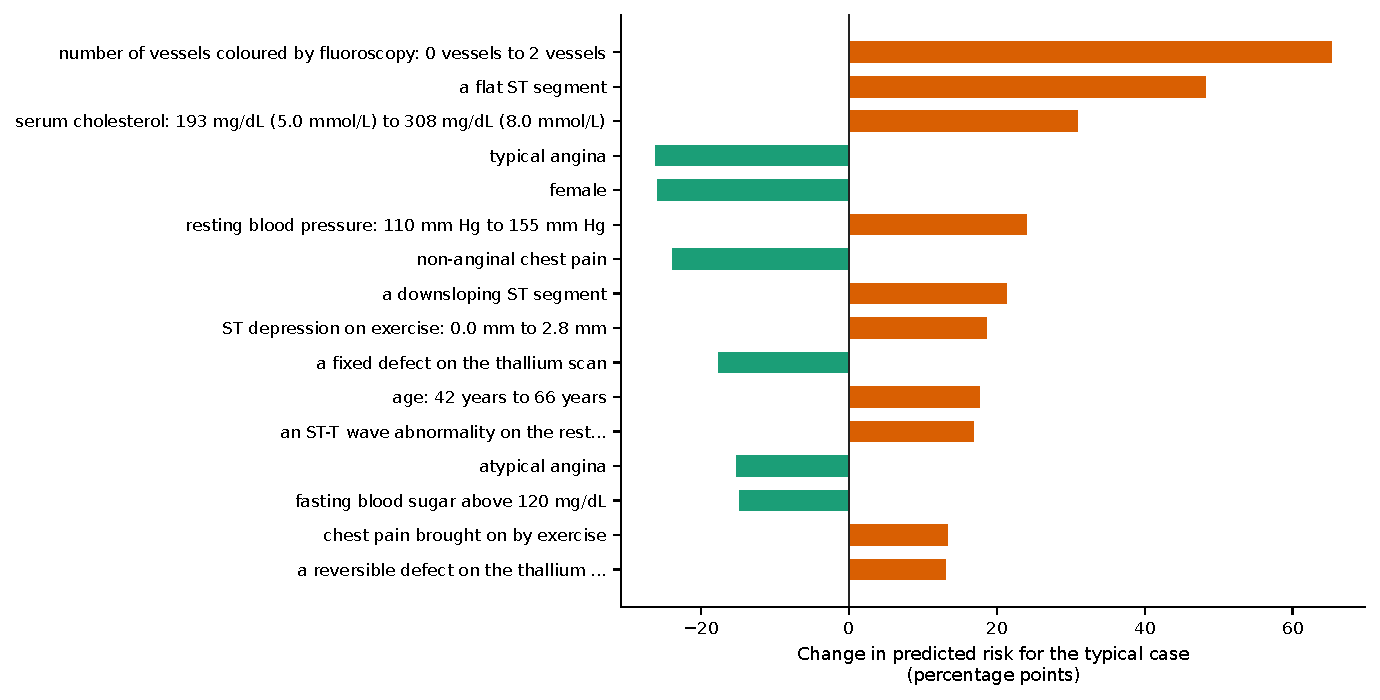
\includegraphics[width=\linewidth,height=0.88\textheight,keepaspectratio]{figures/heart-s2-c1/ann_34-effects.pdf}
\caption{The whole model: Each input's change in the predicted value for the typical case across the whole model, largest first (orange: raises it, teal: lowers it).}
\label{fig:hearts2c1:plot-ann34-0}
\end{figure}
\par\smallskip\noindent{\small \textbf{Dive deeper:} Age and heart rate gate (\ref{rd:ann31}); ST depression hinges (\ref{rd:ann33}); Flat ST segment with cholesterol (\ref{rd:ann32}). Technical detail: \ref{tech:ann34}.\par}
\subsubsection{Age and heart rate gate}\label{rd:ann31}
\noindent{\footnotesize Part of: The whole model (\ref{rd:ann34}).\par}
\noindent{\small Figure~\ref{fig:hearts2c1:parts-ann31} shows what feeds this part; Figure~\ref{fig:hearts2c1:units-ann31} its units and every connection into them (dashed boxes: connections from or to other parts, drawn in their own sections).\par}
\begin{figure}[H]\centering
\resizebox{!}{\ifdim\height>0.5\textheight 0.5\textheight\else\height\fi}{%
\resizebox{\ifdim\width>\linewidth\linewidth\else\width\fi}{!}{%
\begin{tikzpicture}[
  font=\sffamily\scriptsize, >={Stealth[length=1.6mm]},
  inp/.style={draw, rounded corners=1pt, fill=white, inner sep=1.5pt, minimum height=3.2mm, anchor=east},
  abox/.style={draw, thick, rounded corners=2pt, align=center, inner sep=3pt, minimum height=6mm, text width=42mm},
  outp/.style={draw, double, rounded corners=2pt, fill=white, align=center, inner sep=3pt, text width=24mm},
  agg/.style={draw=black!55},
]
\node[inp] (i0) at (0,0.75) {age};
\node[inp] (i1) at (0,-0.0) {maximum heart rate};
\node[inp] (i2) at (0,-0.75) {thallium stress test result};
\node[outp] (out) at (9.36,0) {Age and heart rate gate};
\begin{scope}[on background layer]
\draw[->, agg, thin, dashed] (i0.east) -- (out.west);
\draw[->, agg, thin, dashed] (i1.east) -- (out.west);
\draw[->, agg, thin, dashed] (i2.east) -- (out.west);
\end{scope}
\end{tikzpicture}}}%
\caption{Age and heart rate gate: what feeds it, one level down.}
\label{fig:hearts2c1:parts-ann31}
\end{figure}
\begin{figure}[H]\centering
\resizebox{\ifdim\width>\linewidth\linewidth\else\width\fi}{!}{%
\definecolor{netup}{HTML}{D95F02}\definecolor{netdown}{HTML}{1B9E77}\definecolor{netmixed}{HTML}{7F7F7F}%
\begin{tikzpicture}[
  font=\sffamily\scriptsize, >={Stealth[length=1.4mm]},
  inp/.style={draw, circle, fill=white, minimum size=3.2mm, inner sep=0pt},
  hid/.style={draw, circle, fill=white, minimum size=5.2mm, inner sep=0.5pt, font=\sffamily\tiny},
  exitbox/.style={draw, thick, rectangle, fill=white, align=center, text width=17mm, minimum height=5mm, inner sep=1.5pt, font=\sffamily\tiny},
  sumbox/.style={draw, thick, dashed, rectangle, fill=white, align=center, text width=17mm, minimum height=5mm, inner sep=1.5pt, font=\sffamily\tiny},
  outp/.style={draw, thick, regular polygon, regular polygon sides=6, fill=white, minimum size=10mm, inner sep=0pt, font=\sffamily\tiny, align=center},
  stub/.style={draw, dashed, rounded corners=2pt, fill=white, align=center, inner sep=2pt, font=\sffamily\tiny, text width=15mm},
  inlab/.style={font=\sffamily\tiny, align=center, text width=15mm, inner sep=1pt, fill=white, fill opacity=0.8, text opacity=1},
  wpos/.style={draw=NavyBlue}, wneg/.style={draw=BrickRed}, wagg/.style={draw=black!45, line width=1.2pt},
  wmix/.style={draw=Plum},
]
\node[exitbox] (n1718) at (2.7,3.25) {Age and heart rate gate $\downarrow$};
\node[hid] (n3195) at (2.7,1.9) {h4};
\node[inp, draw=netup, very thick] (ninxxage) at (0.9,0.0) {};
\path (ninxxage.south) node[inlab, anchor=north] (labninxxage) {age $\uparrow$};
\node[inp, draw=netup, very thick] (ninxxthalx7) at (4.5,0.0) {};
\path (ninxxthalx7.south) node[inlab, anchor=north] (labninxxthalx7) {reversible defect $\uparrow$};
\node[inp, draw=netdown, very thick] (ninxxthalach) at (2.7,0.0) {};
\path (ninxxthalach.south) node[inlab, anchor=north] (labninxxthalach) {max heart rate $\downarrow$};
\node[stub] (ntoxxthexmodelxoutput) at (2.7,4.8) {to the model output};
\begin{scope}[on background layer]
\node[fit=(n1718) (n3195) , inner sep=8pt, rounded corners=5pt, fill=BurntOrange!10, draw=BurntOrange!45] (clu0) {};
\draw[->, wneg, line width=0.78pt] (ninxxage) -- (n1718);
\draw[->, wneg, line width=0.51pt] (n3195) -- (n1718);
\draw[->, wneg, line width=0.52pt] (ninxxthalx7) -- (n1718);
\draw[->, wpos, line width=0.63pt] (ninxxthalx7) -- (n3195);
\draw[->, wpos, line width=0.61pt] (ninxxthalach) -- (n1718);
\draw[->, wneg, line width=0.46pt] (n1718) -- (ntoxxthexmodelxoutput);
\end{scope}
\node[font=\sffamily\scriptsize\bfseries, text=BurntOrange!55!black, anchor=south west, inner sep=1pt, fill=white, fill opacity=0.85, text opacity=1] at (clu0.north west) {Age and heart rate gate};
\end{tikzpicture}}%
\caption{Age and heart rate gate: its units and every connection into them. Blue: positive weight (raises the score); red: negative weight (lowers it); thicker: larger weight. Orange outline and up arrow: raises the final prediction; teal and down arrow: lowers it; grey and double arrow: depends.}
\label{fig:hearts2c1:units-ann31}
\end{figure}
\paragraph{Hypothesis.} This part lowers the predicted risk for patients whose age is low relative to their maximum heart rate; for the typical patient it acts on, a reversible defect on the thallium scan raises the risk through it from about 1\% to about 4\%.\,{\scriptsize\textcolor{NavyBlue}{[C54, C32]}}
\paragraph{Evidence.} For patients without a reversible defect on the thallium scan, it switches on when age in years minus about 0.28 $\times$ the maximum heart rate in beats per minute is below about 11.4 (for maximum heart rates from about 71 to 202 beats per minute); 80 of 242 training patients are on that side, and 11\% of them had heart disease, against 60\% of the others.\,{\scriptsize\textcolor{NavyBlue}{[C54]}} Through it, older age raises the predicted risk steadily up to about 56 years (between 45 and 61 years for different patients), then no further for most patients, but for patients with a reversible defect on the thallium scan it rises in a jump: for a typical patient from about 12\% at 42 to about 29\% at 66 years.\,{\scriptsize\textcolor{NavyBlue}{[C30, C37]}} Across the whole model, older age raises the risk, then no further, only if the thallium scan shows no reversible defect: from about 12\% to about 29\%, while with one it stays at about 42\%.\,{\scriptsize\textcolor{NavyBlue}{[C33]}} A higher maximum heart rate lowers the risk through it in an uneven way, from about 29\% at 118 to about 22\% at 175 beats per minute, and across the whole model it lowers it more without a reversible defect (from about 32\% to about 21\%, against about 45\% to about 40\%).\,{\scriptsize\textcolor{NavyBlue}{[C31, C35]}} Its formula reproduces the part exactly on all 242 training patients.\,{\scriptsize\textcolor{NavyBlue}{[C39]}}
\par\noindent{\small Evidence plots: Figure~\ref{fig:hearts2c1:plot-ann31-0}, Figure~\ref{fig:hearts2c1:plot-ann31-1}, Figure~\ref{fig:hearts2c1:plot-ann31-2}, Figure~\ref{fig:hearts2c1:plot-ann31-3}, Figure~\ref{fig:hearts2c1:plot-ann31-4}, Figure~\ref{fig:hearts2c1:plot-ann31-5}, Figure~\ref{fig:hearts2c1:plot-ann31-6}, Figure~\ref{fig:hearts2c1:plot-ann31-7}.\par}
\par\medskip\noindent\textbf{Worked example: reading this part.} Figure~\ref{fig:hearts2c1:plot-ann31-3} maps the part's own output over its main inputs. In the grey region it is switched off and adds nothing; past the black line it switches on, and the colour shows how much it adds to the score. The line is the rule in the claim (C54): it switches on when age minus about 0.28 $\times$ maximum heart rate below about 11.4 (for maximum heart rate from about 71.0 to 202). 80 of 242 training patients lie on the 'on' side, and 11\% of them had heart disease, against 60\% of the others: the 'on' side holds mostly hollow points, so the part picks out low-risk cases. Figure~\ref{fig:hearts2c1:plot-ann31-4} cuts the map into slices: the hinge moves as the other input changes, which is what a tilted line means. Figure~\ref{fig:hearts2c1:plot-ann31-5} shows what this does to the final prediction for the typical case.\par
\par\noindent{\small Figure~\ref{fig:hearts2c1:plot-ann31-6} shows this part's own output, unit h2: over its two main inputs, with the line where it switches on.\par}
\begin{figure}[H]\centering
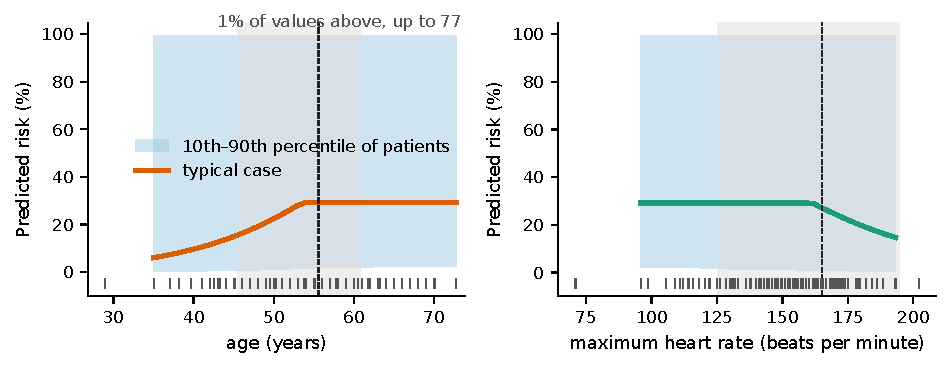
\includegraphics[width=\linewidth,height=0.88\textheight,keepaspectratio]{figures/heart-s2-c1/ann_31-response.pdf}
\caption{Age and heart rate gate: Response curves through this part: the typical case (bold), the 10th to 90th percentile of individual patients (band), the fold or step point (dashed) with its spread across them (grey), and the observed values (ticks).}
\label{fig:hearts2c1:plot-ann31-0}
\end{figure}
\begin{figure}[H]\centering
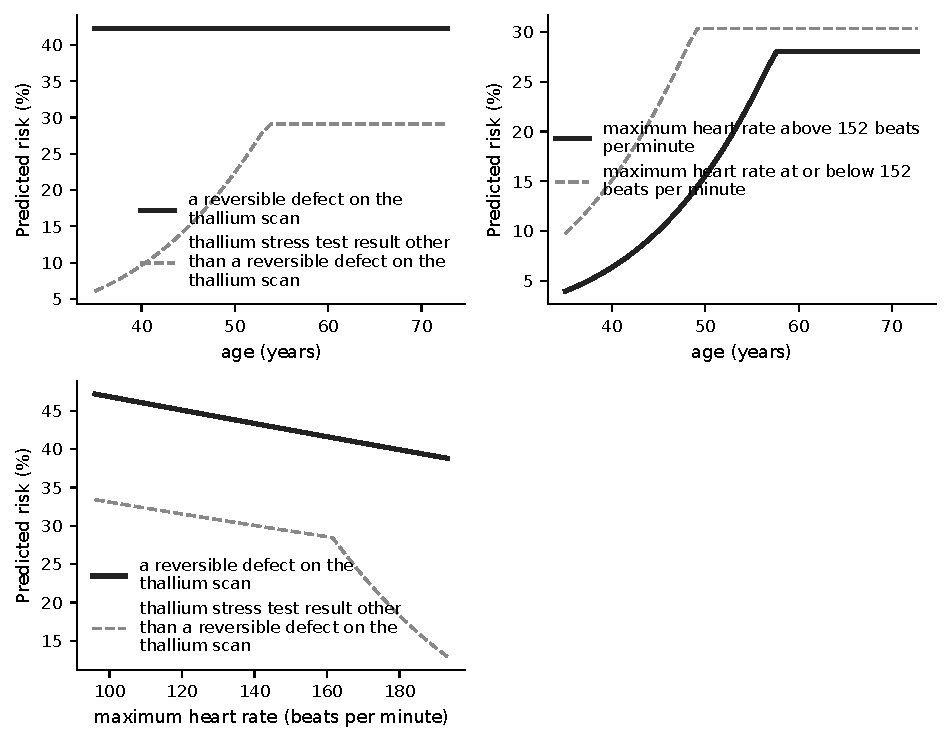
\includegraphics[width=\linewidth,height=0.88\textheight,keepaspectratio]{figures/heart-s2-c1/ann_31-interaction.pdf}
\caption{Age and heart rate gate: How the effect differs between groups: one curve per group, for the typical case of each group.}
\label{fig:hearts2c1:plot-ann31-1}
\end{figure}
\begin{figure}[H]\centering
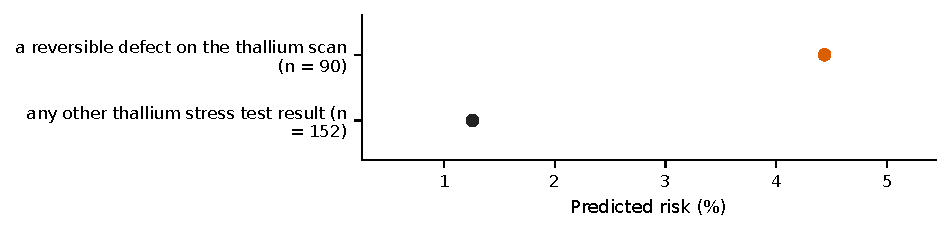
\includegraphics[width=\linewidth,height=0.88\textheight,keepaspectratio]{figures/heart-s2-c1/ann_31-categories-small.pdf}
\caption{Age and heart rate gate: The predicted value for the typical case at each level, through this part (n = training patients; grey: fewer than 20).}
\label{fig:hearts2c1:plot-ann31-2}
\end{figure}
\begin{figure}[H]\centering
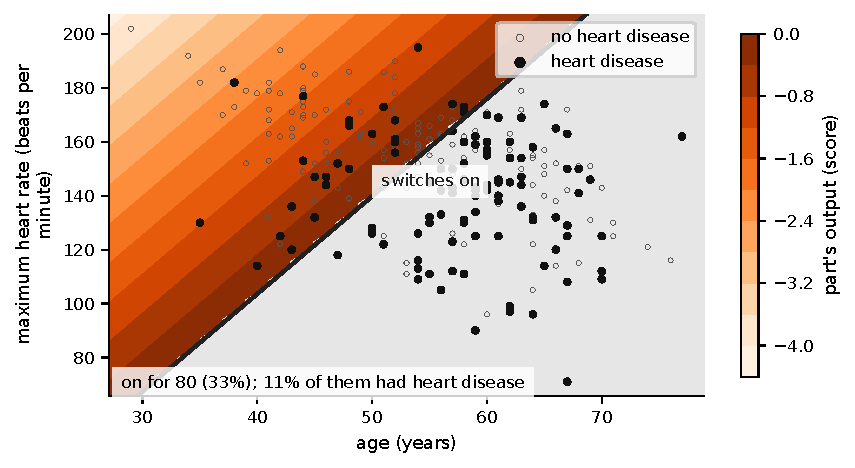
\includegraphics[width=\linewidth,height=0.88\textheight,keepaspectratio]{figures/heart-s2-c1/ann_31-deep-map.pdf}
\caption{Age and heart rate gate: The part's own output over its two numeric inputs, other inputs at the typical case: colour where it is on, flat grey where it is switched off, the black line where it switches on; training patients as hollow (no event) and filled (event) points, so the part can be seen catching the events (the predicted-chance overlay was harder to read).}
\label{fig:hearts2c1:plot-ann31-3}
\end{figure}
\begin{figure}[H]\centering
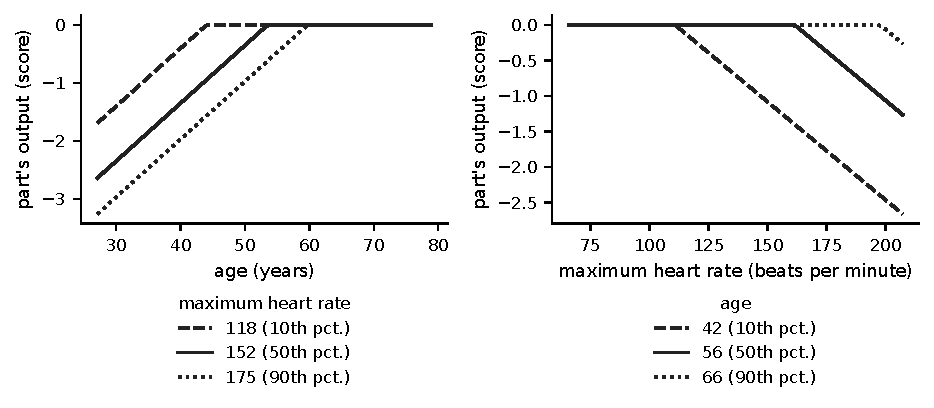
\includegraphics[width=\linewidth,height=0.88\textheight,keepaspectratio]{figures/heart-s2-c1/ann_31-deep-slices.pdf}
\caption{Age and heart rate gate: Slices of the same map: the part's own output against each input at three values of the other, so the tilted boundary shows as a shifting hinge.}
\label{fig:hearts2c1:plot-ann31-4}
\end{figure}
\begin{figure}[H]\centering
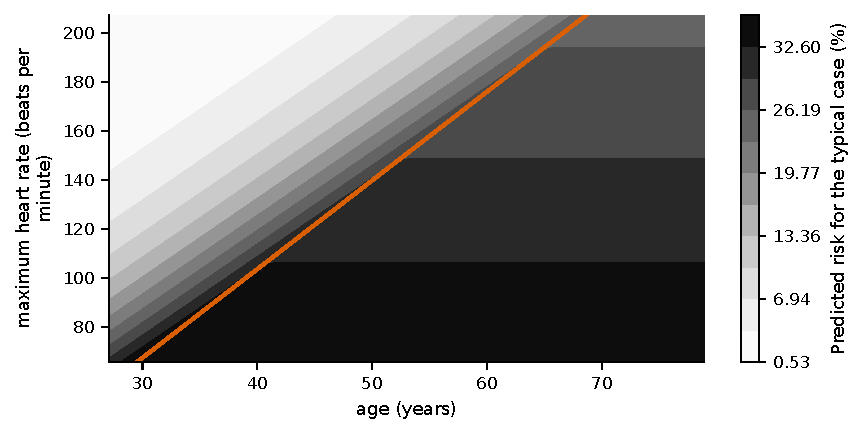
\includegraphics[width=\linewidth,height=0.88\textheight,keepaspectratio]{figures/heart-s2-c1/ann_31-deep-risk.pdf}
\caption{Age and heart rate gate: The same map on the final scale: the predicted value for the typical case, with the switch-on line (orange).}
\label{fig:hearts2c1:plot-ann31-5}
\end{figure}
\begin{figure}[H]\centering
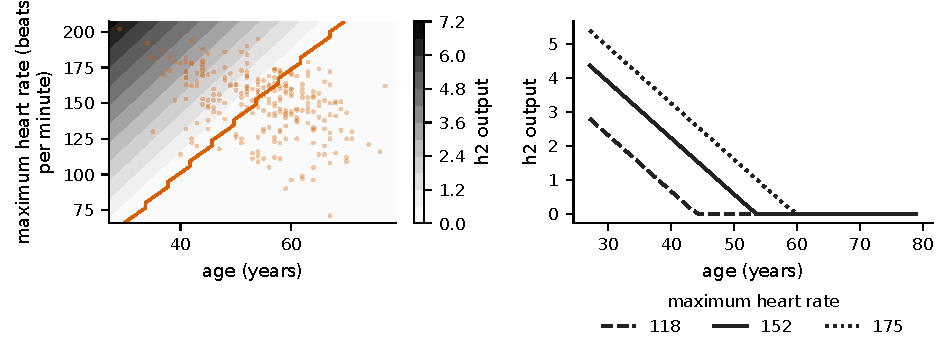
\includegraphics[width=\linewidth,height=0.88\textheight,keepaspectratio]{figures/heart-s2-c1/ann_31-partial-1718.pdf}
\caption{Age and heart rate gate: This part's own output, unit h2 (the output of 'Age and heart rate gate'), on its own scale (its activation), with every other input at the typical case; it is active for 80 of 242. Left: its output over its two main inputs (orange line: where it switches on; dots: the data); right: slices at three values of the second input.}
\label{fig:hearts2c1:plot-ann31-6}
\end{figure}
\begin{figure}[H]\centering
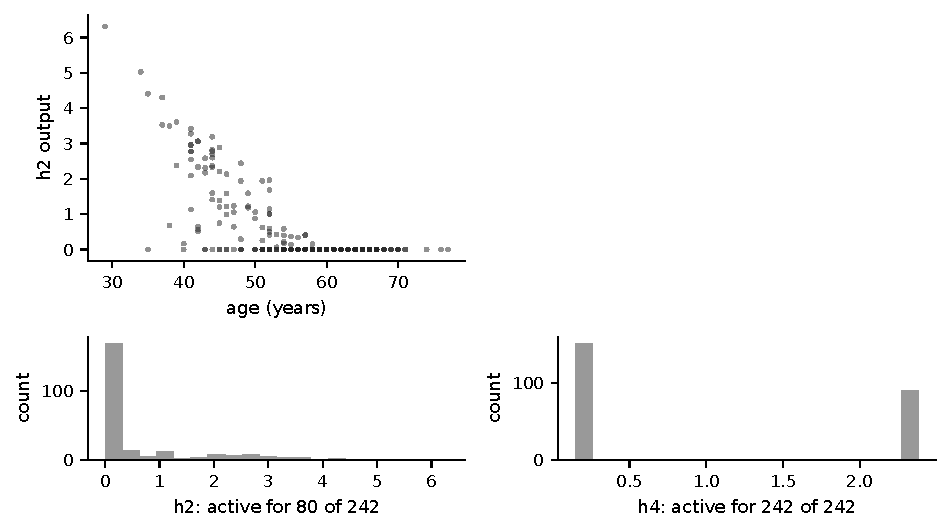
\includegraphics[width=\linewidth,height=0.88\textheight,keepaspectratio]{figures/heart-s2-c1/ann_31-units.pdf}
\caption{Age and heart rate gate: This part's hidden units: each unit's output against its main numeric input (top) and how often it is active (bottom).}
\label{fig:hearts2c1:plot-ann31-7}
\end{figure}
\par\smallskip\noindent{\small Technical detail: \ref{tech:ann31}.\par}
\subsubsection{ST depression hinges}\label{rd:ann33}
\noindent{\footnotesize Part of: The whole model (\ref{rd:ann34}).\par}
\noindent{\small Figure~\ref{fig:hearts2c1:parts-ann33} shows what feeds this part; Figure~\ref{fig:hearts2c1:units-ann33} its units and every connection into them (dashed boxes: connections from or to other parts, drawn in their own sections).\par}
\begin{figure}[H]\centering
\resizebox{!}{\ifdim\height>0.5\textheight 0.5\textheight\else\height\fi}{%
\resizebox{\ifdim\width>\linewidth\linewidth\else\width\fi}{!}{%
\begin{tikzpicture}[
  font=\sffamily\scriptsize, >={Stealth[length=1.6mm]},
  inp/.style={draw, rounded corners=1pt, fill=white, inner sep=1.5pt, minimum height=3.2mm, anchor=east},
  abox/.style={draw, thick, rounded corners=2pt, align=center, inner sep=3pt, minimum height=6mm, text width=42mm},
  outp/.style={draw, double, rounded corners=2pt, fill=white, align=center, inner sep=3pt, text width=24mm},
  agg/.style={draw=black!55},
]
\node[inp] (i0) at (0,-0.0) {ST depression on exercise};
\node[outp] (out) at (9.36,0) {ST depression hinges};
\begin{scope}[on background layer]
\draw[->, agg, thin, dashed] (i0.east) -- (out.west);
\end{scope}
\end{tikzpicture}}}%
\caption{ST depression hinges: what feeds it, one level down.}
\label{fig:hearts2c1:parts-ann33}
\end{figure}
\begin{figure}[H]\centering
\resizebox{\ifdim\width>\linewidth\linewidth\else\width\fi}{!}{%
\definecolor{netup}{HTML}{D95F02}\definecolor{netdown}{HTML}{1B9E77}\definecolor{netmixed}{HTML}{7F7F7F}%
\begin{tikzpicture}[
  font=\sffamily\scriptsize, >={Stealth[length=1.4mm]},
  inp/.style={draw, circle, fill=white, minimum size=3.2mm, inner sep=0pt},
  hid/.style={draw, circle, fill=white, minimum size=5.2mm, inner sep=0.5pt, font=\sffamily\tiny},
  exitbox/.style={draw, thick, rectangle, fill=white, align=center, text width=17mm, minimum height=5mm, inner sep=1.5pt, font=\sffamily\tiny},
  sumbox/.style={draw, thick, dashed, rectangle, fill=white, align=center, text width=17mm, minimum height=5mm, inner sep=1.5pt, font=\sffamily\tiny},
  outp/.style={draw, thick, regular polygon, regular polygon sides=6, fill=white, minimum size=10mm, inner sep=0pt, font=\sffamily\tiny, align=center},
  stub/.style={draw, dashed, rounded corners=2pt, fill=white, align=center, inner sep=2pt, font=\sffamily\tiny, text width=15mm},
  inlab/.style={font=\sffamily\tiny, align=center, text width=15mm, inner sep=1pt, fill=white, fill opacity=0.8, text opacity=1},
  wpos/.style={draw=NavyBlue}, wneg/.style={draw=BrickRed}, wagg/.style={draw=black!45, line width=1.2pt},
  wmix/.style={draw=Plum},
]
\node[hid] (n1946) at (2.0,1.9) {h3};
\node[hid] (n3284) at (2.0,3.25) {h5};
\node[inp, draw=netup, very thick] (ninxxoldpeak) at (2.0,0.0) {};
\path (ninxxoldpeak.south) node[inlab, anchor=north] (labninxxoldpeak) {ST depression $\uparrow$};
\node[stub] (ntoxxthexmodelxoutput) at (2.0,4.8) {to the model output};
\begin{scope}[on background layer]
\node[fit=(n1946) (n3284) , inner sep=8pt, rounded corners=5pt, fill=ForestGreen!10, draw=ForestGreen!45] (clu0) {};
\draw[->, wpos, line width=0.60pt] (n1946) -- (n3284);
\draw[->, wpos, line width=0.51pt] (ninxxoldpeak) -- (n1946);
\draw[->, wpos, line width=0.38pt] (n1946) -- (ntoxxthexmodelxoutput);
\draw[->, wpos, line width=0.40pt] (n3284) -- (ntoxxthexmodelxoutput);
\end{scope}
\node[font=\sffamily\scriptsize\bfseries, text=ForestGreen!55!black, anchor=south west, inner sep=1pt, fill=white, fill opacity=0.85, text opacity=1] at (clu0.north west) {ST depression hinges};
\end{tikzpicture}}%
\caption{ST depression hinges: its units and every connection into them. Blue: positive weight (raises the score); red: negative weight (lowers it); thicker: larger weight. Orange outline and up arrow: raises the final prediction; teal and down arrow: lowers it; grey and double arrow: depends.}
\label{fig:hearts2c1:units-ann33}
\end{figure}
\paragraph{Hypothesis.} This part raises the predicted risk with ST depression on exercise, slowly at first, then faster, adding risk only once it rises above about 0.8 mm.\,{\scriptsize\textcolor{NavyBlue}{[C40, C41]}}
\paragraph{Evidence.} It acts on 121 of 242 training patients, 77 of whom had heart disease; for the typical patient it acts on, the predicted risk is about 89\% without it and about 91\% with it.\,{\scriptsize\textcolor{NavyBlue}{[C42]}} Through it, more ST depression raises the risk slowly at first, then faster, adding risk only once it rises above about 0.8 mm: for a typical patient from about 29\% at 0 mm to about 48\% at 2.8 mm.\,{\scriptsize\textcolor{NavyBlue}{[C40, C41]}} Its formula reproduces the part exactly on all 242 training patients.\,{\scriptsize\textcolor{NavyBlue}{[C43]}}
\par\noindent{\small Evidence plots: Figure~\ref{fig:hearts2c1:plot-ann33-0}, Figure~\ref{fig:hearts2c1:plot-ann33-1}, Figure~\ref{fig:hearts2c1:plot-ann33-2}, Figure~\ref{fig:hearts2c1:plot-ann33-3}.\par}
\par\noindent{\small Figure~\ref{fig:hearts2c1:plot-ann33-1} shows this part's own output, unit h3: it switches on at about 0.7582 mm of ST depression on exercise, and is zero below.\par}
\par\noindent{\small Figure~\ref{fig:hearts2c1:plot-ann33-2} shows this part's own output, unit h5: it switches on at about 1.666 mm of ST depression on exercise, and is zero below.\par}
\begin{figure}[H]\centering
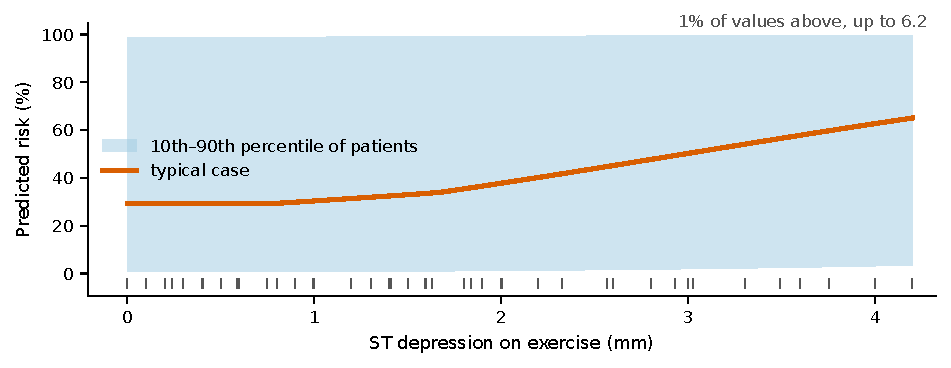
\includegraphics[width=\linewidth,height=0.88\textheight,keepaspectratio]{figures/heart-s2-c1/ann_33-response.pdf}
\caption{ST depression hinges: Response curves through this part: the typical case (bold), the 10th to 90th percentile of individual patients (band), the fold or step point (dashed) with its spread across them (grey), and the observed values (ticks).}
\label{fig:hearts2c1:plot-ann33-0}
\end{figure}
\begin{figure}[H]\centering
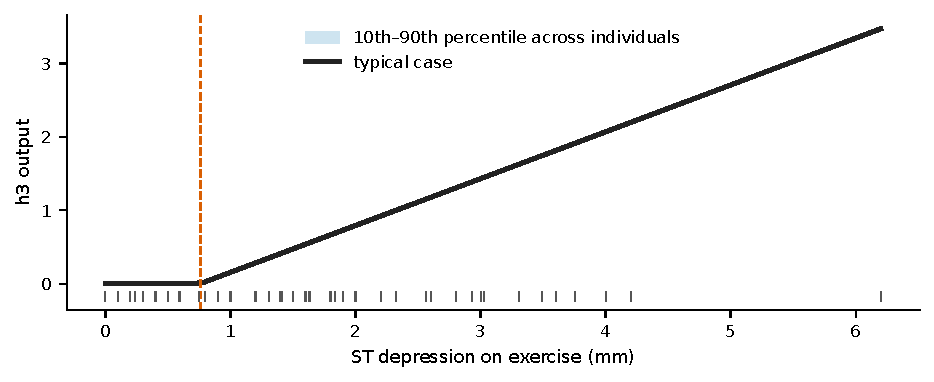
\includegraphics[width=\linewidth,height=0.88\textheight,keepaspectratio]{figures/heart-s2-c1/ann_33-partial-1946.pdf}
\caption{ST depression hinges: This part's own output, unit h3 (the output of 'ST depression hinges'), on its own scale (its activation), with every other input at the typical case; it is active for 121 of 242. Bold: the typical case; band: 10th to 90th percentile across individuals; dashed: where it switches on; ticks: the data.}
\label{fig:hearts2c1:plot-ann33-1}
\end{figure}
\begin{figure}[H]\centering
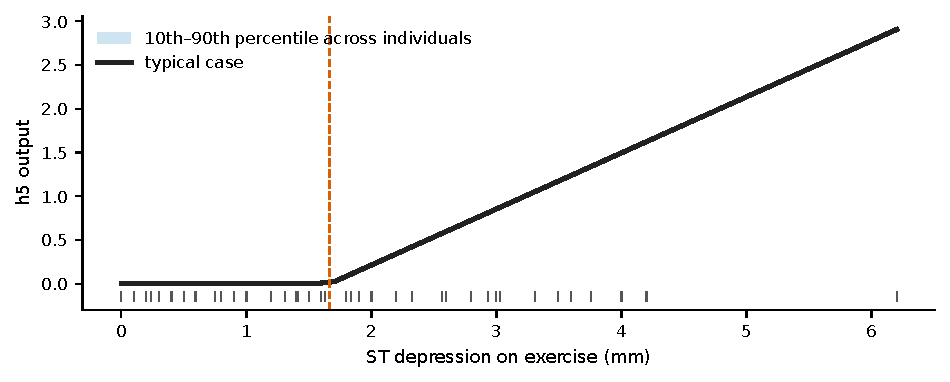
\includegraphics[width=\linewidth,height=0.88\textheight,keepaspectratio]{figures/heart-s2-c1/ann_33-partial-3284.pdf}
\caption{ST depression hinges: This part's own output, unit h5 (the output of 'ST depression hinges'), on its own scale (its activation), with every other input at the typical case; it is active for 58 of 242. Bold: the typical case; band: 10th to 90th percentile across individuals; dashed: where it switches on; ticks: the data.}
\label{fig:hearts2c1:plot-ann33-2}
\end{figure}
\begin{figure}[H]\centering
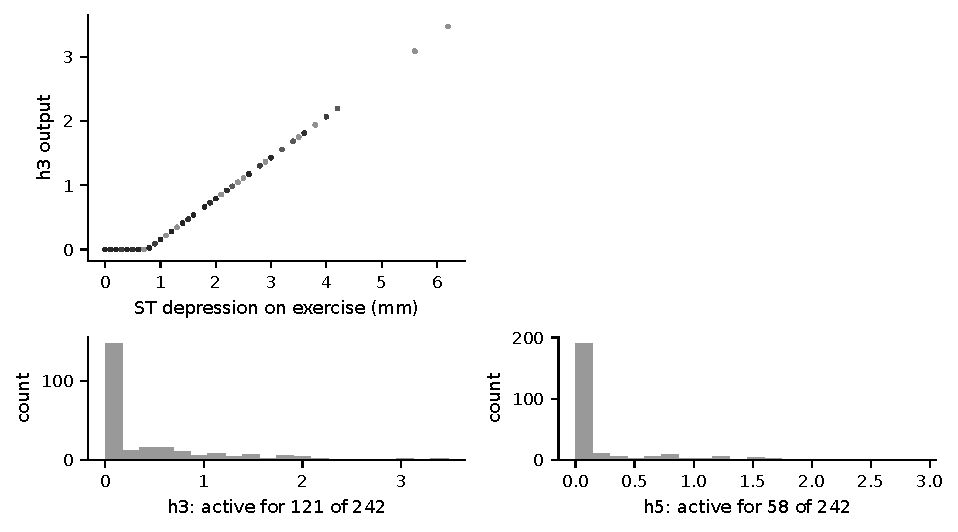
\includegraphics[width=\linewidth,height=0.88\textheight,keepaspectratio]{figures/heart-s2-c1/ann_33-units.pdf}
\caption{ST depression hinges: This part's hidden units: each unit's output against its main numeric input (top) and how often it is active (bottom).}
\label{fig:hearts2c1:plot-ann33-3}
\end{figure}
\par\smallskip\noindent{\small Technical detail: \ref{tech:ann33}.\par}
\subsubsection{Flat ST segment with cholesterol}\label{rd:ann32}
\noindent{\footnotesize Part of: The whole model (\ref{rd:ann34}).\par}
\noindent{\small Figure~\ref{fig:hearts2c1:parts-ann32} shows what feeds this part; Figure~\ref{fig:hearts2c1:units-ann32} its units and every connection into them (dashed boxes: connections from or to other parts, drawn in their own sections).\par}
\begin{figure}[H]\centering
\resizebox{!}{\ifdim\height>0.5\textheight 0.5\textheight\else\height\fi}{%
\resizebox{\ifdim\width>\linewidth\linewidth\else\width\fi}{!}{%
\begin{tikzpicture}[
  font=\sffamily\scriptsize, >={Stealth[length=1.6mm]},
  inp/.style={draw, rounded corners=1pt, fill=white, inner sep=1.5pt, minimum height=3.2mm, anchor=east},
  abox/.style={draw, thick, rounded corners=2pt, align=center, inner sep=3pt, minimum height=6mm, text width=42mm},
  outp/.style={draw, double, rounded corners=2pt, fill=white, align=center, inner sep=3pt, text width=24mm},
  agg/.style={draw=black!55},
]
\node[inp] (i0) at (0,0.75) {serum cholesterol};
\node[inp] (i1) at (0,-0.0) {ST depression on exercise};
\node[inp] (i2) at (0,-0.75) {slope of the ST segment at peak exercise};
\node[outp] (out) at (9.36,0) {Flat ST segment with cholesterol};
\begin{scope}[on background layer]
\draw[->, agg, thin, dashed] (i0.east) -- (out.west);
\draw[->, agg, thin, dashed] (i1.east) -- (out.west);
\draw[->, agg, thin, dashed] (i2.east) -- (out.west);
\end{scope}
\end{tikzpicture}}}%
\caption{Flat ST segment with cholesterol: what feeds it, one level down.}
\label{fig:hearts2c1:parts-ann32}
\end{figure}
\begin{figure}[H]\centering
\resizebox{\ifdim\width>\linewidth\linewidth\else\width\fi}{!}{%
\definecolor{netup}{HTML}{D95F02}\definecolor{netdown}{HTML}{1B9E77}\definecolor{netmixed}{HTML}{7F7F7F}%
\begin{tikzpicture}[
  font=\sffamily\scriptsize, >={Stealth[length=1.4mm]},
  inp/.style={draw, circle, fill=white, minimum size=3.2mm, inner sep=0pt},
  hid/.style={draw, circle, fill=white, minimum size=5.2mm, inner sep=0.5pt, font=\sffamily\tiny},
  exitbox/.style={draw, thick, rectangle, fill=white, align=center, text width=17mm, minimum height=5mm, inner sep=1.5pt, font=\sffamily\tiny},
  sumbox/.style={draw, thick, dashed, rectangle, fill=white, align=center, text width=17mm, minimum height=5mm, inner sep=1.5pt, font=\sffamily\tiny},
  outp/.style={draw, thick, regular polygon, regular polygon sides=6, fill=white, minimum size=10mm, inner sep=0pt, font=\sffamily\tiny, align=center},
  stub/.style={draw, dashed, rounded corners=2pt, fill=white, align=center, inner sep=2pt, font=\sffamily\tiny, text width=15mm},
  inlab/.style={font=\sffamily\tiny, align=center, text width=15mm, inner sep=1pt, fill=white, fill opacity=0.8, text opacity=1},
  wpos/.style={draw=NavyBlue}, wneg/.style={draw=BrickRed}, wagg/.style={draw=black!45, line width=1.2pt},
  wmix/.style={draw=Plum},
]
\node[hid] (n3464) at (3.2,1.9) {h6};
\node[exitbox] (n1476) at (3.2,3.25) {Flat ST segment with cholesterol $\uparrow$};
\node[inp, draw=netdown, very thick] (ninxxchol) at (3.2,0.0) {};
\path (ninxxchol.south) node[inlab, anchor=north] (labninxxchol) {cholesterol $\downarrow$};
\node[inp, draw=netup, very thick] (ninxxslopex2) at (5.0,0.0) {};
\path (ninxxslopex2.south) node[inlab, anchor=north] (labninxxslopex2) {flat ST $\uparrow$};
\node[inp, draw=netup, very thick] (ninxxoldpeak) at (1.4,0.0) {};
\path (ninxxoldpeak.south) node[inlab, anchor=north] (labninxxoldpeak) {ST depression $\uparrow$};
\node[stub] (ntoxxthexmodelxoutput) at (3.2,4.8) {to the model output};
\begin{scope}[on background layer]
\node[fit=(n3464) (n1476) , inner sep=8pt, rounded corners=5pt, fill=Orchid!10, draw=Orchid!45] (clu0) {};
\draw[->, wneg, line width=0.38pt] (n3464) -- (n1476);
\draw[->, wpos, line width=0.60pt] (ninxxchol) -- (n3464);
\draw[->, wpos, line width=0.65pt] (ninxxslopex2) -- (n1476);
\draw[->, wpos, line width=0.52pt] (ninxxoldpeak) -- (n1476);
\draw[->, wpos, line width=0.34pt] (n1476) -- (ntoxxthexmodelxoutput);
\end{scope}
\node[font=\sffamily\scriptsize\bfseries, text=Orchid!55!black, anchor=south west, inner sep=1pt, fill=white, fill opacity=0.85, text opacity=1] at (clu0.north west) {Flat ST segment with cholesterol};
\end{tikzpicture}}%
\caption{Flat ST segment with cholesterol: its units and every connection into them. Blue: positive weight (raises the score); red: negative weight (lowers it); thicker: larger weight. Orange outline and up arrow: raises the final prediction; teal and down arrow: lowers it; grey and double arrow: depends.}
\label{fig:hearts2c1:units-ann32}
\end{figure}
\paragraph{Hypothesis.} This part raises the predicted risk mainly for patients with a flat ST segment, and makes ST depression on exercise count more for them, rising slowly at first, then faster.\,{\scriptsize\textcolor{NavyBlue}{[C44, C48]}}
\paragraph{Evidence.} It acts on 117 of 242 training patients, 78 of whom had heart disease; for the typical patient it acts on, the predicted risk is about 86\% without it and about 90\% with it.\,{\scriptsize\textcolor{NavyBlue}{[C52]}} For patients whose ST segment is not flat, it switches on when ST depression on exercise is above about 2.23 mm (for cholesterol from about 126 to 186 mg/dL), or when ST depression minus about 0.012 $\times$ the cholesterol in mg/dL is above about 0.011 (for cholesterol from about 186 to 417 mg/dL); 117 of 242 training patients are on, and 67\% of them had heart disease, against 23\% of the others.\,{\scriptsize\textcolor{NavyBlue}{[C55]}} Through it, a flat ST segment raises a typical patient's predicted risk from about 29\% to about 34\%; for the typical patient it acts on, more ST depression raises it in an uneven way from about 87\% to about 92\%, and higher cholesterol lowers it in an uneven way from about 91\% to about 88\%.\,{\scriptsize\textcolor{NavyBlue}{[C44, C45, C46]}} Across the whole model, more ST depression raises the risk slowly at first, then faster, from about 75\% to about 91\% with a flat ST segment, against about 29\% to about 48\% otherwise.\,{\scriptsize\textcolor{NavyBlue}{[C48]}} Its formula reproduces the part exactly on all 242 training patients.\,{\scriptsize\textcolor{NavyBlue}{[C53]}}
\par\noindent{\small Evidence plots: Figure~\ref{fig:hearts2c1:plot-ann32-0}, Figure~\ref{fig:hearts2c1:plot-ann32-1}, Figure~\ref{fig:hearts2c1:plot-ann32-2}, Figure~\ref{fig:hearts2c1:plot-ann32-3}, Figure~\ref{fig:hearts2c1:plot-ann32-4}, Figure~\ref{fig:hearts2c1:plot-ann32-5}, Figure~\ref{fig:hearts2c1:plot-ann32-6}, Figure~\ref{fig:hearts2c1:plot-ann32-7}.\par}
\par\medskip\noindent\textbf{Worked example: reading this part.} Figure~\ref{fig:hearts2c1:plot-ann32-3} maps the part's own output over its main inputs. In the grey region it is switched off and adds nothing; past the black line it switches on, and the colour shows how much it adds to the score. The line is the rule in the claim (C55): it switches on when ST depression on exercise above about 2.23 (for serum cholesterol from about 126 to 186); ST depression on exercise minus about 0.012 $\times$ serum cholesterol above about 0.011 (for serum cholesterol from about 186 to 417). 117 of 242 training patients lie on the 'on' side, and 67\% of them had heart disease, against 23\% of the others: the filled points crowd on the 'on' side. Figure~\ref{fig:hearts2c1:plot-ann32-4} cuts the map into slices: the hinge moves as the other input changes, which is what a tilted line means. Figure~\ref{fig:hearts2c1:plot-ann32-5} shows what this does to the final prediction for the typical case.\par
\par\noindent{\small Figure~\ref{fig:hearts2c1:plot-ann32-6} shows this part's own output, unit h1: it switches on at about 2.935 mm of ST depression on exercise, and is zero below.\par}
\begin{figure}[H]\centering
\includegraphics[width=\linewidth,height=0.88\textheight,keepaspectratio]{figures/heart-s2-c1/ann_32-response.pdf}
\caption{Flat ST segment with cholesterol: Response curves through this part: the typical case (bold), the 10th to 90th percentile of individual patients (band), the fold or step point (dashed) with its spread across them (grey), and the observed values (ticks).}
\label{fig:hearts2c1:plot-ann32-0}
\end{figure}
\begin{figure}[H]\centering
\includegraphics[width=\linewidth,height=0.88\textheight,keepaspectratio]{figures/heart-s2-c1/ann_32-interaction.pdf}
\caption{Flat ST segment with cholesterol: How the effect differs between groups: one curve per group, for the typical case of each group.}
\label{fig:hearts2c1:plot-ann32-1}
\end{figure}
\begin{figure}[H]\centering
\includegraphics[width=\linewidth,height=0.88\textheight,keepaspectratio]{figures/heart-s2-c1/ann_32-categories-small.pdf}
\caption{Flat ST segment with cholesterol: The predicted value for the typical case at each level, through this part (n = training patients; grey: fewer than 20).}
\label{fig:hearts2c1:plot-ann32-2}
\end{figure}
\begin{figure}[H]\centering
\includegraphics[width=\linewidth,height=0.88\textheight,keepaspectratio]{figures/heart-s2-c1/ann_32-deep-map.pdf}
\caption{Flat ST segment with cholesterol: The part's own output over its two numeric inputs, other inputs at the typical case: colour where it is on, flat grey where it is switched off, the black line where it switches on; training patients as hollow (no event) and filled (event) points, so the part can be seen catching the events (the predicted-chance overlay was harder to read).}
\label{fig:hearts2c1:plot-ann32-3}
\end{figure}
\begin{figure}[H]\centering
\includegraphics[width=\linewidth,height=0.88\textheight,keepaspectratio]{figures/heart-s2-c1/ann_32-deep-slices.pdf}
\caption{Flat ST segment with cholesterol: Slices of the same map: the part's own output against each input at three values of the other, so the tilted boundary shows as a shifting hinge.}
\label{fig:hearts2c1:plot-ann32-4}
\end{figure}
\begin{figure}[H]\centering
\includegraphics[width=\linewidth,height=0.88\textheight,keepaspectratio]{figures/heart-s2-c1/ann_32-deep-risk.pdf}
\caption{Flat ST segment with cholesterol: The same map on the final scale: the predicted value for the typical case, with the switch-on line (orange).}
\label{fig:hearts2c1:plot-ann32-5}
\end{figure}
\begin{figure}[H]\centering
\includegraphics[width=\linewidth,height=0.88\textheight,keepaspectratio]{figures/heart-s2-c1/ann_32-partial-1476.pdf}
\caption{Flat ST segment with cholesterol: This part's own output, unit h1 (the output of 'Flat ST segment with cholesterol'), on its own scale (its activation), with every other input at the typical case; it is active for 117 of 242. Bold: the typical case; band: 10th to 90th percentile across individuals; dashed: where it switches on; ticks: the data.}
\label{fig:hearts2c1:plot-ann32-6}
\end{figure}
\begin{figure}[H]\centering
\includegraphics[width=\linewidth,height=0.88\textheight,keepaspectratio]{figures/heart-s2-c1/ann_32-units.pdf}
\caption{Flat ST segment with cholesterol: This part's hidden units: each unit's output against its main numeric input (top) and how often it is active (bottom).}
\label{fig:hearts2c1:plot-ann32-7}
\end{figure}
\par\smallskip\noindent{\small Technical detail: \ref{tech:ann32}.\par}
\subsection{Not supported by the model}
\begin{itemize}\setlength\itemsep{0pt}\small
\item C49: interaction claim about serum cholesterol and ST depression during exercise (compared with rest) in part ann\_\allowbreak{}32: not supported by the model (the group difference is below 0.1 log-odds).
\end{itemize}
\clearpage\section*{Technical detail: heart-s2-c1}
\addcontentsline{toc}{section}{Technical detail: heart-s2-c1}
\noindent{\small The record behind each part: the original hypothesis, the closed form, and every claim with its estimate (log-odds and odds ratio), range across patients, n and test check.\par}
\renewcommand{\thesubsection}{T.\arabic{subsection}}\setcounter{subsection}{0}
\subsection{The whole model}\label{tech:ann34}
\noindent{\footnotesize Annotation ann\_\allowbreak{}34 (heart\_\allowbreak{}disease\_\allowbreak{}logit). Reads: age, sex, chest pain type, resting blood pressure, serum cholesterol, fasting blood sugar, resting ECG, maximum heart rate reached during the exercise test, exercise-induced angina, ST depression during exercise (compared with rest), slope of the ST segment at peak exercise, number of major vessels coloured by fluoroscopy, thallium stress test result.\par}
\paragraph{Original hypothesis (unchanged).} Root: p = sigmoid(z), z = -0.227 + LINEAR CORE - 0.605*\allowbreak{}age\_\allowbreak{}hr\_\allowbreak{}reserve\_\allowbreak{}gate + 0.248*\allowbreak{}st\_\allowbreak{}slope\_\allowbreak{}chol\_\allowbreak{}gate + 0.378*\allowbreak{}oldpeak\_\allowbreak{}hinges[1946]\allowbreak{} + 0.419*\allowbreak{}oldpeak\_\allowbreak{}hinges[3284]\allowbreak{}. LINEAR CORE (16 direct input-$>$output edges, z-scored inputs): ca +1.653, cp:4 +0.986, sex:0 -0.742, chol +0.613, slope:2 +0.495, trestbps +0.465, slope:1 -0.453, sex:1 +0.447, cp:2 +0.397, fbs:1 -0.308, thal:7 +0.279, exang:1 +0.278, thal:6 -0.278, cp:1 -0.180, thalach -0.079, restecg:1 +0.066. Eight inputs are unused (cp:3, fbs:0, restecg:0, restecg:2, exang:0, slope:3, thal:3, thal:4; zero-effect entries of this root). Age and oldpeak have no direct edge; they act only through the children. COMPOSITION: purely additive in the logit. The three children add nonlinear corrections to the linear core: (1) age\_\allowbreak{}hr\_\allowbreak{}reserve\_\allowbreak{}gate, a protective ReLU on when max heart rate is high for age and there is no reversible thallium defect; (2) st\_\allowbreak{}slope\_\allowbreak{}chol\_\allowbreak{}gate, a flat-ST-slope indicator scaled up by oldpeak and down by cholesterol; (3) oldpeak\_\allowbreak{}hinges, a convex two-kink ST-depression dose-response. The children share no hidden nodes; they are coupled only through shared inputs (thal:7, thalach, chol and slope:2 also have direct edges, oldpeak feeds (2) and (3)). EVIDENCE (train, n=242): full model AUC 0.9432, acc 0.880 (compute\_\allowbreak{}performance)\allowbreak{}. Linear core alone AUC 0.930; logit SD 3.24 (core) vs 0.95 (all nonlinear readouts). Zero-ablating one child at a time: hr gate 0.937, flat-slope gate 0.942, oldpeak hinges 0.942. Replacing all hidden readouts with one least-squares linear fit in their six inputs gives 0.937; an L2 logistic regression on all 26 inputs gives 0.936. Mean $|$SHAP$|$ (train, all 242): ca 0.152, cp:4 0.111, sex:0 0.071, slope:2 0.066, slope:1 0.049, thal:7 0.048, chol 0.044. Interpretation: close to logistic regression plus a protective heart-rate-reserve-for-age gate (blocked by a reversible defect) and two small oldpeak/flat-slope corrections. Counter-directional linear signs (cp:2 +0.40, fbs:1 -0.31, negative chol inside the flat-slope gate) are reported, not explained. Retrained copy of the 10-seed heart-s2 genome (same NEAT key 9083): same mechanisms, weights within about 0.03.
\paragraph{Closed form.} Read through its parts (their formulas are in their own sections).
\paragraph{Split inputs.} To annotate the parts, the explanation split these inputs into copies (a refactoring step that does not change what the model computes); the diagrams draw each input once: cholesterol (2 copies); ST depression (2 copies); flat ST (2 copies); reversible defect (3 copies); max heart rate (2 copies).
\paragraph{Evidence table} (next page, landscape).
\begin{landscape}
{\scriptsize\setlength{\tabcolsep}{3pt}\renewcommand{\arraystretch}{1.15}
\rowcolors{2}{black!6}{white}
\begin{longtable}{@{}l>{\raggedright\arraybackslash}p{0.36\linewidth}>{\raggedright\arraybackslash}p{0.14\linewidth}rrr>{\raggedright\arraybackslash}p{0.06\linewidth}>{\raggedright\arraybackslash}p{0.17\linewidth}c@{}}
\toprule\rowcolor{white}
ID & What is checked & Risk, typical patient & Log-odds & OR & Range (p10--p90) & n & Test check & OK \\
\midrule\endfirsthead
\toprule\rowcolor{white}
ID & What is checked & Risk, typical patient & Log-odds & OR & Range (p10--p90) & n & Test check & OK \\
\midrule\endhead
\bottomrule\endfoot
C01 & direction: number of vessels coloured by fluoroscopy: 0 vessels to 2 vessels (whole model) \newline{\itshape shape: steady (equal steps); 100\% of patients same; verified; risk saturates near 100\%} & 29\% to 94\% & 3.71 & 40.7 & 3.71 to 3.71 & 242 & unclear; AUC gain 0.032 [-0.044, 0.111] & \textcolor{OliveGreen}{yes} \\
C02 & direction: slope of the ST segment at peak exercise: an upsloping ST segment to a flat ST segment (whole model) \newline{\itshape shape: categorical; highest to lowest: a flat ST segment, a downsloping ST segment, an upsloping ST segment} & 29\% to 77\% & 2.14 & 8.54 & 1.93 to 2.43 & 115, 110 & disagrees; AUC gain -0.013 [-0.060, 0.026] & \textcolor{OliveGreen}{yes} \\
C03 & direction: slope of the ST segment at peak exercise: an upsloping ST segment to a flat ST segment (direct contribution only, not through any part) \newline{\itshape shape: categorical; highest to lowest: a flat ST segment, a downsloping ST segment, an upsloping ST segment} & 29\% to 73\% & 1.90 & 6.70 & 1.90 to 1.90 & 115, 110 & disagrees; AUC gain -0.014 [-0.055, 0.021] & \textcolor{OliveGreen}{yes} \\
C04 & direction: serum cholesterol: 193 mg/dL (5.0 mmol/L) to 308 mg/dL (8.0 mmol/L) (direct contribution only, not through any part) \newline{\itshape shape: steady; 100\% of patients same; verified} & 18\% to 49\% & 1.46 & 4.32 & 1.46 to 1.46 & 242 & disagrees; AUC gain -0.030 [-0.068, -0.004] & \textcolor{OliveGreen}{yes} \\
C05 & direction: serum cholesterol: 193 mg/dL (5.0 mmol/L) to 308 mg/dL (8.0 mmol/L) (whole model) \newline{\itshape shape: steady; 100\% of patients same; verified} & 18\% to 49\% & 1.35 & 3.87 & 1.24 to 1.46 & 242 & disagrees; AUC gain -0.030 [-0.068, -0.004] & \textcolor{OliveGreen}{yes} \\
C06 & direction: chest pain type: no chest pain (asymptomatic) to typical angina (whole model) \newline{\itshape shape: categorical; highest to lowest: no chest pain (asymptomatic), atypical angina, non-anginal chest pain, typical angina} & 29\% to 3\% & -2.61 & 0.07 & -2.61 to -2.61 & 108, 22 & agrees; AUC gain 0.033 [0.005, 0.072] & \textcolor{OliveGreen}{yes} \\
C07 & direction: sex: male to female (whole model) \newline{\itshape shape: categorical; highest to lowest: male, female} & 29\% to 3\% & -2.51 & 0.08 & -2.51 to -2.51 & 159, 83 & unclear; AUC gain 0.030 [-0.011, 0.079] & \textcolor{OliveGreen}{yes} \\
C08 & direction: resting blood pressure: 110 mm Hg to 155 mm Hg (whole model) \newline{\itshape shape: steady; 100\% of patients same; verified} & 20\% to 44\% & 1.15 & 3.16 & 1.15 to 1.15 & 242 & disagrees; AUC gain -0.003 [-0.022, 0.014] & \textcolor{OliveGreen}{yes} \\
C09 & direction: chest pain type: no chest pain (asymptomatic) to non-anginal chest pain (whole model) \newline{\itshape shape: categorical; highest to lowest: no chest pain (asymptomatic), atypical angina, non-anginal chest pain, typical angina} & 29\% to 5\% & -1.98 & 0.14 & -1.98 to -1.98 & 108, 70 & agrees; AUC gain 0.033 [0.005, 0.072] & \textcolor{OliveGreen}{yes} \\
C10 & direction: slope of the ST segment at peak exercise: an upsloping ST segment to a downsloping ST segment (direct contribution only, not through any part) \newline{\itshape shape: categorical; highest to lowest: a flat ST segment, a downsloping ST segment, an upsloping ST segment} & 29\% to 50\% & 0.91 & 2.48 & 0.91 to 0.91 & 115, 17 (small n) & disagrees; AUC gain -0.014 [-0.055, 0.021] & \textcolor{OliveGreen}{yes} \\
C11 & direction: slope of the ST segment at peak exercise: an upsloping ST segment to a downsloping ST segment (whole model) \newline{\itshape shape: categorical; highest to lowest: a flat ST segment, a downsloping ST segment, an upsloping ST segment} & 29\% to 50\% & 0.91 & 2.48 & 0.91 to 0.91 & 115, 17 (small n) & disagrees; AUC gain -0.013 [-0.060, 0.026] & \textcolor{OliveGreen}{yes} \\
C12 & direction: ST depression on exercise: 0.0 mm to 2.8 mm (whole model) \newline{\itshape shape: accelerating; 100\% of patients same; verified} & 29\% to 48\% & 1.01 & 2.74 & 0.80 to 1.25 & 242 & unclear; AUC gain 0.005 [-0.009, 0.022] & \textcolor{OliveGreen}{yes} \\
C13 & direction: thallium stress test result: thallium stress test result other than a fixed defect on the thallium scan, a reversible defect on the thallium scan to a fixed defect on the thallium scan (direct contribution only, not through any part) \newline{\itshape shape: categorical; highest to lowest: a reversible defect on the thallium scan, thallium stress test result other than a fixed defect on the thallium scan, a reversible defect on the thallium scan, a fixed defect on the thallium scan} & 29\% to 11\% & -1.15 & 0.32 & -1.15 to -1.15 & 137, 15 (small n) & unclear; AUC gain 0.002 [-0.016, 0.019] & \textcolor{OliveGreen}{yes} \\
C14 & direction: thallium stress test result: thallium stress test result other than a fixed defect on the thallium scan, a reversible defect on the thallium scan to a fixed defect on the thallium scan (whole model) \newline{\itshape shape: categorical; highest to lowest: a reversible defect on the thallium scan, thallium stress test result other than a fixed defect on the thallium scan, a reversible defect on the thallium scan, a fixed defect on the thallium scan} & 29\% to 11\% & -1.15 & 0.32 & -1.15 to -1.15 & 137, 15 (small n) & unclear; AUC gain 0.015 [-0.01, 0.044] & \textcolor{OliveGreen}{yes} \\
C15 & direction: age: 42 years to 66 years (whole model) \newline{\itshape shape: hinge at 54 years; 86\% of patients same; mixed (but step for men and patients with a reversible defect on the thallium scan); matches the fold at 56 years} & 12\% to 29\% & 0.74 & 2.11 & 0.00 to 1.71 & 242 & disagrees; AUC gain -0.006 [-0.022, 0.008] & \textcolor{OliveGreen}{yes} \\
C16 & direction: resting ECG: resting ECG other than an ST-T wave abnormality on the resting ECG to an ST-T wave abnormality on the resting ECG (whole model) \newline{\itshape shape: categorical; highest to lowest: an ST-T wave abnormality on the resting ECG, resting ECG other than an ST-T wave abnormality on the resting ECG} & 29\% to 46\% & 0.73 & 2.08 & 0.73 to 0.73 & 240, 2 (small n) & unclear; AUC gain 0.000 [0.000, 0.000] & \textcolor{OliveGreen}{yes} \\
C17 & direction: chest pain type: no chest pain (asymptomatic) to atypical angina (whole model) \newline{\itshape shape: categorical; highest to lowest: no chest pain (asymptomatic), atypical angina, non-anginal chest pain, typical angina} & 29\% to 14\% & -0.94 & 0.39 & -0.94 to -0.94 & 108, 42 & agrees; AUC gain 0.033 [0.005, 0.072] & \textcolor{OliveGreen}{yes} \\
C18 & direction: fasting blood sugar: fasting blood sugar of 120 mg/dL or less to fasting blood sugar above 120 mg/dL (whole model) \newline{\itshape shape: categorical; highest to lowest: fasting blood sugar of 120 mg/dL or less, fasting blood sugar above 120 mg/dL} & 29\% to 14\% & -0.90 & 0.41 & -0.90 to -0.90 & 209, 33 & unclear; AUC gain 0.002 [-0.012, 0.020] & \textcolor{OliveGreen}{yes} \\
C19 & direction: exercise-induced angina: no chest pain on exercise to chest pain brought on by exercise (whole model) \newline{\itshape shape: categorical; highest to lowest: chest pain brought on by exercise, no chest pain on exercise} & 29\% to 43\% & 0.59 & 1.80 & 0.59 to 0.59 & 160, 82 & unclear; AUC gain 0.005 [-0.006, 0.022] & \textcolor{OliveGreen}{yes} \\
C20 & direction: thallium stress test result: thallium stress test result other than a fixed defect on the thallium scan, a reversible defect on the thallium scan to a reversible defect on the thallium scan (direct contribution only, not through any part) \newline{\itshape shape: categorical; highest to lowest: a reversible defect on the thallium scan, thallium stress test result other than a fixed defect on the thallium scan, a reversible defect on the thallium scan, a fixed defect on the thallium scan} & 29\% to 42\% & 0.58 & 1.78 & 0.58 to 0.58 & 137, 90 & unclear; AUC gain 0.002 [-0.016, 0.019] & \textcolor{OliveGreen}{yes} \\
C21 & direction: thallium stress test result: thallium stress test result other than a fixed defect on the thallium scan, a reversible defect on the thallium scan to a reversible defect on the thallium scan (whole model) \newline{\itshape shape: categorical; highest to lowest: a reversible defect on the thallium scan, thallium stress test result other than a fixed defect on the thallium scan, a reversible defect on the thallium scan, a fixed defect on the thallium scan} & 29\% to 42\% & 0.99 & 2.68 & 0.58 to 2.14 & 137, 90 & unclear; AUC gain 0.015 [-0.01, 0.044] & \textcolor{OliveGreen}{yes} \\
C22 & direction: maximum heart rate: 118 beats per minute to 175 beats per minute (whole model) \newline{\itshape shape: accelerating; 54\% of patients same; fallback} & 32\% to 21\% & -0.63 & 0.53 & -1.77 to -0.20 & 242 & unclear; AUC gain 0.01 [-0.001, 0.032] & \textcolor{OliveGreen}{yes} \\
C23 & direction: maximum heart rate: 118 beats per minute to 175 beats per minute (direct contribution only, not through any part) \newline{\itshape shape: steady; 100\% of patients same; verified} & 32\% to 28\% & -0.20 & 0.82 & -0.20 to -0.20 & 242 & unclear; AUC gain 0.003 [-0.004, 0.016] & \textcolor{OliveGreen}{yes} \\
C24 & magnitude: number of vessels coloured by fluoroscopy: 0 vessels to 2 vessels, typical patient \newline{\itshape shape: steady (equal steps); 100\% of patients same; verified; risk saturates near 100\%} & 29\% to 94\% & 3.71 & 40.7 &  & 242 & unclear; AUC gain 0.032 [-0.044, 0.111] & \textcolor{OliveGreen}{yes} \\
C25 & magnitude: slope of the ST segment at peak exercise: an upsloping ST segment to a flat ST segment, typical patient \newline{\itshape shape: categorical; highest to lowest: a flat ST segment, a downsloping ST segment, an upsloping ST segment} & 29\% to 77\% & 2.12 & 8.33 &  & 115, 110 & disagrees; AUC gain -0.013 [-0.060, 0.026] & \textcolor{OliveGreen}{yes} \\
C26 & magnitude: serum cholesterol: 193 mg/dL (5.0 mmol/L) to 308 mg/dL (8.0 mmol/L), typical patient \newline{\itshape shape: steady; 100\% of patients same; verified} & 18\% to 49\% & 1.46 & 4.32 &  & 242 & disagrees; AUC gain -0.030 [-0.068, -0.004] & \textcolor{OliveGreen}{yes} \\
C27 & magnitude: chest pain type: no chest pain (asymptomatic) to typical angina, typical patient \newline{\itshape shape: categorical; highest to lowest: no chest pain (asymptomatic), atypical angina, non-anginal chest pain, typical angina} & 29\% to 3\% & -2.61 & 0.07 &  & 108, 22 & agrees; AUC gain 0.033 [0.005, 0.072] & \textcolor{OliveGreen}{yes} \\
C28 & magnitude: sex: male to female, typical patient \newline{\itshape shape: categorical; highest to lowest: male, female} & 29\% to 3\% & -2.51 & 0.08 &  & 159, 83 & unclear; AUC gain 0.030 [-0.011, 0.079] & \textcolor{OliveGreen}{yes} \\
C29 & structure: made of age\_\allowbreak{}hr\_\allowbreak{}reserve\_\allowbreak{}gate, st\_\allowbreak{}slope\_\allowbreak{}chol\_\allowbreak{}gate, oldpeak\_\allowbreak{}hinges and inputs sex, cp, trestbps, chol, fbs, restecg, thalach, exang, slope, ca, thal; added &  &  &  &  & 242 & train only & \textcolor{OliveGreen}{yes} \\
\end{longtable}}
\end{landscape}
\subsection{Age and heart rate gate}\label{tech:ann31}
\noindent{\footnotesize Annotation ann\_\allowbreak{}31 (age\_\allowbreak{}hr\_\allowbreak{}reserve\_\allowbreak{}gate). Reads: age, maximum heart rate reached during the exercise test, thallium stress test result.\par}
\paragraph{Original hypothesis (unchanged).} Heart-rate-reserve gate (protective). 1718 = ReLU(-0.809 - 1.502*age + 1.023*thalach - 0.772*thal:7 - 0.730*R3195), relay R3195 = ReLU(0.979 + 1.081*thal:7); read out -0.605 into the logit. Hypothesis: R3195 is an always-on affine relay of thal:7, so the gate is a single ReLU, 1718 = ReLU(-1.524 - 1.502*age + 1.023*thalach - 1.561*thal:7), that opens when the achieved max heart rate is high for the patient's age and there is no reversible thallium defect, and then lowers the predicted risk. EVIDENCE (train, n=242): R3195 is active for 100\% (pre-activation $>$= 0.148), so the reduction is exact on the data. The gate is active for 33\% (51\% without a reversible defect, 3\% with one). Disease rate 11\% when active vs 60\% when inactive. Mean $|$sensitivity$|$ age 0.50 $>$ thalach 0.34 $>$ thal:7 copies 0.26/0.26. Zero-ablating its readout lowers train AUC 0.943 -$>$ 0.937, the largest single nonlinear effect; a linear refit in its inputs recovers only to 0.939. Supported. Same mechanism and nearly the same weights as the 10-seed heart-s2 record (its generation-38 parent), re-derived here from this genome's own weights.
\paragraph{Closed form} {\footnotesize(weights and biases at 3 significant figures; largest difference from the part on the training patients 8.88178e-16).}
{\small\begingroup\allowdisplaybreaks
\begin{align*}
y_{0} &= \operatorname{relu}\bigl(-0.809 + 1.02 x_{thalach\_b} - 1.5 x_{age} \\
&\qquad - 0.772 x_{thal:7\_b} - 0.73 \operatorname{relu}\bigl(0.979 + 1.08 x_{thal:7\_c}\bigr)\bigr)
\end{align*}\endgroup}

\paragraph{Evidence table} (next page, landscape).
\begin{landscape}
{\scriptsize\setlength{\tabcolsep}{3pt}\renewcommand{\arraystretch}{1.15}
\rowcolors{2}{black!6}{white}
\begin{longtable}{@{}l>{\raggedright\arraybackslash}p{0.36\linewidth}>{\raggedright\arraybackslash}p{0.14\linewidth}rrr>{\raggedright\arraybackslash}p{0.06\linewidth}>{\raggedright\arraybackslash}p{0.17\linewidth}c@{}}
\toprule\rowcolor{white}
ID & What is checked & Risk, typical patient & Log-odds & OR & Range (p10--p90) & n & Test check & OK \\
\midrule\endfirsthead
\toprule\rowcolor{white}
ID & What is checked & Risk, typical patient & Log-odds & OR & Range (p10--p90) & n & Test check & OK \\
\midrule\endhead
\bottomrule\endfoot
C30 & direction: age: 42 years to 66 years (through this part) \newline{\itshape shape: hinge at 56 years; 86\% of patients same; mixed (but step for patients with a reversible defect on the thallium scan); one point with C37 (median fold 56 years, typical patient 54 years, 10th-90th percentile 45 years to 61 years, wide)} & 12\% to 29\% & 0.74 & 2.11 & 0.00 to 1.71 & 242 & disagrees; AUC gain -0.006 [-0.022, 0.008] & \textcolor{OliveGreen}{yes} \\
C31 & direction: maximum heart rate: 118 beats per minute to 175 beats per minute (through this part) \newline{\itshape shape: hinge at 165 beats per minute; 68\% of patients same; fallback; one point with C36 (median fold 165 beats per minute, typical patient 162 beats per minute, 10th-90th percentile 125 beats per minute to 195 beats per minute, wide)} & 29\% to 22\% & -0.43 & 0.65 & -1.57 to 0.00 & 242 & unclear; AUC gain 0.009 [-0.002, 0.028] & \textcolor{OliveGreen}{yes} \\
C32 & direction: thallium stress test result: thallium stress test result other than a reversible defect on the thallium scan to a reversible defect on the thallium scan (through this part) \newline{\itshape shape: categorical; highest to lowest: a reversible defect on the thallium scan, thallium stress test result other than a reversible defect on the thallium scan} & 1\% to 4\% (typical patient this part acts on) & 0.41 & 1.50 & 0.00 to 1.56 & 152, 90 & unclear; AUC gain 0.01 [-0.003, 0.029] & \textcolor{OliveGreen}{yes} \\
C33 & interaction: effect of age (42 years to 66 years) by thallium stress test result: a reversible defect on the thallium scan minus thallium stress test result other than a reversible defect on the thallium scan; stronger in thallium stress test result other than a reversible defect on the thallium scan \newline{\itshape shape: hinge at 54 years; 97\% of patients same; verified} & a reversible defect on the thallium scan: 42\% to 42\%; thallium stress test result other than a reversible defect on the thallium scan: 12\% to 29\% & -1.17 & 0.31 &  & 90, 152 & agrees; AUC gain 0.01 [-0.003, 0.029] & \textcolor{OliveGreen}{yes} \\
C34 & interaction: effect of age (42 years to 66 years) by maximum heart rate: maximum heart rate above 152 beats per minute minus maximum heart rate at or below 152 beats per minute; stronger in maximum heart rate above 152 beats per minute \newline{\itshape shape: hinge at 58 years; 73\% of patients same; mixed (but step for patients with a reversible defect on the thallium scan)} & maximum heart rate above 152 beats per minute: 8\% to 28\%; maximum heart rate at or below 152 beats per minute: 18\% to 30\% & 0.83 & 2.30 &  & 121, 121 & agrees; AUC gain 0.009 [-0.002, 0.028] & \textcolor{OliveGreen}{yes} \\
C35 & interaction: effect of maximum heart rate (118 beats per minute to 175 beats per minute) by thallium stress test result: a reversible defect on the thallium scan minus thallium stress test result other than a reversible defect on the thallium scan; stronger in thallium stress test result other than a reversible defect on the thallium scan \newline{\itshape shape: accelerating; 79\% of patients same; fallback} & a reversible defect on the thallium scan: 45\% to 40\%; thallium stress test result other than a reversible defect on the thallium scan: 32\% to 21\% & 0.67 & 1.95 &  & 90, 152 & agrees; AUC gain 0.01 [-0.003, 0.029] & \textcolor{OliveGreen}{yes} \\
C36 & threshold: maximum heart rate: fold at about 165 beats per minute (starts) for patients with a fixed defect on the thallium scan \newline{\itshape shape: hinge at 165 beats per minute; 77\% of patients same; fallback; one point with C36 (median fold 165 beats per minute, typical patient 164 beats per minute, 10th-90th percentile 125 beats per minute to 195 beats per minute, wide)} & 91\% to 87\% (typical patient with a fold (patients with a fixed defect on the thallium scan)) & -0.56 & 0.57 & -1.57 to 0.00 & 15, 3 (small n) & unclear; AUC gain 0.009 [-0.002, 0.028] & \textcolor{OliveGreen}{yes} \\
C37 & threshold: age: fold at about 56 years (stops) for patients with a normal thallium scan \newline{\itshape shape: hinge at 56 years; 99\% of patients same; verified; risk saturates near 0\%; one point with C37 (median fold 56 years, typical patient 56 years, 10th-90th percentile 45 years to 61 years, wide)} & $<$1\% to $<$1\% (typical patient with a fold (patients with a normal thallium scan)) & 1.35 & 3.84 & 0.44 to 1.98 & 135, 73 & disagrees; AUC gain -0.006 [-0.022, 0.008] & \textcolor{OliveGreen}{yes} \\
C38 & subgroup: who this part acts on: 80 of 242 patients & 4\% to 1\% (typical patient this part acts on (risk without the part, then with it)) & -1.06 & 0.35 & -1.99 to -0.20 & 80, 162 & unclear; AUC gain 0.017 [-0.001, 0.052] & \textcolor{OliveGreen}{yes} \\
C39 & structure: its formula reproduces it on 242 training patients (largest difference 8.88178e-16) &  & 9e-16 &  &  & 242 & train only & \textcolor{OliveGreen}{yes} \\
C54 & boundary: boundary &  & 1.00 &  &  & 242 & train only & \textcolor{OliveGreen}{yes} \\
\end{longtable}}
\end{landscape}
\subsection{ST depression hinges}\label{tech:ann33}
\noindent{\footnotesize Annotation ann\_\allowbreak{}33 (oldpeak\_\allowbreak{}hinges). Reads: ST depression during exercise (compared with rest).\par}
\paragraph{Original hypothesis (unchanged).} Oldpeak hinge pair (raises risk). 1946 = ReLU(0.177 + 0.757*oldpeak), 3284 = ReLU(-0.582 + 1.004*1946); read out +0.378 and +0.419. Hypothesis: a convex piecewise-linear dose-response in ST depression alone: no effect for the lowest oldpeak values, a moderate rise from z-oldpeak -0.23, and a steeper rise (slope about doubles) above z-oldpeak 0.53. EVIDENCE (train, n=242): 1946 is active for 50\% (disease rate 64\%), 3284 for 24\% (disease rate 79\%). The readout 0.378*1946 + 0.419*3284 has slope 0, 0.286 and 0.605 per z-unit in the three pieces. Removing both readouts lowers train AUC 0.943 -$>$ 0.942; a straight-line refit in oldpeak gives 0.9425. Supported: a small convex ST-depression term. Oldpeak has no direct edge; it acts only here and in the flat-slope gate.
\paragraph{Closed form} {\footnotesize(weights and biases at 3 significant figures; largest difference from the part on the training patients 0.0).}
{\small\begingroup\allowdisplaybreaks
\begin{align*}
y_{0} &= \operatorname{relu}\bigl(0.177 + 0.757 x_{oldpeak\_b}\bigr) \\
y_{1} &= \operatorname{relu}\bigl(-0.582 + 1.0 \operatorname{relu}\bigl(0.177 \\
&\qquad + 0.757 x_{oldpeak\_b}\bigr)\bigr)
\end{align*}\endgroup}

\paragraph{Evidence table} (next page, landscape).
\begin{landscape}
{\scriptsize\setlength{\tabcolsep}{3pt}\renewcommand{\arraystretch}{1.15}
\rowcolors{2}{black!6}{white}
\begin{longtable}{@{}l>{\raggedright\arraybackslash}p{0.36\linewidth}>{\raggedright\arraybackslash}p{0.14\linewidth}rrr>{\raggedright\arraybackslash}p{0.06\linewidth}>{\raggedright\arraybackslash}p{0.17\linewidth}c@{}}
\toprule\rowcolor{white}
ID & What is checked & Risk, typical patient & Log-odds & OR & Range (p10--p90) & n & Test check & OK \\
\midrule\endfirsthead
\toprule\rowcolor{white}
ID & What is checked & Risk, typical patient & Log-odds & OR & Range (p10--p90) & n & Test check & OK \\
\midrule\endhead
\bottomrule\endfoot
C40 & direction: ST depression on exercise: 0.0 mm to 2.8 mm (through this part) \newline{\itshape shape: accelerating; 100\% of patients same; verified} & 29\% to 48\% & 0.80 & 2.22 & 0.80 to 0.80 & 242 & unclear; AUC gain 0.005 [-0.008, 0.020] & \textcolor{OliveGreen}{yes} \\
C41 & threshold: ST depression on exercise: fold at about 0.8 mm (starts) \newline{\itshape shape: accelerating; 100\% of patients same; verified} & 29\% to 57\% (typical patient with a fold) & 1.15 & 3.16 & 1.15 to 1.15 & 242, 121 & unclear; AUC gain 0.005 [-0.008, 0.020] & \textcolor{OliveGreen}{yes} \\
C42 & subgroup: who this part acts on: 121 of 242 patients & 89\% to 91\% (typical patient this part acts on (risk without the part, then with it)) & 0.43 & 1.54 & 0.03 to 1.15 & 121, 121 & unclear; AUC gain 0.005 [-0.008, 0.020] & \textcolor{OliveGreen}{yes} \\
C43 & structure: its formula reproduces it on 242 training patients (largest difference 0.0) &  & 0.00 &  &  & 242 & train only & \textcolor{OliveGreen}{yes} \\
\end{longtable}}
\end{landscape}
\subsection{Flat ST segment with cholesterol}\label{tech:ann32}
\noindent{\footnotesize Annotation ann\_\allowbreak{}32 (st\_\allowbreak{}slope\_\allowbreak{}chol\_\allowbreak{}gate). Reads: serum cholesterol, ST depression during exercise (compared with rest), slope of the ST segment at peak exercise.\par}
\paragraph{Original hypothesis (unchanged).} Flat-ST-slope gate (raises risk). 1476 = ReLU(0.255 + 1.150*slope:2 + 0.776*oldpeak - 0.380*C3464), C3464 = ReLU(1.302 + 1.011*chol); read out +0.248. Hypothesis: a one-sided detector that is on for patients with a flat peak-exercise ST segment, its height raised by ST depression and lowered by cholesterol through an almost-always-active chol relay. EVIDENCE (train, n=242): C3464 is active for 93\% (off only for z-chol $<$ -1.29), so 1476 is nearly ReLU(-0.239 + 0.776*oldpeak + 1.150*slope:2 - 0.384*chol). Active for 98\% of the 110 flat-slope patients and 7\% of the others; corr with oldpeak 0.69. Disease rate 67\% when active vs 23\% when inactive. Mean $|$sensitivity$|$ slope:2 0.56 $>$ oldpeak 0.38 $>$ chol 0.17. Zero-ablating its readout lowers train AUC 0.943 -$>$ 0.942 (linear refit 0.943). Supported but small. The negative chol term partly offsets chol's direct +0.613 edge for flat-slope patients; no clinical reading is offered.
\paragraph{Closed form} {\footnotesize(weights and biases at 3 significant figures; largest difference from the part on the training patients 4.44089e-16).}
{\small\begingroup\allowdisplaybreaks
\begin{align*}
y_{0} &= \operatorname{relu}\bigl(0.255 + 0.776 x_{oldpeak\_a} + 1.15 x_{slope:2\_b} \\
&\qquad - 0.38 \operatorname{relu}\bigl(1.3 + 1.01 x_{chol\_b}\bigr)\bigr)
\end{align*}\endgroup}

\paragraph{Evidence table} (next page, landscape).
\begin{landscape}
{\scriptsize\setlength{\tabcolsep}{3pt}\renewcommand{\arraystretch}{1.15}
\rowcolors{2}{black!6}{white}
\begin{longtable}{@{}l>{\raggedright\arraybackslash}p{0.36\linewidth}>{\raggedright\arraybackslash}p{0.14\linewidth}rrr>{\raggedright\arraybackslash}p{0.06\linewidth}>{\raggedright\arraybackslash}p{0.17\linewidth}c@{}}
\toprule\rowcolor{white}
ID & What is checked & Risk, typical patient & Log-odds & OR & Range (p10--p90) & n & Test check & OK \\
\midrule\endfirsthead
\toprule\rowcolor{white}
ID & What is checked & Risk, typical patient & Log-odds & OR & Range (p10--p90) & n & Test check & OK \\
\midrule\endhead
\bottomrule\endfoot
C44 & direction: slope of the ST segment at peak exercise: slope of the ST segment at peak exercise other than a flat ST segment to a flat ST segment (through this part) \newline{\itshape shape: categorical; highest to lowest: a flat ST segment, slope of the ST segment at peak exercise other than a flat ST segment} & 29\% to 34\% & 0.24 & 1.27 & 0.03 to 0.53 & 132, 110 & disagrees; AUC gain -0.005 [-0.019, 0.003] & \textcolor{OliveGreen}{yes} \\
C45 & direction: ST depression on exercise: 0.0 mm to 2.8 mm (through this part) \newline{\itshape shape: steady; 43\% of patients same; fallback} & 87\% to 92\% (typical patient this part acts on) & 0.21 & 1.24 & 0.00 to 0.45 & 242 & disagrees; AUC gain -0.001 [-0.009, 0.006] & \textcolor{OliveGreen}{yes} \\
C46 & direction: serum cholesterol: 193 mg/dL (5.0 mmol/L) to 308 mg/dL (8.0 mmol/L) (through this part) \newline{\itshape shape: hinge at 184 mg/dL (4.8 mmol/L); 46\% of patients same; fallback; one point with C50 (median fold 184 mg/dL (4.8 mmol/L), typical patient 183 mg/dL (4.7 mmol/L), 10th-90th percentile 184 mg/dL (4.8 mmol/L) to 184 mg/dL (4.8 mmol/L))} & 91\% to 88\% (typical patient this part acts on) & -0.11 & 0.90 & -0.23 to 0.00 & 242 & unclear; AUC gain 0.003 [-0.007, 0.019] & \textcolor{OliveGreen}{yes} \\
C47 & interaction: effect of serum cholesterol (193 mg/dL (5.0 mmol/L) to 308 mg/dL (8.0 mmol/L)) by slope of the ST segment at peak exercise: a flat ST segment minus slope of the ST segment at peak exercise other than a flat ST segment; stronger in slope of the ST segment at peak exercise other than a flat ST segment \newline{\itshape shape: steady; 100\% of patients same; verified} & a flat ST segment: 67\% to 88\%; slope of the ST segment at peak exercise other than a flat ST segment: 18\% to 49\% & -0.21 & 0.81 &  & 110, 132 & agrees; AUC gain -0.005 [-0.019, 0.003] & \textcolor{OliveGreen}{yes} \\
C48 & interaction: effect of ST depression on exercise (0.0 mm to 2.8 mm) by slope of the ST segment at peak exercise: a flat ST segment minus slope of the ST segment at peak exercise other than a flat ST segment; stronger in a flat ST segment \newline{\itshape shape: accelerating; 100\% of patients same; verified} & a flat ST segment: 75\% to 91\%; slope of the ST segment at peak exercise other than a flat ST segment: 29\% to 48\% & 0.42 & 1.53 &  & 110, 132 & agrees; AUC gain -0.005 [-0.019, 0.003] & \textcolor{OliveGreen}{yes} \\
C49 & interaction: effect of serum cholesterol (193 mg/dL (5.0 mmol/L) to 308 mg/dL (8.0 mmol/L)) by ST depression on exercise: ST depression on exercise above 0.8 mm minus ST depression on exercise at or below 0.8 mm; stronger in ST depression on exercise at or below 0.8 mm \newline{\itshape shape: steady; 100\% of patients same; verified} & ST depression on exercise above 0.8 mm: 22\% to 54\%; ST depression on exercise at or below 0.8 mm: 18\% to 49\% & -0.10 & 0.91 &  & 121, 121 & agrees; AUC gain -0.001 [-0.009, 0.006] & \textcolor{BrickRed}{no} \\
C50 & threshold: serum cholesterol: fold at about 184 mg/dL (4.8 mmol/L) (starts) \newline{\itshape shape: hinge at 184 mg/dL (4.8 mmol/L); 46\% of patients same; fallback; one point with C50 (median fold 184 mg/dL (4.8 mmol/L), typical patient 183 mg/dL (4.7 mmol/L), 10th-90th percentile 184 mg/dL (4.8 mmol/L) to 184 mg/dL (4.8 mmol/L))} & 91\% to 89\% (typical patient with a fold) & -0.26 & 0.77 & -0.28 to -0.21 & 123, 114 & unclear; AUC gain 0.003 [-0.007, 0.019] & \textcolor{OliveGreen}{yes} \\
C51 & threshold: ST depression on exercise: fold at about 2.8 mm (starts) \newline{\itshape shape: hinge at 2.8 mm; 88\% of patients same; fallback; one point with C51 (median fold 2.8 mm, typical patient 3.0 mm, 10th-90th percentile 1.5 mm to 3.7 mm, wide)} & 27\% to 29\% (typical patient with a fold) & 0.13 & 1.14 & 0.00 to 0.33 & 148, 23 & disagrees; AUC gain -0.001 [-0.009, 0.006] & \textcolor{OliveGreen}{yes} \\
C52 & subgroup: who this part acts on: 117 of 242 patients & 86\% to 90\% (typical patient this part acts on (risk without the part, then with it)) & 0.31 & 1.36 & 0.08 to 0.55 & 117, 125 & disagrees; AUC gain -0.001 [-0.016, 0.011] & \textcolor{OliveGreen}{yes} \\
C53 & structure: its formula reproduces it on 242 training patients (largest difference 4.44089e-16) &  & 4e-16 &  &  & 242 & train only & \textcolor{OliveGreen}{yes} \\
C55 & boundary: boundary &  & 1.00 &  &  & 242 & train only & \textcolor{OliveGreen}{yes} \\
\end{longtable}}
\end{landscape}
\subsection*{The network before any explanation}\addcontentsline{toc}{subsection}{The network before any explanation} Figure~\ref{fig:hearts2c1:raw} (next page, landscape) is the trained network as it is, with no parts, no splits and no inserted units: inputs at the bottom, hidden units by depth, the output at the top, every connection drawn, every input column its own node (one-hot levels included).
\begin{landscape}
\begin{figure}[p]\centering
\resizebox{\linewidth}{!}{%
\definecolor{netup}{HTML}{D95F02}\definecolor{netdown}{HTML}{1B9E77}\definecolor{netmixed}{HTML}{7F7F7F}%
\begin{tikzpicture}[
  font=\sffamily\scriptsize, >={Stealth[length=1.4mm]},
  inp/.style={draw, circle, fill=white, minimum size=3.2mm, inner sep=0pt},
  hid/.style={draw, circle, fill=white, minimum size=5.2mm, inner sep=0.5pt, font=\sffamily\tiny},
  exitbox/.style={draw, thick, rectangle, fill=white, align=center, text width=17mm, minimum height=5mm, inner sep=1.5pt, font=\sffamily\tiny},
  sumbox/.style={draw, thick, dashed, rectangle, fill=white, align=center, text width=17mm, minimum height=5mm, inner sep=1.5pt, font=\sffamily\tiny},
  outp/.style={draw, thick, regular polygon, regular polygon sides=6, fill=white, minimum size=10mm, inner sep=0pt, font=\sffamily\tiny, align=center},
  stub/.style={draw, dashed, rounded corners=2pt, fill=white, align=center, inner sep=2pt, font=\sffamily\tiny, text width=15mm},
  inlab/.style={font=\sffamily\tiny, align=center, text width=15mm, inner sep=1pt, fill=white, fill opacity=0.8, text opacity=1},
  wpos/.style={draw=NavyBlue}, wneg/.style={draw=BrickRed}, wagg/.style={draw=black!45, line width=1.2pt},
  wmix/.style={draw=Plum},
]
\node[inp] (ninxxage) at (3.6,0.0) {};
\path (ninxxage.south) node[inlab, anchor=north] (labninxxage) {age};
\node[inp] (ninxxfbsx1) at (25.2,0.0) {};
\path (ninxxfbsx1.south) node[inlab, anchor=north] (labninxxfbsx1) {sugar above 120};
\node[inp] (ninxxrestecgx1) at (10.8,0.0) {};
\path (ninxxrestecgx1.south) node[inlab, anchor=north] (labninxxrestecgx1) {ST-T abnormal ECG};
\node[inp] (ninxxthalach) at (5.4,0.0) {};
\path (ninxxthalach.south) node[inlab, anchor=north] (labninxxthalach) {max heart rate};
\node[inp] (ninxxexangx1) at (16.2,0.0) {};
\path (ninxxexangx1.south) node[inlab, anchor=north] (labninxxexangx1) {exercise pain};
\node[inp] (ninxxoldpeak) at (0.0,0.0) {};
\path (ninxxoldpeak.south) node[inlab, anchor=north] (labninxxoldpeak) {ST depression};
\node[inp] (ninxxslopex1) at (28.8,0.0) {};
\path (ninxxslopex1.south) node[inlab, anchor=north] (labninxxslopex1) {upsloping ST};
\node[inp] (ninxxsexx0) at (18.0,0.0) {};
\path (ninxxsexx0.south) node[inlab, anchor=north] (labninxxsexx0) {female};
\node[inp] (ninxxslopex2) at (1.8,0.0) {};
\path (ninxxslopex2.south) node[inlab, anchor=north] (labninxxslopex2) {flat ST};
\node[inp] (ninxxca) at (30.6,0.0) {};
\path (ninxxca.south) node[inlab, anchor=north] (labninxxca) {vessels};
\node[inp] (ninxxthalx6) at (19.8,0.0) {};
\path (ninxxthalx6.south) node[inlab, anchor=north] (labninxxthalx6) {fixed defect};
\node[inp] (ninxxthalx7) at (7.2,0.0) {};
\path (ninxxthalx7.south) node[inlab, anchor=north] (labninxxthalx7) {reversible defect};
\node[inp] (ninxxsexx1) at (21.6,0.0) {};
\path (ninxxsexx1.south) node[inlab, anchor=north] (labninxxsexx1) {male};
\node[inp] (ninxxcpx1) at (27.0,0.0) {};
\path (ninxxcpx1.south) node[inlab, anchor=north] (labninxxcpx1) {typical angina};
\node[inp] (ninxxcpx2) at (12.6,0.0) {};
\path (ninxxcpx2.south) node[inlab, anchor=north] (labninxxcpx2) {atypical angina};
\node[inp] (ninxxcpx4) at (23.4,0.0) {};
\path (ninxxcpx4.south) node[inlab, anchor=north] (labninxxcpx4) {no chest pain};
\node[inp] (ninxxtrestbps) at (14.4,0.0) {};
\path (ninxxtrestbps.south) node[inlab, anchor=north] (labninxxtrestbps) {blood pressure};
\node[inp] (ninxxchol) at (9.0,0.0) {};
\path (ninxxchol.south) node[inlab, anchor=north] (labninxxchol) {cholesterol};
\node[outp] (n0) at (15.3,4.8) {heart disease};
\node[hid] (n1476) at (2.775,3.25) {h1};
\node[hid] (n1718) at (4.275,3.25) {h2};
\node[hid] (n1946) at (2.775,1.9) {h3};
\node[hid] (n3195) at (4.275,1.9) {h4};
\node[hid] (n3284) at (5.775,3.25) {h5};
\node[hid] (n3464) at (5.775,1.9) {h6};
\begin{scope}[on background layer]
\draw[->, wneg, line width=0.78pt] (ninxxage) -- (n1718);
\draw[->, wneg, line width=0.36pt] (ninxxfbsx1) -- (n0);
\draw[->, wpos, line width=0.27pt] (ninxxrestecgx1) -- (n0);
\draw[->, wneg, line width=0.28pt] (ninxxthalach) -- (n0);
\draw[->, wpos, line width=0.61pt] (ninxxthalach) -- (n1718);
\draw[->, wpos, line width=0.35pt] (ninxxexangx1) -- (n0);
\draw[->, wpos, line width=0.52pt] (ninxxoldpeak) -- (n1476);
\draw[->, wpos, line width=0.51pt] (ninxxoldpeak) -- (n1946);
\draw[->, wneg, line width=0.41pt] (ninxxslopex1) -- (n0);
\draw[->, wneg, line width=0.51pt] (ninxxsexx0) -- (n0);
\draw[->, wpos, line width=0.42pt] (ninxxslopex2) -- (n0);
\draw[->, wpos, line width=0.65pt] (ninxxslopex2) -- (n1476);
\draw[->, wpos, line width=0.83pt] (ninxxca) -- (n0);
\draw[->, wneg, line width=0.35pt] (ninxxthalx6) -- (n0);
\draw[->, wpos, line width=0.35pt] (ninxxthalx7) -- (n0);
\draw[->, wneg, line width=0.52pt] (ninxxthalx7) -- (n1718);
\draw[->, wpos, line width=0.63pt] (ninxxthalx7) -- (n3195);
\draw[->, wpos, line width=0.41pt] (ninxxsexx1) -- (n0);
\draw[->, wneg, line width=0.31pt] (ninxxcpx1) -- (n0);
\draw[->, wpos, line width=0.39pt] (ninxxcpx2) -- (n0);
\draw[->, wpos, line width=0.60pt] (ninxxcpx4) -- (n0);
\draw[->, wpos, line width=0.41pt] (ninxxtrestbps) -- (n0);
\draw[->, wpos, line width=0.46pt] (ninxxchol) -- (n0);
\draw[->, wpos, line width=0.60pt] (ninxxchol) -- (n3464);
\draw[->, wpos, line width=0.34pt] (n1476) -- (n0);
\draw[->, wneg, line width=0.46pt] (n1718) -- (n0);
\draw[->, wpos, line width=0.38pt] (n1946) -- (n0);
\draw[->, wpos, line width=0.60pt] (n1946) -- (n3284);
\draw[->, wneg, line width=0.51pt] (n3195) -- (n1718);
\draw[->, wpos, line width=0.40pt] (n3284) -- (n0);
\draw[->, wneg, line width=0.38pt] (n3464) -- (n1476);
\end{scope}
\end{tikzpicture}}%
\caption{The network as trained, before any explanation, in full. Blue: positive weight (raises the score); red: negative weight (lowers it); thicker: larger weight. Orange outline and up arrow: raises the final prediction; teal and down arrow: lowers it; grey and double arrow: depends. Not used (no connection): non-anginal pain, sugar 120 or less, normal ECG, LVH on ECG, no exercise pain, downsloping ST, normal thallium, thallium code 4.}
\label{fig:hearts2c1:raw}
\end{figure}
\end{landscape}
\end{drafted}
\clearpage
\begin{drafted}[plain-language layer: heart-s2-c2]
\section{heart-s2-c2}
\noindent{\small Genome \texttt{d4bbc960-816a-4781-8979-fdd4165debf2}, explanation \texttt{3531d96c-aa00-4141-863a-2c85155afe8f}. Split: train primary (n=242), test as a check (n=61). Claims: 42, verified 41, not supported 1.\par}
\noindent{\small\textcolor{BrickRed}{AI-assisted draft for review (unverified)}\par}\smallskip
\noindent{\footnotesize Reference (typical) patient: the typical patient: the median training patient for every number and the most common training category for every category (not a real patient). age: 56 years; ca: 0 vessels; chol: 240 mg/dL (6.2 mmol/L); cp: no chest pain (asymptomatic); exang: no chest pain on exercise; fbs: fasting blood sugar of 120 mg/dL or less; oldpeak: 0.8 mm; restecg: a normal resting ECG; sex: male; slope: an upsloping ST segment; thal: a normal thallium scan; thalach: 152 beats per minute; trestbps: 130 mm Hg. Predicted risk of heart disease: 32\%.\par}
\subsection{Summary}
\noindent For a typical patient (a 56-year-old man with no chest pain symptoms and median test results) the model predicts a risk of heart disease of about 32\%; it adds up most of its inputs independently, and two parts add to that sum: one acts on 104 of 242 training patients through chest pain type, maximum heart rate and the thallium scan, and one through the resting ECG barely changes the predictions.\,{\scriptsize\textcolor{NavyBlue}{[C29, C37, C41]}} Figure~\ref{fig:hearts2c2:summary} shows the model at this level: one box per paragraph below.
\par\medskip\noindent\fbox{\begin{minipage}{0.96\linewidth}\small\textbf{How to read the diagrams.} Edge colour is the sign of that one connection: blue positive, red negative; thicker is a larger weight. The outline and arrow on an input (and on a part's output box) is its overall effect on the final prediction, read from the verified claims: orange and up arrow raises it, teal and down arrow lowers it, grey and double arrow depends (it goes both ways, or differs between levels). A negative connection into a part that itself raises the prediction means that input lowers the prediction; through a hinge the overall effect can only be read from the claims, not from the edges. Up arrow means towards heart disease; down arrow, away from it. A double outline marks an input (or a part's output) that acts at a fixed rate everywhere: it adds the same amount to the score per unit, so it is explained by its rate alone (see 'Linear factors'); a dashed double outline, at a fixed rate on the observed data. The normal outline is an input whose effect switches on and off somewhere. For example, fixed defect has a negative connection into 'Heart rate gate', a part that lowers the predicted risk of heart disease, so fixed defect raises it.\end{minipage}}\par\medskip
\begin{figure}[H]\centering
\resizebox{!}{\ifdim\height>0.5\textheight 0.5\textheight\else\height\fi}{%
\resizebox{\ifdim\width>\linewidth\linewidth\else\width\fi}{!}{%
\begin{tikzpicture}[
  font=\sffamily\scriptsize, >={Stealth[length=1.6mm]},
  inp/.style={draw, rounded corners=1pt, fill=white, inner sep=1.5pt, minimum height=3.2mm, anchor=east},
  abox/.style={draw, thick, rounded corners=2pt, align=center, inner sep=3pt, minimum height=6mm, text width=42mm},
  outp/.style={draw, double, rounded corners=2pt, fill=white, align=center, inner sep=3pt, text width=24mm},
  agg/.style={draw=black!55},
]
\node[inp] (i0) at (0,1.125) {chest pain type};
\node[inp] (i1) at (0,0.375) {maximum heart rate};
\node[inp] (i2) at (0,-0.375) {thallium stress test result};
\node[inp] (i3) at (0,-1.125) {resting ECG};
\node[abox, fill=RoyalBlue!18, draw=RoyalBlue!80!black] (b0) at (5.28,1.0) {\textbf{Inputs that add up}\\[1pt]{\tiny age\\ sex\\ chest pain type\\ resting blood pressure\\ serum cholesterol\\ fasting blood sugar\\ maximum heart rate\\ ST depression on exercise\\ slope of the ST segment at peak exercise\\ number of vessels coloured by fluoroscopy\\ thallium stress test result}};
\node[abox, fill=BurntOrange!18, draw=BurntOrange!80!black] (b1) at (5.28,-1.65) {\textbf{Heart rate gate}};
\node[abox, fill=ForestGreen!18, draw=ForestGreen!80!black] (b2) at (5.28,-2.65) {\textbf{Resting ECG step}};
\node[outp] (out) at (9.36,0) {the predicted risk of heart disease};
\begin{scope}[on background layer]
\draw[->, agg] (b0.east) -- (out.west);
\draw[->, agg, thin] (i0.east) -- (b1.west);
\draw[->, agg, thin] (i1.east) -- (b1.west);
\draw[->, agg, thin] (i2.east) -- (b1.west);
\draw[->, agg] (b1.east) -- (out.west);
\draw[->, agg, thin] (i3.east) -- (b2.west);
\draw[->, agg] (b2.east) -- (out.west);
\end{scope}
\end{tikzpicture}}}%
\caption{The model at the level of the summary: one box per part.}
\label{fig:hearts2c2:summary}
\end{figure}
\paragraph{Inputs that add up.} \par\noindent\textit{Lowering the risk.}  These add up independently, and these lower the risk: through this sum alone, compared with no chest pain symptoms, typical angina takes a typical patient's predicted risk from about 32\% to about 2\%, non-anginal chest pain to about 7\% and atypical angina to about 14\%; being a woman lowers it to about 4\% and fasting blood sugar above 120 mg/dL to about 20\%; and a higher maximum heart rate lowers it steadily, from about 37\% at 118 to about 28\% at 175 beats per minute (chest pain type and maximum heart rate also act through the heart rate gate, below).\,{\scriptsize\textcolor{NavyBlue}{[C04, C12, C16, C08, C18, C20]}} \par\noindent\textit{Raising the risk.}  Each extra vessel coloured by fluoroscopy adds about the same, from about 32\% at 0 to about 96\% at 2 vessels, flattening out near the top because the predicted risk cannot go much higher; a flat rather than upsloping ST segment raises it to about 81\%; and ST depression on exercise, cholesterol and resting blood pressure each raise it steadily, from about 25\% at 0 mm to about 55\% at 2.8 mm, from about 22\% at 193 mg/dL to about 50\% at 308 mg/dL, and from about 21\% at 110 mm Hg to about 48\% at 155 mm Hg.\,{\scriptsize\textcolor{NavyBlue}{[C01, C02, C03, C07, C09]}} Through this sum alone a reversible defect on the thallium scan raises it to about 57\% (the thallium scan also acts through the heart rate gate, below); older age raises it steadily but only from about 31\% at 42 to about 32\% at 66 years; and the model ignores chest pain brought on by exercise.\,{\scriptsize\textcolor{NavyBlue}{[C10, C21, C28]}} \par\noindent\textit{Rare results.}  Some rarer results also count (the model has little data on this, n = 15 to 17): a downsloping ST segment raises the risk to about 54\%, and through this sum alone a fixed defect on the thallium scan lowers it to about 12\%.\,{\scriptsize\textcolor{NavyBlue}{[C13, C14]}}
\paragraph{Heart rate gate.} This part reads chest pain type, maximum heart rate and the thallium scan, and acts on 104 of 242 training patients, 24 of whom had heart disease; for the typical patient it acts on, the predicted risk is about 5\% without it and about 2\% with it.\,{\scriptsize\textcolor{NavyBlue}{[C37]}} Across the whole model, non-anginal chest pain lowers the predicted risk, and even more so without a fixed defect on the thallium scan: from about 32\% to about 3\% then, against about 12\% to about 2\% with one (the model has little data on this, n = 15).\,{\scriptsize\textcolor{NavyBlue}{[C33]}} Across the whole model, a higher maximum heart rate lowers the risk, and even more so with non-anginal chest pain, where it falls steadily from about 7\% at 118 to about 2\% at 175 beats per minute, flattening out near the bottom because the predicted risk cannot go much lower; for other chest pain types it falls from about 37\% to about 26\%.\,{\scriptsize\textcolor{NavyBlue}{[C35]}} Through this part alone, for most patients a higher maximum heart rate does nothing until about 168 beats per minute, then lowers the risk steadily, but for patients with non-anginal chest pain it lowers it steadily all along: for a typical patient from about 32\% at 118 to about 29\% at 175 beats per minute (the model has little data on this, n = 14).\,{\scriptsize\textcolor{NavyBlue}{[C31, C36]}}
\paragraph{Resting ECG step.} This part reads only the resting ECG: signs of left ventricular hypertrophy take a typical patient's predicted risk from about 32\% to about 31\%, and switching the part off changes any prediction by at most about half a percentage point.\,{\scriptsize\textcolor{NavyBlue}{[C39, C41]}}
\paragraph{The whole network.} Figure~\ref{fig:hearts2c2:overview} (next page, landscape) draws every unit and connection of the explained model, nested by part: shaded clusters are the parts of the model and darker boxes the parts inside them; circles are hidden units (h1, h2, \ldots); each cluster's rectangle is its output, and a dashed `sum' stands for an addition the next unit does (drawn, not a unit of the model); the hexagon is the model's output. An input used by several parts is drawn under each of them (same label, dotted outline, the first copy marked with the number of copies): it is the same input, repeated for readability. Not used by the model (input columns with no connection): sugar 120 or less, normal ECG, ST-T abnormal ECG, no exercise pain, exercise pain, downsloping ST, normal thallium, thallium code 4.
\begin{landscape}
\begin{figure}[p]\centering
\resizebox{\linewidth}{!}{%
\definecolor{netup}{HTML}{D95F02}\definecolor{netdown}{HTML}{1B9E77}\definecolor{netmixed}{HTML}{7F7F7F}%
\begin{tikzpicture}[
  font=\sffamily\scriptsize, >={Stealth[length=1.4mm]},
  inp/.style={draw, circle, fill=white, minimum size=3.2mm, inner sep=0pt},
  hid/.style={draw, circle, fill=white, minimum size=5.2mm, inner sep=0.5pt, font=\sffamily\tiny},
  exitbox/.style={draw, thick, rectangle, fill=white, align=center, text width=17mm, minimum height=5mm, inner sep=1.5pt, font=\sffamily\tiny},
  sumbox/.style={draw, thick, dashed, rectangle, fill=white, align=center, text width=17mm, minimum height=5mm, inner sep=1.5pt, font=\sffamily\tiny},
  outp/.style={draw, thick, regular polygon, regular polygon sides=6, fill=white, minimum size=10mm, inner sep=0pt, font=\sffamily\tiny, align=center},
  stub/.style={draw, dashed, rounded corners=2pt, fill=white, align=center, inner sep=2pt, font=\sffamily\tiny, text width=15mm},
  inlab/.style={font=\sffamily\tiny, align=center, text width=15mm, inner sep=1pt, fill=white, fill opacity=0.8, text opacity=1},
  wpos/.style={draw=NavyBlue}, wneg/.style={draw=BrickRed}, wagg/.style={draw=black!45, line width=1.2pt},
  wmix/.style={draw=Plum},
]
\node[outp] (n0) at (11.34,6.15) {heart disease};
\node[hid] (n2472) at (15.94,3.25) {h1};
\node[hid] (n2942) at (15.94,1.9) {h2};
\node[exitbox] (n3607) at (21.78,1.9) {Resting ECG step $\downarrow$};
\node[exitbox] (n3842) at (15.94,4.6) {Heart rate gate $\downarrow$};
\node[sumbox] (nxxsumxx) at (5.85,1.9) {sum: Inputs that add up};
\node[inp, draw=netup, very thick] (ninxxagexxadditive) at (0.9,-2.1) {};
\path (ninxxagexxadditive.south) node[inlab, anchor=north] (labninxxagexxadditive) {age $\uparrow$};
\node[inp, draw=netdown, very thick] (ninxxsexx0xxadditive) at (3.6,-1.05) {};
\path (ninxxsexx0xxadditive.south) node[inlab, anchor=north] (labninxxsexx0xxadditive) {female $\downarrow$};
\node[inp, draw=netup, very thick] (ninxxsexx1xxadditive) at (5.4,-1.05) {};
\path (ninxxsexx1xxadditive.south) node[inlab, anchor=north] (labninxxsexx1xxadditive) {male $\uparrow$};
\node[inp, draw=netdown, very thick] (ninxxcpx1xxadditive) at (9.0,-1.05) {};
\path (ninxxcpx1xxadditive.south) node[inlab, anchor=north] (labninxxcpx1xxadditive) {typical angina $\downarrow$};
\node[inp, draw=netdown, very thick] (ninxxcpx2xxadditive) at (1.8,-1.05) {};
\path (ninxxcpx2xxadditive.south) node[inlab, anchor=north] (labninxxcpx2xxadditive) {atypical angina $\downarrow$};
\node[inp, draw=netup, very thick] (ninxxcpx4xxadditive) at (6.3,-2.1) {};
\path (ninxxcpx4xxadditive.south) node[inlab, anchor=north] (labninxxcpx4xxadditive) {no chest pain $\uparrow$};
\node[inp, draw=netup, very thick] (ninxxtrestbpsxxadditive) at (2.7,0.0) {};
\path (ninxxtrestbpsxxadditive.south) node[inlab, anchor=north] (labninxxtrestbpsxxadditive) {blood pressure $\uparrow$};
\node[inp, draw=netup, very thick] (ninxxcholxxadditive) at (2.7,-2.1) {};
\path (ninxxcholxxadditive.south) node[inlab, anchor=north] (labninxxcholxxadditive) {cholesterol $\uparrow$};
\node[inp, draw=netdown, very thick] (ninxxfbsx1xxadditive) at (8.1,0.0) {};
\path (ninxxfbsx1xxadditive.south) node[inlab, anchor=north] (labninxxfbsx1xxadditive) {sugar above 120 $\downarrow$};
\node[inp, draw=netup, very thick] (ninxxoldpeakxxadditive) at (0.9,0.0) {};
\path (ninxxoldpeakxxadditive.south) node[inlab, anchor=north] (labninxxoldpeakxxadditive) {ST depression $\uparrow$};
\node[inp, draw=netdown, very thick] (ninxxslopex1xxadditive) at (9.9,0.0) {};
\path (ninxxslopex1xxadditive.south) node[inlab, anchor=north] (labninxxslopex1xxadditive) {upsloping ST $\downarrow$};
\node[inp, draw=netup, very thick] (ninxxslopex2xxadditive) at (4.5,-2.1) {};
\path (ninxxslopex2xxadditive.south) node[inlab, anchor=north] (labninxxslopex2xxadditive) {flat ST $\uparrow$};
\node[inp, draw=netup, very thick] (ninxxcaxxadditive) at (10.8,-1.05) {};
\path (ninxxcaxxadditive.south) node[inlab, anchor=north] (labninxxcaxxadditive) {vessels $\uparrow$};
\node[inp, draw=netup, very thick] (ninxxthalx7xxadditive) at (7.2,-1.05) {};
\path (ninxxthalx7xxadditive.south) node[inlab, anchor=north] (labninxxthalx7xxadditive) {reversible defect $\uparrow$};
\node[inp, draw=netdown, very thick] (ninxxcpx3xxannx28) at (17.74,0.0) {};
\path (ninxxcpx3xxannx28.south) node[inlab, anchor=north] (labninxxcpx3xxannx28) {non-anginal pain $\downarrow$};
\node[inp, draw=netdown, very thick] (ninxxrestecgx2xxannx29) at (21.78,0.0) {};
\path (ninxxrestecgx2xxannx29.south) node[inlab, anchor=north] (labninxxrestecgx2xxannx29) {LVH on ECG $\downarrow$};
\node[inp, densely dotted, thick, draw=netdown, very thick] (ninxxthalachxxadditive) at (6.3,0.0) {};
\path (ninxxthalachxxadditive.south) node[inlab, anchor=north] (labninxxthalachxxadditive) {max heart rate ($\times$2) $\downarrow$};
\node[inp, densely dotted, thick, draw=netdown, very thick] (ninxxthalachxxannx28) at (15.94,0.0) {};
\path (ninxxthalachxxannx28.south) node[inlab, anchor=north] (labninxxthalachxxannx28) {max heart rate $\downarrow$};
\node[inp, densely dotted, thick, draw=netdown, very thick] (ninxxthalx6xxadditive) at (4.5,0.0) {};
\path (ninxxthalx6xxadditive.south) node[inlab, anchor=north] (labninxxthalx6xxadditive) {fixed defect ($\times$2) $\downarrow$};
\node[inp, densely dotted, thick, draw=netup, very thick] (ninxxthalx6xxannx28) at (14.14,0.0) {};
\path (ninxxthalx6xxannx28.south) node[inlab, anchor=north] (labninxxthalx6xxannx28) {fixed defect $\uparrow$};
\begin{scope}[on background layer]
\node[fit=(nxxsumxx) , inner sep=8pt, rounded corners=5pt, fill=RoyalBlue!10, draw=RoyalBlue!45] (clu0) {};
\node[fit=(n2472) (n2942) (n3842) , inner sep=8pt, rounded corners=5pt, fill=BurntOrange!10, draw=BurntOrange!45] (clu1) {};
\node[fit=(n3607) , inner sep=8pt, rounded corners=5pt, fill=ForestGreen!10, draw=ForestGreen!45] (clu2) {};
\draw[->, wpos, line width=0.26pt] (ninxxagexxadditive) -- (nxxsumxx);
\draw[->, wneg, line width=0.52pt] (ninxxsexx0xxadditive) -- (nxxsumxx);
\draw[->, wpos, line width=0.37pt] (ninxxsexx1xxadditive) -- (nxxsumxx);
\draw[->, wneg, line width=0.38pt] (ninxxcpx1xxadditive) -- (nxxsumxx);
\draw[->, wpos, line width=0.34pt] (ninxxcpx2xxadditive) -- (nxxsumxx);
\draw[->, wpos, line width=0.55pt] (ninxxcpx4xxadditive) -- (nxxsumxx);
\draw[->, wpos, line width=0.42pt] (ninxxtrestbpsxxadditive) -- (nxxsumxx);
\draw[->, wpos, line width=0.44pt] (ninxxcholxxadditive) -- (nxxsumxx);
\draw[->, wneg, line width=0.33pt] (ninxxfbsx1xxadditive) -- (nxxsumxx);
\draw[->, wpos, line width=0.44pt] (ninxxoldpeakxxadditive) -- (nxxsumxx);
\draw[->, wneg, line width=0.41pt] (ninxxslopex1xxadditive) -- (nxxsumxx);
\draw[->, wpos, line width=0.47pt] (ninxxslopex2xxadditive) -- (nxxsumxx);
\draw[->, wpos, line width=0.87pt] (ninxxcaxxadditive) -- (nxxsumxx);
\draw[->, wpos, line width=0.43pt] (ninxxthalx7xxadditive) -- (nxxsumxx);
\draw[->, wneg, line width=0.26pt] (n3607) -- (n0);
\draw[->, wneg, line width=0.43pt] (n3842) -- (n0);
\draw[->, wpos, line width=0.59pt] (ninxxcpx3xxannx28) -- (n2942);
\draw[->, wpos, line width=0.60pt] (ninxxrestecgx2xxannx29) -- (n3607);
\draw[->, wpos, line width=0.61pt] (n2472) -- (n3842);
\draw[->, wpos, line width=0.61pt] (n2942) -- (n2472);
\draw[->, wneg, line width=0.30pt] (ninxxthalachxxadditive) -- (nxxsumxx);
\draw[->, wpos, line width=0.49pt] (ninxxthalachxxannx28) -- (n2472);
\draw[->, wneg, line width=0.35pt] (ninxxthalx6xxadditive) -- (nxxsumxx);
\draw[->, wneg, line width=0.38pt] (ninxxthalx6xxannx28) -- (n2472);
\draw[->, wagg] (nxxsumxx) -- (n0);
\end{scope}
\node[font=\sffamily\scriptsize\bfseries, text=RoyalBlue!55!black, anchor=south west, inner sep=1pt, fill=white, fill opacity=0.85, text opacity=1] at (clu0.north west) {Inputs that add up};
\node[font=\sffamily\scriptsize\bfseries, text=BurntOrange!55!black, anchor=south west, inner sep=1pt, fill=white, fill opacity=0.85, text opacity=1] at (clu1.north west) {Heart rate gate};
\node[font=\sffamily\scriptsize\bfseries, text=ForestGreen!55!black, anchor=south west, inner sep=1pt, fill=white, fill opacity=0.85, text opacity=1] at (clu2.north west) {Resting ECG step};
\end{tikzpicture}}%
\caption{Every unit and connection of the explained model, nested by part. Blue: positive weight (raises the score); red: negative weight (lowers it); thicker: larger weight. Orange outline and up arrow: raises the final prediction; teal and down arrow: lowers it; grey and double arrow: depends.}
\label{fig:hearts2c2:overview}
\end{figure}
\end{landscape}
\paragraph{Worth checking against what is known.} Worth checking: going from 0 to 2 vessels coloured moves a typical patient's predicted risk from about 32\% to about 96\%.\,{\scriptsize\textcolor{NavyBlue}{[C01]}} Worth checking: patients with typical angina get the lowest predicted risk of all chest pain types, below patients with no chest pain symptoms.\,{\scriptsize\textcolor{NavyBlue}{[C05, C06, C17]}} Worth checking: the model treats fasting blood sugar above 120 mg/dL as lowering the risk of heart disease (for a typical patient from about 32\% to about 20\%).\,{\scriptsize\textcolor{NavyBlue}{[C18]}} Worth checking: the model treats a fixed defect on the thallium scan as lowering the risk (for a typical patient from about 32\% to about 12\%), from only 15 training patients.\,{\scriptsize\textcolor{NavyBlue}{[C15]}} Worth checking: the model ignores whether exercise brings on chest pain.\,{\scriptsize\textcolor{NavyBlue}{[C28]}}
\subsection{The model, read from the top down}
\noindent{\small Each part of the explanation in turn, from the whole model down to the smallest parts: what it does for the prediction (hypothesis), what was checked (evidence), a diagram one level down, and where to read on. The technical record of each part is in ``Technical detail'' at the end.\par}
\subsubsection{The whole model}\label{rd:ann30}
\noindent{\small Figure~\ref{fig:hearts2c2:parts-ann30} shows what feeds this part; Figure~\ref{fig:hearts2c2:units-ann30} its units and every connection into them (dashed boxes: connections from or to other parts, drawn in their own sections).\par}
\begin{figure}[H]\centering
\resizebox{!}{\ifdim\height>0.5\textheight 0.5\textheight\else\height\fi}{%
\resizebox{\ifdim\width>\linewidth\linewidth\else\width\fi}{!}{%
\begin{tikzpicture}[
  font=\sffamily\scriptsize, >={Stealth[length=1.6mm]},
  inp/.style={draw, rounded corners=1pt, fill=white, inner sep=1.5pt, minimum height=3.2mm, anchor=east},
  abox/.style={draw, thick, rounded corners=2pt, align=center, inner sep=3pt, minimum height=6mm, text width=42mm},
  outp/.style={draw, double, rounded corners=2pt, fill=white, align=center, inner sep=3pt, text width=24mm},
  agg/.style={draw=black!55},
]
\node[inp] (i0) at (0,1.125) {chest pain type};
\node[inp] (i1) at (0,0.375) {maximum heart rate};
\node[inp] (i2) at (0,-0.375) {thallium stress test result};
\node[inp] (i3) at (0,-1.125) {resting ECG};
\node[abox, fill=RoyalBlue!18, draw=RoyalBlue!80!black] (b0) at (5.28,1.0) {\textbf{Inputs that add up}\\[1pt]{\tiny age\\ sex\\ chest pain type\\ resting blood pressure\\ serum cholesterol\\ fasting blood sugar\\ maximum heart rate\\ ST depression on exercise\\ slope of the ST segment at peak exercise\\ number of vessels coloured by fluoroscopy\\ thallium stress test result}};
\node[abox, fill=BurntOrange!18, draw=BurntOrange!80!black] (b1) at (5.28,-1.65) {\textbf{Heart rate gate}};
\node[abox, fill=ForestGreen!18, draw=ForestGreen!80!black] (b2) at (5.28,-2.65) {\textbf{Resting ECG step}};
\node[outp] (out) at (9.36,0) {the predicted risk of heart disease};
\begin{scope}[on background layer]
\draw[->, agg] (b0.east) -- (out.west);
\draw[->, agg, thin] (i0.east) -- (b1.west);
\draw[->, agg, thin] (i1.east) -- (b1.west);
\draw[->, agg, thin] (i2.east) -- (b1.west);
\draw[->, agg] (b1.east) -- (out.west);
\draw[->, agg, thin] (i3.east) -- (b2.west);
\draw[->, agg] (b2.east) -- (out.west);
\end{scope}
\end{tikzpicture}}}%
\caption{The whole model: what feeds it, one level down.}
\label{fig:hearts2c2:parts-ann30}
\end{figure}
\begin{figure}[H]\centering
\resizebox{\ifdim\width>\linewidth\linewidth\else\width\fi}{!}{%
\definecolor{netup}{HTML}{D95F02}\definecolor{netdown}{HTML}{1B9E77}\definecolor{netmixed}{HTML}{7F7F7F}%
\begin{tikzpicture}[
  font=\sffamily\scriptsize, >={Stealth[length=1.4mm]},
  inp/.style={draw, circle, fill=white, minimum size=3.2mm, inner sep=0pt},
  hid/.style={draw, circle, fill=white, minimum size=5.2mm, inner sep=0.5pt, font=\sffamily\tiny},
  exitbox/.style={draw, thick, rectangle, fill=white, align=center, text width=17mm, minimum height=5mm, inner sep=1.5pt, font=\sffamily\tiny},
  sumbox/.style={draw, thick, dashed, rectangle, fill=white, align=center, text width=17mm, minimum height=5mm, inner sep=1.5pt, font=\sffamily\tiny},
  outp/.style={draw, thick, regular polygon, regular polygon sides=6, fill=white, minimum size=10mm, inner sep=0pt, font=\sffamily\tiny, align=center},
  stub/.style={draw, dashed, rounded corners=2pt, fill=white, align=center, inner sep=2pt, font=\sffamily\tiny, text width=15mm},
  inlab/.style={font=\sffamily\tiny, align=center, text width=15mm, inner sep=1pt, fill=white, fill opacity=0.8, text opacity=1},
  wpos/.style={draw=NavyBlue}, wneg/.style={draw=BrickRed}, wagg/.style={draw=black!45, line width=1.2pt},
  wmix/.style={draw=Plum},
]
\node[outp] (n0) at (8.42,3.45) {heart disease};
\node[inp, draw=netup, very thick] (ninxxage) at (0.9,-2.1) {};
\path (ninxxage.south) node[inlab, anchor=north] (labninxxage) {age $\uparrow$};
\node[sumbox] (nxxsumxx) at (5.85,1.9) {sum: Inputs that add up};
\node[inp, draw=netdown, very thick] (ninxxsexx0) at (3.6,-1.05) {};
\path (ninxxsexx0.south) node[inlab, anchor=north] (labninxxsexx0) {female $\downarrow$};
\node[inp, draw=netup, very thick] (ninxxsexx1) at (5.4,-1.05) {};
\path (ninxxsexx1.south) node[inlab, anchor=north] (labninxxsexx1) {male $\uparrow$};
\node[inp, draw=netdown, very thick] (ninxxcpx1) at (9.0,-1.05) {};
\path (ninxxcpx1.south) node[inlab, anchor=north] (labninxxcpx1) {typical angina $\downarrow$};
\node[inp, draw=netdown, very thick] (ninxxcpx2) at (1.8,-1.05) {};
\path (ninxxcpx2.south) node[inlab, anchor=north] (labninxxcpx2) {atypical angina $\downarrow$};
\node[inp, draw=netup, very thick] (ninxxcpx4) at (6.3,-2.1) {};
\path (ninxxcpx4.south) node[inlab, anchor=north] (labninxxcpx4) {no chest pain $\uparrow$};
\node[inp, draw=netup, very thick] (ninxxtrestbps) at (2.7,0.0) {};
\path (ninxxtrestbps.south) node[inlab, anchor=north] (labninxxtrestbps) {blood pressure $\uparrow$};
\node[inp, draw=netup, very thick] (ninxxchol) at (2.7,-2.1) {};
\path (ninxxchol.south) node[inlab, anchor=north] (labninxxchol) {cholesterol $\uparrow$};
\node[inp, draw=netdown, very thick] (ninxxfbsx1) at (8.1,0.0) {};
\path (ninxxfbsx1.south) node[inlab, anchor=north] (labninxxfbsx1) {sugar above 120 $\downarrow$};
\node[inp, draw=netup, very thick] (ninxxoldpeak) at (0.9,0.0) {};
\path (ninxxoldpeak.south) node[inlab, anchor=north] (labninxxoldpeak) {ST depression $\uparrow$};
\node[inp, draw=netdown, very thick] (ninxxslopex1) at (9.9,0.0) {};
\path (ninxxslopex1.south) node[inlab, anchor=north] (labninxxslopex1) {upsloping ST $\downarrow$};
\node[inp, draw=netup, very thick] (ninxxslopex2) at (4.5,-2.1) {};
\path (ninxxslopex2.south) node[inlab, anchor=north] (labninxxslopex2) {flat ST $\uparrow$};
\node[inp, draw=netup, very thick] (ninxxca) at (10.8,-1.05) {};
\path (ninxxca.south) node[inlab, anchor=north] (labninxxca) {vessels $\uparrow$};
\node[inp, draw=netup, very thick] (ninxxthalx7) at (7.2,-1.05) {};
\path (ninxxthalx7.south) node[inlab, anchor=north] (labninxxthalx7) {reversible defect $\uparrow$};
\node[stub] (nfromxxRestingxECGxstep) at (15.94,0.0) {from Resting ECG step};
\node[stub] (nfromxxHeartxratexgate) at (14.14,0.0) {from Heart rate gate};
\node[inp, draw=netdown, very thick] (ninxxthalach) at (6.3,0.0) {};
\path (ninxxthalach.south) node[inlab, anchor=north] (labninxxthalach) {max heart rate $\downarrow$};
\node[inp, draw=netdown, very thick] (ninxxthalx6) at (4.5,0.0) {};
\path (ninxxthalx6.south) node[inlab, anchor=north] (labninxxthalx6) {fixed defect $\downarrow$};
\begin{scope}[on background layer]
\node[fit=(nxxsumxx) , inner sep=8pt, rounded corners=5pt, fill=RoyalBlue!10, draw=RoyalBlue!45] (clu0) {};
\draw[->, wpos, line width=0.26pt] (ninxxage) -- (nxxsumxx);
\draw[->, wneg, line width=0.52pt] (ninxxsexx0) -- (nxxsumxx);
\draw[->, wpos, line width=0.37pt] (ninxxsexx1) -- (nxxsumxx);
\draw[->, wneg, line width=0.38pt] (ninxxcpx1) -- (nxxsumxx);
\draw[->, wpos, line width=0.34pt] (ninxxcpx2) -- (nxxsumxx);
\draw[->, wpos, line width=0.55pt] (ninxxcpx4) -- (nxxsumxx);
\draw[->, wpos, line width=0.42pt] (ninxxtrestbps) -- (nxxsumxx);
\draw[->, wpos, line width=0.44pt] (ninxxchol) -- (nxxsumxx);
\draw[->, wneg, line width=0.33pt] (ninxxfbsx1) -- (nxxsumxx);
\draw[->, wpos, line width=0.44pt] (ninxxoldpeak) -- (nxxsumxx);
\draw[->, wneg, line width=0.41pt] (ninxxslopex1) -- (nxxsumxx);
\draw[->, wpos, line width=0.47pt] (ninxxslopex2) -- (nxxsumxx);
\draw[->, wpos, line width=0.87pt] (ninxxca) -- (nxxsumxx);
\draw[->, wpos, line width=0.43pt] (ninxxthalx7) -- (nxxsumxx);
\draw[->, wneg, line width=0.26pt] (nfromxxRestingxECGxstep) -- (n0);
\draw[->, wneg, line width=0.43pt] (nfromxxHeartxratexgate) -- (n0);
\draw[->, wneg, line width=0.30pt] (ninxxthalach) -- (nxxsumxx);
\draw[->, wneg, line width=0.35pt] (ninxxthalx6) -- (nxxsumxx);
\draw[->, wagg] (nxxsumxx) -- (n0);
\end{scope}
\node[font=\sffamily\scriptsize\bfseries, text=RoyalBlue!55!black, anchor=south west, inner sep=1pt, fill=white, fill opacity=0.85, text opacity=1] at (clu0.north west) {Inputs that add up};
\end{tikzpicture}}%
\caption{The whole model: its units and every connection into them. Blue: positive weight (raises the score); red: negative weight (lowers it); thicker: larger weight. Orange outline and up arrow: raises the final prediction; teal and down arrow: lowers it; grey and double arrow: depends.}
\label{fig:hearts2c2:units-ann30}
\end{figure}
\paragraph{Hypothesis.} The model adds up its inputs into one score: the vessels coloured (each extra vessel adding about the same), the ST segment, chest pain type and sex each move the predicted risk on their own, and two parts add to that sum: a heart rate gate that lowers the risk, and a small step for the resting ECG.\,{\scriptsize\textcolor{NavyBlue}{[C29, C01, C02, C05, C08]}}
\paragraph{Evidence.} It is made up of the inputs that feed the score directly and two parts, the heart rate gate and the resting ECG step (each explained below); the score is their sum, which was checked on all 242 training patients.\,{\scriptsize\textcolor{NavyBlue}{[C29]}} Chest pain brought on by exercise feeds nothing, so the model ignores it.\,{\scriptsize\textcolor{NavyBlue}{[C28]}} Across the whole model, compared with no chest pain symptoms, typical angina takes a typical patient's predicted risk from about 32\% to about 2\%, non-anginal chest pain to about 3\% and atypical angina to about 14\%.\,{\scriptsize\textcolor{NavyBlue}{[C05, C06, C17]}} Across the whole model, a higher maximum heart rate lowers the risk, for most patients slowly at first, then faster, but for patients with non-anginal chest pain steadily: from about 37\% at 118 to about 26\% at 175 beats per minute, against about 28\% through the sum alone.\,{\scriptsize\textcolor{NavyBlue}{[C19, C20]}} Across the whole model, a reversible defect on the thallium scan raises it to about 57\%, and a fixed defect lowers it to about 12\% (the model has little data on this, n = 15).\,{\scriptsize\textcolor{NavyBlue}{[C11, C15]}}
\par\noindent{\small Evidence plots: Figure~\ref{fig:hearts2c2:plot-ann30-0}.\par}
\begin{figure}[H]\centering
\includegraphics[width=\linewidth,height=0.88\textheight,keepaspectratio]{figures/heart-s2-c2/ann_30-effects.pdf}
\caption{The whole model: Each input's change in the predicted value for the typical case across the whole model, largest first (orange: raises it, teal: lowers it).}
\label{fig:hearts2c2:plot-ann30-0}
\end{figure}
\par\smallskip\noindent{\small \textbf{Dive deeper:} Heart rate gate (\ref{rd:ann28}); Resting ECG step (\ref{rd:ann29}). Technical detail: \ref{tech:ann30}.\par}
\subsubsection{Heart rate gate}\label{rd:ann28}
\noindent{\footnotesize Part of: The whole model (\ref{rd:ann30}).\par}
\noindent{\small Figure~\ref{fig:hearts2c2:parts-ann28} shows what feeds this part; Figure~\ref{fig:hearts2c2:units-ann28} its units and every connection into them (dashed boxes: connections from or to other parts, drawn in their own sections).\par}
\begin{figure}[H]\centering
\resizebox{!}{\ifdim\height>0.5\textheight 0.5\textheight\else\height\fi}{%
\resizebox{\ifdim\width>\linewidth\linewidth\else\width\fi}{!}{%
\begin{tikzpicture}[
  font=\sffamily\scriptsize, >={Stealth[length=1.6mm]},
  inp/.style={draw, rounded corners=1pt, fill=white, inner sep=1.5pt, minimum height=3.2mm, anchor=east},
  abox/.style={draw, thick, rounded corners=2pt, align=center, inner sep=3pt, minimum height=6mm, text width=42mm},
  outp/.style={draw, double, rounded corners=2pt, fill=white, align=center, inner sep=3pt, text width=24mm},
  agg/.style={draw=black!55},
]
\node[inp] (i0) at (0,0.75) {chest pain type};
\node[inp] (i1) at (0,-0.0) {maximum heart rate};
\node[inp] (i2) at (0,-0.75) {thallium stress test result};
\node[outp] (out) at (9.36,0) {Heart rate gate};
\begin{scope}[on background layer]
\draw[->, agg, thin, dashed] (i0.east) -- (out.west);
\draw[->, agg, thin, dashed] (i1.east) -- (out.west);
\draw[->, agg, thin, dashed] (i2.east) -- (out.west);
\end{scope}
\end{tikzpicture}}}%
\caption{Heart rate gate: what feeds it, one level down.}
\label{fig:hearts2c2:parts-ann28}
\end{figure}
\begin{figure}[H]\centering
\resizebox{\ifdim\width>\linewidth\linewidth\else\width\fi}{!}{%
\definecolor{netup}{HTML}{D95F02}\definecolor{netdown}{HTML}{1B9E77}\definecolor{netmixed}{HTML}{7F7F7F}%
\begin{tikzpicture}[
  font=\sffamily\scriptsize, >={Stealth[length=1.4mm]},
  inp/.style={draw, circle, fill=white, minimum size=3.2mm, inner sep=0pt},
  hid/.style={draw, circle, fill=white, minimum size=5.2mm, inner sep=0.5pt, font=\sffamily\tiny},
  exitbox/.style={draw, thick, rectangle, fill=white, align=center, text width=17mm, minimum height=5mm, inner sep=1.5pt, font=\sffamily\tiny},
  sumbox/.style={draw, thick, dashed, rectangle, fill=white, align=center, text width=17mm, minimum height=5mm, inner sep=1.5pt, font=\sffamily\tiny},
  outp/.style={draw, thick, regular polygon, regular polygon sides=6, fill=white, minimum size=10mm, inner sep=0pt, font=\sffamily\tiny, align=center},
  stub/.style={draw, dashed, rounded corners=2pt, fill=white, align=center, inner sep=2pt, font=\sffamily\tiny, text width=15mm},
  inlab/.style={font=\sffamily\tiny, align=center, text width=15mm, inner sep=1pt, fill=white, fill opacity=0.8, text opacity=1},
  wpos/.style={draw=NavyBlue}, wneg/.style={draw=BrickRed}, wagg/.style={draw=black!45, line width=1.2pt},
  wmix/.style={draw=Plum},
]
\node[hid] (n2472) at (2.7,3.25) {h1};
\node[exitbox] (n3842) at (2.7,4.6) {Heart rate gate $\downarrow$};
\node[hid] (n2942) at (2.7,1.9) {h2};
\node[inp, draw=netdown, very thick] (ninxxcpx3) at (4.5,0.0) {};
\path (ninxxcpx3.south) node[inlab, anchor=north] (labninxxcpx3) {non-anginal pain $\downarrow$};
\node[inp, draw=netdown, very thick] (ninxxthalach) at (2.7,0.0) {};
\path (ninxxthalach.south) node[inlab, anchor=north] (labninxxthalach) {max heart rate $\downarrow$};
\node[inp, draw=netup, very thick] (ninxxthalx6) at (0.9,0.0) {};
\path (ninxxthalx6.south) node[inlab, anchor=north] (labninxxthalx6) {fixed defect $\uparrow$};
\node[stub] (ntoxxthexmodelxoutput) at (2.7,6.15) {to the model output};
\begin{scope}[on background layer]
\node[fit=(n2472) (n3842) (n2942) , inner sep=8pt, rounded corners=5pt, fill=BurntOrange!10, draw=BurntOrange!45] (clu0) {};
\draw[->, wpos, line width=0.59pt] (ninxxcpx3) -- (n2942);
\draw[->, wpos, line width=0.61pt] (n2472) -- (n3842);
\draw[->, wpos, line width=0.61pt] (n2942) -- (n2472);
\draw[->, wpos, line width=0.49pt] (ninxxthalach) -- (n2472);
\draw[->, wneg, line width=0.38pt] (ninxxthalx6) -- (n2472);
\draw[->, wneg, line width=0.43pt] (n3842) -- (ntoxxthexmodelxoutput);
\end{scope}
\node[font=\sffamily\scriptsize\bfseries, text=BurntOrange!55!black, anchor=south west, inner sep=1pt, fill=white, fill opacity=0.85, text opacity=1] at (clu0.north west) {Heart rate gate};
\end{tikzpicture}}%
\caption{Heart rate gate: its units and every connection into them. Blue: positive weight (raises the score); red: negative weight (lowers it); thicker: larger weight. Orange outline and up arrow: raises the final prediction; teal and down arrow: lowers it; grey and double arrow: depends.}
\label{fig:hearts2c2:units-ann28}
\end{figure}
\paragraph{Hypothesis.} This part lowers the predicted risk for patients with non-anginal chest pain or a high maximum heart rate, unless the thallium scan shows a fixed defect (the model has little data on this, n = 15).\,{\scriptsize\textcolor{NavyBlue}{[C37, C33]}}
\paragraph{Evidence.} It acts on 104 of 242 training patients, 24 of whom had heart disease; for the typical patient it acts on, the predicted risk is about 5\% without it and about 2\% with it.\,{\scriptsize\textcolor{NavyBlue}{[C37]}} Through it, non-anginal chest pain takes a typical patient's predicted risk from about 32\% to about 16\%, and for the typical patient it acts on a fixed defect on the thallium scan raises it from about 2\% to about 4\% (the model has little data on this, n = 15).\,{\scriptsize\textcolor{NavyBlue}{[C30, C32]}} Through it, for most patients a higher maximum heart rate does nothing until about 168 beats per minute, then lowers the risk steadily, but for patients with non-anginal chest pain it lowers it steadily all along: for a typical patient from about 32\% at 118 to about 29\% at 175 beats per minute (the model has little data on this, n = 14).\,{\scriptsize\textcolor{NavyBlue}{[C31, C36]}} Across the whole model, a higher maximum heart rate lowers the risk more without a fixed defect on the thallium scan, for most patients slowly at first, then faster, but for patients with non-anginal chest pain steadily: from about 37\% to about 26\%, against about 14\% to about 10\% with one (the model has little data on this, n = 15).\,{\scriptsize\textcolor{NavyBlue}{[C34]}} Its formula reproduces the part exactly on all 242 training patients.\,{\scriptsize\textcolor{NavyBlue}{[C38]}}
\par\noindent{\small Evidence plots: Figure~\ref{fig:hearts2c2:plot-ann28-0}, Figure~\ref{fig:hearts2c2:plot-ann28-1}, Figure~\ref{fig:hearts2c2:plot-ann28-2}, Figure~\ref{fig:hearts2c2:plot-ann28-3}, Figure~\ref{fig:hearts2c2:plot-ann28-4}.\par}
\par\noindent{\small Figure~\ref{fig:hearts2c2:plot-ann28-3} shows this part's own output, unit h4: it switches on at about 167.7 beats per minute of maximum heart rate, and is zero below.\par}
\begin{figure}[H]\centering
\includegraphics[width=\linewidth,height=0.88\textheight,keepaspectratio]{figures/heart-s2-c2/ann_28-response.pdf}
\caption{Heart rate gate: Response curves through this part: the typical case (bold), the 10th to 90th percentile of individual patients (band), the fold or step point (dashed) with its spread across them (grey), and the observed values (ticks).}
\label{fig:hearts2c2:plot-ann28-0}
\end{figure}
\begin{figure}[H]\centering
\includegraphics[width=\linewidth,height=0.88\textheight,keepaspectratio]{figures/heart-s2-c2/ann_28-interaction.pdf}
\caption{Heart rate gate: How the effect differs between groups: one curve per group, for the typical case of each group.}
\label{fig:hearts2c2:plot-ann28-1}
\end{figure}
\begin{figure}[H]\centering
\includegraphics[width=\linewidth,height=0.88\textheight,keepaspectratio]{figures/heart-s2-c2/ann_28-categories-small.pdf}
\caption{Heart rate gate: The predicted value for the typical case at each level, through this part (n = training patients; grey: fewer than 20).}
\label{fig:hearts2c2:plot-ann28-2}
\end{figure}
\begin{figure}[H]\centering
\includegraphics[width=\linewidth,height=0.88\textheight,keepaspectratio]{figures/heart-s2-c2/ann_28-partial-3842.pdf}
\caption{Heart rate gate: This part's own output, unit h4 (the output of 'Heart rate gate'), on its own scale (its activation), with every other input at the typical case; it is active for 104 of 242. Bold: the typical case; band: 10th to 90th percentile across individuals; dashed: where it switches on; ticks: the data.}
\label{fig:hearts2c2:plot-ann28-3}
\end{figure}
\begin{figure}[H]\centering
\includegraphics[width=\linewidth,height=0.88\textheight,keepaspectratio]{figures/heart-s2-c2/ann_28-units.pdf}
\caption{Heart rate gate: This part's hidden units: each unit's output against its main numeric input (top) and how often it is active (bottom).}
\label{fig:hearts2c2:plot-ann28-4}
\end{figure}
\par\smallskip\noindent{\small Technical detail: \ref{tech:ann28}.\par}
\subsubsection{Resting ECG step}\label{rd:ann29}
\noindent{\footnotesize Part of: The whole model (\ref{rd:ann30}).\par}
\noindent{\small Figure~\ref{fig:hearts2c2:parts-ann29} shows what feeds this part; Figure~\ref{fig:hearts2c2:units-ann29} its units and every connection into them (dashed boxes: connections from or to other parts, drawn in their own sections).\par}
\begin{figure}[H]\centering
\resizebox{!}{\ifdim\height>0.5\textheight 0.5\textheight\else\height\fi}{%
\resizebox{\ifdim\width>\linewidth\linewidth\else\width\fi}{!}{%
\begin{tikzpicture}[
  font=\sffamily\scriptsize, >={Stealth[length=1.6mm]},
  inp/.style={draw, rounded corners=1pt, fill=white, inner sep=1.5pt, minimum height=3.2mm, anchor=east},
  abox/.style={draw, thick, rounded corners=2pt, align=center, inner sep=3pt, minimum height=6mm, text width=42mm},
  outp/.style={draw, double, rounded corners=2pt, fill=white, align=center, inner sep=3pt, text width=24mm},
  agg/.style={draw=black!55},
]
\node[inp] (i0) at (0,-0.0) {resting ECG};
\node[outp] (out) at (9.36,0) {Resting ECG step};
\begin{scope}[on background layer]
\draw[->, agg, thin, dashed] (i0.east) -- (out.west);
\end{scope}
\end{tikzpicture}}}%
\caption{Resting ECG step: what feeds it, one level down.}
\label{fig:hearts2c2:parts-ann29}
\end{figure}
\begin{figure}[H]\centering
\resizebox{\ifdim\width>\linewidth\linewidth\else\width\fi}{!}{%
\definecolor{netup}{HTML}{D95F02}\definecolor{netdown}{HTML}{1B9E77}\definecolor{netmixed}{HTML}{7F7F7F}%
\begin{tikzpicture}[
  font=\sffamily\scriptsize, >={Stealth[length=1.4mm]},
  inp/.style={draw, circle, fill=white, minimum size=3.2mm, inner sep=0pt},
  hid/.style={draw, circle, fill=white, minimum size=5.2mm, inner sep=0.5pt, font=\sffamily\tiny},
  exitbox/.style={draw, thick, rectangle, fill=white, align=center, text width=17mm, minimum height=5mm, inner sep=1.5pt, font=\sffamily\tiny},
  sumbox/.style={draw, thick, dashed, rectangle, fill=white, align=center, text width=17mm, minimum height=5mm, inner sep=1.5pt, font=\sffamily\tiny},
  outp/.style={draw, thick, regular polygon, regular polygon sides=6, fill=white, minimum size=10mm, inner sep=0pt, font=\sffamily\tiny, align=center},
  stub/.style={draw, dashed, rounded corners=2pt, fill=white, align=center, inner sep=2pt, font=\sffamily\tiny, text width=15mm},
  inlab/.style={font=\sffamily\tiny, align=center, text width=15mm, inner sep=1pt, fill=white, fill opacity=0.8, text opacity=1},
  wpos/.style={draw=NavyBlue}, wneg/.style={draw=BrickRed}, wagg/.style={draw=black!45, line width=1.2pt},
  wmix/.style={draw=Plum},
]
\node[exitbox] (n3607) at (1.6,1.9) {Resting ECG step $\downarrow$};
\node[inp, draw=netdown, very thick] (ninxxrestecgx2) at (1.6,0.0) {};
\path (ninxxrestecgx2.south) node[inlab, anchor=north] (labninxxrestecgx2) {LVH on ECG $\downarrow$};
\node[stub] (ntoxxthexmodelxoutput) at (1.6,3.45) {to the model output};
\begin{scope}[on background layer]
\node[fit=(n3607) , inner sep=8pt, rounded corners=5pt, fill=ForestGreen!10, draw=ForestGreen!45] (clu0) {};
\draw[->, wpos, line width=0.60pt] (ninxxrestecgx2) -- (n3607);
\draw[->, wneg, line width=0.26pt] (n3607) -- (ntoxxthexmodelxoutput);
\end{scope}
\node[font=\sffamily\scriptsize\bfseries, text=ForestGreen!55!black, anchor=south west, inner sep=1pt, fill=white, fill opacity=0.85, text opacity=1] at (clu0.north west) {Resting ECG step};
\end{tikzpicture}}%
\caption{Resting ECG step: its units and every connection into them. Blue: positive weight (raises the score); red: negative weight (lowers it); thicker: larger weight. Orange outline and up arrow: raises the final prediction; teal and down arrow: lowers it; grey and double arrow: depends.}
\label{fig:hearts2c2:units-ann29}
\end{figure}
\paragraph{Hypothesis.} This part barely changes the predictions: signs of left ventricular hypertrophy on the resting ECG take a typical patient's predicted risk from about 32\% to about 31\%.\,{\scriptsize\textcolor{NavyBlue}{[C39, C41]}}
\paragraph{Evidence.} Switching it off changes any training patient's predicted risk by at most about half a percentage point.\,{\scriptsize\textcolor{NavyBlue}{[C41]}} Its formula reproduces the part exactly on all 242 training patients.\,{\scriptsize\textcolor{NavyBlue}{[C42]}}
\par\noindent{\small Evidence plots: Figure~\ref{fig:hearts2c2:plot-ann29-0}, Figure~\ref{fig:hearts2c2:plot-ann29-1}.\par}
\begin{figure}[H]\centering
\includegraphics[width=\linewidth,height=0.88\textheight,keepaspectratio]{figures/heart-s2-c2/ann_29-categories-small.pdf}
\caption{Resting ECG step: The predicted value for the typical case at each level, through this part (n = training patients; grey: fewer than 20).}
\label{fig:hearts2c2:plot-ann29-0}
\end{figure}
\begin{figure}[H]\centering
\includegraphics[width=\linewidth,height=0.88\textheight,keepaspectratio]{figures/heart-s2-c2/ann_29-units.pdf}
\caption{Resting ECG step: This part's hidden units: each unit's output against its main numeric input (top) and how often it is active (bottom).}
\label{fig:hearts2c2:plot-ann29-1}
\end{figure}
\par\smallskip\noindent{\small Technical detail: \ref{tech:ann29}.\par}
\subsection{Not supported by the model}
\begin{itemize}\setlength\itemsep{0pt}\small
\item C40: subgroup claim about resting ECG in part ann\_\allowbreak{}29: not supported by the model (its effect is negligible).
\end{itemize}
\clearpage\section*{Technical detail: heart-s2-c2}
\addcontentsline{toc}{section}{Technical detail: heart-s2-c2}
\noindent{\small The record behind each part: the original hypothesis, the closed form, and every claim with its estimate (log-odds and odds ratio), range across patients, n and test check.\par}
\renewcommand{\thesubsection}{T.\arabic{subsection}}\setcounter{subsection}{0}
\subsection{The whole model}\label{tech:ann30}
\noindent{\footnotesize Annotation ann\_\allowbreak{}30 (heart\_\allowbreak{}disease\_\allowbreak{}logit). Reads: age, sex, chest pain type, resting blood pressure, serum cholesterol, fasting blood sugar, resting ECG, maximum heart rate reached during the exercise test, exercise-induced angina, ST depression during exercise (compared with rest), slope of the ST segment at peak exercise, number of major vessels coloured by fluoroscopy, thallium stress test result.\par}
\paragraph{Original hypothesis (unchanged).} Root: heart-disease logit at output 0 (sigmoid). Essentially logistic regression: 16 direct edges (ca +1.78, cp:4 +0.87, sex:0 -0.77, slope:2 +0.63, oldpeak +0.56, chol +0.54, thal:7 +0.50, trestbps +0.49, slope:1 -0.47, cp:1 -0.37, sex:1 +0.34, thal:6 -0.30, cp:2 +0.26, fbs:1 -0.22, thalach -0.15, age +0.03) carry logit SD 3.66 and train AUC 0.9343 alone (L2 logistic regression on all 26 inputs: 0.9355). The two children are added to the logit: heart\_\allowbreak{}rate\_\allowbreak{}nonanginal\_\allowbreak{}gate (x -0.519; +0.006 AUC, the only consequential nonlinearity) and restecg2\_\allowbreak{}relay (x -0.021, negligible). Eight inputs are unconnected, zero effect: thal:3, thal:4, slope:3, exang:0, exang:1, restecg:0, restecg:1, fbs:0 (exercise angina is ignored). Evidence (train, n=242): composed closed form; sensitivity and mean $|$SHAP$|$ both rank ca first (0.16), then cp:4, sex:0, slope:2; full-model train AUC 0.9403, accuracy 0.897.
\paragraph{Closed form.} Read through its parts (their formulas are in their own sections).
\paragraph{Split inputs.} To annotate the parts, the explanation split these inputs into copies (a refactoring step that does not change what the model computes); the diagrams draw each input once: fixed defect (2 copies); max heart rate (2 copies).
\paragraph{Evidence table} (next page, landscape).
\begin{landscape}
{\scriptsize\setlength{\tabcolsep}{3pt}\renewcommand{\arraystretch}{1.15}
\rowcolors{2}{black!6}{white}
\begin{longtable}{@{}l>{\raggedright\arraybackslash}p{0.36\linewidth}>{\raggedright\arraybackslash}p{0.14\linewidth}rrr>{\raggedright\arraybackslash}p{0.06\linewidth}>{\raggedright\arraybackslash}p{0.17\linewidth}c@{}}
\toprule\rowcolor{white}
ID & What is checked & Risk, typical patient & Log-odds & OR & Range (p10--p90) & n & Test check & OK \\
\midrule\endfirsthead
\toprule\rowcolor{white}
ID & What is checked & Risk, typical patient & Log-odds & OR & Range (p10--p90) & n & Test check & OK \\
\midrule\endhead
\bottomrule\endfoot
C01 & direction: number of vessels coloured by fluoroscopy: 0 vessels to 2 vessels (whole model) \newline{\itshape shape: steady (equal steps); 100\% of patients same; verified; risk saturates near 100\%} & 32\% to 96\% & 3.99 & 54.0 & 3.99 to 3.99 & 242 & unclear; AUC gain 0.037 [-0.038, 0.119] & \textcolor{OliveGreen}{yes} \\
C02 & direction: slope of the ST segment at peak exercise: an upsloping ST segment to a flat ST segment (whole model) \newline{\itshape shape: categorical; highest to lowest: a flat ST segment, a downsloping ST segment, an upsloping ST segment} & 32\% to 81\% & 2.21 & 9.14 & 2.21 to 2.21 & 115, 110 & disagrees; AUC gain -0.004 [-0.044, 0.034] & \textcolor{OliveGreen}{yes} \\
C03 & direction: ST depression on exercise: 0.0 mm to 2.8 mm (whole model) \newline{\itshape shape: steady; 100\% of patients same; verified} & 25\% to 55\% & 1.31 & 3.72 & 1.31 to 1.31 & 242 & unclear; AUC gain 0.011 [-0.005, 0.034] & \textcolor{OliveGreen}{yes} \\
C04 & direction: chest pain type: no chest pain (asymptomatic) to typical angina (direct contribution only, not through any part) \newline{\itshape shape: categorical; highest to lowest: no chest pain (asymptomatic), atypical angina, non-anginal chest pain, typical angina} & 32\% to 2\% & -3.03 & 0.05 & -3.03 to -3.03 & 108, 22 & agrees; AUC gain 0.039 [0.009, 0.076] & \textcolor{OliveGreen}{yes} \\
C05 & direction: chest pain type: no chest pain (asymptomatic) to typical angina (whole model) \newline{\itshape shape: categorical; highest to lowest: no chest pain (asymptomatic), atypical angina, non-anginal chest pain, typical angina} & 32\% to 2\% & -3.03 & 0.05 & -3.03 to -3.03 & 108, 22 & agrees; AUC gain 0.057 [0.017, 0.104] & \textcolor{OliveGreen}{yes} \\
C06 & direction: chest pain type: no chest pain (asymptomatic) to non-anginal chest pain (whole model) \newline{\itshape shape: categorical; highest to lowest: no chest pain (asymptomatic), atypical angina, non-anginal chest pain, typical angina} & 32\% to 3\% & -2.53 & 0.08 & -2.88 to -1.96 & 108, 70 & agrees; AUC gain 0.057 [0.017, 0.104] & \textcolor{OliveGreen}{yes} \\
C07 & direction: serum cholesterol: 193 mg/dL (5.0 mmol/L) to 308 mg/dL (8.0 mmol/L) (whole model) \newline{\itshape shape: steady; 100\% of patients same; verified} & 22\% to 50\% & 1.28 & 3.58 & 1.28 to 1.28 & 242 & disagrees; AUC gain -0.011 [-0.039, 0.012] & \textcolor{OliveGreen}{yes} \\
C08 & direction: sex: male to female (whole model) \newline{\itshape shape: categorical; highest to lowest: male, female} & 32\% to 4\% & -2.34 & 0.10 & -2.34 to -2.34 & 159, 83 & unclear; AUC gain 0.027 [-0.01, 0.074] & \textcolor{OliveGreen}{yes} \\
C09 & direction: resting blood pressure: 110 mm Hg to 155 mm Hg (whole model) \newline{\itshape shape: steady; 100\% of patients same; verified} & 21\% to 48\% & 1.22 & 3.38 & 1.22 to 1.22 & 242 & unclear; AUC gain 0.009 [-0.013, 0.034] & \textcolor{OliveGreen}{yes} \\
C10 & direction: thallium stress test result: thallium stress test result other than a fixed defect on the thallium scan, a reversible defect on the thallium scan to a reversible defect on the thallium scan (direct contribution only, not through any part) \newline{\itshape shape: categorical; highest to lowest: a reversible defect on the thallium scan, thallium stress test result other than a fixed defect on the thallium scan, a reversible defect on the thallium scan, a fixed defect on the thallium scan} & 32\% to 57\% & 1.04 & 2.82 & 1.04 to 1.04 & 137, 90 & unclear; AUC gain 0.018 [-0.012, 0.053] & \textcolor{OliveGreen}{yes} \\
C11 & direction: thallium stress test result: thallium stress test result other than a fixed defect on the thallium scan, a reversible defect on the thallium scan to a reversible defect on the thallium scan (whole model) \newline{\itshape shape: categorical; highest to lowest: a reversible defect on the thallium scan, thallium stress test result other than a fixed defect on the thallium scan, a reversible defect on the thallium scan, a fixed defect on the thallium scan} & 32\% to 57\% & 1.04 & 2.82 & 1.04 to 1.04 & 137, 90 & unclear; AUC gain 0.018 [-0.012, 0.053] & \textcolor{OliveGreen}{yes} \\
C12 & direction: chest pain type: no chest pain (asymptomatic) to non-anginal chest pain (direct contribution only, not through any part) \newline{\itshape shape: categorical; highest to lowest: no chest pain (asymptomatic), atypical angina, non-anginal chest pain, typical angina} & 32\% to 7\% & -1.75 & 0.17 & -1.75 to -1.75 & 108, 70 & agrees; AUC gain 0.039 [0.009, 0.076] & \textcolor{OliveGreen}{yes} \\
C13 & direction: slope of the ST segment at peak exercise: an upsloping ST segment to a downsloping ST segment (whole model) \newline{\itshape shape: categorical; highest to lowest: a flat ST segment, a downsloping ST segment, an upsloping ST segment} & 32\% to 54\% & 0.94 & 2.56 & 0.94 to 0.94 & 115, 17 (small n) & disagrees; AUC gain -0.004 [-0.044, 0.034] & \textcolor{OliveGreen}{yes} \\
C14 & direction: thallium stress test result: thallium stress test result other than a fixed defect on the thallium scan, a reversible defect on the thallium scan to a fixed defect on the thallium scan (direct contribution only, not through any part) \newline{\itshape shape: categorical; highest to lowest: a reversible defect on the thallium scan, thallium stress test result other than a fixed defect on the thallium scan, a reversible defect on the thallium scan, a fixed defect on the thallium scan} & 32\% to 12\% & -1.24 & 0.29 & -1.24 to -1.24 & 137, 15 (small n) & unclear; AUC gain 0.018 [-0.012, 0.053] & \textcolor{OliveGreen}{yes} \\
C15 & direction: thallium stress test result: thallium stress test result other than a fixed defect on the thallium scan, a reversible defect on the thallium scan to a fixed defect on the thallium scan (whole model) \newline{\itshape shape: categorical; highest to lowest: a reversible defect on the thallium scan, thallium stress test result other than a fixed defect on the thallium scan, a reversible defect on the thallium scan, a fixed defect on the thallium scan} & 32\% to 12\% & -1.00 & 0.37 & -1.24 to -0.42 & 137, 15 (small n) & unclear; AUC gain 0.018 [-0.012, 0.053] & \textcolor{OliveGreen}{yes} \\
C16 & direction: chest pain type: no chest pain (asymptomatic) to atypical angina (direct contribution only, not through any part) \newline{\itshape shape: categorical; highest to lowest: no chest pain (asymptomatic), atypical angina, non-anginal chest pain, typical angina} & 32\% to 14\% & -1.05 & 0.35 & -1.05 to -1.05 & 108, 42 & agrees; AUC gain 0.039 [0.009, 0.076] & \textcolor{OliveGreen}{yes} \\
C17 & direction: chest pain type: no chest pain (asymptomatic) to atypical angina (whole model) \newline{\itshape shape: categorical; highest to lowest: no chest pain (asymptomatic), atypical angina, non-anginal chest pain, typical angina} & 32\% to 14\% & -1.05 & 0.35 & -1.05 to -1.05 & 108, 42 & agrees; AUC gain 0.057 [0.017, 0.104] & \textcolor{OliveGreen}{yes} \\
C18 & direction: fasting blood sugar: fasting blood sugar of 120 mg/dL or less to fasting blood sugar above 120 mg/dL (whole model) \newline{\itshape shape: categorical; highest to lowest: fasting blood sugar of 120 mg/dL or less, fasting blood sugar above 120 mg/dL} & 32\% to 20\% & -0.65 & 0.52 & -0.65 to -0.65 & 209, 33 & unclear; AUC gain 0.000 [-0.011, 0.013] & \textcolor{OliveGreen}{yes} \\
C19 & direction: maximum heart rate: 118 beats per minute to 175 beats per minute (whole model) \newline{\itshape shape: accelerating; 67\% of patients same; mixed (but steady for patients with non-anginal chest pain)} & 37\% to 26\% & -0.73 & 0.48 & -1.32 to -0.51 & 242 & agrees; AUC gain 0.014 [0.002, 0.037] & \textcolor{OliveGreen}{yes} \\
C20 & direction: maximum heart rate: 118 beats per minute to 175 beats per minute (direct contribution only, not through any part) \newline{\itshape shape: steady; 100\% of patients same; verified} & 37\% to 28\% & -0.39 & 0.68 & -0.39 to -0.39 & 242 & unclear; AUC gain 0.006 [0.000, 0.020] & \textcolor{OliveGreen}{yes} \\
C21 & direction: age: 42 years to 66 years (whole model) \newline{\itshape shape: steady; 100\% of patients same; verified} & 31\% to 32\% & 0.07 & 1.08 & 0.07 to 0.07 & 242 & disagrees; AUC gain -0.001 [-0.005, 0.000] & \textcolor{OliveGreen}{yes} \\
C22 & direction: resting ECG: resting ECG other than signs of left ventricular hypertrophy on the resting ECG to signs of left ventricular hypertrophy on the resting ECG (whole model) \newline{\itshape shape: categorical; highest to lowest: resting ECG other than signs of left ventricular hypertrophy on the resting ECG, signs of left ventricular hypertrophy on the resting ECG} & 32\% to 31\% & -0.02 & 0.98 & -0.02 to -0.02 & 123, 119 & unclear; AUC gain 0.000 [0.000, 0.000] & \textcolor{OliveGreen}{yes} \\
C23 & magnitude: number of vessels coloured by fluoroscopy: 0 vessels to 2 vessels, typical patient \newline{\itshape shape: steady (equal steps); 100\% of patients same; verified; risk saturates near 100\%} & 32\% to 96\% & 3.99 & 54.0 &  & 242 & unclear; AUC gain 0.037 [-0.038, 0.119] & \textcolor{OliveGreen}{yes} \\
C24 & magnitude: slope of the ST segment at peak exercise: an upsloping ST segment to a flat ST segment, typical patient \newline{\itshape shape: categorical; highest to lowest: a flat ST segment, a downsloping ST segment, an upsloping ST segment} & 32\% to 81\% & 2.21 & 9.14 &  & 115, 110 & disagrees; AUC gain -0.004 [-0.044, 0.034] & \textcolor{OliveGreen}{yes} \\
C25 & magnitude: ST depression on exercise: 0.0 mm to 2.8 mm, typical patient \newline{\itshape shape: steady; 100\% of patients same; verified} & 25\% to 55\% & 1.31 & 3.72 &  & 242 & unclear; AUC gain 0.011 [-0.005, 0.034] & \textcolor{OliveGreen}{yes} \\
C26 & magnitude: chest pain type: no chest pain (asymptomatic) to typical angina, typical patient \newline{\itshape shape: categorical; highest to lowest: no chest pain (asymptomatic), atypical angina, non-anginal chest pain, typical angina} & 32\% to 2\% & -3.03 & 0.05 &  & 108, 22 & agrees; AUC gain 0.057 [0.017, 0.104] & \textcolor{OliveGreen}{yes} \\
C27 & magnitude: serum cholesterol: 193 mg/dL (5.0 mmol/L) to 308 mg/dL (8.0 mmol/L), typical patient \newline{\itshape shape: steady; 100\% of patients same; verified} & 22\% to 50\% & 1.28 & 3.58 &  & 242 & disagrees; AUC gain -0.011 [-0.039, 0.012] & \textcolor{OliveGreen}{yes} \\
C28 & null: model ignores exercise-induced angina (exact rule) &  & 0.00 &  &  & 242 & train only & \textcolor{OliveGreen}{yes} \\
C29 & structure: made of heart\_\allowbreak{}rate\_\allowbreak{}nonanginal\_\allowbreak{}gate,\allowbreak{} restecg2\_\allowbreak{}relay and inputs age, sex, cp, trestbps, chol, fbs, thalach, oldpeak, slope, ca, thal; added &  &  &  &  & 242 & train only & \textcolor{OliveGreen}{yes} \\
\end{longtable}}
\end{landscape}
\subsection{Heart rate gate}\label{tech:ann28}
\noindent{\footnotesize Annotation ann\_\allowbreak{}28 (heart\_\allowbreak{}rate\_\allowbreak{}nonanginal\_\allowbreak{}gate). Reads: chest pain type, maximum heart rate reached during the exercise test, thallium stress test result.\par}
\paragraph{Original hypothesis (unchanged).} Protective heart-rate gate, gated by chest-pain type and thallium. 2942 = ReLU(0.968 cp:3 + 0.571) is a non-anginal-pain indicator (2.09 for the 70 cp:3 patients, 0 otherwise). 3842 = ReLU(1.021*\allowbreak{}ReLU(0.688 thalach - 0.374 thal:6 + 1.028*2942 - 0.347) - 0.295) is read out -0.519 into the logit. The gate opens once max heart rate passes a threshold set by the other two inputs: about -2.3 SD with non-anginal pain (open for 66 of 68), about +0.78 SD for other pain types without a fixed defect (38 of 159), and never with a fixed thallium defect (0 of 15). Once open, each SD of thalach lowers the logit by 0.36 more (total -0.52 vs -0.15 closed), and non-anginal pain lowers it by about 1.1. Evidence (train, n=242): closed form from get\_\allowbreak{}formula; gate open for 104 patients (disease rate 23\% vs 60\% when closed); logit contribution SD 0.45; removing it drops train AUC 0.9403 -$>$ 0.9344, a linear refit on cp:3, thalach, thal:6 recovers 0.9378 (R2 0.87), so most of its value is the gating rather than the linear trend. It is the model's only consequential nonlinearity.
\paragraph{Closed form} {\footnotesize(weights and biases at 3 significant figures; largest difference from the part on the training patients 4.44089e-16).}
{\small\begingroup\allowdisplaybreaks
\begin{align*}
y_{0} &= \operatorname{relu}\bigl(-0.295 + 1.02 \operatorname{relu}\bigl(-0.347 \\
&\qquad + 0.688 x_{thalach\_b} + 1.03 \operatorname{relu}\bigl(0.571 + 0.968 x_{cp:3}\bigr) \\
&\qquad - 0.374 x_{thal:6\_b}\bigr)\bigr)
\end{align*}\endgroup}

\paragraph{Evidence table} (next page, landscape).
\begin{landscape}
{\scriptsize\setlength{\tabcolsep}{3pt}\renewcommand{\arraystretch}{1.15}
\rowcolors{2}{black!6}{white}
\begin{longtable}{@{}l>{\raggedright\arraybackslash}p{0.36\linewidth}>{\raggedright\arraybackslash}p{0.14\linewidth}rrr>{\raggedright\arraybackslash}p{0.06\linewidth}>{\raggedright\arraybackslash}p{0.17\linewidth}c@{}}
\toprule\rowcolor{white}
ID & What is checked & Risk, typical patient & Log-odds & OR & Range (p10--p90) & n & Test check & OK \\
\midrule\endfirsthead
\toprule\rowcolor{white}
ID & What is checked & Risk, typical patient & Log-odds & OR & Range (p10--p90) & n & Test check & OK \\
\midrule\endhead
\bottomrule\endfoot
C30 & direction: chest pain type: chest pain type other than non-anginal chest pain to non-anginal chest pain (through this part) \newline{\itshape shape: categorical; highest to lowest: chest pain type other than non-anginal chest pain, non-anginal chest pain} & 32\% to 16\% & -0.79 & 0.46 & -1.14 to -0.21 & 172, 70 & unclear; AUC gain 0.008 [-0.012, 0.030] & \textcolor{OliveGreen}{yes} \\
C31 & direction: maximum heart rate: 118 beats per minute to 175 beats per minute (through this part) \newline{\itshape shape: hinge at 168 beats per minute; 70\% of patients same; mixed (but steady for patients with non-anginal chest pain); one point with C36 (median fold 168 beats per minute, typical patient 166 beats per minute, 10th-90th percentile 168 beats per minute to 168 beats per minute)} & 32\% to 29\% & -0.34 & 0.71 & -0.93 to -0.12 & 242 & unclear; AUC gain 0.008 [0.000, 0.022] & \textcolor{OliveGreen}{yes} \\
C32 & direction: thallium stress test result: thallium stress test result other than a fixed defect on the thallium scan to a fixed defect on the thallium scan (through this part) \newline{\itshape shape: categorical; highest to lowest: a fixed defect on the thallium scan, thallium stress test result other than a fixed defect on the thallium scan} & 2\% to 4\% (typical patient this part acts on) & 0.24 & 1.27 & 0.00 to 0.82 & 227, 15 (small n) & unclear; AUC gain 0.001 [0.000, 0.006] & \textcolor{OliveGreen}{yes} \\
C33 & interaction: effect of chest pain type (chest pain type other than non-anginal chest pain to non-anginal chest pain) by thallium stress test result: a fixed defect on the thallium scan minus thallium stress test result other than a fixed defect on the thallium scan; stronger in thallium stress test result other than a fixed defect on the thallium scan \newline{\itshape shape: categorical; highest to lowest: chest pain type other than non-anginal chest pain, non-anginal chest pain} & a fixed defect on the thallium scan: 12\% to 2\%; thallium stress test result other than a fixed defect on the thallium scan: 32\% to 3\% & 0.79 & 2.20 &  & 15, 227 (small n) & agrees; AUC gain 0.001 [0.000, 0.006] & \textcolor{OliveGreen}{yes} \\
C34 & interaction: effect of maximum heart rate (118 beats per minute to 175 beats per minute) by thallium stress test result: a fixed defect on the thallium scan minus thallium stress test result other than a fixed defect on the thallium scan; stronger in thallium stress test result other than a fixed defect on the thallium scan \newline{\itshape shape: accelerating; 70\% of patients same; mixed (but steady for patients with non-anginal chest pain)} & a fixed defect on the thallium scan: 14\% to 10\%; thallium stress test result other than a fixed defect on the thallium scan: 37\% to 26\% & 0.30 & 1.35 &  & 15, 227 (small n) & agrees; AUC gain 0.001 [0.000, 0.006] & \textcolor{OliveGreen}{yes} \\
C35 & interaction: effect of maximum heart rate (118 beats per minute to 175 beats per minute) by chest pain type: non-anginal chest pain minus chest pain type other than non-anginal chest pain; stronger in non-anginal chest pain \newline{\itshape shape: steady; 97\% of patients same; verified; risk saturates near 0\%} & non-anginal chest pain: 7\% to 2\%; chest pain type other than non-anginal chest pain: 37\% to 26\% & -0.80 & 0.45 &  & 70, 172 & agrees; AUC gain 0.008 [-0.012, 0.030] & \textcolor{OliveGreen}{yes} \\
C36 & threshold: maximum heart rate: fold at about 168 beats per minute (starts) for patients with no chest pain symptoms (asymptomatic) \newline{\itshape shape: hinge at 168 beats per minute; 100\% of patients same; verified; risk saturates near 100\%; one point with C36 (median fold 168 beats per minute, typical patient 166 beats per minute, 10th-90th percentile 168 beats per minute to 168 beats per minute)} & 99\% to 99\% (typical patient with a fold (patients with no chest pain symptoms (asymptomatic))) & -0.23 & 0.79 & -0.23 to -0.23 & 99, 14 (small n) & unclear; AUC gain 0.008 [0.000, 0.022] & \textcolor{OliveGreen}{yes} \\
C37 & subgroup: who this part acts on: 104 of 242 patients & 5\% to 2\% (typical patient this part acts on (risk without the part, then with it)) & -0.67 & 0.51 & -1.22 to -0.05 & 104, 138 & unclear; AUC gain 0.018 [0.000, 0.044] & \textcolor{OliveGreen}{yes} \\
C38 & structure: its formula reproduces it on 242 training patients (largest difference 4.44089e-16) &  & 4e-16 &  &  & 242 & train only & \textcolor{OliveGreen}{yes} \\
\end{longtable}}
\end{landscape}
\subsection{Resting ECG step}\label{tech:ann29}
\noindent{\footnotesize Annotation ann\_\allowbreak{}29 (restecg2\_\allowbreak{}relay). Reads: resting ECG.\par}
\paragraph{Original hypothesis (unchanged).} restecg:2 relay: 3607 = ReLU(0.997 restecg:2 - 0.016) is 0.998 for the 119 patients with left ventricular hypertrophy on the resting ECG and 0 for the other 123, i.e. exactly affine in the binary input on the data. Read out -0.021, it lowers the logit by 0.02 for LVH: negligible. Evidence (train, n=242): closed form; entry-exit correlation 1.0; logit SD 0.01; removing it changes train AUC 0.9403 -$>$ 0.9401.
\paragraph{Closed form} {\footnotesize(weights and biases at 3 significant figures; largest difference from the part on the training patients 0.0).}
{\small\begingroup\allowdisplaybreaks
\begin{align*}
y_{0} &= \operatorname{relu}\bigl(-0.016 + 0.997 x_{restecg:2}\bigr)
\end{align*}\endgroup}

\paragraph{Evidence table} (next page, landscape).
\begin{landscape}
{\scriptsize\setlength{\tabcolsep}{3pt}\renewcommand{\arraystretch}{1.15}
\rowcolors{2}{black!6}{white}
\begin{longtable}{@{}l>{\raggedright\arraybackslash}p{0.36\linewidth}>{\raggedright\arraybackslash}p{0.14\linewidth}rrr>{\raggedright\arraybackslash}p{0.06\linewidth}>{\raggedright\arraybackslash}p{0.17\linewidth}c@{}}
\toprule\rowcolor{white}
ID & What is checked & Risk, typical patient & Log-odds & OR & Range (p10--p90) & n & Test check & OK \\
\midrule\endfirsthead
\toprule\rowcolor{white}
ID & What is checked & Risk, typical patient & Log-odds & OR & Range (p10--p90) & n & Test check & OK \\
\midrule\endhead
\bottomrule\endfoot
C39 & direction: resting ECG: resting ECG other than signs of left ventricular hypertrophy on the resting ECG to signs of left ventricular hypertrophy on the resting ECG (through this part) \newline{\itshape shape: categorical; highest to lowest: resting ECG other than signs of left ventricular hypertrophy on the resting ECG, signs of left ventricular hypertrophy on the resting ECG} & 32\% to 31\% & -0.02 & 0.98 & -0.02 to -0.02 & 123, 119 & unclear; AUC gain 0.000 [0.000, 0.000] & \textcolor{OliveGreen}{yes} \\
C40 & subgroup: who this part acts on: 119 of 242 patients & 85\% to 84\% (typical patient this part acts on (risk without the part, then with it)) & -0.02 & 0.98 & -0.02 to -0.02 & 119, 123 & unclear; AUC gain 0.000 [0.000, 0.000] & \textcolor{BrickRed}{no} \\
C41 & null: this part barely changes predictions (switched off) &  & 0.005 &  &  & 242 & train only & \textcolor{OliveGreen}{yes} \\
C42 & structure: its formula reproduces it on 242 training patients (largest difference 0.0) &  & 0.00 &  &  & 242 & train only & \textcolor{OliveGreen}{yes} \\
\end{longtable}}
\end{landscape}
\subsection*{The network before any explanation}\addcontentsline{toc}{subsection}{The network before any explanation} Figure~\ref{fig:hearts2c2:raw} (next page, landscape) is the trained network as it is, with no parts, no splits and no inserted units: inputs at the bottom, hidden units by depth, the output at the top, every connection drawn, every input column its own node (one-hot levels included).
\begin{landscape}
\begin{figure}[p]\centering
\resizebox{\linewidth}{!}{%
\definecolor{netup}{HTML}{D95F02}\definecolor{netdown}{HTML}{1B9E77}\definecolor{netmixed}{HTML}{7F7F7F}%
\begin{tikzpicture}[
  font=\sffamily\scriptsize, >={Stealth[length=1.4mm]},
  inp/.style={draw, circle, fill=white, minimum size=3.2mm, inner sep=0pt},
  hid/.style={draw, circle, fill=white, minimum size=5.2mm, inner sep=0.5pt, font=\sffamily\tiny},
  exitbox/.style={draw, thick, rectangle, fill=white, align=center, text width=17mm, minimum height=5mm, inner sep=1.5pt, font=\sffamily\tiny},
  sumbox/.style={draw, thick, dashed, rectangle, fill=white, align=center, text width=17mm, minimum height=5mm, inner sep=1.5pt, font=\sffamily\tiny},
  outp/.style={draw, thick, regular polygon, regular polygon sides=6, fill=white, minimum size=10mm, inner sep=0pt, font=\sffamily\tiny, align=center},
  stub/.style={draw, dashed, rounded corners=2pt, fill=white, align=center, inner sep=2pt, font=\sffamily\tiny, text width=15mm},
  inlab/.style={font=\sffamily\tiny, align=center, text width=15mm, inner sep=1pt, fill=white, fill opacity=0.8, text opacity=1},
  wpos/.style={draw=NavyBlue}, wneg/.style={draw=BrickRed}, wagg/.style={draw=black!45, line width=1.2pt},
  wmix/.style={draw=Plum},
]
\node[inp] (ninxxage) at (9.0,0.0) {};
\path (ninxxage.south) node[inlab, anchor=north] (labninxxage) {age};
\node[inp] (ninxxfbsx1) at (25.2,0.0) {};
\path (ninxxfbsx1.south) node[inlab, anchor=north] (labninxxfbsx1) {sugar above 120};
\node[inp] (ninxxrestecgx2) at (5.4,0.0) {};
\path (ninxxrestecgx2.south) node[inlab, anchor=north] (labninxxrestecgx2) {LVH on ECG};
\node[inp] (ninxxthalach) at (3.6,0.0) {};
\path (ninxxthalach.south) node[inlab, anchor=north] (labninxxthalach) {max heart rate};
\node[inp] (ninxxoldpeak) at (7.2,0.0) {};
\path (ninxxoldpeak.south) node[inlab, anchor=north] (labninxxoldpeak) {ST depression};
\node[inp] (ninxxslopex1) at (28.8,0.0) {};
\path (ninxxslopex1.south) node[inlab, anchor=north] (labninxxslopex1) {upsloping ST};
\node[inp] (ninxxsexx0) at (16.2,0.0) {};
\path (ninxxsexx0.south) node[inlab, anchor=north] (labninxxsexx0) {female};
\node[inp] (ninxxslopex2) at (18.0,0.0) {};
\path (ninxxslopex2.south) node[inlab, anchor=north] (labninxxslopex2) {flat ST};
\node[inp] (ninxxca) at (30.6,0.0) {};
\path (ninxxca.south) node[inlab, anchor=north] (labninxxca) {vessels};
\node[inp] (ninxxthalx6) at (1.8,0.0) {};
\path (ninxxthalx6.south) node[inlab, anchor=north] (labninxxthalx6) {fixed defect};
\node[inp] (ninxxthalx7) at (23.4,0.0) {};
\path (ninxxthalx7.south) node[inlab, anchor=north] (labninxxthalx7) {reversible defect};
\node[inp] (ninxxsexx1) at (19.8,0.0) {};
\path (ninxxsexx1.south) node[inlab, anchor=north] (labninxxsexx1) {male};
\node[inp] (ninxxcpx1) at (27.0,0.0) {};
\path (ninxxcpx1.south) node[inlab, anchor=north] (labninxxcpx1) {typical angina};
\node[inp] (ninxxcpx2) at (10.8,0.0) {};
\path (ninxxcpx2.south) node[inlab, anchor=north] (labninxxcpx2) {atypical angina};
\node[inp] (ninxxcpx3) at (0.0,0.0) {};
\path (ninxxcpx3.south) node[inlab, anchor=north] (labninxxcpx3) {non-anginal pain};
\node[inp] (ninxxcpx4) at (21.6,0.0) {};
\path (ninxxcpx4.south) node[inlab, anchor=north] (labninxxcpx4) {no chest pain};
\node[inp] (ninxxtrestbps) at (12.6,0.0) {};
\path (ninxxtrestbps.south) node[inlab, anchor=north] (labninxxtrestbps) {blood pressure};
\node[inp] (ninxxchol) at (14.4,0.0) {};
\path (ninxxchol.south) node[inlab, anchor=north] (labninxxchol) {cholesterol};
\node[outp] (n0) at (15.3,6.15) {heart disease};
\node[hid] (n2472) at (2.7,3.25) {h1};
\node[hid] (n2942) at (1.95,1.9) {h2};
\node[hid] (n3607) at (3.45,1.9) {h3};
\node[hid] (n3842) at (2.7,4.6) {h4};
\begin{scope}[on background layer]
\draw[->, wpos, line width=0.26pt] (ninxxage) -- (n0);
\draw[->, wneg, line width=0.33pt] (ninxxfbsx1) -- (n0);
\draw[->, wpos, line width=0.60pt] (ninxxrestecgx2) -- (n3607);
\draw[->, wneg, line width=0.30pt] (ninxxthalach) -- (n0);
\draw[->, wpos, line width=0.49pt] (ninxxthalach) -- (n2472);
\draw[->, wpos, line width=0.44pt] (ninxxoldpeak) -- (n0);
\draw[->, wneg, line width=0.41pt] (ninxxslopex1) -- (n0);
\draw[->, wneg, line width=0.52pt] (ninxxsexx0) -- (n0);
\draw[->, wpos, line width=0.47pt] (ninxxslopex2) -- (n0);
\draw[->, wpos, line width=0.87pt] (ninxxca) -- (n0);
\draw[->, wneg, line width=0.35pt] (ninxxthalx6) -- (n0);
\draw[->, wneg, line width=0.38pt] (ninxxthalx6) -- (n2472);
\draw[->, wpos, line width=0.43pt] (ninxxthalx7) -- (n0);
\draw[->, wpos, line width=0.37pt] (ninxxsexx1) -- (n0);
\draw[->, wneg, line width=0.38pt] (ninxxcpx1) -- (n0);
\draw[->, wpos, line width=0.34pt] (ninxxcpx2) -- (n0);
\draw[->, wpos, line width=0.59pt] (ninxxcpx3) -- (n2942);
\draw[->, wpos, line width=0.55pt] (ninxxcpx4) -- (n0);
\draw[->, wpos, line width=0.42pt] (ninxxtrestbps) -- (n0);
\draw[->, wpos, line width=0.44pt] (ninxxchol) -- (n0);
\draw[->, wpos, line width=0.61pt] (n2472) -- (n3842);
\draw[->, wpos, line width=0.61pt] (n2942) -- (n2472);
\draw[->, wneg, line width=0.26pt] (n3607) -- (n0);
\draw[->, wneg, line width=0.43pt] (n3842) -- (n0);
\end{scope}
\end{tikzpicture}}%
\caption{The network as trained, before any explanation, in full. Blue: positive weight (raises the score); red: negative weight (lowers it); thicker: larger weight. Orange outline and up arrow: raises the final prediction; teal and down arrow: lowers it; grey and double arrow: depends. Not used (no connection): sugar 120 or less, normal ECG, ST-T abnormal ECG, no exercise pain, exercise pain, downsloping ST, normal thallium, thallium code 4.}
\label{fig:hearts2c2:raw}
\end{figure}
\end{landscape}
\end{drafted}
\clearpage
\begin{drafted}[plain-language layer: heart-s2-c3]
\section{heart-s2-c3}
\noindent{\small Genome \texttt{1a5255ec-4f4d-4ff4-916a-1b5c4622ccc9}, explanation \texttt{6565cffd-9c19-4ae2-b635-a2e35f3d485a}. Split: train primary (n=242), test as a check (n=61). Claims: 52, verified 46, not supported 6.\par}
\noindent{\small\textcolor{BrickRed}{AI-assisted draft for review (unverified)}\par}\smallskip
\noindent{\footnotesize Reference (typical) patient: the typical patient: the median training patient for every number and the most common training category for every category (not a real patient). age: 56 years; ca: 0 vessels; chol: 240 mg/dL (6.2 mmol/L); cp: no chest pain (asymptomatic); exang: no chest pain on exercise; fbs: fasting blood sugar of 120 mg/dL or less; oldpeak: 0.8 mm; restecg: a normal resting ECG; sex: male; slope: an upsloping ST segment; thal: a normal thallium scan; thalach: 152 beats per minute; trestbps: 130 mm Hg. Predicted risk of heart disease: 30\%.\par}
\subsection{Summary}
\noindent For a typical patient (a 56-year-old man with no chest pain symptoms and median test results) the model predicts a risk of heart disease of about 30\%; it adds up most of its inputs independently, and three parts that all read chest pain type add to that sum: one acts on 76 of 242 training patients through maximum heart rate, one on 61 through cholesterol, and one barely changes the predictions.\,{\scriptsize\textcolor{NavyBlue}{[C29, C34, C40, C50]}} Figure~\ref{fig:hearts2c3:summary} shows the model at this level: one box per paragraph below.
\par\medskip\noindent\fbox{\begin{minipage}{0.96\linewidth}\small\textbf{How to read the diagrams.} Edge colour is the sign of that one connection: blue positive, red negative; thicker is a larger weight. The outline and arrow on an input (and on a part's output box) is its overall effect on the final prediction, read from the verified claims: orange and up arrow raises it, teal and down arrow lowers it, grey and double arrow depends (it goes both ways, or differs between levels). A negative connection into a part that itself raises the prediction means that input lowers the prediction; through a hinge the overall effect can only be read from the claims, not from the edges. Up arrow means towards heart disease; down arrow, away from it. A double outline marks an input (or a part's output) that acts at a fixed rate everywhere: it adds the same amount to the score per unit, so it is explained by its rate alone (see 'Linear factors'); a dashed double outline, at a fixed rate on the observed data. The normal outline is an input whose effect switches on and off somewhere. For example, non-anginal pain has a negative connection into 'ST depression gate with little effect', a part that lowers the predicted risk of heart disease, so non-anginal pain raises it.\end{minipage}}\par\medskip
\begin{figure}[H]\centering
\resizebox{!}{\ifdim\height>0.5\textheight 0.5\textheight\else\height\fi}{%
\resizebox{\ifdim\width>\linewidth\linewidth\else\width\fi}{!}{%
\begin{tikzpicture}[
  font=\sffamily\scriptsize, >={Stealth[length=1.6mm]},
  inp/.style={draw, rounded corners=1pt, fill=white, inner sep=1.5pt, minimum height=3.2mm, anchor=east},
  abox/.style={draw, thick, rounded corners=2pt, align=center, inner sep=3pt, minimum height=6mm, text width=42mm},
  outp/.style={draw, double, rounded corners=2pt, fill=white, align=center, inner sep=3pt, text width=24mm},
  agg/.style={draw=black!55},
]
\node[inp] (i0) at (0,1.125) {chest pain type};
\node[inp] (i1) at (0,0.375) {maximum heart rate};
\node[inp] (i2) at (0,-0.375) {serum cholesterol};
\node[inp] (i3) at (0,-1.125) {ST depression on exercise};
\node[abox, fill=RoyalBlue!18, draw=RoyalBlue!80!black] (b0) at (5.28,1.5) {\textbf{Inputs that add up}\\[1pt]{\tiny sex\\ chest pain type\\ resting blood pressure\\ serum cholesterol\\ fasting blood sugar\\ resting ECG\\ maximum heart rate\\ ST depression on exercise\\ slope of the ST segment at peak exercise\\ number of vessels coloured by fluoroscopy\\ thallium stress test result}};
\node[abox, fill=BurntOrange!18, draw=BurntOrange!80!black] (b1) at (5.28,-1.15) {\textbf{Non-anginal chest pain with heart rate}};
\node[abox, fill=ForestGreen!18, draw=ForestGreen!80!black] (b2) at (5.28,-2.15) {\textbf{Non-anginal chest pain with cholesterol}};
\node[abox, fill=Orchid!18, draw=Orchid!80!black] (b3) at (5.28,-3.15) {\textbf{ST depression gate with little effect}};
\node[outp] (out) at (9.36,0) {the predicted risk of heart disease};
\begin{scope}[on background layer]
\draw[->, agg] (b0.east) -- (out.west);
\draw[->, agg, thin] (i0.east) -- (b1.west);
\draw[->, agg, thin] (i1.east) -- (b1.west);
\draw[->, agg] (b1.east) -- (out.west);
\draw[->, agg, thin] (i0.east) -- (b2.west);
\draw[->, agg, thin] (i2.east) -- (b2.west);
\draw[->, agg] (b2.east) -- (out.west);
\draw[->, agg, thin] (i0.east) -- (b3.west);
\draw[->, agg, thin] (i1.east) -- (b3.west);
\draw[->, agg, thin] (i3.east) -- (b3.west);
\draw[->, agg] (b3.east) -- (out.west);
\end{scope}
\end{tikzpicture}}}%
\caption{The model at the level of the summary: one box per part.}
\label{fig:hearts2c3:summary}
\end{figure}
\paragraph{Inputs that add up.} \par\noindent\textit{Lowering the risk.}  These add up independently, and these lower the risk: through this sum alone, compared with no chest pain symptoms, typical angina takes a typical patient's predicted risk from about 30\% to about 2\%, non-anginal chest pain to about 7\% and atypical angina to about 13\% (chest pain type also acts through the parts below); being a woman lowers it to about 4\% and fasting blood sugar above 120 mg/dL to about 19\%; and through this sum alone a higher maximum heart rate lowers it steadily, from about 36\% at 118 to about 27\% at 175 beats per minute (it also acts through the parts below).\,{\scriptsize\textcolor{NavyBlue}{[C05, C14, C16, C10, C18, C19]}} \par\noindent\textit{Raising the risk.}  Each extra vessel coloured by fluoroscopy adds about the same, from about 30\% at 0 to about 96\% at 2 vessels, flattening out near the top because the predicted risk cannot go much higher; a flat rather than upsloping ST segment raises it to about 80\%, higher resting blood pressure raises it steadily from about 20\% at 110 mm Hg to about 46\% at 155 mm Hg, and a reversible defect on the thallium scan raises it to about 55\%.\,{\scriptsize\textcolor{NavyBlue}{[C01, C02, C11, C12]}} Through this sum alone, more ST depression on exercise raises it steadily from about 23\% at 0 mm to about 53\% at 2.8 mm, and higher cholesterol raises it steadily from about 21\% at 193 mg/dL to about 48\% at 308 mg/dL; both also act through the parts below.\,{\scriptsize\textcolor{NavyBlue}{[C03, C07]}} \par\noindent\textit{Rare results.}  Some rarer results also count (the model has little data on this, n = 15 to 17): a downsloping ST segment raises the risk to about 54\% and a fixed defect on the thallium scan lowers it to about 12\%, while signs of left ventricular hypertrophy on the resting ECG raise it from about 30\% to about 33\%.\,{\scriptsize\textcolor{NavyBlue}{[C13, C15, C21]}}
\paragraph{Non-anginal chest pain with heart rate.} This part reads chest pain type and maximum heart rate, and acts on 76 of 242 training patients, mostly patients with non-anginal chest pain, 15 of whom had heart disease; for the typical patient it acts on, the predicted risk is about 5\% without it and about 2\% with it.\,{\scriptsize\textcolor{NavyBlue}{[C34]}} Through it, non-anginal chest pain rather than any other chest pain type takes a typical patient's predicted risk from about 30\% to about 17\%.\,{\scriptsize\textcolor{NavyBlue}{[C30]}} Across the whole model, a higher maximum heart rate lowers the risk slowly at first, then faster, and more with non-anginal chest pain: from about 7\% at 118 to about 2\% at 175 beats per minute then, flattening out near the bottom because the predicted risk cannot go much lower, against about 36\% to about 27\% for other chest pain types.\,{\scriptsize\textcolor{NavyBlue}{[C32]}}
\paragraph{Non-anginal chest pain with cholesterol.} This part reads chest pain type and cholesterol, and acts on 61 of 242 training patients, all of them with non-anginal chest pain, 13 of whom had heart disease; for the typical patient it acts on, the predicted risk is about 3\% without it and about 2\% with it.\,{\scriptsize\textcolor{NavyBlue}{[C40]}} Through it, for patients with non-anginal chest pain, higher cholesterol raises the predicted risk steadily up to about 282 mg/dL, where the part switches off, then no further: for the typical patient it acts on, from about 2\% at 193 mg/dL to about 3\% at 308 mg/dL.\,{\scriptsize\textcolor{NavyBlue}{[C37, C39]}} Across the whole model, higher cholesterol raises the risk in an uneven way from about 2\% to about 7\% with non-anginal chest pain, against about 21\% to about 48\% for other chest pain types.\,{\scriptsize\textcolor{NavyBlue}{[C38]}}
\paragraph{ST depression gate with little effect.} This part reads chest pain type, maximum heart rate and ST depression on exercise, and barely changes the predictions (by at most 0.5 percentage points).\,{\scriptsize\textcolor{NavyBlue}{[C50]}} It switches on when ST depression on exercise minus about 0.019 $\times$ the maximum heart rate exceeds about -1.71, which never happens with non-anginal chest pain; 73 of 242 training patients are on, and 79\% of them had heart disease, against 29\% of the others.\,{\scriptsize\textcolor{NavyBlue}{[C52]}}
\paragraph{The whole network.} Figure~\ref{fig:hearts2c3:overview} (next page, landscape) draws every unit and connection of the explained model, nested by part: shaded clusters are the parts of the model and darker boxes the parts inside them; circles are hidden units (h1, h2, \ldots); each cluster's rectangle is its output, and a dashed `sum' stands for an addition the next unit does (drawn, not a unit of the model); the hexagon is the model's output. An input used by several parts is drawn under each of them (same label, dotted outline, the first copy marked with the number of copies): it is the same input, repeated for readability. Not used by the model (input columns with no connection): age, sugar 120 or less, normal ECG, ST-T abnormal ECG, no exercise pain, exercise pain, downsloping ST, normal thallium, thallium code 4.
\begin{landscape}
\begin{figure}[p]\centering
\resizebox{\linewidth}{!}{%
\definecolor{netup}{HTML}{D95F02}\definecolor{netdown}{HTML}{1B9E77}\definecolor{netmixed}{HTML}{7F7F7F}%
\begin{tikzpicture}[
  font=\sffamily\scriptsize, >={Stealth[length=1.4mm]},
  inp/.style={draw, circle, fill=white, minimum size=3.2mm, inner sep=0pt},
  hid/.style={draw, circle, fill=white, minimum size=5.2mm, inner sep=0.5pt, font=\sffamily\tiny},
  exitbox/.style={draw, thick, rectangle, fill=white, align=center, text width=17mm, minimum height=5mm, inner sep=1.5pt, font=\sffamily\tiny},
  sumbox/.style={draw, thick, dashed, rectangle, fill=white, align=center, text width=17mm, minimum height=5mm, inner sep=1.5pt, font=\sffamily\tiny},
  outp/.style={draw, thick, regular polygon, regular polygon sides=6, fill=white, minimum size=10mm, inner sep=0pt, font=\sffamily\tiny, align=center},
  stub/.style={draw, dashed, rounded corners=2pt, fill=white, align=center, inner sep=2pt, font=\sffamily\tiny, text width=15mm},
  inlab/.style={font=\sffamily\tiny, align=center, text width=15mm, inner sep=1pt, fill=white, fill opacity=0.8, text opacity=1},
  wpos/.style={draw=NavyBlue}, wneg/.style={draw=BrickRed}, wagg/.style={draw=black!45, line width=1.2pt},
  wmix/.style={draw=Plum},
]
\node[outp] (n0) at (19.06,3.45) {heart disease};
\node[exitbox] (n2472) at (17.04,1.9) {Non-anginal chest pain with heart rate $\downarrow$};
\node[exitbox] (n2596) at (35.42,1.9) {ST depression gate with little effect $\downarrow$};
\node[exitbox] (n2863) at (26.28,1.9) {Non-anginal chest pain with cholesterol $\downarrow$};
\node[sumbox] (nxxsumxx) at (5.85,1.9) {sum: Inputs that add up};
\node[inp, draw=netdown, very thick] (ninxxsexx0xxadditive) at (3.6,-1.05) {};
\path (ninxxsexx0xxadditive.south) node[inlab, anchor=north] (labninxxsexx0xxadditive) {female $\downarrow$};
\node[inp, draw=netup, very thick] (ninxxsexx1xxadditive) at (5.4,-1.05) {};
\path (ninxxsexx1xxadditive.south) node[inlab, anchor=north] (labninxxsexx1xxadditive) {male $\uparrow$};
\node[inp, draw=netdown, very thick] (ninxxcpx1xxadditive) at (9.0,-1.05) {};
\path (ninxxcpx1xxadditive.south) node[inlab, anchor=north] (labninxxcpx1xxadditive) {typical angina $\downarrow$};
\node[inp, draw=netdown, very thick] (ninxxcpx2xxadditive) at (1.8,-1.05) {};
\path (ninxxcpx2xxadditive.south) node[inlab, anchor=north] (labninxxcpx2xxadditive) {atypical angina $\downarrow$};
\node[inp, draw=netup, very thick] (ninxxcpx4xxadditive) at (6.3,-2.1) {};
\path (ninxxcpx4xxadditive.south) node[inlab, anchor=north] (labninxxcpx4xxadditive) {no chest pain $\uparrow$};
\node[inp, draw=netup, very thick] (ninxxtrestbpsxxadditive) at (2.7,0.0) {};
\path (ninxxtrestbpsxxadditive.south) node[inlab, anchor=north] (labninxxtrestbpsxxadditive) {blood pressure $\uparrow$};
\node[inp, draw=netdown, very thick] (ninxxfbsx1xxadditive) at (8.1,0.0) {};
\path (ninxxfbsx1xxadditive.south) node[inlab, anchor=north] (labninxxfbsx1xxadditive) {sugar above 120 $\downarrow$};
\node[inp, draw=netup, very thick] (ninxxrestecgx2xxadditive) at (0.9,0.0) {};
\path (ninxxrestecgx2xxadditive.south) node[inlab, anchor=north] (labninxxrestecgx2xxadditive) {LVH on ECG $\uparrow$};
\node[inp, draw=netdown, very thick] (ninxxslopex1xxadditive) at (9.9,0.0) {};
\path (ninxxslopex1xxadditive.south) node[inlab, anchor=north] (labninxxslopex1xxadditive) {upsloping ST $\downarrow$};
\node[inp, draw=netup, very thick] (ninxxslopex2xxadditive) at (4.5,-2.1) {};
\path (ninxxslopex2xxadditive.south) node[inlab, anchor=north] (labninxxslopex2xxadditive) {flat ST $\uparrow$};
\node[inp, draw=netup, very thick] (ninxxcaxxadditive) at (10.8,-1.05) {};
\path (ninxxcaxxadditive.south) node[inlab, anchor=north] (labninxxcaxxadditive) {vessels $\uparrow$};
\node[inp, draw=netdown, very thick] (ninxxthalx6xxadditive) at (4.5,0.0) {};
\path (ninxxthalx6xxadditive.south) node[inlab, anchor=north] (labninxxthalx6xxadditive) {fixed defect $\downarrow$};
\node[inp, draw=netup, very thick] (ninxxthalx7xxadditive) at (7.2,-1.05) {};
\path (ninxxthalx7xxadditive.south) node[inlab, anchor=north] (labninxxthalx7xxadditive) {reversible defect $\uparrow$};
\node[inp, densely dotted, thick, draw=netdown, very thick] (ninxxcpx3xxannx30) at (17.94,0.0) {};
\path (ninxxcpx3xxannx30.south) node[inlab, anchor=north] (labninxxcpx3xxannx30) {non-anginal pain ($\times$3) $\downarrow$};
\node[inp, densely dotted, thick, draw=netup, very thick] (ninxxcpx3xxannx31) at (37.22,0.0) {};
\path (ninxxcpx3xxannx31.south) node[inlab, anchor=north] (labninxxcpx3xxannx31) {non-anginal pain $\uparrow$};
\node[inp, densely dotted, thick, draw=netdown, very thick] (ninxxcpx3xxannx32) at (27.18,0.0) {};
\path (ninxxcpx3xxannx32.south) node[inlab, anchor=north] (labninxxcpx3xxannx32) {non-anginal pain $\downarrow$};
\node[inp, densely dotted, thick, draw=netdown, very thick] (ninxxthalachxxadditive) at (6.3,0.0) {};
\path (ninxxthalachxxadditive.south) node[inlab, anchor=north] (labninxxthalachxxadditive) {max heart rate ($\times$3) $\downarrow$};
\node[inp, densely dotted, thick, draw=netdown, very thick] (ninxxthalachxxannx30) at (16.14,0.0) {};
\path (ninxxthalachxxannx30.south) node[inlab, anchor=north] (labninxxthalachxxannx30) {max heart rate $\downarrow$};
\node[inp, densely dotted, thick, draw=netup, very thick] (ninxxthalachxxannx31) at (35.42,0.0) {};
\path (ninxxthalachxxannx31.south) node[inlab, anchor=north] (labninxxthalachxxannx31) {max heart rate $\uparrow$};
\node[inp, densely dotted, thick, draw=netup, very thick] (ninxxoldpeakxxadditive) at (0.9,-2.1) {};
\path (ninxxoldpeakxxadditive.south) node[inlab, anchor=north] (labninxxoldpeakxxadditive) {ST depression ($\times$2) $\uparrow$};
\node[inp, densely dotted, thick, draw=netdown, very thick] (ninxxoldpeakxxannx31) at (33.62,0.0) {};
\path (ninxxoldpeakxxannx31.south) node[inlab, anchor=north] (labninxxoldpeakxxannx31) {ST depression $\downarrow$};
\node[inp, densely dotted, thick, draw=netup, very thick] (ninxxcholxxadditive) at (2.7,-2.1) {};
\path (ninxxcholxxadditive.south) node[inlab, anchor=north] (labninxxcholxxadditive) {cholesterol ($\times$2) $\uparrow$};
\node[inp, densely dotted, thick, draw=netup, very thick] (ninxxcholxxannx32) at (25.38,0.0) {};
\path (ninxxcholxxannx32.south) node[inlab, anchor=north] (labninxxcholxxannx32) {cholesterol $\uparrow$};
\begin{scope}[on background layer]
\node[fit=(nxxsumxx) , inner sep=8pt, rounded corners=5pt, fill=RoyalBlue!10, draw=RoyalBlue!45] (clu0) {};
\node[fit=(n2472) , inner sep=8pt, rounded corners=5pt, fill=BurntOrange!10, draw=BurntOrange!45] (clu1) {};
\node[fit=(n2863) , inner sep=8pt, rounded corners=5pt, fill=ForestGreen!10, draw=ForestGreen!45] (clu2) {};
\node[fit=(n2596) , inner sep=8pt, rounded corners=5pt, fill=Orchid!10, draw=Orchid!45] (clu3) {};
\draw[->, wneg, line width=0.52pt] (ninxxsexx0xxadditive) -- (nxxsumxx);
\draw[->, wpos, line width=0.37pt] (ninxxsexx1xxadditive) -- (nxxsumxx);
\draw[->, wneg, line width=0.39pt] (ninxxcpx1xxadditive) -- (nxxsumxx);
\draw[->, wpos, line width=0.35pt] (ninxxcpx2xxadditive) -- (nxxsumxx);
\draw[->, wpos, line width=0.55pt] (ninxxcpx4xxadditive) -- (nxxsumxx);
\draw[->, wpos, line width=0.42pt] (ninxxtrestbpsxxadditive) -- (nxxsumxx);
\draw[->, wneg, line width=0.32pt] (ninxxfbsx1xxadditive) -- (nxxsumxx);
\draw[->, wpos, line width=0.27pt] (ninxxrestecgx2xxadditive) -- (nxxsumxx);
\draw[->, wneg, line width=0.42pt] (ninxxslopex1xxadditive) -- (nxxsumxx);
\draw[->, wpos, line width=0.46pt] (ninxxslopex2xxadditive) -- (nxxsumxx);
\draw[->, wpos, line width=0.87pt] (ninxxcaxxadditive) -- (nxxsumxx);
\draw[->, wneg, line width=0.35pt] (ninxxthalx6xxadditive) -- (nxxsumxx);
\draw[->, wpos, line width=0.42pt] (ninxxthalx7xxadditive) -- (nxxsumxx);
\draw[->, wneg, line width=0.43pt] (n2472) -- (n0);
\draw[->, wneg, line width=0.26pt] (n2596) -- (n0);
\draw[->, wneg, line width=0.33pt] (n2863) -- (n0);
\draw[->, wpos, line width=0.63pt] (ninxxcpx3xxannx30) -- (n2472);
\draw[->, wneg, line width=0.59pt] (ninxxcpx3xxannx31) -- (n2596);
\draw[->, wpos, line width=0.59pt] (ninxxcpx3xxannx32) -- (n2863);
\draw[->, wneg, line width=0.31pt] (ninxxthalachxxadditive) -- (nxxsumxx);
\draw[->, wpos, line width=0.49pt] (ninxxthalachxxannx30) -- (n2472);
\draw[->, wneg, line width=0.33pt] (ninxxthalachxxannx31) -- (n2596);
\draw[->, wpos, line width=0.45pt] (ninxxoldpeakxxadditive) -- (nxxsumxx);
\draw[->, wpos, line width=0.49pt] (ninxxoldpeakxxannx31) -- (n2596);
\draw[->, wpos, line width=0.44pt] (ninxxcholxxadditive) -- (nxxsumxx);
\draw[->, wneg, line width=0.38pt] (ninxxcholxxannx32) -- (n2863);
\draw[->, wagg] (nxxsumxx) -- (n0);
\end{scope}
\node[font=\sffamily\scriptsize\bfseries, text=RoyalBlue!55!black, anchor=south west, inner sep=1pt, fill=white, fill opacity=0.85, text opacity=1] at (clu0.north west) {Inputs that add up};
\node[font=\sffamily\scriptsize\bfseries, text=BurntOrange!55!black, anchor=south west, inner sep=1pt, fill=white, fill opacity=0.85, text opacity=1] at (clu1.north west) {Non-anginal chest pain with heart rate};
\node[font=\sffamily\scriptsize\bfseries, text=ForestGreen!55!black, anchor=south west, inner sep=1pt, fill=white, fill opacity=0.85, text opacity=1] at (clu2.north west) {Non-anginal chest pain with cholesterol};
\node[font=\sffamily\scriptsize\bfseries, text=Orchid!55!black, anchor=south west, inner sep=1pt, fill=white, fill opacity=0.85, text opacity=1] at (clu3.north west) {ST depression gate with little effect};
\end{tikzpicture}}%
\caption{Every unit and connection of the explained model, nested by part. Blue: positive weight (raises the score); red: negative weight (lowers it); thicker: larger weight. Orange outline and up arrow: raises the final prediction; teal and down arrow: lowers it; grey and double arrow: depends.}
\label{fig:hearts2c3:overview}
\end{figure}
\end{landscape}
\paragraph{Worth checking against what is known.} Worth checking: going from 0 to 2 vessels coloured moves a typical patient's predicted risk from about 30\% to about 96\%.\,{\scriptsize\textcolor{NavyBlue}{[C01]}} Worth checking: patients with typical angina get the lowest predicted risk of all chest pain types (about 2\%), below non-anginal chest pain (about 3\%), atypical angina (about 13\%) and no chest pain symptoms (about 30\%).\,{\scriptsize\textcolor{NavyBlue}{[C06, C09, C17]}} Worth checking: the model treats fasting blood sugar above 120 mg/dL as lowering the risk of heart disease (for a typical patient from about 30\% to about 19\%).\,{\scriptsize\textcolor{NavyBlue}{[C18]}} Worth checking: the model treats a fixed defect on the thallium scan as lowering the risk (for a typical patient from about 30\% to about 12\%), from only 15 training patients.\,{\scriptsize\textcolor{NavyBlue}{[C15]}} Worth checking: the model ignores age.\,{\scriptsize\textcolor{NavyBlue}{[C27]}} Worth checking: with non-anginal chest pain, one part lowers the predicted risk for cholesterol below about 282 mg/dL, so cholesterol moves the risk from about 2\% to about 7\% for these patients, against about 21\% to about 48\% for others.\,{\scriptsize\textcolor{NavyBlue}{[C38, C39]}}
\subsection{The model, read from the top down}
\noindent{\small Each part of the explanation in turn, from the whole model down to the smallest parts: what it does for the prediction (hypothesis), what was checked (evidence), a diagram one level down, and where to read on. The technical record of each part is in ``Technical detail'' at the end.\par}
\subsubsection{The whole model}\label{rd:ann33}
\noindent{\small Figure~\ref{fig:hearts2c3:parts-ann33} shows what feeds this part; Figure~\ref{fig:hearts2c3:units-ann33} its units and every connection into them (dashed boxes: connections from or to other parts, drawn in their own sections).\par}
\begin{figure}[H]\centering
\resizebox{!}{\ifdim\height>0.5\textheight 0.5\textheight\else\height\fi}{%
\resizebox{\ifdim\width>\linewidth\linewidth\else\width\fi}{!}{%
\begin{tikzpicture}[
  font=\sffamily\scriptsize, >={Stealth[length=1.6mm]},
  inp/.style={draw, rounded corners=1pt, fill=white, inner sep=1.5pt, minimum height=3.2mm, anchor=east},
  abox/.style={draw, thick, rounded corners=2pt, align=center, inner sep=3pt, minimum height=6mm, text width=42mm},
  outp/.style={draw, double, rounded corners=2pt, fill=white, align=center, inner sep=3pt, text width=24mm},
  agg/.style={draw=black!55},
]
\node[inp] (i0) at (0,1.125) {chest pain type};
\node[inp] (i1) at (0,0.375) {maximum heart rate};
\node[inp] (i2) at (0,-0.375) {serum cholesterol};
\node[inp] (i3) at (0,-1.125) {ST depression on exercise};
\node[abox, fill=RoyalBlue!18, draw=RoyalBlue!80!black] (b0) at (5.28,1.5) {\textbf{Inputs that add up}\\[1pt]{\tiny sex\\ chest pain type\\ resting blood pressure\\ serum cholesterol\\ fasting blood sugar\\ resting ECG\\ maximum heart rate\\ ST depression on exercise\\ slope of the ST segment at peak exercise\\ number of vessels coloured by fluoroscopy\\ thallium stress test result}};
\node[abox, fill=BurntOrange!18, draw=BurntOrange!80!black] (b1) at (5.28,-1.15) {\textbf{Non-anginal chest pain with heart rate}};
\node[abox, fill=ForestGreen!18, draw=ForestGreen!80!black] (b2) at (5.28,-2.15) {\textbf{Non-anginal chest pain with cholesterol}};
\node[abox, fill=Orchid!18, draw=Orchid!80!black] (b3) at (5.28,-3.15) {\textbf{ST depression gate with little effect}};
\node[outp] (out) at (9.36,0) {the predicted risk of heart disease};
\begin{scope}[on background layer]
\draw[->, agg] (b0.east) -- (out.west);
\draw[->, agg, thin] (i0.east) -- (b1.west);
\draw[->, agg, thin] (i1.east) -- (b1.west);
\draw[->, agg] (b1.east) -- (out.west);
\draw[->, agg, thin] (i0.east) -- (b2.west);
\draw[->, agg, thin] (i2.east) -- (b2.west);
\draw[->, agg] (b2.east) -- (out.west);
\draw[->, agg, thin] (i0.east) -- (b3.west);
\draw[->, agg, thin] (i1.east) -- (b3.west);
\draw[->, agg, thin] (i3.east) -- (b3.west);
\draw[->, agg] (b3.east) -- (out.west);
\end{scope}
\end{tikzpicture}}}%
\caption{The whole model: what feeds it, one level down.}
\label{fig:hearts2c3:parts-ann33}
\end{figure}
\begin{figure}[H]\centering
\resizebox{\ifdim\width>\linewidth\linewidth\else\width\fi}{!}{%
\definecolor{netup}{HTML}{D95F02}\definecolor{netdown}{HTML}{1B9E77}\definecolor{netmixed}{HTML}{7F7F7F}%
\begin{tikzpicture}[
  font=\sffamily\scriptsize, >={Stealth[length=1.4mm]},
  inp/.style={draw, circle, fill=white, minimum size=3.2mm, inner sep=0pt},
  hid/.style={draw, circle, fill=white, minimum size=5.2mm, inner sep=0.5pt, font=\sffamily\tiny},
  exitbox/.style={draw, thick, rectangle, fill=white, align=center, text width=17mm, minimum height=5mm, inner sep=1.5pt, font=\sffamily\tiny},
  sumbox/.style={draw, thick, dashed, rectangle, fill=white, align=center, text width=17mm, minimum height=5mm, inner sep=1.5pt, font=\sffamily\tiny},
  outp/.style={draw, thick, regular polygon, regular polygon sides=6, fill=white, minimum size=10mm, inner sep=0pt, font=\sffamily\tiny, align=center},
  stub/.style={draw, dashed, rounded corners=2pt, fill=white, align=center, inner sep=2pt, font=\sffamily\tiny, text width=15mm},
  inlab/.style={font=\sffamily\tiny, align=center, text width=15mm, inner sep=1pt, fill=white, fill opacity=0.8, text opacity=1},
  wpos/.style={draw=NavyBlue}, wneg/.style={draw=BrickRed}, wagg/.style={draw=black!45, line width=1.2pt},
  wmix/.style={draw=Plum},
]
\node[outp] (n0) at (9.32,3.45) {heart disease};
\node[inp, draw=netdown, very thick] (ninxxsexx0) at (3.6,-1.05) {};
\path (ninxxsexx0.south) node[inlab, anchor=north] (labninxxsexx0) {female $\downarrow$};
\node[sumbox] (nxxsumxx) at (5.85,1.9) {sum: Inputs that add up};
\node[inp, draw=netup, very thick] (ninxxsexx1) at (5.4,-1.05) {};
\path (ninxxsexx1.south) node[inlab, anchor=north] (labninxxsexx1) {male $\uparrow$};
\node[inp, draw=netdown, very thick] (ninxxcpx1) at (9.0,-1.05) {};
\path (ninxxcpx1.south) node[inlab, anchor=north] (labninxxcpx1) {typical angina $\downarrow$};
\node[inp, draw=netdown, very thick] (ninxxcpx2) at (1.8,-1.05) {};
\path (ninxxcpx2.south) node[inlab, anchor=north] (labninxxcpx2) {atypical angina $\downarrow$};
\node[inp, draw=netup, very thick] (ninxxcpx4) at (6.3,-2.1) {};
\path (ninxxcpx4.south) node[inlab, anchor=north] (labninxxcpx4) {no chest pain $\uparrow$};
\node[inp, draw=netup, very thick] (ninxxtrestbps) at (2.7,0.0) {};
\path (ninxxtrestbps.south) node[inlab, anchor=north] (labninxxtrestbps) {blood pressure $\uparrow$};
\node[inp, draw=netdown, very thick] (ninxxfbsx1) at (8.1,0.0) {};
\path (ninxxfbsx1.south) node[inlab, anchor=north] (labninxxfbsx1) {sugar above 120 $\downarrow$};
\node[inp, draw=netup, very thick] (ninxxrestecgx2) at (0.9,0.0) {};
\path (ninxxrestecgx2.south) node[inlab, anchor=north] (labninxxrestecgx2) {LVH on ECG $\uparrow$};
\node[inp, draw=netdown, very thick] (ninxxslopex1) at (9.9,0.0) {};
\path (ninxxslopex1.south) node[inlab, anchor=north] (labninxxslopex1) {upsloping ST $\downarrow$};
\node[inp, draw=netup, very thick] (ninxxslopex2) at (4.5,-2.1) {};
\path (ninxxslopex2.south) node[inlab, anchor=north] (labninxxslopex2) {flat ST $\uparrow$};
\node[inp, draw=netup, very thick] (ninxxca) at (10.8,-1.05) {};
\path (ninxxca.south) node[inlab, anchor=north] (labninxxca) {vessels $\uparrow$};
\node[inp, draw=netdown, very thick] (ninxxthalx6) at (4.5,0.0) {};
\path (ninxxthalx6.south) node[inlab, anchor=north] (labninxxthalx6) {fixed defect $\downarrow$};
\node[inp, draw=netup, very thick] (ninxxthalx7) at (7.2,-1.05) {};
\path (ninxxthalx7.south) node[inlab, anchor=north] (labninxxthalx7) {reversible defect $\uparrow$};
\node[stub] (nfromxxNonmanginalxchestxpainxwithxheartxrate) at (15.94,0.0) {from Non-anginal chest pain with heart rate};
\node[stub] (nfromxxSTxdepressionxgatexwithxlittlexeffect) at (17.74,0.0) {from ST depression gate with little effect};
\node[stub] (nfromxxNonmanginalxchestxpainxwithxcholesterol) at (14.14,0.0) {from Non-anginal chest pain with cholesterol};
\node[inp, draw=netdown, very thick] (ninxxthalach) at (6.3,0.0) {};
\path (ninxxthalach.south) node[inlab, anchor=north] (labninxxthalach) {max heart rate $\downarrow$};
\node[inp, draw=netup, very thick] (ninxxoldpeak) at (0.9,-2.1) {};
\path (ninxxoldpeak.south) node[inlab, anchor=north] (labninxxoldpeak) {ST depression $\uparrow$};
\node[inp, draw=netup, very thick] (ninxxchol) at (2.7,-2.1) {};
\path (ninxxchol.south) node[inlab, anchor=north] (labninxxchol) {cholesterol $\uparrow$};
\begin{scope}[on background layer]
\node[fit=(nxxsumxx) , inner sep=8pt, rounded corners=5pt, fill=RoyalBlue!10, draw=RoyalBlue!45] (clu0) {};
\draw[->, wneg, line width=0.52pt] (ninxxsexx0) -- (nxxsumxx);
\draw[->, wpos, line width=0.37pt] (ninxxsexx1) -- (nxxsumxx);
\draw[->, wneg, line width=0.39pt] (ninxxcpx1) -- (nxxsumxx);
\draw[->, wpos, line width=0.35pt] (ninxxcpx2) -- (nxxsumxx);
\draw[->, wpos, line width=0.55pt] (ninxxcpx4) -- (nxxsumxx);
\draw[->, wpos, line width=0.42pt] (ninxxtrestbps) -- (nxxsumxx);
\draw[->, wneg, line width=0.32pt] (ninxxfbsx1) -- (nxxsumxx);
\draw[->, wpos, line width=0.27pt] (ninxxrestecgx2) -- (nxxsumxx);
\draw[->, wneg, line width=0.42pt] (ninxxslopex1) -- (nxxsumxx);
\draw[->, wpos, line width=0.46pt] (ninxxslopex2) -- (nxxsumxx);
\draw[->, wpos, line width=0.87pt] (ninxxca) -- (nxxsumxx);
\draw[->, wneg, line width=0.35pt] (ninxxthalx6) -- (nxxsumxx);
\draw[->, wpos, line width=0.42pt] (ninxxthalx7) -- (nxxsumxx);
\draw[->, wneg, line width=0.43pt] (nfromxxNonmanginalxchestxpainxwithxheartxrate) -- (n0);
\draw[->, wneg, line width=0.26pt] (nfromxxSTxdepressionxgatexwithxlittlexeffect) -- (n0);
\draw[->, wneg, line width=0.33pt] (nfromxxNonmanginalxchestxpainxwithxcholesterol) -- (n0);
\draw[->, wneg, line width=0.31pt] (ninxxthalach) -- (nxxsumxx);
\draw[->, wpos, line width=0.45pt] (ninxxoldpeak) -- (nxxsumxx);
\draw[->, wpos, line width=0.44pt] (ninxxchol) -- (nxxsumxx);
\draw[->, wagg] (nxxsumxx) -- (n0);
\end{scope}
\node[font=\sffamily\scriptsize\bfseries, text=RoyalBlue!55!black, anchor=south west, inner sep=1pt, fill=white, fill opacity=0.85, text opacity=1] at (clu0.north west) {Inputs that add up};
\end{tikzpicture}}%
\caption{The whole model: its units and every connection into them. Blue: positive weight (raises the score); red: negative weight (lowers it); thicker: larger weight. Orange outline and up arrow: raises the final prediction; teal and down arrow: lowers it; grey and double arrow: depends.}
\label{fig:hearts2c3:units-ann33}
\end{figure}
\paragraph{Hypothesis.} The model adds up its inputs into one score: the vessels coloured (each extra vessel adding about the same), the ST segment, sex and chest pain type each move the predicted risk on their own, and three parts add to that sum, two of which lower the risk further for patients with non-anginal chest pain.\,{\scriptsize\textcolor{NavyBlue}{[C29, C01, C02, C10, C09]}}
\paragraph{Evidence.} It is made up of the inputs that feed the score directly and three parts, the non-anginal chest pain parts with heart rate and with cholesterol and an ST depression gate (each explained below); the score is their sum, which was checked on all 242 training patients.\,{\scriptsize\textcolor{NavyBlue}{[C29]}} Changing one input at a time across the whole model, non-anginal chest pain rather than no chest pain symptoms takes a typical patient's predicted risk from about 30\% to about 3\%, against about 7\% through the sum alone.\,{\scriptsize\textcolor{NavyBlue}{[C09, C14]}} Across the whole model, a higher maximum heart rate lowers it slowly at first, then faster, from about 36\% at 118 to about 27\% at 175 beats per minute, where through the sum alone it falls steadily over the same range.\,{\scriptsize\textcolor{NavyBlue}{[C20, C19]}} Across the whole model, more ST depression raises it steadily from about 23\% to about 53\%, and higher cholesterol steadily from about 21\% to about 48\%.\,{\scriptsize\textcolor{NavyBlue}{[C04, C08]}} It ignores age and chest pain brought on by exercise.\,{\scriptsize\textcolor{NavyBlue}{[C27, C28]}}
\par\noindent{\small Evidence plots: Figure~\ref{fig:hearts2c3:plot-ann33-0}.\par}
\begin{figure}[H]\centering
\includegraphics[width=\linewidth,height=0.88\textheight,keepaspectratio]{figures/heart-s2-c3/ann_33-effects.pdf}
\caption{The whole model: Each input's change in the predicted value for the typical case across the whole model, largest first (orange: raises it, teal: lowers it).}
\label{fig:hearts2c3:plot-ann33-0}
\end{figure}
\par\smallskip\noindent{\small \textbf{Dive deeper:} Non-anginal chest pain with heart rate (\ref{rd:ann30}); Non-anginal chest pain with cholesterol (\ref{rd:ann32}); ST depression gate with little effect (\ref{rd:ann31}). Technical detail: \ref{tech:ann33}.\par}
\subsubsection{Non-anginal chest pain with heart rate}\label{rd:ann30}
\noindent{\footnotesize Part of: The whole model (\ref{rd:ann33}).\par}
\noindent{\small Figure~\ref{fig:hearts2c3:parts-ann30} shows what feeds this part; Figure~\ref{fig:hearts2c3:units-ann30} its units and every connection into them (dashed boxes: connections from or to other parts, drawn in their own sections).\par}
\begin{figure}[H]\centering
\resizebox{!}{\ifdim\height>0.5\textheight 0.5\textheight\else\height\fi}{%
\resizebox{\ifdim\width>\linewidth\linewidth\else\width\fi}{!}{%
\begin{tikzpicture}[
  font=\sffamily\scriptsize, >={Stealth[length=1.6mm]},
  inp/.style={draw, rounded corners=1pt, fill=white, inner sep=1.5pt, minimum height=3.2mm, anchor=east},
  abox/.style={draw, thick, rounded corners=2pt, align=center, inner sep=3pt, minimum height=6mm, text width=42mm},
  outp/.style={draw, double, rounded corners=2pt, fill=white, align=center, inner sep=3pt, text width=24mm},
  agg/.style={draw=black!55},
]
\node[inp] (i0) at (0,0.375) {chest pain type};
\node[inp] (i1) at (0,-0.375) {maximum heart rate};
\node[outp] (out) at (9.36,0) {Non-anginal chest pain with heart rate};
\begin{scope}[on background layer]
\draw[->, agg, thin, dashed] (i0.east) -- (out.west);
\draw[->, agg, thin, dashed] (i1.east) -- (out.west);
\end{scope}
\end{tikzpicture}}}%
\caption{Non-anginal chest pain with heart rate: what feeds it, one level down.}
\label{fig:hearts2c3:parts-ann30}
\end{figure}
\begin{figure}[H]\centering
\resizebox{\ifdim\width>\linewidth\linewidth\else\width\fi}{!}{%
\definecolor{netup}{HTML}{D95F02}\definecolor{netdown}{HTML}{1B9E77}\definecolor{netmixed}{HTML}{7F7F7F}%
\begin{tikzpicture}[
  font=\sffamily\scriptsize, >={Stealth[length=1.4mm]},
  inp/.style={draw, circle, fill=white, minimum size=3.2mm, inner sep=0pt},
  hid/.style={draw, circle, fill=white, minimum size=5.2mm, inner sep=0.5pt, font=\sffamily\tiny},
  exitbox/.style={draw, thick, rectangle, fill=white, align=center, text width=17mm, minimum height=5mm, inner sep=1.5pt, font=\sffamily\tiny},
  sumbox/.style={draw, thick, dashed, rectangle, fill=white, align=center, text width=17mm, minimum height=5mm, inner sep=1.5pt, font=\sffamily\tiny},
  outp/.style={draw, thick, regular polygon, regular polygon sides=6, fill=white, minimum size=10mm, inner sep=0pt, font=\sffamily\tiny, align=center},
  stub/.style={draw, dashed, rounded corners=2pt, fill=white, align=center, inner sep=2pt, font=\sffamily\tiny, text width=15mm},
  inlab/.style={font=\sffamily\tiny, align=center, text width=15mm, inner sep=1pt, fill=white, fill opacity=0.8, text opacity=1},
  wpos/.style={draw=NavyBlue}, wneg/.style={draw=BrickRed}, wagg/.style={draw=black!45, line width=1.2pt},
  wmix/.style={draw=Plum},
]
\node[exitbox] (n2472) at (3.8,1.9) {Non-anginal chest pain with heart rate $\downarrow$};
\node[inp, draw=netdown, very thick] (ninxxcpx3) at (4.7,0.0) {};
\path (ninxxcpx3.south) node[inlab, anchor=north] (labninxxcpx3) {non-anginal pain $\downarrow$};
\node[inp, draw=netdown, very thick] (ninxxthalach) at (2.9,0.0) {};
\path (ninxxthalach.south) node[inlab, anchor=north] (labninxxthalach) {max heart rate $\downarrow$};
\node[stub] (ntoxxthexmodelxoutput) at (3.8,3.45) {to the model output};
\begin{scope}[on background layer]
\node[fit=(n2472) , inner sep=8pt, rounded corners=5pt, fill=BurntOrange!10, draw=BurntOrange!45] (clu0) {};
\draw[->, wpos, line width=0.63pt] (ninxxcpx3) -- (n2472);
\draw[->, wpos, line width=0.49pt] (ninxxthalach) -- (n2472);
\draw[->, wneg, line width=0.43pt] (n2472) -- (ntoxxthexmodelxoutput);
\end{scope}
\node[font=\sffamily\scriptsize\bfseries, text=BurntOrange!55!black, anchor=south west, inner sep=1pt, fill=white, fill opacity=0.85, text opacity=1] at (clu0.north west) {Non-anginal chest pain with heart rate};
\end{tikzpicture}}%
\caption{Non-anginal chest pain with heart rate: its units and every connection into them. Blue: positive weight (raises the score); red: negative weight (lowers it); thicker: larger weight. Orange outline and up arrow: raises the final prediction; teal and down arrow: lowers it; grey and double arrow: depends.}
\label{fig:hearts2c3:units-ann30}
\end{figure}
\paragraph{Hypothesis.} This part lowers the predicted risk for patients with non-anginal chest pain, and for them a higher maximum heart rate lowers it further, slowly at first, then faster.\,{\scriptsize\textcolor{NavyBlue}{[C30, C32]}}
\paragraph{Evidence.} It acts on 76 of 242 training patients, mostly patients with non-anginal chest pain, 15 of whom had heart disease; for the typical patient it acts on, the predicted risk is about 5\% without it and about 2\% with it.\,{\scriptsize\textcolor{NavyBlue}{[C34]}} Through it, non-anginal chest pain rather than any other chest pain type takes a typical patient's predicted risk from about 30\% to about 17\%.\,{\scriptsize\textcolor{NavyBlue}{[C30]}} Through it, a higher maximum heart rate lowers the risk in an uneven way, for the typical patient it acts on from about 4\% at 118 to about 2\% at 175 beats per minute, flattening out near the bottom because the predicted risk cannot go much lower.\,{\scriptsize\textcolor{NavyBlue}{[C31]}} Across the whole model, a higher maximum heart rate lowers the risk slowly at first, then faster, from about 7\% to about 2\% with non-anginal chest pain, against about 36\% to about 27\% for other chest pain types.\,{\scriptsize\textcolor{NavyBlue}{[C32]}} Its formula reproduces the part exactly on all 242 training patients.\,{\scriptsize\textcolor{NavyBlue}{[C35]}}
\par\noindent{\small Evidence plots: Figure~\ref{fig:hearts2c3:plot-ann30-0}, Figure~\ref{fig:hearts2c3:plot-ann30-1}, Figure~\ref{fig:hearts2c3:plot-ann30-2}, Figure~\ref{fig:hearts2c3:plot-ann30-3}, Figure~\ref{fig:hearts2c3:plot-ann30-4}.\par}
\par\noindent{\small Figure~\ref{fig:hearts2c3:plot-ann30-3} shows this part's own output, unit h1: it switches on at about 184.3 beats per minute of maximum heart rate, and is zero below.\par}
\begin{figure}[H]\centering
\includegraphics[width=\linewidth,height=0.88\textheight,keepaspectratio]{figures/heart-s2-c3/ann_30-response.pdf}
\caption{Non-anginal chest pain with heart rate: Response curves through this part: the typical case (bold), the 10th to 90th percentile of individual patients (band), the fold or step point (dashed) with its spread across them (grey), and the observed values (ticks).}
\label{fig:hearts2c3:plot-ann30-0}
\end{figure}
\begin{figure}[H]\centering
\includegraphics[width=\linewidth,height=0.88\textheight,keepaspectratio]{figures/heart-s2-c3/ann_30-interaction.pdf}
\caption{Non-anginal chest pain with heart rate: How the effect differs between groups: one curve per group, for the typical case of each group.}
\label{fig:hearts2c3:plot-ann30-1}
\end{figure}
\begin{figure}[H]\centering
\includegraphics[width=\linewidth,height=0.88\textheight,keepaspectratio]{figures/heart-s2-c3/ann_30-categories-small.pdf}
\caption{Non-anginal chest pain with heart rate: The predicted value for the typical case at each level, through this part (n = training patients; grey: fewer than 20).}
\label{fig:hearts2c3:plot-ann30-2}
\end{figure}
\begin{figure}[H]\centering
\includegraphics[width=\linewidth,height=0.88\textheight,keepaspectratio]{figures/heart-s2-c3/ann_30-partial-2472.pdf}
\caption{Non-anginal chest pain with heart rate: This part's own output, unit h1 (the output of 'Non-anginal chest pain with heart rate'), on its own scale (its activation), with every other input at the typical case; it is active for 76 of 242. Bold: the typical case; band: 10th to 90th percentile across individuals; dashed: where it switches on; ticks: the data.}
\label{fig:hearts2c3:plot-ann30-3}
\end{figure}
\begin{figure}[H]\centering
\includegraphics[width=\linewidth,height=0.88\textheight,keepaspectratio]{figures/heart-s2-c3/ann_30-units.pdf}
\caption{Non-anginal chest pain with heart rate: This part's hidden units: each unit's output against its main numeric input (top) and how often it is active (bottom).}
\label{fig:hearts2c3:plot-ann30-4}
\end{figure}
\par\smallskip\noindent{\small Technical detail: \ref{tech:ann30}.\par}
\subsubsection{Non-anginal chest pain with cholesterol}\label{rd:ann32}
\noindent{\footnotesize Part of: The whole model (\ref{rd:ann33}).\par}
\noindent{\small Figure~\ref{fig:hearts2c3:parts-ann32} shows what feeds this part; Figure~\ref{fig:hearts2c3:units-ann32} its units and every connection into them (dashed boxes: connections from or to other parts, drawn in their own sections).\par}
\begin{figure}[H]\centering
\resizebox{!}{\ifdim\height>0.5\textheight 0.5\textheight\else\height\fi}{%
\resizebox{\ifdim\width>\linewidth\linewidth\else\width\fi}{!}{%
\begin{tikzpicture}[
  font=\sffamily\scriptsize, >={Stealth[length=1.6mm]},
  inp/.style={draw, rounded corners=1pt, fill=white, inner sep=1.5pt, minimum height=3.2mm, anchor=east},
  abox/.style={draw, thick, rounded corners=2pt, align=center, inner sep=3pt, minimum height=6mm, text width=42mm},
  outp/.style={draw, double, rounded corners=2pt, fill=white, align=center, inner sep=3pt, text width=24mm},
  agg/.style={draw=black!55},
]
\node[inp] (i0) at (0,0.375) {chest pain type};
\node[inp] (i1) at (0,-0.375) {serum cholesterol};
\node[outp] (out) at (9.36,0) {Non-anginal chest pain with cholesterol};
\begin{scope}[on background layer]
\draw[->, agg, thin, dashed] (i0.east) -- (out.west);
\draw[->, agg, thin, dashed] (i1.east) -- (out.west);
\end{scope}
\end{tikzpicture}}}%
\caption{Non-anginal chest pain with cholesterol: what feeds it, one level down.}
\label{fig:hearts2c3:parts-ann32}
\end{figure}
\begin{figure}[H]\centering
\resizebox{\ifdim\width>\linewidth\linewidth\else\width\fi}{!}{%
\definecolor{netup}{HTML}{D95F02}\definecolor{netdown}{HTML}{1B9E77}\definecolor{netmixed}{HTML}{7F7F7F}%
\begin{tikzpicture}[
  font=\sffamily\scriptsize, >={Stealth[length=1.4mm]},
  inp/.style={draw, circle, fill=white, minimum size=3.2mm, inner sep=0pt},
  hid/.style={draw, circle, fill=white, minimum size=5.2mm, inner sep=0.5pt, font=\sffamily\tiny},
  exitbox/.style={draw, thick, rectangle, fill=white, align=center, text width=17mm, minimum height=5mm, inner sep=1.5pt, font=\sffamily\tiny},
  sumbox/.style={draw, thick, dashed, rectangle, fill=white, align=center, text width=17mm, minimum height=5mm, inner sep=1.5pt, font=\sffamily\tiny},
  outp/.style={draw, thick, regular polygon, regular polygon sides=6, fill=white, minimum size=10mm, inner sep=0pt, font=\sffamily\tiny, align=center},
  stub/.style={draw, dashed, rounded corners=2pt, fill=white, align=center, inner sep=2pt, font=\sffamily\tiny, text width=15mm},
  inlab/.style={font=\sffamily\tiny, align=center, text width=15mm, inner sep=1pt, fill=white, fill opacity=0.8, text opacity=1},
  wpos/.style={draw=NavyBlue}, wneg/.style={draw=BrickRed}, wagg/.style={draw=black!45, line width=1.2pt},
  wmix/.style={draw=Plum},
]
\node[exitbox] (n2863) at (3.9,1.9) {Non-anginal chest pain with cholesterol $\downarrow$};
\node[inp, draw=netdown, very thick] (ninxxcpx3) at (4.8,0.0) {};
\path (ninxxcpx3.south) node[inlab, anchor=north] (labninxxcpx3) {non-anginal pain $\downarrow$};
\node[inp, draw=netup, very thick] (ninxxchol) at (3.0,0.0) {};
\path (ninxxchol.south) node[inlab, anchor=north] (labninxxchol) {cholesterol $\uparrow$};
\node[stub] (ntoxxthexmodelxoutput) at (3.9,3.45) {to the model output};
\begin{scope}[on background layer]
\node[fit=(n2863) , inner sep=8pt, rounded corners=5pt, fill=ForestGreen!10, draw=ForestGreen!45] (clu0) {};
\draw[->, wpos, line width=0.59pt] (ninxxcpx3) -- (n2863);
\draw[->, wneg, line width=0.38pt] (ninxxchol) -- (n2863);
\draw[->, wneg, line width=0.33pt] (n2863) -- (ntoxxthexmodelxoutput);
\end{scope}
\node[font=\sffamily\scriptsize\bfseries, text=ForestGreen!55!black, anchor=south west, inner sep=1pt, fill=white, fill opacity=0.85, text opacity=1] at (clu0.north west) {Non-anginal chest pain with cholesterol};
\end{tikzpicture}}%
\caption{Non-anginal chest pain with cholesterol: its units and every connection into them. Blue: positive weight (raises the score); red: negative weight (lowers it); thicker: larger weight. Orange outline and up arrow: raises the final prediction; teal and down arrow: lowers it; grey and double arrow: depends.}
\label{fig:hearts2c3:units-ann32}
\end{figure}
\paragraph{Hypothesis.} This part lowers the predicted risk a little further for patients with non-anginal chest pain whose cholesterol stays below about 282 mg/dL.\,{\scriptsize\textcolor{NavyBlue}{[C40, C39]}}
\paragraph{Evidence.} It acts on 61 of 242 training patients, all of them with non-anginal chest pain, 13 of whom had heart disease; for the typical patient it acts on, the predicted risk is about 3\% without it and about 2\% with it.\,{\scriptsize\textcolor{NavyBlue}{[C40]}} Through it, higher cholesterol raises the predicted risk steadily up to about 282 mg/dL, where the part switches off, then no further: for the typical patient it acts on, from about 2\% at 193 mg/dL to about 3\% at 308 mg/dL.\,{\scriptsize\textcolor{NavyBlue}{[C37, C39]}} Through it, non-anginal chest pain rather than any other chest pain type takes a typical patient's predicted risk from about 30\% to about 29\%.\,{\scriptsize\textcolor{NavyBlue}{[C36]}} Across the whole model, higher cholesterol raises the risk in an uneven way from about 2\% to about 7\% with non-anginal chest pain, against about 21\% to about 48\% for other chest pain types.\,{\scriptsize\textcolor{NavyBlue}{[C38]}} Its formula reproduces the part exactly on all 242 training patients.\,{\scriptsize\textcolor{NavyBlue}{[C41]}}
\par\noindent{\small Evidence plots: Figure~\ref{fig:hearts2c3:plot-ann32-0}, Figure~\ref{fig:hearts2c3:plot-ann32-1}, Figure~\ref{fig:hearts2c3:plot-ann32-2}, Figure~\ref{fig:hearts2c3:plot-ann32-3}, Figure~\ref{fig:hearts2c3:plot-ann32-4}.\par}
\par\noindent{\small Figure~\ref{fig:hearts2c3:plot-ann32-3} shows this part's own output, unit h3.\par}
\begin{figure}[H]\centering
\includegraphics[width=\linewidth,height=0.88\textheight,keepaspectratio]{figures/heart-s2-c3/ann_32-response.pdf}
\caption{Non-anginal chest pain with cholesterol: Response curves through this part: the typical case (bold), the 10th to 90th percentile of individual patients (band), the fold or step point (dashed) with its spread across them (grey), and the observed values (ticks).}
\label{fig:hearts2c3:plot-ann32-0}
\end{figure}
\begin{figure}[H]\centering
\includegraphics[width=\linewidth,height=0.88\textheight,keepaspectratio]{figures/heart-s2-c3/ann_32-interaction.pdf}
\caption{Non-anginal chest pain with cholesterol: How the effect differs between groups: one curve per group, for the typical case of each group.}
\label{fig:hearts2c3:plot-ann32-1}
\end{figure}
\begin{figure}[H]\centering
\includegraphics[width=\linewidth,height=0.88\textheight,keepaspectratio]{figures/heart-s2-c3/ann_32-categories-small.pdf}
\caption{Non-anginal chest pain with cholesterol: The predicted value for the typical case at each level, through this part (n = training patients; grey: fewer than 20).}
\label{fig:hearts2c3:plot-ann32-2}
\end{figure}
\begin{figure}[H]\centering
\includegraphics[width=\linewidth,height=0.88\textheight,keepaspectratio]{figures/heart-s2-c3/ann_32-partial-2863.pdf}
\caption{Non-anginal chest pain with cholesterol: This part's own output, unit h3 (the output of 'Non-anginal chest pain with cholesterol'), on its own scale (its activation), with every other input at the typical case; it is active for 61 of 242. Its output for each combination of the levels it reads.}
\label{fig:hearts2c3:plot-ann32-3}
\end{figure}
\begin{figure}[H]\centering
\includegraphics[width=\linewidth,height=0.88\textheight,keepaspectratio]{figures/heart-s2-c3/ann_32-units.pdf}
\caption{Non-anginal chest pain with cholesterol: This part's hidden units: each unit's output against its main numeric input (top) and how often it is active (bottom).}
\label{fig:hearts2c3:plot-ann32-4}
\end{figure}
\par\smallskip\noindent{\small Technical detail: \ref{tech:ann32}.\par}
\subsubsection{ST depression gate with little effect}\label{rd:ann31}
\noindent{\footnotesize Part of: The whole model (\ref{rd:ann33}).\par}
\noindent{\small Figure~\ref{fig:hearts2c3:parts-ann31} shows what feeds this part; Figure~\ref{fig:hearts2c3:units-ann31} its units and every connection into them (dashed boxes: connections from or to other parts, drawn in their own sections).\par}
\begin{figure}[H]\centering
\resizebox{!}{\ifdim\height>0.5\textheight 0.5\textheight\else\height\fi}{%
\resizebox{\ifdim\width>\linewidth\linewidth\else\width\fi}{!}{%
\begin{tikzpicture}[
  font=\sffamily\scriptsize, >={Stealth[length=1.6mm]},
  inp/.style={draw, rounded corners=1pt, fill=white, inner sep=1.5pt, minimum height=3.2mm, anchor=east},
  abox/.style={draw, thick, rounded corners=2pt, align=center, inner sep=3pt, minimum height=6mm, text width=42mm},
  outp/.style={draw, double, rounded corners=2pt, fill=white, align=center, inner sep=3pt, text width=24mm},
  agg/.style={draw=black!55},
]
\node[inp] (i0) at (0,0.75) {chest pain type};
\node[inp] (i1) at (0,-0.0) {maximum heart rate};
\node[inp] (i2) at (0,-0.75) {ST depression on exercise};
\node[outp] (out) at (9.36,0) {ST depression gate with little effect};
\begin{scope}[on background layer]
\draw[->, agg, thin, dashed] (i0.east) -- (out.west);
\draw[->, agg, thin, dashed] (i1.east) -- (out.west);
\draw[->, agg, thin, dashed] (i2.east) -- (out.west);
\end{scope}
\end{tikzpicture}}}%
\caption{ST depression gate with little effect: what feeds it, one level down.}
\label{fig:hearts2c3:parts-ann31}
\end{figure}
\begin{figure}[H]\centering
\resizebox{\ifdim\width>\linewidth\linewidth\else\width\fi}{!}{%
\definecolor{netup}{HTML}{D95F02}\definecolor{netdown}{HTML}{1B9E77}\definecolor{netmixed}{HTML}{7F7F7F}%
\begin{tikzpicture}[
  font=\sffamily\scriptsize, >={Stealth[length=1.4mm]},
  inp/.style={draw, circle, fill=white, minimum size=3.2mm, inner sep=0pt},
  hid/.style={draw, circle, fill=white, minimum size=5.2mm, inner sep=0.5pt, font=\sffamily\tiny},
  exitbox/.style={draw, thick, rectangle, fill=white, align=center, text width=17mm, minimum height=5mm, inner sep=1.5pt, font=\sffamily\tiny},
  sumbox/.style={draw, thick, dashed, rectangle, fill=white, align=center, text width=17mm, minimum height=5mm, inner sep=1.5pt, font=\sffamily\tiny},
  outp/.style={draw, thick, regular polygon, regular polygon sides=6, fill=white, minimum size=10mm, inner sep=0pt, font=\sffamily\tiny, align=center},
  stub/.style={draw, dashed, rounded corners=2pt, fill=white, align=center, inner sep=2pt, font=\sffamily\tiny, text width=15mm},
  inlab/.style={font=\sffamily\tiny, align=center, text width=15mm, inner sep=1pt, fill=white, fill opacity=0.8, text opacity=1},
  wpos/.style={draw=NavyBlue}, wneg/.style={draw=BrickRed}, wagg/.style={draw=black!45, line width=1.2pt},
  wmix/.style={draw=Plum},
]
\node[exitbox] (n2596) at (3.7,1.9) {ST depression gate with little effect $\downarrow$};
\node[inp, draw=netup, very thick] (ninxxcpx3) at (5.5,0.0) {};
\path (ninxxcpx3.south) node[inlab, anchor=north] (labninxxcpx3) {non-anginal pain $\uparrow$};
\node[inp, draw=netup, very thick] (ninxxthalach) at (3.7,0.0) {};
\path (ninxxthalach.south) node[inlab, anchor=north] (labninxxthalach) {max heart rate $\uparrow$};
\node[inp, draw=netdown, very thick] (ninxxoldpeak) at (1.9,0.0) {};
\path (ninxxoldpeak.south) node[inlab, anchor=north] (labninxxoldpeak) {ST depression $\downarrow$};
\node[stub] (ntoxxthexmodelxoutput) at (3.7,3.45) {to the model output};
\begin{scope}[on background layer]
\node[fit=(n2596) , inner sep=8pt, rounded corners=5pt, fill=Orchid!10, draw=Orchid!45] (clu0) {};
\draw[->, wneg, line width=0.59pt] (ninxxcpx3) -- (n2596);
\draw[->, wneg, line width=0.33pt] (ninxxthalach) -- (n2596);
\draw[->, wpos, line width=0.49pt] (ninxxoldpeak) -- (n2596);
\draw[->, wneg, line width=0.26pt] (n2596) -- (ntoxxthexmodelxoutput);
\end{scope}
\node[font=\sffamily\scriptsize\bfseries, text=Orchid!55!black, anchor=south west, inner sep=1pt, fill=white, fill opacity=0.85, text opacity=1] at (clu0.north west) {ST depression gate with little effect};
\end{tikzpicture}}%
\caption{ST depression gate with little effect: its units and every connection into them. Blue: positive weight (raises the score); red: negative weight (lowers it); thicker: larger weight. Orange outline and up arrow: raises the final prediction; teal and down arrow: lowers it; grey and double arrow: depends.}
\label{fig:hearts2c3:units-ann31}
\end{figure}
\paragraph{Hypothesis.} This part barely changes the predictions.\,{\scriptsize\textcolor{NavyBlue}{[C50]}}
\paragraph{Evidence.} It switches on when ST depression on exercise minus about 0.019 $\times$ the maximum heart rate exceeds about -1.71, which never happens with non-anginal chest pain; 73 of 242 training patients are on, and 79\% of them had heart disease, against 29\% of the others.\,{\scriptsize\textcolor{NavyBlue}{[C52]}} It changes the predicted risk by at most 0.5 percentage points: through it, ST depression on exercise and maximum heart rate barely move a typical patient's predicted risk, which stays at about 30\%.\,{\scriptsize\textcolor{NavyBlue}{[C50, C42, C43]}} Its formula reproduces the part exactly on all 242 training patients.\,{\scriptsize\textcolor{NavyBlue}{[C51]}}
\par\noindent{\small Evidence plots: Figure~\ref{fig:hearts2c3:plot-ann31-0}, Figure~\ref{fig:hearts2c3:plot-ann31-1}, Figure~\ref{fig:hearts2c3:plot-ann31-2}, Figure~\ref{fig:hearts2c3:plot-ann31-3}, Figure~\ref{fig:hearts2c3:plot-ann31-4}, Figure~\ref{fig:hearts2c3:plot-ann31-5}, Figure~\ref{fig:hearts2c3:plot-ann31-6}.\par}
\par\medskip\noindent\textbf{Worked example: reading this part.} Figure~\ref{fig:hearts2c3:plot-ann31-2} maps the part's own output over its main inputs. In the grey region it is switched off and adds nothing; past the black line it switches on, and the colour shows how much it adds to the score. The line is the rule in the claim (C52): it switches on when ST depression on exercise minus about 0.019 $\times$ maximum heart rate exceed about -1.71. 73 of 242 training patients lie on the 'on' side, and 79\% of them had heart disease, against 29\% of the others: the filled points crowd on the 'on' side. Figure~\ref{fig:hearts2c3:plot-ann31-3} cuts the map into slices: the hinge moves as the other input changes, which is what a tilted line means. Figure~\ref{fig:hearts2c3:plot-ann31-4} shows what this does to the final prediction for the typical case.\par
\par\noindent{\small Figure~\ref{fig:hearts2c3:plot-ann31-5} shows this part's own output, unit h2: over its two main inputs, with the line where it switches on.\par}
\begin{figure}[H]\centering
\includegraphics[width=\linewidth,height=0.88\textheight,keepaspectratio]{figures/heart-s2-c3/ann_31-response.pdf}
\caption{ST depression gate with little effect: Response curves through this part: the typical case (bold), the 10th to 90th percentile of individual patients (band), the fold or step point (dashed) with its spread across them (grey), and the observed values (ticks).}
\label{fig:hearts2c3:plot-ann31-0}
\end{figure}
\begin{figure}[H]\centering
\includegraphics[width=\linewidth,height=0.88\textheight,keepaspectratio]{figures/heart-s2-c3/ann_31-categories-small.pdf}
\caption{ST depression gate with little effect: The predicted value for the typical case at each level, through this part (n = training patients; grey: fewer than 20).}
\label{fig:hearts2c3:plot-ann31-1}
\end{figure}
\begin{figure}[H]\centering
\includegraphics[width=\linewidth,height=0.88\textheight,keepaspectratio]{figures/heart-s2-c3/ann_31-deep-map.pdf}
\caption{ST depression gate with little effect: The part's own output over its two numeric inputs, other inputs at the typical case: colour where it is on, flat grey where it is switched off, the black line where it switches on; training patients as hollow (no event) and filled (event) points, so the part can be seen catching the events (the predicted-chance overlay was harder to read).}
\label{fig:hearts2c3:plot-ann31-2}
\end{figure}
\begin{figure}[H]\centering
\includegraphics[width=\linewidth,height=0.88\textheight,keepaspectratio]{figures/heart-s2-c3/ann_31-deep-slices.pdf}
\caption{ST depression gate with little effect: Slices of the same map: the part's own output against each input at three values of the other, so the tilted boundary shows as a shifting hinge.}
\label{fig:hearts2c3:plot-ann31-3}
\end{figure}
\begin{figure}[H]\centering
\includegraphics[width=\linewidth,height=0.88\textheight,keepaspectratio]{figures/heart-s2-c3/ann_31-deep-risk.pdf}
\caption{ST depression gate with little effect: The same map on the final scale: the predicted value for the typical case, with the switch-on line (orange).}
\label{fig:hearts2c3:plot-ann31-4}
\end{figure}
\begin{figure}[H]\centering
\includegraphics[width=\linewidth,height=0.88\textheight,keepaspectratio]{figures/heart-s2-c3/ann_31-partial-2596.pdf}
\caption{ST depression gate with little effect: This part's own output, unit h2 (the output of 'ST depression gate with little effect'), on its own scale (its activation), with every other input at the typical case; it is active for 73 of 242. Left: its output over its two main inputs (orange line: where it switches on; dots: the data); right: slices at three values of the second input.}
\label{fig:hearts2c3:plot-ann31-5}
\end{figure}
\begin{figure}[H]\centering
\includegraphics[width=\linewidth,height=0.88\textheight,keepaspectratio]{figures/heart-s2-c3/ann_31-units.pdf}
\caption{ST depression gate with little effect: This part's hidden units: each unit's output against its main numeric input (top) and how often it is active (bottom).}
\label{fig:hearts2c3:plot-ann31-6}
\end{figure}
\par\smallskip\noindent{\small Technical detail: \ref{tech:ann31}.\par}
\subsection{Not supported by the model}
\begin{itemize}\setlength\itemsep{0pt}\small
\item C33: threshold claim about maximum heart rate reached during the exercise test in part ann\_\allowbreak{}30: not supported by the model (the effect past the fold is too small or not consistent across patients).
\item C45: interaction claim about ST depression during exercise (compared with rest) and chest pain type in part ann\_\allowbreak{}31: not supported by the model (the group difference is below 0.1 log-odds).
\item C46: interaction claim about ST depression during exercise (compared with rest) and maximum heart rate reached during the exercise test in part ann\_\allowbreak{}31: not supported by the model (the group difference is below 0.1 log-odds).
\item C47: threshold claim about ST depression during exercise (compared with rest) in part ann\_\allowbreak{}31: not supported by the model (the fold changes the curve by only 0.011 log-odds compared with a straight line (needed 0.1); the effect past the fold is too small or not consistent across patients).
\item C48: threshold claim about maximum heart rate reached during the exercise test in part ann\_\allowbreak{}31: not supported by the model (the fold changes the curve by only 0.022 log-odds compared with a straight line (needed 0.1); the effect past the fold is too small or not consistent across patients).
\item C49: subgroup claim about chest pain type and maximum heart rate reached during the exercise test in part ann\_\allowbreak{}31: not supported by the model (its effect is negligible).
\end{itemize}
\clearpage\section*{Technical detail: heart-s2-c3}
\addcontentsline{toc}{section}{Technical detail: heart-s2-c3}
\noindent{\small The record behind each part: the original hypothesis, the closed form, and every claim with its estimate (log-odds and odds ratio), range across patients, n and test check.\par}
\renewcommand{\thesubsection}{T.\arabic{subsection}}\setcounter{subsection}{0}
\subsection{The whole model}\label{tech:ann33}
\noindent{\footnotesize Annotation ann\_\allowbreak{}33 (heart\_\allowbreak{}disease\_\allowbreak{}logit). Reads: age, sex, chest pain type, resting blood pressure, serum cholesterol, fasting blood sugar, resting ECG, maximum heart rate reached during the exercise test, exercise-induced angina, ST depression during exercise (compared with rest), slope of the ST segment at peak exercise, number of major vessels coloured by fluoroscopy, thallium stress test result.\par}
\paragraph{Original hypothesis (unchanged).} Root: p = sigmoid(z), z = 0.323 + LINEAR CORE - 0.511*\allowbreak{}nonanginal\_\allowbreak{}thalach\_\allowbreak{}gate - 0.018*\allowbreak{}oldpeak\_\allowbreak{}gate\_\allowbreak{}without\_\allowbreak{}nonanginal - 0.235*\allowbreak{}nonanginal\_\allowbreak{}low\_\allowbreak{}chol\_\allowbreak{}gate. LINEAR CORE (16 direct input-$>$output edges, z-scored inputs): ca +1.779, cp:4 +0.869, sex:0 -0.760, slope:2 +0.610, oldpeak +0.559, chol +0.529, thal:7 +0.500, trestbps +0.493, slope:1 -0.488, cp:1 -0.393, sex:1 +0.347, thal:6 -0.282, cp:2 +0.273, fbs:1 -0.209, thalach -0.176, restecg:2 +0.053. Nine inputs are unused (age, fbs:0, restecg:0, restecg:1, exang:0, exang:1, slope:3, thal:3, thal:4; zero-effect entries of this root). Non-anginal pain (cp:3) has no direct edge; it acts only through the three children, all of which are switched by it. COMPOSITION: purely additive in the logit. The children share no hidden nodes and are coupled only through shared inputs (cp:3 feeds all three; thalach, oldpeak and chol also have direct edges). (1) nonanginal\_\allowbreak{}thalach\_\allowbreak{}gate: open for 97\% of non-anginal-pain patients, lowers their risk, more with higher max heart rate; (2) nonanginal\_\allowbreak{}low\_\allowbreak{}chol\_\allowbreak{}gate: open for 87\% of non-anginal-pain patients (those with z-chol $<$ 0.76), lowers their risk more the lower the cholesterol; (3) oldpeak\_\allowbreak{}gate\_\allowbreak{}without\_\allowbreak{}nonanginal: a near-null oldpeak hinge for the other patients (readout -0.018). Together (1)+(2) give non-anginal pain an average logit shift of -0.85 and make thalach and chol slopes depend on chest-pain type. EVIDENCE (train, n=242): full model AUC 0.9381, acc 0.888 (compute\_\allowbreak{}performance)\allowbreak{}. Linear core alone AUC 0.934; logit SD 3.67 (core) vs 0.42 (all nonlinear readouts). Zero-ablating one child at a time: thalach gate 0.934, oldpeak gate 0.938, low-chol gate 0.938. Replacing all hidden readouts with one least-squares linear fit in their four inputs gives 0.938; an L2 logistic regression on all 26 inputs gives 0.936. Mean $|$SHAP$|$ (train, all 242 rows): ca 0.161, cp:4 0.099, sex:0 0.073, slope:2 0.066, thal:7 0.054, slope:1 0.053, oldpeak 0.047, chol 0.041, trestbps 0.040, cp:3 (thalach gate copy) 0.029; unused inputs about 0.001 (estimator noise). Interpretation: logistic regression on 16 inputs plus a non-anginal-pain block whose nonlinearity is small (a linear refit loses nothing on train AUC). Counter-directional signs reported, not explained: cp:2 +0.27 and fbs:1 -0.21 in the core, the low-cholesterol protection for non-anginal pain. Compared with the 10-seed heart-s2 record (key 9083, gen 38, a different cluster of the same run): that genome has an age/\allowbreak{}heart-rate-reserve gate and oldpeak hinges and uses age; this one ignores age entirely and puts its only nonlinear effect on non-anginal chest pain.
\paragraph{Closed form.} Read through its parts (their formulas are in their own sections).
\paragraph{Split inputs.} To annotate the parts, the explanation split these inputs into copies (a refactoring step that does not change what the model computes); the diagrams draw each input once: cholesterol (2 copies); non-anginal pain (3 copies); ST depression (2 copies); max heart rate (3 copies).
\paragraph{Evidence table} (next page, landscape).
\begin{landscape}
{\scriptsize\setlength{\tabcolsep}{3pt}\renewcommand{\arraystretch}{1.15}
\rowcolors{2}{black!6}{white}
\begin{longtable}{@{}l>{\raggedright\arraybackslash}p{0.36\linewidth}>{\raggedright\arraybackslash}p{0.14\linewidth}rrr>{\raggedright\arraybackslash}p{0.06\linewidth}>{\raggedright\arraybackslash}p{0.17\linewidth}c@{}}
\toprule\rowcolor{white}
ID & What is checked & Risk, typical patient & Log-odds & OR & Range (p10--p90) & n & Test check & OK \\
\midrule\endfirsthead
\toprule\rowcolor{white}
ID & What is checked & Risk, typical patient & Log-odds & OR & Range (p10--p90) & n & Test check & OK \\
\midrule\endhead
\bottomrule\endfoot
C01 & direction: number of vessels coloured by fluoroscopy: 0 vessels to 2 vessels (whole model) \newline{\itshape shape: steady (equal steps); 100\% of patients same; verified; risk saturates near 100\%} & 30\% to 96\% & 3.99 & 54.1 & 3.99 to 3.99 & 242 & unclear; AUC gain 0.039 [-0.034, 0.120] & \textcolor{OliveGreen}{yes} \\
C02 & direction: slope of the ST segment at peak exercise: an upsloping ST segment to a flat ST segment (whole model) \newline{\itshape shape: categorical; highest to lowest: a flat ST segment, a downsloping ST segment, an upsloping ST segment} & 30\% to 80\% & 2.20 & 9.04 & 2.20 to 2.20 & 115, 110 & disagrees; AUC gain -0.005 [-0.050, 0.037] & \textcolor{OliveGreen}{yes} \\
C03 & direction: ST depression on exercise: 0.0 mm to 2.8 mm (direct contribution only, not through any part) \newline{\itshape shape: steady; 100\% of patients same; verified} & 23\% to 53\% & 1.32 & 3.74 & 1.32 to 1.32 & 242 & unclear; AUC gain 0.011 [-0.01, 0.038] & \textcolor{OliveGreen}{yes} \\
C04 & direction: ST depression on exercise: 0.0 mm to 2.8 mm (whole model) \newline{\itshape shape: steady; 100\% of patients same; verified} & 23\% to 53\% & 1.31 & 3.69 & 1.30 to 1.32 & 242 & unclear; AUC gain 0.011 [-0.01, 0.038] & \textcolor{OliveGreen}{yes} \\
C05 & direction: chest pain type: no chest pain (asymptomatic) to typical angina (direct contribution only, not through any part) \newline{\itshape shape: categorical; highest to lowest: no chest pain (asymptomatic), atypical angina, non-anginal chest pain, typical angina} & 30\% to 2\% & -3.11 & 0.04 & -3.11 to -3.11 & 108, 22 & agrees; AUC gain 0.038 [0.011, 0.072] & \textcolor{OliveGreen}{yes} \\
C06 & direction: chest pain type: no chest pain (asymptomatic) to typical angina (whole model) \newline{\itshape shape: categorical; highest to lowest: no chest pain (asymptomatic), atypical angina, non-anginal chest pain, typical angina} & 30\% to 2\% & -3.11 & 0.04 & -3.11 to -3.11 & 108, 22 & agrees; AUC gain 0.055 [0.014, 0.101] & \textcolor{OliveGreen}{yes} \\
C07 & direction: serum cholesterol: 193 mg/dL (5.0 mmol/L) to 308 mg/dL (8.0 mmol/L) (direct contribution only, not through any part) \newline{\itshape shape: steady; 100\% of patients same; verified} & 21\% to 48\% & 1.26 & 3.54 & 1.26 to 1.26 & 242 & disagrees; AUC gain -0.012 [-0.044, 0.013] & \textcolor{OliveGreen}{yes} \\
C08 & direction: serum cholesterol: 193 mg/dL (5.0 mmol/L) to 308 mg/dL (8.0 mmol/L) (whole model) \newline{\itshape shape: steady; 100\% of patients same; verified} & 21\% to 48\% & 1.31 & 3.71 & 1.26 to 1.43 & 242 & disagrees; AUC gain -0.012 [-0.044, 0.013] & \textcolor{OliveGreen}{yes} \\
C09 & direction: chest pain type: no chest pain (asymptomatic) to non-anginal chest pain (whole model) \newline{\itshape shape: categorical; highest to lowest: no chest pain (asymptomatic), atypical angina, non-anginal chest pain, typical angina} & 30\% to 3\% & -2.51 & 0.08 & -2.96 to -2.01 & 108, 70 & agrees; AUC gain 0.055 [0.014, 0.101] & \textcolor{OliveGreen}{yes} \\
C10 & direction: sex: male to female (whole model) \newline{\itshape shape: categorical; highest to lowest: male, female} & 30\% to 4\% & -2.33 & 0.10 & -2.33 to -2.33 & 159, 83 & unclear; AUC gain 0.025 [-0.011, 0.071] & \textcolor{OliveGreen}{yes} \\
C11 & direction: resting blood pressure: 110 mm Hg to 155 mm Hg (whole model) \newline{\itshape shape: steady; 100\% of patients same; verified} & 20\% to 46\% & 1.22 & 3.39 & 1.22 to 1.22 & 242 & unclear; AUC gain 0.004 [-0.019, 0.032] & \textcolor{OliveGreen}{yes} \\
C12 & direction: thallium stress test result: thallium stress test result other than a fixed defect on the thallium scan, a reversible defect on the thallium scan to a reversible defect on the thallium scan (whole model) \newline{\itshape shape: categorical; highest to lowest: a reversible defect on the thallium scan, thallium stress test result other than a fixed defect on the thallium scan, a reversible defect on the thallium scan, a fixed defect on the thallium scan} & 30\% to 55\% & 1.03 & 2.81 & 1.03 to 1.03 & 137, 90 & unclear; AUC gain 0.020 [-0.008, 0.054] & \textcolor{OliveGreen}{yes} \\
C13 & direction: slope of the ST segment at peak exercise: an upsloping ST segment to a downsloping ST segment (whole model) \newline{\itshape shape: categorical; highest to lowest: a flat ST segment, a downsloping ST segment, an upsloping ST segment} & 30\% to 54\% & 0.98 & 2.66 & 0.98 to 0.98 & 115, 17 (small n) & disagrees; AUC gain -0.005 [-0.050, 0.037] & \textcolor{OliveGreen}{yes} \\
C14 & direction: chest pain type: no chest pain (asymptomatic) to non-anginal chest pain (direct contribution only, not through any part) \newline{\itshape shape: categorical; highest to lowest: no chest pain (asymptomatic), atypical angina, non-anginal chest pain, typical angina} & 30\% to 7\% & -1.75 & 0.17 & -1.75 to -1.75 & 108, 70 & agrees; AUC gain 0.038 [0.011, 0.072] & \textcolor{OliveGreen}{yes} \\
C15 & direction: thallium stress test result: thallium stress test result other than a fixed defect on the thallium scan, a reversible defect on the thallium scan to a fixed defect on the thallium scan (whole model) \newline{\itshape shape: categorical; highest to lowest: a reversible defect on the thallium scan, thallium stress test result other than a fixed defect on the thallium scan, a reversible defect on the thallium scan, a fixed defect on the thallium scan} & 30\% to 12\% & -1.17 & 0.31 & -1.17 to -1.17 & 137, 15 (small n) & unclear; AUC gain 0.020 [-0.008, 0.054] & \textcolor{OliveGreen}{yes} \\
C16 & direction: chest pain type: no chest pain (asymptomatic) to atypical angina (direct contribution only, not through any part) \newline{\itshape shape: categorical; highest to lowest: no chest pain (asymptomatic), atypical angina, non-anginal chest pain, typical angina} & 30\% to 13\% & -1.03 & 0.36 & -1.03 to -1.03 & 108, 42 & agrees; AUC gain 0.038 [0.011, 0.072] & \textcolor{OliveGreen}{yes} \\
C17 & direction: chest pain type: no chest pain (asymptomatic) to atypical angina (whole model) \newline{\itshape shape: categorical; highest to lowest: no chest pain (asymptomatic), atypical angina, non-anginal chest pain, typical angina} & 30\% to 13\% & -1.03 & 0.36 & -1.03 to -1.03 & 108, 42 & agrees; AUC gain 0.055 [0.014, 0.101] & \textcolor{OliveGreen}{yes} \\
C18 & direction: fasting blood sugar: fasting blood sugar of 120 mg/dL or less to fasting blood sugar above 120 mg/dL (whole model) \newline{\itshape shape: categorical; highest to lowest: fasting blood sugar of 120 mg/dL or less, fasting blood sugar above 120 mg/dL} & 30\% to 19\% & -0.61 & 0.54 & -0.61 to -0.61 & 209, 33 & unclear; AUC gain 0.001 [-0.012, 0.016] & \textcolor{OliveGreen}{yes} \\
C19 & direction: maximum heart rate: 118 beats per minute to 175 beats per minute (direct contribution only, not through any part) \newline{\itshape shape: steady; 100\% of patients same; verified} & 36\% to 27\% & -0.45 & 0.64 & -0.45 to -0.45 & 242 & unclear; AUC gain 0.005 [-0.004, 0.020] & \textcolor{OliveGreen}{yes} \\
C20 & direction: maximum heart rate: 118 beats per minute to 175 beats per minute (whole model) \newline{\itshape shape: accelerating; 100\% of patients same; verified} & 36\% to 27\% & -0.70 & 0.50 & -1.33 to -0.44 & 242 & unclear; AUC gain 0.012 [-0.002, 0.034] & \textcolor{OliveGreen}{yes} \\
C21 & direction: resting ECG: resting ECG other than signs of left ventricular hypertrophy on the resting ECG to signs of left ventricular hypertrophy on the resting ECG (whole model) \newline{\itshape shape: categorical; highest to lowest: signs of left ventricular hypertrophy on the resting ECG, resting ECG other than signs of left ventricular hypertrophy on the resting ECG} & 30\% to 33\% & 0.11 & 1.11 & 0.11 to 0.11 & 123, 119 & disagrees; AUC gain -0.002 [-0.010, 0.000] & \textcolor{OliveGreen}{yes} \\
C22 & magnitude: number of vessels coloured by fluoroscopy: 0 vessels to 2 vessels, typical patient \newline{\itshape shape: steady (equal steps); 100\% of patients same; verified; risk saturates near 100\%} & 30\% to 96\% & 3.99 & 54.1 &  & 242 & unclear; AUC gain 0.039 [-0.034, 0.120] & \textcolor{OliveGreen}{yes} \\
C23 & magnitude: slope of the ST segment at peak exercise: an upsloping ST segment to a flat ST segment, typical patient \newline{\itshape shape: categorical; highest to lowest: a flat ST segment, a downsloping ST segment, an upsloping ST segment} & 30\% to 80\% & 2.20 & 9.04 &  & 115, 110 & disagrees; AUC gain -0.005 [-0.050, 0.037] & \textcolor{OliveGreen}{yes} \\
C24 & magnitude: ST depression on exercise: 0.0 mm to 2.8 mm, typical patient \newline{\itshape shape: steady; 100\% of patients same; verified} & 23\% to 53\% & 1.30 & 3.68 &  & 242 & unclear; AUC gain 0.011 [-0.01, 0.038] & \textcolor{OliveGreen}{yes} \\
C25 & magnitude: chest pain type: no chest pain (asymptomatic) to typical angina, typical patient \newline{\itshape shape: categorical; highest to lowest: no chest pain (asymptomatic), atypical angina, non-anginal chest pain, typical angina} & 30\% to 2\% & -3.11 & 0.04 &  & 108, 22 & agrees; AUC gain 0.055 [0.014, 0.101] & \textcolor{OliveGreen}{yes} \\
C26 & magnitude: serum cholesterol: 193 mg/dL (5.0 mmol/L) to 308 mg/dL (8.0 mmol/L), typical patient \newline{\itshape shape: steady; 100\% of patients same; verified} & 21\% to 48\% & 1.26 & 3.54 &  & 242 & disagrees; AUC gain -0.012 [-0.044, 0.013] & \textcolor{OliveGreen}{yes} \\
C27 & null: model ignores age (exact rule) &  & 0.00 &  &  & 242 & train only & \textcolor{OliveGreen}{yes} \\
C28 & null: model ignores exercise-induced angina (exact rule) &  & 0.00 &  &  & 242 & train only & \textcolor{OliveGreen}{yes} \\
C29 & structure: made of nonanginal\_\allowbreak{}thalach\_\allowbreak{}gate,\allowbreak{} oldpeak\_\allowbreak{}gate\_\allowbreak{}without\_\allowbreak{}nonanginal,\allowbreak{} nonanginal\_\allowbreak{}low\_\allowbreak{}chol\_\allowbreak{}gate and inputs sex, cp, trestbps, chol, fbs, restecg, thalach, oldpeak, slope, ca, thal; added &  &  &  &  & 242 & train only & \textcolor{OliveGreen}{yes} \\
\end{longtable}}
\end{landscape}
\subsection{Non-anginal chest pain with heart rate}\label{tech:ann30}
\noindent{\footnotesize Annotation ann\_\allowbreak{}30 (nonanginal\_\allowbreak{}thalach\_\allowbreak{}gate). Reads: chest pain type, maximum heart rate reached during the exercise test.\par}
\paragraph{Original hypothesis (unchanged).} Non-anginal-pain gate (protective). 2472 = ReLU(-0.348 + 1.076*cp:3 + 0.678*thalach), read out -0.511 into the logit. Hypothesis: this gate is how the model gives non-anginal chest pain (cp:3, which has no direct edge) a lower risk: it is open for nearly every non-anginal-pain patient and almost never otherwise, and once open a higher achieved max heart rate lowers the risk further (on top of thalach's small direct -0.176 edge). EVIDENCE (train, n=242): active for 97\% of the 70 non-anginal-pain patients (closed only for z-thalach $<$ -1.97) and 5\% of the 172 others (only z-thalach $>$ 1.53). Disease rate 20\% when active vs 55\% when inactive. For a non-anginal-pain patient it adds -0.684 - 0.346*z-thalach to the logit (mean -0.76). Mean $|$sensitivity$|$ cp:3 0.34 $>$ thalach 0.21. Zero-ablating its readout lowers train AUC 0.938 -$>$ 0.934, the only nonlinear part that matters; a linear refit in (cp:3, thalach) recovers 0.938 (R2 0.87), so the gate acts almost as a cp:3 main effect plus a cp:3-specific thalach slope. Supported.
\paragraph{Closed form} {\footnotesize(weights and biases at 3 significant figures; largest difference from the part on the training patients 4.44089e-16).}
{\small\begingroup\allowdisplaybreaks
\begin{align*}
y_{0} &= \operatorname{relu}\bigl(-0.348 + 1.08 x_{cp:3\_a} + 0.678 x_{thalach\_b}\bigr)
\end{align*}\endgroup}

\paragraph{Evidence table} (next page, landscape).
\begin{landscape}
{\scriptsize\setlength{\tabcolsep}{3pt}\renewcommand{\arraystretch}{1.15}
\rowcolors{2}{black!6}{white}
\begin{longtable}{@{}l>{\raggedright\arraybackslash}p{0.36\linewidth}>{\raggedright\arraybackslash}p{0.14\linewidth}rrr>{\raggedright\arraybackslash}p{0.06\linewidth}>{\raggedright\arraybackslash}p{0.17\linewidth}c@{}}
\toprule\rowcolor{white}
ID & What is checked & Risk, typical patient & Log-odds & OR & Range (p10--p90) & n & Test check & OK \\
\midrule\endfirsthead
\toprule\rowcolor{white}
ID & What is checked & Risk, typical patient & Log-odds & OR & Range (p10--p90) & n & Test check & OK \\
\midrule\endhead
\bottomrule\endfoot
C30 & direction: chest pain type: chest pain type other than non-anginal chest pain to non-anginal chest pain (through this part) \newline{\itshape shape: categorical; highest to lowest: chest pain type other than non-anginal chest pain, non-anginal chest pain} & 30\% to 17\% & -0.69 & 0.50 & -1.07 to -0.19 & 172, 70 & unclear; AUC gain 0.008 [-0.009, 0.028] & \textcolor{OliveGreen}{yes} \\
C31 & direction: maximum heart rate: 118 beats per minute to 175 beats per minute (through this part) \newline{\itshape shape: hinge at 106 beats per minute; 29\% of patients same; fallback; risk saturates near 0\%} & 4\% to 2\% (typical patient this part acts on) & -0.25 & 0.78 & -0.88 to 0.00 & 242 & unclear; AUC gain 0.006 [0.000, 0.020] & \textcolor{OliveGreen}{yes} \\
C32 & interaction: effect of maximum heart rate (118 beats per minute to 175 beats per minute) by chest pain type: non-anginal chest pain minus chest pain type other than non-anginal chest pain; stronger in non-anginal chest pain \newline{\itshape shape: accelerating; 100\% of patients same; verified; risk saturates near 0\%} & non-anginal chest pain: 7\% to 2\%; chest pain type other than non-anginal chest pain: 36\% to 27\% & -0.89 & 0.41 &  & 70, 172 & agrees; AUC gain 0.008 [-0.009, 0.028] & \textcolor{OliveGreen}{yes} \\
C33 & threshold: maximum heart rate: fold at about 184 beats per minute (starts) for patients with no chest pain symptoms (asymptomatic) \newline{\itshape shape: step at 190 beats per minute; 100\% of patients same; verified; risk saturates near 100\%} & 99\% to 99\% (typical patient with a fold (patients with no chest pain symptoms (asymptomatic))) & 0.00 & 1.00 & 0.00 to 0.00 & 108, 3 (small n) & unclear; AUC gain 0.006 [0.000, 0.020] & \textcolor{BrickRed}{no} \\
C34 & subgroup: who this part acts on: 76 of 242 patients & 5\% to 2\% (typical patient this part acts on (risk without the part, then with it)) & -0.71 & 0.49 & -1.06 to -0.14 & 76, 166 & unclear; AUC gain 0.013 [-0.001, 0.038] & \textcolor{OliveGreen}{yes} \\
C35 & structure: its formula reproduces it on 242 training patients (largest difference 4.44089e-16) &  & 4e-16 &  &  & 242 & train only & \textcolor{OliveGreen}{yes} \\
\end{longtable}}
\end{landscape}
\subsection{Non-anginal chest pain with cholesterol}\label{tech:ann32}
\noindent{\footnotesize Annotation ann\_\allowbreak{}32 (nonanginal\_\allowbreak{}low\_\allowbreak{}chol\_\allowbreak{}gate). Reads: chest pain type, serum cholesterol.\par}
\paragraph{Original hypothesis (unchanged).} Non-anginal-pain, low-cholesterol gate (protective, small). 2863 = ReLU(-1.255 + 0.983*cp:3 - 0.376*chol), read out -0.235. Hypothesis: open only for non-anginal-pain patients whose cholesterol is not high (z-chol below 0.76); it lowers their risk, by more the lower the cholesterol, so for these patients cholesterol's direct +0.529 edge is partly undone. EVIDENCE (train, n=242): active for 87\% of the 70 non-anginal-pain patients and none of the others. Disease rate 21\% when active vs 52\% when inactive. Readout up to -0.29 logit units (SD 0.053). Mean $|$sensitivity$|$ cp:3 0.25 $>$ chol 0.09. Zero-ablating it leaves train AUC unchanged (0.9381 -$>$ 0.9382): it shifts the level of the non-anginal-pain group rather than ranking patients. Supported but small.
\paragraph{Closed form} {\footnotesize(weights and biases at 3 significant figures; largest difference from the part on the training patients 2.22045e-16).}
{\small\begingroup\allowdisplaybreaks
\begin{align*}
y_{0} &= \operatorname{relu}\bigl(-1.25 + 0.983 x_{cp:3\_c} - 0.376 x_{chol\_b}\bigr)
\end{align*}\endgroup}

\paragraph{Evidence table} (next page, landscape).
\begin{landscape}
{\scriptsize\setlength{\tabcolsep}{3pt}\renewcommand{\arraystretch}{1.15}
\rowcolors{2}{black!6}{white}
\begin{longtable}{@{}l>{\raggedright\arraybackslash}p{0.36\linewidth}>{\raggedright\arraybackslash}p{0.14\linewidth}rrr>{\raggedright\arraybackslash}p{0.06\linewidth}>{\raggedright\arraybackslash}p{0.17\linewidth}c@{}}
\toprule\rowcolor{white}
ID & What is checked & Risk, typical patient & Log-odds & OR & Range (p10--p90) & n & Test check & OK \\
\midrule\endfirsthead
\toprule\rowcolor{white}
ID & What is checked & Risk, typical patient & Log-odds & OR & Range (p10--p90) & n & Test check & OK \\
\midrule\endhead
\bottomrule\endfoot
C36 & direction: chest pain type: chest pain type other than non-anginal chest pain to non-anginal chest pain (through this part) \newline{\itshape shape: categorical; highest to lowest: chest pain type other than non-anginal chest pain, non-anginal chest pain} & 30\% to 29\% & -0.08 & 0.92 & -0.16 to 0.00 & 172, 70 & unclear; AUC gain 0.002 [0.000, 0.009] & \textcolor{OliveGreen}{yes} \\
C37 & direction: serum cholesterol: 193 mg/dL (5.0 mmol/L) to 308 mg/dL (8.0 mmol/L) (through this part) \newline{\itshape shape: hinge at 282 mg/dL (7.3 mmol/L); 100\% of patients same; verified; risk saturates near 0\%; one point with C39 (median fold 282 mg/dL (7.3 mmol/L), typical patient 283 mg/dL (7.3 mmol/L), 10th-90th percentile 282 mg/dL (7.3 mmol/L) to 282 mg/dL (7.3 mmol/L))} & 2\% to 3\% (typical patient this part acts on) & 0.05 & 1.05 & 0.00 to 0.16 & 242 & disagrees; AUC gain -0.001 [-0.006, 0.000] & \textcolor{OliveGreen}{yes} \\
C38 & interaction: effect of serum cholesterol (193 mg/dL (5.0 mmol/L) to 308 mg/dL (8.0 mmol/L)) by chest pain type: non-anginal chest pain minus chest pain type other than non-anginal chest pain; stronger in non-anginal chest pain \newline{\itshape shape: steady; 100\% of patients same; fallback; risk saturates near 0\%} & non-anginal chest pain: 2\% to 7\%; chest pain type other than non-anginal chest pain: 21\% to 48\% & 0.16 & 1.18 &  & 70, 172 & agrees; AUC gain 0.002 [0.000, 0.009] & \textcolor{OliveGreen}{yes} \\
C39 & threshold: serum cholesterol: fold at about 282 mg/dL (7.3 mmol/L) (stops) for patients with non-anginal chest pain \newline{\itshape shape: hinge at 282 mg/dL (7.3 mmol/L); 100\% of patients same; verified; risk saturates near 0\%; one point with C39 (median fold 282 mg/dL (7.3 mmol/L), typical patient 283 mg/dL (7.3 mmol/L), 10th-90th percentile 282 mg/dL (7.3 mmol/L) to 282 mg/dL (7.3 mmol/L))} & 2\% to 3\% (typical patient with a fold) & 0.19 & 1.21 & 0.19 to 0.19 & 70, 61 & disagrees; AUC gain -0.001 [-0.006, 0.000] & \textcolor{OliveGreen}{yes} \\
C40 & subgroup: who this part acts on: 61 of 242 patients & 3\% to 2\% (typical patient this part acts on (risk without the part, then with it)) & -0.10 & 0.91 & -0.18 to -0.02 & 61, 181 & unclear; AUC gain 0.000 [0.000, 0.000] & \textcolor{OliveGreen}{yes} \\
C41 & structure: its formula reproduces it on 242 training patients (largest difference 2.22045e-16) &  & 2e-16 &  &  & 242 & train only & \textcolor{OliveGreen}{yes} \\
\end{longtable}}
\end{landscape}
\subsection{ST depression gate with little effect}\label{tech:ann31}
\noindent{\footnotesize Annotation ann\_\allowbreak{}31 (oldpeak\_\allowbreak{}gate\_\allowbreak{}without\_\allowbreak{}nonanginal). Reads: chest pain type, maximum heart rate reached during the exercise test, ST depression during exercise (compared with rest).\par}
\paragraph{Original hypothesis (unchanged).} ST-depression gate for patients without non-anginal pain (negligible). 2596 = ReLU(-0.688 - 0.985*cp:3 - 0.241*thalach + 0.673*oldpeak), read out -0.018. Hypothesis: a hinge on ST depression (and lower max heart rate) for patients without non-anginal pain, whose readout is too small to change predictions. EVIDENCE (train, n=242): active for 42\% of patients without non-anginal pain and never with it; disease rate 80\% when active vs 29\% when inactive, so it tracks risk, but its readout has SD 0.009 logit units against 3.67 for the linear core, and removing it changes train AUC by +0.0001. Its sign (slightly lowering the risk with more ST depression) runs against oldpeak's direct +0.559 edge, which dominates. Supported as a near-null part; a vestige rather than a mechanism.
\paragraph{Closed form} {\footnotesize(weights and biases at 3 significant figures; largest difference from the part on the training patients 2.22045e-16).}
{\small\begingroup\allowdisplaybreaks
\begin{align*}
y_{0} &= \operatorname{relu}\bigl(-0.688 + 0.673 x_{oldpeak\_b} - 0.241 x_{thalach\_c} \\
&\qquad - 0.985 x_{cp:3\_b}\bigr)
\end{align*}\endgroup}

\paragraph{Evidence table} (next page, landscape).
\begin{landscape}
{\scriptsize\setlength{\tabcolsep}{3pt}\renewcommand{\arraystretch}{1.15}
\rowcolors{2}{black!6}{white}
\begin{longtable}{@{}l>{\raggedright\arraybackslash}p{0.36\linewidth}>{\raggedright\arraybackslash}p{0.14\linewidth}rrr>{\raggedright\arraybackslash}p{0.06\linewidth}>{\raggedright\arraybackslash}p{0.17\linewidth}c@{}}
\toprule\rowcolor{white}
ID & What is checked & Risk, typical patient & Log-odds & OR & Range (p10--p90) & n & Test check & OK \\
\midrule\endfirsthead
\toprule\rowcolor{white}
ID & What is checked & Risk, typical patient & Log-odds & OR & Range (p10--p90) & n & Test check & OK \\
\midrule\endhead
\bottomrule\endfoot
C42 & direction: ST depression on exercise: 0.0 mm to 2.8 mm (through this part) \newline{\itshape shape: flat; 100\% of patients same; verified} & 30\% to 30\% & -0.01 & 0.99 & -0.02 to 0.00 & 242 & unclear; AUC gain 0.000 [0.000, 0.000] & \textcolor{OliveGreen}{yes} \\
C43 & direction: maximum heart rate: 118 beats per minute to 175 beats per minute (through this part) \newline{\itshape shape: flat; 100\% of patients same; verified} & 30\% to 30\% & 0.004 & 1.00 & 0.00 to 0.01 & 242 & unclear; AUC gain 0.000 [0.000, 0.000] & \textcolor{OliveGreen}{yes} \\
C44 & direction: chest pain type: chest pain type other than non-anginal chest pain to non-anginal chest pain (through this part) \newline{\itshape shape: categorical; highest to lowest: non-anginal chest pain, chest pain type other than non-anginal chest pain} & $>$99\% to $>$99\% (typical patient this part acts on) & 0.005 & 1.01 & 0.00 to 0.02 & 172, 70 & unclear; AUC gain 0.000 [0.000, 0.000] & \textcolor{OliveGreen}{yes} \\
C45 & interaction: effect of ST depression on exercise (0.0 mm to 2.8 mm) by chest pain type: non-anginal chest pain minus chest pain type other than non-anginal chest pain; stronger in non-anginal chest pain \newline{\itshape shape: steady; 100\% of patients same; verified; risk saturates near 0\%} & non-anginal chest pain: 2\% to 8\%; chest pain type other than non-anginal chest pain: 23\% to 53\% & 0.02 & 1.02 &  & 70, 172 & agrees; AUC gain 0.000 [0.000, 0.000] & \textcolor{BrickRed}{no} \\
C46 & interaction: effect of ST depression on exercise (0.0 mm to 2.8 mm) by maximum heart rate: maximum heart rate above 152 beats per minute minus maximum heart rate at or below 152 beats per minute; stronger in maximum heart rate above 152 beats per minute \newline{\itshape shape: steady; 100\% of patients same; verified} & maximum heart rate above 152 beats per minute: 21\% to 50\%; maximum heart rate at or below 152 beats per minute: 26\% to 56\% & 0.007 & 1.01 &  & 121, 121 & agrees; AUC gain 0.000 [0.000, 0.000] & \textcolor{BrickRed}{no} \\
C47 & threshold: ST depression on exercise: fold at about 1.0 mm (starts) for patients with no chest pain symptoms (asymptomatic) \newline{\itshape shape: flat; 100\% of patients same; verified; risk saturates near 100\%} & 99\% to 99\% (typical patient with a fold (patients with no chest pain symptoms (asymptomatic))) & -0.03 & 0.97 & -0.03 to -0.02 & 106, 58 & unclear; AUC gain 0.000 [0.000, 0.000] & \textcolor{BrickRed}{no} \\
C48 & threshold: maximum heart rate: fold at about 90 beats per minute (stops) for patients with atypical angina \newline{\itshape shape: flat; 100\% of patients same; verified} & 9\% to 9\% (typical patient with a fold (patients with atypical angina)) & 0.002 & 1.00 & 0.00 to 0.008 & 42, 3 (small n) & unclear; AUC gain 0.000 [0.000, 0.000] & \textcolor{BrickRed}{no} \\
C49 & subgroup: who this part acts on: 73 of 242 patients & $>$99\% to $>$99\% (typical patient this part acts on (risk without the part, then with it)) & -0.02 & 0.98 & -0.03 to -0.002 & 73, 169 & unclear; AUC gain 0.000 [0.000, 0.000] & \textcolor{BrickRed}{no} \\
C50 & null: this part barely changes predictions (switched off) &  & 0.005 &  &  & 242 & train only & \textcolor{OliveGreen}{yes} \\
C51 & structure: its formula reproduces it on 242 training patients (largest difference 2.22045e-16) &  & 2e-16 &  &  & 242 & train only & \textcolor{OliveGreen}{yes} \\
C52 & boundary: boundary &  & 1.00 &  &  & 242 & train only & \textcolor{OliveGreen}{yes} \\
\end{longtable}}
\end{landscape}
\subsection*{The network before any explanation}\addcontentsline{toc}{subsection}{The network before any explanation} Figure~\ref{fig:hearts2c3:raw} (next page, landscape) is the trained network as it is, with no parts, no splits and no inserted units: inputs at the bottom, hidden units by depth, the output at the top, every connection drawn, every input column its own node (one-hot levels included).
\begin{landscape}
\begin{figure}[p]\centering
\resizebox{\linewidth}{!}{%
\definecolor{netup}{HTML}{D95F02}\definecolor{netdown}{HTML}{1B9E77}\definecolor{netmixed}{HTML}{7F7F7F}%
\begin{tikzpicture}[
  font=\sffamily\scriptsize, >={Stealth[length=1.4mm]},
  inp/.style={draw, circle, fill=white, minimum size=3.2mm, inner sep=0pt},
  hid/.style={draw, circle, fill=white, minimum size=5.2mm, inner sep=0.5pt, font=\sffamily\tiny},
  exitbox/.style={draw, thick, rectangle, fill=white, align=center, text width=17mm, minimum height=5mm, inner sep=1.5pt, font=\sffamily\tiny},
  sumbox/.style={draw, thick, dashed, rectangle, fill=white, align=center, text width=17mm, minimum height=5mm, inner sep=1.5pt, font=\sffamily\tiny},
  outp/.style={draw, thick, regular polygon, regular polygon sides=6, fill=white, minimum size=10mm, inner sep=0pt, font=\sffamily\tiny, align=center},
  stub/.style={draw, dashed, rounded corners=2pt, fill=white, align=center, inner sep=2pt, font=\sffamily\tiny, text width=15mm},
  inlab/.style={font=\sffamily\tiny, align=center, text width=15mm, inner sep=1pt, fill=white, fill opacity=0.8, text opacity=1},
  wpos/.style={draw=NavyBlue}, wneg/.style={draw=BrickRed}, wagg/.style={draw=black!45, line width=1.2pt},
  wmix/.style={draw=Plum},
]
\node[inp] (ninxxfbsx1) at (23.4,0.0) {};
\path (ninxxfbsx1.south) node[inlab, anchor=north] (labninxxfbsx1) {sugar above 120};
\node[inp] (ninxxrestecgx2) at (7.2,0.0) {};
\path (ninxxrestecgx2.south) node[inlab, anchor=north] (labninxxrestecgx2) {LVH on ECG};
\node[inp] (ninxxthalach) at (0.0,0.0) {};
\path (ninxxthalach.south) node[inlab, anchor=north] (labninxxthalach) {max heart rate};
\node[inp] (ninxxoldpeak) at (1.8,0.0) {};
\path (ninxxoldpeak.south) node[inlab, anchor=north] (labninxxoldpeak) {ST depression};
\node[inp] (ninxxslopex1) at (27.0,0.0) {};
\path (ninxxslopex1.south) node[inlab, anchor=north] (labninxxslopex1) {upsloping ST};
\node[inp] (ninxxsexx0) at (12.6,0.0) {};
\path (ninxxsexx0.south) node[inlab, anchor=north] (labninxxsexx0) {female};
\node[inp] (ninxxslopex2) at (16.2,0.0) {};
\path (ninxxslopex2.south) node[inlab, anchor=north] (labninxxslopex2) {flat ST};
\node[inp] (ninxxca) at (28.8,0.0) {};
\path (ninxxca.south) node[inlab, anchor=north] (labninxxca) {vessels};
\node[inp] (ninxxthalx6) at (14.4,0.0) {};
\path (ninxxthalx6.south) node[inlab, anchor=north] (labninxxthalx6) {fixed defect};
\node[inp] (ninxxthalx7) at (21.6,0.0) {};
\path (ninxxthalx7.south) node[inlab, anchor=north] (labninxxthalx7) {reversible defect};
\node[inp] (ninxxsexx1) at (18.0,0.0) {};
\path (ninxxsexx1.south) node[inlab, anchor=north] (labninxxsexx1) {male};
\node[inp] (ninxxcpx1) at (25.2,0.0) {};
\path (ninxxcpx1.south) node[inlab, anchor=north] (labninxxcpx1) {typical angina};
\node[inp] (ninxxcpx2) at (9.0,0.0) {};
\path (ninxxcpx2.south) node[inlab, anchor=north] (labninxxcpx2) {atypical angina};
\node[inp] (ninxxcpx3) at (3.6,0.0) {};
\path (ninxxcpx3.south) node[inlab, anchor=north] (labninxxcpx3) {non-anginal pain};
\node[inp] (ninxxcpx4) at (19.8,0.0) {};
\path (ninxxcpx4.south) node[inlab, anchor=north] (labninxxcpx4) {no chest pain};
\node[inp] (ninxxtrestbps) at (10.8,0.0) {};
\path (ninxxtrestbps.south) node[inlab, anchor=north] (labninxxtrestbps) {blood pressure};
\node[inp] (ninxxchol) at (5.4,0.0) {};
\path (ninxxchol.south) node[inlab, anchor=north] (labninxxchol) {cholesterol};
\node[outp] (n0) at (14.4,3.45) {heart disease};
\node[hid] (n2472) at (1.071,1.9) {h1};
\node[hid] (n2596) at (2.571,1.9) {h2};
\node[hid] (n2863) at (4.071,1.9) {h3};
\begin{scope}[on background layer]
\draw[->, wneg, line width=0.32pt] (ninxxfbsx1) -- (n0);
\draw[->, wpos, line width=0.27pt] (ninxxrestecgx2) -- (n0);
\draw[->, wneg, line width=0.31pt] (ninxxthalach) -- (n0);
\draw[->, wpos, line width=0.49pt] (ninxxthalach) -- (n2472);
\draw[->, wneg, line width=0.33pt] (ninxxthalach) -- (n2596);
\draw[->, wpos, line width=0.45pt] (ninxxoldpeak) -- (n0);
\draw[->, wpos, line width=0.49pt] (ninxxoldpeak) -- (n2596);
\draw[->, wneg, line width=0.42pt] (ninxxslopex1) -- (n0);
\draw[->, wneg, line width=0.52pt] (ninxxsexx0) -- (n0);
\draw[->, wpos, line width=0.46pt] (ninxxslopex2) -- (n0);
\draw[->, wpos, line width=0.87pt] (ninxxca) -- (n0);
\draw[->, wneg, line width=0.35pt] (ninxxthalx6) -- (n0);
\draw[->, wpos, line width=0.42pt] (ninxxthalx7) -- (n0);
\draw[->, wpos, line width=0.37pt] (ninxxsexx1) -- (n0);
\draw[->, wneg, line width=0.39pt] (ninxxcpx1) -- (n0);
\draw[->, wpos, line width=0.35pt] (ninxxcpx2) -- (n0);
\draw[->, wpos, line width=0.63pt] (ninxxcpx3) -- (n2472);
\draw[->, wneg, line width=0.59pt] (ninxxcpx3) -- (n2596);
\draw[->, wpos, line width=0.59pt] (ninxxcpx3) -- (n2863);
\draw[->, wpos, line width=0.55pt] (ninxxcpx4) -- (n0);
\draw[->, wpos, line width=0.42pt] (ninxxtrestbps) -- (n0);
\draw[->, wpos, line width=0.44pt] (ninxxchol) -- (n0);
\draw[->, wneg, line width=0.38pt] (ninxxchol) -- (n2863);
\draw[->, wneg, line width=0.43pt] (n2472) -- (n0);
\draw[->, wneg, line width=0.26pt] (n2596) -- (n0);
\draw[->, wneg, line width=0.33pt] (n2863) -- (n0);
\end{scope}
\end{tikzpicture}}%
\caption{The network as trained, before any explanation, in full. Blue: positive weight (raises the score); red: negative weight (lowers it); thicker: larger weight. Orange outline and up arrow: raises the final prediction; teal and down arrow: lowers it; grey and double arrow: depends. Not used (no connection): age, sugar 120 or less, normal ECG, ST-T abnormal ECG, no exercise pain, exercise pain, downsloping ST, normal thallium, thallium code 4.}
\label{fig:hearts2c3:raw}
\end{figure}
\end{landscape}
\end{drafted}
\clearpage
\begin{drafted}[plain-language layer: heart-s4-c1]
\section{heart-s4-c1}
\noindent{\small Genome \texttt{c85804fa-08bd-4207-ac69-a31a8567473c}, explanation \texttt{10565a81-f55b-47f4-b51e-21641ec08556}. Split: train primary (n=242), test as a check (n=61). Claims: 47, verified 45, not supported 2.\par}
\noindent{\small\textcolor{BrickRed}{AI-assisted draft for review (unverified)}\par}\smallskip
\noindent{\footnotesize Reference (typical) patient: the typical patient: the median training patient for every number and the most common training category for every category (not a real patient). age: 56 years; ca: 0 vessels; chol: 240 mg/dL (6.2 mmol/L); cp: no chest pain (asymptomatic); exang: no chest pain on exercise; fbs: fasting blood sugar of 120 mg/dL or less; oldpeak: 0.8 mm; restecg: a normal resting ECG; sex: male; slope: an upsloping ST segment; thal: a normal thallium scan; thalach: 152 beats per minute; trestbps: 130 mm Hg. Predicted risk of heart disease: 24\%.\par}
\subsection{Summary}
\noindent For a typical patient (a 56-year-old man with no chest pain symptoms and median test results) the model predicts a risk of heart disease of about 24\%; it adds up most of its inputs independently, and four small parts add to that sum: one for a fixed defect on the thallium scan with normal fasting blood sugar, one for chest pain type, one for a downsloping ST segment and one for maximum heart rate.\,{\scriptsize\textcolor{NavyBlue}{[C31]}} Figure~\ref{fig:hearts4c1:summary} shows the model at this level: one box per paragraph below.
\par\medskip\noindent\fbox{\begin{minipage}{0.96\linewidth}\small\textbf{How to read the diagrams.} Edge colour is the sign of that one connection: blue positive, red negative; thicker is a larger weight. The outline and arrow on an input (and on a part's output box) is its overall effect on the final prediction, read from the verified claims: orange and up arrow raises it, teal and down arrow lowers it, grey and double arrow depends (it goes both ways, or differs between levels). A negative connection into a part that itself raises the prediction means that input lowers the prediction; through a hinge the overall effect can only be read from the claims, not from the edges. Up arrow means towards heart disease; down arrow, away from it. A double outline marks an input (or a part's output) that acts at a fixed rate everywhere: it adds the same amount to the score per unit, so it is explained by its rate alone (see 'Linear factors'); a dashed double outline, at a fixed rate on the observed data. The normal outline is an input whose effect switches on and off somewhere. For example, no chest pain has a negative connection into 'Chest pain offset', a part that lowers the predicted risk of heart disease, so no chest pain raises it.\end{minipage}}\par\medskip
\begin{figure}[H]\centering
\resizebox{!}{\ifdim\height>0.5\textheight 0.5\textheight\else\height\fi}{%
\resizebox{\ifdim\width>\linewidth\linewidth\else\width\fi}{!}{%
\begin{tikzpicture}[
  font=\sffamily\scriptsize, >={Stealth[length=1.6mm]},
  inp/.style={draw, rounded corners=1pt, fill=white, inner sep=1.5pt, minimum height=3.2mm, anchor=east},
  abox/.style={draw, thick, rounded corners=2pt, align=center, inner sep=3pt, minimum height=6mm, text width=42mm},
  outp/.style={draw, double, rounded corners=2pt, fill=white, align=center, inner sep=3pt, text width=24mm},
  agg/.style={draw=black!55},
]
\node[inp] (i0) at (0,1.5) {fasting blood sugar};
\node[inp] (i1) at (0,0.75) {thallium stress test result};
\node[inp] (i2) at (0,-0.0) {chest pain type};
\node[inp] (i3) at (0,-0.75) {slope of the ST segment at peak exercise};
\node[inp] (i4) at (0,-1.5) {maximum heart rate};
\node[abox, fill=RoyalBlue!18, draw=RoyalBlue!80!black] (b0) at (5.28,2.0) {\textbf{Inputs that add up}\\[1pt]{\tiny age\\ sex\\ chest pain type\\ resting blood pressure\\ serum cholesterol\\ fasting blood sugar\\ resting ECG\\ maximum heart rate\\ exercise-induced angina\\ ST depression on exercise\\ slope of the ST segment at peak exercise\\ number of vessels coloured by fluoroscopy\\ thallium stress test result}};
\node[abox, fill=BurntOrange!18, draw=BurntOrange!80!black] (b1) at (5.28,-0.95) {\textbf{Fixed thallium defect with normal sugar}};
\node[abox, fill=ForestGreen!18, draw=ForestGreen!80!black] (b2) at (5.28,-1.95) {\textbf{Chest pain offset}};
\node[abox, fill=Orchid!18, draw=Orchid!80!black] (b3) at (5.28,-2.95) {\textbf{Downsloping ST offset}};
\node[abox, fill=Goldenrod!18, draw=Goldenrod!80!black] (b4) at (5.28,-3.95) {\textbf{Maximum heart rate relay}};
\node[outp] (out) at (9.36,0) {the predicted risk of heart disease};
\begin{scope}[on background layer]
\draw[->, agg] (b0.east) -- (out.west);
\draw[->, agg, thin] (i0.east) -- (b1.west);
\draw[->, agg, thin] (i1.east) -- (b1.west);
\draw[->, agg] (b1.east) -- (out.west);
\draw[->, agg, thin] (i2.east) -- (b2.west);
\draw[->, agg] (b2.east) -- (out.west);
\draw[->, agg, thin] (i3.east) -- (b3.west);
\draw[->, agg] (b3.east) -- (out.west);
\draw[->, agg, thin] (i4.east) -- (b4.west);
\draw[->, agg] (b4.east) -- (out.west);
\end{scope}
\end{tikzpicture}}}%
\caption{The model at the level of the summary: one box per part.}
\label{fig:hearts4c1:summary}
\end{figure}
\paragraph{Inputs that add up.} \par\noindent\textit{Lowering the risk.}  These add up independently, and these lower the risk: being a woman takes a typical patient's predicted risk from about 24\% to about 1\%; through this sum alone, compared with no chest pain symptoms, typical angina lowers it to about 2\%, non-anginal chest pain to about 3\% and atypical angina to about 14\%, fasting blood sugar above 120 mg/dL lowers it to about 7\%, and a higher maximum heart rate lowers it steadily, from about 27\% at 118 to about 21\% at 175 beats per minute; chest pain type, fasting blood sugar and maximum heart rate also act through the parts below.\,{\scriptsize\textcolor{NavyBlue}{[C12, C13, C15, C22, C17, C24]}} \par\noindent\textit{Raising the risk.}  Each extra vessel coloured by fluoroscopy adds about the same, from about 24\% at 0 to about 98\% at 2 vessels, flattening out near the top because the predicted risk cannot go much higher; through this sum alone a flat rather than upsloping ST segment raises it to about 82\% and any thallium result other than a normal scan to about 48\%, and chest pain brought on by exercise raises it to about 36\% (the ST segment and the thallium scan also act through the parts below).\,{\scriptsize\textcolor{NavyBlue}{[C01, C02, C06, C21]}} Higher cholesterol (from about 14\% at 193 mg/dL to about 44\% at 308 mg/dL), more ST depression on exercise (from about 18\% at 0 mm to about 42\% at 2.8 mm), higher resting blood pressure (from about 14\% at 110 mm Hg to about 41\% at 155 mm Hg) and older age (from about 21\% at 42 to about 25\% at 66 years) raise it steadily.\,{\scriptsize\textcolor{NavyBlue}{[C04, C08, C05, C25]}} \par\noindent\textit{Rare results.}  Through this sum alone a downsloping ST segment raises it to about 39\% (the model has little data on this, n = 17), and an ST-T wave abnormality on the resting ECG raises it to about 38\% (the model has little data on this, n = 2).\,{\scriptsize\textcolor{NavyBlue}{[C19, C20]}}
\paragraph{Fixed thallium defect with normal sugar.} This part reads fasting blood sugar and the thallium scan and acts on 10 of 242 training patients, nearly all of them with a fixed defect on the thallium scan, 5 of whom had heart disease; for the typical patient it acts on, the predicted risk is about 94\% without it and about 24\% with it (the model has little data on this, n = 10).\,{\scriptsize\textcolor{NavyBlue}{[C35]}} Through it, a fixed defect on the thallium scan lowers a typical patient's predicted risk from about 24\% to about 2\% if fasting blood sugar is 120 mg/dL or less, but the other way if it is above 120 mg/dL, from about 7\% to about 18\% (the model has little data on this, n = 15).\,{\scriptsize\textcolor{NavyBlue}{[C34]}} For the typical patient it acts on, fasting blood sugar above 120 mg/dL raises the risk through it from about 24\% to about 94\%.\,{\scriptsize\textcolor{NavyBlue}{[C32]}}
\paragraph{Chest pain offset.} This part reads only chest pain type and acts on the 134 of 242 training patients who have some chest pain symptom, 30 of whom had heart disease; for the typical patient it acts on, the predicted risk is about 2\% without it and about 1\% with it.\,{\scriptsize\textcolor{NavyBlue}{[C38]}} Through it, any chest pain type other than no chest pain symptoms lowers a typical patient's predicted risk from about 24\% to about 12\%.\,{\scriptsize\textcolor{NavyBlue}{[C37]}}
\paragraph{Downsloping ST offset.} This part reads only the slope of the ST segment and acts on the 17 of 242 training patients with a downsloping ST segment, 8 of whom had heart disease; for the typical patient it acts on, the predicted risk is about 66\% without it and about 73\% with it (the model has little data on this, n = 17).\,{\scriptsize\textcolor{NavyBlue}{[C41]}} Through it, a downsloping ST segment raises a typical patient's predicted risk from about 24\% to about 29\% (the model has little data on this, n = 17).\,{\scriptsize\textcolor{NavyBlue}{[C40]}}
\paragraph{Maximum heart rate relay.} This part reads only maximum heart rate and acts on 190 of 242 training patients, 71 of whom had heart disease; for the typical patient it acts on, the predicted risk is about 21\% without it and about 20\% with it.\,{\scriptsize\textcolor{NavyBlue}{[C45]}} Through it, a higher maximum heart rate changes nothing until about 131 beats per minute, then lowers the predicted risk steadily, for a typical patient from about 24\% at 118 to about 23\% at 175 beats per minute.\,{\scriptsize\textcolor{NavyBlue}{[C43, C44]}}
\paragraph{The whole network.} Figure~\ref{fig:hearts4c1:overview} (next page, landscape) draws every unit and connection of the explained model, nested by part: shaded clusters are the parts of the model and darker boxes the parts inside them; circles are hidden units (h1, h2, \ldots); each cluster's rectangle is its output, and a dashed `sum' stands for an addition the next unit does (drawn, not a unit of the model); the hexagon is the model's output. An input used by several parts is drawn under each of them (same label, dotted outline, the first copy marked with the number of copies): it is the same input, repeated for readability. Not used by the model (input columns with no connection): atypical angina, normal ECG, LVH on ECG, no exercise pain, thallium code 4, reversible defect.
\begin{landscape}
\begin{figure}[p]\centering
\resizebox{\linewidth}{!}{%
\definecolor{netup}{HTML}{D95F02}\definecolor{netdown}{HTML}{1B9E77}\definecolor{netmixed}{HTML}{7F7F7F}%
\begin{tikzpicture}[
  font=\sffamily\scriptsize, >={Stealth[length=1.4mm]},
  inp/.style={draw, circle, fill=white, minimum size=3.2mm, inner sep=0pt},
  hid/.style={draw, circle, fill=white, minimum size=5.2mm, inner sep=0.5pt, font=\sffamily\tiny},
  exitbox/.style={draw, thick, rectangle, fill=white, align=center, text width=17mm, minimum height=5mm, inner sep=1.5pt, font=\sffamily\tiny},
  sumbox/.style={draw, thick, dashed, rectangle, fill=white, align=center, text width=17mm, minimum height=5mm, inner sep=1.5pt, font=\sffamily\tiny},
  outp/.style={draw, thick, regular polygon, regular polygon sides=6, fill=white, minimum size=10mm, inner sep=0pt, font=\sffamily\tiny, align=center},
  stub/.style={draw, dashed, rounded corners=2pt, fill=white, align=center, inner sep=2pt, font=\sffamily\tiny, text width=15mm},
  inlab/.style={font=\sffamily\tiny, align=center, text width=15mm, inner sep=1pt, fill=white, fill opacity=0.8, text opacity=1},
  wpos/.style={draw=NavyBlue}, wneg/.style={draw=BrickRed}, wagg/.style={draw=black!45, line width=1.2pt},
  wmix/.style={draw=Plum},
]
\node[outp] (n0) at (18.28,3.45) {heart disease};
\node[exitbox] (n1754) at (24.28,1.9) {Chest pain offset $\downarrow$};
\node[exitbox] (n2065) at (17.14,1.9) {Fixed thallium defect with normal sugar $\downarrow$};
\node[exitbox] (n3504) at (29.62,1.9) {Downsloping ST offset $\uparrow$};
\node[exitbox] (n707) at (35.66,1.9) {Maximum heart rate relay $\downarrow$};
\node[sumbox] (nxxsumxx) at (5.85,1.9) {sum: Inputs that add up};
\node[inp, draw=netup, very thick] (ninxxagexxadditive) at (1.8,-1.05) {};
\path (ninxxagexxadditive.south) node[inlab, anchor=north] (labninxxagexxadditive) {age $\uparrow$};
\node[inp, draw=netdown, very thick] (ninxxsexx0xxadditive) at (4.5,0.0) {};
\path (ninxxsexx0xxadditive.south) node[inlab, anchor=north] (labninxxsexx0xxadditive) {female $\downarrow$};
\node[inp, draw=netup, very thick] (ninxxsexx1xxadditive) at (5.4,-1.05) {};
\path (ninxxsexx1xxadditive.south) node[inlab, anchor=north] (labninxxsexx1xxadditive) {male $\uparrow$};
\node[inp, draw=netdown, very thick] (ninxxcpx1xxadditive) at (9.9,0.0) {};
\path (ninxxcpx1xxadditive.south) node[inlab, anchor=north] (labninxxcpx1xxadditive) {typical angina $\downarrow$};
\node[inp, draw=netdown, very thick] (ninxxcpx3xxadditive) at (7.2,-1.05) {};
\path (ninxxcpx3xxadditive.south) node[inlab, anchor=north] (labninxxcpx3xxadditive) {non-anginal pain $\downarrow$};
\node[inp, draw=netup, very thick] (ninxxtrestbpsxxadditive) at (1.8,-3.15) {};
\path (ninxxtrestbpsxxadditive.south) node[inlab, anchor=north] (labninxxtrestbpsxxadditive) {blood pressure $\uparrow$};
\node[inp, draw=netup, very thick] (ninxxcholxxadditive) at (2.7,0.0) {};
\path (ninxxcholxxadditive.south) node[inlab, anchor=north] (labninxxcholxxadditive) {cholesterol $\uparrow$};
\node[inp, draw=netup, very thick] (ninxxrestecgx1xxadditive) at (0.9,-2.1) {};
\path (ninxxrestecgx1xxadditive.south) node[inlab, anchor=north] (labninxxrestecgx1xxadditive) {ST-T abnormal ECG $\uparrow$};
\node[inp, draw=netup, very thick] (ninxxexangx1xxadditive) at (3.6,-1.05) {};
\path (ninxxexangx1xxadditive.south) node[inlab, anchor=north] (labninxxexangx1xxadditive) {exercise pain $\uparrow$};
\node[inp, draw=netup, very thick] (ninxxoldpeakxxadditive) at (0.9,0.0) {};
\path (ninxxoldpeakxxadditive.south) node[inlab, anchor=north] (labninxxoldpeakxxadditive) {ST depression $\uparrow$};
\node[inp, draw=netdown, very thick] (ninxxslopex1xxadditive) at (9.9,-2.1) {};
\path (ninxxslopex1xxadditive.south) node[inlab, anchor=north] (labninxxslopex1xxadditive) {upsloping ST $\downarrow$};
\node[inp, draw=netup, very thick] (ninxxslopex2xxadditive) at (4.5,-2.1) {};
\path (ninxxslopex2xxadditive.south) node[inlab, anchor=north] (labninxxslopex2xxadditive) {flat ST $\uparrow$};
\node[inp, draw=netup, very thick] (ninxxcaxxadditive) at (10.8,-1.05) {};
\path (ninxxcaxxadditive.south) node[inlab, anchor=north] (labninxxcaxxadditive) {vessels $\uparrow$};
\node[inp, draw=netdown, very thick] (ninxxthalx3xxadditive) at (8.1,0.0) {};
\path (ninxxthalx3xxadditive.south) node[inlab, anchor=north] (labninxxthalx3xxadditive) {normal thallium $\downarrow$};
\node[inp, draw=netdown, very thick] (ninxxthalx6xxannx31) at (15.34,0.0) {};
\path (ninxxthalx6xxannx31.south) node[inlab, anchor=north] (labninxxthalx6xxannx31) {fixed defect $\downarrow$};
\node[inp, densely dotted, thick, draw=netup, very thick] (ninxxfbsx0xxadditive) at (8.1,-2.1) {};
\path (ninxxfbsx0xxadditive.south) node[inlab, anchor=north] (labninxxfbsx0xxadditive) {sugar 120 or less ($\times$2) $\uparrow$};
\node[inp, densely dotted, thick, draw=netdown, very thick] (ninxxfbsx0xxannx31) at (17.14,0.0) {};
\path (ninxxfbsx0xxannx31.south) node[inlab, anchor=north] (labninxxfbsx0xxannx31) {sugar 120 or less $\downarrow$};
\node[inp, densely dotted, thick, draw=netdown, very thick] (ninxxfbsx1xxadditive) at (9.0,-1.05) {};
\path (ninxxfbsx1xxadditive.south) node[inlab, anchor=north] (labninxxfbsx1xxadditive) {sugar above 120 ($\times$2) $\downarrow$};
\node[inp, densely dotted, thick, draw=netup, very thick] (ninxxfbsx1xxannx31) at (18.94,0.0) {};
\path (ninxxfbsx1xxannx31.south) node[inlab, anchor=north] (labninxxfbsx1xxannx31) {sugar above 120 $\uparrow$};
\node[inp, densely dotted, thick, draw=netdown, very thick] (ninxxthalachxxadditive) at (6.3,0.0) {};
\path (ninxxthalachxxadditive.south) node[inlab, anchor=north] (labninxxthalachxxadditive) {max heart rate ($\times$2) $\downarrow$};
\node[inp, densely dotted, thick, draw=netdown, very thick] (ninxxthalachxxannx34) at (35.66,0.0) {};
\path (ninxxthalachxxannx34.south) node[inlab, anchor=north] (labninxxthalachxxannx34) {max heart rate $\downarrow$};
\node[inp, densely dotted, thick, draw=netup, very thick] (ninxxslopex3xxadditive) at (2.7,-2.1) {};
\path (ninxxslopex3xxadditive.south) node[inlab, anchor=north] (labninxxslopex3xxadditive) {downsloping ST ($\times$2) $\uparrow$};
\node[inp, densely dotted, thick, draw=netup, very thick] (ninxxslopex3xxannx33) at (29.62,0.0) {};
\path (ninxxslopex3xxannx33.south) node[inlab, anchor=north] (labninxxslopex3xxannx33) {downsloping ST $\uparrow$};
\node[inp, densely dotted, thick, draw=netup, very thick] (ninxxcpx4xxadditive) at (6.3,-2.1) {};
\path (ninxxcpx4xxadditive.south) node[inlab, anchor=north] (labninxxcpx4xxadditive) {no chest pain ($\times$2) $\uparrow$};
\node[inp, densely dotted, thick, draw=netup, very thick] (ninxxcpx4xxannx32) at (24.28,0.0) {};
\path (ninxxcpx4xxannx32.south) node[inlab, anchor=north] (labninxxcpx4xxannx32) {no chest pain $\uparrow$};
\begin{scope}[on background layer]
\node[fit=(nxxsumxx) , inner sep=8pt, rounded corners=5pt, fill=RoyalBlue!10, draw=RoyalBlue!45] (clu0) {};
\node[fit=(n2065) , inner sep=8pt, rounded corners=5pt, fill=BurntOrange!10, draw=BurntOrange!45] (clu1) {};
\node[fit=(n1754) , inner sep=8pt, rounded corners=5pt, fill=ForestGreen!10, draw=ForestGreen!45] (clu2) {};
\node[fit=(n3504) , inner sep=8pt, rounded corners=5pt, fill=Orchid!10, draw=Orchid!45] (clu3) {};
\node[fit=(n707) , inner sep=8pt, rounded corners=5pt, fill=Goldenrod!10, draw=Goldenrod!45] (clu4) {};
\draw[->, wpos, line width=0.28pt] (ninxxagexxadditive) -- (nxxsumxx);
\draw[->, wneg, line width=0.45pt] (ninxxsexx0xxadditive) -- (nxxsumxx);
\draw[->, wpos, line width=0.56pt] (ninxxsexx1xxadditive) -- (nxxsumxx);
\draw[->, wneg, line width=0.49pt] (ninxxcpx1xxadditive) -- (nxxsumxx);
\draw[->, wneg, line width=0.51pt] (ninxxcpx3xxadditive) -- (nxxsumxx);
\draw[->, wpos, line width=0.46pt] (ninxxtrestbpsxxadditive) -- (nxxsumxx);
\draw[->, wpos, line width=0.48pt] (ninxxcholxxadditive) -- (nxxsumxx);
\draw[->, wpos, line width=0.27pt] (ninxxrestecgx1xxadditive) -- (nxxsumxx);
\draw[->, wpos, line width=0.35pt] (ninxxexangx1xxadditive) -- (nxxsumxx);
\draw[->, wpos, line width=0.42pt] (ninxxoldpeakxxadditive) -- (nxxsumxx);
\draw[->, wneg, line width=0.33pt] (ninxxslopex1xxadditive) -- (nxxsumxx);
\draw[->, wpos, line width=0.64pt] (ninxxslopex2xxadditive) -- (nxxsumxx);
\draw[->, wpos, line width=1.04pt] (ninxxcaxxadditive) -- (nxxsumxx);
\draw[->, wneg, line width=0.44pt] (ninxxthalx3xxadditive) -- (nxxsumxx);
\draw[->, wneg, line width=0.27pt] (n707) -- (n0);
\draw[->, wneg, line width=0.56pt] (n1754) -- (n0);
\draw[->, wneg, line width=0.63pt] (n2065) -- (n0);
\draw[->, wpos, line width=0.29pt] (n3504) -- (n0);
\draw[->, wpos, line width=0.56pt] (ninxxthalx6xxannx31) -- (n2065);
\draw[->, wneg, line width=0.28pt] (ninxxfbsx0xxadditive) -- (nxxsumxx);
\draw[->, wpos, line width=0.80pt] (ninxxfbsx0xxannx31) -- (n2065);
\draw[->, wneg, line width=0.45pt] (ninxxfbsx1xxadditive) -- (nxxsumxx);
\draw[->, wneg, line width=0.49pt] (ninxxfbsx1xxannx31) -- (n2065);
\draw[->, wneg, line width=0.29pt] (ninxxthalachxxadditive) -- (nxxsumxx);
\draw[->, wpos, line width=0.59pt] (ninxxthalachxxannx34) -- (n707);
\draw[->, wpos, line width=0.27pt] (ninxxslopex3xxadditive) -- (nxxsumxx);
\draw[->, wpos, line width=0.60pt] (ninxxslopex3xxannx33) -- (n3504);
\draw[->, wpos, line width=0.36pt] (ninxxcpx4xxadditive) -- (nxxsumxx);
\draw[->, wneg, line width=0.63pt] (ninxxcpx4xxannx32) -- (n1754);
\draw[->, wagg] (nxxsumxx) -- (n0);
\end{scope}
\node[font=\sffamily\scriptsize\bfseries, text=RoyalBlue!55!black, anchor=south west, inner sep=1pt, fill=white, fill opacity=0.85, text opacity=1] at (clu0.north west) {Inputs that add up};
\node[font=\sffamily\scriptsize\bfseries, text=BurntOrange!55!black, anchor=south west, inner sep=1pt, fill=white, fill opacity=0.85, text opacity=1] at (clu1.north west) {Fixed thallium defect with normal sugar};
\node[font=\sffamily\scriptsize\bfseries, text=ForestGreen!55!black, anchor=south west, inner sep=1pt, fill=white, fill opacity=0.85, text opacity=1] at (clu2.north west) {Chest pain offset};
\node[font=\sffamily\scriptsize\bfseries, text=Orchid!55!black, anchor=south west, inner sep=1pt, fill=white, fill opacity=0.85, text opacity=1] at (clu3.north west) {Downsloping ST offset};
\node[font=\sffamily\scriptsize\bfseries, text=Goldenrod!55!black, anchor=south west, inner sep=1pt, fill=white, fill opacity=0.85, text opacity=1] at (clu4.north west) {Maximum heart rate relay};
\end{tikzpicture}}%
\caption{Every unit and connection of the explained model, nested by part. Blue: positive weight (raises the score); red: negative weight (lowers it); thicker: larger weight. Orange outline and up arrow: raises the final prediction; teal and down arrow: lowers it; grey and double arrow: depends.}
\label{fig:hearts4c1:overview}
\end{figure}
\end{landscape}
\paragraph{Worth checking against what is known.} Worth checking: going from 0 to 2 vessels coloured moves a typical patient's predicted risk from about 24\% to about 98\%.\,{\scriptsize\textcolor{NavyBlue}{[C01]}} Worth checking: patients with typical angina get the lowest predicted risk of all chest pain types, below patients with no chest pain symptoms.\,{\scriptsize\textcolor{NavyBlue}{[C10, C11, C16]}} Worth checking: the model treats fasting blood sugar above 120 mg/dL as lowering the risk of heart disease (for a typical patient from about 24\% to about 7\%).\,{\scriptsize\textcolor{NavyBlue}{[C18]}} Worth checking: through one part, the model treats a fixed defect on the thallium scan as lowering the risk for patients with normal fasting blood sugar (for a typical patient from about 24\% to about 2\%), from only 15 training patients.\,{\scriptsize\textcolor{NavyBlue}{[C34]}}
\subsection{The model, read from the top down}
\noindent{\small Each part of the explanation in turn, from the whole model down to the smallest parts: what it does for the prediction (hypothesis), what was checked (evidence), a diagram one level down, and where to read on. The technical record of each part is in ``Technical detail'' at the end.\par}
\subsubsection{The whole model}\label{rd:ann35}
\noindent{\small Figure~\ref{fig:hearts4c1:parts-ann35} shows what feeds this part; Figure~\ref{fig:hearts4c1:units-ann35} its units and every connection into them (dashed boxes: connections from or to other parts, drawn in their own sections).\par}
\begin{figure}[H]\centering
\resizebox{!}{\ifdim\height>0.5\textheight 0.5\textheight\else\height\fi}{%
\resizebox{\ifdim\width>\linewidth\linewidth\else\width\fi}{!}{%
\begin{tikzpicture}[
  font=\sffamily\scriptsize, >={Stealth[length=1.6mm]},
  inp/.style={draw, rounded corners=1pt, fill=white, inner sep=1.5pt, minimum height=3.2mm, anchor=east},
  abox/.style={draw, thick, rounded corners=2pt, align=center, inner sep=3pt, minimum height=6mm, text width=42mm},
  outp/.style={draw, double, rounded corners=2pt, fill=white, align=center, inner sep=3pt, text width=24mm},
  agg/.style={draw=black!55},
]
\node[inp] (i0) at (0,1.5) {fasting blood sugar};
\node[inp] (i1) at (0,0.75) {thallium stress test result};
\node[inp] (i2) at (0,-0.0) {chest pain type};
\node[inp] (i3) at (0,-0.75) {slope of the ST segment at peak exercise};
\node[inp] (i4) at (0,-1.5) {maximum heart rate};
\node[abox, fill=RoyalBlue!18, draw=RoyalBlue!80!black] (b0) at (5.28,2.0) {\textbf{Inputs that add up}\\[1pt]{\tiny age\\ sex\\ chest pain type\\ resting blood pressure\\ serum cholesterol\\ fasting blood sugar\\ resting ECG\\ maximum heart rate\\ exercise-induced angina\\ ST depression on exercise\\ slope of the ST segment at peak exercise\\ number of vessels coloured by fluoroscopy\\ thallium stress test result}};
\node[abox, fill=BurntOrange!18, draw=BurntOrange!80!black] (b1) at (5.28,-0.95) {\textbf{Fixed thallium defect with normal sugar}};
\node[abox, fill=ForestGreen!18, draw=ForestGreen!80!black] (b2) at (5.28,-1.95) {\textbf{Chest pain offset}};
\node[abox, fill=Orchid!18, draw=Orchid!80!black] (b3) at (5.28,-2.95) {\textbf{Downsloping ST offset}};
\node[abox, fill=Goldenrod!18, draw=Goldenrod!80!black] (b4) at (5.28,-3.95) {\textbf{Maximum heart rate relay}};
\node[outp] (out) at (9.36,0) {the predicted risk of heart disease};
\begin{scope}[on background layer]
\draw[->, agg] (b0.east) -- (out.west);
\draw[->, agg, thin] (i0.east) -- (b1.west);
\draw[->, agg, thin] (i1.east) -- (b1.west);
\draw[->, agg] (b1.east) -- (out.west);
\draw[->, agg, thin] (i2.east) -- (b2.west);
\draw[->, agg] (b2.east) -- (out.west);
\draw[->, agg, thin] (i3.east) -- (b3.west);
\draw[->, agg] (b3.east) -- (out.west);
\draw[->, agg, thin] (i4.east) -- (b4.west);
\draw[->, agg] (b4.east) -- (out.west);
\end{scope}
\end{tikzpicture}}}%
\caption{The whole model: what feeds it, one level down.}
\label{fig:hearts4c1:parts-ann35}
\end{figure}
\begin{figure}[H]\centering
\resizebox{\ifdim\width>\linewidth\linewidth\else\width\fi}{!}{%
\definecolor{netup}{HTML}{D95F02}\definecolor{netdown}{HTML}{1B9E77}\definecolor{netmixed}{HTML}{7F7F7F}%
\begin{tikzpicture}[
  font=\sffamily\scriptsize, >={Stealth[length=1.4mm]},
  inp/.style={draw, circle, fill=white, minimum size=3.2mm, inner sep=0pt},
  hid/.style={draw, circle, fill=white, minimum size=5.2mm, inner sep=0.5pt, font=\sffamily\tiny},
  exitbox/.style={draw, thick, rectangle, fill=white, align=center, text width=17mm, minimum height=5mm, inner sep=1.5pt, font=\sffamily\tiny},
  sumbox/.style={draw, thick, dashed, rectangle, fill=white, align=center, text width=17mm, minimum height=5mm, inner sep=1.5pt, font=\sffamily\tiny},
  outp/.style={draw, thick, regular polygon, regular polygon sides=6, fill=white, minimum size=10mm, inner sep=0pt, font=\sffamily\tiny, align=center},
  stub/.style={draw, dashed, rounded corners=2pt, fill=white, align=center, inner sep=2pt, font=\sffamily\tiny, text width=15mm},
  inlab/.style={font=\sffamily\tiny, align=center, text width=15mm, inner sep=1pt, fill=white, fill opacity=0.8, text opacity=1},
  wpos/.style={draw=NavyBlue}, wneg/.style={draw=BrickRed}, wagg/.style={draw=black!45, line width=1.2pt},
  wmix/.style={draw=Plum},
]
\node[outp] (n0) at (10.22,3.45) {heart disease};
\node[inp, draw=netup, very thick] (ninxxage) at (1.8,-1.05) {};
\path (ninxxage.south) node[inlab, anchor=north] (labninxxage) {age $\uparrow$};
\node[sumbox] (nxxsumxx) at (5.85,1.9) {sum: Inputs that add up};
\node[inp, draw=netdown, very thick] (ninxxsexx0) at (4.5,0.0) {};
\path (ninxxsexx0.south) node[inlab, anchor=north] (labninxxsexx0) {female $\downarrow$};
\node[inp, draw=netup, very thick] (ninxxsexx1) at (5.4,-1.05) {};
\path (ninxxsexx1.south) node[inlab, anchor=north] (labninxxsexx1) {male $\uparrow$};
\node[inp, draw=netdown, very thick] (ninxxcpx1) at (9.9,0.0) {};
\path (ninxxcpx1.south) node[inlab, anchor=north] (labninxxcpx1) {typical angina $\downarrow$};
\node[inp, draw=netdown, very thick] (ninxxcpx3) at (7.2,-1.05) {};
\path (ninxxcpx3.south) node[inlab, anchor=north] (labninxxcpx3) {non-anginal pain $\downarrow$};
\node[inp, draw=netup, very thick] (ninxxtrestbps) at (1.8,-3.15) {};
\path (ninxxtrestbps.south) node[inlab, anchor=north] (labninxxtrestbps) {blood pressure $\uparrow$};
\node[inp, draw=netup, very thick] (ninxxchol) at (2.7,0.0) {};
\path (ninxxchol.south) node[inlab, anchor=north] (labninxxchol) {cholesterol $\uparrow$};
\node[inp, draw=netup, very thick] (ninxxrestecgx1) at (0.9,-2.1) {};
\path (ninxxrestecgx1.south) node[inlab, anchor=north] (labninxxrestecgx1) {ST-T abnormal ECG $\uparrow$};
\node[inp, draw=netup, very thick] (ninxxexangx1) at (3.6,-1.05) {};
\path (ninxxexangx1.south) node[inlab, anchor=north] (labninxxexangx1) {exercise pain $\uparrow$};
\node[inp, draw=netup, very thick] (ninxxoldpeak) at (0.9,0.0) {};
\path (ninxxoldpeak.south) node[inlab, anchor=north] (labninxxoldpeak) {ST depression $\uparrow$};
\node[inp, draw=netdown, very thick] (ninxxslopex1) at (9.9,-2.1) {};
\path (ninxxslopex1.south) node[inlab, anchor=north] (labninxxslopex1) {upsloping ST $\downarrow$};
\node[inp, draw=netup, very thick] (ninxxslopex2) at (4.5,-2.1) {};
\path (ninxxslopex2.south) node[inlab, anchor=north] (labninxxslopex2) {flat ST $\uparrow$};
\node[inp, draw=netup, very thick] (ninxxca) at (10.8,-1.05) {};
\path (ninxxca.south) node[inlab, anchor=north] (labninxxca) {vessels $\uparrow$};
\node[inp, draw=netdown, very thick] (ninxxthalx3) at (8.1,0.0) {};
\path (ninxxthalx3.south) node[inlab, anchor=north] (labninxxthalx3) {normal thallium $\downarrow$};
\node[stub] (nfromxxMaximumxheartxratexrelay) at (19.54,0.0) {from Maximum heart rate relay};
\node[stub] (nfromxxChestxpainxoffset) at (14.14,0.0) {from Chest pain offset};
\node[stub] (nfromxxFixedxthalliumxdefectxwithxnormalxsugar) at (17.74,0.0) {from Fixed thallium defect with normal sugar};
\node[stub] (nfromxxDownslopingxSTxoffset) at (15.94,0.0) {from Downsloping ST offset};
\node[inp, draw=netup, very thick] (ninxxfbsx0) at (8.1,-2.1) {};
\path (ninxxfbsx0.south) node[inlab, anchor=north] (labninxxfbsx0) {sugar 120 or less $\uparrow$};
\node[inp, draw=netdown, very thick] (ninxxfbsx1) at (9.0,-1.05) {};
\path (ninxxfbsx1.south) node[inlab, anchor=north] (labninxxfbsx1) {sugar above 120 $\downarrow$};
\node[inp, draw=netdown, very thick] (ninxxthalach) at (6.3,0.0) {};
\path (ninxxthalach.south) node[inlab, anchor=north] (labninxxthalach) {max heart rate $\downarrow$};
\node[inp, draw=netup, very thick] (ninxxslopex3) at (2.7,-2.1) {};
\path (ninxxslopex3.south) node[inlab, anchor=north] (labninxxslopex3) {downsloping ST $\uparrow$};
\node[inp, draw=netup, very thick] (ninxxcpx4) at (6.3,-2.1) {};
\path (ninxxcpx4.south) node[inlab, anchor=north] (labninxxcpx4) {no chest pain $\uparrow$};
\begin{scope}[on background layer]
\node[fit=(nxxsumxx) , inner sep=8pt, rounded corners=5pt, fill=RoyalBlue!10, draw=RoyalBlue!45] (clu0) {};
\draw[->, wpos, line width=0.28pt] (ninxxage) -- (nxxsumxx);
\draw[->, wneg, line width=0.45pt] (ninxxsexx0) -- (nxxsumxx);
\draw[->, wpos, line width=0.56pt] (ninxxsexx1) -- (nxxsumxx);
\draw[->, wneg, line width=0.49pt] (ninxxcpx1) -- (nxxsumxx);
\draw[->, wneg, line width=0.51pt] (ninxxcpx3) -- (nxxsumxx);
\draw[->, wpos, line width=0.46pt] (ninxxtrestbps) -- (nxxsumxx);
\draw[->, wpos, line width=0.48pt] (ninxxchol) -- (nxxsumxx);
\draw[->, wpos, line width=0.27pt] (ninxxrestecgx1) -- (nxxsumxx);
\draw[->, wpos, line width=0.35pt] (ninxxexangx1) -- (nxxsumxx);
\draw[->, wpos, line width=0.42pt] (ninxxoldpeak) -- (nxxsumxx);
\draw[->, wneg, line width=0.33pt] (ninxxslopex1) -- (nxxsumxx);
\draw[->, wpos, line width=0.64pt] (ninxxslopex2) -- (nxxsumxx);
\draw[->, wpos, line width=1.04pt] (ninxxca) -- (nxxsumxx);
\draw[->, wneg, line width=0.44pt] (ninxxthalx3) -- (nxxsumxx);
\draw[->, wneg, line width=0.27pt] (nfromxxMaximumxheartxratexrelay) -- (n0);
\draw[->, wneg, line width=0.56pt] (nfromxxChestxpainxoffset) -- (n0);
\draw[->, wneg, line width=0.63pt] (nfromxxFixedxthalliumxdefectxwithxnormalxsugar) -- (n0);
\draw[->, wpos, line width=0.29pt] (nfromxxDownslopingxSTxoffset) -- (n0);
\draw[->, wneg, line width=0.28pt] (ninxxfbsx0) -- (nxxsumxx);
\draw[->, wneg, line width=0.45pt] (ninxxfbsx1) -- (nxxsumxx);
\draw[->, wneg, line width=0.29pt] (ninxxthalach) -- (nxxsumxx);
\draw[->, wpos, line width=0.27pt] (ninxxslopex3) -- (nxxsumxx);
\draw[->, wpos, line width=0.36pt] (ninxxcpx4) -- (nxxsumxx);
\draw[->, wagg] (nxxsumxx) -- (n0);
\end{scope}
\node[font=\sffamily\scriptsize\bfseries, text=RoyalBlue!55!black, anchor=south west, inner sep=1pt, fill=white, fill opacity=0.85, text opacity=1] at (clu0.north west) {Inputs that add up};
\end{tikzpicture}}%
\caption{The whole model: its units and every connection into them. Blue: positive weight (raises the score); red: negative weight (lowers it); thicker: larger weight. Orange outline and up arrow: raises the final prediction; teal and down arrow: lowers it; grey and double arrow: depends.}
\label{fig:hearts4c1:units-ann35}
\end{figure}
\paragraph{Hypothesis.} The model adds up its inputs into one score: the vessels coloured (each extra vessel adding about the same), the ST segment, sex and chest pain type each move the predicted risk on their own, and four small parts add to that sum: one for a fixed thallium defect with normal fasting blood sugar, one for chest pain type, one for a downsloping ST segment and one for maximum heart rate.\,{\scriptsize\textcolor{NavyBlue}{[C31, C01, C02, C12, C10]}}
\paragraph{Evidence.} It is made up of the inputs that feed the score directly and four parts, the fixed thallium defect part, the chest pain offset, the downsloping ST offset and the maximum heart rate relay (each explained below); the score is their sum, which was checked on all 242 training patients.\,{\scriptsize\textcolor{NavyBlue}{[C31]}} Changing one input at a time across the whole model, compared with no chest pain symptoms, typical angina lowers a typical patient's predicted risk from about 24\% to about 1\%, non-anginal chest pain to about 1\% and atypical angina to about 7\%, against about 2\% for typical angina through the sum alone.\,{\scriptsize\textcolor{NavyBlue}{[C10, C11, C16, C13]}} Across the whole model, fasting blood sugar above 120 mg/dL lowers it from about 24\% to about 7\%, the same as through the sum alone.\,{\scriptsize\textcolor{NavyBlue}{[C18, C17]}} Across the whole model, a higher maximum heart rate lowers it slowly at first, then faster, from about 28\% at 118 to about 21\% at 175 beats per minute, against about 27\% to about 21\% through the sum alone, where it falls steadily.\,{\scriptsize\textcolor{NavyBlue}{[C23, C24]}} Across the whole model, a downsloping rather than upsloping ST segment raises it to about 47\% (the model has little data on this, n = 17), and a reversible defect on the thallium scan or a thallium result coded 4 raises it to about 48\%.\,{\scriptsize\textcolor{NavyBlue}{[C09, C07]}}
\par\noindent{\small Evidence plots: Figure~\ref{fig:hearts4c1:plot-ann35-0}.\par}
\begin{figure}[H]\centering
\includegraphics[width=\linewidth,height=0.88\textheight,keepaspectratio]{figures/heart-s4-c1/ann_35-effects.pdf}
\caption{The whole model: Each input's change in the predicted value for the typical case across the whole model, largest first (orange: raises it, teal: lowers it).}
\label{fig:hearts4c1:plot-ann35-0}
\end{figure}
\par\smallskip\noindent{\small \textbf{Dive deeper:} Fixed thallium defect with normal sugar (\ref{rd:ann31}); Chest pain offset (\ref{rd:ann32}); Downsloping ST offset (\ref{rd:ann33}); Maximum heart rate relay (\ref{rd:ann34}). Technical detail: \ref{tech:ann35}.\par}
\subsubsection{Fixed thallium defect with normal sugar}\label{rd:ann31}
\noindent{\footnotesize Part of: The whole model (\ref{rd:ann35}).\par}
\noindent{\small Figure~\ref{fig:hearts4c1:parts-ann31} shows what feeds this part; Figure~\ref{fig:hearts4c1:units-ann31} its units and every connection into them (dashed boxes: connections from or to other parts, drawn in their own sections).\par}
\begin{figure}[H]\centering
\resizebox{!}{\ifdim\height>0.5\textheight 0.5\textheight\else\height\fi}{%
\resizebox{\ifdim\width>\linewidth\linewidth\else\width\fi}{!}{%
\begin{tikzpicture}[
  font=\sffamily\scriptsize, >={Stealth[length=1.6mm]},
  inp/.style={draw, rounded corners=1pt, fill=white, inner sep=1.5pt, minimum height=3.2mm, anchor=east},
  abox/.style={draw, thick, rounded corners=2pt, align=center, inner sep=3pt, minimum height=6mm, text width=42mm},
  outp/.style={draw, double, rounded corners=2pt, fill=white, align=center, inner sep=3pt, text width=24mm},
  agg/.style={draw=black!55},
]
\node[inp] (i0) at (0,0.375) {fasting blood sugar};
\node[inp] (i1) at (0,-0.375) {thallium stress test result};
\node[outp] (out) at (9.36,0) {Fixed thallium defect with normal sugar};
\begin{scope}[on background layer]
\draw[->, agg, thin, dashed] (i0.east) -- (out.west);
\draw[->, agg, thin, dashed] (i1.east) -- (out.west);
\end{scope}
\end{tikzpicture}}}%
\caption{Fixed thallium defect with normal sugar: what feeds it, one level down.}
\label{fig:hearts4c1:parts-ann31}
\end{figure}
\begin{figure}[H]\centering
\resizebox{\ifdim\width>\linewidth\linewidth\else\width\fi}{!}{%
\definecolor{netup}{HTML}{D95F02}\definecolor{netdown}{HTML}{1B9E77}\definecolor{netmixed}{HTML}{7F7F7F}%
\begin{tikzpicture}[
  font=\sffamily\scriptsize, >={Stealth[length=1.4mm]},
  inp/.style={draw, circle, fill=white, minimum size=3.2mm, inner sep=0pt},
  hid/.style={draw, circle, fill=white, minimum size=5.2mm, inner sep=0.5pt, font=\sffamily\tiny},
  exitbox/.style={draw, thick, rectangle, fill=white, align=center, text width=17mm, minimum height=5mm, inner sep=1.5pt, font=\sffamily\tiny},
  sumbox/.style={draw, thick, dashed, rectangle, fill=white, align=center, text width=17mm, minimum height=5mm, inner sep=1.5pt, font=\sffamily\tiny},
  outp/.style={draw, thick, regular polygon, regular polygon sides=6, fill=white, minimum size=10mm, inner sep=0pt, font=\sffamily\tiny, align=center},
  stub/.style={draw, dashed, rounded corners=2pt, fill=white, align=center, inner sep=2pt, font=\sffamily\tiny, text width=15mm},
  inlab/.style={font=\sffamily\tiny, align=center, text width=15mm, inner sep=1pt, fill=white, fill opacity=0.8, text opacity=1},
  wpos/.style={draw=NavyBlue}, wneg/.style={draw=BrickRed}, wagg/.style={draw=black!45, line width=1.2pt},
  wmix/.style={draw=Plum},
]
\node[exitbox] (n2065) at (3.9,1.9) {Fixed thallium defect with normal sugar $\downarrow$};
\node[inp, draw=netdown, very thick] (ninxxthalx6) at (2.1,0.0) {};
\path (ninxxthalx6.south) node[inlab, anchor=north] (labninxxthalx6) {fixed defect $\downarrow$};
\node[inp, draw=netdown, very thick] (ninxxfbsx0) at (3.9,0.0) {};
\path (ninxxfbsx0.south) node[inlab, anchor=north] (labninxxfbsx0) {sugar 120 or less $\downarrow$};
\node[inp, draw=netup, very thick] (ninxxfbsx1) at (5.7,0.0) {};
\path (ninxxfbsx1.south) node[inlab, anchor=north] (labninxxfbsx1) {sugar above 120 $\uparrow$};
\node[stub] (ntoxxthexmodelxoutput) at (3.9,3.45) {to the model output};
\begin{scope}[on background layer]
\node[fit=(n2065) , inner sep=8pt, rounded corners=5pt, fill=BurntOrange!10, draw=BurntOrange!45] (clu0) {};
\draw[->, wpos, line width=0.56pt] (ninxxthalx6) -- (n2065);
\draw[->, wpos, line width=0.80pt] (ninxxfbsx0) -- (n2065);
\draw[->, wneg, line width=0.49pt] (ninxxfbsx1) -- (n2065);
\draw[->, wneg, line width=0.63pt] (n2065) -- (ntoxxthexmodelxoutput);
\end{scope}
\node[font=\sffamily\scriptsize\bfseries, text=BurntOrange!55!black, anchor=south west, inner sep=1pt, fill=white, fill opacity=0.85, text opacity=1] at (clu0.north west) {Fixed thallium defect with normal sugar};
\end{tikzpicture}}%
\caption{Fixed thallium defect with normal sugar: its units and every connection into them. Blue: positive weight (raises the score); red: negative weight (lowers it); thicker: larger weight. Orange outline and up arrow: raises the final prediction; teal and down arrow: lowers it; grey and double arrow: depends.}
\label{fig:hearts4c1:units-ann31}
\end{figure}
\paragraph{Hypothesis.} This part lowers the predicted risk for patients with a fixed defect on the thallium scan when their fasting blood sugar is 120 mg/dL or less (the model has little data on this, n = 15).\,{\scriptsize\textcolor{NavyBlue}{[C34, C35]}}
\paragraph{Evidence.} It acts on 10 of 242 training patients, nearly all of them with a fixed defect on the thallium scan, 5 of whom had heart disease; for the typical patient it acts on, the predicted risk is about 94\% without it and about 24\% with it (the model has little data on this, n = 10).\,{\scriptsize\textcolor{NavyBlue}{[C35]}} Through it, a fixed defect on the thallium scan lowers a typical patient's predicted risk from about 24\% to below 1\% (the model has little data on this, n = 15).\,{\scriptsize\textcolor{NavyBlue}{[C33]}} Through it, a fixed defect lowers the risk from about 24\% to about 2\% if fasting blood sugar is 120 mg/dL or less, but raises it from about 7\% to about 18\% if it is above 120 mg/dL (the model has little data on this, n = 15).\,{\scriptsize\textcolor{NavyBlue}{[C34]}} For the typical patient it acts on, fasting blood sugar above 120 mg/dL raises the risk through it from about 24\% to about 94\%.\,{\scriptsize\textcolor{NavyBlue}{[C32]}} Its formula reproduces the part exactly on all 242 training patients.\,{\scriptsize\textcolor{NavyBlue}{[C36]}}
\par\noindent{\small Evidence plots: Figure~\ref{fig:hearts4c1:plot-ann31-0}, Figure~\ref{fig:hearts4c1:plot-ann31-1}, Figure~\ref{fig:hearts4c1:plot-ann31-2}.\par}
\par\noindent{\small Figure~\ref{fig:hearts4c1:plot-ann31-1} shows this part's own output, unit h3.\par}
\begin{figure}[H]\centering
\includegraphics[width=\linewidth,height=0.88\textheight,keepaspectratio]{figures/heart-s4-c1/ann_31-categories-small.pdf}
\caption{Fixed thallium defect with normal sugar: The predicted value for the typical case at each level, through this part (n = training patients; grey: fewer than 20).}
\label{fig:hearts4c1:plot-ann31-0}
\end{figure}
\begin{figure}[H]\centering
\includegraphics[width=\linewidth,height=0.88\textheight,keepaspectratio]{figures/heart-s4-c1/ann_31-partial-2065.pdf}
\caption{Fixed thallium defect with normal sugar: This part's own output, unit h3 (the output of 'Fixed thallium defect with normal sugar'), on its own scale (its activation), with every other input at the typical case; it is active for 10 of 242. Its output for each combination of the levels it reads.}
\label{fig:hearts4c1:plot-ann31-1}
\end{figure}
\begin{figure}[H]\centering
\includegraphics[width=\linewidth,height=0.88\textheight,keepaspectratio]{figures/heart-s4-c1/ann_31-units.pdf}
\caption{Fixed thallium defect with normal sugar: This part's hidden units: each unit's output against its main numeric input (top) and how often it is active (bottom).}
\label{fig:hearts4c1:plot-ann31-2}
\end{figure}
\par\smallskip\noindent{\small Technical detail: \ref{tech:ann31}.\par}
\subsubsection{Chest pain offset}\label{rd:ann32}
\noindent{\footnotesize Part of: The whole model (\ref{rd:ann35}).\par}
\noindent{\small Figure~\ref{fig:hearts4c1:parts-ann32} shows what feeds this part; Figure~\ref{fig:hearts4c1:units-ann32} its units and every connection into them (dashed boxes: connections from or to other parts, drawn in their own sections).\par}
\begin{figure}[H]\centering
\resizebox{!}{\ifdim\height>0.5\textheight 0.5\textheight\else\height\fi}{%
\resizebox{\ifdim\width>\linewidth\linewidth\else\width\fi}{!}{%
\begin{tikzpicture}[
  font=\sffamily\scriptsize, >={Stealth[length=1.6mm]},
  inp/.style={draw, rounded corners=1pt, fill=white, inner sep=1.5pt, minimum height=3.2mm, anchor=east},
  abox/.style={draw, thick, rounded corners=2pt, align=center, inner sep=3pt, minimum height=6mm, text width=42mm},
  outp/.style={draw, double, rounded corners=2pt, fill=white, align=center, inner sep=3pt, text width=24mm},
  agg/.style={draw=black!55},
]
\node[inp] (i0) at (0,-0.0) {chest pain type};
\node[outp] (out) at (9.36,0) {Chest pain offset};
\begin{scope}[on background layer]
\draw[->, agg, thin, dashed] (i0.east) -- (out.west);
\end{scope}
\end{tikzpicture}}}%
\caption{Chest pain offset: what feeds it, one level down.}
\label{fig:hearts4c1:parts-ann32}
\end{figure}
\begin{figure}[H]\centering
\resizebox{\ifdim\width>\linewidth\linewidth\else\width\fi}{!}{%
\definecolor{netup}{HTML}{D95F02}\definecolor{netdown}{HTML}{1B9E77}\definecolor{netmixed}{HTML}{7F7F7F}%
\begin{tikzpicture}[
  font=\sffamily\scriptsize, >={Stealth[length=1.4mm]},
  inp/.style={draw, circle, fill=white, minimum size=3.2mm, inner sep=0pt},
  hid/.style={draw, circle, fill=white, minimum size=5.2mm, inner sep=0.5pt, font=\sffamily\tiny},
  exitbox/.style={draw, thick, rectangle, fill=white, align=center, text width=17mm, minimum height=5mm, inner sep=1.5pt, font=\sffamily\tiny},
  sumbox/.style={draw, thick, dashed, rectangle, fill=white, align=center, text width=17mm, minimum height=5mm, inner sep=1.5pt, font=\sffamily\tiny},
  outp/.style={draw, thick, regular polygon, regular polygon sides=6, fill=white, minimum size=10mm, inner sep=0pt, font=\sffamily\tiny, align=center},
  stub/.style={draw, dashed, rounded corners=2pt, fill=white, align=center, inner sep=2pt, font=\sffamily\tiny, text width=15mm},
  inlab/.style={font=\sffamily\tiny, align=center, text width=15mm, inner sep=1pt, fill=white, fill opacity=0.8, text opacity=1},
  wpos/.style={draw=NavyBlue}, wneg/.style={draw=BrickRed}, wagg/.style={draw=black!45, line width=1.2pt},
  wmix/.style={draw=Plum},
]
\node[exitbox] (n1754) at (1.7,1.9) {Chest pain offset $\downarrow$};
\node[inp, draw=netup, very thick] (ninxxcpx4) at (1.7,0.0) {};
\path (ninxxcpx4.south) node[inlab, anchor=north] (labninxxcpx4) {no chest pain $\uparrow$};
\node[stub] (ntoxxthexmodelxoutput) at (1.7,3.45) {to the model output};
\begin{scope}[on background layer]
\node[fit=(n1754) , inner sep=8pt, rounded corners=5pt, fill=ForestGreen!10, draw=ForestGreen!45] (clu0) {};
\draw[->, wneg, line width=0.63pt] (ninxxcpx4) -- (n1754);
\draw[->, wneg, line width=0.56pt] (n1754) -- (ntoxxthexmodelxoutput);
\end{scope}
\node[font=\sffamily\scriptsize\bfseries, text=ForestGreen!55!black, anchor=south west, inner sep=1pt, fill=white, fill opacity=0.85, text opacity=1] at (clu0.north west) {Chest pain offset};
\end{tikzpicture}}%
\caption{Chest pain offset: its units and every connection into them. Blue: positive weight (raises the score); red: negative weight (lowers it); thicker: larger weight. Orange outline and up arrow: raises the final prediction; teal and down arrow: lowers it; grey and double arrow: depends.}
\label{fig:hearts4c1:units-ann32}
\end{figure}
\paragraph{Hypothesis.} This part lowers the predicted risk for patients with any chest pain symptom, compared with patients who have none.\,{\scriptsize\textcolor{NavyBlue}{[C37]}}
\paragraph{Evidence.} It acts on the 134 of 242 training patients who have some chest pain symptom, 30 of whom had heart disease; for the typical patient it acts on, the predicted risk is about 2\% without it and about 1\% with it.\,{\scriptsize\textcolor{NavyBlue}{[C38]}} Through it, any chest pain type other than no chest pain symptoms takes a typical patient's predicted risk from about 24\% to about 12\%.\,{\scriptsize\textcolor{NavyBlue}{[C37]}} Its formula reproduces the part exactly on all 242 training patients.\,{\scriptsize\textcolor{NavyBlue}{[C39]}}
\par\noindent{\small Evidence plots: Figure~\ref{fig:hearts4c1:plot-ann32-0}, Figure~\ref{fig:hearts4c1:plot-ann32-1}.\par}
\begin{figure}[H]\centering
\includegraphics[width=\linewidth,height=0.88\textheight,keepaspectratio]{figures/heart-s4-c1/ann_32-categories-small.pdf}
\caption{Chest pain offset: The predicted value for the typical case at each level, through this part (n = training patients; grey: fewer than 20).}
\label{fig:hearts4c1:plot-ann32-0}
\end{figure}
\begin{figure}[H]\centering
\includegraphics[width=\linewidth,height=0.88\textheight,keepaspectratio]{figures/heart-s4-c1/ann_32-units.pdf}
\caption{Chest pain offset: This part's hidden units: each unit's output against its main numeric input (top) and how often it is active (bottom).}
\label{fig:hearts4c1:plot-ann32-1}
\end{figure}
\par\smallskip\noindent{\small Technical detail: \ref{tech:ann32}.\par}
\subsubsection{Downsloping ST offset}\label{rd:ann33}
\noindent{\footnotesize Part of: The whole model (\ref{rd:ann35}).\par}
\noindent{\small Figure~\ref{fig:hearts4c1:parts-ann33} shows what feeds this part; Figure~\ref{fig:hearts4c1:units-ann33} its units and every connection into them (dashed boxes: connections from or to other parts, drawn in their own sections).\par}
\begin{figure}[H]\centering
\resizebox{!}{\ifdim\height>0.5\textheight 0.5\textheight\else\height\fi}{%
\resizebox{\ifdim\width>\linewidth\linewidth\else\width\fi}{!}{%
\begin{tikzpicture}[
  font=\sffamily\scriptsize, >={Stealth[length=1.6mm]},
  inp/.style={draw, rounded corners=1pt, fill=white, inner sep=1.5pt, minimum height=3.2mm, anchor=east},
  abox/.style={draw, thick, rounded corners=2pt, align=center, inner sep=3pt, minimum height=6mm, text width=42mm},
  outp/.style={draw, double, rounded corners=2pt, fill=white, align=center, inner sep=3pt, text width=24mm},
  agg/.style={draw=black!55},
]
\node[inp] (i0) at (0,-0.0) {slope of the ST segment at peak exercise};
\node[outp] (out) at (9.36,0) {Downsloping ST offset};
\begin{scope}[on background layer]
\draw[->, agg, thin, dashed] (i0.east) -- (out.west);
\end{scope}
\end{tikzpicture}}}%
\caption{Downsloping ST offset: what feeds it, one level down.}
\label{fig:hearts4c1:parts-ann33}
\end{figure}
\begin{figure}[H]\centering
\resizebox{\ifdim\width>\linewidth\linewidth\else\width\fi}{!}{%
\definecolor{netup}{HTML}{D95F02}\definecolor{netdown}{HTML}{1B9E77}\definecolor{netmixed}{HTML}{7F7F7F}%
\begin{tikzpicture}[
  font=\sffamily\scriptsize, >={Stealth[length=1.4mm]},
  inp/.style={draw, circle, fill=white, minimum size=3.2mm, inner sep=0pt},
  hid/.style={draw, circle, fill=white, minimum size=5.2mm, inner sep=0.5pt, font=\sffamily\tiny},
  exitbox/.style={draw, thick, rectangle, fill=white, align=center, text width=17mm, minimum height=5mm, inner sep=1.5pt, font=\sffamily\tiny},
  sumbox/.style={draw, thick, dashed, rectangle, fill=white, align=center, text width=17mm, minimum height=5mm, inner sep=1.5pt, font=\sffamily\tiny},
  outp/.style={draw, thick, regular polygon, regular polygon sides=6, fill=white, minimum size=10mm, inner sep=0pt, font=\sffamily\tiny, align=center},
  stub/.style={draw, dashed, rounded corners=2pt, fill=white, align=center, inner sep=2pt, font=\sffamily\tiny, text width=15mm},
  inlab/.style={font=\sffamily\tiny, align=center, text width=15mm, inner sep=1pt, fill=white, fill opacity=0.8, text opacity=1},
  wpos/.style={draw=NavyBlue}, wneg/.style={draw=BrickRed}, wagg/.style={draw=black!45, line width=1.2pt},
  wmix/.style={draw=Plum},
]
\node[exitbox] (n3504) at (2.1,1.9) {Downsloping ST offset $\uparrow$};
\node[inp, draw=netup, very thick] (ninxxslopex3) at (2.1,0.0) {};
\path (ninxxslopex3.south) node[inlab, anchor=north] (labninxxslopex3) {downsloping ST $\uparrow$};
\node[stub] (ntoxxthexmodelxoutput) at (2.1,3.45) {to the model output};
\begin{scope}[on background layer]
\node[fit=(n3504) , inner sep=8pt, rounded corners=5pt, fill=Orchid!10, draw=Orchid!45] (clu0) {};
\draw[->, wpos, line width=0.60pt] (ninxxslopex3) -- (n3504);
\draw[->, wpos, line width=0.29pt] (n3504) -- (ntoxxthexmodelxoutput);
\end{scope}
\node[font=\sffamily\scriptsize\bfseries, text=Orchid!55!black, anchor=south west, inner sep=1pt, fill=white, fill opacity=0.85, text opacity=1] at (clu0.north west) {Downsloping ST offset};
\end{tikzpicture}}%
\caption{Downsloping ST offset: its units and every connection into them. Blue: positive weight (raises the score); red: negative weight (lowers it); thicker: larger weight. Orange outline and up arrow: raises the final prediction; teal and down arrow: lowers it; grey and double arrow: depends.}
\label{fig:hearts4c1:units-ann33}
\end{figure}
\paragraph{Hypothesis.} This part raises the predicted risk a little for patients with a downsloping ST segment (the model has little data on this, n = 17).\,{\scriptsize\textcolor{NavyBlue}{[C40]}}
\paragraph{Evidence.} It acts on the 17 of 242 training patients with a downsloping ST segment, 8 of whom had heart disease; for the typical patient it acts on, the predicted risk is about 66\% without it and about 73\% with it (the model has little data on this, n = 17).\,{\scriptsize\textcolor{NavyBlue}{[C41]}} Through it, a downsloping ST segment takes a typical patient's predicted risk from about 24\% to about 29\% (the model has little data on this, n = 17).\,{\scriptsize\textcolor{NavyBlue}{[C40]}} Its formula reproduces the part exactly on all 242 training patients.\,{\scriptsize\textcolor{NavyBlue}{[C42]}}
\par\noindent{\small Evidence plots: Figure~\ref{fig:hearts4c1:plot-ann33-0}, Figure~\ref{fig:hearts4c1:plot-ann33-1}.\par}
\begin{figure}[H]\centering
\includegraphics[width=\linewidth,height=0.88\textheight,keepaspectratio]{figures/heart-s4-c1/ann_33-categories-small.pdf}
\caption{Downsloping ST offset: The predicted value for the typical case at each level, through this part (n = training patients; grey: fewer than 20).}
\label{fig:hearts4c1:plot-ann33-0}
\end{figure}
\begin{figure}[H]\centering
\includegraphics[width=\linewidth,height=0.88\textheight,keepaspectratio]{figures/heart-s4-c1/ann_33-units.pdf}
\caption{Downsloping ST offset: This part's hidden units: each unit's output against its main numeric input (top) and how often it is active (bottom).}
\label{fig:hearts4c1:plot-ann33-1}
\end{figure}
\par\smallskip\noindent{\small Technical detail: \ref{tech:ann33}.\par}
\subsubsection{Maximum heart rate relay}\label{rd:ann34}
\noindent{\footnotesize Part of: The whole model (\ref{rd:ann35}).\par}
\noindent{\small Figure~\ref{fig:hearts4c1:parts-ann34} shows what feeds this part; Figure~\ref{fig:hearts4c1:units-ann34} its units and every connection into them (dashed boxes: connections from or to other parts, drawn in their own sections).\par}
\begin{figure}[H]\centering
\resizebox{!}{\ifdim\height>0.5\textheight 0.5\textheight\else\height\fi}{%
\resizebox{\ifdim\width>\linewidth\linewidth\else\width\fi}{!}{%
\begin{tikzpicture}[
  font=\sffamily\scriptsize, >={Stealth[length=1.6mm]},
  inp/.style={draw, rounded corners=1pt, fill=white, inner sep=1.5pt, minimum height=3.2mm, anchor=east},
  abox/.style={draw, thick, rounded corners=2pt, align=center, inner sep=3pt, minimum height=6mm, text width=42mm},
  outp/.style={draw, double, rounded corners=2pt, fill=white, align=center, inner sep=3pt, text width=24mm},
  agg/.style={draw=black!55},
]
\node[inp] (i0) at (0,-0.0) {maximum heart rate};
\node[outp] (out) at (9.36,0) {Maximum heart rate relay};
\begin{scope}[on background layer]
\draw[->, agg, thin, dashed] (i0.east) -- (out.west);
\end{scope}
\end{tikzpicture}}}%
\caption{Maximum heart rate relay: what feeds it, one level down.}
\label{fig:hearts4c1:parts-ann34}
\end{figure}
\begin{figure}[H]\centering
\resizebox{\ifdim\width>\linewidth\linewidth\else\width\fi}{!}{%
\definecolor{netup}{HTML}{D95F02}\definecolor{netdown}{HTML}{1B9E77}\definecolor{netmixed}{HTML}{7F7F7F}%
\begin{tikzpicture}[
  font=\sffamily\scriptsize, >={Stealth[length=1.4mm]},
  inp/.style={draw, circle, fill=white, minimum size=3.2mm, inner sep=0pt},
  hid/.style={draw, circle, fill=white, minimum size=5.2mm, inner sep=0.5pt, font=\sffamily\tiny},
  exitbox/.style={draw, thick, rectangle, fill=white, align=center, text width=17mm, minimum height=5mm, inner sep=1.5pt, font=\sffamily\tiny},
  sumbox/.style={draw, thick, dashed, rectangle, fill=white, align=center, text width=17mm, minimum height=5mm, inner sep=1.5pt, font=\sffamily\tiny},
  outp/.style={draw, thick, regular polygon, regular polygon sides=6, fill=white, minimum size=10mm, inner sep=0pt, font=\sffamily\tiny, align=center},
  stub/.style={draw, dashed, rounded corners=2pt, fill=white, align=center, inner sep=2pt, font=\sffamily\tiny, text width=15mm},
  inlab/.style={font=\sffamily\tiny, align=center, text width=15mm, inner sep=1pt, fill=white, fill opacity=0.8, text opacity=1},
  wpos/.style={draw=NavyBlue}, wneg/.style={draw=BrickRed}, wagg/.style={draw=black!45, line width=1.2pt},
  wmix/.style={draw=Plum},
]
\node[exitbox] (n707) at (2.4,1.9) {Maximum heart rate relay $\downarrow$};
\node[inp, draw=netdown, very thick] (ninxxthalach) at (2.4,0.0) {};
\path (ninxxthalach.south) node[inlab, anchor=north] (labninxxthalach) {max heart rate $\downarrow$};
\node[stub] (ntoxxthexmodelxoutput) at (2.4,3.45) {to the model output};
\begin{scope}[on background layer]
\node[fit=(n707) , inner sep=8pt, rounded corners=5pt, fill=Goldenrod!10, draw=Goldenrod!45] (clu0) {};
\draw[->, wpos, line width=0.59pt] (ninxxthalach) -- (n707);
\draw[->, wneg, line width=0.27pt] (n707) -- (ntoxxthexmodelxoutput);
\end{scope}
\node[font=\sffamily\scriptsize\bfseries, text=Goldenrod!55!black, anchor=south west, inner sep=1pt, fill=white, fill opacity=0.85, text opacity=1] at (clu0.north west) {Maximum heart rate relay};
\end{tikzpicture}}%
\caption{Maximum heart rate relay: its units and every connection into them. Blue: positive weight (raises the score); red: negative weight (lowers it); thicker: larger weight. Orange outline and up arrow: raises the final prediction; teal and down arrow: lowers it; grey and double arrow: depends.}
\label{fig:hearts4c1:units-ann34}
\end{figure}
\paragraph{Hypothesis.} Through this part, a higher maximum heart rate changes nothing until about 131 beats per minute, then lowers the predicted risk steadily.\,{\scriptsize\textcolor{NavyBlue}{[C43, C44]}}
\paragraph{Evidence.} It acts on 190 of 242 training patients, 71 of whom had heart disease; for the typical patient it acts on, the predicted risk is about 21\% without it and about 20\% with it.\,{\scriptsize\textcolor{NavyBlue}{[C45]}} Through it, a higher maximum heart rate changes nothing until about 131 beats per minute, then lowers the risk steadily, for a typical patient from about 24\% at 118 to about 23\% at 175 beats per minute.\,{\scriptsize\textcolor{NavyBlue}{[C43, C44]}} Its formula reproduces the part exactly on all 242 training patients.\,{\scriptsize\textcolor{NavyBlue}{[C47]}}
\par\noindent{\small Evidence plots: Figure~\ref{fig:hearts4c1:plot-ann34-0}, Figure~\ref{fig:hearts4c1:plot-ann34-1}, Figure~\ref{fig:hearts4c1:plot-ann34-2}.\par}
\par\noindent{\small Figure~\ref{fig:hearts4c1:plot-ann34-1} shows this part's own output, unit h1: it switches on at about 131.1 beats per minute of maximum heart rate, and is zero below.\par}
\begin{figure}[H]\centering
\includegraphics[width=\linewidth,height=0.88\textheight,keepaspectratio]{figures/heart-s4-c1/ann_34-response.pdf}
\caption{Maximum heart rate relay: Response curves through this part: the typical case (bold), the 10th to 90th percentile of individual patients (band), the fold or step point (dashed) with its spread across them (grey), and the observed values (ticks).}
\label{fig:hearts4c1:plot-ann34-0}
\end{figure}
\begin{figure}[H]\centering
\includegraphics[width=\linewidth,height=0.88\textheight,keepaspectratio]{figures/heart-s4-c1/ann_34-partial-707.pdf}
\caption{Maximum heart rate relay: This part's own output, unit h1 (the output of 'Maximum heart rate relay'), on its own scale (its activation), with every other input at the typical case; it is active for 190 of 242. Bold: the typical case; band: 10th to 90th percentile across individuals; dashed: where it switches on; ticks: the data.}
\label{fig:hearts4c1:plot-ann34-1}
\end{figure}
\begin{figure}[H]\centering
\includegraphics[width=\linewidth,height=0.88\textheight,keepaspectratio]{figures/heart-s4-c1/ann_34-units.pdf}
\caption{Maximum heart rate relay: This part's hidden units: each unit's output against its main numeric input (top) and how often it is active (bottom).}
\label{fig:hearts4c1:plot-ann34-2}
\end{figure}
\par\smallskip\noindent{\small Technical detail: \ref{tech:ann34}.\par}
\subsection{Not supported by the model}
\begin{itemize}\setlength\itemsep{0pt}\small
\item C14: direction claim about thallium stress test result in the whole model: not supported by the model (14\% of patients have the opposite sign (allowed: 10\%)).
\item C46: null claim about maximum heart rate reached during the exercise test in part ann\_\allowbreak{}34: not supported by the model (predictions move by up to 0.026).
\end{itemize}
\clearpage\section*{Technical detail: heart-s4-c1}
\addcontentsline{toc}{section}{Technical detail: heart-s4-c1}
\noindent{\small The record behind each part: the original hypothesis, the closed form, and every claim with its estimate (log-odds and odds ratio), range across patients, n and test check.\par}
\renewcommand{\thesubsection}{T.\arabic{subsection}}\setcounter{subsection}{0}
\subsection{The whole model}\label{tech:ann35}
\noindent{\footnotesize Annotation ann\_\allowbreak{}35 (heart\_\allowbreak{}disease\_\allowbreak{}logit). Reads: age, sex, chest pain type, resting blood pressure, serum cholesterol, fasting blood sugar, resting ECG, maximum heart rate reached during the exercise test, exercise-induced angina, ST depression during exercise (compared with rest), slope of the ST segment at peak exercise, number of major vessels coloured by fluoroscopy, thallium stress test result.\par}
\paragraph{Original hypothesis (unchanged).} Root: p = sigmoid(z), z = 0.466 + LINEAR CORE - 1.077*\allowbreak{}fixed\_\allowbreak{}defect\_\allowbreak{}normal\_\allowbreak{}sugar\_\allowbreak{}gate - 0.899*\allowbreak{}no\_\allowbreak{}asymptomatic\_\allowbreak{}pain\_\allowbreak{}indicator + 0.114*\allowbreak{}downsloping\_\allowbreak{}st\_\allowbreak{}indicator - 0.047*\allowbreak{}thalach\_\allowbreak{}floor\_\allowbreak{}relay. LINEAR CORE (19 direct input-$>$output edges, z-scored inputs): ca +2.246, slope:2 +1.115, sex:1 +0.899, cp:3 -0.749, cp:1 -0.679, chol +0.671, trestbps +0.596, fbs:1 -0.583, sex:0 -0.559, thal:3 -0.541, oldpeak +0.491, cp:4 +0.308, exang:1 +0.282, slope:1 -0.238, thalach -0.125, fbs:0 -0.094, age +0.085, slope:3 +0.069, restecg:1 +0.062. Six inputs are unconnected (cp:2, restecg:0, restecg:2, exang:0, thal:4, thal:7; zero-effect entries of this root). thal:6 has no direct edge; it acts only through the fixed-defect gate. COMPOSITION: purely additive in the logit. Children: (1) fixed\_\allowbreak{}defect\_\allowbreak{}normal\_\allowbreak{}sugar\_\allowbreak{}gate,\allowbreak{} the one genuine interaction: an AND of fixed thallium defect and normal fasting sugar that lowers the logit by 3.92 for 10 patients; (2) no\_\allowbreak{}asymptomatic\_\allowbreak{}pain\_\allowbreak{}indicator and (3) downsloping\_\allowbreak{}st\_\allowbreak{}indicator,\allowbreak{} binary ReLUs exactly affine on their one-hot inputs (re-parameterisations of the cp:4 and slope:3 linear terms; cp:4 total +1.47 logit, slope:3 total +0.57); (4) thalach\_\allowbreak{}floor\_\allowbreak{}relay, a near-inert hinge on max heart rate. The children share no hidden nodes; they are coupled only through inputs that also have direct edges (fbs:0, fbs:1, cp:4, slope:3, thalach). EVIDENCE (train, n=242): full model AUC 0.9423, acc 0.888 (compute\_\allowbreak{}performance)\allowbreak{}. Linear core alone (direct edges only) AUC 0.9328; logit SD 4.55 (core) vs 0.86 (all hidden readouts). Zero-ablating one child at a time: fixed-defect gate 0.9343, cp:4 indicator 0.9411, thalach relay 0.9416, slope:3 indicator 0.9421. Replacing all hidden readouts with one least-squares linear fit in their six inputs gives 0.9371; an L2 logistic regression on all 26 inputs gives 0.9355. Mean $|$SHAP$|$ (train, all 242, probability scale): ca 0.172, slope:2 0.099, sex:1 0.069, cp:4 0.068, cp:3 0.056, thal:3 0.049, sex:0 0.042, chol 0.042. Interpretation: essentially logistic regression with one meaningful nonlinearity, the fixed-defect/\allowbreak{}normal-sugar gate, which cancels the core's over-prediction for that small group (10 patients). Counter-directional signs reported, not explained: fbs:1 -0.58 (high fasting sugar lowers the logit) and the gate itself making a fixed defect protective for normal-sugar patients. Same mechanism family as the 10-seed heart-s4 record (key 9650, gen 38): the same gate and linear core (ca +2.16 there), but here a cp:4 indicator and a slope:3 indicator replace that genome's cp:2 indicator, and the thalach relay feeds the output directly.
\paragraph{Closed form.} Read through its parts (their formulas are in their own sections).
\paragraph{Split inputs.} To annotate the parts, the explanation split these inputs into copies (a refactoring step that does not change what the model computes); the diagrams draw each input once: no chest pain (2 copies); sugar 120 or less (2 copies); sugar above 120 (2 copies); downsloping ST (2 copies); max heart rate (2 copies).
\paragraph{Evidence table} (next page, landscape).
\begin{landscape}
{\scriptsize\setlength{\tabcolsep}{3pt}\renewcommand{\arraystretch}{1.15}
\rowcolors{2}{black!6}{white}
\begin{longtable}{@{}l>{\raggedright\arraybackslash}p{0.36\linewidth}>{\raggedright\arraybackslash}p{0.14\linewidth}rrr>{\raggedright\arraybackslash}p{0.06\linewidth}>{\raggedright\arraybackslash}p{0.17\linewidth}c@{}}
\toprule\rowcolor{white}
ID & What is checked & Risk, typical patient & Log-odds & OR & Range (p10--p90) & n & Test check & OK \\
\midrule\endfirsthead
\toprule\rowcolor{white}
ID & What is checked & Risk, typical patient & Log-odds & OR & Range (p10--p90) & n & Test check & OK \\
\midrule\endhead
\bottomrule\endfoot
C01 & direction: number of vessels coloured by fluoroscopy: 0 vessels to 2 vessels (whole model) \newline{\itshape shape: steady (equal steps); 100\% of patients same; verified; risk saturates near 100\%} & 24\% to 98\% & 5.04 & 154 & 5.04 to 5.04 & 242 & unclear; AUC gain 0.044 [-0.038, 0.127] & \textcolor{OliveGreen}{yes} \\
C02 & direction: slope of the ST segment at peak exercise: an upsloping ST segment to a flat ST segment (direct contribution only, not through any part) \newline{\itshape shape: categorical; highest to lowest: a flat ST segment, a downsloping ST segment, an upsloping ST segment} & 24\% to 82\% & 2.72 & 15.1 & 2.72 to 2.72 & 115, 110 & disagrees; AUC gain -0.014 [-0.061, 0.025] & \textcolor{OliveGreen}{yes} \\
C03 & direction: slope of the ST segment at peak exercise: an upsloping ST segment to a flat ST segment (whole model) \newline{\itshape shape: categorical; highest to lowest: a flat ST segment, a downsloping ST segment, an upsloping ST segment} & 24\% to 82\% & 2.72 & 15.1 & 2.72 to 2.72 & 115, 110 & disagrees; AUC gain -0.013 [-0.058, 0.026] & \textcolor{OliveGreen}{yes} \\
C04 & direction: serum cholesterol: 193 mg/dL (5.0 mmol/L) to 308 mg/dL (8.0 mmol/L) (whole model) \newline{\itshape shape: steady; 100\% of patients same; verified} & 14\% to 44\% & 1.60 & 4.97 & 1.60 to 1.60 & 242 & disagrees; AUC gain -0.019 [-0.049, 0.002] & \textcolor{OliveGreen}{yes} \\
C05 & direction: resting blood pressure: 110 mm Hg to 155 mm Hg (whole model) \newline{\itshape shape: steady; 100\% of patients same; verified} & 14\% to 41\% & 1.48 & 4.37 & 1.48 to 1.48 & 242 & unclear; AUC gain 0.002 [-0.018, 0.023] & \textcolor{OliveGreen}{yes} \\
C06 & direction: thallium stress test result: a normal thallium scan to thallium stress test result other than a normal thallium scan (direct contribution only, not through any part) \newline{\itshape shape: categorical; highest to lowest: thallium stress test result other than a normal thallium scan, a normal thallium scan} & 24\% to 48\% & 1.09 & 2.98 & 1.09 to 1.09 & 135, 107 & agrees; AUC gain 0.026 [0.005, 0.055] & \textcolor{OliveGreen}{yes} \\
C07 & direction: thallium stress test result: a normal thallium scan to thallium stress test result other than a normal thallium scan, a fixed defect on the thallium scan (whole model) \newline{\itshape shape: categorical; highest to lowest: thallium stress test result other than a normal thallium scan, a fixed defect on the thallium scan, a normal thallium scan, a fixed defect on the thallium scan} & 24\% to 48\% & 1.09 & 2.98 & 1.09 to 1.09 & 135, 92 & unclear; AUC gain 0.005 [-0.028, 0.039] & \textcolor{OliveGreen}{yes} \\
C08 & direction: ST depression on exercise: 0.0 mm to 2.8 mm (whole model) \newline{\itshape shape: steady; 100\% of patients same; verified} & 18\% to 42\% & 1.16 & 3.19 & 1.16 to 1.16 & 242 & unclear; AUC gain 0.005 [-0.01, 0.024] & \textcolor{OliveGreen}{yes} \\
C09 & direction: slope of the ST segment at peak exercise: an upsloping ST segment to a downsloping ST segment (whole model) \newline{\itshape shape: categorical; highest to lowest: a flat ST segment, a downsloping ST segment, an upsloping ST segment} & 24\% to 47\% & 1.05 & 2.85 & 1.05 to 1.05 & 115, 17 (small n) & disagrees; AUC gain -0.013 [-0.058, 0.026] & \textcolor{OliveGreen}{yes} \\
C10 & direction: chest pain type: no chest pain (asymptomatic) to typical angina (whole model) \newline{\itshape shape: categorical; highest to lowest: no chest pain (asymptomatic), atypical angina, non-anginal chest pain, typical angina} & 24\% to 1\% & -3.84 & 0.02 & -3.84 to -3.84 & 108, 22 & agrees; AUC gain 0.057 [0.016, 0.105] & \textcolor{OliveGreen}{yes} \\
C11 & direction: chest pain type: no chest pain (asymptomatic) to non-anginal chest pain (whole model) \newline{\itshape shape: categorical; highest to lowest: no chest pain (asymptomatic), atypical angina, non-anginal chest pain, typical angina} & 24\% to 1\% & -3.12 & 0.04 & -3.12 to -3.12 & 108, 70 & agrees; AUC gain 0.057 [0.016, 0.105] & \textcolor{OliveGreen}{yes} \\
C12 & direction: sex: male to female (whole model) \newline{\itshape shape: categorical; highest to lowest: male, female} & 24\% to 1\% & -3.07 & 0.05 & -3.07 to -3.07 & 159, 83 & unclear; AUC gain 0.025 [-0.01, 0.069] & \textcolor{OliveGreen}{yes} \\
C13 & direction: chest pain type: no chest pain (asymptomatic) to typical angina (direct contribution only, not through any part) \newline{\itshape shape: categorical; highest to lowest: no chest pain (asymptomatic), atypical angina, non-anginal chest pain, typical angina} & 24\% to 2\% & -2.98 & 0.05 & -2.98 to -2.98 & 108, 22 & unclear; AUC gain 0.029 [0.000, 0.065] & \textcolor{OliveGreen}{yes} \\
C14 & direction: thallium stress test result: a normal thallium scan to a fixed defect on the thallium scan (whole model) \newline{\itshape shape: categorical; highest to lowest: thallium stress test result other than a normal thallium scan, a fixed defect on the thallium scan, a normal thallium scan, a fixed defect on the thallium scan} & 24\% to 2\% & -2.29 & 0.10 & -2.83 to 1.09 & 135, 15 (small n) & unclear; AUC gain 0.005 [-0.028, 0.039] & \textcolor{BrickRed}{no} \\
C15 & direction: chest pain type: no chest pain (asymptomatic) to non-anginal chest pain (direct contribution only, not through any part) \newline{\itshape shape: categorical; highest to lowest: no chest pain (asymptomatic), atypical angina, non-anginal chest pain, typical angina} & 24\% to 3\% & -2.27 & 0.10 & -2.27 to -2.27 & 108, 70 & unclear; AUC gain 0.029 [0.000, 0.065] & \textcolor{OliveGreen}{yes} \\
C16 & direction: chest pain type: no chest pain (asymptomatic) to atypical angina (whole model) \newline{\itshape shape: categorical; highest to lowest: no chest pain (asymptomatic), atypical angina, non-anginal chest pain, typical angina} & 24\% to 7\% & -1.47 & 0.23 & -1.47 to -1.47 & 108, 42 & agrees; AUC gain 0.057 [0.016, 0.105] & \textcolor{OliveGreen}{yes} \\
C17 & direction: fasting blood sugar: fasting blood sugar of 120 mg/dL or less to fasting blood sugar above 120 mg/dL (direct contribution only, not through any part) \newline{\itshape shape: categorical; highest to lowest: fasting blood sugar of 120 mg/dL or less, fasting blood sugar above 120 mg/dL} & 24\% to 7\% & -1.43 & 0.24 & -1.43 to -1.43 & 209, 33 & disagrees; AUC gain -0.002 [-0.020, 0.015] & \textcolor{OliveGreen}{yes} \\
C18 & direction: fasting blood sugar: fasting blood sugar of 120 mg/dL or less to fasting blood sugar above 120 mg/dL (whole model) \newline{\itshape shape: categorical; highest to lowest: fasting blood sugar of 120 mg/dL or less, fasting blood sugar above 120 mg/dL} & 24\% to 7\% & -1.18 & 0.31 & -1.43 to -1.43 & 209, 33 & disagrees; AUC gain -0.005 [-0.025, 0.013] & \textcolor{OliveGreen}{yes} \\
C19 & direction: slope of the ST segment at peak exercise: an upsloping ST segment to a downsloping ST segment (direct contribution only, not through any part) \newline{\itshape shape: categorical; highest to lowest: a flat ST segment, a downsloping ST segment, an upsloping ST segment} & 24\% to 39\% & 0.75 & 2.11 & 0.75 to 0.75 & 115, 17 (small n) & disagrees; AUC gain -0.014 [-0.061, 0.025] & \textcolor{OliveGreen}{yes} \\
C20 & direction: resting ECG: resting ECG other than an ST-T wave abnormality on the resting ECG to an ST-T wave abnormality on the resting ECG (whole model) \newline{\itshape shape: categorical; highest to lowest: an ST-T wave abnormality on the resting ECG, resting ECG other than an ST-T wave abnormality on the resting ECG} & 24\% to 38\% & 0.68 & 1.98 & 0.68 to 0.68 & 240, 2 (small n) & unclear; AUC gain 0.000 [0.000, 0.000] & \textcolor{OliveGreen}{yes} \\
C21 & direction: exercise-induced angina: no chest pain on exercise to chest pain brought on by exercise (whole model) \newline{\itshape shape: categorical; highest to lowest: chest pain brought on by exercise, no chest pain on exercise} & 24\% to 36\% & 0.60 & 1.81 & 0.60 to 0.60 & 160, 82 & unclear; AUC gain 0.009 [-0.002, 0.026] & \textcolor{OliveGreen}{yes} \\
C22 & direction: chest pain type: no chest pain (asymptomatic) to atypical angina (direct contribution only, not through any part) \newline{\itshape shape: categorical; highest to lowest: no chest pain (asymptomatic), atypical angina, non-anginal chest pain, typical angina} & 24\% to 14\% & -0.62 & 0.54 & -0.62 to -0.62 & 108, 42 & unclear; AUC gain 0.029 [0.000, 0.065] & \textcolor{OliveGreen}{yes} \\
C23 & direction: maximum heart rate: 118 beats per minute to 175 beats per minute (whole model) \newline{\itshape shape: accelerating; 100\% of patients same; verified} & 28\% to 21\% & -0.41 & 0.67 & -0.41 to -0.41 & 242 & unclear; AUC gain 0.004 [-0.005, 0.016] & \textcolor{OliveGreen}{yes} \\
C24 & direction: maximum heart rate: 118 beats per minute to 175 beats per minute (direct contribution only, not through any part) \newline{\itshape shape: steady; 100\% of patients same; verified} & 27\% to 21\% & -0.32 & 0.73 & -0.32 to -0.32 & 242 & unclear; AUC gain 0.004 [0.000, 0.012] & \textcolor{OliveGreen}{yes} \\
C25 & direction: age: 42 years to 66 years (whole model) \newline{\itshape shape: steady; 100\% of patients same; verified} & 21\% to 25\% & 0.23 & 1.25 & 0.23 to 0.23 & 242 & disagrees; AUC gain -0.002 [-0.009, 0.000] & \textcolor{OliveGreen}{yes} \\
C26 & magnitude: number of vessels coloured by fluoroscopy: 0 vessels to 2 vessels, typical patient \newline{\itshape shape: steady (equal steps); 100\% of patients same; verified; risk saturates near 100\%} & 24\% to 98\% & 5.04 & 154 &  & 242 & unclear; AUC gain 0.044 [-0.038, 0.127] & \textcolor{OliveGreen}{yes} \\
C27 & magnitude: slope of the ST segment at peak exercise: an upsloping ST segment to a flat ST segment, typical patient \newline{\itshape shape: categorical; highest to lowest: a flat ST segment, a downsloping ST segment, an upsloping ST segment} & 24\% to 82\% & 2.72 & 15.1 &  & 115, 110 & disagrees; AUC gain -0.013 [-0.058, 0.026] & \textcolor{OliveGreen}{yes} \\
C28 & magnitude: serum cholesterol: 193 mg/dL (5.0 mmol/L) to 308 mg/dL (8.0 mmol/L), typical patient \newline{\itshape shape: steady; 100\% of patients same; verified} & 14\% to 44\% & 1.60 & 4.97 &  & 242 & disagrees; AUC gain -0.019 [-0.049, 0.002] & \textcolor{OliveGreen}{yes} \\
C29 & magnitude: resting blood pressure: 110 mm Hg to 155 mm Hg, typical patient \newline{\itshape shape: steady; 100\% of patients same; verified} & 14\% to 41\% & 1.48 & 4.37 &  & 242 & unclear; AUC gain 0.002 [-0.018, 0.023] & \textcolor{OliveGreen}{yes} \\
C30 & magnitude: thallium stress test result: a normal thallium scan to thallium stress test result other than a normal thallium scan, a fixed defect on the thallium scan, typical patient \newline{\itshape shape: categorical; highest to lowest: thallium stress test result other than a normal thallium scan, a fixed defect on the thallium scan, a normal thallium scan, a fixed defect on the thallium scan} & 24\% to 48\% & 1.09 & 2.98 &  & 135, 92 & unclear; AUC gain 0.005 [-0.028, 0.039] & \textcolor{OliveGreen}{yes} \\
C31 & structure: made of fixed\_\allowbreak{}defect\_\allowbreak{}normal\_\allowbreak{}sugar\_\allowbreak{}gate,\allowbreak{} no\_\allowbreak{}asymptomatic\_\allowbreak{}pain\_\allowbreak{}indicator,\allowbreak{} downsloping\_\allowbreak{}st\_\allowbreak{}indicator,\allowbreak{} thalach\_\allowbreak{}floor\_\allowbreak{}relay and inputs age, sex, cp, trestbps, chol, fbs, restecg, thalach, exang, oldpeak, slope, ca, thal; added &  &  &  &  & 242 & train only & \textcolor{OliveGreen}{yes} \\
\end{longtable}}
\end{landscape}
\subsection{Fixed thallium defect with normal sugar}\label{tech:ann31}
\noindent{\footnotesize Annotation ann\_\allowbreak{}31 (fixed\_\allowbreak{}defect\_\allowbreak{}normal\_\allowbreak{}sugar\_\allowbreak{}gate). Reads: fasting blood sugar, thallium stress test result.\par}
\paragraph{Original hypothesis (unchanged).} Fixed-defect AND normal-sugar gate (lowers risk). 2065 = ReLU(-0.703 + 1.576*fbs:0 - 0.683*fbs:1 + 0.885*thal:6), read out -1.077. Hypothesis: a discrete AND detector that is on only for patients with a fixed thallium defect (thal 6) and fasting blood sugar $<$= 120 mg/dL, and then lowers their logit by 3.92, cancelling the linear core's over-calling of this group (thal:6 has no direct edge; the core gives these patients a mean predicted probability of 0.83 while their disease rate is 50\%). EVIDENCE (train, n=242): exact on-data reduction 2065 = 3.639*[thal:6=1 AND fbs=0] (fbs=1 drives the pre-activation to $<$= -6.39). Active for exactly the 10 patients in that group; disease rate 5/10. Zero-ablating it lowers train AUC 0.9423 -$>$ 0.9343, the largest nonlinear effect; a linear refit in its three inputs recovers only to 0.937 (R2 0.69), because an AND cannot be written additively. Mean $|$sensitivity$|$ fbs:0 0.065 $>$ thal:6 0.037 $>$ fbs:1 0.028 (small because the gate is off for 96\%). Supported, but the correction rests on 10 training patients and may be partly noise-fitted. Same gate as the 10-seed heart-s4 record (gen 38), now also fed by fbs:0.
\paragraph{Closed form} {\footnotesize(weights and biases at 3 significant figures; largest difference from the part on the training patients 4.44089e-16).}
{\small\begingroup\allowdisplaybreaks
\begin{align*}
y_{0} &= \operatorname{relu}\bigl(-0.703 + 1.58 x_{fbs:0\_b} + 0.885 x_{thal:6} \\
&\qquad - 0.683 x_{fbs:1\_b}\bigr)
\end{align*}\endgroup}

\paragraph{Evidence table} (next page, landscape).
\begin{landscape}
{\scriptsize\setlength{\tabcolsep}{3pt}\renewcommand{\arraystretch}{1.15}
\rowcolors{2}{black!6}{white}
\begin{longtable}{@{}l>{\raggedright\arraybackslash}p{0.36\linewidth}>{\raggedright\arraybackslash}p{0.14\linewidth}rrr>{\raggedright\arraybackslash}p{0.06\linewidth}>{\raggedright\arraybackslash}p{0.17\linewidth}c@{}}
\toprule\rowcolor{white}
ID & What is checked & Risk, typical patient & Log-odds & OR & Range (p10--p90) & n & Test check & OK \\
\midrule\endfirsthead
\toprule\rowcolor{white}
ID & What is checked & Risk, typical patient & Log-odds & OR & Range (p10--p90) & n & Test check & OK \\
\midrule\endhead
\bottomrule\endfoot
C32 & direction: fasting blood sugar: fasting blood sugar of 120 mg/dL or less to fasting blood sugar above 120 mg/dL (through this part) \newline{\itshape shape: categorical; highest to lowest: fasting blood sugar above 120 mg/dL, fasting blood sugar of 120 mg/dL or less} & 24\% to 94\% (typical patient this part acts on) & 0.24 & 1.27 & 0.00 to 0.00 & 209, 33 & disagrees; AUC gain -0.004 [-0.017, 0.000] & \textcolor{OliveGreen}{yes} \\
C33 & direction: thallium stress test result: thallium stress test result other than a fixed defect on the thallium scan to a fixed defect on the thallium scan (through this part) \newline{\itshape shape: categorical; highest to lowest: thallium stress test result other than a fixed defect on the thallium scan, a fixed defect on the thallium scan} & 24\% to 1\% & -3.38 & 0.03 & -3.92 to 0.00 & 227, 15 (small n) & disagrees; AUC gain -0.016 [-0.044, 0.001] & \textcolor{OliveGreen}{yes} \\
C34 & interaction: effect of thallium stress test result (thallium stress test result other than a fixed defect on the thallium scan to a fixed defect on the thallium scan) by fasting blood sugar: fasting blood sugar above 120 mg/dL minus fasting blood sugar of 120 mg/dL or less; stronger in fasting blood sugar of 120 mg/dL or less \newline{\itshape shape: categorical; highest to lowest: thallium stress test result other than a fixed defect on the thallium scan, a fixed defect on the thallium scan} & fasting blood sugar above 120 mg/dL: 7\% to 18\%; fasting blood sugar of 120 mg/dL or less: 24\% to 2\% & 3.92 & 50.3 &  & 33, 209, 15 (small n) & agrees; AUC gain -0.004 [-0.017, 0.000] & \textcolor{OliveGreen}{yes} \\
C35 & subgroup: who this part acts on: 10 of 242 patients & 94\% to 24\% (typical patient this part acts on (risk without the part, then with it)) & -3.92 & 0.02 & -3.92 to -3.92 & 10, 232 (small n) & disagrees; AUC gain -0.016 [-0.044, 0.000] & \textcolor{OliveGreen}{yes} \\
C36 & structure: its formula reproduces it on 242 training patients (largest difference 4.44089e-16) &  & 4e-16 &  &  & 242 & train only & \textcolor{OliveGreen}{yes} \\
\end{longtable}}
\end{landscape}
\subsection{Chest pain offset}\label{tech:ann32}
\noindent{\footnotesize Annotation ann\_\allowbreak{}32 (no\_\allowbreak{}asymptomatic\_\allowbreak{}pain\_\allowbreak{}indicator). Reads: chest pain type.\par}
\paragraph{Original hypothesis (unchanged).} Not-asymptomatic chest-pain indicator (lowers risk). 1754 = ReLU(-0.039 - 1.098*cp:4), read out -0.899. Hypothesis: a 0/1 indicator for chest pain other than asymptomatic (typical, atypical or non-anginal pain); because cp:4 is binary it is exactly affine on the data, so it only adds to the cp:4 direct edge (+0.308 per z-unit): together, asymptomatic chest pain raises the logit by 1.47 relative to the other pain types. EVIDENCE (train, n=242): on for exactly the 134 patients without asymptomatic pain (value 0.947, logit -0.852); disease rate 22\% when on vs 71\% when off. A linear replacement in cp:4 reproduces it exactly (R2 1.00, AUC unchanged 0.9423); zero-ablation (which also removes cp:4's main effect) gives 0.9411. Supported: a re-parameterisation of a linear cp:4 term, no interaction.
\paragraph{Closed form} {\footnotesize(weights and biases at 3 significant figures; largest difference from the part on the training patients 0.0).}
{\small\begingroup\allowdisplaybreaks
\begin{align*}
y_{0} &= \operatorname{relu}\bigl(-0.0387 - 1.1 x_{cp:4\_b}\bigr)
\end{align*}\endgroup}

\paragraph{Evidence table} (next page, landscape).
\begin{landscape}
{\scriptsize\setlength{\tabcolsep}{3pt}\renewcommand{\arraystretch}{1.15}
\rowcolors{2}{black!6}{white}
\begin{longtable}{@{}l>{\raggedright\arraybackslash}p{0.36\linewidth}>{\raggedright\arraybackslash}p{0.14\linewidth}rrr>{\raggedright\arraybackslash}p{0.06\linewidth}>{\raggedright\arraybackslash}p{0.17\linewidth}c@{}}
\toprule\rowcolor{white}
ID & What is checked & Risk, typical patient & Log-odds & OR & Range (p10--p90) & n & Test check & OK \\
\midrule\endfirsthead
\toprule\rowcolor{white}
ID & What is checked & Risk, typical patient & Log-odds & OR & Range (p10--p90) & n & Test check & OK \\
\midrule\endhead
\bottomrule\endfoot
C37 & direction: chest pain type: no chest pain (asymptomatic) to chest pain type other than no chest pain (asymptomatic) (through this part) \newline{\itshape shape: categorical; highest to lowest: no chest pain (asymptomatic), chest pain type other than no chest pain (asymptomatic)} & 24\% to 12\% & -0.85 & 0.43 & -0.85 to -0.85 & 108, 134 & unclear; AUC gain 0.017 [-0.004, 0.043] & \textcolor{OliveGreen}{yes} \\
C38 & subgroup: who this part acts on: 134 of 242 patients & 2\% to 1\% (typical patient this part acts on (risk without the part, then with it)) & -0.85 & 0.43 & -0.85 to -0.85 & 134, 108 & unclear; AUC gain 0.017 [-0.004, 0.043] & \textcolor{OliveGreen}{yes} \\
C39 & structure: its formula reproduces it on 242 training patients (largest difference 0.0) &  & 0.00 &  &  & 242 & train only & \textcolor{OliveGreen}{yes} \\
\end{longtable}}
\end{landscape}
\subsection{Downsloping ST offset}\label{tech:ann33}
\noindent{\footnotesize Annotation ann\_\allowbreak{}33 (downsloping\_\allowbreak{}st\_\allowbreak{}indicator). Reads: slope of the ST segment at peak exercise.\par}
\paragraph{Original hypothesis (unchanged).} Downsloping-ST indicator (raises risk slightly). 3504 = ReLU(-1.020 + 1.010*slope:3), read out +0.114. Hypothesis: a 0/1 indicator for a downsloping peak-exercise ST segment; exactly affine on the binary input, adding +0.30 logit to slope:3's direct edge (total +0.57 logit for downsloping vs not). EVIDENCE (train, n=242): on for exactly the 17 downsloping patients; disease rate 47\% vs 44\%. Linear replacement exact (R2 1.00); zero-ablation 0.9423 -$>$ 0.9421. Supported but nearly inert; rests on 17 patients.
\paragraph{Closed form} {\footnotesize(weights and biases at 3 significant figures; largest difference from the part on the training patients 0.0).}
{\small\begingroup\allowdisplaybreaks
\begin{align*}
y_{0} &= \operatorname{relu}\bigl(-1.02 + 1.01 x_{slope:3\_b}\bigr)
\end{align*}\endgroup}

\paragraph{Evidence table} (next page, landscape).
\begin{landscape}
{\scriptsize\setlength{\tabcolsep}{3pt}\renewcommand{\arraystretch}{1.15}
\rowcolors{2}{black!6}{white}
\begin{longtable}{@{}l>{\raggedright\arraybackslash}p{0.36\linewidth}>{\raggedright\arraybackslash}p{0.14\linewidth}rrr>{\raggedright\arraybackslash}p{0.06\linewidth}>{\raggedright\arraybackslash}p{0.17\linewidth}c@{}}
\toprule\rowcolor{white}
ID & What is checked & Risk, typical patient & Log-odds & OR & Range (p10--p90) & n & Test check & OK \\
\midrule\endfirsthead
\toprule\rowcolor{white}
ID & What is checked & Risk, typical patient & Log-odds & OR & Range (p10--p90) & n & Test check & OK \\
\midrule\endhead
\bottomrule\endfoot
C40 & direction: slope of the ST segment at peak exercise: slope of the ST segment at peak exercise other than a downsloping ST segment to a downsloping ST segment (through this part) \newline{\itshape shape: categorical; highest to lowest: a downsloping ST segment, slope of the ST segment at peak exercise other than a downsloping ST segment} & 24\% to 29\% & 0.30 & 1.35 & 0.30 to 0.30 & 225, 17 (small n) & unclear; AUC gain 0.001 [0.000, 0.006] & \textcolor{OliveGreen}{yes} \\
C41 & subgroup: who this part acts on: 17 of 242 patients & 66\% to 73\% (typical patient this part acts on (risk without the part, then with it)) & 0.30 & 1.35 & 0.30 to 0.30 & 17, 225 (small n) & unclear; AUC gain 0.001 [0.000, 0.006] & \textcolor{OliveGreen}{yes} \\
C42 & structure: its formula reproduces it on 242 training patients (largest difference 0.0) &  & 0.00 &  &  & 242 & train only & \textcolor{OliveGreen}{yes} \\
\end{longtable}}
\end{landscape}
\subsection{Maximum heart rate relay}\label{tech:ann34}
\noindent{\footnotesize Annotation ann\_\allowbreak{}34 (thalach\_\allowbreak{}floor\_\allowbreak{}relay). Reads: maximum heart rate reached during the exercise test.\par}
\paragraph{Original hypothesis (unchanged).} Max-heart-rate floor relay (lowers risk a little). 707 = ReLU(0.812 + 0.959*thalach), read out -0.047. Hypothesis: a hinge that adds a small extra protective slope in maximum heart rate achieved for all but the lowest \textasciitilde{}21\% of thalach values (kink at z-thalach -0.85); combined with the direct edge (-0.125 per z) the thalach effect is -0.125 per z below the kink and -0.170 per z above it. EVIDENCE (train, n=242): active for 78.5\%; disease rate 37\% when active vs 69\% when off; readout logit SD only 0.035. Zero-ablating it lowers train AUC 0.9423 -$>$ 0.9416; a straight-line refit gives 0.9420 (R2 0.90). Supported: a near-linear, nearly inert extension of the thalach term.
\paragraph{Closed form} {\footnotesize(weights and biases at 3 significant figures; largest difference from the part on the training patients 0.0).}
{\small\begingroup\allowdisplaybreaks
\begin{align*}
y_{0} &= \operatorname{relu}\bigl(0.812 + 0.959 x_{thalach\_b}\bigr)
\end{align*}\endgroup}

\paragraph{Evidence table} (next page, landscape).
\begin{landscape}
{\scriptsize\setlength{\tabcolsep}{3pt}\renewcommand{\arraystretch}{1.15}
\rowcolors{2}{black!6}{white}
\begin{longtable}{@{}l>{\raggedright\arraybackslash}p{0.36\linewidth}>{\raggedright\arraybackslash}p{0.14\linewidth}rrr>{\raggedright\arraybackslash}p{0.06\linewidth}>{\raggedright\arraybackslash}p{0.17\linewidth}c@{}}
\toprule\rowcolor{white}
ID & What is checked & Risk, typical patient & Log-odds & OR & Range (p10--p90) & n & Test check & OK \\
\midrule\endfirsthead
\toprule\rowcolor{white}
ID & What is checked & Risk, typical patient & Log-odds & OR & Range (p10--p90) & n & Test check & OK \\
\midrule\endhead
\bottomrule\endfoot
C43 & direction: maximum heart rate: 118 beats per minute to 175 beats per minute (through this part) \newline{\itshape shape: hinge at 131 beats per minute; 100\% of patients same; verified; one point with C44 (median fold 131 beats per minute, typical patient 130 beats per minute, 10th-90th percentile 131 beats per minute to 131 beats per minute)} & 24\% to 23\% & -0.09 & 0.92 & -0.09 to -0.09 & 242 & unclear; AUC gain 0.000 [0.000, 0.000] & \textcolor{OliveGreen}{yes} \\
C44 & threshold: maximum heart rate: fold at about 131 beats per minute (starts) \newline{\itshape shape: hinge at 131 beats per minute; 100\% of patients same; verified; one point with C44 (median fold 131 beats per minute, typical patient 130 beats per minute, 10th-90th percentile 131 beats per minute to 131 beats per minute)} & 24\% to 23\% (typical patient with a fold) & -0.10 & 0.90 & -0.10 to -0.10 & 242, 190 & unclear; AUC gain 0.000 [0.000, 0.000] & \textcolor{OliveGreen}{yes} \\
C45 & subgroup: who this part acts on: 190 of 242 patients & 21\% to 20\% (typical patient this part acts on (risk without the part, then with it)) & -0.06 & 0.95 & -0.09 to -0.02 & 190, 52 & unclear; AUC gain 0.000 [0.000, 0.000] & \textcolor{OliveGreen}{yes} \\
C46 & null: this part barely changes predictions (switched off) &  & 0.03 &  &  & 242 & train only & \textcolor{BrickRed}{no} \\
C47 & structure: its formula reproduces it on 242 training patients (largest difference 0.0) &  & 0.00 &  &  & 242 & train only & \textcolor{OliveGreen}{yes} \\
\end{longtable}}
\end{landscape}
\subsection*{The network before any explanation}\addcontentsline{toc}{subsection}{The network before any explanation} Figure~\ref{fig:hearts4c1:raw} (next page, landscape) is the trained network as it is, with no parts, no splits and no inserted units: inputs at the bottom, hidden units by depth, the output at the top, every connection drawn, every input column its own node (one-hot levels included).
\begin{landscape}
\begin{figure}[p]\centering
\resizebox{\linewidth}{!}{%
\definecolor{netup}{HTML}{D95F02}\definecolor{netdown}{HTML}{1B9E77}\definecolor{netmixed}{HTML}{7F7F7F}%
\begin{tikzpicture}[
  font=\sffamily\scriptsize, >={Stealth[length=1.4mm]},
  inp/.style={draw, circle, fill=white, minimum size=3.2mm, inner sep=0pt},
  hid/.style={draw, circle, fill=white, minimum size=5.2mm, inner sep=0.5pt, font=\sffamily\tiny},
  exitbox/.style={draw, thick, rectangle, fill=white, align=center, text width=17mm, minimum height=5mm, inner sep=1.5pt, font=\sffamily\tiny},
  sumbox/.style={draw, thick, dashed, rectangle, fill=white, align=center, text width=17mm, minimum height=5mm, inner sep=1.5pt, font=\sffamily\tiny},
  outp/.style={draw, thick, regular polygon, regular polygon sides=6, fill=white, minimum size=10mm, inner sep=0pt, font=\sffamily\tiny, align=center},
  stub/.style={draw, dashed, rounded corners=2pt, fill=white, align=center, inner sep=2pt, font=\sffamily\tiny, text width=15mm},
  inlab/.style={font=\sffamily\tiny, align=center, text width=15mm, inner sep=1pt, fill=white, fill opacity=0.8, text opacity=1},
  wpos/.style={draw=NavyBlue}, wneg/.style={draw=BrickRed}, wagg/.style={draw=black!45, line width=1.2pt},
  wmix/.style={draw=Plum},
]
\node[inp] (ninxxage) at (14.4,0.0) {};
\path (ninxxage.south) node[inlab, anchor=north] (labninxxage) {age};
\node[inp] (ninxxfbsx0) at (3.6,0.0) {};
\path (ninxxfbsx0.south) node[inlab, anchor=north] (labninxxfbsx0) {sugar 120 or less};
\node[inp] (ninxxfbsx1) at (5.4,0.0) {};
\path (ninxxfbsx1.south) node[inlab, anchor=north] (labninxxfbsx1) {sugar above 120};
\node[inp] (ninxxrestecgx1) at (12.6,0.0) {};
\path (ninxxrestecgx1.south) node[inlab, anchor=north] (labninxxrestecgx1) {ST-T abnormal ECG};
\node[inp] (ninxxthalach) at (9.0,0.0) {};
\path (ninxxthalach.south) node[inlab, anchor=north] (labninxxthalach) {max heart rate};
\node[inp] (ninxxexangx1) at (19.8,0.0) {};
\path (ninxxexangx1.south) node[inlab, anchor=north] (labninxxexangx1) {exercise pain};
\node[inp] (ninxxoldpeak) at (10.8,0.0) {};
\path (ninxxoldpeak.south) node[inlab, anchor=north] (labninxxoldpeak) {ST depression};
\node[inp] (ninxxslopex1) at (32.4,0.0) {};
\path (ninxxslopex1.south) node[inlab, anchor=north] (labninxxslopex1) {upsloping ST};
\node[inp] (ninxxsexx0) at (21.6,0.0) {};
\path (ninxxsexx0.south) node[inlab, anchor=north] (labninxxsexx0) {female};
\node[inp] (ninxxslopex2) at (23.4,0.0) {};
\path (ninxxslopex2.south) node[inlab, anchor=north] (labninxxslopex2) {flat ST};
\node[inp] (ninxxslopex3) at (7.2,0.0) {};
\path (ninxxslopex3.south) node[inlab, anchor=north] (labninxxslopex3) {downsloping ST};
\node[inp] (ninxxca) at (34.2,0.0) {};
\path (ninxxca.south) node[inlab, anchor=north] (labninxxca) {vessels};
\node[inp] (ninxxthalx3) at (28.8,0.0) {};
\path (ninxxthalx3.south) node[inlab, anchor=north] (labninxxthalx3) {normal thallium};
\node[inp] (ninxxthalx6) at (1.8,0.0) {};
\path (ninxxthalx6.south) node[inlab, anchor=north] (labninxxthalx6) {fixed defect};
\node[inp] (ninxxsexx1) at (25.2,0.0) {};
\path (ninxxsexx1.south) node[inlab, anchor=north] (labninxxsexx1) {male};
\node[inp] (ninxxcpx1) at (30.6,0.0) {};
\path (ninxxcpx1.south) node[inlab, anchor=north] (labninxxcpx1) {typical angina};
\node[inp] (ninxxcpx3) at (27.0,0.0) {};
\path (ninxxcpx3.south) node[inlab, anchor=north] (labninxxcpx3) {non-anginal pain};
\node[inp] (ninxxcpx4) at (0.0,0.0) {};
\path (ninxxcpx4.south) node[inlab, anchor=north] (labninxxcpx4) {no chest pain};
\node[inp] (ninxxtrestbps) at (16.2,0.0) {};
\path (ninxxtrestbps.south) node[inlab, anchor=north] (labninxxtrestbps) {blood pressure};
\node[inp] (ninxxchol) at (18.0,0.0) {};
\path (ninxxchol.south) node[inlab, anchor=north] (labninxxchol) {cholesterol};
\node[outp] (n0) at (17.1,3.45) {heart disease};
\node[hid] (n1754) at (2.25,1.9) {h2};
\node[hid] (n2065) at (3.75,1.9) {h3};
\node[hid] (n3504) at (5.25,1.9) {h4};
\node[hid] (n707) at (6.75,1.9) {h1};
\begin{scope}[on background layer]
\draw[->, wpos, line width=0.28pt] (ninxxage) -- (n0);
\draw[->, wneg, line width=0.28pt] (ninxxfbsx0) -- (n0);
\draw[->, wpos, line width=0.80pt] (ninxxfbsx0) -- (n2065);
\draw[->, wneg, line width=0.45pt] (ninxxfbsx1) -- (n0);
\draw[->, wneg, line width=0.49pt] (ninxxfbsx1) -- (n2065);
\draw[->, wpos, line width=0.27pt] (ninxxrestecgx1) -- (n0);
\draw[->, wneg, line width=0.29pt] (ninxxthalach) -- (n0);
\draw[->, wpos, line width=0.59pt] (ninxxthalach) -- (n707);
\draw[->, wpos, line width=0.35pt] (ninxxexangx1) -- (n0);
\draw[->, wpos, line width=0.42pt] (ninxxoldpeak) -- (n0);
\draw[->, wneg, line width=0.33pt] (ninxxslopex1) -- (n0);
\draw[->, wneg, line width=0.45pt] (ninxxsexx0) -- (n0);
\draw[->, wpos, line width=0.64pt] (ninxxslopex2) -- (n0);
\draw[->, wpos, line width=0.27pt] (ninxxslopex3) -- (n0);
\draw[->, wpos, line width=0.60pt] (ninxxslopex3) -- (n3504);
\draw[->, wpos, line width=1.04pt] (ninxxca) -- (n0);
\draw[->, wneg, line width=0.44pt] (ninxxthalx3) -- (n0);
\draw[->, wpos, line width=0.56pt] (ninxxthalx6) -- (n2065);
\draw[->, wpos, line width=0.56pt] (ninxxsexx1) -- (n0);
\draw[->, wneg, line width=0.49pt] (ninxxcpx1) -- (n0);
\draw[->, wneg, line width=0.51pt] (ninxxcpx3) -- (n0);
\draw[->, wpos, line width=0.36pt] (ninxxcpx4) -- (n0);
\draw[->, wneg, line width=0.63pt] (ninxxcpx4) -- (n1754);
\draw[->, wpos, line width=0.46pt] (ninxxtrestbps) -- (n0);
\draw[->, wpos, line width=0.48pt] (ninxxchol) -- (n0);
\draw[->, wneg, line width=0.56pt] (n1754) -- (n0);
\draw[->, wneg, line width=0.63pt] (n2065) -- (n0);
\draw[->, wpos, line width=0.29pt] (n3504) -- (n0);
\draw[->, wneg, line width=0.27pt] (n707) -- (n0);
\end{scope}
\end{tikzpicture}}%
\caption{The network as trained, before any explanation, in full. Blue: positive weight (raises the score); red: negative weight (lowers it); thicker: larger weight. Orange outline and up arrow: raises the final prediction; teal and down arrow: lowers it; grey and double arrow: depends. Not used (no connection): atypical angina, normal ECG, LVH on ECG, no exercise pain, thallium code 4, reversible defect.}
\label{fig:hearts4c1:raw}
\end{figure}
\end{landscape}
\end{drafted}
\clearpage
\begin{drafted}[plain-language layer: heart-s5-c1]
\section{heart-s5-c1}
\noindent{\small Genome \texttt{4f9f15fb-446b-4560-9704-c7b1a83617b5}, explanation \texttt{39c7fe21-518b-4517-8765-7e6008dc7d98}. Split: train primary (n=242), test as a check (n=61). Claims: 52, verified 48, not supported 4.\par}
\noindent{\small\textcolor{BrickRed}{AI-assisted draft for review (unverified)}\par}\smallskip
\noindent{\footnotesize Reference (typical) patient: the typical patient: the median training patient for every number and the most common training category for every category (not a real patient). age: 56 years; ca: 0 vessels; chol: 240 mg/dL (6.2 mmol/L); cp: no chest pain (asymptomatic); exang: no chest pain on exercise; fbs: fasting blood sugar of 120 mg/dL or less; oldpeak: 0.8 mm; restecg: a normal resting ECG; sex: male; slope: an upsloping ST segment; thal: a normal thallium scan; thalach: 152 beats per minute; trestbps: 130 mm Hg. Predicted risk of heart disease: 22\%.\par}
\subsection{Summary}
\noindent For a typical patient (a 56-year-old man with no chest pain symptoms and median test results) the model predicts a risk of heart disease of about 22\%; it adds up most of its inputs independently, and a chain of three parts adds to that sum: a signal from ST depression on exercise, the thallium scan and the resting ECG that acts on 116 of 242 training patients, a blood pressure step that reads that signal, and an extra age term that acts on 85 patients.\,{\scriptsize\textcolor{NavyBlue}{[C32, C40, C51]}} Figure~\ref{fig:hearts5c1:summary} shows the model at this level: one box per paragraph below.
\par\medskip\noindent\fbox{\begin{minipage}{0.96\linewidth}\small\textbf{How to read the diagrams.} Edge colour is the sign of that one connection: blue positive, red negative; thicker is a larger weight. The outline and arrow on an input (and on a part's output box) is its overall effect on the final prediction, read from the verified claims: orange and up arrow raises it, teal and down arrow lowers it, grey and double arrow depends (it goes both ways, or differs between levels). A negative connection into a part that itself raises the prediction means that input lowers the prediction; through a hinge the overall effect can only be read from the claims, not from the edges. Up arrow means towards heart disease; down arrow, away from it. A double outline marks an input (or a part's output) that acts at a fixed rate everywhere: it adds the same amount to the score per unit, so it is explained by its rate alone (see 'Linear factors'); a dashed double outline, at a fixed rate on the observed data. The normal outline is an input whose effect switches on and off somewhere. For example, age has a positive connection into 'Extra age term', a part that raises the predicted risk of heart disease, so age raises it.\end{minipage}}\par\medskip
\begin{figure}[H]\centering
\resizebox{!}{\ifdim\height>0.5\textheight 0.5\textheight\else\height\fi}{%
\resizebox{\ifdim\width>\linewidth\linewidth\else\width\fi}{!}{%
\begin{tikzpicture}[
  font=\sffamily\scriptsize, >={Stealth[length=1.6mm]},
  inp/.style={draw, rounded corners=1pt, fill=white, inner sep=1.5pt, minimum height=3.2mm, anchor=east},
  abox/.style={draw, thick, rounded corners=2pt, align=center, inner sep=3pt, minimum height=6mm, text width=42mm},
  outp/.style={draw, double, rounded corners=2pt, fill=white, align=center, inner sep=3pt, text width=24mm},
  agg/.style={draw=black!55},
]
\node[inp] (i0) at (0,1.875) {resting ECG};
\node[inp] (i1) at (0,1.125) {ST depression on exercise};
\node[inp] (i2) at (0,0.375) {thallium stress test result};
\node[inp] (i3) at (0,-0.375) {chest pain type};
\node[inp] (i4) at (0,-1.125) {resting blood pressure};
\node[inp] (i5) at (0,-1.875) {age};
\node[abox, fill=RoyalBlue!18, draw=RoyalBlue!80!black] (b0) at (5.28,1.5) {\textbf{Inputs that add up}\\[1pt]{\tiny age\\ sex\\ chest pain type\\ resting blood pressure\\ serum cholesterol\\ fasting blood sugar\\ maximum heart rate\\ exercise-induced angina\\ slope of the ST segment at peak exercise\\ number of vessels coloured by fluoroscopy\\ thallium stress test result}};
\node[abox, fill=BurntOrange!18, draw=BurntOrange!80!black] (b1) at (5.28,-1.15) {\textbf{ST depression and thallium signal}};
\node[abox, fill=ForestGreen!18, draw=ForestGreen!80!black] (b2) at (5.28,-2.15) {\textbf{Blood pressure step}};
\node[abox, fill=Orchid!18, draw=Orchid!80!black] (b3) at (5.28,-3.15) {\textbf{Extra age term}};
\node[outp] (out) at (9.36,0) {the predicted risk of heart disease};
\begin{scope}[on background layer]
\draw[->, agg] (b0.east) -- (out.west);
\draw[->, agg, thin] (i0.east) -- (b1.west);
\draw[->, agg, thin] (i1.east) -- (b1.west);
\draw[->, agg, thin] (i2.east) -- (b1.west);
\draw[->, agg] (b1.east) -- (out.west);
\draw[->, agg, thin] (i3.east) -- (b2.west);
\draw[->, agg, thin] (i4.east) -- (b2.west);
\draw[->, agg] (b2.east) -- (out.west);
\draw[->, agg, thin] (i5.east) -- (b3.west);
\draw[->, agg] (b3.east) -- (out.west);
\end{scope}
\end{tikzpicture}}}%
\caption{The model at the level of the summary: one box per part.}
\label{fig:hearts5c1:summary}
\end{figure}
\paragraph{Inputs that add up.} \par\noindent\textit{Lowering the risk.}  These add up independently, and these lower the risk: being a woman takes a typical patient's predicted risk from about 22\% to about 3\% and fasting blood sugar above 120 mg/dL to about 11\%; a higher maximum heart rate lowers it steadily, from about 27\% at 118 to about 18\% at 175 beats per minute; and through this sum alone typical angina lowers it to about 2\%, non-anginal chest pain to about 5\% and atypical angina to about 11\% (chest pain type also acts through the blood pressure step, below).\,{\scriptsize\textcolor{NavyBlue}{[C12, C17, C22, C10, C13, C20]}} \par\noindent\textit{Raising the risk.}  Each extra vessel coloured by fluoroscopy adds about the same, from about 22\% at 0 to about 88\% at 2 vessels, flattening out near the top because the predicted risk cannot go much higher; a flat rather than upsloping ST segment raises it to about 67\%, higher cholesterol raises it steadily from about 14\% at 193 mg/dL to about 37\% at 308 mg/dL, and chest pain brought on by exercise raises it to about 33\%.\,{\scriptsize\textcolor{NavyBlue}{[C01, C04, C07, C16]}} Through this sum alone, higher resting blood pressure raises it steadily, from about 14\% at 110 mm Hg to about 35\% at 155 mm Hg, older age raises it steadily, from about 19\% at 42 to about 24\% at 66 years, and a reversible defect on the thallium scan raises it to about 35\%; all three also act through the parts below.\,{\scriptsize\textcolor{NavyBlue}{[C08, C24, C15]}} \par\noindent\textit{Rare results.}  Some rarer results also count (the model has little data on this, n = 2 to 17): through this sum alone a thallium result coded 4 raises the risk to about 83\% and a fixed defect on the thallium scan lowers it to about 11\%, and a downsloping ST segment raises it to about 27\%.\,{\scriptsize\textcolor{NavyBlue}{[C02, C18, C25]}}
\paragraph{ST depression and thallium signal.} This part reads ST depression on exercise, the thallium scan and the resting ECG, and acts on 116 of 242 training patients, 77 of whom had heart disease; for the typical patient it acts on, the predicted risk is about 89\% without it and about 96\% with it.\,{\scriptsize\textcolor{NavyBlue}{[C40]}} Through it, more ST depression adds to the predicted risk only once it rises above about 0.9 mm, rising in an uneven way: for a typical patient from about 22\% at 0 mm to about 48\% at 2.8 mm.\,{\scriptsize\textcolor{NavyBlue}{[C33, C39]}} ST depression counts more with a reversible defect on the thallium scan (from about 36\% to about 80\%, against about 22\% to about 48\% otherwise) and with a normal resting ECG (from about 22\% to about 48\%, against about 22\% to about 34\% otherwise), in an uneven way.\,{\scriptsize\textcolor{NavyBlue}{[C36, C37]}} A reversible defect on the thallium scan also raises the risk more with a normal resting ECG, from about 22\% to about 47\% against about 22\% to about 36\% otherwise.\,{\scriptsize\textcolor{NavyBlue}{[C38]}}
\paragraph{Blood pressure step.} This part reads that signal together with resting blood pressure and chest pain type, and barely changes the predictions: for the typical patient it acts on, atypical angina raises the predicted risk through it from about 69\% to about 70\%, and non-anginal chest pain leaves it at about 69\%.\,{\scriptsize\textcolor{NavyBlue}{[C42, C44]}}
\paragraph{Extra age term.} This part acts on 85 of 242 training patients, 37 of whom had heart disease; for the typical patient it acts on, the predicted risk is about 28\% without it and about 30\% with it.\,{\scriptsize\textcolor{NavyBlue}{[C51]}} Through it, age adds nothing until about 53 years (between 53 and 66 years for different patients), then raises the risk steadily, for a typical patient from about 21\% at 42 to about 24\% at 66 years.\,{\scriptsize\textcolor{NavyBlue}{[C49, C50]}}
\paragraph{The whole network.} Figure~\ref{fig:hearts5c1:overview} (next page, landscape) draws every unit and connection of the explained model, nested by part: shaded clusters are the parts of the model and darker boxes the parts inside them; circles are hidden units (h1, h2, \ldots); each cluster's rectangle is its output, and a dashed `sum' stands for an addition the next unit does (drawn, not a unit of the model); the hexagon is the model's output. An input used by several parts is drawn under each of them (same label, dotted outline, the first copy marked with the number of copies): it is the same input, repeated for readability. Not used by the model (input columns with no connection): male, sugar above 120, ST-T abnormal ECG, LVH on ECG.
\begin{landscape}
\begin{figure}[p]\centering
\resizebox{\linewidth}{!}{%
\definecolor{netup}{HTML}{D95F02}\definecolor{netdown}{HTML}{1B9E77}\definecolor{netmixed}{HTML}{7F7F7F}%
\begin{tikzpicture}[
  font=\sffamily\scriptsize, >={Stealth[length=1.4mm]},
  inp/.style={draw, circle, fill=white, minimum size=3.2mm, inner sep=0pt},
  hid/.style={draw, circle, fill=white, minimum size=5.2mm, inner sep=0.5pt, font=\sffamily\tiny},
  exitbox/.style={draw, thick, rectangle, fill=white, align=center, text width=17mm, minimum height=5mm, inner sep=1.5pt, font=\sffamily\tiny},
  sumbox/.style={draw, thick, dashed, rectangle, fill=white, align=center, text width=17mm, minimum height=5mm, inner sep=1.5pt, font=\sffamily\tiny},
  outp/.style={draw, thick, regular polygon, regular polygon sides=6, fill=white, minimum size=10mm, inner sep=0pt, font=\sffamily\tiny, align=center},
  stub/.style={draw, dashed, rounded corners=2pt, fill=white, align=center, inner sep=2pt, font=\sffamily\tiny, text width=15mm},
  inlab/.style={font=\sffamily\tiny, align=center, text width=15mm, inner sep=1pt, fill=white, fill opacity=0.8, text opacity=1},
  wpos/.style={draw=NavyBlue}, wneg/.style={draw=BrickRed}, wagg/.style={draw=black!45, line width=1.2pt},
  wmix/.style={draw=Plum},
]
\node[outp] (n0) at (15.31,8.85) {heart disease};
\node[exitbox] (n1987) at (29.72,7.3) {Extra age term $\uparrow$};
\node[exitbox] (n204) at (16.54,1.9) {ST depression and thallium signal $\updownarrow$};
\node[exitbox] (n290) at (24.08,4.6) {Blood pressure step $\updownarrow$};
\node[hid] (nidentityx1987) at (29.72,5.95) {h5};
\node[hid] (nidentityx290) at (24.08,3.25) {h4};
\node[sumbox] (nxxsumxx) at (5.85,1.9) {sum: Inputs that add up};
\node[inp, draw=netdown, very thick] (ninxxsexx0xxadditive) at (2.7,-2.1) {};
\path (ninxxsexx0xxadditive.south) node[inlab, anchor=north] (labninxxsexx0xxadditive) {female $\downarrow$};
\node[inp, draw=netdown, very thick] (ninxxcpx1xxadditive) at (9.9,0.0) {};
\path (ninxxcpx1xxadditive.south) node[inlab, anchor=north] (labninxxcpx1xxadditive) {typical angina $\downarrow$};
\node[inp, draw=netup, very thick] (ninxxcpx4xxadditive) at (5.4,-1.05) {};
\path (ninxxcpx4xxadditive.south) node[inlab, anchor=north] (labninxxcpx4xxadditive) {no chest pain $\uparrow$};
\node[inp, draw=netup, very thick] (ninxxcholxxadditive) at (1.8,-1.05) {};
\path (ninxxcholxxadditive.south) node[inlab, anchor=north] (labninxxcholxxadditive) {cholesterol $\uparrow$};
\node[inp, draw=netup, very thick] (ninxxfbsx0xxadditive) at (8.1,-2.1) {};
\path (ninxxfbsx0xxadditive.south) node[inlab, anchor=north] (labninxxfbsx0xxadditive) {sugar 120 or less $\uparrow$};
\node[inp, draw=netdown, very thick] (ninxxthalachxxadditive) at (4.5,-2.1) {};
\path (ninxxthalachxxadditive.south) node[inlab, anchor=north] (labninxxthalachxxadditive) {max heart rate $\downarrow$};
\node[inp, draw=netdown, very thick] (ninxxexangx0xxadditive) at (6.3,0.0) {};
\path (ninxxexangx0xxadditive.south) node[inlab, anchor=north] (labninxxexangx0xxadditive) {no exercise pain $\downarrow$};
\node[inp, draw=netup, very thick] (ninxxexangx1xxadditive) at (2.7,0.0) {};
\path (ninxxexangx1xxadditive.south) node[inlab, anchor=north] (labninxxexangx1xxadditive) {exercise pain $\uparrow$};
\node[inp, draw=netdown, very thick] (ninxxslopex1xxadditive) at (9.9,-2.1) {};
\path (ninxxslopex1xxadditive.south) node[inlab, anchor=north] (labninxxslopex1xxadditive) {upsloping ST $\downarrow$};
\node[inp, draw=netup, very thick] (ninxxslopex2xxadditive) at (4.5,0.0) {};
\path (ninxxslopex2xxadditive.south) node[inlab, anchor=north] (labninxxslopex2xxadditive) {flat ST $\uparrow$};
\node[inp, draw=netup, very thick] (ninxxslopex3xxadditive) at (1.8,-3.15) {};
\path (ninxxslopex3xxadditive.south) node[inlab, anchor=north] (labninxxslopex3xxadditive) {downsloping ST $\uparrow$};
\node[inp, draw=netup, very thick] (ninxxcaxxadditive) at (10.8,-1.05) {};
\path (ninxxcaxxadditive.south) node[inlab, anchor=north] (labninxxcaxxadditive) {vessels $\uparrow$};
\node[inp, draw=netmixed, very thick] (ninxxthalx3xxadditive) at (7.2,-1.05) {};
\path (ninxxthalx3xxadditive.south) node[inlab, anchor=north] (labninxxthalx3xxadditive) {normal thallium $\updownarrow$};
\node[inp, draw=netup, very thick] (ninxxthalx4xxadditive) at (9.0,-1.05) {};
\path (ninxxthalx4xxadditive.south) node[inlab, anchor=north] (labninxxthalx4xxadditive) {thallium code 4 $\uparrow$};
\node[inp, draw=netdown, very thick] (ninxxthalx6xxadditive) at (3.6,-1.05) {};
\path (ninxxthalx6xxadditive.south) node[inlab, anchor=north] (labninxxthalx6xxadditive) {fixed defect $\downarrow$};
\node[inp, draw=netup, very thick] (ninxxcpx2xxannx33) at (22.28,0.0) {};
\path (ninxxcpx2xxannx33.south) node[inlab, anchor=north] (labninxxcpx2xxannx33) {atypical angina $\uparrow$};
\node[inp, draw=netup, very thick] (ninxxrestecgx0xxannx32) at (16.54,0.0) {};
\path (ninxxrestecgx0xxannx32.south) node[inlab, anchor=north] (labninxxrestecgx0xxannx32) {normal ECG $\uparrow$};
\node[inp, draw=netup, very thick] (ninxxoldpeakxxannx32) at (14.74,0.0) {};
\path (ninxxoldpeakxxannx32.south) node[inlab, anchor=north] (labninxxoldpeakxxannx32) {ST depression $\uparrow$};
\node[inp, densely dotted, thick, draw=netup, very thick] (ninxxthalx7xxadditive) at (8.1,0.0) {};
\path (ninxxthalx7xxadditive.south) node[inlab, anchor=north] (labninxxthalx7xxadditive) {reversible defect ($\times$2) $\uparrow$};
\node[inp, densely dotted, thick, draw=netup, very thick] (ninxxthalx7xxannx32) at (18.34,0.0) {};
\path (ninxxthalx7xxannx32.south) node[inlab, anchor=north] (labninxxthalx7xxannx32) {reversible defect $\uparrow$};
\node[inp, densely dotted, thick, draw=netdown, very thick] (ninxxcpx3xxadditive) at (6.3,-2.1) {};
\path (ninxxcpx3xxadditive.south) node[inlab, anchor=north] (labninxxcpx3xxadditive) {non-anginal pain ($\times$2) $\downarrow$};
\node[inp, densely dotted, thick, draw=netup, very thick] (ninxxcpx3xxannx33) at (25.88,0.0) {};
\path (ninxxcpx3xxannx33.south) node[inlab, anchor=north] (labninxxcpx3xxannx33) {non-anginal pain $\uparrow$};
\node[inp, densely dotted, thick, draw=netup, very thick] (ninxxtrestbpsxxadditive) at (0.9,-2.1) {};
\path (ninxxtrestbpsxxadditive.south) node[inlab, anchor=north] (labninxxtrestbpsxxadditive) {blood pressure ($\times$2) $\uparrow$};
\node[inp, densely dotted, thick, draw=netup, very thick] (ninxxtrestbpsxxannx33) at (24.08,0.0) {};
\path (ninxxtrestbpsxxannx33.south) node[inlab, anchor=north] (labninxxtrestbpsxxannx33) {blood pressure $\uparrow$};
\node[inp, densely dotted, thick, draw=netup, very thick] (ninxxagexxadditive) at (0.9,0.0) {};
\path (ninxxagexxadditive.south) node[inlab, anchor=north] (labninxxagexxadditive) {age ($\times$2) $\uparrow$};
\node[inp, densely dotted, thick, draw=netup, very thick] (ninxxagexxannx34) at (29.72,0.0) {};
\path (ninxxagexxannx34.south) node[inlab, anchor=north] (labninxxagexxannx34) {age $\uparrow$};
\begin{scope}[on background layer]
\node[fit=(nxxsumxx) , inner sep=8pt, rounded corners=5pt, fill=RoyalBlue!10, draw=RoyalBlue!45] (clu0) {};
\node[fit=(n204) , inner sep=8pt, rounded corners=5pt, fill=BurntOrange!10, draw=BurntOrange!45] (clu1) {};
\node[fit=(n290) (nidentityx290) , inner sep=8pt, rounded corners=5pt, fill=ForestGreen!10, draw=ForestGreen!45] (clu2) {};
\node[fit=(n1987) (nidentityx1987) , inner sep=8pt, rounded corners=5pt, fill=Orchid!10, draw=Orchid!45] (clu3) {};
\draw[->, wneg, line width=0.63pt] (ninxxsexx0xxadditive) -- (nxxsumxx);
\draw[->, wneg, line width=0.42pt] (ninxxcpx1xxadditive) -- (nxxsumxx);
\draw[->, wpos, line width=0.38pt] (ninxxcpx4xxadditive) -- (nxxsumxx);
\draw[->, wpos, line width=0.44pt] (ninxxcholxxadditive) -- (nxxsumxx);
\draw[->, wpos, line width=0.35pt] (ninxxfbsx0xxadditive) -- (nxxsumxx);
\draw[->, wneg, line width=0.32pt] (ninxxthalachxxadditive) -- (nxxsumxx);
\draw[->, wpos, line width=0.30pt] (ninxxexangx0xxadditive) -- (nxxsumxx);
\draw[->, wpos, line width=0.40pt] (ninxxexangx1xxadditive) -- (nxxsumxx);
\draw[->, wneg, line width=0.55pt] (ninxxslopex1xxadditive) -- (nxxsumxx);
\draw[->, wpos, line width=0.30pt] (ninxxslopex2xxadditive) -- (nxxsumxx);
\draw[->, wneg, line width=0.38pt] (ninxxslopex3xxadditive) -- (nxxsumxx);
\draw[->, wpos, line width=0.77pt] (ninxxcaxxadditive) -- (nxxsumxx);
\draw[->, wneg, line width=0.39pt] (ninxxthalx3xxadditive) -- (nxxsumxx);
\draw[->, wpos, line width=0.31pt] (ninxxthalx4xxadditive) -- (nxxsumxx);
\draw[->, wneg, line width=0.38pt] (ninxxthalx6xxadditive) -- (nxxsumxx);
\draw[->, wpos, line width=0.30pt] (n204) -- (n0);
\draw[->, wpos, line width=0.31pt] (n290) -- (n0);
\draw[->, wpos, line width=0.31pt] (ninxxcpx2xxannx33) -- (n290);
\draw[->, wpos, line width=0.30pt] (n1987) -- (n0);
\draw[->, wpos, line width=0.55pt] (ninxxrestecgx0xxannx32) -- (n204);
\draw[->, wpos, line width=1.16pt] (ninxxoldpeakxxannx32) -- (n204);
\draw[->, wneg, line width=0.28pt] (ninxxthalx7xxadditive) -- (nxxsumxx);
\draw[->, wpos, line width=0.65pt] (ninxxthalx7xxannx32) -- (n204);
\draw[->, wneg, line width=0.40pt] (ninxxcpx3xxadditive) -- (nxxsumxx);
\draw[->, wpos, line width=0.26pt] (ninxxcpx3xxannx33) -- (n290);
\draw[->, wpos, line width=0.42pt] (ninxxtrestbpsxxadditive) -- (nxxsumxx);
\draw[->, wneg, line width=0.54pt] (ninxxtrestbpsxxannx33) -- (n290);
\draw[->, wpos, line width=0.29pt] (ninxxagexxadditive) -- (nxxsumxx);
\draw[->, wpos, line width=0.56pt] (ninxxagexxannx34) -- (n1987);
\draw[->, wpos, line width=0.63pt] (n204) -- (nidentityx290);
\draw[->, wpos, line width=0.60pt] (nidentityx290) -- (n290);
\draw[->, wneg, line width=0.81pt] (n290) -- (nidentityx1987);
\draw[->, wpos, line width=0.60pt] (nidentityx1987) -- (n1987);
\draw[->, wagg] (nxxsumxx) -- (n0);
\end{scope}
\node[font=\sffamily\scriptsize\bfseries, text=RoyalBlue!55!black, anchor=south west, inner sep=1pt, fill=white, fill opacity=0.85, text opacity=1] at (clu0.north west) {Inputs that add up};
\node[font=\sffamily\scriptsize\bfseries, text=BurntOrange!55!black, anchor=south west, inner sep=1pt, fill=white, fill opacity=0.85, text opacity=1] at (clu1.north west) {ST depression and thallium signal};
\node[font=\sffamily\scriptsize\bfseries, text=ForestGreen!55!black, anchor=south west, inner sep=1pt, fill=white, fill opacity=0.85, text opacity=1] at (clu2.north west) {Blood pressure step};
\node[font=\sffamily\scriptsize\bfseries, text=Orchid!55!black, anchor=south west, inner sep=1pt, fill=white, fill opacity=0.85, text opacity=1] at (clu3.north west) {Extra age term};
\end{tikzpicture}}%
\caption{Every unit and connection of the explained model, nested by part. Blue: positive weight (raises the score); red: negative weight (lowers it); thicker: larger weight. Orange outline and up arrow: raises the final prediction; teal and down arrow: lowers it; grey and double arrow: depends.}
\label{fig:hearts5c1:overview}
\end{figure}
\end{landscape}
\paragraph{Worth checking against what is known.} Worth checking: the model treats fasting blood sugar above 120 mg/dL as lowering the risk of heart disease (for a typical patient from about 22\% to about 11\%).\,{\scriptsize\textcolor{NavyBlue}{[C17]}} Worth checking: patients with typical angina get the lowest predicted risk of all chest pain types, below patients with no chest pain symptoms.\,{\scriptsize\textcolor{NavyBlue}{[C11, C14, C21]}} Worth checking: the model treats a fixed defect on the thallium scan as lowering the risk compared with a normal scan, from only 15 training patients.\,{\scriptsize\textcolor{NavyBlue}{[C19]}} Worth checking: the model gives a higher predicted risk to the 2 training patients whose thallium result is coded 4, a code the dataset documentation does not define.\,{\scriptsize\textcolor{NavyBlue}{[C03]}} Worth checking: ST depression on exercise and a reversible thallium defect raise the predicted risk more when the resting ECG is normal than when it is not.\,{\scriptsize\textcolor{NavyBlue}{[C37, C38]}}
\subsection{The model, read from the top down}
\noindent{\small Each part of the explanation in turn, from the whole model down to the smallest parts: what it does for the prediction (hypothesis), what was checked (evidence), a diagram one level down, and where to read on. The technical record of each part is in ``Technical detail'' at the end.\par}
\subsubsection{The whole model}\label{rd:ann35}
\noindent{\small Figure~\ref{fig:hearts5c1:parts-ann35} shows what feeds this part; Figure~\ref{fig:hearts5c1:units-ann35} its units and every connection into them (dashed boxes: connections from or to other parts, drawn in their own sections).\par}
\begin{figure}[H]\centering
\resizebox{!}{\ifdim\height>0.5\textheight 0.5\textheight\else\height\fi}{%
\resizebox{\ifdim\width>\linewidth\linewidth\else\width\fi}{!}{%
\begin{tikzpicture}[
  font=\sffamily\scriptsize, >={Stealth[length=1.6mm]},
  inp/.style={draw, rounded corners=1pt, fill=white, inner sep=1.5pt, minimum height=3.2mm, anchor=east},
  abox/.style={draw, thick, rounded corners=2pt, align=center, inner sep=3pt, minimum height=6mm, text width=42mm},
  outp/.style={draw, double, rounded corners=2pt, fill=white, align=center, inner sep=3pt, text width=24mm},
  agg/.style={draw=black!55},
]
\node[inp] (i0) at (0,1.875) {resting ECG};
\node[inp] (i1) at (0,1.125) {ST depression on exercise};
\node[inp] (i2) at (0,0.375) {thallium stress test result};
\node[inp] (i3) at (0,-0.375) {chest pain type};
\node[inp] (i4) at (0,-1.125) {resting blood pressure};
\node[inp] (i5) at (0,-1.875) {age};
\node[abox, fill=RoyalBlue!18, draw=RoyalBlue!80!black] (b0) at (5.28,1.5) {\textbf{Inputs that add up}\\[1pt]{\tiny age\\ sex\\ chest pain type\\ resting blood pressure\\ serum cholesterol\\ fasting blood sugar\\ maximum heart rate\\ exercise-induced angina\\ slope of the ST segment at peak exercise\\ number of vessels coloured by fluoroscopy\\ thallium stress test result}};
\node[abox, fill=BurntOrange!18, draw=BurntOrange!80!black] (b1) at (5.28,-1.15) {\textbf{ST depression and thallium signal}};
\node[abox, fill=ForestGreen!18, draw=ForestGreen!80!black] (b2) at (5.28,-2.15) {\textbf{Blood pressure step}};
\node[abox, fill=Orchid!18, draw=Orchid!80!black] (b3) at (5.28,-3.15) {\textbf{Extra age term}};
\node[outp] (out) at (9.36,0) {the predicted risk of heart disease};
\begin{scope}[on background layer]
\draw[->, agg] (b0.east) -- (out.west);
\draw[->, agg, thin] (i0.east) -- (b1.west);
\draw[->, agg, thin] (i1.east) -- (b1.west);
\draw[->, agg, thin] (i2.east) -- (b1.west);
\draw[->, agg] (b1.east) -- (out.west);
\draw[->, agg, thin] (i3.east) -- (b2.west);
\draw[->, agg, thin] (i4.east) -- (b2.west);
\draw[->, agg] (b2.east) -- (out.west);
\draw[->, agg, thin] (i5.east) -- (b3.west);
\draw[->, agg] (b3.east) -- (out.west);
\end{scope}
\end{tikzpicture}}}%
\caption{The whole model: what feeds it, one level down.}
\label{fig:hearts5c1:parts-ann35}
\end{figure}
\begin{figure}[H]\centering
\resizebox{\ifdim\width>\linewidth\linewidth\else\width\fi}{!}{%
\definecolor{netup}{HTML}{D95F02}\definecolor{netdown}{HTML}{1B9E77}\definecolor{netmixed}{HTML}{7F7F7F}%
\begin{tikzpicture}[
  font=\sffamily\scriptsize, >={Stealth[length=1.4mm]},
  inp/.style={draw, circle, fill=white, minimum size=3.2mm, inner sep=0pt},
  hid/.style={draw, circle, fill=white, minimum size=5.2mm, inner sep=0.5pt, font=\sffamily\tiny},
  exitbox/.style={draw, thick, rectangle, fill=white, align=center, text width=17mm, minimum height=5mm, inner sep=1.5pt, font=\sffamily\tiny},
  sumbox/.style={draw, thick, dashed, rectangle, fill=white, align=center, text width=17mm, minimum height=5mm, inner sep=1.5pt, font=\sffamily\tiny},
  outp/.style={draw, thick, regular polygon, regular polygon sides=6, fill=white, minimum size=10mm, inner sep=0pt, font=\sffamily\tiny, align=center},
  stub/.style={draw, dashed, rounded corners=2pt, fill=white, align=center, inner sep=2pt, font=\sffamily\tiny, text width=15mm},
  inlab/.style={font=\sffamily\tiny, align=center, text width=15mm, inner sep=1pt, fill=white, fill opacity=0.8, text opacity=1},
  wpos/.style={draw=NavyBlue}, wneg/.style={draw=BrickRed}, wagg/.style={draw=black!45, line width=1.2pt},
  wmix/.style={draw=Plum},
]
\node[outp] (n0) at (9.32,3.45) {heart disease};
\node[inp, draw=netdown, very thick] (ninxxsexx0) at (2.7,-2.1) {};
\path (ninxxsexx0.south) node[inlab, anchor=north] (labninxxsexx0) {female $\downarrow$};
\node[sumbox] (nxxsumxx) at (5.85,1.9) {sum: Inputs that add up};
\node[inp, draw=netdown, very thick] (ninxxcpx1) at (9.9,0.0) {};
\path (ninxxcpx1.south) node[inlab, anchor=north] (labninxxcpx1) {typical angina $\downarrow$};
\node[inp, draw=netup, very thick] (ninxxcpx4) at (5.4,-1.05) {};
\path (ninxxcpx4.south) node[inlab, anchor=north] (labninxxcpx4) {no chest pain $\uparrow$};
\node[inp, draw=netup, very thick] (ninxxchol) at (1.8,-1.05) {};
\path (ninxxchol.south) node[inlab, anchor=north] (labninxxchol) {cholesterol $\uparrow$};
\node[inp, draw=netup, very thick] (ninxxfbsx0) at (8.1,-2.1) {};
\path (ninxxfbsx0.south) node[inlab, anchor=north] (labninxxfbsx0) {sugar 120 or less $\uparrow$};
\node[inp, draw=netdown, very thick] (ninxxthalach) at (4.5,-2.1) {};
\path (ninxxthalach.south) node[inlab, anchor=north] (labninxxthalach) {max heart rate $\downarrow$};
\node[inp, draw=netdown, very thick] (ninxxexangx0) at (6.3,0.0) {};
\path (ninxxexangx0.south) node[inlab, anchor=north] (labninxxexangx0) {no exercise pain $\downarrow$};
\node[inp, draw=netup, very thick] (ninxxexangx1) at (2.7,0.0) {};
\path (ninxxexangx1.south) node[inlab, anchor=north] (labninxxexangx1) {exercise pain $\uparrow$};
\node[inp, draw=netdown, very thick] (ninxxslopex1) at (9.9,-2.1) {};
\path (ninxxslopex1.south) node[inlab, anchor=north] (labninxxslopex1) {upsloping ST $\downarrow$};
\node[inp, draw=netup, very thick] (ninxxslopex2) at (4.5,0.0) {};
\path (ninxxslopex2.south) node[inlab, anchor=north] (labninxxslopex2) {flat ST $\uparrow$};
\node[inp, draw=netup, very thick] (ninxxslopex3) at (1.8,-3.15) {};
\path (ninxxslopex3.south) node[inlab, anchor=north] (labninxxslopex3) {downsloping ST $\uparrow$};
\node[inp, draw=netup, very thick] (ninxxca) at (10.8,-1.05) {};
\path (ninxxca.south) node[inlab, anchor=north] (labninxxca) {vessels $\uparrow$};
\node[inp, draw=netmixed, very thick] (ninxxthalx3) at (7.2,-1.05) {};
\path (ninxxthalx3.south) node[inlab, anchor=north] (labninxxthalx3) {normal thallium $\updownarrow$};
\node[inp, draw=netup, very thick] (ninxxthalx4) at (9.0,-1.05) {};
\path (ninxxthalx4.south) node[inlab, anchor=north] (labninxxthalx4) {thallium code 4 $\uparrow$};
\node[inp, draw=netdown, very thick] (ninxxthalx6) at (3.6,-1.05) {};
\path (ninxxthalx6.south) node[inlab, anchor=north] (labninxxthalx6) {fixed defect $\downarrow$};
\node[stub] (nfromxxSTxdepressionxandxthalliumxsignal) at (17.74,0.0) {from ST depression and thallium signal};
\node[stub] (nfromxxBloodxpressurexstep) at (14.14,0.0) {from Blood pressure step};
\node[stub] (nfromxxExtraxagexterm) at (15.94,0.0) {from Extra age term};
\node[inp, draw=netup, very thick] (ninxxthalx7) at (8.1,0.0) {};
\path (ninxxthalx7.south) node[inlab, anchor=north] (labninxxthalx7) {reversible defect $\uparrow$};
\node[inp, draw=netdown, very thick] (ninxxcpx3) at (6.3,-2.1) {};
\path (ninxxcpx3.south) node[inlab, anchor=north] (labninxxcpx3) {non-anginal pain $\downarrow$};
\node[inp, draw=netup, very thick] (ninxxtrestbps) at (0.9,-2.1) {};
\path (ninxxtrestbps.south) node[inlab, anchor=north] (labninxxtrestbps) {blood pressure $\uparrow$};
\node[inp, draw=netup, very thick] (ninxxage) at (0.9,0.0) {};
\path (ninxxage.south) node[inlab, anchor=north] (labninxxage) {age $\uparrow$};
\begin{scope}[on background layer]
\node[fit=(nxxsumxx) , inner sep=8pt, rounded corners=5pt, fill=RoyalBlue!10, draw=RoyalBlue!45] (clu0) {};
\draw[->, wneg, line width=0.63pt] (ninxxsexx0) -- (nxxsumxx);
\draw[->, wneg, line width=0.42pt] (ninxxcpx1) -- (nxxsumxx);
\draw[->, wpos, line width=0.38pt] (ninxxcpx4) -- (nxxsumxx);
\draw[->, wpos, line width=0.44pt] (ninxxchol) -- (nxxsumxx);
\draw[->, wpos, line width=0.35pt] (ninxxfbsx0) -- (nxxsumxx);
\draw[->, wneg, line width=0.32pt] (ninxxthalach) -- (nxxsumxx);
\draw[->, wpos, line width=0.30pt] (ninxxexangx0) -- (nxxsumxx);
\draw[->, wpos, line width=0.40pt] (ninxxexangx1) -- (nxxsumxx);
\draw[->, wneg, line width=0.55pt] (ninxxslopex1) -- (nxxsumxx);
\draw[->, wpos, line width=0.30pt] (ninxxslopex2) -- (nxxsumxx);
\draw[->, wneg, line width=0.38pt] (ninxxslopex3) -- (nxxsumxx);
\draw[->, wpos, line width=0.77pt] (ninxxca) -- (nxxsumxx);
\draw[->, wneg, line width=0.39pt] (ninxxthalx3) -- (nxxsumxx);
\draw[->, wpos, line width=0.31pt] (ninxxthalx4) -- (nxxsumxx);
\draw[->, wneg, line width=0.38pt] (ninxxthalx6) -- (nxxsumxx);
\draw[->, wpos, line width=0.30pt] (nfromxxSTxdepressionxandxthalliumxsignal) -- (n0);
\draw[->, wpos, line width=0.31pt] (nfromxxBloodxpressurexstep) -- (n0);
\draw[->, wpos, line width=0.30pt] (nfromxxExtraxagexterm) -- (n0);
\draw[->, wneg, line width=0.28pt] (ninxxthalx7) -- (nxxsumxx);
\draw[->, wneg, line width=0.40pt] (ninxxcpx3) -- (nxxsumxx);
\draw[->, wpos, line width=0.42pt] (ninxxtrestbps) -- (nxxsumxx);
\draw[->, wpos, line width=0.29pt] (ninxxage) -- (nxxsumxx);
\draw[->, wagg] (nxxsumxx) -- (n0);
\end{scope}
\node[font=\sffamily\scriptsize\bfseries, text=RoyalBlue!55!black, anchor=south west, inner sep=1pt, fill=white, fill opacity=0.85, text opacity=1] at (clu0.north west) {Inputs that add up};
\end{tikzpicture}}%
\caption{The whole model: its units and every connection into them. Blue: positive weight (raises the score); red: negative weight (lowers it); thicker: larger weight. Orange outline and up arrow: raises the final prediction; teal and down arrow: lowers it; grey and double arrow: depends.}
\label{fig:hearts5c1:units-ann35}
\end{figure}
\paragraph{Hypothesis.} The model adds up its inputs into one score: the vessels coloured (each extra vessel adding about the same), the ST segment, sex and chest pain type each move the predicted risk on their own, and a chain of three parts adds to that sum: a signal from ST depression and the thallium scan, a blood pressure step that reads it, and an extra age term after that.\,{\scriptsize\textcolor{NavyBlue}{[C32, C01, C04, C12, C10]}}
\paragraph{Evidence.} It is made up of the inputs that feed the score directly and three parts, the ST depression and thallium signal, the blood pressure step and the extra age term (each explained below); the first part feeds the second and the second feeds the third, and the score is their sum, which was checked on all 242 training patients.\,{\scriptsize\textcolor{NavyBlue}{[C32]}} ST depression on exercise and the resting ECG do not feed the score directly, so they act only through these parts.\,{\scriptsize\textcolor{NavyBlue}{[C32, C33]}} Changing one input at a time across the whole model, more ST depression raises a typical patient's predicted risk in an uneven way, from about 22\% at 0 mm to about 48\% at 2.8 mm, and a reversible defect on the thallium scan takes it to about 47\%, against about 35\% through the sum alone.\,{\scriptsize\textcolor{NavyBlue}{[C05, C06, C15]}} Across the whole model, higher resting blood pressure raises it in an uneven way, from about 14\% at 110 mm Hg to about 35\% at 155 mm Hg, and older age raises it in an uneven way, from about 18\% at 42 to about 26\% at 66 years.\,{\scriptsize\textcolor{NavyBlue}{[C09, C23]}} Across the whole model, a fixed defect on the thallium scan lowers it to about 11\% (the model has little data on this, n = 15), and a resting ECG other than normal barely changes it for a typical patient.\,{\scriptsize\textcolor{NavyBlue}{[C19, C26]}}
\par\noindent{\small Evidence plots: Figure~\ref{fig:hearts5c1:plot-ann35-0}.\par}
\begin{figure}[H]\centering
\includegraphics[width=\linewidth,height=0.88\textheight,keepaspectratio]{figures/heart-s5-c1/ann_35-effects.pdf}
\caption{The whole model: Each input's change in the predicted value for the typical case across the whole model, largest first (orange: raises it, teal: lowers it).}
\label{fig:hearts5c1:plot-ann35-0}
\end{figure}
\par\smallskip\noindent{\small \textbf{Dive deeper:} ST depression and thallium signal (\ref{rd:ann32}); Blood pressure step (\ref{rd:ann33}); Extra age term (\ref{rd:ann34}). Technical detail: \ref{tech:ann35}.\par}
\subsubsection{ST depression and thallium signal}\label{rd:ann32}
\noindent{\footnotesize Part of: The whole model (\ref{rd:ann35}).\par}
\noindent{\small Figure~\ref{fig:hearts5c1:parts-ann32} shows what feeds this part; Figure~\ref{fig:hearts5c1:units-ann32} its units and every connection into them (dashed boxes: connections from or to other parts, drawn in their own sections).\par}
\begin{figure}[H]\centering
\resizebox{!}{\ifdim\height>0.5\textheight 0.5\textheight\else\height\fi}{%
\resizebox{\ifdim\width>\linewidth\linewidth\else\width\fi}{!}{%
\begin{tikzpicture}[
  font=\sffamily\scriptsize, >={Stealth[length=1.6mm]},
  inp/.style={draw, rounded corners=1pt, fill=white, inner sep=1.5pt, minimum height=3.2mm, anchor=east},
  abox/.style={draw, thick, rounded corners=2pt, align=center, inner sep=3pt, minimum height=6mm, text width=42mm},
  outp/.style={draw, double, rounded corners=2pt, fill=white, align=center, inner sep=3pt, text width=24mm},
  agg/.style={draw=black!55},
]
\node[inp] (i0) at (0,0.75) {resting ECG};
\node[inp] (i1) at (0,-0.0) {ST depression on exercise};
\node[inp] (i2) at (0,-0.75) {thallium stress test result};
\node[outp] (out) at (9.36,0) {ST depression and thallium signal};
\begin{scope}[on background layer]
\draw[->, agg, thin, dashed] (i0.east) -- (out.west);
\draw[->, agg, thin, dashed] (i1.east) -- (out.west);
\draw[->, agg, thin, dashed] (i2.east) -- (out.west);
\end{scope}
\end{tikzpicture}}}%
\caption{ST depression and thallium signal: what feeds it, one level down.}
\label{fig:hearts5c1:parts-ann32}
\end{figure}
\begin{figure}[H]\centering
\resizebox{\ifdim\width>\linewidth\linewidth\else\width\fi}{!}{%
\definecolor{netup}{HTML}{D95F02}\definecolor{netdown}{HTML}{1B9E77}\definecolor{netmixed}{HTML}{7F7F7F}%
\begin{tikzpicture}[
  font=\sffamily\scriptsize, >={Stealth[length=1.4mm]},
  inp/.style={draw, circle, fill=white, minimum size=3.2mm, inner sep=0pt},
  hid/.style={draw, circle, fill=white, minimum size=5.2mm, inner sep=0.5pt, font=\sffamily\tiny},
  exitbox/.style={draw, thick, rectangle, fill=white, align=center, text width=17mm, minimum height=5mm, inner sep=1.5pt, font=\sffamily\tiny},
  sumbox/.style={draw, thick, dashed, rectangle, fill=white, align=center, text width=17mm, minimum height=5mm, inner sep=1.5pt, font=\sffamily\tiny},
  outp/.style={draw, thick, regular polygon, regular polygon sides=6, fill=white, minimum size=10mm, inner sep=0pt, font=\sffamily\tiny, align=center},
  stub/.style={draw, dashed, rounded corners=2pt, fill=white, align=center, inner sep=2pt, font=\sffamily\tiny, text width=15mm},
  inlab/.style={font=\sffamily\tiny, align=center, text width=15mm, inner sep=1pt, fill=white, fill opacity=0.8, text opacity=1},
  wpos/.style={draw=NavyBlue}, wneg/.style={draw=BrickRed}, wagg/.style={draw=black!45, line width=1.2pt},
  wmix/.style={draw=Plum},
]
\node[exitbox] (n204) at (3.3,1.9) {ST depression and thallium signal $\updownarrow$};
\node[inp, draw=netup, very thick] (ninxxrestecgx0) at (3.3,0.0) {};
\path (ninxxrestecgx0.south) node[inlab, anchor=north] (labninxxrestecgx0) {normal ECG $\uparrow$};
\node[inp, draw=netup, very thick] (ninxxoldpeak) at (1.5,0.0) {};
\path (ninxxoldpeak.south) node[inlab, anchor=north] (labninxxoldpeak) {ST depression $\uparrow$};
\node[inp, draw=netup, very thick] (ninxxthalx7) at (5.1,0.0) {};
\path (ninxxthalx7.south) node[inlab, anchor=north] (labninxxthalx7) {reversible defect $\uparrow$};
\node[stub] (ntoxxthexmodelxoutput) at (1.8,3.45) {to the model output};
\node[stub] (ntoxxBloodxpressurexstep) at (4.8,3.45) {to Blood pressure step};
\begin{scope}[on background layer]
\node[fit=(n204) , inner sep=8pt, rounded corners=5pt, fill=BurntOrange!10, draw=BurntOrange!45] (clu0) {};
\draw[->, wpos, line width=0.55pt] (ninxxrestecgx0) -- (n204);
\draw[->, wpos, line width=1.16pt] (ninxxoldpeak) -- (n204);
\draw[->, wpos, line width=0.65pt] (ninxxthalx7) -- (n204);
\draw[->, wpos, line width=0.30pt] (n204) -- (ntoxxthexmodelxoutput);
\draw[->, wpos, line width=0.63pt] (n204) -- (ntoxxBloodxpressurexstep);
\end{scope}
\node[font=\sffamily\scriptsize\bfseries, text=BurntOrange!55!black, anchor=south west, inner sep=1pt, fill=white, fill opacity=0.85, text opacity=1] at (clu0.north west) {ST depression and thallium signal};
\end{tikzpicture}}%
\caption{ST depression and thallium signal: its units and every connection into them. Blue: positive weight (raises the score); red: negative weight (lowers it); thicker: larger weight. Orange outline and up arrow: raises the final prediction; teal and down arrow: lowers it; grey and double arrow: depends.}
\label{fig:hearts5c1:units-ann32}
\end{figure}
\paragraph{Hypothesis.} This part raises the predicted risk with ST depression on exercise once it rises above about 0.9 mm, in an uneven way, and more so with a reversible defect on the thallium scan or a normal resting ECG.\,{\scriptsize\textcolor{NavyBlue}{[C33, C39, C36, C37]}}
\paragraph{Evidence.} It acts on 116 of 242 training patients, 77 of whom had heart disease; for the typical patient it acts on, the predicted risk is about 89\% without it and about 96\% with it.\,{\scriptsize\textcolor{NavyBlue}{[C40]}} Through it, more ST depression adds to the risk only once it rises above about 0.9 mm, rising in an uneven way: for a typical patient from about 22\% at 0 mm to about 48\% at 2.8 mm.\,{\scriptsize\textcolor{NavyBlue}{[C33, C39]}} ST depression counts more with a reversible defect on the thallium scan (from about 36\% to about 80\%, against about 22\% to about 48\% otherwise) and with a normal resting ECG (from about 22\% to about 48\%, against about 22\% to about 34\% otherwise), in an uneven way.\,{\scriptsize\textcolor{NavyBlue}{[C36, C37]}} Through it, a reversible defect on the thallium scan raises a typical patient's risk from about 22\% to about 32\%, and more with a normal resting ECG (to about 47\%, against about 36\% otherwise).\,{\scriptsize\textcolor{NavyBlue}{[C34, C38]}} Its formula reproduces the part exactly on all 242 training patients.\,{\scriptsize\textcolor{NavyBlue}{[C41]}}
\par\noindent{\small Evidence plots: Figure~\ref{fig:hearts5c1:plot-ann32-0}, Figure~\ref{fig:hearts5c1:plot-ann32-1}, Figure~\ref{fig:hearts5c1:plot-ann32-2}, Figure~\ref{fig:hearts5c1:plot-ann32-3}, Figure~\ref{fig:hearts5c1:plot-ann32-4}.\par}
\par\noindent{\small Figure~\ref{fig:hearts5c1:plot-ann32-3} shows this part's own output, unit h1: it switches on at about 0.9273 mm of ST depression on exercise, and is zero below.\par}
\begin{figure}[H]\centering
\includegraphics[width=\linewidth,height=0.88\textheight,keepaspectratio]{figures/heart-s5-c1/ann_32-response.pdf}
\caption{ST depression and thallium signal: Response curves through this part: the typical case (bold), the 10th to 90th percentile of individual patients (band), the fold or step point (dashed) with its spread across them (grey), and the observed values (ticks).}
\label{fig:hearts5c1:plot-ann32-0}
\end{figure}
\begin{figure}[H]\centering
\includegraphics[width=\linewidth,height=0.88\textheight,keepaspectratio]{figures/heart-s5-c1/ann_32-interaction.pdf}
\caption{ST depression and thallium signal: How the effect differs between groups: one curve per group, for the typical case of each group.}
\label{fig:hearts5c1:plot-ann32-1}
\end{figure}
\begin{figure}[H]\centering
\includegraphics[width=\linewidth,height=0.88\textheight,keepaspectratio]{figures/heart-s5-c1/ann_32-categories-small.pdf}
\caption{ST depression and thallium signal: The predicted value for the typical case at each level, through this part (n = training patients; grey: fewer than 20).}
\label{fig:hearts5c1:plot-ann32-2}
\end{figure}
\begin{figure}[H]\centering
\includegraphics[width=\linewidth,height=0.88\textheight,keepaspectratio]{figures/heart-s5-c1/ann_32-partial-204.pdf}
\caption{ST depression and thallium signal: This part's own output, unit h1 (the output of 'ST depression and thallium signal'), on its own scale (its activation), with every other input at the typical case; it is active for 116 of 242. Bold: the typical case; band: 10th to 90th percentile across individuals; dashed: where it switches on; ticks: the data.}
\label{fig:hearts5c1:plot-ann32-3}
\end{figure}
\begin{figure}[H]\centering
\includegraphics[width=\linewidth,height=0.88\textheight,keepaspectratio]{figures/heart-s5-c1/ann_32-units.pdf}
\caption{ST depression and thallium signal: This part's hidden units: each unit's output against its main numeric input (top) and how often it is active (bottom).}
\label{fig:hearts5c1:plot-ann32-4}
\end{figure}
\par\smallskip\noindent{\small Technical detail: \ref{tech:ann32}.\par}
\subsubsection{Blood pressure step}\label{rd:ann33}
\noindent{\footnotesize Part of: The whole model (\ref{rd:ann35}).\par}
\noindent{\small Figure~\ref{fig:hearts5c1:parts-ann33} shows what feeds this part; Figure~\ref{fig:hearts5c1:units-ann33} its units and every connection into them (dashed boxes: connections from or to other parts, drawn in their own sections).\par}
\begin{figure}[H]\centering
\resizebox{!}{\ifdim\height>0.5\textheight 0.5\textheight\else\height\fi}{%
\resizebox{\ifdim\width>\linewidth\linewidth\else\width\fi}{!}{%
\begin{tikzpicture}[
  font=\sffamily\scriptsize, >={Stealth[length=1.6mm]},
  inp/.style={draw, rounded corners=1pt, fill=white, inner sep=1.5pt, minimum height=3.2mm, anchor=east},
  abox/.style={draw, thick, rounded corners=2pt, align=center, inner sep=3pt, minimum height=6mm, text width=42mm},
  outp/.style={draw, double, rounded corners=2pt, fill=white, align=center, inner sep=3pt, text width=24mm},
  agg/.style={draw=black!55},
]
\node[inp] (i0) at (0,0.375) {chest pain type};
\node[inp] (i1) at (0,-0.375) {resting blood pressure};
\node[outp] (out) at (9.36,0) {Blood pressure step};
\begin{scope}[on background layer]
\draw[->, agg, thin, dashed] (i0.east) -- (out.west);
\draw[->, agg, thin, dashed] (i1.east) -- (out.west);
\end{scope}
\end{tikzpicture}}}%
\caption{Blood pressure step: what feeds it, one level down.}
\label{fig:hearts5c1:parts-ann33}
\end{figure}
\begin{figure}[H]\centering
\resizebox{\ifdim\width>\linewidth\linewidth\else\width\fi}{!}{%
\definecolor{netup}{HTML}{D95F02}\definecolor{netdown}{HTML}{1B9E77}\definecolor{netmixed}{HTML}{7F7F7F}%
\begin{tikzpicture}[
  font=\sffamily\scriptsize, >={Stealth[length=1.4mm]},
  inp/.style={draw, circle, fill=white, minimum size=3.2mm, inner sep=0pt},
  hid/.style={draw, circle, fill=white, minimum size=5.2mm, inner sep=0.5pt, font=\sffamily\tiny},
  exitbox/.style={draw, thick, rectangle, fill=white, align=center, text width=17mm, minimum height=5mm, inner sep=1.5pt, font=\sffamily\tiny},
  sumbox/.style={draw, thick, dashed, rectangle, fill=white, align=center, text width=17mm, minimum height=5mm, inner sep=1.5pt, font=\sffamily\tiny},
  outp/.style={draw, thick, regular polygon, regular polygon sides=6, fill=white, minimum size=10mm, inner sep=0pt, font=\sffamily\tiny, align=center},
  stub/.style={draw, dashed, rounded corners=2pt, fill=white, align=center, inner sep=2pt, font=\sffamily\tiny, text width=15mm},
  inlab/.style={font=\sffamily\tiny, align=center, text width=15mm, inner sep=1pt, fill=white, fill opacity=0.8, text opacity=1},
  wpos/.style={draw=NavyBlue}, wneg/.style={draw=BrickRed}, wagg/.style={draw=black!45, line width=1.2pt},
  wmix/.style={draw=Plum},
]
\node[exitbox] (n290) at (3.6,3.25) {Blood pressure step $\updownarrow$};
\node[hid] (nidentityx290) at (3.6,1.9) {h4};
\node[inp, draw=netup, very thick] (ninxxcpx2) at (0.9,0.0) {};
\path (ninxxcpx2.south) node[inlab, anchor=north] (labninxxcpx2) {atypical angina $\uparrow$};
\node[inp, draw=netup, very thick] (ninxxcpx3) at (6.3,0.0) {};
\path (ninxxcpx3.south) node[inlab, anchor=north] (labninxxcpx3) {non-anginal pain $\uparrow$};
\node[inp, draw=netup, very thick] (ninxxtrestbps) at (2.7,0.0) {};
\path (ninxxtrestbps.south) node[inlab, anchor=north] (labninxxtrestbps) {blood pressure $\uparrow$};
\node[stub] (nfromxxSTxdepressionxandxthalliumxsignal) at (4.5,0.0) {from ST depression and thallium signal};
\node[stub] (ntoxxthexmodelxoutput) at (2.1,4.8) {to the model output};
\node[stub] (ntoxxExtraxagexterm) at (5.1,4.8) {to Extra age term};
\begin{scope}[on background layer]
\node[fit=(n290) (nidentityx290) , inner sep=8pt, rounded corners=5pt, fill=ForestGreen!10, draw=ForestGreen!45] (clu0) {};
\draw[->, wpos, line width=0.31pt] (ninxxcpx2) -- (n290);
\draw[->, wpos, line width=0.26pt] (ninxxcpx3) -- (n290);
\draw[->, wneg, line width=0.54pt] (ninxxtrestbps) -- (n290);
\draw[->, wpos, line width=0.63pt] (nfromxxSTxdepressionxandxthalliumxsignal) -- (nidentityx290);
\draw[->, wpos, line width=0.60pt] (nidentityx290) -- (n290);
\draw[->, wpos, line width=0.31pt] (n290) -- (ntoxxthexmodelxoutput);
\draw[->, wneg, line width=0.81pt] (n290) -- (ntoxxExtraxagexterm);
\end{scope}
\node[font=\sffamily\scriptsize\bfseries, text=ForestGreen!55!black, anchor=south west, inner sep=1pt, fill=white, fill opacity=0.85, text opacity=1] at (clu0.north west) {Blood pressure step};
\end{tikzpicture}}%
\caption{Blood pressure step: its units and every connection into them. Blue: positive weight (raises the score); red: negative weight (lowers it); thicker: larger weight. Orange outline and up arrow: raises the final prediction; teal and down arrow: lowers it; grey and double arrow: depends.}
\label{fig:hearts5c1:units-ann33}
\end{figure}
\paragraph{Hypothesis.} This part reads the ST depression and thallium signal together with resting blood pressure and chest pain type, and barely changes the predictions for the typical patient it acts on.\,{\scriptsize\textcolor{NavyBlue}{[C42, C44]}}
\paragraph{Evidence.} For the typical patient it acts on, atypical angina raises the predicted risk through it from about 69\% to about 70\%, and non-anginal chest pain leaves it at about 69\%.\,{\scriptsize\textcolor{NavyBlue}{[C42, C44]}} Its formula reproduces the part exactly on all 242 training patients.\,{\scriptsize\textcolor{NavyBlue}{[C48]}}
\par\noindent{\small Evidence plots: Figure~\ref{fig:hearts5c1:plot-ann33-0}, Figure~\ref{fig:hearts5c1:plot-ann33-1}, Figure~\ref{fig:hearts5c1:plot-ann33-2}.\par}
\par\noindent{\small Figure~\ref{fig:hearts5c1:plot-ann33-1} shows this part's own output, unit h2: over its two main inputs, with the line where it switches on.\par}
\begin{figure}[H]\centering
\includegraphics[width=\linewidth,height=0.88\textheight,keepaspectratio]{figures/heart-s5-c1/ann_33-categories-small.pdf}
\caption{Blood pressure step: The predicted value for the typical case at each level, through this part (n = training patients; grey: fewer than 20).}
\label{fig:hearts5c1:plot-ann33-0}
\end{figure}
\begin{figure}[H]\centering
\includegraphics[width=\linewidth,height=0.88\textheight,keepaspectratio]{figures/heart-s5-c1/ann_33-partial-290.pdf}
\caption{Blood pressure step: This part's own output, unit h2 (the output of 'Blood pressure step'), on its own scale (its activation), with every other input at the typical case; it is active for 140 of 242. Left: its output over its two main inputs (orange line: where it switches on; dots: the data); right: slices at three values of the second input.}
\label{fig:hearts5c1:plot-ann33-1}
\end{figure}
\begin{figure}[H]\centering
\includegraphics[width=\linewidth,height=0.88\textheight,keepaspectratio]{figures/heart-s5-c1/ann_33-units.pdf}
\caption{Blood pressure step: This part's hidden units: each unit's output against its main numeric input (top) and how often it is active (bottom).}
\label{fig:hearts5c1:plot-ann33-2}
\end{figure}
\par\smallskip\noindent{\small Technical detail: \ref{tech:ann33}.\par}
\subsubsection{Extra age term}\label{rd:ann34}
\noindent{\footnotesize Part of: The whole model (\ref{rd:ann35}).\par}
\noindent{\small Figure~\ref{fig:hearts5c1:parts-ann34} shows what feeds this part; Figure~\ref{fig:hearts5c1:units-ann34} its units and every connection into them (dashed boxes: connections from or to other parts, drawn in their own sections).\par}
\begin{figure}[H]\centering
\resizebox{!}{\ifdim\height>0.5\textheight 0.5\textheight\else\height\fi}{%
\resizebox{\ifdim\width>\linewidth\linewidth\else\width\fi}{!}{%
\begin{tikzpicture}[
  font=\sffamily\scriptsize, >={Stealth[length=1.6mm]},
  inp/.style={draw, rounded corners=1pt, fill=white, inner sep=1.5pt, minimum height=3.2mm, anchor=east},
  abox/.style={draw, thick, rounded corners=2pt, align=center, inner sep=3pt, minimum height=6mm, text width=42mm},
  outp/.style={draw, double, rounded corners=2pt, fill=white, align=center, inner sep=3pt, text width=24mm},
  agg/.style={draw=black!55},
]
\node[inp] (i0) at (0,-0.0) {age};
\node[outp] (out) at (9.36,0) {Extra age term};
\begin{scope}[on background layer]
\draw[->, agg, thin, dashed] (i0.east) -- (out.west);
\end{scope}
\end{tikzpicture}}}%
\caption{Extra age term: what feeds it, one level down.}
\label{fig:hearts5c1:parts-ann34}
\end{figure}
\begin{figure}[H]\centering
\resizebox{\ifdim\width>\linewidth\linewidth\else\width\fi}{!}{%
\definecolor{netup}{HTML}{D95F02}\definecolor{netdown}{HTML}{1B9E77}\definecolor{netmixed}{HTML}{7F7F7F}%
\begin{tikzpicture}[
  font=\sffamily\scriptsize, >={Stealth[length=1.4mm]},
  inp/.style={draw, circle, fill=white, minimum size=3.2mm, inner sep=0pt},
  hid/.style={draw, circle, fill=white, minimum size=5.2mm, inner sep=0.5pt, font=\sffamily\tiny},
  exitbox/.style={draw, thick, rectangle, fill=white, align=center, text width=17mm, minimum height=5mm, inner sep=1.5pt, font=\sffamily\tiny},
  sumbox/.style={draw, thick, dashed, rectangle, fill=white, align=center, text width=17mm, minimum height=5mm, inner sep=1.5pt, font=\sffamily\tiny},
  outp/.style={draw, thick, regular polygon, regular polygon sides=6, fill=white, minimum size=10mm, inner sep=0pt, font=\sffamily\tiny, align=center},
  stub/.style={draw, dashed, rounded corners=2pt, fill=white, align=center, inner sep=2pt, font=\sffamily\tiny, text width=15mm},
  inlab/.style={font=\sffamily\tiny, align=center, text width=15mm, inner sep=1pt, fill=white, fill opacity=0.8, text opacity=1},
  wpos/.style={draw=NavyBlue}, wneg/.style={draw=BrickRed}, wagg/.style={draw=black!45, line width=1.2pt},
  wmix/.style={draw=Plum},
]
\node[exitbox] (n1987) at (1.8,3.25) {Extra age term $\uparrow$};
\node[hid] (nidentityx1987) at (1.8,1.9) {h5};
\node[inp, draw=netup, very thick] (ninxxage) at (0.9,0.0) {};
\path (ninxxage.south) node[inlab, anchor=north] (labninxxage) {age $\uparrow$};
\node[stub] (nfromxxBloodxpressurexstep) at (2.7,0.0) {from Blood pressure step};
\node[stub] (ntoxxthexmodelxoutput) at (1.8,4.8) {to the model output};
\begin{scope}[on background layer]
\node[fit=(n1987) (nidentityx1987) , inner sep=8pt, rounded corners=5pt, fill=Orchid!10, draw=Orchid!45] (clu0) {};
\draw[->, wpos, line width=0.56pt] (ninxxage) -- (n1987);
\draw[->, wneg, line width=0.81pt] (nfromxxBloodxpressurexstep) -- (nidentityx1987);
\draw[->, wpos, line width=0.60pt] (nidentityx1987) -- (n1987);
\draw[->, wpos, line width=0.30pt] (n1987) -- (ntoxxthexmodelxoutput);
\end{scope}
\node[font=\sffamily\scriptsize\bfseries, text=Orchid!55!black, anchor=south west, inner sep=1pt, fill=white, fill opacity=0.85, text opacity=1] at (clu0.north west) {Extra age term};
\end{tikzpicture}}%
\caption{Extra age term: its units and every connection into them. Blue: positive weight (raises the score); red: negative weight (lowers it); thicker: larger weight. Orange outline and up arrow: raises the final prediction; teal and down arrow: lowers it; grey and double arrow: depends.}
\label{fig:hearts5c1:units-ann34}
\end{figure}
\paragraph{Hypothesis.} This part adds a little to the predicted risk for older patients: nothing until about 53 years, then steadily.\,{\scriptsize\textcolor{NavyBlue}{[C49, C50]}}
\paragraph{Evidence.} It acts on 85 of 242 training patients, 37 of whom had heart disease; for the typical patient it acts on, the predicted risk is about 28\% without it and about 30\% with it.\,{\scriptsize\textcolor{NavyBlue}{[C51]}} Through it, age adds nothing until about 53 years (between 53 and 66 years for different patients), then raises the risk steadily, for a typical patient from about 21\% at 42 to about 24\% at 66 years.\,{\scriptsize\textcolor{NavyBlue}{[C49, C50]}} Its formula reproduces the part exactly on all 242 training patients.\,{\scriptsize\textcolor{NavyBlue}{[C52]}}
\par\noindent{\small Evidence plots: Figure~\ref{fig:hearts5c1:plot-ann34-0}, Figure~\ref{fig:hearts5c1:plot-ann34-1}, Figure~\ref{fig:hearts5c1:plot-ann34-2}.\par}
\par\noindent{\small Figure~\ref{fig:hearts5c1:plot-ann34-1} shows this part's own output, unit h3: over its two main inputs, with the line where it switches on.\par}
\begin{figure}[H]\centering
\includegraphics[width=\linewidth,height=0.88\textheight,keepaspectratio]{figures/heart-s5-c1/ann_34-response.pdf}
\caption{Extra age term: Response curves through this part: the typical case (bold), the 10th to 90th percentile of individual patients (band), the fold or step point (dashed) with its spread across them (grey), and the observed values (ticks).}
\label{fig:hearts5c1:plot-ann34-0}
\end{figure}
\begin{figure}[H]\centering
\includegraphics[width=\linewidth,height=0.88\textheight,keepaspectratio]{figures/heart-s5-c1/ann_34-partial-1987.pdf}
\caption{Extra age term: This part's own output, unit h3 (the output of 'Extra age term'), on its own scale (its activation), with every other input at the typical case; it is active for 85 of 242. Left: its output over its two main inputs (orange line: where it switches on; dots: the data); right: slices at three values of the second input.}
\label{fig:hearts5c1:plot-ann34-1}
\end{figure}
\begin{figure}[H]\centering
\includegraphics[width=\linewidth,height=0.88\textheight,keepaspectratio]{figures/heart-s5-c1/ann_34-units.pdf}
\caption{Extra age term: This part's hidden units: each unit's output against its main numeric input (top) and how often it is active (bottom).}
\label{fig:hearts5c1:plot-ann34-2}
\end{figure}
\par\smallskip\noindent{\small Technical detail: \ref{tech:ann34}.\par}
\subsection{Not supported by the model}
\begin{itemize}\setlength\itemsep{0pt}\small
\item C43: direction claim about resting blood pressure in part ann\_\allowbreak{}33: not supported by the model (17\% of patients have the opposite sign (allowed: 10\%)).
\item C45: interaction claim about resting blood pressure and chest pain type in part ann\_\allowbreak{}33: not supported by the model (the group difference is below 0.1 log-odds; the part's own counterfactual difference has the opposite sign).
\item C46: threshold claim about resting blood pressure in part ann\_\allowbreak{}33: not supported by the model (the effect past the fold is too small or not consistent across patients).
\item C47: subgroup claim about chest pain type and resting blood pressure in part ann\_\allowbreak{}33: not supported by the model (its effect goes both ways across the patients it acts on).
\end{itemize}
\clearpage\section*{Technical detail: heart-s5-c1}
\addcontentsline{toc}{section}{Technical detail: heart-s5-c1}
\noindent{\small The record behind each part: the original hypothesis, the closed form, and every claim with its estimate (log-odds and odds ratio), range across patients, n and test check.\par}
\renewcommand{\thesubsection}{T.\arabic{subsection}}\setcounter{subsection}{0}
\subsection{The whole model}\label{tech:ann35}
\noindent{\footnotesize Annotation ann\_\allowbreak{}35 (heart\_\allowbreak{}disease\_\allowbreak{}logit). Reads: age, sex, chest pain type, resting blood pressure, serum cholesterol, fasting blood sugar, resting ECG, maximum heart rate reached during the exercise test, exercise-induced angina, ST depression during exercise (compared with rest), slope of the ST segment at peak exercise, number of major vessels coloured by fluoroscopy, thallium stress test result.\par}
\paragraph{Original hypothesis (unchanged).} Root: p = sigmoid(z), z = -0.504 + LINEAR CORE + 0.143*ischaemia\_\allowbreak{}gate + 0.170*bp\_\allowbreak{}offset\_\allowbreak{}gate + 0.143*\allowbreak{}age\_\allowbreak{}gate\_\allowbreak{}without\_\allowbreak{}ischaemia. LINEAR CORE (19 direct input-$>$output edges, z-scored inputs): ca +1.480, sex:0 -1.072, slope:1 -0.855, chol +0.546, cp:1 -0.493, trestbps +0.480, cp:3 -0.440, exang:1 +0.431, thal:3 -0.410, thal:6 -0.384, cp:4 +0.377, slope:3 -0.366, fbs:0 +0.278, thalach -0.207, thal:4 +0.183, slope:2 +0.153, exang:0 +0.149, age +0.117, thal:7 -0.077. Four inputs are unconnected (sex:1, fbs:1, restecg:1, restecg:2; zero-effect entries of this root). Oldpeak, restecg:0 and cp:2 have no direct edge and act only through the chain. COMPOSITION: serial and additive. The three children form a chain, each read out additively into z: ischaemia\_\allowbreak{}gate (oldpeak, normal resting ECG, reversible defect) feeds bp\_\allowbreak{}offset\_\allowbreak{}gate (the ischaemia score minus a resting-BP offset), which in turn switches off age\_\allowbreak{}gate\_\allowbreak{}without\_\allowbreak{}ischaemia (an extra age term for patients without ischaemia evidence). The chain therefore raises risk with ST depression, more steeply where resting BP is low, and adds a small age term where the chain is quiet. Identity nodes identity\_\allowbreak{}290 and identity\_\allowbreak{}1987 carry the chain links (204 -$>$ 290, 290 -$>$ 1987) so that each gate is its own leaf. EVIDENCE (train, n=242): full model AUC 0.9418, acc 0.872 (compute\_\allowbreak{}performance)\allowbreak{}. Linear core alone AUC 0.934; logit SD 3.14 (core) vs 0.67 (chain). Removing the whole chain (node 204 with downstream) gives 0.934; readout-only ablations: ischaemia 0.940, BP 0.939, age 0.941. Treating all three ReLUs as identities gives 0.936; one least-squares linear fit of the chain on its seven inputs gives 0.937 (R2 0.84); an L2 logistic regression on all 26 inputs gives 0.936. Mean $|$SHAP$|$ (train, all 242): ca 0.144, sex:0 0.110, slope:1 0.100, thal:3 0.048, exang:1 0.047, chol 0.045, cp:4 0.044, cp:3 0.044. Interpretation: close to logistic regression plus one ischaemia correction: ST depression raises risk only above a threshold set by a normal resting ECG and a reversible defect, more so when resting BP is low; age gets a small extra weight when there is no such evidence. Counter-directional signs reported, not explained: restecg:0 positive in the ischaemia gate, trestbps negative in the BP gate, fbs:0 +0.28 directly. Same design as the 10-seed heart-s5 record (generation 37, key 9330: ischaemia gate -$>$ resting-BP gate -$>$ age term), here with three hidden nodes instead of six.
\paragraph{Closed form.} Read through its parts (their formulas are in their own sections).
\paragraph{Split inputs.} To annotate the parts, the explanation split these inputs into copies (a refactoring step that does not change what the model computes); the diagrams draw each input once: age (2 copies); non-anginal pain (2 copies); reversible defect (2 copies); blood pressure (2 copies).
\paragraph{Evidence table} (next page, landscape).
\begin{landscape}
{\scriptsize\setlength{\tabcolsep}{3pt}\renewcommand{\arraystretch}{1.15}
\rowcolors{2}{black!6}{white}
\begin{longtable}{@{}l>{\raggedright\arraybackslash}p{0.36\linewidth}>{\raggedright\arraybackslash}p{0.14\linewidth}rrr>{\raggedright\arraybackslash}p{0.06\linewidth}>{\raggedright\arraybackslash}p{0.17\linewidth}c@{}}
\toprule\rowcolor{white}
ID & What is checked & Risk, typical patient & Log-odds & OR & Range (p10--p90) & n & Test check & OK \\
\midrule\endfirsthead
\toprule\rowcolor{white}
ID & What is checked & Risk, typical patient & Log-odds & OR & Range (p10--p90) & n & Test check & OK \\
\midrule\endhead
\bottomrule\endfoot
C01 & direction: number of vessels coloured by fluoroscopy: 0 vessels to 2 vessels (whole model) \newline{\itshape shape: steady (equal steps); 100\% of patients same; verified; risk saturates near 100\%} & 22\% to 88\% & 3.32 & 27.6 & 3.32 to 3.32 & 242 & unclear; AUC gain 0.039 [-0.026, 0.111] & \textcolor{OliveGreen}{yes} \\
C02 & direction: thallium stress test result: a normal thallium scan to thallium stress test result coded 4 (meaning not recorded) (direct contribution only, not through any part) \newline{\itshape shape: categorical; highest to lowest: thallium stress test result coded 4 (meaning not recorded), a reversible defect on the thallium scan, a normal thallium scan, a fixed defect on the thallium scan} & 22\% to 83\% & 2.85 & 17.3 & 2.85 to 2.85 & 135, 2 (small n) & unclear; AUC gain 0.012 [-0.009, 0.035] & \textcolor{OliveGreen}{yes} \\
C03 & direction: thallium stress test result: a normal thallium scan to thallium stress test result coded 4 (meaning not recorded) (whole model) \newline{\itshape shape: categorical; highest to lowest: thallium stress test result coded 4 (meaning not recorded), a reversible defect on the thallium scan, a normal thallium scan, a fixed defect on the thallium scan} & 22\% to 83\% & 2.85 & 17.3 & 2.85 to 2.85 & 135, 2 (small n) & unclear; AUC gain 0.017 [-0.010, 0.052] & \textcolor{OliveGreen}{yes} \\
C04 & direction: slope of the ST segment at peak exercise: an upsloping ST segment to a flat ST segment (whole model) \newline{\itshape shape: categorical; highest to lowest: a flat ST segment, a downsloping ST segment, an upsloping ST segment} & 22\% to 67\% & 2.02 & 7.53 & 2.02 to 2.02 & 115, 110 & disagrees; AUC gain -0.019 [-0.070, 0.025] & \textcolor{OliveGreen}{yes} \\
C05 & direction: ST depression on exercise: 0.0 mm to 2.8 mm (whole model) \newline{\itshape shape: accelerating; 48\% of patients same; fallback} & 22\% to 48\% & 1.16 & 3.20 & 0.55 to 1.91 & 242 & unclear; AUC gain 0.008 [-0.011, 0.031] & \textcolor{OliveGreen}{yes} \\
C06 & direction: thallium stress test result: a normal thallium scan to a reversible defect on the thallium scan (whole model) \newline{\itshape shape: categorical; highest to lowest: thallium stress test result coded 4 (meaning not recorded), a reversible defect on the thallium scan, a normal thallium scan, a fixed defect on the thallium scan} & 22\% to 47\% & 1.01 & 2.73 & 0.67 to 1.44 & 135, 90 & unclear; AUC gain 0.017 [-0.010, 0.052] & \textcolor{OliveGreen}{yes} \\
C07 & direction: serum cholesterol: 193 mg/dL (5.0 mmol/L) to 308 mg/dL (8.0 mmol/L) (whole model) \newline{\itshape shape: steady; 100\% of patients same; verified} & 14\% to 37\% & 1.30 & 3.68 & 1.30 to 1.30 & 242 & disagrees; AUC gain -0.022 [-0.063, 0.008] & \textcolor{OliveGreen}{yes} \\
C08 & direction: resting blood pressure: 110 mm Hg to 155 mm Hg (direct contribution only, not through any part) \newline{\itshape shape: steady; 100\% of patients same; verified} & 14\% to 35\% & 1.19 & 3.28 & 1.19 to 1.19 & 242 & unclear; AUC gain 0.000 [-0.024, 0.022] & \textcolor{OliveGreen}{yes} \\
C09 & direction: resting blood pressure: 110 mm Hg to 155 mm Hg (whole model) \newline{\itshape shape: steady; 43\% of patients same; fallback} & 14\% to 35\% & 1.04 & 2.82 & 0.84 to 1.21 & 242 & unclear; AUC gain 0.001 [-0.022, 0.023] & \textcolor{OliveGreen}{yes} \\
C10 & direction: chest pain type: no chest pain (asymptomatic) to typical angina (direct contribution only, not through any part) \newline{\itshape shape: categorical; highest to lowest: no chest pain (asymptomatic), atypical angina, non-anginal chest pain, typical angina} & 22\% to 2\% & -2.48 & 0.08 & -2.48 to -2.48 & 108, 22 & agrees; AUC gain 0.040 [0.008, 0.079] & \textcolor{OliveGreen}{yes} \\
C11 & direction: chest pain type: no chest pain (asymptomatic) to typical angina (whole model) \newline{\itshape shape: categorical; highest to lowest: no chest pain (asymptomatic), atypical angina, non-anginal chest pain, typical angina} & 22\% to 2\% & -2.48 & 0.08 & -2.48 to -2.48 & 108, 22 & agrees; AUC gain 0.040 [0.008, 0.079] & \textcolor{OliveGreen}{yes} \\
C12 & direction: sex: male to female (whole model) \newline{\itshape shape: categorical; highest to lowest: male, female} & 22\% to 3\% & -2.26 & 0.10 & -2.26 to -2.26 & 159, 83 & unclear; AUC gain 0.024 [-0.008, 0.064] & \textcolor{OliveGreen}{yes} \\
C13 & direction: chest pain type: no chest pain (asymptomatic) to non-anginal chest pain (direct contribution only, not through any part) \newline{\itshape shape: categorical; highest to lowest: no chest pain (asymptomatic), atypical angina, non-anginal chest pain, typical angina} & 22\% to 5\% & -1.73 & 0.18 & -1.73 to -1.73 & 108, 70 & agrees; AUC gain 0.040 [0.008, 0.079] & \textcolor{OliveGreen}{yes} \\
C14 & direction: chest pain type: no chest pain (asymptomatic) to non-anginal chest pain (whole model) \newline{\itshape shape: categorical; highest to lowest: no chest pain (asymptomatic), atypical angina, non-anginal chest pain, typical angina} & 22\% to 5\% & -1.73 & 0.18 & -1.73 to -1.72 & 108, 70 & agrees; AUC gain 0.040 [0.008, 0.079] & \textcolor{OliveGreen}{yes} \\
C15 & direction: thallium stress test result: a normal thallium scan to a reversible defect on the thallium scan (direct contribution only, not through any part) \newline{\itshape shape: categorical; highest to lowest: thallium stress test result coded 4 (meaning not recorded), a reversible defect on the thallium scan, a normal thallium scan, a fixed defect on the thallium scan} & 22\% to 35\% & 0.67 & 1.95 & 0.67 to 0.67 & 135, 90 & unclear; AUC gain 0.012 [-0.009, 0.035] & \textcolor{OliveGreen}{yes} \\
C16 & direction: exercise-induced angina: no chest pain on exercise to chest pain brought on by exercise (whole model) \newline{\itshape shape: categorical; highest to lowest: chest pain brought on by exercise, no chest pain on exercise} & 22\% to 33\% & 0.60 & 1.82 & 0.60 to 0.60 & 160, 82 & unclear; AUC gain 0.012 [-0.003, 0.032] & \textcolor{OliveGreen}{yes} \\
C17 & direction: fasting blood sugar: fasting blood sugar of 120 mg/dL or less to fasting blood sugar above 120 mg/dL (whole model) \newline{\itshape shape: categorical; highest to lowest: fasting blood sugar of 120 mg/dL or less, fasting blood sugar above 120 mg/dL} & 22\% to 11\% & -0.81 & 0.44 & -0.81 to -0.81 & 209, 33 & disagrees; AUC gain -0.002 [-0.020, 0.015] & \textcolor{OliveGreen}{yes} \\
C18 & direction: thallium stress test result: a normal thallium scan to a fixed defect on the thallium scan (direct contribution only, not through any part) \newline{\itshape shape: categorical; highest to lowest: thallium stress test result coded 4 (meaning not recorded), a reversible defect on the thallium scan, a normal thallium scan, a fixed defect on the thallium scan} & 22\% to 11\% & -0.77 & 0.46 & -0.77 to -0.77 & 135, 15 (small n) & unclear; AUC gain 0.012 [-0.009, 0.035] & \textcolor{OliveGreen}{yes} \\
C19 & direction: thallium stress test result: a normal thallium scan to a fixed defect on the thallium scan (whole model) \newline{\itshape shape: categorical; highest to lowest: thallium stress test result coded 4 (meaning not recorded), a reversible defect on the thallium scan, a normal thallium scan, a fixed defect on the thallium scan} & 22\% to 11\% & -0.77 & 0.46 & -0.77 to -0.77 & 135, 15 (small n) & unclear; AUC gain 0.017 [-0.010, 0.052] & \textcolor{OliveGreen}{yes} \\
C20 & direction: chest pain type: no chest pain (asymptomatic) to atypical angina (direct contribution only, not through any part) \newline{\itshape shape: categorical; highest to lowest: no chest pain (asymptomatic), atypical angina, non-anginal chest pain, typical angina} & 22\% to 11\% & -0.76 & 0.47 & -0.76 to -0.76 & 108, 42 & agrees; AUC gain 0.040 [0.008, 0.079] & \textcolor{OliveGreen}{yes} \\
C21 & direction: chest pain type: no chest pain (asymptomatic) to atypical angina (whole model) \newline{\itshape shape: categorical; highest to lowest: no chest pain (asymptomatic), atypical angina, non-anginal chest pain, typical angina} & 22\% to 11\% & -0.72 & 0.49 & -0.76 to -0.68 & 108, 42 & agrees; AUC gain 0.040 [0.008, 0.079] & \textcolor{OliveGreen}{yes} \\
C22 & direction: maximum heart rate: 118 beats per minute to 175 beats per minute (whole model) \newline{\itshape shape: steady; 100\% of patients same; verified} & 27\% to 18\% & -0.53 & 0.59 & -0.53 to -0.53 & 242 & unclear; AUC gain 0.006 [0.000, 0.022] & \textcolor{OliveGreen}{yes} \\
C23 & direction: age: 42 years to 66 years (whole model) \newline{\itshape shape: accelerating; 67\% of patients same; fallback} & 18\% to 26\% & 0.41 & 1.50 & 0.31 to 0.49 & 242 & disagrees; AUC gain -0.003 [-0.017, 0.013] & \textcolor{OliveGreen}{yes} \\
C24 & direction: age: 42 years to 66 years (direct contribution only, not through any part) \newline{\itshape shape: steady; 100\% of patients same; verified} & 19\% to 24\% & 0.31 & 1.36 & 0.31 to 0.31 & 242 & disagrees; AUC gain -0.004 [-0.018, 0.012] & \textcolor{OliveGreen}{yes} \\
C25 & direction: slope of the ST segment at peak exercise: an upsloping ST segment to a downsloping ST segment (whole model) \newline{\itshape shape: categorical; highest to lowest: a flat ST segment, a downsloping ST segment, an upsloping ST segment} & 22\% to 27\% & 0.28 & 1.32 & 0.28 to 0.28 & 115, 17 (small n) & disagrees; AUC gain -0.019 [-0.070, 0.025] & \textcolor{OliveGreen}{yes} \\
C26 & direction: resting ECG: a normal resting ECG to resting ECG other than a normal resting ECG (whole model) \newline{\itshape shape: categorical; highest to lowest: a normal resting ECG, resting ECG other than a normal resting ECG} & 22\% to 22\% & -0.23 & 0.80 & -0.57 to 0.00 & 121, 121 & disagrees; AUC gain -0.002 [-0.015, 0.009] & \textcolor{OliveGreen}{yes} \\
C27 & magnitude: number of vessels coloured by fluoroscopy: 0 vessels to 2 vessels, typical patient \newline{\itshape shape: steady (equal steps); 100\% of patients same; verified; risk saturates near 100\%} & 22\% to 88\% & 3.32 & 27.6 &  & 242 & unclear; AUC gain 0.039 [-0.026, 0.111] & \textcolor{OliveGreen}{yes} \\
C28 & magnitude: slope of the ST segment at peak exercise: an upsloping ST segment to a flat ST segment, typical patient \newline{\itshape shape: categorical; highest to lowest: a flat ST segment, a downsloping ST segment, an upsloping ST segment} & 22\% to 67\% & 2.02 & 7.53 &  & 115, 110 & disagrees; AUC gain -0.019 [-0.070, 0.025] & \textcolor{OliveGreen}{yes} \\
C29 & magnitude: ST depression on exercise: 0.0 mm to 2.8 mm, typical patient \newline{\itshape shape: accelerating; 48\% of patients same; fallback} & 22\% to 48\% & 1.21 & 3.36 &  & 242 & unclear; AUC gain 0.008 [-0.011, 0.031] & \textcolor{OliveGreen}{yes} \\
C30 & magnitude: thallium stress test result: a normal thallium scan to a reversible defect on the thallium scan, typical patient \newline{\itshape shape: categorical; highest to lowest: thallium stress test result coded 4 (meaning not recorded), a reversible defect on the thallium scan, a normal thallium scan, a fixed defect on the thallium scan} & 22\% to 47\% & 1.19 & 3.28 &  & 135, 90 & unclear; AUC gain 0.017 [-0.010, 0.052] & \textcolor{OliveGreen}{yes} \\
C31 & magnitude: serum cholesterol: 193 mg/dL (5.0 mmol/L) to 308 mg/dL (8.0 mmol/L), typical patient \newline{\itshape shape: steady; 100\% of patients same; verified} & 14\% to 37\% & 1.30 & 3.68 &  & 242 & disagrees; AUC gain -0.022 [-0.063, 0.008] & \textcolor{OliveGreen}{yes} \\
C32 & structure: made of ischaemia\_\allowbreak{}gate, bp\_\allowbreak{}offset\_\allowbreak{}gate, age\_\allowbreak{}gate\_\allowbreak{}without\_\allowbreak{}ischaemia and inputs age, sex, cp, trestbps, chol, fbs, thalach, exang, slope, ca, thal; added; ann\_\allowbreak{}32 feeds ann\_\allowbreak{}33; ann\_\allowbreak{}33 feeds ann\_\allowbreak{}34 &  &  &  &  & 242 & train only & \textcolor{OliveGreen}{yes} \\
\end{longtable}}
\end{landscape}
\subsection{ST depression and thallium signal}\label{tech:ann32}
\noindent{\footnotesize Annotation ann\_\allowbreak{}32 (ischaemia\_\allowbreak{}gate). Reads: resting ECG, ST depression during exercise (compared with rest), thallium stress test result.\par}
\paragraph{Original hypothesis (unchanged).} Ischaemia-evidence gate (raises risk). 204 = ReLU(0.247 + 2.593*oldpeak + 0.871*restecg:0 + 1.145*thal:7). Hypothesis: a one-sided ST-depression score that opens above an oldpeak threshold set by two flags (always open with a normal resting ECG and a reversible thallium defect; above z-oldpeak -0.09 with a normal ECG only, -0.33 with a defect only, +0.58 with neither), and then raises the logit with oldpeak, directly (0.143 per unit) and through the blood-pressure gate (a further 0.183 per unit while that gate is open). EVIDENCE (train, n=242): active for 48\% (100\% of the 44 patients with both flags, 20\% of the 75 with neither); corr with oldpeak 0.88; disease rate 66\% when active vs 24\% when inactive. Mean $|$sensitivity$|$ oldpeak 1.24 $>$ thal:7 0.55 $>$ restecg:0 0.42. This is the main nonlinear effect: removing it with its downstream effects lowers train AUC 0.942 -$>$ 0.934 (to the linear-core level); an affine replacement recovers 0.938. Supported. Oldpeak and restecg:0 have no direct edge; they act only here. The positive restecg:0 weight (normal ECG raises the score) is counter-intuitive and is reported, not explained.
\paragraph{Closed form} {\footnotesize(weights and biases at 3 significant figures; largest difference from the part on the training patients 1.77636e-15).}
{\small\begingroup\allowdisplaybreaks
\begin{align*}
y_{0} &= \operatorname{relu}\bigl(0.247 + 1.15 x_{thal:7\_b} + 2.59 x_{oldpeak} \\
&\qquad + 0.87 x_{restecg:0}\bigr)
\end{align*}\endgroup}

\paragraph{Evidence table} (next page, landscape).
\begin{landscape}
{\scriptsize\setlength{\tabcolsep}{3pt}\renewcommand{\arraystretch}{1.15}
\rowcolors{2}{black!6}{white}
\begin{longtable}{@{}l>{\raggedright\arraybackslash}p{0.36\linewidth}>{\raggedright\arraybackslash}p{0.14\linewidth}rrr>{\raggedright\arraybackslash}p{0.06\linewidth}>{\raggedright\arraybackslash}p{0.17\linewidth}c@{}}
\toprule\rowcolor{white}
ID & What is checked & Risk, typical patient & Log-odds & OR & Range (p10--p90) & n & Test check & OK \\
\midrule\endfirsthead
\toprule\rowcolor{white}
ID & What is checked & Risk, typical patient & Log-odds & OR & Range (p10--p90) & n & Test check & OK \\
\midrule\endhead
\bottomrule\endfoot
C33 & direction: ST depression on exercise: 0.0 mm to 2.8 mm (through this part) \newline{\itshape shape: accelerating; 48\% of patients same; fallback} & 22\% to 48\% & 1.16 & 3.20 & 0.55 to 1.91 & 242 & unclear; AUC gain 0.008 [-0.011, 0.031] & \textcolor{OliveGreen}{yes} \\
C34 & direction: thallium stress test result: thallium stress test result other than a reversible defect on the thallium scan to a reversible defect on the thallium scan (through this part) \newline{\itshape shape: categorical; highest to lowest: a reversible defect on the thallium scan, thallium stress test result other than a reversible defect on the thallium scan} & 22\% to 32\% & 0.34 & 1.40 & 0.00 to 0.77 & 152, 90 & unclear; AUC gain 0.005 [-0.009, 0.025] & \textcolor{OliveGreen}{yes} \\
C35 & direction: resting ECG: a normal resting ECG to resting ECG other than a normal resting ECG (through this part) \newline{\itshape shape: categorical; highest to lowest: a normal resting ECG, resting ECG other than a normal resting ECG} & 96\% to 94\% (typical patient this part acts on) & -0.23 & 0.80 & -0.57 to 0.00 & 121, 121 & disagrees; AUC gain -0.002 [-0.015, 0.009] & \textcolor{OliveGreen}{yes} \\
C36 & interaction: effect of ST depression on exercise (0.0 mm to 2.8 mm) by thallium stress test result: a reversible defect on the thallium scan minus thallium stress test result other than a reversible defect on the thallium scan; stronger in a reversible defect on the thallium scan \newline{\itshape shape: steady; 37\% of patients same; fallback} & a reversible defect on the thallium scan: 36\% to 80\%; thallium stress test result other than a reversible defect on the thallium scan: 22\% to 48\% & 0.68 & 1.98 &  & 90, 152 & agrees; AUC gain 0.005 [-0.009, 0.025] & \textcolor{OliveGreen}{yes} \\
C37 & interaction: effect of ST depression on exercise (0.0 mm to 2.8 mm) by resting ECG: resting ECG other than a normal resting ECG minus a normal resting ECG; stronger in a normal resting ECG \newline{\itshape shape: accelerating; 33\% of patients same; fallback} & resting ECG other than a normal resting ECG: 22\% to 34\%; a normal resting ECG: 22\% to 48\% & -0.59 & 0.55 &  & 121, 121 & agrees; AUC gain -0.002 [-0.015, 0.009] & \textcolor{OliveGreen}{yes} \\
C38 & interaction: effect of thallium stress test result (thallium stress test result other than a reversible defect on the thallium scan to a reversible defect on the thallium scan) by resting ECG: resting ECG other than a normal resting ECG minus a normal resting ECG; stronger in a normal resting ECG \newline{\itshape shape: categorical; highest to lowest: a reversible defect on the thallium scan, thallium stress test result other than a reversible defect on the thallium scan} & resting ECG other than a normal resting ECG: 22\% to 36\%; a normal resting ECG: 22\% to 47\% & -0.11 & 0.90 &  & 121, 121 & agrees; AUC gain -0.002 [-0.015, 0.009] & \textcolor{OliveGreen}{yes} \\
C39 & threshold: ST depression on exercise: fold at about 0.9 mm (starts) \newline{\itshape shape: accelerating; 55\% of patients same; fallback} & 22\% to 46\% (typical patient with a fold) & 1.50 & 4.47 & 1.00 to 1.86 & 198, 72 & unclear; AUC gain 0.008 [-0.011, 0.031] & \textcolor{OliveGreen}{yes} \\
C40 & subgroup: who this part acts on: 116 of 242 patients & 89\% to 96\% (typical patient this part acts on (risk without the part, then with it)) & 0.77 & 2.17 & 0.08 to 1.75 & 116, 126 & unclear; AUC gain 0.016 [-0.005, 0.048] & \textcolor{OliveGreen}{yes} \\
C41 & structure: its formula reproduces it on 242 training patients (largest difference 1.77636e-15) &  & 2e-15 &  &  & 242 & train only & \textcolor{OliveGreen}{yes} \\
\end{longtable}}
\end{landscape}
\subsection{Blood pressure step}\label{tech:ann33}
\noindent{\footnotesize Annotation ann\_\allowbreak{}33 (bp\_\allowbreak{}offset\_\allowbreak{}gate). Reads: chest pain type, resting blood pressure.\par}
\paragraph{Original hypothesis (unchanged).} Blood-pressure offset gate on the ischaemia score (raises risk). 290 = ReLU(-0.495 + 1.079*ischaemia\_\allowbreak{}gate - 0.815*trestbps + 0.176*cp:2 + 0.016*cp:3). Hypothesis: passes the ischaemia score on, minus an offset that grows with resting blood pressure; it adds 0.170 per unit to the logit and switches off the age gate. With the ischaemia gate closed it still opens for low resting blood pressure, so within this gate lower resting BP raises risk (0.170*0.815 = 0.139 per SD), partly offsetting trestbps's direct +0.48 edge. cp:2 (atypical angina) nudges it open; cp:3's weight 0.016 is negligible. EVIDENCE (train, n=242): active for 58\% (83\% with the ischaemia gate open, 35\% without); with the ischaemia gate open, active for 100\%, 87\% and 59\% of the low, middle and high resting-BP groups. Disease rate 51\% when active vs 35\% when inactive. Mean $|$sensitivity$|$ ischaemia score 0.58 $>$ trestbps 0.45 $>$ cp:2 0.10 $>$ cp:3 0.01. Readout ablation lowers train AUC 0.942 -$>$ 0.939; an affine replacement fits it well (R2 0.97, AUC 0.941), so its nonlinearity matters little. Supported, small. The negative BP term inside a risk-raising gate is reported, not explained.
\paragraph{Closed form} {\footnotesize(weights and biases at 3 significant figures; largest difference from the part on the training patients 8.88178e-16).}
{\small\begingroup\allowdisplaybreaks
\begin{align*}
y_{0} &= \operatorname{relu}\bigl(-0.495 + 1.0 x_{identity\_290} + 0.0164 x_{cp:3\_b} \\
&\qquad + 0.176 x_{cp:2} - 0.815 x_{trestbps\_b}\bigr)
\end{align*}\endgroup}

\paragraph{Evidence table} (next page, landscape).
\begin{landscape}
{\scriptsize\setlength{\tabcolsep}{3pt}\renewcommand{\arraystretch}{1.15}
\rowcolors{2}{black!6}{white}
\begin{longtable}{@{}l>{\raggedright\arraybackslash}p{0.36\linewidth}>{\raggedright\arraybackslash}p{0.14\linewidth}rrr>{\raggedright\arraybackslash}p{0.06\linewidth}>{\raggedright\arraybackslash}p{0.17\linewidth}c@{}}
\toprule\rowcolor{white}
ID & What is checked & Risk, typical patient & Log-odds & OR & Range (p10--p90) & n & Test check & OK \\
\midrule\endfirsthead
\toprule\rowcolor{white}
ID & What is checked & Risk, typical patient & Log-odds & OR & Range (p10--p90) & n & Test check & OK \\
\midrule\endhead
\bottomrule\endfoot
C42 & direction: chest pain type: chest pain type other than atypical angina, non-anginal chest pain to atypical angina (through this part) \newline{\itshape shape: categorical; highest to lowest: atypical angina, non-anginal chest pain, chest pain type other than atypical angina, non-anginal chest pain} & 69\% to 70\% (typical patient this part acts on) & 0.04 & 1.04 & 0.00 to 0.08 & 130, 42 & unclear; AUC gain 0.000 [0.000, 0.000] & \textcolor{OliveGreen}{yes} \\
C43 & direction: resting blood pressure: 110 mm Hg to 155 mm Hg (through this part) \newline{\itshape shape: hinge at 114 mm Hg; 45\% of patients same; fallback} & 22\% to 22\% & -0.15 & 0.86 & -0.34 to 0.02 & 242 & disagrees; AUC gain -0.003 [-0.015, 0.006] & \textcolor{BrickRed}{no} \\
C44 & direction: chest pain type: chest pain type other than atypical angina, non-anginal chest pain to non-anginal chest pain (through this part) \newline{\itshape shape: categorical; highest to lowest: atypical angina, non-anginal chest pain, chest pain type other than atypical angina, non-anginal chest pain} & 69\% to 69\% (typical patient this part acts on) & 0.003 & 1.00 & 0.00 to 0.006 & 130, 70 & unclear; AUC gain 0.000 [0.000, 0.000] & \textcolor{OliveGreen}{yes} \\
C45 & interaction: effect of resting blood pressure (110 mm Hg to 155 mm Hg) by chest pain type: atypical angina minus chest pain type other than atypical angina, non-anginal chest pain; stronger in atypical angina \newline{\itshape shape: accelerating; 90\% of patients same; verified} & atypical angina: 8\% to 20\%; chest pain type other than atypical angina, non-anginal chest pain: 14\% to 35\% & 0.04 & 1.04 &  & 42, 130 & unclear; AUC gain 0.000 [0.000, 0.000] & \textcolor{BrickRed}{no} \\
C46 & threshold: resting blood pressure: fold at about 128 mm Hg (stops) \newline{\itshape shape: several pieces; 14\% of patients same; fallback} & 22\% to 21\% (typical patient with a fold) & -0.16 & 0.85 & -0.42 to 0.03 & 203, 101 & disagrees; AUC gain -0.003 [-0.015, 0.006] & \textcolor{BrickRed}{no} \\
C47 & subgroup: who this part acts on: 140 of 242 patients & 65\% to 69\% (typical patient this part acts on (risk without the part, then with it)) & 0.33 & 1.39 & -0.01 to 0.84 & 140, 102 & unclear; AUC gain 0.006 [-0.004, 0.022] & \textcolor{BrickRed}{no} \\
C48 & structure: its formula reproduces it on 242 training patients (largest difference 8.88178e-16) &  & 9e-16 &  &  & 242 & train only & \textcolor{OliveGreen}{yes} \\
\end{longtable}}
\end{landscape}
\subsection{Extra age term}\label{tech:ann34}
\noindent{\footnotesize Annotation ann\_\allowbreak{}34 (age\_\allowbreak{}gate\_\allowbreak{}without\_\allowbreak{}ischaemia). Reads: age.\par}
\paragraph{Original hypothesis (unchanged).} Age gate without ischaemia evidence (raises risk with age, small). 1987 = ReLU(0.203 + 0.875*age - 1.589*\allowbreak{}bp\_\allowbreak{}offset\_\allowbreak{}gate)\allowbreak{},\allowbreak{} read out +0.143. Hypothesis: an extra age term (0.125 per SD of age, on top of age's direct +0.117) that acts only while the BP gate is closed or nearly closed, i.e. for patients without much ischaemia evidence; any opening of the BP gate cancels it (each unit of the BP gate removes 0.227 from the logit through this node until it closes). EVIDENCE (train, n=242): active for 35\% (65\% when the BP gate is closed, rising with age: 0\%, 80\%, 100\% of the youngest, middle and oldest groups; 14\% when the BP gate is open). Disease rate barely differs (43\% vs 45\%). Mean $|$sensitivity$|$ BP gate 0.35, age 0.31. Removing it lowers train AUC only 0.942 -$>$ 0.941. Supported, near-negligible.
\paragraph{Closed form} {\footnotesize(weights and biases at 3 significant figures; largest difference from the part on the training patients 1.11022e-16).}
{\small\begingroup\allowdisplaybreaks
\begin{align*}
y_{0} &= \operatorname{relu}\bigl(0.203 + 1.0 x_{identity\_1987} + 0.875 x_{age\_b}\bigr)
\end{align*}\endgroup}

\paragraph{Evidence table} (next page, landscape).
\begin{landscape}
{\scriptsize\setlength{\tabcolsep}{3pt}\renewcommand{\arraystretch}{1.15}
\rowcolors{2}{black!6}{white}
\begin{longtable}{@{}l>{\raggedright\arraybackslash}p{0.36\linewidth}>{\raggedright\arraybackslash}p{0.14\linewidth}rrr>{\raggedright\arraybackslash}p{0.06\linewidth}>{\raggedright\arraybackslash}p{0.17\linewidth}c@{}}
\toprule\rowcolor{white}
ID & What is checked & Risk, typical patient & Log-odds & OR & Range (p10--p90) & n & Test check & OK \\
\midrule\endfirsthead
\toprule\rowcolor{white}
ID & What is checked & Risk, typical patient & Log-odds & OR & Range (p10--p90) & n & Test check & OK \\
\midrule\endhead
\bottomrule\endfoot
C49 & direction: age: 42 years to 66 years (through this part) \newline{\itshape shape: hinge at 53 years; 99\% of patients same; verified; one point with C50 (median fold 53 years, typical patient 53 years, 10th-90th percentile 53 years to 66 years, wide)} & 21\% to 24\% & 0.10 & 1.11 & 0.00 to 0.18 & 242 & unclear; AUC gain 0.000 [-0.01, 0.011] & \textcolor{OliveGreen}{yes} \\
C50 & threshold: age: fold at about 53 years (starts) \newline{\itshape shape: hinge at 53 years; 99\% of patients same; verified; one point with C50 (median fold 53 years, typical patient 53 years, 10th-90th percentile 53 years to 66 years, wide)} & 20\% to 24\% (typical patient with a fold) & 0.17 & 1.18 & 0.03 to 0.21 & 174, 85 & unclear; AUC gain 0.000 [-0.01, 0.011] & \textcolor{OliveGreen}{yes} \\
C51 & subgroup: who this part acts on: 85 of 242 patients & 28\% to 30\% (typical patient this part acts on (risk without the part, then with it)) & 0.10 & 1.11 & 0.01 to 0.20 & 85, 157 & disagrees; AUC gain -0.002 [-0.01, 0.004] & \textcolor{OliveGreen}{yes} \\
C52 & structure: its formula reproduces it on 242 training patients (largest difference 1.11022e-16) &  & 1e-16 &  &  & 242 & train only & \textcolor{OliveGreen}{yes} \\
\end{longtable}}
\end{landscape}
\subsection*{The network before any explanation}\addcontentsline{toc}{subsection}{The network before any explanation} Figure~\ref{fig:hearts5c1:raw} (next page, landscape) is the trained network as it is, with no parts, no splits and no inserted units: inputs at the bottom, hidden units by depth, the output at the top, every connection drawn, every input column its own node (one-hot levels included).
\begin{landscape}
\begin{figure}[p]\centering
\resizebox{\linewidth}{!}{%
\definecolor{netup}{HTML}{D95F02}\definecolor{netdown}{HTML}{1B9E77}\definecolor{netmixed}{HTML}{7F7F7F}%
\begin{tikzpicture}[
  font=\sffamily\scriptsize, >={Stealth[length=1.4mm]},
  inp/.style={draw, circle, fill=white, minimum size=3.2mm, inner sep=0pt},
  hid/.style={draw, circle, fill=white, minimum size=5.2mm, inner sep=0.5pt, font=\sffamily\tiny},
  exitbox/.style={draw, thick, rectangle, fill=white, align=center, text width=17mm, minimum height=5mm, inner sep=1.5pt, font=\sffamily\tiny},
  sumbox/.style={draw, thick, dashed, rectangle, fill=white, align=center, text width=17mm, minimum height=5mm, inner sep=1.5pt, font=\sffamily\tiny},
  outp/.style={draw, thick, regular polygon, regular polygon sides=6, fill=white, minimum size=10mm, inner sep=0pt, font=\sffamily\tiny, align=center},
  stub/.style={draw, dashed, rounded corners=2pt, fill=white, align=center, inner sep=2pt, font=\sffamily\tiny, text width=15mm},
  inlab/.style={font=\sffamily\tiny, align=center, text width=15mm, inner sep=1pt, fill=white, fill opacity=0.8, text opacity=1},
  wpos/.style={draw=NavyBlue}, wneg/.style={draw=BrickRed}, wagg/.style={draw=black!45, line width=1.2pt},
  wmix/.style={draw=Plum},
]
\node[inp] (ninxxfbsx0) at (30.6,0.0) {};
\path (ninxxfbsx0.south) node[inlab, anchor=north] (labninxxfbsx0) {sugar 120 or less};
\node[inp] (ninxxrestecgx0) at (9.0,0.0) {};
\path (ninxxrestecgx0.south) node[inlab, anchor=north] (labninxxrestecgx0) {normal ECG};
\node[inp] (ninxxthalach) at (23.4,0.0) {};
\path (ninxxthalach.south) node[inlab, anchor=north] (labninxxthalach) {max heart rate};
\node[inp] (ninxxexangx0) at (27.0,0.0) {};
\path (ninxxexangx0.south) node[inlab, anchor=north] (labninxxexangx0) {no exercise pain};
\node[inp] (ninxxexangx1) at (16.2,0.0) {};
\path (ninxxexangx1.south) node[inlab, anchor=north] (labninxxexangx1) {exercise pain};
\node[inp] (ninxxoldpeak) at (0.0,0.0) {};
\path (ninxxoldpeak.south) node[inlab, anchor=north] (labninxxoldpeak) {ST depression};
\node[inp] (ninxxslopex1) at (36.0,0.0) {};
\path (ninxxslopex1.south) node[inlab, anchor=north] (labninxxslopex1) {upsloping ST};
\node[inp] (ninxxage) at (1.8,0.0) {};
\path (ninxxage.south) node[inlab, anchor=north] (labninxxage) {age};
\node[inp] (ninxxsexx0) at (18.0,0.0) {};
\path (ninxxsexx0.south) node[inlab, anchor=north] (labninxxsexx0) {female};
\node[inp] (ninxxslopex2) at (21.6,0.0) {};
\path (ninxxslopex2.south) node[inlab, anchor=north] (labninxxslopex2) {flat ST};
\node[inp] (ninxxslopex3) at (14.4,0.0) {};
\path (ninxxslopex3.south) node[inlab, anchor=north] (labninxxslopex3) {downsloping ST};
\node[inp] (ninxxca) at (13.5,-1.05) {};
\path (ninxxca.south) node[inlab, anchor=north] (labninxxca) {vessels};
\node[inp] (ninxxthalx3) at (28.8,0.0) {};
\path (ninxxthalx3.south) node[inlab, anchor=north] (labninxxthalx3) {normal thallium};
\node[inp] (ninxxthalx4) at (32.4,0.0) {};
\path (ninxxthalx4.south) node[inlab, anchor=north] (labninxxthalx4) {thallium code 4};
\node[inp] (ninxxthalx6) at (19.8,0.0) {};
\path (ninxxthalx6.south) node[inlab, anchor=north] (labninxxthalx6) {fixed defect};
\node[inp] (ninxxthalx7) at (10.8,0.0) {};
\path (ninxxthalx7.south) node[inlab, anchor=north] (labninxxthalx7) {reversible defect};
\node[inp] (ninxxcpx1) at (34.2,0.0) {};
\path (ninxxcpx1.south) node[inlab, anchor=north] (labninxxcpx1) {typical angina};
\node[inp] (ninxxcpx2) at (3.6,0.0) {};
\path (ninxxcpx2.south) node[inlab, anchor=north] (labninxxcpx2) {atypical angina};
\node[inp] (ninxxcpx3) at (7.2,0.0) {};
\path (ninxxcpx3.south) node[inlab, anchor=north] (labninxxcpx3) {non-anginal pain};
\node[inp] (ninxxcpx4) at (25.2,0.0) {};
\path (ninxxcpx4.south) node[inlab, anchor=north] (labninxxcpx4) {no chest pain};
\node[inp] (ninxxtrestbps) at (5.4,0.0) {};
\path (ninxxtrestbps.south) node[inlab, anchor=north] (labninxxtrestbps) {blood pressure};
\node[inp] (ninxxchol) at (12.6,0.0) {};
\path (ninxxchol.south) node[inlab, anchor=north] (labninxxchol) {cholesterol};
\node[outp] (n0) at (18.0,6.15) {heart disease};
\node[hid] (n1987) at (5.4,4.6) {h3};
\node[hid] (n204) at (5.4,1.9) {h1};
\node[hid] (n290) at (5.4,3.25) {h2};
\begin{scope}[on background layer]
\draw[->, wpos, line width=0.29pt] (ninxxage) -- (n0);
\draw[->, wpos, line width=0.56pt] (ninxxage) -- (n1987);
\draw[->, wpos, line width=0.35pt] (ninxxfbsx0) -- (n0);
\draw[->, wpos, line width=0.55pt] (ninxxrestecgx0) -- (n204);
\draw[->, wneg, line width=0.32pt] (ninxxthalach) -- (n0);
\draw[->, wpos, line width=0.30pt] (ninxxexangx0) -- (n0);
\draw[->, wpos, line width=0.40pt] (ninxxexangx1) -- (n0);
\draw[->, wpos, line width=1.16pt] (ninxxoldpeak) -- (n204);
\draw[->, wneg, line width=0.55pt] (ninxxslopex1) -- (n0);
\draw[->, wneg, line width=0.63pt] (ninxxsexx0) -- (n0);
\draw[->, wpos, line width=0.30pt] (ninxxslopex2) -- (n0);
\draw[->, wneg, line width=0.38pt] (ninxxslopex3) -- (n0);
\draw[->, wpos, line width=0.77pt] (ninxxca) -- (n0);
\draw[->, wneg, line width=0.39pt] (ninxxthalx3) -- (n0);
\draw[->, wpos, line width=0.31pt] (ninxxthalx4) -- (n0);
\draw[->, wneg, line width=0.38pt] (ninxxthalx6) -- (n0);
\draw[->, wneg, line width=0.28pt] (ninxxthalx7) -- (n0);
\draw[->, wpos, line width=0.65pt] (ninxxthalx7) -- (n204);
\draw[->, wneg, line width=0.42pt] (ninxxcpx1) -- (n0);
\draw[->, wpos, line width=0.31pt] (ninxxcpx2) -- (n290);
\draw[->, wneg, line width=0.40pt] (ninxxcpx3) -- (n0);
\draw[->, wpos, line width=0.26pt] (ninxxcpx3) -- (n290);
\draw[->, wpos, line width=0.38pt] (ninxxcpx4) -- (n0);
\draw[->, wpos, line width=0.42pt] (ninxxtrestbps) -- (n0);
\draw[->, wneg, line width=0.54pt] (ninxxtrestbps) -- (n290);
\draw[->, wpos, line width=0.44pt] (ninxxchol) -- (n0);
\draw[->, wpos, line width=0.30pt] (n1987) -- (n0);
\draw[->, wpos, line width=0.30pt] (n204) -- (n0);
\draw[->, wpos, line width=0.63pt] (n204) -- (n290);
\draw[->, wpos, line width=0.31pt] (n290) -- (n0);
\draw[->, wneg, line width=0.81pt] (n290) -- (n1987);
\end{scope}
\end{tikzpicture}}%
\caption{The network as trained, before any explanation, in full. Blue: positive weight (raises the score); red: negative weight (lowers it); thicker: larger weight. Orange outline and up arrow: raises the final prediction; teal and down arrow: lowers it; grey and double arrow: depends. Not used (no connection): male, sugar above 120, ST-T abnormal ECG, LVH on ECG.}
\label{fig:hearts5c1:raw}
\end{figure}
\end{landscape}
\end{drafted}
\clearpage
\begin{drafted}[plain-language layer: heart-s5-c2]
\section{heart-s5-c2}
\noindent{\small Genome \texttt{57c311c6-56f5-4c5d-a475-46433ef58bf2}, explanation \texttt{dabdb4bb-e227-46eb-a995-d4123373f234}. Split: train primary (n=242), test as a check (n=61). Claims: 67, verified 59, not supported 8.\par}
\noindent{\small\textcolor{BrickRed}{AI-assisted draft for review (unverified)}\par}\smallskip
\noindent{\footnotesize Reference (typical) patient: the typical patient: the median training patient for every number and the most common training category for every category (not a real patient). age: 56 years; ca: 0 vessels; chol: 240 mg/dL (6.2 mmol/L); cp: no chest pain (asymptomatic); exang: no chest pain on exercise; fbs: fasting blood sugar of 120 mg/dL or less; oldpeak: 0.8 mm; restecg: a normal resting ECG; sex: male; slope: an upsloping ST segment; thal: a normal thallium scan; thalach: 152 beats per minute; trestbps: 130 mm Hg. Predicted risk of heart disease: 20\%.\par}
\subsection{Summary}
\noindent For a typical patient (a 56-year-old man with no chest pain symptoms and median test results) the model predicts a risk of heart disease of about 20\%; it adds up most of its inputs independently, and five parts add to that sum: a signal from ST depression on exercise and the resting ECG that acts on 109 of 242 training patients, a blood pressure step and a damping term that both read that signal, an extra term for left ventricular hypertrophy without chest pain on exercise, and a very small term for high fasting blood sugar.\,{\scriptsize\textcolor{NavyBlue}{[C34, C42, C53, C61]}} Figure~\ref{fig:hearts5c2:summary} shows the model at this level: one box per paragraph below.
\par\medskip\noindent\fbox{\begin{minipage}{0.96\linewidth}\small\textbf{How to read the diagrams.} Edge colour is the sign of that one connection: blue positive, red negative; thicker is a larger weight. The outline and arrow on an input (and on a part's output box) is its overall effect on the final prediction, read from the verified claims: orange and up arrow raises it, teal and down arrow lowers it, grey and double arrow depends (it goes both ways, or differs between levels). A negative connection into a part that itself raises the prediction means that input lowers the prediction; through a hinge the overall effect can only be read from the claims, not from the edges. Up arrow means towards heart disease; down arrow, away from it. A double outline marks an input (or a part's output) that acts at a fixed rate everywhere: it adds the same amount to the score per unit, so it is explained by its rate alone (see 'Linear factors'); a dashed double outline, at a fixed rate on the observed data. The normal outline is an input whose effect switches on and off somewhere. For example, exercise pain has a negative connection into 'Hypertrophy without exercise pain', a part that raises the predicted risk of heart disease, so exercise pain lowers it.\end{minipage}}\par\medskip
\begin{figure}[H]\centering
\resizebox{!}{\ifdim\height>0.5\textheight 0.5\textheight\else\height\fi}{%
\resizebox{\ifdim\width>\linewidth\linewidth\else\width\fi}{!}{%
\begin{tikzpicture}[
  font=\sffamily\scriptsize, >={Stealth[length=1.6mm]},
  inp/.style={draw, rounded corners=1pt, fill=white, inner sep=1.5pt, minimum height=3.2mm, anchor=east},
  abox/.style={draw, thick, rounded corners=2pt, align=center, inner sep=3pt, minimum height=6mm, text width=42mm},
  outp/.style={draw, double, rounded corners=2pt, fill=white, align=center, inner sep=3pt, text width=24mm},
  agg/.style={draw=black!55},
]
\node[inp] (i0) at (0,2.25) {resting ECG};
\node[inp] (i1) at (0,1.5) {ST depression on exercise};
\node[inp] (i2) at (0,0.75) {thallium stress test result};
\node[inp] (i3) at (0,-0.0) {chest pain type};
\node[inp] (i4) at (0,-0.75) {resting blood pressure};
\node[inp] (i5) at (0,-1.5) {exercise-induced angina};
\node[inp] (i6) at (0,-2.25) {fasting blood sugar};
\node[abox, fill=RoyalBlue!18, draw=RoyalBlue!80!black] (b0) at (5.28,2.5) {\textbf{Inputs that add up}\\[1pt]{\tiny age\\ sex\\ chest pain type\\ resting blood pressure\\ serum cholesterol\\ fasting blood sugar\\ resting ECG\\ maximum heart rate\\ exercise-induced angina\\ slope of the ST segment at peak exercise\\ number of vessels coloured by fluoroscopy\\ thallium stress test result}};
\node[abox, fill=BurntOrange!18, draw=BurntOrange!80!black] (b1) at (5.28,-0.3) {\textbf{ST depression signal}};
\node[abox, fill=ForestGreen!18, draw=ForestGreen!80!black] (b2) at (5.28,-1.3) {\textbf{Blood pressure step}};
\node[abox, fill=Orchid!18, draw=Orchid!80!black] (b3) at (5.28,-2.3) {\textbf{Damping term}};
\node[abox, fill=Goldenrod!18, draw=Goldenrod!80!black] (b4) at (5.28,-3.3) {\textbf{Hypertrophy without exercise pain}};
\node[abox, fill=Cerulean!18, draw=Cerulean!80!black] (b5) at (5.28,-4.3) {\textbf{High fasting sugar term}};
\node[outp] (out) at (9.36,0) {the predicted risk of heart disease};
\begin{scope}[on background layer]
\draw[->, agg] (b0.east) -- (out.west);
\draw[->, agg, thin] (i0.east) -- (b1.west);
\draw[->, agg, thin] (i1.east) -- (b1.west);
\draw[->, agg, thin] (i2.east) -- (b1.west);
\draw[->, agg] (b1.east) -- (out.west);
\draw[->, agg, thin] (i3.east) -- (b2.west);
\draw[->, agg, thin] (i4.east) -- (b2.west);
\draw[->, agg, thin] (i5.east) -- (b2.west);
\draw[->, agg, thin] (i2.east) -- (b2.west);
\draw[->, agg] (b2.east) -- (out.west);
\draw[->, agg, thin] (i2.east) -- (b3.west);
\draw[->, agg] (b3.east) -- (out.west);
\draw[->, agg, thin] (i0.east) -- (b4.west);
\draw[->, agg, thin] (i5.east) -- (b4.west);
\draw[->, agg] (b4.east) -- (out.west);
\draw[->, agg, thin] (i6.east) -- (b5.west);
\draw[->, agg] (b5.east) -- (out.west);
\end{scope}
\end{tikzpicture}}}%
\caption{The model at the level of the summary: one box per part.}
\label{fig:hearts5c2:summary}
\end{figure}
\paragraph{Inputs that add up.} \par\noindent\textit{Lowering the risk.}  These add up independently, and these lower the risk: being a woman takes a typical patient's predicted risk from about 20\% to about 3\%; through this sum alone typical angina lowers it to about 2\%, non-anginal chest pain to about 4\%, fasting blood sugar above 120 mg/dL to about 10\% and atypical angina to about 11\%; and a higher maximum heart rate lowers it steadily, from about 26\% at 118 to about 16\% at 175 beats per minute.\,{\scriptsize\textcolor{NavyBlue}{[C08, C06, C12, C18, C20, C19]}} \par\noindent\textit{Raising the risk.}  Each extra vessel coloured by fluoroscopy adds about the same, from about 20\% at 0 to about 87\% at 2 vessels, flattening out near the top because the predicted risk cannot go much higher; a flat rather than upsloping ST segment raises it to about 61\%, higher cholesterol raises it steadily from about 13\% at 193 mg/dL to about 34\% at 308 mg/dL, and older age raises it steadily from about 17\% at 42 to about 22\% at 66 years.\,{\scriptsize\textcolor{NavyBlue}{[C01, C02, C04, C27]}} Through this sum alone, higher resting blood pressure raises it steadily, from about 12\% at 110 mm Hg to about 33\% at 155 mm Hg, a thallium result other than a normal scan or a fixed defect raises it to about 36\%, chest pain brought on by exercise raises it to about 33\%, and a resting ECG other than normal raises it to about 25\%; all four also act through the parts below.\,{\scriptsize\textcolor{NavyBlue}{[C05, C09, C14, C26]}} \par\noindent\textit{Rare results.}  Some rarer results also count (the model has little data on this, n = 15 to 17): through this sum alone a fixed defect on the thallium scan lowers the risk to about 9\%, and a downsloping ST segment raises it to about 27\%.\,{\scriptsize\textcolor{NavyBlue}{[C17, C24]}}
\paragraph{ST depression signal.} This part reads ST depression on exercise, the resting ECG and the thallium scan, and acts on 109 of 242 training patients, 65 of whom had heart disease; for the typical patient it acts on, the predicted risk is about 76\% without it and about 89\% with it.\,{\scriptsize\textcolor{NavyBlue}{[C42]}} Through it, more ST depression adds to the predicted risk only once it rises above about 1.3 mm (between 0.4 and 1.3 mm for different patients), rising in an uneven way: for a typical patient from about 16\% at 0 mm to about 50\% at 2.8 mm.\,{\scriptsize\textcolor{NavyBlue}{[C35, C41]}} ST depression counts more with a normal resting ECG (from about 16\% to about 50\%) than with any other resting ECG (from about 25\% to about 48\%), in an uneven way.\,{\scriptsize\textcolor{NavyBlue}{[C39]}} Through it, a resting ECG other than normal lowers a typical patient's risk from about 20\% to about 16\%, and a thallium result coded 4 shuts the signal (the model has little data on this, n = 2).\,{\scriptsize\textcolor{NavyBlue}{[C36, C37]}}
\paragraph{Blood pressure step.} This part reads that signal together with resting blood pressure, chest pain on exercise and chest pain type, and acts on 145 of 242 training patients, 73 of whom had heart disease; for the typical patient it acts on, the predicted risk is about 51\% without it and about 68\% with it.\,{\scriptsize\textcolor{NavyBlue}{[C53]}} Through it, higher resting blood pressure lowers the risk up to about 125 mm Hg (between 122 and 165 mm Hg for different patients), then no further, in an uneven way: for a typical patient from about 23\% at 110 mm Hg to about 17\% at 155 mm Hg.\,{\scriptsize\textcolor{NavyBlue}{[C44, C52]}} Through it, chest pain on exercise lowers a typical patient's risk from about 20\% to about 18\%, and non-anginal chest pain to about 19\%.\,{\scriptsize\textcolor{NavyBlue}{[C45, C46]}}
\paragraph{Damping term.} This part reads the same signal and the thallium scan, and acts on 234 of 242 training patients, 102 of whom had heart disease; for the typical patient it acts on, the predicted risk is about 24\% without it and about 20\% with it.\,{\scriptsize\textcolor{NavyBlue}{[C56]}} Through it, a fixed defect on the thallium scan raises a typical patient's risk from about 20\% to about 23\% (the model has little data on this, n = 15).\,{\scriptsize\textcolor{NavyBlue}{[C55]}}
\paragraph{Hypertrophy without exercise pain.} This part acts on 74 of 242 training patients, nearly all with left ventricular hypertrophy on the resting ECG and no chest pain on exercise, 30 of whom had heart disease; for the typical patient it acts on, the predicted risk is about 25\% without it and about 30\% with it.\,{\scriptsize\textcolor{NavyBlue}{[C61]}} Through it, left ventricular hypertrophy raises a typical patient's risk from about 20\% to about 24\%, and for the typical patient it acts on, chest pain on exercise lowers it from about 30\% to about 25\%.\,{\scriptsize\textcolor{NavyBlue}{[C59, C58]}} Across the model, chest pain on exercise raises a typical patient's risk from about 20\% to about 31\% without left ventricular hypertrophy, and from about 25\% to about 35\% with it.\,{\scriptsize\textcolor{NavyBlue}{[C60]}}
\paragraph{High fasting sugar term.} This part acts on 33 of 242 training patients, nearly all with fasting blood sugar above 120 mg/dL, 15 of whom had heart disease; for the typical patient it acts on, the predicted risk is about 24\% without it and about 25\% with it.\,{\scriptsize\textcolor{NavyBlue}{[C65]}} It barely changes the predictions, by at most 2 percentage points.\,{\scriptsize\textcolor{NavyBlue}{[C66]}}
\paragraph{The whole network.} Figure~\ref{fig:hearts5c2:overview} (next page, landscape) draws every unit and connection of the explained model, nested by part: shaded clusters are the parts of the model and darker boxes the parts inside them; circles are hidden units (h1, h2, \ldots); each cluster's rectangle is its output, and a dashed `sum' stands for an addition the next unit does (drawn, not a unit of the model); the hexagon is the model's output. An input used by several parts is drawn under each of them (same label, dotted outline, the first copy marked with the number of copies): it is the same input, repeated for readability. Not used by the model (input columns with no connection): male, atypical angina, ST-T abnormal ECG, flat ST, reversible defect.
\begin{landscape}
\begin{figure}[p]\centering
\resizebox{\linewidth}{!}{%
\definecolor{netup}{HTML}{D95F02}\definecolor{netdown}{HTML}{1B9E77}\definecolor{netmixed}{HTML}{7F7F7F}%
\begin{tikzpicture}[
  font=\sffamily\scriptsize, >={Stealth[length=1.4mm]},
  inp/.style={draw, circle, fill=white, minimum size=3.2mm, inner sep=0pt},
  hid/.style={draw, circle, fill=white, minimum size=5.2mm, inner sep=0.5pt, font=\sffamily\tiny},
  exitbox/.style={draw, thick, rectangle, fill=white, align=center, text width=17mm, minimum height=5mm, inner sep=1.5pt, font=\sffamily\tiny},
  sumbox/.style={draw, thick, dashed, rectangle, fill=white, align=center, text width=17mm, minimum height=5mm, inner sep=1.5pt, font=\sffamily\tiny},
  outp/.style={draw, thick, regular polygon, regular polygon sides=6, fill=white, minimum size=10mm, inner sep=0pt, font=\sffamily\tiny, align=center},
  stub/.style={draw, dashed, rounded corners=2pt, fill=white, align=center, inner sep=2pt, font=\sffamily\tiny, text width=15mm},
  inlab/.style={font=\sffamily\tiny, align=center, text width=15mm, inner sep=1pt, fill=white, fill opacity=0.8, text opacity=1},
  wpos/.style={draw=NavyBlue}, wneg/.style={draw=BrickRed}, wagg/.style={draw=black!45, line width=1.2pt},
  wmix/.style={draw=Plum},
]
\node[outp] (n0) at (22.1,6.15) {heart disease};
\node[exitbox] (n1416) at (30.12,4.6) {Damping term $\downarrow$};
\node[exitbox] (n1611) at (36.16,1.9) {Hypertrophy without exercise pain $\uparrow$};
\node[exitbox] (n204) at (15.94,1.9) {ST depression signal $\updownarrow$};
\node[exitbox] (n290) at (23.78,4.6) {Blood pressure step $\uparrow$};
\node[exitbox] (n3884) at (43.3,1.9) {High fasting sugar term $\uparrow$};
\node[hid] (nidentityx1416) at (30.12,3.25) {h7};
\node[hid] (nidentityx290) at (23.78,3.25) {h6};
\node[sumbox] (nxxsumxx) at (5.85,1.9) {sum: Inputs that add up};
\node[inp, draw=netup, very thick] (ninxxagexxadditive) at (0.9,0.0) {};
\path (ninxxagexxadditive.south) node[inlab, anchor=north] (labninxxagexxadditive) {age $\uparrow$};
\node[inp, draw=netdown, very thick] (ninxxsexx0xxadditive) at (3.6,-1.05) {};
\path (ninxxsexx0xxadditive.south) node[inlab, anchor=north] (labninxxsexx0xxadditive) {female $\downarrow$};
\node[inp, draw=netdown, very thick] (ninxxcpx1xxadditive) at (9.0,-1.05) {};
\path (ninxxcpx1xxadditive.south) node[inlab, anchor=north] (labninxxcpx1xxadditive) {typical angina $\downarrow$};
\node[inp, draw=netup, very thick] (ninxxcpx4xxadditive) at (5.4,-1.05) {};
\path (ninxxcpx4xxadditive.south) node[inlab, anchor=north] (labninxxcpx4xxadditive) {no chest pain $\uparrow$};
\node[inp, draw=netup, very thick] (ninxxcholxxadditive) at (1.8,-1.05) {};
\path (ninxxcholxxadditive.south) node[inlab, anchor=north] (labninxxcholxxadditive) {cholesterol $\uparrow$};
\node[inp, draw=netup, very thick] (ninxxfbsx0xxadditive) at (8.1,-2.1) {};
\path (ninxxfbsx0xxadditive.south) node[inlab, anchor=north] (labninxxfbsx0xxadditive) {sugar 120 or less $\uparrow$};
\node[inp, draw=netdown, very thick] (ninxxthalachxxadditive) at (4.5,-2.1) {};
\path (ninxxthalachxxadditive.south) node[inlab, anchor=north] (labninxxthalachxxadditive) {max heart rate $\downarrow$};
\node[inp, draw=netdown, very thick] (ninxxexangx0xxadditive) at (6.3,0.0) {};
\path (ninxxexangx0xxadditive.south) node[inlab, anchor=north] (labninxxexangx0xxadditive) {no exercise pain $\downarrow$};
\node[inp, draw=netdown, very thick] (ninxxslopex1xxadditive) at (9.9,0.0) {};
\path (ninxxslopex1xxadditive.south) node[inlab, anchor=north] (labninxxslopex1xxadditive) {upsloping ST $\downarrow$};
\node[inp, draw=netup, very thick] (ninxxslopex3xxadditive) at (2.7,0.0) {};
\path (ninxxslopex3xxadditive.south) node[inlab, anchor=north] (labninxxslopex3xxadditive) {downsloping ST $\uparrow$};
\node[inp, draw=netup, very thick] (ninxxcaxxadditive) at (10.8,-1.05) {};
\path (ninxxcaxxadditive.south) node[inlab, anchor=north] (labninxxcaxxadditive) {vessels $\uparrow$};
\node[inp, draw=netmixed, very thick] (ninxxthalx3xxadditive) at (8.1,0.0) {};
\path (ninxxthalx3xxadditive.south) node[inlab, anchor=north] (labninxxthalx3xxadditive) {normal thallium $\updownarrow$};
\node[inp, draw=netup, very thick] (ninxxoldpeakxxannx33) at (14.14,0.0) {};
\path (ninxxoldpeakxxannx33.south) node[inlab, anchor=north] (labninxxoldpeakxxannx33) {ST depression $\uparrow$};
\node[inp, draw=netdown, very thick] (ninxxthalx4xxannx33) at (17.74,0.0) {};
\path (ninxxthalx4xxannx33.south) node[inlab, anchor=north] (labninxxthalx4xxannx33) {thallium code 4 $\downarrow$};
\node[inp, draw=netup, very thick] (ninxxfbsx1xxannx37) at (43.3,0.0) {};
\path (ninxxfbsx1xxannx37.south) node[inlab, anchor=north] (labninxxfbsx1xxannx37) {sugar above 120 $\uparrow$};
\node[inp, draw=netup, very thick] (ninxxrestecgx2xxannx36) at (35.26,0.0) {};
\path (ninxxrestecgx2xxannx36.south) node[inlab, anchor=north] (labninxxrestecgx2xxannx36) {LVH on ECG $\uparrow$};
\node[inp, densely dotted, thick, draw=netdown, very thick] (ninxxrestecgx0xxadditive) at (7.2,-1.05) {};
\path (ninxxrestecgx0xxadditive.south) node[inlab, anchor=north] (labninxxrestecgx0xxadditive) {normal ECG ($\times$2) $\downarrow$};
\node[inp, densely dotted, thick, draw=netup, very thick] (ninxxrestecgx0xxannx33) at (15.94,0.0) {};
\path (ninxxrestecgx0xxannx33.south) node[inlab, anchor=north] (labninxxrestecgx0xxannx33) {normal ECG $\uparrow$};
\node[inp, densely dotted, thick, draw=netup, very thick] (ninxxexangx1xxadditive) at (2.7,-2.1) {};
\path (ninxxexangx1xxadditive.south) node[inlab, anchor=north] (labninxxexangx1xxadditive) {exercise pain ($\times$3) $\uparrow$};
\node[inp, densely dotted, thick, draw=netdown, very thick] (ninxxexangx1xxannx34) at (22.88,0.0) {};
\path (ninxxexangx1xxannx34.south) node[inlab, anchor=north] (labninxxexangx1xxannx34) {exercise pain $\downarrow$};
\node[inp, densely dotted, thick, draw=netdown, very thick] (ninxxexangx1xxannx36) at (37.06,0.0) {};
\path (ninxxexangx1xxannx36.south) node[inlab, anchor=north] (labninxxexangx1xxannx36) {exercise pain $\downarrow$};
\node[inp, densely dotted, thick, draw=netdown, very thick] (ninxxthalx6xxadditive) at (4.5,0.0) {};
\path (ninxxthalx6xxadditive.south) node[inlab, anchor=north] (labninxxthalx6xxadditive) {fixed defect ($\times$3) $\downarrow$};
\node[inp, densely dotted, thick, draw=netdown, very thick] (ninxxthalx6xxannx34) at (24.68,0.0) {};
\path (ninxxthalx6xxannx34.south) node[inlab, anchor=north] (labninxxthalx6xxannx34) {fixed defect $\downarrow$};
\node[inp, densely dotted, thick, draw=netup, very thick] (ninxxthalx6xxannx35) at (30.12,0.0) {};
\path (ninxxthalx6xxannx35.south) node[inlab, anchor=north] (labninxxthalx6xxannx35) {fixed defect $\uparrow$};
\node[inp, densely dotted, thick, draw=netup, very thick] (ninxxtrestbpsxxadditive) at (0.9,-2.1) {};
\path (ninxxtrestbpsxxadditive.south) node[inlab, anchor=north] (labninxxtrestbpsxxadditive) {blood pressure ($\times$2) $\uparrow$};
\node[inp, densely dotted, thick, draw=netdown, very thick] (ninxxtrestbpsxxannx34) at (21.08,0.0) {};
\path (ninxxtrestbpsxxannx34.south) node[inlab, anchor=north] (labninxxtrestbpsxxannx34) {blood pressure $\downarrow$};
\node[inp, densely dotted, thick, draw=netdown, very thick] (ninxxcpx3xxadditive) at (6.3,-2.1) {};
\path (ninxxcpx3xxadditive.south) node[inlab, anchor=north] (labninxxcpx3xxadditive) {non-anginal pain ($\times$2) $\downarrow$};
\node[inp, densely dotted, thick, draw=netdown, very thick] (ninxxcpx3xxannx34) at (26.48,0.0) {};
\path (ninxxcpx3xxannx34.south) node[inlab, anchor=north] (labninxxcpx3xxannx34) {non-anginal pain $\downarrow$};
\begin{scope}[on background layer]
\node[fit=(nxxsumxx) , inner sep=8pt, rounded corners=5pt, fill=RoyalBlue!10, draw=RoyalBlue!45] (clu0) {};
\node[fit=(n204) , inner sep=8pt, rounded corners=5pt, fill=BurntOrange!10, draw=BurntOrange!45] (clu1) {};
\node[fit=(n290) (nidentityx290) , inner sep=8pt, rounded corners=5pt, fill=ForestGreen!10, draw=ForestGreen!45] (clu2) {};
\node[fit=(n1416) (nidentityx1416) , inner sep=8pt, rounded corners=5pt, fill=Orchid!10, draw=Orchid!45] (clu3) {};
\node[fit=(n1611) , inner sep=8pt, rounded corners=5pt, fill=Goldenrod!10, draw=Goldenrod!45] (clu4) {};
\node[fit=(n3884) , inner sep=8pt, rounded corners=5pt, fill=Cerulean!10, draw=Cerulean!45] (clu5) {};
\draw[->, wpos, line width=0.29pt] (ninxxagexxadditive) -- (nxxsumxx);
\draw[->, wneg, line width=0.62pt] (ninxxsexx0xxadditive) -- (nxxsumxx);
\draw[->, wneg, line width=0.42pt] (ninxxcpx1xxadditive) -- (nxxsumxx);
\draw[->, wpos, line width=0.38pt] (ninxxcpx4xxadditive) -- (nxxsumxx);
\draw[->, wpos, line width=0.43pt] (ninxxcholxxadditive) -- (nxxsumxx);
\draw[->, wpos, line width=0.34pt] (ninxxfbsx0xxadditive) -- (nxxsumxx);
\draw[->, wneg, line width=0.33pt] (ninxxthalachxxadditive) -- (nxxsumxx);
\draw[->, wpos, line width=0.30pt] (ninxxexangx0xxadditive) -- (nxxsumxx);
\draw[->, wneg, line width=0.57pt] (ninxxslopex1xxadditive) -- (nxxsumxx);
\draw[->, wneg, line width=0.38pt] (ninxxslopex3xxadditive) -- (nxxsumxx);
\draw[->, wpos, line width=0.77pt] (ninxxcaxxadditive) -- (nxxsumxx);
\draw[->, wneg, line width=0.40pt] (ninxxthalx3xxadditive) -- (nxxsumxx);
\draw[->, wpos, line width=0.30pt] (n204) -- (n0);
\draw[->, wpos, line width=0.34pt] (n290) -- (n0);
\draw[->, wneg, line width=0.29pt] (n1416) -- (n0);
\draw[->, wpos, line width=0.51pt] (n1611) -- (n0);
\draw[->, wpos, line width=0.27pt] (n3884) -- (n0);
\draw[->, wpos, line width=1.14pt] (ninxxoldpeakxxannx33) -- (n204);
\draw[->, wneg, line width=0.56pt] (ninxxthalx4xxannx33) -- (n204);
\draw[->, wpos, line width=0.60pt] (ninxxfbsx1xxannx37) -- (n3884);
\draw[->, wpos, line width=0.56pt] (ninxxrestecgx2xxannx36) -- (n1611);
\draw[->, wneg, line width=0.31pt] (ninxxrestecgx0xxadditive) -- (nxxsumxx);
\draw[->, wpos, line width=0.60pt] (ninxxrestecgx0xxannx33) -- (n204);
\draw[->, wpos, line width=0.41pt] (ninxxexangx1xxadditive) -- (nxxsumxx);
\draw[->, wneg, line width=0.30pt] (ninxxexangx1xxannx34) -- (n290);
\draw[->, wneg, line width=0.58pt] (ninxxexangx1xxannx36) -- (n1611);
\draw[->, wneg, line width=0.39pt] (ninxxthalx6xxadditive) -- (nxxsumxx);
\draw[->, wneg, line width=0.25pt] (ninxxthalx6xxannx34) -- (n290);
\draw[->, wneg, line width=0.46pt] (ninxxthalx6xxannx35) -- (n1416);
\draw[->, wpos, line width=0.42pt] (ninxxtrestbpsxxadditive) -- (nxxsumxx);
\draw[->, wneg, line width=0.52pt] (ninxxtrestbpsxxannx34) -- (n290);
\draw[->, wneg, line width=0.41pt] (ninxxcpx3xxadditive) -- (nxxsumxx);
\draw[->, wneg, line width=0.27pt] (ninxxcpx3xxannx34) -- (n290);
\draw[->, wpos, line width=0.65pt] (n204) -- (nidentityx290);
\draw[->, wpos, line width=0.60pt] (nidentityx290) -- (n290);
\draw[->, wpos, line width=0.54pt] (n204) -- (nidentityx1416);
\draw[->, wpos, line width=0.60pt] (nidentityx1416) -- (n1416);
\draw[->, wagg] (nxxsumxx) -- (n0);
\end{scope}
\node[font=\sffamily\scriptsize\bfseries, text=RoyalBlue!55!black, anchor=south west, inner sep=1pt, fill=white, fill opacity=0.85, text opacity=1] at (clu0.north west) {Inputs that add up};
\node[font=\sffamily\scriptsize\bfseries, text=BurntOrange!55!black, anchor=south west, inner sep=1pt, fill=white, fill opacity=0.85, text opacity=1] at (clu1.north west) {ST depression signal};
\node[font=\sffamily\scriptsize\bfseries, text=ForestGreen!55!black, anchor=south west, inner sep=1pt, fill=white, fill opacity=0.85, text opacity=1] at (clu2.north west) {Blood pressure step};
\node[font=\sffamily\scriptsize\bfseries, text=Orchid!55!black, anchor=south west, inner sep=1pt, fill=white, fill opacity=0.85, text opacity=1] at (clu3.north west) {Damping term};
\node[font=\sffamily\scriptsize\bfseries, text=Goldenrod!55!black, anchor=south west, inner sep=1pt, fill=white, fill opacity=0.85, text opacity=1] at (clu4.north west) {Hypertrophy without exercise pain};
\node[font=\sffamily\scriptsize\bfseries, text=Cerulean!55!black, anchor=south west, inner sep=1pt, fill=white, fill opacity=0.85, text opacity=1] at (clu5.north west) {High fasting sugar term};
\end{tikzpicture}}%
\caption{Every unit and connection of the explained model, nested by part. Blue: positive weight (raises the score); red: negative weight (lowers it); thicker: larger weight. Orange outline and up arrow: raises the final prediction; teal and down arrow: lowers it; grey and double arrow: depends.}
\label{fig:hearts5c2:overview}
\end{figure}
\end{landscape}
\paragraph{Worth checking against what is known.} Worth checking: the model treats fasting blood sugar above 120 mg/dL as lowering the risk of heart disease (for a typical patient from about 20\% to about 11\%).\,{\scriptsize\textcolor{NavyBlue}{[C22]}} Worth checking: patients with typical angina get the lowest predicted risk of all chest pain types, below patients with no chest pain symptoms.\,{\scriptsize\textcolor{NavyBlue}{[C07, C11, C21]}} Worth checking: the model treats a fixed defect on the thallium scan as lowering the risk compared with a normal scan, from only 15 training patients.\,{\scriptsize\textcolor{NavyBlue}{[C23]}} Worth checking: ST depression on exercise raises the predicted risk more when the resting ECG is normal than when it is not.\,{\scriptsize\textcolor{NavyBlue}{[C39]}} Worth checking: through the blood pressure step, higher resting blood pressure lowers the predicted risk, against its rise through the sum.\,{\scriptsize\textcolor{NavyBlue}{[C44, C05]}} Worth checking: for the 2 training patients whose thallium result is coded 4, a code the dataset documentation does not define, the ST depression signal is shut.\,{\scriptsize\textcolor{NavyBlue}{[C37]}}
\subsection{The model, read from the top down}
\noindent{\small Each part of the explanation in turn, from the whole model down to the smallest parts: what it does for the prediction (hypothesis), what was checked (evidence), a diagram one level down, and where to read on. The technical record of each part is in ``Technical detail'' at the end.\par}
\subsubsection{The whole model}\label{rd:ann38}
\noindent{\small Figure~\ref{fig:hearts5c2:parts-ann38} shows what feeds this part; Figure~\ref{fig:hearts5c2:units-ann38} its units and every connection into them (dashed boxes: connections from or to other parts, drawn in their own sections).\par}
\begin{figure}[H]\centering
\resizebox{!}{\ifdim\height>0.5\textheight 0.5\textheight\else\height\fi}{%
\resizebox{\ifdim\width>\linewidth\linewidth\else\width\fi}{!}{%
\begin{tikzpicture}[
  font=\sffamily\scriptsize, >={Stealth[length=1.6mm]},
  inp/.style={draw, rounded corners=1pt, fill=white, inner sep=1.5pt, minimum height=3.2mm, anchor=east},
  abox/.style={draw, thick, rounded corners=2pt, align=center, inner sep=3pt, minimum height=6mm, text width=42mm},
  outp/.style={draw, double, rounded corners=2pt, fill=white, align=center, inner sep=3pt, text width=24mm},
  agg/.style={draw=black!55},
]
\node[inp] (i0) at (0,2.25) {resting ECG};
\node[inp] (i1) at (0,1.5) {ST depression on exercise};
\node[inp] (i2) at (0,0.75) {thallium stress test result};
\node[inp] (i3) at (0,-0.0) {chest pain type};
\node[inp] (i4) at (0,-0.75) {resting blood pressure};
\node[inp] (i5) at (0,-1.5) {exercise-induced angina};
\node[inp] (i6) at (0,-2.25) {fasting blood sugar};
\node[abox, fill=RoyalBlue!18, draw=RoyalBlue!80!black] (b0) at (5.28,2.5) {\textbf{Inputs that add up}\\[1pt]{\tiny age\\ sex\\ chest pain type\\ resting blood pressure\\ serum cholesterol\\ fasting blood sugar\\ resting ECG\\ maximum heart rate\\ exercise-induced angina\\ slope of the ST segment at peak exercise\\ number of vessels coloured by fluoroscopy\\ thallium stress test result}};
\node[abox, fill=BurntOrange!18, draw=BurntOrange!80!black] (b1) at (5.28,-0.3) {\textbf{ST depression signal}};
\node[abox, fill=ForestGreen!18, draw=ForestGreen!80!black] (b2) at (5.28,-1.3) {\textbf{Blood pressure step}};
\node[abox, fill=Orchid!18, draw=Orchid!80!black] (b3) at (5.28,-2.3) {\textbf{Damping term}};
\node[abox, fill=Goldenrod!18, draw=Goldenrod!80!black] (b4) at (5.28,-3.3) {\textbf{Hypertrophy without exercise pain}};
\node[abox, fill=Cerulean!18, draw=Cerulean!80!black] (b5) at (5.28,-4.3) {\textbf{High fasting sugar term}};
\node[outp] (out) at (9.36,0) {the predicted risk of heart disease};
\begin{scope}[on background layer]
\draw[->, agg] (b0.east) -- (out.west);
\draw[->, agg, thin] (i0.east) -- (b1.west);
\draw[->, agg, thin] (i1.east) -- (b1.west);
\draw[->, agg, thin] (i2.east) -- (b1.west);
\draw[->, agg] (b1.east) -- (out.west);
\draw[->, agg, thin] (i3.east) -- (b2.west);
\draw[->, agg, thin] (i4.east) -- (b2.west);
\draw[->, agg, thin] (i5.east) -- (b2.west);
\draw[->, agg, thin] (i2.east) -- (b2.west);
\draw[->, agg] (b2.east) -- (out.west);
\draw[->, agg, thin] (i2.east) -- (b3.west);
\draw[->, agg] (b3.east) -- (out.west);
\draw[->, agg, thin] (i0.east) -- (b4.west);
\draw[->, agg, thin] (i5.east) -- (b4.west);
\draw[->, agg] (b4.east) -- (out.west);
\draw[->, agg, thin] (i6.east) -- (b5.west);
\draw[->, agg] (b5.east) -- (out.west);
\end{scope}
\end{tikzpicture}}}%
\caption{The whole model: what feeds it, one level down.}
\label{fig:hearts5c2:parts-ann38}
\end{figure}
\begin{figure}[H]\centering
\resizebox{\ifdim\width>\linewidth\linewidth\else\width\fi}{!}{%
\definecolor{netup}{HTML}{D95F02}\definecolor{netdown}{HTML}{1B9E77}\definecolor{netmixed}{HTML}{7F7F7F}%
\begin{tikzpicture}[
  font=\sffamily\scriptsize, >={Stealth[length=1.4mm]},
  inp/.style={draw, circle, fill=white, minimum size=3.2mm, inner sep=0pt},
  hid/.style={draw, circle, fill=white, minimum size=5.2mm, inner sep=0.5pt, font=\sffamily\tiny},
  exitbox/.style={draw, thick, rectangle, fill=white, align=center, text width=17mm, minimum height=5mm, inner sep=1.5pt, font=\sffamily\tiny},
  sumbox/.style={draw, thick, dashed, rectangle, fill=white, align=center, text width=17mm, minimum height=5mm, inner sep=1.5pt, font=\sffamily\tiny},
  outp/.style={draw, thick, regular polygon, regular polygon sides=6, fill=white, minimum size=10mm, inner sep=0pt, font=\sffamily\tiny, align=center},
  stub/.style={draw, dashed, rounded corners=2pt, fill=white, align=center, inner sep=2pt, font=\sffamily\tiny, text width=15mm},
  inlab/.style={font=\sffamily\tiny, align=center, text width=15mm, inner sep=1pt, fill=white, fill opacity=0.8, text opacity=1},
  wpos/.style={draw=NavyBlue}, wneg/.style={draw=BrickRed}, wagg/.style={draw=black!45, line width=1.2pt},
  wmix/.style={draw=Plum},
]
\node[outp] (n0) at (11.12,3.45) {heart disease};
\node[inp, draw=netup, very thick] (ninxxage) at (0.9,0.0) {};
\path (ninxxage.south) node[inlab, anchor=north] (labninxxage) {age $\uparrow$};
\node[sumbox] (nxxsumxx) at (5.85,1.9) {sum: Inputs that add up};
\node[inp, draw=netdown, very thick] (ninxxsexx0) at (3.6,-1.05) {};
\path (ninxxsexx0.south) node[inlab, anchor=north] (labninxxsexx0) {female $\downarrow$};
\node[inp, draw=netdown, very thick] (ninxxcpx1) at (9.0,-1.05) {};
\path (ninxxcpx1.south) node[inlab, anchor=north] (labninxxcpx1) {typical angina $\downarrow$};
\node[inp, draw=netup, very thick] (ninxxcpx4) at (5.4,-1.05) {};
\path (ninxxcpx4.south) node[inlab, anchor=north] (labninxxcpx4) {no chest pain $\uparrow$};
\node[inp, draw=netup, very thick] (ninxxchol) at (1.8,-1.05) {};
\path (ninxxchol.south) node[inlab, anchor=north] (labninxxchol) {cholesterol $\uparrow$};
\node[inp, draw=netup, very thick] (ninxxfbsx0) at (8.1,-2.1) {};
\path (ninxxfbsx0.south) node[inlab, anchor=north] (labninxxfbsx0) {sugar 120 or less $\uparrow$};
\node[inp, draw=netdown, very thick] (ninxxthalach) at (4.5,-2.1) {};
\path (ninxxthalach.south) node[inlab, anchor=north] (labninxxthalach) {max heart rate $\downarrow$};
\node[inp, draw=netdown, very thick] (ninxxexangx0) at (6.3,0.0) {};
\path (ninxxexangx0.south) node[inlab, anchor=north] (labninxxexangx0) {no exercise pain $\downarrow$};
\node[inp, draw=netdown, very thick] (ninxxslopex1) at (9.9,0.0) {};
\path (ninxxslopex1.south) node[inlab, anchor=north] (labninxxslopex1) {upsloping ST $\downarrow$};
\node[inp, draw=netup, very thick] (ninxxslopex3) at (2.7,0.0) {};
\path (ninxxslopex3.south) node[inlab, anchor=north] (labninxxslopex3) {downsloping ST $\uparrow$};
\node[inp, draw=netup, very thick] (ninxxca) at (10.8,-1.05) {};
\path (ninxxca.south) node[inlab, anchor=north] (labninxxca) {vessels $\uparrow$};
\node[inp, draw=netmixed, very thick] (ninxxthalx3) at (8.1,0.0) {};
\path (ninxxthalx3.south) node[inlab, anchor=north] (labninxxthalx3) {normal thallium $\updownarrow$};
\node[stub] (nfromxxSTxdepressionxsignal) at (21.34,0.0) {from ST depression signal};
\node[stub] (nfromxxBloodxpressurexstep) at (14.14,0.0) {from Blood pressure step};
\node[stub] (nfromxxDampingxterm) at (15.94,0.0) {from Damping term};
\node[stub] (nfromxxHypertrophyxwithoutxexercisexpain) at (19.54,0.0) {from Hypertrophy without exercise pain};
\node[stub] (nfromxxHighxfastingxsugarxterm) at (17.74,0.0) {from High fasting sugar term};
\node[inp, draw=netdown, very thick] (ninxxrestecgx0) at (7.2,-1.05) {};
\path (ninxxrestecgx0.south) node[inlab, anchor=north] (labninxxrestecgx0) {normal ECG $\downarrow$};
\node[inp, draw=netup, very thick] (ninxxexangx1) at (2.7,-2.1) {};
\path (ninxxexangx1.south) node[inlab, anchor=north] (labninxxexangx1) {exercise pain $\uparrow$};
\node[inp, draw=netdown, very thick] (ninxxthalx6) at (4.5,0.0) {};
\path (ninxxthalx6.south) node[inlab, anchor=north] (labninxxthalx6) {fixed defect $\downarrow$};
\node[inp, draw=netup, very thick] (ninxxtrestbps) at (0.9,-2.1) {};
\path (ninxxtrestbps.south) node[inlab, anchor=north] (labninxxtrestbps) {blood pressure $\uparrow$};
\node[inp, draw=netdown, very thick] (ninxxcpx3) at (6.3,-2.1) {};
\path (ninxxcpx3.south) node[inlab, anchor=north] (labninxxcpx3) {non-anginal pain $\downarrow$};
\begin{scope}[on background layer]
\node[fit=(nxxsumxx) , inner sep=8pt, rounded corners=5pt, fill=RoyalBlue!10, draw=RoyalBlue!45] (clu0) {};
\draw[->, wpos, line width=0.29pt] (ninxxage) -- (nxxsumxx);
\draw[->, wneg, line width=0.62pt] (ninxxsexx0) -- (nxxsumxx);
\draw[->, wneg, line width=0.42pt] (ninxxcpx1) -- (nxxsumxx);
\draw[->, wpos, line width=0.38pt] (ninxxcpx4) -- (nxxsumxx);
\draw[->, wpos, line width=0.43pt] (ninxxchol) -- (nxxsumxx);
\draw[->, wpos, line width=0.34pt] (ninxxfbsx0) -- (nxxsumxx);
\draw[->, wneg, line width=0.33pt] (ninxxthalach) -- (nxxsumxx);
\draw[->, wpos, line width=0.30pt] (ninxxexangx0) -- (nxxsumxx);
\draw[->, wneg, line width=0.57pt] (ninxxslopex1) -- (nxxsumxx);
\draw[->, wneg, line width=0.38pt] (ninxxslopex3) -- (nxxsumxx);
\draw[->, wpos, line width=0.77pt] (ninxxca) -- (nxxsumxx);
\draw[->, wneg, line width=0.40pt] (ninxxthalx3) -- (nxxsumxx);
\draw[->, wpos, line width=0.30pt] (nfromxxSTxdepressionxsignal) -- (n0);
\draw[->, wpos, line width=0.34pt] (nfromxxBloodxpressurexstep) -- (n0);
\draw[->, wneg, line width=0.29pt] (nfromxxDampingxterm) -- (n0);
\draw[->, wpos, line width=0.51pt] (nfromxxHypertrophyxwithoutxexercisexpain) -- (n0);
\draw[->, wpos, line width=0.27pt] (nfromxxHighxfastingxsugarxterm) -- (n0);
\draw[->, wneg, line width=0.31pt] (ninxxrestecgx0) -- (nxxsumxx);
\draw[->, wpos, line width=0.41pt] (ninxxexangx1) -- (nxxsumxx);
\draw[->, wneg, line width=0.39pt] (ninxxthalx6) -- (nxxsumxx);
\draw[->, wpos, line width=0.42pt] (ninxxtrestbps) -- (nxxsumxx);
\draw[->, wneg, line width=0.41pt] (ninxxcpx3) -- (nxxsumxx);
\draw[->, wagg] (nxxsumxx) -- (n0);
\end{scope}
\node[font=\sffamily\scriptsize\bfseries, text=RoyalBlue!55!black, anchor=south west, inner sep=1pt, fill=white, fill opacity=0.85, text opacity=1] at (clu0.north west) {Inputs that add up};
\end{tikzpicture}}%
\caption{The whole model: its units and every connection into them. Blue: positive weight (raises the score); red: negative weight (lowers it); thicker: larger weight. Orange outline and up arrow: raises the final prediction; teal and down arrow: lowers it; grey and double arrow: depends.}
\label{fig:hearts5c2:units-ann38}
\end{figure}
\paragraph{Hypothesis.} The model adds up its inputs into one score: the vessels coloured (each extra vessel adding about the same), the ST segment, sex and chest pain type each move the predicted risk on their own, and five parts add to that sum: a signal from ST depression and the resting ECG, a blood pressure step and a damping term that read it, a hypertrophy term and a fasting sugar term.\,{\scriptsize\textcolor{NavyBlue}{[C34, C01, C02, C08, C06]}}
\paragraph{Evidence.} It is made up of the inputs that feed the score directly and five parts (each explained below); the first part feeds the second and the third, and the score is their sum, which was checked on all 242 training patients.\,{\scriptsize\textcolor{NavyBlue}{[C34]}} ST depression on exercise does not feed the score directly, so it acts only through these parts.\,{\scriptsize\textcolor{NavyBlue}{[C34, C35]}} Changing one input at a time across the whole model, more ST depression raises a typical patient's predicted risk in an uneven way, from about 16\% at 0 mm to about 50\% at 2.8 mm, and higher resting blood pressure raises it in an uneven way, from about 15\% at 110 mm Hg to about 28\% at 155 mm Hg; through the sum alone it rises steadily, from about 12\% to about 33\%.\,{\scriptsize\textcolor{NavyBlue}{[C03, C13, C05]}} Across the whole model, chest pain on exercise raises it to about 31\%, non-anginal chest pain lowers it to about 4\% and fasting blood sugar above 120 mg/dL to about 11\%.\,{\scriptsize\textcolor{NavyBlue}{[C15, C11, C22]}} Across the whole model, a fixed defect on the thallium scan lowers it to about 11\% (the model has little data on this, n = 15).\,{\scriptsize\textcolor{NavyBlue}{[C23]}}
\par\noindent{\small Evidence plots: Figure~\ref{fig:hearts5c2:plot-ann38-0}.\par}
\begin{figure}[H]\centering
\includegraphics[width=\linewidth,height=0.88\textheight,keepaspectratio]{figures/heart-s5-c2/ann_38-effects.pdf}
\caption{The whole model: Each input's change in the predicted value for the typical case across the whole model, largest first (orange: raises it, teal: lowers it).}
\label{fig:hearts5c2:plot-ann38-0}
\end{figure}
\par\smallskip\noindent{\small \textbf{Dive deeper:} ST depression signal (\ref{rd:ann33}); Blood pressure step (\ref{rd:ann34}); Damping term (\ref{rd:ann35}); Hypertrophy without exercise pain (\ref{rd:ann36}); High fasting sugar term (\ref{rd:ann37}). Technical detail: \ref{tech:ann38}.\par}
\subsubsection{ST depression signal}\label{rd:ann33}
\noindent{\footnotesize Part of: The whole model (\ref{rd:ann38}).\par}
\noindent{\small Figure~\ref{fig:hearts5c2:parts-ann33} shows what feeds this part; Figure~\ref{fig:hearts5c2:units-ann33} its units and every connection into them (dashed boxes: connections from or to other parts, drawn in their own sections).\par}
\begin{figure}[H]\centering
\resizebox{!}{\ifdim\height>0.5\textheight 0.5\textheight\else\height\fi}{%
\resizebox{\ifdim\width>\linewidth\linewidth\else\width\fi}{!}{%
\begin{tikzpicture}[
  font=\sffamily\scriptsize, >={Stealth[length=1.6mm]},
  inp/.style={draw, rounded corners=1pt, fill=white, inner sep=1.5pt, minimum height=3.2mm, anchor=east},
  abox/.style={draw, thick, rounded corners=2pt, align=center, inner sep=3pt, minimum height=6mm, text width=42mm},
  outp/.style={draw, double, rounded corners=2pt, fill=white, align=center, inner sep=3pt, text width=24mm},
  agg/.style={draw=black!55},
]
\node[inp] (i0) at (0,0.75) {resting ECG};
\node[inp] (i1) at (0,-0.0) {ST depression on exercise};
\node[inp] (i2) at (0,-0.75) {thallium stress test result};
\node[outp] (out) at (9.36,0) {ST depression signal};
\begin{scope}[on background layer]
\draw[->, agg, thin, dashed] (i0.east) -- (out.west);
\draw[->, agg, thin, dashed] (i1.east) -- (out.west);
\draw[->, agg, thin, dashed] (i2.east) -- (out.west);
\end{scope}
\end{tikzpicture}}}%
\caption{ST depression signal: what feeds it, one level down.}
\label{fig:hearts5c2:parts-ann33}
\end{figure}
\begin{figure}[H]\centering
\resizebox{\ifdim\width>\linewidth\linewidth\else\width\fi}{!}{%
\definecolor{netup}{HTML}{D95F02}\definecolor{netdown}{HTML}{1B9E77}\definecolor{netmixed}{HTML}{7F7F7F}%
\begin{tikzpicture}[
  font=\sffamily\scriptsize, >={Stealth[length=1.4mm]},
  inp/.style={draw, circle, fill=white, minimum size=3.2mm, inner sep=0pt},
  hid/.style={draw, circle, fill=white, minimum size=5.2mm, inner sep=0.5pt, font=\sffamily\tiny},
  exitbox/.style={draw, thick, rectangle, fill=white, align=center, text width=17mm, minimum height=5mm, inner sep=1.5pt, font=\sffamily\tiny},
  sumbox/.style={draw, thick, dashed, rectangle, fill=white, align=center, text width=17mm, minimum height=5mm, inner sep=1.5pt, font=\sffamily\tiny},
  outp/.style={draw, thick, regular polygon, regular polygon sides=6, fill=white, minimum size=10mm, inner sep=0pt, font=\sffamily\tiny, align=center},
  stub/.style={draw, dashed, rounded corners=2pt, fill=white, align=center, inner sep=2pt, font=\sffamily\tiny, text width=15mm},
  inlab/.style={font=\sffamily\tiny, align=center, text width=15mm, inner sep=1pt, fill=white, fill opacity=0.8, text opacity=1},
  wpos/.style={draw=NavyBlue}, wneg/.style={draw=BrickRed}, wagg/.style={draw=black!45, line width=1.2pt},
  wmix/.style={draw=Plum},
]
\node[exitbox] (n204) at (2.7,1.9) {ST depression signal $\updownarrow$};
\node[inp, draw=netup, very thick] (ninxxoldpeak) at (0.9,0.0) {};
\path (ninxxoldpeak.south) node[inlab, anchor=north] (labninxxoldpeak) {ST depression $\uparrow$};
\node[inp, draw=netdown, very thick] (ninxxthalx4) at (4.5,0.0) {};
\path (ninxxthalx4.south) node[inlab, anchor=north] (labninxxthalx4) {thallium code 4 $\downarrow$};
\node[inp, draw=netup, very thick] (ninxxrestecgx0) at (2.7,0.0) {};
\path (ninxxrestecgx0.south) node[inlab, anchor=north] (labninxxrestecgx0) {normal ECG $\uparrow$};
\node[stub] (ntoxxthexmodelxoutput) at (-0.3,3.45) {to the model output};
\node[stub] (ntoxxBloodxpressurexstep) at (2.7,3.45) {to Blood pressure step};
\node[stub] (ntoxxDampingxterm) at (5.7,3.45) {to Damping term};
\begin{scope}[on background layer]
\node[fit=(n204) , inner sep=8pt, rounded corners=5pt, fill=BurntOrange!10, draw=BurntOrange!45] (clu0) {};
\draw[->, wpos, line width=1.14pt] (ninxxoldpeak) -- (n204);
\draw[->, wneg, line width=0.56pt] (ninxxthalx4) -- (n204);
\draw[->, wpos, line width=0.60pt] (ninxxrestecgx0) -- (n204);
\draw[->, wpos, line width=0.30pt] (n204) -- (ntoxxthexmodelxoutput);
\draw[->, wpos, line width=0.65pt] (n204) -- (ntoxxBloodxpressurexstep);
\draw[->, wpos, line width=0.54pt] (n204) -- (ntoxxDampingxterm);
\end{scope}
\node[font=\sffamily\scriptsize\bfseries, text=BurntOrange!55!black, anchor=south west, inner sep=1pt, fill=white, fill opacity=0.85, text opacity=1] at (clu0.north west) {ST depression signal};
\end{tikzpicture}}%
\caption{ST depression signal: its units and every connection into them. Blue: positive weight (raises the score); red: negative weight (lowers it); thicker: larger weight. Orange outline and up arrow: raises the final prediction; teal and down arrow: lowers it; grey and double arrow: depends.}
\label{fig:hearts5c2:units-ann33}
\end{figure}
\paragraph{Hypothesis.} This part raises the predicted risk with ST depression on exercise once it rises above about 1.3 mm, in an uneven way, and more so with a normal resting ECG.\,{\scriptsize\textcolor{NavyBlue}{[C35, C41, C39]}}
\paragraph{Evidence.} It acts on 109 of 242 training patients, 65 of whom had heart disease; for the typical patient it acts on, the predicted risk is about 76\% without it and about 89\% with it.\,{\scriptsize\textcolor{NavyBlue}{[C42]}} Through it, more ST depression adds to the risk only once it rises above about 1.3 mm (between 0.4 and 1.3 mm for different patients), rising in an uneven way: for a typical patient from about 16\% at 0 mm to about 50\% at 2.8 mm.\,{\scriptsize\textcolor{NavyBlue}{[C35, C41]}} ST depression counts more with a normal resting ECG (from about 16\% to about 50\%) than with any other resting ECG (from about 25\% to about 48\%), in an uneven way.\,{\scriptsize\textcolor{NavyBlue}{[C39]}} Through it, a resting ECG other than normal lowers a typical patient's risk from about 20\% to about 16\%, and a thallium result coded 4 shuts the signal (the model has little data on this, n = 2).\,{\scriptsize\textcolor{NavyBlue}{[C36, C37]}} Its formula reproduces the part exactly on all 242 training patients.\,{\scriptsize\textcolor{NavyBlue}{[C43]}}
\par\noindent{\small Evidence plots: Figure~\ref{fig:hearts5c2:plot-ann33-0}, Figure~\ref{fig:hearts5c2:plot-ann33-1}, Figure~\ref{fig:hearts5c2:plot-ann33-2}, Figure~\ref{fig:hearts5c2:plot-ann33-3}, Figure~\ref{fig:hearts5c2:plot-ann33-4}.\par}
\par\noindent{\small Figure~\ref{fig:hearts5c2:plot-ann33-3} shows this part's own output, unit h1: it switches on at about 0.3545 mm of ST depression on exercise, and is zero below.\par}
\begin{figure}[H]\centering
\includegraphics[width=\linewidth,height=0.88\textheight,keepaspectratio]{figures/heart-s5-c2/ann_33-response.pdf}
\caption{ST depression signal: Response curves through this part: the typical case (bold), the 10th to 90th percentile of individual patients (band), the fold or step point (dashed) with its spread across them (grey), and the observed values (ticks).}
\label{fig:hearts5c2:plot-ann33-0}
\end{figure}
\begin{figure}[H]\centering
\includegraphics[width=\linewidth,height=0.88\textheight,keepaspectratio]{figures/heart-s5-c2/ann_33-interaction.pdf}
\caption{ST depression signal: How the effect differs between groups: one curve per group, for the typical case of each group.}
\label{fig:hearts5c2:plot-ann33-1}
\end{figure}
\begin{figure}[H]\centering
\includegraphics[width=\linewidth,height=0.88\textheight,keepaspectratio]{figures/heart-s5-c2/ann_33-categories-small.pdf}
\caption{ST depression signal: The predicted value for the typical case at each level, through this part (n = training patients; grey: fewer than 20).}
\label{fig:hearts5c2:plot-ann33-2}
\end{figure}
\begin{figure}[H]\centering
\includegraphics[width=\linewidth,height=0.88\textheight,keepaspectratio]{figures/heart-s5-c2/ann_33-partial-204.pdf}
\caption{ST depression signal: This part's own output, unit h1 (the output of 'ST depression signal'), on its own scale (its activation), with every other input at the typical case; it is active for 109 of 242. Bold: the typical case; band: 10th to 90th percentile across individuals; dashed: where it switches on; ticks: the data.}
\label{fig:hearts5c2:plot-ann33-3}
\end{figure}
\begin{figure}[H]\centering
\includegraphics[width=\linewidth,height=0.88\textheight,keepaspectratio]{figures/heart-s5-c2/ann_33-units.pdf}
\caption{ST depression signal: This part's hidden units: each unit's output against its main numeric input (top) and how often it is active (bottom).}
\label{fig:hearts5c2:plot-ann33-4}
\end{figure}
\par\smallskip\noindent{\small Technical detail: \ref{tech:ann33}.\par}
\subsubsection{Blood pressure step}\label{rd:ann34}
\noindent{\footnotesize Part of: The whole model (\ref{rd:ann38}).\par}
\noindent{\small Figure~\ref{fig:hearts5c2:parts-ann34} shows what feeds this part; Figure~\ref{fig:hearts5c2:units-ann34} its units and every connection into them (dashed boxes: connections from or to other parts, drawn in their own sections).\par}
\begin{figure}[H]\centering
\resizebox{!}{\ifdim\height>0.5\textheight 0.5\textheight\else\height\fi}{%
\resizebox{\ifdim\width>\linewidth\linewidth\else\width\fi}{!}{%
\begin{tikzpicture}[
  font=\sffamily\scriptsize, >={Stealth[length=1.6mm]},
  inp/.style={draw, rounded corners=1pt, fill=white, inner sep=1.5pt, minimum height=3.2mm, anchor=east},
  abox/.style={draw, thick, rounded corners=2pt, align=center, inner sep=3pt, minimum height=6mm, text width=42mm},
  outp/.style={draw, double, rounded corners=2pt, fill=white, align=center, inner sep=3pt, text width=24mm},
  agg/.style={draw=black!55},
]
\node[inp] (i0) at (0,1.125) {chest pain type};
\node[inp] (i1) at (0,0.375) {resting blood pressure};
\node[inp] (i2) at (0,-0.375) {exercise-induced angina};
\node[inp] (i3) at (0,-1.125) {thallium stress test result};
\node[outp] (out) at (9.36,0) {Blood pressure step};
\begin{scope}[on background layer]
\draw[->, agg, thin, dashed] (i0.east) -- (out.west);
\draw[->, agg, thin, dashed] (i1.east) -- (out.west);
\draw[->, agg, thin, dashed] (i2.east) -- (out.west);
\draw[->, agg, thin, dashed] (i3.east) -- (out.west);
\end{scope}
\end{tikzpicture}}}%
\caption{Blood pressure step: what feeds it, one level down.}
\label{fig:hearts5c2:parts-ann34}
\end{figure}
\begin{figure}[H]\centering
\resizebox{\ifdim\width>\linewidth\linewidth\else\width\fi}{!}{%
\definecolor{netup}{HTML}{D95F02}\definecolor{netdown}{HTML}{1B9E77}\definecolor{netmixed}{HTML}{7F7F7F}%
\begin{tikzpicture}[
  font=\sffamily\scriptsize, >={Stealth[length=1.4mm]},
  inp/.style={draw, circle, fill=white, minimum size=3.2mm, inner sep=0pt},
  hid/.style={draw, circle, fill=white, minimum size=5.2mm, inner sep=0.5pt, font=\sffamily\tiny},
  exitbox/.style={draw, thick, rectangle, fill=white, align=center, text width=17mm, minimum height=5mm, inner sep=1.5pt, font=\sffamily\tiny},
  sumbox/.style={draw, thick, dashed, rectangle, fill=white, align=center, text width=17mm, minimum height=5mm, inner sep=1.5pt, font=\sffamily\tiny},
  outp/.style={draw, thick, regular polygon, regular polygon sides=6, fill=white, minimum size=10mm, inner sep=0pt, font=\sffamily\tiny, align=center},
  stub/.style={draw, dashed, rounded corners=2pt, fill=white, align=center, inner sep=2pt, font=\sffamily\tiny, text width=15mm},
  inlab/.style={font=\sffamily\tiny, align=center, text width=15mm, inner sep=1pt, fill=white, fill opacity=0.8, text opacity=1},
  wpos/.style={draw=NavyBlue}, wneg/.style={draw=BrickRed}, wagg/.style={draw=black!45, line width=1.2pt},
  wmix/.style={draw=Plum},
]
\node[exitbox] (n290) at (4.5,3.25) {Blood pressure step $\uparrow$};
\node[hid] (nidentityx290) at (4.5,1.9) {h6};
\node[inp, draw=netdown, very thick] (ninxxexangx1) at (2.7,0.0) {};
\path (ninxxexangx1.south) node[inlab, anchor=north] (labninxxexangx1) {exercise pain $\downarrow$};
\node[inp, draw=netdown, very thick] (ninxxthalx6) at (4.5,0.0) {};
\path (ninxxthalx6.south) node[inlab, anchor=north] (labninxxthalx6) {fixed defect $\downarrow$};
\node[inp, draw=netdown, very thick] (ninxxtrestbps) at (0.9,0.0) {};
\path (ninxxtrestbps.south) node[inlab, anchor=north] (labninxxtrestbps) {blood pressure $\downarrow$};
\node[inp, draw=netdown, very thick] (ninxxcpx3) at (8.1,0.0) {};
\path (ninxxcpx3.south) node[inlab, anchor=north] (labninxxcpx3) {non-anginal pain $\downarrow$};
\node[stub] (nfromxxSTxdepressionxsignal) at (6.3,0.0) {from ST depression signal};
\node[stub] (ntoxxthexmodelxoutput) at (4.5,4.8) {to the model output};
\begin{scope}[on background layer]
\node[fit=(n290) (nidentityx290) , inner sep=8pt, rounded corners=5pt, fill=ForestGreen!10, draw=ForestGreen!45] (clu0) {};
\draw[->, wneg, line width=0.30pt] (ninxxexangx1) -- (n290);
\draw[->, wneg, line width=0.25pt] (ninxxthalx6) -- (n290);
\draw[->, wneg, line width=0.52pt] (ninxxtrestbps) -- (n290);
\draw[->, wneg, line width=0.27pt] (ninxxcpx3) -- (n290);
\draw[->, wpos, line width=0.65pt] (nfromxxSTxdepressionxsignal) -- (nidentityx290);
\draw[->, wpos, line width=0.60pt] (nidentityx290) -- (n290);
\draw[->, wpos, line width=0.34pt] (n290) -- (ntoxxthexmodelxoutput);
\end{scope}
\node[font=\sffamily\scriptsize\bfseries, text=ForestGreen!55!black, anchor=south west, inner sep=1pt, fill=white, fill opacity=0.85, text opacity=1] at (clu0.north west) {Blood pressure step};
\end{tikzpicture}}%
\caption{Blood pressure step: its units and every connection into them. Blue: positive weight (raises the score); red: negative weight (lowers it); thicker: larger weight. Orange outline and up arrow: raises the final prediction; teal and down arrow: lowers it; grey and double arrow: depends.}
\label{fig:hearts5c2:units-ann34}
\end{figure}
\paragraph{Hypothesis.} This part passes the ST depression signal on to the predicted risk, more for patients with lower resting blood pressure: through it, higher resting blood pressure lowers the risk in an uneven way up to about 125 mm Hg (between 122 mm Hg and 165 mm Hg for different patients), then no further.\,{\scriptsize\textcolor{NavyBlue}{[C53, C44, C52]}}
\paragraph{Evidence.} It acts on 145 of 242 training patients, 73 of whom had heart disease; for the typical patient it acts on, the predicted risk is about 51\% without it and about 68\% with it.\,{\scriptsize\textcolor{NavyBlue}{[C53]}} Through it, higher resting blood pressure lowers the risk up to about 125 mm Hg (between 122 and 165 mm Hg for different patients), then no further, in an uneven way: for a typical patient from about 23\% at 110 mm Hg to about 17\% at 155 mm Hg.\,{\scriptsize\textcolor{NavyBlue}{[C44, C52]}} Through it, chest pain on exercise lowers a typical patient's risk from about 20\% to about 18\%, and non-anginal chest pain to about 19\%.\,{\scriptsize\textcolor{NavyBlue}{[C45, C46]}} Its formula reproduces the part exactly on all 242 training patients.\,{\scriptsize\textcolor{NavyBlue}{[C54]}}
\par\noindent{\small Evidence plots: Figure~\ref{fig:hearts5c2:plot-ann34-0}, Figure~\ref{fig:hearts5c2:plot-ann34-1}, Figure~\ref{fig:hearts5c2:plot-ann34-2}, Figure~\ref{fig:hearts5c2:plot-ann34-3}.\par}
\par\noindent{\small Figure~\ref{fig:hearts5c2:plot-ann34-2} shows this part's own output, unit h2: over its two main inputs, with the line where it switches on.\par}
\begin{figure}[H]\centering
\includegraphics[width=\linewidth,height=0.88\textheight,keepaspectratio]{figures/heart-s5-c2/ann_34-response.pdf}
\caption{Blood pressure step: Response curves through this part: the typical case (bold), the 10th to 90th percentile of individual patients (band), the fold or step point (dashed) with its spread across them (grey), and the observed values (ticks).}
\label{fig:hearts5c2:plot-ann34-0}
\end{figure}
\begin{figure}[H]\centering
\includegraphics[width=\linewidth,height=0.88\textheight,keepaspectratio]{figures/heart-s5-c2/ann_34-categories-small.pdf}
\caption{Blood pressure step: The predicted value for the typical case at each level, through this part (n = training patients; grey: fewer than 20).}
\label{fig:hearts5c2:plot-ann34-1}
\end{figure}
\begin{figure}[H]\centering
\includegraphics[width=\linewidth,height=0.88\textheight,keepaspectratio]{figures/heart-s5-c2/ann_34-partial-290.pdf}
\caption{Blood pressure step: This part's own output, unit h2 (the output of 'Blood pressure step'), on its own scale (its activation), with every other input at the typical case; it is active for 145 of 242. Left: its output over its two main inputs (orange line: where it switches on; dots: the data); right: slices at three values of the second input.}
\label{fig:hearts5c2:plot-ann34-2}
\end{figure}
\begin{figure}[H]\centering
\includegraphics[width=\linewidth,height=0.88\textheight,keepaspectratio]{figures/heart-s5-c2/ann_34-units.pdf}
\caption{Blood pressure step: This part's hidden units: each unit's output against its main numeric input (top) and how often it is active (bottom).}
\label{fig:hearts5c2:plot-ann34-3}
\end{figure}
\par\smallskip\noindent{\small Technical detail: \ref{tech:ann34}.\par}
\subsubsection{Damping term}\label{rd:ann35}
\noindent{\footnotesize Part of: The whole model (\ref{rd:ann38}).\par}
\noindent{\small Figure~\ref{fig:hearts5c2:parts-ann35} shows what feeds this part; Figure~\ref{fig:hearts5c2:units-ann35} its units and every connection into them (dashed boxes: connections from or to other parts, drawn in their own sections).\par}
\begin{figure}[H]\centering
\resizebox{!}{\ifdim\height>0.5\textheight 0.5\textheight\else\height\fi}{%
\resizebox{\ifdim\width>\linewidth\linewidth\else\width\fi}{!}{%
\begin{tikzpicture}[
  font=\sffamily\scriptsize, >={Stealth[length=1.6mm]},
  inp/.style={draw, rounded corners=1pt, fill=white, inner sep=1.5pt, minimum height=3.2mm, anchor=east},
  abox/.style={draw, thick, rounded corners=2pt, align=center, inner sep=3pt, minimum height=6mm, text width=42mm},
  outp/.style={draw, double, rounded corners=2pt, fill=white, align=center, inner sep=3pt, text width=24mm},
  agg/.style={draw=black!55},
]
\node[inp] (i0) at (0,-0.0) {thallium stress test result};
\node[outp] (out) at (9.36,0) {Damping term};
\begin{scope}[on background layer]
\draw[->, agg, thin, dashed] (i0.east) -- (out.west);
\end{scope}
\end{tikzpicture}}}%
\caption{Damping term: what feeds it, one level down.}
\label{fig:hearts5c2:parts-ann35}
\end{figure}
\begin{figure}[H]\centering
\resizebox{\ifdim\width>\linewidth\linewidth\else\width\fi}{!}{%
\definecolor{netup}{HTML}{D95F02}\definecolor{netdown}{HTML}{1B9E77}\definecolor{netmixed}{HTML}{7F7F7F}%
\begin{tikzpicture}[
  font=\sffamily\scriptsize, >={Stealth[length=1.4mm]},
  inp/.style={draw, circle, fill=white, minimum size=3.2mm, inner sep=0pt},
  hid/.style={draw, circle, fill=white, minimum size=5.2mm, inner sep=0.5pt, font=\sffamily\tiny},
  exitbox/.style={draw, thick, rectangle, fill=white, align=center, text width=17mm, minimum height=5mm, inner sep=1.5pt, font=\sffamily\tiny},
  sumbox/.style={draw, thick, dashed, rectangle, fill=white, align=center, text width=17mm, minimum height=5mm, inner sep=1.5pt, font=\sffamily\tiny},
  outp/.style={draw, thick, regular polygon, regular polygon sides=6, fill=white, minimum size=10mm, inner sep=0pt, font=\sffamily\tiny, align=center},
  stub/.style={draw, dashed, rounded corners=2pt, fill=white, align=center, inner sep=2pt, font=\sffamily\tiny, text width=15mm},
  inlab/.style={font=\sffamily\tiny, align=center, text width=15mm, inner sep=1pt, fill=white, fill opacity=0.8, text opacity=1},
  wpos/.style={draw=NavyBlue}, wneg/.style={draw=BrickRed}, wagg/.style={draw=black!45, line width=1.2pt},
  wmix/.style={draw=Plum},
]
\node[hid] (nidentityx1416) at (1.8,1.9) {h7};
\node[exitbox] (n1416) at (1.8,3.25) {Damping term $\downarrow$};
\node[inp, draw=netup, very thick] (ninxxthalx6) at (0.9,0.0) {};
\path (ninxxthalx6.south) node[inlab, anchor=north] (labninxxthalx6) {fixed defect $\uparrow$};
\node[stub] (nfromxxSTxdepressionxsignal) at (2.7,0.0) {from ST depression signal};
\node[stub] (ntoxxthexmodelxoutput) at (1.8,4.8) {to the model output};
\begin{scope}[on background layer]
\node[fit=(nidentityx1416) (n1416) , inner sep=8pt, rounded corners=5pt, fill=Orchid!10, draw=Orchid!45] (clu0) {};
\draw[->, wneg, line width=0.46pt] (ninxxthalx6) -- (n1416);
\draw[->, wpos, line width=0.54pt] (nfromxxSTxdepressionxsignal) -- (nidentityx1416);
\draw[->, wpos, line width=0.60pt] (nidentityx1416) -- (n1416);
\draw[->, wneg, line width=0.29pt] (n1416) -- (ntoxxthexmodelxoutput);
\end{scope}
\node[font=\sffamily\scriptsize\bfseries, text=Orchid!55!black, anchor=south west, inner sep=1pt, fill=white, fill opacity=0.85, text opacity=1] at (clu0.north west) {Damping term};
\end{tikzpicture}}%
\caption{Damping term: its units and every connection into them. Blue: positive weight (raises the score); red: negative weight (lowers it); thicker: larger weight. Orange outline and up arrow: raises the final prediction; teal and down arrow: lowers it; grey and double arrow: depends.}
\label{fig:hearts5c2:units-ann35}
\end{figure}
\paragraph{Hypothesis.} This part takes back a little of the ST depression signal for nearly every patient and adds a little for a fixed defect on the thallium scan (the model has little data on this, n = 15).\,{\scriptsize\textcolor{NavyBlue}{[C56, C55]}}
\paragraph{Evidence.} It acts on 234 of 242 training patients, 102 of whom had heart disease; for the typical patient it acts on, the predicted risk is about 24\% without it and about 20\% with it.\,{\scriptsize\textcolor{NavyBlue}{[C56]}} Through it, a fixed defect on the thallium scan raises a typical patient's risk from about 20\% to about 23\% (the model has little data on this, n = 15).\,{\scriptsize\textcolor{NavyBlue}{[C55]}} Its formula reproduces the part exactly on all 242 training patients.\,{\scriptsize\textcolor{NavyBlue}{[C57]}}
\par\noindent{\small Evidence plots: Figure~\ref{fig:hearts5c2:plot-ann35-0}, Figure~\ref{fig:hearts5c2:plot-ann35-1}, Figure~\ref{fig:hearts5c2:plot-ann35-2}.\par}
\par\noindent{\small Figure~\ref{fig:hearts5c2:plot-ann35-1} shows this part's own output, unit h3.\par}
\begin{figure}[H]\centering
\includegraphics[width=\linewidth,height=0.88\textheight,keepaspectratio]{figures/heart-s5-c2/ann_35-categories-small.pdf}
\caption{Damping term: The predicted value for the typical case at each level, through this part (n = training patients; grey: fewer than 20).}
\label{fig:hearts5c2:plot-ann35-0}
\end{figure}
\begin{figure}[H]\centering
\includegraphics[width=\linewidth,height=0.88\textheight,keepaspectratio]{figures/heart-s5-c2/ann_35-partial-1416.pdf}
\caption{Damping term: This part's own output, unit h3 (the output of 'Damping term'), on its own scale (its activation), with every other input at the typical case; it is active for 234 of 242. Bold: the typical case; band: 10th to 90th percentile across individuals; ticks: the data.}
\label{fig:hearts5c2:plot-ann35-1}
\end{figure}
\begin{figure}[H]\centering
\includegraphics[width=\linewidth,height=0.88\textheight,keepaspectratio]{figures/heart-s5-c2/ann_35-units.pdf}
\caption{Damping term: This part's hidden units: each unit's output against its main numeric input (top) and how often it is active (bottom).}
\label{fig:hearts5c2:plot-ann35-2}
\end{figure}
\par\smallskip\noindent{\small Technical detail: \ref{tech:ann35}.\par}
\subsubsection{Hypertrophy without exercise pain}\label{rd:ann36}
\noindent{\footnotesize Part of: The whole model (\ref{rd:ann38}).\par}
\noindent{\small Figure~\ref{fig:hearts5c2:parts-ann36} shows what feeds this part; Figure~\ref{fig:hearts5c2:units-ann36} its units and every connection into them (dashed boxes: connections from or to other parts, drawn in their own sections).\par}
\begin{figure}[H]\centering
\resizebox{!}{\ifdim\height>0.5\textheight 0.5\textheight\else\height\fi}{%
\resizebox{\ifdim\width>\linewidth\linewidth\else\width\fi}{!}{%
\begin{tikzpicture}[
  font=\sffamily\scriptsize, >={Stealth[length=1.6mm]},
  inp/.style={draw, rounded corners=1pt, fill=white, inner sep=1.5pt, minimum height=3.2mm, anchor=east},
  abox/.style={draw, thick, rounded corners=2pt, align=center, inner sep=3pt, minimum height=6mm, text width=42mm},
  outp/.style={draw, double, rounded corners=2pt, fill=white, align=center, inner sep=3pt, text width=24mm},
  agg/.style={draw=black!55},
]
\node[inp] (i0) at (0,0.375) {resting ECG};
\node[inp] (i1) at (0,-0.375) {exercise-induced angina};
\node[outp] (out) at (9.36,0) {Hypertrophy without exercise pain};
\begin{scope}[on background layer]
\draw[->, agg, thin, dashed] (i0.east) -- (out.west);
\draw[->, agg, thin, dashed] (i1.east) -- (out.west);
\end{scope}
\end{tikzpicture}}}%
\caption{Hypertrophy without exercise pain: what feeds it, one level down.}
\label{fig:hearts5c2:parts-ann36}
\end{figure}
\begin{figure}[H]\centering
\resizebox{\ifdim\width>\linewidth\linewidth\else\width\fi}{!}{%
\definecolor{netup}{HTML}{D95F02}\definecolor{netdown}{HTML}{1B9E77}\definecolor{netmixed}{HTML}{7F7F7F}%
\begin{tikzpicture}[
  font=\sffamily\scriptsize, >={Stealth[length=1.4mm]},
  inp/.style={draw, circle, fill=white, minimum size=3.2mm, inner sep=0pt},
  hid/.style={draw, circle, fill=white, minimum size=5.2mm, inner sep=0.5pt, font=\sffamily\tiny},
  exitbox/.style={draw, thick, rectangle, fill=white, align=center, text width=17mm, minimum height=5mm, inner sep=1.5pt, font=\sffamily\tiny},
  sumbox/.style={draw, thick, dashed, rectangle, fill=white, align=center, text width=17mm, minimum height=5mm, inner sep=1.5pt, font=\sffamily\tiny},
  outp/.style={draw, thick, regular polygon, regular polygon sides=6, fill=white, minimum size=10mm, inner sep=0pt, font=\sffamily\tiny, align=center},
  stub/.style={draw, dashed, rounded corners=2pt, fill=white, align=center, inner sep=2pt, font=\sffamily\tiny, text width=15mm},
  inlab/.style={font=\sffamily\tiny, align=center, text width=15mm, inner sep=1pt, fill=white, fill opacity=0.8, text opacity=1},
  wpos/.style={draw=NavyBlue}, wneg/.style={draw=BrickRed}, wagg/.style={draw=black!45, line width=1.2pt},
  wmix/.style={draw=Plum},
]
\node[exitbox] (n1611) at (3.3,1.9) {Hypertrophy without exercise pain $\uparrow$};
\node[inp, draw=netup, very thick] (ninxxrestecgx2) at (2.4,0.0) {};
\path (ninxxrestecgx2.south) node[inlab, anchor=north] (labninxxrestecgx2) {LVH on ECG $\uparrow$};
\node[inp, draw=netdown, very thick] (ninxxexangx1) at (4.2,0.0) {};
\path (ninxxexangx1.south) node[inlab, anchor=north] (labninxxexangx1) {exercise pain $\downarrow$};
\node[stub] (ntoxxthexmodelxoutput) at (3.3,3.45) {to the model output};
\begin{scope}[on background layer]
\node[fit=(n1611) , inner sep=8pt, rounded corners=5pt, fill=Goldenrod!10, draw=Goldenrod!45] (clu0) {};
\draw[->, wpos, line width=0.56pt] (ninxxrestecgx2) -- (n1611);
\draw[->, wneg, line width=0.58pt] (ninxxexangx1) -- (n1611);
\draw[->, wpos, line width=0.51pt] (n1611) -- (ntoxxthexmodelxoutput);
\end{scope}
\node[font=\sffamily\scriptsize\bfseries, text=Goldenrod!55!black, anchor=south west, inner sep=1pt, fill=white, fill opacity=0.85, text opacity=1] at (clu0.north west) {Hypertrophy without exercise pain};
\end{tikzpicture}}%
\caption{Hypertrophy without exercise pain: its units and every connection into them. Blue: positive weight (raises the score); red: negative weight (lowers it); thicker: larger weight. Orange outline and up arrow: raises the final prediction; teal and down arrow: lowers it; grey and double arrow: depends.}
\label{fig:hearts5c2:units-ann36}
\end{figure}
\paragraph{Hypothesis.} This part adds a little to the predicted risk for patients with left ventricular hypertrophy on the resting ECG and no chest pain on exercise.\,{\scriptsize\textcolor{NavyBlue}{[C61, C59]}}
\paragraph{Evidence.} It acts on 74 of 242 training patients, nearly all with left ventricular hypertrophy and no chest pain on exercise, 30 of whom had heart disease; for the typical patient it acts on, the predicted risk is about 25\% without it and about 30\% with it.\,{\scriptsize\textcolor{NavyBlue}{[C61]}} Through it, left ventricular hypertrophy raises a typical patient's risk from about 20\% to about 24\%, and for the typical patient it acts on, chest pain on exercise lowers it from about 30\% to about 25\%.\,{\scriptsize\textcolor{NavyBlue}{[C59, C58]}} Across the model, chest pain on exercise raises a typical patient's risk from about 20\% to about 31\% without left ventricular hypertrophy, and from about 25\% to about 35\% with it.\,{\scriptsize\textcolor{NavyBlue}{[C60]}} Its formula reproduces the part exactly on all 242 training patients.\,{\scriptsize\textcolor{NavyBlue}{[C63]}}
\par\noindent{\small Evidence plots: Figure~\ref{fig:hearts5c2:plot-ann36-0}, Figure~\ref{fig:hearts5c2:plot-ann36-1}, Figure~\ref{fig:hearts5c2:plot-ann36-2}.\par}
\par\noindent{\small Figure~\ref{fig:hearts5c2:plot-ann36-1} shows this part's own output, unit h4.\par}
\begin{figure}[H]\centering
\includegraphics[width=\linewidth,height=0.88\textheight,keepaspectratio]{figures/heart-s5-c2/ann_36-categories-small.pdf}
\caption{Hypertrophy without exercise pain: The predicted value for the typical case at each level, through this part (n = training patients; grey: fewer than 20).}
\label{fig:hearts5c2:plot-ann36-0}
\end{figure}
\begin{figure}[H]\centering
\includegraphics[width=\linewidth,height=0.88\textheight,keepaspectratio]{figures/heart-s5-c2/ann_36-partial-1611.pdf}
\caption{Hypertrophy without exercise pain: This part's own output, unit h4 (the output of 'Hypertrophy without exercise pain'), on its own scale (its activation), with every other input at the typical case; it is active for 74 of 242. Its output for each combination of the levels it reads.}
\label{fig:hearts5c2:plot-ann36-1}
\end{figure}
\begin{figure}[H]\centering
\includegraphics[width=\linewidth,height=0.88\textheight,keepaspectratio]{figures/heart-s5-c2/ann_36-units.pdf}
\caption{Hypertrophy without exercise pain: This part's hidden units: each unit's output against its main numeric input (top) and how often it is active (bottom).}
\label{fig:hearts5c2:plot-ann36-2}
\end{figure}
\par\smallskip\noindent{\small Technical detail: \ref{tech:ann36}.\par}
\subsubsection{High fasting sugar term}\label{rd:ann37}
\noindent{\footnotesize Part of: The whole model (\ref{rd:ann38}).\par}
\noindent{\small Figure~\ref{fig:hearts5c2:parts-ann37} shows what feeds this part; Figure~\ref{fig:hearts5c2:units-ann37} its units and every connection into them (dashed boxes: connections from or to other parts, drawn in their own sections).\par}
\begin{figure}[H]\centering
\resizebox{!}{\ifdim\height>0.5\textheight 0.5\textheight\else\height\fi}{%
\resizebox{\ifdim\width>\linewidth\linewidth\else\width\fi}{!}{%
\begin{tikzpicture}[
  font=\sffamily\scriptsize, >={Stealth[length=1.6mm]},
  inp/.style={draw, rounded corners=1pt, fill=white, inner sep=1.5pt, minimum height=3.2mm, anchor=east},
  abox/.style={draw, thick, rounded corners=2pt, align=center, inner sep=3pt, minimum height=6mm, text width=42mm},
  outp/.style={draw, double, rounded corners=2pt, fill=white, align=center, inner sep=3pt, text width=24mm},
  agg/.style={draw=black!55},
]
\node[inp] (i0) at (0,-0.0) {fasting blood sugar};
\node[outp] (out) at (9.36,0) {High fasting sugar term};
\begin{scope}[on background layer]
\draw[->, agg, thin, dashed] (i0.east) -- (out.west);
\end{scope}
\end{tikzpicture}}}%
\caption{High fasting sugar term: what feeds it, one level down.}
\label{fig:hearts5c2:parts-ann37}
\end{figure}
\begin{figure}[H]\centering
\resizebox{\ifdim\width>\linewidth\linewidth\else\width\fi}{!}{%
\definecolor{netup}{HTML}{D95F02}\definecolor{netdown}{HTML}{1B9E77}\definecolor{netmixed}{HTML}{7F7F7F}%
\begin{tikzpicture}[
  font=\sffamily\scriptsize, >={Stealth[length=1.4mm]},
  inp/.style={draw, circle, fill=white, minimum size=3.2mm, inner sep=0pt},
  hid/.style={draw, circle, fill=white, minimum size=5.2mm, inner sep=0.5pt, font=\sffamily\tiny},
  exitbox/.style={draw, thick, rectangle, fill=white, align=center, text width=17mm, minimum height=5mm, inner sep=1.5pt, font=\sffamily\tiny},
  sumbox/.style={draw, thick, dashed, rectangle, fill=white, align=center, text width=17mm, minimum height=5mm, inner sep=1.5pt, font=\sffamily\tiny},
  outp/.style={draw, thick, regular polygon, regular polygon sides=6, fill=white, minimum size=10mm, inner sep=0pt, font=\sffamily\tiny, align=center},
  stub/.style={draw, dashed, rounded corners=2pt, fill=white, align=center, inner sep=2pt, font=\sffamily\tiny, text width=15mm},
  inlab/.style={font=\sffamily\tiny, align=center, text width=15mm, inner sep=1pt, fill=white, fill opacity=0.8, text opacity=1},
  wpos/.style={draw=NavyBlue}, wneg/.style={draw=BrickRed}, wagg/.style={draw=black!45, line width=1.2pt},
  wmix/.style={draw=Plum},
]
\node[exitbox] (n3884) at (2.3,1.9) {High fasting sugar term $\uparrow$};
\node[inp, draw=netup, very thick] (ninxxfbsx1) at (2.3,0.0) {};
\path (ninxxfbsx1.south) node[inlab, anchor=north] (labninxxfbsx1) {sugar above 120 $\uparrow$};
\node[stub] (ntoxxthexmodelxoutput) at (2.3,3.45) {to the model output};
\begin{scope}[on background layer]
\node[fit=(n3884) , inner sep=8pt, rounded corners=5pt, fill=Cerulean!10, draw=Cerulean!45] (clu0) {};
\draw[->, wpos, line width=0.60pt] (ninxxfbsx1) -- (n3884);
\draw[->, wpos, line width=0.27pt] (n3884) -- (ntoxxthexmodelxoutput);
\end{scope}
\node[font=\sffamily\scriptsize\bfseries, text=Cerulean!55!black, anchor=south west, inner sep=1pt, fill=white, fill opacity=0.85, text opacity=1] at (clu0.north west) {High fasting sugar term};
\end{tikzpicture}}%
\caption{High fasting sugar term: its units and every connection into them. Blue: positive weight (raises the score); red: negative weight (lowers it); thicker: larger weight. Orange outline and up arrow: raises the final prediction; teal and down arrow: lowers it; grey and double arrow: depends.}
\label{fig:hearts5c2:units-ann37}
\end{figure}
\paragraph{Hypothesis.} This part adds a very small amount to the predicted risk for patients with fasting blood sugar above 120 mg/dL.\,{\scriptsize\textcolor{NavyBlue}{[C65, C64]}}
\paragraph{Evidence.} It acts on 33 of 242 training patients, nearly all with fasting blood sugar above 120 mg/dL, 15 of whom had heart disease; for the typical patient it acts on, the predicted risk is about 24\% without it and about 25\% with it.\,{\scriptsize\textcolor{NavyBlue}{[C65]}} Through it, fasting blood sugar above 120 mg/dL raises a typical patient's risk from about 20\% to about 21\%, and it changes the predictions by at most 2 percentage points.\,{\scriptsize\textcolor{NavyBlue}{[C64, C66]}} Its formula reproduces the part exactly on all 242 training patients.\,{\scriptsize\textcolor{NavyBlue}{[C67]}}
\par\noindent{\small Evidence plots: Figure~\ref{fig:hearts5c2:plot-ann37-0}, Figure~\ref{fig:hearts5c2:plot-ann37-1}.\par}
\begin{figure}[H]\centering
\includegraphics[width=\linewidth,height=0.88\textheight,keepaspectratio]{figures/heart-s5-c2/ann_37-categories-small.pdf}
\caption{High fasting sugar term: The predicted value for the typical case at each level, through this part (n = training patients; grey: fewer than 20).}
\label{fig:hearts5c2:plot-ann37-0}
\end{figure}
\begin{figure}[H]\centering
\includegraphics[width=\linewidth,height=0.88\textheight,keepaspectratio]{figures/heart-s5-c2/ann_37-units.pdf}
\caption{High fasting sugar term: This part's hidden units: each unit's output against its main numeric input (top) and how often it is active (bottom).}
\label{fig:hearts5c2:plot-ann37-1}
\end{figure}
\par\smallskip\noindent{\small Technical detail: \ref{tech:ann37}.\par}
\subsection{Not supported by the model}
\begin{itemize}\setlength\itemsep{0pt}\small
\item C16: direction claim about thallium stress test result in the whole model: not supported by the model (15\% of patients have the opposite sign (allowed: 10\%)).
\item C25: direction claim about resting ECG in the whole model: not supported by the model (34\% of patients have the opposite sign (allowed: 10\%)).
\item C28: direction claim about resting ECG in the whole model: not supported by the model (41\% of patients have the opposite sign (allowed: 10\%)).
\item C48: interaction claim about resting blood pressure and chest pain type in part ann\_\allowbreak{}34: not supported by the model (the group difference is below 0.1 log-odds).
\item C49: interaction claim about chest pain type and exercise-induced angina in part ann\_\allowbreak{}34: not supported by the model (the group difference is below 0.1 log-odds; the part's own counterfactual difference has the opposite sign).
\item C50: interaction claim about resting blood pressure and exercise-induced angina in part ann\_\allowbreak{}34: not supported by the model (the group difference is below 0.1 log-odds; the part's own counterfactual difference has the opposite sign).
\item C51: interaction claim about resting blood pressure and thallium stress test result in part ann\_\allowbreak{}34: not supported by the model (the group difference is below 0.1 log-odds; the part's own counterfactual difference has the opposite sign).
\item C62: null claim about resting ECG and exercise-induced angina in part ann\_\allowbreak{}36: not supported by the model (predictions move by up to 0.059).
\end{itemize}
\clearpage\section*{Technical detail: heart-s5-c2}
\addcontentsline{toc}{section}{Technical detail: heart-s5-c2}
\noindent{\small The record behind each part: the original hypothesis, the closed form, and every claim with its estimate (log-odds and odds ratio), range across patients, n and test check.\par}
\renewcommand{\thesubsection}{T.\arabic{subsection}}\setcounter{subsection}{0}
\subsection{The whole model}\label{tech:ann38}
\noindent{\footnotesize Annotation ann\_\allowbreak{}38 (heart\_\allowbreak{}disease\_\allowbreak{}logit). Reads: age, sex, chest pain type, resting blood pressure, serum cholesterol, fasting blood sugar, resting ECG, maximum heart rate reached during the exercise test, exercise-induced angina, ST depression during exercise (compared with rest), slope of the ST segment at peak exercise, number of major vessels coloured by fluoroscopy, thallium stress test result.\par}
\paragraph{Original hypothesis (unchanged).} Root: p = sigmoid(z), z = -0.487 + LINEAR CORE + 0.136*ischaemia\_\allowbreak{}gate + 0.252*bp\_\allowbreak{}offset\_\allowbreak{}gate - 0.118*\allowbreak{}ischaemia\_\allowbreak{}damping\_\allowbreak{}thal6 + 0.729*\allowbreak{}lvh\_\allowbreak{}without\_\allowbreak{}exercise\_\allowbreak{}angina + 0.048*\allowbreak{}high\_\allowbreak{}fasting\_\allowbreak{}sugar. LINEAR CORE (17 direct input-$>$output edges, z-scored inputs): ca +1.473, sex:0 -1.062, slope:1 -0.921, chol +0.522, trestbps +0.498, cp:1 -0.489, exang:1 +0.471, cp:3 -0.444, thal:3 -0.423, thal:6 -0.413, slope:3 -0.370, cp:4 +0.357, fbs:0 +0.264, thalach -0.226, restecg:0 -0.159, exang:0 +0.136, age +0.126. Five inputs are unconnected (sex:1, cp:2, restecg:1, slope:2, thal:7; zero-effect entries of this root). Oldpeak, thal:4, restecg:2 and fbs:1 have no direct edge and act only through the children. COMPOSITION: additive readouts, with a serial fan-out inside. ischaemia\_\allowbreak{}gate (oldpeak above a resting-ECG-dependent threshold) is read out directly and also feeds bp\_\allowbreak{}offset\_\allowbreak{}gate (the ischaemia score minus a resting-BP offset, the largest nonlinear readout) and ischaemia\_\allowbreak{}damping\_\allowbreak{}thal6 (a near-linear term that takes back part of the ischaemia score and adds a fixed-defect term); identity nodes identity\_\allowbreak{}290 and identity\_\allowbreak{}1416 carry those two links so each gate is its own leaf. Two independent indicators add to z: lvh\_\allowbreak{}without\_\allowbreak{}exercise\_\allowbreak{}angina (+0.236 for LVH on the resting ECG without exercise angina) and high\_\allowbreak{}fasting\_\allowbreak{}sugar (+0.074, negligible). EVIDENCE (train, n=242): full model AUC 0.9389, acc 0.880 (compute\_\allowbreak{}performance)\allowbreak{}. Linear core alone AUC 0.933; logit SD 3.19 (core) vs 0.57 (all hidden readouts). Removing the ischaemia gate with its downstream effects gives 0.932; readout-only ablations: ischaemia 0.938, BP 0.933, damping 0.938, LVH 0.939, fbs 0.939. Treating all five ReLUs as identities gives 0.917 (the gating matters); one least-squares linear fit of all hidden readouts on their inputs gives 0.938 (R2 0.84); an L2 logistic regression on all 26 inputs gives 0.936. Mean $|$SHAP$|$ (train, all 242): ca 0.145, sex:0 0.109, slope:1 0.108, thal:3 0.050, oldpeak 0.047, cp:3 0.045, exang:1 0.044, chol 0.043. Interpretation: close to logistic regression plus one ischaemia correction: ST depression raises risk only above a threshold that is lower with a normal resting ECG, more steeply when resting BP is low; LVH without exercise angina adds a little. Counter-directional signs reported, not explained: restecg:0 positive in the ischaemia gate, trestbps negative in the BP gate, thal:6 (fixed defect) negative directly, fbs:0 +0.26 directly. Same core design as the 10-seed heart-s5 record (key 9330) and the sibling cluster lead heart-s5-c1 (ischaemia gate -$>$ resting-BP gate), with a damping node, an LVH indicator and a fasting-sugar indicator instead of c1's age gate.
\paragraph{Closed form.} Read through its parts (their formulas are in their own sections).
\paragraph{Split inputs.} To annotate the parts, the explanation split these inputs into copies (a refactoring step that does not change what the model computes); the diagrams draw each input once: non-anginal pain (2 copies); exercise pain (3 copies); normal ECG (2 copies); fixed defect (3 copies); blood pressure (2 copies).
\paragraph{Evidence table} (next page, landscape).
\begin{landscape}
{\scriptsize\setlength{\tabcolsep}{3pt}\renewcommand{\arraystretch}{1.15}
\rowcolors{2}{black!6}{white}
\begin{longtable}{@{}l>{\raggedright\arraybackslash}p{0.36\linewidth}>{\raggedright\arraybackslash}p{0.14\linewidth}rrr>{\raggedright\arraybackslash}p{0.06\linewidth}>{\raggedright\arraybackslash}p{0.17\linewidth}c@{}}
\toprule\rowcolor{white}
ID & What is checked & Risk, typical patient & Log-odds & OR & Range (p10--p90) & n & Test check & OK \\
\midrule\endfirsthead
\toprule\rowcolor{white}
ID & What is checked & Risk, typical patient & Log-odds & OR & Range (p10--p90) & n & Test check & OK \\
\midrule\endhead
\bottomrule\endfoot
C01 & direction: number of vessels coloured by fluoroscopy: 0 vessels to 2 vessels (whole model) \newline{\itshape shape: steady (equal steps); 100\% of patients same; verified; risk saturates near 100\%} & 20\% to 87\% & 3.30 & 27.2 & 3.30 to 3.30 & 242 & unclear; AUC gain 0.025 [-0.049, 0.102] & \textcolor{OliveGreen}{yes} \\
C02 & direction: slope of the ST segment at peak exercise: an upsloping ST segment to a flat ST segment (whole model) \newline{\itshape shape: categorical; highest to lowest: a flat ST segment, a downsloping ST segment, an upsloping ST segment} & 20\% to 61\% & 1.84 & 6.32 & 1.84 to 1.84 & 115, 110 & disagrees; AUC gain -0.017 [-0.061, 0.016] & \textcolor{OliveGreen}{yes} \\
C03 & direction: ST depression on exercise: 0.0 mm to 2.8 mm (whole model) \newline{\itshape shape: hinge at 0.4 mm; 70\% of patients same; fallback} & 16\% to 50\% & 1.22 & 3.40 & 0.77 to 1.69 & 242 & unclear; AUC gain 0.009 [-0.008, 0.033] & \textcolor{OliveGreen}{yes} \\
C04 & direction: serum cholesterol: 193 mg/dL (5.0 mmol/L) to 308 mg/dL (8.0 mmol/L) (whole model) \newline{\itshape shape: steady; 100\% of patients same; verified} & 13\% to 34\% & 1.25 & 3.48 & 1.25 to 1.25 & 242 & disagrees; AUC gain -0.028 [-0.071, 0.002] & \textcolor{OliveGreen}{yes} \\
C05 & direction: resting blood pressure: 110 mm Hg to 155 mm Hg (direct contribution only, not through any part) \newline{\itshape shape: steady; 100\% of patients same; verified} & 12\% to 33\% & 1.23 & 3.43 & 1.23 to 1.23 & 242 & unclear; AUC gain 0.006 [-0.024, 0.037] & \textcolor{OliveGreen}{yes} \\
C06 & direction: chest pain type: no chest pain (asymptomatic) to typical angina (direct contribution only, not through any part) \newline{\itshape shape: categorical; highest to lowest: no chest pain (asymptomatic), atypical angina, non-anginal chest pain, typical angina} & 20\% to 2\% & -2.42 & 0.09 & -2.42 to -2.42 & 108, 22 & agrees; AUC gain 0.032 [0.008, 0.062] & \textcolor{OliveGreen}{yes} \\
C07 & direction: chest pain type: no chest pain (asymptomatic) to typical angina (whole model) \newline{\itshape shape: categorical; highest to lowest: no chest pain (asymptomatic), atypical angina, non-anginal chest pain, typical angina} & 20\% to 2\% & -2.42 & 0.09 & -2.42 to -2.42 & 108, 22 & agrees; AUC gain 0.032 [0.008, 0.062] & \textcolor{OliveGreen}{yes} \\
C08 & direction: sex: male to female (whole model) \newline{\itshape shape: categorical; highest to lowest: male, female} & 20\% to 3\% & -2.24 & 0.11 & -2.24 to -2.24 & 159, 83 & unclear; AUC gain 0.022 [-0.011, 0.065] & \textcolor{OliveGreen}{yes} \\
C09 & direction: thallium stress test result: a normal thallium scan to thallium stress test result other than a normal thallium scan, a fixed defect on the thallium scan (direct contribution only, not through any part) \newline{\itshape shape: categorical; highest to lowest: thallium stress test result other than a normal thallium scan, a fixed defect on the thallium scan, a normal thallium scan, a fixed defect on the thallium scan} & 20\% to 36\% & 0.85 & 2.34 & 0.85 to 0.85 & 135, 92 & unclear; AUC gain 0.013 [-0.011, 0.041] & \textcolor{OliveGreen}{yes} \\
C10 & direction: thallium stress test result: a normal thallium scan to a reversible defect on the thallium scan (whole model) \newline{\itshape shape: categorical; highest to lowest: a reversible defect on the thallium scan, thallium stress test result coded 4 (meaning not recorded), a normal thallium scan, a fixed defect on the thallium scan} & 20\% to 36\% & 0.85 & 2.34 & 0.85 to 0.85 & 135, 90 & unclear; AUC gain 0.014 [-0.009, 0.042] & \textcolor{OliveGreen}{yes} \\
C11 & direction: chest pain type: no chest pain (asymptomatic) to non-anginal chest pain (whole model) \newline{\itshape shape: categorical; highest to lowest: no chest pain (asymptomatic), atypical angina, non-anginal chest pain, typical angina} & 20\% to 4\% & -1.72 & 0.18 & -1.74 to -1.70 & 108, 70 & agrees; AUC gain 0.032 [0.008, 0.062] & \textcolor{OliveGreen}{yes} \\
C12 & direction: chest pain type: no chest pain (asymptomatic) to non-anginal chest pain (direct contribution only, not through any part) \newline{\itshape shape: categorical; highest to lowest: no chest pain (asymptomatic), atypical angina, non-anginal chest pain, typical angina} & 20\% to 4\% & -1.70 & 0.18 & -1.70 to -1.70 & 108, 70 & agrees; AUC gain 0.032 [0.008, 0.062] & \textcolor{OliveGreen}{yes} \\
C13 & direction: resting blood pressure: 110 mm Hg to 155 mm Hg (whole model) \newline{\itshape shape: accelerating; 75\% of patients same; fallback} & 15\% to 28\% & 0.97 & 2.63 & 0.75 to 1.15 & 242 & unclear; AUC gain 0.005 [-0.017, 0.031] & \textcolor{OliveGreen}{yes} \\
C14 & direction: exercise-induced angina: no chest pain on exercise to chest pain brought on by exercise (direct contribution only, not through any part) \newline{\itshape shape: categorical; highest to lowest: chest pain brought on by exercise, no chest pain on exercise} & 20\% to 33\% & 0.71 & 2.03 & 0.71 to 0.71 & 160, 82 & agrees; AUC gain 0.012 [0.001, 0.030] & \textcolor{OliveGreen}{yes} \\
C15 & direction: exercise-induced angina: no chest pain on exercise to chest pain brought on by exercise (whole model) \newline{\itshape shape: categorical; highest to lowest: chest pain brought on by exercise, no chest pain on exercise} & 20\% to 31\% & 0.55 & 1.73 & 0.39 to 0.71 & 160, 82 & unclear; AUC gain 0.008 [0.000, 0.022] & \textcolor{OliveGreen}{yes} \\
C16 & direction: thallium stress test result: a normal thallium scan to thallium stress test result coded 4 (meaning not recorded) (whole model) \newline{\itshape shape: categorical; highest to lowest: a reversible defect on the thallium scan, thallium stress test result coded 4 (meaning not recorded), a normal thallium scan, a fixed defect on the thallium scan} & 20\% to 31\% & 0.52 & 1.69 & -0.22 to 0.85 & 135, 2 (small n) & unclear; AUC gain 0.014 [-0.009, 0.042] & \textcolor{BrickRed}{no} \\
C17 & direction: thallium stress test result: a normal thallium scan to a fixed defect on the thallium scan (direct contribution only, not through any part) \newline{\itshape shape: categorical; highest to lowest: thallium stress test result other than a normal thallium scan, a fixed defect on the thallium scan, a normal thallium scan, a fixed defect on the thallium scan} & 20\% to 9\% & -0.86 & 0.42 & -0.86 to -0.86 & 135, 15 (small n) & unclear; AUC gain 0.013 [-0.011, 0.041] & \textcolor{OliveGreen}{yes} \\
C18 & direction: fasting blood sugar: fasting blood sugar of 120 mg/dL or less to fasting blood sugar above 120 mg/dL (direct contribution only, not through any part) \newline{\itshape shape: categorical; highest to lowest: fasting blood sugar of 120 mg/dL or less, fasting blood sugar above 120 mg/dL} & 20\% to 10\% & -0.77 & 0.46 & -0.77 to -0.77 & 209, 33 & disagrees; AUC gain -0.004 [-0.020, 0.009] & \textcolor{OliveGreen}{yes} \\
C19 & direction: maximum heart rate: 118 beats per minute to 175 beats per minute (whole model) \newline{\itshape shape: steady; 100\% of patients same; verified} & 26\% to 16\% & -0.57 & 0.56 & -0.57 to -0.57 & 242 & unclear; AUC gain 0.006 [0.000, 0.022] & \textcolor{OliveGreen}{yes} \\
C20 & direction: chest pain type: no chest pain (asymptomatic) to atypical angina (direct contribution only, not through any part) \newline{\itshape shape: categorical; highest to lowest: no chest pain (asymptomatic), atypical angina, non-anginal chest pain, typical angina} & 20\% to 11\% & -0.72 & 0.49 & -0.72 to -0.72 & 108, 42 & agrees; AUC gain 0.032 [0.008, 0.062] & \textcolor{OliveGreen}{yes} \\
C21 & direction: chest pain type: no chest pain (asymptomatic) to atypical angina (whole model) \newline{\itshape shape: categorical; highest to lowest: no chest pain (asymptomatic), atypical angina, non-anginal chest pain, typical angina} & 20\% to 11\% & -0.72 & 0.49 & -0.72 to -0.72 & 108, 42 & agrees; AUC gain 0.032 [0.008, 0.062] & \textcolor{OliveGreen}{yes} \\
C22 & direction: fasting blood sugar: fasting blood sugar of 120 mg/dL or less to fasting blood sugar above 120 mg/dL (whole model) \newline{\itshape shape: categorical; highest to lowest: fasting blood sugar of 120 mg/dL or less, fasting blood sugar above 120 mg/dL} & 20\% to 11\% & -0.69 & 0.50 & -0.69 to -0.69 & 209, 33 & disagrees; AUC gain -0.003 [-0.019, 0.009] & \textcolor{OliveGreen}{yes} \\
C23 & direction: thallium stress test result: a normal thallium scan to a fixed defect on the thallium scan (whole model) \newline{\itshape shape: categorical; highest to lowest: a reversible defect on the thallium scan, thallium stress test result coded 4 (meaning not recorded), a normal thallium scan, a fixed defect on the thallium scan} & 20\% to 11\% & -0.69 & 0.50 & -0.75 to -0.58 & 135, 15 (small n) & unclear; AUC gain 0.014 [-0.009, 0.042] & \textcolor{OliveGreen}{yes} \\
C24 & direction: slope of the ST segment at peak exercise: an upsloping ST segment to a downsloping ST segment (whole model) \newline{\itshape shape: categorical; highest to lowest: a flat ST segment, a downsloping ST segment, an upsloping ST segment} & 20\% to 27\% & 0.40 & 1.48 & 0.40 to 0.40 & 115, 17 (small n) & disagrees; AUC gain -0.017 [-0.061, 0.016] & \textcolor{OliveGreen}{yes} \\
C25 & direction: resting ECG: a normal resting ECG to signs of left ventricular hypertrophy on the resting ECG (whole model) \newline{\itshape shape: categorical; highest to lowest: signs of left ventricular hypertrophy on the resting ECG, an ST-T wave abnormality on the resting ECG, a normal resting ECG} & 20\% to 25\% & 0.21 & 1.24 & -0.32 to 0.55 & 121, 119 & disagrees; AUC gain -0.003 [-0.023, 0.013] & \textcolor{BrickRed}{no} \\
C26 & direction: resting ECG: a normal resting ECG to resting ECG other than a normal resting ECG (direct contribution only, not through any part) \newline{\itshape shape: categorical; highest to lowest: resting ECG other than a normal resting ECG, a normal resting ECG} & 20\% to 25\% & 0.32 & 1.37 & 0.32 to 0.32 & 121, 121 & unclear; AUC gain 0.000 [-0.016, 0.015] & \textcolor{OliveGreen}{yes} \\
C27 & direction: age: 42 years to 66 years (whole model) \newline{\itshape shape: steady; 100\% of patients same; verified} & 17\% to 22\% & 0.33 & 1.39 & 0.33 to 0.33 & 242 & disagrees; AUC gain -0.005 [-0.023, 0.01] & \textcolor{OliveGreen}{yes} \\
C28 & direction: resting ECG: a normal resting ECG to an ST-T wave abnormality on the resting ECG (whole model) \newline{\itshape shape: categorical; highest to lowest: signs of left ventricular hypertrophy on the resting ECG, an ST-T wave abnormality on the resting ECG, a normal resting ECG} & 20\% to 21\% & 0.06 & 1.06 & -0.32 to 0.32 & 121, 2 (small n) & disagrees; AUC gain -0.003 [-0.023, 0.013] & \textcolor{BrickRed}{no} \\
C29 & magnitude: number of vessels coloured by fluoroscopy: 0 vessels to 2 vessels, typical patient \newline{\itshape shape: steady (equal steps); 100\% of patients same; verified; risk saturates near 100\%} & 20\% to 87\% & 3.30 & 27.2 &  & 242 & unclear; AUC gain 0.025 [-0.049, 0.102] & \textcolor{OliveGreen}{yes} \\
C30 & magnitude: slope of the ST segment at peak exercise: an upsloping ST segment to a flat ST segment, typical patient \newline{\itshape shape: categorical; highest to lowest: a flat ST segment, a downsloping ST segment, an upsloping ST segment} & 20\% to 61\% & 1.84 & 6.32 &  & 115, 110 & disagrees; AUC gain -0.017 [-0.061, 0.016] & \textcolor{OliveGreen}{yes} \\
C31 & magnitude: ST depression on exercise: 0.0 mm to 2.8 mm, typical patient \newline{\itshape shape: hinge at 0.4 mm; 70\% of patients same; fallback} & 16\% to 50\% & 1.64 & 5.15 &  & 242 & unclear; AUC gain 0.009 [-0.008, 0.033] & \textcolor{OliveGreen}{yes} \\
C32 & magnitude: serum cholesterol: 193 mg/dL (5.0 mmol/L) to 308 mg/dL (8.0 mmol/L), typical patient \newline{\itshape shape: steady; 100\% of patients same; verified} & 13\% to 34\% & 1.25 & 3.48 &  & 242 & disagrees; AUC gain -0.028 [-0.071, 0.002] & \textcolor{OliveGreen}{yes} \\
C33 & magnitude: chest pain type: no chest pain (asymptomatic) to typical angina, typical patient \newline{\itshape shape: categorical; highest to lowest: no chest pain (asymptomatic), atypical angina, non-anginal chest pain, typical angina} & 20\% to 2\% & -2.42 & 0.09 &  & 108, 22 & agrees; AUC gain 0.032 [0.008, 0.062] & \textcolor{OliveGreen}{yes} \\
C34 & structure: made of ischaemia\_\allowbreak{}gate, bp\_\allowbreak{}offset\_\allowbreak{}gate, ischaemia\_\allowbreak{}damping\_\allowbreak{}thal6,\allowbreak{} lvh\_\allowbreak{}without\_\allowbreak{}exercise\_\allowbreak{}angina,\allowbreak{} high\_\allowbreak{}fasting\_\allowbreak{}sugar and inputs age, sex, cp, trestbps, chol, fbs, restecg, thalach, exang, slope, ca, thal; added; ann\_\allowbreak{}33 feeds ann\_\allowbreak{}34; ann\_\allowbreak{}33 feeds ann\_\allowbreak{}35 &  &  &  &  & 242 & train only & \textcolor{OliveGreen}{yes} \\
\end{longtable}}
\end{landscape}
\subsection{ST depression signal}\label{tech:ann33}
\noindent{\footnotesize Annotation ann\_\allowbreak{}33 (ischaemia\_\allowbreak{}gate). Reads: resting ECG, ST depression during exercise (compared with rest), thallium stress test result.\par}
\paragraph{Original hypothesis (unchanged).} Ischaemia-evidence gate (raises risk). 204 = ReLU(0.385 + 2.536*oldpeak + 0.992*restecg:0 - 0.876*thal:4). Hypothesis: a one-sided ST-depression score that opens above an oldpeak threshold set by the resting ECG (z-oldpeak -0.57 with a normal ECG, +0.21 without) and then rises with oldpeak; it adds 0.136 per unit to the logit directly, a further 0.286 per unit through the BP gate while that gate is open, and -0.099 per unit through the damping node, so about 0.32 logit per unit in all. EVIDENCE (train, n=242): active for 45\% (51\% with a normal ECG, 40\% without); corr with oldpeak 0.92; disease rate 60\% when active vs 32\% when inactive. Mean $|$sensitivity$|$ oldpeak 1.14 $>$ restecg:0 0.45 $>$ thal:4 0.39 (thal:4 has 2 patients). This is the main nonlinear effect: removing it with its downstream effects lowers train AUC 0.939 -$>$ 0.932 (below the linear-core level 0.933); an affine replacement recovers 0.938. Supported. Oldpeak and thal:4 have no direct edge and act only here. The positive restecg:0 weight (a normal ECG raises the score; restecg:0's direct edge is -0.16) is counter-intuitive and is reported, not explained.
\paragraph{Closed form} {\footnotesize(weights and biases at 3 significant figures; largest difference from the part on the training patients 1.77636e-15).}
{\small\begingroup\allowdisplaybreaks
\begin{align*}
y_{0} &= \operatorname{relu}\bigl(0.385 + 0.992 x_{restecg:0\_b} + 2.54 x_{oldpeak} \\
&\qquad - 0.876 x_{thal:4}\bigr)
\end{align*}\endgroup}

\paragraph{Evidence table} (next page, landscape).
\begin{landscape}
{\scriptsize\setlength{\tabcolsep}{3pt}\renewcommand{\arraystretch}{1.15}
\rowcolors{2}{black!6}{white}
\begin{longtable}{@{}l>{\raggedright\arraybackslash}p{0.36\linewidth}>{\raggedright\arraybackslash}p{0.14\linewidth}rrr>{\raggedright\arraybackslash}p{0.06\linewidth}>{\raggedright\arraybackslash}p{0.17\linewidth}c@{}}
\toprule\rowcolor{white}
ID & What is checked & Risk, typical patient & Log-odds & OR & Range (p10--p90) & n & Test check & OK \\
\midrule\endfirsthead
\toprule\rowcolor{white}
ID & What is checked & Risk, typical patient & Log-odds & OR & Range (p10--p90) & n & Test check & OK \\
\midrule\endhead
\bottomrule\endfoot
C35 & direction: ST depression on exercise: 0.0 mm to 2.8 mm (through this part) \newline{\itshape shape: hinge at 1.3 mm; 70\% of patients same; fallback; one point with C41 (median fold 1.3 mm, typical patient 0.4 mm, 10th-90th percentile 0.4 mm to 1.3 mm, wide)} & 16\% to 50\% & 1.22 & 3.40 & 0.77 to 1.69 & 242 & unclear; AUC gain 0.009 [-0.008, 0.033] & \textcolor{OliveGreen}{yes} \\
C36 & direction: resting ECG: a normal resting ECG to resting ECG other than a normal resting ECG (through this part) \newline{\itshape shape: categorical; highest to lowest: a normal resting ECG, resting ECG other than a normal resting ECG} & 20\% to 16\% & -0.26 & 0.77 & -0.64 to 0.00 & 121, 121 & disagrees; AUC gain -0.002 [-0.016, 0.012] & \textcolor{OliveGreen}{yes} \\
C37 & direction: thallium stress test result: thallium stress test result other than thallium stress test result coded 4 (meaning not recorded) to thallium stress test result coded 4 (meaning not recorded) (through this part) \newline{\itshape shape: categorical; highest to lowest: thallium stress test result other than thallium stress test result coded 4 (meaning not recorded), thallium stress test result coded 4 (meaning not recorded)} & 20\% to 16\% & -0.33 & 0.72 & -1.07 to 0.00 & 240, 2 (small n) & disagrees; AUC gain -0.001 [-0.006, 0.000] & \textcolor{OliveGreen}{yes} \\
C38 & interaction: effect of ST depression on exercise (0.0 mm to 2.8 mm) by thallium stress test result: thallium stress test result coded 4 (meaning not recorded) minus thallium stress test result other than thallium stress test result coded 4 (meaning not recorded); stronger in thallium stress test result other than thallium stress test result coded 4 (meaning not recorded) \newline{\itshape shape: hinge at 0.4 mm; 74\% of patients same; fallback} & thallium stress test result coded 4 (meaning not recorded): 31\% to 31\%; thallium stress test result other than thallium stress test result coded 4 (meaning not recorded): 16\% to 50\% & -1.23 & 0.29 &  & 2, 240 (small n) & unclear; AUC gain -0.001 [-0.006, 0.000] & \textcolor{OliveGreen}{yes} \\
C39 & interaction: effect of ST depression on exercise (0.0 mm to 2.8 mm) by resting ECG: resting ECG other than a normal resting ECG minus a normal resting ECG; stronger in a normal resting ECG \newline{\itshape shape: hinge at 0.4 mm; 57\% of patients same; fallback} & resting ECG other than a normal resting ECG: 25\% to 48\%; a normal resting ECG: 16\% to 50\% & -0.68 & 0.50 &  & 121, 121 & agrees; AUC gain -0.002 [-0.016, 0.012] & \textcolor{OliveGreen}{yes} \\
C40 & interaction: effect of thallium stress test result (thallium stress test result other than thallium stress test result coded 4 (meaning not recorded) to thallium stress test result coded 4 (meaning not recorded)) by resting ECG: resting ECG other than a normal resting ECG minus a normal resting ECG; stronger in resting ECG other than a normal resting ECG \newline{\itshape shape: categorical; highest to lowest: thallium stress test result other than thallium stress test result coded 4 (meaning not recorded), thallium stress test result coded 4 (meaning not recorded)} & resting ECG other than a normal resting ECG: 25\% to 44\%; a normal resting ECG: 20\% to 31\% & 0.14 & 1.16 &  & 121, 121, 2 (small n) & unclear; AUC gain -0.002 [-0.016, 0.012] & \textcolor{OliveGreen}{yes} \\
C41 & threshold: ST depression on exercise: fold at about 1.3 mm (starts) \newline{\itshape shape: hinge at 1.3 mm; 70\% of patients same; fallback; one point with C41 (median fold 1.3 mm, typical patient 0.4 mm, 10th-90th percentile 0.4 mm to 1.3 mm, wide)} & 16\% to 62\% (typical patient with a fold) & 1.70 & 5.47 & 1.25 to 2.17 & 242, 109 & unclear; AUC gain 0.009 [-0.008, 0.033] & \textcolor{OliveGreen}{yes} \\
C42 & subgroup: who this part acts on: 109 of 242 patients & 76\% to 89\% (typical patient this part acts on (risk without the part, then with it)) & 0.74 & 2.09 & 0.02 to 1.62 & 109, 133 & unclear; AUC gain 0.006 [-0.014, 0.032] & \textcolor{OliveGreen}{yes} \\
C43 & structure: its formula reproduces it on 242 training patients (largest difference 1.77636e-15) &  & 2e-15 &  &  & 242 & train only & \textcolor{OliveGreen}{yes} \\
\end{longtable}}
\end{landscape}
\subsection{Blood pressure step}\label{tech:ann34}
\noindent{\footnotesize Annotation ann\_\allowbreak{}34 (bp\_\allowbreak{}offset\_\allowbreak{}gate). Reads: chest pain type, resting blood pressure, exercise-induced angina, thallium stress test result.\par}
\paragraph{Original hypothesis (unchanged).} Blood-pressure offset gate on the ischaemia score (raises risk). 290 = ReLU(-0.447 + 1.137*ischaemia\_\allowbreak{}gate - 0.773*trestbps - 0.153*exang:1 - 0.069*cp:3 - 0.007*thal:6), read out +0.252. Hypothesis: passes the ischaemia score on, minus an offset that grows with resting blood pressure (and slightly with exercise angina and non-anginal pain). With the ischaemia gate closed it still opens for low resting blood pressure, so within this gate lower resting BP raises risk (0.252*0.773 = 0.195 per SD while open), partly offsetting trestbps's direct +0.50 edge. EVIDENCE (train, n=242): active for 60\% (87\% with the ischaemia gate open, 38\% without); with the ischaemia gate open, active for 100\%, 85\% and 77\% of the low, middle and high resting-BP groups. Disease rate 50\% when active vs 35\% when inactive. Mean $|$sensitivity$|$ ischaemia score 0.60 $>$ trestbps 0.46 $>$ exang:1 0.09 $>$ cp:3 0.04 $>$ thal:6 0.004. It is the largest nonlinear readout (logit SD 0.50): readout ablation lowers train AUC 0.939 -$>$ 0.933; an affine replacement fits it well (R2 0.97, AUC 0.939), so its nonlinearity matters little. Supported. The negative BP term inside a risk-raising gate is reported, not explained.
\paragraph{Closed form} {\footnotesize(weights and biases at 3 significant figures; largest difference from the part on the training patients 1.77636e-15).}
{\small\begingroup\allowdisplaybreaks
\begin{align*}
y_{0} &= \operatorname{relu}\bigl(-0.447 + 1.0 x_{identity\_290} - 0.0688 x_{cp:3\_b} \\
&\qquad - 0.153 x_{exang:1\_b} - 0.00683 x_{thal:6\_b} - 0.773 x_{trestbps\_b}\bigr)
\end{align*}\endgroup}

\paragraph{Evidence table} (next page, landscape).
\begin{landscape}
{\scriptsize\setlength{\tabcolsep}{3pt}\renewcommand{\arraystretch}{1.15}
\rowcolors{2}{black!6}{white}
\begin{longtable}{@{}l>{\raggedright\arraybackslash}p{0.36\linewidth}>{\raggedright\arraybackslash}p{0.14\linewidth}rrr>{\raggedright\arraybackslash}p{0.06\linewidth}>{\raggedright\arraybackslash}p{0.17\linewidth}c@{}}
\toprule\rowcolor{white}
ID & What is checked & Risk, typical patient & Log-odds & OR & Range (p10--p90) & n & Test check & OK \\
\midrule\endfirsthead
\toprule\rowcolor{white}
ID & What is checked & Risk, typical patient & Log-odds & OR & Range (p10--p90) & n & Test check & OK \\
\midrule\endhead
\bottomrule\endfoot
C44 & direction: resting blood pressure: 110 mm Hg to 155 mm Hg (through this part) \newline{\itshape shape: hinge at 125 mm Hg; 75\% of patients same; fallback; one point with C52 (median fold 125 mm Hg, typical patient 148 mm Hg, 10th-90th percentile 122 mm Hg to 165 mm Hg, wide)} & 23\% to 17\% & -0.27 & 0.77 & -0.48 to -0.08 & 242 & disagrees; AUC gain -0.003 [-0.014, 0.004] & \textcolor{OliveGreen}{yes} \\
C45 & direction: exercise-induced angina: no chest pain on exercise to chest pain brought on by exercise (through this part) \newline{\itshape shape: categorical; highest to lowest: no chest pain on exercise, chest pain brought on by exercise} & 20\% to 18\% & -0.04 & 0.96 & -0.08 to 0.00 & 160, 82 & disagrees; AUC gain -0.001 [-0.006, 0.000] & \textcolor{OliveGreen}{yes} \\
C46 & direction: chest pain type: chest pain type other than non-anginal chest pain to non-anginal chest pain (through this part) \newline{\itshape shape: categorical; highest to lowest: chest pain type other than non-anginal chest pain, non-anginal chest pain} & 20\% to 19\% & -0.02 & 0.98 & -0.04 to 0.00 & 172, 70 & unclear; AUC gain 0.000 [0.000, 0.000] & \textcolor{OliveGreen}{yes} \\
C47 & direction: thallium stress test result: thallium stress test result other than a fixed defect on the thallium scan to a fixed defect on the thallium scan (through this part) \newline{\itshape shape: categorical; highest to lowest: thallium stress test result other than a fixed defect on the thallium scan, a fixed defect on the thallium scan} & 20\% to 19\% & -0.004 & 1.00 & -0.007 to 0.00 & 227, 15 (small n) & unclear; AUC gain 0.000 [0.000, 0.000] & \textcolor{OliveGreen}{yes} \\
C48 & interaction: effect of resting blood pressure (110 mm Hg to 155 mm Hg) by chest pain type: non-anginal chest pain minus chest pain type other than non-anginal chest pain; stronger in non-anginal chest pain \newline{\itshape shape: accelerating; 84\% of patients same; fallback; risk saturates near 0\%} & non-anginal chest pain: 3\% to 7\%; chest pain type other than non-anginal chest pain: 15\% to 28\% & 0.06 & 1.06 &  & 70, 172 & unclear; AUC gain 0.000 [0.000, 0.000] & \textcolor{BrickRed}{no} \\
C49 & interaction: effect of chest pain type (chest pain type other than non-anginal chest pain to non-anginal chest pain) by exercise-induced angina: chest pain brought on by exercise minus no chest pain on exercise; stronger in chest pain brought on by exercise \newline{\itshape shape: categorical; highest to lowest: chest pain type other than non-anginal chest pain, non-anginal chest pain} & chest pain brought on by exercise: 31\% to 7\%; no chest pain on exercise: 20\% to 4\% & -0.001 & 1.00 &  & 82, 160 & unclear; AUC gain -0.001 [-0.006, 0.000] & \textcolor{BrickRed}{no} \\
C50 & interaction: effect of resting blood pressure (110 mm Hg to 155 mm Hg) by exercise-induced angina: chest pain brought on by exercise minus no chest pain on exercise; stronger in no chest pain on exercise \newline{\itshape shape: accelerating; 81\% of patients same; fallback} & chest pain brought on by exercise: 25\% to 45\%; no chest pain on exercise: 15\% to 28\% & -0.05 & 0.95 &  & 82, 160 & unclear; AUC gain -0.001 [-0.006, 0.000] & \textcolor{BrickRed}{no} \\
C51 & interaction: effect of resting blood pressure (110 mm Hg to 155 mm Hg) by thallium stress test result: a fixed defect on the thallium scan minus thallium stress test result other than a fixed defect on the thallium scan; stronger in thallium stress test result other than a fixed defect on the thallium scan \newline{\itshape shape: accelerating; 76\% of patients same; fallback} & a fixed defect on the thallium scan: 8\% to 17\%; thallium stress test result other than a fixed defect on the thallium scan: 15\% to 28\% & -0.05 & 0.95 &  & 15, 227 (small n) & unclear; AUC gain 0.000 [0.000, 0.000] & \textcolor{BrickRed}{no} \\
C52 & threshold: resting blood pressure: fold at about 125 mm Hg (stops) for patients without chest pain on exercise \newline{\itshape shape: hinge at 125 mm Hg; 92\% of patients same; verified; risk saturates near 0\%; one point with C52 (median fold 125 mm Hg, typical patient 122 mm Hg, 10th-90th percentile 122 mm Hg to 165 mm Hg, wide)} & 4\% to 3\% (typical patient with a fold (patients without chest pain on exercise)) & -0.30 & 0.74 & -0.63 to -0.17 & 143, 78 & disagrees; AUC gain -0.003 [-0.014, 0.004] & \textcolor{OliveGreen}{yes} \\
C53 & subgroup: who this part acts on: 145 of 242 patients & 51\% to 68\% (typical patient this part acts on (risk without the part, then with it)) & 0.52 & 1.69 & 0.03 to 1.22 & 145, 97 & unclear; AUC gain 0.004 [-0.013, 0.024] & \textcolor{OliveGreen}{yes} \\
C54 & structure: its formula reproduces it on 242 training patients (largest difference 1.77636e-15) &  & 2e-15 &  &  & 242 & train only & \textcolor{OliveGreen}{yes} \\
\end{longtable}}
\end{landscape}
\subsection{Damping term}\label{tech:ann35}
\noindent{\footnotesize Annotation ann\_\allowbreak{}35 (ischaemia\_\allowbreak{}damping\_\allowbreak{}thal6). Reads: thallium stress test result.\par}
\paragraph{Original hypothesis (unchanged).} Ischaemia damping with a fixed-defect term (near-linear, small). 1416 = ReLU(0.853 + 0.841*ischaemia\_\allowbreak{}gate - 0.594*thal:6), read out -0.118. Hypothesis: almost always open, so it acts as a linear correction: it subtracts 0.099 per unit of the ischaemia score from the logit (damping the ischaemia gate's direct +0.136) and adds 0.070 per SD of thal:6 (about +0.29 logit for a fixed thallium defect, against thal:6's direct -0.41 edge). It closes only for fixed-defect patients whose ischaemia score is below 1.73. EVIDENCE (train, n=242): active for 97\% (closed for 8 of the 15 fixed-defect patients). Mean $|$sensitivity$|$ ischaemia score 0.97, thal:6 0.57. Readout ablation: train AUC 0.939 -$>$ 0.938; affine replacement R2 0.99, AUC 0.939. Supported; effectively linear.
\paragraph{Closed form} {\footnotesize(weights and biases at 3 significant figures; largest difference from the part on the training patients 2.22045e-16).}
{\small\begingroup\allowdisplaybreaks
\begin{align*}
y_{0} &= \operatorname{relu}\bigl(0.853 + 1.0 x_{identity\_1416} - 0.594 x_{thal:6\_c}\bigr)
\end{align*}\endgroup}

\paragraph{Evidence table} (next page, landscape).
\begin{landscape}
{\scriptsize\setlength{\tabcolsep}{3pt}\renewcommand{\arraystretch}{1.15}
\rowcolors{2}{black!6}{white}
\begin{longtable}{@{}l>{\raggedright\arraybackslash}p{0.36\linewidth}>{\raggedright\arraybackslash}p{0.14\linewidth}rrr>{\raggedright\arraybackslash}p{0.06\linewidth}>{\raggedright\arraybackslash}p{0.17\linewidth}c@{}}
\toprule\rowcolor{white}
ID & What is checked & Risk, typical patient & Log-odds & OR & Range (p10--p90) & n & Test check & OK \\
\midrule\endfirsthead
\toprule\rowcolor{white}
ID & What is checked & Risk, typical patient & Log-odds & OR & Range (p10--p90) & n & Test check & OK \\
\midrule\endhead
\bottomrule\endfoot
C55 & direction: thallium stress test result: thallium stress test result other than a fixed defect on the thallium scan to a fixed defect on the thallium scan (through this part) \newline{\itshape shape: categorical; highest to lowest: a fixed defect on the thallium scan, thallium stress test result other than a fixed defect on the thallium scan} & 20\% to 23\% & 0.18 & 1.20 & 0.12 to 0.29 & 227, 15 (small n) & unclear; AUC gain 0.002 [0.000, 0.01] & \textcolor{OliveGreen}{yes} \\
C56 & subgroup: who this part acts on: 234 of 242 patients & 24\% to 20\% (typical patient this part acts on (risk without the part, then with it)) & -0.23 & 0.79 & -0.48 to -0.12 & 234, 8 & unclear; AUC gain 0.000 [-0.011, 0.01] & \textcolor{OliveGreen}{yes} \\
C57 & structure: its formula reproduces it on 242 training patients (largest difference 2.22045e-16) &  & 2e-16 &  &  & 242 & train only & \textcolor{OliveGreen}{yes} \\
\end{longtable}}
\end{landscape}
\subsection{Hypertrophy without exercise pain}\label{tech:ann36}
\noindent{\footnotesize Annotation ann\_\allowbreak{}36 (lvh\_\allowbreak{}without\_\allowbreak{}exercise\_\allowbreak{}angina). Reads: resting ECG, exercise-induced angina.\par}
\paragraph{Original hypothesis (unchanged).} LVH without exercise angina (AND indicator, raises risk, small). 1611 = ReLU(-1.261 + 0.887*restecg:2 - 0.953*exang:1), read out +0.729. Hypothesis: a binary AND: open (constant 0.324, +0.236 logit) only for patients with left ventricular hypertrophy on the resting ECG and no exercise-induced angina, zero otherwise. EVIDENCE (train, n=242): active for exactly the 74 patients with LVH and no exercise angina; their disease rate is 41\%, against 20\% for patients with neither. Mean $|$sensitivity$|$ exang:1 0.29, restecg:2 0.27. Readout ablation: train AUC 0.939 -$>$ 0.939 (-0.0003). restecg:2 acts only here. Supported; near-negligible for ranking.
\paragraph{Closed form} {\footnotesize(weights and biases at 3 significant figures; largest difference from the part on the training patients 0.0).}
{\small\begingroup\allowdisplaybreaks
\begin{align*}
y_{0} &= \operatorname{relu}\bigl(-1.26 + 0.887 x_{restecg:2} - 0.953 x_{exang:1\_c}\bigr)
\end{align*}\endgroup}

\paragraph{Evidence table} (next page, landscape).
\begin{landscape}
{\scriptsize\setlength{\tabcolsep}{3pt}\renewcommand{\arraystretch}{1.15}
\rowcolors{2}{black!6}{white}
\begin{longtable}{@{}l>{\raggedright\arraybackslash}p{0.36\linewidth}>{\raggedright\arraybackslash}p{0.14\linewidth}rrr>{\raggedright\arraybackslash}p{0.06\linewidth}>{\raggedright\arraybackslash}p{0.17\linewidth}c@{}}
\toprule\rowcolor{white}
ID & What is checked & Risk, typical patient & Log-odds & OR & Range (p10--p90) & n & Test check & OK \\
\midrule\endfirsthead
\toprule\rowcolor{white}
ID & What is checked & Risk, typical patient & Log-odds & OR & Range (p10--p90) & n & Test check & OK \\
\midrule\endhead
\bottomrule\endfoot
C58 & direction: exercise-induced angina: no chest pain on exercise to chest pain brought on by exercise (through this part) \newline{\itshape shape: categorical; highest to lowest: no chest pain on exercise, chest pain brought on by exercise} & 30\% to 25\% (typical patient this part acts on) & -0.12 & 0.89 & -0.24 to 0.00 & 160, 82 & disagrees; AUC gain -0.003 [-0.013, 0.000] & \textcolor{OliveGreen}{yes} \\
C59 & direction: resting ECG: resting ECG other than signs of left ventricular hypertrophy on the resting ECG to signs of left ventricular hypertrophy on the resting ECG (through this part) \newline{\itshape shape: categorical; highest to lowest: signs of left ventricular hypertrophy on the resting ECG, resting ECG other than signs of left ventricular hypertrophy on the resting ECG} & 20\% to 24\% & 0.16 & 1.17 & 0.00 to 0.24 & 123, 119 & unclear; AUC gain 0.001 [-0.01, 0.012] & \textcolor{OliveGreen}{yes} \\
C60 & interaction: effect of exercise-induced angina (no chest pain on exercise to chest pain brought on by exercise) by resting ECG: signs of left ventricular hypertrophy on the resting ECG minus resting ECG other than signs of left ventricular hypertrophy on the resting ECG; stronger in resting ECG other than signs of left ventricular hypertrophy on the resting ECG \newline{\itshape shape: categorical; highest to lowest: chest pain brought on by exercise, no chest pain on exercise} & signs of left ventricular hypertrophy on the resting ECG: 25\% to 35\%; resting ECG other than signs of left ventricular hypertrophy on the resting ECG: 20\% to 31\% & -0.22 & 0.80 &  & 119, 123 & agrees; AUC gain 0.001 [-0.01, 0.012] & \textcolor{OliveGreen}{yes} \\
C61 & subgroup: who this part acts on: 74 of 242 patients & 25\% to 30\% (typical patient this part acts on (risk without the part, then with it)) & 0.24 & 1.27 & 0.24 to 0.24 & 74, 168 & disagrees; AUC gain -0.002 [-0.016, 0.006] & \textcolor{OliveGreen}{yes} \\
C62 & null: this part barely changes predictions (switched off) &  & 0.06 &  &  & 242 & train only & \textcolor{BrickRed}{no} \\
C63 & structure: its formula reproduces it on 242 training patients (largest difference 0.0) &  & 0.00 &  &  & 242 & train only & \textcolor{OliveGreen}{yes} \\
\end{longtable}}
\end{landscape}
\subsection{High fasting sugar term}\label{tech:ann37}
\noindent{\footnotesize Annotation ann\_\allowbreak{}37 (high\_\allowbreak{}fasting\_\allowbreak{}sugar). Reads: fasting blood sugar.\par}
\paragraph{Original hypothesis (unchanged).} High fasting blood sugar indicator (negligible). 3884 = ReLU(-0.980 + fbs:1), read out +0.048: +0.074 logit for the 33 patients with fasting blood sugar $>$ 120 mg/dl. Hypothesis: a small additive term for high fasting sugar (exactly linear on the two values of fbs:1); together with fbs:0's direct +0.26 edge, high fasting sugar overall lowers the logit (fbs:0 is the normal-sugar flag). EVIDENCE (train, n=242): active for exactly the 33 high-sugar patients; disease rate 45\% vs 44\%. Readout ablation changes train AUC by less than 0.0001; affine replacement R2 1.0. Supported; negligible.
\paragraph{Closed form} {\footnotesize(weights and biases at 3 significant figures; largest difference from the part on the training patients 0.0).}
{\small\begingroup\allowdisplaybreaks
\begin{align*}
y_{0} &= \operatorname{relu}\bigl(-0.98 + 1.0 x_{fbs:1}\bigr)
\end{align*}\endgroup}

\paragraph{Evidence table} (next page, landscape).
\begin{landscape}
{\scriptsize\setlength{\tabcolsep}{3pt}\renewcommand{\arraystretch}{1.15}
\rowcolors{2}{black!6}{white}
\begin{longtable}{@{}l>{\raggedright\arraybackslash}p{0.36\linewidth}>{\raggedright\arraybackslash}p{0.14\linewidth}rrr>{\raggedright\arraybackslash}p{0.06\linewidth}>{\raggedright\arraybackslash}p{0.17\linewidth}c@{}}
\toprule\rowcolor{white}
ID & What is checked & Risk, typical patient & Log-odds & OR & Range (p10--p90) & n & Test check & OK \\
\midrule\endfirsthead
\toprule\rowcolor{white}
ID & What is checked & Risk, typical patient & Log-odds & OR & Range (p10--p90) & n & Test check & OK \\
\midrule\endhead
\bottomrule\endfoot
C64 & direction: fasting blood sugar: fasting blood sugar of 120 mg/dL or less to fasting blood sugar above 120 mg/dL (through this part) \newline{\itshape shape: categorical; highest to lowest: fasting blood sugar above 120 mg/dL, fasting blood sugar of 120 mg/dL or less} & 20\% to 21\% & 0.07 & 1.08 & 0.07 to 0.07 & 209, 33 & unclear; AUC gain 0.000 [-0.005, 0.004] & \textcolor{OliveGreen}{yes} \\
C65 & subgroup: who this part acts on: 33 of 242 patients & 24\% to 25\% (typical patient this part acts on (risk without the part, then with it)) & 0.07 & 1.08 & 0.07 to 0.07 & 33, 209 & unclear; AUC gain 0.000 [-0.005, 0.004] & \textcolor{OliveGreen}{yes} \\
C66 & null: this part barely changes predictions (switched off) &  & 0.02 &  &  & 242 & train only & \textcolor{OliveGreen}{yes} \\
C67 & structure: its formula reproduces it on 242 training patients (largest difference 0.0) &  & 0.00 &  &  & 242 & train only & \textcolor{OliveGreen}{yes} \\
\end{longtable}}
\end{landscape}
\subsection*{The network before any explanation}\addcontentsline{toc}{subsection}{The network before any explanation} Figure~\ref{fig:hearts5c2:raw} (next page, landscape) is the trained network as it is, with no parts, no splits and no inserted units: inputs at the bottom, hidden units by depth, the output at the top, every connection drawn, every input column its own node (one-hot levels included).
\begin{landscape}
\begin{figure}[p]\centering
\resizebox{\linewidth}{!}{%
\definecolor{netup}{HTML}{D95F02}\definecolor{netdown}{HTML}{1B9E77}\definecolor{netmixed}{HTML}{7F7F7F}%
\begin{tikzpicture}[
  font=\sffamily\scriptsize, >={Stealth[length=1.4mm]},
  inp/.style={draw, circle, fill=white, minimum size=3.2mm, inner sep=0pt},
  hid/.style={draw, circle, fill=white, minimum size=5.2mm, inner sep=0.5pt, font=\sffamily\tiny},
  exitbox/.style={draw, thick, rectangle, fill=white, align=center, text width=17mm, minimum height=5mm, inner sep=1.5pt, font=\sffamily\tiny},
  sumbox/.style={draw, thick, dashed, rectangle, fill=white, align=center, text width=17mm, minimum height=5mm, inner sep=1.5pt, font=\sffamily\tiny},
  outp/.style={draw, thick, regular polygon, regular polygon sides=6, fill=white, minimum size=10mm, inner sep=0pt, font=\sffamily\tiny, align=center},
  stub/.style={draw, dashed, rounded corners=2pt, fill=white, align=center, inner sep=2pt, font=\sffamily\tiny, text width=15mm},
  inlab/.style={font=\sffamily\tiny, align=center, text width=15mm, inner sep=1pt, fill=white, fill opacity=0.8, text opacity=1},
  wpos/.style={draw=NavyBlue}, wneg/.style={draw=BrickRed}, wagg/.style={draw=black!45, line width=1.2pt},
  wmix/.style={draw=Plum},
]
\node[inp] (ninxxage) at (16.2,0.0) {};
\path (ninxxage.south) node[inlab, anchor=north] (labninxxage) {age};
\node[inp] (ninxxfbsx0) at (30.6,0.0) {};
\path (ninxxfbsx0.south) node[inlab, anchor=north] (labninxxfbsx0) {sugar 120 or less};
\node[inp] (ninxxfbsx1) at (14.4,0.0) {};
\path (ninxxfbsx1.south) node[inlab, anchor=north] (labninxxfbsx1) {sugar above 120};
\node[inp] (ninxxrestecgx0) at (7.2,0.0) {};
\path (ninxxrestecgx0.south) node[inlab, anchor=north] (labninxxrestecgx0) {normal ECG};
\node[inp] (ninxxrestecgx2) at (0.0,0.0) {};
\path (ninxxrestecgx2.south) node[inlab, anchor=north] (labninxxrestecgx2) {LVH on ECG};
\node[inp] (ninxxthalach) at (23.4,0.0) {};
\path (ninxxthalach.south) node[inlab, anchor=north] (labninxxthalach) {max heart rate};
\node[inp] (ninxxexangx0) at (27.0,0.0) {};
\path (ninxxexangx0.south) node[inlab, anchor=north] (labninxxexangx0) {no exercise pain};
\node[inp] (ninxxexangx1) at (1.8,0.0) {};
\path (ninxxexangx1.south) node[inlab, anchor=north] (labninxxexangx1) {exercise pain};
\node[inp] (ninxxoldpeak) at (3.6,0.0) {};
\path (ninxxoldpeak.south) node[inlab, anchor=north] (labninxxoldpeak) {ST depression};
\node[inp] (ninxxslopex1) at (34.2,0.0) {};
\path (ninxxslopex1.south) node[inlab, anchor=north] (labninxxslopex1) {upsloping ST};
\node[inp] (ninxxsexx0) at (21.6,0.0) {};
\path (ninxxsexx0.south) node[inlab, anchor=north] (labninxxsexx0) {female};
\node[inp] (ninxxslopex3) at (19.8,0.0) {};
\path (ninxxslopex3.south) node[inlab, anchor=north] (labninxxslopex3) {downsloping ST};
\node[inp] (ninxxca) at (36.0,0.0) {};
\path (ninxxca.south) node[inlab, anchor=north] (labninxxca) {vessels};
\node[inp] (ninxxthalx3) at (28.8,0.0) {};
\path (ninxxthalx3.south) node[inlab, anchor=north] (labninxxthalx3) {normal thallium};
\node[inp] (ninxxthalx4) at (9.0,0.0) {};
\path (ninxxthalx4.south) node[inlab, anchor=north] (labninxxthalx4) {thallium code 4};
\node[inp] (ninxxthalx6) at (5.4,0.0) {};
\path (ninxxthalx6.south) node[inlab, anchor=north] (labninxxthalx6) {fixed defect};
\node[inp] (ninxxcpx1) at (32.4,0.0) {};
\path (ninxxcpx1.south) node[inlab, anchor=north] (labninxxcpx1) {typical angina};
\node[inp] (ninxxcpx3) at (12.6,0.0) {};
\path (ninxxcpx3.south) node[inlab, anchor=north] (labninxxcpx3) {non-anginal pain};
\node[inp] (ninxxcpx4) at (25.2,0.0) {};
\path (ninxxcpx4.south) node[inlab, anchor=north] (labninxxcpx4) {no chest pain};
\node[inp] (ninxxtrestbps) at (10.8,0.0) {};
\path (ninxxtrestbps.south) node[inlab, anchor=north] (labninxxtrestbps) {blood pressure};
\node[inp] (ninxxchol) at (18.0,0.0) {};
\path (ninxxchol.south) node[inlab, anchor=north] (labninxxchol) {cholesterol};
\node[outp] (n0) at (18.0,4.8) {heart disease};
\node[hid] (n1416) at (5.795,3.25) {h3};
\node[hid] (n1611) at (5.045,1.9) {h4};
\node[hid] (n204) at (6.545,1.9) {h1};
\node[hid] (n290) at (7.295,3.25) {h2};
\node[hid] (n3884) at (8.045,1.9) {h5};
\begin{scope}[on background layer]
\draw[->, wpos, line width=0.29pt] (ninxxage) -- (n0);
\draw[->, wpos, line width=0.34pt] (ninxxfbsx0) -- (n0);
\draw[->, wpos, line width=0.60pt] (ninxxfbsx1) -- (n3884);
\draw[->, wneg, line width=0.31pt] (ninxxrestecgx0) -- (n0);
\draw[->, wpos, line width=0.60pt] (ninxxrestecgx0) -- (n204);
\draw[->, wpos, line width=0.56pt] (ninxxrestecgx2) -- (n1611);
\draw[->, wneg, line width=0.33pt] (ninxxthalach) -- (n0);
\draw[->, wpos, line width=0.30pt] (ninxxexangx0) -- (n0);
\draw[->, wpos, line width=0.41pt] (ninxxexangx1) -- (n0);
\draw[->, wneg, line width=0.58pt] (ninxxexangx1) -- (n1611);
\draw[->, wneg, line width=0.30pt] (ninxxexangx1) -- (n290);
\draw[->, wpos, line width=1.14pt] (ninxxoldpeak) -- (n204);
\draw[->, wneg, line width=0.57pt] (ninxxslopex1) -- (n0);
\draw[->, wneg, line width=0.62pt] (ninxxsexx0) -- (n0);
\draw[->, wneg, line width=0.38pt] (ninxxslopex3) -- (n0);
\draw[->, wpos, line width=0.77pt] (ninxxca) -- (n0);
\draw[->, wneg, line width=0.40pt] (ninxxthalx3) -- (n0);
\draw[->, wneg, line width=0.56pt] (ninxxthalx4) -- (n204);
\draw[->, wneg, line width=0.39pt] (ninxxthalx6) -- (n0);
\draw[->, wneg, line width=0.46pt] (ninxxthalx6) -- (n1416);
\draw[->, wneg, line width=0.25pt] (ninxxthalx6) -- (n290);
\draw[->, wneg, line width=0.42pt] (ninxxcpx1) -- (n0);
\draw[->, wneg, line width=0.41pt] (ninxxcpx3) -- (n0);
\draw[->, wneg, line width=0.27pt] (ninxxcpx3) -- (n290);
\draw[->, wpos, line width=0.38pt] (ninxxcpx4) -- (n0);
\draw[->, wpos, line width=0.42pt] (ninxxtrestbps) -- (n0);
\draw[->, wneg, line width=0.52pt] (ninxxtrestbps) -- (n290);
\draw[->, wpos, line width=0.43pt] (ninxxchol) -- (n0);
\draw[->, wneg, line width=0.29pt] (n1416) -- (n0);
\draw[->, wpos, line width=0.51pt] (n1611) -- (n0);
\draw[->, wpos, line width=0.30pt] (n204) -- (n0);
\draw[->, wpos, line width=0.54pt] (n204) -- (n1416);
\draw[->, wpos, line width=0.65pt] (n204) -- (n290);
\draw[->, wpos, line width=0.34pt] (n290) -- (n0);
\draw[->, wpos, line width=0.27pt] (n3884) -- (n0);
\end{scope}
\end{tikzpicture}}%
\caption{The network as trained, before any explanation, in full. Blue: positive weight (raises the score); red: negative weight (lowers it); thicker: larger weight. Orange outline and up arrow: raises the final prediction; teal and down arrow: lowers it; grey and double arrow: depends. Not used (no connection): male, atypical angina, ST-T abnormal ECG, flat ST, reversible defect.}
\label{fig:hearts5c2:raw}
\end{figure}
\end{landscape}
\end{drafted}
\clearpage
\begin{drafted}[plain-language layer: heart-s5-c3]
\section{heart-s5-c3}
\noindent{\small Genome \texttt{96fb45fb-972d-4aaa-b6d5-01fc63fbc4e6}, explanation \texttt{1b3f669d-9fb5-4126-b6e4-35535db7b3b1}. Split: train primary (n=242), test as a check (n=61). Claims: 36, verified 33, not supported 3.\par}
\noindent{\small\textcolor{BrickRed}{AI-assisted draft for review (unverified)}\par}\smallskip
\noindent{\footnotesize Reference (typical) patient: the typical patient: the median training patient for every number and the most common training category for every category (not a real patient). age: 56 years; ca: 0 vessels; chol: 240 mg/dL (6.2 mmol/L); cp: no chest pain (asymptomatic); exang: no chest pain on exercise; fbs: fasting blood sugar of 120 mg/dL or less; oldpeak: 0.8 mm; restecg: a normal resting ECG; sex: male; slope: an upsloping ST segment; thal: a normal thallium scan; thalach: 152 beats per minute; trestbps: 130 mm Hg. Predicted risk of heart disease: 18\%.\par}
\subsection{Summary}
\noindent For a typical patient (a 56-year-old man with no chest pain symptoms and median test results) the model predicts a risk of heart disease of about 18\%; it adds up most of its inputs independently, and two parts add to that sum: a signal from ST depression on exercise and the resting ECG that acts on 105 of 242 training patients, and an age term that acts on 148.\,{\scriptsize\textcolor{NavyBlue}{[C25, C30, C34]}} Figure~\ref{fig:hearts5c3:summary} shows the model at this level: one box per paragraph below.
\par\medskip\noindent\fbox{\begin{minipage}{0.96\linewidth}\small\textbf{How to read the diagrams.} Edge colour is the sign of that one connection: blue positive, red negative; thicker is a larger weight. The outline and arrow on an input (and on a part's output box) is its overall effect on the final prediction, read from the verified claims: orange and up arrow raises it, teal and down arrow lowers it, grey and double arrow depends (it goes both ways, or differs between levels). A negative connection into a part that itself raises the prediction means that input lowers the prediction; through a hinge the overall effect can only be read from the claims, not from the edges. Up arrow means towards heart disease; down arrow, away from it. A double outline marks an input (or a part's output) that acts at a fixed rate everywhere: it adds the same amount to the score per unit, so it is explained by its rate alone (see 'Linear factors'); a dashed double outline, at a fixed rate on the observed data. The normal outline is an input whose effect switches on and off somewhere. For example, ST depression has a positive connection into 'ST depression signal', a part that raises the predicted risk of heart disease, so ST depression raises it.\end{minipage}}\par\medskip
\begin{figure}[H]\centering
\resizebox{!}{\ifdim\height>0.5\textheight 0.5\textheight\else\height\fi}{%
\resizebox{\ifdim\width>\linewidth\linewidth\else\width\fi}{!}{%
\begin{tikzpicture}[
  font=\sffamily\scriptsize, >={Stealth[length=1.6mm]},
  inp/.style={draw, rounded corners=1pt, fill=white, inner sep=1.5pt, minimum height=3.2mm, anchor=east},
  abox/.style={draw, thick, rounded corners=2pt, align=center, inner sep=3pt, minimum height=6mm, text width=42mm},
  outp/.style={draw, double, rounded corners=2pt, fill=white, align=center, inner sep=3pt, text width=24mm},
  agg/.style={draw=black!55},
]
\node[inp] (i0) at (0,0.75) {resting ECG};
\node[inp] (i1) at (0,-0.0) {ST depression on exercise};
\node[inp] (i2) at (0,-0.75) {age};
\node[abox, fill=RoyalBlue!18, draw=RoyalBlue!80!black] (b0) at (5.28,1.0) {\textbf{Inputs that add up}\\[1pt]{\tiny sex\\ chest pain type\\ resting blood pressure\\ serum cholesterol\\ fasting blood sugar\\ resting ECG\\ maximum heart rate\\ exercise-induced angina\\ slope of the ST segment at peak exercise\\ number of vessels coloured by fluoroscopy\\ thallium stress test result}};
\node[abox, fill=BurntOrange!18, draw=BurntOrange!80!black] (b1) at (5.28,-1.65) {\textbf{ST depression signal}};
\node[abox, fill=ForestGreen!18, draw=ForestGreen!80!black] (b2) at (5.28,-2.65) {\textbf{Age term}};
\node[outp] (out) at (9.36,0) {the predicted risk of heart disease};
\begin{scope}[on background layer]
\draw[->, agg] (b0.east) -- (out.west);
\draw[->, agg, thin] (i0.east) -- (b1.west);
\draw[->, agg, thin] (i1.east) -- (b1.west);
\draw[->, agg] (b1.east) -- (out.west);
\draw[->, agg, thin] (i2.east) -- (b2.west);
\draw[->, agg] (b2.east) -- (out.west);
\end{scope}
\end{tikzpicture}}}%
\caption{The model at the level of the summary: one box per part.}
\label{fig:hearts5c3:summary}
\end{figure}
\paragraph{Inputs that add up.} \par\noindent\textit{Lowering the risk.}  These add up independently, and these lower the risk: being a woman takes a typical patient's predicted risk from about 18\% to about 2\%, typical angina to about 2\%, non-anginal chest pain to about 4\% and atypical angina to about 10\%; fasting blood sugar above 120 mg/dL lowers it to about 9\%; and a higher maximum heart rate lowers it steadily, from about 23\% at 118 to about 15\% at 175 beats per minute.\,{\scriptsize\textcolor{NavyBlue}{[C10, C09, C11, C15, C12, C14]}} \par\noindent\textit{Raising the risk.}  Each extra vessel coloured by fluoroscopy adds about the same, from about 18\% at 0 to about 86\% at 2 vessels, flattening out near the top because the predicted risk cannot go much higher; a flat rather than upsloping ST segment raises it to about 56\%, a reversible defect on the thallium scan to about 38\% and chest pain brought on by exercise to about 35\%; higher cholesterol raises it steadily, from about 11\% at 193 mg/dL to about 33\% at 308 mg/dL, and higher resting blood pressure steadily, from about 12\% at 110 mm Hg to about 30\% at 155 mm Hg.\,{\scriptsize\textcolor{NavyBlue}{[C01, C04, C06, C08, C05, C07]}} Through this sum alone, a resting ECG other than normal raises it from about 18\% to about 24\%; the resting ECG also acts through the ST depression signal (below).\,{\scriptsize\textcolor{NavyBlue}{[C16]}} \par\noindent\textit{Rare results.}  Some rarer results also count (the model has little data on this, n = 2 to 17): a thallium result coded 4 raises the risk to about 79\%, a fixed defect on the thallium scan lowers it to about 9\%, and a downsloping ST segment leaves it at about 19\%.\,{\scriptsize\textcolor{NavyBlue}{[C02, C13, C19]}}
\paragraph{ST depression signal.} This part reads ST depression on exercise and the resting ECG, and acts on 105 of 242 training patients, 66 of whom had heart disease; for the typical patient it acts on, the predicted risk is about 76\% without it and about 91\% with it.\,{\scriptsize\textcolor{NavyBlue}{[C30]}} Through it, more ST depression adds nothing until about 0.5 mm, then raises the predicted risk steadily: for a typical patient from about 16\% at 0 mm to about 60\% at 2.8 mm.\,{\scriptsize\textcolor{NavyBlue}{[C26]}} ST depression counts more with a normal resting ECG, nothing until about 0.5 mm and then steadily, from about 16\% to about 60\%, against about 21\% to about 48\% with any other resting ECG.\,{\scriptsize\textcolor{NavyBlue}{[C28]}} Through it, a resting ECG other than normal lowers a typical patient's risk from about 18\% to about 16\%.\,{\scriptsize\textcolor{NavyBlue}{[C27]}}
\paragraph{Age term.} This part acts on 148 of 242 training patients, 81 of whom had heart disease; for the typical patient it acts on, the predicted risk is about 91\% without it and about 92\% with it.\,{\scriptsize\textcolor{NavyBlue}{[C34]}} Through it, age adds nothing until about 53 years, then raises the risk steadily, for a typical patient from about 18\% at 42 to about 19\% at 66 years.\,{\scriptsize\textcolor{NavyBlue}{[C32, C33]}}
\paragraph{The whole network.} Figure~\ref{fig:hearts5c3:overview} (next page, landscape) draws every unit and connection of the explained model, nested by part: shaded clusters are the parts of the model and darker boxes the parts inside them; circles are hidden units (h1, h2, \ldots); each cluster's rectangle is its output, and a dashed `sum' stands for an addition the next unit does (drawn, not a unit of the model); the hexagon is the model's output. An input used by several parts is drawn under each of them (same label, dotted outline, the first copy marked with the number of copies): it is the same input, repeated for readability. Not used by the model (input columns with no connection): male, atypical angina, sugar above 120, ST-T abnormal ECG, LVH on ECG, no exercise pain, flat ST.
\begin{landscape}
\begin{figure}[p]\centering
\resizebox{\linewidth}{!}{%
\definecolor{netup}{HTML}{D95F02}\definecolor{netdown}{HTML}{1B9E77}\definecolor{netmixed}{HTML}{7F7F7F}%
\begin{tikzpicture}[
  font=\sffamily\scriptsize, >={Stealth[length=1.4mm]},
  inp/.style={draw, circle, fill=white, minimum size=3.2mm, inner sep=0pt},
  hid/.style={draw, circle, fill=white, minimum size=5.2mm, inner sep=0.5pt, font=\sffamily\tiny},
  exitbox/.style={draw, thick, rectangle, fill=white, align=center, text width=17mm, minimum height=5mm, inner sep=1.5pt, font=\sffamily\tiny},
  sumbox/.style={draw, thick, dashed, rectangle, fill=white, align=center, text width=17mm, minimum height=5mm, inner sep=1.5pt, font=\sffamily\tiny},
  outp/.style={draw, thick, regular polygon, regular polygon sides=6, fill=white, minimum size=10mm, inner sep=0pt, font=\sffamily\tiny, align=center},
  stub/.style={draw, dashed, rounded corners=2pt, fill=white, align=center, inner sep=2pt, font=\sffamily\tiny, text width=15mm},
  inlab/.style={font=\sffamily\tiny, align=center, text width=15mm, inner sep=1pt, fill=white, fill opacity=0.8, text opacity=1},
  wpos/.style={draw=NavyBlue}, wneg/.style={draw=BrickRed}, wagg/.style={draw=black!45, line width=1.2pt},
  wmix/.style={draw=Plum},
]
\node[outp] (n0) at (10.34,7.5) {heart disease};
\node[exitbox] (n1987) at (19.78,1.9) {Age term $\uparrow$};
\node[hid] (n204) at (15.24,1.9) {h1};
\node[hid] (n290) at (15.24,4.6) {h2};
\node[hid] (n3487) at (15.24,3.25) {h4};
\node[sumbox] (ncsumxxannx27) at (15.24,5.95) {sum: ST depression signal $\uparrow$};
\node[sumbox] (nxxsumxx) at (5.85,1.9) {sum: Inputs that add up};
\node[inp, draw=netdown, very thick] (ninxxsexx0xxadditive) at (2.7,-2.1) {};
\path (ninxxsexx0xxadditive.south) node[inlab, anchor=north] (labninxxsexx0xxadditive) {female $\downarrow$};
\node[inp, draw=netdown, very thick] (ninxxcpx1xxadditive) at (9.0,-1.05) {};
\path (ninxxcpx1xxadditive.south) node[inlab, anchor=north] (labninxxcpx1xxadditive) {typical angina $\downarrow$};
\node[inp, draw=netdown, very thick] (ninxxcpx3xxadditive) at (5.4,-1.05) {};
\path (ninxxcpx3xxadditive.south) node[inlab, anchor=north] (labninxxcpx3xxadditive) {non-anginal pain $\downarrow$};
\node[inp, draw=netup, very thick] (ninxxcpx4xxadditive) at (4.5,-2.1) {};
\path (ninxxcpx4xxadditive.south) node[inlab, anchor=north] (labninxxcpx4xxadditive) {no chest pain $\uparrow$};
\node[inp, draw=netup, very thick] (ninxxtrestbpsxxadditive) at (0.9,0.0) {};
\path (ninxxtrestbpsxxadditive.south) node[inlab, anchor=north] (labninxxtrestbpsxxadditive) {blood pressure $\uparrow$};
\node[inp, draw=netup, very thick] (ninxxcholxxadditive) at (0.9,-2.1) {};
\path (ninxxcholxxadditive.south) node[inlab, anchor=north] (labninxxcholxxadditive) {cholesterol $\uparrow$};
\node[inp, draw=netup, very thick] (ninxxfbsx0xxadditive) at (8.1,0.0) {};
\path (ninxxfbsx0xxadditive.south) node[inlab, anchor=north] (labninxxfbsx0xxadditive) {sugar 120 or less $\uparrow$};
\node[inp, draw=netdown, very thick] (ninxxthalachxxadditive) at (4.5,0.0) {};
\path (ninxxthalachxxadditive.south) node[inlab, anchor=north] (labninxxthalachxxadditive) {max heart rate $\downarrow$};
\node[inp, draw=netup, very thick] (ninxxexangx1xxadditive) at (2.7,0.0) {};
\path (ninxxexangx1xxadditive.south) node[inlab, anchor=north] (labninxxexangx1xxadditive) {exercise pain $\uparrow$};
\node[inp, draw=netdown, very thick] (ninxxslopex1xxadditive) at (9.9,0.0) {};
\path (ninxxslopex1xxadditive.south) node[inlab, anchor=north] (labninxxslopex1xxadditive) {upsloping ST $\downarrow$};
\node[inp, draw=netup, very thick] (ninxxslopex3xxadditive) at (1.8,-1.05) {};
\path (ninxxslopex3xxadditive.south) node[inlab, anchor=north] (labninxxslopex3xxadditive) {downsloping ST $\uparrow$};
\node[inp, draw=netup, very thick] (ninxxcaxxadditive) at (10.8,-1.05) {};
\path (ninxxcaxxadditive.south) node[inlab, anchor=north] (labninxxcaxxadditive) {vessels $\uparrow$};
\node[inp, draw=netmixed, very thick] (ninxxthalx3xxadditive) at (6.3,-2.1) {};
\path (ninxxthalx3xxadditive.south) node[inlab, anchor=north] (labninxxthalx3xxadditive) {normal thallium $\updownarrow$};
\node[inp, draw=netup, very thick] (ninxxthalx4xxadditive) at (8.1,-2.1) {};
\path (ninxxthalx4xxadditive.south) node[inlab, anchor=north] (labninxxthalx4xxadditive) {thallium code 4 $\uparrow$};
\node[inp, draw=netdown, very thick] (ninxxthalx6xxadditive) at (3.6,-1.05) {};
\path (ninxxthalx6xxadditive.south) node[inlab, anchor=north] (labninxxthalx6xxadditive) {fixed defect $\downarrow$};
\node[inp, draw=netup, very thick] (ninxxthalx7xxadditive) at (7.2,-1.05) {};
\path (ninxxthalx7xxadditive.south) node[inlab, anchor=north] (labninxxthalx7xxadditive) {reversible defect $\uparrow$};
\node[inp, draw=netup, very thick] (ninxxoldpeakxxannx27) at (14.34,0.0) {};
\path (ninxxoldpeakxxannx27.south) node[inlab, anchor=north] (labninxxoldpeakxxannx27) {ST depression $\uparrow$};
\node[inp, draw=netup, very thick] (ninxxagexxannx28) at (19.78,0.0) {};
\path (ninxxagexxannx28.south) node[inlab, anchor=north] (labninxxagexxannx28) {age $\uparrow$};
\node[inp, densely dotted, thick, draw=netdown, very thick] (ninxxrestecgx0xxadditive) at (6.3,0.0) {};
\path (ninxxrestecgx0xxadditive.south) node[inlab, anchor=north] (labninxxrestecgx0xxadditive) {normal ECG ($\times$2) $\downarrow$};
\node[inp, densely dotted, thick, draw=netup, very thick] (ninxxrestecgx0xxannx27) at (16.14,0.0) {};
\path (ninxxrestecgx0xxannx27.south) node[inlab, anchor=north] (labninxxrestecgx0xxannx27) {normal ECG $\uparrow$};
\begin{scope}[on background layer]
\node[fit=(nxxsumxx) , inner sep=8pt, rounded corners=5pt, fill=RoyalBlue!10, draw=RoyalBlue!45] (clu0) {};
\node[fit=(n204) (n290) (n3487) (ncsumxxannx27) , inner sep=8pt, rounded corners=5pt, fill=BurntOrange!10, draw=BurntOrange!45] (clu1) {};
\node[fit=(n1987) , inner sep=8pt, rounded corners=5pt, fill=ForestGreen!10, draw=ForestGreen!45] (clu2) {};
\draw[->, wneg, line width=0.61pt] (ninxxsexx0xxadditive) -- (nxxsumxx);
\draw[->, wneg, line width=0.42pt] (ninxxcpx1xxadditive) -- (nxxsumxx);
\draw[->, wneg, line width=0.40pt] (ninxxcpx3xxadditive) -- (nxxsumxx);
\draw[->, wpos, line width=0.37pt] (ninxxcpx4xxadditive) -- (nxxsumxx);
\draw[->, wpos, line width=0.42pt] (ninxxtrestbpsxxadditive) -- (nxxsumxx);
\draw[->, wpos, line width=0.44pt] (ninxxcholxxadditive) -- (nxxsumxx);
\draw[->, wpos, line width=0.35pt] (ninxxfbsx0xxadditive) -- (nxxsumxx);
\draw[->, wneg, line width=0.32pt] (ninxxthalachxxadditive) -- (nxxsumxx);
\draw[->, wpos, line width=0.40pt] (ninxxexangx1xxadditive) -- (nxxsumxx);
\draw[->, wneg, line width=0.56pt] (ninxxslopex1xxadditive) -- (nxxsumxx);
\draw[->, wneg, line width=0.40pt] (ninxxslopex3xxadditive) -- (nxxsumxx);
\draw[->, wpos, line width=0.77pt] (ninxxcaxxadditive) -- (nxxsumxx);
\draw[->, wneg, line width=0.41pt] (ninxxthalx3xxadditive) -- (nxxsumxx);
\draw[->, wpos, line width=0.31pt] (ninxxthalx4xxadditive) -- (nxxsumxx);
\draw[->, wneg, line width=0.40pt] (ninxxthalx6xxadditive) -- (nxxsumxx);
\draw[->, wpos, line width=0.26pt] (ninxxthalx7xxadditive) -- (nxxsumxx);
\draw[->, wpos, line width=0.27pt] (n204) -- (ncsumxxannx27);
\draw[->, wpos, line width=0.33pt] (n290) -- (ncsumxxannx27);
\draw[->, wpos, line width=0.28pt] (n1987) -- (n0);
\draw[->, wpos, line width=1.13pt] (ninxxoldpeakxxannx27) -- (n204);
\draw[->, wpos, line width=0.56pt] (ninxxagexxannx28) -- (n1987);
\draw[->, wpos, line width=0.60pt] (n204) -- (n290);
\draw[->, wpos, line width=0.58pt] (n204) -- (n3487);
\draw[->, wpos, line width=0.55pt] (n3487) -- (n290);
\draw[->, wneg, line width=0.32pt] (ninxxrestecgx0xxadditive) -- (nxxsumxx);
\draw[->, wpos, line width=0.59pt] (ninxxrestecgx0xxannx27) -- (n204);
\draw[->, wagg] (ncsumxxannx27) -- (n0);
\draw[->, wagg] (nxxsumxx) -- (n0);
\end{scope}
\node[font=\sffamily\scriptsize\bfseries, text=RoyalBlue!55!black, anchor=south west, inner sep=1pt, fill=white, fill opacity=0.85, text opacity=1] at (clu0.north west) {Inputs that add up};
\node[font=\sffamily\scriptsize\bfseries, text=BurntOrange!55!black, anchor=south west, inner sep=1pt, fill=white, fill opacity=0.85, text opacity=1] at (clu1.north west) {ST depression signal};
\node[font=\sffamily\scriptsize\bfseries, text=ForestGreen!55!black, anchor=south west, inner sep=1pt, fill=white, fill opacity=0.85, text opacity=1] at (clu2.north west) {Age term};
\end{tikzpicture}}%
\caption{Every unit and connection of the explained model, nested by part. Blue: positive weight (raises the score); red: negative weight (lowers it); thicker: larger weight. Orange outline and up arrow: raises the final prediction; teal and down arrow: lowers it; grey and double arrow: depends.}
\label{fig:hearts5c3:overview}
\end{figure}
\end{landscape}
\paragraph{Worth checking against what is known.} Worth checking: the model treats fasting blood sugar above 120 mg/dL as lowering the risk of heart disease (for a typical patient from about 18\% to about 9\%).\,{\scriptsize\textcolor{NavyBlue}{[C12]}} Worth checking: patients with typical angina get the lowest predicted risk of all chest pain types, below patients with no chest pain symptoms.\,{\scriptsize\textcolor{NavyBlue}{[C09, C11, C15]}} Worth checking: the model treats a fixed defect on the thallium scan as lowering the risk compared with a normal scan, from only 15 training patients.\,{\scriptsize\textcolor{NavyBlue}{[C13]}} Worth checking: the model gives a higher predicted risk to the 2 training patients whose thallium result is coded 4, a code the dataset documentation does not define.\,{\scriptsize\textcolor{NavyBlue}{[C02]}} Worth checking: ST depression on exercise raises the predicted risk more when the resting ECG is normal than when it is not.\,{\scriptsize\textcolor{NavyBlue}{[C28]}}
\subsection{The model, read from the top down}
\noindent{\small Each part of the explanation in turn, from the whole model down to the smallest parts: what it does for the prediction (hypothesis), what was checked (evidence), a diagram one level down, and where to read on. The technical record of each part is in ``Technical detail'' at the end.\par}
\subsubsection{The whole model}\label{rd:ann29}
\noindent{\small Figure~\ref{fig:hearts5c3:parts-ann29} shows what feeds this part; Figure~\ref{fig:hearts5c3:units-ann29} its units and every connection into them (dashed boxes: connections from or to other parts, drawn in their own sections).\par}
\begin{figure}[H]\centering
\resizebox{!}{\ifdim\height>0.5\textheight 0.5\textheight\else\height\fi}{%
\resizebox{\ifdim\width>\linewidth\linewidth\else\width\fi}{!}{%
\begin{tikzpicture}[
  font=\sffamily\scriptsize, >={Stealth[length=1.6mm]},
  inp/.style={draw, rounded corners=1pt, fill=white, inner sep=1.5pt, minimum height=3.2mm, anchor=east},
  abox/.style={draw, thick, rounded corners=2pt, align=center, inner sep=3pt, minimum height=6mm, text width=42mm},
  outp/.style={draw, double, rounded corners=2pt, fill=white, align=center, inner sep=3pt, text width=24mm},
  agg/.style={draw=black!55},
]
\node[inp] (i0) at (0,0.75) {resting ECG};
\node[inp] (i1) at (0,-0.0) {ST depression on exercise};
\node[inp] (i2) at (0,-0.75) {age};
\node[abox, fill=RoyalBlue!18, draw=RoyalBlue!80!black] (b0) at (5.28,1.0) {\textbf{Inputs that add up}\\[1pt]{\tiny sex\\ chest pain type\\ resting blood pressure\\ serum cholesterol\\ fasting blood sugar\\ resting ECG\\ maximum heart rate\\ exercise-induced angina\\ slope of the ST segment at peak exercise\\ number of vessels coloured by fluoroscopy\\ thallium stress test result}};
\node[abox, fill=BurntOrange!18, draw=BurntOrange!80!black] (b1) at (5.28,-1.65) {\textbf{ST depression signal}};
\node[abox, fill=ForestGreen!18, draw=ForestGreen!80!black] (b2) at (5.28,-2.65) {\textbf{Age term}};
\node[outp] (out) at (9.36,0) {the predicted risk of heart disease};
\begin{scope}[on background layer]
\draw[->, agg] (b0.east) -- (out.west);
\draw[->, agg, thin] (i0.east) -- (b1.west);
\draw[->, agg, thin] (i1.east) -- (b1.west);
\draw[->, agg] (b1.east) -- (out.west);
\draw[->, agg, thin] (i2.east) -- (b2.west);
\draw[->, agg] (b2.east) -- (out.west);
\end{scope}
\end{tikzpicture}}}%
\caption{The whole model: what feeds it, one level down.}
\label{fig:hearts5c3:parts-ann29}
\end{figure}
\begin{figure}[H]\centering
\resizebox{\ifdim\width>\linewidth\linewidth\else\width\fi}{!}{%
\definecolor{netup}{HTML}{D95F02}\definecolor{netdown}{HTML}{1B9E77}\definecolor{netmixed}{HTML}{7F7F7F}%
\begin{tikzpicture}[
  font=\sffamily\scriptsize, >={Stealth[length=1.4mm]},
  inp/.style={draw, circle, fill=white, minimum size=3.2mm, inner sep=0pt},
  hid/.style={draw, circle, fill=white, minimum size=5.2mm, inner sep=0.5pt, font=\sffamily\tiny},
  exitbox/.style={draw, thick, rectangle, fill=white, align=center, text width=17mm, minimum height=5mm, inner sep=1.5pt, font=\sffamily\tiny},
  sumbox/.style={draw, thick, dashed, rectangle, fill=white, align=center, text width=17mm, minimum height=5mm, inner sep=1.5pt, font=\sffamily\tiny},
  outp/.style={draw, thick, regular polygon, regular polygon sides=6, fill=white, minimum size=10mm, inner sep=0pt, font=\sffamily\tiny, align=center},
  stub/.style={draw, dashed, rounded corners=2pt, fill=white, align=center, inner sep=2pt, font=\sffamily\tiny, text width=15mm},
  inlab/.style={font=\sffamily\tiny, align=center, text width=15mm, inner sep=1pt, fill=white, fill opacity=0.8, text opacity=1},
  wpos/.style={draw=NavyBlue}, wneg/.style={draw=BrickRed}, wagg/.style={draw=black!45, line width=1.2pt},
  wmix/.style={draw=Plum},
]
\node[outp] (n0) at (8.42,3.45) {heart disease};
\node[inp, draw=netdown, very thick] (ninxxsexx0) at (2.7,-2.1) {};
\path (ninxxsexx0.south) node[inlab, anchor=north] (labninxxsexx0) {female $\downarrow$};
\node[sumbox] (nxxsumxx) at (5.85,1.9) {sum: Inputs that add up};
\node[inp, draw=netdown, very thick] (ninxxcpx1) at (9.0,-1.05) {};
\path (ninxxcpx1.south) node[inlab, anchor=north] (labninxxcpx1) {typical angina $\downarrow$};
\node[inp, draw=netdown, very thick] (ninxxcpx3) at (5.4,-1.05) {};
\path (ninxxcpx3.south) node[inlab, anchor=north] (labninxxcpx3) {non-anginal pain $\downarrow$};
\node[inp, draw=netup, very thick] (ninxxcpx4) at (4.5,-2.1) {};
\path (ninxxcpx4.south) node[inlab, anchor=north] (labninxxcpx4) {no chest pain $\uparrow$};
\node[inp, draw=netup, very thick] (ninxxtrestbps) at (0.9,0.0) {};
\path (ninxxtrestbps.south) node[inlab, anchor=north] (labninxxtrestbps) {blood pressure $\uparrow$};
\node[inp, draw=netup, very thick] (ninxxchol) at (0.9,-2.1) {};
\path (ninxxchol.south) node[inlab, anchor=north] (labninxxchol) {cholesterol $\uparrow$};
\node[inp, draw=netup, very thick] (ninxxfbsx0) at (8.1,0.0) {};
\path (ninxxfbsx0.south) node[inlab, anchor=north] (labninxxfbsx0) {sugar 120 or less $\uparrow$};
\node[inp, draw=netdown, very thick] (ninxxthalach) at (4.5,0.0) {};
\path (ninxxthalach.south) node[inlab, anchor=north] (labninxxthalach) {max heart rate $\downarrow$};
\node[inp, draw=netup, very thick] (ninxxexangx1) at (2.7,0.0) {};
\path (ninxxexangx1.south) node[inlab, anchor=north] (labninxxexangx1) {exercise pain $\uparrow$};
\node[inp, draw=netdown, very thick] (ninxxslopex1) at (9.9,0.0) {};
\path (ninxxslopex1.south) node[inlab, anchor=north] (labninxxslopex1) {upsloping ST $\downarrow$};
\node[inp, draw=netup, very thick] (ninxxslopex3) at (1.8,-1.05) {};
\path (ninxxslopex3.south) node[inlab, anchor=north] (labninxxslopex3) {downsloping ST $\uparrow$};
\node[inp, draw=netup, very thick] (ninxxca) at (10.8,-1.05) {};
\path (ninxxca.south) node[inlab, anchor=north] (labninxxca) {vessels $\uparrow$};
\node[inp, draw=netmixed, very thick] (ninxxthalx3) at (6.3,-2.1) {};
\path (ninxxthalx3.south) node[inlab, anchor=north] (labninxxthalx3) {normal thallium $\updownarrow$};
\node[inp, draw=netup, very thick] (ninxxthalx4) at (8.1,-2.1) {};
\path (ninxxthalx4.south) node[inlab, anchor=north] (labninxxthalx4) {thallium code 4 $\uparrow$};
\node[inp, draw=netdown, very thick] (ninxxthalx6) at (3.6,-1.05) {};
\path (ninxxthalx6.south) node[inlab, anchor=north] (labninxxthalx6) {fixed defect $\downarrow$};
\node[inp, draw=netup, very thick] (ninxxthalx7) at (7.2,-1.05) {};
\path (ninxxthalx7.south) node[inlab, anchor=north] (labninxxthalx7) {reversible defect $\uparrow$};
\node[stub] (nfromxxSTxdepressionxsignal) at (15.94,0.0) {from ST depression signal};
\node[stub] (nfromxxAgexterm) at (14.14,0.0) {from Age term};
\node[inp, draw=netdown, very thick] (ninxxrestecgx0) at (6.3,0.0) {};
\path (ninxxrestecgx0.south) node[inlab, anchor=north] (labninxxrestecgx0) {normal ECG $\downarrow$};
\begin{scope}[on background layer]
\node[fit=(nxxsumxx) , inner sep=8pt, rounded corners=5pt, fill=RoyalBlue!10, draw=RoyalBlue!45] (clu0) {};
\draw[->, wneg, line width=0.61pt] (ninxxsexx0) -- (nxxsumxx);
\draw[->, wneg, line width=0.42pt] (ninxxcpx1) -- (nxxsumxx);
\draw[->, wneg, line width=0.40pt] (ninxxcpx3) -- (nxxsumxx);
\draw[->, wpos, line width=0.37pt] (ninxxcpx4) -- (nxxsumxx);
\draw[->, wpos, line width=0.42pt] (ninxxtrestbps) -- (nxxsumxx);
\draw[->, wpos, line width=0.44pt] (ninxxchol) -- (nxxsumxx);
\draw[->, wpos, line width=0.35pt] (ninxxfbsx0) -- (nxxsumxx);
\draw[->, wneg, line width=0.32pt] (ninxxthalach) -- (nxxsumxx);
\draw[->, wpos, line width=0.40pt] (ninxxexangx1) -- (nxxsumxx);
\draw[->, wneg, line width=0.56pt] (ninxxslopex1) -- (nxxsumxx);
\draw[->, wneg, line width=0.40pt] (ninxxslopex3) -- (nxxsumxx);
\draw[->, wpos, line width=0.77pt] (ninxxca) -- (nxxsumxx);
\draw[->, wneg, line width=0.41pt] (ninxxthalx3) -- (nxxsumxx);
\draw[->, wpos, line width=0.31pt] (ninxxthalx4) -- (nxxsumxx);
\draw[->, wneg, line width=0.40pt] (ninxxthalx6) -- (nxxsumxx);
\draw[->, wpos, line width=0.26pt] (ninxxthalx7) -- (nxxsumxx);
\draw[->, wpos, line width=0.27pt] (nfromxxSTxdepressionxsignal) -- (n0);
\draw[->, wpos, line width=0.33pt] (nfromxxSTxdepressionxsignal) -- (n0);
\draw[->, wpos, line width=0.28pt] (nfromxxAgexterm) -- (n0);
\draw[->, wneg, line width=0.32pt] (ninxxrestecgx0) -- (nxxsumxx);
\draw[->, wagg] (nxxsumxx) -- (n0);
\end{scope}
\node[font=\sffamily\scriptsize\bfseries, text=RoyalBlue!55!black, anchor=south west, inner sep=1pt, fill=white, fill opacity=0.85, text opacity=1] at (clu0.north west) {Inputs that add up};
\end{tikzpicture}}%
\caption{The whole model: its units and every connection into them. Blue: positive weight (raises the score); red: negative weight (lowers it); thicker: larger weight. Orange outline and up arrow: raises the final prediction; teal and down arrow: lowers it; grey and double arrow: depends.}
\label{fig:hearts5c3:units-ann29}
\end{figure}
\paragraph{Hypothesis.} The model adds up its inputs into one score: the vessels coloured (each extra vessel adding about the same), the ST segment, sex and chest pain type each move the predicted risk on their own, and two parts add to that sum: a signal from ST depression shaped by the resting ECG, and an age term.\,{\scriptsize\textcolor{NavyBlue}{[C25, C01, C04, C10, C09]}}
\paragraph{Evidence.} It is made up of the inputs that feed the score directly and two parts, the ST depression signal and the age term (each explained below), and the score is their sum, which was checked on all 242 training patients.\,{\scriptsize\textcolor{NavyBlue}{[C25]}} ST depression on exercise and age do not feed the score directly, so they act only through these parts.\,{\scriptsize\textcolor{NavyBlue}{[C25]}} Changing one input at a time across the whole model, more ST depression adds nothing until about 0.5 mm, then raises a typical patient's predicted risk steadily, from about 16\% at 0 mm to about 60\% at 2.8 mm.\,{\scriptsize\textcolor{NavyBlue}{[C03]}} Across the whole model, older age adds nothing until about 53 years, then raises it steadily, from about 18\% at 42 to about 19\% at 66 years.\,{\scriptsize\textcolor{NavyBlue}{[C18]}}
\par\noindent{\small Evidence plots: Figure~\ref{fig:hearts5c3:plot-ann29-0}.\par}
\begin{figure}[H]\centering
\includegraphics[width=\linewidth,height=0.88\textheight,keepaspectratio]{figures/heart-s5-c3/ann_29-effects.pdf}
\caption{The whole model: Each input's change in the predicted value for the typical case across the whole model, largest first (orange: raises it, teal: lowers it).}
\label{fig:hearts5c3:plot-ann29-0}
\end{figure}
\par\smallskip\noindent{\small \textbf{Dive deeper:} ST depression signal (\ref{rd:ann27}); Age term (\ref{rd:ann28}). Technical detail: \ref{tech:ann29}.\par}
\subsubsection{ST depression signal}\label{rd:ann27}
\noindent{\footnotesize Part of: The whole model (\ref{rd:ann29}).\par}
\noindent{\small Figure~\ref{fig:hearts5c3:parts-ann27} shows what feeds this part; Figure~\ref{fig:hearts5c3:units-ann27} its units and every connection into them (dashed boxes: connections from or to other parts, drawn in their own sections).\par}
\begin{figure}[H]\centering
\resizebox{!}{\ifdim\height>0.5\textheight 0.5\textheight\else\height\fi}{%
\resizebox{\ifdim\width>\linewidth\linewidth\else\width\fi}{!}{%
\begin{tikzpicture}[
  font=\sffamily\scriptsize, >={Stealth[length=1.6mm]},
  inp/.style={draw, rounded corners=1pt, fill=white, inner sep=1.5pt, minimum height=3.2mm, anchor=east},
  abox/.style={draw, thick, rounded corners=2pt, align=center, inner sep=3pt, minimum height=6mm, text width=42mm},
  outp/.style={draw, double, rounded corners=2pt, fill=white, align=center, inner sep=3pt, text width=24mm},
  agg/.style={draw=black!55},
]
\node[inp] (i0) at (0,0.375) {resting ECG};
\node[inp] (i1) at (0,-0.375) {ST depression on exercise};
\node[outp] (out) at (9.36,0) {ST depression signal};
\begin{scope}[on background layer]
\draw[->, agg, thin, dashed] (i0.east) -- (out.west);
\draw[->, agg, thin, dashed] (i1.east) -- (out.west);
\end{scope}
\end{tikzpicture}}}%
\caption{ST depression signal: what feeds it, one level down.}
\label{fig:hearts5c3:parts-ann27}
\end{figure}
\begin{figure}[H]\centering
\resizebox{\ifdim\width>\linewidth\linewidth\else\width\fi}{!}{%
\definecolor{netup}{HTML}{D95F02}\definecolor{netdown}{HTML}{1B9E77}\definecolor{netmixed}{HTML}{7F7F7F}%
\begin{tikzpicture}[
  font=\sffamily\scriptsize, >={Stealth[length=1.4mm]},
  inp/.style={draw, circle, fill=white, minimum size=3.2mm, inner sep=0pt},
  hid/.style={draw, circle, fill=white, minimum size=5.2mm, inner sep=0.5pt, font=\sffamily\tiny},
  exitbox/.style={draw, thick, rectangle, fill=white, align=center, text width=17mm, minimum height=5mm, inner sep=1.5pt, font=\sffamily\tiny},
  sumbox/.style={draw, thick, dashed, rectangle, fill=white, align=center, text width=17mm, minimum height=5mm, inner sep=1.5pt, font=\sffamily\tiny},
  outp/.style={draw, thick, regular polygon, regular polygon sides=6, fill=white, minimum size=10mm, inner sep=0pt, font=\sffamily\tiny, align=center},
  stub/.style={draw, dashed, rounded corners=2pt, fill=white, align=center, inner sep=2pt, font=\sffamily\tiny, text width=15mm},
  inlab/.style={font=\sffamily\tiny, align=center, text width=15mm, inner sep=1pt, fill=white, fill opacity=0.8, text opacity=1},
  wpos/.style={draw=NavyBlue}, wneg/.style={draw=BrickRed}, wagg/.style={draw=black!45, line width=1.2pt},
  wmix/.style={draw=Plum},
]
\node[hid] (n3487) at (2.0,3.25) {h4};
\node[hid] (n290) at (2.0,4.6) {h2};
\node[hid] (n204) at (2.0,1.9) {h1};
\node[inp, draw=netup, very thick] (ninxxoldpeak) at (1.1,0.0) {};
\path (ninxxoldpeak.south) node[inlab, anchor=north] (labninxxoldpeak) {ST depression $\uparrow$};
\node[inp, draw=netup, very thick] (ninxxrestecgx0) at (2.9,0.0) {};
\path (ninxxrestecgx0.south) node[inlab, anchor=north] (labninxxrestecgx0) {normal ECG $\uparrow$};
\node[stub] (ntoxxthexmodelxoutput) at (2.0,6.15) {to the model output};
\begin{scope}[on background layer]
\node[fit=(n3487) (n290) (n204) , inner sep=8pt, rounded corners=5pt, fill=BurntOrange!10, draw=BurntOrange!45] (clu0) {};
\draw[->, wpos, line width=1.13pt] (ninxxoldpeak) -- (n204);
\draw[->, wpos, line width=0.60pt] (n204) -- (n290);
\draw[->, wpos, line width=0.58pt] (n204) -- (n3487);
\draw[->, wpos, line width=0.55pt] (n3487) -- (n290);
\draw[->, wpos, line width=0.59pt] (ninxxrestecgx0) -- (n204);
\draw[->, wpos, line width=0.27pt] (n204) -- (ntoxxthexmodelxoutput);
\draw[->, wpos, line width=0.33pt] (n290) -- (ntoxxthexmodelxoutput);
\end{scope}
\node[font=\sffamily\scriptsize\bfseries, text=BurntOrange!55!black, anchor=south west, inner sep=1pt, fill=white, fill opacity=0.85, text opacity=1] at (clu0.north west) {ST depression signal};
\end{tikzpicture}}%
\caption{ST depression signal: its units and every connection into them. Blue: positive weight (raises the score); red: negative weight (lowers it); thicker: larger weight. Orange outline and up arrow: raises the final prediction; teal and down arrow: lowers it; grey and double arrow: depends.}
\label{fig:hearts5c3:units-ann27}
\end{figure}
\paragraph{Hypothesis.} This part raises the predicted risk with ST depression on exercise, adding nothing until about 0.5 mm and then steadily, and more so with a normal resting ECG.\,{\scriptsize\textcolor{NavyBlue}{[C26, C28]}}
\paragraph{Evidence.} It acts on 105 of 242 training patients, 66 of whom had heart disease; for the typical patient it acts on, the predicted risk is about 76\% without it and about 91\% with it.\,{\scriptsize\textcolor{NavyBlue}{[C30]}} Through it, more ST depression adds nothing until about 0.5 mm, then raises the predicted risk steadily: for a typical patient from about 16\% at 0 mm to about 60\% at 2.8 mm.\,{\scriptsize\textcolor{NavyBlue}{[C26]}} ST depression counts more with a normal resting ECG, nothing until about 0.5 mm and then steadily, from about 16\% to about 60\%, against about 21\% to about 48\% with any other resting ECG.\,{\scriptsize\textcolor{NavyBlue}{[C28]}} Through it, a resting ECG other than normal lowers a typical patient's risk from about 18\% to about 16\%.\,{\scriptsize\textcolor{NavyBlue}{[C27]}} Its formula reproduces the part exactly on all 242 training patients.\,{\scriptsize\textcolor{NavyBlue}{[C31]}}
\par\noindent{\small Evidence plots: Figure~\ref{fig:hearts5c3:plot-ann27-0}, Figure~\ref{fig:hearts5c3:plot-ann27-1}, Figure~\ref{fig:hearts5c3:plot-ann27-2}, Figure~\ref{fig:hearts5c3:plot-ann27-3}, Figure~\ref{fig:hearts5c3:plot-ann27-4}, Figure~\ref{fig:hearts5c3:plot-ann27-5}.\par}
\par\noindent{\small Figure~\ref{fig:hearts5c3:plot-ann27-3} shows this part's own output, unit h1: it switches on at about 0.4548 mm of ST depression on exercise, and is zero below.\par}
\par\noindent{\small Figure~\ref{fig:hearts5c3:plot-ann27-4} shows this part's own output, unit h2: it switches on at about 0.5774 mm of ST depression on exercise, and is zero below.\par}
\begin{figure}[H]\centering
\includegraphics[width=\linewidth,height=0.88\textheight,keepaspectratio]{figures/heart-s5-c3/ann_27-response.pdf}
\caption{ST depression signal: Response curves through this part: the typical case (bold), the 10th to 90th percentile of individual patients (band), the fold or step point (dashed) with its spread across them (grey), and the observed values (ticks).}
\label{fig:hearts5c3:plot-ann27-0}
\end{figure}
\begin{figure}[H]\centering
\includegraphics[width=\linewidth,height=0.88\textheight,keepaspectratio]{figures/heart-s5-c3/ann_27-interaction.pdf}
\caption{ST depression signal: How the effect differs between groups: one curve per group, for the typical case of each group.}
\label{fig:hearts5c3:plot-ann27-1}
\end{figure}
\begin{figure}[H]\centering
\includegraphics[width=\linewidth,height=0.88\textheight,keepaspectratio]{figures/heart-s5-c3/ann_27-categories-small.pdf}
\caption{ST depression signal: The predicted value for the typical case at each level, through this part (n = training patients; grey: fewer than 20).}
\label{fig:hearts5c3:plot-ann27-2}
\end{figure}
\begin{figure}[H]\centering
\includegraphics[width=\linewidth,height=0.88\textheight,keepaspectratio]{figures/heart-s5-c3/ann_27-partial-204.pdf}
\caption{ST depression signal: This part's own output, unit h1 (the output of 'ST depression signal'), on its own scale (its activation), with every other input at the typical case; it is active for 105 of 242. Bold: the typical case; band: 10th to 90th percentile across individuals; dashed: where it switches on; ticks: the data.}
\label{fig:hearts5c3:plot-ann27-3}
\end{figure}
\begin{figure}[H]\centering
\includegraphics[width=\linewidth,height=0.88\textheight,keepaspectratio]{figures/heart-s5-c3/ann_27-partial-290.pdf}
\caption{ST depression signal: This part's own output, unit h2 (combines 2 non-linear units), on its own scale (its activation), with every other input at the typical case; it is active for 96 of 242. Bold: the typical case; band: 10th to 90th percentile across individuals; dashed: where it switches on; ticks: the data.}
\label{fig:hearts5c3:plot-ann27-4}
\end{figure}
\begin{figure}[H]\centering
\includegraphics[width=\linewidth,height=0.88\textheight,keepaspectratio]{figures/heart-s5-c3/ann_27-units.pdf}
\caption{ST depression signal: This part's hidden units: each unit's output against its main numeric input (top) and how often it is active (bottom).}
\label{fig:hearts5c3:plot-ann27-5}
\end{figure}
\par\smallskip\noindent{\small Technical detail: \ref{tech:ann27}.\par}
\subsubsection{Age term}\label{rd:ann28}
\noindent{\footnotesize Part of: The whole model (\ref{rd:ann29}).\par}
\noindent{\small Figure~\ref{fig:hearts5c3:parts-ann28} shows what feeds this part; Figure~\ref{fig:hearts5c3:units-ann28} its units and every connection into them (dashed boxes: connections from or to other parts, drawn in their own sections).\par}
\begin{figure}[H]\centering
\resizebox{!}{\ifdim\height>0.5\textheight 0.5\textheight\else\height\fi}{%
\resizebox{\ifdim\width>\linewidth\linewidth\else\width\fi}{!}{%
\begin{tikzpicture}[
  font=\sffamily\scriptsize, >={Stealth[length=1.6mm]},
  inp/.style={draw, rounded corners=1pt, fill=white, inner sep=1.5pt, minimum height=3.2mm, anchor=east},
  abox/.style={draw, thick, rounded corners=2pt, align=center, inner sep=3pt, minimum height=6mm, text width=42mm},
  outp/.style={draw, double, rounded corners=2pt, fill=white, align=center, inner sep=3pt, text width=24mm},
  agg/.style={draw=black!55},
]
\node[inp] (i0) at (0,-0.0) {age};
\node[outp] (out) at (9.36,0) {Age term};
\begin{scope}[on background layer]
\draw[->, agg, thin, dashed] (i0.east) -- (out.west);
\end{scope}
\end{tikzpicture}}}%
\caption{Age term: what feeds it, one level down.}
\label{fig:hearts5c3:parts-ann28}
\end{figure}
\begin{figure}[H]\centering
\resizebox{\ifdim\width>\linewidth\linewidth\else\width\fi}{!}{%
\definecolor{netup}{HTML}{D95F02}\definecolor{netdown}{HTML}{1B9E77}\definecolor{netmixed}{HTML}{7F7F7F}%
\begin{tikzpicture}[
  font=\sffamily\scriptsize, >={Stealth[length=1.4mm]},
  inp/.style={draw, circle, fill=white, minimum size=3.2mm, inner sep=0pt},
  hid/.style={draw, circle, fill=white, minimum size=5.2mm, inner sep=0.5pt, font=\sffamily\tiny},
  exitbox/.style={draw, thick, rectangle, fill=white, align=center, text width=17mm, minimum height=5mm, inner sep=1.5pt, font=\sffamily\tiny},
  sumbox/.style={draw, thick, dashed, rectangle, fill=white, align=center, text width=17mm, minimum height=5mm, inner sep=1.5pt, font=\sffamily\tiny},
  outp/.style={draw, thick, regular polygon, regular polygon sides=6, fill=white, minimum size=10mm, inner sep=0pt, font=\sffamily\tiny, align=center},
  stub/.style={draw, dashed, rounded corners=2pt, fill=white, align=center, inner sep=2pt, font=\sffamily\tiny, text width=15mm},
  inlab/.style={font=\sffamily\tiny, align=center, text width=15mm, inner sep=1pt, fill=white, fill opacity=0.8, text opacity=1},
  wpos/.style={draw=NavyBlue}, wneg/.style={draw=BrickRed}, wagg/.style={draw=black!45, line width=1.2pt},
  wmix/.style={draw=Plum},
]
\node[exitbox] (n1987) at (1.0,1.9) {Age term $\uparrow$};
\node[inp, draw=netup, very thick] (ninxxage) at (1.0,0.0) {};
\path (ninxxage.south) node[inlab, anchor=north] (labninxxage) {age $\uparrow$};
\node[stub] (ntoxxthexmodelxoutput) at (1.0,3.45) {to the model output};
\begin{scope}[on background layer]
\node[fit=(n1987) , inner sep=8pt, rounded corners=5pt, fill=ForestGreen!10, draw=ForestGreen!45] (clu0) {};
\draw[->, wpos, line width=0.56pt] (ninxxage) -- (n1987);
\draw[->, wpos, line width=0.28pt] (n1987) -- (ntoxxthexmodelxoutput);
\end{scope}
\node[font=\sffamily\scriptsize\bfseries, text=ForestGreen!55!black, anchor=south west, inner sep=1pt, fill=white, fill opacity=0.85, text opacity=1] at (clu0.north west) {Age term};
\end{tikzpicture}}%
\caption{Age term: its units and every connection into them. Blue: positive weight (raises the score); red: negative weight (lowers it); thicker: larger weight. Orange outline and up arrow: raises the final prediction; teal and down arrow: lowers it; grey and double arrow: depends.}
\label{fig:hearts5c3:units-ann28}
\end{figure}
\paragraph{Hypothesis.} This part adds a little to the predicted risk for older patients: nothing until about 53 years, then steadily.\,{\scriptsize\textcolor{NavyBlue}{[C32, C33]}}
\paragraph{Evidence.} It acts on 148 of 242 training patients, 81 of whom had heart disease; for the typical patient it acts on, the predicted risk is about 91\% without it and about 92\% with it.\,{\scriptsize\textcolor{NavyBlue}{[C34]}} Through it, age adds nothing until about 53 years, then raises the risk steadily, for a typical patient from about 18\% at 42 to about 19\% at 66 years.\,{\scriptsize\textcolor{NavyBlue}{[C32, C33]}} Its formula reproduces the part exactly on all 242 training patients.\,{\scriptsize\textcolor{NavyBlue}{[C36]}}
\par\noindent{\small Evidence plots: Figure~\ref{fig:hearts5c3:plot-ann28-0}, Figure~\ref{fig:hearts5c3:plot-ann28-1}, Figure~\ref{fig:hearts5c3:plot-ann28-2}.\par}
\par\noindent{\small Figure~\ref{fig:hearts5c3:plot-ann28-1} shows this part's own output, unit h3: it switches on at about 52.81 years of age, and is zero below.\par}
\begin{figure}[H]\centering
\includegraphics[width=\linewidth,height=0.88\textheight,keepaspectratio]{figures/heart-s5-c3/ann_28-response.pdf}
\caption{Age term: Response curves through this part: the typical case (bold), the 10th to 90th percentile of individual patients (band), the fold or step point (dashed) with its spread across them (grey), and the observed values (ticks).}
\label{fig:hearts5c3:plot-ann28-0}
\end{figure}
\begin{figure}[H]\centering
\includegraphics[width=\linewidth,height=0.88\textheight,keepaspectratio]{figures/heart-s5-c3/ann_28-partial-1987.pdf}
\caption{Age term: This part's own output, unit h3 (the output of 'Age term'), on its own scale (its activation), with every other input at the typical case; it is active for 148 of 242. Bold: the typical case; band: 10th to 90th percentile across individuals; dashed: where it switches on; ticks: the data.}
\label{fig:hearts5c3:plot-ann28-1}
\end{figure}
\begin{figure}[H]\centering
\includegraphics[width=\linewidth,height=0.88\textheight,keepaspectratio]{figures/heart-s5-c3/ann_28-units.pdf}
\caption{Age term: This part's hidden units: each unit's output against its main numeric input (top) and how often it is active (bottom).}
\label{fig:hearts5c3:plot-ann28-2}
\end{figure}
\par\smallskip\noindent{\small Technical detail: \ref{tech:ann28}.\par}
\subsection{Not supported by the model}
\begin{itemize}\setlength\itemsep{0pt}\small
\item C17: direction claim about resting ECG in the whole model: not supported by the model (44\% of patients have the opposite sign (allowed: 10\%)).
\item C29: threshold claim about ST depression during exercise (compared with rest) in part ann\_\allowbreak{}27: not supported by the model (the fold changes the curve by only 0.095 log-odds compared with a straight line (needed 0.1)).
\item C35: null claim about age in part ann\_\allowbreak{}28: not supported by the model (predictions move by up to 0.032).
\end{itemize}
\clearpage\section*{Technical detail: heart-s5-c3}
\addcontentsline{toc}{section}{Technical detail: heart-s5-c3}
\noindent{\small The record behind each part: the original hypothesis, the closed form, and every claim with its estimate (log-odds and odds ratio), range across patients, n and test check.\par}
\renewcommand{\thesubsection}{T.\arabic{subsection}}\setcounter{subsection}{0}
\subsection{The whole model}\label{tech:ann29}
\noindent{\footnotesize Annotation ann\_\allowbreak{}29 (heart\_\allowbreak{}disease\_\allowbreak{}logit). Reads: age, sex, chest pain type, resting blood pressure, serum cholesterol, fasting blood sugar, resting ECG, maximum heart rate reached during the exercise test, exercise-induced angina, ST depression during exercise (compared with rest), slope of the ST segment at peak exercise, number of major vessels coloured by fluoroscopy, thallium stress test result.\par}
\paragraph{Original hypothesis (unchanged).} Root: p = sigmoid(z), z = -0.536 + LINEAR CORE + 0.049*\allowbreak{}ischaemia\_\allowbreak{}chain[204]\allowbreak{} + 0.216*\allowbreak{}ischaemia\_\allowbreak{}chain[290]\allowbreak{} + 0.082*age\_\allowbreak{}hinge. LINEAR CORE (17 direct input-$>$output edges, z-scored inputs): ca +1.485, sex:0 -1.042, slope:1 -0.873, chol +0.551, cp:1 -0.494, trestbps +0.483, thal:3 -0.471, cp:3 -0.442, slope:3 -0.434, exang:1 +0.423, thal:6 -0.421, cp:4 +0.354, fbs:0 +0.274, thalach -0.213, restecg:0 -0.188, thal:4 +0.172, thal:7 +0.025. Seven inputs are unconnected (sex:1, cp:2, fbs:1, restecg:1, restecg:2, exang:0, slope:2; zero-effect entries of this root). Oldpeak and age have no direct edge and act only through the children; restecg:0 acts both directly and through the ischaemia chain (split into restecg:0\_\allowbreak{}a direct and restecg:0\_\allowbreak{}b). COMPOSITION: additive. The two children are read out additively into z: ischaemia\_\allowbreak{}chain (two exits: a one-sided ST-depression score opened earlier by a normal resting ECG, and a steeper second stage of the same score) and age\_\allowbreak{}hinge (an age term that starts just below the median age). Together the chain gives oldpeak a hinge-shaped effect: about 0.12 logit per SD between its two thresholds and about 1.10 per SD above the second (z-oldpeak -0.39 with a normal ECG, +0.40 otherwise). EVIDENCE (train, n=242): full model AUC 0.9376, acc 0.888 (compute\_\allowbreak{}performance)\allowbreak{}. Linear core alone AUC 0.9317; logit SD 3.22 (core) vs 0.80 (nonlinear readouts). Removing the whole chain (204 with downstream) gives 0.9317; readout-only ablations: 204 0.9380, 290 0.9341, age 0.9371. All ReLUs as identities 0.9304; one least-squares linear fit of all nonlinear readouts on restecg:0, oldpeak and age gives 0.9355 (R2 0.88); an L2 logistic regression on all 26 inputs gives 0.9355. Mean $|$SHAP$|$ (kernel, all 242 train rows): ca 0.141, sex:0 0.104, slope:1 0.099, oldpeak 0.060, thal:3 0.054, exang:1 0.045, chol 0.044, cp:3 0.043, cp:4 0.040, trestbps 0.040. Interpretation: close to logistic regression plus one ST-depression correction that switches on above a threshold (lower for patients with a normal resting ECG) and a small age term above median age. Counter-directional signs reported, not explained: a normal resting ECG lowers the oldpeak threshold inside the chain (raising risk), fbs:0 (normal fasting sugar) +0.27 directly, thal:7 (reversible defect) only +0.025. Compared with the 10-seed heart-s5 record (generation 37, key 9330: ischaemia gate -$>$ resting-BP gate -$>$ age term) and its cluster-1 sibling: the same ischaemia gate on oldpeak and restecg:0, but here the second stage is a steeper copy of the score (no resting-BP offset) and the age term is a free-standing hinge (not switched off by the chain).
\paragraph{Closed form.} Read through its parts (their formulas are in their own sections).
\paragraph{Split inputs.} To annotate the parts, the explanation split these inputs into copies (a refactoring step that does not change what the model computes); the diagrams draw each input once: normal ECG (2 copies).
\paragraph{Evidence table} (next page, landscape).
\begin{landscape}
{\scriptsize\setlength{\tabcolsep}{3pt}\renewcommand{\arraystretch}{1.15}
\rowcolors{2}{black!6}{white}
\begin{longtable}{@{}l>{\raggedright\arraybackslash}p{0.36\linewidth}>{\raggedright\arraybackslash}p{0.14\linewidth}rrr>{\raggedright\arraybackslash}p{0.06\linewidth}>{\raggedright\arraybackslash}p{0.17\linewidth}c@{}}
\toprule\rowcolor{white}
ID & What is checked & Risk, typical patient & Log-odds & OR & Range (p10--p90) & n & Test check & OK \\
\midrule\endfirsthead
\toprule\rowcolor{white}
ID & What is checked & Risk, typical patient & Log-odds & OR & Range (p10--p90) & n & Test check & OK \\
\midrule\endhead
\bottomrule\endfoot
C01 & direction: number of vessels coloured by fluoroscopy: 0 vessels to 2 vessels (whole model) \newline{\itshape shape: steady (equal steps); 100\% of patients same; verified; risk saturates near 100\%} & 18\% to 86\% & 3.33 & 28.0 & 3.33 to 3.33 & 242 & unclear; AUC gain 0.029 [-0.039, 0.100] & \textcolor{OliveGreen}{yes} \\
C02 & direction: thallium stress test result: a normal thallium scan to thallium stress test result coded 4 (meaning not recorded) (whole model) \newline{\itshape shape: categorical; highest to lowest: thallium stress test result coded 4 (meaning not recorded), a reversible defect on the thallium scan, a normal thallium scan, a fixed defect on the thallium scan} & 18\% to 79\% & 2.85 & 17.4 & 2.85 to 2.85 & 135, 2 (small n) & unclear; AUC gain 0.020 [-0.012, 0.058] & \textcolor{OliveGreen}{yes} \\
C03 & direction: ST depression on exercise: 0.0 mm to 2.8 mm (whole model) \newline{\itshape shape: hinge at 0.5 mm; 100\% of patients same; verified} & 16\% to 60\% & 1.65 & 5.20 & 1.22 to 2.08 & 242 & unclear; AUC gain 0.023 [-0.001, 0.055] & \textcolor{OliveGreen}{yes} \\
C04 & direction: slope of the ST segment at peak exercise: an upsloping ST segment to a flat ST segment (whole model) \newline{\itshape shape: categorical; highest to lowest: a flat ST segment, a downsloping ST segment, an upsloping ST segment} & 18\% to 56\% & 1.75 & 5.75 & 1.75 to 1.75 & 115, 110 & disagrees; AUC gain -0.024 [-0.071, 0.009] & \textcolor{OliveGreen}{yes} \\
C05 & direction: serum cholesterol: 193 mg/dL (5.0 mmol/L) to 308 mg/dL (8.0 mmol/L) (whole model) \newline{\itshape shape: steady; 100\% of patients same; verified} & 11\% to 33\% & 1.32 & 3.73 & 1.32 to 1.32 & 242 & disagrees; AUC gain -0.019 [-0.058, 0.008] & \textcolor{OliveGreen}{yes} \\
C06 & direction: thallium stress test result: a normal thallium scan to a reversible defect on the thallium scan (whole model) \newline{\itshape shape: categorical; highest to lowest: thallium stress test result coded 4 (meaning not recorded), a reversible defect on the thallium scan, a normal thallium scan, a fixed defect on the thallium scan} & 18\% to 38\% & 1.00 & 2.72 & 1.00 to 1.00 & 135, 90 & unclear; AUC gain 0.020 [-0.012, 0.058] & \textcolor{OliveGreen}{yes} \\
C07 & direction: resting blood pressure: 110 mm Hg to 155 mm Hg (whole model) \newline{\itshape shape: steady; 100\% of patients same; verified} & 12\% to 30\% & 1.19 & 3.30 & 1.19 to 1.19 & 242 & unclear; AUC gain 0.008 [-0.018, 0.037] & \textcolor{OliveGreen}{yes} \\
C08 & direction: exercise-induced angina: no chest pain on exercise to chest pain brought on by exercise (whole model) \newline{\itshape shape: categorical; highest to lowest: chest pain brought on by exercise, no chest pain on exercise} & 18\% to 35\% & 0.89 & 2.44 & 0.89 to 0.89 & 160, 82 & agrees; AUC gain 0.022 [0.003, 0.049] & \textcolor{OliveGreen}{yes} \\
C09 & direction: chest pain type: no chest pain (asymptomatic) to typical angina (whole model) \newline{\itshape shape: categorical; highest to lowest: no chest pain (asymptomatic), atypical angina, non-anginal chest pain, typical angina} & 18\% to 2\% & -2.43 & 0.09 & -2.43 to -2.43 & 108, 22 & agrees; AUC gain 0.033 [0.008, 0.066] & \textcolor{OliveGreen}{yes} \\
C10 & direction: sex: male to female (whole model) \newline{\itshape shape: categorical; highest to lowest: male, female} & 18\% to 2\% & -2.19 & 0.11 & -2.19 to -2.19 & 159, 83 & unclear; AUC gain 0.025 [-0.007, 0.066] & \textcolor{OliveGreen}{yes} \\
C11 & direction: chest pain type: no chest pain (asymptomatic) to non-anginal chest pain (whole model) \newline{\itshape shape: categorical; highest to lowest: no chest pain (asymptomatic), atypical angina, non-anginal chest pain, typical angina} & 18\% to 4\% & -1.69 & 0.18 & -1.69 to -1.69 & 108, 70 & agrees; AUC gain 0.033 [0.008, 0.066] & \textcolor{OliveGreen}{yes} \\
C12 & direction: fasting blood sugar: fasting blood sugar of 120 mg/dL or less to fasting blood sugar above 120 mg/dL (whole model) \newline{\itshape shape: categorical; highest to lowest: fasting blood sugar of 120 mg/dL or less, fasting blood sugar above 120 mg/dL} & 18\% to 9\% & -0.80 & 0.45 & -0.80 to -0.80 & 209, 33 & unclear; AUC gain 0.000 [-0.013, 0.013] & \textcolor{OliveGreen}{yes} \\
C13 & direction: thallium stress test result: a normal thallium scan to a fixed defect on the thallium scan (whole model) \newline{\itshape shape: categorical; highest to lowest: thallium stress test result coded 4 (meaning not recorded), a reversible defect on the thallium scan, a normal thallium scan, a fixed defect on the thallium scan} & 18\% to 9\% & -0.80 & 0.45 & -0.80 to -0.80 & 135, 15 (small n) & unclear; AUC gain 0.020 [-0.012, 0.058] & \textcolor{OliveGreen}{yes} \\
C14 & direction: maximum heart rate: 118 beats per minute to 175 beats per minute (whole model) \newline{\itshape shape: steady; 100\% of patients same; verified} & 23\% to 15\% & -0.54 & 0.58 & -0.54 to -0.54 & 242 & agrees; AUC gain 0.014 [0.002, 0.035] & \textcolor{OliveGreen}{yes} \\
C15 & direction: chest pain type: no chest pain (asymptomatic) to atypical angina (whole model) \newline{\itshape shape: categorical; highest to lowest: no chest pain (asymptomatic), atypical angina, non-anginal chest pain, typical angina} & 18\% to 10\% & -0.71 & 0.49 & -0.71 to -0.71 & 108, 42 & agrees; AUC gain 0.033 [0.008, 0.066] & \textcolor{OliveGreen}{yes} \\
C16 & direction: resting ECG: a normal resting ECG to resting ECG other than a normal resting ECG (direct contribution only, not through any part) \newline{\itshape shape: categorical; highest to lowest: resting ECG other than a normal resting ECG, a normal resting ECG} & 18\% to 24\% & 0.38 & 1.46 & 0.38 to 0.38 & 121, 121 & unclear; AUC gain 0.005 [-0.005, 0.024] & \textcolor{OliveGreen}{yes} \\
C17 & direction: resting ECG: a normal resting ECG to resting ECG other than a normal resting ECG (whole model) \newline{\itshape shape: categorical; highest to lowest: resting ECG other than a normal resting ECG, a normal resting ECG} & 18\% to 21\% & 0.02 & 1.02 & -0.49 to 0.38 & 121, 121 & disagrees; AUC gain 0.003 [-0.013, 0.021] & \textcolor{BrickRed}{no} \\
C18 & direction: age: 42 years to 66 years (whole model) \newline{\itshape shape: hinge at 53 years; 100\% of patients same; verified; matches the fold at 53 years} & 18\% to 19\% & 0.10 & 1.11 & 0.10 to 0.10 & 242 & disagrees; AUC gain -0.003 [-0.017, 0.004] & \textcolor{OliveGreen}{yes} \\
C19 & direction: slope of the ST segment at peak exercise: an upsloping ST segment to a downsloping ST segment (whole model) \newline{\itshape shape: categorical; highest to lowest: a flat ST segment, a downsloping ST segment, an upsloping ST segment} & 18\% to 19\% & 0.05 & 1.05 & 0.05 to 0.05 & 115, 17 (small n) & disagrees; AUC gain -0.024 [-0.071, 0.009] & \textcolor{OliveGreen}{yes} \\
C20 & magnitude: number of vessels coloured by fluoroscopy: 0 vessels to 2 vessels, typical patient \newline{\itshape shape: steady (equal steps); 100\% of patients same; verified; risk saturates near 100\%} & 18\% to 86\% & 3.33 & 28.0 &  & 242 & unclear; AUC gain 0.029 [-0.039, 0.100] & \textcolor{OliveGreen}{yes} \\
C21 & magnitude: ST depression on exercise: 0.0 mm to 2.8 mm, typical patient \newline{\itshape shape: hinge at 0.5 mm; 100\% of patients same; verified} & 16\% to 60\% & 2.08 & 8.01 &  & 242 & unclear; AUC gain 0.023 [-0.001, 0.055] & \textcolor{OliveGreen}{yes} \\
C22 & magnitude: slope of the ST segment at peak exercise: an upsloping ST segment to a flat ST segment, typical patient \newline{\itshape shape: categorical; highest to lowest: a flat ST segment, a downsloping ST segment, an upsloping ST segment} & 18\% to 56\% & 1.75 & 5.75 &  & 115, 110 & disagrees; AUC gain -0.024 [-0.071, 0.009] & \textcolor{OliveGreen}{yes} \\
C23 & magnitude: serum cholesterol: 193 mg/dL (5.0 mmol/L) to 308 mg/dL (8.0 mmol/L), typical patient \newline{\itshape shape: steady; 100\% of patients same; verified} & 11\% to 33\% & 1.32 & 3.73 &  & 242 & disagrees; AUC gain -0.019 [-0.058, 0.008] & \textcolor{OliveGreen}{yes} \\
C24 & magnitude: thallium stress test result: a normal thallium scan to a reversible defect on the thallium scan, typical patient \newline{\itshape shape: categorical; highest to lowest: thallium stress test result coded 4 (meaning not recorded), a reversible defect on the thallium scan, a normal thallium scan, a fixed defect on the thallium scan} & 18\% to 38\% & 1.00 & 2.72 &  & 135, 90 & unclear; AUC gain 0.020 [-0.012, 0.058] & \textcolor{OliveGreen}{yes} \\
C25 & structure: made of ischaemia\_\allowbreak{}chain, age\_\allowbreak{}hinge and inputs sex, cp, trestbps, chol, fbs, restecg, thalach, exang, slope, ca, thal; added &  &  &  &  & 242 & train only & \textcolor{OliveGreen}{yes} \\
\end{longtable}}
\end{landscape}
\subsection{ST depression signal}\label{tech:ann27}
\noindent{\footnotesize Annotation ann\_\allowbreak{}27 (ischaemia\_\allowbreak{}chain). Reads: resting ECG, ST depression during exercise (compared with rest).\par}
\paragraph{Original hypothesis (unchanged).} Ischaemia chain (raises risk with ST depression, in two stages). 204 = ReLU(0.245 + 2.501*oldpeak + 0.980*restecg:0); 3487 = ReLU(0.940*204 - 0.002) (a near-copy of 204); 290 = ReLU(-0.468 + 1.008*204 + 0.862*3487) = ReLU(1.818*204 - 0.470) whenever 204 $>$ 0.0023. Readouts: logit += 0.049*204 + 0.216*290. Hypothesis: an ST-depression score that opens above an oldpeak threshold set by the resting ECG (z-oldpeak -0.49 with a normal ECG, +0.29 otherwise) and then a second, much steeper stage once the score passes 0.259 (z-oldpeak -0.39 with a normal ECG, +0.40 otherwise). Net effect on the logit: about 0.12 per SD of oldpeak between the two thresholds and about 1.10 per SD above the second, i.e. a hinge in oldpeak whose position moves about 0.78 SD lower with a normal resting ECG. EVIDENCE (train, n=242): 204 active for 105/242 (58 of 121 with a normal ECG, 47 of 121 without); 290 active for 96/242; disease rate 66\% when 290 is active vs 30\% when not; corr(204, oldpeak) 0.91. Sensitivities (mean $|$d exit/d entry$|$): 290: oldpeak 1.82, restecg:0 0.71; 204: oldpeak 1.09, restecg:0 0.43. Ablation: removing 204 with its downstream (the whole chain) lowers train AUC 0.9376 -$>$ 0.9317, the linear-core level; removing the steepener readout (290) alone 0.9341; removing 204's own readout 0.9380 (no loss). An affine replacement of 290 on 204 fits almost perfectly (R2 0.998, AUC 0.9376): the steepening is a hinge that the data barely probe on its flat side. Supported. Oldpeak has no direct edge and acts only here. Counter-intuitive sign reported, not explained: a normal resting ECG (restecg:0) lowers the oldpeak threshold (raising risk) inside the chain, partly offset by its direct -0.188 edge.
\paragraph{Closed form} {\footnotesize(weights and biases at 3 significant figures; largest difference from the part on the training patients 1.77636e-15).}
{\small\begingroup\allowdisplaybreaks
\begin{align*}
y_{0} &= \operatorname{relu}\bigl(0.245 + 2.5 x_{oldpeak} + 0.98 x_{restecg:0\_b}\bigr) \\
y_{1} &= \operatorname{relu}\bigl(-0.468 + 0.862 \operatorname{relu}\bigl(-0.00219 \\
&\qquad + 0.94 \operatorname{relu}\bigl(0.245 + 2.5 x_{oldpeak} + 0.98 x_{restecg:0\_b}\bigr)\bigr) \\
&\qquad + 1.01 \operatorname{relu}\bigl(0.245 + 2.5 x_{oldpeak} + 0.98 x_{restecg:0\_b}\bigr)\bigr)
\end{align*}\endgroup}

\paragraph{Evidence table} (next page, landscape).
\begin{landscape}
{\scriptsize\setlength{\tabcolsep}{3pt}\renewcommand{\arraystretch}{1.15}
\rowcolors{2}{black!6}{white}
\begin{longtable}{@{}l>{\raggedright\arraybackslash}p{0.36\linewidth}>{\raggedright\arraybackslash}p{0.14\linewidth}rrr>{\raggedright\arraybackslash}p{0.06\linewidth}>{\raggedright\arraybackslash}p{0.17\linewidth}c@{}}
\toprule\rowcolor{white}
ID & What is checked & Risk, typical patient & Log-odds & OR & Range (p10--p90) & n & Test check & OK \\
\midrule\endfirsthead
\toprule\rowcolor{white}
ID & What is checked & Risk, typical patient & Log-odds & OR & Range (p10--p90) & n & Test check & OK \\
\midrule\endhead
\bottomrule\endfoot
C26 & direction: ST depression on exercise: 0.0 mm to 2.8 mm (through this part) \newline{\itshape shape: hinge at 0.5 mm; 100\% of patients same; verified} & 16\% to 60\% & 1.65 & 5.20 & 1.22 to 2.08 & 242 & unclear; AUC gain 0.023 [-0.001, 0.055] & \textcolor{OliveGreen}{yes} \\
C27 & direction: resting ECG: a normal resting ECG to resting ECG other than a normal resting ECG (through this part) \newline{\itshape shape: categorical; highest to lowest: a normal resting ECG, resting ECG other than a normal resting ECG} & 18\% to 16\% & -0.36 & 0.70 & -0.86 to 0.00 & 121, 121 & unclear; AUC gain 0.006 [-0.009, 0.028] & \textcolor{OliveGreen}{yes} \\
C28 & interaction: effect of ST depression on exercise (0.0 mm to 2.8 mm) by resting ECG: resting ECG other than a normal resting ECG minus a normal resting ECG; stronger in a normal resting ECG \newline{\itshape shape: hinge at 0.5 mm; 100\% of patients same; verified} & resting ECG other than a normal resting ECG: 21\% to 48\%; a normal resting ECG: 16\% to 60\% & -0.86 & 0.42 &  & 121, 121 & agrees; AUC gain 0.006 [-0.009, 0.028] & \textcolor{OliveGreen}{yes} \\
C29 & threshold: ST depression on exercise: fold at about 0.9 mm (starts) \newline{\itshape shape: hinge at 0.5 mm; 100\% of patients same; verified} & 16\% to 74\% (typical patient with a fold) & 2.30 & 9.93 & 1.86 to 2.73 & 242, 105 & unclear; AUC gain 0.023 [-0.001, 0.055] & \textcolor{BrickRed}{no} \\
C30 & subgroup: who this part acts on: 105 of 242 patients & 76\% to 91\% (typical patient this part acts on (risk without the part, then with it)) & 1.03 & 2.80 & 0.03 to 2.33 & 105, 137 & unclear; AUC gain 0.026 [-0.001, 0.062] & \textcolor{OliveGreen}{yes} \\
C31 & structure: its formula reproduces it on 242 training patients (largest difference 1.77636e-15) &  & 2e-15 &  &  & 242 & train only & \textcolor{OliveGreen}{yes} \\
\end{longtable}}
\end{landscape}
\subsection{Age term}\label{tech:ann28}
\noindent{\footnotesize Annotation ann\_\allowbreak{}28 (age\_\allowbreak{}hinge). Reads: age.\par}
\paragraph{Original hypothesis (unchanged).} Age hinge (raises risk with age above a threshold, small). 1987 = ReLU(0.191 + 0.872*age), read out +0.082. Hypothesis: age's only route to the output; nothing below z-age -0.22 (just under the median age), then +0.072 logit per SD of age. EVIDENCE (train, n=242): active for 148/242; disease rate 55\% when active vs 28\% when not; line plot correlation 0.90; mean $|$sensitivity$|$ 0.53. Removing it lowers train AUC 0.9376 -$>$ 0.9371; an affine replacement (R2 0.80) gives 0.9376. Supported, near-negligible.
\paragraph{Closed form} {\footnotesize(weights and biases at 3 significant figures; largest difference from the part on the training patients 0.0).}
{\small\begingroup\allowdisplaybreaks
\begin{align*}
y_{0} &= \operatorname{relu}\bigl(0.191 + 0.872 x_{age}\bigr)
\end{align*}\endgroup}

\paragraph{Evidence table} (next page, landscape).
\begin{landscape}
{\scriptsize\setlength{\tabcolsep}{3pt}\renewcommand{\arraystretch}{1.15}
\rowcolors{2}{black!6}{white}
\begin{longtable}{@{}l>{\raggedright\arraybackslash}p{0.36\linewidth}>{\raggedright\arraybackslash}p{0.14\linewidth}rrr>{\raggedright\arraybackslash}p{0.06\linewidth}>{\raggedright\arraybackslash}p{0.17\linewidth}c@{}}
\toprule\rowcolor{white}
ID & What is checked & Risk, typical patient & Log-odds & OR & Range (p10--p90) & n & Test check & OK \\
\midrule\endfirsthead
\toprule\rowcolor{white}
ID & What is checked & Risk, typical patient & Log-odds & OR & Range (p10--p90) & n & Test check & OK \\
\midrule\endhead
\bottomrule\endfoot
C32 & direction: age: 42 years to 66 years (through this part) \newline{\itshape shape: hinge at 53 years; 100\% of patients same; verified; one point with C33 (median fold 53 years, typical patient 53 years, 10th-90th percentile 53 years to 53 years)} & 18\% to 19\% & 0.10 & 1.11 & 0.10 to 0.10 & 242 & disagrees; AUC gain -0.003 [-0.017, 0.004] & \textcolor{OliveGreen}{yes} \\
C33 & threshold: age: fold at about 53 years (starts) \newline{\itshape shape: hinge at 53 years; 100\% of patients same; verified; one point with C33 (median fold 53 years, typical patient 53 years, 10th-90th percentile 53 years to 53 years)} & 18\% to 20\% (typical patient with a fold) & 0.12 & 1.13 & 0.12 to 0.12 & 242, 148 & disagrees; AUC gain -0.003 [-0.017, 0.004] & \textcolor{OliveGreen}{yes} \\
C34 & subgroup: who this part acts on: 148 of 242 patients & 91\% to 92\% (typical patient this part acts on (risk without the part, then with it)) & 0.06 & 1.07 & 0.009 to 0.12 & 148, 94 & disagrees; AUC gain -0.003 [-0.017, 0.004] & \textcolor{OliveGreen}{yes} \\
C35 & null: this part barely changes predictions (switched off) &  & 0.03 &  &  & 242 & train only & \textcolor{BrickRed}{no} \\
C36 & structure: its formula reproduces it on 242 training patients (largest difference 0.0) &  & 0.00 &  &  & 242 & train only & \textcolor{OliveGreen}{yes} \\
\end{longtable}}
\end{landscape}
\subsection*{The network before any explanation}\addcontentsline{toc}{subsection}{The network before any explanation} Figure~\ref{fig:hearts5c3:raw} (next page, landscape) is the trained network as it is, with no parts, no splits and no inserted units: inputs at the bottom, hidden units by depth, the output at the top, every connection drawn, every input column its own node (one-hot levels included).
\begin{landscape}
\begin{figure}[p]\centering
\resizebox{\linewidth}{!}{%
\definecolor{netup}{HTML}{D95F02}\definecolor{netdown}{HTML}{1B9E77}\definecolor{netmixed}{HTML}{7F7F7F}%
\begin{tikzpicture}[
  font=\sffamily\scriptsize, >={Stealth[length=1.4mm]},
  inp/.style={draw, circle, fill=white, minimum size=3.2mm, inner sep=0pt},
  hid/.style={draw, circle, fill=white, minimum size=5.2mm, inner sep=0.5pt, font=\sffamily\tiny},
  exitbox/.style={draw, thick, rectangle, fill=white, align=center, text width=17mm, minimum height=5mm, inner sep=1.5pt, font=\sffamily\tiny},
  sumbox/.style={draw, thick, dashed, rectangle, fill=white, align=center, text width=17mm, minimum height=5mm, inner sep=1.5pt, font=\sffamily\tiny},
  outp/.style={draw, thick, regular polygon, regular polygon sides=6, fill=white, minimum size=10mm, inner sep=0pt, font=\sffamily\tiny, align=center},
  stub/.style={draw, dashed, rounded corners=2pt, fill=white, align=center, inner sep=2pt, font=\sffamily\tiny, text width=15mm},
  inlab/.style={font=\sffamily\tiny, align=center, text width=15mm, inner sep=1pt, fill=white, fill opacity=0.8, text opacity=1},
  wpos/.style={draw=NavyBlue}, wneg/.style={draw=BrickRed}, wagg/.style={draw=black!45, line width=1.2pt},
  wmix/.style={draw=Plum},
]
\node[inp] (ninxxage) at (0.0,0.0) {};
\path (ninxxage.south) node[inlab, anchor=north] (labninxxage) {age};
\node[inp] (ninxxfbsx0) at (25.2,0.0) {};
\path (ninxxfbsx0.south) node[inlab, anchor=north] (labninxxfbsx0) {sugar 120 or less};
\node[inp] (ninxxrestecgx0) at (3.6,0.0) {};
\path (ninxxrestecgx0.south) node[inlab, anchor=north] (labninxxrestecgx0) {normal ECG};
\node[inp] (ninxxthalach) at (16.2,0.0) {};
\path (ninxxthalach.south) node[inlab, anchor=north] (labninxxthalach) {max heart rate};
\node[inp] (ninxxexangx1) at (10.8,0.0) {};
\path (ninxxexangx1.south) node[inlab, anchor=north] (labninxxexangx1) {exercise pain};
\node[inp] (ninxxoldpeak) at (1.8,0.0) {};
\path (ninxxoldpeak.south) node[inlab, anchor=north] (labninxxoldpeak) {ST depression};
\node[inp] (ninxxslopex1) at (6.3,-1.05) {};
\path (ninxxslopex1.south) node[inlab, anchor=north] (labninxxslopex1) {upsloping ST};
\node[inp] (ninxxsexx0) at (12.6,0.0) {};
\path (ninxxsexx0.south) node[inlab, anchor=north] (labninxxsexx0) {female};
\node[inp] (ninxxslopex3) at (9.0,0.0) {};
\path (ninxxslopex3.south) node[inlab, anchor=north] (labninxxslopex3) {downsloping ST};
\node[inp] (ninxxca) at (8.1,-1.05) {};
\path (ninxxca.south) node[inlab, anchor=north] (labninxxca) {vessels};
\node[inp] (ninxxthalx3) at (21.6,0.0) {};
\path (ninxxthalx3.south) node[inlab, anchor=north] (labninxxthalx3) {normal thallium};
\node[inp] (ninxxthalx4) at (27.0,0.0) {};
\path (ninxxthalx4.south) node[inlab, anchor=north] (labninxxthalx4) {thallium code 4};
\node[inp] (ninxxthalx6) at (14.4,0.0) {};
\path (ninxxthalx6.south) node[inlab, anchor=north] (labninxxthalx6) {fixed defect};
\node[inp] (ninxxthalx7) at (23.4,0.0) {};
\path (ninxxthalx7.south) node[inlab, anchor=north] (labninxxthalx7) {reversible defect};
\node[inp] (ninxxcpx1) at (28.8,0.0) {};
\path (ninxxcpx1.south) node[inlab, anchor=north] (labninxxcpx1) {typical angina};
\node[inp] (ninxxcpx3) at (19.8,0.0) {};
\path (ninxxcpx3.south) node[inlab, anchor=north] (labninxxcpx3) {non-anginal pain};
\node[inp] (ninxxcpx4) at (18.0,0.0) {};
\path (ninxxcpx4.south) node[inlab, anchor=north] (labninxxcpx4) {no chest pain};
\node[inp] (ninxxtrestbps) at (5.4,0.0) {};
\path (ninxxtrestbps.south) node[inlab, anchor=north] (labninxxtrestbps) {blood pressure};
\node[inp] (ninxxchol) at (7.2,0.0) {};
\path (ninxxchol.south) node[inlab, anchor=north] (labninxxchol) {cholesterol};
\node[outp] (n0) at (14.4,6.15) {heart disease};
\node[hid] (n1987) at (1.05,1.9) {h3};
\node[hid] (n204) at (2.55,1.9) {h1};
\node[hid] (n290) at (1.8,4.6) {h2};
\node[hid] (n3487) at (1.8,3.25) {h4};
\begin{scope}[on background layer]
\draw[->, wpos, line width=0.56pt] (ninxxage) -- (n1987);
\draw[->, wpos, line width=0.35pt] (ninxxfbsx0) -- (n0);
\draw[->, wneg, line width=0.32pt] (ninxxrestecgx0) -- (n0);
\draw[->, wpos, line width=0.59pt] (ninxxrestecgx0) -- (n204);
\draw[->, wneg, line width=0.32pt] (ninxxthalach) -- (n0);
\draw[->, wpos, line width=0.40pt] (ninxxexangx1) -- (n0);
\draw[->, wpos, line width=1.13pt] (ninxxoldpeak) -- (n204);
\draw[->, wneg, line width=0.56pt] (ninxxslopex1) -- (n0);
\draw[->, wneg, line width=0.61pt] (ninxxsexx0) -- (n0);
\draw[->, wneg, line width=0.40pt] (ninxxslopex3) -- (n0);
\draw[->, wpos, line width=0.77pt] (ninxxca) -- (n0);
\draw[->, wneg, line width=0.41pt] (ninxxthalx3) -- (n0);
\draw[->, wpos, line width=0.31pt] (ninxxthalx4) -- (n0);
\draw[->, wneg, line width=0.40pt] (ninxxthalx6) -- (n0);
\draw[->, wpos, line width=0.26pt] (ninxxthalx7) -- (n0);
\draw[->, wneg, line width=0.42pt] (ninxxcpx1) -- (n0);
\draw[->, wneg, line width=0.40pt] (ninxxcpx3) -- (n0);
\draw[->, wpos, line width=0.37pt] (ninxxcpx4) -- (n0);
\draw[->, wpos, line width=0.42pt] (ninxxtrestbps) -- (n0);
\draw[->, wpos, line width=0.44pt] (ninxxchol) -- (n0);
\draw[->, wpos, line width=0.28pt] (n1987) -- (n0);
\draw[->, wpos, line width=0.27pt] (n204) -- (n0);
\draw[->, wpos, line width=0.60pt] (n204) -- (n290);
\draw[->, wpos, line width=0.58pt] (n204) -- (n3487);
\draw[->, wpos, line width=0.33pt] (n290) -- (n0);
\draw[->, wpos, line width=0.55pt] (n3487) -- (n290);
\end{scope}
\end{tikzpicture}}%
\caption{The network as trained, before any explanation, in full. Blue: positive weight (raises the score); red: negative weight (lowers it); thicker: larger weight. Orange outline and up arrow: raises the final prediction; teal and down arrow: lowers it; grey and double arrow: depends. Not used (no connection): male, atypical angina, sugar above 120, ST-T abnormal ECG, LVH on ECG, no exercise pain, flat ST.}
\label{fig:hearts5c3:raw}
\end{figure}
\end{landscape}
\end{drafted}
\clearpage
\end{document}
